% Single-file source: all chapters, figures, tables and references are embedded.
% Compile with XeLaTeX. make pdf refreshes only the BEGIN/END GENERATED regions.
\documentclass[UTF8,fontset=none,11pt,a4paper,oneside,openany,notitlepage]{ctexrep}
\IfFontExistsTF{Songti SC}{%
  \setCJKmainfont{Songti SC}
  \setCJKsansfont{PingFang SC}
  \setCJKmonofont{Songti SC}
}{%
  \setCJKmainfont{FandolSong-Regular.otf}[BoldFont=FandolSong-Bold.otf]
  \setCJKsansfont{FandolHei-Regular.otf}[BoldFont=FandolHei-Bold.otf]
  \setCJKmonofont{FandolFang-Regular.otf}
}
\usepackage[margin=23mm,headheight=15pt]{geometry}
\usepackage{amsmath,amssymb,mathtools,booktabs,longtable,array,xcolor,tikz,fancyhdr}
\usetikzlibrary{arrows.meta,decorations.pathreplacing}
\usepackage{graphicx}
\usepackage{placeins,needspace}
% Let diagnostic figures move within their own discussion, filling text pages.
% Antenna geometry remains inline, before each corresponding derivation.
\renewcommand{\topfraction}{.90}
\renewcommand{\bottomfraction}{.85}
\renewcommand{\textfraction}{.08}
\renewcommand{\floatpagefraction}{.75}
\graphicspath{{./plots/}{./天线电流谱文档/plots/}}
\usepackage{pgfplots}
\usepgfplotslibrary{groupplots}
\pgfplotsset{compat=1.18}
\usepackage[colorlinks=true,linkcolor=navy,urlcolor=navy,citecolor=navy]{hyperref}
\definecolor{navy}{RGB}{32,62,83}
\definecolor{copper}{RGB}{181,103,51}
\definecolor{teal}{RGB}{43,133,143}
\definecolor{violet}{RGB}{126,99,174}
\definecolor{gold}{RGB}{191,152,56}
\pagestyle{fancy}\fancyhf{}\fancyhead[L]{天线电流谱与冷等离子体耦合}\fancyhead[R]{模型与推导}\fancyfoot[C]{\thepage}
\setlength{\parindent}{2em}\setlength{\parskip}{.35em}
\setlength{\emergencystretch}{2em}
\allowdisplaybreaks[2]
\setcounter{tocdepth}{2}
\setcounter{secnumdepth}{3}
\ctexset{chapter={beforeskip=8pt,afterskip=18pt,format=\centering\bfseries\zihao{3}}}
\fancypagestyle{plain}{\fancyhf{}\fancyhead[L]{天线电流谱与冷等离子体耦合}\fancyhead[R]{模型与推导}\fancyfoot[C]{\thepage}}
\DeclareMathOperator{\sinc}{sinc}
\DeclareMathOperator{\RePart}{Re}
\DeclareMathOperator{\ImPart}{Im}
\newcommand{\ii}{\mathrm i}
\newcommand{\ee}{\mathrm e}
\newcommand{\dd}{\,\mathrm d}
\newcommand{\Jhat}{\widehat{\mathbf J}}
\newcommand{\Keff}{K^{\mathrm{eff}}}
\newcommand{\unitA}{\mathrm A}
\newcommand{\currentdirection}{\mathbf{e}_{\text{电流方向}}}
\newcommand{\bandwidth}{L_{\text{宽}}}
\newcommand{\arrayfactor}{F_{\text{阵列}}}
\newcommand{\bandfigure}[2]{\begin{minipage}[t]{.48\linewidth}\centering #1\par\smallskip\small #2\end{minipage}}
\title{天线的电流谱和冷等离子体的耦合}
\author{圆柱天线模型、物理推导与数值计算}
\date{2026年10月27日}
\hypersetup{
 pdftitle={天线的电流谱和冷等离子体的耦合},
 pdfsubject={有限宽度天线、圆柱 Maxwell 方程、冷等离子体介电响应与功率吸收},
 pdfkeywords={天线电流谱,有限带宽,冷等离子体,径向有限元,射频吸收,全分支色散,射线追踪}
}

% Figures are generated from the same C Geometry used by the application.
\newcommand{\AntennaFigureA}{%

\begin{tikzpicture}[x=7.36068cm,y=7.36068cm]
\path[use as bounding box] (-0.127015,-0.390021) rectangle (0.127015,0.390021);
\path[fill=copper!82,draw=copper!82,line width=.08pt] (-0.058438,0.288819) -- (-0.074896,0.286891) -- (-0.074896,0.323733) -- (-0.097015,0.321564) -- cycle;
\path[fill=copper!82,draw=copper!82,line width=.08pt] (-0.074896,0.286891) -- (-0.072189,0.287189) -- (-0.072189,0.324032) -- (-0.074896,0.323733) -- cycle;
\path[fill=copper!82,draw=copper!82,line width=.08pt] (-0.072189,0.287189) -- (-0.069488,0.287494) -- (-0.069488,0.324337) -- (-0.072189,0.324032) -- cycle;
\path[fill=copper!82,draw=copper!82,line width=.08pt] (-0.069488,0.287494) -- (-0.066792,0.287806) -- (-0.066792,0.324648) -- (-0.069488,0.324337) -- cycle;
\path[fill=copper!82,draw=copper!82,line width=.08pt] (-0.066792,0.287806) -- (-0.064101,0.288124) -- (-0.064101,0.324967) -- (-0.066792,0.324648) -- cycle;
\path[fill=copper!82,draw=copper!82,line width=.08pt] (-0.064101,0.288124) -- (-0.061415,0.288450) -- (-0.061415,0.325292) -- (-0.064101,0.324967) -- cycle;
\path[fill=copper!82,draw=copper!82,line width=.08pt] (-0.061415,0.288450) -- (-0.058735,0.288781) -- (-0.058735,0.325624) -- (-0.061415,0.325292) -- cycle;
\path[fill=copper!82,draw=copper!82,line width=.08pt] (-0.058438,0.266304) -- (-0.058438,0.288819) -- (-0.097015,0.321564) -- (-0.097015,0.296320) -- cycle;
\path[fill=copper!82,draw=copper!82,line width=.08pt] (-0.058735,0.288781) -- (-0.056060,0.289120) -- (-0.056060,0.325962) -- (-0.058735,0.325624) -- cycle;
\path[fill=copper!82,draw=copper!82,line width=.08pt] (-0.056060,0.289120) -- (-0.053391,0.289465) -- (-0.053391,0.326307) -- (-0.056060,0.325962) -- cycle;
\path[fill=copper!82,draw=copper!82,line width=.08pt] (-0.053391,0.289465) -- (-0.050728,0.289817) -- (-0.050728,0.326659) -- (-0.053391,0.326307) -- cycle;
\path[fill=copper!82,draw=copper!82,line width=.08pt] (-0.050728,0.289817) -- (-0.048070,0.290175) -- (-0.048070,0.327018) -- (-0.050728,0.326659) -- cycle;
\path[fill=copper!82,draw=copper!82,line width=.08pt] (-0.048070,0.290175) -- (-0.045418,0.290540) -- (-0.045418,0.327383) -- (-0.048070,0.327018) -- cycle;
\path[fill=copper!82,draw=copper!82,line width=.08pt] (-0.045418,0.290540) -- (-0.042772,0.290912) -- (-0.042772,0.327754) -- (-0.045418,0.327383) -- cycle;
\path[fill=copper!82,draw=copper!82,line width=.08pt] (-0.042772,0.290912) -- (-0.040133,0.291290) -- (-0.040133,0.328132) -- (-0.042772,0.327754) -- cycle;
\path[fill=copper!82,draw=copper!82,line width=.08pt] (-0.040133,0.291290) -- (-0.037500,0.291675) -- (-0.037500,0.328517) -- (-0.040133,0.328132) -- cycle;
\path[fill=copper!82,draw=copper!82,line width=.08pt] (-0.037500,0.291675) -- (-0.034873,0.292066) -- (-0.034873,0.328908) -- (-0.037500,0.328517) -- cycle;
\path[fill=copper!82,draw=copper!82,line width=.08pt] (-0.034873,0.292066) -- (-0.032252,0.292464) -- (-0.032252,0.329306) -- (-0.034873,0.328908) -- cycle;
\path[fill=copper!82,draw=copper!82,line width=.08pt] (-0.032252,0.292464) -- (-0.029639,0.292868) -- (-0.029639,0.329711) -- (-0.032252,0.329306) -- cycle;
\path[fill=copper!82,draw=copper!82,line width=.08pt] (-0.029639,0.292868) -- (-0.027031,0.293279) -- (-0.027031,0.330121) -- (-0.029639,0.329711) -- cycle;
\path[fill=copper!82,draw=copper!82,line width=.08pt] (-0.058438,0.243789) -- (-0.058438,0.266304) -- (-0.097015,0.296320) -- (-0.097015,0.271076) -- cycle;
\path[fill=copper!82,draw=copper!82,line width=.08pt] (-0.027031,0.293279) -- (-0.024431,0.293696) -- (-0.024431,0.330539) -- (-0.027031,0.330121) -- cycle;
\path[fill=copper!82,draw=copper!82,line width=.08pt] (-0.024431,0.293696) -- (-0.021838,0.294120) -- (-0.021838,0.330962) -- (-0.024431,0.330539) -- cycle;
\path[fill=copper!82,draw=copper!82,line width=.08pt] (-0.021838,0.294120) -- (-0.019251,0.294550) -- (-0.019251,0.331393) -- (-0.021838,0.330962) -- cycle;
\path[fill=copper!82,draw=copper!82,line width=.08pt] (-0.019251,0.294550) -- (-0.016672,0.294987) -- (-0.016672,0.331829) -- (-0.019251,0.331393) -- cycle;
\path[fill=copper!82,draw=copper!82,line width=.08pt] (-0.016672,0.294987) -- (-0.014100,0.295430) -- (-0.014100,0.332272) -- (-0.016672,0.331829) -- cycle;
\path[fill=copper!82,draw=copper!82,line width=.08pt] (-0.014100,0.295430) -- (-0.011535,0.295879) -- (-0.011535,0.332722) -- (-0.014100,0.332272) -- cycle;
\path[fill=copper!82,draw=copper!82,line width=.08pt] (-0.011535,0.295879) -- (-0.008978,0.296335) -- (-0.008978,0.333178) -- (-0.011535,0.332722) -- cycle;
\path[fill=copper!82,draw=copper!82,line width=.08pt] (-0.008978,0.296335) -- (-0.006428,0.296797) -- (-0.006428,0.333640) -- (-0.008978,0.333178) -- cycle;
\path[fill=copper!82,draw=copper!82,line width=.08pt] (-0.006428,0.296797) -- (-0.003886,0.297266) -- (-0.003886,0.334108) -- (-0.006428,0.333640) -- cycle;
\path[fill=copper!82,draw=copper!82,line width=.08pt] (-0.058438,0.221274) -- (-0.058438,0.243789) -- (-0.097015,0.271076) -- (-0.097015,0.245832) -- cycle;
\path[fill=copper!82,draw=copper!82,line width=.08pt] (-0.003886,0.297266) -- (-0.001351,0.297741) -- (-0.001351,0.334583) -- (-0.003886,0.334108) -- cycle;
\path[fill=copper!82,draw=copper!82,line width=.08pt] (-0.001351,0.297741) -- (0.001175,0.298222) -- (0.001175,0.335064) -- (-0.001351,0.334583) -- cycle;
\path[fill=copper!82,draw=copper!82,line width=.08pt] (0.001175,0.298222) -- (0.003694,0.298709) -- (0.003694,0.335552) -- (0.001175,0.335064) -- cycle;
\path[fill=copper!82,draw=copper!82,line width=.08pt] (0.003694,0.298709) -- (0.006205,0.299203) -- (0.006205,0.336045) -- (0.003694,0.335552) -- cycle;
\path[fill=copper!82,draw=copper!82,line width=.08pt] (0.006205,0.299203) -- (0.008707,0.299703) -- (0.008707,0.336545) -- (0.006205,0.336045) -- cycle;
\path[fill=copper!82,draw=copper!82,line width=.08pt] (0.008707,0.299703) -- (0.011201,0.300209) -- (0.011201,0.337051) -- (0.008707,0.336545) -- cycle;
\path[fill=copper!82,draw=copper!82,line width=.08pt] (0.011201,0.300209) -- (0.013687,0.300721) -- (0.013687,0.337564) -- (0.011201,0.337051) -- cycle;
\path[fill=copper!82,draw=copper!82,line width=.08pt] (0.013687,0.300721) -- (0.016164,0.301240) -- (0.016164,0.338082) -- (0.013687,0.337564) -- cycle;
\path[fill=copper!82,draw=copper!82,line width=.08pt] (0.016164,0.301240) -- (0.018633,0.301764) -- (0.018633,0.338607) -- (0.016164,0.338082) -- cycle;
\path[fill=copper!82,draw=copper!82,line width=.08pt] (-0.058438,0.198759) -- (-0.058438,0.221274) -- (-0.097015,0.245832) -- (-0.097015,0.220589) -- cycle;
\path[fill=copper!82,draw=copper!82,line width=.08pt] (0.018633,0.301764) -- (0.021093,0.302295) -- (0.021093,0.339138) -- (0.018633,0.338607) -- cycle;
\path[fill=copper!82,draw=copper!82,line width=.08pt] (0.021093,0.302295) -- (0.023545,0.302832) -- (0.023545,0.339675) -- (0.021093,0.339138) -- cycle;
\path[fill=copper!82,draw=copper!82,line width=.08pt] (0.023545,0.302832) -- (0.025987,0.303375) -- (0.025987,0.340218) -- (0.023545,0.339675) -- cycle;
\path[fill=copper!82,draw=copper!82,line width=.08pt] (0.025987,0.303375) -- (0.028421,0.303924) -- (0.028421,0.340767) -- (0.025987,0.340218) -- cycle;
\path[fill=copper!82,draw=copper!82,line width=.08pt] (0.028421,0.303924) -- (0.030845,0.304479) -- (0.030845,0.341322) -- (0.028421,0.340767) -- cycle;
\path[fill=copper!82,draw=copper!82,line width=.08pt] (0.030845,0.304479) -- (0.033260,0.305041) -- (0.033260,0.341883) -- (0.030845,0.341322) -- cycle;
\path[fill=copper!82,draw=copper!82,line width=.08pt] (0.033260,0.305041) -- (0.035666,0.305608) -- (0.035666,0.342450) -- (0.033260,0.341883) -- cycle;
\path[fill=copper!82,draw=copper!82,line width=.08pt] (0.035666,0.305608) -- (0.038063,0.306181) -- (0.038063,0.343023) -- (0.035666,0.342450) -- cycle;
\path[fill=copper!82,draw=copper!82,line width=.08pt] (-0.058438,0.176245) -- (-0.058438,0.198759) -- (-0.097015,0.220589) -- (-0.097015,0.195345) -- cycle;
\path[fill=copper!82,draw=copper!82,line width=.08pt] (0.038063,0.306181) -- (0.040450,0.306760) -- (0.040450,0.343602) -- (0.038063,0.343023) -- cycle;
\path[fill=copper!82,draw=copper!82,line width=.08pt] (0.040450,0.306760) -- (0.042828,0.307345) -- (0.042828,0.344187) -- (0.040450,0.343602) -- cycle;
\path[fill=copper!82,draw=copper!82,line width=.08pt] (0.042828,0.307345) -- (0.045196,0.307936) -- (0.045196,0.344778) -- (0.042828,0.344187) -- cycle;
\path[fill=copper!82,draw=copper!82,line width=.08pt] (0.045196,0.307936) -- (0.047554,0.308533) -- (0.047554,0.345375) -- (0.045196,0.344778) -- cycle;
\path[fill=copper!82,draw=copper!82,line width=.08pt] (0.047554,0.308533) -- (0.049903,0.309135) -- (0.049903,0.345978) -- (0.047554,0.345375) -- cycle;
\path[fill=copper!82,draw=copper!82,line width=.08pt] (0.049903,0.309135) -- (0.052241,0.309744) -- (0.052241,0.346586) -- (0.049903,0.345978) -- cycle;
\path[fill=copper!82,draw=copper!82,line width=.08pt] (0.052241,0.309744) -- (0.054570,0.310358) -- (0.054570,0.347200) -- (0.052241,0.346586) -- cycle;
\path[fill=copper!82,draw=copper!82,line width=.08pt] (-0.058438,0.153730) -- (-0.058438,0.176245) -- (-0.097015,0.195345) -- (-0.097015,0.170101) -- cycle;
\path[fill=copper!82,draw=copper!82,line width=.08pt] (0.054570,0.310358) -- (0.056888,0.310978) -- (0.056888,0.347820) -- (0.054570,0.347200) -- cycle;
\path[fill=copper!82,draw=copper!82,line width=.08pt] (0.056888,0.310978) -- (0.059196,0.311604) -- (0.059196,0.348446) -- (0.056888,0.347820) -- cycle;
\path[fill=copper!82,draw=copper!82,line width=.08pt] (0.059196,0.311604) -- (0.061494,0.312235) -- (0.061494,0.349078) -- (0.059196,0.348446) -- cycle;
\path[fill=copper!82,draw=copper!82,line width=.08pt] (0.061494,0.312235) -- (0.063781,0.312873) -- (0.063781,0.349715) -- (0.061494,0.349078) -- cycle;
\path[fill=copper!82,draw=copper!82,line width=.08pt] (0.063781,0.312873) -- (0.066058,0.313516) -- (0.066058,0.350358) -- (0.063781,0.349715) -- cycle;
\path[fill=copper!82,draw=copper!82,line width=.08pt] (0.066058,0.313516) -- (0.068325,0.314164) -- (0.068325,0.351007) -- (0.066058,0.350358) -- cycle;
\path[fill=copper!82,draw=copper!82,line width=.08pt] (0.068325,0.314164) -- (0.070580,0.314819) -- (0.070580,0.351661) -- (0.068325,0.351007) -- cycle;
\path[fill=copper!82,draw=copper!82,line width=.08pt] (-0.058438,0.131215) -- (-0.058438,0.153730) -- (-0.097015,0.170101) -- (-0.097015,0.144857) -- cycle;
\path[fill=copper!82,draw=copper!82,line width=.08pt] (0.070580,0.314819) -- (0.072825,0.315478) -- (0.072825,0.352321) -- (0.070580,0.351661) -- cycle;
\path[fill=copper!82,draw=copper!82,line width=.08pt] (0.072825,0.315478) -- (0.075059,0.316144) -- (0.075059,0.352986) -- (0.072825,0.352321) -- cycle;
\path[fill=copper!82,draw=copper!82,line width=.08pt] (0.075059,0.316144) -- (0.077282,0.316815) -- (0.077282,0.353657) -- (0.075059,0.352986) -- cycle;
\path[fill=copper!82,draw=copper!82,line width=.08pt] (0.077282,0.316815) -- (0.079494,0.317491) -- (0.079494,0.354334) -- (0.077282,0.353657) -- cycle;
\path[fill=copper!82,draw=copper!82,line width=.08pt] (0.079494,0.317491) -- (0.065806,0.313444) -- (0.097015,0.360021) -- (0.079494,0.354334) -- cycle;
\path[fill=copper!82,draw=copper!82,line width=.08pt] (-0.058438,0.108700) -- (-0.058438,0.131215) -- (-0.097015,0.144857) -- (-0.097015,0.119613) -- cycle;
\path[fill=copper!82,draw=copper!82,line width=.08pt] (0.065806,0.313444) -- (0.065806,0.290929) -- (0.097015,0.334777) -- (0.097015,0.360021) -- cycle;
\path[fill=copper!82,draw=copper!82,line width=.08pt] (-0.058438,0.086185) -- (-0.058438,0.108700) -- (-0.097015,0.119613) -- (-0.097015,0.094369) -- cycle;
\path[fill=copper!82,draw=copper!82,line width=.08pt] (0.065806,0.290929) -- (0.065806,0.268414) -- (0.097015,0.309533) -- (0.097015,0.334777) -- cycle;
\path[fill=copper!82,draw=copper!82,line width=.08pt] (-0.058438,0.063670) -- (-0.058438,0.086185) -- (-0.097015,0.094369) -- (-0.097015,0.069125) -- cycle;
\path[fill=copper!82,draw=copper!82,line width=.08pt] (0.065806,0.268414) -- (0.065806,0.245899) -- (0.097015,0.284289) -- (0.097015,0.309533) -- cycle;
\path[fill=copper!82,draw=copper!82,line width=.08pt] (-0.058438,0.041156) -- (-0.058438,0.063670) -- (-0.097015,0.069125) -- (-0.097015,0.043881) -- cycle;
\path[fill=copper!82,draw=copper!82,line width=.08pt] (0.065806,0.245899) -- (0.065806,0.223385) -- (0.097015,0.259045) -- (0.097015,0.284289) -- cycle;
\path[fill=copper!82,draw=copper!82,line width=.08pt] (-0.058438,0.018641) -- (-0.058438,0.041156) -- (-0.097015,0.043881) -- (-0.097015,0.018637) -- cycle;
\path[fill=copper!82,draw=copper!82,line width=.08pt] (0.065806,0.223385) -- (0.065806,0.200870) -- (0.097015,0.233802) -- (0.097015,0.259045) -- cycle;
\path[fill=copper!82,draw=copper!82,line width=.08pt] (-0.058438,-0.003874) -- (-0.058438,0.018641) -- (-0.097015,0.018637) -- (-0.097015,-0.006607) -- cycle;
\path[fill=copper!82,draw=copper!82,line width=.08pt] (0.065806,0.200870) -- (0.065806,0.178355) -- (0.097015,0.208558) -- (0.097015,0.233802) -- cycle;
\path[fill=copper!82,draw=copper!82,line width=.08pt] (-0.058438,-0.026389) -- (-0.058438,-0.003874) -- (-0.097015,-0.006607) -- (-0.097015,-0.031850) -- cycle;
\path[fill=copper!82,draw=copper!82,line width=.08pt] (0.065806,0.178355) -- (0.065806,0.155840) -- (0.097015,0.183314) -- (0.097015,0.208558) -- cycle;
\path[fill=copper!82,draw=copper!82,line width=.08pt] (-0.058438,-0.048904) -- (-0.058438,-0.026389) -- (-0.097015,-0.031850) -- (-0.097015,-0.057094) -- cycle;
\path[fill=copper!82,draw=copper!82,line width=.08pt] (0.065806,0.155840) -- (0.065806,0.133325) -- (0.097015,0.158070) -- (0.097015,0.183314) -- cycle;
\path[fill=copper!82,draw=copper!82,line width=.08pt] (-0.058438,-0.071418) -- (-0.058438,-0.048904) -- (-0.097015,-0.057094) -- (-0.097015,-0.082338) -- cycle;
\path[fill=copper!82,draw=copper!82,line width=.08pt] (0.065806,0.133325) -- (0.065806,0.110811) -- (0.097015,0.132826) -- (0.097015,0.158070) -- cycle;
\path[fill=copper!82,draw=copper!82,line width=.08pt] (-0.058438,-0.093933) -- (-0.058438,-0.071418) -- (-0.097015,-0.082338) -- (-0.097015,-0.107582) -- cycle;
\path[fill=copper!82,draw=copper!82,line width=.08pt] (0.065806,0.110811) -- (0.065806,0.088296) -- (0.097015,0.107582) -- (0.097015,0.132826) -- cycle;
\path[fill=copper!82,draw=copper!82,line width=.08pt] (-0.058438,-0.116448) -- (-0.058438,-0.093933) -- (-0.097015,-0.107582) -- (-0.097015,-0.132826) -- cycle;
\path[fill=copper!82,draw=copper!82,line width=.08pt] (0.065806,0.088296) -- (0.065806,0.065781) -- (0.097015,0.082338) -- (0.097015,0.107582) -- cycle;
\path[fill=copper!82,draw=copper!82,line width=.08pt] (-0.058438,-0.138963) -- (-0.058438,-0.116448) -- (-0.097015,-0.132826) -- (-0.097015,-0.158070) -- cycle;
\path[fill=copper!82,draw=copper!82,line width=.08pt] (0.065806,0.065781) -- (0.065806,0.043266) -- (0.097015,0.057094) -- (0.097015,0.082338) -- cycle;
\path[fill=copper!82,draw=copper!82,line width=.08pt] (-0.058438,-0.161478) -- (-0.058438,-0.138963) -- (-0.097015,-0.158070) -- (-0.097015,-0.183314) -- cycle;
\path[fill=copper!82,draw=copper!82,line width=.08pt] (0.065806,0.043266) -- (0.065806,0.020751) -- (0.097015,0.031850) -- (0.097015,0.057094) -- cycle;
\path[fill=copper!82,draw=copper!82,line width=.08pt] (-0.058438,-0.183993) -- (-0.058438,-0.161478) -- (-0.097015,-0.183314) -- (-0.097015,-0.208558) -- cycle;
\path[fill=copper!82,draw=copper!82,line width=.08pt] (0.065806,0.020751) -- (0.065806,-0.001764) -- (0.097015,0.006607) -- (0.097015,0.031850) -- cycle;
\path[fill=copper!82,draw=copper!82,line width=.08pt] (-0.058438,-0.206507) -- (-0.058438,-0.183993) -- (-0.097015,-0.208558) -- (-0.097015,-0.233802) -- cycle;
\path[fill=copper!82,draw=copper!82,line width=.08pt] (0.065806,-0.001764) -- (0.065806,-0.024278) -- (0.097015,-0.018637) -- (0.097015,0.006607) -- cycle;
\path[fill=copper!82,draw=copper!82,line width=.08pt] (-0.058438,-0.229022) -- (-0.058438,-0.206507) -- (-0.097015,-0.233802) -- (-0.097015,-0.259045) -- cycle;
\path[fill=copper!82,draw=copper!82,line width=.08pt] (0.065806,-0.024278) -- (0.065806,-0.046793) -- (0.097015,-0.043881) -- (0.097015,-0.018637) -- cycle;
\path[fill=copper!82,draw=copper!82,line width=.08pt] (-0.058438,-0.251537) -- (-0.058438,-0.229022) -- (-0.097015,-0.259045) -- (-0.097015,-0.284289) -- cycle;
\path[fill=copper!82,draw=copper!82,line width=.08pt] (0.065806,-0.046793) -- (0.065806,-0.069308) -- (0.097015,-0.069125) -- (0.097015,-0.043881) -- cycle;
\path[fill=copper!82,draw=copper!82,line width=.08pt] (-0.058438,-0.274052) -- (-0.058438,-0.251537) -- (-0.097015,-0.284289) -- (-0.097015,-0.309533) -- cycle;
\path[fill=copper!82,draw=copper!82,line width=.08pt] (0.065806,-0.069308) -- (0.065806,-0.091823) -- (0.097015,-0.094369) -- (0.097015,-0.069125) -- cycle;
\path[fill=copper!82,draw=copper!82,line width=.08pt] (-0.058438,-0.296567) -- (-0.058438,-0.274052) -- (-0.097015,-0.309533) -- (-0.097015,-0.334777) -- cycle;
\path[fill=copper!82,draw=copper!82,line width=.08pt] (0.065806,-0.091823) -- (0.065806,-0.114338) -- (0.097015,-0.119613) -- (0.097015,-0.094369) -- cycle;
\path[fill=copper!82,draw=copper!82,line width=.08pt] (-0.058438,-0.319082) -- (-0.058438,-0.296567) -- (-0.097015,-0.334777) -- (-0.097015,-0.360021) -- cycle;
\path[fill=copper!82,draw=copper!82,line width=.08pt] (0.065806,-0.114338) -- (0.065806,-0.136853) -- (0.097015,-0.144857) -- (0.097015,-0.119613) -- cycle;
\path[fill=copper!82,draw=copper!82,line width=.08pt] (-0.074896,-0.321009) -- (-0.058438,-0.319082) -- (-0.097015,-0.360021) -- (-0.074896,-0.357852) -- cycle;
\path[fill=copper!82,draw=copper!82,line width=.08pt] (-0.072189,-0.320711) -- (-0.074896,-0.321009) -- (-0.074896,-0.357852) -- (-0.072189,-0.357553) -- cycle;
\path[fill=copper!82,draw=copper!82,line width=.08pt] (-0.069488,-0.320406) -- (-0.072189,-0.320711) -- (-0.072189,-0.357553) -- (-0.069488,-0.357248) -- cycle;
\path[fill=copper!82,draw=copper!82,line width=.08pt] (-0.066792,-0.320094) -- (-0.069488,-0.320406) -- (-0.069488,-0.357248) -- (-0.066792,-0.356937) -- cycle;
\path[fill=copper!82,draw=copper!82,line width=.08pt] (-0.064101,-0.319776) -- (-0.066792,-0.320094) -- (-0.066792,-0.356937) -- (-0.064101,-0.356618) -- cycle;
\path[fill=copper!82,draw=copper!82,line width=.08pt] (-0.061415,-0.319451) -- (-0.064101,-0.319776) -- (-0.064101,-0.356618) -- (-0.061415,-0.356293) -- cycle;
\path[fill=copper!82,draw=copper!82,line width=.08pt] (-0.058735,-0.319119) -- (-0.061415,-0.319451) -- (-0.061415,-0.356293) -- (-0.058735,-0.355961) -- cycle;
\path[fill=copper!82,draw=copper!82,line width=.08pt] (-0.056060,-0.318780) -- (-0.058735,-0.319119) -- (-0.058735,-0.355961) -- (-0.056060,-0.355623) -- cycle;
\path[fill=copper!82,draw=copper!82,line width=.08pt] (-0.053391,-0.318435) -- (-0.056060,-0.318780) -- (-0.056060,-0.355623) -- (-0.053391,-0.355278) -- cycle;
\path[fill=copper!82,draw=copper!82,line width=.08pt] (-0.050728,-0.318083) -- (-0.053391,-0.318435) -- (-0.053391,-0.355278) -- (-0.050728,-0.354926) -- cycle;
\path[fill=copper!82,draw=copper!82,line width=.08pt] (-0.048070,-0.317725) -- (-0.050728,-0.318083) -- (-0.050728,-0.354926) -- (-0.048070,-0.354567) -- cycle;
\path[fill=copper!82,draw=copper!82,line width=.08pt] (-0.045418,-0.317360) -- (-0.048070,-0.317725) -- (-0.048070,-0.354567) -- (-0.045418,-0.354202) -- cycle;
\path[fill=copper!82,draw=copper!82,line width=.08pt] (0.065806,-0.136853) -- (0.065806,-0.159367) -- (0.097015,-0.170101) -- (0.097015,-0.144857) -- cycle;
\path[fill=copper!82,draw=copper!82,line width=.08pt] (-0.042772,-0.316988) -- (-0.045418,-0.317360) -- (-0.045418,-0.354202) -- (-0.042772,-0.353831) -- cycle;
\path[fill=copper!82,draw=copper!82,line width=.08pt] (-0.040133,-0.316610) -- (-0.042772,-0.316988) -- (-0.042772,-0.353831) -- (-0.040133,-0.353453) -- cycle;
\path[fill=copper!82,draw=copper!82,line width=.08pt] (-0.037500,-0.316226) -- (-0.040133,-0.316610) -- (-0.040133,-0.353453) -- (-0.037500,-0.353068) -- cycle;
\path[fill=copper!82,draw=copper!82,line width=.08pt] (-0.034873,-0.315834) -- (-0.037500,-0.316226) -- (-0.037500,-0.353068) -- (-0.034873,-0.352677) -- cycle;
\path[fill=copper!82,draw=copper!82,line width=.08pt] (-0.032252,-0.315436) -- (-0.034873,-0.315834) -- (-0.034873,-0.352677) -- (-0.032252,-0.352279) -- cycle;
\path[fill=copper!82,draw=copper!82,line width=.08pt] (-0.029639,-0.315032) -- (-0.032252,-0.315436) -- (-0.032252,-0.352279) -- (-0.029639,-0.351875) -- cycle;
\path[fill=copper!82,draw=copper!82,line width=.08pt] (-0.027031,-0.314621) -- (-0.029639,-0.315032) -- (-0.029639,-0.351875) -- (-0.027031,-0.351464) -- cycle;
\path[fill=copper!82,draw=copper!82,line width=.08pt] (-0.024431,-0.314204) -- (-0.027031,-0.314621) -- (-0.027031,-0.351464) -- (-0.024431,-0.351046) -- cycle;
\path[fill=copper!82,draw=copper!82,line width=.08pt] (-0.021838,-0.313780) -- (-0.024431,-0.314204) -- (-0.024431,-0.351046) -- (-0.021838,-0.350623) -- cycle;
\path[fill=copper!82,draw=copper!82,line width=.08pt] (-0.019251,-0.313350) -- (-0.021838,-0.313780) -- (-0.021838,-0.350623) -- (-0.019251,-0.350192) -- cycle;
\path[fill=copper!82,draw=copper!82,line width=.08pt] (-0.016672,-0.312913) -- (-0.019251,-0.313350) -- (-0.019251,-0.350192) -- (-0.016672,-0.349756) -- cycle;
\path[fill=copper!82,draw=copper!82,line width=.08pt] (0.065806,-0.159367) -- (0.065806,-0.181882) -- (0.097015,-0.195345) -- (0.097015,-0.170101) -- cycle;
\path[fill=copper!82,draw=copper!82,line width=.08pt] (-0.014100,-0.312470) -- (-0.016672,-0.312913) -- (-0.016672,-0.349756) -- (-0.014100,-0.349313) -- cycle;
\path[fill=copper!82,draw=copper!82,line width=.08pt] (-0.011535,-0.312021) -- (-0.014100,-0.312470) -- (-0.014100,-0.349313) -- (-0.011535,-0.348863) -- cycle;
\path[fill=copper!82,draw=copper!82,line width=.08pt] (-0.008978,-0.311565) -- (-0.011535,-0.312021) -- (-0.011535,-0.348863) -- (-0.008978,-0.348407) -- cycle;
\path[fill=copper!82,draw=copper!82,line width=.08pt] (-0.006428,-0.311103) -- (-0.008978,-0.311565) -- (-0.008978,-0.348407) -- (-0.006428,-0.347945) -- cycle;
\path[fill=copper!82,draw=copper!82,line width=.08pt] (-0.003886,-0.310634) -- (-0.006428,-0.311103) -- (-0.006428,-0.347945) -- (-0.003886,-0.347477) -- cycle;
\path[fill=copper!82,draw=copper!82,line width=.08pt] (-0.001351,-0.310160) -- (-0.003886,-0.310634) -- (-0.003886,-0.347477) -- (-0.001351,-0.347002) -- cycle;
\path[fill=copper!82,draw=copper!82,line width=.08pt] (0.001175,-0.309678) -- (-0.001351,-0.310160) -- (-0.001351,-0.347002) -- (0.001175,-0.346521) -- cycle;
\path[fill=copper!82,draw=copper!82,line width=.08pt] (0.003694,-0.309191) -- (0.001175,-0.309678) -- (0.001175,-0.346521) -- (0.003694,-0.346033) -- cycle;
\path[fill=copper!82,draw=copper!82,line width=.08pt] (0.006205,-0.308697) -- (0.003694,-0.309191) -- (0.003694,-0.346033) -- (0.006205,-0.345540) -- cycle;
\path[fill=copper!82,draw=copper!82,line width=.08pt] (0.065806,-0.181882) -- (0.065806,-0.204397) -- (0.097015,-0.220589) -- (0.097015,-0.195345) -- cycle;
\path[fill=copper!82,draw=copper!82,line width=.08pt] (0.008707,-0.308197) -- (0.006205,-0.308697) -- (0.006205,-0.345540) -- (0.008707,-0.345040) -- cycle;
\path[fill=copper!82,draw=copper!82,line width=.08pt] (0.011201,-0.307691) -- (0.008707,-0.308197) -- (0.008707,-0.345040) -- (0.011201,-0.344534) -- cycle;
\path[fill=copper!82,draw=copper!82,line width=.08pt] (0.013687,-0.307179) -- (0.011201,-0.307691) -- (0.011201,-0.344534) -- (0.013687,-0.344021) -- cycle;
\path[fill=copper!82,draw=copper!82,line width=.08pt] (0.016164,-0.306660) -- (0.013687,-0.307179) -- (0.013687,-0.344021) -- (0.016164,-0.343503) -- cycle;
\path[fill=copper!82,draw=copper!82,line width=.08pt] (0.018633,-0.306136) -- (0.016164,-0.306660) -- (0.016164,-0.343503) -- (0.018633,-0.342978) -- cycle;
\path[fill=copper!82,draw=copper!82,line width=.08pt] (0.021093,-0.305605) -- (0.018633,-0.306136) -- (0.018633,-0.342978) -- (0.021093,-0.342447) -- cycle;
\path[fill=copper!82,draw=copper!82,line width=.08pt] (0.023545,-0.305068) -- (0.021093,-0.305605) -- (0.021093,-0.342447) -- (0.023545,-0.341910) -- cycle;
\path[fill=copper!82,draw=copper!82,line width=.08pt] (0.025987,-0.304525) -- (0.023545,-0.305068) -- (0.023545,-0.341910) -- (0.025987,-0.341367) -- cycle;
\path[fill=copper!82,draw=copper!82,line width=.08pt] (0.065806,-0.204397) -- (0.065806,-0.226912) -- (0.097015,-0.245832) -- (0.097015,-0.220589) -- cycle;
\path[fill=copper!82,draw=copper!82,line width=.08pt] (0.028421,-0.303976) -- (0.025987,-0.304525) -- (0.025987,-0.341367) -- (0.028421,-0.340818) -- cycle;
\path[fill=copper!82,draw=copper!82,line width=.08pt] (0.030845,-0.303421) -- (0.028421,-0.303976) -- (0.028421,-0.340818) -- (0.030845,-0.340263) -- cycle;
\path[fill=copper!82,draw=copper!82,line width=.08pt] (0.033260,-0.302860) -- (0.030845,-0.303421) -- (0.030845,-0.340263) -- (0.033260,-0.339702) -- cycle;
\path[fill=copper!82,draw=copper!82,line width=.08pt] (0.035666,-0.302293) -- (0.033260,-0.302860) -- (0.033260,-0.339702) -- (0.035666,-0.339135) -- cycle;
\path[fill=copper!82,draw=copper!82,line width=.08pt] (0.038063,-0.301719) -- (0.035666,-0.302293) -- (0.035666,-0.339135) -- (0.038063,-0.338562) -- cycle;
\path[fill=copper!82,draw=copper!82,line width=.08pt] (0.040450,-0.301140) -- (0.038063,-0.301719) -- (0.038063,-0.338562) -- (0.040450,-0.337983) -- cycle;
\path[fill=copper!82,draw=copper!82,line width=.08pt] (0.042828,-0.300555) -- (0.040450,-0.301140) -- (0.040450,-0.337983) -- (0.042828,-0.337398) -- cycle;
\path[fill=copper!82,draw=copper!82,line width=.08pt] (0.065806,-0.226912) -- (0.065806,-0.249427) -- (0.097015,-0.271076) -- (0.097015,-0.245832) -- cycle;
\path[fill=copper!82,draw=copper!82,line width=.08pt] (0.045196,-0.299964) -- (0.042828,-0.300555) -- (0.042828,-0.337398) -- (0.045196,-0.336807) -- cycle;
\path[fill=copper!82,draw=copper!82,line width=.08pt] (0.047554,-0.299368) -- (0.045196,-0.299964) -- (0.045196,-0.336807) -- (0.047554,-0.336210) -- cycle;
\path[fill=copper!82,draw=copper!82,line width=.08pt] (0.049903,-0.298765) -- (0.047554,-0.299368) -- (0.047554,-0.336210) -- (0.049903,-0.335607) -- cycle;
\path[fill=copper!82,draw=copper!82,line width=.08pt] (0.052241,-0.298157) -- (0.049903,-0.298765) -- (0.049903,-0.335607) -- (0.052241,-0.334999) -- cycle;
\path[fill=copper!82,draw=copper!82,line width=.08pt] (0.054570,-0.297542) -- (0.052241,-0.298157) -- (0.052241,-0.334999) -- (0.054570,-0.334385) -- cycle;
\path[fill=copper!82,draw=copper!82,line width=.08pt] (0.056888,-0.296922) -- (0.054570,-0.297542) -- (0.054570,-0.334385) -- (0.056888,-0.333765) -- cycle;
\path[fill=copper!82,draw=copper!82,line width=.08pt] (0.059196,-0.296296) -- (0.056888,-0.296922) -- (0.056888,-0.333765) -- (0.059196,-0.333139) -- cycle;
\path[fill=copper!82,draw=copper!82,line width=.08pt] (0.065806,-0.249427) -- (0.065806,-0.271941) -- (0.097015,-0.296320) -- (0.097015,-0.271076) -- cycle;
\path[fill=copper!82,draw=copper!82,line width=.08pt] (0.061494,-0.295665) -- (0.059196,-0.296296) -- (0.059196,-0.333139) -- (0.061494,-0.332507) -- cycle;
\path[fill=copper!82,draw=copper!82,line width=.08pt] (0.063781,-0.295028) -- (0.061494,-0.295665) -- (0.061494,-0.332507) -- (0.063781,-0.331870) -- cycle;
\path[fill=copper!82,draw=copper!82,line width=.08pt] (0.066058,-0.294385) -- (0.063781,-0.295028) -- (0.063781,-0.331870) -- (0.066058,-0.331227) -- cycle;
\path[fill=copper!82,draw=copper!82,line width=.08pt] (0.068325,-0.293736) -- (0.066058,-0.294385) -- (0.066058,-0.331227) -- (0.068325,-0.330578) -- cycle;
\path[fill=copper!82,draw=copper!82,line width=.08pt] (0.070580,-0.293082) -- (0.068325,-0.293736) -- (0.068325,-0.330578) -- (0.070580,-0.329924) -- cycle;
\path[fill=copper!82,draw=copper!82,line width=.08pt] (0.072825,-0.292422) -- (0.070580,-0.293082) -- (0.070580,-0.329924) -- (0.072825,-0.329264) -- cycle;
\path[fill=copper!82,draw=copper!82,line width=.08pt] (0.075059,-0.291757) -- (0.072825,-0.292422) -- (0.072825,-0.329264) -- (0.075059,-0.328599) -- cycle;
\path[fill=copper!82,draw=copper!82,line width=.08pt] (0.065806,-0.271941) -- (0.065806,-0.294456) -- (0.097015,-0.321564) -- (0.097015,-0.296320) -- cycle;
\path[fill=copper!82,draw=copper!82,line width=.08pt] (0.077282,-0.291086) -- (0.075059,-0.291757) -- (0.075059,-0.328599) -- (0.077282,-0.327928) -- cycle;
\path[fill=copper!82,draw=copper!82,line width=.08pt] (0.079494,-0.290409) -- (0.077282,-0.291086) -- (0.077282,-0.327928) -- (0.079494,-0.327252) -- cycle;
\path[fill=copper!82,draw=copper!82,line width=.08pt] (0.065806,-0.294456) -- (0.079494,-0.290409) -- (0.079494,-0.327252) -- (0.097015,-0.321564) -- cycle;
\draw[-{Stealth[length=2mm]},navy,line width=.45pt] (-0.077607,-0.049351) -- (-0.077607,0.014649);
\draw[-{Stealth[length=2mm]},navy,line width=.45pt] (0.081694,0.046223) -- (0.081694,-0.017777);
\end{tikzpicture}
}

\newcommand{\AntennaFigureB}{%
\begin{tikzpicture}[x=7.23104cm,y=7.23104cm]
\path[use as bounding box] (-0.344240,-0.396475) rectangle (0.344240,0.396475);
\path[fill=teal!82,draw=teal!82,line width=.08pt] (-0.033717,0.278727) -- (-0.031847,0.278672) -- (-0.031847,0.315515) -- (-0.033717,0.315569) -- cycle;
\path[fill=violet!82,draw=violet!82,line width=.08pt] (0.031847,0.278672) -- (0.033717,0.278727) -- (0.033717,0.315569) -- (0.031847,0.315515) -- cycle;
\path[fill=teal!82,draw=teal!82,line width=.08pt] (-0.031847,0.278672) -- (-0.049892,0.279328) -- (-0.009999,0.315110) -- (-0.031847,0.315515) -- cycle;
\path[fill=violet!82,draw=violet!82,line width=.08pt] (0.049892,0.279328) -- (0.031847,0.278672) -- (0.031847,0.315515) -- (0.009999,0.315110) -- cycle;
\path[fill=teal!82,draw=teal!82,line width=.08pt] (-0.035586,0.278784) -- (-0.033717,0.278727) -- (-0.033717,0.315569) -- (-0.035586,0.315627) -- cycle;
\path[fill=violet!82,draw=violet!82,line width=.08pt] (0.033717,0.278727) -- (0.035586,0.278784) -- (0.035586,0.315627) -- (0.033717,0.315569) -- cycle;
\path[fill=teal!82,draw=teal!82,line width=.08pt] (-0.037455,0.278845) -- (-0.035586,0.278784) -- (-0.035586,0.315627) -- (-0.037455,0.315687) -- cycle;
\path[fill=violet!82,draw=violet!82,line width=.08pt] (0.035586,0.278784) -- (0.037455,0.278845) -- (0.037455,0.315687) -- (0.035586,0.315627) -- cycle;
\path[fill=teal!82,draw=teal!82,line width=.08pt] (-0.039322,0.278909) -- (-0.037455,0.278845) -- (-0.037455,0.315687) -- (-0.039322,0.315751) -- cycle;
\path[fill=violet!82,draw=violet!82,line width=.08pt] (0.037455,0.278845) -- (0.039322,0.278909) -- (0.039322,0.315751) -- (0.037455,0.315687) -- cycle;
\path[fill=teal!82,draw=teal!82,line width=.08pt] (-0.041190,0.278975) -- (-0.039322,0.278909) -- (-0.039322,0.315751) -- (-0.041190,0.315818) -- cycle;
\path[fill=violet!82,draw=violet!82,line width=.08pt] (0.039322,0.278909) -- (0.041190,0.278975) -- (0.041190,0.315818) -- (0.039322,0.315751) -- cycle;
\path[fill=teal!82,draw=teal!82,line width=.08pt] (-0.043056,0.279045) -- (-0.041190,0.278975) -- (-0.041190,0.315818) -- (-0.043056,0.315888) -- cycle;
\path[fill=violet!82,draw=violet!82,line width=.08pt] (0.041190,0.278975) -- (0.043056,0.279045) -- (0.043056,0.315888) -- (0.041190,0.315818) -- cycle;
\path[fill=teal!82,draw=teal!82,line width=.08pt] (-0.044922,0.279118) -- (-0.043056,0.279045) -- (-0.043056,0.315888) -- (-0.044922,0.315961) -- cycle;
\path[fill=violet!82,draw=violet!82,line width=.08pt] (0.043056,0.279045) -- (0.044922,0.279118) -- (0.044922,0.315961) -- (0.043056,0.315888) -- cycle;
\path[fill=teal!82,draw=teal!82,line width=.08pt] (-0.046786,0.279194) -- (-0.044922,0.279118) -- (-0.044922,0.315961) -- (-0.046786,0.316037) -- cycle;
\path[fill=violet!82,draw=violet!82,line width=.08pt] (0.044922,0.279118) -- (0.046786,0.279194) -- (0.046786,0.316037) -- (0.044922,0.315961) -- cycle;
\path[fill=teal!82,draw=teal!82,line width=.08pt] (-0.048650,0.279274) -- (-0.046786,0.279194) -- (-0.046786,0.316037) -- (-0.048650,0.316116) -- cycle;
\path[fill=violet!82,draw=violet!82,line width=.08pt] (0.046786,0.279194) -- (0.048650,0.279274) -- (0.048650,0.316116) -- (0.046786,0.316037) -- cycle;
\path[fill=teal!82,draw=teal!82,line width=.08pt] (-0.050513,0.279356) -- (-0.048650,0.279274) -- (-0.048650,0.316116) -- (-0.050513,0.316198) -- cycle;
\path[fill=violet!82,draw=violet!82,line width=.08pt] (0.048650,0.279274) -- (0.050513,0.279356) -- (0.050513,0.316198) -- (0.048650,0.316116) -- cycle;
\path[fill=violet!82,draw=violet!82,line width=.08pt] (0.050513,0.279356) -- (0.052376,0.279441) -- (0.052376,0.316284) -- (0.050513,0.316198) -- cycle;
\path[fill=teal!82,draw=teal!82,line width=.08pt] (-0.052376,0.279441) -- (-0.050513,0.279356) -- (-0.050513,0.316198) -- (-0.052376,0.316284) -- cycle;
\path[fill=teal!82,draw=teal!82,line width=.08pt] (-0.054237,0.279530) -- (-0.052376,0.279441) -- (-0.052376,0.316284) -- (-0.054237,0.316372) -- cycle;
\path[fill=violet!82,draw=violet!82,line width=.08pt] (0.052376,0.279441) -- (0.054237,0.279530) -- (0.054237,0.316372) -- (0.052376,0.316284) -- cycle;
\path[fill=violet!82,draw=violet!82,line width=.08pt] (0.054237,0.279530) -- (0.056097,0.279621) -- (0.056097,0.316464) -- (0.054237,0.316372) -- cycle;
\path[fill=teal!82,draw=teal!82,line width=.08pt] (-0.056097,0.279621) -- (-0.054237,0.279530) -- (-0.054237,0.316372) -- (-0.056097,0.316464) -- cycle;
\path[fill=teal!82,draw=teal!82,line width=.08pt] (-0.057956,0.279716) -- (-0.056097,0.279621) -- (-0.056097,0.316464) -- (-0.057956,0.316558) -- cycle;
\path[fill=violet!82,draw=violet!82,line width=.08pt] (0.056097,0.279621) -- (0.057956,0.279716) -- (0.057956,0.316558) -- (0.056097,0.316464) -- cycle;
\path[fill=teal!82,draw=teal!82,line width=.08pt] (-0.059814,0.279814) -- (-0.057956,0.279716) -- (-0.057956,0.316558) -- (-0.059814,0.316656) -- cycle;
\path[fill=violet!82,draw=violet!82,line width=.08pt] (0.057956,0.279716) -- (0.059814,0.279814) -- (0.059814,0.316656) -- (0.057956,0.316558) -- cycle;
\path[fill=teal!82,draw=teal!82,line width=.08pt] (-0.061671,0.279914) -- (-0.059814,0.279814) -- (-0.059814,0.316656) -- (-0.061671,0.316757) -- cycle;
\path[fill=violet!82,draw=violet!82,line width=.08pt] (0.059814,0.279814) -- (0.061671,0.279914) -- (0.061671,0.316757) -- (0.059814,0.316656) -- cycle;
\path[fill=teal!82,draw=teal!82,line width=.08pt] (-0.063527,0.280018) -- (-0.061671,0.279914) -- (-0.061671,0.316757) -- (-0.063527,0.316861) -- cycle;
\path[fill=violet!82,draw=violet!82,line width=.08pt] (0.061671,0.279914) -- (0.063527,0.280018) -- (0.063527,0.316861) -- (0.061671,0.316757) -- cycle;
\path[fill=teal!82,draw=teal!82,line width=.08pt] (-0.065382,0.280125) -- (-0.063527,0.280018) -- (-0.063527,0.316861) -- (-0.065382,0.316968) -- cycle;
\path[fill=violet!82,draw=violet!82,line width=.08pt] (0.063527,0.280018) -- (0.065382,0.280125) -- (0.065382,0.316968) -- (0.063527,0.316861) -- cycle;
\path[fill=teal!82,draw=teal!82,line width=.08pt] (-0.067236,0.280235) -- (-0.065382,0.280125) -- (-0.065382,0.316968) -- (-0.067236,0.317078) -- cycle;
\path[fill=violet!82,draw=violet!82,line width=.08pt] (0.065382,0.280125) -- (0.067236,0.280235) -- (0.067236,0.317078) -- (0.065382,0.316968) -- cycle;
\path[fill=teal!82,draw=teal!82,line width=.08pt] (-0.069088,0.280348) -- (-0.067236,0.280235) -- (-0.067236,0.317078) -- (-0.069088,0.317191) -- cycle;
\path[fill=violet!82,draw=violet!82,line width=.08pt] (0.067236,0.280235) -- (0.069088,0.280348) -- (0.069088,0.317191) -- (0.067236,0.317078) -- cycle;
\path[fill=teal!82,draw=teal!82,line width=.08pt] (-0.070939,0.280465) -- (-0.069088,0.280348) -- (-0.069088,0.317191) -- (-0.070939,0.317307) -- cycle;
\path[fill=violet!82,draw=violet!82,line width=.08pt] (0.069088,0.280348) -- (0.070939,0.280465) -- (0.070939,0.317307) -- (0.069088,0.317191) -- cycle;
\path[fill=teal!82,draw=teal!82,line width=.08pt] (-0.072789,0.280584) -- (-0.070939,0.280465) -- (-0.070939,0.317307) -- (-0.072789,0.317426) -- cycle;
\path[fill=violet!82,draw=violet!82,line width=.08pt] (0.070939,0.280465) -- (0.072789,0.280584) -- (0.072789,0.317426) -- (0.070939,0.317307) -- cycle;
\path[fill=teal!82,draw=teal!82,line width=.08pt] (-0.074637,0.280706) -- (-0.072789,0.280584) -- (-0.072789,0.317426) -- (-0.074637,0.317549) -- cycle;
\path[fill=violet!82,draw=violet!82,line width=.08pt] (0.072789,0.280584) -- (0.074637,0.280706) -- (0.074637,0.317549) -- (0.072789,0.317426) -- cycle;
\path[fill=teal!82,draw=teal!82,line width=.08pt] (-0.076484,0.280832) -- (-0.074637,0.280706) -- (-0.074637,0.317549) -- (-0.076484,0.317674) -- cycle;
\path[fill=violet!82,draw=violet!82,line width=.08pt] (0.074637,0.280706) -- (0.076484,0.280832) -- (0.076484,0.317674) -- (0.074637,0.317549) -- cycle;
\path[fill=teal!82,draw=teal!82,line width=.08pt] (-0.078330,0.280960) -- (-0.076484,0.280832) -- (-0.076484,0.317674) -- (-0.078330,0.317802) -- cycle;
\path[fill=violet!82,draw=violet!82,line width=.08pt] (0.076484,0.280832) -- (0.078330,0.280960) -- (0.078330,0.317802) -- (0.076484,0.317674) -- cycle;
\path[fill=teal!82,draw=teal!82,line width=.08pt] (-0.049892,0.279328) -- (-0.049892,0.256813) -- (-0.009999,0.289866) -- (-0.009999,0.315110) -- cycle;
\path[fill=violet!82,draw=violet!82,line width=.08pt] (0.049892,0.256813) -- (0.049892,0.279328) -- (0.009999,0.315110) -- (0.009999,0.289866) -- cycle;
\path[fill=teal!82,draw=teal!82,line width=.08pt] (-0.080175,0.281092) -- (-0.078330,0.280960) -- (-0.078330,0.317802) -- (-0.080175,0.317934) -- cycle;
\path[fill=violet!82,draw=violet!82,line width=.08pt] (0.078330,0.280960) -- (0.080175,0.281092) -- (0.080175,0.317934) -- (0.078330,0.317802) -- cycle;
\path[fill=teal!82,draw=teal!82,line width=.08pt] (-0.082017,0.281226) -- (-0.080175,0.281092) -- (-0.080175,0.317934) -- (-0.082017,0.318069) -- cycle;
\path[fill=violet!82,draw=violet!82,line width=.08pt] (0.080175,0.281092) -- (0.082017,0.281226) -- (0.082017,0.318069) -- (0.080175,0.317934) -- cycle;
\path[fill=teal!82,draw=teal!82,line width=.08pt] (-0.083859,0.281364) -- (-0.082017,0.281226) -- (-0.082017,0.318069) -- (-0.083859,0.318206) -- cycle;
\path[fill=violet!82,draw=violet!82,line width=.08pt] (0.082017,0.281226) -- (0.083859,0.281364) -- (0.083859,0.318206) -- (0.082017,0.318069) -- cycle;
\path[fill=teal!82,draw=teal!82,line width=.08pt] (-0.085699,0.281504) -- (-0.083859,0.281364) -- (-0.083859,0.318206) -- (-0.085699,0.318347) -- cycle;
\path[fill=violet!82,draw=violet!82,line width=.08pt] (0.083859,0.281364) -- (0.085699,0.281504) -- (0.085699,0.318347) -- (0.083859,0.318206) -- cycle;
\path[fill=teal!82,draw=teal!82,line width=.08pt] (-0.087537,0.281648) -- (-0.085699,0.281504) -- (-0.085699,0.318347) -- (-0.087537,0.318491) -- cycle;
\path[fill=violet!82,draw=violet!82,line width=.08pt] (0.085699,0.281504) -- (0.087537,0.281648) -- (0.087537,0.318491) -- (0.085699,0.318347) -- cycle;
\path[fill=teal!82,draw=teal!82,line width=.08pt] (-0.089374,0.281795) -- (-0.087537,0.281648) -- (-0.087537,0.318491) -- (-0.089374,0.318637) -- cycle;
\path[fill=violet!82,draw=violet!82,line width=.08pt] (0.087537,0.281648) -- (0.089374,0.281795) -- (0.089374,0.318637) -- (0.087537,0.318491) -- cycle;
\path[fill=teal!82,draw=teal!82,line width=.08pt] (-0.091209,0.281945) -- (-0.089374,0.281795) -- (-0.089374,0.318637) -- (-0.091209,0.318787) -- cycle;
\path[fill=violet!82,draw=violet!82,line width=.08pt] (0.089374,0.281795) -- (0.091209,0.281945) -- (0.091209,0.318787) -- (0.089374,0.318637) -- cycle;
\path[fill=teal!82,draw=teal!82,line width=.08pt] (-0.093042,0.282098) -- (-0.091209,0.281945) -- (-0.091209,0.318787) -- (-0.093042,0.318940) -- cycle;
\path[fill=violet!82,draw=violet!82,line width=.08pt] (0.091209,0.281945) -- (0.093042,0.282098) -- (0.093042,0.318940) -- (0.091209,0.318787) -- cycle;
\path[fill=teal!82,draw=teal!82,line width=.08pt] (-0.094874,0.282254) -- (-0.093042,0.282098) -- (-0.093042,0.318940) -- (-0.094874,0.319096) -- cycle;
\path[fill=violet!82,draw=violet!82,line width=.08pt] (0.093042,0.282098) -- (0.094874,0.282254) -- (0.094874,0.319096) -- (0.093042,0.318940) -- cycle;
\path[fill=teal!82,draw=teal!82,line width=.08pt] (-0.096704,0.282413) -- (-0.094874,0.282254) -- (-0.094874,0.319096) -- (-0.096704,0.319255) -- cycle;
\path[fill=violet!82,draw=violet!82,line width=.08pt] (0.094874,0.282254) -- (0.096704,0.282413) -- (0.096704,0.319255) -- (0.094874,0.319096) -- cycle;
\path[fill=teal!82,draw=teal!82,line width=.08pt] (-0.098532,0.282575) -- (-0.096704,0.282413) -- (-0.096704,0.319255) -- (-0.098532,0.319417) -- cycle;
\path[fill=violet!82,draw=violet!82,line width=.08pt] (0.096704,0.282413) -- (0.098532,0.282575) -- (0.098532,0.319417) -- (0.096704,0.319255) -- cycle;
\path[fill=teal!82,draw=teal!82,line width=.08pt] (-0.100359,0.282740) -- (-0.098532,0.282575) -- (-0.098532,0.319417) -- (-0.100359,0.319582) -- cycle;
\path[fill=violet!82,draw=violet!82,line width=.08pt] (0.098532,0.282575) -- (0.100359,0.282740) -- (0.100359,0.319582) -- (0.098532,0.319417) -- cycle;
\path[fill=teal!82,draw=teal!82,line width=.08pt] (-0.102183,0.282908) -- (-0.100359,0.282740) -- (-0.100359,0.319582) -- (-0.102183,0.319750) -- cycle;
\path[fill=violet!82,draw=violet!82,line width=.08pt] (0.100359,0.282740) -- (0.102183,0.282908) -- (0.102183,0.319750) -- (0.100359,0.319582) -- cycle;
\path[fill=teal!82,draw=teal!82,line width=.08pt] (-0.104006,0.283079) -- (-0.102183,0.282908) -- (-0.102183,0.319750) -- (-0.104006,0.319921) -- cycle;
\path[fill=violet!82,draw=violet!82,line width=.08pt] (0.102183,0.282908) -- (0.104006,0.283079) -- (0.104006,0.319921) -- (0.102183,0.319750) -- cycle;
\path[fill=violet!82,draw=violet!82,line width=.08pt] (0.104006,0.283079) -- (0.105827,0.283253) -- (0.105827,0.320095) -- (0.104006,0.319921) -- cycle;
\path[fill=teal!82,draw=teal!82,line width=.08pt] (-0.105827,0.283253) -- (-0.104006,0.283079) -- (-0.104006,0.319921) -- (-0.105827,0.320095) -- cycle;
\path[fill=teal!82,draw=teal!82,line width=.08pt] (-0.107646,0.283430) -- (-0.105827,0.283253) -- (-0.105827,0.320095) -- (-0.107646,0.320272) -- cycle;
\path[fill=violet!82,draw=violet!82,line width=.08pt] (0.105827,0.283253) -- (0.107646,0.283430) -- (0.107646,0.320272) -- (0.105827,0.320095) -- cycle;
\path[fill=teal!82,draw=teal!82,line width=.08pt] (-0.109463,0.283610) -- (-0.107646,0.283430) -- (-0.107646,0.320272) -- (-0.109463,0.320452) -- cycle;
\path[fill=violet!82,draw=violet!82,line width=.08pt] (0.107646,0.283430) -- (0.109463,0.283610) -- (0.109463,0.320452) -- (0.107646,0.320272) -- cycle;
\path[fill=teal!82,draw=teal!82,line width=.08pt] (-0.111278,0.283793) -- (-0.109463,0.283610) -- (-0.109463,0.320452) -- (-0.111278,0.320636) -- cycle;
\path[fill=violet!82,draw=violet!82,line width=.08pt] (0.109463,0.283610) -- (0.111278,0.283793) -- (0.111278,0.320636) -- (0.109463,0.320452) -- cycle;
\path[fill=teal!82,draw=teal!82,line width=.08pt] (-0.113091,0.283979) -- (-0.111278,0.283793) -- (-0.111278,0.320636) -- (-0.113091,0.320822) -- cycle;
\path[fill=violet!82,draw=violet!82,line width=.08pt] (0.111278,0.283793) -- (0.113091,0.283979) -- (0.113091,0.320822) -- (0.111278,0.320636) -- cycle;
\path[fill=teal!82,draw=teal!82,line width=.08pt] (-0.114902,0.284169) -- (-0.113091,0.283979) -- (-0.113091,0.320822) -- (-0.114902,0.321011) -- cycle;
\path[fill=violet!82,draw=violet!82,line width=.08pt] (0.113091,0.283979) -- (0.114902,0.284169) -- (0.114902,0.321011) -- (0.113091,0.320822) -- cycle;
\path[fill=teal!82,draw=teal!82,line width=.08pt] (-0.116711,0.284361) -- (-0.114902,0.284169) -- (-0.114902,0.321011) -- (-0.116711,0.321203) -- cycle;
\path[fill=violet!82,draw=violet!82,line width=.08pt] (0.114902,0.284169) -- (0.116711,0.284361) -- (0.116711,0.321203) -- (0.114902,0.321011) -- cycle;
\path[fill=violet!82,draw=violet!82,line width=.08pt] (0.116711,0.284361) -- (0.118518,0.284556) -- (0.118518,0.321398) -- (0.116711,0.321203) -- cycle;
\path[fill=teal!82,draw=teal!82,line width=.08pt] (-0.118518,0.284556) -- (-0.116711,0.284361) -- (-0.116711,0.321203) -- (-0.118518,0.321398) -- cycle;
\path[fill=teal!82,draw=teal!82,line width=.08pt] (-0.120323,0.284754) -- (-0.118518,0.284556) -- (-0.118518,0.321398) -- (-0.120323,0.321596) -- cycle;
\path[fill=violet!82,draw=violet!82,line width=.08pt] (0.118518,0.284556) -- (0.120323,0.284754) -- (0.120323,0.321596) -- (0.118518,0.321398) -- cycle;
\path[fill=teal!82,draw=teal!82,line width=.08pt] (-0.122125,0.284955) -- (-0.120323,0.284754) -- (-0.120323,0.321596) -- (-0.122125,0.321798) -- cycle;
\path[fill=violet!82,draw=violet!82,line width=.08pt] (0.120323,0.284754) -- (0.122125,0.284955) -- (0.122125,0.321798) -- (0.120323,0.321596) -- cycle;
\path[fill=teal!82,draw=teal!82,line width=.08pt] (-0.123925,0.285159) -- (-0.122125,0.284955) -- (-0.122125,0.321798) -- (-0.123925,0.322002) -- cycle;
\path[fill=violet!82,draw=violet!82,line width=.08pt] (0.122125,0.284955) -- (0.123925,0.285159) -- (0.123925,0.322002) -- (0.122125,0.321798) -- cycle;
\path[fill=teal!82,draw=teal!82,line width=.08pt] (-0.049892,0.256813) -- (-0.049892,0.234298) -- (-0.009999,0.264622) -- (-0.009999,0.289866) -- cycle;
\path[fill=violet!82,draw=violet!82,line width=.08pt] (0.049892,0.234298) -- (0.049892,0.256813) -- (0.009999,0.289866) -- (0.009999,0.264622) -- cycle;
\path[fill=teal!82,draw=teal!82,line width=.08pt] (-0.125723,0.285367) -- (-0.123925,0.285159) -- (-0.123925,0.322002) -- (-0.125723,0.322209) -- cycle;
\path[fill=violet!82,draw=violet!82,line width=.08pt] (0.123925,0.285159) -- (0.125723,0.285367) -- (0.125723,0.322209) -- (0.123925,0.322002) -- cycle;
\path[fill=violet!82,draw=violet!82,line width=.08pt] (0.125723,0.285367) -- (0.127519,0.285577) -- (0.127519,0.322419) -- (0.125723,0.322209) -- cycle;
\path[fill=teal!82,draw=teal!82,line width=.08pt] (-0.127519,0.285577) -- (-0.125723,0.285367) -- (-0.125723,0.322209) -- (-0.127519,0.322419) -- cycle;
\path[fill=teal!82,draw=teal!82,line width=.08pt] (-0.129312,0.285790) -- (-0.127519,0.285577) -- (-0.127519,0.322419) -- (-0.129312,0.322632) -- cycle;
\path[fill=violet!82,draw=violet!82,line width=.08pt] (0.127519,0.285577) -- (0.129312,0.285790) -- (0.129312,0.322632) -- (0.127519,0.322419) -- cycle;
\path[fill=teal!82,draw=teal!82,line width=.08pt] (-0.131103,0.286006) -- (-0.129312,0.285790) -- (-0.129312,0.322632) -- (-0.131103,0.322848) -- cycle;
\path[fill=violet!82,draw=violet!82,line width=.08pt] (0.129312,0.285790) -- (0.131103,0.286006) -- (0.131103,0.322848) -- (0.129312,0.322632) -- cycle;
\path[fill=teal!82,draw=teal!82,line width=.08pt] (-0.132892,0.286225) -- (-0.131103,0.286006) -- (-0.131103,0.322848) -- (-0.132892,0.323067) -- cycle;
\path[fill=violet!82,draw=violet!82,line width=.08pt] (0.131103,0.286006) -- (0.132892,0.286225) -- (0.132892,0.323067) -- (0.131103,0.322848) -- cycle;
\path[fill=teal!82,draw=teal!82,line width=.08pt] (-0.134678,0.286447) -- (-0.132892,0.286225) -- (-0.132892,0.323067) -- (-0.134678,0.323289) -- cycle;
\path[fill=violet!82,draw=violet!82,line width=.08pt] (0.132892,0.286225) -- (0.134678,0.286447) -- (0.134678,0.323289) -- (0.132892,0.323067) -- cycle;
\path[fill=teal!82,draw=teal!82,line width=.08pt] (-0.136462,0.286672) -- (-0.134678,0.286447) -- (-0.134678,0.323289) -- (-0.136462,0.323514) -- cycle;
\path[fill=violet!82,draw=violet!82,line width=.08pt] (0.134678,0.286447) -- (0.136462,0.286672) -- (0.136462,0.323514) -- (0.134678,0.323289) -- cycle;
\path[fill=teal!82,draw=teal!82,line width=.08pt] (-0.138243,0.286900) -- (-0.136462,0.286672) -- (-0.136462,0.323514) -- (-0.138243,0.323742) -- cycle;
\path[fill=violet!82,draw=violet!82,line width=.08pt] (0.136462,0.286672) -- (0.138243,0.286900) -- (0.138243,0.323742) -- (0.136462,0.323514) -- cycle;
\path[fill=violet!82,draw=violet!82,line width=.08pt] (0.138243,0.286900) -- (0.140022,0.287131) -- (0.140022,0.323973) -- (0.138243,0.323742) -- cycle;
\path[fill=teal!82,draw=teal!82,line width=.08pt] (-0.140022,0.287131) -- (-0.138243,0.286900) -- (-0.138243,0.323742) -- (-0.140022,0.323973) -- cycle;
\path[fill=teal!82,draw=teal!82,line width=.08pt] (-0.141798,0.287364) -- (-0.140022,0.287131) -- (-0.140022,0.323973) -- (-0.141798,0.324207) -- cycle;
\path[fill=violet!82,draw=violet!82,line width=.08pt] (0.140022,0.287131) -- (0.141798,0.287364) -- (0.141798,0.324207) -- (0.140022,0.323973) -- cycle;
\path[fill=violet!82,draw=violet!82,line width=.08pt] (0.141798,0.287364) -- (0.143572,0.287601) -- (0.143572,0.324444) -- (0.141798,0.324207) -- cycle;
\path[fill=teal!82,draw=teal!82,line width=.08pt] (-0.143572,0.287601) -- (-0.141798,0.287364) -- (-0.141798,0.324207) -- (-0.143572,0.324444) -- cycle;
\path[fill=teal!82,draw=teal!82,line width=.08pt] (-0.145343,0.287841) -- (-0.143572,0.287601) -- (-0.143572,0.324444) -- (-0.145343,0.324683) -- cycle;
\path[fill=violet!82,draw=violet!82,line width=.08pt] (0.143572,0.287601) -- (0.145343,0.287841) -- (0.145343,0.324683) -- (0.143572,0.324444) -- cycle;
\path[fill=teal!82,draw=teal!82,line width=.08pt] (-0.128117,0.285647) -- (-0.145343,0.287841) -- (-0.145343,0.324683) -- (-0.165802,0.327696) -- cycle;
\path[fill=violet!82,draw=violet!82,line width=.08pt] (0.145343,0.287841) -- (0.128117,0.285647) -- (0.165802,0.327696) -- (0.145343,0.324683) -- cycle;
\path[fill=teal!82,draw=teal!82,line width=.08pt] (-0.049892,0.234298) -- (-0.049892,0.211784) -- (-0.009999,0.239378) -- (-0.009999,0.264622) -- cycle;
\path[fill=violet!82,draw=violet!82,line width=.08pt] (0.049892,0.211784) -- (0.049892,0.234298) -- (0.009999,0.264622) -- (0.009999,0.239378) -- cycle;
\path[fill=teal!82,draw=teal!82,line width=.08pt] (-0.128117,0.263133) -- (-0.128117,0.285647) -- (-0.165802,0.327696) -- (-0.165802,0.302452) -- cycle;
\path[fill=violet!82,draw=violet!82,line width=.08pt] (0.128117,0.285647) -- (0.128117,0.263133) -- (0.165802,0.302452) -- (0.165802,0.327696) -- cycle;
\path[fill=teal!82,draw=teal!82,line width=.08pt] (-0.049892,0.211784) -- (-0.049892,0.189269) -- (-0.009999,0.214134) -- (-0.009999,0.239378) -- cycle;
\path[fill=violet!82,draw=violet!82,line width=.08pt] (0.049892,0.189269) -- (0.049892,0.211784) -- (0.009999,0.239378) -- (0.009999,0.214134) -- cycle;
\path[fill=teal!82,draw=teal!82,line width=.08pt] (-0.128117,0.240618) -- (-0.128117,0.263133) -- (-0.165802,0.302452) -- (-0.165802,0.277208) -- cycle;
\path[fill=violet!82,draw=violet!82,line width=.08pt] (0.128117,0.263133) -- (0.128117,0.240618) -- (0.165802,0.277208) -- (0.165802,0.302452) -- cycle;
\path[fill=copper!82,draw=copper!82,line width=.08pt] (-0.203781,0.297707) -- (-0.219668,0.301104) -- (-0.184150,0.330794) -- (-0.203781,0.334550) -- cycle;
\path[fill=gold!82,draw=gold!82,line width=.08pt] (0.219668,0.301104) -- (0.203781,0.297707) -- (0.203781,0.334550) -- (0.184150,0.330794) -- cycle;
\path[fill=copper!82,draw=copper!82,line width=.08pt] (-0.205441,0.298047) -- (-0.203781,0.297707) -- (-0.203781,0.334550) -- (-0.205441,0.334889) -- cycle;
\path[fill=gold!82,draw=gold!82,line width=.08pt] (0.203781,0.297707) -- (0.205441,0.298047) -- (0.205441,0.334889) -- (0.203781,0.334550) -- cycle;
\path[fill=teal!82,draw=teal!82,line width=.08pt] (-0.049892,0.189269) -- (-0.049892,0.166754) -- (-0.009999,0.188890) -- (-0.009999,0.214134) -- cycle;
\path[fill=violet!82,draw=violet!82,line width=.08pt] (0.049892,0.166754) -- (0.049892,0.189269) -- (0.009999,0.214134) -- (0.009999,0.188890) -- cycle;
\path[fill=copper!82,draw=copper!82,line width=.08pt] (-0.207097,0.298389) -- (-0.205441,0.298047) -- (-0.205441,0.334889) -- (-0.207097,0.335232) -- cycle;
\path[fill=gold!82,draw=gold!82,line width=.08pt] (0.205441,0.298047) -- (0.207097,0.298389) -- (0.207097,0.335232) -- (0.205441,0.334889) -- cycle;
\path[fill=copper!82,draw=copper!82,line width=.08pt] (-0.208750,0.298734) -- (-0.207097,0.298389) -- (-0.207097,0.335232) -- (-0.208750,0.335577) -- cycle;
\path[fill=gold!82,draw=gold!82,line width=.08pt] (0.207097,0.298389) -- (0.208750,0.298734) -- (0.208750,0.335577) -- (0.207097,0.335232) -- cycle;
\path[fill=copper!82,draw=copper!82,line width=.08pt] (-0.210399,0.299082) -- (-0.208750,0.298734) -- (-0.208750,0.335577) -- (-0.210399,0.335924) -- cycle;
\path[fill=gold!82,draw=gold!82,line width=.08pt] (0.208750,0.298734) -- (0.210399,0.299082) -- (0.210399,0.335924) -- (0.208750,0.335577) -- cycle;
\path[fill=teal!82,draw=teal!82,line width=.08pt] (-0.128117,0.218103) -- (-0.128117,0.240618) -- (-0.165802,0.277208) -- (-0.165802,0.251964) -- cycle;
\path[fill=violet!82,draw=violet!82,line width=.08pt] (0.128117,0.240618) -- (0.128117,0.218103) -- (0.165802,0.251964) -- (0.165802,0.277208) -- cycle;
\path[fill=copper!82,draw=copper!82,line width=.08pt] (-0.212043,0.299432) -- (-0.210399,0.299082) -- (-0.210399,0.335924) -- (-0.212043,0.336275) -- cycle;
\path[fill=gold!82,draw=gold!82,line width=.08pt] (0.210399,0.299082) -- (0.212043,0.299432) -- (0.212043,0.336275) -- (0.210399,0.335924) -- cycle;
\path[fill=copper!82,draw=copper!82,line width=.08pt] (-0.213684,0.299786) -- (-0.212043,0.299432) -- (-0.212043,0.336275) -- (-0.213684,0.336628) -- cycle;
\path[fill=gold!82,draw=gold!82,line width=.08pt] (0.212043,0.299432) -- (0.213684,0.299786) -- (0.213684,0.336628) -- (0.212043,0.336275) -- cycle;
\path[fill=copper!82,draw=copper!82,line width=.08pt] (-0.219668,0.301104) -- (-0.219668,0.278589) -- (-0.184150,0.305550) -- (-0.184150,0.330794) -- cycle;
\path[fill=gold!82,draw=gold!82,line width=.08pt] (0.219668,0.278589) -- (0.219668,0.301104) -- (0.184150,0.330794) -- (0.184150,0.305550) -- cycle;
\path[fill=copper!82,draw=copper!82,line width=.08pt] (-0.215321,0.300142) -- (-0.213684,0.299786) -- (-0.213684,0.336628) -- (-0.215321,0.336984) -- cycle;
\path[fill=gold!82,draw=gold!82,line width=.08pt] (0.213684,0.299786) -- (0.215321,0.300142) -- (0.215321,0.336984) -- (0.213684,0.336628) -- cycle;
\path[fill=gold!82,draw=gold!82,line width=.08pt] (0.215321,0.300142) -- (0.216955,0.300500) -- (0.216955,0.337343) -- (0.215321,0.336984) -- cycle;
\path[fill=copper!82,draw=copper!82,line width=.08pt] (-0.216955,0.300500) -- (-0.215321,0.300142) -- (-0.215321,0.336984) -- (-0.216955,0.337343) -- cycle;
\path[fill=copper!82,draw=copper!82,line width=.08pt] (-0.218584,0.300862) -- (-0.216955,0.300500) -- (-0.216955,0.337343) -- (-0.218584,0.337704) -- cycle;
\path[fill=gold!82,draw=gold!82,line width=.08pt] (0.216955,0.300500) -- (0.218584,0.300862) -- (0.218584,0.337704) -- (0.216955,0.337343) -- cycle;
\path[fill=gold!82,draw=gold!82,line width=.08pt] (0.218584,0.300862) -- (0.220209,0.301226) -- (0.220209,0.338068) -- (0.218584,0.337704) -- cycle;
\path[fill=copper!82,draw=copper!82,line width=.08pt] (-0.220209,0.301226) -- (-0.218584,0.300862) -- (-0.218584,0.337704) -- (-0.220209,0.338068) -- cycle;
\path[fill=copper!82,draw=copper!82,line width=.08pt] (-0.221830,0.301593) -- (-0.220209,0.301226) -- (-0.220209,0.338068) -- (-0.221830,0.338435) -- cycle;
\path[fill=gold!82,draw=gold!82,line width=.08pt] (0.220209,0.301226) -- (0.221830,0.301593) -- (0.221830,0.338435) -- (0.220209,0.338068) -- cycle;
\path[fill=copper!82,draw=copper!82,line width=.08pt] (-0.223448,0.301962) -- (-0.221830,0.301593) -- (-0.221830,0.338435) -- (-0.223448,0.338804) -- cycle;
\path[fill=gold!82,draw=gold!82,line width=.08pt] (0.221830,0.301593) -- (0.223448,0.301962) -- (0.223448,0.338804) -- (0.221830,0.338435) -- cycle;
\path[fill=copper!82,draw=copper!82,line width=.08pt] (-0.225061,0.302334) -- (-0.223448,0.301962) -- (-0.223448,0.338804) -- (-0.225061,0.339177) -- cycle;
\path[fill=gold!82,draw=gold!82,line width=.08pt] (0.223448,0.301962) -- (0.225061,0.302334) -- (0.225061,0.339177) -- (0.223448,0.338804) -- cycle;
\path[fill=teal!82,draw=teal!82,line width=.08pt] (-0.049892,0.166754) -- (-0.049892,0.144239) -- (-0.009999,0.163646) -- (-0.009999,0.188890) -- cycle;
\path[fill=violet!82,draw=violet!82,line width=.08pt] (0.049892,0.144239) -- (0.049892,0.166754) -- (0.009999,0.188890) -- (0.009999,0.163646) -- cycle;
\path[fill=copper!82,draw=copper!82,line width=.08pt] (-0.226670,0.302709) -- (-0.225061,0.302334) -- (-0.225061,0.339177) -- (-0.226670,0.339551) -- cycle;
\path[fill=gold!82,draw=gold!82,line width=.08pt] (0.225061,0.302334) -- (0.226670,0.302709) -- (0.226670,0.339551) -- (0.225061,0.339177) -- cycle;
\path[fill=copper!82,draw=copper!82,line width=.08pt] (-0.228275,0.303086) -- (-0.226670,0.302709) -- (-0.226670,0.339551) -- (-0.228275,0.339929) -- cycle;
\path[fill=gold!82,draw=gold!82,line width=.08pt] (0.226670,0.302709) -- (0.228275,0.303086) -- (0.228275,0.339929) -- (0.226670,0.339551) -- cycle;
\path[fill=teal!82,draw=teal!82,line width=.08pt] (-0.128117,0.195588) -- (-0.128117,0.218103) -- (-0.165802,0.251964) -- (-0.165802,0.226720) -- cycle;
\path[fill=violet!82,draw=violet!82,line width=.08pt] (0.128117,0.218103) -- (0.128117,0.195588) -- (0.165802,0.226720) -- (0.165802,0.251964) -- cycle;
\path[fill=copper!82,draw=copper!82,line width=.08pt] (-0.229876,0.303467) -- (-0.228275,0.303086) -- (-0.228275,0.339929) -- (-0.229876,0.340309) -- cycle;
\path[fill=gold!82,draw=gold!82,line width=.08pt] (0.228275,0.303086) -- (0.229876,0.303467) -- (0.229876,0.340309) -- (0.228275,0.339929) -- cycle;
\path[fill=gold!82,draw=gold!82,line width=.08pt] (0.229876,0.303467) -- (0.231472,0.303849) -- (0.231472,0.340692) -- (0.229876,0.340309) -- cycle;
\path[fill=copper!82,draw=copper!82,line width=.08pt] (-0.231472,0.303849) -- (-0.229876,0.303467) -- (-0.229876,0.340309) -- (-0.231472,0.340692) -- cycle;
\path[fill=copper!82,draw=copper!82,line width=.08pt] (-0.219668,0.278589) -- (-0.219668,0.256074) -- (-0.184150,0.280306) -- (-0.184150,0.305550) -- cycle;
\path[fill=gold!82,draw=gold!82,line width=.08pt] (0.219668,0.256074) -- (0.219668,0.278589) -- (0.184150,0.305550) -- (0.184150,0.280306) -- cycle;
\path[fill=copper!82,draw=copper!82,line width=.08pt] (-0.233065,0.304235) -- (-0.231472,0.303849) -- (-0.231472,0.340692) -- (-0.233065,0.341077) -- cycle;
\path[fill=gold!82,draw=gold!82,line width=.08pt] (0.231472,0.303849) -- (0.233065,0.304235) -- (0.233065,0.341077) -- (0.231472,0.340692) -- cycle;
\path[fill=copper!82,draw=copper!82,line width=.08pt] (-0.234653,0.304623) -- (-0.233065,0.304235) -- (-0.233065,0.341077) -- (-0.234653,0.341465) -- cycle;
\path[fill=gold!82,draw=gold!82,line width=.08pt] (0.233065,0.304235) -- (0.234653,0.304623) -- (0.234653,0.341465) -- (0.233065,0.341077) -- cycle;
\path[fill=copper!82,draw=copper!82,line width=.08pt] (-0.236237,0.305014) -- (-0.234653,0.304623) -- (-0.234653,0.341465) -- (-0.236237,0.341856) -- cycle;
\path[fill=gold!82,draw=gold!82,line width=.08pt] (0.234653,0.304623) -- (0.236237,0.305014) -- (0.236237,0.341856) -- (0.234653,0.341465) -- cycle;
\path[fill=copper!82,draw=copper!82,line width=.08pt] (-0.237817,0.305407) -- (-0.236237,0.305014) -- (-0.236237,0.341856) -- (-0.237817,0.342249) -- cycle;
\path[fill=gold!82,draw=gold!82,line width=.08pt] (0.236237,0.305014) -- (0.237817,0.305407) -- (0.237817,0.342249) -- (0.236237,0.341856) -- cycle;
\path[fill=copper!82,draw=copper!82,line width=.08pt] (-0.239392,0.305803) -- (-0.237817,0.305407) -- (-0.237817,0.342249) -- (-0.239392,0.342645) -- cycle;
\path[fill=gold!82,draw=gold!82,line width=.08pt] (0.237817,0.305407) -- (0.239392,0.305803) -- (0.239392,0.342645) -- (0.237817,0.342249) -- cycle;
\path[fill=gold!82,draw=gold!82,line width=.08pt] (0.239392,0.305803) -- (0.240963,0.306201) -- (0.240963,0.343044) -- (0.239392,0.342645) -- cycle;
\path[fill=copper!82,draw=copper!82,line width=.08pt] (-0.240963,0.306201) -- (-0.239392,0.305803) -- (-0.239392,0.342645) -- (-0.240963,0.343044) -- cycle;
\path[fill=copper!82,draw=copper!82,line width=.08pt] (-0.242530,0.306603) -- (-0.240963,0.306201) -- (-0.240963,0.343044) -- (-0.242530,0.343445) -- cycle;
\path[fill=gold!82,draw=gold!82,line width=.08pt] (0.240963,0.306201) -- (0.242530,0.306603) -- (0.242530,0.343445) -- (0.240963,0.343044) -- cycle;
\path[fill=teal!82,draw=teal!82,line width=.08pt] (-0.049892,0.144239) -- (-0.049892,0.121724) -- (-0.009999,0.138402) -- (-0.009999,0.163646) -- cycle;
\path[fill=violet!82,draw=violet!82,line width=.08pt] (0.049892,0.121724) -- (0.049892,0.144239) -- (0.009999,0.163646) -- (0.009999,0.138402) -- cycle;
\path[fill=copper!82,draw=copper!82,line width=.08pt] (-0.244092,0.307006) -- (-0.242530,0.306603) -- (-0.242530,0.343445) -- (-0.244092,0.343849) -- cycle;
\path[fill=gold!82,draw=gold!82,line width=.08pt] (0.242530,0.306603) -- (0.244092,0.307006) -- (0.244092,0.343849) -- (0.242530,0.343445) -- cycle;
\path[fill=copper!82,draw=copper!82,line width=.08pt] (-0.245650,0.307413) -- (-0.244092,0.307006) -- (-0.244092,0.343849) -- (-0.245650,0.344255) -- cycle;
\path[fill=gold!82,draw=gold!82,line width=.08pt] (0.244092,0.307006) -- (0.245650,0.307413) -- (0.245650,0.344255) -- (0.244092,0.343849) -- cycle;
\path[fill=teal!82,draw=teal!82,line width=.08pt] (-0.128117,0.173073) -- (-0.128117,0.195588) -- (-0.165802,0.226720) -- (-0.165802,0.201477) -- cycle;
\path[fill=violet!82,draw=violet!82,line width=.08pt] (0.128117,0.195588) -- (0.128117,0.173073) -- (0.165802,0.201477) -- (0.165802,0.226720) -- cycle;
\path[fill=gold!82,draw=gold!82,line width=.08pt] (0.245650,0.307413) -- (0.247203,0.307822) -- (0.247203,0.344664) -- (0.245650,0.344255) -- cycle;
\path[fill=copper!82,draw=copper!82,line width=.08pt] (-0.247203,0.307822) -- (-0.245650,0.307413) -- (-0.245650,0.344255) -- (-0.247203,0.344664) -- cycle;
\path[fill=copper!82,draw=copper!82,line width=.08pt] (-0.248752,0.308233) -- (-0.247203,0.307822) -- (-0.247203,0.344664) -- (-0.248752,0.345076) -- cycle;
\path[fill=gold!82,draw=gold!82,line width=.08pt] (0.247203,0.307822) -- (0.248752,0.308233) -- (0.248752,0.345076) -- (0.247203,0.344664) -- cycle;
\path[fill=copper!82,draw=copper!82,line width=.08pt] (-0.219668,0.256074) -- (-0.219668,0.233560) -- (-0.184150,0.255062) -- (-0.184150,0.280306) -- cycle;
\path[fill=gold!82,draw=gold!82,line width=.08pt] (0.219668,0.233560) -- (0.219668,0.256074) -- (0.184150,0.280306) -- (0.184150,0.255062) -- cycle;
\path[fill=copper!82,draw=copper!82,line width=.08pt] (-0.250296,0.308647) -- (-0.248752,0.308233) -- (-0.248752,0.345076) -- (-0.250296,0.345490) -- cycle;
\path[fill=gold!82,draw=gold!82,line width=.08pt] (0.248752,0.308233) -- (0.250296,0.308647) -- (0.250296,0.345490) -- (0.248752,0.345076) -- cycle;
\path[fill=copper!82,draw=copper!82,line width=.08pt] (-0.251836,0.309064) -- (-0.250296,0.308647) -- (-0.250296,0.345490) -- (-0.251836,0.345906) -- cycle;
\path[fill=gold!82,draw=gold!82,line width=.08pt] (0.250296,0.308647) -- (0.251836,0.309064) -- (0.251836,0.345906) -- (0.250296,0.345490) -- cycle;
\path[fill=copper!82,draw=copper!82,line width=.08pt] (-0.253371,0.309483) -- (-0.251836,0.309064) -- (-0.251836,0.345906) -- (-0.253371,0.346326) -- cycle;
\path[fill=gold!82,draw=gold!82,line width=.08pt] (0.251836,0.309064) -- (0.253371,0.309483) -- (0.253371,0.346326) -- (0.251836,0.345906) -- cycle;
\path[fill=copper!82,draw=copper!82,line width=.08pt] (-0.254902,0.309905) -- (-0.253371,0.309483) -- (-0.253371,0.346326) -- (-0.254902,0.346747) -- cycle;
\path[fill=gold!82,draw=gold!82,line width=.08pt] (0.253371,0.309483) -- (0.254902,0.309905) -- (0.254902,0.346747) -- (0.253371,0.346326) -- cycle;
\path[fill=copper!82,draw=copper!82,line width=.08pt] (-0.256428,0.310329) -- (-0.254902,0.309905) -- (-0.254902,0.346747) -- (-0.256428,0.347172) -- cycle;
\path[fill=gold!82,draw=gold!82,line width=.08pt] (0.254902,0.309905) -- (0.256428,0.310329) -- (0.256428,0.347172) -- (0.254902,0.346747) -- cycle;
\path[fill=gold!82,draw=gold!82,line width=.08pt] (0.256428,0.310329) -- (0.257949,0.310756) -- (0.257949,0.347598) -- (0.256428,0.347172) -- cycle;
\path[fill=copper!82,draw=copper!82,line width=.08pt] (-0.257949,0.310756) -- (-0.256428,0.310329) -- (-0.256428,0.347172) -- (-0.257949,0.347598) -- cycle;
\path[fill=teal!82,draw=teal!82,line width=.08pt] (-0.049892,0.121724) -- (-0.049892,0.099210) -- (-0.009999,0.113159) -- (-0.009999,0.138402) -- cycle;
\path[fill=violet!82,draw=violet!82,line width=.08pt] (0.049892,0.099210) -- (0.049892,0.121724) -- (0.009999,0.138402) -- (0.009999,0.113159) -- cycle;
\path[fill=copper!82,draw=copper!82,line width=.08pt] (-0.259466,0.311185) -- (-0.257949,0.310756) -- (-0.257949,0.347598) -- (-0.259466,0.348028) -- cycle;
\path[fill=gold!82,draw=gold!82,line width=.08pt] (0.257949,0.310756) -- (0.259466,0.311185) -- (0.259466,0.348028) -- (0.257949,0.347598) -- cycle;
\path[fill=copper!82,draw=copper!82,line width=.08pt] (-0.260978,0.311617) -- (-0.259466,0.311185) -- (-0.259466,0.348028) -- (-0.260978,0.348459) -- cycle;
\path[fill=gold!82,draw=gold!82,line width=.08pt] (0.259466,0.311185) -- (0.260978,0.311617) -- (0.260978,0.348459) -- (0.259466,0.348028) -- cycle;
\path[fill=teal!82,draw=teal!82,line width=.08pt] (-0.128117,0.150558) -- (-0.128117,0.173073) -- (-0.165802,0.201477) -- (-0.165802,0.176233) -- cycle;
\path[fill=violet!82,draw=violet!82,line width=.08pt] (0.128117,0.173073) -- (0.128117,0.150558) -- (0.165802,0.176233) -- (0.165802,0.201477) -- cycle;
\path[fill=gold!82,draw=gold!82,line width=.08pt] (0.260978,0.311617) -- (0.262485,0.312051) -- (0.262485,0.348894) -- (0.260978,0.348459) -- cycle;
\path[fill=copper!82,draw=copper!82,line width=.08pt] (-0.262485,0.312051) -- (-0.260978,0.311617) -- (-0.260978,0.348459) -- (-0.262485,0.348894) -- cycle;
\path[fill=copper!82,draw=copper!82,line width=.08pt] (-0.263988,0.312488) -- (-0.262485,0.312051) -- (-0.262485,0.348894) -- (-0.263988,0.349331) -- cycle;
\path[fill=gold!82,draw=gold!82,line width=.08pt] (0.262485,0.312051) -- (0.263988,0.312488) -- (0.263988,0.349331) -- (0.262485,0.348894) -- cycle;
\path[fill=copper!82,draw=copper!82,line width=.08pt] (-0.219668,0.233560) -- (-0.219668,0.211045) -- (-0.184150,0.229818) -- (-0.184150,0.255062) -- cycle;
\path[fill=gold!82,draw=gold!82,line width=.08pt] (0.219668,0.211045) -- (0.219668,0.233560) -- (0.184150,0.255062) -- (0.184150,0.229818) -- cycle;
\path[fill=copper!82,draw=copper!82,line width=.08pt] (-0.265485,0.312927) -- (-0.263988,0.312488) -- (-0.263988,0.349331) -- (-0.265485,0.349770) -- cycle;
\path[fill=gold!82,draw=gold!82,line width=.08pt] (0.263988,0.312488) -- (0.265485,0.312927) -- (0.265485,0.349770) -- (0.263988,0.349331) -- cycle;
\path[fill=copper!82,draw=copper!82,line width=.08pt] (-0.266978,0.313369) -- (-0.265485,0.312927) -- (-0.265485,0.349770) -- (-0.266978,0.350212) -- cycle;
\path[fill=gold!82,draw=gold!82,line width=.08pt] (0.265485,0.312927) -- (0.266978,0.313369) -- (0.266978,0.350212) -- (0.265485,0.349770) -- cycle;
\path[fill=copper!82,draw=copper!82,line width=.08pt] (-0.268466,0.313814) -- (-0.266978,0.313369) -- (-0.266978,0.350212) -- (-0.268466,0.350656) -- cycle;
\path[fill=gold!82,draw=gold!82,line width=.08pt] (0.266978,0.313369) -- (0.268466,0.313814) -- (0.268466,0.350656) -- (0.266978,0.350212) -- cycle;
\path[fill=copper!82,draw=copper!82,line width=.08pt] (-0.269949,0.314260) -- (-0.268466,0.313814) -- (-0.268466,0.350656) -- (-0.269949,0.351103) -- cycle;
\path[fill=gold!82,draw=gold!82,line width=.08pt] (0.268466,0.313814) -- (0.269949,0.314260) -- (0.269949,0.351103) -- (0.268466,0.350656) -- cycle;
\path[fill=copper!82,draw=copper!82,line width=.08pt] (-0.271427,0.314710) -- (-0.269949,0.314260) -- (-0.269949,0.351103) -- (-0.271427,0.351552) -- cycle;
\path[fill=gold!82,draw=gold!82,line width=.08pt] (0.269949,0.314260) -- (0.271427,0.314710) -- (0.271427,0.351552) -- (0.269949,0.351103) -- cycle;
\path[fill=copper!82,draw=copper!82,line width=.08pt] (-0.272901,0.315161) -- (-0.271427,0.314710) -- (-0.271427,0.351552) -- (-0.272901,0.352004) -- cycle;
\path[fill=gold!82,draw=gold!82,line width=.08pt] (0.271427,0.314710) -- (0.272901,0.315161) -- (0.272901,0.352004) -- (0.271427,0.351552) -- cycle;
\path[fill=violet!82,draw=violet!82,line width=.08pt] (0.049892,0.076695) -- (0.049892,0.099210) -- (0.009999,0.113159) -- (0.009999,0.087915) -- cycle;
\path[fill=teal!82,draw=teal!82,line width=.08pt] (-0.049892,0.099210) -- (-0.049892,0.076695) -- (-0.009999,0.087915) -- (-0.009999,0.113159) -- cycle;
\path[fill=copper!82,draw=copper!82,line width=.08pt] (-0.274369,0.315615) -- (-0.272901,0.315161) -- (-0.272901,0.352004) -- (-0.274369,0.352458) -- cycle;
\path[fill=gold!82,draw=gold!82,line width=.08pt] (0.272901,0.315161) -- (0.274369,0.315615) -- (0.274369,0.352458) -- (0.272901,0.352004) -- cycle;
\path[fill=gold!82,draw=gold!82,line width=.08pt] (0.274369,0.315615) -- (0.275832,0.316072) -- (0.275832,0.352914) -- (0.274369,0.352458) -- cycle;
\path[fill=copper!82,draw=copper!82,line width=.08pt] (-0.275832,0.316072) -- (-0.274369,0.315615) -- (-0.274369,0.352458) -- (-0.275832,0.352914) -- cycle;
\path[fill=violet!82,draw=violet!82,line width=.08pt] (0.128117,0.150558) -- (0.128117,0.128044) -- (0.165802,0.150989) -- (0.165802,0.176233) -- cycle;
\path[fill=teal!82,draw=teal!82,line width=.08pt] (-0.128117,0.128044) -- (-0.128117,0.150558) -- (-0.165802,0.176233) -- (-0.165802,0.150989) -- cycle;
\path[fill=copper!82,draw=copper!82,line width=.08pt] (-0.277291,0.316531) -- (-0.275832,0.316072) -- (-0.275832,0.352914) -- (-0.277291,0.353373) -- cycle;
\path[fill=gold!82,draw=gold!82,line width=.08pt] (0.275832,0.316072) -- (0.277291,0.316531) -- (0.277291,0.353373) -- (0.275832,0.352914) -- cycle;
\path[fill=copper!82,draw=copper!82,line width=.08pt] (-0.219668,0.211045) -- (-0.219668,0.188530) -- (-0.184150,0.204574) -- (-0.184150,0.229818) -- cycle;
\path[fill=gold!82,draw=gold!82,line width=.08pt] (0.219668,0.188530) -- (0.219668,0.211045) -- (0.184150,0.229818) -- (0.184150,0.204574) -- cycle;
\path[fill=gold!82,draw=gold!82,line width=.08pt] (0.277291,0.316531) -- (0.278744,0.316992) -- (0.278744,0.353834) -- (0.277291,0.353373) -- cycle;
\path[fill=copper!82,draw=copper!82,line width=.08pt] (-0.278744,0.316992) -- (-0.277291,0.316531) -- (-0.277291,0.353373) -- (-0.278744,0.353834) -- cycle;
\path[fill=copper!82,draw=copper!82,line width=.08pt] (-0.280192,0.317456) -- (-0.278744,0.316992) -- (-0.278744,0.353834) -- (-0.280192,0.354298) -- cycle;
\path[fill=gold!82,draw=gold!82,line width=.08pt] (0.278744,0.316992) -- (0.280192,0.317456) -- (0.280192,0.354298) -- (0.278744,0.353834) -- cycle;
\path[fill=copper!82,draw=copper!82,line width=.08pt] (-0.281635,0.317922) -- (-0.280192,0.317456) -- (-0.280192,0.354298) -- (-0.281635,0.354764) -- cycle;
\path[fill=gold!82,draw=gold!82,line width=.08pt] (0.280192,0.317456) -- (0.281635,0.317922) -- (0.281635,0.354764) -- (0.280192,0.354298) -- cycle;
\path[fill=gold!82,draw=gold!82,line width=.08pt] (0.281635,0.317922) -- (0.283073,0.318391) -- (0.283073,0.355233) -- (0.281635,0.354764) -- cycle;
\path[fill=copper!82,draw=copper!82,line width=.08pt] (-0.283073,0.318391) -- (-0.281635,0.317922) -- (-0.281635,0.354764) -- (-0.283073,0.355233) -- cycle;
\path[fill=copper!82,draw=copper!82,line width=.08pt] (-0.284506,0.318861) -- (-0.283073,0.318391) -- (-0.283073,0.355233) -- (-0.284506,0.355704) -- cycle;
\path[fill=gold!82,draw=gold!82,line width=.08pt] (0.283073,0.318391) -- (0.284506,0.318861) -- (0.284506,0.355704) -- (0.283073,0.355233) -- cycle;
\path[fill=copper!82,draw=copper!82,line width=.08pt] (-0.285934,0.319335) -- (-0.284506,0.318861) -- (-0.284506,0.355704) -- (-0.285934,0.356177) -- cycle;
\path[fill=gold!82,draw=gold!82,line width=.08pt] (0.284506,0.318861) -- (0.285934,0.319335) -- (0.285934,0.356177) -- (0.284506,0.355704) -- cycle;
\path[fill=teal!82,draw=teal!82,line width=.08pt] (-0.049892,0.076695) -- (-0.049892,0.054180) -- (-0.009999,0.062671) -- (-0.009999,0.087915) -- cycle;
\path[fill=violet!82,draw=violet!82,line width=.08pt] (0.049892,0.054180) -- (0.049892,0.076695) -- (0.009999,0.087915) -- (0.009999,0.062671) -- cycle;
\path[fill=copper!82,draw=copper!82,line width=.08pt] (-0.287356,0.319810) -- (-0.285934,0.319335) -- (-0.285934,0.356177) -- (-0.287356,0.356653) -- cycle;
\path[fill=gold!82,draw=gold!82,line width=.08pt] (0.285934,0.319335) -- (0.287356,0.319810) -- (0.287356,0.356653) -- (0.285934,0.356177) -- cycle;
\path[fill=gold!82,draw=gold!82,line width=.08pt] (0.287356,0.319810) -- (0.288774,0.320288) -- (0.288774,0.357131) -- (0.287356,0.356653) -- cycle;
\path[fill=copper!82,draw=copper!82,line width=.08pt] (-0.288774,0.320288) -- (-0.287356,0.319810) -- (-0.287356,0.356653) -- (-0.288774,0.357131) -- cycle;
\path[fill=teal!82,draw=teal!82,line width=.08pt] (-0.128117,0.105529) -- (-0.128117,0.128044) -- (-0.165802,0.150989) -- (-0.165802,0.125745) -- cycle;
\path[fill=violet!82,draw=violet!82,line width=.08pt] (0.128117,0.128044) -- (0.128117,0.105529) -- (0.165802,0.125745) -- (0.165802,0.150989) -- cycle;
\path[fill=gold!82,draw=gold!82,line width=.08pt] (0.288774,0.320288) -- (0.290186,0.320769) -- (0.290186,0.357611) -- (0.288774,0.357131) -- cycle;
\path[fill=copper!82,draw=copper!82,line width=.08pt] (-0.290186,0.320769) -- (-0.288774,0.320288) -- (-0.288774,0.357131) -- (-0.290186,0.357611) -- cycle;
\path[fill=copper!82,draw=copper!82,line width=.08pt] (-0.219668,0.188530) -- (-0.219668,0.166015) -- (-0.184150,0.179330) -- (-0.184150,0.204574) -- cycle;
\path[fill=gold!82,draw=gold!82,line width=.08pt] (0.219668,0.166015) -- (0.219668,0.188530) -- (0.184150,0.204574) -- (0.184150,0.179330) -- cycle;
\path[fill=copper!82,draw=copper!82,line width=.08pt] (-0.291592,0.321252) -- (-0.290186,0.320769) -- (-0.290186,0.357611) -- (-0.291592,0.358094) -- cycle;
\path[fill=gold!82,draw=gold!82,line width=.08pt] (0.290186,0.320769) -- (0.291592,0.321252) -- (0.291592,0.358094) -- (0.290186,0.357611) -- cycle;
\path[fill=copper!82,draw=copper!82,line width=.08pt] (-0.292994,0.321737) -- (-0.291592,0.321252) -- (-0.291592,0.358094) -- (-0.292994,0.358579) -- cycle;
\path[fill=gold!82,draw=gold!82,line width=.08pt] (0.291592,0.321252) -- (0.292994,0.321737) -- (0.292994,0.358579) -- (0.291592,0.358094) -- cycle;
\path[fill=gold!82,draw=gold!82,line width=.08pt] (0.292994,0.321737) -- (0.294390,0.322224) -- (0.294390,0.359066) -- (0.292994,0.358579) -- cycle;
\path[fill=copper!82,draw=copper!82,line width=.08pt] (-0.294390,0.322224) -- (-0.292994,0.321737) -- (-0.292994,0.358579) -- (-0.294390,0.359066) -- cycle;
\path[fill=copper!82,draw=copper!82,line width=.08pt] (-0.295781,0.322714) -- (-0.294390,0.322224) -- (-0.294390,0.359066) -- (-0.295781,0.359556) -- cycle;
\path[fill=gold!82,draw=gold!82,line width=.08pt] (0.294390,0.322224) -- (0.295781,0.322714) -- (0.295781,0.359556) -- (0.294390,0.359066) -- cycle;
\path[fill=copper!82,draw=copper!82,line width=.08pt] (-0.297166,0.323206) -- (-0.295781,0.322714) -- (-0.295781,0.359556) -- (-0.297166,0.360048) -- cycle;
\path[fill=gold!82,draw=gold!82,line width=.08pt] (0.295781,0.322714) -- (0.297166,0.323206) -- (0.297166,0.360048) -- (0.295781,0.359556) -- cycle;
\path[fill=gold!82,draw=gold!82,line width=.08pt] (0.297166,0.323206) -- (0.298546,0.323700) -- (0.298546,0.360542) -- (0.297166,0.360048) -- cycle;
\path[fill=copper!82,draw=copper!82,line width=.08pt] (-0.298546,0.323700) -- (-0.297166,0.323206) -- (-0.297166,0.360048) -- (-0.298546,0.360542) -- cycle;
\path[fill=teal!82,draw=teal!82,line width=.08pt] (-0.049892,0.054180) -- (-0.049892,0.031665) -- (-0.009999,0.037427) -- (-0.009999,0.062671) -- cycle;
\path[fill=violet!82,draw=violet!82,line width=.08pt] (0.049892,0.031665) -- (0.049892,0.054180) -- (0.009999,0.062671) -- (0.009999,0.037427) -- cycle;
\path[fill=copper!82,draw=copper!82,line width=.08pt] (-0.284983,0.319019) -- (-0.298546,0.323700) -- (-0.298546,0.360542) -- (-0.314240,0.366475) -- cycle;
\path[fill=gold!82,draw=gold!82,line width=.08pt] (0.298546,0.323700) -- (0.284983,0.319019) -- (0.314240,0.366475) -- (0.298546,0.360542) -- cycle;
\path[fill=teal!82,draw=teal!82,line width=.08pt] (-0.128117,0.083014) -- (-0.128117,0.105529) -- (-0.165802,0.125745) -- (-0.165802,0.100501) -- cycle;
\path[fill=violet!82,draw=violet!82,line width=.08pt] (0.128117,0.105529) -- (0.128117,0.083014) -- (0.165802,0.100501) -- (0.165802,0.125745) -- cycle;
\path[fill=copper!82,draw=copper!82,line width=.08pt] (-0.219668,0.166015) -- (-0.219668,0.143500) -- (-0.184150,0.154086) -- (-0.184150,0.179330) -- cycle;
\path[fill=gold!82,draw=gold!82,line width=.08pt] (0.219668,0.143500) -- (0.219668,0.166015) -- (0.184150,0.179330) -- (0.184150,0.154086) -- cycle;
\path[fill=copper!82,draw=copper!82,line width=.08pt] (-0.284983,0.296504) -- (-0.284983,0.319019) -- (-0.314240,0.366475) -- (-0.314240,0.341232) -- cycle;
\path[fill=gold!82,draw=gold!82,line width=.08pt] (0.284983,0.319019) -- (0.284983,0.296504) -- (0.314240,0.341232) -- (0.314240,0.366475) -- cycle;
\path[fill=teal!82,draw=teal!82,line width=.08pt] (-0.049892,0.031665) -- (-0.049892,0.009150) -- (-0.009999,0.012183) -- (-0.009999,0.037427) -- cycle;
\path[fill=violet!82,draw=violet!82,line width=.08pt] (0.049892,0.009150) -- (0.049892,0.031665) -- (0.009999,0.037427) -- (0.009999,0.012183) -- cycle;
\path[fill=teal!82,draw=teal!82,line width=.08pt] (-0.128117,0.060499) -- (-0.128117,0.083014) -- (-0.165802,0.100501) -- (-0.165802,0.075257) -- cycle;
\path[fill=violet!82,draw=violet!82,line width=.08pt] (0.128117,0.083014) -- (0.128117,0.060499) -- (0.165802,0.075257) -- (0.165802,0.100501) -- cycle;
\path[fill=copper!82,draw=copper!82,line width=.08pt] (-0.219668,0.143500) -- (-0.219668,0.120986) -- (-0.184150,0.128843) -- (-0.184150,0.154086) -- cycle;
\path[fill=gold!82,draw=gold!82,line width=.08pt] (0.219668,0.120986) -- (0.219668,0.143500) -- (0.184150,0.154086) -- (0.184150,0.128843) -- cycle;
\path[fill=copper!82,draw=copper!82,line width=.08pt] (-0.284983,0.273989) -- (-0.284983,0.296504) -- (-0.314240,0.341232) -- (-0.314240,0.315988) -- cycle;
\path[fill=gold!82,draw=gold!82,line width=.08pt] (0.284983,0.296504) -- (0.284983,0.273989) -- (0.314240,0.315988) -- (0.314240,0.341232) -- cycle;
\path[fill=teal!82,draw=teal!82,line width=.08pt] (-0.049892,0.009150) -- (-0.049892,-0.013365) -- (-0.009999,-0.013061) -- (-0.009999,0.012183) -- cycle;
\path[fill=violet!82,draw=violet!82,line width=.08pt] (0.049892,-0.013365) -- (0.049892,0.009150) -- (0.009999,0.012183) -- (0.009999,-0.013061) -- cycle;
\path[fill=violet!82,draw=violet!82,line width=.08pt] (0.128117,0.060499) -- (0.128117,0.037984) -- (0.165802,0.050013) -- (0.165802,0.075257) -- cycle;
\path[fill=teal!82,draw=teal!82,line width=.08pt] (-0.128117,0.037984) -- (-0.128117,0.060499) -- (-0.165802,0.075257) -- (-0.165802,0.050013) -- cycle;
\path[fill=gold!82,draw=gold!82,line width=.08pt] (0.219668,0.098471) -- (0.219668,0.120986) -- (0.184150,0.128843) -- (0.184150,0.103599) -- cycle;
\path[fill=copper!82,draw=copper!82,line width=.08pt] (-0.219668,0.120986) -- (-0.219668,0.098471) -- (-0.184150,0.103599) -- (-0.184150,0.128843) -- cycle;
\path[fill=copper!82,draw=copper!82,line width=.08pt] (-0.284983,0.251474) -- (-0.284983,0.273989) -- (-0.314240,0.315988) -- (-0.314240,0.290744) -- cycle;
\path[fill=gold!82,draw=gold!82,line width=.08pt] (0.284983,0.273989) -- (0.284983,0.251474) -- (0.314240,0.290744) -- (0.314240,0.315988) -- cycle;
\path[fill=teal!82,draw=teal!82,line width=.08pt] (-0.049892,-0.013365) -- (-0.049892,-0.035879) -- (-0.009999,-0.038305) -- (-0.009999,-0.013061) -- cycle;
\path[fill=violet!82,draw=violet!82,line width=.08pt] (0.049892,-0.035879) -- (0.049892,-0.013365) -- (0.009999,-0.013061) -- (0.009999,-0.038305) -- cycle;
\path[fill=teal!82,draw=teal!82,line width=.08pt] (-0.128117,0.015469) -- (-0.128117,0.037984) -- (-0.165802,0.050013) -- (-0.165802,0.024769) -- cycle;
\path[fill=violet!82,draw=violet!82,line width=.08pt] (0.128117,0.037984) -- (0.128117,0.015469) -- (0.165802,0.024769) -- (0.165802,0.050013) -- cycle;
\path[fill=copper!82,draw=copper!82,line width=.08pt] (-0.219668,0.098471) -- (-0.219668,0.075956) -- (-0.184150,0.078355) -- (-0.184150,0.103599) -- cycle;
\path[fill=gold!82,draw=gold!82,line width=.08pt] (0.219668,0.075956) -- (0.219668,0.098471) -- (0.184150,0.103599) -- (0.184150,0.078355) -- cycle;
\path[fill=copper!82,draw=copper!82,line width=.08pt] (-0.284983,0.228960) -- (-0.284983,0.251474) -- (-0.314240,0.290744) -- (-0.314240,0.265500) -- cycle;
\path[fill=gold!82,draw=gold!82,line width=.08pt] (0.284983,0.251474) -- (0.284983,0.228960) -- (0.314240,0.265500) -- (0.314240,0.290744) -- cycle;
\path[fill=teal!82,draw=teal!82,line width=.08pt] (-0.049892,-0.035879) -- (-0.049892,-0.058394) -- (-0.009999,-0.063549) -- (-0.009999,-0.038305) -- cycle;
\path[fill=violet!82,draw=violet!82,line width=.08pt] (0.049892,-0.058394) -- (0.049892,-0.035879) -- (0.009999,-0.038305) -- (0.009999,-0.063549) -- cycle;
\path[fill=teal!82,draw=teal!82,line width=.08pt] (-0.128117,-0.007045) -- (-0.128117,0.015469) -- (-0.165802,0.024769) -- (-0.165802,-0.000475) -- cycle;
\path[fill=violet!82,draw=violet!82,line width=.08pt] (0.128117,0.015469) -- (0.128117,-0.007045) -- (0.165802,-0.000475) -- (0.165802,0.024769) -- cycle;
\path[fill=copper!82,draw=copper!82,line width=.08pt] (-0.219668,0.075956) -- (-0.219668,0.053441) -- (-0.184150,0.053111) -- (-0.184150,0.078355) -- cycle;
\path[fill=gold!82,draw=gold!82,line width=.08pt] (0.219668,0.053441) -- (0.219668,0.075956) -- (0.184150,0.078355) -- (0.184150,0.053111) -- cycle;
\path[fill=gold!82,draw=gold!82,line width=.08pt] (0.284983,0.228960) -- (0.284983,0.206445) -- (0.314240,0.240256) -- (0.314240,0.265500) -- cycle;
\path[fill=copper!82,draw=copper!82,line width=.08pt] (-0.284983,0.206445) -- (-0.284983,0.228960) -- (-0.314240,0.265500) -- (-0.314240,0.240256) -- cycle;
\path[fill=teal!82,draw=teal!82,line width=.08pt] (-0.049892,-0.058394) -- (-0.049892,-0.080909) -- (-0.009999,-0.088793) -- (-0.009999,-0.063549) -- cycle;
\path[fill=violet!82,draw=violet!82,line width=.08pt] (0.049892,-0.080909) -- (0.049892,-0.058394) -- (0.009999,-0.063549) -- (0.009999,-0.088793) -- cycle;
\path[fill=teal!82,draw=teal!82,line width=.08pt] (-0.128117,-0.029560) -- (-0.128117,-0.007045) -- (-0.165802,-0.000475) -- (-0.165802,-0.025719) -- cycle;
\path[fill=violet!82,draw=violet!82,line width=.08pt] (0.128117,-0.007045) -- (0.128117,-0.029560) -- (0.165802,-0.025719) -- (0.165802,-0.000475) -- cycle;
\path[fill=gold!82,draw=gold!82,line width=.08pt] (0.219668,0.030926) -- (0.219668,0.053441) -- (0.184150,0.053111) -- (0.184150,0.027867) -- cycle;
\path[fill=copper!82,draw=copper!82,line width=.08pt] (-0.219668,0.053441) -- (-0.219668,0.030926) -- (-0.184150,0.027867) -- (-0.184150,0.053111) -- cycle;
\path[fill=copper!82,draw=copper!82,line width=.08pt] (-0.284983,0.183930) -- (-0.284983,0.206445) -- (-0.314240,0.240256) -- (-0.314240,0.215012) -- cycle;
\path[fill=gold!82,draw=gold!82,line width=.08pt] (0.284983,0.206445) -- (0.284983,0.183930) -- (0.314240,0.215012) -- (0.314240,0.240256) -- cycle;
\path[fill=teal!82,draw=teal!82,line width=.08pt] (-0.049892,-0.080909) -- (-0.049892,-0.103424) -- (-0.009999,-0.114037) -- (-0.009999,-0.088793) -- cycle;
\path[fill=violet!82,draw=violet!82,line width=.08pt] (0.049892,-0.103424) -- (0.049892,-0.080909) -- (0.009999,-0.088793) -- (0.009999,-0.114037) -- cycle;
\path[fill=teal!82,draw=teal!82,line width=.08pt] (-0.128117,-0.052075) -- (-0.128117,-0.029560) -- (-0.165802,-0.025719) -- (-0.165802,-0.050962) -- cycle;
\path[fill=violet!82,draw=violet!82,line width=.08pt] (0.128117,-0.029560) -- (0.128117,-0.052075) -- (0.165802,-0.050962) -- (0.165802,-0.025719) -- cycle;
\path[fill=copper!82,draw=copper!82,line width=.08pt] (-0.219668,0.030926) -- (-0.219668,0.008411) -- (-0.184150,0.002623) -- (-0.184150,0.027867) -- cycle;
\path[fill=gold!82,draw=gold!82,line width=.08pt] (0.219668,0.008411) -- (0.219668,0.030926) -- (0.184150,0.027867) -- (0.184150,0.002623) -- cycle;
\path[fill=gold!82,draw=gold!82,line width=.08pt] (0.284983,0.183930) -- (0.284983,0.161415) -- (0.314240,0.189768) -- (0.314240,0.215012) -- cycle;
\path[fill=copper!82,draw=copper!82,line width=.08pt] (-0.284983,0.161415) -- (-0.284983,0.183930) -- (-0.314240,0.215012) -- (-0.314240,0.189768) -- cycle;
\path[fill=violet!82,draw=violet!82,line width=.08pt] (0.049892,-0.125939) -- (0.049892,-0.103424) -- (0.009999,-0.114037) -- (0.009999,-0.139280) -- cycle;
\path[fill=teal!82,draw=teal!82,line width=.08pt] (-0.049892,-0.103424) -- (-0.049892,-0.125939) -- (-0.009999,-0.139280) -- (-0.009999,-0.114037) -- cycle;
\path[fill=violet!82,draw=violet!82,line width=.08pt] (0.128117,-0.052075) -- (0.128117,-0.074590) -- (0.165802,-0.076206) -- (0.165802,-0.050962) -- cycle;
\path[fill=teal!82,draw=teal!82,line width=.08pt] (-0.128117,-0.074590) -- (-0.128117,-0.052075) -- (-0.165802,-0.050962) -- (-0.165802,-0.076206) -- cycle;
\path[fill=copper!82,draw=copper!82,line width=.08pt] (-0.219668,0.008411) -- (-0.219668,-0.014103) -- (-0.184150,-0.022621) -- (-0.184150,0.002623) -- cycle;
\path[fill=gold!82,draw=gold!82,line width=.08pt] (0.219668,-0.014103) -- (0.219668,0.008411) -- (0.184150,0.002623) -- (0.184150,-0.022621) -- cycle;
\path[fill=copper!82,draw=copper!82,line width=.08pt] (-0.284983,0.138900) -- (-0.284983,0.161415) -- (-0.314240,0.189768) -- (-0.314240,0.164524) -- cycle;
\path[fill=gold!82,draw=gold!82,line width=.08pt] (0.284983,0.161415) -- (0.284983,0.138900) -- (0.314240,0.164524) -- (0.314240,0.189768) -- cycle;
\path[fill=teal!82,draw=teal!82,line width=.08pt] (-0.049892,-0.125939) -- (-0.049892,-0.148454) -- (-0.009999,-0.164524) -- (-0.009999,-0.139280) -- cycle;
\path[fill=violet!82,draw=violet!82,line width=.08pt] (0.049892,-0.148454) -- (0.049892,-0.125939) -- (0.009999,-0.139280) -- (0.009999,-0.164524) -- cycle;
\path[fill=violet!82,draw=violet!82,line width=.08pt] (0.128117,-0.074590) -- (0.128117,-0.097105) -- (0.165802,-0.101450) -- (0.165802,-0.076206) -- cycle;
\path[fill=teal!82,draw=teal!82,line width=.08pt] (-0.128117,-0.097105) -- (-0.128117,-0.074590) -- (-0.165802,-0.076206) -- (-0.165802,-0.101450) -- cycle;
\path[fill=copper!82,draw=copper!82,line width=.08pt] (-0.219668,-0.014103) -- (-0.219668,-0.036618) -- (-0.184150,-0.047865) -- (-0.184150,-0.022621) -- cycle;
\path[fill=gold!82,draw=gold!82,line width=.08pt] (0.219668,-0.036618) -- (0.219668,-0.014103) -- (0.184150,-0.022621) -- (0.184150,-0.047865) -- cycle;
\path[fill=copper!82,draw=copper!82,line width=.08pt] (-0.284983,0.116386) -- (-0.284983,0.138900) -- (-0.314240,0.164524) -- (-0.314240,0.139280) -- cycle;
\path[fill=gold!82,draw=gold!82,line width=.08pt] (0.284983,0.138900) -- (0.284983,0.116386) -- (0.314240,0.139280) -- (0.314240,0.164524) -- cycle;
\path[fill=teal!82,draw=teal!82,line width=.08pt] (-0.049892,-0.148454) -- (-0.049892,-0.170968) -- (-0.009999,-0.189768) -- (-0.009999,-0.164524) -- cycle;
\path[fill=violet!82,draw=violet!82,line width=.08pt] (0.049892,-0.170968) -- (0.049892,-0.148454) -- (0.009999,-0.164524) -- (0.009999,-0.189768) -- cycle;
\path[fill=teal!82,draw=teal!82,line width=.08pt] (-0.128117,-0.119619) -- (-0.128117,-0.097105) -- (-0.165802,-0.101450) -- (-0.165802,-0.126694) -- cycle;
\path[fill=violet!82,draw=violet!82,line width=.08pt] (0.128117,-0.097105) -- (0.128117,-0.119619) -- (0.165802,-0.126694) -- (0.165802,-0.101450) -- cycle;
\path[fill=copper!82,draw=copper!82,line width=.08pt] (-0.219668,-0.036618) -- (-0.219668,-0.059133) -- (-0.184150,-0.073109) -- (-0.184150,-0.047865) -- cycle;
\path[fill=gold!82,draw=gold!82,line width=.08pt] (0.219668,-0.059133) -- (0.219668,-0.036618) -- (0.184150,-0.047865) -- (0.184150,-0.073109) -- cycle;
\path[fill=gold!82,draw=gold!82,line width=.08pt] (0.284983,0.116386) -- (0.284983,0.093871) -- (0.314240,0.114037) -- (0.314240,0.139280) -- cycle;
\path[fill=copper!82,draw=copper!82,line width=.08pt] (-0.284983,0.093871) -- (-0.284983,0.116386) -- (-0.314240,0.139280) -- (-0.314240,0.114037) -- cycle;
\path[fill=teal!82,draw=teal!82,line width=.08pt] (-0.049892,-0.170968) -- (-0.049892,-0.193483) -- (-0.009999,-0.215012) -- (-0.009999,-0.189768) -- cycle;
\path[fill=violet!82,draw=violet!82,line width=.08pt] (0.049892,-0.193483) -- (0.049892,-0.170968) -- (0.009999,-0.189768) -- (0.009999,-0.215012) -- cycle;
\path[fill=teal!82,draw=teal!82,line width=.08pt] (-0.128117,-0.142134) -- (-0.128117,-0.119619) -- (-0.165802,-0.126694) -- (-0.165802,-0.151938) -- cycle;
\path[fill=violet!82,draw=violet!82,line width=.08pt] (0.128117,-0.119619) -- (0.128117,-0.142134) -- (0.165802,-0.151938) -- (0.165802,-0.126694) -- cycle;
\path[fill=copper!82,draw=copper!82,line width=.08pt] (-0.219668,-0.059133) -- (-0.219668,-0.081648) -- (-0.184150,-0.098352) -- (-0.184150,-0.073109) -- cycle;
\path[fill=gold!82,draw=gold!82,line width=.08pt] (0.219668,-0.081648) -- (0.219668,-0.059133) -- (0.184150,-0.073109) -- (0.184150,-0.098352) -- cycle;
\path[fill=copper!82,draw=copper!82,line width=.08pt] (-0.284983,0.071356) -- (-0.284983,0.093871) -- (-0.314240,0.114037) -- (-0.314240,0.088793) -- cycle;
\path[fill=gold!82,draw=gold!82,line width=.08pt] (0.284983,0.093871) -- (0.284983,0.071356) -- (0.314240,0.088793) -- (0.314240,0.114037) -- cycle;
\path[fill=teal!82,draw=teal!82,line width=.08pt] (-0.049892,-0.193483) -- (-0.049892,-0.215998) -- (-0.009999,-0.240256) -- (-0.009999,-0.215012) -- cycle;
\path[fill=violet!82,draw=violet!82,line width=.08pt] (0.049892,-0.215998) -- (0.049892,-0.193483) -- (0.009999,-0.215012) -- (0.009999,-0.240256) -- cycle;
\path[fill=teal!82,draw=teal!82,line width=.08pt] (-0.128117,-0.164649) -- (-0.128117,-0.142134) -- (-0.165802,-0.151938) -- (-0.165802,-0.177182) -- cycle;
\path[fill=violet!82,draw=violet!82,line width=.08pt] (0.128117,-0.142134) -- (0.128117,-0.164649) -- (0.165802,-0.177182) -- (0.165802,-0.151938) -- cycle;
\path[fill=copper!82,draw=copper!82,line width=.08pt] (-0.219668,-0.081648) -- (-0.219668,-0.104163) -- (-0.184150,-0.123596) -- (-0.184150,-0.098352) -- cycle;
\path[fill=gold!82,draw=gold!82,line width=.08pt] (0.219668,-0.104163) -- (0.219668,-0.081648) -- (0.184150,-0.098352) -- (0.184150,-0.123596) -- cycle;
\path[fill=copper!82,draw=copper!82,line width=.08pt] (-0.284983,0.048841) -- (-0.284983,0.071356) -- (-0.314240,0.088793) -- (-0.314240,0.063549) -- cycle;
\path[fill=gold!82,draw=gold!82,line width=.08pt] (0.284983,0.071356) -- (0.284983,0.048841) -- (0.314240,0.063549) -- (0.314240,0.088793) -- cycle;
\path[fill=teal!82,draw=teal!82,line width=.08pt] (-0.049892,-0.215998) -- (-0.049892,-0.238513) -- (-0.009999,-0.265500) -- (-0.009999,-0.240256) -- cycle;
\path[fill=violet!82,draw=violet!82,line width=.08pt] (0.049892,-0.238513) -- (0.049892,-0.215998) -- (0.009999,-0.240256) -- (0.009999,-0.265500) -- cycle;
\path[fill=violet!82,draw=violet!82,line width=.08pt] (0.128117,-0.164649) -- (0.128117,-0.187164) -- (0.165802,-0.202426) -- (0.165802,-0.177182) -- cycle;
\path[fill=teal!82,draw=teal!82,line width=.08pt] (-0.128117,-0.187164) -- (-0.128117,-0.164649) -- (-0.165802,-0.177182) -- (-0.165802,-0.202426) -- cycle;
\path[fill=copper!82,draw=copper!82,line width=.08pt] (-0.219668,-0.104163) -- (-0.219668,-0.126678) -- (-0.184150,-0.148840) -- (-0.184150,-0.123596) -- cycle;
\path[fill=gold!82,draw=gold!82,line width=.08pt] (0.219668,-0.126678) -- (0.219668,-0.104163) -- (0.184150,-0.123596) -- (0.184150,-0.148840) -- cycle;
\path[fill=copper!82,draw=copper!82,line width=.08pt] (-0.284983,0.026326) -- (-0.284983,0.048841) -- (-0.314240,0.063549) -- (-0.314240,0.038305) -- cycle;
\path[fill=gold!82,draw=gold!82,line width=.08pt] (0.284983,0.048841) -- (0.284983,0.026326) -- (0.314240,0.038305) -- (0.314240,0.063549) -- cycle;
\path[fill=teal!82,draw=teal!82,line width=.08pt] (-0.049892,-0.238513) -- (-0.049892,-0.261028) -- (-0.009999,-0.290744) -- (-0.009999,-0.265500) -- cycle;
\path[fill=violet!82,draw=violet!82,line width=.08pt] (0.049892,-0.261028) -- (0.049892,-0.238513) -- (0.009999,-0.265500) -- (0.009999,-0.290744) -- cycle;
\path[fill=violet!82,draw=violet!82,line width=.08pt] (0.128117,-0.187164) -- (0.128117,-0.209679) -- (0.165802,-0.227670) -- (0.165802,-0.202426) -- cycle;
\path[fill=teal!82,draw=teal!82,line width=.08pt] (-0.128117,-0.209679) -- (-0.128117,-0.187164) -- (-0.165802,-0.202426) -- (-0.165802,-0.227670) -- cycle;
\path[fill=copper!82,draw=copper!82,line width=.08pt] (-0.219668,-0.126678) -- (-0.219668,-0.149192) -- (-0.184150,-0.174084) -- (-0.184150,-0.148840) -- cycle;
\path[fill=gold!82,draw=gold!82,line width=.08pt] (0.219668,-0.149192) -- (0.219668,-0.126678) -- (0.184150,-0.148840) -- (0.184150,-0.174084) -- cycle;
\path[fill=copper!82,draw=copper!82,line width=.08pt] (-0.284983,0.003811) -- (-0.284983,0.026326) -- (-0.314240,0.038305) -- (-0.314240,0.013061) -- cycle;
\path[fill=gold!82,draw=gold!82,line width=.08pt] (0.284983,0.026326) -- (0.284983,0.003811) -- (0.314240,0.013061) -- (0.314240,0.038305) -- cycle;
\path[fill=teal!82,draw=teal!82,line width=.08pt] (-0.049892,-0.261028) -- (-0.049892,-0.283543) -- (-0.009999,-0.315988) -- (-0.009999,-0.290744) -- cycle;
\path[fill=violet!82,draw=violet!82,line width=.08pt] (0.049892,-0.283543) -- (0.049892,-0.261028) -- (0.009999,-0.290744) -- (0.009999,-0.315988) -- cycle;
\path[fill=teal!82,draw=teal!82,line width=.08pt] (-0.128117,-0.232194) -- (-0.128117,-0.209679) -- (-0.165802,-0.227670) -- (-0.165802,-0.252914) -- cycle;
\path[fill=violet!82,draw=violet!82,line width=.08pt] (0.128117,-0.209679) -- (0.128117,-0.232194) -- (0.165802,-0.252914) -- (0.165802,-0.227670) -- cycle;
\path[fill=copper!82,draw=copper!82,line width=.08pt] (-0.219668,-0.149192) -- (-0.219668,-0.171707) -- (-0.184150,-0.199328) -- (-0.184150,-0.174084) -- cycle;
\path[fill=gold!82,draw=gold!82,line width=.08pt] (0.219668,-0.171707) -- (0.219668,-0.149192) -- (0.184150,-0.174084) -- (0.184150,-0.199328) -- cycle;
\path[fill=copper!82,draw=copper!82,line width=.08pt] (-0.284983,-0.018703) -- (-0.284983,0.003811) -- (-0.314240,0.013061) -- (-0.314240,-0.012183) -- cycle;
\path[fill=gold!82,draw=gold!82,line width=.08pt] (0.284983,0.003811) -- (0.284983,-0.018703) -- (0.314240,-0.012183) -- (0.314240,0.013061) -- cycle;
\path[fill=teal!82,draw=teal!82,line width=.08pt] (-0.049892,-0.283543) -- (-0.049892,-0.306057) -- (-0.009999,-0.341232) -- (-0.009999,-0.315988) -- cycle;
\path[fill=violet!82,draw=violet!82,line width=.08pt] (0.049892,-0.306057) -- (0.049892,-0.283543) -- (0.009999,-0.315988) -- (0.009999,-0.341232) -- cycle;
\path[fill=violet!82,draw=violet!82,line width=.08pt] (0.128117,-0.232194) -- (0.128117,-0.254708) -- (0.165802,-0.278157) -- (0.165802,-0.252914) -- cycle;
\path[fill=teal!82,draw=teal!82,line width=.08pt] (-0.128117,-0.254708) -- (-0.128117,-0.232194) -- (-0.165802,-0.252914) -- (-0.165802,-0.278157) -- cycle;
\path[fill=copper!82,draw=copper!82,line width=.08pt] (-0.219668,-0.171707) -- (-0.219668,-0.194222) -- (-0.184150,-0.224572) -- (-0.184150,-0.199328) -- cycle;
\path[fill=gold!82,draw=gold!82,line width=.08pt] (0.219668,-0.194222) -- (0.219668,-0.171707) -- (0.184150,-0.199328) -- (0.184150,-0.224572) -- cycle;
\path[fill=copper!82,draw=copper!82,line width=.08pt] (-0.284983,-0.041218) -- (-0.284983,-0.018703) -- (-0.314240,-0.012183) -- (-0.314240,-0.037427) -- cycle;
\path[fill=gold!82,draw=gold!82,line width=.08pt] (0.284983,-0.018703) -- (0.284983,-0.041218) -- (0.314240,-0.037427) -- (0.314240,-0.012183) -- cycle;
\path[fill=teal!82,draw=teal!82,line width=.08pt] (-0.049892,-0.306057) -- (-0.049892,-0.328572) -- (-0.009999,-0.366475) -- (-0.009999,-0.341232) -- cycle;
\path[fill=violet!82,draw=violet!82,line width=.08pt] (0.049892,-0.328572) -- (0.049892,-0.306057) -- (0.009999,-0.341232) -- (0.009999,-0.366475) -- cycle;
\path[fill=teal!82,draw=teal!82,line width=.08pt] (-0.128117,-0.277223) -- (-0.128117,-0.254708) -- (-0.165802,-0.278157) -- (-0.165802,-0.303401) -- cycle;
\path[fill=violet!82,draw=violet!82,line width=.08pt] (0.128117,-0.254708) -- (0.128117,-0.277223) -- (0.165802,-0.303401) -- (0.165802,-0.278157) -- cycle;
\path[fill=copper!82,draw=copper!82,line width=.08pt] (-0.219668,-0.194222) -- (-0.219668,-0.216737) -- (-0.184150,-0.249816) -- (-0.184150,-0.224572) -- cycle;
\path[fill=gold!82,draw=gold!82,line width=.08pt] (0.219668,-0.216737) -- (0.219668,-0.194222) -- (0.184150,-0.224572) -- (0.184150,-0.249816) -- cycle;
\path[fill=teal!82,draw=teal!82,line width=.08pt] (-0.031847,-0.329228) -- (-0.033717,-0.329173) -- (-0.033717,-0.366016) -- (-0.031847,-0.366070) -- cycle;
\path[fill=violet!82,draw=violet!82,line width=.08pt] (0.033717,-0.329173) -- (0.031847,-0.329228) -- (0.031847,-0.366070) -- (0.033717,-0.366016) -- cycle;
\path[fill=teal!82,draw=teal!82,line width=.08pt] (-0.049892,-0.328572) -- (-0.031847,-0.329228) -- (-0.031847,-0.366070) -- (-0.009999,-0.366475) -- cycle;
\path[fill=violet!82,draw=violet!82,line width=.08pt] (0.031847,-0.329228) -- (0.049892,-0.328572) -- (0.009999,-0.366475) -- (0.031847,-0.366070) -- cycle;
\path[fill=teal!82,draw=teal!82,line width=.08pt] (-0.033717,-0.329173) -- (-0.035586,-0.329116) -- (-0.035586,-0.365958) -- (-0.033717,-0.366016) -- cycle;
\path[fill=violet!82,draw=violet!82,line width=.08pt] (0.035586,-0.329116) -- (0.033717,-0.329173) -- (0.033717,-0.366016) -- (0.035586,-0.365958) -- cycle;
\path[fill=teal!82,draw=teal!82,line width=.08pt] (-0.035586,-0.329116) -- (-0.037455,-0.329055) -- (-0.037455,-0.365898) -- (-0.035586,-0.365958) -- cycle;
\path[fill=violet!82,draw=violet!82,line width=.08pt] (0.037455,-0.329055) -- (0.035586,-0.329116) -- (0.035586,-0.365958) -- (0.037455,-0.365898) -- cycle;
\path[fill=teal!82,draw=teal!82,line width=.08pt] (-0.037455,-0.329055) -- (-0.039322,-0.328992) -- (-0.039322,-0.365834) -- (-0.037455,-0.365898) -- cycle;
\path[fill=violet!82,draw=violet!82,line width=.08pt] (0.039322,-0.328992) -- (0.037455,-0.329055) -- (0.037455,-0.365898) -- (0.039322,-0.365834) -- cycle;
\path[fill=teal!82,draw=teal!82,line width=.08pt] (-0.039322,-0.328992) -- (-0.041190,-0.328925) -- (-0.041190,-0.365767) -- (-0.039322,-0.365834) -- cycle;
\path[fill=violet!82,draw=violet!82,line width=.08pt] (0.041190,-0.328925) -- (0.039322,-0.328992) -- (0.039322,-0.365834) -- (0.041190,-0.365767) -- cycle;
\path[fill=teal!82,draw=teal!82,line width=.08pt] (-0.041190,-0.328925) -- (-0.043056,-0.328855) -- (-0.043056,-0.365697) -- (-0.041190,-0.365767) -- cycle;
\path[fill=violet!82,draw=violet!82,line width=.08pt] (0.043056,-0.328855) -- (0.041190,-0.328925) -- (0.041190,-0.365767) -- (0.043056,-0.365697) -- cycle;
\path[fill=teal!82,draw=teal!82,line width=.08pt] (-0.043056,-0.328855) -- (-0.044922,-0.328782) -- (-0.044922,-0.365624) -- (-0.043056,-0.365697) -- cycle;
\path[fill=violet!82,draw=violet!82,line width=.08pt] (0.044922,-0.328782) -- (0.043056,-0.328855) -- (0.043056,-0.365697) -- (0.044922,-0.365624) -- cycle;
\path[fill=teal!82,draw=teal!82,line width=.08pt] (-0.044922,-0.328782) -- (-0.046786,-0.328706) -- (-0.046786,-0.365548) -- (-0.044922,-0.365624) -- cycle;
\path[fill=violet!82,draw=violet!82,line width=.08pt] (0.046786,-0.328706) -- (0.044922,-0.328782) -- (0.044922,-0.365624) -- (0.046786,-0.365548) -- cycle;
\path[fill=teal!82,draw=teal!82,line width=.08pt] (-0.046786,-0.328706) -- (-0.048650,-0.328627) -- (-0.048650,-0.365469) -- (-0.046786,-0.365548) -- cycle;
\path[fill=violet!82,draw=violet!82,line width=.08pt] (0.048650,-0.328627) -- (0.046786,-0.328706) -- (0.046786,-0.365548) -- (0.048650,-0.365469) -- cycle;
\path[fill=teal!82,draw=teal!82,line width=.08pt] (-0.048650,-0.328627) -- (-0.050513,-0.328544) -- (-0.050513,-0.365387) -- (-0.048650,-0.365469) -- cycle;
\path[fill=violet!82,draw=violet!82,line width=.08pt] (0.050513,-0.328544) -- (0.048650,-0.328627) -- (0.048650,-0.365469) -- (0.050513,-0.365387) -- cycle;
\path[fill=teal!82,draw=teal!82,line width=.08pt] (-0.050513,-0.328544) -- (-0.052376,-0.328459) -- (-0.052376,-0.365301) -- (-0.050513,-0.365387) -- cycle;
\path[fill=violet!82,draw=violet!82,line width=.08pt] (0.052376,-0.328459) -- (0.050513,-0.328544) -- (0.050513,-0.365387) -- (0.052376,-0.365301) -- cycle;
\path[fill=teal!82,draw=teal!82,line width=.08pt] (-0.052376,-0.328459) -- (-0.054237,-0.328371) -- (-0.054237,-0.365213) -- (-0.052376,-0.365301) -- cycle;
\path[fill=violet!82,draw=violet!82,line width=.08pt] (0.054237,-0.328371) -- (0.052376,-0.328459) -- (0.052376,-0.365301) -- (0.054237,-0.365213) -- cycle;
\path[fill=gold!82,draw=gold!82,line width=.08pt] (0.284983,-0.041218) -- (0.284983,-0.063733) -- (0.314240,-0.062671) -- (0.314240,-0.037427) -- cycle;
\path[fill=copper!82,draw=copper!82,line width=.08pt] (-0.284983,-0.063733) -- (-0.284983,-0.041218) -- (-0.314240,-0.037427) -- (-0.314240,-0.062671) -- cycle;
\path[fill=teal!82,draw=teal!82,line width=.08pt] (-0.054237,-0.328371) -- (-0.056097,-0.328279) -- (-0.056097,-0.365121) -- (-0.054237,-0.365213) -- cycle;
\path[fill=violet!82,draw=violet!82,line width=.08pt] (0.056097,-0.328279) -- (0.054237,-0.328371) -- (0.054237,-0.365213) -- (0.056097,-0.365121) -- cycle;
\path[fill=violet!82,draw=violet!82,line width=.08pt] (0.057956,-0.328184) -- (0.056097,-0.328279) -- (0.056097,-0.365121) -- (0.057956,-0.365027) -- cycle;
\path[fill=teal!82,draw=teal!82,line width=.08pt] (-0.056097,-0.328279) -- (-0.057956,-0.328184) -- (-0.057956,-0.365027) -- (-0.056097,-0.365121) -- cycle;
\path[fill=teal!82,draw=teal!82,line width=.08pt] (-0.057956,-0.328184) -- (-0.059814,-0.328087) -- (-0.059814,-0.364929) -- (-0.057956,-0.365027) -- cycle;
\path[fill=violet!82,draw=violet!82,line width=.08pt] (0.059814,-0.328087) -- (0.057956,-0.328184) -- (0.057956,-0.365027) -- (0.059814,-0.364929) -- cycle;
\path[fill=violet!82,draw=violet!82,line width=.08pt] (0.061671,-0.327986) -- (0.059814,-0.328087) -- (0.059814,-0.364929) -- (0.061671,-0.364828) -- cycle;
\path[fill=teal!82,draw=teal!82,line width=.08pt] (-0.059814,-0.328087) -- (-0.061671,-0.327986) -- (-0.061671,-0.364828) -- (-0.059814,-0.364929) -- cycle;
\path[fill=teal!82,draw=teal!82,line width=.08pt] (-0.061671,-0.327986) -- (-0.063527,-0.327882) -- (-0.063527,-0.364724) -- (-0.061671,-0.364828) -- cycle;
\path[fill=violet!82,draw=violet!82,line width=.08pt] (0.063527,-0.327882) -- (0.061671,-0.327986) -- (0.061671,-0.364828) -- (0.063527,-0.364724) -- cycle;
\path[fill=teal!82,draw=teal!82,line width=.08pt] (-0.063527,-0.327882) -- (-0.065382,-0.327775) -- (-0.065382,-0.364617) -- (-0.063527,-0.364724) -- cycle;
\path[fill=violet!82,draw=violet!82,line width=.08pt] (0.065382,-0.327775) -- (0.063527,-0.327882) -- (0.063527,-0.364724) -- (0.065382,-0.364617) -- cycle;
\path[fill=teal!82,draw=teal!82,line width=.08pt] (-0.065382,-0.327775) -- (-0.067236,-0.327665) -- (-0.067236,-0.364507) -- (-0.065382,-0.364617) -- cycle;
\path[fill=violet!82,draw=violet!82,line width=.08pt] (0.067236,-0.327665) -- (0.065382,-0.327775) -- (0.065382,-0.364617) -- (0.067236,-0.364507) -- cycle;
\path[fill=teal!82,draw=teal!82,line width=.08pt] (-0.067236,-0.327665) -- (-0.069088,-0.327552) -- (-0.069088,-0.364394) -- (-0.067236,-0.364507) -- cycle;
\path[fill=violet!82,draw=violet!82,line width=.08pt] (0.069088,-0.327552) -- (0.067236,-0.327665) -- (0.067236,-0.364507) -- (0.069088,-0.364394) -- cycle;
\path[fill=teal!82,draw=teal!82,line width=.08pt] (-0.069088,-0.327552) -- (-0.070939,-0.327436) -- (-0.070939,-0.364278) -- (-0.069088,-0.364394) -- cycle;
\path[fill=violet!82,draw=violet!82,line width=.08pt] (0.070939,-0.327436) -- (0.069088,-0.327552) -- (0.069088,-0.364394) -- (0.070939,-0.364278) -- cycle;
\path[fill=teal!82,draw=teal!82,line width=.08pt] (-0.070939,-0.327436) -- (-0.072789,-0.327316) -- (-0.072789,-0.364159) -- (-0.070939,-0.364278) -- cycle;
\path[fill=violet!82,draw=violet!82,line width=.08pt] (0.072789,-0.327316) -- (0.070939,-0.327436) -- (0.070939,-0.364278) -- (0.072789,-0.364159) -- cycle;
\path[fill=teal!82,draw=teal!82,line width=.08pt] (-0.072789,-0.327316) -- (-0.074637,-0.327194) -- (-0.074637,-0.364037) -- (-0.072789,-0.364159) -- cycle;
\path[fill=violet!82,draw=violet!82,line width=.08pt] (0.074637,-0.327194) -- (0.072789,-0.327316) -- (0.072789,-0.364159) -- (0.074637,-0.364037) -- cycle;
\path[fill=teal!82,draw=teal!82,line width=.08pt] (-0.074637,-0.327194) -- (-0.076484,-0.327069) -- (-0.076484,-0.363911) -- (-0.074637,-0.364037) -- cycle;
\path[fill=violet!82,draw=violet!82,line width=.08pt] (0.076484,-0.327069) -- (0.074637,-0.327194) -- (0.074637,-0.364037) -- (0.076484,-0.363911) -- cycle;
\path[fill=teal!82,draw=teal!82,line width=.08pt] (-0.076484,-0.327069) -- (-0.078330,-0.326940) -- (-0.078330,-0.363783) -- (-0.076484,-0.363911) -- cycle;
\path[fill=violet!82,draw=violet!82,line width=.08pt] (0.078330,-0.326940) -- (0.076484,-0.327069) -- (0.076484,-0.363911) -- (0.078330,-0.363783) -- cycle;
\path[fill=teal!82,draw=teal!82,line width=.08pt] (-0.078330,-0.326940) -- (-0.080175,-0.326809) -- (-0.080175,-0.363651) -- (-0.078330,-0.363783) -- cycle;
\path[fill=violet!82,draw=violet!82,line width=.08pt] (0.080175,-0.326809) -- (0.078330,-0.326940) -- (0.078330,-0.363783) -- (0.080175,-0.363651) -- cycle;
\path[fill=teal!82,draw=teal!82,line width=.08pt] (-0.080175,-0.326809) -- (-0.082017,-0.326674) -- (-0.082017,-0.363517) -- (-0.080175,-0.363651) -- cycle;
\path[fill=violet!82,draw=violet!82,line width=.08pt] (0.082017,-0.326674) -- (0.080175,-0.326809) -- (0.080175,-0.363651) -- (0.082017,-0.363517) -- cycle;
\path[fill=teal!82,draw=teal!82,line width=.08pt] (-0.082017,-0.326674) -- (-0.083859,-0.326537) -- (-0.083859,-0.363379) -- (-0.082017,-0.363517) -- cycle;
\path[fill=violet!82,draw=violet!82,line width=.08pt] (0.083859,-0.326537) -- (0.082017,-0.326674) -- (0.082017,-0.363517) -- (0.083859,-0.363379) -- cycle;
\path[fill=teal!82,draw=teal!82,line width=.08pt] (-0.083859,-0.326537) -- (-0.085699,-0.326396) -- (-0.085699,-0.363238) -- (-0.083859,-0.363379) -- cycle;
\path[fill=violet!82,draw=violet!82,line width=.08pt] (0.085699,-0.326396) -- (0.083859,-0.326537) -- (0.083859,-0.363379) -- (0.085699,-0.363238) -- cycle;
\path[fill=teal!82,draw=teal!82,line width=.08pt] (-0.085699,-0.326396) -- (-0.087537,-0.326252) -- (-0.087537,-0.363095) -- (-0.085699,-0.363238) -- cycle;
\path[fill=violet!82,draw=violet!82,line width=.08pt] (0.087537,-0.326252) -- (0.085699,-0.326396) -- (0.085699,-0.363238) -- (0.087537,-0.363095) -- cycle;
\path[fill=teal!82,draw=teal!82,line width=.08pt] (-0.087537,-0.326252) -- (-0.089374,-0.326105) -- (-0.089374,-0.362948) -- (-0.087537,-0.363095) -- cycle;
\path[fill=violet!82,draw=violet!82,line width=.08pt] (0.089374,-0.326105) -- (0.087537,-0.326252) -- (0.087537,-0.363095) -- (0.089374,-0.362948) -- cycle;
\path[fill=teal!82,draw=teal!82,line width=.08pt] (-0.128117,-0.299738) -- (-0.128117,-0.277223) -- (-0.165802,-0.303401) -- (-0.165802,-0.328645) -- cycle;
\path[fill=violet!82,draw=violet!82,line width=.08pt] (0.128117,-0.277223) -- (0.128117,-0.299738) -- (0.165802,-0.328645) -- (0.165802,-0.303401) -- cycle;
\path[fill=teal!82,draw=teal!82,line width=.08pt] (-0.089374,-0.326105) -- (-0.091209,-0.325955) -- (-0.091209,-0.362798) -- (-0.089374,-0.362948) -- cycle;
\path[fill=violet!82,draw=violet!82,line width=.08pt] (0.091209,-0.325955) -- (0.089374,-0.326105) -- (0.089374,-0.362948) -- (0.091209,-0.362798) -- cycle;
\path[fill=teal!82,draw=teal!82,line width=.08pt] (-0.091209,-0.325955) -- (-0.093042,-0.325803) -- (-0.093042,-0.362645) -- (-0.091209,-0.362798) -- cycle;
\path[fill=violet!82,draw=violet!82,line width=.08pt] (0.093042,-0.325803) -- (0.091209,-0.325955) -- (0.091209,-0.362798) -- (0.093042,-0.362645) -- cycle;
\path[fill=teal!82,draw=teal!82,line width=.08pt] (-0.093042,-0.325803) -- (-0.094874,-0.325647) -- (-0.094874,-0.362489) -- (-0.093042,-0.362645) -- cycle;
\path[fill=violet!82,draw=violet!82,line width=.08pt] (0.094874,-0.325647) -- (0.093042,-0.325803) -- (0.093042,-0.362645) -- (0.094874,-0.362489) -- cycle;
\path[fill=teal!82,draw=teal!82,line width=.08pt] (-0.094874,-0.325647) -- (-0.096704,-0.325488) -- (-0.096704,-0.362330) -- (-0.094874,-0.362489) -- cycle;
\path[fill=violet!82,draw=violet!82,line width=.08pt] (0.096704,-0.325488) -- (0.094874,-0.325647) -- (0.094874,-0.362489) -- (0.096704,-0.362330) -- cycle;
\path[fill=teal!82,draw=teal!82,line width=.08pt] (-0.096704,-0.325488) -- (-0.098532,-0.325326) -- (-0.098532,-0.362168) -- (-0.096704,-0.362330) -- cycle;
\path[fill=violet!82,draw=violet!82,line width=.08pt] (0.098532,-0.325326) -- (0.096704,-0.325488) -- (0.096704,-0.362330) -- (0.098532,-0.362168) -- cycle;
\path[fill=copper!82,draw=copper!82,line width=.08pt] (-0.219668,-0.216737) -- (-0.219668,-0.239252) -- (-0.184150,-0.275060) -- (-0.184150,-0.249816) -- cycle;
\path[fill=gold!82,draw=gold!82,line width=.08pt] (0.219668,-0.239252) -- (0.219668,-0.216737) -- (0.184150,-0.249816) -- (0.184150,-0.275060) -- cycle;
\path[fill=teal!82,draw=teal!82,line width=.08pt] (-0.098532,-0.325326) -- (-0.100359,-0.325161) -- (-0.100359,-0.362003) -- (-0.098532,-0.362168) -- cycle;
\path[fill=violet!82,draw=violet!82,line width=.08pt] (0.100359,-0.325161) -- (0.098532,-0.325326) -- (0.098532,-0.362168) -- (0.100359,-0.362003) -- cycle;
\path[fill=teal!82,draw=teal!82,line width=.08pt] (-0.100359,-0.325161) -- (-0.102183,-0.324993) -- (-0.102183,-0.361835) -- (-0.100359,-0.362003) -- cycle;
\path[fill=violet!82,draw=violet!82,line width=.08pt] (0.102183,-0.324993) -- (0.100359,-0.325161) -- (0.100359,-0.362003) -- (0.102183,-0.361835) -- cycle;
\path[fill=violet!82,draw=violet!82,line width=.08pt] (0.104006,-0.324822) -- (0.102183,-0.324993) -- (0.102183,-0.361835) -- (0.104006,-0.361664) -- cycle;
\path[fill=teal!82,draw=teal!82,line width=.08pt] (-0.102183,-0.324993) -- (-0.104006,-0.324822) -- (-0.104006,-0.361664) -- (-0.102183,-0.361835) -- cycle;
\path[fill=teal!82,draw=teal!82,line width=.08pt] (-0.104006,-0.324822) -- (-0.105827,-0.324647) -- (-0.105827,-0.361490) -- (-0.104006,-0.361664) -- cycle;
\path[fill=violet!82,draw=violet!82,line width=.08pt] (0.105827,-0.324647) -- (0.104006,-0.324822) -- (0.104006,-0.361664) -- (0.105827,-0.361490) -- cycle;
\path[fill=violet!82,draw=violet!82,line width=.08pt] (0.107646,-0.324470) -- (0.105827,-0.324647) -- (0.105827,-0.361490) -- (0.107646,-0.361313) -- cycle;
\path[fill=teal!82,draw=teal!82,line width=.08pt] (-0.105827,-0.324647) -- (-0.107646,-0.324470) -- (-0.107646,-0.361313) -- (-0.105827,-0.361490) -- cycle;
\path[fill=teal!82,draw=teal!82,line width=.08pt] (-0.107646,-0.324470) -- (-0.109463,-0.324290) -- (-0.109463,-0.361133) -- (-0.107646,-0.361313) -- cycle;
\path[fill=violet!82,draw=violet!82,line width=.08pt] (0.109463,-0.324290) -- (0.107646,-0.324470) -- (0.107646,-0.361313) -- (0.109463,-0.361133) -- cycle;
\path[fill=teal!82,draw=teal!82,line width=.08pt] (-0.109463,-0.324290) -- (-0.111278,-0.324107) -- (-0.111278,-0.360950) -- (-0.109463,-0.361133) -- cycle;
\path[fill=violet!82,draw=violet!82,line width=.08pt] (0.111278,-0.324107) -- (0.109463,-0.324290) -- (0.109463,-0.361133) -- (0.111278,-0.360950) -- cycle;
\path[fill=copper!82,draw=copper!82,line width=.08pt] (-0.284983,-0.086248) -- (-0.284983,-0.063733) -- (-0.314240,-0.062671) -- (-0.314240,-0.087915) -- cycle;
\path[fill=gold!82,draw=gold!82,line width=.08pt] (0.284983,-0.063733) -- (0.284983,-0.086248) -- (0.314240,-0.087915) -- (0.314240,-0.062671) -- cycle;
\path[fill=teal!82,draw=teal!82,line width=.08pt] (-0.111278,-0.324107) -- (-0.113091,-0.323921) -- (-0.113091,-0.360763) -- (-0.111278,-0.360950) -- cycle;
\path[fill=violet!82,draw=violet!82,line width=.08pt] (0.113091,-0.323921) -- (0.111278,-0.324107) -- (0.111278,-0.360950) -- (0.113091,-0.360763) -- cycle;
\path[fill=teal!82,draw=teal!82,line width=.08pt] (-0.113091,-0.323921) -- (-0.114902,-0.323732) -- (-0.114902,-0.360574) -- (-0.113091,-0.360763) -- cycle;
\path[fill=violet!82,draw=violet!82,line width=.08pt] (0.114902,-0.323732) -- (0.113091,-0.323921) -- (0.113091,-0.360763) -- (0.114902,-0.360574) -- cycle;
\path[fill=teal!82,draw=teal!82,line width=.08pt] (-0.114902,-0.323732) -- (-0.116711,-0.323540) -- (-0.116711,-0.360382) -- (-0.114902,-0.360574) -- cycle;
\path[fill=violet!82,draw=violet!82,line width=.08pt] (0.116711,-0.323540) -- (0.114902,-0.323732) -- (0.114902,-0.360574) -- (0.116711,-0.360382) -- cycle;
\path[fill=teal!82,draw=teal!82,line width=.08pt] (-0.116711,-0.323540) -- (-0.118518,-0.323344) -- (-0.118518,-0.360187) -- (-0.116711,-0.360382) -- cycle;
\path[fill=violet!82,draw=violet!82,line width=.08pt] (0.118518,-0.323344) -- (0.116711,-0.323540) -- (0.116711,-0.360382) -- (0.118518,-0.360187) -- cycle;
\path[fill=teal!82,draw=teal!82,line width=.08pt] (-0.118518,-0.323344) -- (-0.120323,-0.323146) -- (-0.120323,-0.359989) -- (-0.118518,-0.360187) -- cycle;
\path[fill=violet!82,draw=violet!82,line width=.08pt] (0.120323,-0.323146) -- (0.118518,-0.323344) -- (0.118518,-0.360187) -- (0.120323,-0.359989) -- cycle;
\path[fill=teal!82,draw=teal!82,line width=.08pt] (-0.120323,-0.323146) -- (-0.122125,-0.322945) -- (-0.122125,-0.359787) -- (-0.120323,-0.359989) -- cycle;
\path[fill=violet!82,draw=violet!82,line width=.08pt] (0.122125,-0.322945) -- (0.120323,-0.323146) -- (0.120323,-0.359989) -- (0.122125,-0.359787) -- cycle;
\path[fill=teal!82,draw=teal!82,line width=.08pt] (-0.122125,-0.322945) -- (-0.123925,-0.322741) -- (-0.123925,-0.359583) -- (-0.122125,-0.359787) -- cycle;
\path[fill=violet!82,draw=violet!82,line width=.08pt] (0.123925,-0.322741) -- (0.122125,-0.322945) -- (0.122125,-0.359787) -- (0.123925,-0.359583) -- cycle;
\path[fill=teal!82,draw=teal!82,line width=.08pt] (-0.123925,-0.322741) -- (-0.125723,-0.322534) -- (-0.125723,-0.359376) -- (-0.123925,-0.359583) -- cycle;
\path[fill=violet!82,draw=violet!82,line width=.08pt] (0.125723,-0.322534) -- (0.123925,-0.322741) -- (0.123925,-0.359583) -- (0.125723,-0.359376) -- cycle;
\path[fill=teal!82,draw=teal!82,line width=.08pt] (-0.125723,-0.322534) -- (-0.127519,-0.322324) -- (-0.127519,-0.359166) -- (-0.125723,-0.359376) -- cycle;
\path[fill=violet!82,draw=violet!82,line width=.08pt] (0.127519,-0.322324) -- (0.125723,-0.322534) -- (0.125723,-0.359376) -- (0.127519,-0.359166) -- cycle;
\path[fill=teal!82,draw=teal!82,line width=.08pt] (-0.127519,-0.322324) -- (-0.129312,-0.322111) -- (-0.129312,-0.358953) -- (-0.127519,-0.359166) -- cycle;
\path[fill=violet!82,draw=violet!82,line width=.08pt] (0.129312,-0.322111) -- (0.127519,-0.322324) -- (0.127519,-0.359166) -- (0.129312,-0.358953) -- cycle;
\path[fill=violet!82,draw=violet!82,line width=.08pt] (0.131103,-0.321894) -- (0.129312,-0.322111) -- (0.129312,-0.358953) -- (0.131103,-0.358737) -- cycle;
\path[fill=teal!82,draw=teal!82,line width=.08pt] (-0.129312,-0.322111) -- (-0.131103,-0.321894) -- (-0.131103,-0.358737) -- (-0.129312,-0.358953) -- cycle;
\path[fill=teal!82,draw=teal!82,line width=.08pt] (-0.131103,-0.321894) -- (-0.132892,-0.321675) -- (-0.132892,-0.358518) -- (-0.131103,-0.358737) -- cycle;
\path[fill=violet!82,draw=violet!82,line width=.08pt] (0.132892,-0.321675) -- (0.131103,-0.321894) -- (0.131103,-0.358737) -- (0.132892,-0.358518) -- cycle;
\path[fill=teal!82,draw=teal!82,line width=.08pt] (-0.128117,-0.322253) -- (-0.128117,-0.299738) -- (-0.165802,-0.328645) -- (-0.165802,-0.353889) -- cycle;
\path[fill=violet!82,draw=violet!82,line width=.08pt] (0.128117,-0.299738) -- (0.128117,-0.322253) -- (0.165802,-0.353889) -- (0.165802,-0.328645) -- cycle;
\path[fill=teal!82,draw=teal!82,line width=.08pt] (-0.132892,-0.321675) -- (-0.134678,-0.321453) -- (-0.134678,-0.358296) -- (-0.132892,-0.358518) -- cycle;
\path[fill=violet!82,draw=violet!82,line width=.08pt] (0.134678,-0.321453) -- (0.132892,-0.321675) -- (0.132892,-0.358518) -- (0.134678,-0.358296) -- cycle;
\path[fill=teal!82,draw=teal!82,line width=.08pt] (-0.134678,-0.321453) -- (-0.136462,-0.321228) -- (-0.136462,-0.358071) -- (-0.134678,-0.358296) -- cycle;
\path[fill=violet!82,draw=violet!82,line width=.08pt] (0.136462,-0.321228) -- (0.134678,-0.321453) -- (0.134678,-0.358296) -- (0.136462,-0.358071) -- cycle;
\path[fill=teal!82,draw=teal!82,line width=.08pt] (-0.136462,-0.321228) -- (-0.138243,-0.321000) -- (-0.138243,-0.357843) -- (-0.136462,-0.358071) -- cycle;
\path[fill=violet!82,draw=violet!82,line width=.08pt] (0.138243,-0.321000) -- (0.136462,-0.321228) -- (0.136462,-0.358071) -- (0.138243,-0.357843) -- cycle;
\path[fill=copper!82,draw=copper!82,line width=.08pt] (-0.219668,-0.239252) -- (-0.219668,-0.261766) -- (-0.184150,-0.300304) -- (-0.184150,-0.275060) -- cycle;
\path[fill=gold!82,draw=gold!82,line width=.08pt] (0.219668,-0.261766) -- (0.219668,-0.239252) -- (0.184150,-0.275060) -- (0.184150,-0.300304) -- cycle;
\path[fill=teal!82,draw=teal!82,line width=.08pt] (-0.138243,-0.321000) -- (-0.140022,-0.320770) -- (-0.140022,-0.357612) -- (-0.138243,-0.357843) -- cycle;
\path[fill=violet!82,draw=violet!82,line width=.08pt] (0.140022,-0.320770) -- (0.138243,-0.321000) -- (0.138243,-0.357843) -- (0.140022,-0.357612) -- cycle;
\path[fill=teal!82,draw=teal!82,line width=.08pt] (-0.140022,-0.320770) -- (-0.141798,-0.320536) -- (-0.141798,-0.357378) -- (-0.140022,-0.357612) -- cycle;
\path[fill=violet!82,draw=violet!82,line width=.08pt] (0.141798,-0.320536) -- (0.140022,-0.320770) -- (0.140022,-0.357612) -- (0.141798,-0.357378) -- cycle;
\path[fill=teal!82,draw=teal!82,line width=.08pt] (-0.141798,-0.320536) -- (-0.143572,-0.320299) -- (-0.143572,-0.357141) -- (-0.141798,-0.357378) -- cycle;
\path[fill=violet!82,draw=violet!82,line width=.08pt] (0.143572,-0.320299) -- (0.141798,-0.320536) -- (0.141798,-0.357378) -- (0.143572,-0.357141) -- cycle;
\path[fill=teal!82,draw=teal!82,line width=.08pt] (-0.143572,-0.320299) -- (-0.145343,-0.320059) -- (-0.145343,-0.356902) -- (-0.143572,-0.357141) -- cycle;
\path[fill=violet!82,draw=violet!82,line width=.08pt] (0.145343,-0.320059) -- (0.143572,-0.320299) -- (0.143572,-0.357141) -- (0.145343,-0.356902) -- cycle;
\path[fill=gold!82,draw=gold!82,line width=.08pt] (0.284983,-0.086248) -- (0.284983,-0.108763) -- (0.314240,-0.113159) -- (0.314240,-0.087915) -- cycle;
\path[fill=copper!82,draw=copper!82,line width=.08pt] (-0.284983,-0.108763) -- (-0.284983,-0.086248) -- (-0.314240,-0.087915) -- (-0.314240,-0.113159) -- cycle;
\path[fill=teal!82,draw=teal!82,line width=.08pt] (-0.145343,-0.320059) -- (-0.128117,-0.322253) -- (-0.165802,-0.353889) -- (-0.145343,-0.356902) -- cycle;
\path[fill=violet!82,draw=violet!82,line width=.08pt] (0.128117,-0.322253) -- (0.145343,-0.320059) -- (0.145343,-0.356902) -- (0.165802,-0.353889) -- cycle;
\path[fill=copper!82,draw=copper!82,line width=.08pt] (-0.219668,-0.261766) -- (-0.219668,-0.284281) -- (-0.184150,-0.325548) -- (-0.184150,-0.300304) -- cycle;
\path[fill=gold!82,draw=gold!82,line width=.08pt] (0.219668,-0.284281) -- (0.219668,-0.261766) -- (0.184150,-0.300304) -- (0.184150,-0.325548) -- cycle;
\path[fill=copper!82,draw=copper!82,line width=.08pt] (-0.284983,-0.131278) -- (-0.284983,-0.108763) -- (-0.314240,-0.113159) -- (-0.314240,-0.138402) -- cycle;
\path[fill=gold!82,draw=gold!82,line width=.08pt] (0.284983,-0.108763) -- (0.284983,-0.131278) -- (0.314240,-0.138402) -- (0.314240,-0.113159) -- cycle;
\path[fill=copper!82,draw=copper!82,line width=.08pt] (-0.219668,-0.284281) -- (-0.219668,-0.306796) -- (-0.184150,-0.350791) -- (-0.184150,-0.325548) -- cycle;
\path[fill=gold!82,draw=gold!82,line width=.08pt] (0.219668,-0.306796) -- (0.219668,-0.284281) -- (0.184150,-0.325548) -- (0.184150,-0.350791) -- cycle;
\path[fill=copper!82,draw=copper!82,line width=.08pt] (-0.284983,-0.153792) -- (-0.284983,-0.131278) -- (-0.314240,-0.138402) -- (-0.314240,-0.163646) -- cycle;
\path[fill=gold!82,draw=gold!82,line width=.08pt] (0.284983,-0.131278) -- (0.284983,-0.153792) -- (0.314240,-0.163646) -- (0.314240,-0.138402) -- cycle;
\path[fill=copper!82,draw=copper!82,line width=.08pt] (-0.219668,-0.306796) -- (-0.203781,-0.310193) -- (-0.203781,-0.347035) -- (-0.184150,-0.350791) -- cycle;
\path[fill=gold!82,draw=gold!82,line width=.08pt] (0.203781,-0.310193) -- (0.219668,-0.306796) -- (0.184150,-0.350791) -- (0.203781,-0.347035) -- cycle;
\path[fill=copper!82,draw=copper!82,line width=.08pt] (-0.203781,-0.310193) -- (-0.205441,-0.309853) -- (-0.205441,-0.346696) -- (-0.203781,-0.347035) -- cycle;
\path[fill=gold!82,draw=gold!82,line width=.08pt] (0.205441,-0.309853) -- (0.203781,-0.310193) -- (0.203781,-0.347035) -- (0.205441,-0.346696) -- cycle;
\path[fill=copper!82,draw=copper!82,line width=.08pt] (-0.205441,-0.309853) -- (-0.207097,-0.309511) -- (-0.207097,-0.346354) -- (-0.205441,-0.346696) -- cycle;
\path[fill=gold!82,draw=gold!82,line width=.08pt] (0.207097,-0.309511) -- (0.205441,-0.309853) -- (0.205441,-0.346696) -- (0.207097,-0.346354) -- cycle;
\path[fill=gold!82,draw=gold!82,line width=.08pt] (0.208750,-0.309166) -- (0.207097,-0.309511) -- (0.207097,-0.346354) -- (0.208750,-0.346009) -- cycle;
\path[fill=copper!82,draw=copper!82,line width=.08pt] (-0.207097,-0.309511) -- (-0.208750,-0.309166) -- (-0.208750,-0.346009) -- (-0.207097,-0.346354) -- cycle;
\path[fill=copper!82,draw=copper!82,line width=.08pt] (-0.208750,-0.309166) -- (-0.210399,-0.308818) -- (-0.210399,-0.345661) -- (-0.208750,-0.346009) -- cycle;
\path[fill=gold!82,draw=gold!82,line width=.08pt] (0.210399,-0.308818) -- (0.208750,-0.309166) -- (0.208750,-0.346009) -- (0.210399,-0.345661) -- cycle;
\path[fill=copper!82,draw=copper!82,line width=.08pt] (-0.210399,-0.308818) -- (-0.212043,-0.308468) -- (-0.212043,-0.345310) -- (-0.210399,-0.345661) -- cycle;
\path[fill=gold!82,draw=gold!82,line width=.08pt] (0.212043,-0.308468) -- (0.210399,-0.308818) -- (0.210399,-0.345661) -- (0.212043,-0.345310) -- cycle;
\path[fill=copper!82,draw=copper!82,line width=.08pt] (-0.212043,-0.308468) -- (-0.213684,-0.308115) -- (-0.213684,-0.344957) -- (-0.212043,-0.345310) -- cycle;
\path[fill=gold!82,draw=gold!82,line width=.08pt] (0.213684,-0.308115) -- (0.212043,-0.308468) -- (0.212043,-0.345310) -- (0.213684,-0.344957) -- cycle;
\path[fill=copper!82,draw=copper!82,line width=.08pt] (-0.213684,-0.308115) -- (-0.215321,-0.307759) -- (-0.215321,-0.344601) -- (-0.213684,-0.344957) -- cycle;
\path[fill=gold!82,draw=gold!82,line width=.08pt] (0.215321,-0.307759) -- (0.213684,-0.308115) -- (0.213684,-0.344957) -- (0.215321,-0.344601) -- cycle;
\path[fill=copper!82,draw=copper!82,line width=.08pt] (-0.215321,-0.307759) -- (-0.216955,-0.307400) -- (-0.216955,-0.344242) -- (-0.215321,-0.344601) -- cycle;
\path[fill=gold!82,draw=gold!82,line width=.08pt] (0.216955,-0.307400) -- (0.215321,-0.307759) -- (0.215321,-0.344601) -- (0.216955,-0.344242) -- cycle;
\path[fill=copper!82,draw=copper!82,line width=.08pt] (-0.216955,-0.307400) -- (-0.218584,-0.307039) -- (-0.218584,-0.343881) -- (-0.216955,-0.344242) -- cycle;
\path[fill=gold!82,draw=gold!82,line width=.08pt] (0.218584,-0.307039) -- (0.216955,-0.307400) -- (0.216955,-0.344242) -- (0.218584,-0.343881) -- cycle;
\path[fill=copper!82,draw=copper!82,line width=.08pt] (-0.284983,-0.176307) -- (-0.284983,-0.153792) -- (-0.314240,-0.163646) -- (-0.314240,-0.188890) -- cycle;
\path[fill=gold!82,draw=gold!82,line width=.08pt] (0.284983,-0.153792) -- (0.284983,-0.176307) -- (0.314240,-0.188890) -- (0.314240,-0.163646) -- cycle;
\path[fill=copper!82,draw=copper!82,line width=.08pt] (-0.218584,-0.307039) -- (-0.220209,-0.306674) -- (-0.220209,-0.343517) -- (-0.218584,-0.343881) -- cycle;
\path[fill=gold!82,draw=gold!82,line width=.08pt] (0.220209,-0.306674) -- (0.218584,-0.307039) -- (0.218584,-0.343881) -- (0.220209,-0.343517) -- cycle;
\path[fill=copper!82,draw=copper!82,line width=.08pt] (-0.220209,-0.306674) -- (-0.221830,-0.306308) -- (-0.221830,-0.343150) -- (-0.220209,-0.343517) -- cycle;
\path[fill=gold!82,draw=gold!82,line width=.08pt] (0.221830,-0.306308) -- (0.220209,-0.306674) -- (0.220209,-0.343517) -- (0.221830,-0.343150) -- cycle;
\path[fill=copper!82,draw=copper!82,line width=.08pt] (-0.221830,-0.306308) -- (-0.223448,-0.305938) -- (-0.223448,-0.342781) -- (-0.221830,-0.343150) -- cycle;
\path[fill=gold!82,draw=gold!82,line width=.08pt] (0.223448,-0.305938) -- (0.221830,-0.306308) -- (0.221830,-0.343150) -- (0.223448,-0.342781) -- cycle;
\path[fill=copper!82,draw=copper!82,line width=.08pt] (-0.223448,-0.305938) -- (-0.225061,-0.305566) -- (-0.225061,-0.342409) -- (-0.223448,-0.342781) -- cycle;
\path[fill=gold!82,draw=gold!82,line width=.08pt] (0.225061,-0.305566) -- (0.223448,-0.305938) -- (0.223448,-0.342781) -- (0.225061,-0.342409) -- cycle;
\path[fill=copper!82,draw=copper!82,line width=.08pt] (-0.225061,-0.305566) -- (-0.226670,-0.305191) -- (-0.226670,-0.342034) -- (-0.225061,-0.342409) -- cycle;
\path[fill=gold!82,draw=gold!82,line width=.08pt] (0.226670,-0.305191) -- (0.225061,-0.305566) -- (0.225061,-0.342409) -- (0.226670,-0.342034) -- cycle;
\path[fill=copper!82,draw=copper!82,line width=.08pt] (-0.226670,-0.305191) -- (-0.228275,-0.304814) -- (-0.228275,-0.341656) -- (-0.226670,-0.342034) -- cycle;
\path[fill=gold!82,draw=gold!82,line width=.08pt] (0.228275,-0.304814) -- (0.226670,-0.305191) -- (0.226670,-0.342034) -- (0.228275,-0.341656) -- cycle;
\path[fill=copper!82,draw=copper!82,line width=.08pt] (-0.228275,-0.304814) -- (-0.229876,-0.304434) -- (-0.229876,-0.341276) -- (-0.228275,-0.341656) -- cycle;
\path[fill=gold!82,draw=gold!82,line width=.08pt] (0.229876,-0.304434) -- (0.228275,-0.304814) -- (0.228275,-0.341656) -- (0.229876,-0.341276) -- cycle;
\path[fill=copper!82,draw=copper!82,line width=.08pt] (-0.229876,-0.304434) -- (-0.231472,-0.304051) -- (-0.231472,-0.340893) -- (-0.229876,-0.341276) -- cycle;
\path[fill=gold!82,draw=gold!82,line width=.08pt] (0.231472,-0.304051) -- (0.229876,-0.304434) -- (0.229876,-0.341276) -- (0.231472,-0.340893) -- cycle;
\path[fill=copper!82,draw=copper!82,line width=.08pt] (-0.231472,-0.304051) -- (-0.233065,-0.303665) -- (-0.233065,-0.340508) -- (-0.231472,-0.340893) -- cycle;
\path[fill=gold!82,draw=gold!82,line width=.08pt] (0.233065,-0.303665) -- (0.231472,-0.304051) -- (0.231472,-0.340893) -- (0.233065,-0.340508) -- cycle;
\path[fill=copper!82,draw=copper!82,line width=.08pt] (-0.233065,-0.303665) -- (-0.234653,-0.303277) -- (-0.234653,-0.340120) -- (-0.233065,-0.340508) -- cycle;
\path[fill=gold!82,draw=gold!82,line width=.08pt] (0.234653,-0.303277) -- (0.233065,-0.303665) -- (0.233065,-0.340508) -- (0.234653,-0.340120) -- cycle;
\path[fill=copper!82,draw=copper!82,line width=.08pt] (-0.234653,-0.303277) -- (-0.236237,-0.302887) -- (-0.236237,-0.339729) -- (-0.234653,-0.340120) -- cycle;
\path[fill=gold!82,draw=gold!82,line width=.08pt] (0.236237,-0.302887) -- (0.234653,-0.303277) -- (0.234653,-0.340120) -- (0.236237,-0.339729) -- cycle;
\path[fill=gold!82,draw=gold!82,line width=.08pt] (0.284983,-0.176307) -- (0.284983,-0.198822) -- (0.314240,-0.214134) -- (0.314240,-0.188890) -- cycle;
\path[fill=copper!82,draw=copper!82,line width=.08pt] (-0.284983,-0.198822) -- (-0.284983,-0.176307) -- (-0.314240,-0.188890) -- (-0.314240,-0.214134) -- cycle;
\path[fill=copper!82,draw=copper!82,line width=.08pt] (-0.236237,-0.302887) -- (-0.237817,-0.302493) -- (-0.237817,-0.339336) -- (-0.236237,-0.339729) -- cycle;
\path[fill=gold!82,draw=gold!82,line width=.08pt] (0.237817,-0.302493) -- (0.236237,-0.302887) -- (0.236237,-0.339729) -- (0.237817,-0.339336) -- cycle;
\path[fill=copper!82,draw=copper!82,line width=.08pt] (-0.237817,-0.302493) -- (-0.239392,-0.302097) -- (-0.239392,-0.338940) -- (-0.237817,-0.339336) -- cycle;
\path[fill=gold!82,draw=gold!82,line width=.08pt] (0.239392,-0.302097) -- (0.237817,-0.302493) -- (0.237817,-0.339336) -- (0.239392,-0.338940) -- cycle;
\path[fill=copper!82,draw=copper!82,line width=.08pt] (-0.239392,-0.302097) -- (-0.240963,-0.301699) -- (-0.240963,-0.338541) -- (-0.239392,-0.338940) -- cycle;
\path[fill=gold!82,draw=gold!82,line width=.08pt] (0.240963,-0.301699) -- (0.239392,-0.302097) -- (0.239392,-0.338940) -- (0.240963,-0.338541) -- cycle;
\path[fill=copper!82,draw=copper!82,line width=.08pt] (-0.240963,-0.301699) -- (-0.242530,-0.301298) -- (-0.242530,-0.338140) -- (-0.240963,-0.338541) -- cycle;
\path[fill=gold!82,draw=gold!82,line width=.08pt] (0.242530,-0.301298) -- (0.240963,-0.301699) -- (0.240963,-0.338541) -- (0.242530,-0.338140) -- cycle;
\path[fill=copper!82,draw=copper!82,line width=.08pt] (-0.242530,-0.301298) -- (-0.244092,-0.300894) -- (-0.244092,-0.337736) -- (-0.242530,-0.338140) -- cycle;
\path[fill=gold!82,draw=gold!82,line width=.08pt] (0.244092,-0.300894) -- (0.242530,-0.301298) -- (0.242530,-0.338140) -- (0.244092,-0.337736) -- cycle;
\path[fill=copper!82,draw=copper!82,line width=.08pt] (-0.244092,-0.300894) -- (-0.245650,-0.300488) -- (-0.245650,-0.337330) -- (-0.244092,-0.337736) -- cycle;
\path[fill=gold!82,draw=gold!82,line width=.08pt] (0.245650,-0.300488) -- (0.244092,-0.300894) -- (0.244092,-0.337736) -- (0.245650,-0.337330) -- cycle;
\path[fill=copper!82,draw=copper!82,line width=.08pt] (-0.245650,-0.300488) -- (-0.247203,-0.300079) -- (-0.247203,-0.336921) -- (-0.245650,-0.337330) -- cycle;
\path[fill=gold!82,draw=gold!82,line width=.08pt] (0.247203,-0.300079) -- (0.245650,-0.300488) -- (0.245650,-0.337330) -- (0.247203,-0.336921) -- cycle;
\path[fill=copper!82,draw=copper!82,line width=.08pt] (-0.247203,-0.300079) -- (-0.248752,-0.299667) -- (-0.248752,-0.336509) -- (-0.247203,-0.336921) -- cycle;
\path[fill=gold!82,draw=gold!82,line width=.08pt] (0.248752,-0.299667) -- (0.247203,-0.300079) -- (0.247203,-0.336921) -- (0.248752,-0.336509) -- cycle;
\path[fill=copper!82,draw=copper!82,line width=.08pt] (-0.248752,-0.299667) -- (-0.250296,-0.299253) -- (-0.250296,-0.336095) -- (-0.248752,-0.336509) -- cycle;
\path[fill=gold!82,draw=gold!82,line width=.08pt] (0.250296,-0.299253) -- (0.248752,-0.299667) -- (0.248752,-0.336509) -- (0.250296,-0.336095) -- cycle;
\path[fill=copper!82,draw=copper!82,line width=.08pt] (-0.250296,-0.299253) -- (-0.251836,-0.298836) -- (-0.251836,-0.335679) -- (-0.250296,-0.336095) -- cycle;
\path[fill=gold!82,draw=gold!82,line width=.08pt] (0.251836,-0.298836) -- (0.250296,-0.299253) -- (0.250296,-0.336095) -- (0.251836,-0.335679) -- cycle;
\path[fill=copper!82,draw=copper!82,line width=.08pt] (-0.251836,-0.298836) -- (-0.253371,-0.298417) -- (-0.253371,-0.335260) -- (-0.251836,-0.335679) -- cycle;
\path[fill=gold!82,draw=gold!82,line width=.08pt] (0.253371,-0.298417) -- (0.251836,-0.298836) -- (0.251836,-0.335679) -- (0.253371,-0.335260) -- cycle;
\path[fill=copper!82,draw=copper!82,line width=.08pt] (-0.284983,-0.221337) -- (-0.284983,-0.198822) -- (-0.314240,-0.214134) -- (-0.314240,-0.239378) -- cycle;
\path[fill=gold!82,draw=gold!82,line width=.08pt] (0.284983,-0.198822) -- (0.284983,-0.221337) -- (0.314240,-0.239378) -- (0.314240,-0.214134) -- cycle;
\path[fill=copper!82,draw=copper!82,line width=.08pt] (-0.253371,-0.298417) -- (-0.254902,-0.297995) -- (-0.254902,-0.334838) -- (-0.253371,-0.335260) -- cycle;
\path[fill=gold!82,draw=gold!82,line width=.08pt] (0.254902,-0.297995) -- (0.253371,-0.298417) -- (0.253371,-0.335260) -- (0.254902,-0.334838) -- cycle;
\path[fill=gold!82,draw=gold!82,line width=.08pt] (0.256428,-0.297571) -- (0.254902,-0.297995) -- (0.254902,-0.334838) -- (0.256428,-0.334414) -- cycle;
\path[fill=copper!82,draw=copper!82,line width=.08pt] (-0.254902,-0.297995) -- (-0.256428,-0.297571) -- (-0.256428,-0.334414) -- (-0.254902,-0.334838) -- cycle;
\path[fill=copper!82,draw=copper!82,line width=.08pt] (-0.256428,-0.297571) -- (-0.257949,-0.297144) -- (-0.257949,-0.333987) -- (-0.256428,-0.334414) -- cycle;
\path[fill=gold!82,draw=gold!82,line width=.08pt] (0.257949,-0.297144) -- (0.256428,-0.297571) -- (0.256428,-0.334414) -- (0.257949,-0.333987) -- cycle;
\path[fill=copper!82,draw=copper!82,line width=.08pt] (-0.257949,-0.297144) -- (-0.259466,-0.296715) -- (-0.259466,-0.333558) -- (-0.257949,-0.333987) -- cycle;
\path[fill=gold!82,draw=gold!82,line width=.08pt] (0.259466,-0.296715) -- (0.257949,-0.297144) -- (0.257949,-0.333987) -- (0.259466,-0.333558) -- cycle;
\path[fill=copper!82,draw=copper!82,line width=.08pt] (-0.259466,-0.296715) -- (-0.260978,-0.296283) -- (-0.260978,-0.333126) -- (-0.259466,-0.333558) -- cycle;
\path[fill=gold!82,draw=gold!82,line width=.08pt] (0.260978,-0.296283) -- (0.259466,-0.296715) -- (0.259466,-0.333558) -- (0.260978,-0.333126) -- cycle;
\path[fill=copper!82,draw=copper!82,line width=.08pt] (-0.260978,-0.296283) -- (-0.262485,-0.295849) -- (-0.262485,-0.332691) -- (-0.260978,-0.333126) -- cycle;
\path[fill=gold!82,draw=gold!82,line width=.08pt] (0.262485,-0.295849) -- (0.260978,-0.296283) -- (0.260978,-0.333126) -- (0.262485,-0.332691) -- cycle;
\path[fill=copper!82,draw=copper!82,line width=.08pt] (-0.262485,-0.295849) -- (-0.263988,-0.295412) -- (-0.263988,-0.332255) -- (-0.262485,-0.332691) -- cycle;
\path[fill=gold!82,draw=gold!82,line width=.08pt] (0.263988,-0.295412) -- (0.262485,-0.295849) -- (0.262485,-0.332691) -- (0.263988,-0.332255) -- cycle;
\path[fill=copper!82,draw=copper!82,line width=.08pt] (-0.263988,-0.295412) -- (-0.265485,-0.294973) -- (-0.265485,-0.331815) -- (-0.263988,-0.332255) -- cycle;
\path[fill=gold!82,draw=gold!82,line width=.08pt] (0.265485,-0.294973) -- (0.263988,-0.295412) -- (0.263988,-0.332255) -- (0.265485,-0.331815) -- cycle;
\path[fill=copper!82,draw=copper!82,line width=.08pt] (-0.265485,-0.294973) -- (-0.266978,-0.294531) -- (-0.266978,-0.331373) -- (-0.265485,-0.331815) -- cycle;
\path[fill=gold!82,draw=gold!82,line width=.08pt] (0.266978,-0.294531) -- (0.265485,-0.294973) -- (0.265485,-0.331815) -- (0.266978,-0.331373) -- cycle;
\path[fill=copper!82,draw=copper!82,line width=.08pt] (-0.266978,-0.294531) -- (-0.268466,-0.294087) -- (-0.268466,-0.330929) -- (-0.266978,-0.331373) -- cycle;
\path[fill=gold!82,draw=gold!82,line width=.08pt] (0.268466,-0.294087) -- (0.266978,-0.294531) -- (0.266978,-0.331373) -- (0.268466,-0.330929) -- cycle;
\path[fill=gold!82,draw=gold!82,line width=.08pt] (0.284983,-0.221337) -- (0.284983,-0.243852) -- (0.314240,-0.264622) -- (0.314240,-0.239378) -- cycle;
\path[fill=copper!82,draw=copper!82,line width=.08pt] (-0.284983,-0.243852) -- (-0.284983,-0.221337) -- (-0.314240,-0.239378) -- (-0.314240,-0.264622) -- cycle;
\path[fill=copper!82,draw=copper!82,line width=.08pt] (-0.268466,-0.294087) -- (-0.269949,-0.293640) -- (-0.269949,-0.330482) -- (-0.268466,-0.330929) -- cycle;
\path[fill=gold!82,draw=gold!82,line width=.08pt] (0.269949,-0.293640) -- (0.268466,-0.294087) -- (0.268466,-0.330929) -- (0.269949,-0.330482) -- cycle;
\path[fill=copper!82,draw=copper!82,line width=.08pt] (-0.269949,-0.293640) -- (-0.271427,-0.293191) -- (-0.271427,-0.330033) -- (-0.269949,-0.330482) -- cycle;
\path[fill=gold!82,draw=gold!82,line width=.08pt] (0.271427,-0.293191) -- (0.269949,-0.293640) -- (0.269949,-0.330482) -- (0.271427,-0.330033) -- cycle;
\path[fill=copper!82,draw=copper!82,line width=.08pt] (-0.271427,-0.293191) -- (-0.272901,-0.292739) -- (-0.272901,-0.329582) -- (-0.271427,-0.330033) -- cycle;
\path[fill=gold!82,draw=gold!82,line width=.08pt] (0.272901,-0.292739) -- (0.271427,-0.293191) -- (0.271427,-0.330033) -- (0.272901,-0.329582) -- cycle;
\path[fill=gold!82,draw=gold!82,line width=.08pt] (0.274369,-0.292285) -- (0.272901,-0.292739) -- (0.272901,-0.329582) -- (0.274369,-0.329127) -- cycle;
\path[fill=copper!82,draw=copper!82,line width=.08pt] (-0.272901,-0.292739) -- (-0.274369,-0.292285) -- (-0.274369,-0.329127) -- (-0.272901,-0.329582) -- cycle;
\path[fill=copper!82,draw=copper!82,line width=.08pt] (-0.274369,-0.292285) -- (-0.275832,-0.291829) -- (-0.275832,-0.328671) -- (-0.274369,-0.329127) -- cycle;
\path[fill=gold!82,draw=gold!82,line width=.08pt] (0.275832,-0.291829) -- (0.274369,-0.292285) -- (0.274369,-0.329127) -- (0.275832,-0.328671) -- cycle;
\path[fill=copper!82,draw=copper!82,line width=.08pt] (-0.275832,-0.291829) -- (-0.277291,-0.291370) -- (-0.277291,-0.328212) -- (-0.275832,-0.328671) -- cycle;
\path[fill=gold!82,draw=gold!82,line width=.08pt] (0.277291,-0.291370) -- (0.275832,-0.291829) -- (0.275832,-0.328671) -- (0.277291,-0.328212) -- cycle;
\path[fill=copper!82,draw=copper!82,line width=.08pt] (-0.277291,-0.291370) -- (-0.278744,-0.290908) -- (-0.278744,-0.327751) -- (-0.277291,-0.328212) -- cycle;
\path[fill=gold!82,draw=gold!82,line width=.08pt] (0.278744,-0.290908) -- (0.277291,-0.291370) -- (0.277291,-0.328212) -- (0.278744,-0.327751) -- cycle;
\path[fill=copper!82,draw=copper!82,line width=.08pt] (-0.278744,-0.290908) -- (-0.280192,-0.290444) -- (-0.280192,-0.327287) -- (-0.278744,-0.327751) -- cycle;
\path[fill=gold!82,draw=gold!82,line width=.08pt] (0.280192,-0.290444) -- (0.278744,-0.290908) -- (0.278744,-0.327751) -- (0.280192,-0.327287) -- cycle;
\path[fill=gold!82,draw=gold!82,line width=.08pt] (0.281635,-0.289978) -- (0.280192,-0.290444) -- (0.280192,-0.327287) -- (0.281635,-0.326821) -- cycle;
\path[fill=copper!82,draw=copper!82,line width=.08pt] (-0.280192,-0.290444) -- (-0.281635,-0.289978) -- (-0.281635,-0.326821) -- (-0.280192,-0.327287) -- cycle;
\path[fill=copper!82,draw=copper!82,line width=.08pt] (-0.284983,-0.266366) -- (-0.284983,-0.243852) -- (-0.314240,-0.264622) -- (-0.314240,-0.289866) -- cycle;
\path[fill=gold!82,draw=gold!82,line width=.08pt] (0.284983,-0.243852) -- (0.284983,-0.266366) -- (0.314240,-0.289866) -- (0.314240,-0.264622) -- cycle;
\path[fill=copper!82,draw=copper!82,line width=.08pt] (-0.281635,-0.289978) -- (-0.283073,-0.289510) -- (-0.283073,-0.326352) -- (-0.281635,-0.326821) -- cycle;
\path[fill=gold!82,draw=gold!82,line width=.08pt] (0.283073,-0.289510) -- (0.281635,-0.289978) -- (0.281635,-0.326821) -- (0.283073,-0.326352) -- cycle;
\path[fill=copper!82,draw=copper!82,line width=.08pt] (-0.283073,-0.289510) -- (-0.284506,-0.289039) -- (-0.284506,-0.325881) -- (-0.283073,-0.326352) -- cycle;
\path[fill=gold!82,draw=gold!82,line width=.08pt] (0.284506,-0.289039) -- (0.283073,-0.289510) -- (0.283073,-0.326352) -- (0.284506,-0.325881) -- cycle;
\path[fill=copper!82,draw=copper!82,line width=.08pt] (-0.284506,-0.289039) -- (-0.285934,-0.288565) -- (-0.285934,-0.325408) -- (-0.284506,-0.325881) -- cycle;
\path[fill=gold!82,draw=gold!82,line width=.08pt] (0.285934,-0.288565) -- (0.284506,-0.289039) -- (0.284506,-0.325881) -- (0.285934,-0.325408) -- cycle;
\path[fill=copper!82,draw=copper!82,line width=.08pt] (-0.285934,-0.288565) -- (-0.287356,-0.288090) -- (-0.287356,-0.324932) -- (-0.285934,-0.325408) -- cycle;
\path[fill=gold!82,draw=gold!82,line width=.08pt] (0.287356,-0.288090) -- (0.285934,-0.288565) -- (0.285934,-0.325408) -- (0.287356,-0.324932) -- cycle;
\path[fill=copper!82,draw=copper!82,line width=.08pt] (-0.287356,-0.288090) -- (-0.288774,-0.287612) -- (-0.288774,-0.324454) -- (-0.287356,-0.324932) -- cycle;
\path[fill=gold!82,draw=gold!82,line width=.08pt] (0.288774,-0.287612) -- (0.287356,-0.288090) -- (0.287356,-0.324932) -- (0.288774,-0.324454) -- cycle;
\path[fill=copper!82,draw=copper!82,line width=.08pt] (-0.288774,-0.287612) -- (-0.290186,-0.287131) -- (-0.290186,-0.323974) -- (-0.288774,-0.324454) -- cycle;
\path[fill=gold!82,draw=gold!82,line width=.08pt] (0.290186,-0.287131) -- (0.288774,-0.287612) -- (0.288774,-0.324454) -- (0.290186,-0.323974) -- cycle;
\path[fill=copper!82,draw=copper!82,line width=.08pt] (-0.290186,-0.287131) -- (-0.291592,-0.286649) -- (-0.291592,-0.323491) -- (-0.290186,-0.323974) -- cycle;
\path[fill=gold!82,draw=gold!82,line width=.08pt] (0.291592,-0.286649) -- (0.290186,-0.287131) -- (0.290186,-0.323974) -- (0.291592,-0.323491) -- cycle;
\path[fill=copper!82,draw=copper!82,line width=.08pt] (-0.291592,-0.286649) -- (-0.292994,-0.286164) -- (-0.292994,-0.323006) -- (-0.291592,-0.323491) -- cycle;
\path[fill=gold!82,draw=gold!82,line width=.08pt] (0.292994,-0.286164) -- (0.291592,-0.286649) -- (0.291592,-0.323491) -- (0.292994,-0.323006) -- cycle;
\path[fill=copper!82,draw=copper!82,line width=.08pt] (-0.292994,-0.286164) -- (-0.294390,-0.285676) -- (-0.294390,-0.322519) -- (-0.292994,-0.323006) -- cycle;
\path[fill=gold!82,draw=gold!82,line width=.08pt] (0.294390,-0.285676) -- (0.292994,-0.286164) -- (0.292994,-0.323006) -- (0.294390,-0.322519) -- cycle;
\path[fill=copper!82,draw=copper!82,line width=.08pt] (-0.284983,-0.288881) -- (-0.284983,-0.266366) -- (-0.314240,-0.289866) -- (-0.314240,-0.315110) -- cycle;
\path[fill=gold!82,draw=gold!82,line width=.08pt] (0.284983,-0.266366) -- (0.284983,-0.288881) -- (0.314240,-0.315110) -- (0.314240,-0.289866) -- cycle;
\path[fill=copper!82,draw=copper!82,line width=.08pt] (-0.294390,-0.285676) -- (-0.295781,-0.285187) -- (-0.295781,-0.322029) -- (-0.294390,-0.322519) -- cycle;
\path[fill=gold!82,draw=gold!82,line width=.08pt] (0.295781,-0.285187) -- (0.294390,-0.285676) -- (0.294390,-0.322519) -- (0.295781,-0.322029) -- cycle;
\path[fill=copper!82,draw=copper!82,line width=.08pt] (-0.295781,-0.285187) -- (-0.297166,-0.284695) -- (-0.297166,-0.321537) -- (-0.295781,-0.322029) -- cycle;
\path[fill=gold!82,draw=gold!82,line width=.08pt] (0.297166,-0.284695) -- (0.295781,-0.285187) -- (0.295781,-0.322029) -- (0.297166,-0.321537) -- cycle;
\path[fill=copper!82,draw=copper!82,line width=.08pt] (-0.297166,-0.284695) -- (-0.298546,-0.284200) -- (-0.298546,-0.321043) -- (-0.297166,-0.321537) -- cycle;
\path[fill=gold!82,draw=gold!82,line width=.08pt] (0.298546,-0.284200) -- (0.297166,-0.284695) -- (0.297166,-0.321537) -- (0.298546,-0.321043) -- cycle;
\path[fill=copper!82,draw=copper!82,line width=.08pt] (-0.298546,-0.284200) -- (-0.284983,-0.288881) -- (-0.314240,-0.315110) -- (-0.298546,-0.321043) -- cycle;
\path[fill=gold!82,draw=gold!82,line width=.08pt] (0.284983,-0.288881) -- (0.298546,-0.284200) -- (0.298546,-0.321043) -- (0.314240,-0.315110) -- cycle;
\node[font=\scriptsize,text=navy,fill=white,inner sep=1pt] at (-0.252562,0.005980) {$e=0$};
\node[font=\scriptsize,text=navy,fill=white,inner sep=1pt] at (-0.089088,-0.021620) {$e=1$};
\node[font=\scriptsize,text=navy,fill=white,inner sep=1pt] at (0.089088,-0.021620) {$e=2$};
\node[font=\scriptsize,text=navy,fill=white,inner sep=1pt] at (0.252562,0.005980) {$e=3$};
\node[font=\small,text=navy] at (0.000000,0.441475) {$N=4$：独立闭合带单元数};
\end{tikzpicture}
}

\newcommand{\AntennaFigureC}{%
\begin{tikzpicture}[x=6.45055cm,y=6.45055cm]
\path[use as bounding box] (-0.440818,-0.425762) rectangle (0.440818,0.425762);
\path[fill=violet!82,draw=violet!82,line width=.08pt] (-0.033717,0.249440) -- (-0.031847,0.249386) -- (-0.031847,0.286228) -- (-0.033717,0.286283) -- cycle;
\path[fill=gold!82,draw=gold!82,line width=.08pt] (0.031847,0.249386) -- (0.033717,0.249440) -- (0.033717,0.286283) -- (0.031847,0.286228) -- cycle;
\path[fill=violet!82,draw=violet!82,line width=.08pt] (-0.031847,0.249386) -- (-0.049892,0.250042) -- (-0.009999,0.285823) -- (-0.031847,0.286228) -- cycle;
\path[fill=gold!82,draw=gold!82,line width=.08pt] (0.049892,0.250042) -- (0.031847,0.249386) -- (0.031847,0.286228) -- (0.009999,0.285823) -- cycle;
\path[fill=violet!82,draw=violet!82,line width=.08pt] (-0.035586,0.249498) -- (-0.033717,0.249440) -- (-0.033717,0.286283) -- (-0.035586,0.286340) -- cycle;
\path[fill=gold!82,draw=gold!82,line width=.08pt] (0.033717,0.249440) -- (0.035586,0.249498) -- (0.035586,0.286340) -- (0.033717,0.286283) -- cycle;
\path[fill=violet!82,draw=violet!82,line width=.08pt] (-0.037455,0.249559) -- (-0.035586,0.249498) -- (-0.035586,0.286340) -- (-0.037455,0.286401) -- cycle;
\path[fill=gold!82,draw=gold!82,line width=.08pt] (0.035586,0.249498) -- (0.037455,0.249559) -- (0.037455,0.286401) -- (0.035586,0.286340) -- cycle;
\path[fill=violet!82,draw=violet!82,line width=.08pt] (-0.039322,0.249622) -- (-0.037455,0.249559) -- (-0.037455,0.286401) -- (-0.039322,0.286465) -- cycle;
\path[fill=gold!82,draw=gold!82,line width=.08pt] (0.037455,0.249559) -- (0.039322,0.249622) -- (0.039322,0.286465) -- (0.037455,0.286401) -- cycle;
\path[fill=violet!82,draw=violet!82,line width=.08pt] (-0.041190,0.249689) -- (-0.039322,0.249622) -- (-0.039322,0.286465) -- (-0.041190,0.286531) -- cycle;
\path[fill=gold!82,draw=gold!82,line width=.08pt] (0.039322,0.249622) -- (0.041190,0.249689) -- (0.041190,0.286531) -- (0.039322,0.286465) -- cycle;
\path[fill=violet!82,draw=violet!82,line width=.08pt] (-0.043056,0.249759) -- (-0.041190,0.249689) -- (-0.041190,0.286531) -- (-0.043056,0.286601) -- cycle;
\path[fill=gold!82,draw=gold!82,line width=.08pt] (0.041190,0.249689) -- (0.043056,0.249759) -- (0.043056,0.286601) -- (0.041190,0.286531) -- cycle;
\path[fill=violet!82,draw=violet!82,line width=.08pt] (-0.044922,0.249832) -- (-0.043056,0.249759) -- (-0.043056,0.286601) -- (-0.044922,0.286674) -- cycle;
\path[fill=gold!82,draw=gold!82,line width=.08pt] (0.043056,0.249759) -- (0.044922,0.249832) -- (0.044922,0.286674) -- (0.043056,0.286601) -- cycle;
\path[fill=violet!82,draw=violet!82,line width=.08pt] (-0.046786,0.249908) -- (-0.044922,0.249832) -- (-0.044922,0.286674) -- (-0.046786,0.286750) -- cycle;
\path[fill=gold!82,draw=gold!82,line width=.08pt] (0.044922,0.249832) -- (0.046786,0.249908) -- (0.046786,0.286750) -- (0.044922,0.286674) -- cycle;
\path[fill=violet!82,draw=violet!82,line width=.08pt] (-0.048650,0.249987) -- (-0.046786,0.249908) -- (-0.046786,0.286750) -- (-0.048650,0.286830) -- cycle;
\path[fill=gold!82,draw=gold!82,line width=.08pt] (0.046786,0.249908) -- (0.048650,0.249987) -- (0.048650,0.286830) -- (0.046786,0.286750) -- cycle;
\path[fill=violet!82,draw=violet!82,line width=.08pt] (-0.050513,0.250070) -- (-0.048650,0.249987) -- (-0.048650,0.286830) -- (-0.050513,0.286912) -- cycle;
\path[fill=gold!82,draw=gold!82,line width=.08pt] (0.048650,0.249987) -- (0.050513,0.250070) -- (0.050513,0.286912) -- (0.048650,0.286830) -- cycle;
\path[fill=gold!82,draw=gold!82,line width=.08pt] (0.050513,0.250070) -- (0.052376,0.250155) -- (0.052376,0.286997) -- (0.050513,0.286912) -- cycle;
\path[fill=violet!82,draw=violet!82,line width=.08pt] (-0.052376,0.250155) -- (-0.050513,0.250070) -- (-0.050513,0.286912) -- (-0.052376,0.286997) -- cycle;
\path[fill=violet!82,draw=violet!82,line width=.08pt] (-0.054237,0.250243) -- (-0.052376,0.250155) -- (-0.052376,0.286997) -- (-0.054237,0.287086) -- cycle;
\path[fill=gold!82,draw=gold!82,line width=.08pt] (0.052376,0.250155) -- (0.054237,0.250243) -- (0.054237,0.287086) -- (0.052376,0.286997) -- cycle;
\path[fill=gold!82,draw=gold!82,line width=.08pt] (0.054237,0.250243) -- (0.056097,0.250335) -- (0.056097,0.287177) -- (0.054237,0.287086) -- cycle;
\path[fill=violet!82,draw=violet!82,line width=.08pt] (-0.056097,0.250335) -- (-0.054237,0.250243) -- (-0.054237,0.287086) -- (-0.056097,0.287177) -- cycle;
\path[fill=violet!82,draw=violet!82,line width=.08pt] (-0.057956,0.250430) -- (-0.056097,0.250335) -- (-0.056097,0.287177) -- (-0.057956,0.287272) -- cycle;
\path[fill=gold!82,draw=gold!82,line width=.08pt] (0.056097,0.250335) -- (0.057956,0.250430) -- (0.057956,0.287272) -- (0.056097,0.287177) -- cycle;
\path[fill=violet!82,draw=violet!82,line width=.08pt] (-0.059814,0.250527) -- (-0.057956,0.250430) -- (-0.057956,0.287272) -- (-0.059814,0.287370) -- cycle;
\path[fill=gold!82,draw=gold!82,line width=.08pt] (0.057956,0.250430) -- (0.059814,0.250527) -- (0.059814,0.287370) -- (0.057956,0.287272) -- cycle;
\path[fill=violet!82,draw=violet!82,line width=.08pt] (-0.061671,0.250628) -- (-0.059814,0.250527) -- (-0.059814,0.287370) -- (-0.061671,0.287470) -- cycle;
\path[fill=gold!82,draw=gold!82,line width=.08pt] (0.059814,0.250527) -- (0.061671,0.250628) -- (0.061671,0.287470) -- (0.059814,0.287370) -- cycle;
\path[fill=violet!82,draw=violet!82,line width=.08pt] (-0.063527,0.250732) -- (-0.061671,0.250628) -- (-0.061671,0.287470) -- (-0.063527,0.287574) -- cycle;
\path[fill=gold!82,draw=gold!82,line width=.08pt] (0.061671,0.250628) -- (0.063527,0.250732) -- (0.063527,0.287574) -- (0.061671,0.287470) -- cycle;
\path[fill=violet!82,draw=violet!82,line width=.08pt] (-0.065382,0.250839) -- (-0.063527,0.250732) -- (-0.063527,0.287574) -- (-0.065382,0.287681) -- cycle;
\path[fill=gold!82,draw=gold!82,line width=.08pt] (0.063527,0.250732) -- (0.065382,0.250839) -- (0.065382,0.287681) -- (0.063527,0.287574) -- cycle;
\path[fill=violet!82,draw=violet!82,line width=.08pt] (-0.067236,0.250949) -- (-0.065382,0.250839) -- (-0.065382,0.287681) -- (-0.067236,0.287791) -- cycle;
\path[fill=gold!82,draw=gold!82,line width=.08pt] (0.065382,0.250839) -- (0.067236,0.250949) -- (0.067236,0.287791) -- (0.065382,0.287681) -- cycle;
\path[fill=violet!82,draw=violet!82,line width=.08pt] (-0.069088,0.251062) -- (-0.067236,0.250949) -- (-0.067236,0.287791) -- (-0.069088,0.287904) -- cycle;
\path[fill=gold!82,draw=gold!82,line width=.08pt] (0.067236,0.250949) -- (0.069088,0.251062) -- (0.069088,0.287904) -- (0.067236,0.287791) -- cycle;
\path[fill=violet!82,draw=violet!82,line width=.08pt] (-0.070939,0.251178) -- (-0.069088,0.251062) -- (-0.069088,0.287904) -- (-0.070939,0.288021) -- cycle;
\path[fill=gold!82,draw=gold!82,line width=.08pt] (0.069088,0.251062) -- (0.070939,0.251178) -- (0.070939,0.288021) -- (0.069088,0.287904) -- cycle;
\path[fill=violet!82,draw=violet!82,line width=.08pt] (-0.072789,0.251297) -- (-0.070939,0.251178) -- (-0.070939,0.288021) -- (-0.072789,0.288140) -- cycle;
\path[fill=gold!82,draw=gold!82,line width=.08pt] (0.070939,0.251178) -- (0.072789,0.251297) -- (0.072789,0.288140) -- (0.070939,0.288021) -- cycle;
\path[fill=violet!82,draw=violet!82,line width=.08pt] (-0.074637,0.251420) -- (-0.072789,0.251297) -- (-0.072789,0.288140) -- (-0.074637,0.288262) -- cycle;
\path[fill=gold!82,draw=gold!82,line width=.08pt] (0.072789,0.251297) -- (0.074637,0.251420) -- (0.074637,0.288262) -- (0.072789,0.288140) -- cycle;
\path[fill=violet!82,draw=violet!82,line width=.08pt] (-0.076484,0.251545) -- (-0.074637,0.251420) -- (-0.074637,0.288262) -- (-0.076484,0.288388) -- cycle;
\path[fill=gold!82,draw=gold!82,line width=.08pt] (0.074637,0.251420) -- (0.076484,0.251545) -- (0.076484,0.288388) -- (0.074637,0.288262) -- cycle;
\path[fill=violet!82,draw=violet!82,line width=.08pt] (-0.078330,0.251674) -- (-0.076484,0.251545) -- (-0.076484,0.288388) -- (-0.078330,0.288516) -- cycle;
\path[fill=gold!82,draw=gold!82,line width=.08pt] (0.076484,0.251545) -- (0.078330,0.251674) -- (0.078330,0.288516) -- (0.076484,0.288388) -- cycle;
\path[fill=violet!82,draw=violet!82,line width=.08pt] (-0.049892,0.250042) -- (-0.049892,0.227527) -- (-0.009999,0.260579) -- (-0.009999,0.285823) -- cycle;
\path[fill=gold!82,draw=gold!82,line width=.08pt] (0.049892,0.227527) -- (0.049892,0.250042) -- (0.009999,0.285823) -- (0.009999,0.260579) -- cycle;
\path[fill=violet!82,draw=violet!82,line width=.08pt] (-0.080175,0.251805) -- (-0.078330,0.251674) -- (-0.078330,0.288516) -- (-0.080175,0.288648) -- cycle;
\path[fill=gold!82,draw=gold!82,line width=.08pt] (0.078330,0.251674) -- (0.080175,0.251805) -- (0.080175,0.288648) -- (0.078330,0.288516) -- cycle;
\path[fill=violet!82,draw=violet!82,line width=.08pt] (-0.082017,0.251940) -- (-0.080175,0.251805) -- (-0.080175,0.288648) -- (-0.082017,0.288782) -- cycle;
\path[fill=gold!82,draw=gold!82,line width=.08pt] (0.080175,0.251805) -- (0.082017,0.251940) -- (0.082017,0.288782) -- (0.080175,0.288648) -- cycle;
\path[fill=violet!82,draw=violet!82,line width=.08pt] (-0.083859,0.252077) -- (-0.082017,0.251940) -- (-0.082017,0.288782) -- (-0.083859,0.288920) -- cycle;
\path[fill=gold!82,draw=gold!82,line width=.08pt] (0.082017,0.251940) -- (0.083859,0.252077) -- (0.083859,0.288920) -- (0.082017,0.288782) -- cycle;
\path[fill=violet!82,draw=violet!82,line width=.08pt] (-0.085699,0.252218) -- (-0.083859,0.252077) -- (-0.083859,0.288920) -- (-0.085699,0.289060) -- cycle;
\path[fill=gold!82,draw=gold!82,line width=.08pt] (0.083859,0.252077) -- (0.085699,0.252218) -- (0.085699,0.289060) -- (0.083859,0.288920) -- cycle;
\path[fill=violet!82,draw=violet!82,line width=.08pt] (-0.087537,0.252362) -- (-0.085699,0.252218) -- (-0.085699,0.289060) -- (-0.087537,0.289204) -- cycle;
\path[fill=gold!82,draw=gold!82,line width=.08pt] (0.085699,0.252218) -- (0.087537,0.252362) -- (0.087537,0.289204) -- (0.085699,0.289060) -- cycle;
\path[fill=violet!82,draw=violet!82,line width=.08pt] (-0.089374,0.252509) -- (-0.087537,0.252362) -- (-0.087537,0.289204) -- (-0.089374,0.289351) -- cycle;
\path[fill=gold!82,draw=gold!82,line width=.08pt] (0.087537,0.252362) -- (0.089374,0.252509) -- (0.089374,0.289351) -- (0.087537,0.289204) -- cycle;
\path[fill=violet!82,draw=violet!82,line width=.08pt] (-0.091209,0.252658) -- (-0.089374,0.252509) -- (-0.089374,0.289351) -- (-0.091209,0.289501) -- cycle;
\path[fill=gold!82,draw=gold!82,line width=.08pt] (0.089374,0.252509) -- (0.091209,0.252658) -- (0.091209,0.289501) -- (0.089374,0.289351) -- cycle;
\path[fill=violet!82,draw=violet!82,line width=.08pt] (-0.093042,0.252811) -- (-0.091209,0.252658) -- (-0.091209,0.289501) -- (-0.093042,0.289654) -- cycle;
\path[fill=gold!82,draw=gold!82,line width=.08pt] (0.091209,0.252658) -- (0.093042,0.252811) -- (0.093042,0.289654) -- (0.091209,0.289501) -- cycle;
\path[fill=violet!82,draw=violet!82,line width=.08pt] (-0.094874,0.252967) -- (-0.093042,0.252811) -- (-0.093042,0.289654) -- (-0.094874,0.289810) -- cycle;
\path[fill=gold!82,draw=gold!82,line width=.08pt] (0.093042,0.252811) -- (0.094874,0.252967) -- (0.094874,0.289810) -- (0.093042,0.289654) -- cycle;
\path[fill=violet!82,draw=violet!82,line width=.08pt] (-0.096704,0.253126) -- (-0.094874,0.252967) -- (-0.094874,0.289810) -- (-0.096704,0.289969) -- cycle;
\path[fill=gold!82,draw=gold!82,line width=.08pt] (0.094874,0.252967) -- (0.096704,0.253126) -- (0.096704,0.289969) -- (0.094874,0.289810) -- cycle;
\path[fill=violet!82,draw=violet!82,line width=.08pt] (-0.098532,0.253288) -- (-0.096704,0.253126) -- (-0.096704,0.289969) -- (-0.098532,0.290131) -- cycle;
\path[fill=gold!82,draw=gold!82,line width=.08pt] (0.096704,0.253126) -- (0.098532,0.253288) -- (0.098532,0.290131) -- (0.096704,0.289969) -- cycle;
\path[fill=violet!82,draw=violet!82,line width=.08pt] (-0.100359,0.253453) -- (-0.098532,0.253288) -- (-0.098532,0.290131) -- (-0.100359,0.290296) -- cycle;
\path[fill=gold!82,draw=gold!82,line width=.08pt] (0.098532,0.253288) -- (0.100359,0.253453) -- (0.100359,0.290296) -- (0.098532,0.290131) -- cycle;
\path[fill=violet!82,draw=violet!82,line width=.08pt] (-0.102183,0.253621) -- (-0.100359,0.253453) -- (-0.100359,0.290296) -- (-0.102183,0.290464) -- cycle;
\path[fill=gold!82,draw=gold!82,line width=.08pt] (0.100359,0.253453) -- (0.102183,0.253621) -- (0.102183,0.290464) -- (0.100359,0.290296) -- cycle;
\path[fill=violet!82,draw=violet!82,line width=.08pt] (-0.104006,0.253792) -- (-0.102183,0.253621) -- (-0.102183,0.290464) -- (-0.104006,0.290635) -- cycle;
\path[fill=gold!82,draw=gold!82,line width=.08pt] (0.102183,0.253621) -- (0.104006,0.253792) -- (0.104006,0.290635) -- (0.102183,0.290464) -- cycle;
\path[fill=gold!82,draw=gold!82,line width=.08pt] (0.104006,0.253792) -- (0.105827,0.253966) -- (0.105827,0.290809) -- (0.104006,0.290635) -- cycle;
\path[fill=violet!82,draw=violet!82,line width=.08pt] (-0.105827,0.253966) -- (-0.104006,0.253792) -- (-0.104006,0.290635) -- (-0.105827,0.290809) -- cycle;
\path[fill=violet!82,draw=violet!82,line width=.08pt] (-0.107646,0.254144) -- (-0.105827,0.253966) -- (-0.105827,0.290809) -- (-0.107646,0.290986) -- cycle;
\path[fill=gold!82,draw=gold!82,line width=.08pt] (0.105827,0.253966) -- (0.107646,0.254144) -- (0.107646,0.290986) -- (0.105827,0.290809) -- cycle;
\path[fill=violet!82,draw=violet!82,line width=.08pt] (-0.109463,0.254324) -- (-0.107646,0.254144) -- (-0.107646,0.290986) -- (-0.109463,0.291166) -- cycle;
\path[fill=gold!82,draw=gold!82,line width=.08pt] (0.107646,0.254144) -- (0.109463,0.254324) -- (0.109463,0.291166) -- (0.107646,0.290986) -- cycle;
\path[fill=violet!82,draw=violet!82,line width=.08pt] (-0.111278,0.254507) -- (-0.109463,0.254324) -- (-0.109463,0.291166) -- (-0.111278,0.291349) -- cycle;
\path[fill=gold!82,draw=gold!82,line width=.08pt] (0.109463,0.254324) -- (0.111278,0.254507) -- (0.111278,0.291349) -- (0.109463,0.291166) -- cycle;
\path[fill=violet!82,draw=violet!82,line width=.08pt] (-0.113091,0.254693) -- (-0.111278,0.254507) -- (-0.111278,0.291349) -- (-0.113091,0.291535) -- cycle;
\path[fill=gold!82,draw=gold!82,line width=.08pt] (0.111278,0.254507) -- (0.113091,0.254693) -- (0.113091,0.291535) -- (0.111278,0.291349) -- cycle;
\path[fill=violet!82,draw=violet!82,line width=.08pt] (-0.114902,0.254882) -- (-0.113091,0.254693) -- (-0.113091,0.291535) -- (-0.114902,0.291725) -- cycle;
\path[fill=gold!82,draw=gold!82,line width=.08pt] (0.113091,0.254693) -- (0.114902,0.254882) -- (0.114902,0.291725) -- (0.113091,0.291535) -- cycle;
\path[fill=violet!82,draw=violet!82,line width=.08pt] (-0.116711,0.255074) -- (-0.114902,0.254882) -- (-0.114902,0.291725) -- (-0.116711,0.291917) -- cycle;
\path[fill=gold!82,draw=gold!82,line width=.08pt] (0.114902,0.254882) -- (0.116711,0.255074) -- (0.116711,0.291917) -- (0.114902,0.291725) -- cycle;
\path[fill=gold!82,draw=gold!82,line width=.08pt] (0.116711,0.255074) -- (0.118518,0.255270) -- (0.118518,0.292112) -- (0.116711,0.291917) -- cycle;
\path[fill=violet!82,draw=violet!82,line width=.08pt] (-0.118518,0.255270) -- (-0.116711,0.255074) -- (-0.116711,0.291917) -- (-0.118518,0.292112) -- cycle;
\path[fill=violet!82,draw=violet!82,line width=.08pt] (-0.120323,0.255468) -- (-0.118518,0.255270) -- (-0.118518,0.292112) -- (-0.120323,0.292310) -- cycle;
\path[fill=gold!82,draw=gold!82,line width=.08pt] (0.118518,0.255270) -- (0.120323,0.255468) -- (0.120323,0.292310) -- (0.118518,0.292112) -- cycle;
\path[fill=violet!82,draw=violet!82,line width=.08pt] (-0.122125,0.255669) -- (-0.120323,0.255468) -- (-0.120323,0.292310) -- (-0.122125,0.292511) -- cycle;
\path[fill=gold!82,draw=gold!82,line width=.08pt] (0.120323,0.255468) -- (0.122125,0.255669) -- (0.122125,0.292511) -- (0.120323,0.292310) -- cycle;
\path[fill=violet!82,draw=violet!82,line width=.08pt] (-0.123925,0.255873) -- (-0.122125,0.255669) -- (-0.122125,0.292511) -- (-0.123925,0.292715) -- cycle;
\path[fill=gold!82,draw=gold!82,line width=.08pt] (0.122125,0.255669) -- (0.123925,0.255873) -- (0.123925,0.292715) -- (0.122125,0.292511) -- cycle;
\path[fill=violet!82,draw=violet!82,line width=.08pt] (-0.049892,0.227527) -- (-0.049892,0.205012) -- (-0.009999,0.235336) -- (-0.009999,0.260579) -- cycle;
\path[fill=gold!82,draw=gold!82,line width=.08pt] (0.049892,0.205012) -- (0.049892,0.227527) -- (0.009999,0.260579) -- (0.009999,0.235336) -- cycle;
\path[fill=violet!82,draw=violet!82,line width=.08pt] (-0.125723,0.256080) -- (-0.123925,0.255873) -- (-0.123925,0.292715) -- (-0.125723,0.292923) -- cycle;
\path[fill=gold!82,draw=gold!82,line width=.08pt] (0.123925,0.255873) -- (0.125723,0.256080) -- (0.125723,0.292923) -- (0.123925,0.292715) -- cycle;
\path[fill=gold!82,draw=gold!82,line width=.08pt] (0.125723,0.256080) -- (0.127519,0.256290) -- (0.127519,0.293133) -- (0.125723,0.292923) -- cycle;
\path[fill=violet!82,draw=violet!82,line width=.08pt] (-0.127519,0.256290) -- (-0.125723,0.256080) -- (-0.125723,0.292923) -- (-0.127519,0.293133) -- cycle;
\path[fill=violet!82,draw=violet!82,line width=.08pt] (-0.129312,0.256503) -- (-0.127519,0.256290) -- (-0.127519,0.293133) -- (-0.129312,0.293346) -- cycle;
\path[fill=gold!82,draw=gold!82,line width=.08pt] (0.127519,0.256290) -- (0.129312,0.256503) -- (0.129312,0.293346) -- (0.127519,0.293133) -- cycle;
\path[fill=violet!82,draw=violet!82,line width=.08pt] (-0.131103,0.256719) -- (-0.129312,0.256503) -- (-0.129312,0.293346) -- (-0.131103,0.293562) -- cycle;
\path[fill=gold!82,draw=gold!82,line width=.08pt] (0.129312,0.256503) -- (0.131103,0.256719) -- (0.131103,0.293562) -- (0.129312,0.293346) -- cycle;
\path[fill=violet!82,draw=violet!82,line width=.08pt] (-0.132892,0.256938) -- (-0.131103,0.256719) -- (-0.131103,0.293562) -- (-0.132892,0.293781) -- cycle;
\path[fill=gold!82,draw=gold!82,line width=.08pt] (0.131103,0.256719) -- (0.132892,0.256938) -- (0.132892,0.293781) -- (0.131103,0.293562) -- cycle;
\path[fill=violet!82,draw=violet!82,line width=.08pt] (-0.134678,0.257161) -- (-0.132892,0.256938) -- (-0.132892,0.293781) -- (-0.134678,0.294003) -- cycle;
\path[fill=gold!82,draw=gold!82,line width=.08pt] (0.132892,0.256938) -- (0.134678,0.257161) -- (0.134678,0.294003) -- (0.132892,0.293781) -- cycle;
\path[fill=violet!82,draw=violet!82,line width=.08pt] (-0.136462,0.257385) -- (-0.134678,0.257161) -- (-0.134678,0.294003) -- (-0.136462,0.294228) -- cycle;
\path[fill=gold!82,draw=gold!82,line width=.08pt] (0.134678,0.257161) -- (0.136462,0.257385) -- (0.136462,0.294228) -- (0.134678,0.294003) -- cycle;
\path[fill=violet!82,draw=violet!82,line width=.08pt] (-0.138243,0.257613) -- (-0.136462,0.257385) -- (-0.136462,0.294228) -- (-0.138243,0.294456) -- cycle;
\path[fill=gold!82,draw=gold!82,line width=.08pt] (0.136462,0.257385) -- (0.138243,0.257613) -- (0.138243,0.294456) -- (0.136462,0.294228) -- cycle;
\path[fill=gold!82,draw=gold!82,line width=.08pt] (0.138243,0.257613) -- (0.140022,0.257844) -- (0.140022,0.294687) -- (0.138243,0.294456) -- cycle;
\path[fill=violet!82,draw=violet!82,line width=.08pt] (-0.140022,0.257844) -- (-0.138243,0.257613) -- (-0.138243,0.294456) -- (-0.140022,0.294687) -- cycle;
\path[fill=violet!82,draw=violet!82,line width=.08pt] (-0.141798,0.258078) -- (-0.140022,0.257844) -- (-0.140022,0.294687) -- (-0.141798,0.294921) -- cycle;
\path[fill=gold!82,draw=gold!82,line width=.08pt] (0.140022,0.257844) -- (0.141798,0.258078) -- (0.141798,0.294921) -- (0.140022,0.294687) -- cycle;
\path[fill=gold!82,draw=gold!82,line width=.08pt] (0.141798,0.258078) -- (0.143572,0.258315) -- (0.143572,0.295157) -- (0.141798,0.294921) -- cycle;
\path[fill=violet!82,draw=violet!82,line width=.08pt] (-0.143572,0.258315) -- (-0.141798,0.258078) -- (-0.141798,0.294921) -- (-0.143572,0.295157) -- cycle;
\path[fill=violet!82,draw=violet!82,line width=.08pt] (-0.145343,0.258555) -- (-0.143572,0.258315) -- (-0.143572,0.295157) -- (-0.145343,0.295397) -- cycle;
\path[fill=gold!82,draw=gold!82,line width=.08pt] (0.143572,0.258315) -- (0.145343,0.258555) -- (0.145343,0.295397) -- (0.143572,0.295157) -- cycle;
\path[fill=violet!82,draw=violet!82,line width=.08pt] (-0.128117,0.256361) -- (-0.145343,0.258555) -- (-0.145343,0.295397) -- (-0.165802,0.298410) -- cycle;
\path[fill=gold!82,draw=gold!82,line width=.08pt] (0.145343,0.258555) -- (0.128117,0.256361) -- (0.165802,0.298410) -- (0.145343,0.295397) -- cycle;
\path[fill=violet!82,draw=violet!82,line width=.08pt] (-0.049892,0.205012) -- (-0.049892,0.182497) -- (-0.009999,0.210092) -- (-0.009999,0.235336) -- cycle;
\path[fill=gold!82,draw=gold!82,line width=.08pt] (0.049892,0.182497) -- (0.049892,0.205012) -- (0.009999,0.235336) -- (0.009999,0.210092) -- cycle;
\path[fill=violet!82,draw=violet!82,line width=.08pt] (-0.128117,0.233846) -- (-0.128117,0.256361) -- (-0.165802,0.298410) -- (-0.165802,0.273166) -- cycle;
\path[fill=gold!82,draw=gold!82,line width=.08pt] (0.128117,0.256361) -- (0.128117,0.233846) -- (0.165802,0.273166) -- (0.165802,0.298410) -- cycle;
\path[fill=violet!82,draw=violet!82,line width=.08pt] (-0.049892,0.182497) -- (-0.049892,0.159982) -- (-0.009999,0.184848) -- (-0.009999,0.210092) -- cycle;
\path[fill=gold!82,draw=gold!82,line width=.08pt] (0.049892,0.159982) -- (0.049892,0.182497) -- (0.009999,0.210092) -- (0.009999,0.184848) -- cycle;
\path[fill=violet!82,draw=violet!82,line width=.08pt] (-0.128117,0.211331) -- (-0.128117,0.233846) -- (-0.165802,0.273166) -- (-0.165802,0.247922) -- cycle;
\path[fill=gold!82,draw=gold!82,line width=.08pt] (0.128117,0.233846) -- (0.128117,0.211331) -- (0.165802,0.247922) -- (0.165802,0.273166) -- cycle;
\path[fill=teal!82,draw=teal!82,line width=.08pt] (-0.203781,0.268421) -- (-0.219668,0.271818) -- (-0.184150,0.301507) -- (-0.203781,0.305263) -- cycle;
\path[fill=copper!82,draw=copper!82,line width=.08pt] (0.219668,0.271818) -- (0.203781,0.268421) -- (0.203781,0.305263) -- (0.184150,0.301507) -- cycle;
\path[fill=teal!82,draw=teal!82,line width=.08pt] (-0.205441,0.268760) -- (-0.203781,0.268421) -- (-0.203781,0.305263) -- (-0.205441,0.305603) -- cycle;
\path[fill=copper!82,draw=copper!82,line width=.08pt] (0.203781,0.268421) -- (0.205441,0.268760) -- (0.205441,0.305603) -- (0.203781,0.305263) -- cycle;
\path[fill=violet!82,draw=violet!82,line width=.08pt] (-0.049892,0.159982) -- (-0.049892,0.137468) -- (-0.009999,0.159604) -- (-0.009999,0.184848) -- cycle;
\path[fill=gold!82,draw=gold!82,line width=.08pt] (0.049892,0.137468) -- (0.049892,0.159982) -- (0.009999,0.184848) -- (0.009999,0.159604) -- cycle;
\path[fill=teal!82,draw=teal!82,line width=.08pt] (-0.207097,0.269103) -- (-0.205441,0.268760) -- (-0.205441,0.305603) -- (-0.207097,0.305945) -- cycle;
\path[fill=copper!82,draw=copper!82,line width=.08pt] (0.205441,0.268760) -- (0.207097,0.269103) -- (0.207097,0.305945) -- (0.205441,0.305603) -- cycle;
\path[fill=teal!82,draw=teal!82,line width=.08pt] (-0.208750,0.269448) -- (-0.207097,0.269103) -- (-0.207097,0.305945) -- (-0.208750,0.306290) -- cycle;
\path[fill=copper!82,draw=copper!82,line width=.08pt] (0.207097,0.269103) -- (0.208750,0.269448) -- (0.208750,0.306290) -- (0.207097,0.305945) -- cycle;
\path[fill=teal!82,draw=teal!82,line width=.08pt] (-0.210399,0.269796) -- (-0.208750,0.269448) -- (-0.208750,0.306290) -- (-0.210399,0.306638) -- cycle;
\path[fill=copper!82,draw=copper!82,line width=.08pt] (0.208750,0.269448) -- (0.210399,0.269796) -- (0.210399,0.306638) -- (0.208750,0.306290) -- cycle;
\path[fill=violet!82,draw=violet!82,line width=.08pt] (-0.128117,0.188817) -- (-0.128117,0.211331) -- (-0.165802,0.247922) -- (-0.165802,0.222678) -- cycle;
\path[fill=gold!82,draw=gold!82,line width=.08pt] (0.128117,0.211331) -- (0.128117,0.188817) -- (0.165802,0.222678) -- (0.165802,0.247922) -- cycle;
\path[fill=teal!82,draw=teal!82,line width=.08pt] (-0.212043,0.270146) -- (-0.210399,0.269796) -- (-0.210399,0.306638) -- (-0.212043,0.306989) -- cycle;
\path[fill=copper!82,draw=copper!82,line width=.08pt] (0.210399,0.269796) -- (0.212043,0.270146) -- (0.212043,0.306989) -- (0.210399,0.306638) -- cycle;
\path[fill=teal!82,draw=teal!82,line width=.08pt] (-0.213684,0.270499) -- (-0.212043,0.270146) -- (-0.212043,0.306989) -- (-0.213684,0.307342) -- cycle;
\path[fill=copper!82,draw=copper!82,line width=.08pt] (0.212043,0.270146) -- (0.213684,0.270499) -- (0.213684,0.307342) -- (0.212043,0.306989) -- cycle;
\path[fill=teal!82,draw=teal!82,line width=.08pt] (-0.219668,0.271818) -- (-0.219668,0.249303) -- (-0.184150,0.276263) -- (-0.184150,0.301507) -- cycle;
\path[fill=copper!82,draw=copper!82,line width=.08pt] (0.219668,0.249303) -- (0.219668,0.271818) -- (0.184150,0.301507) -- (0.184150,0.276263) -- cycle;
\path[fill=teal!82,draw=teal!82,line width=.08pt] (-0.215321,0.270855) -- (-0.213684,0.270499) -- (-0.213684,0.307342) -- (-0.215321,0.307698) -- cycle;
\path[fill=copper!82,draw=copper!82,line width=.08pt] (0.213684,0.270499) -- (0.215321,0.270855) -- (0.215321,0.307698) -- (0.213684,0.307342) -- cycle;
\path[fill=copper!82,draw=copper!82,line width=.08pt] (0.215321,0.270855) -- (0.216955,0.271214) -- (0.216955,0.308056) -- (0.215321,0.307698) -- cycle;
\path[fill=teal!82,draw=teal!82,line width=.08pt] (-0.216955,0.271214) -- (-0.215321,0.270855) -- (-0.215321,0.307698) -- (-0.216955,0.308056) -- cycle;
\path[fill=teal!82,draw=teal!82,line width=.08pt] (-0.218584,0.271575) -- (-0.216955,0.271214) -- (-0.216955,0.308056) -- (-0.218584,0.308418) -- cycle;
\path[fill=copper!82,draw=copper!82,line width=.08pt] (0.216955,0.271214) -- (0.218584,0.271575) -- (0.218584,0.308418) -- (0.216955,0.308056) -- cycle;
\path[fill=copper!82,draw=copper!82,line width=.08pt] (0.218584,0.271575) -- (0.220209,0.271939) -- (0.220209,0.308782) -- (0.218584,0.308418) -- cycle;
\path[fill=teal!82,draw=teal!82,line width=.08pt] (-0.220209,0.271939) -- (-0.218584,0.271575) -- (-0.218584,0.308418) -- (-0.220209,0.308782) -- cycle;
\path[fill=teal!82,draw=teal!82,line width=.08pt] (-0.221830,0.272306) -- (-0.220209,0.271939) -- (-0.220209,0.308782) -- (-0.221830,0.309149) -- cycle;
\path[fill=copper!82,draw=copper!82,line width=.08pt] (0.220209,0.271939) -- (0.221830,0.272306) -- (0.221830,0.309149) -- (0.220209,0.308782) -- cycle;
\path[fill=teal!82,draw=teal!82,line width=.08pt] (-0.223448,0.272676) -- (-0.221830,0.272306) -- (-0.221830,0.309149) -- (-0.223448,0.309518) -- cycle;
\path[fill=copper!82,draw=copper!82,line width=.08pt] (0.221830,0.272306) -- (0.223448,0.272676) -- (0.223448,0.309518) -- (0.221830,0.309149) -- cycle;
\path[fill=teal!82,draw=teal!82,line width=.08pt] (-0.225061,0.273048) -- (-0.223448,0.272676) -- (-0.223448,0.309518) -- (-0.225061,0.309890) -- cycle;
\path[fill=copper!82,draw=copper!82,line width=.08pt] (0.223448,0.272676) -- (0.225061,0.273048) -- (0.225061,0.309890) -- (0.223448,0.309518) -- cycle;
\path[fill=violet!82,draw=violet!82,line width=.08pt] (-0.049892,0.137468) -- (-0.049892,0.114953) -- (-0.009999,0.134360) -- (-0.009999,0.159604) -- cycle;
\path[fill=gold!82,draw=gold!82,line width=.08pt] (0.049892,0.114953) -- (0.049892,0.137468) -- (0.009999,0.159604) -- (0.009999,0.134360) -- cycle;
\path[fill=teal!82,draw=teal!82,line width=.08pt] (-0.226670,0.273423) -- (-0.225061,0.273048) -- (-0.225061,0.309890) -- (-0.226670,0.310265) -- cycle;
\path[fill=copper!82,draw=copper!82,line width=.08pt] (0.225061,0.273048) -- (0.226670,0.273423) -- (0.226670,0.310265) -- (0.225061,0.309890) -- cycle;
\path[fill=teal!82,draw=teal!82,line width=.08pt] (-0.228275,0.273800) -- (-0.226670,0.273423) -- (-0.226670,0.310265) -- (-0.228275,0.310643) -- cycle;
\path[fill=copper!82,draw=copper!82,line width=.08pt] (0.226670,0.273423) -- (0.228275,0.273800) -- (0.228275,0.310643) -- (0.226670,0.310265) -- cycle;
\path[fill=violet!82,draw=violet!82,line width=.08pt] (-0.128117,0.166302) -- (-0.128117,0.188817) -- (-0.165802,0.222678) -- (-0.165802,0.197434) -- cycle;
\path[fill=gold!82,draw=gold!82,line width=.08pt] (0.128117,0.188817) -- (0.128117,0.166302) -- (0.165802,0.197434) -- (0.165802,0.222678) -- cycle;
\path[fill=teal!82,draw=teal!82,line width=.08pt] (-0.229876,0.274180) -- (-0.228275,0.273800) -- (-0.228275,0.310643) -- (-0.229876,0.311023) -- cycle;
\path[fill=copper!82,draw=copper!82,line width=.08pt] (0.228275,0.273800) -- (0.229876,0.274180) -- (0.229876,0.311023) -- (0.228275,0.310643) -- cycle;
\path[fill=copper!82,draw=copper!82,line width=.08pt] (0.229876,0.274180) -- (0.231472,0.274563) -- (0.231472,0.311405) -- (0.229876,0.311023) -- cycle;
\path[fill=teal!82,draw=teal!82,line width=.08pt] (-0.231472,0.274563) -- (-0.229876,0.274180) -- (-0.229876,0.311023) -- (-0.231472,0.311405) -- cycle;
\path[fill=teal!82,draw=teal!82,line width=.08pt] (-0.219668,0.249303) -- (-0.219668,0.226788) -- (-0.184150,0.251020) -- (-0.184150,0.276263) -- cycle;
\path[fill=copper!82,draw=copper!82,line width=.08pt] (0.219668,0.226788) -- (0.219668,0.249303) -- (0.184150,0.276263) -- (0.184150,0.251020) -- cycle;
\path[fill=teal!82,draw=teal!82,line width=.08pt] (-0.233065,0.274948) -- (-0.231472,0.274563) -- (-0.231472,0.311405) -- (-0.233065,0.311791) -- cycle;
\path[fill=copper!82,draw=copper!82,line width=.08pt] (0.231472,0.274563) -- (0.233065,0.274948) -- (0.233065,0.311791) -- (0.231472,0.311405) -- cycle;
\path[fill=teal!82,draw=teal!82,line width=.08pt] (-0.234653,0.275337) -- (-0.233065,0.274948) -- (-0.233065,0.311791) -- (-0.234653,0.312179) -- cycle;
\path[fill=copper!82,draw=copper!82,line width=.08pt] (0.233065,0.274948) -- (0.234653,0.275337) -- (0.234653,0.312179) -- (0.233065,0.311791) -- cycle;
\path[fill=teal!82,draw=teal!82,line width=.08pt] (-0.236237,0.275727) -- (-0.234653,0.275337) -- (-0.234653,0.312179) -- (-0.236237,0.312570) -- cycle;
\path[fill=copper!82,draw=copper!82,line width=.08pt] (0.234653,0.275337) -- (0.236237,0.275727) -- (0.236237,0.312570) -- (0.234653,0.312179) -- cycle;
\path[fill=teal!82,draw=teal!82,line width=.08pt] (-0.237817,0.276121) -- (-0.236237,0.275727) -- (-0.236237,0.312570) -- (-0.237817,0.312963) -- cycle;
\path[fill=copper!82,draw=copper!82,line width=.08pt] (0.236237,0.275727) -- (0.237817,0.276121) -- (0.237817,0.312963) -- (0.236237,0.312570) -- cycle;
\path[fill=teal!82,draw=teal!82,line width=.08pt] (-0.239392,0.276517) -- (-0.237817,0.276121) -- (-0.237817,0.312963) -- (-0.239392,0.313359) -- cycle;
\path[fill=copper!82,draw=copper!82,line width=.08pt] (0.237817,0.276121) -- (0.239392,0.276517) -- (0.239392,0.313359) -- (0.237817,0.312963) -- cycle;
\path[fill=copper!82,draw=copper!82,line width=.08pt] (0.239392,0.276517) -- (0.240963,0.276915) -- (0.240963,0.313758) -- (0.239392,0.313359) -- cycle;
\path[fill=teal!82,draw=teal!82,line width=.08pt] (-0.240963,0.276915) -- (-0.239392,0.276517) -- (-0.239392,0.313359) -- (-0.240963,0.313758) -- cycle;
\path[fill=teal!82,draw=teal!82,line width=.08pt] (-0.242530,0.277316) -- (-0.240963,0.276915) -- (-0.240963,0.313758) -- (-0.242530,0.314159) -- cycle;
\path[fill=copper!82,draw=copper!82,line width=.08pt] (0.240963,0.276915) -- (0.242530,0.277316) -- (0.242530,0.314159) -- (0.240963,0.313758) -- cycle;
\path[fill=violet!82,draw=violet!82,line width=.08pt] (-0.049892,0.114953) -- (-0.049892,0.092438) -- (-0.009999,0.109116) -- (-0.009999,0.134360) -- cycle;
\path[fill=gold!82,draw=gold!82,line width=.08pt] (0.049892,0.092438) -- (0.049892,0.114953) -- (0.009999,0.134360) -- (0.009999,0.109116) -- cycle;
\path[fill=teal!82,draw=teal!82,line width=.08pt] (-0.244092,0.277720) -- (-0.242530,0.277316) -- (-0.242530,0.314159) -- (-0.244092,0.314562) -- cycle;
\path[fill=copper!82,draw=copper!82,line width=.08pt] (0.242530,0.277316) -- (0.244092,0.277720) -- (0.244092,0.314562) -- (0.242530,0.314159) -- cycle;
\path[fill=teal!82,draw=teal!82,line width=.08pt] (-0.245650,0.278126) -- (-0.244092,0.277720) -- (-0.244092,0.314562) -- (-0.245650,0.314969) -- cycle;
\path[fill=copper!82,draw=copper!82,line width=.08pt] (0.244092,0.277720) -- (0.245650,0.278126) -- (0.245650,0.314969) -- (0.244092,0.314562) -- cycle;
\path[fill=violet!82,draw=violet!82,line width=.08pt] (-0.128117,0.143787) -- (-0.128117,0.166302) -- (-0.165802,0.197434) -- (-0.165802,0.172190) -- cycle;
\path[fill=gold!82,draw=gold!82,line width=.08pt] (0.128117,0.166302) -- (0.128117,0.143787) -- (0.165802,0.172190) -- (0.165802,0.197434) -- cycle;
\path[fill=copper!82,draw=copper!82,line width=.08pt] (0.245650,0.278126) -- (0.247203,0.278535) -- (0.247203,0.315378) -- (0.245650,0.314969) -- cycle;
\path[fill=teal!82,draw=teal!82,line width=.08pt] (-0.247203,0.278535) -- (-0.245650,0.278126) -- (-0.245650,0.314969) -- (-0.247203,0.315378) -- cycle;
\path[fill=teal!82,draw=teal!82,line width=.08pt] (-0.248752,0.278947) -- (-0.247203,0.278535) -- (-0.247203,0.315378) -- (-0.248752,0.315789) -- cycle;
\path[fill=copper!82,draw=copper!82,line width=.08pt] (0.247203,0.278535) -- (0.248752,0.278947) -- (0.248752,0.315789) -- (0.247203,0.315378) -- cycle;
\path[fill=teal!82,draw=teal!82,line width=.08pt] (-0.219668,0.226788) -- (-0.219668,0.204273) -- (-0.184150,0.225776) -- (-0.184150,0.251020) -- cycle;
\path[fill=copper!82,draw=copper!82,line width=.08pt] (0.219668,0.204273) -- (0.219668,0.226788) -- (0.184150,0.251020) -- (0.184150,0.225776) -- cycle;
\path[fill=teal!82,draw=teal!82,line width=.08pt] (-0.250296,0.279361) -- (-0.248752,0.278947) -- (-0.248752,0.315789) -- (-0.250296,0.316203) -- cycle;
\path[fill=copper!82,draw=copper!82,line width=.08pt] (0.248752,0.278947) -- (0.250296,0.279361) -- (0.250296,0.316203) -- (0.248752,0.315789) -- cycle;
\path[fill=teal!82,draw=teal!82,line width=.08pt] (-0.251836,0.279778) -- (-0.250296,0.279361) -- (-0.250296,0.316203) -- (-0.251836,0.316620) -- cycle;
\path[fill=copper!82,draw=copper!82,line width=.08pt] (0.250296,0.279361) -- (0.251836,0.279778) -- (0.251836,0.316620) -- (0.250296,0.316203) -- cycle;
\path[fill=teal!82,draw=teal!82,line width=.08pt] (-0.253371,0.280197) -- (-0.251836,0.279778) -- (-0.251836,0.316620) -- (-0.253371,0.317039) -- cycle;
\path[fill=copper!82,draw=copper!82,line width=.08pt] (0.251836,0.279778) -- (0.253371,0.280197) -- (0.253371,0.317039) -- (0.251836,0.316620) -- cycle;
\path[fill=teal!82,draw=teal!82,line width=.08pt] (-0.254902,0.280618) -- (-0.253371,0.280197) -- (-0.253371,0.317039) -- (-0.254902,0.317461) -- cycle;
\path[fill=copper!82,draw=copper!82,line width=.08pt] (0.253371,0.280197) -- (0.254902,0.280618) -- (0.254902,0.317461) -- (0.253371,0.317039) -- cycle;
\path[fill=teal!82,draw=teal!82,line width=.08pt] (-0.256428,0.281043) -- (-0.254902,0.280618) -- (-0.254902,0.317461) -- (-0.256428,0.317885) -- cycle;
\path[fill=copper!82,draw=copper!82,line width=.08pt] (0.254902,0.280618) -- (0.256428,0.281043) -- (0.256428,0.317885) -- (0.254902,0.317461) -- cycle;
\path[fill=copper!82,draw=copper!82,line width=.08pt] (0.256428,0.281043) -- (0.257949,0.281470) -- (0.257949,0.318312) -- (0.256428,0.317885) -- cycle;
\path[fill=teal!82,draw=teal!82,line width=.08pt] (-0.257949,0.281470) -- (-0.256428,0.281043) -- (-0.256428,0.317885) -- (-0.257949,0.318312) -- cycle;
\path[fill=violet!82,draw=violet!82,line width=.08pt] (-0.049892,0.092438) -- (-0.049892,0.069923) -- (-0.009999,0.083872) -- (-0.009999,0.109116) -- cycle;
\path[fill=gold!82,draw=gold!82,line width=.08pt] (0.049892,0.069923) -- (0.049892,0.092438) -- (0.009999,0.109116) -- (0.009999,0.083872) -- cycle;
\path[fill=teal!82,draw=teal!82,line width=.08pt] (-0.259466,0.281899) -- (-0.257949,0.281470) -- (-0.257949,0.318312) -- (-0.259466,0.318741) -- cycle;
\path[fill=copper!82,draw=copper!82,line width=.08pt] (0.257949,0.281470) -- (0.259466,0.281899) -- (0.259466,0.318741) -- (0.257949,0.318312) -- cycle;
\path[fill=teal!82,draw=teal!82,line width=.08pt] (-0.260978,0.282331) -- (-0.259466,0.281899) -- (-0.259466,0.318741) -- (-0.260978,0.319173) -- cycle;
\path[fill=copper!82,draw=copper!82,line width=.08pt] (0.259466,0.281899) -- (0.260978,0.282331) -- (0.260978,0.319173) -- (0.259466,0.318741) -- cycle;
\path[fill=violet!82,draw=violet!82,line width=.08pt] (-0.128117,0.121272) -- (-0.128117,0.143787) -- (-0.165802,0.172190) -- (-0.165802,0.146946) -- cycle;
\path[fill=gold!82,draw=gold!82,line width=.08pt] (0.128117,0.143787) -- (0.128117,0.121272) -- (0.165802,0.146946) -- (0.165802,0.172190) -- cycle;
\path[fill=copper!82,draw=copper!82,line width=.08pt] (0.260978,0.282331) -- (0.262485,0.282765) -- (0.262485,0.319607) -- (0.260978,0.319173) -- cycle;
\path[fill=teal!82,draw=teal!82,line width=.08pt] (-0.262485,0.282765) -- (-0.260978,0.282331) -- (-0.260978,0.319173) -- (-0.262485,0.319607) -- cycle;
\path[fill=teal!82,draw=teal!82,line width=.08pt] (-0.263988,0.283202) -- (-0.262485,0.282765) -- (-0.262485,0.319607) -- (-0.263988,0.320044) -- cycle;
\path[fill=copper!82,draw=copper!82,line width=.08pt] (0.262485,0.282765) -- (0.263988,0.283202) -- (0.263988,0.320044) -- (0.262485,0.319607) -- cycle;
\path[fill=teal!82,draw=teal!82,line width=.08pt] (-0.219668,0.204273) -- (-0.219668,0.181758) -- (-0.184150,0.200532) -- (-0.184150,0.225776) -- cycle;
\path[fill=copper!82,draw=copper!82,line width=.08pt] (0.219668,0.181758) -- (0.219668,0.204273) -- (0.184150,0.225776) -- (0.184150,0.200532) -- cycle;
\path[fill=teal!82,draw=teal!82,line width=.08pt] (-0.265485,0.283641) -- (-0.263988,0.283202) -- (-0.263988,0.320044) -- (-0.265485,0.320484) -- cycle;
\path[fill=copper!82,draw=copper!82,line width=.08pt] (0.263988,0.283202) -- (0.265485,0.283641) -- (0.265485,0.320484) -- (0.263988,0.320044) -- cycle;
\path[fill=teal!82,draw=teal!82,line width=.08pt] (-0.266978,0.284083) -- (-0.265485,0.283641) -- (-0.265485,0.320484) -- (-0.266978,0.320925) -- cycle;
\path[fill=copper!82,draw=copper!82,line width=.08pt] (0.265485,0.283641) -- (0.266978,0.284083) -- (0.266978,0.320925) -- (0.265485,0.320484) -- cycle;
\path[fill=teal!82,draw=teal!82,line width=.08pt] (-0.268466,0.284527) -- (-0.266978,0.284083) -- (-0.266978,0.320925) -- (-0.268466,0.321370) -- cycle;
\path[fill=copper!82,draw=copper!82,line width=.08pt] (0.266978,0.284083) -- (0.268466,0.284527) -- (0.268466,0.321370) -- (0.266978,0.320925) -- cycle;
\path[fill=teal!82,draw=teal!82,line width=.08pt] (-0.269949,0.284974) -- (-0.268466,0.284527) -- (-0.268466,0.321370) -- (-0.269949,0.321816) -- cycle;
\path[fill=copper!82,draw=copper!82,line width=.08pt] (0.268466,0.284527) -- (0.269949,0.284974) -- (0.269949,0.321816) -- (0.268466,0.321370) -- cycle;
\path[fill=teal!82,draw=teal!82,line width=.08pt] (-0.271427,0.285423) -- (-0.269949,0.284974) -- (-0.269949,0.321816) -- (-0.271427,0.322266) -- cycle;
\path[fill=copper!82,draw=copper!82,line width=.08pt] (0.269949,0.284974) -- (0.271427,0.285423) -- (0.271427,0.322266) -- (0.269949,0.321816) -- cycle;
\path[fill=teal!82,draw=teal!82,line width=.08pt] (-0.272901,0.285875) -- (-0.271427,0.285423) -- (-0.271427,0.322266) -- (-0.272901,0.322717) -- cycle;
\path[fill=copper!82,draw=copper!82,line width=.08pt] (0.271427,0.285423) -- (0.272901,0.285875) -- (0.272901,0.322717) -- (0.271427,0.322266) -- cycle;
\path[fill=gold!82,draw=gold!82,line width=.08pt] (0.049892,0.047408) -- (0.049892,0.069923) -- (0.009999,0.083872) -- (0.009999,0.058628) -- cycle;
\path[fill=violet!82,draw=violet!82,line width=.08pt] (-0.049892,0.069923) -- (-0.049892,0.047408) -- (-0.009999,0.058628) -- (-0.009999,0.083872) -- cycle;
\path[fill=teal!82,draw=teal!82,line width=.08pt] (-0.274369,0.286329) -- (-0.272901,0.285875) -- (-0.272901,0.322717) -- (-0.274369,0.323171) -- cycle;
\path[fill=copper!82,draw=copper!82,line width=.08pt] (0.272901,0.285875) -- (0.274369,0.286329) -- (0.274369,0.323171) -- (0.272901,0.322717) -- cycle;
\path[fill=copper!82,draw=copper!82,line width=.08pt] (0.274369,0.286329) -- (0.275832,0.286785) -- (0.275832,0.323628) -- (0.274369,0.323171) -- cycle;
\path[fill=teal!82,draw=teal!82,line width=.08pt] (-0.275832,0.286785) -- (-0.274369,0.286329) -- (-0.274369,0.323171) -- (-0.275832,0.323628) -- cycle;
\path[fill=gold!82,draw=gold!82,line width=.08pt] (0.128117,0.121272) -- (0.128117,0.098757) -- (0.165802,0.121702) -- (0.165802,0.146946) -- cycle;
\path[fill=violet!82,draw=violet!82,line width=.08pt] (-0.128117,0.098757) -- (-0.128117,0.121272) -- (-0.165802,0.146946) -- (-0.165802,0.121702) -- cycle;
\path[fill=teal!82,draw=teal!82,line width=.08pt] (-0.277291,0.287244) -- (-0.275832,0.286785) -- (-0.275832,0.323628) -- (-0.277291,0.324087) -- cycle;
\path[fill=copper!82,draw=copper!82,line width=.08pt] (0.275832,0.286785) -- (0.277291,0.287244) -- (0.277291,0.324087) -- (0.275832,0.323628) -- cycle;
\path[fill=teal!82,draw=teal!82,line width=.08pt] (-0.219668,0.181758) -- (-0.219668,0.159244) -- (-0.184150,0.175288) -- (-0.184150,0.200532) -- cycle;
\path[fill=copper!82,draw=copper!82,line width=.08pt] (0.219668,0.159244) -- (0.219668,0.181758) -- (0.184150,0.200532) -- (0.184150,0.175288) -- cycle;
\path[fill=copper!82,draw=copper!82,line width=.08pt] (0.277291,0.287244) -- (0.278744,0.287706) -- (0.278744,0.324548) -- (0.277291,0.324087) -- cycle;
\path[fill=teal!82,draw=teal!82,line width=.08pt] (-0.278744,0.287706) -- (-0.277291,0.287244) -- (-0.277291,0.324087) -- (-0.278744,0.324548) -- cycle;
\path[fill=teal!82,draw=teal!82,line width=.08pt] (-0.280192,0.288169) -- (-0.278744,0.287706) -- (-0.278744,0.324548) -- (-0.280192,0.325012) -- cycle;
\path[fill=copper!82,draw=copper!82,line width=.08pt] (0.278744,0.287706) -- (0.280192,0.288169) -- (0.280192,0.325012) -- (0.278744,0.324548) -- cycle;
\path[fill=teal!82,draw=teal!82,line width=.08pt] (-0.281635,0.288636) -- (-0.280192,0.288169) -- (-0.280192,0.325012) -- (-0.281635,0.325478) -- cycle;
\path[fill=copper!82,draw=copper!82,line width=.08pt] (0.280192,0.288169) -- (0.281635,0.288636) -- (0.281635,0.325478) -- (0.280192,0.325012) -- cycle;
\path[fill=copper!82,draw=copper!82,line width=.08pt] (0.281635,0.288636) -- (0.283073,0.289104) -- (0.283073,0.325947) -- (0.281635,0.325478) -- cycle;
\path[fill=teal!82,draw=teal!82,line width=.08pt] (-0.283073,0.289104) -- (-0.281635,0.288636) -- (-0.281635,0.325478) -- (-0.283073,0.325947) -- cycle;
\path[fill=teal!82,draw=teal!82,line width=.08pt] (-0.284506,0.289575) -- (-0.283073,0.289104) -- (-0.283073,0.325947) -- (-0.284506,0.326418) -- cycle;
\path[fill=copper!82,draw=copper!82,line width=.08pt] (0.283073,0.289104) -- (0.284506,0.289575) -- (0.284506,0.326418) -- (0.283073,0.325947) -- cycle;
\path[fill=teal!82,draw=teal!82,line width=.08pt] (-0.285934,0.290048) -- (-0.284506,0.289575) -- (-0.284506,0.326418) -- (-0.285934,0.326891) -- cycle;
\path[fill=copper!82,draw=copper!82,line width=.08pt] (0.284506,0.289575) -- (0.285934,0.290048) -- (0.285934,0.326891) -- (0.284506,0.326418) -- cycle;
\path[fill=violet!82,draw=violet!82,line width=.08pt] (-0.049892,0.047408) -- (-0.049892,0.024893) -- (-0.009999,0.033384) -- (-0.009999,0.058628) -- cycle;
\path[fill=gold!82,draw=gold!82,line width=.08pt] (0.049892,0.024893) -- (0.049892,0.047408) -- (0.009999,0.058628) -- (0.009999,0.033384) -- cycle;
\path[fill=teal!82,draw=teal!82,line width=.08pt] (-0.287356,0.290524) -- (-0.285934,0.290048) -- (-0.285934,0.326891) -- (-0.287356,0.327367) -- cycle;
\path[fill=copper!82,draw=copper!82,line width=.08pt] (0.285934,0.290048) -- (0.287356,0.290524) -- (0.287356,0.327367) -- (0.285934,0.326891) -- cycle;
\path[fill=copper!82,draw=copper!82,line width=.08pt] (0.287356,0.290524) -- (0.288774,0.291002) -- (0.288774,0.327845) -- (0.287356,0.327367) -- cycle;
\path[fill=teal!82,draw=teal!82,line width=.08pt] (-0.288774,0.291002) -- (-0.287356,0.290524) -- (-0.287356,0.327367) -- (-0.288774,0.327845) -- cycle;
\path[fill=violet!82,draw=violet!82,line width=.08pt] (-0.128117,0.076242) -- (-0.128117,0.098757) -- (-0.165802,0.121702) -- (-0.165802,0.096458) -- cycle;
\path[fill=gold!82,draw=gold!82,line width=.08pt] (0.128117,0.098757) -- (0.128117,0.076242) -- (0.165802,0.096458) -- (0.165802,0.121702) -- cycle;
\path[fill=copper!82,draw=copper!82,line width=.08pt] (0.288774,0.291002) -- (0.290186,0.291482) -- (0.290186,0.328325) -- (0.288774,0.327845) -- cycle;
\path[fill=teal!82,draw=teal!82,line width=.08pt] (-0.290186,0.291482) -- (-0.288774,0.291002) -- (-0.288774,0.327845) -- (-0.290186,0.328325) -- cycle;
\path[fill=teal!82,draw=teal!82,line width=.08pt] (-0.219668,0.159244) -- (-0.219668,0.136729) -- (-0.184150,0.150044) -- (-0.184150,0.175288) -- cycle;
\path[fill=copper!82,draw=copper!82,line width=.08pt] (0.219668,0.136729) -- (0.219668,0.159244) -- (0.184150,0.175288) -- (0.184150,0.150044) -- cycle;
\path[fill=teal!82,draw=teal!82,line width=.08pt] (-0.291592,0.291965) -- (-0.290186,0.291482) -- (-0.290186,0.328325) -- (-0.291592,0.328808) -- cycle;
\path[fill=copper!82,draw=copper!82,line width=.08pt] (0.290186,0.291482) -- (0.291592,0.291965) -- (0.291592,0.328808) -- (0.290186,0.328325) -- cycle;
\path[fill=teal!82,draw=teal!82,line width=.08pt] (-0.292994,0.292450) -- (-0.291592,0.291965) -- (-0.291592,0.328808) -- (-0.292994,0.329293) -- cycle;
\path[fill=copper!82,draw=copper!82,line width=.08pt] (0.291592,0.291965) -- (0.292994,0.292450) -- (0.292994,0.329293) -- (0.291592,0.328808) -- cycle;
\path[fill=copper!82,draw=copper!82,line width=.08pt] (0.292994,0.292450) -- (0.294390,0.292938) -- (0.294390,0.329780) -- (0.292994,0.329293) -- cycle;
\path[fill=teal!82,draw=teal!82,line width=.08pt] (-0.294390,0.292938) -- (-0.292994,0.292450) -- (-0.292994,0.329293) -- (-0.294390,0.329780) -- cycle;
\path[fill=teal!82,draw=teal!82,line width=.08pt] (-0.295781,0.293427) -- (-0.294390,0.292938) -- (-0.294390,0.329780) -- (-0.295781,0.330270) -- cycle;
\path[fill=copper!82,draw=copper!82,line width=.08pt] (0.294390,0.292938) -- (0.295781,0.293427) -- (0.295781,0.330270) -- (0.294390,0.329780) -- cycle;
\path[fill=teal!82,draw=teal!82,line width=.08pt] (-0.297166,0.293919) -- (-0.295781,0.293427) -- (-0.295781,0.330270) -- (-0.297166,0.330762) -- cycle;
\path[fill=copper!82,draw=copper!82,line width=.08pt] (0.295781,0.293427) -- (0.297166,0.293919) -- (0.297166,0.330762) -- (0.295781,0.330270) -- cycle;
\path[fill=copper!82,draw=copper!82,line width=.08pt] (0.297166,0.293919) -- (0.298546,0.294414) -- (0.298546,0.331256) -- (0.297166,0.330762) -- cycle;
\path[fill=teal!82,draw=teal!82,line width=.08pt] (-0.298546,0.294414) -- (-0.297166,0.293919) -- (-0.297166,0.330762) -- (-0.298546,0.331256) -- cycle;
\path[fill=violet!82,draw=violet!82,line width=.08pt] (-0.049892,0.024893) -- (-0.049892,0.002379) -- (-0.009999,0.008140) -- (-0.009999,0.033384) -- cycle;
\path[fill=gold!82,draw=gold!82,line width=.08pt] (0.049892,0.002379) -- (0.049892,0.024893) -- (0.009999,0.033384) -- (0.009999,0.008140) -- cycle;
\path[fill=teal!82,draw=teal!82,line width=.08pt] (-0.284983,0.289733) -- (-0.298546,0.294414) -- (-0.298546,0.331256) -- (-0.314240,0.337189) -- cycle;
\path[fill=copper!82,draw=copper!82,line width=.08pt] (0.298546,0.294414) -- (0.284983,0.289733) -- (0.314240,0.337189) -- (0.298546,0.331256) -- cycle;
\path[fill=violet!82,draw=violet!82,line width=.08pt] (-0.128117,0.053728) -- (-0.128117,0.076242) -- (-0.165802,0.096458) -- (-0.165802,0.071215) -- cycle;
\path[fill=gold!82,draw=gold!82,line width=.08pt] (0.128117,0.076242) -- (0.128117,0.053728) -- (0.165802,0.071215) -- (0.165802,0.096458) -- cycle;
\path[fill=teal!82,draw=teal!82,line width=.08pt] (-0.219668,0.136729) -- (-0.219668,0.114214) -- (-0.184150,0.124800) -- (-0.184150,0.150044) -- cycle;
\path[fill=copper!82,draw=copper!82,line width=.08pt] (0.219668,0.114214) -- (0.219668,0.136729) -- (0.184150,0.150044) -- (0.184150,0.124800) -- cycle;
\path[fill=teal!82,draw=teal!82,line width=.08pt] (-0.284983,0.267218) -- (-0.284983,0.289733) -- (-0.314240,0.337189) -- (-0.314240,0.311945) -- cycle;
\path[fill=copper!82,draw=copper!82,line width=.08pt] (0.284983,0.289733) -- (0.284983,0.267218) -- (0.314240,0.311945) -- (0.314240,0.337189) -- cycle;
\path[fill=violet!82,draw=violet!82,line width=.08pt] (-0.049892,0.002379) -- (-0.049892,-0.020136) -- (-0.009999,-0.017103) -- (-0.009999,0.008140) -- cycle;
\path[fill=gold!82,draw=gold!82,line width=.08pt] (0.049892,-0.020136) -- (0.049892,0.002379) -- (0.009999,0.008140) -- (0.009999,-0.017103) -- cycle;
\path[fill=violet!82,draw=violet!82,line width=.08pt] (-0.128117,0.031213) -- (-0.128117,0.053728) -- (-0.165802,0.071215) -- (-0.165802,0.045971) -- cycle;
\path[fill=gold!82,draw=gold!82,line width=.08pt] (0.128117,0.053728) -- (0.128117,0.031213) -- (0.165802,0.045971) -- (0.165802,0.071215) -- cycle;
\path[fill=teal!82,draw=teal!82,line width=.08pt] (-0.219668,0.114214) -- (-0.219668,0.091699) -- (-0.184150,0.099556) -- (-0.184150,0.124800) -- cycle;
\path[fill=copper!82,draw=copper!82,line width=.08pt] (0.219668,0.091699) -- (0.219668,0.114214) -- (0.184150,0.124800) -- (0.184150,0.099556) -- cycle;
\path[fill=teal!82,draw=teal!82,line width=.08pt] (-0.284983,0.244703) -- (-0.284983,0.267218) -- (-0.314240,0.311945) -- (-0.314240,0.286701) -- cycle;
\path[fill=copper!82,draw=copper!82,line width=.08pt] (0.284983,0.267218) -- (0.284983,0.244703) -- (0.314240,0.286701) -- (0.314240,0.311945) -- cycle;
\path[fill=violet!82,draw=violet!82,line width=.08pt] (-0.049892,-0.020136) -- (-0.049892,-0.042651) -- (-0.009999,-0.042347) -- (-0.009999,-0.017103) -- cycle;
\path[fill=gold!82,draw=gold!82,line width=.08pt] (0.049892,-0.042651) -- (0.049892,-0.020136) -- (0.009999,-0.017103) -- (0.009999,-0.042347) -- cycle;
\path[fill=gold!82,draw=gold!82,line width=.08pt] (0.128117,0.031213) -- (0.128117,0.008698) -- (0.165802,0.020727) -- (0.165802,0.045971) -- cycle;
\path[fill=violet!82,draw=violet!82,line width=.08pt] (-0.128117,0.008698) -- (-0.128117,0.031213) -- (-0.165802,0.045971) -- (-0.165802,0.020727) -- cycle;
\path[fill=copper!82,draw=copper!82,line width=.08pt] (0.219668,0.069184) -- (0.219668,0.091699) -- (0.184150,0.099556) -- (0.184150,0.074312) -- cycle;
\path[fill=teal!82,draw=teal!82,line width=.08pt] (-0.219668,0.091699) -- (-0.219668,0.069184) -- (-0.184150,0.074312) -- (-0.184150,0.099556) -- cycle;
\path[fill=teal!82,draw=teal!82,line width=.08pt] (-0.284983,0.222188) -- (-0.284983,0.244703) -- (-0.314240,0.286701) -- (-0.314240,0.261457) -- cycle;
\path[fill=copper!82,draw=copper!82,line width=.08pt] (0.284983,0.244703) -- (0.284983,0.222188) -- (0.314240,0.261457) -- (0.314240,0.286701) -- cycle;
\path[fill=violet!82,draw=violet!82,line width=.08pt] (-0.049892,-0.042651) -- (-0.049892,-0.065166) -- (-0.009999,-0.067591) -- (-0.009999,-0.042347) -- cycle;
\path[fill=gold!82,draw=gold!82,line width=.08pt] (0.049892,-0.065166) -- (0.049892,-0.042651) -- (0.009999,-0.042347) -- (0.009999,-0.067591) -- cycle;
\path[fill=violet!82,draw=violet!82,line width=.08pt] (-0.128117,-0.013817) -- (-0.128117,0.008698) -- (-0.165802,0.020727) -- (-0.165802,-0.004517) -- cycle;
\path[fill=gold!82,draw=gold!82,line width=.08pt] (0.128117,0.008698) -- (0.128117,-0.013817) -- (0.165802,-0.004517) -- (0.165802,0.020727) -- cycle;
\path[fill=teal!82,draw=teal!82,line width=.08pt] (-0.219668,0.069184) -- (-0.219668,0.046670) -- (-0.184150,0.049068) -- (-0.184150,0.074312) -- cycle;
\path[fill=copper!82,draw=copper!82,line width=.08pt] (0.219668,0.046670) -- (0.219668,0.069184) -- (0.184150,0.074312) -- (0.184150,0.049068) -- cycle;
\path[fill=teal!82,draw=teal!82,line width=.08pt] (-0.284983,0.199673) -- (-0.284983,0.222188) -- (-0.314240,0.261457) -- (-0.314240,0.236214) -- cycle;
\path[fill=copper!82,draw=copper!82,line width=.08pt] (0.284983,0.222188) -- (0.284983,0.199673) -- (0.314240,0.236214) -- (0.314240,0.261457) -- cycle;
\path[fill=violet!82,draw=violet!82,line width=.08pt] (-0.049892,-0.065166) -- (-0.049892,-0.087681) -- (-0.009999,-0.092835) -- (-0.009999,-0.067591) -- cycle;
\path[fill=gold!82,draw=gold!82,line width=.08pt] (0.049892,-0.087681) -- (0.049892,-0.065166) -- (0.009999,-0.067591) -- (0.009999,-0.092835) -- cycle;
\path[fill=copper!82,draw=copper!82,line width=.08pt] (-0.342085,0.312518) -- (-0.353190,0.318095) -- (-0.327910,0.342873) -- (-0.342085,0.349360) -- cycle;
\path[fill=teal!82,draw=teal!82,line width=.08pt] (0.353190,0.318095) -- (0.342085,0.312518) -- (0.342085,0.349360) -- (0.327910,0.342873) -- cycle;
\path[fill=violet!82,draw=violet!82,line width=.08pt] (-0.128117,-0.036332) -- (-0.128117,-0.013817) -- (-0.165802,-0.004517) -- (-0.165802,-0.029761) -- cycle;
\path[fill=gold!82,draw=gold!82,line width=.08pt] (0.128117,-0.013817) -- (0.128117,-0.036332) -- (0.165802,-0.029761) -- (0.165802,-0.004517) -- cycle;
\path[fill=teal!82,draw=teal!82,line width=.08pt] (0.342085,0.312518) -- (0.343261,0.313087) -- (0.343261,0.349929) -- (0.342085,0.349360) -- cycle;
\path[fill=copper!82,draw=copper!82,line width=.08pt] (-0.343261,0.313087) -- (-0.342085,0.312518) -- (-0.342085,0.349360) -- (-0.343261,0.349929) -- cycle;
\path[fill=teal!82,draw=teal!82,line width=.08pt] (-0.219668,0.046670) -- (-0.219668,0.024155) -- (-0.184150,0.023825) -- (-0.184150,0.049068) -- cycle;
\path[fill=copper!82,draw=copper!82,line width=.08pt] (0.219668,0.024155) -- (0.219668,0.046670) -- (0.184150,0.049068) -- (0.184150,0.023825) -- cycle;
\path[fill=copper!82,draw=copper!82,line width=.08pt] (-0.344431,0.313657) -- (-0.343261,0.313087) -- (-0.343261,0.349929) -- (-0.344431,0.350500) -- cycle;
\path[fill=teal!82,draw=teal!82,line width=.08pt] (0.343261,0.313087) -- (0.344431,0.313657) -- (0.344431,0.350500) -- (0.343261,0.349929) -- cycle;
\path[fill=copper!82,draw=copper!82,line width=.08pt] (-0.345594,0.314230) -- (-0.344431,0.313657) -- (-0.344431,0.350500) -- (-0.345594,0.351072) -- cycle;
\path[fill=teal!82,draw=teal!82,line width=.08pt] (0.344431,0.313657) -- (0.345594,0.314230) -- (0.345594,0.351072) -- (0.344431,0.350500) -- cycle;
\path[fill=copper!82,draw=copper!82,line width=.08pt] (-0.353190,0.318095) -- (-0.353190,0.295580) -- (-0.327910,0.317629) -- (-0.327910,0.342873) -- cycle;
\path[fill=teal!82,draw=teal!82,line width=.08pt] (0.353190,0.295580) -- (0.353190,0.318095) -- (0.327910,0.342873) -- (0.327910,0.317629) -- cycle;
\path[fill=copper!82,draw=copper!82,line width=.08pt] (0.284983,0.199673) -- (0.284983,0.177158) -- (0.314240,0.210970) -- (0.314240,0.236214) -- cycle;
\path[fill=teal!82,draw=teal!82,line width=.08pt] (-0.284983,0.177158) -- (-0.284983,0.199673) -- (-0.314240,0.236214) -- (-0.314240,0.210970) -- cycle;
\path[fill=copper!82,draw=copper!82,line width=.08pt] (-0.346752,0.314804) -- (-0.345594,0.314230) -- (-0.345594,0.351072) -- (-0.346752,0.351647) -- cycle;
\path[fill=teal!82,draw=teal!82,line width=.08pt] (0.345594,0.314230) -- (0.346752,0.314804) -- (0.346752,0.351647) -- (0.345594,0.351072) -- cycle;
\path[fill=copper!82,draw=copper!82,line width=.08pt] (-0.347903,0.315381) -- (-0.346752,0.314804) -- (-0.346752,0.351647) -- (-0.347903,0.352223) -- cycle;
\path[fill=teal!82,draw=teal!82,line width=.08pt] (0.346752,0.314804) -- (0.347903,0.315381) -- (0.347903,0.352223) -- (0.346752,0.351647) -- cycle;
\path[fill=copper!82,draw=copper!82,line width=.08pt] (-0.349047,0.315959) -- (-0.347903,0.315381) -- (-0.347903,0.352223) -- (-0.349047,0.352801) -- cycle;
\path[fill=teal!82,draw=teal!82,line width=.08pt] (0.347903,0.315381) -- (0.349047,0.315959) -- (0.349047,0.352801) -- (0.347903,0.352223) -- cycle;
\path[fill=violet!82,draw=violet!82,line width=.08pt] (-0.049892,-0.087681) -- (-0.049892,-0.110195) -- (-0.009999,-0.118079) -- (-0.009999,-0.092835) -- cycle;
\path[fill=gold!82,draw=gold!82,line width=.08pt] (0.049892,-0.110195) -- (0.049892,-0.087681) -- (0.009999,-0.092835) -- (0.009999,-0.118079) -- cycle;
\path[fill=copper!82,draw=copper!82,line width=.08pt] (-0.350186,0.316539) -- (-0.349047,0.315959) -- (-0.349047,0.352801) -- (-0.350186,0.353381) -- cycle;
\path[fill=teal!82,draw=teal!82,line width=.08pt] (0.349047,0.315959) -- (0.350186,0.316539) -- (0.350186,0.353381) -- (0.349047,0.352801) -- cycle;
\path[fill=violet!82,draw=violet!82,line width=.08pt] (-0.128117,-0.058847) -- (-0.128117,-0.036332) -- (-0.165802,-0.029761) -- (-0.165802,-0.055005) -- cycle;
\path[fill=gold!82,draw=gold!82,line width=.08pt] (0.128117,-0.036332) -- (0.128117,-0.058847) -- (0.165802,-0.055005) -- (0.165802,-0.029761) -- cycle;
\path[fill=copper!82,draw=copper!82,line width=.08pt] (-0.351318,0.317121) -- (-0.350186,0.316539) -- (-0.350186,0.353381) -- (-0.351318,0.353963) -- cycle;
\path[fill=teal!82,draw=teal!82,line width=.08pt] (0.350186,0.316539) -- (0.351318,0.317121) -- (0.351318,0.353963) -- (0.350186,0.353381) -- cycle;
\path[fill=copper!82,draw=copper!82,line width=.08pt] (0.219668,0.001640) -- (0.219668,0.024155) -- (0.184150,0.023825) -- (0.184150,-0.001419) -- cycle;
\path[fill=teal!82,draw=teal!82,line width=.08pt] (-0.219668,0.024155) -- (-0.219668,0.001640) -- (-0.184150,-0.001419) -- (-0.184150,0.023825) -- cycle;
\path[fill=copper!82,draw=copper!82,line width=.08pt] (-0.352444,0.317705) -- (-0.351318,0.317121) -- (-0.351318,0.353963) -- (-0.352444,0.354547) -- cycle;
\path[fill=teal!82,draw=teal!82,line width=.08pt] (0.351318,0.317121) -- (0.352444,0.317705) -- (0.352444,0.354547) -- (0.351318,0.353963) -- cycle;
\path[fill=copper!82,draw=copper!82,line width=.08pt] (-0.353563,0.318291) -- (-0.352444,0.317705) -- (-0.352444,0.354547) -- (-0.353563,0.355133) -- cycle;
\path[fill=teal!82,draw=teal!82,line width=.08pt] (0.352444,0.317705) -- (0.353563,0.318291) -- (0.353563,0.355133) -- (0.352444,0.354547) -- cycle;
\path[fill=copper!82,draw=copper!82,line width=.08pt] (-0.353190,0.295580) -- (-0.353190,0.273066) -- (-0.327910,0.292386) -- (-0.327910,0.317629) -- cycle;
\path[fill=teal!82,draw=teal!82,line width=.08pt] (0.353190,0.273066) -- (0.353190,0.295580) -- (0.327910,0.317629) -- (0.327910,0.292386) -- cycle;
\path[fill=teal!82,draw=teal!82,line width=.08pt] (-0.284983,0.154644) -- (-0.284983,0.177158) -- (-0.314240,0.210970) -- (-0.314240,0.185726) -- cycle;
\path[fill=copper!82,draw=copper!82,line width=.08pt] (0.284983,0.177158) -- (0.284983,0.154644) -- (0.314240,0.185726) -- (0.314240,0.210970) -- cycle;
\path[fill=copper!82,draw=copper!82,line width=.08pt] (-0.354676,0.318878) -- (-0.353563,0.318291) -- (-0.353563,0.355133) -- (-0.354676,0.355721) -- cycle;
\path[fill=teal!82,draw=teal!82,line width=.08pt] (0.353563,0.318291) -- (0.354676,0.318878) -- (0.354676,0.355721) -- (0.353563,0.355133) -- cycle;
\path[fill=copper!82,draw=copper!82,line width=.08pt] (-0.355782,0.319468) -- (-0.354676,0.318878) -- (-0.354676,0.355721) -- (-0.355782,0.356310) -- cycle;
\path[fill=teal!82,draw=teal!82,line width=.08pt] (0.354676,0.318878) -- (0.355782,0.319468) -- (0.355782,0.356310) -- (0.354676,0.355721) -- cycle;
\path[fill=copper!82,draw=copper!82,line width=.08pt] (-0.356882,0.320059) -- (-0.355782,0.319468) -- (-0.355782,0.356310) -- (-0.356882,0.356902) -- cycle;
\path[fill=teal!82,draw=teal!82,line width=.08pt] (0.355782,0.319468) -- (0.356882,0.320059) -- (0.356882,0.356902) -- (0.355782,0.356310) -- cycle;
\path[fill=violet!82,draw=violet!82,line width=.08pt] (-0.049892,-0.110195) -- (-0.049892,-0.132710) -- (-0.009999,-0.143323) -- (-0.009999,-0.118079) -- cycle;
\path[fill=gold!82,draw=gold!82,line width=.08pt] (0.049892,-0.132710) -- (0.049892,-0.110195) -- (0.009999,-0.118079) -- (0.009999,-0.143323) -- cycle;
\path[fill=copper!82,draw=copper!82,line width=.08pt] (-0.357976,0.320652) -- (-0.356882,0.320059) -- (-0.356882,0.356902) -- (-0.357976,0.357495) -- cycle;
\path[fill=teal!82,draw=teal!82,line width=.08pt] (0.356882,0.320059) -- (0.357976,0.320652) -- (0.357976,0.357495) -- (0.356882,0.356902) -- cycle;
\path[fill=violet!82,draw=violet!82,line width=.08pt] (-0.128117,-0.081361) -- (-0.128117,-0.058847) -- (-0.165802,-0.055005) -- (-0.165802,-0.080249) -- cycle;
\path[fill=gold!82,draw=gold!82,line width=.08pt] (0.128117,-0.058847) -- (0.128117,-0.081361) -- (0.165802,-0.080249) -- (0.165802,-0.055005) -- cycle;
\path[fill=copper!82,draw=copper!82,line width=.08pt] (-0.359062,0.321247) -- (-0.357976,0.320652) -- (-0.357976,0.357495) -- (-0.359062,0.358090) -- cycle;
\path[fill=teal!82,draw=teal!82,line width=.08pt] (0.357976,0.320652) -- (0.359062,0.321247) -- (0.359062,0.358090) -- (0.357976,0.357495) -- cycle;
\path[fill=copper!82,draw=copper!82,line width=.08pt] (-0.360143,0.321844) -- (-0.359062,0.321247) -- (-0.359062,0.358090) -- (-0.360143,0.358686) -- cycle;
\path[fill=teal!82,draw=teal!82,line width=.08pt] (0.359062,0.321247) -- (0.360143,0.321844) -- (0.360143,0.358686) -- (0.359062,0.358090) -- cycle;
\path[fill=teal!82,draw=teal!82,line width=.08pt] (-0.219668,0.001640) -- (-0.219668,-0.020875) -- (-0.184150,-0.026663) -- (-0.184150,-0.001419) -- cycle;
\path[fill=copper!82,draw=copper!82,line width=.08pt] (0.219668,-0.020875) -- (0.219668,0.001640) -- (0.184150,-0.001419) -- (0.184150,-0.026663) -- cycle;
\path[fill=copper!82,draw=copper!82,line width=.08pt] (-0.361217,0.322443) -- (-0.360143,0.321844) -- (-0.360143,0.358686) -- (-0.361217,0.359285) -- cycle;
\path[fill=teal!82,draw=teal!82,line width=.08pt] (0.360143,0.321844) -- (0.361217,0.322443) -- (0.361217,0.359285) -- (0.360143,0.358686) -- cycle;
\path[fill=copper!82,draw=copper!82,line width=.08pt] (-0.353190,0.273066) -- (-0.353190,0.250551) -- (-0.327910,0.267142) -- (-0.327910,0.292386) -- cycle;
\path[fill=teal!82,draw=teal!82,line width=.08pt] (0.353190,0.250551) -- (0.353190,0.273066) -- (0.327910,0.292386) -- (0.327910,0.267142) -- cycle;
\path[fill=copper!82,draw=copper!82,line width=.08pt] (-0.362284,0.323043) -- (-0.361217,0.322443) -- (-0.361217,0.359285) -- (-0.362284,0.359885) -- cycle;
\path[fill=teal!82,draw=teal!82,line width=.08pt] (0.361217,0.322443) -- (0.362284,0.323043) -- (0.362284,0.359885) -- (0.361217,0.359285) -- cycle;
\path[fill=copper!82,draw=copper!82,line width=.08pt] (0.284983,0.154644) -- (0.284983,0.132129) -- (0.314240,0.160482) -- (0.314240,0.185726) -- cycle;
\path[fill=teal!82,draw=teal!82,line width=.08pt] (-0.284983,0.132129) -- (-0.284983,0.154644) -- (-0.314240,0.185726) -- (-0.314240,0.160482) -- cycle;
\path[fill=copper!82,draw=copper!82,line width=.08pt] (-0.363345,0.323645) -- (-0.362284,0.323043) -- (-0.362284,0.359885) -- (-0.363345,0.360487) -- cycle;
\path[fill=teal!82,draw=teal!82,line width=.08pt] (0.362284,0.323043) -- (0.363345,0.323645) -- (0.363345,0.360487) -- (0.362284,0.359885) -- cycle;
\path[fill=copper!82,draw=copper!82,line width=.08pt] (-0.364399,0.324249) -- (-0.363345,0.323645) -- (-0.363345,0.360487) -- (-0.364399,0.361091) -- cycle;
\path[fill=teal!82,draw=teal!82,line width=.08pt] (0.363345,0.323645) -- (0.364399,0.324249) -- (0.364399,0.361091) -- (0.363345,0.360487) -- cycle;
\path[fill=gold!82,draw=gold!82,line width=.08pt] (0.049892,-0.155225) -- (0.049892,-0.132710) -- (0.009999,-0.143323) -- (0.009999,-0.168567) -- cycle;
\path[fill=violet!82,draw=violet!82,line width=.08pt] (-0.049892,-0.132710) -- (-0.049892,-0.155225) -- (-0.009999,-0.168567) -- (-0.009999,-0.143323) -- cycle;
\path[fill=copper!82,draw=copper!82,line width=.08pt] (-0.365447,0.324854) -- (-0.364399,0.324249) -- (-0.364399,0.361091) -- (-0.365447,0.361697) -- cycle;
\path[fill=teal!82,draw=teal!82,line width=.08pt] (0.364399,0.324249) -- (0.365447,0.324854) -- (0.365447,0.361697) -- (0.364399,0.361091) -- cycle;
\path[fill=gold!82,draw=gold!82,line width=.08pt] (0.128117,-0.081361) -- (0.128117,-0.103876) -- (0.165802,-0.105493) -- (0.165802,-0.080249) -- cycle;
\path[fill=violet!82,draw=violet!82,line width=.08pt] (-0.128117,-0.103876) -- (-0.128117,-0.081361) -- (-0.165802,-0.080249) -- (-0.165802,-0.105493) -- cycle;
\path[fill=copper!82,draw=copper!82,line width=.08pt] (-0.366488,0.325462) -- (-0.365447,0.324854) -- (-0.365447,0.361697) -- (-0.366488,0.362304) -- cycle;
\path[fill=teal!82,draw=teal!82,line width=.08pt] (0.365447,0.324854) -- (0.366488,0.325462) -- (0.366488,0.362304) -- (0.365447,0.361697) -- cycle;
\path[fill=copper!82,draw=copper!82,line width=.08pt] (-0.367522,0.326071) -- (-0.366488,0.325462) -- (-0.366488,0.362304) -- (-0.367522,0.362913) -- cycle;
\path[fill=teal!82,draw=teal!82,line width=.08pt] (0.366488,0.325462) -- (0.367522,0.326071) -- (0.367522,0.362913) -- (0.366488,0.362304) -- cycle;
\path[fill=teal!82,draw=teal!82,line width=.08pt] (-0.219668,-0.020875) -- (-0.219668,-0.043390) -- (-0.184150,-0.051907) -- (-0.184150,-0.026663) -- cycle;
\path[fill=copper!82,draw=copper!82,line width=.08pt] (0.219668,-0.043390) -- (0.219668,-0.020875) -- (0.184150,-0.026663) -- (0.184150,-0.051907) -- cycle;
\path[fill=copper!82,draw=copper!82,line width=.08pt] (-0.368549,0.326681) -- (-0.367522,0.326071) -- (-0.367522,0.362913) -- (-0.368549,0.363524) -- cycle;
\path[fill=teal!82,draw=teal!82,line width=.08pt] (0.367522,0.326071) -- (0.368549,0.326681) -- (0.368549,0.363524) -- (0.367522,0.362913) -- cycle;
\path[fill=copper!82,draw=copper!82,line width=.08pt] (-0.369570,0.327294) -- (-0.368549,0.326681) -- (-0.368549,0.363524) -- (-0.369570,0.364136) -- cycle;
\path[fill=teal!82,draw=teal!82,line width=.08pt] (0.368549,0.326681) -- (0.369570,0.327294) -- (0.369570,0.364136) -- (0.368549,0.363524) -- cycle;
\path[fill=copper!82,draw=copper!82,line width=.08pt] (-0.353190,0.250551) -- (-0.353190,0.228036) -- (-0.327910,0.241898) -- (-0.327910,0.267142) -- cycle;
\path[fill=teal!82,draw=teal!82,line width=.08pt] (0.353190,0.228036) -- (0.353190,0.250551) -- (0.327910,0.267142) -- (0.327910,0.241898) -- cycle;
\path[fill=teal!82,draw=teal!82,line width=.08pt] (-0.284983,0.109614) -- (-0.284983,0.132129) -- (-0.314240,0.160482) -- (-0.314240,0.135238) -- cycle;
\path[fill=copper!82,draw=copper!82,line width=.08pt] (0.284983,0.132129) -- (0.284983,0.109614) -- (0.314240,0.135238) -- (0.314240,0.160482) -- cycle;
\path[fill=copper!82,draw=copper!82,line width=.08pt] (-0.370585,0.327908) -- (-0.369570,0.327294) -- (-0.369570,0.364136) -- (-0.370585,0.364750) -- cycle;
\path[fill=teal!82,draw=teal!82,line width=.08pt] (0.369570,0.327294) -- (0.370585,0.327908) -- (0.370585,0.364750) -- (0.369570,0.364136) -- cycle;
\path[fill=copper!82,draw=copper!82,line width=.08pt] (-0.371592,0.328524) -- (-0.370585,0.327908) -- (-0.370585,0.364750) -- (-0.371592,0.365366) -- cycle;
\path[fill=teal!82,draw=teal!82,line width=.08pt] (0.370585,0.327908) -- (0.371592,0.328524) -- (0.371592,0.365366) -- (0.370585,0.364750) -- cycle;
\path[fill=violet!82,draw=violet!82,line width=.08pt] (-0.049892,-0.155225) -- (-0.049892,-0.177740) -- (-0.009999,-0.193811) -- (-0.009999,-0.168567) -- cycle;
\path[fill=gold!82,draw=gold!82,line width=.08pt] (0.049892,-0.177740) -- (0.049892,-0.155225) -- (0.009999,-0.168567) -- (0.009999,-0.193811) -- cycle;
\path[fill=copper!82,draw=copper!82,line width=.08pt] (-0.372593,0.329141) -- (-0.371592,0.328524) -- (-0.371592,0.365366) -- (-0.372593,0.365984) -- cycle;
\path[fill=teal!82,draw=teal!82,line width=.08pt] (0.371592,0.328524) -- (0.372593,0.329141) -- (0.372593,0.365984) -- (0.371592,0.365366) -- cycle;
\path[fill=gold!82,draw=gold!82,line width=.08pt] (0.128117,-0.103876) -- (0.128117,-0.126391) -- (0.165802,-0.130737) -- (0.165802,-0.105493) -- cycle;
\path[fill=violet!82,draw=violet!82,line width=.08pt] (-0.128117,-0.126391) -- (-0.128117,-0.103876) -- (-0.165802,-0.105493) -- (-0.165802,-0.130737) -- cycle;
\path[fill=copper!82,draw=copper!82,line width=.08pt] (-0.373587,0.329760) -- (-0.372593,0.329141) -- (-0.372593,0.365984) -- (-0.373587,0.366603) -- cycle;
\path[fill=teal!82,draw=teal!82,line width=.08pt] (0.372593,0.329141) -- (0.373587,0.329760) -- (0.373587,0.366603) -- (0.372593,0.365984) -- cycle;
\path[fill=copper!82,draw=copper!82,line width=.08pt] (-0.374574,0.330381) -- (-0.373587,0.329760) -- (-0.373587,0.366603) -- (-0.374574,0.367224) -- cycle;
\path[fill=teal!82,draw=teal!82,line width=.08pt] (0.373587,0.329760) -- (0.374574,0.330381) -- (0.374574,0.367224) -- (0.373587,0.366603) -- cycle;
\path[fill=teal!82,draw=teal!82,line width=.08pt] (-0.219668,-0.043390) -- (-0.219668,-0.065905) -- (-0.184150,-0.077151) -- (-0.184150,-0.051907) -- cycle;
\path[fill=copper!82,draw=copper!82,line width=.08pt] (0.219668,-0.065905) -- (0.219668,-0.043390) -- (0.184150,-0.051907) -- (0.184150,-0.077151) -- cycle;
\path[fill=copper!82,draw=copper!82,line width=.08pt] (-0.375554,0.331004) -- (-0.374574,0.330381) -- (-0.374574,0.367224) -- (-0.375554,0.367846) -- cycle;
\path[fill=teal!82,draw=teal!82,line width=.08pt] (0.374574,0.330381) -- (0.375554,0.331004) -- (0.375554,0.367846) -- (0.374574,0.367224) -- cycle;
\path[fill=copper!82,draw=copper!82,line width=.08pt] (-0.353190,0.228036) -- (-0.353190,0.205521) -- (-0.327910,0.216654) -- (-0.327910,0.241898) -- cycle;
\path[fill=teal!82,draw=teal!82,line width=.08pt] (0.353190,0.205521) -- (0.353190,0.228036) -- (0.327910,0.241898) -- (0.327910,0.216654) -- cycle;
\path[fill=copper!82,draw=copper!82,line width=.08pt] (-0.376528,0.331628) -- (-0.375554,0.331004) -- (-0.375554,0.367846) -- (-0.376528,0.368470) -- cycle;
\path[fill=teal!82,draw=teal!82,line width=.08pt] (0.375554,0.331004) -- (0.376528,0.331628) -- (0.376528,0.368470) -- (0.375554,0.367846) -- cycle;
\path[fill=teal!82,draw=teal!82,line width=.08pt] (-0.284983,0.087099) -- (-0.284983,0.109614) -- (-0.314240,0.135238) -- (-0.314240,0.109994) -- cycle;
\path[fill=copper!82,draw=copper!82,line width=.08pt] (0.284983,0.109614) -- (0.284983,0.087099) -- (0.314240,0.109994) -- (0.314240,0.135238) -- cycle;
\path[fill=copper!82,draw=copper!82,line width=.08pt] (-0.377494,0.332253) -- (-0.376528,0.331628) -- (-0.376528,0.368470) -- (-0.377494,0.369096) -- cycle;
\path[fill=teal!82,draw=teal!82,line width=.08pt] (0.376528,0.331628) -- (0.377494,0.332253) -- (0.377494,0.369096) -- (0.376528,0.368470) -- cycle;
\path[fill=copper!82,draw=copper!82,line width=.08pt] (-0.378454,0.332880) -- (-0.377494,0.332253) -- (-0.377494,0.369096) -- (-0.378454,0.369723) -- cycle;
\path[fill=teal!82,draw=teal!82,line width=.08pt] (0.377494,0.332253) -- (0.378454,0.332880) -- (0.378454,0.369723) -- (0.377494,0.369096) -- cycle;
\path[fill=violet!82,draw=violet!82,line width=.08pt] (-0.049892,-0.177740) -- (-0.049892,-0.200255) -- (-0.009999,-0.219055) -- (-0.009999,-0.193811) -- cycle;
\path[fill=gold!82,draw=gold!82,line width=.08pt] (0.049892,-0.200255) -- (0.049892,-0.177740) -- (0.009999,-0.193811) -- (0.009999,-0.219055) -- cycle;
\path[fill=copper!82,draw=copper!82,line width=.08pt] (-0.379407,0.333509) -- (-0.378454,0.332880) -- (-0.378454,0.369723) -- (-0.379407,0.370352) -- cycle;
\path[fill=teal!82,draw=teal!82,line width=.08pt] (0.378454,0.332880) -- (0.379407,0.333509) -- (0.379407,0.370352) -- (0.378454,0.369723) -- cycle;
\path[fill=violet!82,draw=violet!82,line width=.08pt] (-0.128117,-0.148906) -- (-0.128117,-0.126391) -- (-0.165802,-0.130737) -- (-0.165802,-0.155980) -- cycle;
\path[fill=gold!82,draw=gold!82,line width=.08pt] (0.128117,-0.126391) -- (0.128117,-0.148906) -- (0.165802,-0.155980) -- (0.165802,-0.130737) -- cycle;
\path[fill=copper!82,draw=copper!82,line width=.08pt] (-0.380353,0.334140) -- (-0.379407,0.333509) -- (-0.379407,0.370352) -- (-0.380353,0.370982) -- cycle;
\path[fill=teal!82,draw=teal!82,line width=.08pt] (0.379407,0.333509) -- (0.380353,0.334140) -- (0.380353,0.370982) -- (0.379407,0.370352) -- cycle;
\path[fill=teal!82,draw=teal!82,line width=.08pt] (-0.219668,-0.065905) -- (-0.219668,-0.088419) -- (-0.184150,-0.102395) -- (-0.184150,-0.077151) -- cycle;
\path[fill=copper!82,draw=copper!82,line width=.08pt] (0.219668,-0.088419) -- (0.219668,-0.065905) -- (0.184150,-0.077151) -- (0.184150,-0.102395) -- cycle;
\path[fill=copper!82,draw=copper!82,line width=.08pt] (-0.381292,0.334772) -- (-0.380353,0.334140) -- (-0.380353,0.370982) -- (-0.381292,0.371614) -- cycle;
\path[fill=teal!82,draw=teal!82,line width=.08pt] (0.380353,0.334140) -- (0.381292,0.334772) -- (0.381292,0.371614) -- (0.380353,0.370982) -- cycle;
\path[fill=copper!82,draw=copper!82,line width=.08pt] (-0.382225,0.335405) -- (-0.381292,0.334772) -- (-0.381292,0.371614) -- (-0.382225,0.372248) -- cycle;
\path[fill=teal!82,draw=teal!82,line width=.08pt] (0.381292,0.334772) -- (0.382225,0.335405) -- (0.382225,0.372248) -- (0.381292,0.371614) -- cycle;
\path[fill=copper!82,draw=copper!82,line width=.08pt] (-0.353190,0.205521) -- (-0.353190,0.183006) -- (-0.327910,0.191410) -- (-0.327910,0.216654) -- cycle;
\path[fill=teal!82,draw=teal!82,line width=.08pt] (0.353190,0.183006) -- (0.353190,0.205521) -- (0.327910,0.216654) -- (0.327910,0.191410) -- cycle;
\path[fill=copper!82,draw=copper!82,line width=.08pt] (0.284983,0.087099) -- (0.284983,0.064584) -- (0.314240,0.084750) -- (0.314240,0.109994) -- cycle;
\path[fill=teal!82,draw=teal!82,line width=.08pt] (-0.284983,0.064584) -- (-0.284983,0.087099) -- (-0.314240,0.109994) -- (-0.314240,0.084750) -- cycle;
\path[fill=copper!82,draw=copper!82,line width=.08pt] (-0.383150,0.336040) -- (-0.382225,0.335405) -- (-0.382225,0.372248) -- (-0.383150,0.372883) -- cycle;
\path[fill=teal!82,draw=teal!82,line width=.08pt] (0.382225,0.335405) -- (0.383150,0.336040) -- (0.383150,0.372883) -- (0.382225,0.372248) -- cycle;
\path[fill=copper!82,draw=copper!82,line width=.08pt] (-0.384068,0.336677) -- (-0.383150,0.336040) -- (-0.383150,0.372883) -- (-0.384068,0.373519) -- cycle;
\path[fill=teal!82,draw=teal!82,line width=.08pt] (0.383150,0.336040) -- (0.384068,0.336677) -- (0.384068,0.373519) -- (0.383150,0.372883) -- cycle;
\path[fill=copper!82,draw=copper!82,line width=.08pt] (-0.384980,0.337315) -- (-0.384068,0.336677) -- (-0.384068,0.373519) -- (-0.384980,0.374157) -- cycle;
\path[fill=teal!82,draw=teal!82,line width=.08pt] (0.384068,0.336677) -- (0.384980,0.337315) -- (0.384980,0.374157) -- (0.384068,0.373519) -- cycle;
\path[fill=violet!82,draw=violet!82,line width=.08pt] (-0.049892,-0.200255) -- (-0.049892,-0.222770) -- (-0.009999,-0.244298) -- (-0.009999,-0.219055) -- cycle;
\path[fill=gold!82,draw=gold!82,line width=.08pt] (0.049892,-0.222770) -- (0.049892,-0.200255) -- (0.009999,-0.219055) -- (0.009999,-0.244298) -- cycle;
\path[fill=copper!82,draw=copper!82,line width=.08pt] (-0.385884,0.337954) -- (-0.384980,0.337315) -- (-0.384980,0.374157) -- (-0.385884,0.374797) -- cycle;
\path[fill=teal!82,draw=teal!82,line width=.08pt] (0.384980,0.337315) -- (0.385884,0.337954) -- (0.385884,0.374797) -- (0.384980,0.374157) -- cycle;
\path[fill=violet!82,draw=violet!82,line width=.08pt] (-0.128117,-0.171421) -- (-0.128117,-0.148906) -- (-0.165802,-0.155980) -- (-0.165802,-0.181224) -- cycle;
\path[fill=gold!82,draw=gold!82,line width=.08pt] (0.128117,-0.148906) -- (0.128117,-0.171421) -- (0.165802,-0.181224) -- (0.165802,-0.155980) -- cycle;
\path[fill=copper!82,draw=copper!82,line width=.08pt] (-0.386782,0.338596) -- (-0.385884,0.337954) -- (-0.385884,0.374797) -- (-0.386782,0.375438) -- cycle;
\path[fill=teal!82,draw=teal!82,line width=.08pt] (0.385884,0.337954) -- (0.386782,0.338596) -- (0.386782,0.375438) -- (0.385884,0.374797) -- cycle;
\path[fill=teal!82,draw=teal!82,line width=.08pt] (-0.219668,-0.088419) -- (-0.219668,-0.110934) -- (-0.184150,-0.127639) -- (-0.184150,-0.102395) -- cycle;
\path[fill=copper!82,draw=copper!82,line width=.08pt] (0.219668,-0.110934) -- (0.219668,-0.088419) -- (0.184150,-0.102395) -- (0.184150,-0.127639) -- cycle;
\path[fill=copper!82,draw=copper!82,line width=.08pt] (-0.387672,0.339238) -- (-0.386782,0.338596) -- (-0.386782,0.375438) -- (-0.387672,0.376081) -- cycle;
\path[fill=teal!82,draw=teal!82,line width=.08pt] (0.386782,0.338596) -- (0.387672,0.339238) -- (0.387672,0.376081) -- (0.386782,0.375438) -- cycle;
\path[fill=copper!82,draw=copper!82,line width=.08pt] (-0.388555,0.339882) -- (-0.387672,0.339238) -- (-0.387672,0.376081) -- (-0.388555,0.376725) -- cycle;
\path[fill=teal!82,draw=teal!82,line width=.08pt] (0.387672,0.339238) -- (0.388555,0.339882) -- (0.388555,0.376725) -- (0.387672,0.376081) -- cycle;
\path[fill=copper!82,draw=copper!82,line width=.08pt] (-0.353190,0.183006) -- (-0.353190,0.160492) -- (-0.327910,0.166166) -- (-0.327910,0.191410) -- cycle;
\path[fill=teal!82,draw=teal!82,line width=.08pt] (0.353190,0.160492) -- (0.353190,0.183006) -- (0.327910,0.191410) -- (0.327910,0.166166) -- cycle;
\path[fill=teal!82,draw=teal!82,line width=.08pt] (-0.284983,0.042070) -- (-0.284983,0.064584) -- (-0.314240,0.084750) -- (-0.314240,0.059506) -- cycle;
\path[fill=copper!82,draw=copper!82,line width=.08pt] (0.284983,0.064584) -- (0.284983,0.042070) -- (0.314240,0.059506) -- (0.314240,0.084750) -- cycle;
\path[fill=copper!82,draw=copper!82,line width=.08pt] (-0.389431,0.340528) -- (-0.388555,0.339882) -- (-0.388555,0.376725) -- (-0.389431,0.377370) -- cycle;
\path[fill=teal!82,draw=teal!82,line width=.08pt] (0.388555,0.339882) -- (0.389431,0.340528) -- (0.389431,0.377370) -- (0.388555,0.376725) -- cycle;
\path[fill=copper!82,draw=copper!82,line width=.08pt] (-0.390301,0.341175) -- (-0.389431,0.340528) -- (-0.389431,0.377370) -- (-0.390301,0.378017) -- cycle;
\path[fill=teal!82,draw=teal!82,line width=.08pt] (0.389431,0.340528) -- (0.390301,0.341175) -- (0.390301,0.378017) -- (0.389431,0.377370) -- cycle;
\path[fill=violet!82,draw=violet!82,line width=.08pt] (-0.049892,-0.222770) -- (-0.049892,-0.245284) -- (-0.009999,-0.269542) -- (-0.009999,-0.244298) -- cycle;
\path[fill=gold!82,draw=gold!82,line width=.08pt] (0.049892,-0.245284) -- (0.049892,-0.222770) -- (0.009999,-0.244298) -- (0.009999,-0.269542) -- cycle;
\path[fill=copper!82,draw=copper!82,line width=.08pt] (-0.391163,0.341823) -- (-0.390301,0.341175) -- (-0.390301,0.378017) -- (-0.391163,0.378666) -- cycle;
\path[fill=teal!82,draw=teal!82,line width=.08pt] (0.390301,0.341175) -- (0.391163,0.341823) -- (0.391163,0.378666) -- (0.390301,0.378017) -- cycle;
\path[fill=copper!82,draw=copper!82,line width=.08pt] (-0.392018,0.342473) -- (-0.391163,0.341823) -- (-0.391163,0.378666) -- (-0.392018,0.379315) -- cycle;
\path[fill=teal!82,draw=teal!82,line width=.08pt] (0.391163,0.341823) -- (0.392018,0.342473) -- (0.392018,0.379315) -- (0.391163,0.378666) -- cycle;
\path[fill=violet!82,draw=violet!82,line width=.08pt] (-0.128117,-0.193936) -- (-0.128117,-0.171421) -- (-0.165802,-0.181224) -- (-0.165802,-0.206468) -- cycle;
\path[fill=gold!82,draw=gold!82,line width=.08pt] (0.128117,-0.171421) -- (0.128117,-0.193936) -- (0.165802,-0.206468) -- (0.165802,-0.181224) -- cycle;
\path[fill=copper!82,draw=copper!82,line width=.08pt] (-0.392866,0.343124) -- (-0.392018,0.342473) -- (-0.392018,0.379315) -- (-0.392866,0.379967) -- cycle;
\path[fill=teal!82,draw=teal!82,line width=.08pt] (0.392018,0.342473) -- (0.392866,0.343124) -- (0.392866,0.379967) -- (0.392018,0.379315) -- cycle;
\path[fill=teal!82,draw=teal!82,line width=.08pt] (-0.219668,-0.110934) -- (-0.219668,-0.133449) -- (-0.184150,-0.152883) -- (-0.184150,-0.127639) -- cycle;
\path[fill=copper!82,draw=copper!82,line width=.08pt] (0.219668,-0.133449) -- (0.219668,-0.110934) -- (0.184150,-0.127639) -- (0.184150,-0.152883) -- cycle;
\path[fill=copper!82,draw=copper!82,line width=.08pt] (-0.393706,0.343777) -- (-0.392866,0.343124) -- (-0.392866,0.379967) -- (-0.393706,0.380619) -- cycle;
\path[fill=teal!82,draw=teal!82,line width=.08pt] (0.392866,0.343124) -- (0.393706,0.343777) -- (0.393706,0.380619) -- (0.392866,0.379967) -- cycle;
\path[fill=copper!82,draw=copper!82,line width=.08pt] (-0.353190,0.160492) -- (-0.353190,0.137977) -- (-0.327910,0.140922) -- (-0.327910,0.166166) -- cycle;
\path[fill=teal!82,draw=teal!82,line width=.08pt] (0.353190,0.137977) -- (0.353190,0.160492) -- (0.327910,0.166166) -- (0.327910,0.140922) -- cycle;
\path[fill=copper!82,draw=copper!82,line width=.08pt] (-0.394540,0.344431) -- (-0.393706,0.343777) -- (-0.393706,0.380619) -- (-0.394540,0.381273) -- cycle;
\path[fill=teal!82,draw=teal!82,line width=.08pt] (0.393706,0.343777) -- (0.394540,0.344431) -- (0.394540,0.381273) -- (0.393706,0.380619) -- cycle;
\path[fill=teal!82,draw=teal!82,line width=.08pt] (-0.284983,0.019555) -- (-0.284983,0.042070) -- (-0.314240,0.059506) -- (-0.314240,0.034262) -- cycle;
\path[fill=copper!82,draw=copper!82,line width=.08pt] (0.284983,0.042070) -- (0.284983,0.019555) -- (0.314240,0.034262) -- (0.314240,0.059506) -- cycle;
\path[fill=copper!82,draw=copper!82,line width=.08pt] (-0.395366,0.345086) -- (-0.394540,0.344431) -- (-0.394540,0.381273) -- (-0.395366,0.381929) -- cycle;
\path[fill=teal!82,draw=teal!82,line width=.08pt] (0.394540,0.344431) -- (0.395366,0.345086) -- (0.395366,0.381929) -- (0.394540,0.381273) -- cycle;
\path[fill=copper!82,draw=copper!82,line width=.08pt] (-0.396186,0.345743) -- (-0.395366,0.345086) -- (-0.395366,0.381929) -- (-0.396186,0.382585) -- cycle;
\path[fill=teal!82,draw=teal!82,line width=.08pt] (0.395366,0.345086) -- (0.396186,0.345743) -- (0.396186,0.382585) -- (0.395366,0.381929) -- cycle;
\path[fill=violet!82,draw=violet!82,line width=.08pt] (-0.049892,-0.245284) -- (-0.049892,-0.267799) -- (-0.009999,-0.294786) -- (-0.009999,-0.269542) -- cycle;
\path[fill=gold!82,draw=gold!82,line width=.08pt] (0.049892,-0.267799) -- (0.049892,-0.245284) -- (0.009999,-0.269542) -- (0.009999,-0.294786) -- cycle;
\path[fill=copper!82,draw=copper!82,line width=.08pt] (-0.396998,0.346401) -- (-0.396186,0.345743) -- (-0.396186,0.382585) -- (-0.396998,0.383244) -- cycle;
\path[fill=teal!82,draw=teal!82,line width=.08pt] (0.396186,0.345743) -- (0.396998,0.346401) -- (0.396998,0.383244) -- (0.396186,0.382585) -- cycle;
\path[fill=gold!82,draw=gold!82,line width=.08pt] (0.128117,-0.193936) -- (0.128117,-0.216450) -- (0.165802,-0.231712) -- (0.165802,-0.206468) -- cycle;
\path[fill=violet!82,draw=violet!82,line width=.08pt] (-0.128117,-0.216450) -- (-0.128117,-0.193936) -- (-0.165802,-0.206468) -- (-0.165802,-0.231712) -- cycle;
\path[fill=copper!82,draw=copper!82,line width=.08pt] (-0.397803,0.347061) -- (-0.396998,0.346401) -- (-0.396998,0.383244) -- (-0.397803,0.383903) -- cycle;
\path[fill=teal!82,draw=teal!82,line width=.08pt] (0.396998,0.346401) -- (0.397803,0.347061) -- (0.397803,0.383903) -- (0.396998,0.383244) -- cycle;
\path[fill=teal!82,draw=teal!82,line width=.08pt] (-0.219668,-0.133449) -- (-0.219668,-0.155964) -- (-0.184150,-0.178127) -- (-0.184150,-0.152883) -- cycle;
\path[fill=copper!82,draw=copper!82,line width=.08pt] (0.219668,-0.155964) -- (0.219668,-0.133449) -- (0.184150,-0.152883) -- (0.184150,-0.178127) -- cycle;
\path[fill=copper!82,draw=copper!82,line width=.08pt] (-0.398600,0.347721) -- (-0.397803,0.347061) -- (-0.397803,0.383903) -- (-0.398600,0.384564) -- cycle;
\path[fill=teal!82,draw=teal!82,line width=.08pt] (0.397803,0.347061) -- (0.398600,0.347721) -- (0.398600,0.384564) -- (0.397803,0.383903) -- cycle;
\path[fill=copper!82,draw=copper!82,line width=.08pt] (-0.399391,0.348384) -- (-0.398600,0.347721) -- (-0.398600,0.384564) -- (-0.399391,0.385226) -- cycle;
\path[fill=teal!82,draw=teal!82,line width=.08pt] (0.398600,0.347721) -- (0.399391,0.348384) -- (0.399391,0.385226) -- (0.398600,0.384564) -- cycle;
\path[fill=copper!82,draw=copper!82,line width=.08pt] (-0.353190,0.137977) -- (-0.353190,0.115462) -- (-0.327910,0.115678) -- (-0.327910,0.140922) -- cycle;
\path[fill=teal!82,draw=teal!82,line width=.08pt] (0.353190,0.115462) -- (0.353190,0.137977) -- (0.327910,0.140922) -- (0.327910,0.115678) -- cycle;
\path[fill=teal!82,draw=teal!82,line width=.08pt] (-0.284983,-0.002960) -- (-0.284983,0.019555) -- (-0.314240,0.034262) -- (-0.314240,0.009018) -- cycle;
\path[fill=copper!82,draw=copper!82,line width=.08pt] (0.284983,0.019555) -- (0.284983,-0.002960) -- (0.314240,0.009018) -- (0.314240,0.034262) -- cycle;
\path[fill=copper!82,draw=copper!82,line width=.08pt] (-0.400174,0.349047) -- (-0.399391,0.348384) -- (-0.399391,0.385226) -- (-0.400174,0.385889) -- cycle;
\path[fill=teal!82,draw=teal!82,line width=.08pt] (0.399391,0.348384) -- (0.400174,0.349047) -- (0.400174,0.385889) -- (0.399391,0.385226) -- cycle;
\path[fill=copper!82,draw=copper!82,line width=.08pt] (-0.400950,0.349712) -- (-0.400174,0.349047) -- (-0.400174,0.385889) -- (-0.400950,0.386554) -- cycle;
\path[fill=teal!82,draw=teal!82,line width=.08pt] (0.400174,0.349047) -- (0.400950,0.349712) -- (0.400950,0.386554) -- (0.400174,0.385889) -- cycle;
\path[fill=violet!82,draw=violet!82,line width=.08pt] (-0.049892,-0.267799) -- (-0.049892,-0.290314) -- (-0.009999,-0.320030) -- (-0.009999,-0.294786) -- cycle;
\path[fill=gold!82,draw=gold!82,line width=.08pt] (0.049892,-0.290314) -- (0.049892,-0.267799) -- (0.009999,-0.294786) -- (0.009999,-0.320030) -- cycle;
\path[fill=copper!82,draw=copper!82,line width=.08pt] (-0.401718,0.350378) -- (-0.400950,0.349712) -- (-0.400950,0.386554) -- (-0.401718,0.387220) -- cycle;
\path[fill=teal!82,draw=teal!82,line width=.08pt] (0.400950,0.349712) -- (0.401718,0.350378) -- (0.401718,0.387220) -- (0.400950,0.386554) -- cycle;
\path[fill=copper!82,draw=copper!82,line width=.08pt] (-0.402479,0.351045) -- (-0.401718,0.350378) -- (-0.401718,0.387220) -- (-0.402479,0.387887) -- cycle;
\path[fill=teal!82,draw=teal!82,line width=.08pt] (0.401718,0.350378) -- (0.402479,0.351045) -- (0.402479,0.387887) -- (0.401718,0.387220) -- cycle;
\path[fill=gold!82,draw=gold!82,line width=.08pt] (0.128117,-0.216450) -- (0.128117,-0.238965) -- (0.165802,-0.256956) -- (0.165802,-0.231712) -- cycle;
\path[fill=violet!82,draw=violet!82,line width=.08pt] (-0.128117,-0.238965) -- (-0.128117,-0.216450) -- (-0.165802,-0.231712) -- (-0.165802,-0.256956) -- cycle;
\path[fill=copper!82,draw=copper!82,line width=.08pt] (-0.394816,0.344649) -- (-0.402479,0.351045) -- (-0.402479,0.387887) -- (-0.410818,0.395762) -- cycle;
\path[fill=teal!82,draw=teal!82,line width=.08pt] (0.402479,0.351045) -- (0.394816,0.344649) -- (0.410818,0.395762) -- (0.402479,0.387887) -- cycle;
\path[fill=teal!82,draw=teal!82,line width=.08pt] (-0.219668,-0.155964) -- (-0.219668,-0.178479) -- (-0.184150,-0.203371) -- (-0.184150,-0.178127) -- cycle;
\path[fill=copper!82,draw=copper!82,line width=.08pt] (0.219668,-0.178479) -- (0.219668,-0.155964) -- (0.184150,-0.178127) -- (0.184150,-0.203371) -- cycle;
\path[fill=copper!82,draw=copper!82,line width=.08pt] (-0.353190,0.115462) -- (-0.353190,0.092947) -- (-0.327910,0.090434) -- (-0.327910,0.115678) -- cycle;
\path[fill=teal!82,draw=teal!82,line width=.08pt] (0.353190,0.092947) -- (0.353190,0.115462) -- (0.327910,0.115678) -- (0.327910,0.090434) -- cycle;
\path[fill=teal!82,draw=teal!82,line width=.08pt] (-0.284983,-0.025475) -- (-0.284983,-0.002960) -- (-0.314240,0.009018) -- (-0.314240,-0.016225) -- cycle;
\path[fill=copper!82,draw=copper!82,line width=.08pt] (0.284983,-0.002960) -- (0.284983,-0.025475) -- (0.314240,-0.016225) -- (0.314240,0.009018) -- cycle;
\path[fill=copper!82,draw=copper!82,line width=.08pt] (-0.394816,0.322134) -- (-0.394816,0.344649) -- (-0.410818,0.395762) -- (-0.410818,0.370518) -- cycle;
\path[fill=teal!82,draw=teal!82,line width=.08pt] (0.394816,0.344649) -- (0.394816,0.322134) -- (0.410818,0.370518) -- (0.410818,0.395762) -- cycle;
\path[fill=violet!82,draw=violet!82,line width=.08pt] (-0.049892,-0.290314) -- (-0.049892,-0.312829) -- (-0.009999,-0.345274) -- (-0.009999,-0.320030) -- cycle;
\path[fill=gold!82,draw=gold!82,line width=.08pt] (0.049892,-0.312829) -- (0.049892,-0.290314) -- (0.009999,-0.320030) -- (0.009999,-0.345274) -- cycle;
\path[fill=violet!82,draw=violet!82,line width=.08pt] (-0.128117,-0.261480) -- (-0.128117,-0.238965) -- (-0.165802,-0.256956) -- (-0.165802,-0.282200) -- cycle;
\path[fill=gold!82,draw=gold!82,line width=.08pt] (0.128117,-0.238965) -- (0.128117,-0.261480) -- (0.165802,-0.282200) -- (0.165802,-0.256956) -- cycle;
\path[fill=teal!82,draw=teal!82,line width=.08pt] (-0.219668,-0.178479) -- (-0.219668,-0.200994) -- (-0.184150,-0.228614) -- (-0.184150,-0.203371) -- cycle;
\path[fill=copper!82,draw=copper!82,line width=.08pt] (0.219668,-0.200994) -- (0.219668,-0.178479) -- (0.184150,-0.203371) -- (0.184150,-0.228614) -- cycle;
\path[fill=copper!82,draw=copper!82,line width=.08pt] (-0.353190,0.092947) -- (-0.353190,0.070432) -- (-0.327910,0.065191) -- (-0.327910,0.090434) -- cycle;
\path[fill=teal!82,draw=teal!82,line width=.08pt] (0.353190,0.070432) -- (0.353190,0.092947) -- (0.327910,0.090434) -- (0.327910,0.065191) -- cycle;
\path[fill=teal!82,draw=teal!82,line width=.08pt] (-0.284983,-0.047990) -- (-0.284983,-0.025475) -- (-0.314240,-0.016225) -- (-0.314240,-0.041469) -- cycle;
\path[fill=copper!82,draw=copper!82,line width=.08pt] (0.284983,-0.025475) -- (0.284983,-0.047990) -- (0.314240,-0.041469) -- (0.314240,-0.016225) -- cycle;
\path[fill=copper!82,draw=copper!82,line width=.08pt] (-0.394816,0.299620) -- (-0.394816,0.322134) -- (-0.410818,0.370518) -- (-0.410818,0.345274) -- cycle;
\path[fill=teal!82,draw=teal!82,line width=.08pt] (0.394816,0.322134) -- (0.394816,0.299620) -- (0.410818,0.345274) -- (0.410818,0.370518) -- cycle;
\path[fill=violet!82,draw=violet!82,line width=.08pt] (-0.049892,-0.312829) -- (-0.049892,-0.335344) -- (-0.009999,-0.370518) -- (-0.009999,-0.345274) -- cycle;
\path[fill=gold!82,draw=gold!82,line width=.08pt] (0.049892,-0.335344) -- (0.049892,-0.312829) -- (0.009999,-0.345274) -- (0.009999,-0.370518) -- cycle;
\path[fill=gold!82,draw=gold!82,line width=.08pt] (0.128117,-0.261480) -- (0.128117,-0.283995) -- (0.165802,-0.307444) -- (0.165802,-0.282200) -- cycle;
\path[fill=violet!82,draw=violet!82,line width=.08pt] (-0.128117,-0.283995) -- (-0.128117,-0.261480) -- (-0.165802,-0.282200) -- (-0.165802,-0.307444) -- cycle;
\path[fill=teal!82,draw=teal!82,line width=.08pt] (-0.219668,-0.200994) -- (-0.219668,-0.223508) -- (-0.184150,-0.253858) -- (-0.184150,-0.228614) -- cycle;
\path[fill=copper!82,draw=copper!82,line width=.08pt] (0.219668,-0.223508) -- (0.219668,-0.200994) -- (0.184150,-0.228614) -- (0.184150,-0.253858) -- cycle;
\path[fill=copper!82,draw=copper!82,line width=.08pt] (-0.353190,0.070432) -- (-0.353190,0.047917) -- (-0.327910,0.039947) -- (-0.327910,0.065191) -- cycle;
\path[fill=teal!82,draw=teal!82,line width=.08pt] (0.353190,0.047917) -- (0.353190,0.070432) -- (0.327910,0.065191) -- (0.327910,0.039947) -- cycle;
\path[fill=teal!82,draw=teal!82,line width=.08pt] (-0.284983,-0.070505) -- (-0.284983,-0.047990) -- (-0.314240,-0.041469) -- (-0.314240,-0.066713) -- cycle;
\path[fill=copper!82,draw=copper!82,line width=.08pt] (0.284983,-0.047990) -- (0.284983,-0.070505) -- (0.314240,-0.066713) -- (0.314240,-0.041469) -- cycle;
\path[fill=copper!82,draw=copper!82,line width=.08pt] (-0.394816,0.277105) -- (-0.394816,0.299620) -- (-0.410818,0.345274) -- (-0.410818,0.320030) -- cycle;
\path[fill=teal!82,draw=teal!82,line width=.08pt] (0.394816,0.299620) -- (0.394816,0.277105) -- (0.410818,0.320030) -- (0.410818,0.345274) -- cycle;
\path[fill=violet!82,draw=violet!82,line width=.08pt] (-0.049892,-0.335344) -- (-0.049892,-0.357859) -- (-0.009999,-0.395762) -- (-0.009999,-0.370518) -- cycle;
\path[fill=gold!82,draw=gold!82,line width=.08pt] (0.049892,-0.357859) -- (0.049892,-0.335344) -- (0.009999,-0.370518) -- (0.009999,-0.395762) -- cycle;
\path[fill=violet!82,draw=violet!82,line width=.08pt] (-0.128117,-0.306510) -- (-0.128117,-0.283995) -- (-0.165802,-0.307444) -- (-0.165802,-0.332688) -- cycle;
\path[fill=gold!82,draw=gold!82,line width=.08pt] (0.128117,-0.283995) -- (0.128117,-0.306510) -- (0.165802,-0.332688) -- (0.165802,-0.307444) -- cycle;
\path[fill=teal!82,draw=teal!82,line width=.08pt] (-0.219668,-0.223508) -- (-0.219668,-0.246023) -- (-0.184150,-0.279102) -- (-0.184150,-0.253858) -- cycle;
\path[fill=copper!82,draw=copper!82,line width=.08pt] (0.219668,-0.246023) -- (0.219668,-0.223508) -- (0.184150,-0.253858) -- (0.184150,-0.279102) -- cycle;
\path[fill=violet!82,draw=violet!82,line width=.08pt] (-0.031847,-0.358514) -- (-0.033717,-0.358460) -- (-0.033717,-0.395302) -- (-0.031847,-0.395357) -- cycle;
\path[fill=gold!82,draw=gold!82,line width=.08pt] (0.033717,-0.358460) -- (0.031847,-0.358514) -- (0.031847,-0.395357) -- (0.033717,-0.395302) -- cycle;
\path[fill=violet!82,draw=violet!82,line width=.08pt] (-0.049892,-0.357859) -- (-0.031847,-0.358514) -- (-0.031847,-0.395357) -- (-0.009999,-0.395762) -- cycle;
\path[fill=gold!82,draw=gold!82,line width=.08pt] (0.031847,-0.358514) -- (0.049892,-0.357859) -- (0.009999,-0.395762) -- (0.031847,-0.395357) -- cycle;
\path[fill=violet!82,draw=violet!82,line width=.08pt] (-0.033717,-0.358460) -- (-0.035586,-0.358402) -- (-0.035586,-0.395245) -- (-0.033717,-0.395302) -- cycle;
\path[fill=gold!82,draw=gold!82,line width=.08pt] (0.035586,-0.358402) -- (0.033717,-0.358460) -- (0.033717,-0.395302) -- (0.035586,-0.395245) -- cycle;
\path[fill=violet!82,draw=violet!82,line width=.08pt] (-0.035586,-0.358402) -- (-0.037455,-0.358342) -- (-0.037455,-0.395184) -- (-0.035586,-0.395245) -- cycle;
\path[fill=gold!82,draw=gold!82,line width=.08pt] (0.037455,-0.358342) -- (0.035586,-0.358402) -- (0.035586,-0.395245) -- (0.037455,-0.395184) -- cycle;
\path[fill=violet!82,draw=violet!82,line width=.08pt] (-0.037455,-0.358342) -- (-0.039322,-0.358278) -- (-0.039322,-0.395120) -- (-0.037455,-0.395184) -- cycle;
\path[fill=gold!82,draw=gold!82,line width=.08pt] (0.039322,-0.358278) -- (0.037455,-0.358342) -- (0.037455,-0.395184) -- (0.039322,-0.395120) -- cycle;
\path[fill=violet!82,draw=violet!82,line width=.08pt] (-0.039322,-0.358278) -- (-0.041190,-0.358211) -- (-0.041190,-0.395054) -- (-0.039322,-0.395120) -- cycle;
\path[fill=gold!82,draw=gold!82,line width=.08pt] (0.041190,-0.358211) -- (0.039322,-0.358278) -- (0.039322,-0.395120) -- (0.041190,-0.395054) -- cycle;
\path[fill=violet!82,draw=violet!82,line width=.08pt] (-0.041190,-0.358211) -- (-0.043056,-0.358141) -- (-0.043056,-0.394984) -- (-0.041190,-0.395054) -- cycle;
\path[fill=gold!82,draw=gold!82,line width=.08pt] (0.043056,-0.358141) -- (0.041190,-0.358211) -- (0.041190,-0.395054) -- (0.043056,-0.394984) -- cycle;
\path[fill=violet!82,draw=violet!82,line width=.08pt] (-0.043056,-0.358141) -- (-0.044922,-0.358068) -- (-0.044922,-0.394911) -- (-0.043056,-0.394984) -- cycle;
\path[fill=gold!82,draw=gold!82,line width=.08pt] (0.044922,-0.358068) -- (0.043056,-0.358141) -- (0.043056,-0.394984) -- (0.044922,-0.394911) -- cycle;
\path[fill=violet!82,draw=violet!82,line width=.08pt] (-0.044922,-0.358068) -- (-0.046786,-0.357992) -- (-0.046786,-0.394835) -- (-0.044922,-0.394911) -- cycle;
\path[fill=gold!82,draw=gold!82,line width=.08pt] (0.046786,-0.357992) -- (0.044922,-0.358068) -- (0.044922,-0.394911) -- (0.046786,-0.394835) -- cycle;
\path[fill=violet!82,draw=violet!82,line width=.08pt] (-0.046786,-0.357992) -- (-0.048650,-0.357913) -- (-0.048650,-0.394755) -- (-0.046786,-0.394835) -- cycle;
\path[fill=gold!82,draw=gold!82,line width=.08pt] (0.048650,-0.357913) -- (0.046786,-0.357992) -- (0.046786,-0.394835) -- (0.048650,-0.394755) -- cycle;
\path[fill=violet!82,draw=violet!82,line width=.08pt] (-0.048650,-0.357913) -- (-0.050513,-0.357831) -- (-0.050513,-0.394673) -- (-0.048650,-0.394755) -- cycle;
\path[fill=gold!82,draw=gold!82,line width=.08pt] (0.050513,-0.357831) -- (0.048650,-0.357913) -- (0.048650,-0.394755) -- (0.050513,-0.394673) -- cycle;
\path[fill=violet!82,draw=violet!82,line width=.08pt] (-0.050513,-0.357831) -- (-0.052376,-0.357745) -- (-0.052376,-0.394588) -- (-0.050513,-0.394673) -- cycle;
\path[fill=gold!82,draw=gold!82,line width=.08pt] (0.052376,-0.357745) -- (0.050513,-0.357831) -- (0.050513,-0.394673) -- (0.052376,-0.394588) -- cycle;
\path[fill=copper!82,draw=copper!82,line width=.08pt] (-0.353190,0.047917) -- (-0.353190,0.025403) -- (-0.327910,0.014703) -- (-0.327910,0.039947) -- cycle;
\path[fill=teal!82,draw=teal!82,line width=.08pt] (0.353190,0.025403) -- (0.353190,0.047917) -- (0.327910,0.039947) -- (0.327910,0.014703) -- cycle;
\path[fill=violet!82,draw=violet!82,line width=.08pt] (-0.052376,-0.357745) -- (-0.054237,-0.357657) -- (-0.054237,-0.394499) -- (-0.052376,-0.394588) -- cycle;
\path[fill=gold!82,draw=gold!82,line width=.08pt] (0.054237,-0.357657) -- (0.052376,-0.357745) -- (0.052376,-0.394588) -- (0.054237,-0.394499) -- cycle;
\path[fill=copper!82,draw=copper!82,line width=.08pt] (0.284983,-0.070505) -- (0.284983,-0.093019) -- (0.314240,-0.091957) -- (0.314240,-0.066713) -- cycle;
\path[fill=teal!82,draw=teal!82,line width=.08pt] (-0.284983,-0.093019) -- (-0.284983,-0.070505) -- (-0.314240,-0.066713) -- (-0.314240,-0.091957) -- cycle;
\path[fill=violet!82,draw=violet!82,line width=.08pt] (-0.054237,-0.357657) -- (-0.056097,-0.357565) -- (-0.056097,-0.394408) -- (-0.054237,-0.394499) -- cycle;
\path[fill=gold!82,draw=gold!82,line width=.08pt] (0.056097,-0.357565) -- (0.054237,-0.357657) -- (0.054237,-0.394499) -- (0.056097,-0.394408) -- cycle;
\path[fill=gold!82,draw=gold!82,line width=.08pt] (0.057956,-0.357471) -- (0.056097,-0.357565) -- (0.056097,-0.394408) -- (0.057956,-0.394313) -- cycle;
\path[fill=violet!82,draw=violet!82,line width=.08pt] (-0.056097,-0.357565) -- (-0.057956,-0.357471) -- (-0.057956,-0.394313) -- (-0.056097,-0.394408) -- cycle;
\path[fill=violet!82,draw=violet!82,line width=.08pt] (-0.057956,-0.357471) -- (-0.059814,-0.357373) -- (-0.059814,-0.394215) -- (-0.057956,-0.394313) -- cycle;
\path[fill=gold!82,draw=gold!82,line width=.08pt] (0.059814,-0.357373) -- (0.057956,-0.357471) -- (0.057956,-0.394313) -- (0.059814,-0.394215) -- cycle;
\path[fill=gold!82,draw=gold!82,line width=.08pt] (0.061671,-0.357272) -- (0.059814,-0.357373) -- (0.059814,-0.394215) -- (0.061671,-0.394115) -- cycle;
\path[fill=violet!82,draw=violet!82,line width=.08pt] (-0.059814,-0.357373) -- (-0.061671,-0.357272) -- (-0.061671,-0.394115) -- (-0.059814,-0.394215) -- cycle;
\path[fill=violet!82,draw=violet!82,line width=.08pt] (-0.061671,-0.357272) -- (-0.063527,-0.357168) -- (-0.063527,-0.394011) -- (-0.061671,-0.394115) -- cycle;
\path[fill=gold!82,draw=gold!82,line width=.08pt] (0.063527,-0.357168) -- (0.061671,-0.357272) -- (0.061671,-0.394115) -- (0.063527,-0.394011) -- cycle;
\path[fill=violet!82,draw=violet!82,line width=.08pt] (-0.063527,-0.357168) -- (-0.065382,-0.357061) -- (-0.065382,-0.393904) -- (-0.063527,-0.394011) -- cycle;
\path[fill=gold!82,draw=gold!82,line width=.08pt] (0.065382,-0.357061) -- (0.063527,-0.357168) -- (0.063527,-0.394011) -- (0.065382,-0.393904) -- cycle;
\path[fill=violet!82,draw=violet!82,line width=.08pt] (-0.065382,-0.357061) -- (-0.067236,-0.356951) -- (-0.067236,-0.393794) -- (-0.065382,-0.393904) -- cycle;
\path[fill=gold!82,draw=gold!82,line width=.08pt] (0.067236,-0.356951) -- (0.065382,-0.357061) -- (0.065382,-0.393904) -- (0.067236,-0.393794) -- cycle;
\path[fill=violet!82,draw=violet!82,line width=.08pt] (-0.067236,-0.356951) -- (-0.069088,-0.356838) -- (-0.069088,-0.393681) -- (-0.067236,-0.393794) -- cycle;
\path[fill=gold!82,draw=gold!82,line width=.08pt] (0.069088,-0.356838) -- (0.067236,-0.356951) -- (0.067236,-0.393794) -- (0.069088,-0.393681) -- cycle;
\path[fill=violet!82,draw=violet!82,line width=.08pt] (-0.069088,-0.356838) -- (-0.070939,-0.356722) -- (-0.070939,-0.393564) -- (-0.069088,-0.393681) -- cycle;
\path[fill=gold!82,draw=gold!82,line width=.08pt] (0.070939,-0.356722) -- (0.069088,-0.356838) -- (0.069088,-0.393681) -- (0.070939,-0.393564) -- cycle;
\path[fill=violet!82,draw=violet!82,line width=.08pt] (-0.070939,-0.356722) -- (-0.072789,-0.356603) -- (-0.072789,-0.393445) -- (-0.070939,-0.393564) -- cycle;
\path[fill=gold!82,draw=gold!82,line width=.08pt] (0.072789,-0.356603) -- (0.070939,-0.356722) -- (0.070939,-0.393564) -- (0.072789,-0.393445) -- cycle;
\path[fill=violet!82,draw=violet!82,line width=.08pt] (-0.072789,-0.356603) -- (-0.074637,-0.356480) -- (-0.074637,-0.393323) -- (-0.072789,-0.393445) -- cycle;
\path[fill=gold!82,draw=gold!82,line width=.08pt] (0.074637,-0.356480) -- (0.072789,-0.356603) -- (0.072789,-0.393445) -- (0.074637,-0.393323) -- cycle;
\path[fill=copper!82,draw=copper!82,line width=.08pt] (-0.394816,0.254590) -- (-0.394816,0.277105) -- (-0.410818,0.320030) -- (-0.410818,0.294786) -- cycle;
\path[fill=teal!82,draw=teal!82,line width=.08pt] (0.394816,0.277105) -- (0.394816,0.254590) -- (0.410818,0.294786) -- (0.410818,0.320030) -- cycle;
\path[fill=violet!82,draw=violet!82,line width=.08pt] (-0.074637,-0.356480) -- (-0.076484,-0.356355) -- (-0.076484,-0.393198) -- (-0.074637,-0.393323) -- cycle;
\path[fill=gold!82,draw=gold!82,line width=.08pt] (0.076484,-0.356355) -- (0.074637,-0.356480) -- (0.074637,-0.393323) -- (0.076484,-0.393198) -- cycle;
\path[fill=violet!82,draw=violet!82,line width=.08pt] (-0.076484,-0.356355) -- (-0.078330,-0.356227) -- (-0.078330,-0.393069) -- (-0.076484,-0.393198) -- cycle;
\path[fill=gold!82,draw=gold!82,line width=.08pt] (0.078330,-0.356227) -- (0.076484,-0.356355) -- (0.076484,-0.393198) -- (0.078330,-0.393069) -- cycle;
\path[fill=violet!82,draw=violet!82,line width=.08pt] (-0.078330,-0.356227) -- (-0.080175,-0.356095) -- (-0.080175,-0.392938) -- (-0.078330,-0.393069) -- cycle;
\path[fill=gold!82,draw=gold!82,line width=.08pt] (0.080175,-0.356095) -- (0.078330,-0.356227) -- (0.078330,-0.393069) -- (0.080175,-0.392938) -- cycle;
\path[fill=violet!82,draw=violet!82,line width=.08pt] (-0.080175,-0.356095) -- (-0.082017,-0.355961) -- (-0.082017,-0.392803) -- (-0.080175,-0.392938) -- cycle;
\path[fill=gold!82,draw=gold!82,line width=.08pt] (0.082017,-0.355961) -- (0.080175,-0.356095) -- (0.080175,-0.392938) -- (0.082017,-0.392803) -- cycle;
\path[fill=violet!82,draw=violet!82,line width=.08pt] (-0.082017,-0.355961) -- (-0.083859,-0.355823) -- (-0.083859,-0.392665) -- (-0.082017,-0.392803) -- cycle;
\path[fill=gold!82,draw=gold!82,line width=.08pt] (0.083859,-0.355823) -- (0.082017,-0.355961) -- (0.082017,-0.392803) -- (0.083859,-0.392665) -- cycle;
\path[fill=violet!82,draw=violet!82,line width=.08pt] (-0.083859,-0.355823) -- (-0.085699,-0.355682) -- (-0.085699,-0.392525) -- (-0.083859,-0.392665) -- cycle;
\path[fill=gold!82,draw=gold!82,line width=.08pt] (0.085699,-0.355682) -- (0.083859,-0.355823) -- (0.083859,-0.392665) -- (0.085699,-0.392525) -- cycle;
\path[fill=violet!82,draw=violet!82,line width=.08pt] (-0.085699,-0.355682) -- (-0.087537,-0.355538) -- (-0.087537,-0.392381) -- (-0.085699,-0.392525) -- cycle;
\path[fill=gold!82,draw=gold!82,line width=.08pt] (0.087537,-0.355538) -- (0.085699,-0.355682) -- (0.085699,-0.392525) -- (0.087537,-0.392381) -- cycle;
\path[fill=violet!82,draw=violet!82,line width=.08pt] (-0.087537,-0.355538) -- (-0.089374,-0.355392) -- (-0.089374,-0.392234) -- (-0.087537,-0.392381) -- cycle;
\path[fill=gold!82,draw=gold!82,line width=.08pt] (0.089374,-0.355392) -- (0.087537,-0.355538) -- (0.087537,-0.392381) -- (0.089374,-0.392234) -- cycle;
\path[fill=violet!82,draw=violet!82,line width=.08pt] (-0.128117,-0.329024) -- (-0.128117,-0.306510) -- (-0.165802,-0.332688) -- (-0.165802,-0.357932) -- cycle;
\path[fill=gold!82,draw=gold!82,line width=.08pt] (0.128117,-0.306510) -- (0.128117,-0.329024) -- (0.165802,-0.357932) -- (0.165802,-0.332688) -- cycle;
\path[fill=violet!82,draw=violet!82,line width=.08pt] (-0.089374,-0.355392) -- (-0.091209,-0.355242) -- (-0.091209,-0.392084) -- (-0.089374,-0.392234) -- cycle;
\path[fill=gold!82,draw=gold!82,line width=.08pt] (0.091209,-0.355242) -- (0.089374,-0.355392) -- (0.089374,-0.392234) -- (0.091209,-0.392084) -- cycle;
\path[fill=violet!82,draw=violet!82,line width=.08pt] (-0.091209,-0.355242) -- (-0.093042,-0.355089) -- (-0.093042,-0.391931) -- (-0.091209,-0.392084) -- cycle;
\path[fill=gold!82,draw=gold!82,line width=.08pt] (0.093042,-0.355089) -- (0.091209,-0.355242) -- (0.091209,-0.392084) -- (0.093042,-0.391931) -- cycle;
\path[fill=violet!82,draw=violet!82,line width=.08pt] (-0.093042,-0.355089) -- (-0.094874,-0.354933) -- (-0.094874,-0.391776) -- (-0.093042,-0.391931) -- cycle;
\path[fill=gold!82,draw=gold!82,line width=.08pt] (0.094874,-0.354933) -- (0.093042,-0.355089) -- (0.093042,-0.391931) -- (0.094874,-0.391776) -- cycle;
\path[fill=violet!82,draw=violet!82,line width=.08pt] (-0.094874,-0.354933) -- (-0.096704,-0.354774) -- (-0.096704,-0.391617) -- (-0.094874,-0.391776) -- cycle;
\path[fill=gold!82,draw=gold!82,line width=.08pt] (0.096704,-0.354774) -- (0.094874,-0.354933) -- (0.094874,-0.391776) -- (0.096704,-0.391617) -- cycle;
\path[fill=violet!82,draw=violet!82,line width=.08pt] (-0.096704,-0.354774) -- (-0.098532,-0.354612) -- (-0.098532,-0.391455) -- (-0.096704,-0.391617) -- cycle;
\path[fill=gold!82,draw=gold!82,line width=.08pt] (0.098532,-0.354612) -- (0.096704,-0.354774) -- (0.096704,-0.391617) -- (0.098532,-0.391455) -- cycle;
\path[fill=teal!82,draw=teal!82,line width=.08pt] (-0.219668,-0.246023) -- (-0.219668,-0.268538) -- (-0.184150,-0.304346) -- (-0.184150,-0.279102) -- cycle;
\path[fill=copper!82,draw=copper!82,line width=.08pt] (0.219668,-0.268538) -- (0.219668,-0.246023) -- (0.184150,-0.279102) -- (0.184150,-0.304346) -- cycle;
\path[fill=violet!82,draw=violet!82,line width=.08pt] (-0.098532,-0.354612) -- (-0.100359,-0.354447) -- (-0.100359,-0.391290) -- (-0.098532,-0.391455) -- cycle;
\path[fill=gold!82,draw=gold!82,line width=.08pt] (0.100359,-0.354447) -- (0.098532,-0.354612) -- (0.098532,-0.391455) -- (0.100359,-0.391290) -- cycle;
\path[fill=violet!82,draw=violet!82,line width=.08pt] (-0.100359,-0.354447) -- (-0.102183,-0.354279) -- (-0.102183,-0.391121) -- (-0.100359,-0.391290) -- cycle;
\path[fill=gold!82,draw=gold!82,line width=.08pt] (0.102183,-0.354279) -- (0.100359,-0.354447) -- (0.100359,-0.391290) -- (0.102183,-0.391121) -- cycle;
\path[fill=gold!82,draw=gold!82,line width=.08pt] (0.104006,-0.354108) -- (0.102183,-0.354279) -- (0.102183,-0.391121) -- (0.104006,-0.390950) -- cycle;
\path[fill=violet!82,draw=violet!82,line width=.08pt] (-0.102183,-0.354279) -- (-0.104006,-0.354108) -- (-0.104006,-0.390950) -- (-0.102183,-0.391121) -- cycle;
\path[fill=violet!82,draw=violet!82,line width=.08pt] (-0.104006,-0.354108) -- (-0.105827,-0.353934) -- (-0.105827,-0.390776) -- (-0.104006,-0.390950) -- cycle;
\path[fill=gold!82,draw=gold!82,line width=.08pt] (0.105827,-0.353934) -- (0.104006,-0.354108) -- (0.104006,-0.390950) -- (0.105827,-0.390776) -- cycle;
\path[fill=gold!82,draw=gold!82,line width=.08pt] (0.107646,-0.353757) -- (0.105827,-0.353934) -- (0.105827,-0.390776) -- (0.107646,-0.390599) -- cycle;
\path[fill=violet!82,draw=violet!82,line width=.08pt] (-0.105827,-0.353934) -- (-0.107646,-0.353757) -- (-0.107646,-0.390599) -- (-0.105827,-0.390776) -- cycle;
\path[fill=violet!82,draw=violet!82,line width=.08pt] (-0.107646,-0.353757) -- (-0.109463,-0.353577) -- (-0.109463,-0.390419) -- (-0.107646,-0.390599) -- cycle;
\path[fill=gold!82,draw=gold!82,line width=.08pt] (0.109463,-0.353577) -- (0.107646,-0.353757) -- (0.107646,-0.390599) -- (0.109463,-0.390419) -- cycle;
\path[fill=violet!82,draw=violet!82,line width=.08pt] (-0.109463,-0.353577) -- (-0.111278,-0.353393) -- (-0.111278,-0.390236) -- (-0.109463,-0.390419) -- cycle;
\path[fill=gold!82,draw=gold!82,line width=.08pt] (0.111278,-0.353393) -- (0.109463,-0.353577) -- (0.109463,-0.390419) -- (0.111278,-0.390236) -- cycle;
\path[fill=copper!82,draw=copper!82,line width=.08pt] (-0.353190,0.025403) -- (-0.353190,0.002888) -- (-0.327910,-0.010541) -- (-0.327910,0.014703) -- cycle;
\path[fill=teal!82,draw=teal!82,line width=.08pt] (0.353190,0.002888) -- (0.353190,0.025403) -- (0.327910,0.014703) -- (0.327910,-0.010541) -- cycle;
\path[fill=teal!82,draw=teal!82,line width=.08pt] (-0.284983,-0.115534) -- (-0.284983,-0.093019) -- (-0.314240,-0.091957) -- (-0.314240,-0.117201) -- cycle;
\path[fill=copper!82,draw=copper!82,line width=.08pt] (0.284983,-0.093019) -- (0.284983,-0.115534) -- (0.314240,-0.117201) -- (0.314240,-0.091957) -- cycle;
\path[fill=violet!82,draw=violet!82,line width=.08pt] (-0.111278,-0.353393) -- (-0.113091,-0.353207) -- (-0.113091,-0.390050) -- (-0.111278,-0.390236) -- cycle;
\path[fill=gold!82,draw=gold!82,line width=.08pt] (0.113091,-0.353207) -- (0.111278,-0.353393) -- (0.111278,-0.390236) -- (0.113091,-0.390050) -- cycle;
\path[fill=violet!82,draw=violet!82,line width=.08pt] (-0.113091,-0.353207) -- (-0.114902,-0.353018) -- (-0.114902,-0.389861) -- (-0.113091,-0.390050) -- cycle;
\path[fill=gold!82,draw=gold!82,line width=.08pt] (0.114902,-0.353018) -- (0.113091,-0.353207) -- (0.113091,-0.390050) -- (0.114902,-0.389861) -- cycle;
\path[fill=violet!82,draw=violet!82,line width=.08pt] (-0.114902,-0.353018) -- (-0.116711,-0.352826) -- (-0.116711,-0.389668) -- (-0.114902,-0.389861) -- cycle;
\path[fill=gold!82,draw=gold!82,line width=.08pt] (0.116711,-0.352826) -- (0.114902,-0.353018) -- (0.114902,-0.389861) -- (0.116711,-0.389668) -- cycle;
\path[fill=violet!82,draw=violet!82,line width=.08pt] (-0.116711,-0.352826) -- (-0.118518,-0.352631) -- (-0.118518,-0.389473) -- (-0.116711,-0.389668) -- cycle;
\path[fill=gold!82,draw=gold!82,line width=.08pt] (0.118518,-0.352631) -- (0.116711,-0.352826) -- (0.116711,-0.389668) -- (0.118518,-0.389473) -- cycle;
\path[fill=violet!82,draw=violet!82,line width=.08pt] (-0.118518,-0.352631) -- (-0.120323,-0.352433) -- (-0.120323,-0.389275) -- (-0.118518,-0.389473) -- cycle;
\path[fill=gold!82,draw=gold!82,line width=.08pt] (0.120323,-0.352433) -- (0.118518,-0.352631) -- (0.118518,-0.389473) -- (0.120323,-0.389275) -- cycle;
\path[fill=violet!82,draw=violet!82,line width=.08pt] (-0.120323,-0.352433) -- (-0.122125,-0.352231) -- (-0.122125,-0.389074) -- (-0.120323,-0.389275) -- cycle;
\path[fill=gold!82,draw=gold!82,line width=.08pt] (0.122125,-0.352231) -- (0.120323,-0.352433) -- (0.120323,-0.389275) -- (0.122125,-0.389074) -- cycle;
\path[fill=copper!82,draw=copper!82,line width=.08pt] (-0.394816,0.232075) -- (-0.394816,0.254590) -- (-0.410818,0.294786) -- (-0.410818,0.269542) -- cycle;
\path[fill=teal!82,draw=teal!82,line width=.08pt] (0.394816,0.254590) -- (0.394816,0.232075) -- (0.410818,0.269542) -- (0.410818,0.294786) -- cycle;
\path[fill=violet!82,draw=violet!82,line width=.08pt] (-0.122125,-0.352231) -- (-0.123925,-0.352027) -- (-0.123925,-0.388870) -- (-0.122125,-0.389074) -- cycle;
\path[fill=gold!82,draw=gold!82,line width=.08pt] (0.123925,-0.352027) -- (0.122125,-0.352231) -- (0.122125,-0.389074) -- (0.123925,-0.388870) -- cycle;
\path[fill=violet!82,draw=violet!82,line width=.08pt] (-0.123925,-0.352027) -- (-0.125723,-0.351820) -- (-0.125723,-0.388663) -- (-0.123925,-0.388870) -- cycle;
\path[fill=gold!82,draw=gold!82,line width=.08pt] (0.125723,-0.351820) -- (0.123925,-0.352027) -- (0.123925,-0.388870) -- (0.125723,-0.388663) -- cycle;
\path[fill=violet!82,draw=violet!82,line width=.08pt] (-0.125723,-0.351820) -- (-0.127519,-0.351610) -- (-0.127519,-0.388452) -- (-0.125723,-0.388663) -- cycle;
\path[fill=gold!82,draw=gold!82,line width=.08pt] (0.127519,-0.351610) -- (0.125723,-0.351820) -- (0.125723,-0.388663) -- (0.127519,-0.388452) -- cycle;
\path[fill=violet!82,draw=violet!82,line width=.08pt] (-0.127519,-0.351610) -- (-0.129312,-0.351397) -- (-0.129312,-0.388239) -- (-0.127519,-0.388452) -- cycle;
\path[fill=gold!82,draw=gold!82,line width=.08pt] (0.129312,-0.351397) -- (0.127519,-0.351610) -- (0.127519,-0.388452) -- (0.129312,-0.388239) -- cycle;
\path[fill=gold!82,draw=gold!82,line width=.08pt] (0.131103,-0.351181) -- (0.129312,-0.351397) -- (0.129312,-0.388239) -- (0.131103,-0.388023) -- cycle;
\path[fill=violet!82,draw=violet!82,line width=.08pt] (-0.129312,-0.351397) -- (-0.131103,-0.351181) -- (-0.131103,-0.388023) -- (-0.129312,-0.388239) -- cycle;
\path[fill=violet!82,draw=violet!82,line width=.08pt] (-0.131103,-0.351181) -- (-0.132892,-0.350962) -- (-0.132892,-0.387804) -- (-0.131103,-0.388023) -- cycle;
\path[fill=gold!82,draw=gold!82,line width=.08pt] (0.132892,-0.350962) -- (0.131103,-0.351181) -- (0.131103,-0.388023) -- (0.132892,-0.387804) -- cycle;
\path[fill=violet!82,draw=violet!82,line width=.08pt] (-0.128117,-0.351539) -- (-0.128117,-0.329024) -- (-0.165802,-0.357932) -- (-0.165802,-0.383176) -- cycle;
\path[fill=gold!82,draw=gold!82,line width=.08pt] (0.128117,-0.329024) -- (0.128117,-0.351539) -- (0.165802,-0.383176) -- (0.165802,-0.357932) -- cycle;
\path[fill=violet!82,draw=violet!82,line width=.08pt] (-0.132892,-0.350962) -- (-0.134678,-0.350740) -- (-0.134678,-0.387582) -- (-0.132892,-0.387804) -- cycle;
\path[fill=gold!82,draw=gold!82,line width=.08pt] (0.134678,-0.350740) -- (0.132892,-0.350962) -- (0.132892,-0.387804) -- (0.134678,-0.387582) -- cycle;
\path[fill=violet!82,draw=violet!82,line width=.08pt] (-0.134678,-0.350740) -- (-0.136462,-0.350515) -- (-0.136462,-0.387357) -- (-0.134678,-0.387582) -- cycle;
\path[fill=gold!82,draw=gold!82,line width=.08pt] (0.136462,-0.350515) -- (0.134678,-0.350740) -- (0.134678,-0.387582) -- (0.136462,-0.387357) -- cycle;
\path[fill=violet!82,draw=violet!82,line width=.08pt] (-0.136462,-0.350515) -- (-0.138243,-0.350287) -- (-0.138243,-0.387129) -- (-0.136462,-0.387357) -- cycle;
\path[fill=gold!82,draw=gold!82,line width=.08pt] (0.138243,-0.350287) -- (0.136462,-0.350515) -- (0.136462,-0.387357) -- (0.138243,-0.387129) -- cycle;
\path[fill=teal!82,draw=teal!82,line width=.08pt] (-0.219668,-0.268538) -- (-0.219668,-0.291053) -- (-0.184150,-0.329590) -- (-0.184150,-0.304346) -- cycle;
\path[fill=copper!82,draw=copper!82,line width=.08pt] (0.219668,-0.291053) -- (0.219668,-0.268538) -- (0.184150,-0.304346) -- (0.184150,-0.329590) -- cycle;
\path[fill=violet!82,draw=violet!82,line width=.08pt] (-0.138243,-0.350287) -- (-0.140022,-0.350056) -- (-0.140022,-0.386898) -- (-0.138243,-0.387129) -- cycle;
\path[fill=gold!82,draw=gold!82,line width=.08pt] (0.140022,-0.350056) -- (0.138243,-0.350287) -- (0.138243,-0.387129) -- (0.140022,-0.386898) -- cycle;
\path[fill=violet!82,draw=violet!82,line width=.08pt] (-0.140022,-0.350056) -- (-0.141798,-0.349822) -- (-0.141798,-0.386665) -- (-0.140022,-0.386898) -- cycle;
\path[fill=gold!82,draw=gold!82,line width=.08pt] (0.141798,-0.349822) -- (0.140022,-0.350056) -- (0.140022,-0.386898) -- (0.141798,-0.386665) -- cycle;
\path[fill=violet!82,draw=violet!82,line width=.08pt] (-0.141798,-0.349822) -- (-0.143572,-0.349585) -- (-0.143572,-0.386428) -- (-0.141798,-0.386665) -- cycle;
\path[fill=gold!82,draw=gold!82,line width=.08pt] (0.143572,-0.349585) -- (0.141798,-0.349822) -- (0.141798,-0.386665) -- (0.143572,-0.386428) -- cycle;
\path[fill=violet!82,draw=violet!82,line width=.08pt] (-0.143572,-0.349585) -- (-0.145343,-0.349346) -- (-0.145343,-0.386188) -- (-0.143572,-0.386428) -- cycle;
\path[fill=gold!82,draw=gold!82,line width=.08pt] (0.145343,-0.349346) -- (0.143572,-0.349585) -- (0.143572,-0.386428) -- (0.145343,-0.386188) -- cycle;
\path[fill=copper!82,draw=copper!82,line width=.08pt] (-0.353190,0.002888) -- (-0.353190,-0.019627) -- (-0.327910,-0.035785) -- (-0.327910,-0.010541) -- cycle;
\path[fill=teal!82,draw=teal!82,line width=.08pt] (0.353190,-0.019627) -- (0.353190,0.002888) -- (0.327910,-0.010541) -- (0.327910,-0.035785) -- cycle;
\path[fill=copper!82,draw=copper!82,line width=.08pt] (0.284983,-0.115534) -- (0.284983,-0.138049) -- (0.314240,-0.142445) -- (0.314240,-0.117201) -- cycle;
\path[fill=teal!82,draw=teal!82,line width=.08pt] (-0.284983,-0.138049) -- (-0.284983,-0.115534) -- (-0.314240,-0.117201) -- (-0.314240,-0.142445) -- cycle;
\path[fill=violet!82,draw=violet!82,line width=.08pt] (-0.145343,-0.349346) -- (-0.128117,-0.351539) -- (-0.165802,-0.383176) -- (-0.145343,-0.386188) -- cycle;
\path[fill=gold!82,draw=gold!82,line width=.08pt] (0.128117,-0.351539) -- (0.145343,-0.349346) -- (0.145343,-0.386188) -- (0.165802,-0.383176) -- cycle;
\path[fill=copper!82,draw=copper!82,line width=.08pt] (-0.394816,0.209560) -- (-0.394816,0.232075) -- (-0.410818,0.269542) -- (-0.410818,0.244298) -- cycle;
\path[fill=teal!82,draw=teal!82,line width=.08pt] (0.394816,0.232075) -- (0.394816,0.209560) -- (0.410818,0.244298) -- (0.410818,0.269542) -- cycle;
\path[fill=teal!82,draw=teal!82,line width=.08pt] (-0.219668,-0.291053) -- (-0.219668,-0.313568) -- (-0.184150,-0.354834) -- (-0.184150,-0.329590) -- cycle;
\path[fill=copper!82,draw=copper!82,line width=.08pt] (0.219668,-0.313568) -- (0.219668,-0.291053) -- (0.184150,-0.329590) -- (0.184150,-0.354834) -- cycle;
\path[fill=copper!82,draw=copper!82,line width=.08pt] (-0.353190,-0.019627) -- (-0.353190,-0.042142) -- (-0.327910,-0.061029) -- (-0.327910,-0.035785) -- cycle;
\path[fill=teal!82,draw=teal!82,line width=.08pt] (0.353190,-0.042142) -- (0.353190,-0.019627) -- (0.327910,-0.035785) -- (0.327910,-0.061029) -- cycle;
\path[fill=teal!82,draw=teal!82,line width=.08pt] (-0.284983,-0.160564) -- (-0.284983,-0.138049) -- (-0.314240,-0.142445) -- (-0.314240,-0.167689) -- cycle;
\path[fill=copper!82,draw=copper!82,line width=.08pt] (0.284983,-0.138049) -- (0.284983,-0.160564) -- (0.314240,-0.167689) -- (0.314240,-0.142445) -- cycle;
\path[fill=copper!82,draw=copper!82,line width=.08pt] (-0.394816,0.187045) -- (-0.394816,0.209560) -- (-0.410818,0.244298) -- (-0.410818,0.219055) -- cycle;
\path[fill=teal!82,draw=teal!82,line width=.08pt] (0.394816,0.209560) -- (0.394816,0.187045) -- (0.410818,0.219055) -- (0.410818,0.244298) -- cycle;
\path[fill=teal!82,draw=teal!82,line width=.08pt] (-0.219668,-0.313568) -- (-0.219668,-0.336082) -- (-0.184150,-0.380078) -- (-0.184150,-0.354834) -- cycle;
\path[fill=copper!82,draw=copper!82,line width=.08pt] (0.219668,-0.336082) -- (0.219668,-0.313568) -- (0.184150,-0.354834) -- (0.184150,-0.380078) -- cycle;
\path[fill=copper!82,draw=copper!82,line width=.08pt] (-0.353190,-0.042142) -- (-0.353190,-0.064657) -- (-0.327910,-0.086273) -- (-0.327910,-0.061029) -- cycle;
\path[fill=teal!82,draw=teal!82,line width=.08pt] (0.353190,-0.064657) -- (0.353190,-0.042142) -- (0.327910,-0.061029) -- (0.327910,-0.086273) -- cycle;
\path[fill=teal!82,draw=teal!82,line width=.08pt] (-0.284983,-0.183079) -- (-0.284983,-0.160564) -- (-0.314240,-0.167689) -- (-0.314240,-0.192933) -- cycle;
\path[fill=copper!82,draw=copper!82,line width=.08pt] (0.284983,-0.160564) -- (0.284983,-0.183079) -- (0.314240,-0.192933) -- (0.314240,-0.167689) -- cycle;
\path[fill=teal!82,draw=teal!82,line width=.08pt] (-0.219668,-0.336082) -- (-0.203781,-0.339479) -- (-0.203781,-0.376322) -- (-0.184150,-0.380078) -- cycle;
\path[fill=copper!82,draw=copper!82,line width=.08pt] (0.203781,-0.339479) -- (0.219668,-0.336082) -- (0.184150,-0.380078) -- (0.203781,-0.376322) -- cycle;
\path[fill=copper!82,draw=copper!82,line width=.08pt] (-0.394816,0.164531) -- (-0.394816,0.187045) -- (-0.410818,0.219055) -- (-0.410818,0.193811) -- cycle;
\path[fill=teal!82,draw=teal!82,line width=.08pt] (0.394816,0.187045) -- (0.394816,0.164531) -- (0.410818,0.193811) -- (0.410818,0.219055) -- cycle;
\path[fill=teal!82,draw=teal!82,line width=.08pt] (-0.203781,-0.339479) -- (-0.205441,-0.339140) -- (-0.205441,-0.375982) -- (-0.203781,-0.376322) -- cycle;
\path[fill=copper!82,draw=copper!82,line width=.08pt] (0.205441,-0.339140) -- (0.203781,-0.339479) -- (0.203781,-0.376322) -- (0.205441,-0.375982) -- cycle;
\path[fill=teal!82,draw=teal!82,line width=.08pt] (-0.205441,-0.339140) -- (-0.207097,-0.338797) -- (-0.207097,-0.375640) -- (-0.205441,-0.375982) -- cycle;
\path[fill=copper!82,draw=copper!82,line width=.08pt] (0.207097,-0.338797) -- (0.205441,-0.339140) -- (0.205441,-0.375982) -- (0.207097,-0.375640) -- cycle;
\path[fill=copper!82,draw=copper!82,line width=.08pt] (0.208750,-0.338452) -- (0.207097,-0.338797) -- (0.207097,-0.375640) -- (0.208750,-0.375295) -- cycle;
\path[fill=teal!82,draw=teal!82,line width=.08pt] (-0.207097,-0.338797) -- (-0.208750,-0.338452) -- (-0.208750,-0.375295) -- (-0.207097,-0.375640) -- cycle;
\path[fill=teal!82,draw=teal!82,line width=.08pt] (-0.208750,-0.338452) -- (-0.210399,-0.338105) -- (-0.210399,-0.374947) -- (-0.208750,-0.375295) -- cycle;
\path[fill=copper!82,draw=copper!82,line width=.08pt] (0.210399,-0.338105) -- (0.208750,-0.338452) -- (0.208750,-0.375295) -- (0.210399,-0.374947) -- cycle;
\path[fill=teal!82,draw=teal!82,line width=.08pt] (-0.210399,-0.338105) -- (-0.212043,-0.337754) -- (-0.212043,-0.374597) -- (-0.210399,-0.374947) -- cycle;
\path[fill=copper!82,draw=copper!82,line width=.08pt] (0.212043,-0.337754) -- (0.210399,-0.338105) -- (0.210399,-0.374947) -- (0.212043,-0.374597) -- cycle;
\path[fill=teal!82,draw=teal!82,line width=.08pt] (-0.212043,-0.337754) -- (-0.213684,-0.337401) -- (-0.213684,-0.374243) -- (-0.212043,-0.374597) -- cycle;
\path[fill=copper!82,draw=copper!82,line width=.08pt] (0.213684,-0.337401) -- (0.212043,-0.337754) -- (0.212043,-0.374597) -- (0.213684,-0.374243) -- cycle;
\path[fill=teal!82,draw=teal!82,line width=.08pt] (-0.213684,-0.337401) -- (-0.215321,-0.337045) -- (-0.215321,-0.373887) -- (-0.213684,-0.374243) -- cycle;
\path[fill=copper!82,draw=copper!82,line width=.08pt] (0.215321,-0.337045) -- (0.213684,-0.337401) -- (0.213684,-0.374243) -- (0.215321,-0.373887) -- cycle;
\path[fill=teal!82,draw=teal!82,line width=.08pt] (-0.215321,-0.337045) -- (-0.216955,-0.336686) -- (-0.216955,-0.373529) -- (-0.215321,-0.373887) -- cycle;
\path[fill=copper!82,draw=copper!82,line width=.08pt] (0.216955,-0.336686) -- (0.215321,-0.337045) -- (0.215321,-0.373887) -- (0.216955,-0.373529) -- cycle;
\path[fill=teal!82,draw=teal!82,line width=.08pt] (-0.216955,-0.336686) -- (-0.218584,-0.336325) -- (-0.218584,-0.373167) -- (-0.216955,-0.373529) -- cycle;
\path[fill=copper!82,draw=copper!82,line width=.08pt] (0.218584,-0.336325) -- (0.216955,-0.336686) -- (0.216955,-0.373529) -- (0.218584,-0.373167) -- cycle;
\path[fill=copper!82,draw=copper!82,line width=.08pt] (-0.353190,-0.064657) -- (-0.353190,-0.087172) -- (-0.327910,-0.111517) -- (-0.327910,-0.086273) -- cycle;
\path[fill=teal!82,draw=teal!82,line width=.08pt] (0.353190,-0.087172) -- (0.353190,-0.064657) -- (0.327910,-0.086273) -- (0.327910,-0.111517) -- cycle;
\path[fill=teal!82,draw=teal!82,line width=.08pt] (-0.284983,-0.205594) -- (-0.284983,-0.183079) -- (-0.314240,-0.192933) -- (-0.314240,-0.218177) -- cycle;
\path[fill=copper!82,draw=copper!82,line width=.08pt] (0.284983,-0.183079) -- (0.284983,-0.205594) -- (0.314240,-0.218177) -- (0.314240,-0.192933) -- cycle;
\path[fill=teal!82,draw=teal!82,line width=.08pt] (-0.218584,-0.336325) -- (-0.220209,-0.335961) -- (-0.220209,-0.372803) -- (-0.218584,-0.373167) -- cycle;
\path[fill=copper!82,draw=copper!82,line width=.08pt] (0.220209,-0.335961) -- (0.218584,-0.336325) -- (0.218584,-0.373167) -- (0.220209,-0.372803) -- cycle;
\path[fill=teal!82,draw=teal!82,line width=.08pt] (-0.220209,-0.335961) -- (-0.221830,-0.335594) -- (-0.221830,-0.372436) -- (-0.220209,-0.372803) -- cycle;
\path[fill=copper!82,draw=copper!82,line width=.08pt] (0.221830,-0.335594) -- (0.220209,-0.335961) -- (0.220209,-0.372803) -- (0.221830,-0.372436) -- cycle;
\path[fill=teal!82,draw=teal!82,line width=.08pt] (-0.221830,-0.335594) -- (-0.223448,-0.335225) -- (-0.223448,-0.372067) -- (-0.221830,-0.372436) -- cycle;
\path[fill=copper!82,draw=copper!82,line width=.08pt] (0.223448,-0.335225) -- (0.221830,-0.335594) -- (0.221830,-0.372436) -- (0.223448,-0.372067) -- cycle;
\path[fill=copper!82,draw=copper!82,line width=.08pt] (-0.394816,0.142016) -- (-0.394816,0.164531) -- (-0.410818,0.193811) -- (-0.410818,0.168567) -- cycle;
\path[fill=teal!82,draw=teal!82,line width=.08pt] (0.394816,0.164531) -- (0.394816,0.142016) -- (0.410818,0.168567) -- (0.410818,0.193811) -- cycle;
\path[fill=teal!82,draw=teal!82,line width=.08pt] (-0.223448,-0.335225) -- (-0.225061,-0.334852) -- (-0.225061,-0.371695) -- (-0.223448,-0.372067) -- cycle;
\path[fill=copper!82,draw=copper!82,line width=.08pt] (0.225061,-0.334852) -- (0.223448,-0.335225) -- (0.223448,-0.372067) -- (0.225061,-0.371695) -- cycle;
\path[fill=teal!82,draw=teal!82,line width=.08pt] (-0.225061,-0.334852) -- (-0.226670,-0.334478) -- (-0.226670,-0.371320) -- (-0.225061,-0.371695) -- cycle;
\path[fill=copper!82,draw=copper!82,line width=.08pt] (0.226670,-0.334478) -- (0.225061,-0.334852) -- (0.225061,-0.371695) -- (0.226670,-0.371320) -- cycle;
\path[fill=teal!82,draw=teal!82,line width=.08pt] (-0.226670,-0.334478) -- (-0.228275,-0.334100) -- (-0.228275,-0.370943) -- (-0.226670,-0.371320) -- cycle;
\path[fill=copper!82,draw=copper!82,line width=.08pt] (0.228275,-0.334100) -- (0.226670,-0.334478) -- (0.226670,-0.371320) -- (0.228275,-0.370943) -- cycle;
\path[fill=teal!82,draw=teal!82,line width=.08pt] (-0.228275,-0.334100) -- (-0.229876,-0.333720) -- (-0.229876,-0.370562) -- (-0.228275,-0.370943) -- cycle;
\path[fill=copper!82,draw=copper!82,line width=.08pt] (0.229876,-0.333720) -- (0.228275,-0.334100) -- (0.228275,-0.370943) -- (0.229876,-0.370562) -- cycle;
\path[fill=teal!82,draw=teal!82,line width=.08pt] (-0.229876,-0.333720) -- (-0.231472,-0.333337) -- (-0.231472,-0.370180) -- (-0.229876,-0.370562) -- cycle;
\path[fill=copper!82,draw=copper!82,line width=.08pt] (0.231472,-0.333337) -- (0.229876,-0.333720) -- (0.229876,-0.370562) -- (0.231472,-0.370180) -- cycle;
\path[fill=teal!82,draw=teal!82,line width=.08pt] (-0.231472,-0.333337) -- (-0.233065,-0.332952) -- (-0.233065,-0.369794) -- (-0.231472,-0.370180) -- cycle;
\path[fill=copper!82,draw=copper!82,line width=.08pt] (0.233065,-0.332952) -- (0.231472,-0.333337) -- (0.231472,-0.370180) -- (0.233065,-0.369794) -- cycle;
\path[fill=teal!82,draw=teal!82,line width=.08pt] (-0.233065,-0.332952) -- (-0.234653,-0.332564) -- (-0.234653,-0.369406) -- (-0.233065,-0.369794) -- cycle;
\path[fill=copper!82,draw=copper!82,line width=.08pt] (0.234653,-0.332564) -- (0.233065,-0.332952) -- (0.233065,-0.369794) -- (0.234653,-0.369406) -- cycle;
\path[fill=teal!82,draw=teal!82,line width=.08pt] (-0.234653,-0.332564) -- (-0.236237,-0.332173) -- (-0.236237,-0.369015) -- (-0.234653,-0.369406) -- cycle;
\path[fill=copper!82,draw=copper!82,line width=.08pt] (0.236237,-0.332173) -- (0.234653,-0.332564) -- (0.234653,-0.369406) -- (0.236237,-0.369015) -- cycle;
\path[fill=copper!82,draw=copper!82,line width=.08pt] (-0.353190,-0.087172) -- (-0.353190,-0.109686) -- (-0.327910,-0.136761) -- (-0.327910,-0.111517) -- cycle;
\path[fill=teal!82,draw=teal!82,line width=.08pt] (0.353190,-0.109686) -- (0.353190,-0.087172) -- (0.327910,-0.111517) -- (0.327910,-0.136761) -- cycle;
\path[fill=copper!82,draw=copper!82,line width=.08pt] (0.284983,-0.205594) -- (0.284983,-0.228108) -- (0.314240,-0.243420) -- (0.314240,-0.218177) -- cycle;
\path[fill=teal!82,draw=teal!82,line width=.08pt] (-0.284983,-0.228108) -- (-0.284983,-0.205594) -- (-0.314240,-0.218177) -- (-0.314240,-0.243420) -- cycle;
\path[fill=teal!82,draw=teal!82,line width=.08pt] (-0.236237,-0.332173) -- (-0.237817,-0.331780) -- (-0.237817,-0.368622) -- (-0.236237,-0.369015) -- cycle;
\path[fill=copper!82,draw=copper!82,line width=.08pt] (0.237817,-0.331780) -- (0.236237,-0.332173) -- (0.236237,-0.369015) -- (0.237817,-0.368622) -- cycle;
\path[fill=teal!82,draw=teal!82,line width=.08pt] (-0.237817,-0.331780) -- (-0.239392,-0.331384) -- (-0.239392,-0.368226) -- (-0.237817,-0.368622) -- cycle;
\path[fill=copper!82,draw=copper!82,line width=.08pt] (0.239392,-0.331384) -- (0.237817,-0.331780) -- (0.237817,-0.368622) -- (0.239392,-0.368226) -- cycle;
\path[fill=teal!82,draw=teal!82,line width=.08pt] (-0.239392,-0.331384) -- (-0.240963,-0.330985) -- (-0.240963,-0.367828) -- (-0.239392,-0.368226) -- cycle;
\path[fill=copper!82,draw=copper!82,line width=.08pt] (0.240963,-0.330985) -- (0.239392,-0.331384) -- (0.239392,-0.368226) -- (0.240963,-0.367828) -- cycle;
\path[fill=copper!82,draw=copper!82,line width=.08pt] (-0.394816,0.119501) -- (-0.394816,0.142016) -- (-0.410818,0.168567) -- (-0.410818,0.143323) -- cycle;
\path[fill=teal!82,draw=teal!82,line width=.08pt] (0.394816,0.142016) -- (0.394816,0.119501) -- (0.410818,0.143323) -- (0.410818,0.168567) -- cycle;
\path[fill=teal!82,draw=teal!82,line width=.08pt] (-0.240963,-0.330985) -- (-0.242530,-0.330584) -- (-0.242530,-0.367426) -- (-0.240963,-0.367828) -- cycle;
\path[fill=copper!82,draw=copper!82,line width=.08pt] (0.242530,-0.330584) -- (0.240963,-0.330985) -- (0.240963,-0.367828) -- (0.242530,-0.367426) -- cycle;
\path[fill=teal!82,draw=teal!82,line width=.08pt] (-0.242530,-0.330584) -- (-0.244092,-0.330180) -- (-0.244092,-0.367023) -- (-0.242530,-0.367426) -- cycle;
\path[fill=copper!82,draw=copper!82,line width=.08pt] (0.244092,-0.330180) -- (0.242530,-0.330584) -- (0.242530,-0.367426) -- (0.244092,-0.367023) -- cycle;
\path[fill=teal!82,draw=teal!82,line width=.08pt] (-0.244092,-0.330180) -- (-0.245650,-0.329774) -- (-0.245650,-0.366616) -- (-0.244092,-0.367023) -- cycle;
\path[fill=copper!82,draw=copper!82,line width=.08pt] (0.245650,-0.329774) -- (0.244092,-0.330180) -- (0.244092,-0.367023) -- (0.245650,-0.366616) -- cycle;
\path[fill=teal!82,draw=teal!82,line width=.08pt] (-0.245650,-0.329774) -- (-0.247203,-0.329365) -- (-0.247203,-0.366207) -- (-0.245650,-0.366616) -- cycle;
\path[fill=copper!82,draw=copper!82,line width=.08pt] (0.247203,-0.329365) -- (0.245650,-0.329774) -- (0.245650,-0.366616) -- (0.247203,-0.366207) -- cycle;
\path[fill=teal!82,draw=teal!82,line width=.08pt] (-0.247203,-0.329365) -- (-0.248752,-0.328953) -- (-0.248752,-0.365796) -- (-0.247203,-0.366207) -- cycle;
\path[fill=copper!82,draw=copper!82,line width=.08pt] (0.248752,-0.328953) -- (0.247203,-0.329365) -- (0.247203,-0.366207) -- (0.248752,-0.365796) -- cycle;
\path[fill=teal!82,draw=teal!82,line width=.08pt] (-0.248752,-0.328953) -- (-0.250296,-0.328539) -- (-0.250296,-0.365382) -- (-0.248752,-0.365796) -- cycle;
\path[fill=copper!82,draw=copper!82,line width=.08pt] (0.250296,-0.328539) -- (0.248752,-0.328953) -- (0.248752,-0.365796) -- (0.250296,-0.365382) -- cycle;
\path[fill=teal!82,draw=teal!82,line width=.08pt] (-0.250296,-0.328539) -- (-0.251836,-0.328123) -- (-0.251836,-0.364965) -- (-0.250296,-0.365382) -- cycle;
\path[fill=copper!82,draw=copper!82,line width=.08pt] (0.251836,-0.328123) -- (0.250296,-0.328539) -- (0.250296,-0.365382) -- (0.251836,-0.364965) -- cycle;
\path[fill=teal!82,draw=teal!82,line width=.08pt] (-0.251836,-0.328123) -- (-0.253371,-0.327704) -- (-0.253371,-0.364546) -- (-0.251836,-0.364965) -- cycle;
\path[fill=copper!82,draw=copper!82,line width=.08pt] (0.253371,-0.327704) -- (0.251836,-0.328123) -- (0.251836,-0.364965) -- (0.253371,-0.364546) -- cycle;
\path[fill=copper!82,draw=copper!82,line width=.08pt] (-0.353190,-0.109686) -- (-0.353190,-0.132201) -- (-0.327910,-0.162005) -- (-0.327910,-0.136761) -- cycle;
\path[fill=teal!82,draw=teal!82,line width=.08pt] (0.353190,-0.132201) -- (0.353190,-0.109686) -- (0.327910,-0.136761) -- (0.327910,-0.162005) -- cycle;
\path[fill=teal!82,draw=teal!82,line width=.08pt] (-0.284983,-0.250623) -- (-0.284983,-0.228108) -- (-0.314240,-0.243420) -- (-0.314240,-0.268664) -- cycle;
\path[fill=copper!82,draw=copper!82,line width=.08pt] (0.284983,-0.228108) -- (0.284983,-0.250623) -- (0.314240,-0.268664) -- (0.314240,-0.243420) -- cycle;
\path[fill=teal!82,draw=teal!82,line width=.08pt] (-0.253371,-0.327704) -- (-0.254902,-0.327282) -- (-0.254902,-0.364124) -- (-0.253371,-0.364546) -- cycle;
\path[fill=copper!82,draw=copper!82,line width=.08pt] (0.254902,-0.327282) -- (0.253371,-0.327704) -- (0.253371,-0.364546) -- (0.254902,-0.364124) -- cycle;
\path[fill=copper!82,draw=copper!82,line width=.08pt] (0.256428,-0.326858) -- (0.254902,-0.327282) -- (0.254902,-0.364124) -- (0.256428,-0.363700) -- cycle;
\path[fill=teal!82,draw=teal!82,line width=.08pt] (-0.254902,-0.327282) -- (-0.256428,-0.326858) -- (-0.256428,-0.363700) -- (-0.254902,-0.364124) -- cycle;
\path[fill=teal!82,draw=teal!82,line width=.08pt] (-0.256428,-0.326858) -- (-0.257949,-0.326431) -- (-0.257949,-0.363273) -- (-0.256428,-0.363700) -- cycle;
\path[fill=copper!82,draw=copper!82,line width=.08pt] (0.257949,-0.326431) -- (0.256428,-0.326858) -- (0.256428,-0.363700) -- (0.257949,-0.363273) -- cycle;
\path[fill=copper!82,draw=copper!82,line width=.08pt] (-0.394816,0.096986) -- (-0.394816,0.119501) -- (-0.410818,0.143323) -- (-0.410818,0.118079) -- cycle;
\path[fill=teal!82,draw=teal!82,line width=.08pt] (0.394816,0.119501) -- (0.394816,0.096986) -- (0.410818,0.118079) -- (0.410818,0.143323) -- cycle;
\path[fill=teal!82,draw=teal!82,line width=.08pt] (-0.257949,-0.326431) -- (-0.259466,-0.326001) -- (-0.259466,-0.362844) -- (-0.257949,-0.363273) -- cycle;
\path[fill=copper!82,draw=copper!82,line width=.08pt] (0.259466,-0.326001) -- (0.257949,-0.326431) -- (0.257949,-0.363273) -- (0.259466,-0.362844) -- cycle;
\path[fill=teal!82,draw=teal!82,line width=.08pt] (-0.259466,-0.326001) -- (-0.260978,-0.325570) -- (-0.260978,-0.362412) -- (-0.259466,-0.362844) -- cycle;
\path[fill=copper!82,draw=copper!82,line width=.08pt] (0.260978,-0.325570) -- (0.259466,-0.326001) -- (0.259466,-0.362844) -- (0.260978,-0.362412) -- cycle;
\path[fill=teal!82,draw=teal!82,line width=.08pt] (-0.260978,-0.325570) -- (-0.262485,-0.325135) -- (-0.262485,-0.361978) -- (-0.260978,-0.362412) -- cycle;
\path[fill=copper!82,draw=copper!82,line width=.08pt] (0.262485,-0.325135) -- (0.260978,-0.325570) -- (0.260978,-0.362412) -- (0.262485,-0.361978) -- cycle;
\path[fill=teal!82,draw=teal!82,line width=.08pt] (-0.262485,-0.325135) -- (-0.263988,-0.324698) -- (-0.263988,-0.361541) -- (-0.262485,-0.361978) -- cycle;
\path[fill=copper!82,draw=copper!82,line width=.08pt] (0.263988,-0.324698) -- (0.262485,-0.325135) -- (0.262485,-0.361978) -- (0.263988,-0.361541) -- cycle;
\path[fill=teal!82,draw=teal!82,line width=.08pt] (-0.263988,-0.324698) -- (-0.265485,-0.324259) -- (-0.265485,-0.361102) -- (-0.263988,-0.361541) -- cycle;
\path[fill=copper!82,draw=copper!82,line width=.08pt] (0.265485,-0.324259) -- (0.263988,-0.324698) -- (0.263988,-0.361541) -- (0.265485,-0.361102) -- cycle;
\path[fill=teal!82,draw=teal!82,line width=.08pt] (-0.265485,-0.324259) -- (-0.266978,-0.323817) -- (-0.266978,-0.360660) -- (-0.265485,-0.361102) -- cycle;
\path[fill=copper!82,draw=copper!82,line width=.08pt] (0.266978,-0.323817) -- (0.265485,-0.324259) -- (0.265485,-0.361102) -- (0.266978,-0.360660) -- cycle;
\path[fill=teal!82,draw=teal!82,line width=.08pt] (-0.266978,-0.323817) -- (-0.268466,-0.323373) -- (-0.268466,-0.360215) -- (-0.266978,-0.360660) -- cycle;
\path[fill=copper!82,draw=copper!82,line width=.08pt] (0.268466,-0.323373) -- (0.266978,-0.323817) -- (0.266978,-0.360660) -- (0.268466,-0.360215) -- cycle;
\path[fill=copper!82,draw=copper!82,line width=.08pt] (-0.353190,-0.132201) -- (-0.353190,-0.154716) -- (-0.327910,-0.187248) -- (-0.327910,-0.162005) -- cycle;
\path[fill=teal!82,draw=teal!82,line width=.08pt] (0.353190,-0.154716) -- (0.353190,-0.132201) -- (0.327910,-0.162005) -- (0.327910,-0.187248) -- cycle;
\path[fill=copper!82,draw=copper!82,line width=.08pt] (0.284983,-0.250623) -- (0.284983,-0.273138) -- (0.314240,-0.293908) -- (0.314240,-0.268664) -- cycle;
\path[fill=teal!82,draw=teal!82,line width=.08pt] (-0.284983,-0.273138) -- (-0.284983,-0.250623) -- (-0.314240,-0.268664) -- (-0.314240,-0.293908) -- cycle;
\path[fill=teal!82,draw=teal!82,line width=.08pt] (-0.268466,-0.323373) -- (-0.269949,-0.322926) -- (-0.269949,-0.359769) -- (-0.268466,-0.360215) -- cycle;
\path[fill=copper!82,draw=copper!82,line width=.08pt] (0.269949,-0.322926) -- (0.268466,-0.323373) -- (0.268466,-0.360215) -- (0.269949,-0.359769) -- cycle;
\path[fill=teal!82,draw=teal!82,line width=.08pt] (-0.269949,-0.322926) -- (-0.271427,-0.322477) -- (-0.271427,-0.359320) -- (-0.269949,-0.359769) -- cycle;
\path[fill=copper!82,draw=copper!82,line width=.08pt] (0.271427,-0.322477) -- (0.269949,-0.322926) -- (0.269949,-0.359769) -- (0.271427,-0.359320) -- cycle;
\path[fill=copper!82,draw=copper!82,line width=.08pt] (-0.394816,0.074471) -- (-0.394816,0.096986) -- (-0.410818,0.118079) -- (-0.410818,0.092835) -- cycle;
\path[fill=teal!82,draw=teal!82,line width=.08pt] (0.394816,0.096986) -- (0.394816,0.074471) -- (0.410818,0.092835) -- (0.410818,0.118079) -- cycle;
\path[fill=teal!82,draw=teal!82,line width=.08pt] (-0.271427,-0.322477) -- (-0.272901,-0.322025) -- (-0.272901,-0.358868) -- (-0.271427,-0.359320) -- cycle;
\path[fill=copper!82,draw=copper!82,line width=.08pt] (0.272901,-0.322025) -- (0.271427,-0.322477) -- (0.271427,-0.359320) -- (0.272901,-0.358868) -- cycle;
\path[fill=copper!82,draw=copper!82,line width=.08pt] (0.274369,-0.321571) -- (0.272901,-0.322025) -- (0.272901,-0.358868) -- (0.274369,-0.358414) -- cycle;
\path[fill=teal!82,draw=teal!82,line width=.08pt] (-0.272901,-0.322025) -- (-0.274369,-0.321571) -- (-0.274369,-0.358414) -- (-0.272901,-0.358868) -- cycle;
\path[fill=teal!82,draw=teal!82,line width=.08pt] (-0.274369,-0.321571) -- (-0.275832,-0.321115) -- (-0.275832,-0.357957) -- (-0.274369,-0.358414) -- cycle;
\path[fill=copper!82,draw=copper!82,line width=.08pt] (0.275832,-0.321115) -- (0.274369,-0.321571) -- (0.274369,-0.358414) -- (0.275832,-0.357957) -- cycle;
\path[fill=teal!82,draw=teal!82,line width=.08pt] (-0.275832,-0.321115) -- (-0.277291,-0.320656) -- (-0.277291,-0.357498) -- (-0.275832,-0.357957) -- cycle;
\path[fill=copper!82,draw=copper!82,line width=.08pt] (0.277291,-0.320656) -- (0.275832,-0.321115) -- (0.275832,-0.357957) -- (0.277291,-0.357498) -- cycle;
\path[fill=teal!82,draw=teal!82,line width=.08pt] (-0.277291,-0.320656) -- (-0.278744,-0.320195) -- (-0.278744,-0.357037) -- (-0.277291,-0.357498) -- cycle;
\path[fill=copper!82,draw=copper!82,line width=.08pt] (0.278744,-0.320195) -- (0.277291,-0.320656) -- (0.277291,-0.357498) -- (0.278744,-0.357037) -- cycle;
\path[fill=teal!82,draw=teal!82,line width=.08pt] (-0.278744,-0.320195) -- (-0.280192,-0.319731) -- (-0.280192,-0.356573) -- (-0.278744,-0.357037) -- cycle;
\path[fill=copper!82,draw=copper!82,line width=.08pt] (0.280192,-0.319731) -- (0.278744,-0.320195) -- (0.278744,-0.357037) -- (0.280192,-0.356573) -- cycle;
\path[fill=copper!82,draw=copper!82,line width=.08pt] (0.281635,-0.319265) -- (0.280192,-0.319731) -- (0.280192,-0.356573) -- (0.281635,-0.356107) -- cycle;
\path[fill=teal!82,draw=teal!82,line width=.08pt] (-0.280192,-0.319731) -- (-0.281635,-0.319265) -- (-0.281635,-0.356107) -- (-0.280192,-0.356573) -- cycle;
\path[fill=copper!82,draw=copper!82,line width=.08pt] (-0.353190,-0.154716) -- (-0.353190,-0.177231) -- (-0.327910,-0.212492) -- (-0.327910,-0.187248) -- cycle;
\path[fill=teal!82,draw=teal!82,line width=.08pt] (0.353190,-0.177231) -- (0.353190,-0.154716) -- (0.327910,-0.187248) -- (0.327910,-0.212492) -- cycle;
\path[fill=teal!82,draw=teal!82,line width=.08pt] (-0.284983,-0.295653) -- (-0.284983,-0.273138) -- (-0.314240,-0.293908) -- (-0.314240,-0.319152) -- cycle;
\path[fill=copper!82,draw=copper!82,line width=.08pt] (0.284983,-0.273138) -- (0.284983,-0.295653) -- (0.314240,-0.319152) -- (0.314240,-0.293908) -- cycle;
\path[fill=teal!82,draw=teal!82,line width=.08pt] (-0.281635,-0.319265) -- (-0.283073,-0.318796) -- (-0.283073,-0.355639) -- (-0.281635,-0.356107) -- cycle;
\path[fill=copper!82,draw=copper!82,line width=.08pt] (0.283073,-0.318796) -- (0.281635,-0.319265) -- (0.281635,-0.356107) -- (0.283073,-0.355639) -- cycle;
\path[fill=teal!82,draw=teal!82,line width=.08pt] (-0.283073,-0.318796) -- (-0.284506,-0.318325) -- (-0.284506,-0.355168) -- (-0.283073,-0.355639) -- cycle;
\path[fill=copper!82,draw=copper!82,line width=.08pt] (0.284506,-0.318325) -- (0.283073,-0.318796) -- (0.283073,-0.355639) -- (0.284506,-0.355168) -- cycle;
\path[fill=teal!82,draw=teal!82,line width=.08pt] (-0.284506,-0.318325) -- (-0.285934,-0.317852) -- (-0.285934,-0.354694) -- (-0.284506,-0.355168) -- cycle;
\path[fill=copper!82,draw=copper!82,line width=.08pt] (0.285934,-0.317852) -- (0.284506,-0.318325) -- (0.284506,-0.355168) -- (0.285934,-0.354694) -- cycle;
\path[fill=copper!82,draw=copper!82,line width=.08pt] (-0.394816,0.051956) -- (-0.394816,0.074471) -- (-0.410818,0.092835) -- (-0.410818,0.067591) -- cycle;
\path[fill=teal!82,draw=teal!82,line width=.08pt] (0.394816,0.074471) -- (0.394816,0.051956) -- (0.410818,0.067591) -- (0.410818,0.092835) -- cycle;
\path[fill=teal!82,draw=teal!82,line width=.08pt] (-0.285934,-0.317852) -- (-0.287356,-0.317376) -- (-0.287356,-0.354219) -- (-0.285934,-0.354694) -- cycle;
\path[fill=copper!82,draw=copper!82,line width=.08pt] (0.287356,-0.317376) -- (0.285934,-0.317852) -- (0.285934,-0.354694) -- (0.287356,-0.354219) -- cycle;
\path[fill=teal!82,draw=teal!82,line width=.08pt] (-0.287356,-0.317376) -- (-0.288774,-0.316898) -- (-0.288774,-0.353741) -- (-0.287356,-0.354219) -- cycle;
\path[fill=copper!82,draw=copper!82,line width=.08pt] (0.288774,-0.316898) -- (0.287356,-0.317376) -- (0.287356,-0.354219) -- (0.288774,-0.353741) -- cycle;
\path[fill=teal!82,draw=teal!82,line width=.08pt] (-0.288774,-0.316898) -- (-0.290186,-0.316418) -- (-0.290186,-0.353260) -- (-0.288774,-0.353741) -- cycle;
\path[fill=copper!82,draw=copper!82,line width=.08pt] (0.290186,-0.316418) -- (0.288774,-0.316898) -- (0.288774,-0.353741) -- (0.290186,-0.353260) -- cycle;
\path[fill=teal!82,draw=teal!82,line width=.08pt] (-0.290186,-0.316418) -- (-0.291592,-0.315935) -- (-0.291592,-0.352777) -- (-0.290186,-0.353260) -- cycle;
\path[fill=copper!82,draw=copper!82,line width=.08pt] (0.291592,-0.315935) -- (0.290186,-0.316418) -- (0.290186,-0.353260) -- (0.291592,-0.352777) -- cycle;
\path[fill=teal!82,draw=teal!82,line width=.08pt] (-0.291592,-0.315935) -- (-0.292994,-0.315450) -- (-0.292994,-0.352292) -- (-0.291592,-0.352777) -- cycle;
\path[fill=copper!82,draw=copper!82,line width=.08pt] (0.292994,-0.315450) -- (0.291592,-0.315935) -- (0.291592,-0.352777) -- (0.292994,-0.352292) -- cycle;
\path[fill=teal!82,draw=teal!82,line width=.08pt] (-0.292994,-0.315450) -- (-0.294390,-0.314963) -- (-0.294390,-0.351805) -- (-0.292994,-0.352292) -- cycle;
\path[fill=copper!82,draw=copper!82,line width=.08pt] (0.294390,-0.314963) -- (0.292994,-0.315450) -- (0.292994,-0.352292) -- (0.294390,-0.351805) -- cycle;
\path[fill=copper!82,draw=copper!82,line width=.08pt] (-0.353190,-0.177231) -- (-0.353190,-0.199746) -- (-0.327910,-0.237736) -- (-0.327910,-0.212492) -- cycle;
\path[fill=teal!82,draw=teal!82,line width=.08pt] (0.353190,-0.199746) -- (0.353190,-0.177231) -- (0.327910,-0.212492) -- (0.327910,-0.237736) -- cycle;
\path[fill=teal!82,draw=teal!82,line width=.08pt] (-0.284983,-0.318168) -- (-0.284983,-0.295653) -- (-0.314240,-0.319152) -- (-0.314240,-0.344396) -- cycle;
\path[fill=copper!82,draw=copper!82,line width=.08pt] (0.284983,-0.295653) -- (0.284983,-0.318168) -- (0.314240,-0.344396) -- (0.314240,-0.319152) -- cycle;
\path[fill=teal!82,draw=teal!82,line width=.08pt] (-0.294390,-0.314963) -- (-0.295781,-0.314473) -- (-0.295781,-0.351315) -- (-0.294390,-0.351805) -- cycle;
\path[fill=copper!82,draw=copper!82,line width=.08pt] (0.295781,-0.314473) -- (0.294390,-0.314963) -- (0.294390,-0.351805) -- (0.295781,-0.351315) -- cycle;
\path[fill=teal!82,draw=teal!82,line width=.08pt] (-0.295781,-0.314473) -- (-0.297166,-0.313981) -- (-0.297166,-0.350823) -- (-0.295781,-0.351315) -- cycle;
\path[fill=copper!82,draw=copper!82,line width=.08pt] (0.297166,-0.313981) -- (0.295781,-0.314473) -- (0.295781,-0.351315) -- (0.297166,-0.350823) -- cycle;
\path[fill=copper!82,draw=copper!82,line width=.08pt] (-0.394816,0.029442) -- (-0.394816,0.051956) -- (-0.410818,0.067591) -- (-0.410818,0.042347) -- cycle;
\path[fill=teal!82,draw=teal!82,line width=.08pt] (0.394816,0.051956) -- (0.394816,0.029442) -- (0.410818,0.042347) -- (0.410818,0.067591) -- cycle;
\path[fill=teal!82,draw=teal!82,line width=.08pt] (-0.297166,-0.313981) -- (-0.298546,-0.313487) -- (-0.298546,-0.350329) -- (-0.297166,-0.350823) -- cycle;
\path[fill=copper!82,draw=copper!82,line width=.08pt] (0.298546,-0.313487) -- (0.297166,-0.313981) -- (0.297166,-0.350823) -- (0.298546,-0.350329) -- cycle;
\path[fill=teal!82,draw=teal!82,line width=.08pt] (-0.298546,-0.313487) -- (-0.284983,-0.318168) -- (-0.314240,-0.344396) -- (-0.298546,-0.350329) -- cycle;
\path[fill=copper!82,draw=copper!82,line width=.08pt] (0.284983,-0.318168) -- (0.298546,-0.313487) -- (0.298546,-0.350329) -- (0.314240,-0.344396) -- cycle;
\path[fill=copper!82,draw=copper!82,line width=.08pt] (-0.353190,-0.199746) -- (-0.353190,-0.222260) -- (-0.327910,-0.262980) -- (-0.327910,-0.237736) -- cycle;
\path[fill=teal!82,draw=teal!82,line width=.08pt] (0.353190,-0.222260) -- (0.353190,-0.199746) -- (0.327910,-0.237736) -- (0.327910,-0.262980) -- cycle;
\path[fill=copper!82,draw=copper!82,line width=.08pt] (-0.394816,0.006927) -- (-0.394816,0.029442) -- (-0.410818,0.042347) -- (-0.410818,0.017103) -- cycle;
\path[fill=teal!82,draw=teal!82,line width=.08pt] (0.394816,0.029442) -- (0.394816,0.006927) -- (0.410818,0.017103) -- (0.410818,0.042347) -- cycle;
\path[fill=copper!82,draw=copper!82,line width=.08pt] (-0.353190,-0.222260) -- (-0.353190,-0.244775) -- (-0.327910,-0.288224) -- (-0.327910,-0.262980) -- cycle;
\path[fill=teal!82,draw=teal!82,line width=.08pt] (0.353190,-0.244775) -- (0.353190,-0.222260) -- (0.327910,-0.262980) -- (0.327910,-0.288224) -- cycle;
\path[fill=copper!82,draw=copper!82,line width=.08pt] (-0.394816,-0.015588) -- (-0.394816,0.006927) -- (-0.410818,0.017103) -- (-0.410818,-0.008140) -- cycle;
\path[fill=teal!82,draw=teal!82,line width=.08pt] (0.394816,0.006927) -- (0.394816,-0.015588) -- (0.410818,-0.008140) -- (0.410818,0.017103) -- cycle;
\path[fill=copper!82,draw=copper!82,line width=.08pt] (-0.353190,-0.244775) -- (-0.353190,-0.267290) -- (-0.327910,-0.313468) -- (-0.327910,-0.288224) -- cycle;
\path[fill=teal!82,draw=teal!82,line width=.08pt] (0.353190,-0.267290) -- (0.353190,-0.244775) -- (0.327910,-0.288224) -- (0.327910,-0.313468) -- cycle;
\path[fill=copper!82,draw=copper!82,line width=.08pt] (-0.394816,-0.038103) -- (-0.394816,-0.015588) -- (-0.410818,-0.008140) -- (-0.410818,-0.033384) -- cycle;
\path[fill=teal!82,draw=teal!82,line width=.08pt] (0.394816,-0.015588) -- (0.394816,-0.038103) -- (0.410818,-0.033384) -- (0.410818,-0.008140) -- cycle;
\path[fill=copper!82,draw=copper!82,line width=.08pt] (-0.353190,-0.267290) -- (-0.353190,-0.289805) -- (-0.327910,-0.338712) -- (-0.327910,-0.313468) -- cycle;
\path[fill=teal!82,draw=teal!82,line width=.08pt] (0.353190,-0.289805) -- (0.353190,-0.267290) -- (0.327910,-0.313468) -- (0.327910,-0.338712) -- cycle;
\path[fill=copper!82,draw=copper!82,line width=.08pt] (-0.394816,-0.060618) -- (-0.394816,-0.038103) -- (-0.410818,-0.033384) -- (-0.410818,-0.058628) -- cycle;
\path[fill=teal!82,draw=teal!82,line width=.08pt] (0.394816,-0.038103) -- (0.394816,-0.060618) -- (0.410818,-0.058628) -- (0.410818,-0.033384) -- cycle;
\path[fill=copper!82,draw=copper!82,line width=.08pt] (-0.353190,-0.289805) -- (-0.342085,-0.295382) -- (-0.342085,-0.332225) -- (-0.327910,-0.338712) -- cycle;
\path[fill=teal!82,draw=teal!82,line width=.08pt] (0.342085,-0.295382) -- (0.353190,-0.289805) -- (0.327910,-0.338712) -- (0.342085,-0.332225) -- cycle;
\path[fill=copper!82,draw=copper!82,line width=.08pt] (-0.342085,-0.295382) -- (-0.343261,-0.294814) -- (-0.343261,-0.331656) -- (-0.342085,-0.332225) -- cycle;
\path[fill=teal!82,draw=teal!82,line width=.08pt] (0.343261,-0.294814) -- (0.342085,-0.295382) -- (0.342085,-0.332225) -- (0.343261,-0.331656) -- cycle;
\path[fill=teal!82,draw=teal!82,line width=.08pt] (0.344431,-0.294243) -- (0.343261,-0.294814) -- (0.343261,-0.331656) -- (0.344431,-0.331086) -- cycle;
\path[fill=copper!82,draw=copper!82,line width=.08pt] (-0.343261,-0.294814) -- (-0.344431,-0.294243) -- (-0.344431,-0.331086) -- (-0.343261,-0.331656) -- cycle;
\path[fill=teal!82,draw=teal!82,line width=.08pt] (0.345594,-0.293671) -- (0.344431,-0.294243) -- (0.344431,-0.331086) -- (0.345594,-0.330513) -- cycle;
\path[fill=copper!82,draw=copper!82,line width=.08pt] (-0.344431,-0.294243) -- (-0.345594,-0.293671) -- (-0.345594,-0.330513) -- (-0.344431,-0.331086) -- cycle;
\path[fill=copper!82,draw=copper!82,line width=.08pt] (-0.345594,-0.293671) -- (-0.346752,-0.293096) -- (-0.346752,-0.329939) -- (-0.345594,-0.330513) -- cycle;
\path[fill=teal!82,draw=teal!82,line width=.08pt] (0.346752,-0.293096) -- (0.345594,-0.293671) -- (0.345594,-0.330513) -- (0.346752,-0.329939) -- cycle;
\path[fill=copper!82,draw=copper!82,line width=.08pt] (-0.346752,-0.293096) -- (-0.347903,-0.292520) -- (-0.347903,-0.329362) -- (-0.346752,-0.329939) -- cycle;
\path[fill=teal!82,draw=teal!82,line width=.08pt] (0.347903,-0.292520) -- (0.346752,-0.293096) -- (0.346752,-0.329939) -- (0.347903,-0.329362) -- cycle;
\path[fill=copper!82,draw=copper!82,line width=.08pt] (-0.394816,-0.083132) -- (-0.394816,-0.060618) -- (-0.410818,-0.058628) -- (-0.410818,-0.083872) -- cycle;
\path[fill=teal!82,draw=teal!82,line width=.08pt] (0.394816,-0.060618) -- (0.394816,-0.083132) -- (0.410818,-0.083872) -- (0.410818,-0.058628) -- cycle;
\path[fill=copper!82,draw=copper!82,line width=.08pt] (-0.347903,-0.292520) -- (-0.349047,-0.291941) -- (-0.349047,-0.328784) -- (-0.347903,-0.329362) -- cycle;
\path[fill=teal!82,draw=teal!82,line width=.08pt] (0.349047,-0.291941) -- (0.347903,-0.292520) -- (0.347903,-0.329362) -- (0.349047,-0.328784) -- cycle;
\path[fill=copper!82,draw=copper!82,line width=.08pt] (-0.349047,-0.291941) -- (-0.350186,-0.291361) -- (-0.350186,-0.328204) -- (-0.349047,-0.328784) -- cycle;
\path[fill=teal!82,draw=teal!82,line width=.08pt] (0.350186,-0.291361) -- (0.349047,-0.291941) -- (0.349047,-0.328784) -- (0.350186,-0.328204) -- cycle;
\path[fill=copper!82,draw=copper!82,line width=.08pt] (-0.350186,-0.291361) -- (-0.351318,-0.290779) -- (-0.351318,-0.327622) -- (-0.350186,-0.328204) -- cycle;
\path[fill=teal!82,draw=teal!82,line width=.08pt] (0.351318,-0.290779) -- (0.350186,-0.291361) -- (0.350186,-0.328204) -- (0.351318,-0.327622) -- cycle;
\path[fill=copper!82,draw=copper!82,line width=.08pt] (-0.351318,-0.290779) -- (-0.352444,-0.290195) -- (-0.352444,-0.327038) -- (-0.351318,-0.327622) -- cycle;
\path[fill=teal!82,draw=teal!82,line width=.08pt] (0.352444,-0.290195) -- (0.351318,-0.290779) -- (0.351318,-0.327622) -- (0.352444,-0.327038) -- cycle;
\path[fill=copper!82,draw=copper!82,line width=.08pt] (-0.352444,-0.290195) -- (-0.353563,-0.289609) -- (-0.353563,-0.326452) -- (-0.352444,-0.327038) -- cycle;
\path[fill=teal!82,draw=teal!82,line width=.08pt] (0.353563,-0.289609) -- (0.352444,-0.290195) -- (0.352444,-0.327038) -- (0.353563,-0.326452) -- cycle;
\path[fill=copper!82,draw=copper!82,line width=.08pt] (-0.353563,-0.289609) -- (-0.354676,-0.289022) -- (-0.354676,-0.325864) -- (-0.353563,-0.326452) -- cycle;
\path[fill=teal!82,draw=teal!82,line width=.08pt] (0.354676,-0.289022) -- (0.353563,-0.289609) -- (0.353563,-0.326452) -- (0.354676,-0.325864) -- cycle;
\path[fill=copper!82,draw=copper!82,line width=.08pt] (-0.354676,-0.289022) -- (-0.355782,-0.288432) -- (-0.355782,-0.325275) -- (-0.354676,-0.325864) -- cycle;
\path[fill=teal!82,draw=teal!82,line width=.08pt] (0.355782,-0.288432) -- (0.354676,-0.289022) -- (0.354676,-0.325864) -- (0.355782,-0.325275) -- cycle;
\path[fill=copper!82,draw=copper!82,line width=.08pt] (-0.355782,-0.288432) -- (-0.356882,-0.287841) -- (-0.356882,-0.324683) -- (-0.355782,-0.325275) -- cycle;
\path[fill=teal!82,draw=teal!82,line width=.08pt] (0.356882,-0.287841) -- (0.355782,-0.288432) -- (0.355782,-0.325275) -- (0.356882,-0.324683) -- cycle;
\path[fill=copper!82,draw=copper!82,line width=.08pt] (-0.394816,-0.105647) -- (-0.394816,-0.083132) -- (-0.410818,-0.083872) -- (-0.410818,-0.109116) -- cycle;
\path[fill=teal!82,draw=teal!82,line width=.08pt] (0.394816,-0.083132) -- (0.394816,-0.105647) -- (0.410818,-0.109116) -- (0.410818,-0.083872) -- cycle;
\path[fill=copper!82,draw=copper!82,line width=.08pt] (-0.356882,-0.287841) -- (-0.357976,-0.287248) -- (-0.357976,-0.324090) -- (-0.356882,-0.324683) -- cycle;
\path[fill=teal!82,draw=teal!82,line width=.08pt] (0.357976,-0.287248) -- (0.356882,-0.287841) -- (0.356882,-0.324683) -- (0.357976,-0.324090) -- cycle;
\path[fill=copper!82,draw=copper!82,line width=.08pt] (-0.357976,-0.287248) -- (-0.359062,-0.286653) -- (-0.359062,-0.323495) -- (-0.357976,-0.324090) -- cycle;
\path[fill=teal!82,draw=teal!82,line width=.08pt] (0.359062,-0.286653) -- (0.357976,-0.287248) -- (0.357976,-0.324090) -- (0.359062,-0.323495) -- cycle;
\path[fill=copper!82,draw=copper!82,line width=.08pt] (-0.359062,-0.286653) -- (-0.360143,-0.286056) -- (-0.360143,-0.322899) -- (-0.359062,-0.323495) -- cycle;
\path[fill=teal!82,draw=teal!82,line width=.08pt] (0.360143,-0.286056) -- (0.359062,-0.286653) -- (0.359062,-0.323495) -- (0.360143,-0.322899) -- cycle;
\path[fill=copper!82,draw=copper!82,line width=.08pt] (-0.360143,-0.286056) -- (-0.361217,-0.285458) -- (-0.361217,-0.322300) -- (-0.360143,-0.322899) -- cycle;
\path[fill=teal!82,draw=teal!82,line width=.08pt] (0.361217,-0.285458) -- (0.360143,-0.286056) -- (0.360143,-0.322899) -- (0.361217,-0.322300) -- cycle;
\path[fill=copper!82,draw=copper!82,line width=.08pt] (-0.361217,-0.285458) -- (-0.362284,-0.284857) -- (-0.362284,-0.321700) -- (-0.361217,-0.322300) -- cycle;
\path[fill=teal!82,draw=teal!82,line width=.08pt] (0.362284,-0.284857) -- (0.361217,-0.285458) -- (0.361217,-0.322300) -- (0.362284,-0.321700) -- cycle;
\path[fill=copper!82,draw=copper!82,line width=.08pt] (-0.362284,-0.284857) -- (-0.363345,-0.284255) -- (-0.363345,-0.321098) -- (-0.362284,-0.321700) -- cycle;
\path[fill=teal!82,draw=teal!82,line width=.08pt] (0.363345,-0.284255) -- (0.362284,-0.284857) -- (0.362284,-0.321700) -- (0.363345,-0.321098) -- cycle;
\path[fill=copper!82,draw=copper!82,line width=.08pt] (-0.363345,-0.284255) -- (-0.364399,-0.283651) -- (-0.364399,-0.320494) -- (-0.363345,-0.321098) -- cycle;
\path[fill=teal!82,draw=teal!82,line width=.08pt] (0.364399,-0.283651) -- (0.363345,-0.284255) -- (0.363345,-0.321098) -- (0.364399,-0.320494) -- cycle;
\path[fill=copper!82,draw=copper!82,line width=.08pt] (-0.394816,-0.128162) -- (-0.394816,-0.105647) -- (-0.410818,-0.109116) -- (-0.410818,-0.134360) -- cycle;
\path[fill=teal!82,draw=teal!82,line width=.08pt] (0.394816,-0.105647) -- (0.394816,-0.128162) -- (0.410818,-0.134360) -- (0.410818,-0.109116) -- cycle;
\path[fill=copper!82,draw=copper!82,line width=.08pt] (-0.364399,-0.283651) -- (-0.365447,-0.283046) -- (-0.365447,-0.319888) -- (-0.364399,-0.320494) -- cycle;
\path[fill=teal!82,draw=teal!82,line width=.08pt] (0.365447,-0.283046) -- (0.364399,-0.283651) -- (0.364399,-0.320494) -- (0.365447,-0.319888) -- cycle;
\path[fill=copper!82,draw=copper!82,line width=.08pt] (-0.365447,-0.283046) -- (-0.366488,-0.282439) -- (-0.366488,-0.319281) -- (-0.365447,-0.319888) -- cycle;
\path[fill=teal!82,draw=teal!82,line width=.08pt] (0.366488,-0.282439) -- (0.365447,-0.283046) -- (0.365447,-0.319888) -- (0.366488,-0.319281) -- cycle;
\path[fill=copper!82,draw=copper!82,line width=.08pt] (-0.366488,-0.282439) -- (-0.367522,-0.281830) -- (-0.367522,-0.318672) -- (-0.366488,-0.319281) -- cycle;
\path[fill=teal!82,draw=teal!82,line width=.08pt] (0.367522,-0.281830) -- (0.366488,-0.282439) -- (0.366488,-0.319281) -- (0.367522,-0.318672) -- cycle;
\path[fill=copper!82,draw=copper!82,line width=.08pt] (-0.367522,-0.281830) -- (-0.368549,-0.281219) -- (-0.368549,-0.318061) -- (-0.367522,-0.318672) -- cycle;
\path[fill=teal!82,draw=teal!82,line width=.08pt] (0.368549,-0.281219) -- (0.367522,-0.281830) -- (0.367522,-0.318672) -- (0.368549,-0.318061) -- cycle;
\path[fill=copper!82,draw=copper!82,line width=.08pt] (-0.368549,-0.281219) -- (-0.369570,-0.280606) -- (-0.369570,-0.317449) -- (-0.368549,-0.318061) -- cycle;
\path[fill=teal!82,draw=teal!82,line width=.08pt] (0.369570,-0.280606) -- (0.368549,-0.281219) -- (0.368549,-0.318061) -- (0.369570,-0.317449) -- cycle;
\path[fill=copper!82,draw=copper!82,line width=.08pt] (-0.369570,-0.280606) -- (-0.370585,-0.279992) -- (-0.370585,-0.316835) -- (-0.369570,-0.317449) -- cycle;
\path[fill=teal!82,draw=teal!82,line width=.08pt] (0.370585,-0.279992) -- (0.369570,-0.280606) -- (0.369570,-0.317449) -- (0.370585,-0.316835) -- cycle;
\path[fill=copper!82,draw=copper!82,line width=.08pt] (-0.370585,-0.279992) -- (-0.371592,-0.279376) -- (-0.371592,-0.316219) -- (-0.370585,-0.316835) -- cycle;
\path[fill=teal!82,draw=teal!82,line width=.08pt] (0.371592,-0.279376) -- (0.370585,-0.279992) -- (0.370585,-0.316835) -- (0.371592,-0.316219) -- cycle;
\path[fill=copper!82,draw=copper!82,line width=.08pt] (-0.394816,-0.150677) -- (-0.394816,-0.128162) -- (-0.410818,-0.134360) -- (-0.410818,-0.159604) -- cycle;
\path[fill=teal!82,draw=teal!82,line width=.08pt] (0.394816,-0.128162) -- (0.394816,-0.150677) -- (0.410818,-0.159604) -- (0.410818,-0.134360) -- cycle;
\path[fill=teal!82,draw=teal!82,line width=.08pt] (0.372593,-0.278759) -- (0.371592,-0.279376) -- (0.371592,-0.316219) -- (0.372593,-0.315601) -- cycle;
\path[fill=copper!82,draw=copper!82,line width=.08pt] (-0.371592,-0.279376) -- (-0.372593,-0.278759) -- (-0.372593,-0.315601) -- (-0.371592,-0.316219) -- cycle;
\path[fill=copper!82,draw=copper!82,line width=.08pt] (-0.372593,-0.278759) -- (-0.373587,-0.278140) -- (-0.373587,-0.314982) -- (-0.372593,-0.315601) -- cycle;
\path[fill=teal!82,draw=teal!82,line width=.08pt] (0.373587,-0.278140) -- (0.372593,-0.278759) -- (0.372593,-0.315601) -- (0.373587,-0.314982) -- cycle;
\path[fill=copper!82,draw=copper!82,line width=.08pt] (-0.373587,-0.278140) -- (-0.374574,-0.277519) -- (-0.374574,-0.314362) -- (-0.373587,-0.314982) -- cycle;
\path[fill=teal!82,draw=teal!82,line width=.08pt] (0.374574,-0.277519) -- (0.373587,-0.278140) -- (0.373587,-0.314982) -- (0.374574,-0.314362) -- cycle;
\path[fill=copper!82,draw=copper!82,line width=.08pt] (-0.374574,-0.277519) -- (-0.375554,-0.276897) -- (-0.375554,-0.313739) -- (-0.374574,-0.314362) -- cycle;
\path[fill=teal!82,draw=teal!82,line width=.08pt] (0.375554,-0.276897) -- (0.374574,-0.277519) -- (0.374574,-0.314362) -- (0.375554,-0.313739) -- cycle;
\path[fill=copper!82,draw=copper!82,line width=.08pt] (-0.375554,-0.276897) -- (-0.376528,-0.276273) -- (-0.376528,-0.313115) -- (-0.375554,-0.313739) -- cycle;
\path[fill=teal!82,draw=teal!82,line width=.08pt] (0.376528,-0.276273) -- (0.375554,-0.276897) -- (0.375554,-0.313739) -- (0.376528,-0.313115) -- cycle;
\path[fill=copper!82,draw=copper!82,line width=.08pt] (-0.376528,-0.276273) -- (-0.377494,-0.275647) -- (-0.377494,-0.312489) -- (-0.376528,-0.313115) -- cycle;
\path[fill=teal!82,draw=teal!82,line width=.08pt] (0.377494,-0.275647) -- (0.376528,-0.276273) -- (0.376528,-0.313115) -- (0.377494,-0.312489) -- cycle;
\path[fill=copper!82,draw=copper!82,line width=.08pt] (-0.377494,-0.275647) -- (-0.378454,-0.275020) -- (-0.378454,-0.311862) -- (-0.377494,-0.312489) -- cycle;
\path[fill=teal!82,draw=teal!82,line width=.08pt] (0.378454,-0.275020) -- (0.377494,-0.275647) -- (0.377494,-0.312489) -- (0.378454,-0.311862) -- cycle;
\path[fill=copper!82,draw=copper!82,line width=.08pt] (-0.394816,-0.173192) -- (-0.394816,-0.150677) -- (-0.410818,-0.159604) -- (-0.410818,-0.184848) -- cycle;
\path[fill=teal!82,draw=teal!82,line width=.08pt] (0.394816,-0.150677) -- (0.394816,-0.173192) -- (0.410818,-0.184848) -- (0.410818,-0.159604) -- cycle;
\path[fill=copper!82,draw=copper!82,line width=.08pt] (-0.378454,-0.275020) -- (-0.379407,-0.274391) -- (-0.379407,-0.311233) -- (-0.378454,-0.311862) -- cycle;
\path[fill=teal!82,draw=teal!82,line width=.08pt] (0.379407,-0.274391) -- (0.378454,-0.275020) -- (0.378454,-0.311862) -- (0.379407,-0.311233) -- cycle;
\path[fill=copper!82,draw=copper!82,line width=.08pt] (-0.379407,-0.274391) -- (-0.380353,-0.273761) -- (-0.380353,-0.310603) -- (-0.379407,-0.311233) -- cycle;
\path[fill=teal!82,draw=teal!82,line width=.08pt] (0.380353,-0.273761) -- (0.379407,-0.274391) -- (0.379407,-0.311233) -- (0.380353,-0.310603) -- cycle;
\path[fill=copper!82,draw=copper!82,line width=.08pt] (-0.380353,-0.273761) -- (-0.381292,-0.273129) -- (-0.381292,-0.309971) -- (-0.380353,-0.310603) -- cycle;
\path[fill=teal!82,draw=teal!82,line width=.08pt] (0.381292,-0.273129) -- (0.380353,-0.273761) -- (0.380353,-0.310603) -- (0.381292,-0.309971) -- cycle;
\path[fill=copper!82,draw=copper!82,line width=.08pt] (-0.381292,-0.273129) -- (-0.382225,-0.272495) -- (-0.382225,-0.309338) -- (-0.381292,-0.309971) -- cycle;
\path[fill=teal!82,draw=teal!82,line width=.08pt] (0.382225,-0.272495) -- (0.381292,-0.273129) -- (0.381292,-0.309971) -- (0.382225,-0.309338) -- cycle;
\path[fill=copper!82,draw=copper!82,line width=.08pt] (-0.382225,-0.272495) -- (-0.383150,-0.271860) -- (-0.383150,-0.308703) -- (-0.382225,-0.309338) -- cycle;
\path[fill=teal!82,draw=teal!82,line width=.08pt] (0.383150,-0.271860) -- (0.382225,-0.272495) -- (0.382225,-0.309338) -- (0.383150,-0.308703) -- cycle;
\path[fill=copper!82,draw=copper!82,line width=.08pt] (-0.383150,-0.271860) -- (-0.384068,-0.271223) -- (-0.384068,-0.308066) -- (-0.383150,-0.308703) -- cycle;
\path[fill=teal!82,draw=teal!82,line width=.08pt] (0.384068,-0.271223) -- (0.383150,-0.271860) -- (0.383150,-0.308703) -- (0.384068,-0.308066) -- cycle;
\path[fill=copper!82,draw=copper!82,line width=.08pt] (-0.394816,-0.195707) -- (-0.394816,-0.173192) -- (-0.410818,-0.184848) -- (-0.410818,-0.210092) -- cycle;
\path[fill=teal!82,draw=teal!82,line width=.08pt] (0.394816,-0.173192) -- (0.394816,-0.195707) -- (0.410818,-0.210092) -- (0.410818,-0.184848) -- cycle;
\path[fill=copper!82,draw=copper!82,line width=.08pt] (-0.384068,-0.271223) -- (-0.384980,-0.270585) -- (-0.384980,-0.307428) -- (-0.384068,-0.308066) -- cycle;
\path[fill=teal!82,draw=teal!82,line width=.08pt] (0.384980,-0.270585) -- (0.384068,-0.271223) -- (0.384068,-0.308066) -- (0.384980,-0.307428) -- cycle;
\path[fill=copper!82,draw=copper!82,line width=.08pt] (-0.384980,-0.270585) -- (-0.385884,-0.269946) -- (-0.385884,-0.306788) -- (-0.384980,-0.307428) -- cycle;
\path[fill=teal!82,draw=teal!82,line width=.08pt] (0.385884,-0.269946) -- (0.384980,-0.270585) -- (0.384980,-0.307428) -- (0.385884,-0.306788) -- cycle;
\path[fill=copper!82,draw=copper!82,line width=.08pt] (-0.385884,-0.269946) -- (-0.386782,-0.269305) -- (-0.386782,-0.306147) -- (-0.385884,-0.306788) -- cycle;
\path[fill=teal!82,draw=teal!82,line width=.08pt] (0.386782,-0.269305) -- (0.385884,-0.269946) -- (0.385884,-0.306788) -- (0.386782,-0.306147) -- cycle;
\path[fill=copper!82,draw=copper!82,line width=.08pt] (-0.386782,-0.269305) -- (-0.387672,-0.268662) -- (-0.387672,-0.305505) -- (-0.386782,-0.306147) -- cycle;
\path[fill=teal!82,draw=teal!82,line width=.08pt] (0.387672,-0.268662) -- (0.386782,-0.269305) -- (0.386782,-0.306147) -- (0.387672,-0.305505) -- cycle;
\path[fill=copper!82,draw=copper!82,line width=.08pt] (-0.387672,-0.268662) -- (-0.388555,-0.268018) -- (-0.388555,-0.304860) -- (-0.387672,-0.305505) -- cycle;
\path[fill=teal!82,draw=teal!82,line width=.08pt] (0.388555,-0.268018) -- (0.387672,-0.268662) -- (0.387672,-0.305505) -- (0.388555,-0.304860) -- cycle;
\path[fill=copper!82,draw=copper!82,line width=.08pt] (-0.388555,-0.268018) -- (-0.389431,-0.267373) -- (-0.389431,-0.304215) -- (-0.388555,-0.304860) -- cycle;
\path[fill=teal!82,draw=teal!82,line width=.08pt] (0.389431,-0.267373) -- (0.388555,-0.268018) -- (0.388555,-0.304860) -- (0.389431,-0.304215) -- cycle;
\path[fill=copper!82,draw=copper!82,line width=.08pt] (-0.389431,-0.267373) -- (-0.390301,-0.266726) -- (-0.390301,-0.303568) -- (-0.389431,-0.304215) -- cycle;
\path[fill=teal!82,draw=teal!82,line width=.08pt] (0.390301,-0.266726) -- (0.389431,-0.267373) -- (0.389431,-0.304215) -- (0.390301,-0.303568) -- cycle;
\path[fill=copper!82,draw=copper!82,line width=.08pt] (-0.394816,-0.218221) -- (-0.394816,-0.195707) -- (-0.410818,-0.210092) -- (-0.410818,-0.235336) -- cycle;
\path[fill=teal!82,draw=teal!82,line width=.08pt] (0.394816,-0.195707) -- (0.394816,-0.218221) -- (0.410818,-0.235336) -- (0.410818,-0.210092) -- cycle;
\path[fill=copper!82,draw=copper!82,line width=.08pt] (-0.390301,-0.266726) -- (-0.391163,-0.266077) -- (-0.391163,-0.302920) -- (-0.390301,-0.303568) -- cycle;
\path[fill=teal!82,draw=teal!82,line width=.08pt] (0.391163,-0.266077) -- (0.390301,-0.266726) -- (0.390301,-0.303568) -- (0.391163,-0.302920) -- cycle;
\path[fill=copper!82,draw=copper!82,line width=.08pt] (-0.391163,-0.266077) -- (-0.392018,-0.265427) -- (-0.392018,-0.302270) -- (-0.391163,-0.302920) -- cycle;
\path[fill=teal!82,draw=teal!82,line width=.08pt] (0.392018,-0.265427) -- (0.391163,-0.266077) -- (0.391163,-0.302920) -- (0.392018,-0.302270) -- cycle;
\path[fill=copper!82,draw=copper!82,line width=.08pt] (-0.392018,-0.265427) -- (-0.392866,-0.264776) -- (-0.392866,-0.301619) -- (-0.392018,-0.302270) -- cycle;
\path[fill=teal!82,draw=teal!82,line width=.08pt] (0.392866,-0.264776) -- (0.392018,-0.265427) -- (0.392018,-0.302270) -- (0.392866,-0.301619) -- cycle;
\path[fill=copper!82,draw=copper!82,line width=.08pt] (-0.392866,-0.264776) -- (-0.393706,-0.264123) -- (-0.393706,-0.300966) -- (-0.392866,-0.301619) -- cycle;
\path[fill=teal!82,draw=teal!82,line width=.08pt] (0.393706,-0.264123) -- (0.392866,-0.264776) -- (0.392866,-0.301619) -- (0.393706,-0.300966) -- cycle;
\path[fill=copper!82,draw=copper!82,line width=.08pt] (-0.393706,-0.264123) -- (-0.394540,-0.263469) -- (-0.394540,-0.300312) -- (-0.393706,-0.300966) -- cycle;
\path[fill=teal!82,draw=teal!82,line width=.08pt] (0.394540,-0.263469) -- (0.393706,-0.264123) -- (0.393706,-0.300966) -- (0.394540,-0.300312) -- cycle;
\path[fill=copper!82,draw=copper!82,line width=.08pt] (-0.394540,-0.263469) -- (-0.395366,-0.262814) -- (-0.395366,-0.299656) -- (-0.394540,-0.300312) -- cycle;
\path[fill=teal!82,draw=teal!82,line width=.08pt] (0.395366,-0.262814) -- (0.394540,-0.263469) -- (0.394540,-0.300312) -- (0.395366,-0.299656) -- cycle;
\path[fill=copper!82,draw=copper!82,line width=.08pt] (-0.394816,-0.240736) -- (-0.394816,-0.218221) -- (-0.410818,-0.235336) -- (-0.410818,-0.260579) -- cycle;
\path[fill=teal!82,draw=teal!82,line width=.08pt] (0.394816,-0.218221) -- (0.394816,-0.240736) -- (0.410818,-0.260579) -- (0.410818,-0.235336) -- cycle;
\path[fill=copper!82,draw=copper!82,line width=.08pt] (-0.395366,-0.262814) -- (-0.396186,-0.262157) -- (-0.396186,-0.299000) -- (-0.395366,-0.299656) -- cycle;
\path[fill=teal!82,draw=teal!82,line width=.08pt] (0.396186,-0.262157) -- (0.395366,-0.262814) -- (0.395366,-0.299656) -- (0.396186,-0.299000) -- cycle;
\path[fill=copper!82,draw=copper!82,line width=.08pt] (-0.396186,-0.262157) -- (-0.396998,-0.261499) -- (-0.396998,-0.298342) -- (-0.396186,-0.299000) -- cycle;
\path[fill=teal!82,draw=teal!82,line width=.08pt] (0.396998,-0.261499) -- (0.396186,-0.262157) -- (0.396186,-0.299000) -- (0.396998,-0.298342) -- cycle;
\path[fill=copper!82,draw=copper!82,line width=.08pt] (-0.396998,-0.261499) -- (-0.397803,-0.260840) -- (-0.397803,-0.297682) -- (-0.396998,-0.298342) -- cycle;
\path[fill=teal!82,draw=teal!82,line width=.08pt] (0.397803,-0.260840) -- (0.396998,-0.261499) -- (0.396998,-0.298342) -- (0.397803,-0.297682) -- cycle;
\path[fill=copper!82,draw=copper!82,line width=.08pt] (-0.397803,-0.260840) -- (-0.398600,-0.260179) -- (-0.398600,-0.297021) -- (-0.397803,-0.297682) -- cycle;
\path[fill=teal!82,draw=teal!82,line width=.08pt] (0.398600,-0.260179) -- (0.397803,-0.260840) -- (0.397803,-0.297682) -- (0.398600,-0.297021) -- cycle;
\path[fill=copper!82,draw=copper!82,line width=.08pt] (-0.398600,-0.260179) -- (-0.399391,-0.259517) -- (-0.399391,-0.296359) -- (-0.398600,-0.297021) -- cycle;
\path[fill=teal!82,draw=teal!82,line width=.08pt] (0.399391,-0.259517) -- (0.398600,-0.260179) -- (0.398600,-0.297021) -- (0.399391,-0.296359) -- cycle;
\path[fill=copper!82,draw=copper!82,line width=.08pt] (-0.399391,-0.259517) -- (-0.400174,-0.258853) -- (-0.400174,-0.295696) -- (-0.399391,-0.296359) -- cycle;
\path[fill=teal!82,draw=teal!82,line width=.08pt] (0.400174,-0.258853) -- (0.399391,-0.259517) -- (0.399391,-0.296359) -- (0.400174,-0.295696) -- cycle;
\path[fill=copper!82,draw=copper!82,line width=.08pt] (-0.400174,-0.258853) -- (-0.400950,-0.258189) -- (-0.400950,-0.295031) -- (-0.400174,-0.295696) -- cycle;
\path[fill=teal!82,draw=teal!82,line width=.08pt] (0.400950,-0.258189) -- (0.400174,-0.258853) -- (0.400174,-0.295696) -- (0.400950,-0.295031) -- cycle;
\path[fill=copper!82,draw=copper!82,line width=.08pt] (-0.394816,-0.263251) -- (-0.394816,-0.240736) -- (-0.410818,-0.260579) -- (-0.410818,-0.285823) -- cycle;
\path[fill=teal!82,draw=teal!82,line width=.08pt] (0.394816,-0.240736) -- (0.394816,-0.263251) -- (0.410818,-0.285823) -- (0.410818,-0.260579) -- cycle;
\path[fill=copper!82,draw=copper!82,line width=.08pt] (-0.400950,-0.258189) -- (-0.401718,-0.257523) -- (-0.401718,-0.294365) -- (-0.400950,-0.295031) -- cycle;
\path[fill=teal!82,draw=teal!82,line width=.08pt] (0.401718,-0.257523) -- (0.400950,-0.258189) -- (0.400950,-0.295031) -- (0.401718,-0.294365) -- cycle;
\path[fill=copper!82,draw=copper!82,line width=.08pt] (-0.401718,-0.257523) -- (-0.402479,-0.256855) -- (-0.402479,-0.293698) -- (-0.401718,-0.294365) -- cycle;
\path[fill=teal!82,draw=teal!82,line width=.08pt] (0.402479,-0.256855) -- (0.401718,-0.257523) -- (0.401718,-0.294365) -- (0.402479,-0.293698) -- cycle;
\path[fill=copper!82,draw=copper!82,line width=.08pt] (-0.402479,-0.256855) -- (-0.394816,-0.263251) -- (-0.410818,-0.285823) -- (-0.402479,-0.293698) -- cycle;
\path[fill=teal!82,draw=teal!82,line width=.08pt] (0.394816,-0.263251) -- (0.402479,-0.256855) -- (0.402479,-0.293698) -- (0.410818,-0.285823) -- cycle;
\node[font=\scriptsize,text=navy,fill=white,inner sep=1pt] at (-0.374355,0.027338) {$e=0$};
\node[font=\scriptsize,text=navy,fill=white,inner sep=1pt] at (-0.252562,-0.023306) {$e=1$};
\node[font=\scriptsize,text=navy,fill=white,inner sep=1pt] at (-0.089088,-0.050906) {$e=2$};
\node[font=\scriptsize,text=navy,fill=white,inner sep=1pt] at (0.089088,-0.050906) {$e=3$};
\node[font=\scriptsize,text=navy,fill=white,inner sep=1pt] at (0.252562,-0.023306) {$e=4$};
\node[font=\scriptsize,text=navy,fill=white,inner sep=1pt] at (0.374355,0.027338) {$e=5$};
\node[font=\small,text=navy] at (0.000000,0.470762) {$N=6$：独立闭合带单元数};
\end{tikzpicture}
}

\newcommand{\AntennaFigureD}{%
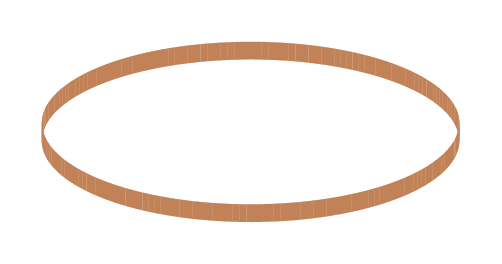
\begin{tikzpicture}[x=6.02321cm,y=6.02321cm]
\path[use as bounding box] (-0.469965,-0.219752) rectangle (0.469965,0.219752);
\path[fill=copper!82,draw=copper!82,line width=.08pt] (-0.008834,-0.189731) -- (0.005565,-0.189752) -- (0.005565,-0.152909) -- (-0.008834,-0.152888) -- cycle;
\path[fill=copper!82,draw=copper!82,line width=.08pt] (0.005565,-0.189752) -- (0.019957,-0.189589) -- (0.019957,-0.152747) -- (0.005565,-0.152909) -- cycle;
\path[fill=copper!82,draw=copper!82,line width=.08pt] (-0.023222,-0.189526) -- (-0.008834,-0.189731) -- (-0.008834,-0.152888) -- (-0.023222,-0.152684) -- cycle;
\path[fill=copper!82,draw=copper!82,line width=.08pt] (0.019957,-0.189589) -- (0.034328,-0.189243) -- (0.034328,-0.152401) -- (0.019957,-0.152747) -- cycle;
\path[fill=copper!82,draw=copper!82,line width=.08pt] (-0.037586,-0.189139) -- (-0.023222,-0.189526) -- (-0.023222,-0.152684) -- (-0.037586,-0.152297) -- cycle;
\path[fill=copper!82,draw=copper!82,line width=.08pt] (0.034328,-0.189243) -- (0.048662,-0.188714) -- (0.048662,-0.151872) -- (0.034328,-0.152401) -- cycle;
\path[fill=copper!82,draw=copper!82,line width=.08pt] (-0.051910,-0.188569) -- (-0.037586,-0.189139) -- (-0.037586,-0.152297) -- (-0.051910,-0.151726) -- cycle;
\path[fill=copper!82,draw=copper!82,line width=.08pt] (0.048662,-0.188714) -- (0.062944,-0.188003) -- (0.062944,-0.151161) -- (0.048662,-0.151872) -- cycle;
\path[fill=copper!82,draw=copper!82,line width=.08pt] (-0.066178,-0.187816) -- (-0.051910,-0.188569) -- (-0.051910,-0.151726) -- (-0.066178,-0.150974) -- cycle;
\path[fill=copper!82,draw=copper!82,line width=.08pt] (0.062944,-0.188003) -- (0.077159,-0.187110) -- (0.077159,-0.150268) -- (0.062944,-0.151161) -- cycle;
\path[fill=copper!82,draw=copper!82,line width=.08pt] (-0.080375,-0.186882) -- (-0.066178,-0.187816) -- (-0.066178,-0.150974) -- (-0.080375,-0.150040) -- cycle;
\path[fill=copper!82,draw=copper!82,line width=.08pt] (0.077159,-0.187110) -- (0.091291,-0.186037) -- (0.091291,-0.149194) -- (0.077159,-0.150268) -- cycle;
\path[fill=copper!82,draw=copper!82,line width=.08pt] (-0.094486,-0.185768) -- (-0.080375,-0.186882) -- (-0.080375,-0.150040) -- (-0.094486,-0.148926) -- cycle;
\path[fill=copper!82,draw=copper!82,line width=.08pt] (0.091291,-0.186037) -- (0.105325,-0.184784) -- (0.105325,-0.147941) -- (0.091291,-0.149194) -- cycle;
\path[fill=copper!82,draw=copper!82,line width=.08pt] (-0.108496,-0.184475) -- (-0.094486,-0.185768) -- (-0.094486,-0.148926) -- (-0.108496,-0.147632) -- cycle;
\path[fill=copper!82,draw=copper!82,line width=.08pt] (0.105325,-0.184784) -- (0.119246,-0.183353) -- (0.119246,-0.146510) -- (0.105325,-0.147941) -- cycle;
\path[fill=copper!82,draw=copper!82,line width=.08pt] (-0.122390,-0.183003) -- (-0.108496,-0.184475) -- (-0.108496,-0.147632) -- (-0.122390,-0.146161) -- cycle;
\path[fill=copper!82,draw=copper!82,line width=.08pt] (0.119246,-0.183353) -- (0.133040,-0.181745) -- (0.133040,-0.144903) -- (0.119246,-0.146510) -- cycle;
\path[fill=copper!82,draw=copper!82,line width=.08pt] (-0.136153,-0.181356) -- (-0.122390,-0.183003) -- (-0.122390,-0.146161) -- (-0.136153,-0.144513) -- cycle;
\path[fill=copper!82,draw=copper!82,line width=.08pt] (0.133040,-0.181745) -- (0.146691,-0.179963) -- (0.146691,-0.143120) -- (0.133040,-0.144903) -- cycle;
\path[fill=copper!82,draw=copper!82,line width=.08pt] (-0.149770,-0.179534) -- (-0.136153,-0.181356) -- (-0.136153,-0.144513) -- (-0.149770,-0.142691) -- cycle;
\path[fill=copper!82,draw=copper!82,line width=.08pt] (0.146691,-0.179963) -- (0.160186,-0.178007) -- (0.160186,-0.141165) -- (0.146691,-0.143120) -- cycle;
\path[fill=copper!82,draw=copper!82,line width=.08pt] (-0.163226,-0.177539) -- (-0.149770,-0.179534) -- (-0.149770,-0.142691) -- (-0.163226,-0.140697) -- cycle;
\path[fill=copper!82,draw=copper!82,line width=.08pt] (0.160186,-0.178007) -- (0.173508,-0.175881) -- (0.173508,-0.139038) -- (0.160186,-0.141165) -- cycle;
\path[fill=copper!82,draw=copper!82,line width=.08pt] (-0.176508,-0.175374) -- (-0.163226,-0.177539) -- (-0.163226,-0.140697) -- (-0.176508,-0.138532) -- cycle;
\path[fill=copper!82,draw=copper!82,line width=.08pt] (0.173508,-0.175881) -- (0.186645,-0.173586) -- (0.186645,-0.136743) -- (0.173508,-0.139038) -- cycle;
\path[fill=copper!82,draw=copper!82,line width=.08pt] (-0.189601,-0.173041) -- (-0.176508,-0.175374) -- (-0.176508,-0.138532) -- (-0.189601,-0.136199) -- cycle;
\path[fill=copper!82,draw=copper!82,line width=.08pt] (0.186645,-0.173586) -- (0.199582,-0.171124) -- (0.199582,-0.134282) -- (0.186645,-0.136743) -- cycle;
\path[fill=copper!82,draw=copper!82,line width=.08pt] (-0.202490,-0.170543) -- (-0.189601,-0.173041) -- (-0.189601,-0.136199) -- (-0.202490,-0.133700) -- cycle;
\path[fill=copper!82,draw=copper!82,line width=.08pt] (0.199582,-0.171124) -- (0.212306,-0.168500) -- (0.212306,-0.131657) -- (0.199582,-0.134282) -- cycle;
\path[fill=copper!82,draw=copper!82,line width=.08pt] (-0.215163,-0.167881) -- (-0.202490,-0.170543) -- (-0.202490,-0.133700) -- (-0.215163,-0.131039) -- cycle;
\path[fill=copper!82,draw=copper!82,line width=.08pt] (0.212306,-0.168500) -- (0.224802,-0.165714) -- (0.224802,-0.128872) -- (0.212306,-0.131657) -- cycle;
\path[fill=copper!82,draw=copper!82,line width=.08pt] (-0.227606,-0.165060) -- (-0.215163,-0.167881) -- (-0.215163,-0.131039) -- (-0.227606,-0.128217) -- cycle;
\path[fill=copper!82,draw=copper!82,line width=.08pt] (0.224802,-0.165714) -- (0.237057,-0.162771) -- (0.237057,-0.125929) -- (0.224802,-0.128872) -- cycle;
\path[fill=copper!82,draw=copper!82,line width=.08pt] (-0.239804,-0.162081) -- (-0.227606,-0.165060) -- (-0.227606,-0.128217) -- (-0.239804,-0.125239) -- cycle;
\path[fill=copper!82,draw=copper!82,line width=.08pt] (0.237057,-0.162771) -- (0.249058,-0.159673) -- (0.249058,-0.122831) -- (0.237057,-0.125929) -- cycle;
\path[fill=copper!82,draw=copper!82,line width=.08pt] (-0.251746,-0.158949) -- (-0.239804,-0.162081) -- (-0.239804,-0.125239) -- (-0.251746,-0.122106) -- cycle;
\path[fill=copper!82,draw=copper!82,line width=.08pt] (0.249058,-0.159673) -- (0.260793,-0.156424) -- (0.260793,-0.119582) -- (0.249058,-0.122831) -- cycle;
\path[fill=copper!82,draw=copper!82,line width=.08pt] (-0.263419,-0.155666) -- (-0.251746,-0.158949) -- (-0.251746,-0.122106) -- (-0.263419,-0.118823) -- cycle;
\path[fill=copper!82,draw=copper!82,line width=.08pt] (0.260793,-0.156424) -- (0.272248,-0.153028) -- (0.272248,-0.116185) -- (0.260793,-0.119582) -- cycle;
\path[fill=copper!82,draw=copper!82,line width=.08pt] (-0.274809,-0.152236) -- (-0.263419,-0.155666) -- (-0.263419,-0.118823) -- (-0.274809,-0.115394) -- cycle;
\path[fill=copper!82,draw=copper!82,line width=.08pt] (0.272248,-0.153028) -- (0.283412,-0.149487) -- (0.283412,-0.112644) -- (0.272248,-0.116185) -- cycle;
\path[fill=copper!82,draw=copper!82,line width=.08pt] (-0.285905,-0.148663) -- (-0.274809,-0.152236) -- (-0.274809,-0.115394) -- (-0.285905,-0.111821) -- cycle;
\path[fill=copper!82,draw=copper!82,line width=.08pt] (0.283412,-0.149487) -- (0.294273,-0.145805) -- (0.294273,-0.108963) -- (0.283412,-0.112644) -- cycle;
\path[fill=copper!82,draw=copper!82,line width=.08pt] (-0.296695,-0.144950) -- (-0.285905,-0.148663) -- (-0.285905,-0.111821) -- (-0.296695,-0.108108) -- cycle;
\path[fill=copper!82,draw=copper!82,line width=.08pt] (0.294273,-0.145805) -- (0.304818,-0.141988) -- (0.304818,-0.105145) -- (0.294273,-0.108963) -- cycle;
\path[fill=copper!82,draw=copper!82,line width=.08pt] (-0.307167,-0.141102) -- (-0.296695,-0.144950) -- (-0.296695,-0.108108) -- (-0.307167,-0.104260) -- cycle;
\path[fill=copper!82,draw=copper!82,line width=.08pt] (0.304818,-0.141988) -- (0.315037,-0.138038) -- (0.315037,-0.101195) -- (0.304818,-0.105145) -- cycle;
\path[fill=copper!82,draw=copper!82,line width=.08pt] (-0.317311,-0.137123) -- (-0.307167,-0.141102) -- (-0.307167,-0.104260) -- (-0.317311,-0.100281) -- cycle;
\path[fill=copper!82,draw=copper!82,line width=.08pt] (0.315037,-0.138038) -- (0.324918,-0.133960) -- (0.324918,-0.097117) -- (0.315037,-0.101195) -- cycle;
\path[fill=copper!82,draw=copper!82,line width=.08pt] (-0.327114,-0.133016) -- (-0.317311,-0.137123) -- (-0.317311,-0.100281) -- (-0.327114,-0.096174) -- cycle;
\path[fill=copper!82,draw=copper!82,line width=.08pt] (0.324918,-0.133960) -- (0.334452,-0.129758) -- (0.334452,-0.092916) -- (0.324918,-0.097117) -- cycle;
\path[fill=copper!82,draw=copper!82,line width=.08pt] (-0.336567,-0.128787) -- (-0.327114,-0.133016) -- (-0.327114,-0.096174) -- (-0.336567,-0.091945) -- cycle;
\path[fill=copper!82,draw=copper!82,line width=.08pt] (0.334452,-0.129758) -- (0.343628,-0.125437) -- (0.343628,-0.088595) -- (0.334452,-0.092916) -- cycle;
\path[fill=copper!82,draw=copper!82,line width=.08pt] (-0.345660,-0.124440) -- (-0.336567,-0.128787) -- (-0.336567,-0.091945) -- (-0.345660,-0.087597) -- cycle;
\path[fill=copper!82,draw=copper!82,line width=.08pt] (0.343628,-0.125437) -- (0.352435,-0.121001) -- (0.352435,-0.084159) -- (0.343628,-0.088595) -- cycle;
\path[fill=copper!82,draw=copper!82,line width=.08pt] (-0.354383,-0.119979) -- (-0.345660,-0.124440) -- (-0.345660,-0.087597) -- (-0.354383,-0.083136) -- cycle;
\path[fill=copper!82,draw=copper!82,line width=.08pt] (0.352435,-0.121001) -- (0.360865,-0.116456) -- (0.360865,-0.079613) -- (0.352435,-0.084159) -- cycle;
\path[fill=copper!82,draw=copper!82,line width=.08pt] (-0.362726,-0.115409) -- (-0.354383,-0.119979) -- (-0.354383,-0.083136) -- (-0.362726,-0.078567) -- cycle;
\path[fill=copper!82,draw=copper!82,line width=.08pt] (0.360865,-0.116456) -- (0.368909,-0.111805) -- (0.368909,-0.074963) -- (0.360865,-0.079613) -- cycle;
\path[fill=copper!82,draw=copper!82,line width=.08pt] (-0.370681,-0.110735) -- (-0.362726,-0.115409) -- (-0.362726,-0.078567) -- (-0.370681,-0.073893) -- cycle;
\path[fill=copper!82,draw=copper!82,line width=.08pt] (0.368909,-0.111805) -- (0.376558,-0.107055) -- (0.376558,-0.070213) -- (0.368909,-0.074963) -- cycle;
\path[fill=copper!82,draw=copper!82,line width=.08pt] (-0.378238,-0.105963) -- (-0.370681,-0.110735) -- (-0.370681,-0.073893) -- (-0.378238,-0.069121) -- cycle;
\path[fill=copper!82,draw=copper!82,line width=.08pt] (0.376558,-0.107055) -- (0.383803,-0.102210) -- (0.383803,-0.065367) -- (0.376558,-0.070213) -- cycle;
\path[fill=copper!82,draw=copper!82,line width=.08pt] (-0.385391,-0.101097) -- (-0.378238,-0.105963) -- (-0.378238,-0.069121) -- (-0.385391,-0.064254) -- cycle;
\path[fill=copper!82,draw=copper!82,line width=.08pt] (0.383803,-0.102210) -- (0.390638,-0.097275) -- (0.390638,-0.060432) -- (0.383803,-0.065367) -- cycle;
\path[fill=copper!82,draw=copper!82,line width=.08pt] (-0.392131,-0.096142) -- (-0.385391,-0.101097) -- (-0.385391,-0.064254) -- (-0.392131,-0.059300) -- cycle;
\path[fill=copper!82,draw=copper!82,line width=.08pt] (0.390638,-0.097275) -- (0.397054,-0.092255) -- (0.397054,-0.055413) -- (0.390638,-0.060432) -- cycle;
\path[fill=copper!82,draw=copper!82,line width=.08pt] (-0.398451,-0.091104) -- (-0.392131,-0.096142) -- (-0.392131,-0.059300) -- (-0.398451,-0.054262) -- cycle;
\path[fill=copper!82,draw=copper!82,line width=.08pt] (0.397054,-0.092255) -- (0.403045,-0.087157) -- (0.403045,-0.050314) -- (0.397054,-0.055413) -- cycle;
\path[fill=copper!82,draw=copper!82,line width=.08pt] (-0.404345,-0.085989) -- (-0.398451,-0.091104) -- (-0.398451,-0.054262) -- (-0.404345,-0.049146) -- cycle;
\path[fill=copper!82,draw=copper!82,line width=.08pt] (0.403045,-0.087157) -- (0.408604,-0.081984) -- (0.408604,-0.045142) -- (0.403045,-0.050314) -- cycle;
\path[fill=copper!82,draw=copper!82,line width=.08pt] (-0.409806,-0.080800) -- (-0.404345,-0.085989) -- (-0.404345,-0.049146) -- (-0.409806,-0.043958) -- cycle;
\path[fill=copper!82,draw=copper!82,line width=.08pt] (0.408604,-0.081984) -- (0.413726,-0.076744) -- (0.413726,-0.039902) -- (0.408604,-0.045142) -- cycle;
\path[fill=copper!82,draw=copper!82,line width=.08pt] (-0.414827,-0.075546) -- (-0.409806,-0.080800) -- (-0.409806,-0.043958) -- (-0.414827,-0.038703) -- cycle;
\path[fill=copper!82,draw=copper!82,line width=.08pt] (0.413726,-0.076744) -- (0.418405,-0.071442) -- (0.418405,-0.034599) -- (0.413726,-0.039902) -- cycle;
\path[fill=copper!82,draw=copper!82,line width=.08pt] (-0.419405,-0.070229) -- (-0.414827,-0.075546) -- (-0.414827,-0.038703) -- (-0.419405,-0.033387) -- cycle;
\path[fill=copper!82,draw=copper!82,line width=.08pt] (0.418405,-0.071442) -- (0.422635,-0.066082) -- (0.422635,-0.029240) -- (0.418405,-0.034599) -- cycle;
\path[fill=copper!82,draw=copper!82,line width=.08pt] (-0.423533,-0.064858) -- (-0.419405,-0.070229) -- (-0.419405,-0.033387) -- (-0.423533,-0.028016) -- cycle;
\path[fill=copper!82,draw=copper!82,line width=.08pt] (0.422635,-0.066082) -- (0.426414,-0.060672) -- (0.426414,-0.023829) -- (0.422635,-0.029240) -- cycle;
\path[fill=copper!82,draw=copper!82,line width=.08pt] (-0.427208,-0.059437) -- (-0.423533,-0.064858) -- (-0.423533,-0.028016) -- (-0.427208,-0.022594) -- cycle;
\path[fill=copper!82,draw=copper!82,line width=.08pt] (0.426414,-0.060672) -- (0.429735,-0.055216) -- (0.429735,-0.018373) -- (0.426414,-0.023829) -- cycle;
\path[fill=copper!82,draw=copper!82,line width=.08pt] (-0.430425,-0.053971) -- (-0.427208,-0.059437) -- (-0.427208,-0.022594) -- (-0.430425,-0.017129) -- cycle;
\path[fill=copper!82,draw=copper!82,line width=.08pt] (0.429735,-0.055216) -- (0.432597,-0.049721) -- (0.432597,-0.012878) -- (0.429735,-0.018373) -- cycle;
\path[fill=copper!82,draw=copper!82,line width=.08pt] (-0.433182,-0.048468) -- (-0.430425,-0.053971) -- (-0.430425,-0.017129) -- (-0.433182,-0.011626) -- cycle;
\path[fill=copper!82,draw=copper!82,line width=.08pt] (0.432597,-0.049721) -- (0.434995,-0.044192) -- (0.434995,-0.007350) -- (0.432597,-0.012878) -- cycle;
\path[fill=copper!82,draw=copper!82,line width=.08pt] (-0.435475,-0.042933) -- (-0.433182,-0.048468) -- (-0.433182,-0.011626) -- (-0.435475,-0.006090) -- cycle;
\path[fill=copper!82,draw=copper!82,line width=.08pt] (0.434995,-0.044192) -- (0.436927,-0.038636) -- (0.436927,-0.001793) -- (0.434995,-0.007350) -- cycle;
\path[fill=copper!82,draw=copper!82,line width=.08pt] (-0.437301,-0.037371) -- (-0.435475,-0.042933) -- (-0.435475,-0.006090) -- (-0.437301,-0.000529) -- cycle;
\path[fill=copper!82,draw=copper!82,line width=.08pt] (0.436927,-0.038636) -- (0.438392,-0.033058) -- (0.438392,0.003784) -- (0.436927,-0.001793) -- cycle;
\path[fill=copper!82,draw=copper!82,line width=.08pt] (-0.438659,-0.031789) -- (-0.437301,-0.037371) -- (-0.437301,-0.000529) -- (-0.438659,0.005053) -- cycle;
\path[fill=copper!82,draw=copper!82,line width=.08pt] (0.438392,-0.033058) -- (0.439387,-0.027464) -- (0.439387,0.009378) -- (0.438392,0.003784) -- cycle;
\path[fill=copper!82,draw=copper!82,line width=.08pt] (-0.439547,-0.026193) -- (-0.438659,-0.031789) -- (-0.438659,0.005053) -- (-0.439547,0.010650) -- cycle;
\path[fill=copper!82,draw=copper!82,line width=.08pt] (0.439387,-0.027464) -- (0.439911,-0.021861) -- (0.439911,0.014981) -- (0.439387,0.009378) -- cycle;
\path[fill=copper!82,draw=copper!82,line width=.08pt] (-0.439965,-0.020588) -- (-0.439547,-0.026193) -- (-0.439547,0.010650) -- (-0.439965,0.016254) -- cycle;
\path[fill=copper!82,draw=copper!82,line width=.08pt] (0.439911,-0.021861) -- (0.439965,-0.016254) -- (0.439965,0.020588) -- (0.439911,0.014981) -- cycle;
\path[fill=copper!82,draw=copper!82,line width=.08pt] (-0.439911,-0.014981) -- (-0.439965,-0.020588) -- (-0.439965,0.016254) -- (-0.439911,0.021861) -- cycle;
\path[fill=copper!82,draw=copper!82,line width=.08pt] (0.439965,-0.016254) -- (0.439547,-0.010650) -- (0.439547,0.026193) -- (0.439965,0.020588) -- cycle;
\path[fill=copper!82,draw=copper!82,line width=.08pt] (-0.439387,-0.009378) -- (-0.439911,-0.014981) -- (-0.439911,0.021861) -- (-0.439387,0.027464) -- cycle;
\path[fill=copper!82,draw=copper!82,line width=.08pt] (0.439547,-0.010650) -- (0.438659,-0.005053) -- (0.438659,0.031789) -- (0.439547,0.026193) -- cycle;
\path[fill=copper!82,draw=copper!82,line width=.08pt] (-0.438392,-0.003784) -- (-0.439387,-0.009378) -- (-0.439387,0.027464) -- (-0.438392,0.033058) -- cycle;
\path[fill=copper!82,draw=copper!82,line width=.08pt] (0.438659,-0.005053) -- (0.437301,0.000529) -- (0.437301,0.037371) -- (0.438659,0.031789) -- cycle;
\path[fill=copper!82,draw=copper!82,line width=.08pt] (-0.436927,0.001793) -- (-0.438392,-0.003784) -- (-0.438392,0.033058) -- (-0.436927,0.038636) -- cycle;
\path[fill=copper!82,draw=copper!82,line width=.08pt] (0.437301,0.000529) -- (0.435475,0.006090) -- (0.435475,0.042933) -- (0.437301,0.037371) -- cycle;
\path[fill=copper!82,draw=copper!82,line width=.08pt] (-0.434995,0.007350) -- (-0.436927,0.001793) -- (-0.436927,0.038636) -- (-0.434995,0.044192) -- cycle;
\path[fill=copper!82,draw=copper!82,line width=.08pt] (0.435475,0.006090) -- (0.433182,0.011626) -- (0.433182,0.048468) -- (0.435475,0.042933) -- cycle;
\path[fill=copper!82,draw=copper!82,line width=.08pt] (-0.432597,0.012878) -- (-0.434995,0.007350) -- (-0.434995,0.044192) -- (-0.432597,0.049721) -- cycle;
\path[fill=copper!82,draw=copper!82,line width=.08pt] (0.433182,0.011626) -- (0.430425,0.017129) -- (0.430425,0.053971) -- (0.433182,0.048468) -- cycle;
\path[fill=copper!82,draw=copper!82,line width=.08pt] (-0.429735,0.018373) -- (-0.432597,0.012878) -- (-0.432597,0.049721) -- (-0.429735,0.055216) -- cycle;
\path[fill=copper!82,draw=copper!82,line width=.08pt] (0.430425,0.017129) -- (0.427208,0.022594) -- (0.427208,0.059437) -- (0.430425,0.053971) -- cycle;
\path[fill=copper!82,draw=copper!82,line width=.08pt] (-0.426414,0.023829) -- (-0.429735,0.018373) -- (-0.429735,0.055216) -- (-0.426414,0.060672) -- cycle;
\path[fill=copper!82,draw=copper!82,line width=.08pt] (0.427208,0.022594) -- (0.423533,0.028016) -- (0.423533,0.064858) -- (0.427208,0.059437) -- cycle;
\path[fill=copper!82,draw=copper!82,line width=.08pt] (-0.422635,0.029240) -- (-0.426414,0.023829) -- (-0.426414,0.060672) -- (-0.422635,0.066082) -- cycle;
\path[fill=copper!82,draw=copper!82,line width=.08pt] (0.423533,0.028016) -- (0.419405,0.033387) -- (0.419405,0.070229) -- (0.423533,0.064858) -- cycle;
\path[fill=copper!82,draw=copper!82,line width=.08pt] (-0.418405,0.034599) -- (-0.422635,0.029240) -- (-0.422635,0.066082) -- (-0.418405,0.071442) -- cycle;
\path[fill=copper!82,draw=copper!82,line width=.08pt] (0.419405,0.033387) -- (0.414827,0.038703) -- (0.414827,0.075546) -- (0.419405,0.070229) -- cycle;
\path[fill=copper!82,draw=copper!82,line width=.08pt] (-0.413726,0.039902) -- (-0.418405,0.034599) -- (-0.418405,0.071442) -- (-0.413726,0.076744) -- cycle;
\path[fill=copper!82,draw=copper!82,line width=.08pt] (0.414827,0.038703) -- (0.409806,0.043958) -- (0.409806,0.080800) -- (0.414827,0.075546) -- cycle;
\path[fill=copper!82,draw=copper!82,line width=.08pt] (-0.408604,0.045142) -- (-0.413726,0.039902) -- (-0.413726,0.076744) -- (-0.408604,0.081984) -- cycle;
\path[fill=copper!82,draw=copper!82,line width=.08pt] (0.409806,0.043958) -- (0.404345,0.049146) -- (0.404345,0.085989) -- (0.409806,0.080800) -- cycle;
\path[fill=copper!82,draw=copper!82,line width=.08pt] (-0.403045,0.050314) -- (-0.408604,0.045142) -- (-0.408604,0.081984) -- (-0.403045,0.087157) -- cycle;
\path[fill=copper!82,draw=copper!82,line width=.08pt] (0.404345,0.049146) -- (0.398451,0.054262) -- (0.398451,0.091104) -- (0.404345,0.085989) -- cycle;
\path[fill=copper!82,draw=copper!82,line width=.08pt] (-0.397054,0.055413) -- (-0.403045,0.050314) -- (-0.403045,0.087157) -- (-0.397054,0.092255) -- cycle;
\path[fill=copper!82,draw=copper!82,line width=.08pt] (0.398451,0.054262) -- (0.392131,0.059300) -- (0.392131,0.096142) -- (0.398451,0.091104) -- cycle;
\path[fill=copper!82,draw=copper!82,line width=.08pt] (-0.390638,0.060432) -- (-0.397054,0.055413) -- (-0.397054,0.092255) -- (-0.390638,0.097275) -- cycle;
\path[fill=copper!82,draw=copper!82,line width=.08pt] (0.392131,0.059300) -- (0.385391,0.064254) -- (0.385391,0.101097) -- (0.392131,0.096142) -- cycle;
\path[fill=copper!82,draw=copper!82,line width=.08pt] (-0.383803,0.065367) -- (-0.390638,0.060432) -- (-0.390638,0.097275) -- (-0.383803,0.102210) -- cycle;
\path[fill=copper!82,draw=copper!82,line width=.08pt] (0.385391,0.064254) -- (0.378238,0.069121) -- (0.378238,0.105963) -- (0.385391,0.101097) -- cycle;
\path[fill=copper!82,draw=copper!82,line width=.08pt] (-0.376558,0.070213) -- (-0.383803,0.065367) -- (-0.383803,0.102210) -- (-0.376558,0.107055) -- cycle;
\path[fill=copper!82,draw=copper!82,line width=.08pt] (0.378238,0.069121) -- (0.370681,0.073893) -- (0.370681,0.110735) -- (0.378238,0.105963) -- cycle;
\path[fill=copper!82,draw=copper!82,line width=.08pt] (-0.368909,0.074963) -- (-0.376558,0.070213) -- (-0.376558,0.107055) -- (-0.368909,0.111805) -- cycle;
\path[fill=copper!82,draw=copper!82,line width=.08pt] (0.370681,0.073893) -- (0.362726,0.078567) -- (0.362726,0.115409) -- (0.370681,0.110735) -- cycle;
\path[fill=copper!82,draw=copper!82,line width=.08pt] (-0.360865,0.079613) -- (-0.368909,0.074963) -- (-0.368909,0.111805) -- (-0.360865,0.116456) -- cycle;
\path[fill=copper!82,draw=copper!82,line width=.08pt] (0.362726,0.078567) -- (0.354383,0.083136) -- (0.354383,0.119979) -- (0.362726,0.115409) -- cycle;
\path[fill=copper!82,draw=copper!82,line width=.08pt] (-0.352435,0.084159) -- (-0.360865,0.079613) -- (-0.360865,0.116456) -- (-0.352435,0.121001) -- cycle;
\path[fill=copper!82,draw=copper!82,line width=.08pt] (0.354383,0.083136) -- (0.345660,0.087597) -- (0.345660,0.124440) -- (0.354383,0.119979) -- cycle;
\path[fill=copper!82,draw=copper!82,line width=.08pt] (-0.343628,0.088595) -- (-0.352435,0.084159) -- (-0.352435,0.121001) -- (-0.343628,0.125437) -- cycle;
\path[fill=copper!82,draw=copper!82,line width=.08pt] (0.345660,0.087597) -- (0.336567,0.091945) -- (0.336567,0.128787) -- (0.345660,0.124440) -- cycle;
\path[fill=copper!82,draw=copper!82,line width=.08pt] (-0.334452,0.092916) -- (-0.343628,0.088595) -- (-0.343628,0.125437) -- (-0.334452,0.129758) -- cycle;
\path[fill=copper!82,draw=copper!82,line width=.08pt] (0.336567,0.091945) -- (0.327114,0.096174) -- (0.327114,0.133016) -- (0.336567,0.128787) -- cycle;
\path[fill=copper!82,draw=copper!82,line width=.08pt] (-0.324918,0.097117) -- (-0.334452,0.092916) -- (-0.334452,0.129758) -- (-0.324918,0.133960) -- cycle;
\path[fill=copper!82,draw=copper!82,line width=.08pt] (0.327114,0.096174) -- (0.317311,0.100281) -- (0.317311,0.137123) -- (0.327114,0.133016) -- cycle;
\path[fill=copper!82,draw=copper!82,line width=.08pt] (-0.315037,0.101195) -- (-0.324918,0.097117) -- (-0.324918,0.133960) -- (-0.315037,0.138038) -- cycle;
\path[fill=copper!82,draw=copper!82,line width=.08pt] (0.317311,0.100281) -- (0.307167,0.104260) -- (0.307167,0.141102) -- (0.317311,0.137123) -- cycle;
\path[fill=copper!82,draw=copper!82,line width=.08pt] (-0.304818,0.105145) -- (-0.315037,0.101195) -- (-0.315037,0.138038) -- (-0.304818,0.141988) -- cycle;
\path[fill=copper!82,draw=copper!82,line width=.08pt] (0.307167,0.104260) -- (0.296695,0.108108) -- (0.296695,0.144950) -- (0.307167,0.141102) -- cycle;
\path[fill=copper!82,draw=copper!82,line width=.08pt] (-0.294273,0.108963) -- (-0.304818,0.105145) -- (-0.304818,0.141988) -- (-0.294273,0.145805) -- cycle;
\path[fill=copper!82,draw=copper!82,line width=.08pt] (0.296695,0.108108) -- (0.285905,0.111821) -- (0.285905,0.148663) -- (0.296695,0.144950) -- cycle;
\path[fill=copper!82,draw=copper!82,line width=.08pt] (-0.283412,0.112644) -- (-0.294273,0.108963) -- (-0.294273,0.145805) -- (-0.283412,0.149487) -- cycle;
\path[fill=copper!82,draw=copper!82,line width=.08pt] (0.285905,0.111821) -- (0.274809,0.115394) -- (0.274809,0.152236) -- (0.285905,0.148663) -- cycle;
\path[fill=copper!82,draw=copper!82,line width=.08pt] (-0.272248,0.116185) -- (-0.283412,0.112644) -- (-0.283412,0.149487) -- (-0.272248,0.153028) -- cycle;
\path[fill=copper!82,draw=copper!82,line width=.08pt] (0.274809,0.115394) -- (0.263419,0.118823) -- (0.263419,0.155666) -- (0.274809,0.152236) -- cycle;
\path[fill=copper!82,draw=copper!82,line width=.08pt] (-0.260793,0.119582) -- (-0.272248,0.116185) -- (-0.272248,0.153028) -- (-0.260793,0.156424) -- cycle;
\path[fill=copper!82,draw=copper!82,line width=.08pt] (0.263419,0.118823) -- (0.251746,0.122106) -- (0.251746,0.158949) -- (0.263419,0.155666) -- cycle;
\path[fill=copper!82,draw=copper!82,line width=.08pt] (-0.249058,0.122831) -- (-0.260793,0.119582) -- (-0.260793,0.156424) -- (-0.249058,0.159673) -- cycle;
\path[fill=copper!82,draw=copper!82,line width=.08pt] (0.251746,0.122106) -- (0.239804,0.125239) -- (0.239804,0.162081) -- (0.251746,0.158949) -- cycle;
\path[fill=copper!82,draw=copper!82,line width=.08pt] (-0.237057,0.125929) -- (-0.249058,0.122831) -- (-0.249058,0.159673) -- (-0.237057,0.162771) -- cycle;
\path[fill=copper!82,draw=copper!82,line width=.08pt] (0.239804,0.125239) -- (0.227606,0.128217) -- (0.227606,0.165060) -- (0.239804,0.162081) -- cycle;
\path[fill=copper!82,draw=copper!82,line width=.08pt] (-0.224802,0.128872) -- (-0.237057,0.125929) -- (-0.237057,0.162771) -- (-0.224802,0.165714) -- cycle;
\path[fill=copper!82,draw=copper!82,line width=.08pt] (0.227606,0.128217) -- (0.215163,0.131039) -- (0.215163,0.167881) -- (0.227606,0.165060) -- cycle;
\path[fill=copper!82,draw=copper!82,line width=.08pt] (-0.212306,0.131657) -- (-0.224802,0.128872) -- (-0.224802,0.165714) -- (-0.212306,0.168500) -- cycle;
\path[fill=copper!82,draw=copper!82,line width=.08pt] (0.215163,0.131039) -- (0.202490,0.133700) -- (0.202490,0.170543) -- (0.215163,0.167881) -- cycle;
\path[fill=copper!82,draw=copper!82,line width=.08pt] (-0.199582,0.134282) -- (-0.212306,0.131657) -- (-0.212306,0.168500) -- (-0.199582,0.171124) -- cycle;
\path[fill=copper!82,draw=copper!82,line width=.08pt] (0.202490,0.133700) -- (0.189601,0.136199) -- (0.189601,0.173041) -- (0.202490,0.170543) -- cycle;
\path[fill=copper!82,draw=copper!82,line width=.08pt] (-0.186645,0.136743) -- (-0.199582,0.134282) -- (-0.199582,0.171124) -- (-0.186645,0.173586) -- cycle;
\path[fill=copper!82,draw=copper!82,line width=.08pt] (0.189601,0.136199) -- (0.176508,0.138532) -- (0.176508,0.175374) -- (0.189601,0.173041) -- cycle;
\path[fill=copper!82,draw=copper!82,line width=.08pt] (-0.173508,0.139038) -- (-0.186645,0.136743) -- (-0.186645,0.173586) -- (-0.173508,0.175881) -- cycle;
\path[fill=copper!82,draw=copper!82,line width=.08pt] (0.176508,0.138532) -- (0.163226,0.140697) -- (0.163226,0.177539) -- (0.176508,0.175374) -- cycle;
\path[fill=copper!82,draw=copper!82,line width=.08pt] (-0.160186,0.141165) -- (-0.173508,0.139038) -- (-0.173508,0.175881) -- (-0.160186,0.178007) -- cycle;
\path[fill=copper!82,draw=copper!82,line width=.08pt] (0.163226,0.140697) -- (0.149770,0.142691) -- (0.149770,0.179534) -- (0.163226,0.177539) -- cycle;
\path[fill=copper!82,draw=copper!82,line width=.08pt] (-0.146691,0.143120) -- (-0.160186,0.141165) -- (-0.160186,0.178007) -- (-0.146691,0.179963) -- cycle;
\path[fill=copper!82,draw=copper!82,line width=.08pt] (0.149770,0.142691) -- (0.136153,0.144513) -- (0.136153,0.181356) -- (0.149770,0.179534) -- cycle;
\path[fill=copper!82,draw=copper!82,line width=.08pt] (-0.133040,0.144903) -- (-0.146691,0.143120) -- (-0.146691,0.179963) -- (-0.133040,0.181745) -- cycle;
\path[fill=copper!82,draw=copper!82,line width=.08pt] (0.136153,0.144513) -- (0.122390,0.146161) -- (0.122390,0.183003) -- (0.136153,0.181356) -- cycle;
\path[fill=copper!82,draw=copper!82,line width=.08pt] (-0.119246,0.146510) -- (-0.133040,0.144903) -- (-0.133040,0.181745) -- (-0.119246,0.183353) -- cycle;
\path[fill=copper!82,draw=copper!82,line width=.08pt] (0.122390,0.146161) -- (0.108496,0.147632) -- (0.108496,0.184475) -- (0.122390,0.183003) -- cycle;
\path[fill=copper!82,draw=copper!82,line width=.08pt] (-0.105325,0.147941) -- (-0.119246,0.146510) -- (-0.119246,0.183353) -- (-0.105325,0.184784) -- cycle;
\path[fill=copper!82,draw=copper!82,line width=.08pt] (0.108496,0.147632) -- (0.094486,0.148926) -- (0.094486,0.185768) -- (0.108496,0.184475) -- cycle;
\path[fill=copper!82,draw=copper!82,line width=.08pt] (-0.091291,0.149194) -- (-0.105325,0.147941) -- (-0.105325,0.184784) -- (-0.091291,0.186037) -- cycle;
\path[fill=copper!82,draw=copper!82,line width=.08pt] (0.094486,0.148926) -- (0.080375,0.150040) -- (0.080375,0.186882) -- (0.094486,0.185768) -- cycle;
\path[fill=copper!82,draw=copper!82,line width=.08pt] (-0.077159,0.150268) -- (-0.091291,0.149194) -- (-0.091291,0.186037) -- (-0.077159,0.187110) -- cycle;
\path[fill=copper!82,draw=copper!82,line width=.08pt] (0.080375,0.150040) -- (0.066178,0.150974) -- (0.066178,0.187816) -- (0.080375,0.186882) -- cycle;
\path[fill=copper!82,draw=copper!82,line width=.08pt] (-0.062944,0.151161) -- (-0.077159,0.150268) -- (-0.077159,0.187110) -- (-0.062944,0.188003) -- cycle;
\path[fill=copper!82,draw=copper!82,line width=.08pt] (0.066178,0.150974) -- (0.051910,0.151726) -- (0.051910,0.188569) -- (0.066178,0.187816) -- cycle;
\path[fill=copper!82,draw=copper!82,line width=.08pt] (-0.048662,0.151872) -- (-0.062944,0.151161) -- (-0.062944,0.188003) -- (-0.048662,0.188714) -- cycle;
\path[fill=copper!82,draw=copper!82,line width=.08pt] (0.051910,0.151726) -- (0.037586,0.152297) -- (0.037586,0.189139) -- (0.051910,0.188569) -- cycle;
\path[fill=copper!82,draw=copper!82,line width=.08pt] (-0.034328,0.152401) -- (-0.048662,0.151872) -- (-0.048662,0.188714) -- (-0.034328,0.189243) -- cycle;
\path[fill=copper!82,draw=copper!82,line width=.08pt] (0.037586,0.152297) -- (0.023222,0.152684) -- (0.023222,0.189526) -- (0.037586,0.189139) -- cycle;
\path[fill=copper!82,draw=copper!82,line width=.08pt] (-0.019957,0.152747) -- (-0.034328,0.152401) -- (-0.034328,0.189243) -- (-0.019957,0.189589) -- cycle;
\path[fill=copper!82,draw=copper!82,line width=.08pt] (0.023222,0.152684) -- (0.008834,0.152888) -- (0.008834,0.189731) -- (0.023222,0.189526) -- cycle;
\path[fill=copper!82,draw=copper!82,line width=.08pt] (-0.005565,0.152909) -- (-0.019957,0.152747) -- (-0.019957,0.189589) -- (-0.005565,0.189752) -- cycle;
\path[fill=copper!82,draw=copper!82,line width=.08pt] (0.008834,0.152888) -- (-0.005565,0.152909) -- (-0.005565,0.189752) -- (0.008834,0.189731) -- cycle;
\end{tikzpicture}
}

\newcommand{\AntennaFigureE}{%
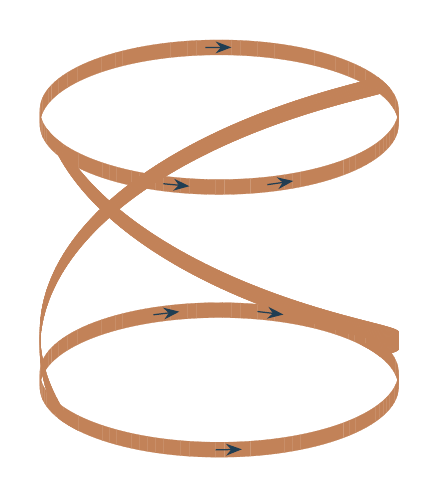
\begin{tikzpicture}[x=5.17475cm,y=5.17475cm]
\path[use as bounding box] (-0.470000,-0.542102) rectangle (0.470000,0.542102);
\path[fill=copper!82,draw=copper!82,line width=.08pt] (-0.008834,0.132641) -- (0.012763,0.132678) -- (0.012763,0.169521) -- (-0.008834,0.169483) -- cycle;
\path[fill=copper!82,draw=copper!82,line width=.08pt] (-0.030408,0.133016) -- (-0.008834,0.132641) -- (-0.008834,0.169483) -- (-0.030408,0.169858) -- cycle;
\path[fill=copper!82,draw=copper!82,line width=.08pt] (0.012763,0.132678) -- (0.034328,0.133128) -- (0.034328,0.169971) -- (0.012763,0.169521) -- cycle;
\path[fill=copper!82,draw=copper!82,line width=.08pt] (-0.051910,0.133803) -- (-0.030408,0.133016) -- (-0.030408,0.169858) -- (-0.051910,0.170645) -- cycle;
\path[fill=copper!82,draw=copper!82,line width=.08pt] (0.034328,0.133128) -- (0.055810,0.133990) -- (0.055810,0.170832) -- (0.034328,0.169971) -- cycle;
\path[fill=copper!82,draw=copper!82,line width=.08pt] (-0.073286,0.135000) -- (-0.051910,0.133803) -- (-0.051910,0.170645) -- (-0.073286,0.171842) -- cycle;
\path[fill=copper!82,draw=copper!82,line width=.08pt] (0.055810,0.133990) -- (0.077159,0.135261) -- (0.077159,0.172104) -- (0.055810,0.170832) -- cycle;
\path[fill=copper!82,draw=copper!82,line width=.08pt] (-0.094486,0.136603) -- (-0.073286,0.135000) -- (-0.073286,0.171842) -- (-0.094486,0.173446) -- cycle;
\path[fill=copper!82,draw=copper!82,line width=.08pt] (0.077159,0.135261) -- (0.098321,0.136939) -- (0.098321,0.173781) -- (0.077159,0.172104) -- cycle;
\path[fill=copper!82,draw=copper!82,line width=.08pt] (-0.115459,0.138610) -- (-0.094486,0.136603) -- (-0.094486,0.173446) -- (-0.115459,0.175453) -- cycle;
\path[fill=copper!82,draw=copper!82,line width=.08pt] (0.098321,0.136939) -- (0.119246,0.139019) -- (0.119246,0.175861) -- (0.098321,0.173781) -- cycle;
\path[fill=copper!82,draw=copper!82,line width=.08pt] (-0.136153,0.141016) -- (-0.115459,0.138610) -- (-0.115459,0.175453) -- (-0.136153,0.177858) -- cycle;
\path[fill=copper!82,draw=copper!82,line width=.08pt] (0.119246,0.139019) -- (0.139885,0.141496) -- (0.139885,0.178338) -- (0.119246,0.175861) -- cycle;
\path[fill=copper!82,draw=copper!82,line width=.08pt] (-0.156519,0.143814) -- (-0.136153,0.141016) -- (-0.136153,0.177858) -- (-0.156519,0.180656) -- cycle;
\path[fill=copper!82,draw=copper!82,line width=.08pt] (0.139885,0.141496) -- (0.160186,0.144364) -- (0.160186,0.181207) -- (0.139885,0.178338) -- cycle;
\path[fill=copper!82,draw=copper!82,line width=.08pt] (-0.176508,0.146997) -- (-0.156519,0.143814) -- (-0.156519,0.180656) -- (-0.176508,0.183840) -- cycle;
\path[fill=copper!82,draw=copper!82,line width=.08pt] (0.160186,0.144364) -- (0.180101,0.147617) -- (0.180101,0.184460) -- (0.160186,0.181207) -- cycle;
\path[fill=copper!82,draw=copper!82,line width=.08pt] (-0.196072,0.150559) -- (-0.176508,0.146997) -- (-0.176508,0.183840) -- (-0.196072,0.187401) -- cycle;
\path[fill=copper!82,draw=copper!82,line width=.08pt] (0.180101,0.147617) -- (0.199582,0.151247) -- (0.199582,0.188089) -- (0.180101,0.184460) -- cycle;
\path[fill=copper!82,draw=copper!82,line width=.08pt] (-0.215163,0.154490) -- (-0.196072,0.150559) -- (-0.196072,0.187401) -- (-0.215163,0.191333) -- cycle;
\path[fill=copper!82,draw=copper!82,line width=.08pt] (0.199582,0.151247) -- (0.218583,0.155245) -- (0.218583,0.192087) -- (0.199582,0.188089) -- cycle;
\path[fill=copper!82,draw=copper!82,line width=.08pt] (-0.233736,0.158782) -- (-0.215163,0.154490) -- (-0.215163,0.191333) -- (-0.233736,0.195624) -- cycle;
\path[fill=copper!82,draw=copper!82,line width=.08pt] (0.218583,0.155245) -- (0.237057,0.159600) -- (0.237057,0.196443) -- (0.218583,0.192087) -- cycle;
\path[fill=copper!82,draw=copper!82,line width=.08pt] (-0.251746,0.163423) -- (-0.233736,0.158782) -- (-0.233736,0.195624) -- (-0.251746,0.200265) -- cycle;
\path[fill=copper!82,draw=copper!82,line width=.08pt] (0.237057,0.159600) -- (0.254960,0.164304) -- (0.254960,0.201146) -- (0.237057,0.196443) -- cycle;
\path[fill=copper!82,draw=copper!82,line width=.08pt] (-0.269150,0.168402) -- (-0.251746,0.163423) -- (-0.251746,0.200265) -- (-0.269150,0.205245) -- cycle;
\path[fill=copper!82,draw=copper!82,line width=.08pt] (0.254960,0.164304) -- (0.272248,0.169344) -- (0.272248,0.206186) -- (0.254960,0.201146) -- cycle;
\path[fill=copper!82,draw=copper!82,line width=.08pt] (-0.078569,-0.014477) -- (-0.085642,-0.010595) -- (-0.103290,-0.041953) -- (-0.096279,-0.045946) -- cycle;
\path[fill=copper!82,draw=copper!82,line width=.08pt] (-0.078569,-0.014477) -- (-0.085642,-0.010595) -- (-0.103290,-0.041953) -- (-0.096279,-0.045946) -- cycle;
\path[fill=copper!82,draw=copper!82,line width=.08pt] (-0.085642,-0.010595) -- (-0.092692,-0.006669) -- (-0.110275,-0.037914) -- (-0.103290,-0.041953) -- cycle;
\path[fill=copper!82,draw=copper!82,line width=.08pt] (-0.085642,-0.010595) -- (-0.092692,-0.006669) -- (-0.110275,-0.037914) -- (-0.103290,-0.041953) -- cycle;
\path[fill=copper!82,draw=copper!82,line width=.08pt] (-0.071475,-0.018313) -- (-0.078569,-0.014477) -- (-0.096279,-0.045946) -- (-0.089241,-0.049896) -- cycle;
\path[fill=copper!82,draw=copper!82,line width=.08pt] (-0.071475,-0.018313) -- (-0.078569,-0.014477) -- (-0.096279,-0.045946) -- (-0.089241,-0.049896) -- cycle;
\path[fill=copper!82,draw=copper!82,line width=.08pt] (-0.092692,-0.006669) -- (-0.099717,-0.002698) -- (-0.117229,-0.033831) -- (-0.110275,-0.037914) -- cycle;
\path[fill=copper!82,draw=copper!82,line width=.08pt] (-0.092692,-0.006669) -- (-0.099717,-0.002698) -- (-0.117229,-0.033831) -- (-0.110275,-0.037914) -- cycle;
\path[fill=copper!82,draw=copper!82,line width=.08pt] (-0.064362,-0.022104) -- (-0.071475,-0.018313) -- (-0.089241,-0.049896) -- (-0.082180,-0.053800) -- cycle;
\path[fill=copper!82,draw=copper!82,line width=.08pt] (-0.064362,-0.022104) -- (-0.071475,-0.018313) -- (-0.089241,-0.049896) -- (-0.082180,-0.053800) -- cycle;
\path[fill=copper!82,draw=copper!82,line width=.08pt] (-0.099717,-0.002698) -- (-0.106716,0.001318) -- (-0.124152,-0.029704) -- (-0.117229,-0.033831) -- cycle;
\path[fill=copper!82,draw=copper!82,line width=.08pt] (-0.099717,-0.002698) -- (-0.106716,0.001318) -- (-0.124152,-0.029704) -- (-0.117229,-0.033831) -- cycle;
\path[fill=copper!82,draw=copper!82,line width=.08pt] (-0.057232,-0.025849) -- (-0.064362,-0.022104) -- (-0.082180,-0.053800) -- (-0.075096,-0.057659) -- cycle;
\path[fill=copper!82,draw=copper!82,line width=.08pt] (-0.057232,-0.025849) -- (-0.064362,-0.022104) -- (-0.082180,-0.053800) -- (-0.075096,-0.057659) -- cycle;
\path[fill=copper!82,draw=copper!82,line width=.08pt] (-0.106716,0.001318) -- (-0.113686,0.005378) -- (-0.131042,-0.025533) -- (-0.124152,-0.029704) -- cycle;
\path[fill=copper!82,draw=copper!82,line width=.08pt] (-0.106716,0.001318) -- (-0.113686,0.005378) -- (-0.131042,-0.025533) -- (-0.124152,-0.029704) -- cycle;
\path[fill=copper!82,draw=copper!82,line width=.08pt] (-0.050086,-0.029549) -- (-0.057232,-0.025849) -- (-0.075096,-0.057659) -- (-0.067992,-0.061473) -- cycle;
\path[fill=copper!82,draw=copper!82,line width=.08pt] (-0.050086,-0.029549) -- (-0.057232,-0.025849) -- (-0.075096,-0.057659) -- (-0.067992,-0.061473) -- cycle;
\path[fill=copper!82,draw=copper!82,line width=.08pt] (-0.113686,0.005378) -- (-0.120625,0.009482) -- (-0.137897,-0.021318) -- (-0.131042,-0.025533) -- cycle;
\path[fill=copper!82,draw=copper!82,line width=.08pt] (-0.113686,0.005378) -- (-0.120625,0.009482) -- (-0.137897,-0.021318) -- (-0.131042,-0.025533) -- cycle;
\path[fill=copper!82,draw=copper!82,line width=.08pt] (-0.042927,-0.033203) -- (-0.050086,-0.029549) -- (-0.067992,-0.061473) -- (-0.060871,-0.065241) -- cycle;
\path[fill=copper!82,draw=copper!82,line width=.08pt] (-0.042927,-0.033203) -- (-0.050086,-0.029549) -- (-0.067992,-0.061473) -- (-0.060871,-0.065241) -- cycle;
\path[fill=copper!82,draw=copper!82,line width=.08pt] (-0.120625,0.009482) -- (-0.127532,0.013631) -- (-0.144715,-0.017060) -- (-0.137897,-0.021318) -- cycle;
\path[fill=copper!82,draw=copper!82,line width=.08pt] (-0.120625,0.009482) -- (-0.127532,0.013631) -- (-0.144715,-0.017060) -- (-0.137897,-0.021318) -- cycle;
\path[fill=copper!82,draw=copper!82,line width=.08pt] (-0.035757,-0.036812) -- (-0.042927,-0.033203) -- (-0.060871,-0.065241) -- (-0.053733,-0.068965) -- cycle;
\path[fill=copper!82,draw=copper!82,line width=.08pt] (-0.035757,-0.036812) -- (-0.042927,-0.033203) -- (-0.060871,-0.065241) -- (-0.053733,-0.068965) -- cycle;
\path[fill=copper!82,draw=copper!82,line width=.08pt] (-0.127532,0.013631) -- (-0.134406,0.017824) -- (-0.151495,-0.012758) -- (-0.144715,-0.017060) -- cycle;
\path[fill=copper!82,draw=copper!82,line width=.08pt] (-0.127532,0.013631) -- (-0.134406,0.017824) -- (-0.151495,-0.012758) -- (-0.144715,-0.017060) -- cycle;
\path[fill=copper!82,draw=copper!82,line width=.08pt] (-0.028576,-0.040375) -- (-0.035757,-0.036812) -- (-0.053733,-0.068965) -- (-0.046580,-0.072642) -- cycle;
\path[fill=copper!82,draw=copper!82,line width=.08pt] (-0.028576,-0.040375) -- (-0.035757,-0.036812) -- (-0.053733,-0.068965) -- (-0.046580,-0.072642) -- cycle;
\path[fill=copper!82,draw=copper!82,line width=.08pt] (-0.134406,0.017824) -- (-0.141243,0.022060) -- (-0.158233,-0.008413) -- (-0.151495,-0.012758) -- cycle;
\path[fill=copper!82,draw=copper!82,line width=.08pt] (-0.134406,0.017824) -- (-0.141243,0.022060) -- (-0.158233,-0.008413) -- (-0.151495,-0.012758) -- cycle;
\path[fill=copper!82,draw=copper!82,line width=.08pt] (-0.141243,0.022060) -- (-0.148042,0.026340) -- (-0.164930,-0.004026) -- (-0.158233,-0.008413) -- cycle;
\path[fill=copper!82,draw=copper!82,line width=.08pt] (-0.141243,0.022060) -- (-0.148042,0.026340) -- (-0.164930,-0.004026) -- (-0.158233,-0.008413) -- cycle;
\path[fill=copper!82,draw=copper!82,line width=.08pt] (-0.021389,-0.043892) -- (-0.028576,-0.040375) -- (-0.046580,-0.072642) -- (-0.039415,-0.076274) -- cycle;
\path[fill=copper!82,draw=copper!82,line width=.08pt] (-0.021389,-0.043892) -- (-0.028576,-0.040375) -- (-0.046580,-0.072642) -- (-0.039415,-0.076274) -- cycle;
\path[fill=copper!82,draw=copper!82,line width=.08pt] (-0.285905,0.173708) -- (-0.269150,0.168402) -- (-0.269150,0.205245) -- (-0.285905,0.210551) -- cycle;
\path[fill=copper!82,draw=copper!82,line width=.08pt] (-0.148042,0.026340) -- (-0.154801,0.030662) -- (-0.171582,0.000405) -- (-0.164930,-0.004026) -- cycle;
\path[fill=copper!82,draw=copper!82,line width=.08pt] (-0.148042,0.026340) -- (-0.154801,0.030662) -- (-0.171582,0.000405) -- (-0.164930,-0.004026) -- cycle;
\path[fill=copper!82,draw=copper!82,line width=.08pt] (-0.014195,-0.047364) -- (-0.021389,-0.043892) -- (-0.039415,-0.076274) -- (-0.032240,-0.079861) -- cycle;
\path[fill=copper!82,draw=copper!82,line width=.08pt] (-0.014195,-0.047364) -- (-0.021389,-0.043892) -- (-0.039415,-0.076274) -- (-0.032240,-0.079861) -- cycle;
\path[fill=copper!82,draw=copper!82,line width=.08pt] (-0.154801,0.030662) -- (-0.161520,0.035028) -- (-0.178188,0.004877) -- (-0.171582,0.000405) -- cycle;
\path[fill=copper!82,draw=copper!82,line width=.08pt] (-0.154801,0.030662) -- (-0.161520,0.035028) -- (-0.178188,0.004877) -- (-0.171582,0.000405) -- cycle;
\path[fill=copper!82,draw=copper!82,line width=.08pt] (-0.006998,-0.050789) -- (-0.014195,-0.047364) -- (-0.032240,-0.079861) -- (-0.025056,-0.083401) -- cycle;
\path[fill=copper!82,draw=copper!82,line width=.08pt] (-0.006998,-0.050789) -- (-0.014195,-0.047364) -- (-0.032240,-0.079861) -- (-0.025056,-0.083401) -- cycle;
\path[fill=copper!82,draw=copper!82,line width=.08pt] (-0.161520,0.035028) -- (-0.168195,0.039437) -- (-0.184747,0.009391) -- (-0.178188,0.004877) -- cycle;
\path[fill=copper!82,draw=copper!82,line width=.08pt] (-0.161520,0.035028) -- (-0.168195,0.039437) -- (-0.184747,0.009391) -- (-0.178188,0.004877) -- cycle;
\path[fill=copper!82,draw=copper!82,line width=.08pt] (0.272248,0.169344) -- (0.288881,0.174708) -- (0.288881,0.211550) -- (0.272248,0.206186) -- cycle;
\path[fill=copper!82,draw=copper!82,line width=.08pt] (0.000201,-0.054169) -- (-0.006998,-0.050789) -- (-0.025056,-0.083401) -- (-0.017865,-0.086896) -- cycle;
\path[fill=copper!82,draw=copper!82,line width=.08pt] (0.000201,-0.054169) -- (-0.006998,-0.050789) -- (-0.025056,-0.083401) -- (-0.017865,-0.086896) -- cycle;
\path[fill=copper!82,draw=copper!82,line width=.08pt] (-0.168195,0.039437) -- (-0.174825,0.043888) -- (-0.191256,0.013947) -- (-0.184747,0.009391) -- cycle;
\path[fill=copper!82,draw=copper!82,line width=.08pt] (-0.168195,0.039437) -- (-0.174825,0.043888) -- (-0.191256,0.013947) -- (-0.184747,0.009391) -- cycle;
\path[fill=copper!82,draw=copper!82,line width=.08pt] (0.007401,-0.057503) -- (0.000201,-0.054169) -- (-0.017865,-0.086896) -- (-0.010669,-0.090345) -- cycle;
\path[fill=copper!82,draw=copper!82,line width=.08pt] (0.007401,-0.057503) -- (0.000201,-0.054169) -- (-0.017865,-0.086896) -- (-0.010669,-0.090345) -- cycle;
\path[fill=copper!82,draw=copper!82,line width=.08pt] (-0.174825,0.043888) -- (-0.181408,0.048381) -- (-0.197714,0.018545) -- (-0.191256,0.013947) -- cycle;
\path[fill=copper!82,draw=copper!82,line width=.08pt] (-0.174825,0.043888) -- (-0.181408,0.048381) -- (-0.197714,0.018545) -- (-0.191256,0.013947) -- cycle;
\path[fill=copper!82,draw=copper!82,line width=.08pt] (0.014598,-0.060791) -- (0.007401,-0.057503) -- (-0.010669,-0.090345) -- (-0.003471,-0.093748) -- cycle;
\path[fill=copper!82,draw=copper!82,line width=.08pt] (0.014598,-0.060791) -- (0.007401,-0.057503) -- (-0.010669,-0.090345) -- (-0.003471,-0.093748) -- cycle;
\path[fill=copper!82,draw=copper!82,line width=.08pt] (-0.181408,0.048381) -- (-0.187942,0.052915) -- (-0.204119,0.023183) -- (-0.197714,0.018545) -- cycle;
\path[fill=copper!82,draw=copper!82,line width=.08pt] (-0.181408,0.048381) -- (-0.187942,0.052915) -- (-0.204119,0.023183) -- (-0.197714,0.018545) -- cycle;
\path[fill=copper!82,draw=copper!82,line width=.08pt] (0.021791,-0.064033) -- (0.014598,-0.060791) -- (-0.003471,-0.093748) -- (0.003729,-0.097105) -- cycle;
\path[fill=copper!82,draw=copper!82,line width=.08pt] (0.021791,-0.064033) -- (0.014598,-0.060791) -- (-0.003471,-0.093748) -- (0.003729,-0.097105) -- cycle;
\path[fill=copper!82,draw=copper!82,line width=.08pt] (-0.187942,0.052915) -- (-0.194426,0.057492) -- (-0.210469,0.027862) -- (-0.204119,0.023183) -- cycle;
\path[fill=copper!82,draw=copper!82,line width=.08pt] (-0.187942,0.052915) -- (-0.194426,0.057492) -- (-0.210469,0.027862) -- (-0.204119,0.023183) -- cycle;
\path[fill=copper!82,draw=copper!82,line width=.08pt] (0.028978,-0.067229) -- (0.021791,-0.064033) -- (0.003729,-0.097105) -- (0.010927,-0.100416) -- cycle;
\path[fill=copper!82,draw=copper!82,line width=.08pt] (0.028978,-0.067229) -- (0.021791,-0.064033) -- (0.003729,-0.097105) -- (0.010927,-0.100416) -- cycle;
\path[fill=copper!82,draw=copper!82,line width=.08pt] (-0.194426,0.057492) -- (-0.200859,0.062109) -- (-0.216763,0.032581) -- (-0.210469,0.027862) -- cycle;
\path[fill=copper!82,draw=copper!82,line width=.08pt] (-0.194426,0.057492) -- (-0.200859,0.062109) -- (-0.216763,0.032581) -- (-0.210469,0.027862) -- cycle;
\path[fill=copper!82,draw=copper!82,line width=.08pt] (0.036158,-0.070380) -- (0.028978,-0.067229) -- (0.010927,-0.100416) -- (0.018123,-0.103682) -- cycle;
\path[fill=copper!82,draw=copper!82,line width=.08pt] (0.036158,-0.070380) -- (0.028978,-0.067229) -- (0.010927,-0.100416) -- (0.018123,-0.103682) -- cycle;
\path[fill=copper!82,draw=copper!82,line width=.08pt] (-0.200859,0.062109) -- (-0.207237,0.066767) -- (-0.222999,0.037340) -- (-0.216763,0.032581) -- cycle;
\path[fill=copper!82,draw=copper!82,line width=.08pt] (-0.200859,0.062109) -- (-0.207237,0.066767) -- (-0.222999,0.037340) -- (-0.216763,0.032581) -- cycle;
\path[fill=copper!82,draw=copper!82,line width=.08pt] (0.043328,-0.073484) -- (0.036158,-0.070380) -- (0.018123,-0.103682) -- (0.025313,-0.106902) -- cycle;
\path[fill=copper!82,draw=copper!82,line width=.08pt] (0.043328,-0.073484) -- (0.036158,-0.070380) -- (0.018123,-0.103682) -- (0.025313,-0.106902) -- cycle;
\path[fill=copper!82,draw=copper!82,line width=.08pt] (-0.301972,0.179328) -- (-0.285905,0.173708) -- (-0.285905,0.210551) -- (-0.301972,0.216171) -- cycle;
\path[fill=copper!82,draw=copper!82,line width=.08pt] (-0.207237,0.066767) -- (-0.213560,0.071466) -- (-0.229175,0.042139) -- (-0.222999,0.037340) -- cycle;
\path[fill=copper!82,draw=copper!82,line width=.08pt] (-0.207237,0.066767) -- (-0.213560,0.071466) -- (-0.229175,0.042139) -- (-0.222999,0.037340) -- cycle;
\path[fill=copper!82,draw=copper!82,line width=.08pt] (0.050486,-0.076543) -- (0.043328,-0.073484) -- (0.025313,-0.106902) -- (0.032497,-0.110075) -- cycle;
\path[fill=copper!82,draw=copper!82,line width=.08pt] (0.050486,-0.076543) -- (0.043328,-0.073484) -- (0.025313,-0.106902) -- (0.032497,-0.110075) -- cycle;
\path[fill=copper!82,draw=copper!82,line width=.08pt] (-0.213560,0.071466) -- (-0.219826,0.076205) -- (-0.235290,0.046976) -- (-0.229175,0.042139) -- cycle;
\path[fill=copper!82,draw=copper!82,line width=.08pt] (-0.213560,0.071466) -- (-0.219826,0.076205) -- (-0.235290,0.046976) -- (-0.229175,0.042139) -- cycle;
\path[fill=copper!82,draw=copper!82,line width=.08pt] (0.288881,0.174708) -- (0.304818,0.180384) -- (0.304818,0.217226) -- (0.288881,0.211550) -- cycle;
\path[fill=copper!82,draw=copper!82,line width=.08pt] (0.057631,-0.079557) -- (0.050486,-0.076543) -- (0.032497,-0.110075) -- (0.039672,-0.113204) -- cycle;
\path[fill=copper!82,draw=copper!82,line width=.08pt] (0.057631,-0.079557) -- (0.050486,-0.076543) -- (0.032497,-0.110075) -- (0.039672,-0.113204) -- cycle;
\path[fill=copper!82,draw=copper!82,line width=.08pt] (-0.219826,0.076205) -- (-0.226032,0.080983) -- (-0.241342,0.051853) -- (-0.235290,0.046976) -- cycle;
\path[fill=copper!82,draw=copper!82,line width=.08pt] (-0.219826,0.076205) -- (-0.226032,0.080983) -- (-0.241342,0.051853) -- (-0.235290,0.046976) -- cycle;
\path[fill=copper!82,draw=copper!82,line width=.08pt] (0.064761,-0.082525) -- (0.057631,-0.079557) -- (0.039672,-0.113204) -- (0.046837,-0.116286) -- cycle;
\path[fill=copper!82,draw=copper!82,line width=.08pt] (0.064761,-0.082525) -- (0.057631,-0.079557) -- (0.039672,-0.113204) -- (0.046837,-0.116286) -- cycle;
\path[fill=copper!82,draw=copper!82,line width=.08pt] (-0.226032,0.080983) -- (-0.232179,0.085801) -- (-0.247329,0.056768) -- (-0.241342,0.051853) -- cycle;
\path[fill=copper!82,draw=copper!82,line width=.08pt] (-0.226032,0.080983) -- (-0.232179,0.085801) -- (-0.247329,0.056768) -- (-0.241342,0.051853) -- cycle;
\path[fill=copper!82,draw=copper!82,line width=.08pt] (0.071873,-0.085448) -- (0.064761,-0.082525) -- (0.046837,-0.116286) -- (0.053989,-0.119323) -- cycle;
\path[fill=copper!82,draw=copper!82,line width=.08pt] (0.071873,-0.085448) -- (0.064761,-0.082525) -- (0.046837,-0.116286) -- (0.053989,-0.119323) -- cycle;
\path[fill=copper!82,draw=copper!82,line width=.08pt] (-0.232179,0.085801) -- (-0.238263,0.090658) -- (-0.253250,0.061721) -- (-0.247329,0.056768) -- cycle;
\path[fill=copper!82,draw=copper!82,line width=.08pt] (-0.232179,0.085801) -- (-0.238263,0.090658) -- (-0.253250,0.061721) -- (-0.247329,0.056768) -- cycle;
\path[fill=copper!82,draw=copper!82,line width=.08pt] (0.078966,-0.088325) -- (0.071873,-0.085448) -- (0.053989,-0.119323) -- (0.061126,-0.122314) -- cycle;
\path[fill=copper!82,draw=copper!82,line width=.08pt] (0.078966,-0.088325) -- (0.071873,-0.085448) -- (0.053989,-0.119323) -- (0.061126,-0.122314) -- cycle;
\path[fill=copper!82,draw=copper!82,line width=.08pt] (-0.238263,0.090658) -- (-0.244283,0.095553) -- (-0.259103,0.066711) -- (-0.253250,0.061721) -- cycle;
\path[fill=copper!82,draw=copper!82,line width=.08pt] (-0.238263,0.090658) -- (-0.244283,0.095553) -- (-0.259103,0.066711) -- (-0.253250,0.061721) -- cycle;
\path[fill=copper!82,draw=copper!82,line width=.08pt] (0.086037,-0.091158) -- (0.078966,-0.088325) -- (0.061126,-0.122314) -- (0.068247,-0.125260) -- cycle;
\path[fill=copper!82,draw=copper!82,line width=.08pt] (0.086037,-0.091158) -- (0.078966,-0.088325) -- (0.061126,-0.122314) -- (0.068247,-0.125260) -- cycle;
\path[fill=copper!82,draw=copper!82,line width=.08pt] (-0.244283,0.095553) -- (-0.250238,0.100487) -- (-0.264887,0.071739) -- (-0.259103,0.066711) -- cycle;
\path[fill=copper!82,draw=copper!82,line width=.08pt] (-0.244283,0.095553) -- (-0.250238,0.100487) -- (-0.264887,0.071739) -- (-0.259103,0.066711) -- cycle;
\path[fill=copper!82,draw=copper!82,line width=.08pt] (-0.317311,0.185248) -- (-0.301972,0.179328) -- (-0.301972,0.216171) -- (-0.317311,0.222091) -- cycle;
\path[fill=copper!82,draw=copper!82,line width=.08pt] (0.093086,-0.093945) -- (0.086037,-0.091158) -- (0.068247,-0.125260) -- (0.075350,-0.128160) -- cycle;
\path[fill=copper!82,draw=copper!82,line width=.08pt] (0.093086,-0.093945) -- (0.086037,-0.091158) -- (0.068247,-0.125260) -- (0.075350,-0.128160) -- cycle;
\path[fill=copper!82,draw=copper!82,line width=.08pt] (-0.250238,0.100487) -- (-0.256126,0.105458) -- (-0.270600,0.076803) -- (-0.264887,0.071739) -- cycle;
\path[fill=copper!82,draw=copper!82,line width=.08pt] (-0.250238,0.100487) -- (-0.256126,0.105458) -- (-0.270600,0.076803) -- (-0.264887,0.071739) -- cycle;
\path[fill=copper!82,draw=copper!82,line width=.08pt] (0.304818,0.180384) -- (0.320021,0.186357) -- (0.320021,0.223199) -- (0.304818,0.217226) -- cycle;
\path[fill=copper!82,draw=copper!82,line width=.08pt] (0.100110,-0.096688) -- (0.093086,-0.093945) -- (0.075350,-0.128160) -- (0.082433,-0.131016) -- cycle;
\path[fill=copper!82,draw=copper!82,line width=.08pt] (0.100110,-0.096688) -- (0.093086,-0.093945) -- (0.075350,-0.128160) -- (0.082433,-0.131016) -- cycle;
\path[fill=copper!82,draw=copper!82,line width=.08pt] (-0.256126,0.105458) -- (-0.261946,0.110467) -- (-0.276241,0.081903) -- (-0.270600,0.076803) -- cycle;
\path[fill=copper!82,draw=copper!82,line width=.08pt] (-0.256126,0.105458) -- (-0.261946,0.110467) -- (-0.276241,0.081903) -- (-0.270600,0.076803) -- cycle;
\path[fill=copper!82,draw=copper!82,line width=.08pt] (0.107107,-0.099385) -- (0.100110,-0.096688) -- (0.082433,-0.131016) -- (0.089494,-0.133826) -- cycle;
\path[fill=copper!82,draw=copper!82,line width=.08pt] (0.107107,-0.099385) -- (0.100110,-0.096688) -- (0.082433,-0.131016) -- (0.089494,-0.133826) -- cycle;
\path[fill=copper!82,draw=copper!82,line width=.08pt] (-0.261946,0.110467) -- (-0.267695,0.115512) -- (-0.281807,0.087039) -- (-0.276241,0.081903) -- cycle;
\path[fill=copper!82,draw=copper!82,line width=.08pt] (-0.261946,0.110467) -- (-0.267695,0.115512) -- (-0.281807,0.087039) -- (-0.276241,0.081903) -- cycle;
\path[fill=copper!82,draw=copper!82,line width=.08pt] (0.114075,-0.102039) -- (0.107107,-0.099385) -- (0.089494,-0.133826) -- (0.096530,-0.136591) -- cycle;
\path[fill=copper!82,draw=copper!82,line width=.08pt] (0.114075,-0.102039) -- (0.107107,-0.099385) -- (0.089494,-0.133826) -- (0.096530,-0.136591) -- cycle;
\path[fill=copper!82,draw=copper!82,line width=.08pt] (-0.267695,0.115512) -- (-0.273373,0.120594) -- (-0.287298,0.092210) -- (-0.281807,0.087039) -- cycle;
\path[fill=copper!82,draw=copper!82,line width=.08pt] (-0.267695,0.115512) -- (-0.273373,0.120594) -- (-0.287298,0.092210) -- (-0.281807,0.087039) -- cycle;
\path[fill=copper!82,draw=copper!82,line width=.08pt] (0.121013,-0.104648) -- (0.114075,-0.102039) -- (0.096530,-0.136591) -- (0.103541,-0.139312) -- cycle;
\path[fill=copper!82,draw=copper!82,line width=.08pt] (0.121013,-0.104648) -- (0.114075,-0.102039) -- (0.096530,-0.136591) -- (0.103541,-0.139312) -- cycle;
\path[fill=copper!82,draw=copper!82,line width=.08pt] (-0.273373,0.120594) -- (-0.278977,0.125712) -- (-0.292713,0.097416) -- (-0.287298,0.092210) -- cycle;
\path[fill=copper!82,draw=copper!82,line width=.08pt] (-0.273373,0.120594) -- (-0.278977,0.125712) -- (-0.292713,0.097416) -- (-0.287298,0.092210) -- cycle;
\path[fill=copper!82,draw=copper!82,line width=.08pt] (-0.331885,0.191454) -- (-0.317311,0.185248) -- (-0.317311,0.222091) -- (-0.331885,0.228297) -- cycle;
\path[fill=copper!82,draw=copper!82,line width=.08pt] (-0.278977,0.125712) -- (-0.284507,0.130865) -- (-0.298048,0.102656) -- (-0.292713,0.097416) -- cycle;
\path[fill=copper!82,draw=copper!82,line width=.08pt] (-0.278977,0.125712) -- (-0.284507,0.130865) -- (-0.298048,0.102656) -- (-0.292713,0.097416) -- cycle;
\path[fill=copper!82,draw=copper!82,line width=.08pt] (0.127918,-0.107213) -- (0.121013,-0.104648) -- (0.103541,-0.139312) -- (0.110524,-0.141988) -- cycle;
\path[fill=copper!82,draw=copper!82,line width=.08pt] (0.127918,-0.107213) -- (0.121013,-0.104648) -- (0.103541,-0.139312) -- (0.110524,-0.141988) -- cycle;
\path[fill=copper!82,draw=copper!82,line width=.08pt] (0.320021,0.186357) -- (0.334452,0.192613) -- (0.334452,0.229456) -- (0.320021,0.223199) -- cycle;
\path[fill=copper!82,draw=copper!82,line width=.08pt] (-0.284507,0.130865) -- (-0.289961,0.136054) -- (-0.303304,0.107930) -- (-0.298048,0.102656) -- cycle;
\path[fill=copper!82,draw=copper!82,line width=.08pt] (-0.284507,0.130865) -- (-0.289961,0.136054) -- (-0.303304,0.107930) -- (-0.298048,0.102656) -- cycle;
\path[fill=copper!82,draw=copper!82,line width=.08pt] (0.134789,-0.109734) -- (0.127918,-0.107213) -- (0.110524,-0.141988) -- (0.117478,-0.144620) -- cycle;
\path[fill=copper!82,draw=copper!82,line width=.08pt] (0.134789,-0.109734) -- (0.127918,-0.107213) -- (0.110524,-0.141988) -- (0.117478,-0.144620) -- cycle;
\path[fill=copper!82,draw=copper!82,line width=.08pt] (-0.289961,0.136054) -- (-0.295337,0.141277) -- (-0.308479,0.113238) -- (-0.303304,0.107930) -- cycle;
\path[fill=copper!82,draw=copper!82,line width=.08pt] (-0.289961,0.136054) -- (-0.295337,0.141277) -- (-0.308479,0.113238) -- (-0.303304,0.107930) -- cycle;
\path[fill=copper!82,draw=copper!82,line width=.08pt] (0.141624,-0.112211) -- (0.134789,-0.109734) -- (0.117478,-0.144620) -- (0.124400,-0.147207) -- cycle;
\path[fill=copper!82,draw=copper!82,line width=.08pt] (0.141624,-0.112211) -- (0.134789,-0.109734) -- (0.117478,-0.144620) -- (0.124400,-0.147207) -- cycle;
\path[fill=copper!82,draw=copper!82,line width=.08pt] (-0.295337,0.141277) -- (-0.300634,0.146533) -- (-0.313571,0.118577) -- (-0.308479,0.113238) -- cycle;
\path[fill=copper!82,draw=copper!82,line width=.08pt] (-0.295337,0.141277) -- (-0.300634,0.146533) -- (-0.313571,0.118577) -- (-0.308479,0.113238) -- cycle;
\path[fill=copper!82,draw=copper!82,line width=.08pt] (0.148421,-0.114645) -- (0.141624,-0.112211) -- (0.124400,-0.147207) -- (0.131289,-0.149750) -- cycle;
\path[fill=copper!82,draw=copper!82,line width=.08pt] (0.148421,-0.114645) -- (0.141624,-0.112211) -- (0.124400,-0.147207) -- (0.131289,-0.149750) -- cycle;
\path[fill=copper!82,draw=copper!82,line width=.08pt] (-0.300634,0.146533) -- (-0.305850,0.151824) -- (-0.318580,0.123949) -- (-0.313571,0.118577) -- cycle;
\path[fill=copper!82,draw=copper!82,line width=.08pt] (-0.300634,0.146533) -- (-0.305850,0.151824) -- (-0.318580,0.123949) -- (-0.313571,0.118577) -- cycle;
\path[fill=copper!82,draw=copper!82,line width=.08pt] (0.155179,-0.117036) -- (0.148421,-0.114645) -- (0.131289,-0.149750) -- (0.138143,-0.152250) -- cycle;
\path[fill=copper!82,draw=copper!82,line width=.08pt] (0.155179,-0.117036) -- (0.148421,-0.114645) -- (0.131289,-0.149750) -- (0.138143,-0.152250) -- cycle;
\path[fill=copper!82,draw=copper!82,line width=.08pt] (-0.345660,0.197932) -- (-0.331885,0.191454) -- (-0.331885,0.228297) -- (-0.345660,0.234774) -- cycle;
\path[fill=copper!82,draw=copper!82,line width=.08pt] (-0.305850,0.151824) -- (-0.310985,0.157147) -- (-0.323503,0.129353) -- (-0.318580,0.123949) -- cycle;
\path[fill=copper!82,draw=copper!82,line width=.08pt] (-0.305850,0.151824) -- (-0.310985,0.157147) -- (-0.323503,0.129353) -- (-0.318580,0.123949) -- cycle;
\path[fill=copper!82,draw=copper!82,line width=.08pt] (0.334452,0.192613) -- (0.348078,0.199138) -- (0.348078,0.235981) -- (0.334452,0.229456) -- cycle;
\path[fill=copper!82,draw=copper!82,line width=.08pt] (0.161894,-0.119384) -- (0.155179,-0.117036) -- (0.138143,-0.152250) -- (0.144959,-0.154706) -- cycle;
\path[fill=copper!82,draw=copper!82,line width=.08pt] (0.161894,-0.119384) -- (0.155179,-0.117036) -- (0.138143,-0.152250) -- (0.144959,-0.154706) -- cycle;
\path[fill=copper!82,draw=copper!82,line width=.08pt] (-0.310985,0.157147) -- (-0.316036,0.162503) -- (-0.328339,0.134788) -- (-0.323503,0.129353) -- cycle;
\path[fill=copper!82,draw=copper!82,line width=.08pt] (-0.310985,0.157147) -- (-0.316036,0.162503) -- (-0.328339,0.134788) -- (-0.323503,0.129353) -- cycle;
\path[fill=copper!82,draw=copper!82,line width=.08pt] (0.168567,-0.121689) -- (0.161894,-0.119384) -- (0.144959,-0.154706) -- (0.151737,-0.157119) -- cycle;
\path[fill=copper!82,draw=copper!82,line width=.08pt] (0.168567,-0.121689) -- (0.161894,-0.119384) -- (0.144959,-0.154706) -- (0.151737,-0.157119) -- cycle;
\path[fill=copper!82,draw=copper!82,line width=.08pt] (-0.316036,0.162503) -- (-0.321002,0.167890) -- (-0.333088,0.140253) -- (-0.328339,0.134788) -- cycle;
\path[fill=copper!82,draw=copper!82,line width=.08pt] (-0.316036,0.162503) -- (-0.321002,0.167890) -- (-0.333088,0.140253) -- (-0.328339,0.134788) -- cycle;
\path[fill=copper!82,draw=copper!82,line width=.08pt] (0.175194,-0.123952) -- (0.168567,-0.121689) -- (0.151737,-0.157119) -- (0.158474,-0.159489) -- cycle;
\path[fill=copper!82,draw=copper!82,line width=.08pt] (0.175194,-0.123952) -- (0.168567,-0.121689) -- (0.151737,-0.157119) -- (0.158474,-0.159489) -- cycle;
\path[fill=copper!82,draw=copper!82,line width=.08pt] (-0.321002,0.167890) -- (-0.325883,0.173309) -- (-0.337747,0.145749) -- (-0.333088,0.140253) -- cycle;
\path[fill=copper!82,draw=copper!82,line width=.08pt] (-0.321002,0.167890) -- (-0.325883,0.173309) -- (-0.337747,0.145749) -- (-0.333088,0.140253) -- cycle;
\path[fill=copper!82,draw=copper!82,line width=.08pt] (0.181775,-0.126172) -- (0.175194,-0.123952) -- (0.158474,-0.159489) -- (0.165169,-0.161816) -- cycle;
\path[fill=copper!82,draw=copper!82,line width=.08pt] (0.181775,-0.126172) -- (0.175194,-0.123952) -- (0.158474,-0.159489) -- (0.165169,-0.161816) -- cycle;
\path[fill=copper!82,draw=copper!82,line width=.08pt] (-0.325883,0.173309) -- (-0.330677,0.178759) -- (-0.342316,0.151273) -- (-0.337747,0.145749) -- cycle;
\path[fill=copper!82,draw=copper!82,line width=.08pt] (-0.325883,0.173309) -- (-0.330677,0.178759) -- (-0.342316,0.151273) -- (-0.337747,0.145749) -- cycle;
\path[fill=copper!82,draw=copper!82,line width=.08pt] (-0.358602,0.204664) -- (-0.345660,0.197932) -- (-0.345660,0.234774) -- (-0.358602,0.241507) -- cycle;
\path[fill=copper!82,draw=copper!82,line width=.08pt] (0.348078,0.199138) -- (0.360865,0.205915) -- (0.360865,0.242758) -- (0.348078,0.235981) -- cycle;
\path[fill=copper!82,draw=copper!82,line width=.08pt] (0.188306,-0.128351) -- (0.181775,-0.126172) -- (0.165169,-0.161816) -- (0.171820,-0.164100) -- cycle;
\path[fill=copper!82,draw=copper!82,line width=.08pt] (0.188306,-0.128351) -- (0.181775,-0.126172) -- (0.165169,-0.161816) -- (0.171820,-0.164100) -- cycle;
\path[fill=copper!82,draw=copper!82,line width=.08pt] (-0.330677,0.178759) -- (-0.335382,0.184239) -- (-0.346793,0.156827) -- (-0.342316,0.151273) -- cycle;
\path[fill=copper!82,draw=copper!82,line width=.08pt] (-0.330677,0.178759) -- (-0.335382,0.184239) -- (-0.346793,0.156827) -- (-0.342316,0.151273) -- cycle;
\path[fill=copper!82,draw=copper!82,line width=.08pt] (0.194788,-0.130489) -- (0.188306,-0.128351) -- (0.171820,-0.164100) -- (0.178424,-0.166342) -- cycle;
\path[fill=copper!82,draw=copper!82,line width=.08pt] (0.194788,-0.130489) -- (0.188306,-0.128351) -- (0.171820,-0.164100) -- (0.178424,-0.166342) -- cycle;
\path[fill=copper!82,draw=copper!82,line width=.08pt] (-0.335382,0.184239) -- (-0.339997,0.189749) -- (-0.351177,0.162409) -- (-0.346793,0.156827) -- cycle;
\path[fill=copper!82,draw=copper!82,line width=.08pt] (-0.335382,0.184239) -- (-0.339997,0.189749) -- (-0.351177,0.162409) -- (-0.346793,0.156827) -- cycle;
\path[fill=copper!82,draw=copper!82,line width=.08pt] (-0.339997,0.189749) -- (-0.344521,0.195288) -- (-0.355468,0.168018) -- (-0.351177,0.162409) -- cycle;
\path[fill=copper!82,draw=copper!82,line width=.08pt] (-0.339997,0.189749) -- (-0.344521,0.195288) -- (-0.355468,0.168018) -- (-0.351177,0.162409) -- cycle;
\path[fill=copper!82,draw=copper!82,line width=.08pt] (0.201217,-0.132585) -- (0.194788,-0.130489) -- (0.178424,-0.166342) -- (0.184981,-0.168542) -- cycle;
\path[fill=copper!82,draw=copper!82,line width=.08pt] (0.201217,-0.132585) -- (0.194788,-0.130489) -- (0.178424,-0.166342) -- (0.184981,-0.168542) -- cycle;
\path[fill=copper!82,draw=copper!82,line width=.08pt] (-0.344521,0.195288) -- (-0.348953,0.200855) -- (-0.359663,0.173654) -- (-0.355468,0.168018) -- cycle;
\path[fill=copper!82,draw=copper!82,line width=.08pt] (-0.344521,0.195288) -- (-0.348953,0.200855) -- (-0.359663,0.173654) -- (-0.355468,0.168018) -- cycle;
\path[fill=copper!82,draw=copper!82,line width=.08pt] (0.207592,-0.134641) -- (0.201217,-0.132585) -- (0.184981,-0.168542) -- (0.191488,-0.170701) -- cycle;
\path[fill=copper!82,draw=copper!82,line width=.08pt] (0.207592,-0.134641) -- (0.201217,-0.132585) -- (0.184981,-0.168542) -- (0.191488,-0.170701) -- cycle;
\path[fill=copper!82,draw=copper!82,line width=.08pt] (-0.370681,0.211636) -- (-0.358602,0.204664) -- (-0.358602,0.241507) -- (-0.370681,0.248478) -- cycle;
\path[fill=copper!82,draw=copper!82,line width=.08pt] (-0.348953,0.200855) -- (-0.353291,0.206451) -- (-0.363762,0.179317) -- (-0.359663,0.173654) -- cycle;
\path[fill=copper!82,draw=copper!82,line width=.08pt] (-0.348953,0.200855) -- (-0.353291,0.206451) -- (-0.363762,0.179317) -- (-0.359663,0.173654) -- cycle;
\path[fill=copper!82,draw=copper!82,line width=.08pt] (0.360865,0.205915) -- (0.372783,0.212929) -- (0.372783,0.249771) -- (0.360865,0.242758) -- cycle;
\path[fill=copper!82,draw=copper!82,line width=.08pt] (0.213912,-0.136656) -- (0.207592,-0.134641) -- (0.191488,-0.170701) -- (0.197944,-0.172818) -- cycle;
\path[fill=copper!82,draw=copper!82,line width=.08pt] (0.213912,-0.136656) -- (0.207592,-0.134641) -- (0.191488,-0.170701) -- (0.197944,-0.172818) -- cycle;
\path[fill=copper!82,draw=copper!82,line width=.08pt] (-0.353291,0.206451) -- (-0.357535,0.212073) -- (-0.367763,0.185006) -- (-0.363762,0.179317) -- cycle;
\path[fill=copper!82,draw=copper!82,line width=.08pt] (-0.353291,0.206451) -- (-0.357535,0.212073) -- (-0.367763,0.185006) -- (-0.363762,0.179317) -- cycle;
\path[fill=copper!82,draw=copper!82,line width=.08pt] (0.220174,-0.138631) -- (0.213912,-0.136656) -- (0.197944,-0.172818) -- (0.204347,-0.174895) -- cycle;
\path[fill=copper!82,draw=copper!82,line width=.08pt] (0.220174,-0.138631) -- (0.213912,-0.136656) -- (0.197944,-0.172818) -- (0.204347,-0.174895) -- cycle;
\path[fill=copper!82,draw=copper!82,line width=.08pt] (-0.357535,0.212073) -- (-0.361683,0.217723) -- (-0.371667,0.190720) -- (-0.367763,0.185006) -- cycle;
\path[fill=copper!82,draw=copper!82,line width=.08pt] (-0.357535,0.212073) -- (-0.361683,0.217723) -- (-0.371667,0.190720) -- (-0.367763,0.185006) -- cycle;
\path[fill=copper!82,draw=copper!82,line width=.08pt] (0.226378,-0.140566) -- (0.220174,-0.138631) -- (0.204347,-0.174895) -- (0.210696,-0.176930) -- cycle;
\path[fill=copper!82,draw=copper!82,line width=.08pt] (0.226378,-0.140566) -- (0.220174,-0.138631) -- (0.204347,-0.174895) -- (0.210696,-0.176930) -- cycle;
\path[fill=copper!82,draw=copper!82,line width=.08pt] (-0.361683,0.217723) -- (-0.365735,0.223398) -- (-0.375470,0.196458) -- (-0.371667,0.190720) -- cycle;
\path[fill=copper!82,draw=copper!82,line width=.08pt] (-0.361683,0.217723) -- (-0.365735,0.223398) -- (-0.375470,0.196458) -- (-0.371667,0.190720) -- cycle;
\path[fill=copper!82,draw=copper!82,line width=.08pt] (-0.381866,0.218830) -- (-0.370681,0.211636) -- (-0.370681,0.248478) -- (-0.381866,0.255672) -- cycle;
\path[fill=copper!82,draw=copper!82,line width=.08pt] (0.232521,-0.142462) -- (0.226378,-0.140566) -- (0.210696,-0.176930) -- (0.216987,-0.178926) -- cycle;
\path[fill=copper!82,draw=copper!82,line width=.08pt] (0.232521,-0.142462) -- (0.226378,-0.140566) -- (0.210696,-0.176930) -- (0.216987,-0.178926) -- cycle;
\path[fill=copper!82,draw=copper!82,line width=.08pt] (-0.365735,0.223398) -- (-0.369688,0.229099) -- (-0.379173,0.202221) -- (-0.375470,0.196458) -- cycle;
\path[fill=copper!82,draw=copper!82,line width=.08pt] (-0.365735,0.223398) -- (-0.369688,0.229099) -- (-0.379173,0.202221) -- (-0.375470,0.196458) -- cycle;
\path[fill=copper!82,draw=copper!82,line width=.08pt] (0.372783,0.212929) -- (0.383803,0.220162) -- (0.383803,0.257004) -- (0.372783,0.249771) -- cycle;
\path[fill=copper!82,draw=copper!82,line width=.08pt] (0.238602,-0.144319) -- (0.232521,-0.142462) -- (0.216987,-0.178926) -- (0.223221,-0.180881) -- cycle;
\path[fill=copper!82,draw=copper!82,line width=.08pt] (0.238602,-0.144319) -- (0.232521,-0.142462) -- (0.216987,-0.178926) -- (0.223221,-0.180881) -- cycle;
\path[fill=copper!82,draw=copper!82,line width=.08pt] (-0.369688,0.229099) -- (-0.373543,0.234825) -- (-0.382775,0.208006) -- (-0.379173,0.202221) -- cycle;
\path[fill=copper!82,draw=copper!82,line width=.08pt] (-0.369688,0.229099) -- (-0.373543,0.234825) -- (-0.382775,0.208006) -- (-0.379173,0.202221) -- cycle;
\path[fill=copper!82,draw=copper!82,line width=.08pt] (-0.373543,0.234825) -- (-0.377297,0.240576) -- (-0.386274,0.213814) -- (-0.382775,0.208006) -- cycle;
\path[fill=copper!82,draw=copper!82,line width=.08pt] (-0.373543,0.234825) -- (-0.377297,0.240576) -- (-0.386274,0.213814) -- (-0.382775,0.208006) -- cycle;
\path[fill=copper!82,draw=copper!82,line width=.08pt] (0.244618,-0.146138) -- (0.238602,-0.144319) -- (0.223221,-0.180881) -- (0.229395,-0.182797) -- cycle;
\path[fill=copper!82,draw=copper!82,line width=.08pt] (0.244618,-0.146138) -- (0.238602,-0.144319) -- (0.223221,-0.180881) -- (0.229395,-0.182797) -- cycle;
\path[fill=copper!82,draw=copper!82,line width=.08pt] (-0.371152,0.211924) -- (-0.381866,0.218830) -- (-0.381866,0.255672) -- (-0.398079,0.267800) -- cycle;
\path[fill=copper!82,draw=copper!82,line width=.08pt] (-0.377297,0.240576) -- (-0.380950,0.246349) -- (-0.389669,0.219645) -- (-0.386274,0.213814) -- cycle;
\path[fill=copper!82,draw=copper!82,line width=.08pt] (-0.377297,0.240576) -- (-0.380950,0.246349) -- (-0.389669,0.219645) -- (-0.386274,0.213814) -- cycle;
\path[fill=copper!82,draw=copper!82,line width=.08pt] (0.250570,-0.147918) -- (0.244618,-0.146138) -- (0.229395,-0.182797) -- (0.235508,-0.184674) -- cycle;
\path[fill=copper!82,draw=copper!82,line width=.08pt] (0.250570,-0.147918) -- (0.244618,-0.146138) -- (0.229395,-0.182797) -- (0.235508,-0.184674) -- cycle;
\path[fill=copper!82,draw=copper!82,line width=.08pt] (-0.359615,0.205221) -- (-0.371152,0.211924) -- (-0.398079,0.267800) -- (-0.411757,0.280393) -- cycle;
\path[fill=copper!82,draw=copper!82,line width=.08pt] (-0.380950,0.246349) -- (-0.384502,0.252146) -- (-0.392961,0.225496) -- (-0.389669,0.219645) -- cycle;
\path[fill=copper!82,draw=copper!82,line width=.08pt] (-0.380950,0.246349) -- (-0.384502,0.252146) -- (-0.392961,0.225496) -- (-0.389669,0.219645) -- cycle;
\path[fill=copper!82,draw=copper!82,line width=.08pt] (0.383803,0.220162) -- (0.393898,0.227596) -- (0.393898,0.264439) -- (0.383803,0.257004) -- cycle;
\path[fill=copper!82,draw=copper!82,line width=.08pt] (0.256454,-0.149661) -- (0.250570,-0.147918) -- (0.235508,-0.184674) -- (0.241558,-0.186512) -- cycle;
\path[fill=copper!82,draw=copper!82,line width=.08pt] (0.256454,-0.149661) -- (0.250570,-0.147918) -- (0.235508,-0.184674) -- (0.241558,-0.186512) -- cycle;
\path[fill=copper!82,draw=copper!82,line width=.08pt] (-0.384502,0.252146) -- (-0.376013,0.238590) -- (-0.401746,0.242254) -- (-0.392961,0.225496) -- cycle;
\path[fill=copper!82,draw=copper!82,line width=.08pt] (-0.384502,0.252146) -- (-0.389942,0.261419) -- (-0.394274,0.227891) -- (-0.392961,0.225496) -- cycle;
\path[fill=copper!82,draw=copper!82,line width=.08pt] (-0.376013,0.238590) -- (-0.366971,0.225164) -- (-0.409661,0.259163) -- (-0.401746,0.242254) -- cycle;
\path[fill=copper!82,draw=copper!82,line width=.08pt] (-0.347281,0.198738) -- (-0.359615,0.205221) -- (-0.411757,0.280393) -- (-0.422813,0.293371) -- cycle;
\path[fill=copper!82,draw=copper!82,line width=.08pt] (-0.366971,0.225164) -- (-0.357389,0.211877) -- (-0.416688,0.276207) -- (-0.409661,0.259163) -- cycle;
\path[fill=copper!82,draw=copper!82,line width=.08pt] (0.262269,-0.151366) -- (0.256454,-0.149661) -- (0.241558,-0.186512) -- (0.247542,-0.188312) -- cycle;
\path[fill=copper!82,draw=copper!82,line width=.08pt] (0.262269,-0.151366) -- (0.256454,-0.149661) -- (0.241558,-0.186512) -- (0.247542,-0.188312) -- cycle;
\path[fill=copper!82,draw=copper!82,line width=.08pt] (-0.357389,0.211877) -- (-0.347281,0.198738) -- (-0.422813,0.293371) -- (-0.416688,0.276207) -- cycle;
\path[fill=copper!82,draw=copper!82,line width=.08pt] (-0.389942,0.261419) -- (-0.395875,0.266005) -- (-0.397936,0.230840) -- (-0.394274,0.227891) -- cycle;
\path[fill=copper!82,draw=copper!82,line width=.08pt] (0.268015,-0.153035) -- (0.262269,-0.151366) -- (0.247542,-0.188312) -- (0.253461,-0.190074) -- cycle;
\path[fill=copper!82,draw=copper!82,line width=.08pt] (0.268015,-0.153035) -- (0.262269,-0.151366) -- (0.247542,-0.188312) -- (0.253461,-0.190074) -- cycle;
\path[fill=copper!82,draw=copper!82,line width=.08pt] (0.273688,-0.154667) -- (0.268015,-0.153035) -- (0.253461,-0.190074) -- (0.259312,-0.191798) -- cycle;
\path[fill=copper!82,draw=copper!82,line width=.08pt] (0.273688,-0.154667) -- (0.268015,-0.153035) -- (0.253461,-0.190074) -- (0.259312,-0.191798) -- cycle;
\path[fill=copper!82,draw=copper!82,line width=.08pt] (0.393898,0.227596) -- (0.403045,0.235215) -- (0.403045,0.272057) -- (0.393898,0.264439) -- cycle;
\path[fill=copper!82,draw=copper!82,line width=.08pt] (-0.395875,0.266005) -- (-0.401452,0.270658) -- (-0.401452,0.233816) -- (-0.397936,0.230840) -- cycle;
\path[fill=copper!82,draw=copper!82,line width=.08pt] (0.279289,-0.156263) -- (0.273688,-0.154667) -- (0.259312,-0.191798) -- (0.265093,-0.193485) -- cycle;
\path[fill=copper!82,draw=copper!82,line width=.08pt] (0.279289,-0.156263) -- (0.273688,-0.154667) -- (0.259312,-0.191798) -- (0.265093,-0.193485) -- cycle;
\path[fill=copper!82,draw=copper!82,line width=.08pt] (0.284814,-0.157824) -- (0.279289,-0.156263) -- (0.265093,-0.193485) -- (0.270804,-0.195136) -- cycle;
\path[fill=copper!82,draw=copper!82,line width=.08pt] (0.284814,-0.157824) -- (0.279289,-0.156263) -- (0.265093,-0.193485) -- (0.270804,-0.195136) -- cycle;
\path[fill=copper!82,draw=copper!82,line width=.08pt] (-0.401452,0.270658) -- (-0.409806,0.278413) -- (-0.409806,0.241571) -- (-0.401452,0.233816) -- cycle;
\path[fill=copper!82,draw=copper!82,line width=.08pt] (0.290264,-0.159350) -- (0.284814,-0.157824) -- (0.270804,-0.195136) -- (0.276442,-0.196751) -- cycle;
\path[fill=copper!82,draw=copper!82,line width=.08pt] (0.290264,-0.159350) -- (0.284814,-0.157824) -- (0.270804,-0.195136) -- (0.276442,-0.196751) -- cycle;
\path[fill=copper!82,draw=copper!82,line width=.08pt] (0.403045,0.235215) -- (0.411220,0.242999) -- (0.411220,0.279841) -- (0.403045,0.272057) -- cycle;
\path[fill=copper!82,draw=copper!82,line width=.08pt] (0.295635,-0.160841) -- (0.290264,-0.159350) -- (0.276442,-0.196751) -- (0.282005,-0.198329) -- cycle;
\path[fill=copper!82,draw=copper!82,line width=.08pt] (0.295635,-0.160841) -- (0.290264,-0.159350) -- (0.276442,-0.196751) -- (0.282005,-0.198329) -- cycle;
\path[fill=copper!82,draw=copper!82,line width=.08pt] (0.300928,-0.162299) -- (0.295635,-0.160841) -- (0.282005,-0.198329) -- (0.287494,-0.199873) -- cycle;
\path[fill=copper!82,draw=copper!82,line width=.08pt] (0.300928,-0.162299) -- (0.295635,-0.160841) -- (0.282005,-0.198329) -- (0.287494,-0.199873) -- cycle;
\path[fill=copper!82,draw=copper!82,line width=.08pt] (0.306139,-0.163723) -- (0.300928,-0.162299) -- (0.287494,-0.199873) -- (0.292905,-0.201382) -- cycle;
\path[fill=copper!82,draw=copper!82,line width=.08pt] (0.306139,-0.163723) -- (0.300928,-0.162299) -- (0.287494,-0.199873) -- (0.292905,-0.201382) -- cycle;
\path[fill=copper!82,draw=copper!82,line width=.08pt] (-0.409806,0.278413) -- (-0.417172,0.286319) -- (-0.417172,0.249477) -- (-0.409806,0.241571) -- cycle;
\path[fill=copper!82,draw=copper!82,line width=.08pt] (0.411220,0.242999) -- (0.418405,0.250930) -- (0.418405,0.287772) -- (0.411220,0.279841) -- cycle;
\path[fill=copper!82,draw=copper!82,line width=.08pt] (0.311269,-0.165114) -- (0.306139,-0.163723) -- (0.292905,-0.201382) -- (0.298238,-0.202857) -- cycle;
\path[fill=copper!82,draw=copper!82,line width=.08pt] (0.311269,-0.165114) -- (0.306139,-0.163723) -- (0.292905,-0.201382) -- (0.298238,-0.202857) -- cycle;
\path[fill=copper!82,draw=copper!82,line width=.08pt] (-0.008834,-0.512102) -- (0.012763,-0.512065) -- (0.012763,-0.475222) -- (-0.008834,-0.475260) -- cycle;
\path[fill=copper!82,draw=copper!82,line width=.08pt] (-0.030408,-0.511727) -- (-0.008834,-0.512102) -- (-0.008834,-0.475260) -- (-0.030408,-0.474885) -- cycle;
\path[fill=copper!82,draw=copper!82,line width=.08pt] (0.012763,-0.512065) -- (0.034328,-0.511614) -- (0.034328,-0.474772) -- (0.012763,-0.475222) -- cycle;
\path[fill=copper!82,draw=copper!82,line width=.08pt] (-0.051910,-0.510940) -- (-0.030408,-0.511727) -- (-0.030408,-0.474885) -- (-0.051910,-0.474098) -- cycle;
\path[fill=copper!82,draw=copper!82,line width=.08pt] (0.034328,-0.511614) -- (0.055810,-0.510753) -- (0.055810,-0.473910) -- (0.034328,-0.474772) -- cycle;
\path[fill=copper!82,draw=copper!82,line width=.08pt] (-0.073286,-0.509743) -- (-0.051910,-0.510940) -- (-0.051910,-0.474098) -- (-0.073286,-0.472901) -- cycle;
\path[fill=copper!82,draw=copper!82,line width=.08pt] (0.055810,-0.510753) -- (0.077159,-0.509482) -- (0.077159,-0.472639) -- (0.055810,-0.473910) -- cycle;
\path[fill=copper!82,draw=copper!82,line width=.08pt] (0.316316,-0.166472) -- (0.311269,-0.165114) -- (0.298238,-0.202857) -- (0.303491,-0.204298) -- cycle;
\path[fill=copper!82,draw=copper!82,line width=.08pt] (0.316316,-0.166472) -- (0.311269,-0.165114) -- (0.298238,-0.202857) -- (0.303491,-0.204298) -- cycle;
\path[fill=copper!82,draw=copper!82,line width=.08pt] (-0.094486,-0.508139) -- (-0.073286,-0.509743) -- (-0.073286,-0.472901) -- (-0.094486,-0.471297) -- cycle;
\path[fill=copper!82,draw=copper!82,line width=.08pt] (0.077159,-0.509482) -- (0.098321,-0.507804) -- (0.098321,-0.470962) -- (0.077159,-0.472639) -- cycle;
\path[fill=copper!82,draw=copper!82,line width=.08pt] (0.321278,-0.167799) -- (0.316316,-0.166472) -- (0.303491,-0.204298) -- (0.308663,-0.205705) -- cycle;
\path[fill=copper!82,draw=copper!82,line width=.08pt] (0.321278,-0.167799) -- (0.316316,-0.166472) -- (0.303491,-0.204298) -- (0.308663,-0.205705) -- cycle;
\path[fill=copper!82,draw=copper!82,line width=.08pt] (-0.115459,-0.506132) -- (-0.094486,-0.508139) -- (-0.094486,-0.471297) -- (-0.115459,-0.469290) -- cycle;
\path[fill=copper!82,draw=copper!82,line width=.08pt] (0.098321,-0.507804) -- (0.119246,-0.505724) -- (0.119246,-0.468882) -- (0.098321,-0.470962) -- cycle;
\path[fill=copper!82,draw=copper!82,line width=.08pt] (-0.417172,0.286319) -- (-0.423533,0.294356) -- (-0.423533,0.257513) -- (-0.417172,0.249477) -- cycle;
\path[fill=copper!82,draw=copper!82,line width=.08pt] (0.418405,0.250930) -- (0.424581,0.258988) -- (0.424581,0.295831) -- (0.418405,0.287772) -- cycle;
\path[fill=copper!82,draw=copper!82,line width=.08pt] (-0.136153,-0.503727) -- (-0.115459,-0.506132) -- (-0.115459,-0.469290) -- (-0.136153,-0.466885) -- cycle;
\path[fill=copper!82,draw=copper!82,line width=.08pt] (0.326154,-0.169094) -- (0.321278,-0.167799) -- (0.308663,-0.205705) -- (0.313752,-0.207080) -- cycle;
\path[fill=copper!82,draw=copper!82,line width=.08pt] (0.326154,-0.169094) -- (0.321278,-0.167799) -- (0.308663,-0.205705) -- (0.313752,-0.207080) -- cycle;
\path[fill=copper!82,draw=copper!82,line width=.08pt] (0.119246,-0.505724) -- (0.139885,-0.503247) -- (0.139885,-0.466404) -- (0.119246,-0.468882) -- cycle;
\path[fill=copper!82,draw=copper!82,line width=.08pt] (-0.156519,-0.500929) -- (-0.136153,-0.503727) -- (-0.136153,-0.466885) -- (-0.156519,-0.464087) -- cycle;
\path[fill=copper!82,draw=copper!82,line width=.08pt] (0.330942,-0.170359) -- (0.326154,-0.169094) -- (0.313752,-0.207080) -- (0.318758,-0.208423) -- cycle;
\path[fill=copper!82,draw=copper!82,line width=.08pt] (0.330942,-0.170359) -- (0.326154,-0.169094) -- (0.313752,-0.207080) -- (0.318758,-0.208423) -- cycle;
\path[fill=copper!82,draw=copper!82,line width=.08pt] (0.139885,-0.503247) -- (0.160186,-0.500378) -- (0.160186,-0.463536) -- (0.139885,-0.466404) -- cycle;
\path[fill=copper!82,draw=copper!82,line width=.08pt] (0.335642,-0.171593) -- (0.330942,-0.170359) -- (0.318758,-0.208423) -- (0.323678,-0.209734) -- cycle;
\path[fill=copper!82,draw=copper!82,line width=.08pt] (0.335642,-0.171593) -- (0.330942,-0.170359) -- (0.318758,-0.208423) -- (0.323678,-0.209734) -- cycle;
\path[fill=copper!82,draw=copper!82,line width=.08pt] (-0.176508,-0.497746) -- (-0.156519,-0.500929) -- (-0.156519,-0.464087) -- (-0.176508,-0.460903) -- cycle;
\path[fill=copper!82,draw=copper!82,line width=.08pt] (0.160186,-0.500378) -- (0.180101,-0.497125) -- (0.180101,-0.460283) -- (0.160186,-0.463536) -- cycle;
\path[fill=copper!82,draw=copper!82,line width=.08pt] (-0.423533,0.294356) -- (-0.428874,0.302505) -- (-0.428874,0.265662) -- (-0.423533,0.257513) -- cycle;
\path[fill=copper!82,draw=copper!82,line width=.08pt] (0.424581,0.258988) -- (0.429735,0.267155) -- (0.429735,0.303998) -- (0.424581,0.295831) -- cycle;
\path[fill=copper!82,draw=copper!82,line width=.08pt] (0.340252,-0.172798) -- (0.335642,-0.171593) -- (0.323678,-0.209734) -- (0.328511,-0.211015) -- cycle;
\path[fill=copper!82,draw=copper!82,line width=.08pt] (0.340252,-0.172798) -- (0.335642,-0.171593) -- (0.323678,-0.209734) -- (0.328511,-0.211015) -- cycle;
\path[fill=copper!82,draw=copper!82,line width=.08pt] (-0.196072,-0.494184) -- (-0.176508,-0.497746) -- (-0.176508,-0.460903) -- (-0.196072,-0.457341) -- cycle;
\path[fill=copper!82,draw=copper!82,line width=.08pt] (0.180101,-0.497125) -- (0.199582,-0.493496) -- (0.199582,-0.456653) -- (0.180101,-0.460283) -- cycle;
\path[fill=copper!82,draw=copper!82,line width=.08pt] (0.344771,-0.173973) -- (0.340252,-0.172798) -- (0.328511,-0.211015) -- (0.333256,-0.212264) -- cycle;
\path[fill=copper!82,draw=copper!82,line width=.08pt] (0.344771,-0.173973) -- (0.340252,-0.172798) -- (0.328511,-0.211015) -- (0.333256,-0.212264) -- cycle;
\path[fill=copper!82,draw=copper!82,line width=.08pt] (-0.215163,-0.490253) -- (-0.196072,-0.494184) -- (-0.196072,-0.457341) -- (-0.215163,-0.453410) -- cycle;
\path[fill=copper!82,draw=copper!82,line width=.08pt] (0.199582,-0.493496) -- (0.218583,-0.489498) -- (0.218583,-0.452656) -- (0.199582,-0.456653) -- cycle;
\path[fill=copper!82,draw=copper!82,line width=.08pt] (0.349198,-0.175120) -- (0.344771,-0.173973) -- (0.333256,-0.212264) -- (0.337912,-0.213484) -- cycle;
\path[fill=copper!82,draw=copper!82,line width=.08pt] (0.349198,-0.175120) -- (0.344771,-0.173973) -- (0.333256,-0.212264) -- (0.337912,-0.213484) -- cycle;
\path[fill=copper!82,draw=copper!82,line width=.08pt] (-0.428874,0.302505) -- (-0.433182,0.310746) -- (-0.433182,0.273903) -- (-0.428874,0.265662) -- cycle;
\path[fill=copper!82,draw=copper!82,line width=.08pt] (0.429735,0.267155) -- (0.433854,0.275411) -- (0.433854,0.312254) -- (0.429735,0.303998) -- cycle;
\path[fill=copper!82,draw=copper!82,line width=.08pt] (0.353531,-0.176239) -- (0.349198,-0.175120) -- (0.337912,-0.213484) -- (0.342478,-0.214674) -- cycle;
\path[fill=copper!82,draw=copper!82,line width=.08pt] (0.353531,-0.176239) -- (0.349198,-0.175120) -- (0.337912,-0.213484) -- (0.342478,-0.214674) -- cycle;
\path[fill=copper!82,draw=copper!82,line width=.08pt] (-0.233736,-0.485961) -- (-0.215163,-0.490253) -- (-0.215163,-0.453410) -- (-0.233736,-0.449119) -- cycle;
\path[fill=copper!82,draw=copper!82,line width=.08pt] (0.218583,-0.489498) -- (0.237057,-0.485142) -- (0.237057,-0.448300) -- (0.218583,-0.452656) -- cycle;
\path[fill=copper!82,draw=copper!82,line width=.08pt] (0.357770,-0.177331) -- (0.353531,-0.176239) -- (0.342478,-0.214674) -- (0.346952,-0.215836) -- cycle;
\path[fill=copper!82,draw=copper!82,line width=.08pt] (0.357770,-0.177331) -- (0.353531,-0.176239) -- (0.342478,-0.214674) -- (0.346952,-0.215836) -- cycle;
\path[fill=copper!82,draw=copper!82,line width=.08pt] (-0.251746,-0.481320) -- (-0.233736,-0.485961) -- (-0.233736,-0.449119) -- (-0.251746,-0.444478) -- cycle;
\path[fill=copper!82,draw=copper!82,line width=.08pt] (0.237057,-0.485142) -- (0.254960,-0.480439) -- (0.254960,-0.443596) -- (0.237057,-0.448300) -- cycle;
\path[fill=copper!82,draw=copper!82,line width=.08pt] (0.361913,-0.178396) -- (0.357770,-0.177331) -- (0.346952,-0.215836) -- (0.351333,-0.216969) -- cycle;
\path[fill=copper!82,draw=copper!82,line width=.08pt] (0.361913,-0.178396) -- (0.357770,-0.177331) -- (0.346952,-0.215836) -- (0.351333,-0.216969) -- cycle;
\path[fill=copper!82,draw=copper!82,line width=.08pt] (-0.433182,0.310746) -- (-0.436446,0.319059) -- (-0.436446,0.282217) -- (-0.433182,0.273903) -- cycle;
\path[fill=copper!82,draw=copper!82,line width=.08pt] (0.433854,0.275411) -- (0.436927,0.283735) -- (0.436927,0.320578) -- (0.433854,0.312254) -- cycle;
\path[fill=copper!82,draw=copper!82,line width=.08pt] (0.365958,-0.179435) -- (0.361913,-0.178396) -- (0.351333,-0.216969) -- (0.355620,-0.218075) -- cycle;
\path[fill=copper!82,draw=copper!82,line width=.08pt] (0.365958,-0.179435) -- (0.361913,-0.178396) -- (0.351333,-0.216969) -- (0.355620,-0.218075) -- cycle;
\path[fill=copper!82,draw=copper!82,line width=.08pt] (-0.269150,-0.476341) -- (-0.251746,-0.481320) -- (-0.251746,-0.444478) -- (-0.269150,-0.439498) -- cycle;
\path[fill=copper!82,draw=copper!82,line width=.08pt] (0.254960,-0.480439) -- (0.272248,-0.475399) -- (0.272248,-0.438556) -- (0.254960,-0.443596) -- cycle;
\path[fill=copper!82,draw=copper!82,line width=.08pt] (0.369906,-0.180449) -- (0.365958,-0.179435) -- (0.355620,-0.218075) -- (0.359812,-0.219153) -- cycle;
\path[fill=copper!82,draw=copper!82,line width=.08pt] (0.369906,-0.180449) -- (0.365958,-0.179435) -- (0.355620,-0.218075) -- (0.359812,-0.219153) -- cycle;
\path[fill=copper!82,draw=copper!82,line width=.08pt] (0.373755,-0.181438) -- (0.369906,-0.180449) -- (0.359812,-0.219153) -- (0.363907,-0.220206) -- cycle;
\path[fill=copper!82,draw=copper!82,line width=.08pt] (0.373755,-0.181438) -- (0.369906,-0.180449) -- (0.359812,-0.219153) -- (0.363907,-0.220206) -- cycle;
\path[fill=copper!82,draw=copper!82,line width=.08pt] (-0.285905,-0.471034) -- (-0.269150,-0.476341) -- (-0.269150,-0.439498) -- (-0.285905,-0.434192) -- cycle;
\path[fill=copper!82,draw=copper!82,line width=.08pt] (-0.436446,0.319059) -- (-0.438659,0.327425) -- (-0.438659,0.290582) -- (-0.436446,0.282217) -- cycle;
\path[fill=copper!82,draw=copper!82,line width=.08pt] (0.272248,-0.475399) -- (0.288881,-0.470035) -- (0.288881,-0.433192) -- (0.272248,-0.438556) -- cycle;
\path[fill=copper!82,draw=copper!82,line width=.08pt] (0.436927,0.283735) -- (0.438948,0.292109) -- (0.438948,0.328951) -- (0.436927,0.320578) -- cycle;
\path[fill=copper!82,draw=copper!82,line width=.08pt] (0.377504,-0.182402) -- (0.373755,-0.181438) -- (0.363907,-0.220206) -- (0.367905,-0.221232) -- cycle;
\path[fill=copper!82,draw=copper!82,line width=.08pt] (0.377504,-0.182402) -- (0.373755,-0.181438) -- (0.363907,-0.220206) -- (0.367905,-0.221232) -- cycle;
\path[fill=copper!82,draw=copper!82,line width=.08pt] (-0.301972,-0.465414) -- (-0.285905,-0.471034) -- (-0.285905,-0.434192) -- (-0.301972,-0.428572) -- cycle;
\path[fill=copper!82,draw=copper!82,line width=.08pt] (0.381152,-0.183343) -- (0.377504,-0.182402) -- (0.367905,-0.221232) -- (0.371805,-0.222234) -- cycle;
\path[fill=copper!82,draw=copper!82,line width=.08pt] (0.381152,-0.183343) -- (0.377504,-0.182402) -- (0.367905,-0.221232) -- (0.371805,-0.222234) -- cycle;
\path[fill=copper!82,draw=copper!82,line width=.08pt] (0.288881,-0.470035) -- (0.304818,-0.464359) -- (0.304818,-0.427517) -- (0.288881,-0.433192) -- cycle;
\path[fill=copper!82,draw=copper!82,line width=.08pt] (-0.438659,0.327425) -- (-0.439815,0.335823) -- (-0.439815,0.298980) -- (-0.438659,0.290582) -- cycle;
\path[fill=copper!82,draw=copper!82,line width=.08pt] (0.384698,-0.184261) -- (0.381152,-0.183343) -- (0.371805,-0.222234) -- (0.375605,-0.223210) -- cycle;
\path[fill=copper!82,draw=copper!82,line width=.08pt] (0.384698,-0.184261) -- (0.381152,-0.183343) -- (0.371805,-0.222234) -- (0.375605,-0.223210) -- cycle;
\path[fill=copper!82,draw=copper!82,line width=.08pt] (0.438948,0.292109) -- (0.439911,0.300510) -- (0.439911,0.337353) -- (0.438948,0.328951) -- cycle;
\path[fill=copper!82,draw=copper!82,line width=.08pt] (-0.317311,-0.459494) -- (-0.301972,-0.465414) -- (-0.301972,-0.428572) -- (-0.317311,-0.422652) -- cycle;
\path[fill=copper!82,draw=copper!82,line width=.08pt] (0.388140,-0.185157) -- (0.384698,-0.184261) -- (0.375605,-0.223210) -- (0.379304,-0.224163) -- cycle;
\path[fill=copper!82,draw=copper!82,line width=.08pt] (0.388140,-0.185157) -- (0.384698,-0.184261) -- (0.375605,-0.223210) -- (0.379304,-0.224163) -- cycle;
\path[fill=copper!82,draw=copper!82,line width=.08pt] (0.304818,-0.464359) -- (0.320021,-0.458386) -- (0.320021,-0.421543) -- (0.304818,-0.427517) -- cycle;
\path[fill=copper!82,draw=copper!82,line width=.08pt] (0.391479,-0.186031) -- (0.388140,-0.185157) -- (0.379304,-0.224163) -- (0.382902,-0.225093) -- cycle;
\path[fill=copper!82,draw=copper!82,line width=.08pt] (0.391479,-0.186031) -- (0.388140,-0.185157) -- (0.379304,-0.224163) -- (0.382902,-0.225093) -- cycle;
\path[fill=copper!82,draw=copper!82,line width=.08pt] (-0.439815,0.335823) -- (-0.439911,0.344233) -- (-0.439911,0.307390) -- (-0.439815,0.298980) -- cycle;
\path[fill=copper!82,draw=copper!82,line width=.08pt] (-0.331885,-0.453288) -- (-0.317311,-0.459494) -- (-0.317311,-0.422652) -- (-0.331885,-0.416446) -- cycle;
\path[fill=copper!82,draw=copper!82,line width=.08pt] (0.394713,-0.186884) -- (0.391479,-0.186031) -- (0.382902,-0.225093) -- (0.386397,-0.226000) -- cycle;
\path[fill=copper!82,draw=copper!82,line width=.08pt] (0.394713,-0.186884) -- (0.391479,-0.186031) -- (0.382902,-0.225093) -- (0.386397,-0.226000) -- cycle;
\path[fill=copper!82,draw=copper!82,line width=.08pt] (0.439911,0.300510) -- (0.439815,0.308920) -- (0.439815,0.345763) -- (0.439911,0.337353) -- cycle;
\path[fill=copper!82,draw=copper!82,line width=.08pt] (0.320021,-0.458386) -- (0.334452,-0.452129) -- (0.334452,-0.415287) -- (0.320021,-0.421543) -- cycle;
\path[fill=copper!82,draw=copper!82,line width=.08pt] (0.397841,-0.187717) -- (0.394713,-0.186884) -- (0.386397,-0.226000) -- (0.389789,-0.226885) -- cycle;
\path[fill=copper!82,draw=copper!82,line width=.08pt] (0.397841,-0.187717) -- (0.394713,-0.186884) -- (0.386397,-0.226000) -- (0.389789,-0.226885) -- cycle;
\path[fill=copper!82,draw=copper!82,line width=.08pt] (-0.345660,-0.446811) -- (-0.331885,-0.453288) -- (-0.331885,-0.416446) -- (-0.345660,-0.409969) -- cycle;
\path[fill=copper!82,draw=copper!82,line width=.08pt] (0.400863,-0.188531) -- (0.397841,-0.187717) -- (0.389789,-0.226885) -- (0.393077,-0.227749) -- cycle;
\path[fill=copper!82,draw=copper!82,line width=.08pt] (0.400863,-0.188531) -- (0.397841,-0.187717) -- (0.389789,-0.226885) -- (0.393077,-0.227749) -- cycle;
\path[fill=copper!82,draw=copper!82,line width=.08pt] (0.334452,-0.452129) -- (0.348078,-0.445605) -- (0.348078,-0.408762) -- (0.334452,-0.415287) -- cycle;
\path[fill=copper!82,draw=copper!82,line width=.08pt] (-0.439911,0.344233) -- (-0.438948,0.352634) -- (-0.438948,0.315792) -- (-0.439911,0.307390) -- cycle;
\path[fill=copper!82,draw=copper!82,line width=.08pt] (0.439815,0.308920) -- (0.438659,0.317318) -- (0.438659,0.354160) -- (0.439815,0.345763) -- cycle;
\path[fill=copper!82,draw=copper!82,line width=.08pt] (0.403778,-0.189325) -- (0.400863,-0.188531) -- (0.393077,-0.227749) -- (0.396259,-0.228592) -- cycle;
\path[fill=copper!82,draw=copper!82,line width=.08pt] (0.403778,-0.189325) -- (0.400863,-0.188531) -- (0.393077,-0.227749) -- (0.396259,-0.228592) -- cycle;
\path[fill=copper!82,draw=copper!82,line width=.08pt] (0.406584,-0.190101) -- (0.403778,-0.189325) -- (0.396259,-0.228592) -- (0.399335,-0.229415) -- cycle;
\path[fill=copper!82,draw=copper!82,line width=.08pt] (0.406584,-0.190101) -- (0.403778,-0.189325) -- (0.396259,-0.228592) -- (0.399335,-0.229415) -- cycle;
\path[fill=copper!82,draw=copper!82,line width=.08pt] (-0.358602,-0.440079) -- (-0.345660,-0.446811) -- (-0.345660,-0.409969) -- (-0.358602,-0.403236) -- cycle;
\path[fill=copper!82,draw=copper!82,line width=.08pt] (0.348078,-0.445605) -- (0.360865,-0.438827) -- (0.360865,-0.401985) -- (0.348078,-0.408762) -- cycle;
\path[fill=copper!82,draw=copper!82,line width=.08pt] (0.409282,-0.190860) -- (0.406584,-0.190101) -- (0.399335,-0.229415) -- (0.402305,-0.230219) -- cycle;
\path[fill=copper!82,draw=copper!82,line width=.08pt] (0.409282,-0.190860) -- (0.406584,-0.190101) -- (0.399335,-0.229415) -- (0.402305,-0.230219) -- cycle;
\path[fill=copper!82,draw=copper!82,line width=.08pt] (-0.438948,0.352634) -- (-0.436927,0.361007) -- (-0.436927,0.324165) -- (-0.438948,0.315792) -- cycle;
\path[fill=copper!82,draw=copper!82,line width=.08pt] (0.438659,0.317318) -- (0.436446,0.325684) -- (0.436446,0.362526) -- (0.438659,0.354160) -- cycle;
\path[fill=copper!82,draw=copper!82,line width=.08pt] (0.411870,-0.191602) -- (0.409282,-0.190860) -- (0.402305,-0.230219) -- (0.405166,-0.231005) -- cycle;
\path[fill=copper!82,draw=copper!82,line width=.08pt] (0.411870,-0.191602) -- (0.409282,-0.190860) -- (0.402305,-0.230219) -- (0.405166,-0.231005) -- cycle;
\path[fill=copper!82,draw=copper!82,line width=.08pt] (-0.370681,-0.433107) -- (-0.358602,-0.440079) -- (-0.358602,-0.403236) -- (-0.370681,-0.396264) -- cycle;
\path[fill=copper!82,draw=copper!82,line width=.08pt] (0.360865,-0.438827) -- (0.372783,-0.431814) -- (0.372783,-0.394971) -- (0.360865,-0.401985) -- cycle;
\path[fill=copper!82,draw=copper!82,line width=.08pt] (0.414347,-0.192328) -- (0.411870,-0.191602) -- (0.405166,-0.231005) -- (0.407919,-0.231772) -- cycle;
\path[fill=copper!82,draw=copper!82,line width=.08pt] (0.414347,-0.192328) -- (0.411870,-0.191602) -- (0.405166,-0.231005) -- (0.407919,-0.231772) -- cycle;
\path[fill=copper!82,draw=copper!82,line width=.08pt] (-0.436927,0.361007) -- (-0.433854,0.369332) -- (-0.433854,0.332489) -- (-0.436927,0.324165) -- cycle;
\path[fill=copper!82,draw=copper!82,line width=.08pt] (0.416714,-0.193038) -- (0.414347,-0.192328) -- (0.407919,-0.231772) -- (0.410563,-0.232523) -- cycle;
\path[fill=copper!82,draw=copper!82,line width=.08pt] (0.416714,-0.193038) -- (0.414347,-0.192328) -- (0.407919,-0.231772) -- (0.410563,-0.232523) -- cycle;
\path[fill=copper!82,draw=copper!82,line width=.08pt] (0.436446,0.325684) -- (0.433182,0.333997) -- (0.433182,0.370840) -- (0.436446,0.362526) -- cycle;
\path[fill=copper!82,draw=copper!82,line width=.08pt] (-0.381866,-0.425913) -- (-0.370681,-0.433107) -- (-0.370681,-0.396264) -- (-0.381866,-0.389070) -- cycle;
\path[fill=copper!82,draw=copper!82,line width=.08pt] (0.372783,-0.431814) -- (0.383803,-0.424581) -- (0.383803,-0.387739) -- (0.372783,-0.394971) -- cycle;
\path[fill=copper!82,draw=copper!82,line width=.08pt] (0.418969,-0.193733) -- (0.416714,-0.193038) -- (0.410563,-0.232523) -- (0.413097,-0.233257) -- cycle;
\path[fill=copper!82,draw=copper!82,line width=.08pt] (0.418969,-0.193733) -- (0.416714,-0.193038) -- (0.410563,-0.232523) -- (0.413097,-0.233257) -- cycle;
\path[fill=copper!82,draw=copper!82,line width=.08pt] (0.421112,-0.194415) -- (0.418969,-0.193733) -- (0.413097,-0.233257) -- (0.415521,-0.233975) -- cycle;
\path[fill=copper!82,draw=copper!82,line width=.08pt] (0.421112,-0.194415) -- (0.418969,-0.193733) -- (0.413097,-0.233257) -- (0.415521,-0.233975) -- cycle;
\path[fill=copper!82,draw=copper!82,line width=.08pt] (-0.388244,-0.421418) -- (-0.381866,-0.425913) -- (-0.381866,-0.389070) -- (-0.385975,-0.386212) -- cycle;
\path[fill=copper!82,draw=copper!82,line width=.08pt] (-0.433854,0.369332) -- (-0.429735,0.377587) -- (-0.429735,0.340745) -- (-0.433854,0.332489) -- cycle;
\path[fill=copper!82,draw=copper!82,line width=.08pt] (0.433182,0.333997) -- (0.428874,0.342238) -- (0.428874,0.379081) -- (0.433182,0.370840) -- cycle;
\path[fill=copper!82,draw=copper!82,line width=.08pt] (0.423142,-0.195083) -- (0.421112,-0.194415) -- (0.415521,-0.233975) -- (0.417833,-0.234678) -- cycle;
\path[fill=copper!82,draw=copper!82,line width=.08pt] (0.423142,-0.195083) -- (0.421112,-0.194415) -- (0.415521,-0.233975) -- (0.417833,-0.234678) -- cycle;
\path[fill=copper!82,draw=copper!82,line width=.08pt] (0.383803,-0.424581) -- (0.393898,-0.417146) -- (0.393898,-0.380304) -- (0.383803,-0.387739) -- cycle;
\path[fill=copper!82,draw=copper!82,line width=.08pt] (-0.394274,-0.416852) -- (-0.388244,-0.421418) -- (-0.385975,-0.386212) -- (-0.389942,-0.383324) -- cycle;
\path[fill=copper!82,draw=copper!82,line width=.08pt] (0.425059,-0.195739) -- (0.423142,-0.195083) -- (0.417833,-0.234678) -- (0.420033,-0.235366) -- cycle;
\path[fill=copper!82,draw=copper!82,line width=.08pt] (0.425059,-0.195739) -- (0.423142,-0.195083) -- (0.417833,-0.234678) -- (0.420033,-0.235366) -- cycle;
\path[fill=copper!82,draw=copper!82,line width=.08pt] (-0.399227,-0.407482) -- (-0.394274,-0.416852) -- (-0.389942,-0.383324) -- (-0.391295,-0.380937) -- cycle;
\path[fill=copper!82,draw=copper!82,line width=.08pt] (-0.412233,-0.379603) -- (-0.417830,-0.365527) -- (-0.359477,-0.430044) -- (-0.370894,-0.413870) -- cycle;
\path[fill=copper!82,draw=copper!82,line width=.08pt] (-0.417830,-0.365527) -- (-0.422813,-0.351372) -- (-0.347281,-0.446005) -- (-0.359477,-0.430044) -- cycle;
\path[fill=copper!82,draw=copper!82,line width=.08pt] (-0.406029,-0.393592) -- (-0.412233,-0.379603) -- (-0.370894,-0.413870) -- (-0.381508,-0.397496) -- cycle;
\path[fill=copper!82,draw=copper!82,line width=.08pt] (-0.399227,-0.407482) -- (-0.406029,-0.393592) -- (-0.381508,-0.397496) -- (-0.391295,-0.380937) -- cycle;
\path[fill=copper!82,draw=copper!82,line width=.08pt] (-0.422813,-0.351372) -- (-0.416611,-0.359071) -- (-0.367718,-0.434886) -- (-0.347281,-0.446005) -- cycle;
\path[fill=copper!82,draw=copper!82,line width=.08pt] (-0.402200,-0.401571) -- (-0.399227,-0.407482) -- (-0.391295,-0.380937) -- (-0.394535,-0.375075) -- cycle;
\path[fill=copper!82,draw=copper!82,line width=.08pt] (-0.402200,-0.401571) -- (-0.399227,-0.407482) -- (-0.391295,-0.380937) -- (-0.394535,-0.375075) -- cycle;
\path[fill=copper!82,draw=copper!82,line width=.08pt] (-0.429735,0.377587) -- (-0.424581,0.385754) -- (-0.424581,0.348912) -- (-0.429735,0.340745) -- cycle;
\path[fill=copper!82,draw=copper!82,line width=.08pt] (0.426863,-0.196383) -- (0.425059,-0.195739) -- (0.420033,-0.235366) -- (0.422121,-0.236041) -- cycle;
\path[fill=copper!82,draw=copper!82,line width=.08pt] (0.426863,-0.196383) -- (0.425059,-0.195739) -- (0.420033,-0.235366) -- (0.422121,-0.236041) -- cycle;
\path[fill=copper!82,draw=copper!82,line width=.08pt] (-0.416611,-0.359071) -- (-0.409486,-0.366647) -- (-0.385813,-0.423169) -- (-0.367718,-0.434886) -- cycle;
\path[fill=copper!82,draw=copper!82,line width=.08pt] (-0.405065,-0.395641) -- (-0.402200,-0.401571) -- (-0.394535,-0.375075) -- (-0.397669,-0.369193) -- cycle;
\path[fill=copper!82,draw=copper!82,line width=.08pt] (-0.405065,-0.395641) -- (-0.402200,-0.401571) -- (-0.394535,-0.375075) -- (-0.397669,-0.369193) -- cycle;
\path[fill=copper!82,draw=copper!82,line width=.08pt] (0.428874,0.342238) -- (0.423533,0.350387) -- (0.423533,0.387229) -- (0.428874,0.379081) -- cycle;
\path[fill=copper!82,draw=copper!82,line width=.08pt] (0.393898,-0.417146) -- (0.403045,-0.409528) -- (0.403045,-0.372686) -- (0.393898,-0.380304) -- cycle;
\path[fill=copper!82,draw=copper!82,line width=.08pt] (-0.409486,-0.366647) -- (-0.401452,-0.374085) -- (-0.401452,-0.410927) -- (-0.385813,-0.423169) -- cycle;
\path[fill=copper!82,draw=copper!82,line width=.08pt] (-0.407823,-0.389693) -- (-0.405065,-0.395641) -- (-0.397669,-0.369193) -- (-0.400697,-0.363291) -- cycle;
\path[fill=copper!82,draw=copper!82,line width=.08pt] (-0.407823,-0.389693) -- (-0.405065,-0.395641) -- (-0.397669,-0.369193) -- (-0.400697,-0.363291) -- cycle;
\path[fill=copper!82,draw=copper!82,line width=.08pt] (0.428552,-0.197015) -- (0.426863,-0.196383) -- (0.422121,-0.236041) -- (0.424096,-0.236703) -- cycle;
\path[fill=copper!82,draw=copper!82,line width=.08pt] (0.428552,-0.197015) -- (0.426863,-0.196383) -- (0.422121,-0.236041) -- (0.424096,-0.236703) -- cycle;
\path[fill=copper!82,draw=copper!82,line width=.08pt] (-0.410470,-0.383728) -- (-0.407823,-0.389693) -- (-0.400697,-0.363291) -- (-0.403617,-0.357371) -- cycle;
\path[fill=copper!82,draw=copper!82,line width=.08pt] (-0.410470,-0.383728) -- (-0.407823,-0.389693) -- (-0.400697,-0.363291) -- (-0.403617,-0.357371) -- cycle;
\path[fill=copper!82,draw=copper!82,line width=.08pt] (0.430126,-0.197638) -- (0.428552,-0.197015) -- (0.424096,-0.236703) -- (0.425957,-0.237353) -- cycle;
\path[fill=copper!82,draw=copper!82,line width=.08pt] (0.430126,-0.197638) -- (0.428552,-0.197015) -- (0.424096,-0.236703) -- (0.425957,-0.237353) -- cycle;
\path[fill=copper!82,draw=copper!82,line width=.08pt] (-0.413008,-0.377746) -- (-0.410470,-0.383728) -- (-0.403617,-0.357371) -- (-0.406430,-0.351432) -- cycle;
\path[fill=copper!82,draw=copper!82,line width=.08pt] (-0.413008,-0.377746) -- (-0.410470,-0.383728) -- (-0.403617,-0.357371) -- (-0.406430,-0.351432) -- cycle;
\path[fill=copper!82,draw=copper!82,line width=.08pt] (-0.424581,0.385754) -- (-0.418405,0.393813) -- (-0.418405,0.356970) -- (-0.424581,0.348912) -- cycle;
\path[fill=copper!82,draw=copper!82,line width=.08pt] (-0.401452,-0.374085) -- (-0.409806,-0.366329) -- (-0.409806,-0.403172) -- (-0.401452,-0.410927) -- cycle;
\path[fill=copper!82,draw=copper!82,line width=.08pt] (-0.415436,-0.371749) -- (-0.413008,-0.377746) -- (-0.406430,-0.351432) -- (-0.409134,-0.345476) -- cycle;
\path[fill=copper!82,draw=copper!82,line width=.08pt] (-0.415436,-0.371749) -- (-0.413008,-0.377746) -- (-0.406430,-0.351432) -- (-0.409134,-0.345476) -- cycle;
\path[fill=copper!82,draw=copper!82,line width=.08pt] (0.403045,-0.409528) -- (0.411220,-0.401744) -- (0.411220,-0.364901) -- (0.403045,-0.372686) -- cycle;
\path[fill=copper!82,draw=copper!82,line width=.08pt] (0.423533,0.350387) -- (0.417172,0.358424) -- (0.417172,0.395266) -- (0.423533,0.387229) -- cycle;
\path[fill=copper!82,draw=copper!82,line width=.08pt] (0.431585,-0.198250) -- (0.430126,-0.197638) -- (0.425957,-0.237353) -- (0.427704,-0.237991) -- cycle;
\path[fill=copper!82,draw=copper!82,line width=.08pt] (0.431585,-0.198250) -- (0.430126,-0.197638) -- (0.425957,-0.237353) -- (0.427704,-0.237991) -- cycle;
\path[fill=copper!82,draw=copper!82,line width=.08pt] (-0.417752,-0.365736) -- (-0.415436,-0.371749) -- (-0.409134,-0.345476) -- (-0.411728,-0.339502) -- cycle;
\path[fill=copper!82,draw=copper!82,line width=.08pt] (-0.417752,-0.365736) -- (-0.415436,-0.371749) -- (-0.409134,-0.345476) -- (-0.411728,-0.339502) -- cycle;
\path[fill=copper!82,draw=copper!82,line width=.08pt] (-0.419956,-0.359709) -- (-0.417752,-0.365736) -- (-0.411728,-0.339502) -- (-0.414211,-0.333513) -- cycle;
\path[fill=copper!82,draw=copper!82,line width=.08pt] (-0.419956,-0.359709) -- (-0.417752,-0.365736) -- (-0.411728,-0.339502) -- (-0.414211,-0.333513) -- cycle;
\path[fill=copper!82,draw=copper!82,line width=.08pt] (0.432928,-0.198854) -- (0.431585,-0.198250) -- (0.427704,-0.237991) -- (0.429337,-0.238619) -- cycle;
\path[fill=copper!82,draw=copper!82,line width=.08pt] (0.432928,-0.198854) -- (0.431585,-0.198250) -- (0.427704,-0.237991) -- (0.429337,-0.238619) -- cycle;
\path[fill=copper!82,draw=copper!82,line width=.08pt] (-0.422048,-0.353669) -- (-0.419956,-0.359709) -- (-0.414211,-0.333513) -- (-0.416584,-0.327508) -- cycle;
\path[fill=copper!82,draw=copper!82,line width=.08pt] (-0.422048,-0.353669) -- (-0.419956,-0.359709) -- (-0.414211,-0.333513) -- (-0.416584,-0.327508) -- cycle;
\path[fill=copper!82,draw=copper!82,line width=.08pt] (-0.409806,-0.366329) -- (-0.417172,-0.358424) -- (-0.417172,-0.395266) -- (-0.409806,-0.403172) -- cycle;
\path[fill=copper!82,draw=copper!82,line width=.08pt] (-0.418405,0.393813) -- (-0.411220,0.401744) -- (-0.411220,0.364901) -- (-0.418405,0.356970) -- cycle;
\path[fill=copper!82,draw=copper!82,line width=.08pt] (0.411220,-0.401744) -- (0.418405,-0.393813) -- (0.418405,-0.356970) -- (0.411220,-0.364901) -- cycle;
\path[fill=copper!82,draw=copper!82,line width=.08pt] (0.434156,-0.199450) -- (0.432928,-0.198854) -- (0.429337,-0.238619) -- (0.430855,-0.239236) -- cycle;
\path[fill=copper!82,draw=copper!82,line width=.08pt] (0.434156,-0.199450) -- (0.432928,-0.198854) -- (0.429337,-0.238619) -- (0.430855,-0.239236) -- cycle;
\path[fill=copper!82,draw=copper!82,line width=.08pt] (0.417172,0.358424) -- (0.409806,0.366329) -- (0.409806,0.403172) -- (0.417172,0.395266) -- cycle;
\path[fill=copper!82,draw=copper!82,line width=.08pt] (-0.424027,-0.347615) -- (-0.422048,-0.353669) -- (-0.416584,-0.327508) -- (-0.418846,-0.321488) -- cycle;
\path[fill=copper!82,draw=copper!82,line width=.08pt] (-0.424027,-0.347615) -- (-0.422048,-0.353669) -- (-0.416584,-0.327508) -- (-0.418846,-0.321488) -- cycle;
\path[fill=copper!82,draw=copper!82,line width=.08pt] (-0.425892,-0.341549) -- (-0.424027,-0.347615) -- (-0.418846,-0.321488) -- (-0.420995,-0.315454) -- cycle;
\path[fill=copper!82,draw=copper!82,line width=.08pt] (-0.425892,-0.341549) -- (-0.424027,-0.347615) -- (-0.418846,-0.321488) -- (-0.420995,-0.315454) -- cycle;
\path[fill=copper!82,draw=copper!82,line width=.08pt] (0.435267,-0.200038) -- (0.434156,-0.199450) -- (0.430855,-0.239236) -- (0.432257,-0.239844) -- cycle;
\path[fill=copper!82,draw=copper!82,line width=.08pt] (0.435267,-0.200038) -- (0.434156,-0.199450) -- (0.430855,-0.239236) -- (0.432257,-0.239844) -- cycle;
\path[fill=copper!82,draw=copper!82,line width=.08pt] (-0.427644,-0.335472) -- (-0.425892,-0.341549) -- (-0.420995,-0.315454) -- (-0.423032,-0.309407) -- cycle;
\path[fill=copper!82,draw=copper!82,line width=.08pt] (-0.427644,-0.335472) -- (-0.425892,-0.341549) -- (-0.420995,-0.315454) -- (-0.423032,-0.309407) -- cycle;
\path[fill=copper!82,draw=copper!82,line width=.08pt] (-0.429281,-0.329384) -- (-0.427644,-0.335472) -- (-0.423032,-0.309407) -- (-0.424955,-0.303348) -- cycle;
\path[fill=copper!82,draw=copper!82,line width=.08pt] (-0.429281,-0.329384) -- (-0.427644,-0.335472) -- (-0.423032,-0.309407) -- (-0.424955,-0.303348) -- cycle;
\path[fill=copper!82,draw=copper!82,line width=.08pt] (-0.417172,-0.358424) -- (-0.423533,-0.350387) -- (-0.423533,-0.387229) -- (-0.417172,-0.395266) -- cycle;
\path[fill=copper!82,draw=copper!82,line width=.08pt] (-0.411220,0.401744) -- (-0.403045,0.409528) -- (-0.403045,0.372686) -- (-0.411220,0.364901) -- cycle;
\path[fill=copper!82,draw=copper!82,line width=.08pt] (0.436262,-0.200619) -- (0.435267,-0.200038) -- (0.432257,-0.239844) -- (0.433544,-0.240444) -- cycle;
\path[fill=copper!82,draw=copper!82,line width=.08pt] (0.436262,-0.200619) -- (0.435267,-0.200038) -- (0.432257,-0.239844) -- (0.433544,-0.240444) -- cycle;
\path[fill=copper!82,draw=copper!82,line width=.08pt] (0.409806,0.366329) -- (0.401452,0.374085) -- (0.401452,0.410927) -- (0.409806,0.403172) -- cycle;
\path[fill=copper!82,draw=copper!82,line width=.08pt] (0.418405,-0.393813) -- (0.424581,-0.385754) -- (0.424581,-0.348912) -- (0.418405,-0.356970) -- cycle;
\path[fill=copper!82,draw=copper!82,line width=.08pt] (-0.430803,-0.323285) -- (-0.429281,-0.329384) -- (-0.424955,-0.303348) -- (-0.426765,-0.297276) -- cycle;
\path[fill=copper!82,draw=copper!82,line width=.08pt] (-0.430803,-0.323285) -- (-0.429281,-0.329384) -- (-0.424955,-0.303348) -- (-0.426765,-0.297276) -- cycle;
\path[fill=copper!82,draw=copper!82,line width=.08pt] (0.437140,-0.201194) -- (0.436262,-0.200619) -- (0.433544,-0.240444) -- (0.434715,-0.241036) -- cycle;
\path[fill=copper!82,draw=copper!82,line width=.08pt] (0.437140,-0.201194) -- (0.436262,-0.200619) -- (0.433544,-0.240444) -- (0.434715,-0.241036) -- cycle;
\path[fill=copper!82,draw=copper!82,line width=.08pt] (-0.432209,-0.317178) -- (-0.430803,-0.323285) -- (-0.426765,-0.297276) -- (-0.428460,-0.291193) -- cycle;
\path[fill=copper!82,draw=copper!82,line width=.08pt] (-0.432209,-0.317178) -- (-0.430803,-0.323285) -- (-0.426765,-0.297276) -- (-0.428460,-0.291193) -- cycle;
\path[fill=copper!82,draw=copper!82,line width=.08pt] (-0.433500,-0.311062) -- (-0.432209,-0.317178) -- (-0.428460,-0.291193) -- (-0.430041,-0.285100) -- cycle;
\path[fill=copper!82,draw=copper!82,line width=.08pt] (-0.433500,-0.311062) -- (-0.432209,-0.317178) -- (-0.428460,-0.291193) -- (-0.430041,-0.285100) -- cycle;
\path[fill=copper!82,draw=copper!82,line width=.08pt] (0.437901,-0.201765) -- (0.437140,-0.201194) -- (0.434715,-0.241036) -- (0.435769,-0.241620) -- cycle;
\path[fill=copper!82,draw=copper!82,line width=.08pt] (0.437901,-0.201765) -- (0.437140,-0.201194) -- (0.434715,-0.241036) -- (0.435769,-0.241620) -- cycle;
\path[fill=copper!82,draw=copper!82,line width=.08pt] (-0.403045,0.409528) -- (-0.393898,0.417146) -- (-0.393898,0.380304) -- (-0.403045,0.372686) -- cycle;
\path[fill=copper!82,draw=copper!82,line width=.08pt] (-0.423533,-0.350387) -- (-0.428874,-0.342238) -- (-0.428874,-0.379081) -- (-0.423533,-0.387229) -- cycle;
\path[fill=copper!82,draw=copper!82,line width=.08pt] (-0.434675,-0.304938) -- (-0.433500,-0.311062) -- (-0.430041,-0.285100) -- (-0.431506,-0.278997) -- cycle;
\path[fill=copper!82,draw=copper!82,line width=.08pt] (-0.434675,-0.304938) -- (-0.433500,-0.311062) -- (-0.430041,-0.285100) -- (-0.431506,-0.278997) -- cycle;
\path[fill=copper!82,draw=copper!82,line width=.08pt] (0.401452,0.374085) -- (0.394274,0.380009) -- (0.389942,0.420166) -- (0.401452,0.410927) -- cycle;
\path[fill=copper!82,draw=copper!82,line width=.08pt] (0.424581,-0.385754) -- (0.429735,-0.377587) -- (0.429735,-0.340745) -- (0.424581,-0.348912) -- cycle;
\path[fill=copper!82,draw=copper!82,line width=.08pt] (0.438545,-0.202330) -- (0.437901,-0.201765) -- (0.435769,-0.241620) -- (0.436707,-0.242199) -- cycle;
\path[fill=copper!82,draw=copper!82,line width=.08pt] (0.438545,-0.202330) -- (0.437901,-0.201765) -- (0.435769,-0.241620) -- (0.436707,-0.242199) -- cycle;
\path[fill=copper!82,draw=copper!82,line width=.08pt] (-0.435733,-0.298807) -- (-0.434675,-0.304938) -- (-0.431506,-0.278997) -- (-0.432856,-0.272885) -- cycle;
\path[fill=copper!82,draw=copper!82,line width=.08pt] (-0.435733,-0.298807) -- (-0.434675,-0.304938) -- (-0.431506,-0.278997) -- (-0.432856,-0.272885) -- cycle;
\path[fill=copper!82,draw=copper!82,line width=.08pt] (0.422813,0.388214) -- (0.416688,0.386271) -- (0.357389,0.411771) -- (0.347281,0.409162) -- cycle;
\path[fill=copper!82,draw=copper!82,line width=.08pt] (0.416498,0.396042) -- (0.422813,0.388214) -- (0.347281,0.409162) -- (0.354776,0.405299) -- cycle;
\path[fill=copper!82,draw=copper!82,line width=.08pt] (-0.436675,-0.292669) -- (-0.435733,-0.298807) -- (-0.432856,-0.272885) -- (-0.434090,-0.266765) -- cycle;
\path[fill=copper!82,draw=copper!82,line width=.08pt] (-0.436675,-0.292669) -- (-0.435733,-0.298807) -- (-0.432856,-0.272885) -- (-0.434090,-0.266765) -- cycle;
\path[fill=copper!82,draw=copper!82,line width=.08pt] (0.416688,0.386271) -- (0.409661,0.384209) -- (0.366971,0.414234) -- (0.357389,0.411771) -- cycle;
\path[fill=copper!82,draw=copper!82,line width=.08pt] (0.439071,-0.202892) -- (0.438545,-0.202330) -- (0.436707,-0.242199) -- (0.437527,-0.242771) -- cycle;
\path[fill=copper!82,draw=copper!82,line width=.08pt] (0.439071,-0.202892) -- (0.438545,-0.202330) -- (0.436707,-0.242199) -- (0.437527,-0.242771) -- cycle;
\path[fill=copper!82,draw=copper!82,line width=.08pt] (0.409228,0.403744) -- (0.416498,0.396042) -- (0.354776,0.405299) -- (0.361987,0.401355) -- cycle;
\path[fill=copper!82,draw=copper!82,line width=.08pt] (0.394274,0.380009) -- (0.392961,0.379662) -- (0.384502,0.418749) -- (0.389942,0.420166) -- cycle;
\path[fill=copper!82,draw=copper!82,line width=.08pt] (0.409661,0.384209) -- (0.401746,0.382011) -- (0.376013,0.416557) -- (0.366971,0.414234) -- cycle;
\path[fill=copper!82,draw=copper!82,line width=.08pt] (-0.437500,-0.286526) -- (-0.436675,-0.292669) -- (-0.434090,-0.266765) -- (-0.435208,-0.260637) -- cycle;
\path[fill=copper!82,draw=copper!82,line width=.08pt] (-0.437500,-0.286526) -- (-0.436675,-0.292669) -- (-0.434090,-0.266765) -- (-0.435208,-0.260637) -- cycle;
\path[fill=copper!82,draw=copper!82,line width=.08pt] (-0.393898,0.417146) -- (-0.383803,0.424581) -- (-0.383803,0.387739) -- (-0.393898,0.380304) -- cycle;
\path[fill=copper!82,draw=copper!82,line width=.08pt] (0.401746,0.382011) -- (0.392961,0.379662) -- (0.384502,0.418749) -- (0.376013,0.416557) -- cycle;
\path[fill=copper!82,draw=copper!82,line width=.08pt] (0.401020,0.411301) -- (0.409228,0.403744) -- (0.361987,0.401355) -- (0.368910,0.397334) -- cycle;
\path[fill=copper!82,draw=copper!82,line width=.08pt] (-0.428874,-0.342238) -- (-0.433182,-0.333997) -- (-0.433182,-0.370840) -- (-0.428874,-0.379081) -- cycle;
\path[fill=copper!82,draw=copper!82,line width=.08pt] (0.439480,-0.203451) -- (0.439071,-0.202892) -- (0.437527,-0.242771) -- (0.438231,-0.243339) -- cycle;
\path[fill=copper!82,draw=copper!82,line width=.08pt] (0.439480,-0.203451) -- (0.439071,-0.202892) -- (0.437527,-0.242771) -- (0.438231,-0.243339) -- cycle;
\path[fill=copper!82,draw=copper!82,line width=.08pt] (-0.438208,-0.280378) -- (-0.437500,-0.286526) -- (-0.435208,-0.260637) -- (-0.436209,-0.254503) -- cycle;
\path[fill=copper!82,draw=copper!82,line width=.08pt] (-0.438208,-0.280378) -- (-0.437500,-0.286526) -- (-0.435208,-0.260637) -- (-0.436209,-0.254503) -- cycle;
\path[fill=copper!82,draw=copper!82,line width=.08pt] (0.392961,0.379662) -- (0.389669,0.378798) -- (0.380950,0.417829) -- (0.384502,0.418749) -- cycle;
\path[fill=copper!82,draw=copper!82,line width=.08pt] (0.392961,0.379662) -- (0.389669,0.378798) -- (0.380950,0.417829) -- (0.384502,0.418749) -- cycle;
\path[fill=copper!82,draw=copper!82,line width=.08pt] (0.429735,-0.377587) -- (0.433854,-0.369332) -- (0.433854,-0.332489) -- (0.429735,-0.340745) -- cycle;
\path[fill=copper!82,draw=copper!82,line width=.08pt] (0.391892,0.418696) -- (0.401020,0.411301) -- (0.368910,0.397334) -- (0.375538,0.393238) -- cycle;
\path[fill=copper!82,draw=copper!82,line width=.08pt] (-0.438798,-0.274226) -- (-0.438208,-0.280378) -- (-0.436209,-0.254503) -- (-0.437094,-0.248363) -- cycle;
\path[fill=copper!82,draw=copper!82,line width=.08pt] (-0.438798,-0.274226) -- (-0.438208,-0.280378) -- (-0.436209,-0.254503) -- (-0.437094,-0.248363) -- cycle;
\path[fill=copper!82,draw=copper!82,line width=.08pt] (0.381866,0.425913) -- (0.391892,0.418696) -- (0.375538,0.393238) -- (0.381866,0.389070) -- cycle;
\path[fill=copper!82,draw=copper!82,line width=.08pt] (0.439771,-0.204008) -- (0.439480,-0.203451) -- (0.438231,-0.243339) -- (0.438817,-0.243903) -- cycle;
\path[fill=copper!82,draw=copper!82,line width=.08pt] (0.439771,-0.204008) -- (0.439480,-0.203451) -- (0.438231,-0.243339) -- (0.438817,-0.243903) -- cycle;
\path[fill=copper!82,draw=copper!82,line width=.08pt] (0.389669,0.378798) -- (0.386274,0.377912) -- (0.377297,0.416887) -- (0.380950,0.417829) -- cycle;
\path[fill=copper!82,draw=copper!82,line width=.08pt] (0.389669,0.378798) -- (0.386274,0.377912) -- (0.377297,0.416887) -- (0.380950,0.417829) -- cycle;
\path[fill=copper!82,draw=copper!82,line width=.08pt] (-0.439271,-0.268070) -- (-0.438798,-0.274226) -- (-0.437094,-0.248363) -- (-0.437861,-0.242217) -- cycle;
\path[fill=copper!82,draw=copper!82,line width=.08pt] (-0.439271,-0.268070) -- (-0.438798,-0.274226) -- (-0.437094,-0.248363) -- (-0.437861,-0.242217) -- cycle;
\path[fill=copper!82,draw=copper!82,line width=.08pt] (-0.383803,0.424581) -- (-0.372783,0.431814) -- (-0.372783,0.394971) -- (-0.383803,0.387739) -- cycle;
\path[fill=copper!82,draw=copper!82,line width=.08pt] (0.386274,0.377912) -- (0.382775,0.377004) -- (0.373543,0.415921) -- (0.377297,0.416887) -- cycle;
\path[fill=copper!82,draw=copper!82,line width=.08pt] (0.386274,0.377912) -- (0.382775,0.377004) -- (0.373543,0.415921) -- (0.377297,0.416887) -- cycle;
\path[fill=copper!82,draw=copper!82,line width=.08pt] (-0.439627,-0.261912) -- (-0.439271,-0.268070) -- (-0.437861,-0.242217) -- (-0.438512,-0.236067) -- cycle;
\path[fill=copper!82,draw=copper!82,line width=.08pt] (-0.439627,-0.261912) -- (-0.439271,-0.268070) -- (-0.437861,-0.242217) -- (-0.438512,-0.236067) -- cycle;
\path[fill=copper!82,draw=copper!82,line width=.08pt] (0.439944,-0.204563) -- (0.439771,-0.204008) -- (0.438817,-0.243903) -- (0.439286,-0.244464) -- cycle;
\path[fill=copper!82,draw=copper!82,line width=.08pt] (0.439944,-0.204563) -- (0.439771,-0.204008) -- (0.438817,-0.243903) -- (0.439286,-0.244464) -- cycle;
\path[fill=copper!82,draw=copper!82,line width=.08pt] (0.370681,0.433107) -- (0.381866,0.425913) -- (0.381866,0.389070) -- (0.370681,0.396264) -- cycle;
\path[fill=copper!82,draw=copper!82,line width=.08pt] (-0.433182,-0.333997) -- (-0.436446,-0.325684) -- (-0.436446,-0.362526) -- (-0.433182,-0.370840) -- cycle;
\path[fill=copper!82,draw=copper!82,line width=.08pt] (-0.439864,-0.255752) -- (-0.439627,-0.261912) -- (-0.438512,-0.236067) -- (-0.439045,-0.229913) -- cycle;
\path[fill=copper!82,draw=copper!82,line width=.08pt] (-0.439864,-0.255752) -- (-0.439627,-0.261912) -- (-0.438512,-0.236067) -- (-0.439045,-0.229913) -- cycle;
\path[fill=copper!82,draw=copper!82,line width=.08pt] (0.433854,-0.369332) -- (0.436927,-0.361007) -- (0.436927,-0.324165) -- (0.433854,-0.332489) -- cycle;
\path[fill=copper!82,draw=copper!82,line width=.08pt] (0.382775,0.377004) -- (0.379173,0.376074) -- (0.369688,0.414931) -- (0.373543,0.415921) -- cycle;
\path[fill=copper!82,draw=copper!82,line width=.08pt] (0.382775,0.377004) -- (0.379173,0.376074) -- (0.369688,0.414931) -- (0.373543,0.415921) -- cycle;
\path[fill=copper!82,draw=copper!82,line width=.08pt] (0.440000,-0.205118) -- (0.439944,-0.204563) -- (0.439286,-0.244464) -- (0.439637,-0.245021) -- cycle;
\path[fill=copper!82,draw=copper!82,line width=.08pt] (0.440000,-0.205118) -- (0.439944,-0.204563) -- (0.439286,-0.244464) -- (0.439637,-0.245021) -- cycle;
\path[fill=copper!82,draw=copper!82,line width=.08pt] (-0.439984,-0.249591) -- (-0.439864,-0.255752) -- (-0.439045,-0.229913) -- (-0.439460,-0.223756) -- cycle;
\path[fill=copper!82,draw=copper!82,line width=.08pt] (-0.439984,-0.249591) -- (-0.439864,-0.255752) -- (-0.439045,-0.229913) -- (-0.439460,-0.223756) -- cycle;
\path[fill=copper!82,draw=copper!82,line width=.08pt] (0.379173,0.376074) -- (0.375470,0.375120) -- (0.365735,0.413916) -- (0.369688,0.414931) -- cycle;
\path[fill=copper!82,draw=copper!82,line width=.08pt] (0.379173,0.376074) -- (0.375470,0.375120) -- (0.365735,0.413916) -- (0.369688,0.414931) -- cycle;
\path[fill=copper!82,draw=copper!82,line width=.08pt] (-0.372783,0.431814) -- (-0.360865,0.438827) -- (-0.360865,0.401985) -- (-0.372783,0.394971) -- cycle;
\path[fill=copper!82,draw=copper!82,line width=.08pt] (-0.439986,-0.243429) -- (-0.439984,-0.249591) -- (-0.439460,-0.223756) -- (-0.439758,-0.217597) -- cycle;
\path[fill=copper!82,draw=copper!82,line width=.08pt] (-0.439986,-0.243429) -- (-0.439984,-0.249591) -- (-0.439460,-0.223756) -- (-0.439758,-0.217597) -- cycle;
\path[fill=copper!82,draw=copper!82,line width=.08pt] (0.439938,-0.205672) -- (0.440000,-0.205118) -- (0.439637,-0.245021) -- (0.439871,-0.245577) -- cycle;
\path[fill=copper!82,draw=copper!82,line width=.08pt] (0.439938,-0.205672) -- (0.440000,-0.205118) -- (0.439637,-0.245021) -- (0.439871,-0.245577) -- cycle;
\path[fill=copper!82,draw=copper!82,line width=.08pt] (0.358602,0.440079) -- (0.370681,0.433107) -- (0.370681,0.396264) -- (0.358602,0.403236) -- cycle;
\path[fill=copper!82,draw=copper!82,line width=.08pt] (0.375470,0.375120) -- (0.371667,0.374142) -- (0.361683,0.412876) -- (0.365735,0.413916) -- cycle;
\path[fill=copper!82,draw=copper!82,line width=.08pt] (0.375470,0.375120) -- (0.371667,0.374142) -- (0.361683,0.412876) -- (0.365735,0.413916) -- cycle;
\path[fill=copper!82,draw=copper!82,line width=.08pt] (-0.439871,-0.237268) -- (-0.439986,-0.243429) -- (-0.439758,-0.217597) -- (-0.439938,-0.211436) -- cycle;
\path[fill=copper!82,draw=copper!82,line width=.08pt] (-0.439871,-0.237268) -- (-0.439986,-0.243429) -- (-0.439758,-0.217597) -- (-0.439938,-0.211436) -- cycle;
\path[fill=copper!82,draw=copper!82,line width=.08pt] (-0.436446,-0.325684) -- (-0.438659,-0.317318) -- (-0.438659,-0.354160) -- (-0.436446,-0.362526) -- cycle;
\path[fill=copper!82,draw=copper!82,line width=.08pt] (0.439758,-0.206228) -- (0.439938,-0.205672) -- (0.439871,-0.245577) -- (0.439986,-0.246132) -- cycle;
\path[fill=copper!82,draw=copper!82,line width=.08pt] (0.439758,-0.206228) -- (0.439938,-0.205672) -- (0.439871,-0.245577) -- (0.439986,-0.246132) -- cycle;
\path[fill=copper!82,draw=copper!82,line width=.08pt] (0.436927,-0.361007) -- (0.438948,-0.352634) -- (0.438948,-0.315792) -- (0.436927,-0.324165) -- cycle;
\path[fill=copper!82,draw=copper!82,line width=.08pt] (-0.439637,-0.231108) -- (-0.439871,-0.237268) -- (-0.439938,-0.211436) -- (-0.440000,-0.205275) -- cycle;
\path[fill=copper!82,draw=copper!82,line width=.08pt] (-0.439637,-0.231108) -- (-0.439871,-0.237268) -- (-0.439938,-0.211436) -- (-0.440000,-0.205275) -- cycle;
\path[fill=copper!82,draw=copper!82,line width=.08pt] (0.371667,0.374142) -- (0.367763,0.373140) -- (0.357535,0.411809) -- (0.361683,0.412876) -- cycle;
\path[fill=copper!82,draw=copper!82,line width=.08pt] (0.371667,0.374142) -- (0.367763,0.373140) -- (0.357535,0.411809) -- (0.361683,0.412876) -- cycle;
\path[fill=copper!82,draw=copper!82,line width=.08pt] (-0.360865,0.438827) -- (-0.348078,0.445605) -- (-0.348078,0.408762) -- (-0.360865,0.401985) -- cycle;
\path[fill=copper!82,draw=copper!82,line width=.08pt] (-0.439286,-0.224949) -- (-0.439637,-0.231108) -- (-0.440000,-0.205275) -- (-0.439944,-0.199113) -- cycle;
\path[fill=copper!82,draw=copper!82,line width=.08pt] (-0.439286,-0.224949) -- (-0.439637,-0.231108) -- (-0.440000,-0.205275) -- (-0.439944,-0.199113) -- cycle;
\path[fill=copper!82,draw=copper!82,line width=.08pt] (0.439460,-0.206784) -- (0.439758,-0.206228) -- (0.439986,-0.246132) -- (0.439984,-0.246687) -- cycle;
\path[fill=copper!82,draw=copper!82,line width=.08pt] (0.439460,-0.206784) -- (0.439758,-0.206228) -- (0.439986,-0.246132) -- (0.439984,-0.246687) -- cycle;
\path[fill=copper!82,draw=copper!82,line width=.08pt] (0.345660,0.446811) -- (0.358602,0.440079) -- (0.358602,0.403236) -- (0.345660,0.409969) -- cycle;
\path[fill=copper!82,draw=copper!82,line width=.08pt] (0.367763,0.373140) -- (0.363762,0.372112) -- (0.353291,0.410716) -- (0.357535,0.411809) -- cycle;
\path[fill=copper!82,draw=copper!82,line width=.08pt] (0.367763,0.373140) -- (0.363762,0.372112) -- (0.353291,0.410716) -- (0.357535,0.411809) -- cycle;
\path[fill=copper!82,draw=copper!82,line width=.08pt] (-0.438817,-0.218794) -- (-0.439286,-0.224949) -- (-0.439944,-0.199113) -- (-0.439771,-0.192952) -- cycle;
\path[fill=copper!82,draw=copper!82,line width=.08pt] (-0.438817,-0.218794) -- (-0.439286,-0.224949) -- (-0.439944,-0.199113) -- (-0.439771,-0.192952) -- cycle;
\path[fill=copper!82,draw=copper!82,line width=.08pt] (0.439045,-0.207344) -- (0.439460,-0.206784) -- (0.439984,-0.246687) -- (0.439864,-0.247241) -- cycle;
\path[fill=copper!82,draw=copper!82,line width=.08pt] (0.439045,-0.207344) -- (0.439460,-0.206784) -- (0.439984,-0.246687) -- (0.439864,-0.247241) -- cycle;
\path[fill=copper!82,draw=copper!82,line width=.08pt] (-0.438659,-0.317318) -- (-0.439815,-0.308920) -- (-0.439815,-0.345763) -- (-0.438659,-0.354160) -- cycle;
\path[fill=copper!82,draw=copper!82,line width=.08pt] (0.363762,0.372112) -- (0.359663,0.371059) -- (0.348953,0.409595) -- (0.353291,0.410716) -- cycle;
\path[fill=copper!82,draw=copper!82,line width=.08pt] (0.363762,0.372112) -- (0.359663,0.371059) -- (0.348953,0.409595) -- (0.353291,0.410716) -- cycle;
\path[fill=copper!82,draw=copper!82,line width=.08pt] (-0.438231,-0.212641) -- (-0.438817,-0.218794) -- (-0.439771,-0.192952) -- (-0.439480,-0.186793) -- cycle;
\path[fill=copper!82,draw=copper!82,line width=.08pt] (-0.438231,-0.212641) -- (-0.438817,-0.218794) -- (-0.439771,-0.192952) -- (-0.439480,-0.186793) -- cycle;
\path[fill=copper!82,draw=copper!82,line width=.08pt] (0.438948,-0.352634) -- (0.439911,-0.344233) -- (0.439911,-0.307390) -- (0.438948,-0.315792) -- cycle;
\path[fill=copper!82,draw=copper!82,line width=.08pt] (-0.348078,0.445605) -- (-0.334452,0.452129) -- (-0.334452,0.415287) -- (-0.348078,0.408762) -- cycle;
\path[fill=copper!82,draw=copper!82,line width=.08pt] (-0.437527,-0.206493) -- (-0.438231,-0.212641) -- (-0.439480,-0.186793) -- (-0.439071,-0.180636) -- cycle;
\path[fill=copper!82,draw=copper!82,line width=.08pt] (-0.437527,-0.206493) -- (-0.438231,-0.212641) -- (-0.439480,-0.186793) -- (-0.439071,-0.180636) -- cycle;
\path[fill=copper!82,draw=copper!82,line width=.08pt] (0.359663,0.371059) -- (0.355468,0.369980) -- (0.344521,0.408446) -- (0.348953,0.409595) -- cycle;
\path[fill=copper!82,draw=copper!82,line width=.08pt] (0.359663,0.371059) -- (0.355468,0.369980) -- (0.344521,0.408446) -- (0.348953,0.409595) -- cycle;
\path[fill=copper!82,draw=copper!82,line width=.08pt] (0.438512,-0.207906) -- (0.439045,-0.207344) -- (0.439864,-0.247241) -- (0.439627,-0.247797) -- cycle;
\path[fill=copper!82,draw=copper!82,line width=.08pt] (0.438512,-0.207906) -- (0.439045,-0.207344) -- (0.439864,-0.247241) -- (0.439627,-0.247797) -- cycle;
\path[fill=copper!82,draw=copper!82,line width=.08pt] (0.331885,0.453288) -- (0.345660,0.446811) -- (0.345660,0.409969) -- (0.331885,0.416446) -- cycle;
\path[fill=copper!82,draw=copper!82,line width=.08pt] (-0.436707,-0.200350) -- (-0.437527,-0.206493) -- (-0.439071,-0.180636) -- (-0.438545,-0.174482) -- cycle;
\path[fill=copper!82,draw=copper!82,line width=.08pt] (-0.436707,-0.200350) -- (-0.437527,-0.206493) -- (-0.439071,-0.180636) -- (-0.438545,-0.174482) -- cycle;
\path[fill=copper!82,draw=copper!82,line width=.08pt] (0.355468,0.369980) -- (0.351177,0.368873) -- (0.339997,0.407269) -- (0.344521,0.408446) -- cycle;
\path[fill=copper!82,draw=copper!82,line width=.08pt] (0.355468,0.369980) -- (0.351177,0.368873) -- (0.339997,0.407269) -- (0.344521,0.408446) -- cycle;
\path[fill=copper!82,draw=copper!82,line width=.08pt] (0.437861,-0.208472) -- (0.438512,-0.207906) -- (0.439627,-0.247797) -- (0.439271,-0.248355) -- cycle;
\path[fill=copper!82,draw=copper!82,line width=.08pt] (0.437861,-0.208472) -- (0.438512,-0.207906) -- (0.439627,-0.247797) -- (0.439271,-0.248355) -- cycle;
\path[fill=copper!82,draw=copper!82,line width=.08pt] (-0.435769,-0.194212) -- (-0.436707,-0.200350) -- (-0.438545,-0.174482) -- (-0.437901,-0.168331) -- cycle;
\path[fill=copper!82,draw=copper!82,line width=.08pt] (-0.435769,-0.194212) -- (-0.436707,-0.200350) -- (-0.438545,-0.174482) -- (-0.437901,-0.168331) -- cycle;
\path[fill=copper!82,draw=copper!82,line width=.08pt] (-0.334452,0.452129) -- (-0.320021,0.458386) -- (-0.320021,0.421543) -- (-0.334452,0.415287) -- cycle;
\path[fill=copper!82,draw=copper!82,line width=.08pt] (-0.439815,-0.308920) -- (-0.439911,-0.300510) -- (-0.439911,-0.337353) -- (-0.439815,-0.345763) -- cycle;
\path[fill=copper!82,draw=copper!82,line width=.08pt] (0.351177,0.368873) -- (0.346793,0.367739) -- (0.335382,0.406063) -- (0.339997,0.407269) -- cycle;
\path[fill=copper!82,draw=copper!82,line width=.08pt] (0.351177,0.368873) -- (0.346793,0.367739) -- (0.335382,0.406063) -- (0.339997,0.407269) -- cycle;
\path[fill=copper!82,draw=copper!82,line width=.08pt] (-0.434715,-0.188081) -- (-0.435769,-0.194212) -- (-0.437901,-0.168331) -- (-0.437140,-0.162185) -- cycle;
\path[fill=copper!82,draw=copper!82,line width=.08pt] (-0.434715,-0.188081) -- (-0.435769,-0.194212) -- (-0.437901,-0.168331) -- (-0.437140,-0.162185) -- cycle;
\path[fill=copper!82,draw=copper!82,line width=.08pt] (0.317311,0.459494) -- (0.331885,0.453288) -- (0.331885,0.416446) -- (0.317311,0.422652) -- cycle;
\path[fill=copper!82,draw=copper!82,line width=.08pt] (0.437094,-0.209042) -- (0.437861,-0.208472) -- (0.439271,-0.248355) -- (0.438798,-0.248916) -- cycle;
\path[fill=copper!82,draw=copper!82,line width=.08pt] (0.437094,-0.209042) -- (0.437861,-0.208472) -- (0.439271,-0.248355) -- (0.438798,-0.248916) -- cycle;
\path[fill=copper!82,draw=copper!82,line width=.08pt] (0.439911,-0.344233) -- (0.439815,-0.335823) -- (0.439815,-0.298980) -- (0.439911,-0.307390) -- cycle;
\path[fill=copper!82,draw=copper!82,line width=.08pt] (-0.433544,-0.181956) -- (-0.434715,-0.188081) -- (-0.437140,-0.162185) -- (-0.436262,-0.156045) -- cycle;
\path[fill=copper!82,draw=copper!82,line width=.08pt] (-0.433544,-0.181956) -- (-0.434715,-0.188081) -- (-0.437140,-0.162185) -- (-0.436262,-0.156045) -- cycle;
\path[fill=copper!82,draw=copper!82,line width=.08pt] (0.346793,0.367739) -- (0.342316,0.366576) -- (0.330677,0.404827) -- (0.335382,0.406063) -- cycle;
\path[fill=copper!82,draw=copper!82,line width=.08pt] (0.346793,0.367739) -- (0.342316,0.366576) -- (0.330677,0.404827) -- (0.335382,0.406063) -- cycle;
\path[fill=copper!82,draw=copper!82,line width=.08pt] (-0.432257,-0.175840) -- (-0.433544,-0.181956) -- (-0.436262,-0.156045) -- (-0.435267,-0.149910) -- cycle;
\path[fill=copper!82,draw=copper!82,line width=.08pt] (-0.432257,-0.175840) -- (-0.433544,-0.181956) -- (-0.436262,-0.156045) -- (-0.435267,-0.149910) -- cycle;
\path[fill=copper!82,draw=copper!82,line width=.08pt] (0.436209,-0.209618) -- (0.437094,-0.209042) -- (0.438798,-0.248916) -- (0.438208,-0.249480) -- cycle;
\path[fill=copper!82,draw=copper!82,line width=.08pt] (0.436209,-0.209618) -- (0.437094,-0.209042) -- (0.438798,-0.248916) -- (0.438208,-0.249480) -- cycle;
\path[fill=copper!82,draw=copper!82,line width=.08pt] (0.342316,0.366576) -- (0.337747,0.365385) -- (0.325883,0.403561) -- (0.330677,0.404827) -- cycle;
\path[fill=copper!82,draw=copper!82,line width=.08pt] (0.342316,0.366576) -- (0.337747,0.365385) -- (0.325883,0.403561) -- (0.330677,0.404827) -- cycle;
\path[fill=copper!82,draw=copper!82,line width=.08pt] (-0.320021,0.458386) -- (-0.304818,0.464359) -- (-0.304818,0.427517) -- (-0.320021,0.421543) -- cycle;
\path[fill=copper!82,draw=copper!82,line width=.08pt] (-0.430855,-0.169732) -- (-0.432257,-0.175840) -- (-0.435267,-0.149910) -- (-0.434156,-0.143782) -- cycle;
\path[fill=copper!82,draw=copper!82,line width=.08pt] (-0.430855,-0.169732) -- (-0.432257,-0.175840) -- (-0.435267,-0.149910) -- (-0.434156,-0.143782) -- cycle;
\path[fill=copper!82,draw=copper!82,line width=.08pt] (0.301972,0.465414) -- (0.317311,0.459494) -- (0.317311,0.422652) -- (0.301972,0.428572) -- cycle;
\path[fill=copper!82,draw=copper!82,line width=.08pt] (0.435208,-0.210199) -- (0.436209,-0.209618) -- (0.438208,-0.249480) -- (0.437500,-0.250048) -- cycle;
\path[fill=copper!82,draw=copper!82,line width=.08pt] (0.435208,-0.210199) -- (0.436209,-0.209618) -- (0.438208,-0.249480) -- (0.437500,-0.250048) -- cycle;
\path[fill=copper!82,draw=copper!82,line width=.08pt] (0.337747,0.365385) -- (0.333088,0.364164) -- (0.321002,0.402264) -- (0.325883,0.403561) -- cycle;
\path[fill=copper!82,draw=copper!82,line width=.08pt] (0.337747,0.365385) -- (0.333088,0.364164) -- (0.321002,0.402264) -- (0.325883,0.403561) -- cycle;
\path[fill=copper!82,draw=copper!82,line width=.08pt] (-0.439911,-0.300510) -- (-0.438948,-0.292109) -- (-0.438948,-0.328951) -- (-0.439911,-0.337353) -- cycle;
\path[fill=copper!82,draw=copper!82,line width=.08pt] (-0.429337,-0.163633) -- (-0.430855,-0.169732) -- (-0.434156,-0.143782) -- (-0.432928,-0.137661) -- cycle;
\path[fill=copper!82,draw=copper!82,line width=.08pt] (-0.429337,-0.163633) -- (-0.430855,-0.169732) -- (-0.434156,-0.143782) -- (-0.432928,-0.137661) -- cycle;
\path[fill=copper!82,draw=copper!82,line width=.08pt] (0.439815,-0.335823) -- (0.438659,-0.327425) -- (0.438659,-0.290582) -- (0.439815,-0.298980) -- cycle;
\path[fill=copper!82,draw=copper!82,line width=.08pt] (0.333088,0.364164) -- (0.328339,0.362913) -- (0.316036,0.400935) -- (0.321002,0.402264) -- cycle;
\path[fill=copper!82,draw=copper!82,line width=.08pt] (0.333088,0.364164) -- (0.328339,0.362913) -- (0.316036,0.400935) -- (0.321002,0.402264) -- cycle;
\path[fill=copper!82,draw=copper!82,line width=.08pt] (-0.427704,-0.157545) -- (-0.429337,-0.163633) -- (-0.432928,-0.137661) -- (-0.431585,-0.131549) -- cycle;
\path[fill=copper!82,draw=copper!82,line width=.08pt] (-0.427704,-0.157545) -- (-0.429337,-0.163633) -- (-0.432928,-0.137661) -- (-0.431585,-0.131549) -- cycle;
\path[fill=copper!82,draw=copper!82,line width=.08pt] (0.434090,-0.210788) -- (0.435208,-0.210199) -- (0.437500,-0.250048) -- (0.436675,-0.250621) -- cycle;
\path[fill=copper!82,draw=copper!82,line width=.08pt] (0.434090,-0.210788) -- (0.435208,-0.210199) -- (0.437500,-0.250048) -- (0.436675,-0.250621) -- cycle;
\path[fill=copper!82,draw=copper!82,line width=.08pt] (-0.304818,0.464359) -- (-0.288881,0.470035) -- (-0.288881,0.433192) -- (-0.304818,0.427517) -- cycle;
\path[fill=copper!82,draw=copper!82,line width=.08pt] (0.285905,0.471034) -- (0.301972,0.465414) -- (0.301972,0.428572) -- (0.285905,0.434192) -- cycle;
\path[fill=copper!82,draw=copper!82,line width=.08pt] (-0.425957,-0.151467) -- (-0.427704,-0.157545) -- (-0.431585,-0.131549) -- (-0.430126,-0.125446) -- cycle;
\path[fill=copper!82,draw=copper!82,line width=.08pt] (-0.425957,-0.151467) -- (-0.427704,-0.157545) -- (-0.431585,-0.131549) -- (-0.430126,-0.125446) -- cycle;
\path[fill=copper!82,draw=copper!82,line width=.08pt] (0.328339,0.362913) -- (0.323503,0.361632) -- (0.310985,0.399575) -- (0.316036,0.400935) -- cycle;
\path[fill=copper!82,draw=copper!82,line width=.08pt] (0.328339,0.362913) -- (0.323503,0.361632) -- (0.310985,0.399575) -- (0.316036,0.400935) -- cycle;
\path[fill=copper!82,draw=copper!82,line width=.08pt] (0.432856,-0.211384) -- (0.434090,-0.210788) -- (0.436675,-0.250621) -- (0.435733,-0.251199) -- cycle;
\path[fill=copper!82,draw=copper!82,line width=.08pt] (0.432856,-0.211384) -- (0.434090,-0.210788) -- (0.436675,-0.250621) -- (0.435733,-0.251199) -- cycle;
\path[fill=copper!82,draw=copper!82,line width=.08pt] (-0.424096,-0.145401) -- (-0.425957,-0.151467) -- (-0.430126,-0.125446) -- (-0.428552,-0.119352) -- cycle;
\path[fill=copper!82,draw=copper!82,line width=.08pt] (-0.424096,-0.145401) -- (-0.425957,-0.151467) -- (-0.430126,-0.125446) -- (-0.428552,-0.119352) -- cycle;
\path[fill=copper!82,draw=copper!82,line width=.08pt] (0.323503,0.361632) -- (0.318580,0.360320) -- (0.305850,0.398182) -- (0.310985,0.399575) -- cycle;
\path[fill=copper!82,draw=copper!82,line width=.08pt] (0.323503,0.361632) -- (0.318580,0.360320) -- (0.305850,0.398182) -- (0.310985,0.399575) -- cycle;
\path[fill=copper!82,draw=copper!82,line width=.08pt] (-0.438948,-0.292109) -- (-0.436927,-0.283735) -- (-0.436927,-0.320578) -- (-0.438948,-0.328951) -- cycle;
\path[fill=copper!82,draw=copper!82,line width=.08pt] (-0.288881,0.470035) -- (-0.272248,0.475399) -- (-0.272248,0.438556) -- (-0.288881,0.433192) -- cycle;
\path[fill=copper!82,draw=copper!82,line width=.08pt] (-0.422121,-0.139347) -- (-0.424096,-0.145401) -- (-0.428552,-0.119352) -- (-0.426863,-0.113269) -- cycle;
\path[fill=copper!82,draw=copper!82,line width=.08pt] (-0.422121,-0.139347) -- (-0.424096,-0.145401) -- (-0.428552,-0.119352) -- (-0.426863,-0.113269) -- cycle;
\path[fill=copper!82,draw=copper!82,line width=.08pt] (0.438659,-0.327425) -- (0.436446,-0.319059) -- (0.436446,-0.282217) -- (0.438659,-0.290582) -- cycle;
\path[fill=copper!82,draw=copper!82,line width=.08pt] (0.431506,-0.211988) -- (0.432856,-0.211384) -- (0.435733,-0.251199) -- (0.434675,-0.251784) -- cycle;
\path[fill=copper!82,draw=copper!82,line width=.08pt] (0.431506,-0.211988) -- (0.432856,-0.211384) -- (0.435733,-0.251199) -- (0.434675,-0.251784) -- cycle;
\path[fill=copper!82,draw=copper!82,line width=.08pt] (0.269150,0.476341) -- (0.285905,0.471034) -- (0.285905,0.434192) -- (0.269150,0.439498) -- cycle;
\path[fill=copper!82,draw=copper!82,line width=.08pt] (0.318580,0.360320) -- (0.313571,0.358976) -- (0.300634,0.396756) -- (0.305850,0.398182) -- cycle;
\path[fill=copper!82,draw=copper!82,line width=.08pt] (0.318580,0.360320) -- (0.313571,0.358976) -- (0.300634,0.396756) -- (0.305850,0.398182) -- cycle;
\path[fill=copper!82,draw=copper!82,line width=.08pt] (-0.420033,-0.133306) -- (-0.422121,-0.139347) -- (-0.426863,-0.113269) -- (-0.425059,-0.107196) -- cycle;
\path[fill=copper!82,draw=copper!82,line width=.08pt] (-0.420033,-0.133306) -- (-0.422121,-0.139347) -- (-0.426863,-0.113269) -- (-0.425059,-0.107196) -- cycle;
\path[fill=copper!82,draw=copper!82,line width=.08pt] (0.313571,0.358976) -- (0.308479,0.357599) -- (0.295337,0.395297) -- (0.300634,0.396756) -- cycle;
\path[fill=copper!82,draw=copper!82,line width=.08pt] (0.313571,0.358976) -- (0.308479,0.357599) -- (0.295337,0.395297) -- (0.300634,0.396756) -- cycle;
\path[fill=copper!82,draw=copper!82,line width=.08pt] (0.430041,-0.212601) -- (0.431506,-0.211988) -- (0.434675,-0.251784) -- (0.433500,-0.252376) -- cycle;
\path[fill=copper!82,draw=copper!82,line width=.08pt] (0.430041,-0.212601) -- (0.431506,-0.211988) -- (0.434675,-0.251784) -- (0.433500,-0.252376) -- cycle;
\path[fill=copper!82,draw=copper!82,line width=.08pt] (-0.417833,-0.127278) -- (-0.420033,-0.133306) -- (-0.425059,-0.107196) -- (-0.423142,-0.101136) -- cycle;
\path[fill=copper!82,draw=copper!82,line width=.08pt] (-0.417833,-0.127278) -- (-0.420033,-0.133306) -- (-0.425059,-0.107196) -- (-0.423142,-0.101136) -- cycle;
\path[fill=copper!82,draw=copper!82,line width=.08pt] (-0.272248,0.475399) -- (-0.254960,0.480439) -- (-0.254960,0.443596) -- (-0.272248,0.438556) -- cycle;
\path[fill=copper!82,draw=copper!82,line width=.08pt] (0.251746,0.481320) -- (0.269150,0.476341) -- (0.269150,0.439498) -- (0.251746,0.444478) -- cycle;
\path[fill=copper!82,draw=copper!82,line width=.08pt] (-0.415521,-0.121265) -- (-0.417833,-0.127278) -- (-0.423142,-0.101136) -- (-0.421112,-0.095088) -- cycle;
\path[fill=copper!82,draw=copper!82,line width=.08pt] (-0.415521,-0.121265) -- (-0.417833,-0.127278) -- (-0.423142,-0.101136) -- (-0.421112,-0.095088) -- cycle;
\path[fill=copper!82,draw=copper!82,line width=.08pt] (0.308479,0.357599) -- (0.303304,0.356191) -- (0.289961,0.393804) -- (0.295337,0.395297) -- cycle;
\path[fill=copper!82,draw=copper!82,line width=.08pt] (0.308479,0.357599) -- (0.303304,0.356191) -- (0.289961,0.393804) -- (0.295337,0.395297) -- cycle;
\path[fill=copper!82,draw=copper!82,line width=.08pt] (0.428460,-0.213224) -- (0.430041,-0.212601) -- (0.433500,-0.252376) -- (0.432209,-0.252976) -- cycle;
\path[fill=copper!82,draw=copper!82,line width=.08pt] (0.428460,-0.213224) -- (0.430041,-0.212601) -- (0.433500,-0.252376) -- (0.432209,-0.252976) -- cycle;
\path[fill=copper!82,draw=copper!82,line width=.08pt] (-0.436927,-0.283735) -- (-0.433854,-0.275411) -- (-0.433854,-0.312254) -- (-0.436927,-0.320578) -- cycle;
\path[fill=copper!82,draw=copper!82,line width=.08pt] (-0.413097,-0.115267) -- (-0.415521,-0.121265) -- (-0.421112,-0.095088) -- (-0.418969,-0.089054) -- cycle;
\path[fill=copper!82,draw=copper!82,line width=.08pt] (-0.413097,-0.115267) -- (-0.415521,-0.121265) -- (-0.421112,-0.095088) -- (-0.418969,-0.089054) -- cycle;
\path[fill=copper!82,draw=copper!82,line width=.08pt] (0.303304,0.356191) -- (0.298048,0.354748) -- (0.284507,0.392276) -- (0.289961,0.393804) -- cycle;
\path[fill=copper!82,draw=copper!82,line width=.08pt] (0.303304,0.356191) -- (0.298048,0.354748) -- (0.284507,0.392276) -- (0.289961,0.393804) -- cycle;
\path[fill=copper!82,draw=copper!82,line width=.08pt] (0.436446,-0.319059) -- (0.433182,-0.310746) -- (0.433182,-0.273903) -- (0.436446,-0.282217) -- cycle;
\path[fill=copper!82,draw=copper!82,line width=.08pt] (-0.254960,0.480439) -- (-0.237057,0.485142) -- (-0.237057,0.448300) -- (-0.254960,0.443596) -- cycle;
\path[fill=copper!82,draw=copper!82,line width=.08pt] (-0.410563,-0.109285) -- (-0.413097,-0.115267) -- (-0.418969,-0.089054) -- (-0.416714,-0.083033) -- cycle;
\path[fill=copper!82,draw=copper!82,line width=.08pt] (-0.410563,-0.109285) -- (-0.413097,-0.115267) -- (-0.418969,-0.089054) -- (-0.416714,-0.083033) -- cycle;
\path[fill=copper!82,draw=copper!82,line width=.08pt] (0.233736,0.485961) -- (0.251746,0.481320) -- (0.251746,0.444478) -- (0.233736,0.449119) -- cycle;
\path[fill=copper!82,draw=copper!82,line width=.08pt] (0.426765,-0.213857) -- (0.428460,-0.213224) -- (0.432209,-0.252976) -- (0.430803,-0.253584) -- cycle;
\path[fill=copper!82,draw=copper!82,line width=.08pt] (0.426765,-0.213857) -- (0.428460,-0.213224) -- (0.432209,-0.252976) -- (0.430803,-0.253584) -- cycle;
\path[fill=copper!82,draw=copper!82,line width=.08pt] (0.298048,0.354748) -- (0.292713,0.353273) -- (0.278977,0.390713) -- (0.284507,0.392276) -- cycle;
\path[fill=copper!82,draw=copper!82,line width=.08pt] (0.298048,0.354748) -- (0.292713,0.353273) -- (0.278977,0.390713) -- (0.284507,0.392276) -- cycle;
\path[fill=copper!82,draw=copper!82,line width=.08pt] (-0.407919,-0.103319) -- (-0.410563,-0.109285) -- (-0.416714,-0.083033) -- (-0.414347,-0.077027) -- cycle;
\path[fill=copper!82,draw=copper!82,line width=.08pt] (-0.407919,-0.103319) -- (-0.410563,-0.109285) -- (-0.416714,-0.083033) -- (-0.414347,-0.077027) -- cycle;
\path[fill=copper!82,draw=copper!82,line width=.08pt] (0.292713,0.353273) -- (0.287298,0.351762) -- (0.273373,0.389115) -- (0.278977,0.390713) -- cycle;
\path[fill=copper!82,draw=copper!82,line width=.08pt] (0.292713,0.353273) -- (0.287298,0.351762) -- (0.273373,0.389115) -- (0.278977,0.390713) -- cycle;
\path[fill=copper!82,draw=copper!82,line width=.08pt] (0.424955,-0.214502) -- (0.426765,-0.213857) -- (0.430803,-0.253584) -- (0.429281,-0.254202) -- cycle;
\path[fill=copper!82,draw=copper!82,line width=.08pt] (0.424955,-0.214502) -- (0.426765,-0.213857) -- (0.430803,-0.253584) -- (0.429281,-0.254202) -- cycle;
\path[fill=copper!82,draw=copper!82,line width=.08pt] (-0.237057,0.485142) -- (-0.218583,0.489498) -- (-0.218583,0.452656) -- (-0.237057,0.448300) -- cycle;
\path[fill=copper!82,draw=copper!82,line width=.08pt] (-0.405166,-0.097371) -- (-0.407919,-0.103319) -- (-0.414347,-0.077027) -- (-0.411870,-0.071037) -- cycle;
\path[fill=copper!82,draw=copper!82,line width=.08pt] (-0.405166,-0.097371) -- (-0.407919,-0.103319) -- (-0.414347,-0.077027) -- (-0.411870,-0.071037) -- cycle;
\path[fill=copper!82,draw=copper!82,line width=.08pt] (0.215163,0.490253) -- (0.233736,0.485961) -- (0.233736,0.449119) -- (0.215163,0.453410) -- cycle;
\path[fill=copper!82,draw=copper!82,line width=.08pt] (-0.433854,-0.275411) -- (-0.429735,-0.267155) -- (-0.429735,-0.303998) -- (-0.433854,-0.312254) -- cycle;
\path[fill=copper!82,draw=copper!82,line width=.08pt] (0.287298,0.351762) -- (0.281807,0.350218) -- (0.267695,0.387481) -- (0.273373,0.389115) -- cycle;
\path[fill=copper!82,draw=copper!82,line width=.08pt] (0.287298,0.351762) -- (0.281807,0.350218) -- (0.267695,0.387481) -- (0.273373,0.389115) -- cycle;
\path[fill=copper!82,draw=copper!82,line width=.08pt] (-0.402305,-0.091440) -- (-0.405166,-0.097371) -- (-0.411870,-0.071037) -- (-0.409282,-0.065063) -- cycle;
\path[fill=copper!82,draw=copper!82,line width=.08pt] (-0.402305,-0.091440) -- (-0.405166,-0.097371) -- (-0.411870,-0.071037) -- (-0.409282,-0.065063) -- cycle;
\path[fill=copper!82,draw=copper!82,line width=.08pt] (0.433182,-0.310746) -- (0.428874,-0.302505) -- (0.428874,-0.265662) -- (0.433182,-0.273903) -- cycle;
\path[fill=copper!82,draw=copper!82,line width=.08pt] (0.423032,-0.215158) -- (0.424955,-0.214502) -- (0.429281,-0.254202) -- (0.427644,-0.254830) -- cycle;
\path[fill=copper!82,draw=copper!82,line width=.08pt] (0.423032,-0.215158) -- (0.424955,-0.214502) -- (0.429281,-0.254202) -- (0.427644,-0.254830) -- cycle;
\path[fill=copper!82,draw=copper!82,line width=.08pt] (0.281807,0.350218) -- (0.276241,0.348637) -- (0.261946,0.385810) -- (0.267695,0.387481) -- cycle;
\path[fill=copper!82,draw=copper!82,line width=.08pt] (0.281807,0.350218) -- (0.276241,0.348637) -- (0.261946,0.385810) -- (0.267695,0.387481) -- cycle;
\path[fill=copper!82,draw=copper!82,line width=.08pt] (-0.399335,-0.085528) -- (-0.402305,-0.091440) -- (-0.409282,-0.065063) -- (-0.406584,-0.059105) -- cycle;
\path[fill=copper!82,draw=copper!82,line width=.08pt] (-0.399335,-0.085528) -- (-0.402305,-0.091440) -- (-0.409282,-0.065063) -- (-0.406584,-0.059105) -- cycle;
\path[fill=copper!82,draw=copper!82,line width=.08pt] (-0.218583,0.489498) -- (-0.199582,0.493496) -- (-0.199582,0.456653) -- (-0.218583,0.452656) -- cycle;
\path[fill=copper!82,draw=copper!82,line width=.08pt] (0.196072,0.494184) -- (0.215163,0.490253) -- (0.215163,0.453410) -- (0.196072,0.457341) -- cycle;
\path[fill=copper!82,draw=copper!82,line width=.08pt] (-0.396259,-0.079635) -- (-0.399335,-0.085528) -- (-0.406584,-0.059105) -- (-0.403778,-0.053165) -- cycle;
\path[fill=copper!82,draw=copper!82,line width=.08pt] (-0.396259,-0.079635) -- (-0.399335,-0.085528) -- (-0.406584,-0.059105) -- (-0.403778,-0.053165) -- cycle;
\path[fill=copper!82,draw=copper!82,line width=.08pt] (0.420995,-0.215827) -- (0.423032,-0.215158) -- (0.427644,-0.254830) -- (0.425892,-0.255469) -- cycle;
\path[fill=copper!82,draw=copper!82,line width=.08pt] (0.420995,-0.215827) -- (0.423032,-0.215158) -- (0.427644,-0.254830) -- (0.425892,-0.255469) -- cycle;
\path[fill=copper!82,draw=copper!82,line width=.08pt] (0.276241,0.348637) -- (0.270600,0.347022) -- (0.256126,0.384103) -- (0.261946,0.385810) -- cycle;
\path[fill=copper!82,draw=copper!82,line width=.08pt] (0.276241,0.348637) -- (0.270600,0.347022) -- (0.256126,0.384103) -- (0.261946,0.385810) -- cycle;
\path[fill=copper!82,draw=copper!82,line width=.08pt] (-0.393077,-0.073762) -- (-0.396259,-0.079635) -- (-0.403778,-0.053165) -- (-0.400863,-0.047244) -- cycle;
\path[fill=copper!82,draw=copper!82,line width=.08pt] (-0.393077,-0.073762) -- (-0.396259,-0.079635) -- (-0.403778,-0.053165) -- (-0.400863,-0.047244) -- cycle;
\path[fill=copper!82,draw=copper!82,line width=.08pt] (-0.199582,0.493496) -- (-0.180101,0.497125) -- (-0.180101,0.460283) -- (-0.199582,0.456653) -- cycle;
\path[fill=copper!82,draw=copper!82,line width=.08pt] (0.270600,0.347022) -- (0.264887,0.345370) -- (0.250238,0.382358) -- (0.256126,0.384103) -- cycle;
\path[fill=copper!82,draw=copper!82,line width=.08pt] (0.270600,0.347022) -- (0.264887,0.345370) -- (0.250238,0.382358) -- (0.256126,0.384103) -- cycle;
\path[fill=copper!82,draw=copper!82,line width=.08pt] (0.176508,0.497746) -- (0.196072,0.494184) -- (0.196072,0.457341) -- (0.176508,0.460903) -- cycle;
\path[fill=copper!82,draw=copper!82,line width=.08pt] (0.418846,-0.216509) -- (0.420995,-0.215827) -- (0.425892,-0.255469) -- (0.424027,-0.256119) -- cycle;
\path[fill=copper!82,draw=copper!82,line width=.08pt] (0.418846,-0.216509) -- (0.420995,-0.215827) -- (0.425892,-0.255469) -- (0.424027,-0.256119) -- cycle;
\path[fill=copper!82,draw=copper!82,line width=.08pt] (-0.429735,-0.267155) -- (-0.424581,-0.258988) -- (-0.424581,-0.295831) -- (-0.429735,-0.303998) -- cycle;
\path[fill=copper!82,draw=copper!82,line width=.08pt] (-0.389789,-0.067910) -- (-0.393077,-0.073762) -- (-0.400863,-0.047244) -- (-0.397841,-0.041341) -- cycle;
\path[fill=copper!82,draw=copper!82,line width=.08pt] (-0.389789,-0.067910) -- (-0.393077,-0.073762) -- (-0.400863,-0.047244) -- (-0.397841,-0.041341) -- cycle;
\path[fill=copper!82,draw=copper!82,line width=.08pt] (0.264887,0.345370) -- (0.259103,0.343681) -- (0.244283,0.380575) -- (0.250238,0.382358) -- cycle;
\path[fill=copper!82,draw=copper!82,line width=.08pt] (0.264887,0.345370) -- (0.259103,0.343681) -- (0.244283,0.380575) -- (0.250238,0.382358) -- cycle;
\path[fill=copper!82,draw=copper!82,line width=.08pt] (0.428874,-0.302505) -- (0.423533,-0.294356) -- (0.423533,-0.257513) -- (0.428874,-0.265662) -- cycle;
\path[fill=copper!82,draw=copper!82,line width=.08pt] (-0.180101,0.497125) -- (-0.160186,0.500378) -- (-0.160186,0.463536) -- (-0.180101,0.460283) -- cycle;
\path[fill=copper!82,draw=copper!82,line width=.08pt] (-0.386397,-0.062079) -- (-0.389789,-0.067910) -- (-0.397841,-0.041341) -- (-0.394713,-0.035458) -- cycle;
\path[fill=copper!82,draw=copper!82,line width=.08pt] (-0.386397,-0.062079) -- (-0.389789,-0.067910) -- (-0.397841,-0.041341) -- (-0.394713,-0.035458) -- cycle;
\path[fill=copper!82,draw=copper!82,line width=.08pt] (0.156519,0.500929) -- (0.176508,0.497746) -- (0.176508,0.460903) -- (0.156519,0.464087) -- cycle;
\path[fill=copper!82,draw=copper!82,line width=.08pt] (0.416584,-0.217206) -- (0.418846,-0.216509) -- (0.424027,-0.256119) -- (0.422048,-0.256781) -- cycle;
\path[fill=copper!82,draw=copper!82,line width=.08pt] (0.416584,-0.217206) -- (0.418846,-0.216509) -- (0.424027,-0.256119) -- (0.422048,-0.256781) -- cycle;
\path[fill=copper!82,draw=copper!82,line width=.08pt] (0.259103,0.343681) -- (0.253250,0.341955) -- (0.238263,0.378755) -- (0.244283,0.380575) -- cycle;
\path[fill=copper!82,draw=copper!82,line width=.08pt] (0.259103,0.343681) -- (0.253250,0.341955) -- (0.238263,0.378755) -- (0.244283,0.380575) -- cycle;
\path[fill=copper!82,draw=copper!82,line width=.08pt] (-0.382902,-0.056270) -- (-0.386397,-0.062079) -- (-0.394713,-0.035458) -- (-0.391479,-0.029595) -- cycle;
\path[fill=copper!82,draw=copper!82,line width=.08pt] (-0.382902,-0.056270) -- (-0.386397,-0.062079) -- (-0.394713,-0.035458) -- (-0.391479,-0.029595) -- cycle;
\path[fill=copper!82,draw=copper!82,line width=.08pt] (-0.160186,0.500378) -- (-0.139885,0.503247) -- (-0.139885,0.466404) -- (-0.160186,0.463536) -- cycle;
\path[fill=copper!82,draw=copper!82,line width=.08pt] (0.136153,0.503727) -- (0.156519,0.500929) -- (0.156519,0.464087) -- (0.136153,0.466885) -- cycle;
\path[fill=copper!82,draw=copper!82,line width=.08pt] (0.253250,0.341955) -- (0.247329,0.340192) -- (0.232179,0.376896) -- (0.238263,0.378755) -- cycle;
\path[fill=copper!82,draw=copper!82,line width=.08pt] (0.253250,0.341955) -- (0.247329,0.340192) -- (0.232179,0.376896) -- (0.238263,0.378755) -- cycle;
\path[fill=copper!82,draw=copper!82,line width=.08pt] (-0.379304,-0.050484) -- (-0.382902,-0.056270) -- (-0.391479,-0.029595) -- (-0.388140,-0.023753) -- cycle;
\path[fill=copper!82,draw=copper!82,line width=.08pt] (-0.379304,-0.050484) -- (-0.382902,-0.056270) -- (-0.391479,-0.029595) -- (-0.388140,-0.023753) -- cycle;
\path[fill=copper!82,draw=copper!82,line width=.08pt] (0.414211,-0.217917) -- (0.416584,-0.217206) -- (0.422048,-0.256781) -- (0.419956,-0.257457) -- cycle;
\path[fill=copper!82,draw=copper!82,line width=.08pt] (0.414211,-0.217917) -- (0.416584,-0.217206) -- (0.422048,-0.256781) -- (0.419956,-0.257457) -- cycle;
\path[fill=copper!82,draw=copper!82,line width=.08pt] (-0.139885,0.503247) -- (-0.119246,0.505724) -- (-0.119246,0.468882) -- (-0.139885,0.466404) -- cycle;
\path[fill=copper!82,draw=copper!82,line width=.08pt] (0.247329,0.340192) -- (0.241342,0.338391) -- (0.226032,0.374997) -- (0.232179,0.376896) -- cycle;
\path[fill=copper!82,draw=copper!82,line width=.08pt] (0.247329,0.340192) -- (0.241342,0.338391) -- (0.226032,0.374997) -- (0.232179,0.376896) -- cycle;
\path[fill=copper!82,draw=copper!82,line width=.08pt] (-0.375605,-0.044720) -- (-0.379304,-0.050484) -- (-0.388140,-0.023753) -- (-0.384698,-0.017933) -- cycle;
\path[fill=copper!82,draw=copper!82,line width=.08pt] (-0.375605,-0.044720) -- (-0.379304,-0.050484) -- (-0.388140,-0.023753) -- (-0.384698,-0.017933) -- cycle;
\path[fill=copper!82,draw=copper!82,line width=.08pt] (0.115459,0.506132) -- (0.136153,0.503727) -- (0.136153,0.466885) -- (0.115459,0.469290) -- cycle;
\path[fill=copper!82,draw=copper!82,line width=.08pt] (-0.424581,-0.258988) -- (-0.418405,-0.250930) -- (-0.418405,-0.287772) -- (-0.424581,-0.295831) -- cycle;
\path[fill=copper!82,draw=copper!82,line width=.08pt] (0.423533,-0.294356) -- (0.417172,-0.286319) -- (0.417172,-0.249477) -- (0.423533,-0.257513) -- cycle;
\path[fill=copper!82,draw=copper!82,line width=.08pt] (-0.371805,-0.038981) -- (-0.375605,-0.044720) -- (-0.384698,-0.017933) -- (-0.381152,-0.012135) -- cycle;
\path[fill=copper!82,draw=copper!82,line width=.08pt] (-0.371805,-0.038981) -- (-0.375605,-0.044720) -- (-0.384698,-0.017933) -- (-0.381152,-0.012135) -- cycle;
\path[fill=copper!82,draw=copper!82,line width=.08pt] (0.411728,-0.218644) -- (0.414211,-0.217917) -- (0.419956,-0.257457) -- (0.417752,-0.258146) -- cycle;
\path[fill=copper!82,draw=copper!82,line width=.08pt] (0.411728,-0.218644) -- (0.414211,-0.217917) -- (0.419956,-0.257457) -- (0.417752,-0.258146) -- cycle;
\path[fill=copper!82,draw=copper!82,line width=.08pt] (-0.119246,0.505724) -- (-0.098321,0.507804) -- (-0.098321,0.470962) -- (-0.119246,0.468882) -- cycle;
\path[fill=copper!82,draw=copper!82,line width=.08pt] (0.241342,0.338391) -- (0.235290,0.336552) -- (0.219826,0.373060) -- (0.226032,0.374997) -- cycle;
\path[fill=copper!82,draw=copper!82,line width=.08pt] (0.241342,0.338391) -- (0.235290,0.336552) -- (0.219826,0.373060) -- (0.226032,0.374997) -- cycle;
\path[fill=copper!82,draw=copper!82,line width=.08pt] (0.094486,0.508139) -- (0.115459,0.506132) -- (0.115459,0.469290) -- (0.094486,0.471297) -- cycle;
\path[fill=copper!82,draw=copper!82,line width=.08pt] (-0.367905,-0.033266) -- (-0.371805,-0.038981) -- (-0.381152,-0.012135) -- (-0.377504,-0.006360) -- cycle;
\path[fill=copper!82,draw=copper!82,line width=.08pt] (-0.367905,-0.033266) -- (-0.371805,-0.038981) -- (-0.381152,-0.012135) -- (-0.377504,-0.006360) -- cycle;
\path[fill=copper!82,draw=copper!82,line width=.08pt] (-0.098321,0.507804) -- (-0.077159,0.509482) -- (-0.077159,0.472639) -- (-0.098321,0.470962) -- cycle;
\path[fill=copper!82,draw=copper!82,line width=.08pt] (0.235290,0.336552) -- (0.229175,0.334673) -- (0.213560,0.371083) -- (0.219826,0.373060) -- cycle;
\path[fill=copper!82,draw=copper!82,line width=.08pt] (0.235290,0.336552) -- (0.229175,0.334673) -- (0.213560,0.371083) -- (0.219826,0.373060) -- cycle;
\path[fill=copper!82,draw=copper!82,line width=.08pt] (0.073286,0.509743) -- (0.094486,0.508139) -- (0.094486,0.471297) -- (0.073286,0.472901) -- cycle;
\path[fill=copper!82,draw=copper!82,line width=.08pt] (0.409134,-0.219386) -- (0.411728,-0.218644) -- (0.417752,-0.258146) -- (0.415436,-0.258849) -- cycle;
\path[fill=copper!82,draw=copper!82,line width=.08pt] (0.409134,-0.219386) -- (0.411728,-0.218644) -- (0.417752,-0.258146) -- (0.415436,-0.258849) -- cycle;
\path[fill=copper!82,draw=copper!82,line width=.08pt] (-0.363907,-0.027577) -- (-0.367905,-0.033266) -- (-0.377504,-0.006360) -- (-0.373755,-0.000608) -- cycle;
\path[fill=copper!82,draw=copper!82,line width=.08pt] (-0.363907,-0.027577) -- (-0.367905,-0.033266) -- (-0.377504,-0.006360) -- (-0.373755,-0.000608) -- cycle;
\path[fill=copper!82,draw=copper!82,line width=.08pt] (-0.077159,0.509482) -- (-0.055810,0.510753) -- (-0.055810,0.473910) -- (-0.077159,0.472639) -- cycle;
\path[fill=copper!82,draw=copper!82,line width=.08pt] (0.051910,0.510940) -- (0.073286,0.509743) -- (0.073286,0.472901) -- (0.051910,0.474098) -- cycle;
\path[fill=copper!82,draw=copper!82,line width=.08pt] (0.229175,0.334673) -- (0.222999,0.332756) -- (0.207237,0.369065) -- (0.213560,0.371083) -- cycle;
\path[fill=copper!82,draw=copper!82,line width=.08pt] (0.229175,0.334673) -- (0.222999,0.332756) -- (0.207237,0.369065) -- (0.213560,0.371083) -- cycle;
\path[fill=copper!82,draw=copper!82,line width=.08pt] (-0.055810,0.510753) -- (-0.034328,0.511614) -- (-0.034328,0.474772) -- (-0.055810,0.473910) -- cycle;
\path[fill=copper!82,draw=copper!82,line width=.08pt] (0.030408,0.511727) -- (0.051910,0.510940) -- (0.051910,0.474098) -- (0.030408,0.474885) -- cycle;
\path[fill=copper!82,draw=copper!82,line width=.08pt] (-0.034328,0.511614) -- (-0.012763,0.512065) -- (-0.012763,0.475222) -- (-0.034328,0.474772) -- cycle;
\path[fill=copper!82,draw=copper!82,line width=.08pt] (-0.359812,-0.021913) -- (-0.363907,-0.027577) -- (-0.373755,-0.000608) -- (-0.369906,0.005119) -- cycle;
\path[fill=copper!82,draw=copper!82,line width=.08pt] (-0.359812,-0.021913) -- (-0.363907,-0.027577) -- (-0.373755,-0.000608) -- (-0.369906,0.005119) -- cycle;
\path[fill=copper!82,draw=copper!82,line width=.08pt] (0.008834,0.512102) -- (0.030408,0.511727) -- (0.030408,0.474885) -- (0.008834,0.475260) -- cycle;
\path[fill=copper!82,draw=copper!82,line width=.08pt] (-0.012763,0.512065) -- (0.008834,0.512102) -- (0.008834,0.475260) -- (-0.012763,0.475222) -- cycle;
\path[fill=copper!82,draw=copper!82,line width=.08pt] (0.222999,0.332756) -- (0.216763,0.330799) -- (0.200859,0.367007) -- (0.207237,0.369065) -- cycle;
\path[fill=copper!82,draw=copper!82,line width=.08pt] (0.222999,0.332756) -- (0.216763,0.330799) -- (0.200859,0.367007) -- (0.207237,0.369065) -- cycle;
\path[fill=copper!82,draw=copper!82,line width=.08pt] (-0.418405,-0.250930) -- (-0.411220,-0.242999) -- (-0.411220,-0.279841) -- (-0.418405,-0.287772) -- cycle;
\path[fill=copper!82,draw=copper!82,line width=.08pt] (0.406430,-0.220146) -- (0.409134,-0.219386) -- (0.415436,-0.258849) -- (0.413008,-0.259568) -- cycle;
\path[fill=copper!82,draw=copper!82,line width=.08pt] (0.406430,-0.220146) -- (0.409134,-0.219386) -- (0.415436,-0.258849) -- (0.413008,-0.259568) -- cycle;
\path[fill=copper!82,draw=copper!82,line width=.08pt] (-0.355620,-0.016276) -- (-0.359812,-0.021913) -- (-0.369906,0.005119) -- (-0.365958,0.010822) -- cycle;
\path[fill=copper!82,draw=copper!82,line width=.08pt] (-0.355620,-0.016276) -- (-0.359812,-0.021913) -- (-0.369906,0.005119) -- (-0.365958,0.010822) -- cycle;
\path[fill=copper!82,draw=copper!82,line width=.08pt] (0.417172,-0.286319) -- (0.409806,-0.278413) -- (0.409806,-0.241571) -- (0.417172,-0.249477) -- cycle;
\path[fill=copper!82,draw=copper!82,line width=.08pt] (0.216763,0.330799) -- (0.210469,0.328802) -- (0.194426,0.364909) -- (0.200859,0.367007) -- cycle;
\path[fill=copper!82,draw=copper!82,line width=.08pt] (0.216763,0.330799) -- (0.210469,0.328802) -- (0.194426,0.364909) -- (0.200859,0.367007) -- cycle;
\path[fill=copper!82,draw=copper!82,line width=.08pt] (-0.351333,-0.010665) -- (-0.355620,-0.016276) -- (-0.365958,0.010822) -- (-0.361913,0.016499) -- cycle;
\path[fill=copper!82,draw=copper!82,line width=.08pt] (-0.351333,-0.010665) -- (-0.355620,-0.016276) -- (-0.365958,0.010822) -- (-0.361913,0.016499) -- cycle;
\path[fill=copper!82,draw=copper!82,line width=.08pt] (0.403617,-0.220923) -- (0.406430,-0.220146) -- (0.413008,-0.259568) -- (0.410470,-0.260303) -- cycle;
\path[fill=copper!82,draw=copper!82,line width=.08pt] (0.403617,-0.220923) -- (0.406430,-0.220146) -- (0.413008,-0.259568) -- (0.410470,-0.260303) -- cycle;
\path[fill=copper!82,draw=copper!82,line width=.08pt] (0.210469,0.328802) -- (0.204119,0.326765) -- (0.187942,0.362769) -- (0.194426,0.364909) -- cycle;
\path[fill=copper!82,draw=copper!82,line width=.08pt] (0.210469,0.328802) -- (0.204119,0.326765) -- (0.187942,0.362769) -- (0.194426,0.364909) -- cycle;
\path[fill=copper!82,draw=copper!82,line width=.08pt] (-0.346952,-0.005082) -- (-0.351333,-0.010665) -- (-0.361913,0.016499) -- (-0.357770,0.022149) -- cycle;
\path[fill=copper!82,draw=copper!82,line width=.08pt] (-0.346952,-0.005082) -- (-0.351333,-0.010665) -- (-0.361913,0.016499) -- (-0.357770,0.022149) -- cycle;
\path[fill=copper!82,draw=copper!82,line width=.08pt] (0.204119,0.326765) -- (0.197714,0.324687) -- (0.181408,0.360588) -- (0.187942,0.362769) -- cycle;
\path[fill=copper!82,draw=copper!82,line width=.08pt] (0.204119,0.326765) -- (0.197714,0.324687) -- (0.181408,0.360588) -- (0.187942,0.362769) -- cycle;
\path[fill=copper!82,draw=copper!82,line width=.08pt] (-0.342478,0.000472) -- (-0.346952,-0.005082) -- (-0.357770,0.022149) -- (-0.353531,0.027774) -- cycle;
\path[fill=copper!82,draw=copper!82,line width=.08pt] (-0.342478,0.000472) -- (-0.346952,-0.005082) -- (-0.357770,0.022149) -- (-0.353531,0.027774) -- cycle;
\path[fill=copper!82,draw=copper!82,line width=.08pt] (0.400697,-0.221719) -- (0.403617,-0.220923) -- (0.410470,-0.260303) -- (0.407823,-0.261054) -- cycle;
\path[fill=copper!82,draw=copper!82,line width=.08pt] (0.400697,-0.221719) -- (0.403617,-0.220923) -- (0.410470,-0.260303) -- (0.407823,-0.261054) -- cycle;
\path[fill=copper!82,draw=copper!82,line width=.08pt] (-0.337912,0.005998) -- (-0.342478,0.000472) -- (-0.353531,0.027774) -- (-0.349198,0.033371) -- cycle;
\path[fill=copper!82,draw=copper!82,line width=.08pt] (-0.337912,0.005998) -- (-0.342478,0.000472) -- (-0.353531,0.027774) -- (-0.349198,0.033371) -- cycle;
\path[fill=copper!82,draw=copper!82,line width=.08pt] (0.197714,0.324687) -- (0.191256,0.322568) -- (0.174825,0.358364) -- (0.181408,0.360588) -- cycle;
\path[fill=copper!82,draw=copper!82,line width=.08pt] (0.197714,0.324687) -- (0.191256,0.322568) -- (0.174825,0.358364) -- (0.181408,0.360588) -- cycle;
\path[fill=copper!82,draw=copper!82,line width=.08pt] (-0.411220,-0.242999) -- (-0.403045,-0.235215) -- (-0.403045,-0.272057) -- (-0.411220,-0.279841) -- cycle;
\path[fill=copper!82,draw=copper!82,line width=.08pt] (-0.333256,0.011494) -- (-0.337912,0.005998) -- (-0.349198,0.033371) -- (-0.344771,0.038940) -- cycle;
\path[fill=copper!82,draw=copper!82,line width=.08pt] (-0.333256,0.011494) -- (-0.337912,0.005998) -- (-0.349198,0.033371) -- (-0.344771,0.038940) -- cycle;
\path[fill=copper!82,draw=copper!82,line width=.08pt] (0.191256,0.322568) -- (0.184747,0.320408) -- (0.168195,0.356099) -- (0.174825,0.358364) -- cycle;
\path[fill=copper!82,draw=copper!82,line width=.08pt] (0.191256,0.322568) -- (0.184747,0.320408) -- (0.168195,0.356099) -- (0.174825,0.358364) -- cycle;
\path[fill=copper!82,draw=copper!82,line width=.08pt] (0.409806,-0.278413) -- (0.401452,-0.270658) -- (0.401452,-0.233816) -- (0.409806,-0.241571) -- cycle;
\path[fill=copper!82,draw=copper!82,line width=.08pt] (0.397669,-0.222533) -- (0.400697,-0.221719) -- (0.407823,-0.261054) -- (0.405065,-0.261822) -- cycle;
\path[fill=copper!82,draw=copper!82,line width=.08pt] (0.397669,-0.222533) -- (0.400697,-0.221719) -- (0.407823,-0.261054) -- (0.405065,-0.261822) -- cycle;
\path[fill=copper!82,draw=copper!82,line width=.08pt] (-0.328511,0.016961) -- (-0.333256,0.011494) -- (-0.344771,0.038940) -- (-0.340252,0.044480) -- cycle;
\path[fill=copper!82,draw=copper!82,line width=.08pt] (-0.328511,0.016961) -- (-0.333256,0.011494) -- (-0.344771,0.038940) -- (-0.340252,0.044480) -- cycle;
\path[fill=copper!82,draw=copper!82,line width=.08pt] (0.184747,0.320408) -- (0.178188,0.318206) -- (0.161520,0.353792) -- (0.168195,0.356099) -- cycle;
\path[fill=copper!82,draw=copper!82,line width=.08pt] (0.184747,0.320408) -- (0.178188,0.318206) -- (0.161520,0.353792) -- (0.168195,0.356099) -- cycle;
\path[fill=copper!82,draw=copper!82,line width=.08pt] (-0.323678,0.022397) -- (-0.328511,0.016961) -- (-0.340252,0.044480) -- (-0.335642,0.049992) -- cycle;
\path[fill=copper!82,draw=copper!82,line width=.08pt] (-0.323678,0.022397) -- (-0.328511,0.016961) -- (-0.340252,0.044480) -- (-0.335642,0.049992) -- cycle;
\path[fill=copper!82,draw=copper!82,line width=.08pt] (0.178188,0.318206) -- (0.171582,0.315963) -- (0.154801,0.351441) -- (0.161520,0.353792) -- cycle;
\path[fill=copper!82,draw=copper!82,line width=.08pt] (0.178188,0.318206) -- (0.171582,0.315963) -- (0.154801,0.351441) -- (0.161520,0.353792) -- cycle;
\path[fill=copper!82,draw=copper!82,line width=.08pt] (0.394535,-0.223367) -- (0.397669,-0.222533) -- (0.405065,-0.261822) -- (0.402200,-0.262608) -- cycle;
\path[fill=copper!82,draw=copper!82,line width=.08pt] (0.394535,-0.223367) -- (0.397669,-0.222533) -- (0.405065,-0.261822) -- (0.402200,-0.262608) -- cycle;
\path[fill=copper!82,draw=copper!82,line width=.08pt] (-0.318758,0.027801) -- (-0.323678,0.022397) -- (-0.335642,0.049992) -- (-0.330942,0.055473) -- cycle;
\path[fill=copper!82,draw=copper!82,line width=.08pt] (-0.318758,0.027801) -- (-0.323678,0.022397) -- (-0.335642,0.049992) -- (-0.330942,0.055473) -- cycle;
\path[fill=copper!82,draw=copper!82,line width=.08pt] (0.401452,-0.270658) -- (0.392370,-0.263254) -- (0.406380,-0.238260) -- (0.401452,-0.233816) -- cycle;
\path[fill=copper!82,draw=copper!82,line width=.08pt] (0.171582,0.315963) -- (0.164930,0.313677) -- (0.148042,0.349048) -- (0.154801,0.351441) -- cycle;
\path[fill=copper!82,draw=copper!82,line width=.08pt] (0.171582,0.315963) -- (0.164930,0.313677) -- (0.148042,0.349048) -- (0.154801,0.351441) -- cycle;
\path[fill=copper!82,draw=copper!82,line width=.08pt] (-0.313752,0.033175) -- (-0.318758,0.027801) -- (-0.330942,0.055473) -- (-0.326154,0.060925) -- cycle;
\path[fill=copper!82,draw=copper!82,line width=.08pt] (-0.313752,0.033175) -- (-0.318758,0.027801) -- (-0.330942,0.055473) -- (-0.326154,0.060925) -- cycle;
\path[fill=copper!82,draw=copper!82,line width=.08pt] (0.392370,-0.263254) -- (0.382387,-0.256028) -- (0.410984,-0.242758) -- (0.406380,-0.238260) -- cycle;
\path[fill=copper!82,draw=copper!82,line width=.08pt] (-0.403045,-0.235215) -- (-0.393898,-0.227596) -- (-0.393898,-0.264439) -- (-0.403045,-0.272057) -- cycle;
\path[fill=copper!82,draw=copper!82,line width=.08pt] (0.164930,0.313677) -- (0.158233,0.311348) -- (0.141243,0.346612) -- (0.148042,0.349048) -- cycle;
\path[fill=copper!82,draw=copper!82,line width=.08pt] (0.164930,0.313677) -- (0.158233,0.311348) -- (0.141243,0.346612) -- (0.148042,0.349048) -- cycle;
\path[fill=copper!82,draw=copper!82,line width=.08pt] (0.391295,-0.224222) -- (0.394535,-0.223367) -- (0.402200,-0.262608) -- (0.399227,-0.263412) -- cycle;
\path[fill=copper!82,draw=copper!82,line width=.08pt] (0.391295,-0.224222) -- (0.394535,-0.223367) -- (0.402200,-0.262608) -- (0.399227,-0.263412) -- cycle;
\path[fill=copper!82,draw=copper!82,line width=.08pt] (-0.308663,0.038516) -- (-0.313752,0.033175) -- (-0.326154,0.060925) -- (-0.321278,0.066346) -- cycle;
\path[fill=copper!82,draw=copper!82,line width=.08pt] (-0.308663,0.038516) -- (-0.313752,0.033175) -- (-0.326154,0.060925) -- (-0.321278,0.066346) -- cycle;
\path[fill=copper!82,draw=copper!82,line width=.08pt] (0.382387,-0.256028) -- (0.371528,-0.248997) -- (0.415259,-0.247304) -- (0.410984,-0.242758) -- cycle;
\path[fill=copper!82,draw=copper!82,line width=.08pt] (0.158233,0.311348) -- (0.151495,0.308977) -- (0.134406,0.344132) -- (0.141243,0.346612) -- cycle;
\path[fill=copper!82,draw=copper!82,line width=.08pt] (0.158233,0.311348) -- (0.151495,0.308977) -- (0.134406,0.344132) -- (0.141243,0.346612) -- cycle;
\path[fill=copper!82,draw=copper!82,line width=.08pt] (-0.303491,0.043824) -- (-0.308663,0.038516) -- (-0.321278,0.066346) -- (-0.316316,0.071735) -- cycle;
\path[fill=copper!82,draw=copper!82,line width=.08pt] (-0.303491,0.043824) -- (-0.308663,0.038516) -- (-0.321278,0.066346) -- (-0.316316,0.071735) -- cycle;
\path[fill=copper!82,draw=copper!82,line width=.08pt] (0.371528,-0.248997) -- (0.359817,-0.242175) -- (0.419203,-0.251895) -- (0.415259,-0.247304) -- cycle;
\path[fill=copper!82,draw=copper!82,line width=.08pt] (0.381508,-0.226769) -- (0.391295,-0.224222) -- (0.399227,-0.263412) -- (0.406029,-0.261555) -- cycle;
\path[fill=copper!82,draw=copper!82,line width=.08pt] (0.370894,-0.229502) -- (0.381508,-0.226769) -- (0.406029,-0.261555) -- (0.412233,-0.259794) -- cycle;
\path[fill=copper!82,draw=copper!82,line width=.08pt] (0.151495,0.308977) -- (0.144715,0.306563) -- (0.127532,0.341609) -- (0.134406,0.344132) -- cycle;
\path[fill=copper!82,draw=copper!82,line width=.08pt] (0.151495,0.308977) -- (0.144715,0.306563) -- (0.127532,0.341609) -- (0.134406,0.344132) -- cycle;
\path[fill=copper!82,draw=copper!82,line width=.08pt] (0.359817,-0.242175) -- (0.347281,-0.235580) -- (0.422813,-0.256528) -- (0.419203,-0.251895) -- cycle;
\path[fill=copper!82,draw=copper!82,line width=.08pt] (0.359477,-0.232434) -- (0.370894,-0.229502) -- (0.412233,-0.259794) -- (0.417830,-0.258122) -- cycle;
\path[fill=copper!82,draw=copper!82,line width=.08pt] (-0.298238,0.049099) -- (-0.303491,0.043824) -- (-0.316316,0.071735) -- (-0.311269,0.077093) -- cycle;
\path[fill=copper!82,draw=copper!82,line width=.08pt] (-0.298238,0.049099) -- (-0.303491,0.043824) -- (-0.316316,0.071735) -- (-0.311269,0.077093) -- cycle;
\path[fill=copper!82,draw=copper!82,line width=.08pt] (0.389942,-0.224576) -- (0.391295,-0.224222) -- (0.399227,-0.263412) -- (0.394274,-0.264733) -- cycle;
\path[fill=copper!82,draw=copper!82,line width=.08pt] (0.347281,-0.235580) -- (0.359477,-0.232434) -- (0.417830,-0.258122) -- (0.422813,-0.256528) -- cycle;
\path[fill=copper!82,draw=copper!82,line width=.08pt] (0.144715,0.306563) -- (0.137897,0.304105) -- (0.120625,0.339041) -- (0.127532,0.341609) -- cycle;
\path[fill=copper!82,draw=copper!82,line width=.08pt] (0.144715,0.306563) -- (0.137897,0.304105) -- (0.120625,0.339041) -- (0.127532,0.341609) -- cycle;
\path[fill=copper!82,draw=copper!82,line width=.08pt] (-0.292905,0.054341) -- (-0.298238,0.049099) -- (-0.311269,0.077093) -- (-0.306139,0.082418) -- cycle;
\path[fill=copper!82,draw=copper!82,line width=.08pt] (-0.292905,0.054341) -- (-0.298238,0.049099) -- (-0.311269,0.077093) -- (-0.306139,0.082418) -- cycle;
\path[fill=copper!82,draw=copper!82,line width=.08pt] (0.137897,0.304105) -- (0.131042,0.301604) -- (0.113686,0.336430) -- (0.120625,0.339041) -- cycle;
\path[fill=copper!82,draw=copper!82,line width=.08pt] (0.137897,0.304105) -- (0.131042,0.301604) -- (0.113686,0.336430) -- (0.120625,0.339041) -- cycle;
\path[fill=copper!82,draw=copper!82,line width=.08pt] (-0.287494,0.059548) -- (-0.292905,0.054341) -- (-0.306139,0.082418) -- (-0.300928,0.087710) -- cycle;
\path[fill=copper!82,draw=copper!82,line width=.08pt] (-0.287494,0.059548) -- (-0.292905,0.054341) -- (-0.306139,0.082418) -- (-0.300928,0.087710) -- cycle;
\path[fill=copper!82,draw=copper!82,line width=.08pt] (-0.282005,0.064720) -- (-0.287494,0.059548) -- (-0.300928,0.087710) -- (-0.295635,0.092969) -- cycle;
\path[fill=copper!82,draw=copper!82,line width=.08pt] (-0.282005,0.064720) -- (-0.287494,0.059548) -- (-0.300928,0.087710) -- (-0.295635,0.092969) -- cycle;
\path[fill=copper!82,draw=copper!82,line width=.08pt] (0.131042,0.301604) -- (0.124152,0.299059) -- (0.106716,0.333774) -- (0.113686,0.336430) -- cycle;
\path[fill=copper!82,draw=copper!82,line width=.08pt] (0.131042,0.301604) -- (0.124152,0.299059) -- (0.106716,0.333774) -- (0.113686,0.336430) -- cycle;
\path[fill=copper!82,draw=copper!82,line width=.08pt] (-0.393898,-0.227596) -- (-0.383803,-0.220162) -- (-0.383803,-0.257004) -- (-0.393898,-0.264439) -- cycle;
\path[fill=copper!82,draw=copper!82,line width=.08pt] (-0.276442,0.069857) -- (-0.282005,0.064720) -- (-0.295635,0.092969) -- (-0.290264,0.098193) -- cycle;
\path[fill=copper!82,draw=copper!82,line width=.08pt] (-0.276442,0.069857) -- (-0.282005,0.064720) -- (-0.295635,0.092969) -- (-0.290264,0.098193) -- cycle;
\path[fill=copper!82,draw=copper!82,line width=.08pt] (0.124152,0.299059) -- (0.117229,0.296470) -- (0.099717,0.331074) -- (0.106716,0.333774) -- cycle;
\path[fill=copper!82,draw=copper!82,line width=.08pt] (0.124152,0.299059) -- (0.117229,0.296470) -- (0.099717,0.331074) -- (0.106716,0.333774) -- cycle;
\path[fill=copper!82,draw=copper!82,line width=.08pt] (0.381866,-0.218830) -- (0.389942,-0.224576) -- (0.394274,-0.264733) -- (0.381866,-0.255672) -- cycle;
\path[fill=copper!82,draw=copper!82,line width=.08pt] (-0.270804,0.074959) -- (-0.276442,0.069857) -- (-0.290264,0.098193) -- (-0.284814,0.103383) -- cycle;
\path[fill=copper!82,draw=copper!82,line width=.08pt] (-0.270804,0.074959) -- (-0.276442,0.069857) -- (-0.290264,0.098193) -- (-0.284814,0.103383) -- cycle;
\path[fill=copper!82,draw=copper!82,line width=.08pt] (0.117229,0.296470) -- (0.110275,0.293837) -- (0.092692,0.328328) -- (0.099717,0.331074) -- cycle;
\path[fill=copper!82,draw=copper!82,line width=.08pt] (0.117229,0.296470) -- (0.110275,0.293837) -- (0.092692,0.328328) -- (0.099717,0.331074) -- cycle;
\path[fill=copper!82,draw=copper!82,line width=.08pt] (-0.265093,0.080024) -- (-0.270804,0.074959) -- (-0.284814,0.103383) -- (-0.279289,0.108539) -- cycle;
\path[fill=copper!82,draw=copper!82,line width=.08pt] (-0.265093,0.080024) -- (-0.270804,0.074959) -- (-0.284814,0.103383) -- (-0.279289,0.108539) -- cycle;
\path[fill=copper!82,draw=copper!82,line width=.08pt] (0.110275,0.293837) -- (0.103290,0.291159) -- (0.085642,0.325539) -- (0.092692,0.328328) -- cycle;
\path[fill=copper!82,draw=copper!82,line width=.08pt] (0.110275,0.293837) -- (0.103290,0.291159) -- (0.085642,0.325539) -- (0.092692,0.328328) -- cycle;
\path[fill=copper!82,draw=copper!82,line width=.08pt] (-0.259312,0.085053) -- (-0.265093,0.080024) -- (-0.279289,0.108539) -- (-0.273688,0.113659) -- cycle;
\path[fill=copper!82,draw=copper!82,line width=.08pt] (-0.259312,0.085053) -- (-0.265093,0.080024) -- (-0.279289,0.108539) -- (-0.273688,0.113659) -- cycle;
\path[fill=copper!82,draw=copper!82,line width=.08pt] (0.103290,0.291159) -- (0.096279,0.288437) -- (0.078569,0.322704) -- (0.085642,0.325539) -- cycle;
\path[fill=copper!82,draw=copper!82,line width=.08pt] (0.103290,0.291159) -- (0.096279,0.288437) -- (0.078569,0.322704) -- (0.085642,0.325539) -- cycle;
\path[fill=copper!82,draw=copper!82,line width=.08pt] (-0.253461,0.090045) -- (-0.259312,0.085053) -- (-0.273688,0.113659) -- (-0.268015,0.118742) -- cycle;
\path[fill=copper!82,draw=copper!82,line width=.08pt] (-0.253461,0.090045) -- (-0.259312,0.085053) -- (-0.273688,0.113659) -- (-0.268015,0.118742) -- cycle;
\path[fill=copper!82,draw=copper!82,line width=.08pt] (0.096279,0.288437) -- (0.089241,0.285670) -- (0.071475,0.319824) -- (0.078569,0.322704) -- cycle;
\path[fill=copper!82,draw=copper!82,line width=.08pt] (0.096279,0.288437) -- (0.089241,0.285670) -- (0.071475,0.319824) -- (0.078569,0.322704) -- cycle;
\path[fill=copper!82,draw=copper!82,line width=.08pt] (-0.247542,0.094999) -- (-0.253461,0.090045) -- (-0.268015,0.118742) -- (-0.262269,0.123790) -- cycle;
\path[fill=copper!82,draw=copper!82,line width=.08pt] (-0.247542,0.094999) -- (-0.253461,0.090045) -- (-0.268015,0.118742) -- (-0.262269,0.123790) -- cycle;
\path[fill=copper!82,draw=copper!82,line width=.08pt] (0.089241,0.285670) -- (0.082180,0.282858) -- (0.064362,0.316899) -- (0.071475,0.319824) -- cycle;
\path[fill=copper!82,draw=copper!82,line width=.08pt] (0.089241,0.285670) -- (0.082180,0.282858) -- (0.064362,0.316899) -- (0.071475,0.319824) -- cycle;
\path[fill=copper!82,draw=copper!82,line width=.08pt] (-0.383803,-0.220162) -- (-0.372783,-0.212929) -- (-0.372783,-0.249771) -- (-0.383803,-0.257004) -- cycle;
\path[fill=copper!82,draw=copper!82,line width=.08pt] (-0.241558,0.099915) -- (-0.247542,0.094999) -- (-0.262269,0.123790) -- (-0.256454,0.128801) -- cycle;
\path[fill=copper!82,draw=copper!82,line width=.08pt] (-0.241558,0.099915) -- (-0.247542,0.094999) -- (-0.262269,0.123790) -- (-0.256454,0.128801) -- cycle;
\path[fill=copper!82,draw=copper!82,line width=.08pt] (0.082180,0.282858) -- (0.075096,0.280001) -- (0.057232,0.313928) -- (0.064362,0.316899) -- cycle;
\path[fill=copper!82,draw=copper!82,line width=.08pt] (0.082180,0.282858) -- (0.075096,0.280001) -- (0.057232,0.313928) -- (0.064362,0.316899) -- cycle;
\path[fill=copper!82,draw=copper!82,line width=.08pt] (0.370681,-0.211636) -- (0.381866,-0.218830) -- (0.381866,-0.255672) -- (0.370681,-0.248478) -- cycle;
\path[fill=copper!82,draw=copper!82,line width=.08pt] (-0.235508,0.104793) -- (-0.241558,0.099915) -- (-0.256454,0.128801) -- (-0.250570,0.133774) -- cycle;
\path[fill=copper!82,draw=copper!82,line width=.08pt] (-0.235508,0.104793) -- (-0.241558,0.099915) -- (-0.256454,0.128801) -- (-0.250570,0.133774) -- cycle;
\path[fill=copper!82,draw=copper!82,line width=.08pt] (0.075096,0.280001) -- (0.067992,0.277099) -- (0.050086,0.310912) -- (0.057232,0.313928) -- cycle;
\path[fill=copper!82,draw=copper!82,line width=.08pt] (0.075096,0.280001) -- (0.067992,0.277099) -- (0.050086,0.310912) -- (0.057232,0.313928) -- cycle;
\path[fill=copper!82,draw=copper!82,line width=.08pt] (-0.229395,0.109633) -- (-0.235508,0.104793) -- (-0.250570,0.133774) -- (-0.244618,0.138710) -- cycle;
\path[fill=copper!82,draw=copper!82,line width=.08pt] (-0.229395,0.109633) -- (-0.235508,0.104793) -- (-0.250570,0.133774) -- (-0.244618,0.138710) -- cycle;
\path[fill=copper!82,draw=copper!82,line width=.08pt] (0.067992,0.277099) -- (0.060871,0.274152) -- (0.042927,0.307850) -- (0.050086,0.310912) -- cycle;
\path[fill=copper!82,draw=copper!82,line width=.08pt] (0.067992,0.277099) -- (0.060871,0.274152) -- (0.042927,0.307850) -- (0.050086,0.310912) -- cycle;
\path[fill=copper!82,draw=copper!82,line width=.08pt] (-0.223221,0.114433) -- (-0.229395,0.109633) -- (-0.244618,0.138710) -- (-0.238602,0.143607) -- cycle;
\path[fill=copper!82,draw=copper!82,line width=.08pt] (-0.223221,0.114433) -- (-0.229395,0.109633) -- (-0.244618,0.138710) -- (-0.238602,0.143607) -- cycle;
\path[fill=copper!82,draw=copper!82,line width=.08pt] (0.060871,0.274152) -- (0.053733,0.271159) -- (0.035757,0.304743) -- (0.042927,0.307850) -- cycle;
\path[fill=copper!82,draw=copper!82,line width=.08pt] (0.060871,0.274152) -- (0.053733,0.271159) -- (0.035757,0.304743) -- (0.042927,0.307850) -- cycle;
\path[fill=copper!82,draw=copper!82,line width=.08pt] (-0.216987,0.119193) -- (-0.223221,0.114433) -- (-0.238602,0.143607) -- (-0.232521,0.148466) -- cycle;
\path[fill=copper!82,draw=copper!82,line width=.08pt] (-0.216987,0.119193) -- (-0.223221,0.114433) -- (-0.238602,0.143607) -- (-0.232521,0.148466) -- cycle;
\path[fill=copper!82,draw=copper!82,line width=.08pt] (0.053733,0.271159) -- (0.046580,0.268120) -- (0.028576,0.301590) -- (0.035757,0.304743) -- cycle;
\path[fill=copper!82,draw=copper!82,line width=.08pt] (0.053733,0.271159) -- (0.046580,0.268120) -- (0.028576,0.301590) -- (0.035757,0.304743) -- cycle;
\path[fill=copper!82,draw=copper!82,line width=.08pt] (-0.210696,0.123914) -- (-0.216987,0.119193) -- (-0.232521,0.148466) -- (-0.226378,0.153286) -- cycle;
\path[fill=copper!82,draw=copper!82,line width=.08pt] (-0.210696,0.123914) -- (-0.216987,0.119193) -- (-0.232521,0.148466) -- (-0.226378,0.153286) -- cycle;
\path[fill=copper!82,draw=copper!82,line width=.08pt] (0.046580,0.268120) -- (0.039415,0.265036) -- (0.021389,0.298391) -- (0.028576,0.301590) -- cycle;
\path[fill=copper!82,draw=copper!82,line width=.08pt] (0.046580,0.268120) -- (0.039415,0.265036) -- (0.021389,0.298391) -- (0.028576,0.301590) -- cycle;
\path[fill=copper!82,draw=copper!82,line width=.08pt] (-0.204347,0.128594) -- (-0.210696,0.123914) -- (-0.226378,0.153286) -- (-0.220174,0.158067) -- cycle;
\path[fill=copper!82,draw=copper!82,line width=.08pt] (-0.204347,0.128594) -- (-0.210696,0.123914) -- (-0.226378,0.153286) -- (-0.220174,0.158067) -- cycle;
\path[fill=copper!82,draw=copper!82,line width=.08pt] (0.039415,0.265036) -- (0.032240,0.261906) -- (0.014195,0.295146) -- (0.021389,0.298391) -- cycle;
\path[fill=copper!82,draw=copper!82,line width=.08pt] (0.039415,0.265036) -- (0.032240,0.261906) -- (0.014195,0.295146) -- (0.021389,0.298391) -- cycle;
\path[fill=copper!82,draw=copper!82,line width=.08pt] (-0.197944,0.133234) -- (-0.204347,0.128594) -- (-0.220174,0.158067) -- (-0.213912,0.162808) -- cycle;
\path[fill=copper!82,draw=copper!82,line width=.08pt] (-0.197944,0.133234) -- (-0.204347,0.128594) -- (-0.220174,0.158067) -- (-0.213912,0.162808) -- cycle;
\path[fill=copper!82,draw=copper!82,line width=.08pt] (-0.372783,-0.212929) -- (-0.360865,-0.205915) -- (-0.360865,-0.242758) -- (-0.372783,-0.249771) -- cycle;
\path[fill=copper!82,draw=copper!82,line width=.08pt] (0.032240,0.261906) -- (0.025056,0.258731) -- (0.006998,0.291856) -- (0.014195,0.295146) -- cycle;
\path[fill=copper!82,draw=copper!82,line width=.08pt] (0.032240,0.261906) -- (0.025056,0.258731) -- (0.006998,0.291856) -- (0.014195,0.295146) -- cycle;
\path[fill=copper!82,draw=copper!82,line width=.08pt] (-0.191488,0.137833) -- (-0.197944,0.133234) -- (-0.213912,0.162808) -- (-0.207592,0.167509) -- cycle;
\path[fill=copper!82,draw=copper!82,line width=.08pt] (-0.191488,0.137833) -- (-0.197944,0.133234) -- (-0.213912,0.162808) -- (-0.207592,0.167509) -- cycle;
\path[fill=copper!82,draw=copper!82,line width=.08pt] (0.025056,0.258731) -- (0.017865,0.255510) -- (-0.000201,0.288519) -- (0.006998,0.291856) -- cycle;
\path[fill=copper!82,draw=copper!82,line width=.08pt] (0.025056,0.258731) -- (0.017865,0.255510) -- (-0.000201,0.288519) -- (0.006998,0.291856) -- cycle;
\path[fill=copper!82,draw=copper!82,line width=.08pt] (-0.184981,0.142390) -- (-0.191488,0.137833) -- (-0.207592,0.167509) -- (-0.201217,0.172170) -- cycle;
\path[fill=copper!82,draw=copper!82,line width=.08pt] (-0.184981,0.142390) -- (-0.191488,0.137833) -- (-0.207592,0.167509) -- (-0.201217,0.172170) -- cycle;
\path[fill=copper!82,draw=copper!82,line width=.08pt] (0.358602,-0.204664) -- (0.370681,-0.211636) -- (0.370681,-0.248478) -- (0.358602,-0.241507) -- cycle;
\path[fill=copper!82,draw=copper!82,line width=.08pt] (0.017865,0.255510) -- (0.010669,0.252243) -- (-0.007401,0.285137) -- (-0.000201,0.288519) -- cycle;
\path[fill=copper!82,draw=copper!82,line width=.08pt] (0.017865,0.255510) -- (0.010669,0.252243) -- (-0.007401,0.285137) -- (-0.000201,0.288519) -- cycle;
\path[fill=copper!82,draw=copper!82,line width=.08pt] (-0.178424,0.146906) -- (-0.184981,0.142390) -- (-0.201217,0.172170) -- (-0.194788,0.176789) -- cycle;
\path[fill=copper!82,draw=copper!82,line width=.08pt] (-0.178424,0.146906) -- (-0.184981,0.142390) -- (-0.201217,0.172170) -- (-0.194788,0.176789) -- cycle;
\path[fill=copper!82,draw=copper!82,line width=.08pt] (0.010669,0.252243) -- (0.003471,0.248930) -- (-0.014598,0.281709) -- (-0.007401,0.285137) -- cycle;
\path[fill=copper!82,draw=copper!82,line width=.08pt] (0.010669,0.252243) -- (0.003471,0.248930) -- (-0.014598,0.281709) -- (-0.007401,0.285137) -- cycle;
\path[fill=copper!82,draw=copper!82,line width=.08pt] (-0.171820,0.151380) -- (-0.178424,0.146906) -- (-0.194788,0.176789) -- (-0.188306,0.181368) -- cycle;
\path[fill=copper!82,draw=copper!82,line width=.08pt] (-0.171820,0.151380) -- (-0.178424,0.146906) -- (-0.194788,0.176789) -- (-0.188306,0.181368) -- cycle;
\path[fill=copper!82,draw=copper!82,line width=.08pt] (0.003471,0.248930) -- (-0.003729,0.245571) -- (-0.021791,0.278235) -- (-0.014598,0.281709) -- cycle;
\path[fill=copper!82,draw=copper!82,line width=.08pt] (0.003471,0.248930) -- (-0.003729,0.245571) -- (-0.021791,0.278235) -- (-0.014598,0.281709) -- cycle;
\path[fill=copper!82,draw=copper!82,line width=.08pt] (-0.165169,0.155812) -- (-0.171820,0.151380) -- (-0.188306,0.181368) -- (-0.181775,0.185905) -- cycle;
\path[fill=copper!82,draw=copper!82,line width=.08pt] (-0.165169,0.155812) -- (-0.171820,0.151380) -- (-0.188306,0.181368) -- (-0.181775,0.185905) -- cycle;
\path[fill=copper!82,draw=copper!82,line width=.08pt] (-0.158474,0.160201) -- (-0.165169,0.155812) -- (-0.181775,0.185905) -- (-0.175194,0.190400) -- cycle;
\path[fill=copper!82,draw=copper!82,line width=.08pt] (-0.158474,0.160201) -- (-0.165169,0.155812) -- (-0.181775,0.185905) -- (-0.175194,0.190400) -- cycle;
\path[fill=copper!82,draw=copper!82,line width=.08pt] (-0.003729,0.245571) -- (-0.010927,0.242166) -- (-0.028978,0.274715) -- (-0.021791,0.278235) -- cycle;
\path[fill=copper!82,draw=copper!82,line width=.08pt] (-0.003729,0.245571) -- (-0.010927,0.242166) -- (-0.028978,0.274715) -- (-0.021791,0.278235) -- cycle;
\path[fill=copper!82,draw=copper!82,line width=.08pt] (-0.151737,0.164547) -- (-0.158474,0.160201) -- (-0.175194,0.190400) -- (-0.168567,0.194854) -- cycle;
\path[fill=copper!82,draw=copper!82,line width=.08pt] (-0.151737,0.164547) -- (-0.158474,0.160201) -- (-0.175194,0.190400) -- (-0.168567,0.194854) -- cycle;
\path[fill=copper!82,draw=copper!82,line width=.08pt] (-0.010927,0.242166) -- (-0.018123,0.238715) -- (-0.036158,0.271150) -- (-0.028978,0.274715) -- cycle;
\path[fill=copper!82,draw=copper!82,line width=.08pt] (-0.010927,0.242166) -- (-0.018123,0.238715) -- (-0.036158,0.271150) -- (-0.028978,0.274715) -- cycle;
\path[fill=copper!82,draw=copper!82,line width=.08pt] (-0.144959,0.168850) -- (-0.151737,0.164547) -- (-0.168567,0.194854) -- (-0.161894,0.199264) -- cycle;
\path[fill=copper!82,draw=copper!82,line width=.08pt] (-0.144959,0.168850) -- (-0.151737,0.164547) -- (-0.168567,0.194854) -- (-0.161894,0.199264) -- cycle;
\path[fill=copper!82,draw=copper!82,line width=.08pt] (-0.018123,0.238715) -- (-0.025313,0.235219) -- (-0.043328,0.267538) -- (-0.036158,0.271150) -- cycle;
\path[fill=copper!82,draw=copper!82,line width=.08pt] (-0.018123,0.238715) -- (-0.025313,0.235219) -- (-0.043328,0.267538) -- (-0.036158,0.271150) -- cycle;
\path[fill=copper!82,draw=copper!82,line width=.08pt] (-0.138143,0.173110) -- (-0.144959,0.168850) -- (-0.161894,0.199264) -- (-0.155179,0.203633) -- cycle;
\path[fill=copper!82,draw=copper!82,line width=.08pt] (-0.138143,0.173110) -- (-0.144959,0.168850) -- (-0.161894,0.199264) -- (-0.155179,0.203633) -- cycle;
\path[fill=copper!82,draw=copper!82,line width=.08pt] (-0.025313,0.235219) -- (-0.032497,0.231677) -- (-0.050486,0.263881) -- (-0.043328,0.267538) -- cycle;
\path[fill=copper!82,draw=copper!82,line width=.08pt] (-0.025313,0.235219) -- (-0.032497,0.231677) -- (-0.050486,0.263881) -- (-0.043328,0.267538) -- cycle;
\path[fill=copper!82,draw=copper!82,line width=.08pt] (-0.131289,0.177327) -- (-0.138143,0.173110) -- (-0.155179,0.203633) -- (-0.148421,0.207958) -- cycle;
\path[fill=copper!82,draw=copper!82,line width=.08pt] (-0.131289,0.177327) -- (-0.138143,0.173110) -- (-0.155179,0.203633) -- (-0.148421,0.207958) -- cycle;
\path[fill=copper!82,draw=copper!82,line width=.08pt] (-0.032497,0.231677) -- (-0.039672,0.228089) -- (-0.057631,0.260179) -- (-0.050486,0.263881) -- cycle;
\path[fill=copper!82,draw=copper!82,line width=.08pt] (-0.032497,0.231677) -- (-0.039672,0.228089) -- (-0.057631,0.260179) -- (-0.050486,0.263881) -- cycle;
\path[fill=copper!82,draw=copper!82,line width=.08pt] (-0.124400,0.181499) -- (-0.131289,0.177327) -- (-0.148421,0.207958) -- (-0.141624,0.212240) -- cycle;
\path[fill=copper!82,draw=copper!82,line width=.08pt] (-0.124400,0.181499) -- (-0.131289,0.177327) -- (-0.148421,0.207958) -- (-0.141624,0.212240) -- cycle;
\path[fill=copper!82,draw=copper!82,line width=.08pt] (-0.039672,0.228089) -- (-0.046837,0.224455) -- (-0.064761,0.256431) -- (-0.057631,0.260179) -- cycle;
\path[fill=copper!82,draw=copper!82,line width=.08pt] (-0.039672,0.228089) -- (-0.046837,0.224455) -- (-0.064761,0.256431) -- (-0.057631,0.260179) -- cycle;
\path[fill=copper!82,draw=copper!82,line width=.08pt] (-0.117478,0.185628) -- (-0.124400,0.181499) -- (-0.141624,0.212240) -- (-0.134789,0.216479) -- cycle;
\path[fill=copper!82,draw=copper!82,line width=.08pt] (-0.117478,0.185628) -- (-0.124400,0.181499) -- (-0.141624,0.212240) -- (-0.134789,0.216479) -- cycle;
\path[fill=copper!82,draw=copper!82,line width=.08pt] (-0.046837,0.224455) -- (-0.053989,0.220776) -- (-0.071873,0.252638) -- (-0.064761,0.256431) -- cycle;
\path[fill=copper!82,draw=copper!82,line width=.08pt] (-0.046837,0.224455) -- (-0.053989,0.220776) -- (-0.071873,0.252638) -- (-0.064761,0.256431) -- cycle;
\path[fill=copper!82,draw=copper!82,line width=.08pt] (-0.110524,0.189713) -- (-0.117478,0.185628) -- (-0.134789,0.216479) -- (-0.127918,0.220674) -- cycle;
\path[fill=copper!82,draw=copper!82,line width=.08pt] (-0.110524,0.189713) -- (-0.117478,0.185628) -- (-0.134789,0.216479) -- (-0.127918,0.220674) -- cycle;
\path[fill=copper!82,draw=copper!82,line width=.08pt] (-0.053989,0.220776) -- (-0.061126,0.217051) -- (-0.078966,0.248799) -- (-0.071873,0.252638) -- cycle;
\path[fill=copper!82,draw=copper!82,line width=.08pt] (-0.053989,0.220776) -- (-0.061126,0.217051) -- (-0.078966,0.248799) -- (-0.071873,0.252638) -- cycle;
\path[fill=copper!82,draw=copper!82,line width=.08pt] (-0.103541,0.193753) -- (-0.110524,0.189713) -- (-0.127918,0.220674) -- (-0.121013,0.224825) -- cycle;
\path[fill=copper!82,draw=copper!82,line width=.08pt] (-0.103541,0.193753) -- (-0.110524,0.189713) -- (-0.127918,0.220674) -- (-0.121013,0.224825) -- cycle;
\path[fill=copper!82,draw=copper!82,line width=.08pt] (-0.061126,0.217051) -- (-0.068247,0.213281) -- (-0.086037,0.244915) -- (-0.078966,0.248799) -- cycle;
\path[fill=copper!82,draw=copper!82,line width=.08pt] (-0.061126,0.217051) -- (-0.068247,0.213281) -- (-0.086037,0.244915) -- (-0.078966,0.248799) -- cycle;
\path[fill=copper!82,draw=copper!82,line width=.08pt] (-0.096530,0.197748) -- (-0.103541,0.193753) -- (-0.121013,0.224825) -- (-0.114075,0.228932) -- cycle;
\path[fill=copper!82,draw=copper!82,line width=.08pt] (-0.096530,0.197748) -- (-0.103541,0.193753) -- (-0.121013,0.224825) -- (-0.114075,0.228932) -- cycle;
\path[fill=copper!82,draw=copper!82,line width=.08pt] (-0.068247,0.213281) -- (-0.075350,0.209465) -- (-0.093086,0.240986) -- (-0.086037,0.244915) -- cycle;
\path[fill=copper!82,draw=copper!82,line width=.08pt] (-0.068247,0.213281) -- (-0.075350,0.209465) -- (-0.093086,0.240986) -- (-0.086037,0.244915) -- cycle;
\path[fill=copper!82,draw=copper!82,line width=.08pt] (-0.089494,0.201699) -- (-0.096530,0.197748) -- (-0.114075,0.228932) -- (-0.107107,0.232995) -- cycle;
\path[fill=copper!82,draw=copper!82,line width=.08pt] (-0.089494,0.201699) -- (-0.096530,0.197748) -- (-0.114075,0.228932) -- (-0.107107,0.232995) -- cycle;
\path[fill=copper!82,draw=copper!82,line width=.08pt] (-0.075350,0.209465) -- (-0.082433,0.205605) -- (-0.100110,0.237013) -- (-0.093086,0.240986) -- cycle;
\path[fill=copper!82,draw=copper!82,line width=.08pt] (-0.075350,0.209465) -- (-0.082433,0.205605) -- (-0.100110,0.237013) -- (-0.093086,0.240986) -- cycle;
\path[fill=copper!82,draw=copper!82,line width=.08pt] (-0.082433,0.205605) -- (-0.089494,0.201699) -- (-0.107107,0.232995) -- (-0.100110,0.237013) -- cycle;
\path[fill=copper!82,draw=copper!82,line width=.08pt] (-0.082433,0.205605) -- (-0.089494,0.201699) -- (-0.107107,0.232995) -- (-0.100110,0.237013) -- cycle;
\path[fill=copper!82,draw=copper!82,line width=.08pt] (-0.360865,-0.205915) -- (-0.348078,-0.199138) -- (-0.348078,-0.235981) -- (-0.360865,-0.242758) -- cycle;
\path[fill=copper!82,draw=copper!82,line width=.08pt] (0.345660,-0.197932) -- (0.358602,-0.204664) -- (0.358602,-0.241507) -- (0.345660,-0.234774) -- cycle;
\path[fill=copper!82,draw=copper!82,line width=.08pt] (-0.348078,-0.199138) -- (-0.334452,-0.192613) -- (-0.334452,-0.229456) -- (-0.348078,-0.235981) -- cycle;
\path[fill=copper!82,draw=copper!82,line width=.08pt] (0.331885,-0.191454) -- (0.345660,-0.197932) -- (0.345660,-0.234774) -- (0.331885,-0.228297) -- cycle;
\path[fill=copper!82,draw=copper!82,line width=.08pt] (-0.334452,-0.192613) -- (-0.320021,-0.186357) -- (-0.320021,-0.223199) -- (-0.334452,-0.229456) -- cycle;
\path[fill=copper!82,draw=copper!82,line width=.08pt] (0.317311,-0.185248) -- (0.331885,-0.191454) -- (0.331885,-0.228297) -- (0.317311,-0.222091) -- cycle;
\path[fill=copper!82,draw=copper!82,line width=.08pt] (-0.320021,-0.186357) -- (-0.304818,-0.180384) -- (-0.304818,-0.217226) -- (-0.320021,-0.223199) -- cycle;
\path[fill=copper!82,draw=copper!82,line width=.08pt] (0.301972,-0.179328) -- (0.317311,-0.185248) -- (0.317311,-0.222091) -- (0.301972,-0.216171) -- cycle;
\path[fill=copper!82,draw=copper!82,line width=.08pt] (-0.304818,-0.180384) -- (-0.288881,-0.174708) -- (-0.288881,-0.211550) -- (-0.304818,-0.217226) -- cycle;
\path[fill=copper!82,draw=copper!82,line width=.08pt] (0.285905,-0.173708) -- (0.301972,-0.179328) -- (0.301972,-0.216171) -- (0.285905,-0.210551) -- cycle;
\path[fill=copper!82,draw=copper!82,line width=.08pt] (-0.288881,-0.174708) -- (-0.272248,-0.169344) -- (-0.272248,-0.206186) -- (-0.288881,-0.211550) -- cycle;
\path[fill=copper!82,draw=copper!82,line width=.08pt] (0.269150,-0.168402) -- (0.285905,-0.173708) -- (0.285905,-0.210551) -- (0.269150,-0.205245) -- cycle;
\path[fill=copper!82,draw=copper!82,line width=.08pt] (-0.272248,-0.169344) -- (-0.254960,-0.164304) -- (-0.254960,-0.201146) -- (-0.272248,-0.206186) -- cycle;
\path[fill=copper!82,draw=copper!82,line width=.08pt] (0.251746,-0.163423) -- (0.269150,-0.168402) -- (0.269150,-0.205245) -- (0.251746,-0.200265) -- cycle;
\path[fill=copper!82,draw=copper!82,line width=.08pt] (-0.254960,-0.164304) -- (-0.237057,-0.159600) -- (-0.237057,-0.196443) -- (-0.254960,-0.201146) -- cycle;
\path[fill=copper!82,draw=copper!82,line width=.08pt] (0.233736,-0.158782) -- (0.251746,-0.163423) -- (0.251746,-0.200265) -- (0.233736,-0.195624) -- cycle;
\path[fill=copper!82,draw=copper!82,line width=.08pt] (-0.237057,-0.159600) -- (-0.218583,-0.155245) -- (-0.218583,-0.192087) -- (-0.237057,-0.196443) -- cycle;
\path[fill=copper!82,draw=copper!82,line width=.08pt] (0.215163,-0.154490) -- (0.233736,-0.158782) -- (0.233736,-0.195624) -- (0.215163,-0.191333) -- cycle;
\path[fill=copper!82,draw=copper!82,line width=.08pt] (-0.218583,-0.155245) -- (-0.199582,-0.151247) -- (-0.199582,-0.188089) -- (-0.218583,-0.192087) -- cycle;
\path[fill=copper!82,draw=copper!82,line width=.08pt] (0.196072,-0.150559) -- (0.215163,-0.154490) -- (0.215163,-0.191333) -- (0.196072,-0.187401) -- cycle;
\path[fill=copper!82,draw=copper!82,line width=.08pt] (-0.199582,-0.151247) -- (-0.180101,-0.147617) -- (-0.180101,-0.184460) -- (-0.199582,-0.188089) -- cycle;
\path[fill=copper!82,draw=copper!82,line width=.08pt] (0.176508,-0.146997) -- (0.196072,-0.150559) -- (0.196072,-0.187401) -- (0.176508,-0.183840) -- cycle;
\path[fill=copper!82,draw=copper!82,line width=.08pt] (-0.180101,-0.147617) -- (-0.160186,-0.144364) -- (-0.160186,-0.181207) -- (-0.180101,-0.184460) -- cycle;
\path[fill=copper!82,draw=copper!82,line width=.08pt] (0.156519,-0.143814) -- (0.176508,-0.146997) -- (0.176508,-0.183840) -- (0.156519,-0.180656) -- cycle;
\path[fill=copper!82,draw=copper!82,line width=.08pt] (-0.160186,-0.144364) -- (-0.139885,-0.141496) -- (-0.139885,-0.178338) -- (-0.160186,-0.181207) -- cycle;
\path[fill=copper!82,draw=copper!82,line width=.08pt] (0.136153,-0.141016) -- (0.156519,-0.143814) -- (0.156519,-0.180656) -- (0.136153,-0.177858) -- cycle;
\path[fill=copper!82,draw=copper!82,line width=.08pt] (-0.139885,-0.141496) -- (-0.119246,-0.139019) -- (-0.119246,-0.175861) -- (-0.139885,-0.178338) -- cycle;
\path[fill=copper!82,draw=copper!82,line width=.08pt] (0.115459,-0.138610) -- (0.136153,-0.141016) -- (0.136153,-0.177858) -- (0.115459,-0.175453) -- cycle;
\path[fill=copper!82,draw=copper!82,line width=.08pt] (-0.119246,-0.139019) -- (-0.098321,-0.136939) -- (-0.098321,-0.173781) -- (-0.119246,-0.175861) -- cycle;
\path[fill=copper!82,draw=copper!82,line width=.08pt] (0.094486,-0.136603) -- (0.115459,-0.138610) -- (0.115459,-0.175453) -- (0.094486,-0.173446) -- cycle;
\path[fill=copper!82,draw=copper!82,line width=.08pt] (-0.098321,-0.136939) -- (-0.077159,-0.135261) -- (-0.077159,-0.172104) -- (-0.098321,-0.173781) -- cycle;
\path[fill=copper!82,draw=copper!82,line width=.08pt] (0.073286,-0.135000) -- (0.094486,-0.136603) -- (0.094486,-0.173446) -- (0.073286,-0.171842) -- cycle;
\path[fill=copper!82,draw=copper!82,line width=.08pt] (-0.077159,-0.135261) -- (-0.055810,-0.133990) -- (-0.055810,-0.170832) -- (-0.077159,-0.172104) -- cycle;
\path[fill=copper!82,draw=copper!82,line width=.08pt] (0.051910,-0.133803) -- (0.073286,-0.135000) -- (0.073286,-0.171842) -- (0.051910,-0.170645) -- cycle;
\path[fill=copper!82,draw=copper!82,line width=.08pt] (-0.055810,-0.133990) -- (-0.034328,-0.133128) -- (-0.034328,-0.169971) -- (-0.055810,-0.170832) -- cycle;
\path[fill=copper!82,draw=copper!82,line width=.08pt] (0.030408,-0.133016) -- (0.051910,-0.133803) -- (0.051910,-0.170645) -- (0.030408,-0.169858) -- cycle;
\path[fill=copper!82,draw=copper!82,line width=.08pt] (-0.034328,-0.133128) -- (-0.012763,-0.132678) -- (-0.012763,-0.169521) -- (-0.034328,-0.169971) -- cycle;
\path[fill=copper!82,draw=copper!82,line width=.08pt] (0.008834,-0.132641) -- (0.030408,-0.133016) -- (0.030408,-0.169858) -- (0.008834,-0.169483) -- cycle;
\path[fill=copper!82,draw=copper!82,line width=.08pt] (-0.012763,-0.132678) -- (0.008834,-0.132641) -- (0.008834,-0.169483) -- (-0.012763,-0.169521) -- cycle;
\draw[-{Stealth[length=2mm]},navy,line width=.45pt] (-0.161337,-0.162492) -- (-0.097793,-0.154865);
\draw[-{Stealth[length=2mm]},navy,line width=.45pt] (0.094020,-0.154540) -- (0.157592,-0.161929);
\draw[-{Stealth[length=2mm]},navy,line width=.45pt] (-0.033964,0.493606) -- (0.030035,0.493718);
\draw[-{Stealth[length=2mm]},navy,line width=.45pt] (-0.008448,-0.494086) -- (0.055538,-0.492750);
\draw[-{Stealth[length=2mm]},navy,line width=.45pt] (-0.136827,0.159076) -- (-0.073118,0.152980);
\draw[-{Stealth[length=2mm]},navy,line width=.45pt] (0.118350,0.156874) -- (0.181720,0.165828);
\end{tikzpicture}
}

\newcommand{\AntennaFigureF}{% BEGIN GENERATED: double_saddle
% Generated from the current C Geometry, catalogue number 7.
\begin{minipage}[t]{.49\linewidth}\centering\vspace{0pt}
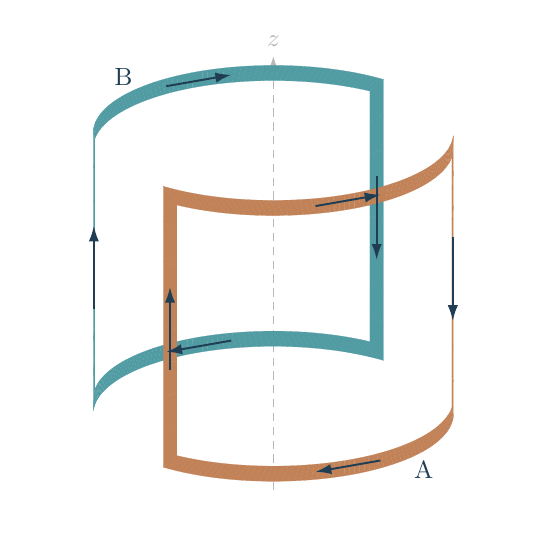
\begin{tikzpicture}[x=5.2cm,y=5.2cm,font=\small,>=Latex]
\path[use as bounding box] (-.60,-.60) rectangle (.60,.60);
\draw[gray!55,densely dashed,->] (0,-.53)--(0,.53) node[above] {$z$};
\path[fill=teal!82,draw=teal!82,line width=.06pt] (0.002470,-0.141146) -- (-0.010493,-0.141191) -- (0.005976,-0.178246) -- (0.020110,-0.178403) -- cycle;
\path[fill=teal!82,draw=teal!82,line width=.06pt] (-0.010493,-0.141191) -- (-0.023447,-0.141378) -- (-0.008163,-0.178259) -- (0.005976,-0.178246) -- cycle;
\path[fill=teal!82,draw=teal!82,line width=.06pt] (0.015430,-0.141245) -- (0.002470,-0.141146) -- (0.020110,-0.178403) -- (0.034222,-0.178730) -- cycle;
\path[fill=teal!82,draw=teal!82,line width=.06pt] (-0.023447,-0.141378) -- (-0.036380,-0.141708) -- (-0.022294,-0.178443) -- (-0.008163,-0.178259) -- cycle;
\path[fill=teal!82,draw=teal!82,line width=.06pt] (0.028378,-0.141487) -- (0.015430,-0.141245) -- (0.034222,-0.178730) -- (0.048300,-0.179227) -- cycle;
\path[fill=teal!82,draw=teal!82,line width=.06pt] (-0.036380,-0.141708) -- (-0.049282,-0.142181) -- (-0.036402,-0.178796) -- (-0.022294,-0.178443) -- cycle;
\path[fill=teal!82,draw=teal!82,line width=.06pt] (0.041300,-0.141871) -- (0.028378,-0.141487) -- (0.048300,-0.179227) -- (0.062327,-0.179893) -- cycle;
\path[fill=teal!82,draw=teal!82,line width=.06pt] (-0.049282,-0.142181) -- (-0.062140,-0.142796) -- (-0.050473,-0.179319) -- (-0.036402,-0.178796) -- cycle;
\path[fill=teal!82,draw=teal!82,line width=.06pt] (0.054187,-0.142398) -- (0.041300,-0.141871) -- (0.062327,-0.179893) -- (0.076290,-0.180728) -- cycle;
\path[fill=teal!82,draw=teal!82,line width=.06pt] (-0.062140,-0.142796) -- (-0.074945,-0.143552) -- (-0.064491,-0.180011) -- (-0.050473,-0.179319) -- cycle;
\path[fill=teal!82,draw=teal!82,line width=.06pt] (0.067026,-0.143067) -- (0.054187,-0.142398) -- (0.076290,-0.180728) -- (0.090174,-0.181730) -- cycle;
\path[fill=teal!82,draw=teal!82,line width=.06pt] (-0.074945,-0.143552) -- (-0.087685,-0.144450) -- (-0.078443,-0.180872) -- (-0.064491,-0.180011) -- cycle;
\path[fill=teal!82,draw=teal!82,line width=.06pt] (0.079808,-0.143878) -- (0.067026,-0.143067) -- (0.090174,-0.181730) -- (0.103966,-0.182898) -- cycle;
\path[fill=teal!82,draw=teal!82,line width=.06pt] (-0.087685,-0.144450) -- (-0.100349,-0.145488) -- (-0.092314,-0.181900) -- (-0.078443,-0.180872) -- cycle;
\path[fill=teal!82,draw=teal!82,line width=.06pt] (0.092520,-0.144829) -- (0.079808,-0.143878) -- (0.103966,-0.182898) -- (0.117649,-0.184232) -- cycle;
\path[fill=teal!82,draw=teal!82,line width=.06pt] (-0.100349,-0.145488) -- (-0.112926,-0.146665) -- (-0.106089,-0.183094) -- (-0.092314,-0.181900) -- cycle;
\path[fill=teal!82,draw=teal!82,line width=.06pt] (0.105152,-0.145920) -- (0.092520,-0.144829) -- (0.117649,-0.184232) -- (0.131212,-0.185731) -- cycle;
\path[fill=teal!82,draw=teal!82,line width=.06pt] (-0.112926,-0.146665) -- (-0.125405,-0.147980) -- (-0.119755,-0.184454) -- (-0.106089,-0.183094) -- cycle;
\path[fill=teal!82,draw=teal!82,line width=.06pt] (0.117693,-0.147150) -- (0.105152,-0.145920) -- (0.131212,-0.185731) -- (0.144638,-0.187391) -- cycle;
\path[fill=teal!82,draw=teal!82,line width=.06pt] (-0.125405,-0.147980) -- (-0.137774,-0.149433) -- (-0.133297,-0.185977) -- (-0.119755,-0.184454) -- cycle;
\path[fill=teal!82,draw=teal!82,line width=.06pt] (0.130131,-0.148517) -- (0.117693,-0.147150) -- (0.144638,-0.187391) -- (0.157916,-0.189213) -- cycle;
\path[fill=teal!82,draw=teal!82,line width=.06pt] (-0.137774,-0.149433) -- (-0.150025,-0.151021) -- (-0.146702,-0.187662) -- (-0.133297,-0.185977) -- cycle;
\path[fill=teal!82,draw=teal!82,line width=.06pt] (0.142457,-0.150022) -- (0.130131,-0.148517) -- (0.157916,-0.189213) -- (0.171030,-0.191193) -- cycle;
\path[fill=teal!82,draw=teal!82,line width=.06pt] (-0.150025,-0.151021) -- (-0.162145,-0.152744) -- (-0.159955,-0.189508) -- (-0.146702,-0.187662) -- cycle;
\path[fill=teal!82,draw=teal!82,line width=.06pt] (0.154659,-0.151662) -- (0.142457,-0.150022) -- (0.171030,-0.191193) -- (0.183968,-0.193330) -- cycle;
\path[fill=teal!82,draw=teal!82,line width=.06pt] (-0.162145,-0.152744) -- (-0.174124,-0.154600) -- (-0.173043,-0.191513) -- (-0.159955,-0.189508) -- cycle;
\path[fill=teal!82,draw=teal!82,line width=.06pt] (0.166726,-0.153435) -- (0.154659,-0.151662) -- (0.183968,-0.193330) -- (0.196715,-0.195621) -- cycle;
\path[fill=teal!82,draw=teal!82,line width=.06pt] (-0.174124,-0.154600) -- (-0.185952,-0.156587) -- (-0.185952,-0.193674) -- (-0.173043,-0.191513) -- cycle;
\path[fill=teal!82,draw=teal!82,line width=.06pt] (0.178649,-0.155341) -- (0.166726,-0.153435) -- (0.196715,-0.195621) -- (0.209260,-0.198065) -- cycle;
\path[fill=teal!82,draw=teal!82,line width=.06pt] (-0.185952,-0.156587) -- (-0.197619,-0.158704) -- (-0.198669,-0.195989) -- (-0.185952,-0.193674) -- cycle;
\path[fill=teal!82,draw=teal!82,line width=.06pt] (0.190417,-0.157378) -- (0.178649,-0.155341) -- (0.209260,-0.198065) -- (0.221588,-0.200659) -- cycle;
\path[fill=teal!82,draw=teal!82,line width=.06pt] (-0.197619,-0.158704) -- (-0.209114,-0.160948) -- (-0.211181,-0.198457) -- (-0.198669,-0.195989) -- cycle;
\path[fill=teal!82,draw=teal!82,line width=.06pt] (0.202020,-0.159544) -- (0.190417,-0.157378) -- (0.221588,-0.200659) -- (0.233688,-0.203400) -- cycle;
\path[fill=teal!82,draw=teal!82,line width=.06pt] (-0.209114,-0.160948) -- (-0.220428,-0.163319) -- (-0.223475,-0.201073) -- (-0.211181,-0.198457) -- cycle;
\path[fill=teal!82,draw=teal!82,line width=.06pt] (0.213447,-0.161837) -- (0.202020,-0.159544) -- (0.233688,-0.203400) -- (0.245546,-0.206285) -- cycle;
\path[fill=teal!82,draw=teal!82,line width=.06pt] (-0.220428,-0.163319) -- (-0.231550,-0.165813) -- (-0.235538,-0.203836) -- (-0.223475,-0.201073) -- cycle;
\path[fill=teal!82,draw=teal!82,line width=.06pt] (0.224689,-0.164255) -- (0.213447,-0.161837) -- (0.245546,-0.206285) -- (0.257151,-0.209311) -- cycle;
\path[fill=teal!82,draw=teal!82,line width=.06pt] (-0.231550,-0.165813) -- (-0.242471,-0.168430) -- (-0.247358,-0.206743) -- (-0.235538,-0.203836) -- cycle;
\path[fill=teal!82,draw=teal!82,line width=.06pt] (0.235736,-0.166796) -- (0.224689,-0.164255) -- (0.257151,-0.209311) -- (0.268490,-0.212475) -- cycle;
\path[fill=teal!82,draw=teal!82,line width=.06pt] (-0.242471,-0.168430) -- (-0.253182,-0.171165) -- (-0.258923,-0.209791) -- (-0.247358,-0.206743) -- cycle;
\path[fill=teal!82,draw=teal!82,line width=.06pt] (-0.253182,-0.171165) -- (-0.263673,-0.174017) -- (-0.270220,-0.212977) -- (-0.258923,-0.209791) -- cycle;
\path[fill=teal!82,draw=teal!82,line width=.06pt] (-0.263673,-0.174017) -- (-0.273936,-0.176984) -- (-0.281238,-0.216296) -- (-0.270220,-0.212977) -- cycle;
\path[fill=teal!82,draw=teal!82,line width=.06pt] (0.235736,-0.090303) -- (0.235736,-0.166796) -- (0.268490,-0.212475) -- (0.268490,-0.126711) -- cycle;
\path[fill=teal!82,draw=teal!82,line width=.06pt] (-0.273936,-0.176984) -- (-0.283960,-0.180063) -- (-0.291965,-0.219747) -- (-0.281238,-0.216296) -- cycle;
\path[fill=teal!82,draw=teal!82,line width=.06pt] (-0.283960,-0.180063) -- (-0.293738,-0.183252) -- (-0.302391,-0.223325) -- (-0.291965,-0.219747) -- cycle;
\path[fill=teal!82,draw=teal!82,line width=.06pt] (-0.293738,-0.183252) -- (-0.303261,-0.186547) -- (-0.312505,-0.227026) -- (-0.302391,-0.223325) -- cycle;
\path[fill=teal!82,draw=teal!82,line width=.06pt] (-0.303261,-0.186547) -- (-0.312521,-0.189945) -- (-0.322296,-0.230848) -- (-0.312505,-0.227026) -- cycle;
\path[fill=teal!82,draw=teal!82,line width=.06pt] (0.235736,-0.013811) -- (0.235736,-0.090303) -- (0.268490,-0.126711) -- (0.268490,-0.040946) -- cycle;
\path[fill=teal!82,draw=teal!82,line width=.06pt] (-0.312521,-0.189945) -- (-0.321509,-0.193444) -- (-0.331754,-0.234785) -- (-0.322296,-0.230848) -- cycle;
\path[fill=teal!82,draw=teal!82,line width=.06pt] (-0.321509,-0.193444) -- (-0.330219,-0.197041) -- (-0.340870,-0.238834) -- (-0.331754,-0.234785) -- cycle;
\path[fill=teal!82,draw=teal!82,line width=.06pt] (-0.330219,-0.197041) -- (-0.338642,-0.200732) -- (-0.349634,-0.242991) -- (-0.340870,-0.238834) -- cycle;
\path[fill=teal!82,draw=teal!82,line width=.06pt] (0.235736,0.062682) -- (0.235736,-0.013811) -- (0.268490,-0.040946) -- (0.268490,0.044818) -- cycle;
\path[fill=teal!82,draw=teal!82,line width=.06pt] (-0.338642,-0.200732) -- (-0.346771,-0.204515) -- (-0.358036,-0.247251) -- (-0.349634,-0.242991) -- cycle;
\path[fill=teal!82,draw=teal!82,line width=.06pt] (-0.346771,-0.204515) -- (-0.354599,-0.208386) -- (-0.366069,-0.251610) -- (-0.358036,-0.247251) -- cycle;
\path[fill=teal!82,draw=teal!82,line width=.06pt] (-0.354599,-0.208386) -- (-0.362119,-0.212341) -- (-0.373724,-0.256063) -- (-0.366069,-0.251610) -- cycle;
\path[fill=teal!82,draw=teal!82,line width=.06pt] (0.235736,0.139175) -- (0.235736,0.062682) -- (0.268490,0.044818) -- (0.268490,0.130583) -- cycle;
\path[fill=teal!82,draw=teal!82,line width=.06pt] (-0.362119,-0.212341) -- (-0.369324,-0.216378) -- (-0.380993,-0.260607) -- (-0.373724,-0.256063) -- cycle;
\path[fill=teal!82,draw=teal!82,line width=.06pt] (-0.369324,-0.216378) -- (-0.376210,-0.220493) -- (-0.387868,-0.265235) -- (-0.380993,-0.260607) -- cycle;
\path[fill=teal!82,draw=teal!82,line width=.06pt] (-0.376210,-0.220493) -- (-0.382768,-0.224681) -- (-0.394343,-0.269944) -- (-0.387868,-0.265235) -- cycle;
\path[fill=teal!82,draw=teal!82,line width=.06pt] (0.235736,0.215667) -- (0.235736,0.139175) -- (0.268490,0.130583) -- (0.268490,0.216348) -- cycle;
\path[fill=teal!82,draw=teal!82,line width=.06pt] (-0.382768,-0.224681) -- (-0.388995,-0.228941) -- (-0.400411,-0.274728) -- (-0.394343,-0.269944) -- cycle;
\path[fill=teal!82,draw=teal!82,line width=.06pt] (-0.388995,-0.228941) -- (-0.394883,-0.233267) -- (-0.406065,-0.279583) -- (-0.400411,-0.274728) -- cycle;
\path[fill=teal!82,draw=teal!82,line width=.06pt] (-0.394883,-0.233267) -- (-0.400429,-0.237656) -- (-0.411300,-0.284503) -- (-0.406065,-0.279583) -- cycle;
\path[fill=teal!82,draw=teal!82,line width=.06pt] (0.235736,0.292160) -- (0.235736,0.215667) -- (0.268490,0.216348) -- (0.268490,0.302112) -- cycle;
\path[fill=teal!82,draw=teal!82,line width=.06pt] (-0.400429,-0.237656) -- (-0.405628,-0.242105) -- (-0.416110,-0.289484) -- (-0.411300,-0.284503) -- cycle;
\path[fill=teal!82,draw=teal!82,line width=.06pt] (-0.010493,0.470751) -- (0.002470,0.470795) -- (0.020110,0.507713) -- (0.005976,0.507870) -- cycle;
\path[fill=teal!82,draw=teal!82,line width=.06pt] (-0.023447,0.470563) -- (-0.010493,0.470751) -- (0.005976,0.507870) -- (-0.008163,0.507857) -- cycle;
\path[fill=teal!82,draw=teal!82,line width=.06pt] (0.002470,0.470795) -- (0.015430,0.470696) -- (0.034222,0.507386) -- (0.020110,0.507713) -- cycle;
\path[fill=teal!82,draw=teal!82,line width=.06pt] (-0.036380,0.470233) -- (-0.023447,0.470563) -- (-0.008163,0.507857) -- (-0.022294,0.507673) -- cycle;
\path[fill=teal!82,draw=teal!82,line width=.06pt] (0.015430,0.470696) -- (0.028378,0.470454) -- (0.048300,0.506889) -- (0.034222,0.507386) -- cycle;
\path[fill=teal!82,draw=teal!82,line width=.06pt] (-0.049282,0.469760) -- (-0.036380,0.470233) -- (-0.022294,0.507673) -- (-0.036402,0.507320) -- cycle;
\path[fill=teal!82,draw=teal!82,line width=.06pt] (0.028378,0.470454) -- (0.041300,0.470070) -- (0.062327,0.506223) -- (0.048300,0.506889) -- cycle;
\path[fill=teal!82,draw=teal!82,line width=.06pt] (-0.062140,0.469146) -- (-0.049282,0.469760) -- (-0.036402,0.507320) -- (-0.050473,0.506797) -- cycle;
\path[fill=teal!82,draw=teal!82,line width=.06pt] (0.041300,0.470070) -- (0.054187,0.469543) -- (0.076290,0.505388) -- (0.062327,0.506223) -- cycle;
\path[fill=teal!82,draw=teal!82,line width=.06pt] (-0.074945,0.468389) -- (-0.062140,0.469146) -- (-0.050473,0.506797) -- (-0.064491,0.506105) -- cycle;
\path[fill=teal!82,draw=teal!82,line width=.06pt] (0.054187,0.469543) -- (0.067026,0.468874) -- (0.090174,0.504386) -- (0.076290,0.505388) -- cycle;
\path[fill=teal!82,draw=teal!82,line width=.06pt] (-0.087685,0.467491) -- (-0.074945,0.468389) -- (-0.064491,0.506105) -- (-0.078443,0.505244) -- cycle;
\path[fill=teal!82,draw=teal!82,line width=.06pt] (-0.405628,-0.242105) -- (-0.410474,-0.246609) -- (-0.420490,-0.294521) -- (-0.416110,-0.289484) -- cycle;
\path[fill=teal!82,draw=teal!82,line width=.06pt] (0.067026,0.468874) -- (0.079808,0.468064) -- (0.103966,0.503218) -- (0.090174,0.504386) -- cycle;
\path[fill=teal!82,draw=teal!82,line width=.06pt] (-0.100349,0.466454) -- (-0.087685,0.467491) -- (-0.078443,0.505244) -- (-0.092314,0.504216) -- cycle;
\path[fill=teal!82,draw=teal!82,line width=.06pt] (0.079808,0.468064) -- (0.092520,0.467112) -- (0.117649,0.501884) -- (0.103966,0.503218) -- cycle;
\path[fill=teal!82,draw=teal!82,line width=.06pt] (-0.112926,0.465277) -- (-0.100349,0.466454) -- (-0.092314,0.504216) -- (-0.106089,0.503022) -- cycle;
\path[fill=teal!82,draw=teal!82,line width=.06pt] (0.092520,0.467112) -- (0.105152,0.466022) -- (0.131212,0.500385) -- (0.117649,0.501884) -- cycle;
\path[fill=teal!82,draw=teal!82,line width=.06pt] (-0.125405,0.463961) -- (-0.112926,0.465277) -- (-0.106089,0.503022) -- (-0.119755,0.501663) -- cycle;
\path[fill=teal!82,draw=teal!82,line width=.06pt] (0.105152,0.466022) -- (0.117693,0.464792) -- (0.144638,0.498725) -- (0.131212,0.500385) -- cycle;
\path[fill=teal!82,draw=teal!82,line width=.06pt] (-0.137774,0.462509) -- (-0.125405,0.463961) -- (-0.119755,0.501663) -- (-0.133297,0.500139) -- cycle;
\path[fill=teal!82,draw=teal!82,line width=.06pt] (-0.410474,-0.246609) -- (-0.414964,-0.251164) -- (-0.424436,-0.299607) -- (-0.420490,-0.294521) -- cycle;
\path[fill=teal!82,draw=teal!82,line width=.06pt] (0.117693,0.464792) -- (0.130131,0.463424) -- (0.157916,0.496904) -- (0.144638,0.498725) -- cycle;
\path[fill=teal!82,draw=teal!82,line width=.06pt] (-0.150025,0.460920) -- (-0.137774,0.462509) -- (-0.133297,0.500139) -- (-0.146702,0.498454) -- cycle;
\path[fill=teal!82,draw=teal!82,line width=.06pt] (0.130131,0.463424) -- (0.142457,0.461920) -- (0.171030,0.494923) -- (0.157916,0.496904) -- cycle;
\path[fill=teal!82,draw=teal!82,line width=.06pt] (0.235736,0.368653) -- (0.235736,0.292160) -- (0.268490,0.302112) -- (0.268490,0.387877) -- cycle;
\path[fill=teal!82,draw=teal!82,line width=.06pt] (-0.162145,0.459198) -- (-0.150025,0.460920) -- (-0.146702,0.498454) -- (-0.159955,0.496608) -- cycle;
\path[fill=teal!82,draw=teal!82,line width=.06pt] (0.142457,0.461920) -- (0.154659,0.460280) -- (0.183968,0.492786) -- (0.171030,0.494923) -- cycle;
\path[fill=teal!82,draw=teal!82,line width=.06pt] (-0.414964,-0.251164) -- (-0.419094,-0.255767) -- (-0.427944,-0.304738) -- (-0.424436,-0.299607) -- cycle;
\path[fill=teal!82,draw=teal!82,line width=.06pt] (-0.174124,0.457342) -- (-0.162145,0.459198) -- (-0.159955,0.496608) -- (-0.173043,0.494603) -- cycle;
\path[fill=teal!82,draw=teal!82,line width=.06pt] (0.154659,0.460280) -- (0.166726,0.458506) -- (0.196715,0.490495) -- (0.183968,0.492786) -- cycle;
\path[fill=teal!82,draw=teal!82,line width=.06pt] (-0.185952,0.455355) -- (-0.174124,0.457342) -- (-0.173043,0.494603) -- (-0.185952,0.492442) -- cycle;
\path[fill=teal!82,draw=teal!82,line width=.06pt] (0.166726,0.458506) -- (0.178649,0.456600) -- (0.209260,0.488051) -- (0.196715,0.490495) -- cycle;
\path[fill=teal!82,draw=teal!82,line width=.06pt] (-0.197619,0.453238) -- (-0.185952,0.455355) -- (-0.185952,0.492442) -- (-0.198669,0.490127) -- cycle;
\path[fill=teal!82,draw=teal!82,line width=.06pt] (-0.419094,-0.255767) -- (-0.422860,-0.260414) -- (-0.431010,-0.309909) -- (-0.427944,-0.304738) -- cycle;
\path[fill=teal!82,draw=teal!82,line width=.06pt] (0.178649,0.456600) -- (0.190417,0.454563) -- (0.221588,0.485457) -- (0.209260,0.488051) -- cycle;
\path[fill=teal!82,draw=teal!82,line width=.06pt] (-0.209114,0.450993) -- (-0.197619,0.453238) -- (-0.198669,0.490127) -- (-0.211181,0.487659) -- cycle;
\path[fill=teal!82,draw=teal!82,line width=.06pt] (0.190417,0.454563) -- (0.202020,0.452397) -- (0.233688,0.482716) -- (0.221588,0.485457) -- cycle;
\path[fill=teal!82,draw=teal!82,line width=.06pt] (-0.220428,0.448622) -- (-0.209114,0.450993) -- (-0.211181,0.487659) -- (-0.223475,0.485043) -- cycle;
\path[fill=teal!82,draw=teal!82,line width=.06pt] (-0.422860,-0.260414) -- (-0.426259,-0.265100) -- (-0.433631,-0.315114) -- (-0.431010,-0.309909) -- cycle;
\path[fill=teal!82,draw=teal!82,line width=.06pt] (0.202020,0.452397) -- (0.213447,0.450104) -- (0.245546,0.479831) -- (0.233688,0.482716) -- cycle;
\path[fill=teal!82,draw=teal!82,line width=.06pt] (0.235736,0.445145) -- (0.235736,0.368653) -- (0.268490,0.387877) -- (0.268490,0.473641) -- cycle;
\path[fill=teal!82,draw=teal!82,line width=.06pt] (-0.231550,0.446128) -- (-0.220428,0.448622) -- (-0.223475,0.485043) -- (-0.235538,0.482280) -- cycle;
\path[fill=teal!82,draw=teal!82,line width=.06pt] (0.213447,0.450104) -- (0.224689,0.447686) -- (0.257151,0.476805) -- (0.245546,0.479831) -- cycle;
\path[fill=teal!82,draw=teal!82,line width=.06pt] (-0.242471,0.443512) -- (-0.231550,0.446128) -- (-0.235538,0.482280) -- (-0.247358,0.479373) -- cycle;
\path[fill=teal!82,draw=teal!82,line width=.06pt] (-0.426259,-0.265100) -- (-0.429288,-0.269822) -- (-0.435803,-0.320348) -- (-0.433631,-0.315114) -- cycle;
\path[fill=teal!82,draw=teal!82,line width=.06pt] (0.224689,0.447686) -- (0.235736,0.445145) -- (0.268490,0.473641) -- (0.257151,0.476805) -- cycle;
\path[fill=teal!82,draw=teal!82,line width=.06pt] (-0.253182,0.440776) -- (-0.242471,0.443512) -- (-0.247358,0.479373) -- (-0.258923,0.476325) -- cycle;
\path[fill=teal!82,draw=teal!82,line width=.06pt] (-0.429288,-0.269822) -- (-0.431944,-0.274575) -- (-0.437526,-0.325605) -- (-0.435803,-0.320348) -- cycle;
\path[fill=teal!82,draw=teal!82,line width=.06pt] (-0.263673,0.437924) -- (-0.253182,0.440776) -- (-0.258923,0.476325) -- (-0.270220,0.473140) -- cycle;
\path[fill=teal!82,draw=teal!82,line width=.06pt] (-0.273936,0.434957) -- (-0.263673,0.437924) -- (-0.270220,0.473140) -- (-0.281238,0.469820) -- cycle;
\path[fill=teal!82,draw=teal!82,line width=.06pt] (-0.431944,-0.274575) -- (-0.434226,-0.279355) -- (-0.438797,-0.330880) -- (-0.437526,-0.325605) -- cycle;
\path[fill=teal!82,draw=teal!82,line width=.06pt] (-0.283960,0.431878) -- (-0.273936,0.434957) -- (-0.281238,0.469820) -- (-0.291965,0.466369) -- cycle;
\path[fill=teal!82,draw=teal!82,line width=.06pt] (-0.293738,0.428690) -- (-0.283960,0.431878) -- (-0.291965,0.466369) -- (-0.302391,0.462791) -- cycle;
\path[fill=teal!82,draw=teal!82,line width=.06pt] (-0.434226,-0.279355) -- (-0.436130,-0.284159) -- (-0.439615,-0.336168) -- (-0.438797,-0.330880) -- cycle;
\path[fill=teal!82,draw=teal!82,line width=.06pt] (-0.303261,0.425395) -- (-0.293738,0.428690) -- (-0.302391,0.462791) -- (-0.312505,0.459090) -- cycle;
\path[fill=teal!82,draw=teal!82,line width=.06pt] (-0.312521,0.421996) -- (-0.303261,0.425395) -- (-0.312505,0.459090) -- (-0.322296,0.455268) -- cycle;
\path[fill=teal!82,draw=teal!82,line width=.06pt] (-0.436130,-0.284159) -- (-0.436130,-0.207666) -- (-0.439615,-0.250404) -- (-0.439615,-0.336168) -- cycle;
\path[fill=teal!82,draw=teal!82,line width=.06pt] (-0.321509,0.418497) -- (-0.312521,0.421996) -- (-0.322296,0.455268) -- (-0.331754,0.451331) -- cycle;
\path[fill=teal!82,draw=teal!82,line width=.06pt] (-0.330219,0.414900) -- (-0.321509,0.418497) -- (-0.331754,0.451331) -- (-0.340870,0.447282) -- cycle;
\path[fill=teal!82,draw=teal!82,line width=.06pt] (-0.338642,0.411209) -- (-0.330219,0.414900) -- (-0.340870,0.447282) -- (-0.349634,0.443125) -- cycle;
\path[fill=teal!82,draw=teal!82,line width=.06pt] (-0.346771,0.407426) -- (-0.338642,0.411209) -- (-0.349634,0.443125) -- (-0.358036,0.438865) -- cycle;
\path[fill=teal!82,draw=teal!82,line width=.06pt] (-0.436130,-0.207666) -- (-0.436130,-0.131174) -- (-0.439615,-0.164639) -- (-0.439615,-0.250404) -- cycle;
\path[fill=teal!82,draw=teal!82,line width=.06pt] (-0.354599,0.403555) -- (-0.346771,0.407426) -- (-0.358036,0.438865) -- (-0.366069,0.434506) -- cycle;
\path[fill=teal!82,draw=teal!82,line width=.06pt] (-0.362119,0.399600) -- (-0.354599,0.403555) -- (-0.366069,0.434506) -- (-0.373724,0.430053) -- cycle;
\path[fill=copper!82,draw=copper!82,line width=.06pt] (0.434226,-0.332586) -- (0.436130,-0.327782) -- (0.439615,-0.349948) -- (0.438797,-0.355236) -- cycle;
\path[fill=teal!82,draw=teal!82,line width=.06pt] (-0.369324,0.395563) -- (-0.362119,0.399600) -- (-0.373724,0.430053) -- (-0.380993,0.425509) -- cycle;
\path[fill=teal!82,draw=teal!82,line width=.06pt] (-0.436130,-0.131174) -- (-0.436130,-0.054681) -- (-0.439615,-0.078875) -- (-0.439615,-0.164639) -- cycle;
\path[fill=copper!82,draw=copper!82,line width=.06pt] (0.436130,-0.327782) -- (0.436130,-0.251290) -- (0.439615,-0.264183) -- (0.439615,-0.349948) -- cycle;
\path[fill=copper!82,draw=copper!82,line width=.06pt] (0.431944,-0.337366) -- (0.434226,-0.332586) -- (0.438797,-0.355236) -- (0.437526,-0.360511) -- cycle;
\path[fill=teal!82,draw=teal!82,line width=.06pt] (-0.376210,0.391449) -- (-0.369324,0.395563) -- (-0.380993,0.425509) -- (-0.387868,0.420881) -- cycle;
\path[fill=teal!82,draw=teal!82,line width=.06pt] (-0.382768,0.387260) -- (-0.376210,0.391449) -- (-0.387868,0.420881) -- (-0.394343,0.416172) -- cycle;
\path[fill=copper!82,draw=copper!82,line width=.06pt] (0.429288,-0.342119) -- (0.431944,-0.337366) -- (0.437526,-0.360511) -- (0.435803,-0.365768) -- cycle;
\path[fill=teal!82,draw=teal!82,line width=.06pt] (-0.388995,0.383001) -- (-0.382768,0.387260) -- (-0.394343,0.416172) -- (-0.400411,0.411388) -- cycle;
\path[fill=copper!82,draw=copper!82,line width=.06pt] (0.426259,-0.346841) -- (0.429288,-0.342119) -- (0.435803,-0.365768) -- (0.433631,-0.371002) -- cycle;
\path[fill=teal!82,draw=teal!82,line width=.06pt] (-0.436130,-0.054681) -- (-0.436130,0.021812) -- (-0.439615,0.006890) -- (-0.439615,-0.078875) -- cycle;
\path[fill=copper!82,draw=copper!82,line width=.06pt] (0.436130,-0.251290) -- (0.436130,-0.174797) -- (0.439615,-0.178419) -- (0.439615,-0.264183) -- cycle;
\path[fill=teal!82,draw=teal!82,line width=.06pt] (-0.394883,0.378674) -- (-0.388995,0.383001) -- (-0.400411,0.411388) -- (-0.406065,0.406533) -- cycle;
\path[fill=copper!82,draw=copper!82,line width=.06pt] (0.422860,-0.351527) -- (0.426259,-0.346841) -- (0.433631,-0.371002) -- (0.431010,-0.376207) -- cycle;
\path[fill=teal!82,draw=teal!82,line width=.06pt] (-0.400429,0.374285) -- (-0.394883,0.378674) -- (-0.406065,0.406533) -- (-0.411300,0.401613) -- cycle;
\path[fill=copper!82,draw=copper!82,line width=.06pt] (0.419094,-0.356174) -- (0.422860,-0.351527) -- (0.431010,-0.376207) -- (0.427944,-0.381378) -- cycle;
\path[fill=teal!82,draw=teal!82,line width=.06pt] (-0.405628,0.369837) -- (-0.400429,0.374285) -- (-0.411300,0.401613) -- (-0.416110,0.396632) -- cycle;
\path[fill=teal!82,draw=teal!82,line width=.06pt] (-0.436130,0.021812) -- (-0.436130,0.098304) -- (-0.439615,0.092654) -- (-0.439615,0.006890) -- cycle;
\path[fill=copper!82,draw=copper!82,line width=.06pt] (0.414964,-0.360777) -- (0.419094,-0.356174) -- (0.427944,-0.381378) -- (0.424436,-0.386509) -- cycle;
\path[fill=copper!82,draw=copper!82,line width=.06pt] (0.436130,-0.174797) -- (0.436130,-0.098304) -- (0.439615,-0.092654) -- (0.439615,-0.178419) -- cycle;
\path[fill=teal!82,draw=teal!82,line width=.06pt] (-0.410474,0.365333) -- (-0.405628,0.369837) -- (-0.416110,0.396632) -- (-0.420490,0.391595) -- cycle;
\path[fill=copper!82,draw=copper!82,line width=.06pt] (0.410474,-0.365333) -- (0.414964,-0.360777) -- (0.424436,-0.386509) -- (0.420490,-0.391595) -- cycle;
\path[fill=teal!82,draw=teal!82,line width=.06pt] (-0.414964,0.360777) -- (-0.410474,0.365333) -- (-0.420490,0.391595) -- (-0.424436,0.386509) -- cycle;
\path[fill=copper!82,draw=copper!82,line width=.06pt] (0.405628,-0.369837) -- (0.410474,-0.365333) -- (0.420490,-0.391595) -- (0.416110,-0.396632) -- cycle;
\path[fill=teal!82,draw=teal!82,line width=.06pt] (-0.436130,0.098304) -- (-0.436130,0.174797) -- (-0.439615,0.178419) -- (-0.439615,0.092654) -- cycle;
\path[fill=teal!82,draw=teal!82,line width=.06pt] (-0.419094,0.356174) -- (-0.414964,0.360777) -- (-0.424436,0.386509) -- (-0.427944,0.381378) -- cycle;
\path[fill=copper!82,draw=copper!82,line width=.06pt] (0.436130,-0.098304) -- (0.436130,-0.021812) -- (0.439615,-0.006890) -- (0.439615,-0.092654) -- cycle;
\path[fill=copper!82,draw=copper!82,line width=.06pt] (0.400429,-0.374285) -- (0.405628,-0.369837) -- (0.416110,-0.396632) -- (0.411300,-0.401613) -- cycle;
\path[fill=teal!82,draw=teal!82,line width=.06pt] (-0.422860,0.351527) -- (-0.419094,0.356174) -- (-0.427944,0.381378) -- (-0.431010,0.376207) -- cycle;
\path[fill=copper!82,draw=copper!82,line width=.06pt] (0.394883,-0.378674) -- (0.400429,-0.374285) -- (0.411300,-0.401613) -- (0.406065,-0.406533) -- cycle;
\path[fill=teal!82,draw=teal!82,line width=.06pt] (-0.426259,0.346841) -- (-0.422860,0.351527) -- (-0.431010,0.376207) -- (-0.433631,0.371002) -- cycle;
\path[fill=copper!82,draw=copper!82,line width=.06pt] (0.388995,-0.383001) -- (0.394883,-0.378674) -- (0.406065,-0.406533) -- (0.400411,-0.411388) -- cycle;
\path[fill=teal!82,draw=teal!82,line width=.06pt] (-0.436130,0.174797) -- (-0.436130,0.251290) -- (-0.439615,0.264183) -- (-0.439615,0.178419) -- cycle;
\path[fill=copper!82,draw=copper!82,line width=.06pt] (0.436130,-0.021812) -- (0.436130,0.054681) -- (0.439615,0.078875) -- (0.439615,-0.006890) -- cycle;
\path[fill=teal!82,draw=teal!82,line width=.06pt] (-0.429288,0.342119) -- (-0.426259,0.346841) -- (-0.433631,0.371002) -- (-0.435803,0.365768) -- cycle;
\path[fill=copper!82,draw=copper!82,line width=.06pt] (0.382768,-0.387260) -- (0.388995,-0.383001) -- (0.400411,-0.411388) -- (0.394343,-0.416172) -- cycle;
\path[fill=teal!82,draw=teal!82,line width=.06pt] (-0.431944,0.337366) -- (-0.429288,0.342119) -- (-0.435803,0.365768) -- (-0.437526,0.360511) -- cycle;
\path[fill=copper!82,draw=copper!82,line width=.06pt] (0.376210,-0.391449) -- (0.382768,-0.387260) -- (0.394343,-0.416172) -- (0.387868,-0.420881) -- cycle;
\path[fill=copper!82,draw=copper!82,line width=.06pt] (0.369324,-0.395563) -- (0.376210,-0.391449) -- (0.387868,-0.420881) -- (0.380993,-0.425509) -- cycle;
\path[fill=teal!82,draw=teal!82,line width=.06pt] (-0.434226,0.332586) -- (-0.431944,0.337366) -- (-0.437526,0.360511) -- (-0.438797,0.355236) -- cycle;
\path[fill=teal!82,draw=teal!82,line width=.06pt] (-0.436130,0.251290) -- (-0.436130,0.327782) -- (-0.439615,0.349948) -- (-0.439615,0.264183) -- cycle;
\path[fill=copper!82,draw=copper!82,line width=.06pt] (0.436130,0.054681) -- (0.436130,0.131174) -- (0.439615,0.164639) -- (0.439615,0.078875) -- cycle;
\path[fill=copper!82,draw=copper!82,line width=.06pt] (0.362119,-0.399600) -- (0.369324,-0.395563) -- (0.380993,-0.425509) -- (0.373724,-0.430053) -- cycle;
\path[fill=teal!82,draw=teal!82,line width=.06pt] (-0.436130,0.327782) -- (-0.434226,0.332586) -- (-0.438797,0.355236) -- (-0.439615,0.349948) -- cycle;
\path[fill=copper!82,draw=copper!82,line width=.06pt] (0.354599,-0.403555) -- (0.362119,-0.399600) -- (0.373724,-0.430053) -- (0.366069,-0.434506) -- cycle;
\path[fill=copper!82,draw=copper!82,line width=.06pt] (0.346771,-0.407426) -- (0.354599,-0.403555) -- (0.366069,-0.434506) -- (0.358036,-0.438865) -- cycle;
\path[fill=copper!82,draw=copper!82,line width=.06pt] (0.436130,0.131174) -- (0.436130,0.207666) -- (0.439615,0.250404) -- (0.439615,0.164639) -- cycle;
\path[fill=copper!82,draw=copper!82,line width=.06pt] (0.338642,-0.411209) -- (0.346771,-0.407426) -- (0.358036,-0.438865) -- (0.349634,-0.443125) -- cycle;
\path[fill=copper!82,draw=copper!82,line width=.06pt] (0.330219,-0.414900) -- (0.338642,-0.411209) -- (0.349634,-0.443125) -- (0.340870,-0.447282) -- cycle;
\path[fill=copper!82,draw=copper!82,line width=.06pt] (0.321509,-0.418497) -- (0.330219,-0.414900) -- (0.340870,-0.447282) -- (0.331754,-0.451331) -- cycle;
\path[fill=copper!82,draw=copper!82,line width=.06pt] (0.312521,-0.421996) -- (0.321509,-0.418497) -- (0.331754,-0.451331) -- (0.322296,-0.455268) -- cycle;
\path[fill=copper!82,draw=copper!82,line width=.06pt] (0.436130,0.207666) -- (0.436130,0.284159) -- (0.439615,0.336168) -- (0.439615,0.250404) -- cycle;
\path[fill=copper!82,draw=copper!82,line width=.06pt] (0.303261,-0.425395) -- (0.312521,-0.421996) -- (0.322296,-0.455268) -- (0.312505,-0.459090) -- cycle;
\path[fill=copper!82,draw=copper!82,line width=.06pt] (0.293738,-0.428690) -- (0.303261,-0.425395) -- (0.312505,-0.459090) -- (0.302391,-0.462791) -- cycle;
\path[fill=copper!82,draw=copper!82,line width=.06pt] (0.436130,0.284159) -- (0.434226,0.279355) -- (0.438797,0.330880) -- (0.439615,0.336168) -- cycle;
\path[fill=copper!82,draw=copper!82,line width=.06pt] (0.283960,-0.431878) -- (0.293738,-0.428690) -- (0.302391,-0.462791) -- (0.291965,-0.466369) -- cycle;
\path[fill=copper!82,draw=copper!82,line width=.06pt] (0.273936,-0.434957) -- (0.283960,-0.431878) -- (0.291965,-0.466369) -- (0.281238,-0.469820) -- cycle;
\path[fill=copper!82,draw=copper!82,line width=.06pt] (0.434226,0.279355) -- (0.431944,0.274575) -- (0.437526,0.325605) -- (0.438797,0.330880) -- cycle;
\path[fill=copper!82,draw=copper!82,line width=.06pt] (0.263673,-0.437924) -- (0.273936,-0.434957) -- (0.281238,-0.469820) -- (0.270220,-0.473140) -- cycle;
\path[fill=copper!82,draw=copper!82,line width=.06pt] (0.253182,-0.440776) -- (0.263673,-0.437924) -- (0.270220,-0.473140) -- (0.258923,-0.476325) -- cycle;
\path[fill=copper!82,draw=copper!82,line width=.06pt] (0.431944,0.274575) -- (0.429288,0.269822) -- (0.435803,0.320348) -- (0.437526,0.325605) -- cycle;
\path[fill=copper!82,draw=copper!82,line width=.06pt] (0.242471,-0.443512) -- (0.253182,-0.440776) -- (0.258923,-0.476325) -- (0.247358,-0.479373) -- cycle;
\path[fill=copper!82,draw=copper!82,line width=.06pt] (-0.235736,-0.445145) -- (-0.224689,-0.447686) -- (-0.257151,-0.476805) -- (-0.268490,-0.473641) -- cycle;
\path[fill=copper!82,draw=copper!82,line width=.06pt] (0.429288,0.269822) -- (0.426259,0.265100) -- (0.433631,0.315114) -- (0.435803,0.320348) -- cycle;
\path[fill=copper!82,draw=copper!82,line width=.06pt] (0.231550,-0.446128) -- (0.242471,-0.443512) -- (0.247358,-0.479373) -- (0.235538,-0.482280) -- cycle;
\path[fill=copper!82,draw=copper!82,line width=.06pt] (-0.224689,-0.447686) -- (-0.213447,-0.450104) -- (-0.245546,-0.479831) -- (-0.257151,-0.476805) -- cycle;
\path[fill=copper!82,draw=copper!82,line width=.06pt] (0.220428,-0.448622) -- (0.231550,-0.446128) -- (0.235538,-0.482280) -- (0.223475,-0.485043) -- cycle;
\path[fill=copper!82,draw=copper!82,line width=.06pt] (-0.235736,-0.368653) -- (-0.235736,-0.445145) -- (-0.268490,-0.473641) -- (-0.268490,-0.387877) -- cycle;
\path[fill=copper!82,draw=copper!82,line width=.06pt] (-0.213447,-0.450104) -- (-0.202020,-0.452397) -- (-0.233688,-0.482716) -- (-0.245546,-0.479831) -- cycle;
\path[fill=copper!82,draw=copper!82,line width=.06pt] (0.426259,0.265100) -- (0.422860,0.260414) -- (0.431010,0.309909) -- (0.433631,0.315114) -- cycle;
\path[fill=copper!82,draw=copper!82,line width=.06pt] (0.209114,-0.450993) -- (0.220428,-0.448622) -- (0.223475,-0.485043) -- (0.211181,-0.487659) -- cycle;
\path[fill=copper!82,draw=copper!82,line width=.06pt] (-0.202020,-0.452397) -- (-0.190417,-0.454563) -- (-0.221588,-0.485457) -- (-0.233688,-0.482716) -- cycle;
\path[fill=copper!82,draw=copper!82,line width=.06pt] (0.197619,-0.453238) -- (0.209114,-0.450993) -- (0.211181,-0.487659) -- (0.198669,-0.490127) -- cycle;
\path[fill=copper!82,draw=copper!82,line width=.06pt] (-0.190417,-0.454563) -- (-0.178649,-0.456600) -- (-0.209260,-0.488051) -- (-0.221588,-0.485457) -- cycle;
\path[fill=copper!82,draw=copper!82,line width=.06pt] (0.422860,0.260414) -- (0.419094,0.255767) -- (0.427944,0.304738) -- (0.431010,0.309909) -- cycle;
\path[fill=copper!82,draw=copper!82,line width=.06pt] (0.185952,-0.455355) -- (0.197619,-0.453238) -- (0.198669,-0.490127) -- (0.185952,-0.492442) -- cycle;
\path[fill=copper!82,draw=copper!82,line width=.06pt] (-0.178649,-0.456600) -- (-0.166726,-0.458506) -- (-0.196715,-0.490495) -- (-0.209260,-0.488051) -- cycle;
\path[fill=copper!82,draw=copper!82,line width=.06pt] (0.174124,-0.457342) -- (0.185952,-0.455355) -- (0.185952,-0.492442) -- (0.173043,-0.494603) -- cycle;
\path[fill=copper!82,draw=copper!82,line width=.06pt] (-0.166726,-0.458506) -- (-0.154659,-0.460280) -- (-0.183968,-0.492786) -- (-0.196715,-0.490495) -- cycle;
\path[fill=copper!82,draw=copper!82,line width=.06pt] (0.162145,-0.459198) -- (0.174124,-0.457342) -- (0.173043,-0.494603) -- (0.159955,-0.496608) -- cycle;
\path[fill=copper!82,draw=copper!82,line width=.06pt] (0.419094,0.255767) -- (0.414964,0.251164) -- (0.424436,0.299607) -- (0.427944,0.304738) -- cycle;
\path[fill=copper!82,draw=copper!82,line width=.06pt] (-0.154659,-0.460280) -- (-0.142457,-0.461920) -- (-0.171030,-0.494923) -- (-0.183968,-0.492786) -- cycle;
\path[fill=copper!82,draw=copper!82,line width=.06pt] (0.150025,-0.460920) -- (0.162145,-0.459198) -- (0.159955,-0.496608) -- (0.146702,-0.498454) -- cycle;
\path[fill=copper!82,draw=copper!82,line width=.06pt] (-0.235736,-0.292160) -- (-0.235736,-0.368653) -- (-0.268490,-0.387877) -- (-0.268490,-0.302112) -- cycle;
\path[fill=copper!82,draw=copper!82,line width=.06pt] (-0.142457,-0.461920) -- (-0.130131,-0.463424) -- (-0.157916,-0.496904) -- (-0.171030,-0.494923) -- cycle;
\path[fill=copper!82,draw=copper!82,line width=.06pt] (0.137774,-0.462509) -- (0.150025,-0.460920) -- (0.146702,-0.498454) -- (0.133297,-0.500139) -- cycle;
\path[fill=copper!82,draw=copper!82,line width=.06pt] (-0.130131,-0.463424) -- (-0.117693,-0.464792) -- (-0.144638,-0.498725) -- (-0.157916,-0.496904) -- cycle;
\path[fill=copper!82,draw=copper!82,line width=.06pt] (0.414964,0.251164) -- (0.410474,0.246609) -- (0.420490,0.294521) -- (0.424436,0.299607) -- cycle;
\path[fill=copper!82,draw=copper!82,line width=.06pt] (0.125405,-0.463961) -- (0.137774,-0.462509) -- (0.133297,-0.500139) -- (0.119755,-0.501663) -- cycle;
\path[fill=copper!82,draw=copper!82,line width=.06pt] (-0.117693,-0.464792) -- (-0.105152,-0.466022) -- (-0.131212,-0.500385) -- (-0.144638,-0.498725) -- cycle;
\path[fill=copper!82,draw=copper!82,line width=.06pt] (0.112926,-0.465277) -- (0.125405,-0.463961) -- (0.119755,-0.501663) -- (0.106089,-0.503022) -- cycle;
\path[fill=copper!82,draw=copper!82,line width=.06pt] (-0.105152,-0.466022) -- (-0.092520,-0.467112) -- (-0.117649,-0.501884) -- (-0.131212,-0.500385) -- cycle;
\path[fill=copper!82,draw=copper!82,line width=.06pt] (0.100349,-0.466454) -- (0.112926,-0.465277) -- (0.106089,-0.503022) -- (0.092314,-0.504216) -- cycle;
\path[fill=copper!82,draw=copper!82,line width=.06pt] (-0.092520,-0.467112) -- (-0.079808,-0.468064) -- (-0.103966,-0.503218) -- (-0.117649,-0.501884) -- cycle;
\path[fill=copper!82,draw=copper!82,line width=.06pt] (0.087685,-0.467491) -- (0.100349,-0.466454) -- (0.092314,-0.504216) -- (0.078443,-0.505244) -- cycle;
\path[fill=copper!82,draw=copper!82,line width=.06pt] (-0.079808,-0.468064) -- (-0.067026,-0.468874) -- (-0.090174,-0.504386) -- (-0.103966,-0.503218) -- cycle;
\path[fill=copper!82,draw=copper!82,line width=.06pt] (0.410474,0.246609) -- (0.405628,0.242105) -- (0.416110,0.289484) -- (0.420490,0.294521) -- cycle;
\path[fill=copper!82,draw=copper!82,line width=.06pt] (0.074945,-0.468389) -- (0.087685,-0.467491) -- (0.078443,-0.505244) -- (0.064491,-0.506105) -- cycle;
\path[fill=copper!82,draw=copper!82,line width=.06pt] (-0.067026,-0.468874) -- (-0.054187,-0.469543) -- (-0.076290,-0.505388) -- (-0.090174,-0.504386) -- cycle;
\path[fill=copper!82,draw=copper!82,line width=.06pt] (0.062140,-0.469146) -- (0.074945,-0.468389) -- (0.064491,-0.506105) -- (0.050473,-0.506797) -- cycle;
\path[fill=copper!82,draw=copper!82,line width=.06pt] (-0.054187,-0.469543) -- (-0.041300,-0.470070) -- (-0.062327,-0.506223) -- (-0.076290,-0.505388) -- cycle;
\path[fill=copper!82,draw=copper!82,line width=.06pt] (0.049282,-0.469760) -- (0.062140,-0.469146) -- (0.050473,-0.506797) -- (0.036402,-0.507320) -- cycle;
\path[fill=copper!82,draw=copper!82,line width=.06pt] (-0.041300,-0.470070) -- (-0.028378,-0.470454) -- (-0.048300,-0.506889) -- (-0.062327,-0.506223) -- cycle;
\path[fill=copper!82,draw=copper!82,line width=.06pt] (0.036380,-0.470233) -- (0.049282,-0.469760) -- (0.036402,-0.507320) -- (0.022294,-0.507673) -- cycle;
\path[fill=copper!82,draw=copper!82,line width=.06pt] (-0.028378,-0.470454) -- (-0.015430,-0.470696) -- (-0.034222,-0.507386) -- (-0.048300,-0.506889) -- cycle;
\path[fill=copper!82,draw=copper!82,line width=.06pt] (0.023447,-0.470563) -- (0.036380,-0.470233) -- (0.022294,-0.507673) -- (0.008163,-0.507857) -- cycle;
\path[fill=copper!82,draw=copper!82,line width=.06pt] (-0.015430,-0.470696) -- (-0.002470,-0.470795) -- (-0.020110,-0.507713) -- (-0.034222,-0.507386) -- cycle;
\path[fill=copper!82,draw=copper!82,line width=.06pt] (0.010493,-0.470751) -- (0.023447,-0.470563) -- (0.008163,-0.507857) -- (-0.005976,-0.507870) -- cycle;
\path[fill=copper!82,draw=copper!82,line width=.06pt] (-0.002470,-0.470795) -- (0.010493,-0.470751) -- (-0.005976,-0.507870) -- (-0.020110,-0.507713) -- cycle;
\path[fill=copper!82,draw=copper!82,line width=.06pt] (0.405628,0.242105) -- (0.400429,0.237656) -- (0.411300,0.284503) -- (0.416110,0.289484) -- cycle;
\path[fill=copper!82,draw=copper!82,line width=.06pt] (-0.235736,-0.215667) -- (-0.235736,-0.292160) -- (-0.268490,-0.302112) -- (-0.268490,-0.216348) -- cycle;
\path[fill=copper!82,draw=copper!82,line width=.06pt] (0.400429,0.237656) -- (0.394883,0.233267) -- (0.406065,0.279583) -- (0.411300,0.284503) -- cycle;
\path[fill=copper!82,draw=copper!82,line width=.06pt] (0.394883,0.233267) -- (0.388995,0.228941) -- (0.400411,0.274728) -- (0.406065,0.279583) -- cycle;
\path[fill=copper!82,draw=copper!82,line width=.06pt] (0.388995,0.228941) -- (0.382768,0.224681) -- (0.394343,0.269944) -- (0.400411,0.274728) -- cycle;
\path[fill=copper!82,draw=copper!82,line width=.06pt] (-0.235736,-0.139175) -- (-0.235736,-0.215667) -- (-0.268490,-0.216348) -- (-0.268490,-0.130583) -- cycle;
\path[fill=copper!82,draw=copper!82,line width=.06pt] (0.382768,0.224681) -- (0.376210,0.220493) -- (0.387868,0.265235) -- (0.394343,0.269944) -- cycle;
\path[fill=copper!82,draw=copper!82,line width=.06pt] (0.376210,0.220493) -- (0.369324,0.216378) -- (0.380993,0.260607) -- (0.387868,0.265235) -- cycle;
\path[fill=copper!82,draw=copper!82,line width=.06pt] (0.369324,0.216378) -- (0.362119,0.212341) -- (0.373724,0.256063) -- (0.380993,0.260607) -- cycle;
\path[fill=copper!82,draw=copper!82,line width=.06pt] (-0.235736,-0.062682) -- (-0.235736,-0.139175) -- (-0.268490,-0.130583) -- (-0.268490,-0.044818) -- cycle;
\path[fill=copper!82,draw=copper!82,line width=.06pt] (0.362119,0.212341) -- (0.354599,0.208386) -- (0.366069,0.251610) -- (0.373724,0.256063) -- cycle;
\path[fill=copper!82,draw=copper!82,line width=.06pt] (0.354599,0.208386) -- (0.346771,0.204515) -- (0.358036,0.247251) -- (0.366069,0.251610) -- cycle;
\path[fill=copper!82,draw=copper!82,line width=.06pt] (0.346771,0.204515) -- (0.338642,0.200732) -- (0.349634,0.242991) -- (0.358036,0.247251) -- cycle;
\path[fill=copper!82,draw=copper!82,line width=.06pt] (-0.235736,0.013811) -- (-0.235736,-0.062682) -- (-0.268490,-0.044818) -- (-0.268490,0.040946) -- cycle;
\path[fill=copper!82,draw=copper!82,line width=.06pt] (0.338642,0.200732) -- (0.330219,0.197041) -- (0.340870,0.238834) -- (0.349634,0.242991) -- cycle;
\path[fill=copper!82,draw=copper!82,line width=.06pt] (0.330219,0.197041) -- (0.321509,0.193444) -- (0.331754,0.234785) -- (0.340870,0.238834) -- cycle;
\path[fill=copper!82,draw=copper!82,line width=.06pt] (0.321509,0.193444) -- (0.312521,0.189945) -- (0.322296,0.230848) -- (0.331754,0.234785) -- cycle;
\path[fill=copper!82,draw=copper!82,line width=.06pt] (-0.235736,0.090303) -- (-0.235736,0.013811) -- (-0.268490,0.040946) -- (-0.268490,0.126711) -- cycle;
\path[fill=copper!82,draw=copper!82,line width=.06pt] (0.312521,0.189945) -- (0.303261,0.186547) -- (0.312505,0.227026) -- (0.322296,0.230848) -- cycle;
\path[fill=copper!82,draw=copper!82,line width=.06pt] (0.303261,0.186547) -- (0.293738,0.183252) -- (0.302391,0.223325) -- (0.312505,0.227026) -- cycle;
\path[fill=copper!82,draw=copper!82,line width=.06pt] (0.293738,0.183252) -- (0.283960,0.180063) -- (0.291965,0.219747) -- (0.302391,0.223325) -- cycle;
\path[fill=copper!82,draw=copper!82,line width=.06pt] (0.283960,0.180063) -- (0.273936,0.176984) -- (0.281238,0.216296) -- (0.291965,0.219747) -- cycle;
\path[fill=copper!82,draw=copper!82,line width=.06pt] (-0.235736,0.166796) -- (-0.235736,0.090303) -- (-0.268490,0.126711) -- (-0.268490,0.212475) -- cycle;
\path[fill=copper!82,draw=copper!82,line width=.06pt] (0.273936,0.176984) -- (0.263673,0.174017) -- (0.270220,0.212977) -- (0.281238,0.216296) -- cycle;
\path[fill=copper!82,draw=copper!82,line width=.06pt] (0.263673,0.174017) -- (0.253182,0.171165) -- (0.258923,0.209791) -- (0.270220,0.212977) -- cycle;
\path[fill=copper!82,draw=copper!82,line width=.06pt] (0.253182,0.171165) -- (0.242471,0.168430) -- (0.247358,0.206743) -- (0.258923,0.209791) -- cycle;
\path[fill=copper!82,draw=copper!82,line width=.06pt] (-0.224689,0.164255) -- (-0.235736,0.166796) -- (-0.268490,0.212475) -- (-0.257151,0.209311) -- cycle;
\path[fill=copper!82,draw=copper!82,line width=.06pt] (0.242471,0.168430) -- (0.231550,0.165813) -- (0.235538,0.203836) -- (0.247358,0.206743) -- cycle;
\path[fill=copper!82,draw=copper!82,line width=.06pt] (-0.213447,0.161837) -- (-0.224689,0.164255) -- (-0.257151,0.209311) -- (-0.245546,0.206285) -- cycle;
\path[fill=copper!82,draw=copper!82,line width=.06pt] (0.231550,0.165813) -- (0.220428,0.163319) -- (0.223475,0.201073) -- (0.235538,0.203836) -- cycle;
\path[fill=copper!82,draw=copper!82,line width=.06pt] (-0.202020,0.159544) -- (-0.213447,0.161837) -- (-0.245546,0.206285) -- (-0.233688,0.203400) -- cycle;
\path[fill=copper!82,draw=copper!82,line width=.06pt] (0.220428,0.163319) -- (0.209114,0.160948) -- (0.211181,0.198457) -- (0.223475,0.201073) -- cycle;
\path[fill=copper!82,draw=copper!82,line width=.06pt] (-0.190417,0.157378) -- (-0.202020,0.159544) -- (-0.233688,0.203400) -- (-0.221588,0.200659) -- cycle;
\path[fill=copper!82,draw=copper!82,line width=.06pt] (0.209114,0.160948) -- (0.197619,0.158704) -- (0.198669,0.195989) -- (0.211181,0.198457) -- cycle;
\path[fill=copper!82,draw=copper!82,line width=.06pt] (-0.178649,0.155341) -- (-0.190417,0.157378) -- (-0.221588,0.200659) -- (-0.209260,0.198065) -- cycle;
\path[fill=copper!82,draw=copper!82,line width=.06pt] (0.197619,0.158704) -- (0.185952,0.156587) -- (0.185952,0.193674) -- (0.198669,0.195989) -- cycle;
\path[fill=copper!82,draw=copper!82,line width=.06pt] (-0.166726,0.153435) -- (-0.178649,0.155341) -- (-0.209260,0.198065) -- (-0.196715,0.195621) -- cycle;
\path[fill=copper!82,draw=copper!82,line width=.06pt] (0.185952,0.156587) -- (0.174124,0.154600) -- (0.173043,0.191513) -- (0.185952,0.193674) -- cycle;
\path[fill=copper!82,draw=copper!82,line width=.06pt] (-0.154659,0.151662) -- (-0.166726,0.153435) -- (-0.196715,0.195621) -- (-0.183968,0.193330) -- cycle;
\path[fill=copper!82,draw=copper!82,line width=.06pt] (0.174124,0.154600) -- (0.162145,0.152744) -- (0.159955,0.189508) -- (0.173043,0.191513) -- cycle;
\path[fill=copper!82,draw=copper!82,line width=.06pt] (-0.142457,0.150022) -- (-0.154659,0.151662) -- (-0.183968,0.193330) -- (-0.171030,0.191193) -- cycle;
\path[fill=copper!82,draw=copper!82,line width=.06pt] (0.162145,0.152744) -- (0.150025,0.151021) -- (0.146702,0.187662) -- (0.159955,0.189508) -- cycle;
\path[fill=copper!82,draw=copper!82,line width=.06pt] (-0.130131,0.148517) -- (-0.142457,0.150022) -- (-0.171030,0.191193) -- (-0.157916,0.189213) -- cycle;
\path[fill=copper!82,draw=copper!82,line width=.06pt] (0.150025,0.151021) -- (0.137774,0.149433) -- (0.133297,0.185977) -- (0.146702,0.187662) -- cycle;
\path[fill=copper!82,draw=copper!82,line width=.06pt] (-0.117693,0.147150) -- (-0.130131,0.148517) -- (-0.157916,0.189213) -- (-0.144638,0.187391) -- cycle;
\path[fill=copper!82,draw=copper!82,line width=.06pt] (0.137774,0.149433) -- (0.125405,0.147980) -- (0.119755,0.184454) -- (0.133297,0.185977) -- cycle;
\path[fill=copper!82,draw=copper!82,line width=.06pt] (-0.105152,0.145920) -- (-0.117693,0.147150) -- (-0.144638,0.187391) -- (-0.131212,0.185731) -- cycle;
\path[fill=copper!82,draw=copper!82,line width=.06pt] (0.125405,0.147980) -- (0.112926,0.146665) -- (0.106089,0.183094) -- (0.119755,0.184454) -- cycle;
\path[fill=copper!82,draw=copper!82,line width=.06pt] (-0.092520,0.144829) -- (-0.105152,0.145920) -- (-0.131212,0.185731) -- (-0.117649,0.184232) -- cycle;
\path[fill=copper!82,draw=copper!82,line width=.06pt] (0.112926,0.146665) -- (0.100349,0.145488) -- (0.092314,0.181900) -- (0.106089,0.183094) -- cycle;
\path[fill=copper!82,draw=copper!82,line width=.06pt] (-0.079808,0.143878) -- (-0.092520,0.144829) -- (-0.117649,0.184232) -- (-0.103966,0.182898) -- cycle;
\path[fill=copper!82,draw=copper!82,line width=.06pt] (0.100349,0.145488) -- (0.087685,0.144450) -- (0.078443,0.180872) -- (0.092314,0.181900) -- cycle;
\path[fill=copper!82,draw=copper!82,line width=.06pt] (-0.067026,0.143067) -- (-0.079808,0.143878) -- (-0.103966,0.182898) -- (-0.090174,0.181730) -- cycle;
\path[fill=copper!82,draw=copper!82,line width=.06pt] (0.087685,0.144450) -- (0.074945,0.143552) -- (0.064491,0.180011) -- (0.078443,0.180872) -- cycle;
\path[fill=copper!82,draw=copper!82,line width=.06pt] (-0.054187,0.142398) -- (-0.067026,0.143067) -- (-0.090174,0.181730) -- (-0.076290,0.180728) -- cycle;
\path[fill=copper!82,draw=copper!82,line width=.06pt] (0.074945,0.143552) -- (0.062140,0.142796) -- (0.050473,0.179319) -- (0.064491,0.180011) -- cycle;
\path[fill=copper!82,draw=copper!82,line width=.06pt] (-0.041300,0.141871) -- (-0.054187,0.142398) -- (-0.076290,0.180728) -- (-0.062327,0.179893) -- cycle;
\path[fill=copper!82,draw=copper!82,line width=.06pt] (0.062140,0.142796) -- (0.049282,0.142181) -- (0.036402,0.178796) -- (0.050473,0.179319) -- cycle;
\path[fill=copper!82,draw=copper!82,line width=.06pt] (-0.028378,0.141487) -- (-0.041300,0.141871) -- (-0.062327,0.179893) -- (-0.048300,0.179227) -- cycle;
\path[fill=copper!82,draw=copper!82,line width=.06pt] (0.049282,0.142181) -- (0.036380,0.141708) -- (0.022294,0.178443) -- (0.036402,0.178796) -- cycle;
\path[fill=copper!82,draw=copper!82,line width=.06pt] (-0.015430,0.141245) -- (-0.028378,0.141487) -- (-0.048300,0.179227) -- (-0.034222,0.178730) -- cycle;
\path[fill=copper!82,draw=copper!82,line width=.06pt] (0.036380,0.141708) -- (0.023447,0.141378) -- (0.008163,0.178259) -- (0.022294,0.178443) -- cycle;
\path[fill=copper!82,draw=copper!82,line width=.06pt] (-0.002470,0.141146) -- (-0.015430,0.141245) -- (-0.034222,0.178730) -- (-0.020110,0.178403) -- cycle;
\path[fill=copper!82,draw=copper!82,line width=.06pt] (0.023447,0.141378) -- (0.010493,0.141191) -- (-0.005976,0.178246) -- (0.008163,0.178259) -- cycle;
\path[fill=copper!82,draw=copper!82,line width=.06pt] (0.010493,0.141191) -- (-0.002470,0.141146) -- (-0.020110,0.178403) -- (-0.005976,0.178246) -- cycle;
\draw[navy,line width=.7pt,-{Latex[length=2mm,width=1.3mm]}] (0.438326,0.087625) -- (0.438326,-0.116356);
\draw[navy,line width=.7pt,-{Latex[length=2mm,width=1.3mm]}] (-0.252374,-0.237009) -- (-0.252374,-0.033028);
\draw[navy,line width=.7pt,-{Latex[length=2mm,width=1.3mm]}] (0.103021,0.164269) -- (0.261470,0.191947);
\draw[navy,line width=.7pt,-{Latex[length=2mm,width=1.3mm]}] (0.261470,-0.457081) -- (0.103021,-0.484760);
\draw[navy,line width=.7pt,-{Latex[length=2mm,width=1.3mm]}] (-0.438326,-0.087625) -- (-0.438326,0.116356);
\draw[navy,line width=.7pt,-{Latex[length=2mm,width=1.3mm]}] (0.252374,0.237009) -- (0.252374,0.033028);
\draw[navy,line width=.7pt,-{Latex[length=2mm,width=1.3mm]}] (-0.261470,0.457081) -- (-0.103021,0.484760);
\draw[navy,line width=.7pt,-{Latex[length=2mm,width=1.3mm]}] (-0.103021,-0.164269) -- (-0.261470,-0.191947);
\node[navy,anchor=west] at (.32,-.48) {A};
\node[navy,anchor=east] at (-.32,.48) {B};
\end{tikzpicture}
\par\small 三维有限带宽闭合回路
\end{minipage}\hfill
\begin{minipage}[t]{.49\linewidth}\centering\vspace{0pt}
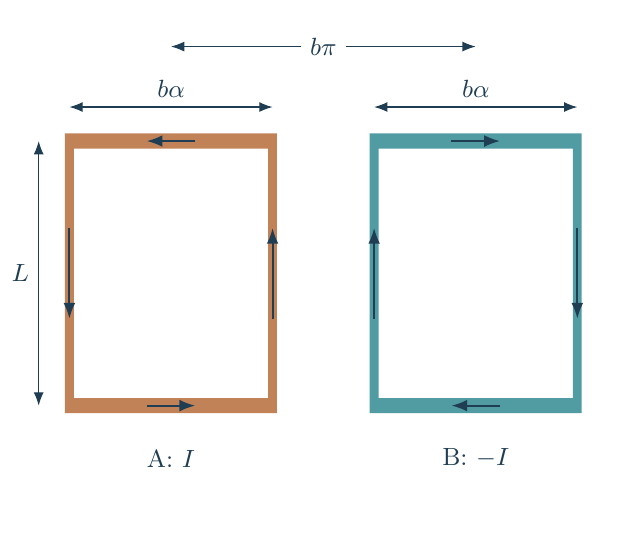
\begin{tikzpicture}[x=2.8cm,y=4.8cm,font=\small,>=Latex]
\path[use as bounding box] (-.65,-.65) rectangle (1.90,.65);
\path[fill=copper!82,even odd rule] (-0.480767,-0.370000) rectangle (0.480767,0.370000) (-0.440767,-0.330000) rectangle (0.440767,0.330000);
\draw[navy,line width=.7pt,-{Latex[length=2mm]}] (-0.460767,0.120000) -- (-0.460767,-0.120000);
\draw[navy,line width=.7pt,-{Latex[length=2mm]}] (0.460767,-0.120000) -- (0.460767,0.120000);
\draw[navy,line width=.7pt,-{Latex[length=2mm]}] (0.110000,0.350000) -- (-0.110000,0.350000);
\draw[navy,line width=.7pt,-{Latex[length=2mm]}] (-0.110000,-0.350000) -- (0.110000,-0.350000);
\draw[navy,thin,<->] (-0.460767,.44)--(0.460767,.44) node[midway,above] {$b\alpha$};
\node[navy] at (0.000000,-.49) {A: $I$};
\path[fill=teal!82,even odd rule] (0.901534,-0.370000) rectangle (1.863068,0.370000) (0.941534,-0.330000) rectangle (1.823068,0.330000);
\draw[navy,line width=.7pt,-{Latex[length=2mm]}] (0.921534,-0.120000) -- (0.921534,0.120000);
\draw[navy,line width=.7pt,-{Latex[length=2mm]}] (1.843068,0.120000) -- (1.843068,-0.120000);
\draw[navy,line width=.7pt,-{Latex[length=2mm]}] (1.272301,0.350000) -- (1.492301,0.350000);
\draw[navy,line width=.7pt,-{Latex[length=2mm]}] (1.492301,-0.350000) -- (1.272301,-0.350000);
\draw[navy,thin,<->] (0.921534,.44)--(1.843068,.44) node[midway,above] {$b\alpha$};
\node[navy] at (1.382301,-.49) {B: $-I$};
\draw[navy,thin,<->] (0,.60)--(1.382301,.60) node[midway,fill=white] {$b\pi$};
\draw[navy,thin,<->] (-.60,-.35)--(-.60,.35) node[midway,left] {$L$};
\end{tikzpicture}
\par\small 圆柱展开面：横向为 $b\phi$，竖向为 $z$
\end{minipage}
\par\smallskip\small A、B 的中心角相差 $\pi$，相同鞍形参考方向下 $I_A=I$、$I_B=-I$。
\par\small $b=0.44$ m，$L=0.70$ m，$L_{\text{宽}}=0.04$ m，$\alpha=120^\circ=2\pi/3$ rad；箭头为零整体相位、正方向时的瞬时参考电流。
% END GENERATED: double_saddle
}

\newcommand{\AntennaFigureG}{%
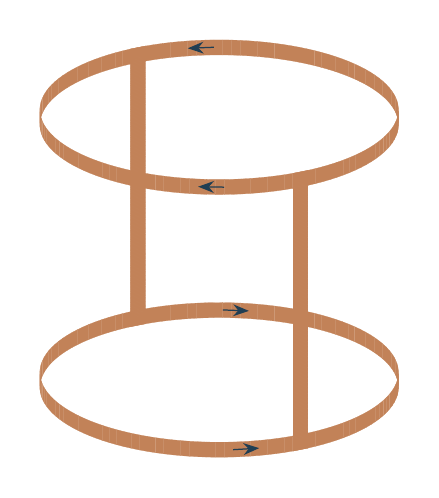
\begin{tikzpicture}[x=5.17475cm,y=5.17475cm]
\path[use as bounding box] (-0.469911,-0.542102) rectangle (0.469911,0.542102);
\path[fill=copper!82,draw=copper!82,line width=.08pt] (0.012763,0.169521) -- (-0.008834,0.169483) -- (-0.008834,0.132641) -- (0.012763,0.132678) -- cycle;
\path[fill=copper!82,draw=copper!82,line width=.08pt] (-0.008834,0.169483) -- (-0.030408,0.169858) -- (-0.030408,0.133016) -- (-0.008834,0.132641) -- cycle;
\path[fill=copper!82,draw=copper!82,line width=.08pt] (0.034328,0.169971) -- (0.012763,0.169521) -- (0.012763,0.132678) -- (0.034328,0.133128) -- cycle;
\path[fill=copper!82,draw=copper!82,line width=.08pt] (-0.030408,0.169858) -- (-0.051910,0.170645) -- (-0.051910,0.133803) -- (-0.030408,0.133016) -- cycle;
\path[fill=copper!82,draw=copper!82,line width=.08pt] (0.055810,0.170832) -- (0.034328,0.169971) -- (0.034328,0.133128) -- (0.055810,0.133990) -- cycle;
\path[fill=copper!82,draw=copper!82,line width=.08pt] (-0.051910,0.170645) -- (-0.073286,0.171842) -- (-0.073286,0.135000) -- (-0.051910,0.133803) -- cycle;
\path[fill=copper!82,draw=copper!82,line width=.08pt] (0.077159,0.172104) -- (0.055810,0.170832) -- (0.055810,0.133990) -- (0.077159,0.135261) -- cycle;
\path[fill=copper!82,draw=copper!82,line width=.08pt] (-0.073286,0.171842) -- (-0.094486,0.173446) -- (-0.094486,0.136603) -- (-0.073286,0.135000) -- cycle;
\path[fill=copper!82,draw=copper!82,line width=.08pt] (0.098321,0.173781) -- (0.077159,0.172104) -- (0.077159,0.135261) -- (0.098321,0.136939) -- cycle;
\path[fill=copper!82,draw=copper!82,line width=.08pt] (-0.094486,0.173446) -- (-0.115459,0.175453) -- (-0.115459,0.138610) -- (-0.094486,0.136603) -- cycle;
\path[fill=copper!82,draw=copper!82,line width=.08pt] (0.119246,0.175861) -- (0.098321,0.173781) -- (0.098321,0.136939) -- (0.119246,0.139019) -- cycle;
\path[fill=copper!82,draw=copper!82,line width=.08pt] (-0.115459,0.175453) -- (-0.136153,0.177858) -- (-0.136153,0.141016) -- (-0.115459,0.138610) -- cycle;
\path[fill=copper!82,draw=copper!82,line width=.08pt] (0.139885,0.178338) -- (0.119246,0.175861) -- (0.119246,0.139019) -- (0.139885,0.141496) -- cycle;
\path[fill=copper!82,draw=copper!82,line width=.08pt] (-0.136153,0.177858) -- (-0.156519,0.180656) -- (-0.156519,0.143814) -- (-0.136153,0.141016) -- cycle;
\path[fill=copper!82,draw=copper!82,line width=.08pt] (0.160186,0.181207) -- (0.139885,0.178338) -- (0.139885,0.141496) -- (0.160186,0.144364) -- cycle;
\path[fill=copper!82,draw=copper!82,line width=.08pt] (-0.156519,0.180656) -- (-0.176508,0.183840) -- (-0.176508,0.146997) -- (-0.156519,0.143814) -- cycle;
\path[fill=copper!82,draw=copper!82,line width=.08pt] (0.180101,0.184460) -- (0.160186,0.181207) -- (0.160186,0.144364) -- (0.180101,0.147617) -- cycle;
\path[fill=copper!82,draw=copper!82,line width=.08pt] (0.198870,0.187949) -- (0.180101,0.184460) -- (0.180101,0.147617) -- (0.180830,0.147745) -- cycle;
\path[fill=copper!82,draw=copper!82,line width=.08pt] (-0.176508,0.183840) -- (-0.196072,0.187401) -- (-0.196072,0.150559) -- (-0.176508,0.146997) -- cycle;
\path[fill=copper!82,draw=copper!82,line width=.08pt] (0.217194,0.191779) -- (0.198870,0.187949) -- (0.180830,0.147745) -- (0.181558,0.147873) -- cycle;
\path[fill=copper!82,draw=copper!82,line width=.08pt] (0.217194,0.169999) -- (0.217194,0.191779) -- (0.181558,0.147873) -- (0.181558,0.162936) -- cycle;
\path[fill=copper!82,draw=copper!82,line width=.08pt] (0.217194,0.169999) -- (0.217194,0.154936) -- (0.181558,0.184716) -- (0.181558,0.162936) -- cycle;
\path[fill=copper!82,draw=copper!82,line width=.08pt] (0.217194,0.166641) -- (0.217194,0.169999) -- (0.181558,0.162936) -- (0.181558,0.159578) -- cycle;
\path[fill=copper!82,draw=copper!82,line width=.08pt] (0.217194,0.166641) -- (0.217194,0.169999) -- (0.181558,0.162936) -- (0.181558,0.159578) -- cycle;
\path[fill=copper!82,draw=copper!82,line width=.08pt] (-0.196072,0.187401) -- (-0.215163,0.191333) -- (-0.215163,0.154490) -- (-0.196072,0.150559) -- cycle;
\path[fill=copper!82,draw=copper!82,line width=.08pt] (0.217194,0.163283) -- (0.217194,0.166641) -- (0.181558,0.159578) -- (0.181558,0.156220) -- cycle;
\path[fill=copper!82,draw=copper!82,line width=.08pt] (0.217194,0.163283) -- (0.217194,0.166641) -- (0.181558,0.159578) -- (0.181558,0.156220) -- cycle;
\path[fill=copper!82,draw=copper!82,line width=.08pt] (0.217194,0.154936) -- (0.218583,0.155245) -- (0.218583,0.192087) -- (0.181558,0.184716) -- cycle;
\path[fill=copper!82,draw=copper!82,line width=.08pt] (0.217194,0.159925) -- (0.217194,0.163283) -- (0.181558,0.156220) -- (0.181558,0.152862) -- cycle;
\path[fill=copper!82,draw=copper!82,line width=.08pt] (0.217194,0.159925) -- (0.217194,0.163283) -- (0.181558,0.156220) -- (0.181558,0.152862) -- cycle;
\path[fill=copper!82,draw=copper!82,line width=.08pt] (0.217194,0.156567) -- (0.217194,0.159925) -- (0.181558,0.152862) -- (0.181558,0.149504) -- cycle;
\path[fill=copper!82,draw=copper!82,line width=.08pt] (0.217194,0.156567) -- (0.217194,0.159925) -- (0.181558,0.152862) -- (0.181558,0.149504) -- cycle;
\path[fill=copper!82,draw=copper!82,line width=.08pt] (0.217194,0.153209) -- (0.217194,0.156567) -- (0.181558,0.149504) -- (0.181558,0.146146) -- cycle;
\path[fill=copper!82,draw=copper!82,line width=.08pt] (0.217194,0.153209) -- (0.217194,0.156567) -- (0.181558,0.149504) -- (0.181558,0.146146) -- cycle;
\path[fill=copper!82,draw=copper!82,line width=.08pt] (0.217194,0.149851) -- (0.217194,0.153209) -- (0.181558,0.146146) -- (0.181558,0.142788) -- cycle;
\path[fill=copper!82,draw=copper!82,line width=.08pt] (0.217194,0.149851) -- (0.217194,0.153209) -- (0.181558,0.146146) -- (0.181558,0.142788) -- cycle;
\path[fill=copper!82,draw=copper!82,line width=.08pt] (0.217194,0.146493) -- (0.217194,0.149851) -- (0.181558,0.142788) -- (0.181558,0.139430) -- cycle;
\path[fill=copper!82,draw=copper!82,line width=.08pt] (0.217194,0.146493) -- (0.217194,0.149851) -- (0.181558,0.142788) -- (0.181558,0.139430) -- cycle;
\path[fill=copper!82,draw=copper!82,line width=.08pt] (0.217194,0.143135) -- (0.217194,0.146493) -- (0.181558,0.139430) -- (0.181558,0.136072) -- cycle;
\path[fill=copper!82,draw=copper!82,line width=.08pt] (0.217194,0.143135) -- (0.217194,0.146493) -- (0.181558,0.139430) -- (0.181558,0.136072) -- cycle;
\path[fill=copper!82,draw=copper!82,line width=.08pt] (-0.215163,0.191333) -- (-0.233736,0.195624) -- (-0.233736,0.158782) -- (-0.215163,0.154490) -- cycle;
\path[fill=copper!82,draw=copper!82,line width=.08pt] (0.217194,0.139777) -- (0.217194,0.143135) -- (0.181558,0.136072) -- (0.181558,0.132714) -- cycle;
\path[fill=copper!82,draw=copper!82,line width=.08pt] (0.217194,0.139777) -- (0.217194,0.143135) -- (0.181558,0.136072) -- (0.181558,0.132714) -- cycle;
\path[fill=copper!82,draw=copper!82,line width=.08pt] (0.218583,0.155245) -- (0.237057,0.159600) -- (0.237057,0.196443) -- (0.218583,0.192087) -- cycle;
\path[fill=copper!82,draw=copper!82,line width=.08pt] (0.217194,0.136419) -- (0.217194,0.139777) -- (0.181558,0.132714) -- (0.181558,0.129356) -- cycle;
\path[fill=copper!82,draw=copper!82,line width=.08pt] (0.217194,0.136419) -- (0.217194,0.139777) -- (0.181558,0.132714) -- (0.181558,0.129356) -- cycle;
\path[fill=copper!82,draw=copper!82,line width=.08pt] (0.217194,0.133061) -- (0.217194,0.136419) -- (0.181558,0.129356) -- (0.181558,0.125998) -- cycle;
\path[fill=copper!82,draw=copper!82,line width=.08pt] (0.217194,0.133061) -- (0.217194,0.136419) -- (0.181558,0.129356) -- (0.181558,0.125998) -- cycle;
\path[fill=copper!82,draw=copper!82,line width=.08pt] (0.217194,0.129703) -- (0.217194,0.133061) -- (0.181558,0.125998) -- (0.181558,0.122640) -- cycle;
\path[fill=copper!82,draw=copper!82,line width=.08pt] (0.217194,0.129703) -- (0.217194,0.133061) -- (0.181558,0.125998) -- (0.181558,0.122640) -- cycle;
\path[fill=copper!82,draw=copper!82,line width=.08pt] (0.217194,0.126345) -- (0.217194,0.129703) -- (0.181558,0.122640) -- (0.181558,0.119282) -- cycle;
\path[fill=copper!82,draw=copper!82,line width=.08pt] (0.217194,0.126345) -- (0.217194,0.129703) -- (0.181558,0.122640) -- (0.181558,0.119282) -- cycle;
\path[fill=copper!82,draw=copper!82,line width=.08pt] (0.217194,0.122987) -- (0.217194,0.126345) -- (0.181558,0.119282) -- (0.181558,0.115924) -- cycle;
\path[fill=copper!82,draw=copper!82,line width=.08pt] (0.217194,0.122987) -- (0.217194,0.126345) -- (0.181558,0.119282) -- (0.181558,0.115924) -- cycle;
\path[fill=copper!82,draw=copper!82,line width=.08pt] (0.217194,0.119629) -- (0.217194,0.122987) -- (0.181558,0.115924) -- (0.181558,0.112566) -- cycle;
\path[fill=copper!82,draw=copper!82,line width=.08pt] (0.217194,0.119629) -- (0.217194,0.122987) -- (0.181558,0.115924) -- (0.181558,0.112566) -- cycle;
\path[fill=copper!82,draw=copper!82,line width=.08pt] (-0.233736,0.195624) -- (-0.251746,0.200265) -- (-0.251746,0.163423) -- (-0.233736,0.158782) -- cycle;
\path[fill=copper!82,draw=copper!82,line width=.08pt] (0.217194,0.116271) -- (0.217194,0.119629) -- (0.181558,0.112566) -- (0.181558,0.109208) -- cycle;
\path[fill=copper!82,draw=copper!82,line width=.08pt] (0.217194,0.116271) -- (0.217194,0.119629) -- (0.181558,0.112566) -- (0.181558,0.109208) -- cycle;
\path[fill=copper!82,draw=copper!82,line width=.08pt] (0.217194,0.112913) -- (0.217194,0.116271) -- (0.181558,0.109208) -- (0.181558,0.105850) -- cycle;
\path[fill=copper!82,draw=copper!82,line width=.08pt] (0.217194,0.112913) -- (0.217194,0.116271) -- (0.181558,0.109208) -- (0.181558,0.105850) -- cycle;
\path[fill=copper!82,draw=copper!82,line width=.08pt] (0.237057,0.159600) -- (0.254960,0.164304) -- (0.254960,0.201146) -- (0.237057,0.196443) -- cycle;
\path[fill=copper!82,draw=copper!82,line width=.08pt] (0.217194,0.109555) -- (0.217194,0.112913) -- (0.181558,0.105850) -- (0.181558,0.102492) -- cycle;
\path[fill=copper!82,draw=copper!82,line width=.08pt] (0.217194,0.109555) -- (0.217194,0.112913) -- (0.181558,0.105850) -- (0.181558,0.102492) -- cycle;
\path[fill=copper!82,draw=copper!82,line width=.08pt] (0.217194,0.106197) -- (0.217194,0.109555) -- (0.181558,0.102492) -- (0.181558,0.099134) -- cycle;
\path[fill=copper!82,draw=copper!82,line width=.08pt] (0.217194,0.106197) -- (0.217194,0.109555) -- (0.181558,0.102492) -- (0.181558,0.099134) -- cycle;
\path[fill=copper!82,draw=copper!82,line width=.08pt] (0.217194,0.102839) -- (0.217194,0.106197) -- (0.181558,0.099134) -- (0.181558,0.095776) -- cycle;
\path[fill=copper!82,draw=copper!82,line width=.08pt] (0.217194,0.102839) -- (0.217194,0.106197) -- (0.181558,0.099134) -- (0.181558,0.095776) -- cycle;
\path[fill=copper!82,draw=copper!82,line width=.08pt] (0.217194,0.099481) -- (0.217194,0.102839) -- (0.181558,0.095776) -- (0.181558,0.092418) -- cycle;
\path[fill=copper!82,draw=copper!82,line width=.08pt] (0.217194,0.099481) -- (0.217194,0.102839) -- (0.181558,0.095776) -- (0.181558,0.092418) -- cycle;
\path[fill=copper!82,draw=copper!82,line width=.08pt] (0.217194,0.096123) -- (0.217194,0.099481) -- (0.181558,0.092418) -- (0.181558,0.089060) -- cycle;
\path[fill=copper!82,draw=copper!82,line width=.08pt] (0.217194,0.096123) -- (0.217194,0.099481) -- (0.181558,0.092418) -- (0.181558,0.089060) -- cycle;
\path[fill=copper!82,draw=copper!82,line width=.08pt] (0.217194,0.092765) -- (0.217194,0.096123) -- (0.181558,0.089060) -- (0.181558,0.085702) -- cycle;
\path[fill=copper!82,draw=copper!82,line width=.08pt] (0.217194,0.092765) -- (0.217194,0.096123) -- (0.181558,0.089060) -- (0.181558,0.085702) -- cycle;
\path[fill=copper!82,draw=copper!82,line width=.08pt] (-0.251746,0.200265) -- (-0.269150,0.205245) -- (-0.269150,0.168402) -- (-0.251746,0.163423) -- cycle;
\path[fill=copper!82,draw=copper!82,line width=.08pt] (0.217194,0.089407) -- (0.217194,0.092765) -- (0.181558,0.085702) -- (0.181558,0.082344) -- cycle;
\path[fill=copper!82,draw=copper!82,line width=.08pt] (0.217194,0.089407) -- (0.217194,0.092765) -- (0.181558,0.085702) -- (0.181558,0.082344) -- cycle;
\path[fill=copper!82,draw=copper!82,line width=.08pt] (0.217194,0.086049) -- (0.217194,0.089407) -- (0.181558,0.082344) -- (0.181558,0.078986) -- cycle;
\path[fill=copper!82,draw=copper!82,line width=.08pt] (0.217194,0.086049) -- (0.217194,0.089407) -- (0.181558,0.082344) -- (0.181558,0.078986) -- cycle;
\path[fill=copper!82,draw=copper!82,line width=.08pt] (0.254960,0.164304) -- (0.272248,0.169344) -- (0.272248,0.206186) -- (0.254960,0.201146) -- cycle;
\path[fill=copper!82,draw=copper!82,line width=.08pt] (0.217194,0.082691) -- (0.217194,0.086049) -- (0.181558,0.078986) -- (0.181558,0.075627) -- cycle;
\path[fill=copper!82,draw=copper!82,line width=.08pt] (0.217194,0.082691) -- (0.217194,0.086049) -- (0.181558,0.078986) -- (0.181558,0.075627) -- cycle;
\path[fill=copper!82,draw=copper!82,line width=.08pt] (0.217194,0.079333) -- (0.217194,0.082691) -- (0.181558,0.075627) -- (0.181558,0.072269) -- cycle;
\path[fill=copper!82,draw=copper!82,line width=.08pt] (0.217194,0.079333) -- (0.217194,0.082691) -- (0.181558,0.075627) -- (0.181558,0.072269) -- cycle;
\path[fill=copper!82,draw=copper!82,line width=.08pt] (0.217194,0.075975) -- (0.217194,0.079333) -- (0.181558,0.072269) -- (0.181558,0.068911) -- cycle;
\path[fill=copper!82,draw=copper!82,line width=.08pt] (0.217194,0.075975) -- (0.217194,0.079333) -- (0.181558,0.072269) -- (0.181558,0.068911) -- cycle;
\path[fill=copper!82,draw=copper!82,line width=.08pt] (0.217194,0.072616) -- (0.217194,0.075975) -- (0.181558,0.068911) -- (0.181558,0.065553) -- cycle;
\path[fill=copper!82,draw=copper!82,line width=.08pt] (0.217194,0.072616) -- (0.217194,0.075975) -- (0.181558,0.068911) -- (0.181558,0.065553) -- cycle;
\path[fill=copper!82,draw=copper!82,line width=.08pt] (0.217194,0.069258) -- (0.217194,0.072616) -- (0.181558,0.065553) -- (0.181558,0.062195) -- cycle;
\path[fill=copper!82,draw=copper!82,line width=.08pt] (0.217194,0.069258) -- (0.217194,0.072616) -- (0.181558,0.065553) -- (0.181558,0.062195) -- cycle;
\path[fill=copper!82,draw=copper!82,line width=.08pt] (0.217194,0.065900) -- (0.217194,0.069258) -- (0.181558,0.062195) -- (0.181558,0.058837) -- cycle;
\path[fill=copper!82,draw=copper!82,line width=.08pt] (0.217194,0.065900) -- (0.217194,0.069258) -- (0.181558,0.062195) -- (0.181558,0.058837) -- cycle;
\path[fill=copper!82,draw=copper!82,line width=.08pt] (0.217194,0.062542) -- (0.217194,0.065900) -- (0.181558,0.058837) -- (0.181558,0.055479) -- cycle;
\path[fill=copper!82,draw=copper!82,line width=.08pt] (0.217194,0.062542) -- (0.217194,0.065900) -- (0.181558,0.058837) -- (0.181558,0.055479) -- cycle;
\path[fill=copper!82,draw=copper!82,line width=.08pt] (-0.269150,0.205245) -- (-0.285905,0.210551) -- (-0.285905,0.173708) -- (-0.269150,0.168402) -- cycle;
\path[fill=copper!82,draw=copper!82,line width=.08pt] (0.217194,0.059184) -- (0.217194,0.062542) -- (0.181558,0.055479) -- (0.181558,0.052121) -- cycle;
\path[fill=copper!82,draw=copper!82,line width=.08pt] (0.217194,0.059184) -- (0.217194,0.062542) -- (0.181558,0.055479) -- (0.181558,0.052121) -- cycle;
\path[fill=copper!82,draw=copper!82,line width=.08pt] (0.272248,0.169344) -- (0.288881,0.174708) -- (0.288881,0.211550) -- (0.272248,0.206186) -- cycle;
\path[fill=copper!82,draw=copper!82,line width=.08pt] (0.217194,0.055826) -- (0.217194,0.059184) -- (0.181558,0.052121) -- (0.181558,0.048763) -- cycle;
\path[fill=copper!82,draw=copper!82,line width=.08pt] (0.217194,0.055826) -- (0.217194,0.059184) -- (0.181558,0.052121) -- (0.181558,0.048763) -- cycle;
\path[fill=copper!82,draw=copper!82,line width=.08pt] (0.217194,0.052468) -- (0.217194,0.055826) -- (0.181558,0.048763) -- (0.181558,0.045405) -- cycle;
\path[fill=copper!82,draw=copper!82,line width=.08pt] (0.217194,0.052468) -- (0.217194,0.055826) -- (0.181558,0.048763) -- (0.181558,0.045405) -- cycle;
\path[fill=copper!82,draw=copper!82,line width=.08pt] (0.217194,0.049110) -- (0.217194,0.052468) -- (0.181558,0.045405) -- (0.181558,0.042047) -- cycle;
\path[fill=copper!82,draw=copper!82,line width=.08pt] (0.217194,0.049110) -- (0.217194,0.052468) -- (0.181558,0.045405) -- (0.181558,0.042047) -- cycle;
\path[fill=copper!82,draw=copper!82,line width=.08pt] (0.217194,0.045752) -- (0.217194,0.049110) -- (0.181558,0.042047) -- (0.181558,0.038689) -- cycle;
\path[fill=copper!82,draw=copper!82,line width=.08pt] (0.217194,0.045752) -- (0.217194,0.049110) -- (0.181558,0.042047) -- (0.181558,0.038689) -- cycle;
\path[fill=copper!82,draw=copper!82,line width=.08pt] (0.217194,0.042394) -- (0.217194,0.045752) -- (0.181558,0.038689) -- (0.181558,0.035331) -- cycle;
\path[fill=copper!82,draw=copper!82,line width=.08pt] (0.217194,0.042394) -- (0.217194,0.045752) -- (0.181558,0.038689) -- (0.181558,0.035331) -- cycle;
\path[fill=copper!82,draw=copper!82,line width=.08pt] (0.217194,0.039036) -- (0.217194,0.042394) -- (0.181558,0.035331) -- (0.181558,0.031973) -- cycle;
\path[fill=copper!82,draw=copper!82,line width=.08pt] (0.217194,0.039036) -- (0.217194,0.042394) -- (0.181558,0.035331) -- (0.181558,0.031973) -- cycle;
\path[fill=copper!82,draw=copper!82,line width=.08pt] (0.217194,0.035678) -- (0.217194,0.039036) -- (0.181558,0.031973) -- (0.181558,0.028615) -- cycle;
\path[fill=copper!82,draw=copper!82,line width=.08pt] (0.217194,0.035678) -- (0.217194,0.039036) -- (0.181558,0.031973) -- (0.181558,0.028615) -- cycle;
\path[fill=copper!82,draw=copper!82,line width=.08pt] (0.217194,0.032320) -- (0.217194,0.035678) -- (0.181558,0.028615) -- (0.181558,0.025257) -- cycle;
\path[fill=copper!82,draw=copper!82,line width=.08pt] (0.217194,0.032320) -- (0.217194,0.035678) -- (0.181558,0.028615) -- (0.181558,0.025257) -- cycle;
\path[fill=copper!82,draw=copper!82,line width=.08pt] (-0.285905,0.210551) -- (-0.301972,0.216171) -- (-0.301972,0.179328) -- (-0.285905,0.173708) -- cycle;
\path[fill=copper!82,draw=copper!82,line width=.08pt] (0.217194,0.028962) -- (0.217194,0.032320) -- (0.181558,0.025257) -- (0.181558,0.021899) -- cycle;
\path[fill=copper!82,draw=copper!82,line width=.08pt] (0.217194,0.028962) -- (0.217194,0.032320) -- (0.181558,0.025257) -- (0.181558,0.021899) -- cycle;
\path[fill=copper!82,draw=copper!82,line width=.08pt] (0.217194,0.025604) -- (0.217194,0.028962) -- (0.181558,0.021899) -- (0.181558,0.018541) -- cycle;
\path[fill=copper!82,draw=copper!82,line width=.08pt] (0.217194,0.025604) -- (0.217194,0.028962) -- (0.181558,0.021899) -- (0.181558,0.018541) -- cycle;
\path[fill=copper!82,draw=copper!82,line width=.08pt] (0.288881,0.174708) -- (0.304818,0.180384) -- (0.304818,0.217226) -- (0.288881,0.211550) -- cycle;
\path[fill=copper!82,draw=copper!82,line width=.08pt] (0.217194,0.022246) -- (0.217194,0.025604) -- (0.181558,0.018541) -- (0.181558,0.015183) -- cycle;
\path[fill=copper!82,draw=copper!82,line width=.08pt] (0.217194,0.022246) -- (0.217194,0.025604) -- (0.181558,0.018541) -- (0.181558,0.015183) -- cycle;
\path[fill=copper!82,draw=copper!82,line width=.08pt] (0.217194,0.018888) -- (0.217194,0.022246) -- (0.181558,0.015183) -- (0.181558,0.011825) -- cycle;
\path[fill=copper!82,draw=copper!82,line width=.08pt] (0.217194,0.018888) -- (0.217194,0.022246) -- (0.181558,0.015183) -- (0.181558,0.011825) -- cycle;
\path[fill=copper!82,draw=copper!82,line width=.08pt] (0.217194,0.015530) -- (0.217194,0.018888) -- (0.181558,0.011825) -- (0.181558,0.008467) -- cycle;
\path[fill=copper!82,draw=copper!82,line width=.08pt] (0.217194,0.015530) -- (0.217194,0.018888) -- (0.181558,0.011825) -- (0.181558,0.008467) -- cycle;
\path[fill=copper!82,draw=copper!82,line width=.08pt] (0.217194,0.012172) -- (0.217194,0.015530) -- (0.181558,0.008467) -- (0.181558,0.005109) -- cycle;
\path[fill=copper!82,draw=copper!82,line width=.08pt] (0.217194,0.012172) -- (0.217194,0.015530) -- (0.181558,0.008467) -- (0.181558,0.005109) -- cycle;
\path[fill=copper!82,draw=copper!82,line width=.08pt] (0.217194,0.008814) -- (0.217194,0.012172) -- (0.181558,0.005109) -- (0.181558,0.001751) -- cycle;
\path[fill=copper!82,draw=copper!82,line width=.08pt] (0.217194,0.008814) -- (0.217194,0.012172) -- (0.181558,0.005109) -- (0.181558,0.001751) -- cycle;
\path[fill=copper!82,draw=copper!82,line width=.08pt] (0.217194,0.005456) -- (0.217194,0.008814) -- (0.181558,0.001751) -- (0.181558,-0.001607) -- cycle;
\path[fill=copper!82,draw=copper!82,line width=.08pt] (0.217194,0.005456) -- (0.217194,0.008814) -- (0.181558,0.001751) -- (0.181558,-0.001607) -- cycle;
\path[fill=copper!82,draw=copper!82,line width=.08pt] (0.217194,0.002098) -- (0.217194,0.005456) -- (0.181558,-0.001607) -- (0.181558,-0.004965) -- cycle;
\path[fill=copper!82,draw=copper!82,line width=.08pt] (0.217194,0.002098) -- (0.217194,0.005456) -- (0.181558,-0.001607) -- (0.181558,-0.004965) -- cycle;
\path[fill=copper!82,draw=copper!82,line width=.08pt] (-0.301972,0.216171) -- (-0.317311,0.222091) -- (-0.317311,0.185248) -- (-0.301972,0.179328) -- cycle;
\path[fill=copper!82,draw=copper!82,line width=.08pt] (0.217194,-0.001260) -- (0.217194,0.002098) -- (0.181558,-0.004965) -- (0.181558,-0.008323) -- cycle;
\path[fill=copper!82,draw=copper!82,line width=.08pt] (0.217194,-0.001260) -- (0.217194,0.002098) -- (0.181558,-0.004965) -- (0.181558,-0.008323) -- cycle;
\path[fill=copper!82,draw=copper!82,line width=.08pt] (0.217194,-0.004618) -- (0.217194,-0.001260) -- (0.181558,-0.008323) -- (0.181558,-0.011681) -- cycle;
\path[fill=copper!82,draw=copper!82,line width=.08pt] (0.217194,-0.004618) -- (0.217194,-0.001260) -- (0.181558,-0.008323) -- (0.181558,-0.011681) -- cycle;
\path[fill=copper!82,draw=copper!82,line width=.08pt] (0.304818,0.180384) -- (0.320021,0.186357) -- (0.320021,0.223199) -- (0.304818,0.217226) -- cycle;
\path[fill=copper!82,draw=copper!82,line width=.08pt] (0.217194,-0.007976) -- (0.217194,-0.004618) -- (0.181558,-0.011681) -- (0.181558,-0.015039) -- cycle;
\path[fill=copper!82,draw=copper!82,line width=.08pt] (0.217194,-0.007976) -- (0.217194,-0.004618) -- (0.181558,-0.011681) -- (0.181558,-0.015039) -- cycle;
\path[fill=copper!82,draw=copper!82,line width=.08pt] (0.217194,-0.011334) -- (0.217194,-0.007976) -- (0.181558,-0.015039) -- (0.181558,-0.018397) -- cycle;
\path[fill=copper!82,draw=copper!82,line width=.08pt] (0.217194,-0.011334) -- (0.217194,-0.007976) -- (0.181558,-0.015039) -- (0.181558,-0.018397) -- cycle;
\path[fill=copper!82,draw=copper!82,line width=.08pt] (0.217194,-0.014692) -- (0.217194,-0.011334) -- (0.181558,-0.018397) -- (0.181558,-0.021756) -- cycle;
\path[fill=copper!82,draw=copper!82,line width=.08pt] (0.217194,-0.014692) -- (0.217194,-0.011334) -- (0.181558,-0.018397) -- (0.181558,-0.021756) -- cycle;
\path[fill=copper!82,draw=copper!82,line width=.08pt] (0.217194,-0.018050) -- (0.217194,-0.014692) -- (0.181558,-0.021756) -- (0.181558,-0.025114) -- cycle;
\path[fill=copper!82,draw=copper!82,line width=.08pt] (0.217194,-0.018050) -- (0.217194,-0.014692) -- (0.181558,-0.021756) -- (0.181558,-0.025114) -- cycle;
\path[fill=copper!82,draw=copper!82,line width=.08pt] (0.217194,-0.021408) -- (0.217194,-0.018050) -- (0.181558,-0.025114) -- (0.181558,-0.028472) -- cycle;
\path[fill=copper!82,draw=copper!82,line width=.08pt] (0.217194,-0.021408) -- (0.217194,-0.018050) -- (0.181558,-0.025114) -- (0.181558,-0.028472) -- cycle;
\path[fill=copper!82,draw=copper!82,line width=.08pt] (0.217194,-0.024767) -- (0.217194,-0.021408) -- (0.181558,-0.028472) -- (0.181558,-0.031830) -- cycle;
\path[fill=copper!82,draw=copper!82,line width=.08pt] (0.217194,-0.024767) -- (0.217194,-0.021408) -- (0.181558,-0.028472) -- (0.181558,-0.031830) -- cycle;
\path[fill=copper!82,draw=copper!82,line width=.08pt] (0.217194,-0.028125) -- (0.217194,-0.024767) -- (0.181558,-0.031830) -- (0.181558,-0.035188) -- cycle;
\path[fill=copper!82,draw=copper!82,line width=.08pt] (0.217194,-0.028125) -- (0.217194,-0.024767) -- (0.181558,-0.031830) -- (0.181558,-0.035188) -- cycle;
\path[fill=copper!82,draw=copper!82,line width=.08pt] (0.217194,-0.031483) -- (0.217194,-0.028125) -- (0.181558,-0.035188) -- (0.181558,-0.038546) -- cycle;
\path[fill=copper!82,draw=copper!82,line width=.08pt] (0.217194,-0.031483) -- (0.217194,-0.028125) -- (0.181558,-0.035188) -- (0.181558,-0.038546) -- cycle;
\path[fill=copper!82,draw=copper!82,line width=.08pt] (0.217194,-0.034841) -- (0.217194,-0.031483) -- (0.181558,-0.038546) -- (0.181558,-0.041904) -- cycle;
\path[fill=copper!82,draw=copper!82,line width=.08pt] (0.217194,-0.034841) -- (0.217194,-0.031483) -- (0.181558,-0.038546) -- (0.181558,-0.041904) -- cycle;
\path[fill=copper!82,draw=copper!82,line width=.08pt] (-0.317311,0.222091) -- (-0.331885,0.228297) -- (-0.331885,0.191454) -- (-0.317311,0.185248) -- cycle;
\path[fill=copper!82,draw=copper!82,line width=.08pt] (0.217194,-0.038199) -- (0.217194,-0.034841) -- (0.181558,-0.041904) -- (0.181558,-0.045262) -- cycle;
\path[fill=copper!82,draw=copper!82,line width=.08pt] (0.217194,-0.038199) -- (0.217194,-0.034841) -- (0.181558,-0.041904) -- (0.181558,-0.045262) -- cycle;
\path[fill=copper!82,draw=copper!82,line width=.08pt] (0.320021,0.186357) -- (0.334452,0.192613) -- (0.334452,0.229456) -- (0.320021,0.223199) -- cycle;
\path[fill=copper!82,draw=copper!82,line width=.08pt] (0.217194,-0.041557) -- (0.217194,-0.038199) -- (0.181558,-0.045262) -- (0.181558,-0.048620) -- cycle;
\path[fill=copper!82,draw=copper!82,line width=.08pt] (0.217194,-0.041557) -- (0.217194,-0.038199) -- (0.181558,-0.045262) -- (0.181558,-0.048620) -- cycle;
\path[fill=copper!82,draw=copper!82,line width=.08pt] (0.217194,-0.044915) -- (0.217194,-0.041557) -- (0.181558,-0.048620) -- (0.181558,-0.051978) -- cycle;
\path[fill=copper!82,draw=copper!82,line width=.08pt] (0.217194,-0.044915) -- (0.217194,-0.041557) -- (0.181558,-0.048620) -- (0.181558,-0.051978) -- cycle;
\path[fill=copper!82,draw=copper!82,line width=.08pt] (0.217194,-0.048273) -- (0.217194,-0.044915) -- (0.181558,-0.051978) -- (0.181558,-0.055336) -- cycle;
\path[fill=copper!82,draw=copper!82,line width=.08pt] (0.217194,-0.048273) -- (0.217194,-0.044915) -- (0.181558,-0.051978) -- (0.181558,-0.055336) -- cycle;
\path[fill=copper!82,draw=copper!82,line width=.08pt] (0.217194,-0.051631) -- (0.217194,-0.048273) -- (0.181558,-0.055336) -- (0.181558,-0.058694) -- cycle;
\path[fill=copper!82,draw=copper!82,line width=.08pt] (0.217194,-0.051631) -- (0.217194,-0.048273) -- (0.181558,-0.055336) -- (0.181558,-0.058694) -- cycle;
\path[fill=copper!82,draw=copper!82,line width=.08pt] (0.217194,-0.054989) -- (0.217194,-0.051631) -- (0.181558,-0.058694) -- (0.181558,-0.062052) -- cycle;
\path[fill=copper!82,draw=copper!82,line width=.08pt] (0.217194,-0.054989) -- (0.217194,-0.051631) -- (0.181558,-0.058694) -- (0.181558,-0.062052) -- cycle;
\path[fill=copper!82,draw=copper!82,line width=.08pt] (0.217194,-0.058347) -- (0.217194,-0.054989) -- (0.181558,-0.062052) -- (0.181558,-0.065410) -- cycle;
\path[fill=copper!82,draw=copper!82,line width=.08pt] (0.217194,-0.058347) -- (0.217194,-0.054989) -- (0.181558,-0.062052) -- (0.181558,-0.065410) -- cycle;
\path[fill=copper!82,draw=copper!82,line width=.08pt] (0.217194,-0.061705) -- (0.217194,-0.058347) -- (0.181558,-0.065410) -- (0.181558,-0.068768) -- cycle;
\path[fill=copper!82,draw=copper!82,line width=.08pt] (0.217194,-0.061705) -- (0.217194,-0.058347) -- (0.181558,-0.065410) -- (0.181558,-0.068768) -- cycle;
\path[fill=copper!82,draw=copper!82,line width=.08pt] (0.217194,-0.065063) -- (0.217194,-0.061705) -- (0.181558,-0.068768) -- (0.181558,-0.072126) -- cycle;
\path[fill=copper!82,draw=copper!82,line width=.08pt] (0.217194,-0.065063) -- (0.217194,-0.061705) -- (0.181558,-0.068768) -- (0.181558,-0.072126) -- cycle;
\path[fill=copper!82,draw=copper!82,line width=.08pt] (0.217194,-0.068421) -- (0.217194,-0.065063) -- (0.181558,-0.072126) -- (0.181558,-0.075484) -- cycle;
\path[fill=copper!82,draw=copper!82,line width=.08pt] (0.217194,-0.068421) -- (0.217194,-0.065063) -- (0.181558,-0.072126) -- (0.181558,-0.075484) -- cycle;
\path[fill=copper!82,draw=copper!82,line width=.08pt] (-0.331885,0.228297) -- (-0.345660,0.234774) -- (-0.345660,0.197932) -- (-0.331885,0.191454) -- cycle;
\path[fill=copper!82,draw=copper!82,line width=.08pt] (0.217194,-0.071779) -- (0.217194,-0.068421) -- (0.181558,-0.075484) -- (0.181558,-0.078842) -- cycle;
\path[fill=copper!82,draw=copper!82,line width=.08pt] (0.217194,-0.071779) -- (0.217194,-0.068421) -- (0.181558,-0.075484) -- (0.181558,-0.078842) -- cycle;
\path[fill=copper!82,draw=copper!82,line width=.08pt] (0.217194,-0.075137) -- (0.217194,-0.071779) -- (0.181558,-0.078842) -- (0.181558,-0.082200) -- cycle;
\path[fill=copper!82,draw=copper!82,line width=.08pt] (0.217194,-0.075137) -- (0.217194,-0.071779) -- (0.181558,-0.078842) -- (0.181558,-0.082200) -- cycle;
\path[fill=copper!82,draw=copper!82,line width=.08pt] (0.334452,0.192613) -- (0.348078,0.199138) -- (0.348078,0.235981) -- (0.334452,0.229456) -- cycle;
\path[fill=copper!82,draw=copper!82,line width=.08pt] (0.217194,-0.078495) -- (0.217194,-0.075137) -- (0.181558,-0.082200) -- (0.181558,-0.085558) -- cycle;
\path[fill=copper!82,draw=copper!82,line width=.08pt] (0.217194,-0.078495) -- (0.217194,-0.075137) -- (0.181558,-0.082200) -- (0.181558,-0.085558) -- cycle;
\path[fill=copper!82,draw=copper!82,line width=.08pt] (0.217194,-0.081853) -- (0.217194,-0.078495) -- (0.181558,-0.085558) -- (0.181558,-0.088916) -- cycle;
\path[fill=copper!82,draw=copper!82,line width=.08pt] (0.217194,-0.081853) -- (0.217194,-0.078495) -- (0.181558,-0.085558) -- (0.181558,-0.088916) -- cycle;
\path[fill=copper!82,draw=copper!82,line width=.08pt] (0.217194,-0.085211) -- (0.217194,-0.081853) -- (0.181558,-0.088916) -- (0.181558,-0.092274) -- cycle;
\path[fill=copper!82,draw=copper!82,line width=.08pt] (0.217194,-0.085211) -- (0.217194,-0.081853) -- (0.181558,-0.088916) -- (0.181558,-0.092274) -- cycle;
\path[fill=copper!82,draw=copper!82,line width=.08pt] (0.217194,-0.088569) -- (0.217194,-0.085211) -- (0.181558,-0.092274) -- (0.181558,-0.095632) -- cycle;
\path[fill=copper!82,draw=copper!82,line width=.08pt] (0.217194,-0.088569) -- (0.217194,-0.085211) -- (0.181558,-0.092274) -- (0.181558,-0.095632) -- cycle;
\path[fill=copper!82,draw=copper!82,line width=.08pt] (0.217194,-0.091927) -- (0.217194,-0.088569) -- (0.181558,-0.095632) -- (0.181558,-0.098990) -- cycle;
\path[fill=copper!82,draw=copper!82,line width=.08pt] (0.217194,-0.091927) -- (0.217194,-0.088569) -- (0.181558,-0.095632) -- (0.181558,-0.098990) -- cycle;
\path[fill=copper!82,draw=copper!82,line width=.08pt] (0.217194,-0.095285) -- (0.217194,-0.091927) -- (0.181558,-0.098990) -- (0.181558,-0.102348) -- cycle;
\path[fill=copper!82,draw=copper!82,line width=.08pt] (0.217194,-0.095285) -- (0.217194,-0.091927) -- (0.181558,-0.098990) -- (0.181558,-0.102348) -- cycle;
\path[fill=copper!82,draw=copper!82,line width=.08pt] (0.217194,-0.098643) -- (0.217194,-0.095285) -- (0.181558,-0.102348) -- (0.181558,-0.105706) -- cycle;
\path[fill=copper!82,draw=copper!82,line width=.08pt] (0.217194,-0.098643) -- (0.217194,-0.095285) -- (0.181558,-0.102348) -- (0.181558,-0.105706) -- cycle;
\path[fill=copper!82,draw=copper!82,line width=.08pt] (0.217194,-0.102001) -- (0.217194,-0.098643) -- (0.181558,-0.105706) -- (0.181558,-0.109064) -- cycle;
\path[fill=copper!82,draw=copper!82,line width=.08pt] (0.217194,-0.102001) -- (0.217194,-0.098643) -- (0.181558,-0.105706) -- (0.181558,-0.109064) -- cycle;
\path[fill=copper!82,draw=copper!82,line width=.08pt] (0.217194,-0.105359) -- (0.217194,-0.102001) -- (0.181558,-0.109064) -- (0.181558,-0.112422) -- cycle;
\path[fill=copper!82,draw=copper!82,line width=.08pt] (0.217194,-0.105359) -- (0.217194,-0.102001) -- (0.181558,-0.109064) -- (0.181558,-0.112422) -- cycle;
\path[fill=copper!82,draw=copper!82,line width=.08pt] (-0.345660,0.234774) -- (-0.358602,0.241507) -- (-0.358602,0.204664) -- (-0.345660,0.197932) -- cycle;
\path[fill=copper!82,draw=copper!82,line width=.08pt] (0.217194,-0.108717) -- (0.217194,-0.105359) -- (0.181558,-0.112422) -- (0.181558,-0.115781) -- cycle;
\path[fill=copper!82,draw=copper!82,line width=.08pt] (0.217194,-0.108717) -- (0.217194,-0.105359) -- (0.181558,-0.112422) -- (0.181558,-0.115781) -- cycle;
\path[fill=copper!82,draw=copper!82,line width=.08pt] (0.217194,-0.112075) -- (0.217194,-0.108717) -- (0.181558,-0.115781) -- (0.181558,-0.119139) -- cycle;
\path[fill=copper!82,draw=copper!82,line width=.08pt] (0.217194,-0.112075) -- (0.217194,-0.108717) -- (0.181558,-0.115781) -- (0.181558,-0.119139) -- cycle;
\path[fill=copper!82,draw=copper!82,line width=.08pt] (0.348078,0.199138) -- (0.360865,0.205915) -- (0.360865,0.242758) -- (0.348078,0.235981) -- cycle;
\path[fill=copper!82,draw=copper!82,line width=.08pt] (0.217194,-0.115433) -- (0.217194,-0.112075) -- (0.181558,-0.119139) -- (0.181558,-0.122497) -- cycle;
\path[fill=copper!82,draw=copper!82,line width=.08pt] (0.217194,-0.115433) -- (0.217194,-0.112075) -- (0.181558,-0.119139) -- (0.181558,-0.122497) -- cycle;
\path[fill=copper!82,draw=copper!82,line width=.08pt] (0.217194,-0.118792) -- (0.217194,-0.115433) -- (0.181558,-0.122497) -- (0.181558,-0.125855) -- cycle;
\path[fill=copper!82,draw=copper!82,line width=.08pt] (0.217194,-0.118792) -- (0.217194,-0.115433) -- (0.181558,-0.122497) -- (0.181558,-0.125855) -- cycle;
\path[fill=copper!82,draw=copper!82,line width=.08pt] (0.217194,-0.122150) -- (0.217194,-0.118792) -- (0.181558,-0.125855) -- (0.181558,-0.129213) -- cycle;
\path[fill=copper!82,draw=copper!82,line width=.08pt] (0.217194,-0.122150) -- (0.217194,-0.118792) -- (0.181558,-0.125855) -- (0.181558,-0.129213) -- cycle;
\path[fill=copper!82,draw=copper!82,line width=.08pt] (0.217194,-0.125508) -- (0.217194,-0.122150) -- (0.181558,-0.129213) -- (0.181558,-0.132571) -- cycle;
\path[fill=copper!82,draw=copper!82,line width=.08pt] (0.217194,-0.125508) -- (0.217194,-0.122150) -- (0.181558,-0.129213) -- (0.181558,-0.132571) -- cycle;
\path[fill=copper!82,draw=copper!82,line width=.08pt] (0.217194,-0.128866) -- (0.217194,-0.125508) -- (0.181558,-0.132571) -- (0.181558,-0.135929) -- cycle;
\path[fill=copper!82,draw=copper!82,line width=.08pt] (0.217194,-0.128866) -- (0.217194,-0.125508) -- (0.181558,-0.132571) -- (0.181558,-0.135929) -- cycle;
\path[fill=copper!82,draw=copper!82,line width=.08pt] (0.217194,-0.132224) -- (0.217194,-0.128866) -- (0.181558,-0.135929) -- (0.181558,-0.139287) -- cycle;
\path[fill=copper!82,draw=copper!82,line width=.08pt] (0.217194,-0.132224) -- (0.217194,-0.128866) -- (0.181558,-0.135929) -- (0.181558,-0.139287) -- cycle;
\path[fill=copper!82,draw=copper!82,line width=.08pt] (0.217194,-0.135582) -- (0.217194,-0.132224) -- (0.181558,-0.139287) -- (0.181558,-0.142645) -- cycle;
\path[fill=copper!82,draw=copper!82,line width=.08pt] (0.217194,-0.135582) -- (0.217194,-0.132224) -- (0.181558,-0.139287) -- (0.181558,-0.142645) -- cycle;
\path[fill=copper!82,draw=copper!82,line width=.08pt] (0.217194,-0.138940) -- (0.217194,-0.135582) -- (0.181558,-0.142645) -- (0.181558,-0.146003) -- cycle;
\path[fill=copper!82,draw=copper!82,line width=.08pt] (0.217194,-0.138940) -- (0.217194,-0.135582) -- (0.181558,-0.142645) -- (0.181558,-0.146003) -- cycle;
\path[fill=copper!82,draw=copper!82,line width=.08pt] (0.217194,-0.142298) -- (0.217194,-0.138940) -- (0.181558,-0.146003) -- (0.181558,-0.149361) -- cycle;
\path[fill=copper!82,draw=copper!82,line width=.08pt] (0.217194,-0.142298) -- (0.217194,-0.138940) -- (0.181558,-0.146003) -- (0.181558,-0.149361) -- cycle;
\path[fill=copper!82,draw=copper!82,line width=.08pt] (0.217194,-0.145656) -- (0.217194,-0.142298) -- (0.181558,-0.149361) -- (0.181558,-0.152719) -- cycle;
\path[fill=copper!82,draw=copper!82,line width=.08pt] (0.217194,-0.145656) -- (0.217194,-0.142298) -- (0.181558,-0.149361) -- (0.181558,-0.152719) -- cycle;
\path[fill=copper!82,draw=copper!82,line width=.08pt] (-0.358602,0.241507) -- (-0.370681,0.248478) -- (-0.370681,0.211636) -- (-0.358602,0.204664) -- cycle;
\path[fill=copper!82,draw=copper!82,line width=.08pt] (0.217194,-0.149014) -- (0.217194,-0.145656) -- (0.181558,-0.152719) -- (0.181558,-0.156077) -- cycle;
\path[fill=copper!82,draw=copper!82,line width=.08pt] (0.217194,-0.149014) -- (0.217194,-0.145656) -- (0.181558,-0.152719) -- (0.181558,-0.156077) -- cycle;
\path[fill=copper!82,draw=copper!82,line width=.08pt] (0.217194,-0.152372) -- (0.217194,-0.149014) -- (0.181558,-0.156077) -- (0.181558,-0.159435) -- cycle;
\path[fill=copper!82,draw=copper!82,line width=.08pt] (0.217194,-0.152372) -- (0.217194,-0.149014) -- (0.181558,-0.156077) -- (0.181558,-0.159435) -- cycle;
\path[fill=copper!82,draw=copper!82,line width=.08pt] (0.360865,0.205915) -- (0.372783,0.212929) -- (0.372783,0.249771) -- (0.360865,0.242758) -- cycle;
\path[fill=copper!82,draw=copper!82,line width=.08pt] (0.217194,-0.155730) -- (0.217194,-0.152372) -- (0.181558,-0.159435) -- (0.181558,-0.162793) -- cycle;
\path[fill=copper!82,draw=copper!82,line width=.08pt] (0.217194,-0.155730) -- (0.217194,-0.152372) -- (0.181558,-0.159435) -- (0.181558,-0.162793) -- cycle;
\path[fill=copper!82,draw=copper!82,line width=.08pt] (0.217194,-0.159088) -- (0.217194,-0.155730) -- (0.181558,-0.162793) -- (0.181558,-0.166151) -- cycle;
\path[fill=copper!82,draw=copper!82,line width=.08pt] (0.217194,-0.159088) -- (0.217194,-0.155730) -- (0.181558,-0.162793) -- (0.181558,-0.166151) -- cycle;
\path[fill=copper!82,draw=copper!82,line width=.08pt] (0.217194,-0.162446) -- (0.217194,-0.159088) -- (0.181558,-0.166151) -- (0.181558,-0.169509) -- cycle;
\path[fill=copper!82,draw=copper!82,line width=.08pt] (0.217194,-0.162446) -- (0.217194,-0.159088) -- (0.181558,-0.166151) -- (0.181558,-0.169509) -- cycle;
\path[fill=copper!82,draw=copper!82,line width=.08pt] (0.217194,-0.165804) -- (0.217194,-0.162446) -- (0.181558,-0.169509) -- (0.181558,-0.172867) -- cycle;
\path[fill=copper!82,draw=copper!82,line width=.08pt] (0.217194,-0.165804) -- (0.217194,-0.162446) -- (0.181558,-0.169509) -- (0.181558,-0.172867) -- cycle;
\path[fill=copper!82,draw=copper!82,line width=.08pt] (0.217194,-0.169162) -- (0.217194,-0.165804) -- (0.181558,-0.172867) -- (0.181558,-0.176225) -- cycle;
\path[fill=copper!82,draw=copper!82,line width=.08pt] (0.217194,-0.169162) -- (0.217194,-0.165804) -- (0.181558,-0.172867) -- (0.181558,-0.176225) -- cycle;
\path[fill=copper!82,draw=copper!82,line width=.08pt] (0.217194,-0.172520) -- (0.217194,-0.169162) -- (0.181558,-0.176225) -- (0.181558,-0.179583) -- cycle;
\path[fill=copper!82,draw=copper!82,line width=.08pt] (0.217194,-0.172520) -- (0.217194,-0.169162) -- (0.181558,-0.176225) -- (0.181558,-0.179583) -- cycle;
\path[fill=copper!82,draw=copper!82,line width=.08pt] (0.217194,-0.175878) -- (0.217194,-0.172520) -- (0.181558,-0.179583) -- (0.181558,-0.182941) -- cycle;
\path[fill=copper!82,draw=copper!82,line width=.08pt] (0.217194,-0.175878) -- (0.217194,-0.172520) -- (0.181558,-0.179583) -- (0.181558,-0.182941) -- cycle;
\path[fill=copper!82,draw=copper!82,line width=.08pt] (0.217194,-0.179236) -- (0.217194,-0.175878) -- (0.181558,-0.182941) -- (0.181558,-0.186299) -- cycle;
\path[fill=copper!82,draw=copper!82,line width=.08pt] (0.217194,-0.179236) -- (0.217194,-0.175878) -- (0.181558,-0.182941) -- (0.181558,-0.186299) -- cycle;
\path[fill=copper!82,draw=copper!82,line width=.08pt] (0.217194,-0.182594) -- (0.217194,-0.179236) -- (0.181558,-0.186299) -- (0.181558,-0.189657) -- cycle;
\path[fill=copper!82,draw=copper!82,line width=.08pt] (0.217194,-0.182594) -- (0.217194,-0.179236) -- (0.181558,-0.186299) -- (0.181558,-0.189657) -- cycle;
\path[fill=copper!82,draw=copper!82,line width=.08pt] (-0.370681,0.248478) -- (-0.381866,0.255672) -- (-0.381866,0.218830) -- (-0.370681,0.211636) -- cycle;
\path[fill=copper!82,draw=copper!82,line width=.08pt] (0.217194,-0.185952) -- (0.217194,-0.182594) -- (0.181558,-0.189657) -- (0.181558,-0.193015) -- cycle;
\path[fill=copper!82,draw=copper!82,line width=.08pt] (0.217194,-0.185952) -- (0.217194,-0.182594) -- (0.181558,-0.189657) -- (0.181558,-0.193015) -- cycle;
\path[fill=copper!82,draw=copper!82,line width=.08pt] (0.217194,-0.189310) -- (0.217194,-0.185952) -- (0.181558,-0.193015) -- (0.181558,-0.196373) -- cycle;
\path[fill=copper!82,draw=copper!82,line width=.08pt] (0.217194,-0.189310) -- (0.217194,-0.185952) -- (0.181558,-0.193015) -- (0.181558,-0.196373) -- cycle;
\path[fill=copper!82,draw=copper!82,line width=.08pt] (0.217194,-0.192668) -- (0.217194,-0.189310) -- (0.181558,-0.196373) -- (0.181558,-0.199731) -- cycle;
\path[fill=copper!82,draw=copper!82,line width=.08pt] (0.217194,-0.192668) -- (0.217194,-0.189310) -- (0.181558,-0.196373) -- (0.181558,-0.199731) -- cycle;
\path[fill=copper!82,draw=copper!82,line width=.08pt] (0.372783,0.212929) -- (0.383803,0.220162) -- (0.383803,0.257004) -- (0.372783,0.249771) -- cycle;
\path[fill=copper!82,draw=copper!82,line width=.08pt] (0.217194,-0.196026) -- (0.217194,-0.192668) -- (0.181558,-0.199731) -- (0.181558,-0.203089) -- cycle;
\path[fill=copper!82,draw=copper!82,line width=.08pt] (0.217194,-0.196026) -- (0.217194,-0.192668) -- (0.181558,-0.199731) -- (0.181558,-0.203089) -- cycle;
\path[fill=copper!82,draw=copper!82,line width=.08pt] (0.217194,-0.199384) -- (0.217194,-0.196026) -- (0.181558,-0.203089) -- (0.181558,-0.206447) -- cycle;
\path[fill=copper!82,draw=copper!82,line width=.08pt] (0.217194,-0.199384) -- (0.217194,-0.196026) -- (0.181558,-0.203089) -- (0.181558,-0.206447) -- cycle;
\path[fill=copper!82,draw=copper!82,line width=.08pt] (0.217194,-0.202742) -- (0.217194,-0.199384) -- (0.181558,-0.206447) -- (0.181558,-0.209805) -- cycle;
\path[fill=copper!82,draw=copper!82,line width=.08pt] (0.217194,-0.202742) -- (0.217194,-0.199384) -- (0.181558,-0.206447) -- (0.181558,-0.209805) -- cycle;
\path[fill=copper!82,draw=copper!82,line width=.08pt] (0.217194,-0.206100) -- (0.217194,-0.202742) -- (0.181558,-0.209805) -- (0.181558,-0.213164) -- cycle;
\path[fill=copper!82,draw=copper!82,line width=.08pt] (0.217194,-0.206100) -- (0.217194,-0.202742) -- (0.181558,-0.209805) -- (0.181558,-0.213164) -- cycle;
\path[fill=copper!82,draw=copper!82,line width=.08pt] (0.217194,-0.209458) -- (0.217194,-0.206100) -- (0.181558,-0.213164) -- (0.181558,-0.216522) -- cycle;
\path[fill=copper!82,draw=copper!82,line width=.08pt] (0.217194,-0.209458) -- (0.217194,-0.206100) -- (0.181558,-0.213164) -- (0.181558,-0.216522) -- cycle;
\path[fill=copper!82,draw=copper!82,line width=.08pt] (0.217194,-0.212816) -- (0.217194,-0.209458) -- (0.181558,-0.216522) -- (0.181558,-0.219880) -- cycle;
\path[fill=copper!82,draw=copper!82,line width=.08pt] (0.217194,-0.212816) -- (0.217194,-0.209458) -- (0.181558,-0.216522) -- (0.181558,-0.219880) -- cycle;
\path[fill=copper!82,draw=copper!82,line width=.08pt] (0.217194,-0.216175) -- (0.217194,-0.212816) -- (0.181558,-0.219880) -- (0.181558,-0.223238) -- cycle;
\path[fill=copper!82,draw=copper!82,line width=.08pt] (0.217194,-0.216175) -- (0.217194,-0.212816) -- (0.181558,-0.219880) -- (0.181558,-0.223238) -- cycle;
\path[fill=copper!82,draw=copper!82,line width=.08pt] (0.217194,-0.219533) -- (0.217194,-0.216175) -- (0.181558,-0.223238) -- (0.181558,-0.226596) -- cycle;
\path[fill=copper!82,draw=copper!82,line width=.08pt] (0.217194,-0.219533) -- (0.217194,-0.216175) -- (0.181558,-0.223238) -- (0.181558,-0.226596) -- cycle;
\path[fill=copper!82,draw=copper!82,line width=.08pt] (0.217194,-0.222891) -- (0.217194,-0.219533) -- (0.181558,-0.226596) -- (0.181558,-0.229954) -- cycle;
\path[fill=copper!82,draw=copper!82,line width=.08pt] (0.217194,-0.222891) -- (0.217194,-0.219533) -- (0.181558,-0.226596) -- (0.181558,-0.229954) -- cycle;
\path[fill=copper!82,draw=copper!82,line width=.08pt] (-0.381866,0.255672) -- (-0.392131,0.263072) -- (-0.392131,0.226229) -- (-0.381866,0.218830) -- cycle;
\path[fill=copper!82,draw=copper!82,line width=.08pt] (0.217194,-0.226249) -- (0.217194,-0.222891) -- (0.181558,-0.229954) -- (0.181558,-0.233312) -- cycle;
\path[fill=copper!82,draw=copper!82,line width=.08pt] (0.217194,-0.226249) -- (0.217194,-0.222891) -- (0.181558,-0.229954) -- (0.181558,-0.233312) -- cycle;
\path[fill=copper!82,draw=copper!82,line width=.08pt] (0.217194,-0.229607) -- (0.217194,-0.226249) -- (0.181558,-0.233312) -- (0.181558,-0.236670) -- cycle;
\path[fill=copper!82,draw=copper!82,line width=.08pt] (0.217194,-0.229607) -- (0.217194,-0.226249) -- (0.181558,-0.233312) -- (0.181558,-0.236670) -- cycle;
\path[fill=copper!82,draw=copper!82,line width=.08pt] (0.217194,-0.232965) -- (0.217194,-0.229607) -- (0.181558,-0.236670) -- (0.181558,-0.240028) -- cycle;
\path[fill=copper!82,draw=copper!82,line width=.08pt] (0.217194,-0.232965) -- (0.217194,-0.229607) -- (0.181558,-0.236670) -- (0.181558,-0.240028) -- cycle;
\path[fill=copper!82,draw=copper!82,line width=.08pt] (0.383803,0.220162) -- (0.393898,0.227596) -- (0.393898,0.264439) -- (0.383803,0.257004) -- cycle;
\path[fill=copper!82,draw=copper!82,line width=.08pt] (0.217194,-0.236323) -- (0.217194,-0.232965) -- (0.181558,-0.240028) -- (0.181558,-0.243386) -- cycle;
\path[fill=copper!82,draw=copper!82,line width=.08pt] (0.217194,-0.236323) -- (0.217194,-0.232965) -- (0.181558,-0.240028) -- (0.181558,-0.243386) -- cycle;
\path[fill=copper!82,draw=copper!82,line width=.08pt] (0.217194,-0.239681) -- (0.217194,-0.236323) -- (0.181558,-0.243386) -- (0.181558,-0.246744) -- cycle;
\path[fill=copper!82,draw=copper!82,line width=.08pt] (0.217194,-0.239681) -- (0.217194,-0.236323) -- (0.181558,-0.243386) -- (0.181558,-0.246744) -- cycle;
\path[fill=copper!82,draw=copper!82,line width=.08pt] (0.217194,-0.243039) -- (0.217194,-0.239681) -- (0.181558,-0.246744) -- (0.181558,-0.250102) -- cycle;
\path[fill=copper!82,draw=copper!82,line width=.08pt] (0.217194,-0.243039) -- (0.217194,-0.239681) -- (0.181558,-0.246744) -- (0.181558,-0.250102) -- cycle;
\path[fill=copper!82,draw=copper!82,line width=.08pt] (0.217194,-0.246397) -- (0.217194,-0.243039) -- (0.181558,-0.250102) -- (0.181558,-0.253460) -- cycle;
\path[fill=copper!82,draw=copper!82,line width=.08pt] (0.217194,-0.246397) -- (0.217194,-0.243039) -- (0.181558,-0.250102) -- (0.181558,-0.253460) -- cycle;
\path[fill=copper!82,draw=copper!82,line width=.08pt] (0.217194,-0.249755) -- (0.217194,-0.246397) -- (0.181558,-0.253460) -- (0.181558,-0.256818) -- cycle;
\path[fill=copper!82,draw=copper!82,line width=.08pt] (0.217194,-0.249755) -- (0.217194,-0.246397) -- (0.181558,-0.253460) -- (0.181558,-0.256818) -- cycle;
\path[fill=copper!82,draw=copper!82,line width=.08pt] (0.217194,-0.253113) -- (0.217194,-0.249755) -- (0.181558,-0.256818) -- (0.181558,-0.260176) -- cycle;
\path[fill=copper!82,draw=copper!82,line width=.08pt] (0.217194,-0.253113) -- (0.217194,-0.249755) -- (0.181558,-0.256818) -- (0.181558,-0.260176) -- cycle;
\path[fill=copper!82,draw=copper!82,line width=.08pt] (0.217194,-0.256471) -- (0.217194,-0.253113) -- (0.181558,-0.260176) -- (0.181558,-0.263534) -- cycle;
\path[fill=copper!82,draw=copper!82,line width=.08pt] (0.217194,-0.256471) -- (0.217194,-0.253113) -- (0.181558,-0.260176) -- (0.181558,-0.263534) -- cycle;
\path[fill=copper!82,draw=copper!82,line width=.08pt] (0.217194,-0.259829) -- (0.217194,-0.256471) -- (0.181558,-0.263534) -- (0.181558,-0.266892) -- cycle;
\path[fill=copper!82,draw=copper!82,line width=.08pt] (0.217194,-0.259829) -- (0.217194,-0.256471) -- (0.181558,-0.263534) -- (0.181558,-0.266892) -- cycle;
\path[fill=copper!82,draw=copper!82,line width=.08pt] (0.217194,-0.263187) -- (0.217194,-0.259829) -- (0.181558,-0.266892) -- (0.181558,-0.270250) -- cycle;
\path[fill=copper!82,draw=copper!82,line width=.08pt] (0.217194,-0.263187) -- (0.217194,-0.259829) -- (0.181558,-0.266892) -- (0.181558,-0.270250) -- cycle;
\path[fill=copper!82,draw=copper!82,line width=.08pt] (0.217194,-0.266545) -- (0.217194,-0.263187) -- (0.181558,-0.270250) -- (0.181558,-0.273608) -- cycle;
\path[fill=copper!82,draw=copper!82,line width=.08pt] (0.217194,-0.266545) -- (0.217194,-0.263187) -- (0.181558,-0.270250) -- (0.181558,-0.273608) -- cycle;
\path[fill=copper!82,draw=copper!82,line width=.08pt] (-0.392131,0.263072) -- (-0.401452,0.270658) -- (-0.401452,0.233816) -- (-0.392131,0.226229) -- cycle;
\path[fill=copper!82,draw=copper!82,line width=.08pt] (0.217194,-0.269903) -- (0.217194,-0.266545) -- (0.181558,-0.273608) -- (0.181558,-0.276966) -- cycle;
\path[fill=copper!82,draw=copper!82,line width=.08pt] (0.217194,-0.269903) -- (0.217194,-0.266545) -- (0.181558,-0.273608) -- (0.181558,-0.276966) -- cycle;
\path[fill=copper!82,draw=copper!82,line width=.08pt] (0.217194,-0.273261) -- (0.217194,-0.269903) -- (0.181558,-0.276966) -- (0.181558,-0.280324) -- cycle;
\path[fill=copper!82,draw=copper!82,line width=.08pt] (0.217194,-0.273261) -- (0.217194,-0.269903) -- (0.181558,-0.276966) -- (0.181558,-0.280324) -- cycle;
\path[fill=copper!82,draw=copper!82,line width=.08pt] (0.393898,0.227596) -- (0.403045,0.235215) -- (0.403045,0.272057) -- (0.393898,0.264439) -- cycle;
\path[fill=copper!82,draw=copper!82,line width=.08pt] (0.217194,-0.276619) -- (0.217194,-0.273261) -- (0.181558,-0.280324) -- (0.181558,-0.283682) -- cycle;
\path[fill=copper!82,draw=copper!82,line width=.08pt] (0.217194,-0.276619) -- (0.217194,-0.273261) -- (0.181558,-0.280324) -- (0.181558,-0.283682) -- cycle;
\path[fill=copper!82,draw=copper!82,line width=.08pt] (0.217194,-0.279977) -- (0.217194,-0.276619) -- (0.181558,-0.283682) -- (0.181558,-0.287040) -- cycle;
\path[fill=copper!82,draw=copper!82,line width=.08pt] (0.217194,-0.279977) -- (0.217194,-0.276619) -- (0.181558,-0.283682) -- (0.181558,-0.287040) -- cycle;
\path[fill=copper!82,draw=copper!82,line width=.08pt] (0.217194,-0.283335) -- (0.217194,-0.279977) -- (0.181558,-0.287040) -- (0.181558,-0.290398) -- cycle;
\path[fill=copper!82,draw=copper!82,line width=.08pt] (0.217194,-0.283335) -- (0.217194,-0.279977) -- (0.181558,-0.287040) -- (0.181558,-0.290398) -- cycle;
\path[fill=copper!82,draw=copper!82,line width=.08pt] (0.217194,-0.286693) -- (0.217194,-0.283335) -- (0.181558,-0.290398) -- (0.181558,-0.293756) -- cycle;
\path[fill=copper!82,draw=copper!82,line width=.08pt] (0.217194,-0.286693) -- (0.217194,-0.283335) -- (0.181558,-0.290398) -- (0.181558,-0.293756) -- cycle;
\path[fill=copper!82,draw=copper!82,line width=.08pt] (0.217194,-0.290051) -- (0.217194,-0.286693) -- (0.181558,-0.293756) -- (0.181558,-0.297114) -- cycle;
\path[fill=copper!82,draw=copper!82,line width=.08pt] (0.217194,-0.290051) -- (0.217194,-0.286693) -- (0.181558,-0.293756) -- (0.181558,-0.297114) -- cycle;
\path[fill=copper!82,draw=copper!82,line width=.08pt] (0.217194,-0.293409) -- (0.217194,-0.290051) -- (0.181558,-0.297114) -- (0.181558,-0.300472) -- cycle;
\path[fill=copper!82,draw=copper!82,line width=.08pt] (0.217194,-0.293409) -- (0.217194,-0.290051) -- (0.181558,-0.297114) -- (0.181558,-0.300472) -- cycle;
\path[fill=copper!82,draw=copper!82,line width=.08pt] (0.217194,-0.296767) -- (0.217194,-0.293409) -- (0.181558,-0.300472) -- (0.181558,-0.303830) -- cycle;
\path[fill=copper!82,draw=copper!82,line width=.08pt] (0.217194,-0.296767) -- (0.217194,-0.293409) -- (0.181558,-0.300472) -- (0.181558,-0.303830) -- cycle;
\path[fill=copper!82,draw=copper!82,line width=.08pt] (0.217194,-0.300125) -- (0.217194,-0.296767) -- (0.181558,-0.303830) -- (0.181558,-0.307188) -- cycle;
\path[fill=copper!82,draw=copper!82,line width=.08pt] (0.217194,-0.300125) -- (0.217194,-0.296767) -- (0.181558,-0.303830) -- (0.181558,-0.307188) -- cycle;
\path[fill=copper!82,draw=copper!82,line width=.08pt] (0.217194,-0.303483) -- (0.217194,-0.300125) -- (0.181558,-0.307188) -- (0.181558,-0.310547) -- cycle;
\path[fill=copper!82,draw=copper!82,line width=.08pt] (0.217194,-0.303483) -- (0.217194,-0.300125) -- (0.181558,-0.307188) -- (0.181558,-0.310547) -- cycle;
\path[fill=copper!82,draw=copper!82,line width=.08pt] (0.217194,-0.306841) -- (0.217194,-0.303483) -- (0.181558,-0.310547) -- (0.181558,-0.313905) -- cycle;
\path[fill=copper!82,draw=copper!82,line width=.08pt] (0.217194,-0.306841) -- (0.217194,-0.303483) -- (0.181558,-0.310547) -- (0.181558,-0.313905) -- cycle;
\path[fill=copper!82,draw=copper!82,line width=.08pt] (0.217194,-0.310199) -- (0.217194,-0.306841) -- (0.181558,-0.313905) -- (0.181558,-0.317263) -- cycle;
\path[fill=copper!82,draw=copper!82,line width=.08pt] (0.217194,-0.310199) -- (0.217194,-0.306841) -- (0.181558,-0.313905) -- (0.181558,-0.317263) -- cycle;
\path[fill=copper!82,draw=copper!82,line width=.08pt] (-0.401452,0.270658) -- (-0.409806,0.278413) -- (-0.409806,0.241571) -- (-0.401452,0.233816) -- cycle;
\path[fill=copper!82,draw=copper!82,line width=.08pt] (0.217194,-0.313558) -- (0.217194,-0.310199) -- (0.181558,-0.317263) -- (0.181558,-0.320621) -- cycle;
\path[fill=copper!82,draw=copper!82,line width=.08pt] (0.217194,-0.313558) -- (0.217194,-0.310199) -- (0.181558,-0.317263) -- (0.181558,-0.320621) -- cycle;
\path[fill=copper!82,draw=copper!82,line width=.08pt] (0.217194,-0.316916) -- (0.217194,-0.313558) -- (0.181558,-0.320621) -- (0.181558,-0.323979) -- cycle;
\path[fill=copper!82,draw=copper!82,line width=.08pt] (0.217194,-0.316916) -- (0.217194,-0.313558) -- (0.181558,-0.320621) -- (0.181558,-0.323979) -- cycle;
\path[fill=copper!82,draw=copper!82,line width=.08pt] (0.403045,0.235215) -- (0.411220,0.242999) -- (0.411220,0.279841) -- (0.403045,0.272057) -- cycle;
\path[fill=copper!82,draw=copper!82,line width=.08pt] (0.217194,-0.320274) -- (0.217194,-0.316916) -- (0.181558,-0.323979) -- (0.181558,-0.327337) -- cycle;
\path[fill=copper!82,draw=copper!82,line width=.08pt] (0.217194,-0.320274) -- (0.217194,-0.316916) -- (0.181558,-0.323979) -- (0.181558,-0.327337) -- cycle;
\path[fill=copper!82,draw=copper!82,line width=.08pt] (0.217194,-0.323632) -- (0.217194,-0.320274) -- (0.181558,-0.327337) -- (0.181558,-0.330695) -- cycle;
\path[fill=copper!82,draw=copper!82,line width=.08pt] (0.217194,-0.323632) -- (0.217194,-0.320274) -- (0.181558,-0.327337) -- (0.181558,-0.330695) -- cycle;
\path[fill=copper!82,draw=copper!82,line width=.08pt] (0.217194,-0.326990) -- (0.217194,-0.323632) -- (0.181558,-0.330695) -- (0.181558,-0.334053) -- cycle;
\path[fill=copper!82,draw=copper!82,line width=.08pt] (0.217194,-0.326990) -- (0.217194,-0.323632) -- (0.181558,-0.330695) -- (0.181558,-0.334053) -- cycle;
\path[fill=copper!82,draw=copper!82,line width=.08pt] (0.217194,-0.330348) -- (0.217194,-0.326990) -- (0.181558,-0.334053) -- (0.181558,-0.337411) -- cycle;
\path[fill=copper!82,draw=copper!82,line width=.08pt] (0.217194,-0.330348) -- (0.217194,-0.326990) -- (0.181558,-0.334053) -- (0.181558,-0.337411) -- cycle;
\path[fill=copper!82,draw=copper!82,line width=.08pt] (0.217194,-0.333706) -- (0.217194,-0.330348) -- (0.181558,-0.337411) -- (0.181558,-0.340769) -- cycle;
\path[fill=copper!82,draw=copper!82,line width=.08pt] (0.217194,-0.333706) -- (0.217194,-0.330348) -- (0.181558,-0.337411) -- (0.181558,-0.340769) -- cycle;
\path[fill=copper!82,draw=copper!82,line width=.08pt] (0.217194,-0.337064) -- (0.217194,-0.333706) -- (0.181558,-0.340769) -- (0.181558,-0.344127) -- cycle;
\path[fill=copper!82,draw=copper!82,line width=.08pt] (0.217194,-0.337064) -- (0.217194,-0.333706) -- (0.181558,-0.340769) -- (0.181558,-0.344127) -- cycle;
\path[fill=copper!82,draw=copper!82,line width=.08pt] (0.217194,-0.340422) -- (0.217194,-0.337064) -- (0.181558,-0.344127) -- (0.181558,-0.347485) -- cycle;
\path[fill=copper!82,draw=copper!82,line width=.08pt] (0.217194,-0.340422) -- (0.217194,-0.337064) -- (0.181558,-0.344127) -- (0.181558,-0.347485) -- cycle;
\path[fill=copper!82,draw=copper!82,line width=.08pt] (0.217194,-0.343780) -- (0.217194,-0.340422) -- (0.181558,-0.347485) -- (0.181558,-0.350843) -- cycle;
\path[fill=copper!82,draw=copper!82,line width=.08pt] (0.217194,-0.343780) -- (0.217194,-0.340422) -- (0.181558,-0.347485) -- (0.181558,-0.350843) -- cycle;
\path[fill=copper!82,draw=copper!82,line width=.08pt] (0.217194,-0.347138) -- (0.217194,-0.343780) -- (0.181558,-0.350843) -- (0.181558,-0.354201) -- cycle;
\path[fill=copper!82,draw=copper!82,line width=.08pt] (0.217194,-0.347138) -- (0.217194,-0.343780) -- (0.181558,-0.350843) -- (0.181558,-0.354201) -- cycle;
\path[fill=copper!82,draw=copper!82,line width=.08pt] (0.217194,-0.350496) -- (0.217194,-0.347138) -- (0.181558,-0.354201) -- (0.181558,-0.357559) -- cycle;
\path[fill=copper!82,draw=copper!82,line width=.08pt] (0.217194,-0.350496) -- (0.217194,-0.347138) -- (0.181558,-0.354201) -- (0.181558,-0.357559) -- cycle;
\path[fill=copper!82,draw=copper!82,line width=.08pt] (0.217194,-0.353854) -- (0.217194,-0.350496) -- (0.181558,-0.357559) -- (0.181558,-0.360917) -- cycle;
\path[fill=copper!82,draw=copper!82,line width=.08pt] (0.217194,-0.353854) -- (0.217194,-0.350496) -- (0.181558,-0.357559) -- (0.181558,-0.360917) -- cycle;
\path[fill=copper!82,draw=copper!82,line width=.08pt] (-0.409806,0.278413) -- (-0.417172,0.286319) -- (-0.417172,0.249477) -- (-0.409806,0.241571) -- cycle;
\path[fill=copper!82,draw=copper!82,line width=.08pt] (0.217194,-0.357212) -- (0.217194,-0.353854) -- (0.181558,-0.360917) -- (0.181558,-0.364275) -- cycle;
\path[fill=copper!82,draw=copper!82,line width=.08pt] (0.217194,-0.357212) -- (0.217194,-0.353854) -- (0.181558,-0.360917) -- (0.181558,-0.364275) -- cycle;
\path[fill=copper!82,draw=copper!82,line width=.08pt] (0.217194,-0.360570) -- (0.217194,-0.357212) -- (0.181558,-0.364275) -- (0.181558,-0.367633) -- cycle;
\path[fill=copper!82,draw=copper!82,line width=.08pt] (0.217194,-0.360570) -- (0.217194,-0.357212) -- (0.181558,-0.364275) -- (0.181558,-0.367633) -- cycle;
\path[fill=copper!82,draw=copper!82,line width=.08pt] (0.411220,0.242999) -- (0.418405,0.250930) -- (0.418405,0.287772) -- (0.411220,0.279841) -- cycle;
\path[fill=copper!82,draw=copper!82,line width=.08pt] (0.217194,-0.363928) -- (0.217194,-0.360570) -- (0.181558,-0.367633) -- (0.181558,-0.370991) -- cycle;
\path[fill=copper!82,draw=copper!82,line width=.08pt] (0.217194,-0.363928) -- (0.217194,-0.360570) -- (0.181558,-0.367633) -- (0.181558,-0.370991) -- cycle;
\path[fill=copper!82,draw=copper!82,line width=.08pt] (0.217194,-0.367286) -- (0.217194,-0.363928) -- (0.181558,-0.370991) -- (0.181558,-0.374349) -- cycle;
\path[fill=copper!82,draw=copper!82,line width=.08pt] (0.217194,-0.367286) -- (0.217194,-0.363928) -- (0.181558,-0.370991) -- (0.181558,-0.374349) -- cycle;
\path[fill=copper!82,draw=copper!82,line width=.08pt] (-0.008834,-0.512102) -- (0.012763,-0.512065) -- (0.012763,-0.475222) -- (-0.008834,-0.475260) -- cycle;
\path[fill=copper!82,draw=copper!82,line width=.08pt] (-0.030408,-0.511727) -- (-0.008834,-0.512102) -- (-0.008834,-0.475260) -- (-0.030408,-0.474885) -- cycle;
\path[fill=copper!82,draw=copper!82,line width=.08pt] (0.012763,-0.512065) -- (0.034328,-0.511614) -- (0.034328,-0.474772) -- (0.012763,-0.475222) -- cycle;
\path[fill=copper!82,draw=copper!82,line width=.08pt] (0.217194,-0.370644) -- (0.217194,-0.367286) -- (0.181558,-0.374349) -- (0.181558,-0.377707) -- cycle;
\path[fill=copper!82,draw=copper!82,line width=.08pt] (0.217194,-0.370644) -- (0.217194,-0.367286) -- (0.181558,-0.374349) -- (0.181558,-0.377707) -- cycle;
\path[fill=copper!82,draw=copper!82,line width=.08pt] (-0.051910,-0.510940) -- (-0.030408,-0.511727) -- (-0.030408,-0.474885) -- (-0.051910,-0.474098) -- cycle;
\path[fill=copper!82,draw=copper!82,line width=.08pt] (0.034328,-0.511614) -- (0.055810,-0.510753) -- (0.055810,-0.473910) -- (0.034328,-0.474772) -- cycle;
\path[fill=copper!82,draw=copper!82,line width=.08pt] (0.217194,-0.374002) -- (0.217194,-0.370644) -- (0.181558,-0.377707) -- (0.181558,-0.381065) -- cycle;
\path[fill=copper!82,draw=copper!82,line width=.08pt] (0.217194,-0.374002) -- (0.217194,-0.370644) -- (0.181558,-0.377707) -- (0.181558,-0.381065) -- cycle;
\path[fill=copper!82,draw=copper!82,line width=.08pt] (0.217194,-0.377360) -- (0.217194,-0.374002) -- (0.181558,-0.381065) -- (0.181558,-0.384423) -- cycle;
\path[fill=copper!82,draw=copper!82,line width=.08pt] (0.217194,-0.377360) -- (0.217194,-0.374002) -- (0.181558,-0.381065) -- (0.181558,-0.384423) -- cycle;
\path[fill=copper!82,draw=copper!82,line width=.08pt] (-0.073286,-0.509743) -- (-0.051910,-0.510940) -- (-0.051910,-0.474098) -- (-0.073286,-0.472901) -- cycle;
\path[fill=copper!82,draw=copper!82,line width=.08pt] (0.055810,-0.510753) -- (0.077159,-0.509482) -- (0.077159,-0.472639) -- (0.055810,-0.473910) -- cycle;
\path[fill=copper!82,draw=copper!82,line width=.08pt] (0.217194,-0.380718) -- (0.217194,-0.377360) -- (0.181558,-0.384423) -- (0.181558,-0.387781) -- cycle;
\path[fill=copper!82,draw=copper!82,line width=.08pt] (0.217194,-0.380718) -- (0.217194,-0.377360) -- (0.181558,-0.384423) -- (0.181558,-0.387781) -- cycle;
\path[fill=copper!82,draw=copper!82,line width=.08pt] (0.217194,-0.384076) -- (0.217194,-0.380718) -- (0.181558,-0.387781) -- (0.181558,-0.391139) -- cycle;
\path[fill=copper!82,draw=copper!82,line width=.08pt] (0.217194,-0.384076) -- (0.217194,-0.380718) -- (0.181558,-0.387781) -- (0.181558,-0.391139) -- cycle;
\path[fill=copper!82,draw=copper!82,line width=.08pt] (-0.094486,-0.508139) -- (-0.073286,-0.509743) -- (-0.073286,-0.472901) -- (-0.094486,-0.471297) -- cycle;
\path[fill=copper!82,draw=copper!82,line width=.08pt] (0.217194,-0.387434) -- (0.217194,-0.384076) -- (0.181558,-0.391139) -- (0.181558,-0.394497) -- cycle;
\path[fill=copper!82,draw=copper!82,line width=.08pt] (0.217194,-0.387434) -- (0.217194,-0.384076) -- (0.181558,-0.391139) -- (0.181558,-0.394497) -- cycle;
\path[fill=copper!82,draw=copper!82,line width=.08pt] (0.077159,-0.509482) -- (0.098321,-0.507804) -- (0.098321,-0.470962) -- (0.077159,-0.472639) -- cycle;
\path[fill=copper!82,draw=copper!82,line width=.08pt] (0.217194,-0.390792) -- (0.217194,-0.387434) -- (0.181558,-0.394497) -- (0.181558,-0.397855) -- cycle;
\path[fill=copper!82,draw=copper!82,line width=.08pt] (0.217194,-0.390792) -- (0.217194,-0.387434) -- (0.181558,-0.394497) -- (0.181558,-0.397855) -- cycle;
\path[fill=copper!82,draw=copper!82,line width=.08pt] (0.217194,-0.394150) -- (0.217194,-0.390792) -- (0.181558,-0.397855) -- (0.181558,-0.401213) -- cycle;
\path[fill=copper!82,draw=copper!82,line width=.08pt] (0.217194,-0.394150) -- (0.217194,-0.390792) -- (0.181558,-0.397855) -- (0.181558,-0.401213) -- cycle;
\path[fill=copper!82,draw=copper!82,line width=.08pt] (-0.115459,-0.506132) -- (-0.094486,-0.508139) -- (-0.094486,-0.471297) -- (-0.115459,-0.469290) -- cycle;
\path[fill=copper!82,draw=copper!82,line width=.08pt] (0.217194,-0.397508) -- (0.217194,-0.394150) -- (0.181558,-0.401213) -- (0.181558,-0.404572) -- cycle;
\path[fill=copper!82,draw=copper!82,line width=.08pt] (0.217194,-0.397508) -- (0.217194,-0.394150) -- (0.181558,-0.401213) -- (0.181558,-0.404572) -- cycle;
\path[fill=copper!82,draw=copper!82,line width=.08pt] (0.098321,-0.507804) -- (0.119246,-0.505724) -- (0.119246,-0.468882) -- (0.098321,-0.470962) -- cycle;
\path[fill=copper!82,draw=copper!82,line width=.08pt] (-0.417172,0.286319) -- (-0.423533,0.294356) -- (-0.423533,0.257513) -- (-0.417172,0.249477) -- cycle;
\path[fill=copper!82,draw=copper!82,line width=.08pt] (0.217194,-0.400866) -- (0.217194,-0.397508) -- (0.181558,-0.404572) -- (0.181558,-0.407930) -- cycle;
\path[fill=copper!82,draw=copper!82,line width=.08pt] (0.217194,-0.400866) -- (0.217194,-0.397508) -- (0.181558,-0.404572) -- (0.181558,-0.407930) -- cycle;
\path[fill=copper!82,draw=copper!82,line width=.08pt] (0.217194,-0.404224) -- (0.217194,-0.400866) -- (0.181558,-0.407930) -- (0.181558,-0.411288) -- cycle;
\path[fill=copper!82,draw=copper!82,line width=.08pt] (0.217194,-0.404224) -- (0.217194,-0.400866) -- (0.181558,-0.407930) -- (0.181558,-0.411288) -- cycle;
\path[fill=copper!82,draw=copper!82,line width=.08pt] (0.217194,-0.407583) -- (0.217194,-0.404224) -- (0.181558,-0.411288) -- (0.181558,-0.414646) -- cycle;
\path[fill=copper!82,draw=copper!82,line width=.08pt] (0.217194,-0.407583) -- (0.217194,-0.404224) -- (0.181558,-0.411288) -- (0.181558,-0.414646) -- cycle;
\path[fill=copper!82,draw=copper!82,line width=.08pt] (0.418405,0.250930) -- (0.424581,0.258988) -- (0.424581,0.295831) -- (0.418405,0.287772) -- cycle;
\path[fill=copper!82,draw=copper!82,line width=.08pt] (-0.136153,-0.503727) -- (-0.115459,-0.506132) -- (-0.115459,-0.469290) -- (-0.136153,-0.466885) -- cycle;
\path[fill=copper!82,draw=copper!82,line width=.08pt] (0.119246,-0.505724) -- (0.139885,-0.503247) -- (0.139885,-0.466404) -- (0.119246,-0.468882) -- cycle;
\path[fill=copper!82,draw=copper!82,line width=.08pt] (0.217194,-0.410941) -- (0.217194,-0.407583) -- (0.181558,-0.414646) -- (0.181558,-0.418004) -- cycle;
\path[fill=copper!82,draw=copper!82,line width=.08pt] (0.217194,-0.410941) -- (0.217194,-0.407583) -- (0.181558,-0.414646) -- (0.181558,-0.418004) -- cycle;
\path[fill=copper!82,draw=copper!82,line width=.08pt] (0.217194,-0.414299) -- (0.217194,-0.410941) -- (0.181558,-0.418004) -- (0.181558,-0.421362) -- cycle;
\path[fill=copper!82,draw=copper!82,line width=.08pt] (0.217194,-0.414299) -- (0.217194,-0.410941) -- (0.181558,-0.418004) -- (0.181558,-0.421362) -- cycle;
\path[fill=copper!82,draw=copper!82,line width=.08pt] (0.217194,-0.417657) -- (0.217194,-0.414299) -- (0.181558,-0.421362) -- (0.181558,-0.424720) -- cycle;
\path[fill=copper!82,draw=copper!82,line width=.08pt] (0.217194,-0.417657) -- (0.217194,-0.414299) -- (0.181558,-0.421362) -- (0.181558,-0.424720) -- cycle;
\path[fill=copper!82,draw=copper!82,line width=.08pt] (0.217194,-0.421015) -- (0.217194,-0.417657) -- (0.181558,-0.424720) -- (0.181558,-0.428078) -- cycle;
\path[fill=copper!82,draw=copper!82,line width=.08pt] (0.217194,-0.421015) -- (0.217194,-0.417657) -- (0.181558,-0.424720) -- (0.181558,-0.428078) -- cycle;
\path[fill=copper!82,draw=copper!82,line width=.08pt] (-0.156519,-0.500929) -- (-0.136153,-0.503727) -- (-0.136153,-0.466885) -- (-0.156519,-0.464087) -- cycle;
\path[fill=copper!82,draw=copper!82,line width=.08pt] (0.217194,-0.424373) -- (0.217194,-0.421015) -- (0.181558,-0.428078) -- (0.181558,-0.431436) -- cycle;
\path[fill=copper!82,draw=copper!82,line width=.08pt] (0.217194,-0.424373) -- (0.217194,-0.421015) -- (0.181558,-0.428078) -- (0.181558,-0.431436) -- cycle;
\path[fill=copper!82,draw=copper!82,line width=.08pt] (0.139885,-0.503247) -- (0.160186,-0.500378) -- (0.160186,-0.463536) -- (0.139885,-0.466404) -- cycle;
\path[fill=copper!82,draw=copper!82,line width=.08pt] (0.217194,-0.427731) -- (0.217194,-0.424373) -- (0.181558,-0.431436) -- (0.181558,-0.434794) -- cycle;
\path[fill=copper!82,draw=copper!82,line width=.08pt] (0.217194,-0.427731) -- (0.217194,-0.424373) -- (0.181558,-0.431436) -- (0.181558,-0.434794) -- cycle;
\path[fill=copper!82,draw=copper!82,line width=.08pt] (0.217194,-0.431089) -- (0.217194,-0.427731) -- (0.181558,-0.434794) -- (0.181558,-0.438152) -- cycle;
\path[fill=copper!82,draw=copper!82,line width=.08pt] (0.217194,-0.431089) -- (0.217194,-0.427731) -- (0.181558,-0.434794) -- (0.181558,-0.438152) -- cycle;
\path[fill=copper!82,draw=copper!82,line width=.08pt] (0.217194,-0.434447) -- (0.217194,-0.431089) -- (0.181558,-0.438152) -- (0.181558,-0.441510) -- cycle;
\path[fill=copper!82,draw=copper!82,line width=.08pt] (0.217194,-0.434447) -- (0.217194,-0.431089) -- (0.181558,-0.438152) -- (0.181558,-0.441510) -- cycle;
\path[fill=copper!82,draw=copper!82,line width=.08pt] (0.217194,-0.437805) -- (0.217194,-0.434447) -- (0.181558,-0.441510) -- (0.181558,-0.444868) -- cycle;
\path[fill=copper!82,draw=copper!82,line width=.08pt] (0.217194,-0.437805) -- (0.217194,-0.434447) -- (0.181558,-0.441510) -- (0.181558,-0.444868) -- cycle;
\path[fill=copper!82,draw=copper!82,line width=.08pt] (-0.176508,-0.497746) -- (-0.156519,-0.500929) -- (-0.156519,-0.464087) -- (-0.176508,-0.460903) -- cycle;
\path[fill=copper!82,draw=copper!82,line width=.08pt] (0.217194,-0.441163) -- (0.217194,-0.437805) -- (0.181558,-0.444868) -- (0.181558,-0.448226) -- cycle;
\path[fill=copper!82,draw=copper!82,line width=.08pt] (0.217194,-0.441163) -- (0.217194,-0.437805) -- (0.181558,-0.444868) -- (0.181558,-0.448226) -- cycle;
\path[fill=copper!82,draw=copper!82,line width=.08pt] (0.160186,-0.500378) -- (0.180101,-0.497125) -- (0.180101,-0.460283) -- (0.160186,-0.463536) -- cycle;
\path[fill=copper!82,draw=copper!82,line width=.08pt] (0.217194,-0.444521) -- (0.217194,-0.441163) -- (0.181558,-0.448226) -- (0.181558,-0.451584) -- cycle;
\path[fill=copper!82,draw=copper!82,line width=.08pt] (0.217194,-0.444521) -- (0.217194,-0.441163) -- (0.181558,-0.448226) -- (0.181558,-0.451584) -- cycle;
\path[fill=copper!82,draw=copper!82,line width=.08pt] (-0.423533,0.294356) -- (-0.428874,0.302505) -- (-0.428874,0.265662) -- (-0.423533,0.257513) -- cycle;
\path[fill=copper!82,draw=copper!82,line width=.08pt] (0.217194,-0.447879) -- (0.217194,-0.444521) -- (0.181558,-0.451584) -- (0.181558,-0.454942) -- cycle;
\path[fill=copper!82,draw=copper!82,line width=.08pt] (0.217194,-0.447879) -- (0.217194,-0.444521) -- (0.181558,-0.451584) -- (0.181558,-0.454942) -- cycle;
\path[fill=copper!82,draw=copper!82,line width=.08pt] (0.217194,-0.451237) -- (0.217194,-0.447879) -- (0.181558,-0.454942) -- (0.181558,-0.458300) -- cycle;
\path[fill=copper!82,draw=copper!82,line width=.08pt] (0.217194,-0.451237) -- (0.217194,-0.447879) -- (0.181558,-0.454942) -- (0.181558,-0.458300) -- cycle;
\path[fill=copper!82,draw=copper!82,line width=.08pt] (0.424581,0.258988) -- (0.429735,0.267155) -- (0.429735,0.303998) -- (0.424581,0.295831) -- cycle;
\path[fill=copper!82,draw=copper!82,line width=.08pt] (0.217194,-0.454595) -- (0.217194,-0.451237) -- (0.181558,-0.458300) -- (0.181558,-0.461658) -- cycle;
\path[fill=copper!82,draw=copper!82,line width=.08pt] (0.217194,-0.454595) -- (0.217194,-0.451237) -- (0.181558,-0.458300) -- (0.181558,-0.461658) -- cycle;
\path[fill=copper!82,draw=copper!82,line width=.08pt] (0.180101,-0.497125) -- (0.198870,-0.493637) -- (0.180830,-0.460155) -- (0.180101,-0.460283) -- cycle;
\path[fill=copper!82,draw=copper!82,line width=.08pt] (0.217194,-0.457953) -- (0.217194,-0.454595) -- (0.181558,-0.461658) -- (0.181558,-0.465016) -- cycle;
\path[fill=copper!82,draw=copper!82,line width=.08pt] (0.217194,-0.457953) -- (0.217194,-0.454595) -- (0.181558,-0.461658) -- (0.181558,-0.465016) -- cycle;
\path[fill=copper!82,draw=copper!82,line width=.08pt] (-0.196072,-0.494184) -- (-0.176508,-0.497746) -- (-0.176508,-0.460903) -- (-0.196072,-0.457341) -- cycle;
\path[fill=copper!82,draw=copper!82,line width=.08pt] (0.217194,-0.461311) -- (0.217194,-0.457953) -- (0.181558,-0.465016) -- (0.181558,-0.468374) -- cycle;
\path[fill=copper!82,draw=copper!82,line width=.08pt] (0.217194,-0.461311) -- (0.217194,-0.457953) -- (0.181558,-0.465016) -- (0.181558,-0.468374) -- cycle;
\path[fill=copper!82,draw=copper!82,line width=.08pt] (0.217194,-0.464669) -- (0.217194,-0.461311) -- (0.181558,-0.468374) -- (0.181558,-0.471732) -- cycle;
\path[fill=copper!82,draw=copper!82,line width=.08pt] (0.217194,-0.464669) -- (0.217194,-0.461311) -- (0.181558,-0.468374) -- (0.181558,-0.471732) -- cycle;
\path[fill=copper!82,draw=copper!82,line width=.08pt] (0.198870,-0.493637) -- (0.217194,-0.489806) -- (0.181558,-0.460027) -- (0.180830,-0.460155) -- cycle;
\path[fill=copper!82,draw=copper!82,line width=.08pt] (0.217194,-0.468027) -- (0.217194,-0.464669) -- (0.181558,-0.471732) -- (0.181558,-0.475090) -- cycle;
\path[fill=copper!82,draw=copper!82,line width=.08pt] (0.217194,-0.468027) -- (0.217194,-0.464669) -- (0.181558,-0.471732) -- (0.181558,-0.475090) -- cycle;
\path[fill=copper!82,draw=copper!82,line width=.08pt] (0.217194,-0.452964) -- (0.217194,-0.468027) -- (0.181558,-0.475090) -- (0.181558,-0.496869) -- cycle;
\path[fill=copper!82,draw=copper!82,line width=.08pt] (0.217194,-0.489806) -- (0.217194,-0.468027) -- (0.181558,-0.475090) -- (0.181558,-0.460027) -- cycle;
\path[fill=copper!82,draw=copper!82,line width=.08pt] (-0.215163,-0.490253) -- (-0.196072,-0.494184) -- (-0.196072,-0.457341) -- (-0.215163,-0.453410) -- cycle;
\path[fill=copper!82,draw=copper!82,line width=.08pt] (0.218583,-0.452656) -- (0.217194,-0.452964) -- (0.181558,-0.496869) -- (0.218583,-0.489498) -- cycle;
\path[fill=copper!82,draw=copper!82,line width=.08pt] (-0.428874,0.302505) -- (-0.433182,0.310746) -- (-0.433182,0.273903) -- (-0.428874,0.265662) -- cycle;
\path[fill=copper!82,draw=copper!82,line width=.08pt] (0.429735,0.267155) -- (0.433854,0.275411) -- (0.433854,0.312254) -- (0.429735,0.303998) -- cycle;
\path[fill=copper!82,draw=copper!82,line width=.08pt] (-0.233736,-0.485961) -- (-0.215163,-0.490253) -- (-0.215163,-0.453410) -- (-0.233736,-0.449119) -- cycle;
\path[fill=copper!82,draw=copper!82,line width=.08pt] (0.237057,-0.448300) -- (0.218583,-0.452656) -- (0.218583,-0.489498) -- (0.237057,-0.485142) -- cycle;
\path[fill=copper!82,draw=copper!82,line width=.08pt] (-0.251746,-0.481320) -- (-0.233736,-0.485961) -- (-0.233736,-0.449119) -- (-0.251746,-0.444478) -- cycle;
\path[fill=copper!82,draw=copper!82,line width=.08pt] (0.254960,-0.443596) -- (0.237057,-0.448300) -- (0.237057,-0.485142) -- (0.254960,-0.480439) -- cycle;
\path[fill=copper!82,draw=copper!82,line width=.08pt] (-0.433182,0.310746) -- (-0.436446,0.319059) -- (-0.436446,0.282217) -- (-0.433182,0.273903) -- cycle;
\path[fill=copper!82,draw=copper!82,line width=.08pt] (0.433854,0.275411) -- (0.436927,0.283735) -- (0.436927,0.320578) -- (0.433854,0.312254) -- cycle;
\path[fill=copper!82,draw=copper!82,line width=.08pt] (-0.269150,-0.476341) -- (-0.251746,-0.481320) -- (-0.251746,-0.444478) -- (-0.269150,-0.439498) -- cycle;
\path[fill=copper!82,draw=copper!82,line width=.08pt] (0.272248,-0.438556) -- (0.254960,-0.443596) -- (0.254960,-0.480439) -- (0.272248,-0.475399) -- cycle;
\path[fill=copper!82,draw=copper!82,line width=.08pt] (-0.285905,-0.471034) -- (-0.269150,-0.476341) -- (-0.269150,-0.439498) -- (-0.285905,-0.434192) -- cycle;
\path[fill=copper!82,draw=copper!82,line width=.08pt] (-0.436446,0.319059) -- (-0.438659,0.327425) -- (-0.438659,0.290582) -- (-0.436446,0.282217) -- cycle;
\path[fill=copper!82,draw=copper!82,line width=.08pt] (0.288881,-0.433192) -- (0.272248,-0.438556) -- (0.272248,-0.475399) -- (0.288881,-0.470035) -- cycle;
\path[fill=copper!82,draw=copper!82,line width=.08pt] (0.436927,0.283735) -- (0.438948,0.292109) -- (0.438948,0.328951) -- (0.436927,0.320578) -- cycle;
\path[fill=copper!82,draw=copper!82,line width=.08pt] (-0.301972,-0.465414) -- (-0.285905,-0.471034) -- (-0.285905,-0.434192) -- (-0.301972,-0.428572) -- cycle;
\path[fill=copper!82,draw=copper!82,line width=.08pt] (0.304818,-0.427517) -- (0.288881,-0.433192) -- (0.288881,-0.470035) -- (0.304818,-0.464359) -- cycle;
\path[fill=copper!82,draw=copper!82,line width=.08pt] (-0.438659,0.327425) -- (-0.439815,0.335823) -- (-0.439815,0.298980) -- (-0.438659,0.290582) -- cycle;
\path[fill=copper!82,draw=copper!82,line width=.08pt] (0.438948,0.292109) -- (0.439911,0.300510) -- (0.439911,0.337353) -- (0.438948,0.328951) -- cycle;
\path[fill=copper!82,draw=copper!82,line width=.08pt] (-0.317311,-0.459494) -- (-0.301972,-0.465414) -- (-0.301972,-0.428572) -- (-0.317311,-0.422652) -- cycle;
\path[fill=copper!82,draw=copper!82,line width=.08pt] (0.320021,-0.421543) -- (0.304818,-0.427517) -- (0.304818,-0.464359) -- (0.320021,-0.458386) -- cycle;
\path[fill=copper!82,draw=copper!82,line width=.08pt] (-0.439815,0.335823) -- (-0.439911,0.344233) -- (-0.439911,0.307390) -- (-0.439815,0.298980) -- cycle;
\path[fill=copper!82,draw=copper!82,line width=.08pt] (-0.331885,-0.453288) -- (-0.317311,-0.459494) -- (-0.317311,-0.422652) -- (-0.331885,-0.416446) -- cycle;
\path[fill=copper!82,draw=copper!82,line width=.08pt] (0.439911,0.300510) -- (0.439815,0.308920) -- (0.439815,0.345763) -- (0.439911,0.337353) -- cycle;
\path[fill=copper!82,draw=copper!82,line width=.08pt] (0.334452,-0.415287) -- (0.320021,-0.421543) -- (0.320021,-0.458386) -- (0.334452,-0.452129) -- cycle;
\path[fill=copper!82,draw=copper!82,line width=.08pt] (-0.345660,-0.446811) -- (-0.331885,-0.453288) -- (-0.331885,-0.416446) -- (-0.345660,-0.409969) -- cycle;
\path[fill=copper!82,draw=copper!82,line width=.08pt] (0.348078,-0.408762) -- (0.334452,-0.415287) -- (0.334452,-0.452129) -- (0.348078,-0.445605) -- cycle;
\path[fill=copper!82,draw=copper!82,line width=.08pt] (-0.439911,0.344233) -- (-0.438948,0.352634) -- (-0.438948,0.315792) -- (-0.439911,0.307390) -- cycle;
\path[fill=copper!82,draw=copper!82,line width=.08pt] (0.439815,0.308920) -- (0.438659,0.317318) -- (0.438659,0.354160) -- (0.439815,0.345763) -- cycle;
\path[fill=copper!82,draw=copper!82,line width=.08pt] (-0.358602,-0.440079) -- (-0.345660,-0.446811) -- (-0.345660,-0.409969) -- (-0.358602,-0.403236) -- cycle;
\path[fill=copper!82,draw=copper!82,line width=.08pt] (0.360865,-0.401985) -- (0.348078,-0.408762) -- (0.348078,-0.445605) -- (0.360865,-0.438827) -- cycle;
\path[fill=copper!82,draw=copper!82,line width=.08pt] (-0.438948,0.352634) -- (-0.436927,0.361007) -- (-0.436927,0.324165) -- (-0.438948,0.315792) -- cycle;
\path[fill=copper!82,draw=copper!82,line width=.08pt] (0.438659,0.317318) -- (0.436446,0.325684) -- (0.436446,0.362526) -- (0.438659,0.354160) -- cycle;
\path[fill=copper!82,draw=copper!82,line width=.08pt] (-0.370681,-0.433107) -- (-0.358602,-0.440079) -- (-0.358602,-0.403236) -- (-0.370681,-0.396264) -- cycle;
\path[fill=copper!82,draw=copper!82,line width=.08pt] (0.372783,-0.394971) -- (0.360865,-0.401985) -- (0.360865,-0.438827) -- (0.372783,-0.431814) -- cycle;
\path[fill=copper!82,draw=copper!82,line width=.08pt] (-0.436927,0.361007) -- (-0.433854,0.369332) -- (-0.433854,0.332489) -- (-0.436927,0.324165) -- cycle;
\path[fill=copper!82,draw=copper!82,line width=.08pt] (0.436446,0.325684) -- (0.433182,0.333997) -- (0.433182,0.370840) -- (0.436446,0.362526) -- cycle;
\path[fill=copper!82,draw=copper!82,line width=.08pt] (-0.381866,-0.425913) -- (-0.370681,-0.433107) -- (-0.370681,-0.396264) -- (-0.381866,-0.389070) -- cycle;
\path[fill=copper!82,draw=copper!82,line width=.08pt] (0.383803,-0.387739) -- (0.372783,-0.394971) -- (0.372783,-0.431814) -- (0.383803,-0.424581) -- cycle;
\path[fill=copper!82,draw=copper!82,line width=.08pt] (-0.433854,0.369332) -- (-0.429735,0.377587) -- (-0.429735,0.340745) -- (-0.433854,0.332489) -- cycle;
\path[fill=copper!82,draw=copper!82,line width=.08pt] (-0.392131,-0.418514) -- (-0.381866,-0.425913) -- (-0.381866,-0.389070) -- (-0.392131,-0.381671) -- cycle;
\path[fill=copper!82,draw=copper!82,line width=.08pt] (0.433182,0.333997) -- (0.428874,0.342238) -- (0.428874,0.379081) -- (0.433182,0.370840) -- cycle;
\path[fill=copper!82,draw=copper!82,line width=.08pt] (0.393898,-0.380304) -- (0.383803,-0.387739) -- (0.383803,-0.424581) -- (0.393898,-0.417146) -- cycle;
\path[fill=copper!82,draw=copper!82,line width=.08pt] (-0.429735,0.377587) -- (-0.424581,0.385754) -- (-0.424581,0.348912) -- (-0.429735,0.340745) -- cycle;
\path[fill=copper!82,draw=copper!82,line width=.08pt] (-0.401452,-0.410927) -- (-0.392131,-0.418514) -- (-0.392131,-0.381671) -- (-0.401452,-0.374085) -- cycle;
\path[fill=copper!82,draw=copper!82,line width=.08pt] (0.428874,0.342238) -- (0.423533,0.350387) -- (0.423533,0.387229) -- (0.428874,0.379081) -- cycle;
\path[fill=copper!82,draw=copper!82,line width=.08pt] (0.403045,-0.372686) -- (0.393898,-0.380304) -- (0.393898,-0.417146) -- (0.403045,-0.409528) -- cycle;
\path[fill=copper!82,draw=copper!82,line width=.08pt] (-0.424581,0.385754) -- (-0.418405,0.393813) -- (-0.418405,0.356970) -- (-0.424581,0.348912) -- cycle;
\path[fill=copper!82,draw=copper!82,line width=.08pt] (-0.409806,-0.403172) -- (-0.401452,-0.410927) -- (-0.401452,-0.374085) -- (-0.409806,-0.366329) -- cycle;
\path[fill=copper!82,draw=copper!82,line width=.08pt] (0.411220,-0.364901) -- (0.403045,-0.372686) -- (0.403045,-0.409528) -- (0.411220,-0.401744) -- cycle;
\path[fill=copper!82,draw=copper!82,line width=.08pt] (0.423533,0.350387) -- (0.417172,0.358424) -- (0.417172,0.395266) -- (0.423533,0.387229) -- cycle;
\path[fill=copper!82,draw=copper!82,line width=.08pt] (-0.417172,-0.395266) -- (-0.409806,-0.403172) -- (-0.409806,-0.366329) -- (-0.417172,-0.358424) -- cycle;
\path[fill=copper!82,draw=copper!82,line width=.08pt] (-0.418405,0.393813) -- (-0.411220,0.401744) -- (-0.411220,0.364901) -- (-0.418405,0.356970) -- cycle;
\path[fill=copper!82,draw=copper!82,line width=.08pt] (0.418405,-0.356970) -- (0.411220,-0.364901) -- (0.411220,-0.401744) -- (0.418405,-0.393813) -- cycle;
\path[fill=copper!82,draw=copper!82,line width=.08pt] (0.417172,0.358424) -- (0.409806,0.366329) -- (0.409806,0.403172) -- (0.417172,0.395266) -- cycle;
\path[fill=copper!82,draw=copper!82,line width=.08pt] (-0.423533,-0.387229) -- (-0.417172,-0.395266) -- (-0.417172,-0.358424) -- (-0.423533,-0.350387) -- cycle;
\path[fill=copper!82,draw=copper!82,line width=.08pt] (-0.411220,0.401744) -- (-0.403045,0.409528) -- (-0.403045,0.372686) -- (-0.411220,0.364901) -- cycle;
\path[fill=copper!82,draw=copper!82,line width=.08pt] (0.409806,0.366329) -- (0.401452,0.374085) -- (0.401452,0.410927) -- (0.409806,0.403172) -- cycle;
\path[fill=copper!82,draw=copper!82,line width=.08pt] (0.424581,-0.348912) -- (0.418405,-0.356970) -- (0.418405,-0.393813) -- (0.424581,-0.385754) -- cycle;
\path[fill=copper!82,draw=copper!82,line width=.08pt] (-0.403045,0.409528) -- (-0.393898,0.417146) -- (-0.393898,0.380304) -- (-0.403045,0.372686) -- cycle;
\path[fill=copper!82,draw=copper!82,line width=.08pt] (-0.428874,-0.379081) -- (-0.423533,-0.387229) -- (-0.423533,-0.350387) -- (-0.428874,-0.342238) -- cycle;
\path[fill=copper!82,draw=copper!82,line width=.08pt] (0.401452,0.374085) -- (0.392131,0.381671) -- (0.392131,0.418514) -- (0.401452,0.410927) -- cycle;
\path[fill=copper!82,draw=copper!82,line width=.08pt] (0.429735,-0.340745) -- (0.424581,-0.348912) -- (0.424581,-0.385754) -- (0.429735,-0.377587) -- cycle;
\path[fill=copper!82,draw=copper!82,line width=.08pt] (-0.393898,0.417146) -- (-0.383803,0.424581) -- (-0.383803,0.387739) -- (-0.393898,0.380304) -- cycle;
\path[fill=copper!82,draw=copper!82,line width=.08pt] (-0.433182,-0.370840) -- (-0.428874,-0.379081) -- (-0.428874,-0.342238) -- (-0.433182,-0.333997) -- cycle;
\path[fill=copper!82,draw=copper!82,line width=.08pt] (0.392131,0.381671) -- (0.381866,0.389070) -- (0.381866,0.425913) -- (0.392131,0.418514) -- cycle;
\path[fill=copper!82,draw=copper!82,line width=.08pt] (0.433854,-0.332489) -- (0.429735,-0.340745) -- (0.429735,-0.377587) -- (0.433854,-0.369332) -- cycle;
\path[fill=copper!82,draw=copper!82,line width=.08pt] (-0.383803,0.424581) -- (-0.372783,0.431814) -- (-0.372783,0.394971) -- (-0.383803,0.387739) -- cycle;
\path[fill=copper!82,draw=copper!82,line width=.08pt] (0.381866,0.389070) -- (0.370681,0.396264) -- (0.370681,0.433107) -- (0.381866,0.425913) -- cycle;
\path[fill=copper!82,draw=copper!82,line width=.08pt] (-0.436446,-0.362526) -- (-0.433182,-0.370840) -- (-0.433182,-0.333997) -- (-0.436446,-0.325684) -- cycle;
\path[fill=copper!82,draw=copper!82,line width=.08pt] (0.436927,-0.324165) -- (0.433854,-0.332489) -- (0.433854,-0.369332) -- (0.436927,-0.361007) -- cycle;
\path[fill=copper!82,draw=copper!82,line width=.08pt] (-0.372783,0.431814) -- (-0.360865,0.438827) -- (-0.360865,0.401985) -- (-0.372783,0.394971) -- cycle;
\path[fill=copper!82,draw=copper!82,line width=.08pt] (0.370681,0.396264) -- (0.358602,0.403236) -- (0.358602,0.440079) -- (0.370681,0.433107) -- cycle;
\path[fill=copper!82,draw=copper!82,line width=.08pt] (-0.438659,-0.354160) -- (-0.436446,-0.362526) -- (-0.436446,-0.325684) -- (-0.438659,-0.317318) -- cycle;
\path[fill=copper!82,draw=copper!82,line width=.08pt] (0.438948,-0.315792) -- (0.436927,-0.324165) -- (0.436927,-0.361007) -- (0.438948,-0.352634) -- cycle;
\path[fill=copper!82,draw=copper!82,line width=.08pt] (-0.360865,0.438827) -- (-0.348078,0.445605) -- (-0.348078,0.408762) -- (-0.360865,0.401985) -- cycle;
\path[fill=copper!82,draw=copper!82,line width=.08pt] (0.358602,0.403236) -- (0.345660,0.409969) -- (0.345660,0.446811) -- (0.358602,0.440079) -- cycle;
\path[fill=copper!82,draw=copper!82,line width=.08pt] (-0.439815,-0.345763) -- (-0.438659,-0.354160) -- (-0.438659,-0.317318) -- (-0.439815,-0.308920) -- cycle;
\path[fill=copper!82,draw=copper!82,line width=.08pt] (0.439911,-0.307390) -- (0.438948,-0.315792) -- (0.438948,-0.352634) -- (0.439911,-0.344233) -- cycle;
\path[fill=copper!82,draw=copper!82,line width=.08pt] (-0.348078,0.445605) -- (-0.334452,0.452129) -- (-0.334452,0.415287) -- (-0.348078,0.408762) -- cycle;
\path[fill=copper!82,draw=copper!82,line width=.08pt] (0.345660,0.409969) -- (0.331885,0.416446) -- (0.331885,0.453288) -- (0.345660,0.446811) -- cycle;
\path[fill=copper!82,draw=copper!82,line width=.08pt] (-0.334452,0.452129) -- (-0.320021,0.458386) -- (-0.320021,0.421543) -- (-0.334452,0.415287) -- cycle;
\path[fill=copper!82,draw=copper!82,line width=.08pt] (-0.439911,-0.337353) -- (-0.439815,-0.345763) -- (-0.439815,-0.308920) -- (-0.439911,-0.300510) -- cycle;
\path[fill=copper!82,draw=copper!82,line width=.08pt] (0.331885,0.416446) -- (0.317311,0.422652) -- (0.317311,0.459494) -- (0.331885,0.453288) -- cycle;
\path[fill=copper!82,draw=copper!82,line width=.08pt] (0.439815,-0.298980) -- (0.439911,-0.307390) -- (0.439911,-0.344233) -- (0.439815,-0.335823) -- cycle;
\path[fill=copper!82,draw=copper!82,line width=.08pt] (-0.320021,0.458386) -- (-0.304818,0.464359) -- (-0.304818,0.427517) -- (-0.320021,0.421543) -- cycle;
\path[fill=copper!82,draw=copper!82,line width=.08pt] (0.317311,0.422652) -- (0.301972,0.428572) -- (0.301972,0.465414) -- (0.317311,0.459494) -- cycle;
\path[fill=copper!82,draw=copper!82,line width=.08pt] (-0.438948,-0.328951) -- (-0.439911,-0.337353) -- (-0.439911,-0.300510) -- (-0.438948,-0.292109) -- cycle;
\path[fill=copper!82,draw=copper!82,line width=.08pt] (0.438659,-0.290582) -- (0.439815,-0.298980) -- (0.439815,-0.335823) -- (0.438659,-0.327425) -- cycle;
\path[fill=copper!82,draw=copper!82,line width=.08pt] (-0.304818,0.464359) -- (-0.288881,0.470035) -- (-0.288881,0.433192) -- (-0.304818,0.427517) -- cycle;
\path[fill=copper!82,draw=copper!82,line width=.08pt] (0.301972,0.428572) -- (0.285905,0.434192) -- (0.285905,0.471034) -- (0.301972,0.465414) -- cycle;
\path[fill=copper!82,draw=copper!82,line width=.08pt] (-0.436927,-0.320578) -- (-0.438948,-0.328951) -- (-0.438948,-0.292109) -- (-0.436927,-0.283735) -- cycle;
\path[fill=copper!82,draw=copper!82,line width=.08pt] (-0.288881,0.470035) -- (-0.272248,0.475399) -- (-0.272248,0.438556) -- (-0.288881,0.433192) -- cycle;
\path[fill=copper!82,draw=copper!82,line width=.08pt] (0.436446,-0.282217) -- (0.438659,-0.290582) -- (0.438659,-0.327425) -- (0.436446,-0.319059) -- cycle;
\path[fill=copper!82,draw=copper!82,line width=.08pt] (0.285905,0.434192) -- (0.269150,0.439498) -- (0.269150,0.476341) -- (0.285905,0.471034) -- cycle;
\path[fill=copper!82,draw=copper!82,line width=.08pt] (-0.272248,0.475399) -- (-0.254960,0.480439) -- (-0.254960,0.443596) -- (-0.272248,0.438556) -- cycle;
\path[fill=copper!82,draw=copper!82,line width=.08pt] (0.269150,0.439498) -- (0.251746,0.444478) -- (0.251746,0.481320) -- (0.269150,0.476341) -- cycle;
\path[fill=copper!82,draw=copper!82,line width=.08pt] (-0.433854,-0.312254) -- (-0.436927,-0.320578) -- (-0.436927,-0.283735) -- (-0.433854,-0.275411) -- cycle;
\path[fill=copper!82,draw=copper!82,line width=.08pt] (0.433182,-0.273903) -- (0.436446,-0.282217) -- (0.436446,-0.319059) -- (0.433182,-0.310746) -- cycle;
\path[fill=copper!82,draw=copper!82,line width=.08pt] (-0.254960,0.480439) -- (-0.237057,0.485142) -- (-0.237057,0.448300) -- (-0.254960,0.443596) -- cycle;
\path[fill=copper!82,draw=copper!82,line width=.08pt] (0.251746,0.444478) -- (0.233736,0.449119) -- (0.233736,0.485961) -- (0.251746,0.481320) -- cycle;
\path[fill=copper!82,draw=copper!82,line width=.08pt] (-0.237057,0.485142) -- (-0.218583,0.489498) -- (-0.218583,0.452656) -- (-0.237057,0.448300) -- cycle;
\path[fill=copper!82,draw=copper!82,line width=.08pt] (0.233736,0.449119) -- (0.215163,0.453410) -- (0.215163,0.490253) -- (0.233736,0.485961) -- cycle;
\path[fill=copper!82,draw=copper!82,line width=.08pt] (-0.429735,-0.303998) -- (-0.433854,-0.312254) -- (-0.433854,-0.275411) -- (-0.429735,-0.267155) -- cycle;
\path[fill=copper!82,draw=copper!82,line width=.08pt] (0.428874,-0.265662) -- (0.433182,-0.273903) -- (0.433182,-0.310746) -- (0.428874,-0.302505) -- cycle;
\path[fill=copper!82,draw=copper!82,line width=.08pt] (-0.218583,0.489498) -- (-0.200294,0.493354) -- (-0.217889,0.452810) -- (-0.218583,0.452656) -- cycle;
\path[fill=copper!82,draw=copper!82,line width=.08pt] (0.215163,0.453410) -- (0.196072,0.457341) -- (0.196072,0.494184) -- (0.215163,0.490253) -- cycle;
\path[fill=copper!82,draw=copper!82,line width=.08pt] (-0.200294,0.493354) -- (-0.181558,0.496869) -- (-0.217194,0.452964) -- (-0.217889,0.452810) -- cycle;
\path[fill=copper!82,draw=copper!82,line width=.08pt] (-0.181558,0.496869) -- (-0.181558,0.475090) -- (-0.217194,0.468027) -- (-0.217194,0.452964) -- cycle;
\path[fill=copper!82,draw=copper!82,line width=.08pt] (-0.181558,0.460027) -- (-0.181558,0.475090) -- (-0.217194,0.468027) -- (-0.217194,0.489806) -- cycle;
\path[fill=copper!82,draw=copper!82,line width=.08pt] (-0.181558,0.475090) -- (-0.181558,0.471732) -- (-0.217194,0.464669) -- (-0.217194,0.468027) -- cycle;
\path[fill=copper!82,draw=copper!82,line width=.08pt] (-0.181558,0.475090) -- (-0.181558,0.471732) -- (-0.217194,0.464669) -- (-0.217194,0.468027) -- cycle;
\path[fill=copper!82,draw=copper!82,line width=.08pt] (-0.181558,0.471732) -- (-0.181558,0.468374) -- (-0.217194,0.461311) -- (-0.217194,0.464669) -- cycle;
\path[fill=copper!82,draw=copper!82,line width=.08pt] (-0.181558,0.471732) -- (-0.181558,0.468374) -- (-0.217194,0.461311) -- (-0.217194,0.464669) -- cycle;
\path[fill=copper!82,draw=copper!82,line width=.08pt] (-0.180101,0.460283) -- (-0.181558,0.460027) -- (-0.217194,0.489806) -- (-0.180101,0.497125) -- cycle;
\path[fill=copper!82,draw=copper!82,line width=.08pt] (-0.181558,0.468374) -- (-0.181558,0.465016) -- (-0.217194,0.457953) -- (-0.217194,0.461311) -- cycle;
\path[fill=copper!82,draw=copper!82,line width=.08pt] (-0.181558,0.468374) -- (-0.181558,0.465016) -- (-0.217194,0.457953) -- (-0.217194,0.461311) -- cycle;
\path[fill=copper!82,draw=copper!82,line width=.08pt] (0.196072,0.457341) -- (0.176508,0.460903) -- (0.176508,0.497746) -- (0.196072,0.494184) -- cycle;
\path[fill=copper!82,draw=copper!82,line width=.08pt] (-0.181558,0.465016) -- (-0.181558,0.461658) -- (-0.217194,0.454595) -- (-0.217194,0.457953) -- cycle;
\path[fill=copper!82,draw=copper!82,line width=.08pt] (-0.181558,0.465016) -- (-0.181558,0.461658) -- (-0.217194,0.454595) -- (-0.217194,0.457953) -- cycle;
\path[fill=copper!82,draw=copper!82,line width=.08pt] (-0.181558,0.461658) -- (-0.181558,0.458300) -- (-0.217194,0.451237) -- (-0.217194,0.454595) -- cycle;
\path[fill=copper!82,draw=copper!82,line width=.08pt] (-0.181558,0.461658) -- (-0.181558,0.458300) -- (-0.217194,0.451237) -- (-0.217194,0.454595) -- cycle;
\path[fill=copper!82,draw=copper!82,line width=.08pt] (-0.424581,-0.295831) -- (-0.429735,-0.303998) -- (-0.429735,-0.267155) -- (-0.424581,-0.258988) -- cycle;
\path[fill=copper!82,draw=copper!82,line width=.08pt] (-0.181558,0.458300) -- (-0.181558,0.454942) -- (-0.217194,0.447879) -- (-0.217194,0.451237) -- cycle;
\path[fill=copper!82,draw=copper!82,line width=.08pt] (-0.181558,0.458300) -- (-0.181558,0.454942) -- (-0.217194,0.447879) -- (-0.217194,0.451237) -- cycle;
\path[fill=copper!82,draw=copper!82,line width=.08pt] (-0.181558,0.454942) -- (-0.181558,0.451584) -- (-0.217194,0.444521) -- (-0.217194,0.447879) -- cycle;
\path[fill=copper!82,draw=copper!82,line width=.08pt] (-0.181558,0.454942) -- (-0.181558,0.451584) -- (-0.217194,0.444521) -- (-0.217194,0.447879) -- cycle;
\path[fill=copper!82,draw=copper!82,line width=.08pt] (0.423533,-0.257513) -- (0.428874,-0.265662) -- (0.428874,-0.302505) -- (0.423533,-0.294356) -- cycle;
\path[fill=copper!82,draw=copper!82,line width=.08pt] (-0.181558,0.451584) -- (-0.181558,0.448226) -- (-0.217194,0.441163) -- (-0.217194,0.444521) -- cycle;
\path[fill=copper!82,draw=copper!82,line width=.08pt] (-0.181558,0.451584) -- (-0.181558,0.448226) -- (-0.217194,0.441163) -- (-0.217194,0.444521) -- cycle;
\path[fill=copper!82,draw=copper!82,line width=.08pt] (-0.160186,0.463536) -- (-0.180101,0.460283) -- (-0.180101,0.497125) -- (-0.160186,0.500378) -- cycle;
\path[fill=copper!82,draw=copper!82,line width=.08pt] (-0.181558,0.448226) -- (-0.181558,0.444868) -- (-0.217194,0.437805) -- (-0.217194,0.441163) -- cycle;
\path[fill=copper!82,draw=copper!82,line width=.08pt] (-0.181558,0.448226) -- (-0.181558,0.444868) -- (-0.217194,0.437805) -- (-0.217194,0.441163) -- cycle;
\path[fill=copper!82,draw=copper!82,line width=.08pt] (0.176508,0.460903) -- (0.156519,0.464087) -- (0.156519,0.500929) -- (0.176508,0.497746) -- cycle;
\path[fill=copper!82,draw=copper!82,line width=.08pt] (-0.181558,0.444868) -- (-0.181558,0.441510) -- (-0.217194,0.434447) -- (-0.217194,0.437805) -- cycle;
\path[fill=copper!82,draw=copper!82,line width=.08pt] (-0.181558,0.444868) -- (-0.181558,0.441510) -- (-0.217194,0.434447) -- (-0.217194,0.437805) -- cycle;
\path[fill=copper!82,draw=copper!82,line width=.08pt] (-0.181558,0.441510) -- (-0.181558,0.438152) -- (-0.217194,0.431089) -- (-0.217194,0.434447) -- cycle;
\path[fill=copper!82,draw=copper!82,line width=.08pt] (-0.181558,0.441510) -- (-0.181558,0.438152) -- (-0.217194,0.431089) -- (-0.217194,0.434447) -- cycle;
\path[fill=copper!82,draw=copper!82,line width=.08pt] (-0.181558,0.438152) -- (-0.181558,0.434794) -- (-0.217194,0.427731) -- (-0.217194,0.431089) -- cycle;
\path[fill=copper!82,draw=copper!82,line width=.08pt] (-0.181558,0.438152) -- (-0.181558,0.434794) -- (-0.217194,0.427731) -- (-0.217194,0.431089) -- cycle;
\path[fill=copper!82,draw=copper!82,line width=.08pt] (-0.181558,0.434794) -- (-0.181558,0.431436) -- (-0.217194,0.424373) -- (-0.217194,0.427731) -- cycle;
\path[fill=copper!82,draw=copper!82,line width=.08pt] (-0.181558,0.434794) -- (-0.181558,0.431436) -- (-0.217194,0.424373) -- (-0.217194,0.427731) -- cycle;
\path[fill=copper!82,draw=copper!82,line width=.08pt] (-0.139885,0.466404) -- (-0.160186,0.463536) -- (-0.160186,0.500378) -- (-0.139885,0.503247) -- cycle;
\path[fill=copper!82,draw=copper!82,line width=.08pt] (-0.181558,0.431436) -- (-0.181558,0.428078) -- (-0.217194,0.421015) -- (-0.217194,0.424373) -- cycle;
\path[fill=copper!82,draw=copper!82,line width=.08pt] (-0.181558,0.431436) -- (-0.181558,0.428078) -- (-0.217194,0.421015) -- (-0.217194,0.424373) -- cycle;
\path[fill=copper!82,draw=copper!82,line width=.08pt] (0.156519,0.464087) -- (0.136153,0.466885) -- (0.136153,0.503727) -- (0.156519,0.500929) -- cycle;
\path[fill=copper!82,draw=copper!82,line width=.08pt] (-0.181558,0.428078) -- (-0.181558,0.424720) -- (-0.217194,0.417657) -- (-0.217194,0.421015) -- cycle;
\path[fill=copper!82,draw=copper!82,line width=.08pt] (-0.181558,0.428078) -- (-0.181558,0.424720) -- (-0.217194,0.417657) -- (-0.217194,0.421015) -- cycle;
\path[fill=copper!82,draw=copper!82,line width=.08pt] (-0.181558,0.424720) -- (-0.181558,0.421362) -- (-0.217194,0.414299) -- (-0.217194,0.417657) -- cycle;
\path[fill=copper!82,draw=copper!82,line width=.08pt] (-0.181558,0.424720) -- (-0.181558,0.421362) -- (-0.217194,0.414299) -- (-0.217194,0.417657) -- cycle;
\path[fill=copper!82,draw=copper!82,line width=.08pt] (-0.181558,0.421362) -- (-0.181558,0.418004) -- (-0.217194,0.410941) -- (-0.217194,0.414299) -- cycle;
\path[fill=copper!82,draw=copper!82,line width=.08pt] (-0.181558,0.421362) -- (-0.181558,0.418004) -- (-0.217194,0.410941) -- (-0.217194,0.414299) -- cycle;
\path[fill=copper!82,draw=copper!82,line width=.08pt] (-0.181558,0.418004) -- (-0.181558,0.414646) -- (-0.217194,0.407583) -- (-0.217194,0.410941) -- cycle;
\path[fill=copper!82,draw=copper!82,line width=.08pt] (-0.181558,0.418004) -- (-0.181558,0.414646) -- (-0.217194,0.407583) -- (-0.217194,0.410941) -- cycle;
\path[fill=copper!82,draw=copper!82,line width=.08pt] (-0.119246,0.468882) -- (-0.139885,0.466404) -- (-0.139885,0.503247) -- (-0.119246,0.505724) -- cycle;
\path[fill=copper!82,draw=copper!82,line width=.08pt] (0.136153,0.466885) -- (0.115459,0.469290) -- (0.115459,0.506132) -- (0.136153,0.503727) -- cycle;
\path[fill=copper!82,draw=copper!82,line width=.08pt] (-0.418405,-0.287772) -- (-0.424581,-0.295831) -- (-0.424581,-0.258988) -- (-0.418405,-0.250930) -- cycle;
\path[fill=copper!82,draw=copper!82,line width=.08pt] (-0.181558,0.414646) -- (-0.181558,0.411288) -- (-0.217194,0.404224) -- (-0.217194,0.407583) -- cycle;
\path[fill=copper!82,draw=copper!82,line width=.08pt] (-0.181558,0.414646) -- (-0.181558,0.411288) -- (-0.217194,0.404224) -- (-0.217194,0.407583) -- cycle;
\path[fill=copper!82,draw=copper!82,line width=.08pt] (-0.181558,0.411288) -- (-0.181558,0.407930) -- (-0.217194,0.400866) -- (-0.217194,0.404224) -- cycle;
\path[fill=copper!82,draw=copper!82,line width=.08pt] (-0.181558,0.411288) -- (-0.181558,0.407930) -- (-0.217194,0.400866) -- (-0.217194,0.404224) -- cycle;
\path[fill=copper!82,draw=copper!82,line width=.08pt] (-0.181558,0.407930) -- (-0.181558,0.404572) -- (-0.217194,0.397508) -- (-0.217194,0.400866) -- cycle;
\path[fill=copper!82,draw=copper!82,line width=.08pt] (-0.181558,0.407930) -- (-0.181558,0.404572) -- (-0.217194,0.397508) -- (-0.217194,0.400866) -- cycle;
\path[fill=copper!82,draw=copper!82,line width=.08pt] (0.417172,-0.249477) -- (0.423533,-0.257513) -- (0.423533,-0.294356) -- (0.417172,-0.286319) -- cycle;
\path[fill=copper!82,draw=copper!82,line width=.08pt] (-0.098321,0.470962) -- (-0.119246,0.468882) -- (-0.119246,0.505724) -- (-0.098321,0.507804) -- cycle;
\path[fill=copper!82,draw=copper!82,line width=.08pt] (-0.181558,0.404572) -- (-0.181558,0.401213) -- (-0.217194,0.394150) -- (-0.217194,0.397508) -- cycle;
\path[fill=copper!82,draw=copper!82,line width=.08pt] (-0.181558,0.404572) -- (-0.181558,0.401213) -- (-0.217194,0.394150) -- (-0.217194,0.397508) -- cycle;
\path[fill=copper!82,draw=copper!82,line width=.08pt] (0.115459,0.469290) -- (0.094486,0.471297) -- (0.094486,0.508139) -- (0.115459,0.506132) -- cycle;
\path[fill=copper!82,draw=copper!82,line width=.08pt] (-0.181558,0.401213) -- (-0.181558,0.397855) -- (-0.217194,0.390792) -- (-0.217194,0.394150) -- cycle;
\path[fill=copper!82,draw=copper!82,line width=.08pt] (-0.181558,0.401213) -- (-0.181558,0.397855) -- (-0.217194,0.390792) -- (-0.217194,0.394150) -- cycle;
\path[fill=copper!82,draw=copper!82,line width=.08pt] (-0.181558,0.397855) -- (-0.181558,0.394497) -- (-0.217194,0.387434) -- (-0.217194,0.390792) -- cycle;
\path[fill=copper!82,draw=copper!82,line width=.08pt] (-0.181558,0.397855) -- (-0.181558,0.394497) -- (-0.217194,0.387434) -- (-0.217194,0.390792) -- cycle;
\path[fill=copper!82,draw=copper!82,line width=.08pt] (-0.077159,0.472639) -- (-0.098321,0.470962) -- (-0.098321,0.507804) -- (-0.077159,0.509482) -- cycle;
\path[fill=copper!82,draw=copper!82,line width=.08pt] (-0.181558,0.394497) -- (-0.181558,0.391139) -- (-0.217194,0.384076) -- (-0.217194,0.387434) -- cycle;
\path[fill=copper!82,draw=copper!82,line width=.08pt] (-0.181558,0.394497) -- (-0.181558,0.391139) -- (-0.217194,0.384076) -- (-0.217194,0.387434) -- cycle;
\path[fill=copper!82,draw=copper!82,line width=.08pt] (0.094486,0.471297) -- (0.073286,0.472901) -- (0.073286,0.509743) -- (0.094486,0.508139) -- cycle;
\path[fill=copper!82,draw=copper!82,line width=.08pt] (-0.181558,0.391139) -- (-0.181558,0.387781) -- (-0.217194,0.380718) -- (-0.217194,0.384076) -- cycle;
\path[fill=copper!82,draw=copper!82,line width=.08pt] (-0.181558,0.391139) -- (-0.181558,0.387781) -- (-0.217194,0.380718) -- (-0.217194,0.384076) -- cycle;
\path[fill=copper!82,draw=copper!82,line width=.08pt] (-0.181558,0.387781) -- (-0.181558,0.384423) -- (-0.217194,0.377360) -- (-0.217194,0.380718) -- cycle;
\path[fill=copper!82,draw=copper!82,line width=.08pt] (-0.181558,0.387781) -- (-0.181558,0.384423) -- (-0.217194,0.377360) -- (-0.217194,0.380718) -- cycle;
\path[fill=copper!82,draw=copper!82,line width=.08pt] (-0.055810,0.473910) -- (-0.077159,0.472639) -- (-0.077159,0.509482) -- (-0.055810,0.510753) -- cycle;
\path[fill=copper!82,draw=copper!82,line width=.08pt] (0.073286,0.472901) -- (0.051910,0.474098) -- (0.051910,0.510940) -- (0.073286,0.509743) -- cycle;
\path[fill=copper!82,draw=copper!82,line width=.08pt] (-0.181558,0.384423) -- (-0.181558,0.381065) -- (-0.217194,0.374002) -- (-0.217194,0.377360) -- cycle;
\path[fill=copper!82,draw=copper!82,line width=.08pt] (-0.181558,0.384423) -- (-0.181558,0.381065) -- (-0.217194,0.374002) -- (-0.217194,0.377360) -- cycle;
\path[fill=copper!82,draw=copper!82,line width=.08pt] (-0.181558,0.381065) -- (-0.181558,0.377707) -- (-0.217194,0.370644) -- (-0.217194,0.374002) -- cycle;
\path[fill=copper!82,draw=copper!82,line width=.08pt] (-0.181558,0.381065) -- (-0.181558,0.377707) -- (-0.217194,0.370644) -- (-0.217194,0.374002) -- cycle;
\path[fill=copper!82,draw=copper!82,line width=.08pt] (-0.034328,0.474772) -- (-0.055810,0.473910) -- (-0.055810,0.510753) -- (-0.034328,0.511614) -- cycle;
\path[fill=copper!82,draw=copper!82,line width=.08pt] (0.051910,0.474098) -- (0.030408,0.474885) -- (0.030408,0.511727) -- (0.051910,0.510940) -- cycle;
\path[fill=copper!82,draw=copper!82,line width=.08pt] (-0.181558,0.377707) -- (-0.181558,0.374349) -- (-0.217194,0.367286) -- (-0.217194,0.370644) -- cycle;
\path[fill=copper!82,draw=copper!82,line width=.08pt] (-0.181558,0.377707) -- (-0.181558,0.374349) -- (-0.217194,0.367286) -- (-0.217194,0.370644) -- cycle;
\path[fill=copper!82,draw=copper!82,line width=.08pt] (-0.012763,0.475222) -- (-0.034328,0.474772) -- (-0.034328,0.511614) -- (-0.012763,0.512065) -- cycle;
\path[fill=copper!82,draw=copper!82,line width=.08pt] (0.030408,0.474885) -- (0.008834,0.475260) -- (0.008834,0.512102) -- (0.030408,0.511727) -- cycle;
\path[fill=copper!82,draw=copper!82,line width=.08pt] (0.008834,0.475260) -- (-0.012763,0.475222) -- (-0.012763,0.512065) -- (0.008834,0.512102) -- cycle;
\path[fill=copper!82,draw=copper!82,line width=.08pt] (-0.181558,0.374349) -- (-0.181558,0.370991) -- (-0.217194,0.363928) -- (-0.217194,0.367286) -- cycle;
\path[fill=copper!82,draw=copper!82,line width=.08pt] (-0.181558,0.374349) -- (-0.181558,0.370991) -- (-0.217194,0.363928) -- (-0.217194,0.367286) -- cycle;
\path[fill=copper!82,draw=copper!82,line width=.08pt] (-0.181558,0.370991) -- (-0.181558,0.367633) -- (-0.217194,0.360570) -- (-0.217194,0.363928) -- cycle;
\path[fill=copper!82,draw=copper!82,line width=.08pt] (-0.181558,0.370991) -- (-0.181558,0.367633) -- (-0.217194,0.360570) -- (-0.217194,0.363928) -- cycle;
\path[fill=copper!82,draw=copper!82,line width=.08pt] (-0.411220,-0.279841) -- (-0.418405,-0.287772) -- (-0.418405,-0.250930) -- (-0.411220,-0.242999) -- cycle;
\path[fill=copper!82,draw=copper!82,line width=.08pt] (-0.181558,0.367633) -- (-0.181558,0.364275) -- (-0.217194,0.357212) -- (-0.217194,0.360570) -- cycle;
\path[fill=copper!82,draw=copper!82,line width=.08pt] (-0.181558,0.367633) -- (-0.181558,0.364275) -- (-0.217194,0.357212) -- (-0.217194,0.360570) -- cycle;
\path[fill=copper!82,draw=copper!82,line width=.08pt] (-0.181558,0.364275) -- (-0.181558,0.360917) -- (-0.217194,0.353854) -- (-0.217194,0.357212) -- cycle;
\path[fill=copper!82,draw=copper!82,line width=.08pt] (-0.181558,0.364275) -- (-0.181558,0.360917) -- (-0.217194,0.353854) -- (-0.217194,0.357212) -- cycle;
\path[fill=copper!82,draw=copper!82,line width=.08pt] (0.409806,-0.241571) -- (0.417172,-0.249477) -- (0.417172,-0.286319) -- (0.409806,-0.278413) -- cycle;
\path[fill=copper!82,draw=copper!82,line width=.08pt] (-0.181558,0.360917) -- (-0.181558,0.357559) -- (-0.217194,0.350496) -- (-0.217194,0.353854) -- cycle;
\path[fill=copper!82,draw=copper!82,line width=.08pt] (-0.181558,0.360917) -- (-0.181558,0.357559) -- (-0.217194,0.350496) -- (-0.217194,0.353854) -- cycle;
\path[fill=copper!82,draw=copper!82,line width=.08pt] (-0.181558,0.357559) -- (-0.181558,0.354201) -- (-0.217194,0.347138) -- (-0.217194,0.350496) -- cycle;
\path[fill=copper!82,draw=copper!82,line width=.08pt] (-0.181558,0.357559) -- (-0.181558,0.354201) -- (-0.217194,0.347138) -- (-0.217194,0.350496) -- cycle;
\path[fill=copper!82,draw=copper!82,line width=.08pt] (-0.181558,0.354201) -- (-0.181558,0.350843) -- (-0.217194,0.343780) -- (-0.217194,0.347138) -- cycle;
\path[fill=copper!82,draw=copper!82,line width=.08pt] (-0.181558,0.354201) -- (-0.181558,0.350843) -- (-0.217194,0.343780) -- (-0.217194,0.347138) -- cycle;
\path[fill=copper!82,draw=copper!82,line width=.08pt] (-0.181558,0.350843) -- (-0.181558,0.347485) -- (-0.217194,0.340422) -- (-0.217194,0.343780) -- cycle;
\path[fill=copper!82,draw=copper!82,line width=.08pt] (-0.181558,0.350843) -- (-0.181558,0.347485) -- (-0.217194,0.340422) -- (-0.217194,0.343780) -- cycle;
\path[fill=copper!82,draw=copper!82,line width=.08pt] (-0.181558,0.347485) -- (-0.181558,0.344127) -- (-0.217194,0.337064) -- (-0.217194,0.340422) -- cycle;
\path[fill=copper!82,draw=copper!82,line width=.08pt] (-0.181558,0.347485) -- (-0.181558,0.344127) -- (-0.217194,0.337064) -- (-0.217194,0.340422) -- cycle;
\path[fill=copper!82,draw=copper!82,line width=.08pt] (-0.181558,0.344127) -- (-0.181558,0.340769) -- (-0.217194,0.333706) -- (-0.217194,0.337064) -- cycle;
\path[fill=copper!82,draw=copper!82,line width=.08pt] (-0.181558,0.344127) -- (-0.181558,0.340769) -- (-0.217194,0.333706) -- (-0.217194,0.337064) -- cycle;
\path[fill=copper!82,draw=copper!82,line width=.08pt] (-0.181558,0.340769) -- (-0.181558,0.337411) -- (-0.217194,0.330348) -- (-0.217194,0.333706) -- cycle;
\path[fill=copper!82,draw=copper!82,line width=.08pt] (-0.181558,0.340769) -- (-0.181558,0.337411) -- (-0.217194,0.330348) -- (-0.217194,0.333706) -- cycle;
\path[fill=copper!82,draw=copper!82,line width=.08pt] (-0.181558,0.337411) -- (-0.181558,0.334053) -- (-0.217194,0.326990) -- (-0.217194,0.330348) -- cycle;
\path[fill=copper!82,draw=copper!82,line width=.08pt] (-0.181558,0.337411) -- (-0.181558,0.334053) -- (-0.217194,0.326990) -- (-0.217194,0.330348) -- cycle;
\path[fill=copper!82,draw=copper!82,line width=.08pt] (-0.181558,0.334053) -- (-0.181558,0.330695) -- (-0.217194,0.323632) -- (-0.217194,0.326990) -- cycle;
\path[fill=copper!82,draw=copper!82,line width=.08pt] (-0.181558,0.334053) -- (-0.181558,0.330695) -- (-0.217194,0.323632) -- (-0.217194,0.326990) -- cycle;
\path[fill=copper!82,draw=copper!82,line width=.08pt] (-0.181558,0.330695) -- (-0.181558,0.327337) -- (-0.217194,0.320274) -- (-0.217194,0.323632) -- cycle;
\path[fill=copper!82,draw=copper!82,line width=.08pt] (-0.181558,0.330695) -- (-0.181558,0.327337) -- (-0.217194,0.320274) -- (-0.217194,0.323632) -- cycle;
\path[fill=copper!82,draw=copper!82,line width=.08pt] (-0.181558,0.327337) -- (-0.181558,0.323979) -- (-0.217194,0.316916) -- (-0.217194,0.320274) -- cycle;
\path[fill=copper!82,draw=copper!82,line width=.08pt] (-0.181558,0.327337) -- (-0.181558,0.323979) -- (-0.217194,0.316916) -- (-0.217194,0.320274) -- cycle;
\path[fill=copper!82,draw=copper!82,line width=.08pt] (-0.403045,-0.272057) -- (-0.411220,-0.279841) -- (-0.411220,-0.242999) -- (-0.403045,-0.235215) -- cycle;
\path[fill=copper!82,draw=copper!82,line width=.08pt] (-0.181558,0.323979) -- (-0.181558,0.320621) -- (-0.217194,0.313558) -- (-0.217194,0.316916) -- cycle;
\path[fill=copper!82,draw=copper!82,line width=.08pt] (-0.181558,0.323979) -- (-0.181558,0.320621) -- (-0.217194,0.313558) -- (-0.217194,0.316916) -- cycle;
\path[fill=copper!82,draw=copper!82,line width=.08pt] (-0.181558,0.320621) -- (-0.181558,0.317263) -- (-0.217194,0.310199) -- (-0.217194,0.313558) -- cycle;
\path[fill=copper!82,draw=copper!82,line width=.08pt] (-0.181558,0.320621) -- (-0.181558,0.317263) -- (-0.217194,0.310199) -- (-0.217194,0.313558) -- cycle;
\path[fill=copper!82,draw=copper!82,line width=.08pt] (0.401452,-0.233816) -- (0.409806,-0.241571) -- (0.409806,-0.278413) -- (0.401452,-0.270658) -- cycle;
\path[fill=copper!82,draw=copper!82,line width=.08pt] (-0.181558,0.317263) -- (-0.181558,0.313905) -- (-0.217194,0.306841) -- (-0.217194,0.310199) -- cycle;
\path[fill=copper!82,draw=copper!82,line width=.08pt] (-0.181558,0.317263) -- (-0.181558,0.313905) -- (-0.217194,0.306841) -- (-0.217194,0.310199) -- cycle;
\path[fill=copper!82,draw=copper!82,line width=.08pt] (-0.181558,0.313905) -- (-0.181558,0.310547) -- (-0.217194,0.303483) -- (-0.217194,0.306841) -- cycle;
\path[fill=copper!82,draw=copper!82,line width=.08pt] (-0.181558,0.313905) -- (-0.181558,0.310547) -- (-0.217194,0.303483) -- (-0.217194,0.306841) -- cycle;
\path[fill=copper!82,draw=copper!82,line width=.08pt] (-0.181558,0.310547) -- (-0.181558,0.307188) -- (-0.217194,0.300125) -- (-0.217194,0.303483) -- cycle;
\path[fill=copper!82,draw=copper!82,line width=.08pt] (-0.181558,0.310547) -- (-0.181558,0.307188) -- (-0.217194,0.300125) -- (-0.217194,0.303483) -- cycle;
\path[fill=copper!82,draw=copper!82,line width=.08pt] (-0.181558,0.307188) -- (-0.181558,0.303830) -- (-0.217194,0.296767) -- (-0.217194,0.300125) -- cycle;
\path[fill=copper!82,draw=copper!82,line width=.08pt] (-0.181558,0.307188) -- (-0.181558,0.303830) -- (-0.217194,0.296767) -- (-0.217194,0.300125) -- cycle;
\path[fill=copper!82,draw=copper!82,line width=.08pt] (-0.181558,0.303830) -- (-0.181558,0.300472) -- (-0.217194,0.293409) -- (-0.217194,0.296767) -- cycle;
\path[fill=copper!82,draw=copper!82,line width=.08pt] (-0.181558,0.303830) -- (-0.181558,0.300472) -- (-0.217194,0.293409) -- (-0.217194,0.296767) -- cycle;
\path[fill=copper!82,draw=copper!82,line width=.08pt] (-0.181558,0.300472) -- (-0.181558,0.297114) -- (-0.217194,0.290051) -- (-0.217194,0.293409) -- cycle;
\path[fill=copper!82,draw=copper!82,line width=.08pt] (-0.181558,0.300472) -- (-0.181558,0.297114) -- (-0.217194,0.290051) -- (-0.217194,0.293409) -- cycle;
\path[fill=copper!82,draw=copper!82,line width=.08pt] (-0.181558,0.297114) -- (-0.181558,0.293756) -- (-0.217194,0.286693) -- (-0.217194,0.290051) -- cycle;
\path[fill=copper!82,draw=copper!82,line width=.08pt] (-0.181558,0.297114) -- (-0.181558,0.293756) -- (-0.217194,0.286693) -- (-0.217194,0.290051) -- cycle;
\path[fill=copper!82,draw=copper!82,line width=.08pt] (-0.181558,0.293756) -- (-0.181558,0.290398) -- (-0.217194,0.283335) -- (-0.217194,0.286693) -- cycle;
\path[fill=copper!82,draw=copper!82,line width=.08pt] (-0.181558,0.293756) -- (-0.181558,0.290398) -- (-0.217194,0.283335) -- (-0.217194,0.286693) -- cycle;
\path[fill=copper!82,draw=copper!82,line width=.08pt] (-0.181558,0.290398) -- (-0.181558,0.287040) -- (-0.217194,0.279977) -- (-0.217194,0.283335) -- cycle;
\path[fill=copper!82,draw=copper!82,line width=.08pt] (-0.181558,0.290398) -- (-0.181558,0.287040) -- (-0.217194,0.279977) -- (-0.217194,0.283335) -- cycle;
\path[fill=copper!82,draw=copper!82,line width=.08pt] (-0.181558,0.287040) -- (-0.181558,0.283682) -- (-0.217194,0.276619) -- (-0.217194,0.279977) -- cycle;
\path[fill=copper!82,draw=copper!82,line width=.08pt] (-0.181558,0.287040) -- (-0.181558,0.283682) -- (-0.217194,0.276619) -- (-0.217194,0.279977) -- cycle;
\path[fill=copper!82,draw=copper!82,line width=.08pt] (-0.181558,0.283682) -- (-0.181558,0.280324) -- (-0.217194,0.273261) -- (-0.217194,0.276619) -- cycle;
\path[fill=copper!82,draw=copper!82,line width=.08pt] (-0.181558,0.283682) -- (-0.181558,0.280324) -- (-0.217194,0.273261) -- (-0.217194,0.276619) -- cycle;
\path[fill=copper!82,draw=copper!82,line width=.08pt] (-0.393898,-0.264439) -- (-0.403045,-0.272057) -- (-0.403045,-0.235215) -- (-0.393898,-0.227596) -- cycle;
\path[fill=copper!82,draw=copper!82,line width=.08pt] (-0.181558,0.280324) -- (-0.181558,0.276966) -- (-0.217194,0.269903) -- (-0.217194,0.273261) -- cycle;
\path[fill=copper!82,draw=copper!82,line width=.08pt] (-0.181558,0.280324) -- (-0.181558,0.276966) -- (-0.217194,0.269903) -- (-0.217194,0.273261) -- cycle;
\path[fill=copper!82,draw=copper!82,line width=.08pt] (-0.181558,0.276966) -- (-0.181558,0.273608) -- (-0.217194,0.266545) -- (-0.217194,0.269903) -- cycle;
\path[fill=copper!82,draw=copper!82,line width=.08pt] (-0.181558,0.276966) -- (-0.181558,0.273608) -- (-0.217194,0.266545) -- (-0.217194,0.269903) -- cycle;
\path[fill=copper!82,draw=copper!82,line width=.08pt] (0.392131,-0.226229) -- (0.401452,-0.233816) -- (0.401452,-0.270658) -- (0.392131,-0.263072) -- cycle;
\path[fill=copper!82,draw=copper!82,line width=.08pt] (-0.181558,0.273608) -- (-0.181558,0.270250) -- (-0.217194,0.263187) -- (-0.217194,0.266545) -- cycle;
\path[fill=copper!82,draw=copper!82,line width=.08pt] (-0.181558,0.273608) -- (-0.181558,0.270250) -- (-0.217194,0.263187) -- (-0.217194,0.266545) -- cycle;
\path[fill=copper!82,draw=copper!82,line width=.08pt] (-0.181558,0.270250) -- (-0.181558,0.266892) -- (-0.217194,0.259829) -- (-0.217194,0.263187) -- cycle;
\path[fill=copper!82,draw=copper!82,line width=.08pt] (-0.181558,0.270250) -- (-0.181558,0.266892) -- (-0.217194,0.259829) -- (-0.217194,0.263187) -- cycle;
\path[fill=copper!82,draw=copper!82,line width=.08pt] (-0.181558,0.266892) -- (-0.181558,0.263534) -- (-0.217194,0.256471) -- (-0.217194,0.259829) -- cycle;
\path[fill=copper!82,draw=copper!82,line width=.08pt] (-0.181558,0.266892) -- (-0.181558,0.263534) -- (-0.217194,0.256471) -- (-0.217194,0.259829) -- cycle;
\path[fill=copper!82,draw=copper!82,line width=.08pt] (-0.181558,0.263534) -- (-0.181558,0.260176) -- (-0.217194,0.253113) -- (-0.217194,0.256471) -- cycle;
\path[fill=copper!82,draw=copper!82,line width=.08pt] (-0.181558,0.263534) -- (-0.181558,0.260176) -- (-0.217194,0.253113) -- (-0.217194,0.256471) -- cycle;
\path[fill=copper!82,draw=copper!82,line width=.08pt] (-0.181558,0.260176) -- (-0.181558,0.256818) -- (-0.217194,0.249755) -- (-0.217194,0.253113) -- cycle;
\path[fill=copper!82,draw=copper!82,line width=.08pt] (-0.181558,0.260176) -- (-0.181558,0.256818) -- (-0.217194,0.249755) -- (-0.217194,0.253113) -- cycle;
\path[fill=copper!82,draw=copper!82,line width=.08pt] (-0.181558,0.256818) -- (-0.181558,0.253460) -- (-0.217194,0.246397) -- (-0.217194,0.249755) -- cycle;
\path[fill=copper!82,draw=copper!82,line width=.08pt] (-0.181558,0.256818) -- (-0.181558,0.253460) -- (-0.217194,0.246397) -- (-0.217194,0.249755) -- cycle;
\path[fill=copper!82,draw=copper!82,line width=.08pt] (-0.181558,0.253460) -- (-0.181558,0.250102) -- (-0.217194,0.243039) -- (-0.217194,0.246397) -- cycle;
\path[fill=copper!82,draw=copper!82,line width=.08pt] (-0.181558,0.253460) -- (-0.181558,0.250102) -- (-0.217194,0.243039) -- (-0.217194,0.246397) -- cycle;
\path[fill=copper!82,draw=copper!82,line width=.08pt] (-0.181558,0.250102) -- (-0.181558,0.246744) -- (-0.217194,0.239681) -- (-0.217194,0.243039) -- cycle;
\path[fill=copper!82,draw=copper!82,line width=.08pt] (-0.181558,0.250102) -- (-0.181558,0.246744) -- (-0.217194,0.239681) -- (-0.217194,0.243039) -- cycle;
\path[fill=copper!82,draw=copper!82,line width=.08pt] (-0.181558,0.246744) -- (-0.181558,0.243386) -- (-0.217194,0.236323) -- (-0.217194,0.239681) -- cycle;
\path[fill=copper!82,draw=copper!82,line width=.08pt] (-0.181558,0.246744) -- (-0.181558,0.243386) -- (-0.217194,0.236323) -- (-0.217194,0.239681) -- cycle;
\path[fill=copper!82,draw=copper!82,line width=.08pt] (-0.181558,0.243386) -- (-0.181558,0.240028) -- (-0.217194,0.232965) -- (-0.217194,0.236323) -- cycle;
\path[fill=copper!82,draw=copper!82,line width=.08pt] (-0.181558,0.243386) -- (-0.181558,0.240028) -- (-0.217194,0.232965) -- (-0.217194,0.236323) -- cycle;
\path[fill=copper!82,draw=copper!82,line width=.08pt] (-0.383803,-0.257004) -- (-0.393898,-0.264439) -- (-0.393898,-0.227596) -- (-0.383803,-0.220162) -- cycle;
\path[fill=copper!82,draw=copper!82,line width=.08pt] (-0.181558,0.240028) -- (-0.181558,0.236670) -- (-0.217194,0.229607) -- (-0.217194,0.232965) -- cycle;
\path[fill=copper!82,draw=copper!82,line width=.08pt] (-0.181558,0.240028) -- (-0.181558,0.236670) -- (-0.217194,0.229607) -- (-0.217194,0.232965) -- cycle;
\path[fill=copper!82,draw=copper!82,line width=.08pt] (-0.181558,0.236670) -- (-0.181558,0.233312) -- (-0.217194,0.226249) -- (-0.217194,0.229607) -- cycle;
\path[fill=copper!82,draw=copper!82,line width=.08pt] (-0.181558,0.236670) -- (-0.181558,0.233312) -- (-0.217194,0.226249) -- (-0.217194,0.229607) -- cycle;
\path[fill=copper!82,draw=copper!82,line width=.08pt] (-0.181558,0.233312) -- (-0.181558,0.229954) -- (-0.217194,0.222891) -- (-0.217194,0.226249) -- cycle;
\path[fill=copper!82,draw=copper!82,line width=.08pt] (-0.181558,0.233312) -- (-0.181558,0.229954) -- (-0.217194,0.222891) -- (-0.217194,0.226249) -- cycle;
\path[fill=copper!82,draw=copper!82,line width=.08pt] (0.381866,-0.218830) -- (0.392131,-0.226229) -- (0.392131,-0.263072) -- (0.381866,-0.255672) -- cycle;
\path[fill=copper!82,draw=copper!82,line width=.08pt] (-0.181558,0.229954) -- (-0.181558,0.226596) -- (-0.217194,0.219533) -- (-0.217194,0.222891) -- cycle;
\path[fill=copper!82,draw=copper!82,line width=.08pt] (-0.181558,0.229954) -- (-0.181558,0.226596) -- (-0.217194,0.219533) -- (-0.217194,0.222891) -- cycle;
\path[fill=copper!82,draw=copper!82,line width=.08pt] (-0.181558,0.226596) -- (-0.181558,0.223238) -- (-0.217194,0.216175) -- (-0.217194,0.219533) -- cycle;
\path[fill=copper!82,draw=copper!82,line width=.08pt] (-0.181558,0.226596) -- (-0.181558,0.223238) -- (-0.217194,0.216175) -- (-0.217194,0.219533) -- cycle;
\path[fill=copper!82,draw=copper!82,line width=.08pt] (-0.181558,0.223238) -- (-0.181558,0.219880) -- (-0.217194,0.212816) -- (-0.217194,0.216175) -- cycle;
\path[fill=copper!82,draw=copper!82,line width=.08pt] (-0.181558,0.223238) -- (-0.181558,0.219880) -- (-0.217194,0.212816) -- (-0.217194,0.216175) -- cycle;
\path[fill=copper!82,draw=copper!82,line width=.08pt] (-0.181558,0.219880) -- (-0.181558,0.216522) -- (-0.217194,0.209458) -- (-0.217194,0.212816) -- cycle;
\path[fill=copper!82,draw=copper!82,line width=.08pt] (-0.181558,0.219880) -- (-0.181558,0.216522) -- (-0.217194,0.209458) -- (-0.217194,0.212816) -- cycle;
\path[fill=copper!82,draw=copper!82,line width=.08pt] (-0.181558,0.216522) -- (-0.181558,0.213164) -- (-0.217194,0.206100) -- (-0.217194,0.209458) -- cycle;
\path[fill=copper!82,draw=copper!82,line width=.08pt] (-0.181558,0.216522) -- (-0.181558,0.213164) -- (-0.217194,0.206100) -- (-0.217194,0.209458) -- cycle;
\path[fill=copper!82,draw=copper!82,line width=.08pt] (-0.181558,0.213164) -- (-0.181558,0.209805) -- (-0.217194,0.202742) -- (-0.217194,0.206100) -- cycle;
\path[fill=copper!82,draw=copper!82,line width=.08pt] (-0.181558,0.213164) -- (-0.181558,0.209805) -- (-0.217194,0.202742) -- (-0.217194,0.206100) -- cycle;
\path[fill=copper!82,draw=copper!82,line width=.08pt] (-0.181558,0.209805) -- (-0.181558,0.206447) -- (-0.217194,0.199384) -- (-0.217194,0.202742) -- cycle;
\path[fill=copper!82,draw=copper!82,line width=.08pt] (-0.181558,0.209805) -- (-0.181558,0.206447) -- (-0.217194,0.199384) -- (-0.217194,0.202742) -- cycle;
\path[fill=copper!82,draw=copper!82,line width=.08pt] (-0.181558,0.206447) -- (-0.181558,0.203089) -- (-0.217194,0.196026) -- (-0.217194,0.199384) -- cycle;
\path[fill=copper!82,draw=copper!82,line width=.08pt] (-0.181558,0.206447) -- (-0.181558,0.203089) -- (-0.217194,0.196026) -- (-0.217194,0.199384) -- cycle;
\path[fill=copper!82,draw=copper!82,line width=.08pt] (-0.181558,0.203089) -- (-0.181558,0.199731) -- (-0.217194,0.192668) -- (-0.217194,0.196026) -- cycle;
\path[fill=copper!82,draw=copper!82,line width=.08pt] (-0.181558,0.203089) -- (-0.181558,0.199731) -- (-0.217194,0.192668) -- (-0.217194,0.196026) -- cycle;
\path[fill=copper!82,draw=copper!82,line width=.08pt] (-0.372783,-0.249771) -- (-0.383803,-0.257004) -- (-0.383803,-0.220162) -- (-0.372783,-0.212929) -- cycle;
\path[fill=copper!82,draw=copper!82,line width=.08pt] (-0.181558,0.199731) -- (-0.181558,0.196373) -- (-0.217194,0.189310) -- (-0.217194,0.192668) -- cycle;
\path[fill=copper!82,draw=copper!82,line width=.08pt] (-0.181558,0.199731) -- (-0.181558,0.196373) -- (-0.217194,0.189310) -- (-0.217194,0.192668) -- cycle;
\path[fill=copper!82,draw=copper!82,line width=.08pt] (-0.181558,0.196373) -- (-0.181558,0.193015) -- (-0.217194,0.185952) -- (-0.217194,0.189310) -- cycle;
\path[fill=copper!82,draw=copper!82,line width=.08pt] (-0.181558,0.196373) -- (-0.181558,0.193015) -- (-0.217194,0.185952) -- (-0.217194,0.189310) -- cycle;
\path[fill=copper!82,draw=copper!82,line width=.08pt] (-0.181558,0.193015) -- (-0.181558,0.189657) -- (-0.217194,0.182594) -- (-0.217194,0.185952) -- cycle;
\path[fill=copper!82,draw=copper!82,line width=.08pt] (-0.181558,0.193015) -- (-0.181558,0.189657) -- (-0.217194,0.182594) -- (-0.217194,0.185952) -- cycle;
\path[fill=copper!82,draw=copper!82,line width=.08pt] (0.370681,-0.211636) -- (0.381866,-0.218830) -- (0.381866,-0.255672) -- (0.370681,-0.248478) -- cycle;
\path[fill=copper!82,draw=copper!82,line width=.08pt] (-0.181558,0.189657) -- (-0.181558,0.186299) -- (-0.217194,0.179236) -- (-0.217194,0.182594) -- cycle;
\path[fill=copper!82,draw=copper!82,line width=.08pt] (-0.181558,0.189657) -- (-0.181558,0.186299) -- (-0.217194,0.179236) -- (-0.217194,0.182594) -- cycle;
\path[fill=copper!82,draw=copper!82,line width=.08pt] (-0.181558,0.186299) -- (-0.181558,0.182941) -- (-0.217194,0.175878) -- (-0.217194,0.179236) -- cycle;
\path[fill=copper!82,draw=copper!82,line width=.08pt] (-0.181558,0.186299) -- (-0.181558,0.182941) -- (-0.217194,0.175878) -- (-0.217194,0.179236) -- cycle;
\path[fill=copper!82,draw=copper!82,line width=.08pt] (-0.181558,0.182941) -- (-0.181558,0.179583) -- (-0.217194,0.172520) -- (-0.217194,0.175878) -- cycle;
\path[fill=copper!82,draw=copper!82,line width=.08pt] (-0.181558,0.182941) -- (-0.181558,0.179583) -- (-0.217194,0.172520) -- (-0.217194,0.175878) -- cycle;
\path[fill=copper!82,draw=copper!82,line width=.08pt] (-0.181558,0.179583) -- (-0.181558,0.176225) -- (-0.217194,0.169162) -- (-0.217194,0.172520) -- cycle;
\path[fill=copper!82,draw=copper!82,line width=.08pt] (-0.181558,0.179583) -- (-0.181558,0.176225) -- (-0.217194,0.169162) -- (-0.217194,0.172520) -- cycle;
\path[fill=copper!82,draw=copper!82,line width=.08pt] (-0.181558,0.176225) -- (-0.181558,0.172867) -- (-0.217194,0.165804) -- (-0.217194,0.169162) -- cycle;
\path[fill=copper!82,draw=copper!82,line width=.08pt] (-0.181558,0.176225) -- (-0.181558,0.172867) -- (-0.217194,0.165804) -- (-0.217194,0.169162) -- cycle;
\path[fill=copper!82,draw=copper!82,line width=.08pt] (-0.181558,0.172867) -- (-0.181558,0.169509) -- (-0.217194,0.162446) -- (-0.217194,0.165804) -- cycle;
\path[fill=copper!82,draw=copper!82,line width=.08pt] (-0.181558,0.172867) -- (-0.181558,0.169509) -- (-0.217194,0.162446) -- (-0.217194,0.165804) -- cycle;
\path[fill=copper!82,draw=copper!82,line width=.08pt] (-0.181558,0.169509) -- (-0.181558,0.166151) -- (-0.217194,0.159088) -- (-0.217194,0.162446) -- cycle;
\path[fill=copper!82,draw=copper!82,line width=.08pt] (-0.181558,0.169509) -- (-0.181558,0.166151) -- (-0.217194,0.159088) -- (-0.217194,0.162446) -- cycle;
\path[fill=copper!82,draw=copper!82,line width=.08pt] (-0.181558,0.166151) -- (-0.181558,0.162793) -- (-0.217194,0.155730) -- (-0.217194,0.159088) -- cycle;
\path[fill=copper!82,draw=copper!82,line width=.08pt] (-0.181558,0.166151) -- (-0.181558,0.162793) -- (-0.217194,0.155730) -- (-0.217194,0.159088) -- cycle;
\path[fill=copper!82,draw=copper!82,line width=.08pt] (-0.181558,0.162793) -- (-0.181558,0.159435) -- (-0.217194,0.152372) -- (-0.217194,0.155730) -- cycle;
\path[fill=copper!82,draw=copper!82,line width=.08pt] (-0.181558,0.162793) -- (-0.181558,0.159435) -- (-0.217194,0.152372) -- (-0.217194,0.155730) -- cycle;
\path[fill=copper!82,draw=copper!82,line width=.08pt] (-0.360865,-0.242758) -- (-0.372783,-0.249771) -- (-0.372783,-0.212929) -- (-0.360865,-0.205915) -- cycle;
\path[fill=copper!82,draw=copper!82,line width=.08pt] (-0.181558,0.159435) -- (-0.181558,0.156077) -- (-0.217194,0.149014) -- (-0.217194,0.152372) -- cycle;
\path[fill=copper!82,draw=copper!82,line width=.08pt] (-0.181558,0.159435) -- (-0.181558,0.156077) -- (-0.217194,0.149014) -- (-0.217194,0.152372) -- cycle;
\path[fill=copper!82,draw=copper!82,line width=.08pt] (-0.181558,0.156077) -- (-0.181558,0.152719) -- (-0.217194,0.145656) -- (-0.217194,0.149014) -- cycle;
\path[fill=copper!82,draw=copper!82,line width=.08pt] (-0.181558,0.156077) -- (-0.181558,0.152719) -- (-0.217194,0.145656) -- (-0.217194,0.149014) -- cycle;
\path[fill=copper!82,draw=copper!82,line width=.08pt] (0.358602,-0.204664) -- (0.370681,-0.211636) -- (0.370681,-0.248478) -- (0.358602,-0.241507) -- cycle;
\path[fill=copper!82,draw=copper!82,line width=.08pt] (-0.181558,0.152719) -- (-0.181558,0.149361) -- (-0.217194,0.142298) -- (-0.217194,0.145656) -- cycle;
\path[fill=copper!82,draw=copper!82,line width=.08pt] (-0.181558,0.152719) -- (-0.181558,0.149361) -- (-0.217194,0.142298) -- (-0.217194,0.145656) -- cycle;
\path[fill=copper!82,draw=copper!82,line width=.08pt] (-0.181558,0.149361) -- (-0.181558,0.146003) -- (-0.217194,0.138940) -- (-0.217194,0.142298) -- cycle;
\path[fill=copper!82,draw=copper!82,line width=.08pt] (-0.181558,0.149361) -- (-0.181558,0.146003) -- (-0.217194,0.138940) -- (-0.217194,0.142298) -- cycle;
\path[fill=copper!82,draw=copper!82,line width=.08pt] (-0.181558,0.146003) -- (-0.181558,0.142645) -- (-0.217194,0.135582) -- (-0.217194,0.138940) -- cycle;
\path[fill=copper!82,draw=copper!82,line width=.08pt] (-0.181558,0.146003) -- (-0.181558,0.142645) -- (-0.217194,0.135582) -- (-0.217194,0.138940) -- cycle;
\path[fill=copper!82,draw=copper!82,line width=.08pt] (-0.181558,0.142645) -- (-0.181558,0.139287) -- (-0.217194,0.132224) -- (-0.217194,0.135582) -- cycle;
\path[fill=copper!82,draw=copper!82,line width=.08pt] (-0.181558,0.142645) -- (-0.181558,0.139287) -- (-0.217194,0.132224) -- (-0.217194,0.135582) -- cycle;
\path[fill=copper!82,draw=copper!82,line width=.08pt] (-0.181558,0.139287) -- (-0.181558,0.135929) -- (-0.217194,0.128866) -- (-0.217194,0.132224) -- cycle;
\path[fill=copper!82,draw=copper!82,line width=.08pt] (-0.181558,0.139287) -- (-0.181558,0.135929) -- (-0.217194,0.128866) -- (-0.217194,0.132224) -- cycle;
\path[fill=copper!82,draw=copper!82,line width=.08pt] (-0.181558,0.135929) -- (-0.181558,0.132571) -- (-0.217194,0.125508) -- (-0.217194,0.128866) -- cycle;
\path[fill=copper!82,draw=copper!82,line width=.08pt] (-0.181558,0.135929) -- (-0.181558,0.132571) -- (-0.217194,0.125508) -- (-0.217194,0.128866) -- cycle;
\path[fill=copper!82,draw=copper!82,line width=.08pt] (-0.181558,0.132571) -- (-0.181558,0.129213) -- (-0.217194,0.122150) -- (-0.217194,0.125508) -- cycle;
\path[fill=copper!82,draw=copper!82,line width=.08pt] (-0.181558,0.132571) -- (-0.181558,0.129213) -- (-0.217194,0.122150) -- (-0.217194,0.125508) -- cycle;
\path[fill=copper!82,draw=copper!82,line width=.08pt] (-0.181558,0.129213) -- (-0.181558,0.125855) -- (-0.217194,0.118792) -- (-0.217194,0.122150) -- cycle;
\path[fill=copper!82,draw=copper!82,line width=.08pt] (-0.181558,0.129213) -- (-0.181558,0.125855) -- (-0.217194,0.118792) -- (-0.217194,0.122150) -- cycle;
\path[fill=copper!82,draw=copper!82,line width=.08pt] (-0.181558,0.125855) -- (-0.181558,0.122497) -- (-0.217194,0.115433) -- (-0.217194,0.118792) -- cycle;
\path[fill=copper!82,draw=copper!82,line width=.08pt] (-0.181558,0.125855) -- (-0.181558,0.122497) -- (-0.217194,0.115433) -- (-0.217194,0.118792) -- cycle;
\path[fill=copper!82,draw=copper!82,line width=.08pt] (-0.181558,0.122497) -- (-0.181558,0.119139) -- (-0.217194,0.112075) -- (-0.217194,0.115433) -- cycle;
\path[fill=copper!82,draw=copper!82,line width=.08pt] (-0.181558,0.122497) -- (-0.181558,0.119139) -- (-0.217194,0.112075) -- (-0.217194,0.115433) -- cycle;
\path[fill=copper!82,draw=copper!82,line width=.08pt] (-0.348078,-0.235981) -- (-0.360865,-0.242758) -- (-0.360865,-0.205915) -- (-0.348078,-0.199138) -- cycle;
\path[fill=copper!82,draw=copper!82,line width=.08pt] (-0.181558,0.119139) -- (-0.181558,0.115781) -- (-0.217194,0.108717) -- (-0.217194,0.112075) -- cycle;
\path[fill=copper!82,draw=copper!82,line width=.08pt] (-0.181558,0.119139) -- (-0.181558,0.115781) -- (-0.217194,0.108717) -- (-0.217194,0.112075) -- cycle;
\path[fill=copper!82,draw=copper!82,line width=.08pt] (-0.181558,0.115781) -- (-0.181558,0.112422) -- (-0.217194,0.105359) -- (-0.217194,0.108717) -- cycle;
\path[fill=copper!82,draw=copper!82,line width=.08pt] (-0.181558,0.115781) -- (-0.181558,0.112422) -- (-0.217194,0.105359) -- (-0.217194,0.108717) -- cycle;
\path[fill=copper!82,draw=copper!82,line width=.08pt] (0.345660,-0.197932) -- (0.358602,-0.204664) -- (0.358602,-0.241507) -- (0.345660,-0.234774) -- cycle;
\path[fill=copper!82,draw=copper!82,line width=.08pt] (-0.181558,0.112422) -- (-0.181558,0.109064) -- (-0.217194,0.102001) -- (-0.217194,0.105359) -- cycle;
\path[fill=copper!82,draw=copper!82,line width=.08pt] (-0.181558,0.112422) -- (-0.181558,0.109064) -- (-0.217194,0.102001) -- (-0.217194,0.105359) -- cycle;
\path[fill=copper!82,draw=copper!82,line width=.08pt] (-0.181558,0.109064) -- (-0.181558,0.105706) -- (-0.217194,0.098643) -- (-0.217194,0.102001) -- cycle;
\path[fill=copper!82,draw=copper!82,line width=.08pt] (-0.181558,0.109064) -- (-0.181558,0.105706) -- (-0.217194,0.098643) -- (-0.217194,0.102001) -- cycle;
\path[fill=copper!82,draw=copper!82,line width=.08pt] (-0.181558,0.105706) -- (-0.181558,0.102348) -- (-0.217194,0.095285) -- (-0.217194,0.098643) -- cycle;
\path[fill=copper!82,draw=copper!82,line width=.08pt] (-0.181558,0.105706) -- (-0.181558,0.102348) -- (-0.217194,0.095285) -- (-0.217194,0.098643) -- cycle;
\path[fill=copper!82,draw=copper!82,line width=.08pt] (-0.181558,0.102348) -- (-0.181558,0.098990) -- (-0.217194,0.091927) -- (-0.217194,0.095285) -- cycle;
\path[fill=copper!82,draw=copper!82,line width=.08pt] (-0.181558,0.102348) -- (-0.181558,0.098990) -- (-0.217194,0.091927) -- (-0.217194,0.095285) -- cycle;
\path[fill=copper!82,draw=copper!82,line width=.08pt] (-0.181558,0.098990) -- (-0.181558,0.095632) -- (-0.217194,0.088569) -- (-0.217194,0.091927) -- cycle;
\path[fill=copper!82,draw=copper!82,line width=.08pt] (-0.181558,0.098990) -- (-0.181558,0.095632) -- (-0.217194,0.088569) -- (-0.217194,0.091927) -- cycle;
\path[fill=copper!82,draw=copper!82,line width=.08pt] (-0.181558,0.095632) -- (-0.181558,0.092274) -- (-0.217194,0.085211) -- (-0.217194,0.088569) -- cycle;
\path[fill=copper!82,draw=copper!82,line width=.08pt] (-0.181558,0.095632) -- (-0.181558,0.092274) -- (-0.217194,0.085211) -- (-0.217194,0.088569) -- cycle;
\path[fill=copper!82,draw=copper!82,line width=.08pt] (-0.181558,0.092274) -- (-0.181558,0.088916) -- (-0.217194,0.081853) -- (-0.217194,0.085211) -- cycle;
\path[fill=copper!82,draw=copper!82,line width=.08pt] (-0.181558,0.092274) -- (-0.181558,0.088916) -- (-0.217194,0.081853) -- (-0.217194,0.085211) -- cycle;
\path[fill=copper!82,draw=copper!82,line width=.08pt] (-0.181558,0.088916) -- (-0.181558,0.085558) -- (-0.217194,0.078495) -- (-0.217194,0.081853) -- cycle;
\path[fill=copper!82,draw=copper!82,line width=.08pt] (-0.181558,0.088916) -- (-0.181558,0.085558) -- (-0.217194,0.078495) -- (-0.217194,0.081853) -- cycle;
\path[fill=copper!82,draw=copper!82,line width=.08pt] (-0.181558,0.085558) -- (-0.181558,0.082200) -- (-0.217194,0.075137) -- (-0.217194,0.078495) -- cycle;
\path[fill=copper!82,draw=copper!82,line width=.08pt] (-0.181558,0.085558) -- (-0.181558,0.082200) -- (-0.217194,0.075137) -- (-0.217194,0.078495) -- cycle;
\path[fill=copper!82,draw=copper!82,line width=.08pt] (-0.334452,-0.229456) -- (-0.348078,-0.235981) -- (-0.348078,-0.199138) -- (-0.334452,-0.192613) -- cycle;
\path[fill=copper!82,draw=copper!82,line width=.08pt] (-0.181558,0.082200) -- (-0.181558,0.078842) -- (-0.217194,0.071779) -- (-0.217194,0.075137) -- cycle;
\path[fill=copper!82,draw=copper!82,line width=.08pt] (-0.181558,0.082200) -- (-0.181558,0.078842) -- (-0.217194,0.071779) -- (-0.217194,0.075137) -- cycle;
\path[fill=copper!82,draw=copper!82,line width=.08pt] (-0.181558,0.078842) -- (-0.181558,0.075484) -- (-0.217194,0.068421) -- (-0.217194,0.071779) -- cycle;
\path[fill=copper!82,draw=copper!82,line width=.08pt] (-0.181558,0.078842) -- (-0.181558,0.075484) -- (-0.217194,0.068421) -- (-0.217194,0.071779) -- cycle;
\path[fill=copper!82,draw=copper!82,line width=.08pt] (0.331885,-0.191454) -- (0.345660,-0.197932) -- (0.345660,-0.234774) -- (0.331885,-0.228297) -- cycle;
\path[fill=copper!82,draw=copper!82,line width=.08pt] (-0.181558,0.075484) -- (-0.181558,0.072126) -- (-0.217194,0.065063) -- (-0.217194,0.068421) -- cycle;
\path[fill=copper!82,draw=copper!82,line width=.08pt] (-0.181558,0.075484) -- (-0.181558,0.072126) -- (-0.217194,0.065063) -- (-0.217194,0.068421) -- cycle;
\path[fill=copper!82,draw=copper!82,line width=.08pt] (-0.181558,0.072126) -- (-0.181558,0.068768) -- (-0.217194,0.061705) -- (-0.217194,0.065063) -- cycle;
\path[fill=copper!82,draw=copper!82,line width=.08pt] (-0.181558,0.072126) -- (-0.181558,0.068768) -- (-0.217194,0.061705) -- (-0.217194,0.065063) -- cycle;
\path[fill=copper!82,draw=copper!82,line width=.08pt] (-0.181558,0.068768) -- (-0.181558,0.065410) -- (-0.217194,0.058347) -- (-0.217194,0.061705) -- cycle;
\path[fill=copper!82,draw=copper!82,line width=.08pt] (-0.181558,0.068768) -- (-0.181558,0.065410) -- (-0.217194,0.058347) -- (-0.217194,0.061705) -- cycle;
\path[fill=copper!82,draw=copper!82,line width=.08pt] (-0.181558,0.065410) -- (-0.181558,0.062052) -- (-0.217194,0.054989) -- (-0.217194,0.058347) -- cycle;
\path[fill=copper!82,draw=copper!82,line width=.08pt] (-0.181558,0.065410) -- (-0.181558,0.062052) -- (-0.217194,0.054989) -- (-0.217194,0.058347) -- cycle;
\path[fill=copper!82,draw=copper!82,line width=.08pt] (-0.181558,0.062052) -- (-0.181558,0.058694) -- (-0.217194,0.051631) -- (-0.217194,0.054989) -- cycle;
\path[fill=copper!82,draw=copper!82,line width=.08pt] (-0.181558,0.062052) -- (-0.181558,0.058694) -- (-0.217194,0.051631) -- (-0.217194,0.054989) -- cycle;
\path[fill=copper!82,draw=copper!82,line width=.08pt] (-0.181558,0.058694) -- (-0.181558,0.055336) -- (-0.217194,0.048273) -- (-0.217194,0.051631) -- cycle;
\path[fill=copper!82,draw=copper!82,line width=.08pt] (-0.181558,0.058694) -- (-0.181558,0.055336) -- (-0.217194,0.048273) -- (-0.217194,0.051631) -- cycle;
\path[fill=copper!82,draw=copper!82,line width=.08pt] (-0.181558,0.055336) -- (-0.181558,0.051978) -- (-0.217194,0.044915) -- (-0.217194,0.048273) -- cycle;
\path[fill=copper!82,draw=copper!82,line width=.08pt] (-0.181558,0.055336) -- (-0.181558,0.051978) -- (-0.217194,0.044915) -- (-0.217194,0.048273) -- cycle;
\path[fill=copper!82,draw=copper!82,line width=.08pt] (-0.181558,0.051978) -- (-0.181558,0.048620) -- (-0.217194,0.041557) -- (-0.217194,0.044915) -- cycle;
\path[fill=copper!82,draw=copper!82,line width=.08pt] (-0.181558,0.051978) -- (-0.181558,0.048620) -- (-0.217194,0.041557) -- (-0.217194,0.044915) -- cycle;
\path[fill=copper!82,draw=copper!82,line width=.08pt] (-0.181558,0.048620) -- (-0.181558,0.045262) -- (-0.217194,0.038199) -- (-0.217194,0.041557) -- cycle;
\path[fill=copper!82,draw=copper!82,line width=.08pt] (-0.181558,0.048620) -- (-0.181558,0.045262) -- (-0.217194,0.038199) -- (-0.217194,0.041557) -- cycle;
\path[fill=copper!82,draw=copper!82,line width=.08pt] (-0.320021,-0.223199) -- (-0.334452,-0.229456) -- (-0.334452,-0.192613) -- (-0.320021,-0.186357) -- cycle;
\path[fill=copper!82,draw=copper!82,line width=.08pt] (-0.181558,0.045262) -- (-0.181558,0.041904) -- (-0.217194,0.034841) -- (-0.217194,0.038199) -- cycle;
\path[fill=copper!82,draw=copper!82,line width=.08pt] (-0.181558,0.045262) -- (-0.181558,0.041904) -- (-0.217194,0.034841) -- (-0.217194,0.038199) -- cycle;
\path[fill=copper!82,draw=copper!82,line width=.08pt] (0.317311,-0.185248) -- (0.331885,-0.191454) -- (0.331885,-0.228297) -- (0.317311,-0.222091) -- cycle;
\path[fill=copper!82,draw=copper!82,line width=.08pt] (-0.181558,0.041904) -- (-0.181558,0.038546) -- (-0.217194,0.031483) -- (-0.217194,0.034841) -- cycle;
\path[fill=copper!82,draw=copper!82,line width=.08pt] (-0.181558,0.041904) -- (-0.181558,0.038546) -- (-0.217194,0.031483) -- (-0.217194,0.034841) -- cycle;
\path[fill=copper!82,draw=copper!82,line width=.08pt] (-0.181558,0.038546) -- (-0.181558,0.035188) -- (-0.217194,0.028125) -- (-0.217194,0.031483) -- cycle;
\path[fill=copper!82,draw=copper!82,line width=.08pt] (-0.181558,0.038546) -- (-0.181558,0.035188) -- (-0.217194,0.028125) -- (-0.217194,0.031483) -- cycle;
\path[fill=copper!82,draw=copper!82,line width=.08pt] (-0.181558,0.035188) -- (-0.181558,0.031830) -- (-0.217194,0.024767) -- (-0.217194,0.028125) -- cycle;
\path[fill=copper!82,draw=copper!82,line width=.08pt] (-0.181558,0.035188) -- (-0.181558,0.031830) -- (-0.217194,0.024767) -- (-0.217194,0.028125) -- cycle;
\path[fill=copper!82,draw=copper!82,line width=.08pt] (-0.181558,0.031830) -- (-0.181558,0.028472) -- (-0.217194,0.021408) -- (-0.217194,0.024767) -- cycle;
\path[fill=copper!82,draw=copper!82,line width=.08pt] (-0.181558,0.031830) -- (-0.181558,0.028472) -- (-0.217194,0.021408) -- (-0.217194,0.024767) -- cycle;
\path[fill=copper!82,draw=copper!82,line width=.08pt] (-0.181558,0.028472) -- (-0.181558,0.025114) -- (-0.217194,0.018050) -- (-0.217194,0.021408) -- cycle;
\path[fill=copper!82,draw=copper!82,line width=.08pt] (-0.181558,0.028472) -- (-0.181558,0.025114) -- (-0.217194,0.018050) -- (-0.217194,0.021408) -- cycle;
\path[fill=copper!82,draw=copper!82,line width=.08pt] (-0.181558,0.025114) -- (-0.181558,0.021756) -- (-0.217194,0.014692) -- (-0.217194,0.018050) -- cycle;
\path[fill=copper!82,draw=copper!82,line width=.08pt] (-0.181558,0.025114) -- (-0.181558,0.021756) -- (-0.217194,0.014692) -- (-0.217194,0.018050) -- cycle;
\path[fill=copper!82,draw=copper!82,line width=.08pt] (-0.181558,0.021756) -- (-0.181558,0.018397) -- (-0.217194,0.011334) -- (-0.217194,0.014692) -- cycle;
\path[fill=copper!82,draw=copper!82,line width=.08pt] (-0.181558,0.021756) -- (-0.181558,0.018397) -- (-0.217194,0.011334) -- (-0.217194,0.014692) -- cycle;
\path[fill=copper!82,draw=copper!82,line width=.08pt] (-0.181558,0.018397) -- (-0.181558,0.015039) -- (-0.217194,0.007976) -- (-0.217194,0.011334) -- cycle;
\path[fill=copper!82,draw=copper!82,line width=.08pt] (-0.181558,0.018397) -- (-0.181558,0.015039) -- (-0.217194,0.007976) -- (-0.217194,0.011334) -- cycle;
\path[fill=copper!82,draw=copper!82,line width=.08pt] (-0.181558,0.015039) -- (-0.181558,0.011681) -- (-0.217194,0.004618) -- (-0.217194,0.007976) -- cycle;
\path[fill=copper!82,draw=copper!82,line width=.08pt] (-0.181558,0.015039) -- (-0.181558,0.011681) -- (-0.217194,0.004618) -- (-0.217194,0.007976) -- cycle;
\path[fill=copper!82,draw=copper!82,line width=.08pt] (-0.304818,-0.217226) -- (-0.320021,-0.223199) -- (-0.320021,-0.186357) -- (-0.304818,-0.180384) -- cycle;
\path[fill=copper!82,draw=copper!82,line width=.08pt] (-0.181558,0.011681) -- (-0.181558,0.008323) -- (-0.217194,0.001260) -- (-0.217194,0.004618) -- cycle;
\path[fill=copper!82,draw=copper!82,line width=.08pt] (-0.181558,0.011681) -- (-0.181558,0.008323) -- (-0.217194,0.001260) -- (-0.217194,0.004618) -- cycle;
\path[fill=copper!82,draw=copper!82,line width=.08pt] (-0.181558,0.008323) -- (-0.181558,0.004965) -- (-0.217194,-0.002098) -- (-0.217194,0.001260) -- cycle;
\path[fill=copper!82,draw=copper!82,line width=.08pt] (-0.181558,0.008323) -- (-0.181558,0.004965) -- (-0.217194,-0.002098) -- (-0.217194,0.001260) -- cycle;
\path[fill=copper!82,draw=copper!82,line width=.08pt] (0.301972,-0.179328) -- (0.317311,-0.185248) -- (0.317311,-0.222091) -- (0.301972,-0.216171) -- cycle;
\path[fill=copper!82,draw=copper!82,line width=.08pt] (-0.181558,0.004965) -- (-0.181558,0.001607) -- (-0.217194,-0.005456) -- (-0.217194,-0.002098) -- cycle;
\path[fill=copper!82,draw=copper!82,line width=.08pt] (-0.181558,0.004965) -- (-0.181558,0.001607) -- (-0.217194,-0.005456) -- (-0.217194,-0.002098) -- cycle;
\path[fill=copper!82,draw=copper!82,line width=.08pt] (-0.181558,0.001607) -- (-0.181558,-0.001751) -- (-0.217194,-0.008814) -- (-0.217194,-0.005456) -- cycle;
\path[fill=copper!82,draw=copper!82,line width=.08pt] (-0.181558,0.001607) -- (-0.181558,-0.001751) -- (-0.217194,-0.008814) -- (-0.217194,-0.005456) -- cycle;
\path[fill=copper!82,draw=copper!82,line width=.08pt] (-0.181558,-0.001751) -- (-0.181558,-0.005109) -- (-0.217194,-0.012172) -- (-0.217194,-0.008814) -- cycle;
\path[fill=copper!82,draw=copper!82,line width=.08pt] (-0.181558,-0.001751) -- (-0.181558,-0.005109) -- (-0.217194,-0.012172) -- (-0.217194,-0.008814) -- cycle;
\path[fill=copper!82,draw=copper!82,line width=.08pt] (-0.181558,-0.005109) -- (-0.181558,-0.008467) -- (-0.217194,-0.015530) -- (-0.217194,-0.012172) -- cycle;
\path[fill=copper!82,draw=copper!82,line width=.08pt] (-0.181558,-0.005109) -- (-0.181558,-0.008467) -- (-0.217194,-0.015530) -- (-0.217194,-0.012172) -- cycle;
\path[fill=copper!82,draw=copper!82,line width=.08pt] (-0.181558,-0.008467) -- (-0.181558,-0.011825) -- (-0.217194,-0.018888) -- (-0.217194,-0.015530) -- cycle;
\path[fill=copper!82,draw=copper!82,line width=.08pt] (-0.181558,-0.008467) -- (-0.181558,-0.011825) -- (-0.217194,-0.018888) -- (-0.217194,-0.015530) -- cycle;
\path[fill=copper!82,draw=copper!82,line width=.08pt] (-0.181558,-0.011825) -- (-0.181558,-0.015183) -- (-0.217194,-0.022246) -- (-0.217194,-0.018888) -- cycle;
\path[fill=copper!82,draw=copper!82,line width=.08pt] (-0.181558,-0.011825) -- (-0.181558,-0.015183) -- (-0.217194,-0.022246) -- (-0.217194,-0.018888) -- cycle;
\path[fill=copper!82,draw=copper!82,line width=.08pt] (-0.181558,-0.015183) -- (-0.181558,-0.018541) -- (-0.217194,-0.025604) -- (-0.217194,-0.022246) -- cycle;
\path[fill=copper!82,draw=copper!82,line width=.08pt] (-0.181558,-0.015183) -- (-0.181558,-0.018541) -- (-0.217194,-0.025604) -- (-0.217194,-0.022246) -- cycle;
\path[fill=copper!82,draw=copper!82,line width=.08pt] (-0.288881,-0.211550) -- (-0.304818,-0.217226) -- (-0.304818,-0.180384) -- (-0.288881,-0.174708) -- cycle;
\path[fill=copper!82,draw=copper!82,line width=.08pt] (-0.181558,-0.018541) -- (-0.181558,-0.021899) -- (-0.217194,-0.028962) -- (-0.217194,-0.025604) -- cycle;
\path[fill=copper!82,draw=copper!82,line width=.08pt] (-0.181558,-0.018541) -- (-0.181558,-0.021899) -- (-0.217194,-0.028962) -- (-0.217194,-0.025604) -- cycle;
\path[fill=copper!82,draw=copper!82,line width=.08pt] (-0.181558,-0.021899) -- (-0.181558,-0.025257) -- (-0.217194,-0.032320) -- (-0.217194,-0.028962) -- cycle;
\path[fill=copper!82,draw=copper!82,line width=.08pt] (-0.181558,-0.021899) -- (-0.181558,-0.025257) -- (-0.217194,-0.032320) -- (-0.217194,-0.028962) -- cycle;
\path[fill=copper!82,draw=copper!82,line width=.08pt] (0.285905,-0.173708) -- (0.301972,-0.179328) -- (0.301972,-0.216171) -- (0.285905,-0.210551) -- cycle;
\path[fill=copper!82,draw=copper!82,line width=.08pt] (-0.181558,-0.025257) -- (-0.181558,-0.028615) -- (-0.217194,-0.035678) -- (-0.217194,-0.032320) -- cycle;
\path[fill=copper!82,draw=copper!82,line width=.08pt] (-0.181558,-0.025257) -- (-0.181558,-0.028615) -- (-0.217194,-0.035678) -- (-0.217194,-0.032320) -- cycle;
\path[fill=copper!82,draw=copper!82,line width=.08pt] (-0.181558,-0.028615) -- (-0.181558,-0.031973) -- (-0.217194,-0.039036) -- (-0.217194,-0.035678) -- cycle;
\path[fill=copper!82,draw=copper!82,line width=.08pt] (-0.181558,-0.028615) -- (-0.181558,-0.031973) -- (-0.217194,-0.039036) -- (-0.217194,-0.035678) -- cycle;
\path[fill=copper!82,draw=copper!82,line width=.08pt] (-0.181558,-0.031973) -- (-0.181558,-0.035331) -- (-0.217194,-0.042394) -- (-0.217194,-0.039036) -- cycle;
\path[fill=copper!82,draw=copper!82,line width=.08pt] (-0.181558,-0.031973) -- (-0.181558,-0.035331) -- (-0.217194,-0.042394) -- (-0.217194,-0.039036) -- cycle;
\path[fill=copper!82,draw=copper!82,line width=.08pt] (-0.181558,-0.035331) -- (-0.181558,-0.038689) -- (-0.217194,-0.045752) -- (-0.217194,-0.042394) -- cycle;
\path[fill=copper!82,draw=copper!82,line width=.08pt] (-0.181558,-0.035331) -- (-0.181558,-0.038689) -- (-0.217194,-0.045752) -- (-0.217194,-0.042394) -- cycle;
\path[fill=copper!82,draw=copper!82,line width=.08pt] (-0.181558,-0.038689) -- (-0.181558,-0.042047) -- (-0.217194,-0.049110) -- (-0.217194,-0.045752) -- cycle;
\path[fill=copper!82,draw=copper!82,line width=.08pt] (-0.181558,-0.038689) -- (-0.181558,-0.042047) -- (-0.217194,-0.049110) -- (-0.217194,-0.045752) -- cycle;
\path[fill=copper!82,draw=copper!82,line width=.08pt] (-0.181558,-0.042047) -- (-0.181558,-0.045405) -- (-0.217194,-0.052468) -- (-0.217194,-0.049110) -- cycle;
\path[fill=copper!82,draw=copper!82,line width=.08pt] (-0.181558,-0.042047) -- (-0.181558,-0.045405) -- (-0.217194,-0.052468) -- (-0.217194,-0.049110) -- cycle;
\path[fill=copper!82,draw=copper!82,line width=.08pt] (-0.181558,-0.045405) -- (-0.181558,-0.048763) -- (-0.217194,-0.055826) -- (-0.217194,-0.052468) -- cycle;
\path[fill=copper!82,draw=copper!82,line width=.08pt] (-0.181558,-0.045405) -- (-0.181558,-0.048763) -- (-0.217194,-0.055826) -- (-0.217194,-0.052468) -- cycle;
\path[fill=copper!82,draw=copper!82,line width=.08pt] (-0.181558,-0.048763) -- (-0.181558,-0.052121) -- (-0.217194,-0.059184) -- (-0.217194,-0.055826) -- cycle;
\path[fill=copper!82,draw=copper!82,line width=.08pt] (-0.181558,-0.048763) -- (-0.181558,-0.052121) -- (-0.217194,-0.059184) -- (-0.217194,-0.055826) -- cycle;
\path[fill=copper!82,draw=copper!82,line width=.08pt] (-0.272248,-0.206186) -- (-0.288881,-0.211550) -- (-0.288881,-0.174708) -- (-0.272248,-0.169344) -- cycle;
\path[fill=copper!82,draw=copper!82,line width=.08pt] (-0.181558,-0.052121) -- (-0.181558,-0.055479) -- (-0.217194,-0.062542) -- (-0.217194,-0.059184) -- cycle;
\path[fill=copper!82,draw=copper!82,line width=.08pt] (-0.181558,-0.052121) -- (-0.181558,-0.055479) -- (-0.217194,-0.062542) -- (-0.217194,-0.059184) -- cycle;
\path[fill=copper!82,draw=copper!82,line width=.08pt] (0.269150,-0.168402) -- (0.285905,-0.173708) -- (0.285905,-0.210551) -- (0.269150,-0.205245) -- cycle;
\path[fill=copper!82,draw=copper!82,line width=.08pt] (-0.181558,-0.055479) -- (-0.181558,-0.058837) -- (-0.217194,-0.065900) -- (-0.217194,-0.062542) -- cycle;
\path[fill=copper!82,draw=copper!82,line width=.08pt] (-0.181558,-0.055479) -- (-0.181558,-0.058837) -- (-0.217194,-0.065900) -- (-0.217194,-0.062542) -- cycle;
\path[fill=copper!82,draw=copper!82,line width=.08pt] (-0.181558,-0.058837) -- (-0.181558,-0.062195) -- (-0.217194,-0.069258) -- (-0.217194,-0.065900) -- cycle;
\path[fill=copper!82,draw=copper!82,line width=.08pt] (-0.181558,-0.058837) -- (-0.181558,-0.062195) -- (-0.217194,-0.069258) -- (-0.217194,-0.065900) -- cycle;
\path[fill=copper!82,draw=copper!82,line width=.08pt] (-0.181558,-0.062195) -- (-0.181558,-0.065553) -- (-0.217194,-0.072616) -- (-0.217194,-0.069258) -- cycle;
\path[fill=copper!82,draw=copper!82,line width=.08pt] (-0.181558,-0.062195) -- (-0.181558,-0.065553) -- (-0.217194,-0.072616) -- (-0.217194,-0.069258) -- cycle;
\path[fill=copper!82,draw=copper!82,line width=.08pt] (-0.181558,-0.065553) -- (-0.181558,-0.068911) -- (-0.217194,-0.075975) -- (-0.217194,-0.072616) -- cycle;
\path[fill=copper!82,draw=copper!82,line width=.08pt] (-0.181558,-0.065553) -- (-0.181558,-0.068911) -- (-0.217194,-0.075975) -- (-0.217194,-0.072616) -- cycle;
\path[fill=copper!82,draw=copper!82,line width=.08pt] (-0.181558,-0.068911) -- (-0.181558,-0.072269) -- (-0.217194,-0.079333) -- (-0.217194,-0.075975) -- cycle;
\path[fill=copper!82,draw=copper!82,line width=.08pt] (-0.181558,-0.068911) -- (-0.181558,-0.072269) -- (-0.217194,-0.079333) -- (-0.217194,-0.075975) -- cycle;
\path[fill=copper!82,draw=copper!82,line width=.08pt] (-0.181558,-0.072269) -- (-0.181558,-0.075627) -- (-0.217194,-0.082691) -- (-0.217194,-0.079333) -- cycle;
\path[fill=copper!82,draw=copper!82,line width=.08pt] (-0.181558,-0.072269) -- (-0.181558,-0.075627) -- (-0.217194,-0.082691) -- (-0.217194,-0.079333) -- cycle;
\path[fill=copper!82,draw=copper!82,line width=.08pt] (-0.181558,-0.075627) -- (-0.181558,-0.078986) -- (-0.217194,-0.086049) -- (-0.217194,-0.082691) -- cycle;
\path[fill=copper!82,draw=copper!82,line width=.08pt] (-0.181558,-0.075627) -- (-0.181558,-0.078986) -- (-0.217194,-0.086049) -- (-0.217194,-0.082691) -- cycle;
\path[fill=copper!82,draw=copper!82,line width=.08pt] (-0.254960,-0.201146) -- (-0.272248,-0.206186) -- (-0.272248,-0.169344) -- (-0.254960,-0.164304) -- cycle;
\path[fill=copper!82,draw=copper!82,line width=.08pt] (-0.181558,-0.078986) -- (-0.181558,-0.082344) -- (-0.217194,-0.089407) -- (-0.217194,-0.086049) -- cycle;
\path[fill=copper!82,draw=copper!82,line width=.08pt] (-0.181558,-0.078986) -- (-0.181558,-0.082344) -- (-0.217194,-0.089407) -- (-0.217194,-0.086049) -- cycle;
\path[fill=copper!82,draw=copper!82,line width=.08pt] (-0.181558,-0.082344) -- (-0.181558,-0.085702) -- (-0.217194,-0.092765) -- (-0.217194,-0.089407) -- cycle;
\path[fill=copper!82,draw=copper!82,line width=.08pt] (-0.181558,-0.082344) -- (-0.181558,-0.085702) -- (-0.217194,-0.092765) -- (-0.217194,-0.089407) -- cycle;
\path[fill=copper!82,draw=copper!82,line width=.08pt] (0.251746,-0.163423) -- (0.269150,-0.168402) -- (0.269150,-0.205245) -- (0.251746,-0.200265) -- cycle;
\path[fill=copper!82,draw=copper!82,line width=.08pt] (-0.181558,-0.085702) -- (-0.181558,-0.089060) -- (-0.217194,-0.096123) -- (-0.217194,-0.092765) -- cycle;
\path[fill=copper!82,draw=copper!82,line width=.08pt] (-0.181558,-0.085702) -- (-0.181558,-0.089060) -- (-0.217194,-0.096123) -- (-0.217194,-0.092765) -- cycle;
\path[fill=copper!82,draw=copper!82,line width=.08pt] (-0.181558,-0.089060) -- (-0.181558,-0.092418) -- (-0.217194,-0.099481) -- (-0.217194,-0.096123) -- cycle;
\path[fill=copper!82,draw=copper!82,line width=.08pt] (-0.181558,-0.089060) -- (-0.181558,-0.092418) -- (-0.217194,-0.099481) -- (-0.217194,-0.096123) -- cycle;
\path[fill=copper!82,draw=copper!82,line width=.08pt] (-0.181558,-0.092418) -- (-0.181558,-0.095776) -- (-0.217194,-0.102839) -- (-0.217194,-0.099481) -- cycle;
\path[fill=copper!82,draw=copper!82,line width=.08pt] (-0.181558,-0.092418) -- (-0.181558,-0.095776) -- (-0.217194,-0.102839) -- (-0.217194,-0.099481) -- cycle;
\path[fill=copper!82,draw=copper!82,line width=.08pt] (-0.181558,-0.095776) -- (-0.181558,-0.099134) -- (-0.217194,-0.106197) -- (-0.217194,-0.102839) -- cycle;
\path[fill=copper!82,draw=copper!82,line width=.08pt] (-0.181558,-0.095776) -- (-0.181558,-0.099134) -- (-0.217194,-0.106197) -- (-0.217194,-0.102839) -- cycle;
\path[fill=copper!82,draw=copper!82,line width=.08pt] (-0.181558,-0.099134) -- (-0.181558,-0.102492) -- (-0.217194,-0.109555) -- (-0.217194,-0.106197) -- cycle;
\path[fill=copper!82,draw=copper!82,line width=.08pt] (-0.181558,-0.099134) -- (-0.181558,-0.102492) -- (-0.217194,-0.109555) -- (-0.217194,-0.106197) -- cycle;
\path[fill=copper!82,draw=copper!82,line width=.08pt] (-0.181558,-0.102492) -- (-0.181558,-0.105850) -- (-0.217194,-0.112913) -- (-0.217194,-0.109555) -- cycle;
\path[fill=copper!82,draw=copper!82,line width=.08pt] (-0.181558,-0.102492) -- (-0.181558,-0.105850) -- (-0.217194,-0.112913) -- (-0.217194,-0.109555) -- cycle;
\path[fill=copper!82,draw=copper!82,line width=.08pt] (-0.237057,-0.196443) -- (-0.254960,-0.201146) -- (-0.254960,-0.164304) -- (-0.237057,-0.159600) -- cycle;
\path[fill=copper!82,draw=copper!82,line width=.08pt] (-0.181558,-0.105850) -- (-0.181558,-0.109208) -- (-0.217194,-0.116271) -- (-0.217194,-0.112913) -- cycle;
\path[fill=copper!82,draw=copper!82,line width=.08pt] (-0.181558,-0.105850) -- (-0.181558,-0.109208) -- (-0.217194,-0.116271) -- (-0.217194,-0.112913) -- cycle;
\path[fill=copper!82,draw=copper!82,line width=.08pt] (-0.181558,-0.109208) -- (-0.181558,-0.112566) -- (-0.217194,-0.119629) -- (-0.217194,-0.116271) -- cycle;
\path[fill=copper!82,draw=copper!82,line width=.08pt] (-0.181558,-0.109208) -- (-0.181558,-0.112566) -- (-0.217194,-0.119629) -- (-0.217194,-0.116271) -- cycle;
\path[fill=copper!82,draw=copper!82,line width=.08pt] (0.233736,-0.158782) -- (0.251746,-0.163423) -- (0.251746,-0.200265) -- (0.233736,-0.195624) -- cycle;
\path[fill=copper!82,draw=copper!82,line width=.08pt] (-0.181558,-0.112566) -- (-0.181558,-0.115924) -- (-0.217194,-0.122987) -- (-0.217194,-0.119629) -- cycle;
\path[fill=copper!82,draw=copper!82,line width=.08pt] (-0.181558,-0.112566) -- (-0.181558,-0.115924) -- (-0.217194,-0.122987) -- (-0.217194,-0.119629) -- cycle;
\path[fill=copper!82,draw=copper!82,line width=.08pt] (-0.181558,-0.115924) -- (-0.181558,-0.119282) -- (-0.217194,-0.126345) -- (-0.217194,-0.122987) -- cycle;
\path[fill=copper!82,draw=copper!82,line width=.08pt] (-0.181558,-0.115924) -- (-0.181558,-0.119282) -- (-0.217194,-0.126345) -- (-0.217194,-0.122987) -- cycle;
\path[fill=copper!82,draw=copper!82,line width=.08pt] (-0.181558,-0.119282) -- (-0.181558,-0.122640) -- (-0.217194,-0.129703) -- (-0.217194,-0.126345) -- cycle;
\path[fill=copper!82,draw=copper!82,line width=.08pt] (-0.181558,-0.119282) -- (-0.181558,-0.122640) -- (-0.217194,-0.129703) -- (-0.217194,-0.126345) -- cycle;
\path[fill=copper!82,draw=copper!82,line width=.08pt] (-0.181558,-0.122640) -- (-0.181558,-0.125998) -- (-0.217194,-0.133061) -- (-0.217194,-0.129703) -- cycle;
\path[fill=copper!82,draw=copper!82,line width=.08pt] (-0.181558,-0.122640) -- (-0.181558,-0.125998) -- (-0.217194,-0.133061) -- (-0.217194,-0.129703) -- cycle;
\path[fill=copper!82,draw=copper!82,line width=.08pt] (-0.181558,-0.125998) -- (-0.181558,-0.129356) -- (-0.217194,-0.136419) -- (-0.217194,-0.133061) -- cycle;
\path[fill=copper!82,draw=copper!82,line width=.08pt] (-0.181558,-0.125998) -- (-0.181558,-0.129356) -- (-0.217194,-0.136419) -- (-0.217194,-0.133061) -- cycle;
\path[fill=copper!82,draw=copper!82,line width=.08pt] (-0.181558,-0.129356) -- (-0.181558,-0.132714) -- (-0.217194,-0.139777) -- (-0.217194,-0.136419) -- cycle;
\path[fill=copper!82,draw=copper!82,line width=.08pt] (-0.181558,-0.129356) -- (-0.181558,-0.132714) -- (-0.217194,-0.139777) -- (-0.217194,-0.136419) -- cycle;
\path[fill=copper!82,draw=copper!82,line width=.08pt] (-0.218583,-0.192087) -- (-0.237057,-0.196443) -- (-0.237057,-0.159600) -- (-0.218583,-0.155245) -- cycle;
\path[fill=copper!82,draw=copper!82,line width=.08pt] (-0.181558,-0.132714) -- (-0.181558,-0.136072) -- (-0.217194,-0.143135) -- (-0.217194,-0.139777) -- cycle;
\path[fill=copper!82,draw=copper!82,line width=.08pt] (-0.181558,-0.132714) -- (-0.181558,-0.136072) -- (-0.217194,-0.143135) -- (-0.217194,-0.139777) -- cycle;
\path[fill=copper!82,draw=copper!82,line width=.08pt] (0.215163,-0.154490) -- (0.233736,-0.158782) -- (0.233736,-0.195624) -- (0.215163,-0.191333) -- cycle;
\path[fill=copper!82,draw=copper!82,line width=.08pt] (-0.181558,-0.136072) -- (-0.181558,-0.139430) -- (-0.217194,-0.146493) -- (-0.217194,-0.143135) -- cycle;
\path[fill=copper!82,draw=copper!82,line width=.08pt] (-0.181558,-0.136072) -- (-0.181558,-0.139430) -- (-0.217194,-0.146493) -- (-0.217194,-0.143135) -- cycle;
\path[fill=copper!82,draw=copper!82,line width=.08pt] (-0.181558,-0.139430) -- (-0.181558,-0.142788) -- (-0.217194,-0.149851) -- (-0.217194,-0.146493) -- cycle;
\path[fill=copper!82,draw=copper!82,line width=.08pt] (-0.181558,-0.139430) -- (-0.181558,-0.142788) -- (-0.217194,-0.149851) -- (-0.217194,-0.146493) -- cycle;
\path[fill=copper!82,draw=copper!82,line width=.08pt] (-0.181558,-0.142788) -- (-0.181558,-0.146146) -- (-0.217194,-0.153209) -- (-0.217194,-0.149851) -- cycle;
\path[fill=copper!82,draw=copper!82,line width=.08pt] (-0.181558,-0.142788) -- (-0.181558,-0.146146) -- (-0.217194,-0.153209) -- (-0.217194,-0.149851) -- cycle;
\path[fill=copper!82,draw=copper!82,line width=.08pt] (-0.181558,-0.146146) -- (-0.181558,-0.149504) -- (-0.217194,-0.156567) -- (-0.217194,-0.153209) -- cycle;
\path[fill=copper!82,draw=copper!82,line width=.08pt] (-0.181558,-0.146146) -- (-0.181558,-0.149504) -- (-0.217194,-0.156567) -- (-0.217194,-0.153209) -- cycle;
\path[fill=copper!82,draw=copper!82,line width=.08pt] (-0.200294,-0.188231) -- (-0.218583,-0.192087) -- (-0.218583,-0.155245) -- (-0.217889,-0.155090) -- cycle;
\path[fill=copper!82,draw=copper!82,line width=.08pt] (-0.181558,-0.149504) -- (-0.181558,-0.152862) -- (-0.217194,-0.159925) -- (-0.217194,-0.156567) -- cycle;
\path[fill=copper!82,draw=copper!82,line width=.08pt] (-0.181558,-0.149504) -- (-0.181558,-0.152862) -- (-0.217194,-0.159925) -- (-0.217194,-0.156567) -- cycle;
\path[fill=copper!82,draw=copper!82,line width=.08pt] (-0.181558,-0.152862) -- (-0.181558,-0.156220) -- (-0.217194,-0.163283) -- (-0.217194,-0.159925) -- cycle;
\path[fill=copper!82,draw=copper!82,line width=.08pt] (-0.181558,-0.152862) -- (-0.181558,-0.156220) -- (-0.217194,-0.163283) -- (-0.217194,-0.159925) -- cycle;
\path[fill=copper!82,draw=copper!82,line width=.08pt] (-0.181558,-0.156220) -- (-0.181558,-0.159578) -- (-0.217194,-0.166641) -- (-0.217194,-0.163283) -- cycle;
\path[fill=copper!82,draw=copper!82,line width=.08pt] (-0.181558,-0.156220) -- (-0.181558,-0.159578) -- (-0.217194,-0.166641) -- (-0.217194,-0.163283) -- cycle;
\path[fill=copper!82,draw=copper!82,line width=.08pt] (0.196072,-0.150559) -- (0.215163,-0.154490) -- (0.215163,-0.191333) -- (0.196072,-0.187401) -- cycle;
\path[fill=copper!82,draw=copper!82,line width=.08pt] (-0.181558,-0.184716) -- (-0.200294,-0.188231) -- (-0.217889,-0.155090) -- (-0.217194,-0.154936) -- cycle;
\path[fill=copper!82,draw=copper!82,line width=.08pt] (-0.181558,-0.159578) -- (-0.181558,-0.162936) -- (-0.217194,-0.169999) -- (-0.217194,-0.166641) -- cycle;
\path[fill=copper!82,draw=copper!82,line width=.08pt] (-0.181558,-0.159578) -- (-0.181558,-0.162936) -- (-0.217194,-0.169999) -- (-0.217194,-0.166641) -- cycle;
\path[fill=copper!82,draw=copper!82,line width=.08pt] (-0.181558,-0.162936) -- (-0.181558,-0.184716) -- (-0.217194,-0.154936) -- (-0.217194,-0.169999) -- cycle;
\path[fill=copper!82,draw=copper!82,line width=.08pt] (-0.181558,-0.162936) -- (-0.181558,-0.147873) -- (-0.217194,-0.191779) -- (-0.217194,-0.169999) -- cycle;
\path[fill=copper!82,draw=copper!82,line width=.08pt] (-0.181558,-0.147873) -- (-0.180101,-0.147617) -- (-0.180101,-0.184460) -- (-0.217194,-0.191779) -- cycle;
\path[fill=copper!82,draw=copper!82,line width=.08pt] (0.176508,-0.146997) -- (0.196072,-0.150559) -- (0.196072,-0.187401) -- (0.176508,-0.183840) -- cycle;
\path[fill=copper!82,draw=copper!82,line width=.08pt] (-0.180101,-0.147617) -- (-0.160186,-0.144364) -- (-0.160186,-0.181207) -- (-0.180101,-0.184460) -- cycle;
\path[fill=copper!82,draw=copper!82,line width=.08pt] (0.156519,-0.143814) -- (0.176508,-0.146997) -- (0.176508,-0.183840) -- (0.156519,-0.180656) -- cycle;
\path[fill=copper!82,draw=copper!82,line width=.08pt] (-0.160186,-0.144364) -- (-0.139885,-0.141496) -- (-0.139885,-0.178338) -- (-0.160186,-0.181207) -- cycle;
\path[fill=copper!82,draw=copper!82,line width=.08pt] (0.136153,-0.141016) -- (0.156519,-0.143814) -- (0.156519,-0.180656) -- (0.136153,-0.177858) -- cycle;
\path[fill=copper!82,draw=copper!82,line width=.08pt] (-0.139885,-0.141496) -- (-0.119246,-0.139019) -- (-0.119246,-0.175861) -- (-0.139885,-0.178338) -- cycle;
\path[fill=copper!82,draw=copper!82,line width=.08pt] (0.115459,-0.138610) -- (0.136153,-0.141016) -- (0.136153,-0.177858) -- (0.115459,-0.175453) -- cycle;
\path[fill=copper!82,draw=copper!82,line width=.08pt] (-0.119246,-0.139019) -- (-0.098321,-0.136939) -- (-0.098321,-0.173781) -- (-0.119246,-0.175861) -- cycle;
\path[fill=copper!82,draw=copper!82,line width=.08pt] (0.094486,-0.136603) -- (0.115459,-0.138610) -- (0.115459,-0.175453) -- (0.094486,-0.173446) -- cycle;
\path[fill=copper!82,draw=copper!82,line width=.08pt] (-0.098321,-0.136939) -- (-0.077159,-0.135261) -- (-0.077159,-0.172104) -- (-0.098321,-0.173781) -- cycle;
\path[fill=copper!82,draw=copper!82,line width=.08pt] (0.073286,-0.135000) -- (0.094486,-0.136603) -- (0.094486,-0.173446) -- (0.073286,-0.171842) -- cycle;
\path[fill=copper!82,draw=copper!82,line width=.08pt] (-0.077159,-0.135261) -- (-0.055810,-0.133990) -- (-0.055810,-0.170832) -- (-0.077159,-0.172104) -- cycle;
\path[fill=copper!82,draw=copper!82,line width=.08pt] (0.051910,-0.133803) -- (0.073286,-0.135000) -- (0.073286,-0.171842) -- (0.051910,-0.170645) -- cycle;
\path[fill=copper!82,draw=copper!82,line width=.08pt] (-0.055810,-0.133990) -- (-0.034328,-0.133128) -- (-0.034328,-0.169971) -- (-0.055810,-0.170832) -- cycle;
\path[fill=copper!82,draw=copper!82,line width=.08pt] (0.030408,-0.133016) -- (0.051910,-0.133803) -- (0.051910,-0.170645) -- (0.030408,-0.169858) -- cycle;
\path[fill=copper!82,draw=copper!82,line width=.08pt] (-0.034328,-0.133128) -- (-0.012763,-0.132678) -- (-0.012763,-0.169521) -- (-0.034328,-0.169971) -- cycle;
\path[fill=copper!82,draw=copper!82,line width=.08pt] (0.008834,-0.132641) -- (0.030408,-0.133016) -- (0.030408,-0.169858) -- (0.008834,-0.169483) -- cycle;
\path[fill=copper!82,draw=copper!82,line width=.08pt] (-0.012763,-0.132678) -- (0.008834,-0.132641) -- (0.008834,-0.169483) -- (-0.012763,-0.169521) -- cycle;
\draw[-{Stealth[length=2mm]},navy,line width=.45pt] (0.009180,-0.150660) -- (0.073138,-0.153001);
\draw[-{Stealth[length=2mm]},navy,line width=.45pt] (0.012374,0.150693) -- (-0.051616,0.151806);
\draw[-{Stealth[length=2mm]},navy,line width=.45pt] (0.034541,-0.493598) -- (0.098428,-0.489794);
\draw[-{Stealth[length=2mm]},navy,line width=.45pt] (-0.013095,0.494045) -- (-0.077043,0.491480);
\end{tikzpicture}
}

\newcommand{\AntennaFigureH}{%
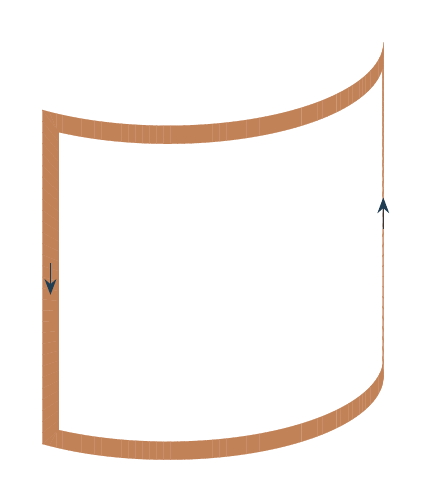
\begin{tikzpicture}[x=6.22317cm,y=6.22317cm]
\path[use as bounding box] (-0.378154,-0.455828) rectangle (0.378154,0.455828);
\path[fill=copper!82,draw=copper!82,line width=.08pt] (-0.086270,0.255757) -- (-0.100668,0.255778) -- (-0.100668,0.218935) -- (-0.086270,0.218914) -- cycle;
\path[fill=copper!82,draw=copper!82,line width=.08pt] (-0.071877,0.255920) -- (-0.086270,0.255757) -- (-0.086270,0.218914) -- (-0.071877,0.219077) -- cycle;
\path[fill=copper!82,draw=copper!82,line width=.08pt] (-0.100668,0.255778) -- (-0.115057,0.255982) -- (-0.115057,0.219140) -- (-0.100668,0.218935) -- cycle;
\path[fill=copper!82,draw=copper!82,line width=.08pt] (-0.057506,0.256265) -- (-0.071877,0.255920) -- (-0.071877,0.219077) -- (-0.057506,0.219423) -- cycle;
\path[fill=copper!82,draw=copper!82,line width=.08pt] (-0.115057,0.255982) -- (-0.129420,0.256369) -- (-0.129420,0.219527) -- (-0.115057,0.219140) -- cycle;
\path[fill=copper!82,draw=copper!82,line width=.08pt] (-0.043172,0.256794) -- (-0.057506,0.256265) -- (-0.057506,0.219423) -- (-0.043172,0.219952) -- cycle;
\path[fill=copper!82,draw=copper!82,line width=.08pt] (-0.129420,0.256369) -- (-0.143744,0.256940) -- (-0.143744,0.220097) -- (-0.129420,0.219527) -- cycle;
\path[fill=copper!82,draw=copper!82,line width=.08pt] (-0.028890,0.257505) -- (-0.043172,0.256794) -- (-0.043172,0.219952) -- (-0.028890,0.220663) -- cycle;
\path[fill=copper!82,draw=copper!82,line width=.08pt] (-0.143744,0.256940) -- (-0.158012,0.257692) -- (-0.158012,0.220850) -- (-0.143744,0.220097) -- cycle;
\path[fill=copper!82,draw=copper!82,line width=.08pt] (-0.014676,0.258398) -- (-0.028890,0.257505) -- (-0.028890,0.220663) -- (-0.014676,0.221556) -- cycle;
\path[fill=copper!82,draw=copper!82,line width=.08pt] (-0.158012,0.257692) -- (-0.172209,0.258626) -- (-0.172209,0.221784) -- (-0.158012,0.220850) -- cycle;
\path[fill=copper!82,draw=copper!82,line width=.08pt] (-0.000544,0.259472) -- (-0.014676,0.258398) -- (-0.014676,0.221556) -- (-0.000544,0.222629) -- cycle;
\path[fill=copper!82,draw=copper!82,line width=.08pt] (-0.172209,0.258626) -- (-0.186320,0.259740) -- (-0.186320,0.222898) -- (-0.172209,0.221784) -- cycle;
\path[fill=copper!82,draw=copper!82,line width=.08pt] (0.013491,0.260725) -- (-0.000544,0.259472) -- (-0.000544,0.222629) -- (0.013491,0.223882) -- cycle;
\path[fill=copper!82,draw=copper!82,line width=.08pt] (-0.186320,0.259740) -- (-0.200330,0.261034) -- (-0.200330,0.224192) -- (-0.186320,0.222898) -- cycle;
\path[fill=copper!82,draw=copper!82,line width=.08pt] (0.027412,0.262156) -- (0.013491,0.260725) -- (0.013491,0.223882) -- (0.027412,0.225313) -- cycle;
\path[fill=copper!82,draw=copper!82,line width=.08pt] (-0.200330,0.261034) -- (-0.214224,0.262505) -- (-0.214224,0.225663) -- (-0.200330,0.224192) -- cycle;
\path[fill=copper!82,draw=copper!82,line width=.08pt] (0.041206,0.263763) -- (0.027412,0.262156) -- (0.027412,0.225313) -- (0.041206,0.226921) -- cycle;
\path[fill=copper!82,draw=copper!82,line width=.08pt] (-0.214224,0.262505) -- (-0.227987,0.264153) -- (-0.227987,0.227310) -- (-0.214224,0.225663) -- cycle;
\path[fill=copper!82,draw=copper!82,line width=.08pt] (0.054857,0.265546) -- (0.041206,0.263763) -- (0.041206,0.226921) -- (0.054857,0.228703) -- cycle;
\path[fill=copper!82,draw=copper!82,line width=.08pt] (-0.227987,0.264153) -- (-0.241604,0.265975) -- (-0.241604,0.229132) -- (-0.227987,0.227310) -- cycle;
\path[fill=copper!82,draw=copper!82,line width=.08pt] (0.068351,0.267501) -- (0.054857,0.265546) -- (0.054857,0.228703) -- (0.068351,0.230659) -- cycle;
\path[fill=copper!82,draw=copper!82,line width=.08pt] (-0.241604,0.265975) -- (-0.255060,0.267969) -- (-0.255060,0.231127) -- (-0.241604,0.229132) -- cycle;
\path[fill=copper!82,draw=copper!82,line width=.08pt] (0.081674,0.269628) -- (0.068351,0.267501) -- (0.068351,0.230659) -- (0.081674,0.232785) -- cycle;
\path[fill=copper!82,draw=copper!82,line width=.08pt] (-0.255060,0.267969) -- (-0.268342,0.270134) -- (-0.268342,0.233292) -- (-0.255060,0.231127) -- cycle;
\path[fill=copper!82,draw=copper!82,line width=.08pt] (0.094811,0.271923) -- (0.081674,0.269628) -- (0.081674,0.232785) -- (0.094811,0.235081) -- cycle;
\path[fill=copper!82,draw=copper!82,line width=.08pt] (-0.268342,0.270134) -- (-0.281435,0.272467) -- (-0.281435,0.235625) -- (-0.268342,0.233292) -- cycle;
\path[fill=copper!82,draw=copper!82,line width=.08pt] (0.107748,0.274384) -- (0.094811,0.271923) -- (0.094811,0.235081) -- (0.107748,0.237542) -- cycle;
\path[fill=copper!82,draw=copper!82,line width=.08pt] (-0.281435,0.272467) -- (-0.294325,0.274966) -- (-0.294325,0.238123) -- (-0.281435,0.235625) -- cycle;
\path[fill=copper!82,draw=copper!82,line width=.08pt] (0.120471,0.277009) -- (0.107748,0.274384) -- (0.107748,0.237542) -- (0.120471,0.240166) -- cycle;
\path[fill=copper!82,draw=copper!82,line width=.08pt] (-0.294325,0.274966) -- (-0.306997,0.277627) -- (-0.306997,0.240785) -- (-0.294325,0.238123) -- cycle;
\path[fill=copper!82,draw=copper!82,line width=.08pt] (0.132967,0.279794) -- (0.120471,0.277009) -- (0.120471,0.240166) -- (0.132967,0.242952) -- cycle;
\path[fill=copper!82,draw=copper!82,line width=.08pt] (-0.306997,0.277627) -- (-0.319440,0.280449) -- (-0.319440,0.243606) -- (-0.306997,0.240785) -- cycle;
\path[fill=copper!82,draw=copper!82,line width=.08pt] (-0.319440,0.280449) -- (-0.333982,0.284025) -- (-0.317039,0.243045) -- (-0.319440,0.243606) -- cycle;
\path[fill=copper!82,draw=copper!82,line width=.08pt] (0.145223,0.282737) -- (0.132967,0.279794) -- (0.132967,0.242952) -- (0.145223,0.245895) -- cycle;
\path[fill=copper!82,draw=copper!82,line width=.08pt] (-0.333982,0.284025) -- (-0.348154,0.287819) -- (-0.314628,0.242490) -- (-0.317039,0.243045) -- cycle;
\path[fill=copper!82,draw=copper!82,line width=.08pt] (0.157224,0.285835) -- (0.145223,0.282737) -- (0.145223,0.245895) -- (0.157224,0.248993) -- cycle;
\path[fill=copper!82,draw=copper!82,line width=.08pt] (-0.348154,0.287819) -- (-0.348154,0.265099) -- (-0.314628,0.222227) -- (-0.314628,0.242490) -- cycle;
\path[fill=copper!82,draw=copper!82,line width=.08pt] (0.168959,0.289084) -- (0.157224,0.285835) -- (0.157224,0.248993) -- (0.168959,0.252242) -- cycle;
\path[fill=copper!82,draw=copper!82,line width=.08pt] (-0.348154,0.265099) -- (-0.348154,0.242380) -- (-0.314628,0.201963) -- (-0.314628,0.222227) -- cycle;
\path[fill=copper!82,draw=copper!82,line width=.08pt] (0.180414,0.292481) -- (0.168959,0.289084) -- (0.168959,0.252242) -- (0.180414,0.255638) -- cycle;
\path[fill=copper!82,draw=copper!82,line width=.08pt] (-0.348154,0.242380) -- (-0.348154,0.219660) -- (-0.314628,0.181700) -- (-0.314628,0.201963) -- cycle;
\path[fill=copper!82,draw=copper!82,line width=.08pt] (0.191578,0.296022) -- (0.180414,0.292481) -- (0.180414,0.255638) -- (0.191578,0.259179) -- cycle;
\path[fill=copper!82,draw=copper!82,line width=.08pt] (-0.348154,0.219660) -- (-0.348154,0.196941) -- (-0.314628,0.161437) -- (-0.314628,0.181700) -- cycle;
\path[fill=copper!82,draw=copper!82,line width=.08pt] (0.202438,0.299703) -- (0.191578,0.296022) -- (0.191578,0.259179) -- (0.202438,0.262861) -- cycle;
\path[fill=copper!82,draw=copper!82,line width=.08pt] (-0.348154,0.196941) -- (-0.348154,0.174221) -- (-0.314628,0.141173) -- (-0.314628,0.161437) -- cycle;
\path[fill=copper!82,draw=copper!82,line width=.08pt] (0.212984,0.303521) -- (0.202438,0.299703) -- (0.202438,0.262861) -- (0.212984,0.266678) -- cycle;
\path[fill=copper!82,draw=copper!82,line width=.08pt] (-0.348154,0.174221) -- (-0.348154,0.151502) -- (-0.314628,0.120910) -- (-0.314628,0.141173) -- cycle;
\path[fill=copper!82,draw=copper!82,line width=.08pt] (0.223203,0.307471) -- (0.212984,0.303521) -- (0.212984,0.266678) -- (0.223203,0.270628) -- cycle;
\path[fill=copper!82,draw=copper!82,line width=.08pt] (-0.348154,0.151502) -- (-0.348154,0.128782) -- (-0.314628,0.100647) -- (-0.314628,0.120910) -- cycle;
\path[fill=copper!82,draw=copper!82,line width=.08pt] (0.233084,0.311549) -- (0.223203,0.307471) -- (0.223203,0.270628) -- (0.233084,0.274706) -- cycle;
\path[fill=copper!82,draw=copper!82,line width=.08pt] (-0.348154,0.128782) -- (-0.348154,0.106063) -- (-0.314628,0.080383) -- (-0.314628,0.100647) -- cycle;
\path[fill=copper!82,draw=copper!82,line width=.08pt] (0.242618,0.315751) -- (0.233084,0.311549) -- (0.233084,0.274706) -- (0.242618,0.278908) -- cycle;
\path[fill=copper!82,draw=copper!82,line width=.08pt] (-0.348154,0.106063) -- (-0.348154,0.083343) -- (-0.314628,0.060120) -- (-0.314628,0.080383) -- cycle;
\path[fill=copper!82,draw=copper!82,line width=.08pt] (0.251793,0.320072) -- (0.242618,0.315751) -- (0.242618,0.278908) -- (0.251793,0.283229) -- cycle;
\path[fill=copper!82,draw=copper!82,line width=.08pt] (-0.348154,0.083343) -- (-0.348154,0.060624) -- (-0.314628,0.039857) -- (-0.314628,0.060120) -- cycle;
\path[fill=copper!82,draw=copper!82,line width=.08pt] (0.260601,0.324507) -- (0.251793,0.320072) -- (0.251793,0.283229) -- (0.260601,0.287665) -- cycle;
\path[fill=copper!82,draw=copper!82,line width=.08pt] (-0.348154,0.060624) -- (-0.348154,0.037904) -- (-0.314628,0.019593) -- (-0.314628,0.039857) -- cycle;
\path[fill=copper!82,draw=copper!82,line width=.08pt] (0.269031,0.329053) -- (0.260601,0.324507) -- (0.260601,0.287665) -- (0.269031,0.292210) -- cycle;
\path[fill=copper!82,draw=copper!82,line width=.08pt] (-0.348154,0.037904) -- (-0.348154,0.015185) -- (-0.314628,-0.000670) -- (-0.314628,0.019593) -- cycle;
\path[fill=copper!82,draw=copper!82,line width=.08pt] (0.277075,0.333703) -- (0.269031,0.329053) -- (0.269031,0.292210) -- (0.277075,0.296861) -- cycle;
\path[fill=copper!82,draw=copper!82,line width=.08pt] (-0.348154,0.015185) -- (-0.348154,-0.007535) -- (-0.314628,-0.020933) -- (-0.314628,-0.000670) -- cycle;
\path[fill=copper!82,draw=copper!82,line width=.08pt] (-0.348154,-0.007535) -- (-0.348154,-0.030254) -- (-0.314628,-0.041197) -- (-0.314628,-0.020933) -- cycle;
\path[fill=copper!82,draw=copper!82,line width=.08pt] (0.284723,0.338453) -- (0.277075,0.333703) -- (0.277075,0.296861) -- (0.284723,0.301611) -- cycle;
\path[fill=copper!82,draw=copper!82,line width=.08pt] (-0.348154,-0.030254) -- (-0.348154,-0.052974) -- (-0.314628,-0.061460) -- (-0.314628,-0.041197) -- cycle;
\path[fill=copper!82,draw=copper!82,line width=.08pt] (0.291969,0.343299) -- (0.284723,0.338453) -- (0.284723,0.301611) -- (0.291969,0.306456) -- cycle;
\path[fill=copper!82,draw=copper!82,line width=.08pt] (-0.348154,-0.052974) -- (-0.348154,-0.075693) -- (-0.314628,-0.081723) -- (-0.314628,-0.061460) -- cycle;
\path[fill=copper!82,draw=copper!82,line width=.08pt] (0.298803,0.348234) -- (0.291969,0.343299) -- (0.291969,0.306456) -- (0.298803,0.311391) -- cycle;
\path[fill=copper!82,draw=copper!82,line width=.08pt] (-0.348154,-0.075693) -- (-0.348154,-0.098413) -- (-0.314628,-0.101987) -- (-0.314628,-0.081723) -- cycle;
\path[fill=copper!82,draw=copper!82,line width=.08pt] (0.305219,0.353253) -- (0.298803,0.348234) -- (0.298803,0.311391) -- (0.305219,0.316411) -- cycle;
\path[fill=copper!82,draw=copper!82,line width=.08pt] (-0.348154,-0.098413) -- (-0.348154,-0.121132) -- (-0.314628,-0.122250) -- (-0.314628,-0.101987) -- cycle;
\path[fill=copper!82,draw=copper!82,line width=.08pt] (-0.348154,-0.121132) -- (-0.348154,-0.143852) -- (-0.314628,-0.142513) -- (-0.314628,-0.122250) -- cycle;
\path[fill=copper!82,draw=copper!82,line width=.08pt] (0.311210,0.358352) -- (0.305219,0.353253) -- (0.305219,0.316411) -- (0.311210,0.321509) -- cycle;
\path[fill=copper!82,draw=copper!82,line width=.08pt] (-0.348154,-0.143852) -- (-0.348154,-0.166571) -- (-0.314628,-0.162777) -- (-0.314628,-0.142513) -- cycle;
\path[fill=copper!82,draw=copper!82,line width=.08pt] (0.316770,0.363524) -- (0.311210,0.358352) -- (0.311210,0.321509) -- (0.316770,0.326682) -- cycle;
\path[fill=copper!82,draw=copper!82,line width=.08pt] (-0.348154,-0.166571) -- (-0.348154,-0.189291) -- (-0.314628,-0.183040) -- (-0.314628,-0.162777) -- cycle;
\path[fill=copper!82,draw=copper!82,line width=.08pt] (0.321892,0.368764) -- (0.316770,0.363524) -- (0.316770,0.326682) -- (0.321892,0.331922) -- cycle;
\path[fill=copper!82,draw=copper!82,line width=.08pt] (-0.348154,-0.189291) -- (-0.348154,-0.212010) -- (-0.314628,-0.203304) -- (-0.314628,-0.183040) -- cycle;
\path[fill=copper!82,draw=copper!82,line width=.08pt] (-0.348154,-0.212010) -- (-0.348154,-0.234730) -- (-0.314628,-0.223567) -- (-0.314628,-0.203304) -- cycle;
\path[fill=copper!82,draw=copper!82,line width=.08pt] (-0.100668,-0.425807) -- (-0.086270,-0.425828) -- (-0.086270,-0.388986) -- (-0.100668,-0.388965) -- cycle;
\path[fill=copper!82,draw=copper!82,line width=.08pt] (-0.086270,-0.425828) -- (-0.071877,-0.425666) -- (-0.071877,-0.388823) -- (-0.086270,-0.388986) -- cycle;
\path[fill=copper!82,draw=copper!82,line width=.08pt] (-0.115057,-0.425603) -- (-0.100668,-0.425807) -- (-0.100668,-0.388965) -- (-0.115057,-0.388761) -- cycle;
\path[fill=copper!82,draw=copper!82,line width=.08pt] (-0.071877,-0.425666) -- (-0.057506,-0.425320) -- (-0.057506,-0.388477) -- (-0.071877,-0.388823) -- cycle;
\path[fill=copper!82,draw=copper!82,line width=.08pt] (0.326570,0.374067) -- (0.321892,0.368764) -- (0.321892,0.331922) -- (0.326570,0.337224) -- cycle;
\path[fill=copper!82,draw=copper!82,line width=.08pt] (-0.129420,-0.425216) -- (-0.115057,-0.425603) -- (-0.115057,-0.388761) -- (-0.129420,-0.388373) -- cycle;
\path[fill=copper!82,draw=copper!82,line width=.08pt] (-0.057506,-0.425320) -- (-0.043172,-0.424791) -- (-0.043172,-0.387948) -- (-0.057506,-0.388477) -- cycle;
\path[fill=copper!82,draw=copper!82,line width=.08pt] (-0.143744,-0.424645) -- (-0.129420,-0.425216) -- (-0.129420,-0.388373) -- (-0.143744,-0.387803) -- cycle;
\path[fill=copper!82,draw=copper!82,line width=.08pt] (-0.043172,-0.424791) -- (-0.028890,-0.424080) -- (-0.028890,-0.387237) -- (-0.043172,-0.387948) -- cycle;
\path[fill=copper!82,draw=copper!82,line width=.08pt] (-0.158012,-0.423893) -- (-0.143744,-0.424645) -- (-0.143744,-0.387803) -- (-0.158012,-0.387050) -- cycle;
\path[fill=copper!82,draw=copper!82,line width=.08pt] (-0.028890,-0.424080) -- (-0.014676,-0.423187) -- (-0.014676,-0.386344) -- (-0.028890,-0.387237) -- cycle;
\path[fill=copper!82,draw=copper!82,line width=.08pt] (-0.172209,-0.422959) -- (-0.158012,-0.423893) -- (-0.158012,-0.387050) -- (-0.172209,-0.386117) -- cycle;
\path[fill=copper!82,draw=copper!82,line width=.08pt] (-0.348154,-0.234730) -- (-0.348154,-0.257449) -- (-0.314628,-0.243830) -- (-0.314628,-0.223567) -- cycle;
\path[fill=copper!82,draw=copper!82,line width=.08pt] (-0.014676,-0.423187) -- (-0.000544,-0.422113) -- (-0.000544,-0.385271) -- (-0.014676,-0.386344) -- cycle;
\path[fill=copper!82,draw=copper!82,line width=.08pt] (-0.186320,-0.421845) -- (-0.172209,-0.422959) -- (-0.172209,-0.386117) -- (-0.186320,-0.385002) -- cycle;
\path[fill=copper!82,draw=copper!82,line width=.08pt] (-0.000544,-0.422113) -- (0.013491,-0.420861) -- (0.013491,-0.384018) -- (-0.000544,-0.385271) -- cycle;
\path[fill=copper!82,draw=copper!82,line width=.08pt] (-0.200330,-0.420551) -- (-0.186320,-0.421845) -- (-0.186320,-0.385002) -- (-0.200330,-0.383709) -- cycle;
\path[fill=copper!82,draw=copper!82,line width=.08pt] (0.013491,-0.420861) -- (0.027412,-0.419429) -- (0.027412,-0.382587) -- (0.013491,-0.384018) -- cycle;
\path[fill=copper!82,draw=copper!82,line width=.08pt] (0.330801,0.379426) -- (0.326570,0.374067) -- (0.326570,0.337224) -- (0.330801,0.342584) -- cycle;
\path[fill=copper!82,draw=copper!82,line width=.08pt] (-0.214224,-0.419080) -- (-0.200330,-0.420551) -- (-0.200330,-0.383709) -- (-0.214224,-0.382237) -- cycle;
\path[fill=copper!82,draw=copper!82,line width=.08pt] (-0.348154,-0.257449) -- (-0.348154,-0.280169) -- (-0.314628,-0.264094) -- (-0.314628,-0.243830) -- cycle;
\path[fill=copper!82,draw=copper!82,line width=.08pt] (0.027412,-0.419429) -- (0.041206,-0.417822) -- (0.041206,-0.380979) -- (0.027412,-0.382587) -- cycle;
\path[fill=copper!82,draw=copper!82,line width=.08pt] (-0.227987,-0.417432) -- (-0.214224,-0.419080) -- (-0.214224,-0.382237) -- (-0.227987,-0.380590) -- cycle;
\path[fill=copper!82,draw=copper!82,line width=.08pt] (0.041206,-0.417822) -- (0.054857,-0.416039) -- (0.054857,-0.379197) -- (0.041206,-0.380979) -- cycle;
\path[fill=copper!82,draw=copper!82,line width=.08pt] (-0.241604,-0.415610) -- (-0.227987,-0.417432) -- (-0.227987,-0.380590) -- (-0.241604,-0.378768) -- cycle;
\path[fill=copper!82,draw=copper!82,line width=.08pt] (-0.348154,-0.280169) -- (-0.348154,-0.302888) -- (-0.314628,-0.284357) -- (-0.314628,-0.264094) -- cycle;
\path[fill=copper!82,draw=copper!82,line width=.08pt] (0.054857,-0.416039) -- (0.068351,-0.414084) -- (0.068351,-0.377241) -- (0.054857,-0.379197) -- cycle;
\path[fill=copper!82,draw=copper!82,line width=.08pt] (0.334579,0.384837) -- (0.330801,0.379426) -- (0.330801,0.342584) -- (0.334579,0.347994) -- cycle;
\path[fill=copper!82,draw=copper!82,line width=.08pt] (-0.255060,-0.413616) -- (-0.241604,-0.415610) -- (-0.241604,-0.378768) -- (-0.255060,-0.376773) -- cycle;
\path[fill=copper!82,draw=copper!82,line width=.08pt] (0.068351,-0.414084) -- (0.081674,-0.411957) -- (0.081674,-0.375115) -- (0.068351,-0.377241) -- cycle;
\path[fill=copper!82,draw=copper!82,line width=.08pt] (-0.268342,-0.411451) -- (-0.255060,-0.413616) -- (-0.255060,-0.376773) -- (-0.268342,-0.374608) -- cycle;
\path[fill=copper!82,draw=copper!82,line width=.08pt] (-0.348154,-0.302888) -- (-0.348154,-0.325608) -- (-0.314628,-0.304620) -- (-0.314628,-0.284357) -- cycle;
\path[fill=copper!82,draw=copper!82,line width=.08pt] (0.081674,-0.411957) -- (0.094811,-0.409662) -- (0.094811,-0.372820) -- (0.081674,-0.375115) -- cycle;
\path[fill=copper!82,draw=copper!82,line width=.08pt] (-0.281435,-0.409118) -- (-0.268342,-0.411451) -- (-0.268342,-0.374608) -- (-0.281435,-0.372275) -- cycle;
\path[fill=copper!82,draw=copper!82,line width=.08pt] (0.337901,0.390293) -- (0.334579,0.384837) -- (0.334579,0.347994) -- (0.337901,0.353450) -- cycle;
\path[fill=copper!82,draw=copper!82,line width=.08pt] (0.094811,-0.409662) -- (0.107748,-0.407201) -- (0.107748,-0.370359) -- (0.094811,-0.372820) -- cycle;
\path[fill=copper!82,draw=copper!82,line width=.08pt] (-0.294325,-0.406619) -- (-0.281435,-0.409118) -- (-0.281435,-0.372275) -- (-0.294325,-0.369777) -- cycle;
\path[fill=copper!82,draw=copper!82,line width=.08pt] (-0.348154,-0.325608) -- (-0.348154,-0.348327) -- (-0.314628,-0.324884) -- (-0.314628,-0.304620) -- cycle;
\path[fill=copper!82,draw=copper!82,line width=.08pt] (0.107748,-0.407201) -- (0.120471,-0.404576) -- (0.120471,-0.367734) -- (0.107748,-0.370359) -- cycle;
\path[fill=copper!82,draw=copper!82,line width=.08pt] (-0.306997,-0.403958) -- (-0.294325,-0.406619) -- (-0.294325,-0.369777) -- (-0.306997,-0.367115) -- cycle;
\path[fill=copper!82,draw=copper!82,line width=.08pt] (0.340762,0.395788) -- (0.337901,0.390293) -- (0.337901,0.353450) -- (0.340762,0.358945) -- cycle;
\path[fill=copper!82,draw=copper!82,line width=.08pt] (-0.348154,-0.348327) -- (-0.348154,-0.371047) -- (-0.314628,-0.345147) -- (-0.314628,-0.324884) -- cycle;
\path[fill=copper!82,draw=copper!82,line width=.08pt] (0.120471,-0.404576) -- (0.132967,-0.401791) -- (0.132967,-0.364948) -- (0.120471,-0.367734) -- cycle;
\path[fill=copper!82,draw=copper!82,line width=.08pt] (-0.319440,-0.401136) -- (-0.306997,-0.403958) -- (-0.306997,-0.367115) -- (-0.319440,-0.364294) -- cycle;
\path[fill=copper!82,draw=copper!82,line width=.08pt] (-0.333982,-0.397561) -- (-0.319440,-0.401136) -- (-0.319440,-0.364294) -- (-0.317039,-0.364855) -- cycle;
\path[fill=copper!82,draw=copper!82,line width=.08pt] (0.132967,-0.401791) -- (0.145223,-0.398848) -- (0.145223,-0.362005) -- (0.132967,-0.364948) -- cycle;
\path[fill=copper!82,draw=copper!82,line width=.08pt] (-0.348154,-0.371047) -- (-0.348154,-0.393766) -- (-0.314628,-0.365410) -- (-0.314628,-0.345147) -- cycle;
\path[fill=copper!82,draw=copper!82,line width=.08pt] (-0.348154,-0.393766) -- (-0.333982,-0.397561) -- (-0.317039,-0.364855) -- (-0.314628,-0.365410) -- cycle;
\path[fill=copper!82,draw=copper!82,line width=.08pt] (0.343161,0.401316) -- (0.340762,0.395788) -- (0.340762,0.358945) -- (0.343161,0.364474) -- cycle;
\path[fill=copper!82,draw=copper!82,line width=.08pt] (0.145223,-0.398848) -- (0.157224,-0.395750) -- (0.157224,-0.358908) -- (0.145223,-0.362005) -- cycle;
\path[fill=copper!82,draw=copper!82,line width=.08pt] (0.157224,-0.395750) -- (0.168959,-0.392501) -- (0.168959,-0.355659) -- (0.157224,-0.358908) -- cycle;
\path[fill=copper!82,draw=copper!82,line width=.08pt] (0.345093,0.406873) -- (0.343161,0.401316) -- (0.343161,0.364474) -- (0.345093,0.370030) -- cycle;
\path[fill=copper!82,draw=copper!82,line width=.08pt] (0.168959,-0.392501) -- (0.180414,-0.389104) -- (0.180414,-0.352262) -- (0.168959,-0.355659) -- cycle;
\path[fill=copper!82,draw=copper!82,line width=.08pt] (0.180414,-0.389104) -- (0.191578,-0.385563) -- (0.191578,-0.348721) -- (0.180414,-0.352262) -- cycle;
\path[fill=copper!82,draw=copper!82,line width=.08pt] (0.346557,0.412451) -- (0.345093,0.406873) -- (0.345093,0.370030) -- (0.346557,0.375608) -- cycle;
\path[fill=copper!82,draw=copper!82,line width=.08pt] (0.191578,-0.385563) -- (0.202438,-0.381882) -- (0.202438,-0.345040) -- (0.191578,-0.348721) -- cycle;
\path[fill=copper!82,draw=copper!82,line width=.08pt] (0.347691,0.419133) -- (0.346557,0.412451) -- (0.346557,0.375608) -- (0.346309,0.374522) -- cycle;
\path[fill=copper!82,draw=copper!82,line width=.08pt] (0.348154,0.425828) -- (0.347691,0.419133) -- (0.346309,0.374522) -- (0.346043,0.373436) -- cycle;
\path[fill=copper!82,draw=copper!82,line width=.08pt] (0.202438,-0.381882) -- (0.212984,-0.378064) -- (0.212984,-0.341222) -- (0.202438,-0.345040) -- cycle;
\path[fill=copper!82,draw=copper!82,line width=.08pt] (0.348154,0.403109) -- (0.348154,0.425828) -- (0.346043,0.373436) -- (0.346043,0.353173) -- cycle;
\path[fill=copper!82,draw=copper!82,line width=.08pt] (0.212984,-0.378064) -- (0.223203,-0.374114) -- (0.223203,-0.337272) -- (0.212984,-0.341222) -- cycle;
\path[fill=copper!82,draw=copper!82,line width=.08pt] (0.348154,0.380389) -- (0.348154,0.403109) -- (0.346043,0.353173) -- (0.346043,0.332909) -- cycle;
\path[fill=copper!82,draw=copper!82,line width=.08pt] (0.223203,-0.374114) -- (0.233084,-0.370036) -- (0.233084,-0.333194) -- (0.223203,-0.337272) -- cycle;
\path[fill=copper!82,draw=copper!82,line width=.08pt] (0.348154,0.357670) -- (0.348154,0.380389) -- (0.346043,0.332909) -- (0.346043,0.312646) -- cycle;
\path[fill=copper!82,draw=copper!82,line width=.08pt] (0.233084,-0.370036) -- (0.242618,-0.365835) -- (0.242618,-0.328992) -- (0.233084,-0.333194) -- cycle;
\path[fill=copper!82,draw=copper!82,line width=.08pt] (0.348154,0.334950) -- (0.348154,0.357670) -- (0.346043,0.312646) -- (0.346043,0.292383) -- cycle;
\path[fill=copper!82,draw=copper!82,line width=.08pt] (0.242618,-0.365835) -- (0.251793,-0.361514) -- (0.251793,-0.324671) -- (0.242618,-0.328992) -- cycle;
\path[fill=copper!82,draw=copper!82,line width=.08pt] (0.348154,0.312231) -- (0.348154,0.334950) -- (0.346043,0.292383) -- (0.346043,0.272119) -- cycle;
\path[fill=copper!82,draw=copper!82,line width=.08pt] (0.251793,-0.361514) -- (0.260601,-0.357078) -- (0.260601,-0.320236) -- (0.251793,-0.324671) -- cycle;
\path[fill=copper!82,draw=copper!82,line width=.08pt] (0.348154,0.289511) -- (0.348154,0.312231) -- (0.346043,0.272119) -- (0.346043,0.251856) -- cycle;
\path[fill=copper!82,draw=copper!82,line width=.08pt] (0.260601,-0.357078) -- (0.269031,-0.352533) -- (0.269031,-0.315690) -- (0.260601,-0.320236) -- cycle;
\path[fill=copper!82,draw=copper!82,line width=.08pt] (0.348154,0.266792) -- (0.348154,0.289511) -- (0.346043,0.251856) -- (0.346043,0.231593) -- cycle;
\path[fill=copper!82,draw=copper!82,line width=.08pt] (0.269031,-0.352533) -- (0.277075,-0.347882) -- (0.277075,-0.311040) -- (0.269031,-0.315690) -- cycle;
\path[fill=copper!82,draw=copper!82,line width=.08pt] (0.348154,0.244072) -- (0.348154,0.266792) -- (0.346043,0.231593) -- (0.346043,0.211329) -- cycle;
\path[fill=copper!82,draw=copper!82,line width=.08pt] (0.348154,0.221353) -- (0.348154,0.244072) -- (0.346043,0.211329) -- (0.346043,0.191066) -- cycle;
\path[fill=copper!82,draw=copper!82,line width=.08pt] (0.277075,-0.347882) -- (0.284723,-0.343132) -- (0.284723,-0.306289) -- (0.277075,-0.311040) -- cycle;
\path[fill=copper!82,draw=copper!82,line width=.08pt] (0.348154,0.198633) -- (0.348154,0.221353) -- (0.346043,0.191066) -- (0.346043,0.170803) -- cycle;
\path[fill=copper!82,draw=copper!82,line width=.08pt] (0.284723,-0.343132) -- (0.291969,-0.338286) -- (0.291969,-0.301444) -- (0.284723,-0.306289) -- cycle;
\path[fill=copper!82,draw=copper!82,line width=.08pt] (0.348154,0.175914) -- (0.348154,0.198633) -- (0.346043,0.170803) -- (0.346043,0.150539) -- cycle;
\path[fill=copper!82,draw=copper!82,line width=.08pt] (0.291969,-0.338286) -- (0.298803,-0.333351) -- (0.298803,-0.296509) -- (0.291969,-0.301444) -- cycle;
\path[fill=copper!82,draw=copper!82,line width=.08pt] (0.348154,0.153194) -- (0.348154,0.175914) -- (0.346043,0.150539) -- (0.346043,0.130276) -- cycle;
\path[fill=copper!82,draw=copper!82,line width=.08pt] (0.298803,-0.333351) -- (0.305219,-0.328332) -- (0.305219,-0.291489) -- (0.298803,-0.296509) -- cycle;
\path[fill=copper!82,draw=copper!82,line width=.08pt] (0.348154,0.130475) -- (0.348154,0.153194) -- (0.346043,0.130276) -- (0.346043,0.110013) -- cycle;
\path[fill=copper!82,draw=copper!82,line width=.08pt] (0.348154,0.107755) -- (0.348154,0.130475) -- (0.346043,0.110013) -- (0.346043,0.089749) -- cycle;
\path[fill=copper!82,draw=copper!82,line width=.08pt] (0.305219,-0.328332) -- (0.311210,-0.323233) -- (0.311210,-0.286391) -- (0.305219,-0.291489) -- cycle;
\path[fill=copper!82,draw=copper!82,line width=.08pt] (0.348154,0.085036) -- (0.348154,0.107755) -- (0.346043,0.089749) -- (0.346043,0.069486) -- cycle;
\path[fill=copper!82,draw=copper!82,line width=.08pt] (0.311210,-0.323233) -- (0.316770,-0.318061) -- (0.316770,-0.281219) -- (0.311210,-0.286391) -- cycle;
\path[fill=copper!82,draw=copper!82,line width=.08pt] (0.348154,0.062316) -- (0.348154,0.085036) -- (0.346043,0.069486) -- (0.346043,0.049223) -- cycle;
\path[fill=copper!82,draw=copper!82,line width=.08pt] (0.316770,-0.318061) -- (0.321892,-0.312821) -- (0.321892,-0.275978) -- (0.316770,-0.281219) -- cycle;
\path[fill=copper!82,draw=copper!82,line width=.08pt] (0.348154,0.039597) -- (0.348154,0.062316) -- (0.346043,0.049223) -- (0.346043,0.028959) -- cycle;
\path[fill=copper!82,draw=copper!82,line width=.08pt] (0.348154,0.016877) -- (0.348154,0.039597) -- (0.346043,0.028959) -- (0.346043,0.008696) -- cycle;
\path[fill=copper!82,draw=copper!82,line width=.08pt] (0.321892,-0.312821) -- (0.326570,-0.307518) -- (0.326570,-0.270676) -- (0.321892,-0.275978) -- cycle;
\path[fill=copper!82,draw=copper!82,line width=.08pt] (0.348154,-0.005842) -- (0.348154,0.016877) -- (0.346043,0.008696) -- (0.346043,-0.011567) -- cycle;
\path[fill=copper!82,draw=copper!82,line width=.08pt] (0.326570,-0.307518) -- (0.330801,-0.302159) -- (0.330801,-0.265316) -- (0.326570,-0.270676) -- cycle;
\path[fill=copper!82,draw=copper!82,line width=.08pt] (0.348154,-0.028562) -- (0.348154,-0.005842) -- (0.346043,-0.011567) -- (0.346043,-0.031831) -- cycle;
\path[fill=copper!82,draw=copper!82,line width=.08pt] (0.348154,-0.051281) -- (0.348154,-0.028562) -- (0.346043,-0.031831) -- (0.346043,-0.052094) -- cycle;
\path[fill=copper!82,draw=copper!82,line width=.08pt] (0.330801,-0.302159) -- (0.334579,-0.296748) -- (0.334579,-0.259906) -- (0.330801,-0.265316) -- cycle;
\path[fill=copper!82,draw=copper!82,line width=.08pt] (0.348154,-0.074001) -- (0.348154,-0.051281) -- (0.346043,-0.052094) -- (0.346043,-0.072357) -- cycle;
\path[fill=copper!82,draw=copper!82,line width=.08pt] (0.334579,-0.296748) -- (0.337901,-0.291293) -- (0.337901,-0.254450) -- (0.334579,-0.259906) -- cycle;
\path[fill=copper!82,draw=copper!82,line width=.08pt] (0.348154,-0.096720) -- (0.348154,-0.074001) -- (0.346043,-0.072357) -- (0.346043,-0.092621) -- cycle;
\path[fill=copper!82,draw=copper!82,line width=.08pt] (0.337901,-0.291293) -- (0.340762,-0.285797) -- (0.340762,-0.248955) -- (0.337901,-0.254450) -- cycle;
\path[fill=copper!82,draw=copper!82,line width=.08pt] (0.348154,-0.119440) -- (0.348154,-0.096720) -- (0.346043,-0.092621) -- (0.346043,-0.112884) -- cycle;
\path[fill=copper!82,draw=copper!82,line width=.08pt] (0.348154,-0.142159) -- (0.348154,-0.119440) -- (0.346043,-0.112884) -- (0.346043,-0.133147) -- cycle;
\path[fill=copper!82,draw=copper!82,line width=.08pt] (0.340762,-0.285797) -- (0.343161,-0.280269) -- (0.343161,-0.243426) -- (0.340762,-0.248955) -- cycle;
\path[fill=copper!82,draw=copper!82,line width=.08pt] (0.348154,-0.164879) -- (0.348154,-0.142159) -- (0.346043,-0.133147) -- (0.346043,-0.153411) -- cycle;
\path[fill=copper!82,draw=copper!82,line width=.08pt] (0.343161,-0.280269) -- (0.345093,-0.274713) -- (0.345093,-0.237870) -- (0.343161,-0.243426) -- cycle;
\path[fill=copper!82,draw=copper!82,line width=.08pt] (0.348154,-0.187598) -- (0.348154,-0.164879) -- (0.346043,-0.153411) -- (0.346043,-0.173674) -- cycle;
\path[fill=copper!82,draw=copper!82,line width=.08pt] (0.348154,-0.210318) -- (0.348154,-0.187598) -- (0.346043,-0.173674) -- (0.346043,-0.193937) -- cycle;
\path[fill=copper!82,draw=copper!82,line width=.08pt] (0.345093,-0.274713) -- (0.346557,-0.269135) -- (0.346557,-0.232292) -- (0.345093,-0.237870) -- cycle;
\path[fill=copper!82,draw=copper!82,line width=.08pt] (0.348154,-0.233037) -- (0.348154,-0.210318) -- (0.346043,-0.193937) -- (0.346043,-0.214201) -- cycle;
\path[fill=copper!82,draw=copper!82,line width=.08pt] (0.346557,-0.269135) -- (0.347691,-0.262452) -- (0.346309,-0.233378) -- (0.346557,-0.232292) -- cycle;
\path[fill=copper!82,draw=copper!82,line width=.08pt] (0.348154,-0.255757) -- (0.348154,-0.233037) -- (0.346043,-0.214201) -- (0.346043,-0.234464) -- cycle;
\path[fill=copper!82,draw=copper!82,line width=.08pt] (0.347691,-0.262452) -- (0.348154,-0.255757) -- (0.346043,-0.234464) -- (0.346309,-0.233378) -- cycle;
\draw[-{Stealth[length=2mm]},navy,line width=.45pt] (0.347552,0.045252) -- (0.347552,0.109252);
\draw[-{Stealth[length=2mm]},navy,line width=.45pt] (-0.331639,-0.025365) -- (-0.331639,-0.089365);
\end{tikzpicture}
}

\newcommand{\AntennaFigureJ}{%
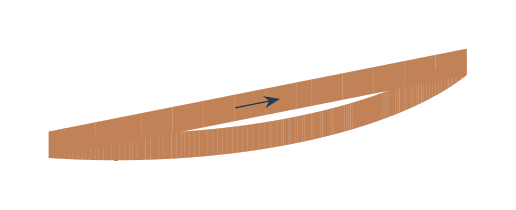
\begin{tikzpicture}[x=9.01059cm,y=9.01059cm]
\path[use as bounding box] (-0.324098,-0.108305) rectangle (0.324098,0.108305);
\path[fill=copper!82,draw=copper!82,line width=.08pt] (-0.198715,-0.078305) -- (-0.202402,-0.078302) -- (-0.202402,-0.041460) -- (-0.198715,-0.041463) -- cycle;
\path[fill=copper!82,draw=copper!82,line width=.08pt] (-0.195028,-0.078298) -- (-0.198715,-0.078305) -- (-0.198715,-0.041463) -- (-0.195028,-0.041455) -- cycle;
\path[fill=copper!82,draw=copper!82,line width=.08pt] (-0.202402,-0.078302) -- (-0.206088,-0.078290) -- (-0.206088,-0.041448) -- (-0.202402,-0.041460) -- cycle;
\path[fill=copper!82,draw=copper!82,line width=.08pt] (-0.191342,-0.078281) -- (-0.195028,-0.078298) -- (-0.195028,-0.041455) -- (-0.191342,-0.041439) -- cycle;
\path[fill=copper!82,draw=copper!82,line width=.08pt] (-0.206088,-0.078290) -- (-0.209775,-0.078268) -- (-0.209775,-0.041426) -- (-0.206088,-0.041448) -- cycle;
\path[fill=copper!82,draw=copper!82,line width=.08pt] (-0.187656,-0.078255) -- (-0.191342,-0.078281) -- (-0.191342,-0.041439) -- (-0.187656,-0.041412) -- cycle;
\path[fill=copper!82,draw=copper!82,line width=.08pt] (-0.209775,-0.078268) -- (-0.213460,-0.078237) -- (-0.213460,-0.041395) -- (-0.209775,-0.041426) -- cycle;
\path[fill=copper!82,draw=copper!82,line width=.08pt] (-0.183970,-0.078219) -- (-0.187656,-0.078255) -- (-0.187656,-0.041412) -- (-0.183970,-0.041376) -- cycle;
\path[fill=copper!82,draw=copper!82,line width=.08pt] (-0.213460,-0.078237) -- (-0.217146,-0.078196) -- (-0.217146,-0.041354) -- (-0.213460,-0.041395) -- cycle;
\path[fill=copper!82,draw=copper!82,line width=.08pt] (-0.180285,-0.078173) -- (-0.183970,-0.078219) -- (-0.183970,-0.041376) -- (-0.180285,-0.041331) -- cycle;
\path[fill=copper!82,draw=copper!82,line width=.08pt] (-0.217146,-0.078196) -- (-0.220830,-0.078145) -- (-0.220830,-0.041303) -- (-0.217146,-0.041354) -- cycle;
\path[fill=copper!82,draw=copper!82,line width=.08pt] (-0.176601,-0.078118) -- (-0.180285,-0.078173) -- (-0.180285,-0.041331) -- (-0.176601,-0.041276) -- cycle;
\path[fill=copper!82,draw=copper!82,line width=.08pt] (-0.220830,-0.078145) -- (-0.224514,-0.078085) -- (-0.224514,-0.041243) -- (-0.220830,-0.041303) -- cycle;
\path[fill=copper!82,draw=copper!82,line width=.08pt] (-0.172918,-0.078053) -- (-0.176601,-0.078118) -- (-0.176601,-0.041276) -- (-0.172918,-0.041211) -- cycle;
\path[fill=copper!82,draw=copper!82,line width=.08pt] (-0.224514,-0.078085) -- (-0.228196,-0.078015) -- (-0.228196,-0.041173) -- (-0.224514,-0.041243) -- cycle;
\path[fill=copper!82,draw=copper!82,line width=.08pt] (-0.169237,-0.077979) -- (-0.172918,-0.078053) -- (-0.172918,-0.041211) -- (-0.169237,-0.041137) -- cycle;
\path[fill=copper!82,draw=copper!82,line width=.08pt] (-0.228196,-0.078015) -- (-0.231877,-0.077936) -- (-0.231877,-0.041093) -- (-0.228196,-0.041173) -- cycle;
\path[fill=copper!82,draw=copper!82,line width=.08pt] (-0.165556,-0.077895) -- (-0.169237,-0.077979) -- (-0.169237,-0.041137) -- (-0.165556,-0.041053) -- cycle;
\path[fill=copper!82,draw=copper!82,line width=.08pt] (-0.231877,-0.077936) -- (-0.235557,-0.077847) -- (-0.235557,-0.041004) -- (-0.231877,-0.041093) -- cycle;
\path[fill=copper!82,draw=copper!82,line width=.08pt] (-0.161877,-0.077801) -- (-0.165556,-0.077895) -- (-0.165556,-0.041053) -- (-0.161877,-0.040959) -- cycle;
\path[fill=copper!82,draw=copper!82,line width=.08pt] (-0.235557,-0.077847) -- (-0.239235,-0.077748) -- (-0.239235,-0.040905) -- (-0.235557,-0.041004) -- cycle;
\path[fill=copper!82,draw=copper!82,line width=.08pt] (-0.158200,-0.077698) -- (-0.161877,-0.077801) -- (-0.161877,-0.040959) -- (-0.158200,-0.040856) -- cycle;
\path[fill=copper!82,draw=copper!82,line width=.08pt] (-0.239235,-0.077748) -- (-0.242911,-0.077640) -- (-0.242911,-0.040797) -- (-0.239235,-0.040905) -- cycle;
\path[fill=copper!82,draw=copper!82,line width=.08pt] (-0.154525,-0.077585) -- (-0.158200,-0.077698) -- (-0.158200,-0.040856) -- (-0.154525,-0.040743) -- cycle;
\path[fill=copper!82,draw=copper!82,line width=.08pt] (-0.242911,-0.077640) -- (-0.246585,-0.077522) -- (-0.246585,-0.040679) -- (-0.242911,-0.040797) -- cycle;
\path[fill=copper!82,draw=copper!82,line width=.08pt] (-0.150852,-0.077463) -- (-0.154525,-0.077585) -- (-0.154525,-0.040743) -- (-0.150852,-0.040620) -- cycle;
\path[fill=copper!82,draw=copper!82,line width=.08pt] (-0.246585,-0.077522) -- (-0.250257,-0.077394) -- (-0.250257,-0.040552) -- (-0.246585,-0.040679) -- cycle;
\path[fill=copper!82,draw=copper!82,line width=.08pt] (-0.147181,-0.077331) -- (-0.150852,-0.077463) -- (-0.150852,-0.040620) -- (-0.147181,-0.040488) -- cycle;
\path[fill=copper!82,draw=copper!82,line width=.08pt] (-0.250257,-0.077394) -- (-0.253927,-0.077257) -- (-0.253927,-0.040415) -- (-0.250257,-0.040552) -- cycle;
\path[fill=copper!82,draw=copper!82,line width=.08pt] (-0.143512,-0.077189) -- (-0.147181,-0.077331) -- (-0.147181,-0.040488) -- (-0.143512,-0.040347) -- cycle;
\path[fill=copper!82,draw=copper!82,line width=.08pt] (-0.253927,-0.077257) -- (-0.257595,-0.077110) -- (-0.257595,-0.040268) -- (-0.253927,-0.040415) -- cycle;
\path[fill=copper!82,draw=copper!82,line width=.08pt] (-0.139846,-0.077038) -- (-0.143512,-0.077189) -- (-0.143512,-0.040347) -- (-0.139846,-0.040196) -- cycle;
\path[fill=copper!82,draw=copper!82,line width=.08pt] (-0.257595,-0.077110) -- (-0.261259,-0.076954) -- (-0.261259,-0.040112) -- (-0.257595,-0.040268) -- cycle;
\path[fill=copper!82,draw=copper!82,line width=.08pt] (-0.136182,-0.076877) -- (-0.139846,-0.077038) -- (-0.139846,-0.040196) -- (-0.136182,-0.040035) -- cycle;
\path[fill=copper!82,draw=copper!82,line width=.08pt] (-0.261259,-0.076954) -- (-0.264921,-0.076788) -- (-0.264921,-0.039946) -- (-0.261259,-0.040112) -- cycle;
\path[fill=copper!82,draw=copper!82,line width=.08pt] (-0.132521,-0.076707) -- (-0.136182,-0.076877) -- (-0.136182,-0.040035) -- (-0.132521,-0.039865) -- cycle;
\path[fill=copper!82,draw=copper!82,line width=.08pt] (-0.264921,-0.076788) -- (-0.268581,-0.076613) -- (-0.268581,-0.039771) -- (-0.264921,-0.039946) -- cycle;
\path[fill=copper!82,draw=copper!82,line width=.08pt] (-0.128864,-0.076527) -- (-0.132521,-0.076707) -- (-0.132521,-0.039865) -- (-0.128864,-0.039685) -- cycle;
\path[fill=copper!82,draw=copper!82,line width=.08pt] (-0.268581,-0.076613) -- (-0.272237,-0.076428) -- (-0.272237,-0.039586) -- (-0.268581,-0.039771) -- cycle;
\path[fill=copper!82,draw=copper!82,line width=.08pt] (-0.125209,-0.076338) -- (-0.128864,-0.076527) -- (-0.128864,-0.039685) -- (-0.125209,-0.039496) -- cycle;
\path[fill=copper!82,draw=copper!82,line width=.08pt] (-0.272237,-0.076428) -- (-0.275889,-0.076234) -- (-0.275889,-0.039391) -- (-0.272237,-0.039586) -- cycle;
\path[fill=copper!82,draw=copper!82,line width=.08pt] (-0.121558,-0.076139) -- (-0.125209,-0.076338) -- (-0.125209,-0.039496) -- (-0.121558,-0.039297) -- cycle;
\path[fill=copper!82,draw=copper!82,line width=.08pt] (-0.275889,-0.076234) -- (-0.279539,-0.076030) -- (-0.279539,-0.039187) -- (-0.275889,-0.039391) -- cycle;
\path[fill=copper!82,draw=copper!82,line width=.08pt] (-0.117910,-0.075931) -- (-0.121558,-0.076139) -- (-0.121558,-0.039297) -- (-0.117910,-0.039088) -- cycle;
\path[fill=copper!82,draw=copper!82,line width=.08pt] (-0.279539,-0.076030) -- (-0.283184,-0.075816) -- (-0.283184,-0.038974) -- (-0.279539,-0.039187) -- cycle;
\path[fill=copper!82,draw=copper!82,line width=.08pt] (-0.114266,-0.075713) -- (-0.117910,-0.075931) -- (-0.117910,-0.039088) -- (-0.114266,-0.038870) -- cycle;
\path[fill=copper!82,draw=copper!82,line width=.08pt] (-0.283184,-0.075816) -- (-0.286826,-0.075593) -- (-0.286826,-0.038751) -- (-0.283184,-0.038974) -- cycle;
\path[fill=copper!82,draw=copper!82,line width=.08pt] (-0.110626,-0.075485) -- (-0.114266,-0.075713) -- (-0.114266,-0.038870) -- (-0.110626,-0.038643) -- cycle;
\path[fill=copper!82,draw=copper!82,line width=.08pt] (-0.286826,-0.075593) -- (-0.290464,-0.075361) -- (-0.290464,-0.038519) -- (-0.286826,-0.038751) -- cycle;
\path[fill=copper!82,draw=copper!82,line width=.08pt] (-0.106990,-0.075248) -- (-0.110626,-0.075485) -- (-0.110626,-0.038643) -- (-0.106990,-0.038406) -- cycle;
\path[fill=copper!82,draw=copper!82,line width=.08pt] (-0.290464,-0.075361) -- (-0.294098,-0.075119) -- (-0.294098,-0.038277) -- (-0.290464,-0.038519) -- cycle;
\path[fill=copper!82,draw=copper!82,line width=.08pt] (-0.103358,-0.075002) -- (-0.106990,-0.075248) -- (-0.106990,-0.038406) -- (-0.103358,-0.038159) -- cycle;
\path[fill=copper!82,draw=copper!82,line width=.08pt] (-0.099730,-0.074746) -- (-0.103358,-0.075002) -- (-0.103358,-0.038159) -- (-0.099730,-0.037904) -- cycle;
\path[fill=copper!82,draw=copper!82,line width=.08pt] (-0.096107,-0.074481) -- (-0.099730,-0.074746) -- (-0.099730,-0.037904) -- (-0.096107,-0.037638) -- cycle;
\path[fill=copper!82,draw=copper!82,line width=.08pt] (-0.092489,-0.074206) -- (-0.096107,-0.074481) -- (-0.096107,-0.037638) -- (-0.092489,-0.037363) -- cycle;
\path[fill=copper!82,draw=copper!82,line width=.08pt] (-0.088875,-0.073921) -- (-0.092489,-0.074206) -- (-0.092489,-0.037363) -- (-0.088875,-0.037079) -- cycle;
\path[fill=copper!82,draw=copper!82,line width=.08pt] (-0.085266,-0.073628) -- (-0.088875,-0.073921) -- (-0.088875,-0.037079) -- (-0.085266,-0.036785) -- cycle;
\path[fill=copper!82,draw=copper!82,line width=.08pt] (-0.081662,-0.073325) -- (-0.085266,-0.073628) -- (-0.085266,-0.036785) -- (-0.081662,-0.036482) -- cycle;
\path[fill=copper!82,draw=copper!82,line width=.08pt] (-0.078064,-0.073012) -- (-0.081662,-0.073325) -- (-0.081662,-0.036482) -- (-0.078064,-0.036170) -- cycle;
\path[fill=copper!82,draw=copper!82,line width=.08pt] (-0.294098,-0.075119) -- (-0.272313,-0.070801) -- (-0.272313,-0.033959) -- (-0.294098,-0.038277) -- cycle;
\path[fill=copper!82,draw=copper!82,line width=.08pt] (-0.074471,-0.072690) -- (-0.078064,-0.073012) -- (-0.078064,-0.036170) -- (-0.074471,-0.035848) -- cycle;
\path[fill=copper!82,draw=copper!82,line width=.08pt] (-0.070884,-0.072359) -- (-0.074471,-0.072690) -- (-0.074471,-0.035848) -- (-0.070884,-0.035517) -- cycle;
\path[fill=copper!82,draw=copper!82,line width=.08pt] (-0.067303,-0.072018) -- (-0.070884,-0.072359) -- (-0.070884,-0.035517) -- (-0.067303,-0.035176) -- cycle;
\path[fill=copper!82,draw=copper!82,line width=.08pt] (-0.063727,-0.071668) -- (-0.067303,-0.072018) -- (-0.067303,-0.035176) -- (-0.063727,-0.034826) -- cycle;
\path[fill=copper!82,draw=copper!82,line width=.08pt] (-0.060158,-0.071309) -- (-0.063727,-0.071668) -- (-0.063727,-0.034826) -- (-0.060158,-0.034467) -- cycle;
\path[fill=copper!82,draw=copper!82,line width=.08pt] (-0.056595,-0.070941) -- (-0.060158,-0.071309) -- (-0.060158,-0.034467) -- (-0.056595,-0.034098) -- cycle;
\path[fill=copper!82,draw=copper!82,line width=.08pt] (-0.053038,-0.070563) -- (-0.056595,-0.070941) -- (-0.056595,-0.034098) -- (-0.053038,-0.033720) -- cycle;
\path[fill=copper!82,draw=copper!82,line width=.08pt] (-0.049488,-0.070176) -- (-0.053038,-0.070563) -- (-0.053038,-0.033720) -- (-0.049488,-0.033333) -- cycle;
\path[fill=copper!82,draw=copper!82,line width=.08pt] (-0.045944,-0.069779) -- (-0.049488,-0.070176) -- (-0.049488,-0.033333) -- (-0.045944,-0.032937) -- cycle;
\path[fill=copper!82,draw=copper!82,line width=.08pt] (-0.042408,-0.069373) -- (-0.045944,-0.069779) -- (-0.045944,-0.032937) -- (-0.042408,-0.032531) -- cycle;
\path[fill=copper!82,draw=copper!82,line width=.08pt] (-0.038878,-0.068959) -- (-0.042408,-0.069373) -- (-0.042408,-0.032531) -- (-0.038878,-0.032116) -- cycle;
\path[fill=copper!82,draw=copper!82,line width=.08pt] (-0.035356,-0.068534) -- (-0.038878,-0.068959) -- (-0.038878,-0.032116) -- (-0.035356,-0.031692) -- cycle;
\path[fill=copper!82,draw=copper!82,line width=.08pt] (-0.272313,-0.070801) -- (-0.250528,-0.066483) -- (-0.250528,-0.029641) -- (-0.272313,-0.033959) -- cycle;
\path[fill=copper!82,draw=copper!82,line width=.08pt] (-0.031841,-0.068101) -- (-0.035356,-0.068534) -- (-0.035356,-0.031692) -- (-0.031841,-0.031259) -- cycle;
\path[fill=copper!82,draw=copper!82,line width=.08pt] (-0.028334,-0.067659) -- (-0.031841,-0.068101) -- (-0.031841,-0.031259) -- (-0.028334,-0.030816) -- cycle;
\path[fill=copper!82,draw=copper!82,line width=.08pt] (-0.024835,-0.067207) -- (-0.028334,-0.067659) -- (-0.028334,-0.030816) -- (-0.024835,-0.030365) -- cycle;
\path[fill=copper!82,draw=copper!82,line width=.08pt] (-0.021343,-0.066746) -- (-0.024835,-0.067207) -- (-0.024835,-0.030365) -- (-0.021343,-0.029904) -- cycle;
\path[fill=copper!82,draw=copper!82,line width=.08pt] (-0.017859,-0.066277) -- (-0.021343,-0.066746) -- (-0.021343,-0.029904) -- (-0.017859,-0.029434) -- cycle;
\path[fill=copper!82,draw=copper!82,line width=.08pt] (-0.014383,-0.065798) -- (-0.017859,-0.066277) -- (-0.017859,-0.029434) -- (-0.014383,-0.028955) -- cycle;
\path[fill=copper!82,draw=copper!82,line width=.08pt] (-0.010916,-0.065310) -- (-0.014383,-0.065798) -- (-0.014383,-0.028955) -- (-0.010916,-0.028467) -- cycle;
\path[fill=copper!82,draw=copper!82,line width=.08pt] (-0.007457,-0.064813) -- (-0.010916,-0.065310) -- (-0.010916,-0.028467) -- (-0.007457,-0.027970) -- cycle;
\path[fill=copper!82,draw=copper!82,line width=.08pt] (-0.004007,-0.064307) -- (-0.007457,-0.064813) -- (-0.007457,-0.027970) -- (-0.004007,-0.027464) -- cycle;
\path[fill=copper!82,draw=copper!82,line width=.08pt] (-0.250528,-0.066483) -- (-0.228743,-0.062165) -- (-0.228743,-0.025323) -- (-0.250528,-0.029641) -- cycle;
\path[fill=copper!82,draw=copper!82,line width=.08pt] (-0.000566,-0.063792) -- (-0.004007,-0.064307) -- (-0.004007,-0.027464) -- (-0.000566,-0.026949) -- cycle;
\path[fill=copper!82,draw=copper!82,line width=.08pt] (0.002866,-0.063268) -- (-0.000566,-0.063792) -- (-0.000566,-0.026949) -- (0.002866,-0.026425) -- cycle;
\path[fill=copper!82,draw=copper!82,line width=.08pt] (0.006290,-0.062735) -- (0.002866,-0.063268) -- (0.002866,-0.026425) -- (0.006290,-0.025892) -- cycle;
\path[fill=copper!82,draw=copper!82,line width=.08pt] (0.009704,-0.062193) -- (0.006290,-0.062735) -- (0.006290,-0.025892) -- (0.009704,-0.025351) -- cycle;
\path[fill=copper!82,draw=copper!82,line width=.08pt] (0.013108,-0.061642) -- (0.009704,-0.062193) -- (0.009704,-0.025351) -- (0.013108,-0.024800) -- cycle;
\path[fill=copper!82,draw=copper!82,line width=.08pt] (0.016504,-0.061083) -- (0.013108,-0.061642) -- (0.013108,-0.024800) -- (0.016504,-0.024240) -- cycle;
\path[fill=copper!82,draw=copper!82,line width=.08pt] (0.019889,-0.060514) -- (0.016504,-0.061083) -- (0.016504,-0.024240) -- (0.019889,-0.023672) -- cycle;
\path[fill=copper!82,draw=copper!82,line width=.08pt] (0.023264,-0.059937) -- (0.019889,-0.060514) -- (0.019889,-0.023672) -- (0.023264,-0.023094) -- cycle;
\path[fill=copper!82,draw=copper!82,line width=.08pt] (-0.228743,-0.062165) -- (-0.206958,-0.057848) -- (-0.206958,-0.021005) -- (-0.228743,-0.025323) -- cycle;
\path[fill=copper!82,draw=copper!82,line width=.08pt] (0.026630,-0.059351) -- (0.023264,-0.059937) -- (0.023264,-0.023094) -- (0.026630,-0.022508) -- cycle;
\path[fill=copper!82,draw=copper!82,line width=.08pt] (0.029985,-0.058756) -- (0.026630,-0.059351) -- (0.026630,-0.022508) -- (0.029985,-0.021913) -- cycle;
\path[fill=copper!82,draw=copper!82,line width=.08pt] (0.033330,-0.058152) -- (0.029985,-0.058756) -- (0.029985,-0.021913) -- (0.033330,-0.021310) -- cycle;
\path[fill=copper!82,draw=copper!82,line width=.08pt] (0.036665,-0.057540) -- (0.033330,-0.058152) -- (0.033330,-0.021310) -- (0.036665,-0.020698) -- cycle;
\path[fill=copper!82,draw=copper!82,line width=.08pt] (0.039989,-0.056919) -- (0.036665,-0.057540) -- (0.036665,-0.020698) -- (0.039989,-0.020076) -- cycle;
\path[fill=copper!82,draw=copper!82,line width=.08pt] (0.043302,-0.056289) -- (0.039989,-0.056919) -- (0.039989,-0.020076) -- (0.043302,-0.019447) -- cycle;
\path[fill=copper!82,draw=copper!82,line width=.08pt] (0.046604,-0.055651) -- (0.043302,-0.056289) -- (0.043302,-0.019447) -- (0.046604,-0.018808) -- cycle;
\path[fill=copper!82,draw=copper!82,line width=.08pt] (-0.206958,-0.057848) -- (-0.185173,-0.053530) -- (-0.185173,-0.016687) -- (-0.206958,-0.021005) -- cycle;
\path[fill=copper!82,draw=copper!82,line width=.08pt] (0.049896,-0.055004) -- (0.046604,-0.055651) -- (0.046604,-0.018808) -- (0.049896,-0.018162) -- cycle;
\path[fill=copper!82,draw=copper!82,line width=.08pt] (0.053176,-0.054349) -- (0.049896,-0.055004) -- (0.049896,-0.018162) -- (0.053176,-0.017506) -- cycle;
\path[fill=copper!82,draw=copper!82,line width=.08pt] (0.056444,-0.053684) -- (0.053176,-0.054349) -- (0.053176,-0.017506) -- (0.056444,-0.016842) -- cycle;
\path[fill=copper!82,draw=copper!82,line width=.08pt] (0.059701,-0.053012) -- (0.056444,-0.053684) -- (0.056444,-0.016842) -- (0.059701,-0.016169) -- cycle;
\path[fill=copper!82,draw=copper!82,line width=.08pt] (0.062947,-0.052331) -- (0.059701,-0.053012) -- (0.059701,-0.016169) -- (0.062947,-0.015488) -- cycle;
\path[fill=copper!82,draw=copper!82,line width=.08pt] (0.066181,-0.051641) -- (0.062947,-0.052331) -- (0.062947,-0.015488) -- (0.066181,-0.014799) -- cycle;
\path[fill=copper!82,draw=copper!82,line width=.08pt] (-0.185173,-0.053530) -- (-0.163388,-0.049212) -- (-0.163388,-0.012370) -- (-0.185173,-0.016687) -- cycle;
\path[fill=copper!82,draw=copper!82,line width=.08pt] (0.069402,-0.050943) -- (0.066181,-0.051641) -- (0.066181,-0.014799) -- (0.069402,-0.014101) -- cycle;
\path[fill=copper!82,draw=copper!82,line width=.08pt] (0.072612,-0.050237) -- (0.069402,-0.050943) -- (0.069402,-0.014101) -- (0.072612,-0.013395) -- cycle;
\path[fill=copper!82,draw=copper!82,line width=.08pt] (0.075809,-0.049522) -- (0.072612,-0.050237) -- (0.072612,-0.013395) -- (0.075809,-0.012680) -- cycle;
\path[fill=copper!82,draw=copper!82,line width=.08pt] (0.078995,-0.048799) -- (0.075809,-0.049522) -- (0.075809,-0.012680) -- (0.078995,-0.011957) -- cycle;
\path[fill=copper!82,draw=copper!82,line width=.08pt] (0.082167,-0.048068) -- (0.078995,-0.048799) -- (0.078995,-0.011957) -- (0.082167,-0.011226) -- cycle;
\path[fill=copper!82,draw=copper!82,line width=.08pt] (0.085327,-0.047328) -- (0.082167,-0.048068) -- (0.082167,-0.011226) -- (0.085327,-0.010486) -- cycle;
\path[fill=copper!82,draw=copper!82,line width=.08pt] (-0.163388,-0.049212) -- (-0.141603,-0.044894) -- (-0.141603,-0.008052) -- (-0.163388,-0.012370) -- cycle;
\path[fill=copper!82,draw=copper!82,line width=.08pt] (0.088474,-0.046581) -- (0.085327,-0.047328) -- (0.085327,-0.010486) -- (0.088474,-0.009738) -- cycle;
\path[fill=copper!82,draw=copper!82,line width=.08pt] (0.091608,-0.045825) -- (0.088474,-0.046581) -- (0.088474,-0.009738) -- (0.091608,-0.008982) -- cycle;
\path[fill=copper!82,draw=copper!82,line width=.08pt] (0.094729,-0.045060) -- (0.091608,-0.045825) -- (0.091608,-0.008982) -- (0.094729,-0.008218) -- cycle;
\path[fill=copper!82,draw=copper!82,line width=.08pt] (0.097837,-0.044288) -- (0.094729,-0.045060) -- (0.094729,-0.008218) -- (0.097837,-0.007446) -- cycle;
\path[fill=copper!82,draw=copper!82,line width=.08pt] (0.100932,-0.043508) -- (0.097837,-0.044288) -- (0.097837,-0.007446) -- (0.100932,-0.006665) -- cycle;
\path[fill=copper!82,draw=copper!82,line width=.08pt] (0.104013,-0.042719) -- (0.100932,-0.043508) -- (0.100932,-0.006665) -- (0.104013,-0.005877) -- cycle;
\path[fill=copper!82,draw=copper!82,line width=.08pt] (-0.141603,-0.044894) -- (-0.119818,-0.040576) -- (-0.119818,-0.003734) -- (-0.141603,-0.008052) -- cycle;
\path[fill=copper!82,draw=copper!82,line width=.08pt] (0.107080,-0.041923) -- (0.104013,-0.042719) -- (0.104013,-0.005877) -- (0.107080,-0.005080) -- cycle;
\path[fill=copper!82,draw=copper!82,line width=.08pt] (0.110133,-0.041118) -- (0.107080,-0.041923) -- (0.107080,-0.005080) -- (0.110133,-0.004276) -- cycle;
\path[fill=copper!82,draw=copper!82,line width=.08pt] (0.113173,-0.040306) -- (0.110133,-0.041118) -- (0.110133,-0.004276) -- (0.113173,-0.003463) -- cycle;
\path[fill=copper!82,draw=copper!82,line width=.08pt] (0.116199,-0.039486) -- (0.113173,-0.040306) -- (0.113173,-0.003463) -- (0.116199,-0.002643) -- cycle;
\path[fill=copper!82,draw=copper!82,line width=.08pt] (0.119210,-0.038657) -- (0.116199,-0.039486) -- (0.116199,-0.002643) -- (0.119210,-0.001815) -- cycle;
\path[fill=copper!82,draw=copper!82,line width=.08pt] (-0.119818,-0.040576) -- (-0.098033,-0.036258) -- (-0.098033,0.000584) -- (-0.119818,-0.003734) -- cycle;
\path[fill=copper!82,draw=copper!82,line width=.08pt] (0.122207,-0.037821) -- (0.119210,-0.038657) -- (0.119210,-0.001815) -- (0.122207,-0.000979) -- cycle;
\path[fill=copper!82,draw=copper!82,line width=.08pt] (0.125190,-0.036977) -- (0.122207,-0.037821) -- (0.122207,-0.000979) -- (0.125190,-0.000135) -- cycle;
\path[fill=copper!82,draw=copper!82,line width=.08pt] (0.128158,-0.036126) -- (0.125190,-0.036977) -- (0.125190,-0.000135) -- (0.128158,0.000717) -- cycle;
\path[fill=copper!82,draw=copper!82,line width=.08pt] (0.131111,-0.035266) -- (0.128158,-0.036126) -- (0.128158,0.000717) -- (0.131111,0.001576) -- cycle;
\path[fill=copper!82,draw=copper!82,line width=.08pt] (0.134050,-0.034399) -- (0.131111,-0.035266) -- (0.131111,0.001576) -- (0.134050,0.002443) -- cycle;
\path[fill=copper!82,draw=copper!82,line width=.08pt] (-0.098033,-0.036258) -- (-0.076248,-0.031941) -- (-0.076248,0.004902) -- (-0.098033,0.000584) -- cycle;
\path[fill=copper!82,draw=copper!82,line width=.08pt] (0.136973,-0.033525) -- (0.134050,-0.034399) -- (0.134050,0.002443) -- (0.136973,0.003318) -- cycle;
\path[fill=copper!82,draw=copper!82,line width=.08pt] (0.139881,-0.032642) -- (0.136973,-0.033525) -- (0.136973,0.003318) -- (0.139881,0.004200) -- cycle;
\path[fill=copper!82,draw=copper!82,line width=.08pt] (0.142774,-0.031752) -- (0.139881,-0.032642) -- (0.139881,0.004200) -- (0.142774,0.005090) -- cycle;
\path[fill=copper!82,draw=copper!82,line width=.08pt] (0.145652,-0.030855) -- (0.142774,-0.031752) -- (0.142774,0.005090) -- (0.145652,0.005987) -- cycle;
\path[fill=copper!82,draw=copper!82,line width=.08pt] (0.148514,-0.029950) -- (0.145652,-0.030855) -- (0.145652,0.005987) -- (0.148514,0.006892) -- cycle;
\path[fill=copper!82,draw=copper!82,line width=.08pt] (-0.076248,-0.031941) -- (-0.054463,-0.027623) -- (-0.054463,0.009220) -- (-0.076248,0.004902) -- cycle;
\path[fill=copper!82,draw=copper!82,line width=.08pt] (0.151361,-0.029038) -- (0.148514,-0.029950) -- (0.148514,0.006892) -- (0.151361,0.007805) -- cycle;
\path[fill=copper!82,draw=copper!82,line width=.08pt] (0.154192,-0.028118) -- (0.151361,-0.029038) -- (0.151361,0.007805) -- (0.154192,0.008725) -- cycle;
\path[fill=copper!82,draw=copper!82,line width=.08pt] (0.157006,-0.027191) -- (0.154192,-0.028118) -- (0.154192,0.008725) -- (0.157006,0.009652) -- cycle;
\path[fill=copper!82,draw=copper!82,line width=.08pt] (0.159805,-0.026256) -- (0.157006,-0.027191) -- (0.157006,0.009652) -- (0.159805,0.010586) -- cycle;
\path[fill=copper!82,draw=copper!82,line width=.08pt] (0.162588,-0.025315) -- (0.159805,-0.026256) -- (0.159805,0.010586) -- (0.162588,0.011528) -- cycle;
\path[fill=copper!82,draw=copper!82,line width=.08pt] (-0.054463,-0.027623) -- (-0.032678,-0.023305) -- (-0.032678,0.013537) -- (-0.054463,0.009220) -- cycle;
\path[fill=copper!82,draw=copper!82,line width=.08pt] (0.165354,-0.024366) -- (0.162588,-0.025315) -- (0.162588,0.011528) -- (0.165354,0.012477) -- cycle;
\path[fill=copper!82,draw=copper!82,line width=.08pt] (0.168104,-0.023409) -- (0.165354,-0.024366) -- (0.165354,0.012477) -- (0.168104,0.013433) -- cycle;
\path[fill=copper!82,draw=copper!82,line width=.08pt] (0.170838,-0.022446) -- (0.168104,-0.023409) -- (0.168104,0.013433) -- (0.170838,0.014396) -- cycle;
\path[fill=copper!82,draw=copper!82,line width=.08pt] (0.173555,-0.021476) -- (0.170838,-0.022446) -- (0.170838,0.014396) -- (0.173555,0.015367) -- cycle;
\path[fill=copper!82,draw=copper!82,line width=.08pt] (-0.032678,-0.023305) -- (-0.010893,-0.018987) -- (-0.010893,0.017855) -- (-0.032678,0.013537) -- cycle;
\path[fill=copper!82,draw=copper!82,line width=.08pt] (0.176255,-0.020498) -- (0.173555,-0.021476) -- (0.173555,0.015367) -- (0.176255,0.016344) -- cycle;
\path[fill=copper!82,draw=copper!82,line width=.08pt] (0.178938,-0.019513) -- (0.176255,-0.020498) -- (0.176255,0.016344) -- (0.178938,0.017329) -- cycle;
\path[fill=copper!82,draw=copper!82,line width=.08pt] (0.181604,-0.018522) -- (0.178938,-0.019513) -- (0.178938,0.017329) -- (0.181604,0.018321) -- cycle;
\path[fill=copper!82,draw=copper!82,line width=.08pt] (0.184253,-0.017523) -- (0.181604,-0.018522) -- (0.181604,0.018321) -- (0.184253,0.019319) -- cycle;
\path[fill=copper!82,draw=copper!82,line width=.08pt] (0.186885,-0.016518) -- (0.184253,-0.017523) -- (0.184253,0.019319) -- (0.186885,0.020324) -- cycle;
\path[fill=copper!82,draw=copper!82,line width=.08pt] (-0.010893,-0.018987) -- (0.010893,-0.014669) -- (0.010893,0.022173) -- (-0.010893,0.017855) -- cycle;
\path[fill=copper!82,draw=copper!82,line width=.08pt] (0.189500,-0.015506) -- (0.186885,-0.016518) -- (0.186885,0.020324) -- (0.189500,0.021337) -- cycle;
\path[fill=copper!82,draw=copper!82,line width=.08pt] (0.192097,-0.014487) -- (0.189500,-0.015506) -- (0.189500,0.021337) -- (0.192097,0.022356) -- cycle;
\path[fill=copper!82,draw=copper!82,line width=.08pt] (0.194676,-0.013461) -- (0.192097,-0.014487) -- (0.192097,0.022356) -- (0.194676,0.023381) -- cycle;
\path[fill=copper!82,draw=copper!82,line width=.08pt] (0.197238,-0.012429) -- (0.194676,-0.013461) -- (0.194676,0.023381) -- (0.197238,0.024414) -- cycle;
\path[fill=copper!82,draw=copper!82,line width=.08pt] (0.010893,-0.014669) -- (0.032678,-0.010351) -- (0.032678,0.026491) -- (0.010893,0.022173) -- cycle;
\path[fill=copper!82,draw=copper!82,line width=.08pt] (0.199782,-0.011389) -- (0.197238,-0.012429) -- (0.197238,0.024414) -- (0.199782,0.025453) -- cycle;
\path[fill=copper!82,draw=copper!82,line width=.08pt] (0.202307,-0.010344) -- (0.199782,-0.011389) -- (0.199782,0.025453) -- (0.202307,0.026499) -- cycle;
\path[fill=copper!82,draw=copper!82,line width=.08pt] (0.204815,-0.009291) -- (0.202307,-0.010344) -- (0.202307,0.026499) -- (0.204815,0.027551) -- cycle;
\path[fill=copper!82,draw=copper!82,line width=.08pt] (0.207305,-0.008232) -- (0.204815,-0.009291) -- (0.204815,0.027551) -- (0.207305,0.028610) -- cycle;
\path[fill=copper!82,draw=copper!82,line width=.08pt] (0.032678,-0.010351) -- (0.054463,-0.006034) -- (0.054463,0.030809) -- (0.032678,0.026491) -- cycle;
\path[fill=copper!82,draw=copper!82,line width=.08pt] (0.209776,-0.007167) -- (0.207305,-0.008232) -- (0.207305,0.028610) -- (0.209776,0.029675) -- cycle;
\path[fill=copper!82,draw=copper!82,line width=.08pt] (0.212229,-0.006095) -- (0.209776,-0.007167) -- (0.209776,0.029675) -- (0.212229,0.030747) -- cycle;
\path[fill=copper!82,draw=copper!82,line width=.08pt] (0.214664,-0.005017) -- (0.212229,-0.006095) -- (0.212229,0.030747) -- (0.214664,0.031825) -- cycle;
\path[fill=copper!82,draw=copper!82,line width=.08pt] (0.217080,-0.003933) -- (0.214664,-0.005017) -- (0.214664,0.031825) -- (0.217080,0.032910) -- cycle;
\path[fill=copper!82,draw=copper!82,line width=.08pt] (0.054463,-0.006034) -- (0.076248,-0.001716) -- (0.076248,0.035127) -- (0.054463,0.030809) -- cycle;
\path[fill=copper!82,draw=copper!82,line width=.08pt] (0.219477,-0.002842) -- (0.217080,-0.003933) -- (0.217080,0.032910) -- (0.219477,0.034000) -- cycle;
\path[fill=copper!82,draw=copper!82,line width=.08pt] (0.221855,-0.001745) -- (0.219477,-0.002842) -- (0.219477,0.034000) -- (0.221855,0.035097) -- cycle;
\path[fill=copper!82,draw=copper!82,line width=.08pt] (0.224215,-0.000642) -- (0.221855,-0.001745) -- (0.221855,0.035097) -- (0.224215,0.036201) -- cycle;
\path[fill=copper!82,draw=copper!82,line width=.08pt] (0.226555,0.000468) -- (0.224215,-0.000642) -- (0.224215,0.036201) -- (0.226555,0.037310) -- cycle;
\path[fill=copper!82,draw=copper!82,line width=.08pt] (0.076248,-0.001716) -- (0.098033,0.002602) -- (0.098033,0.039444) -- (0.076248,0.035127) -- cycle;
\path[fill=copper!82,draw=copper!82,line width=.08pt] (0.228876,0.001583) -- (0.226555,0.000468) -- (0.226555,0.037310) -- (0.228876,0.038425) -- cycle;
\path[fill=copper!82,draw=copper!82,line width=.08pt] (0.231178,0.002704) -- (0.228876,0.001583) -- (0.228876,0.038425) -- (0.231178,0.039547) -- cycle;
\path[fill=copper!82,draw=copper!82,line width=.08pt] (0.233461,0.003832) -- (0.231178,0.002704) -- (0.231178,0.039547) -- (0.233461,0.040674) -- cycle;
\path[fill=copper!82,draw=copper!82,line width=.08pt] (0.235724,0.004965) -- (0.233461,0.003832) -- (0.233461,0.040674) -- (0.235724,0.041808) -- cycle;
\path[fill=copper!82,draw=copper!82,line width=.08pt] (0.098033,0.002602) -- (0.119818,0.006920) -- (0.119818,0.043762) -- (0.098033,0.039444) -- cycle;
\path[fill=copper!82,draw=copper!82,line width=.08pt] (0.237967,0.006104) -- (0.235724,0.004965) -- (0.235724,0.041808) -- (0.237967,0.042947) -- cycle;
\path[fill=copper!82,draw=copper!82,line width=.08pt] (0.240191,0.007249) -- (0.237967,0.006104) -- (0.237967,0.042947) -- (0.240191,0.044092) -- cycle;
\path[fill=copper!82,draw=copper!82,line width=.08pt] (0.242396,0.008400) -- (0.240191,0.007249) -- (0.240191,0.044092) -- (0.242396,0.045243) -- cycle;
\path[fill=copper!82,draw=copper!82,line width=.08pt] (0.244580,0.009557) -- (0.242396,0.008400) -- (0.242396,0.045243) -- (0.244580,0.046399) -- cycle;
\path[fill=copper!82,draw=copper!82,line width=.08pt] (0.119818,0.006920) -- (0.141603,0.011238) -- (0.141603,0.048080) -- (0.119818,0.043762) -- cycle;
\path[fill=copper!82,draw=copper!82,line width=.08pt] (0.246744,0.010719) -- (0.244580,0.009557) -- (0.244580,0.046399) -- (0.246744,0.047561) -- cycle;
\path[fill=copper!82,draw=copper!82,line width=.08pt] (0.248888,0.011887) -- (0.246744,0.010719) -- (0.246744,0.047561) -- (0.248888,0.048729) -- cycle;
\path[fill=copper!82,draw=copper!82,line width=.08pt] (0.251013,0.013060) -- (0.248888,0.011887) -- (0.248888,0.048729) -- (0.251013,0.049903) -- cycle;
\path[fill=copper!82,draw=copper!82,line width=.08pt] (0.141603,0.011238) -- (0.163388,0.015556) -- (0.163388,0.052398) -- (0.141603,0.048080) -- cycle;
\path[fill=copper!82,draw=copper!82,line width=.08pt] (0.253116,0.014239) -- (0.251013,0.013060) -- (0.251013,0.049903) -- (0.253116,0.051082) -- cycle;
\path[fill=copper!82,draw=copper!82,line width=.08pt] (0.255200,0.015424) -- (0.253116,0.014239) -- (0.253116,0.051082) -- (0.255200,0.052266) -- cycle;
\path[fill=copper!82,draw=copper!82,line width=.08pt] (0.257263,0.016613) -- (0.255200,0.015424) -- (0.255200,0.052266) -- (0.257263,0.053456) -- cycle;
\path[fill=copper!82,draw=copper!82,line width=.08pt] (0.259306,0.017809) -- (0.257263,0.016613) -- (0.257263,0.053456) -- (0.259306,0.054651) -- cycle;
\path[fill=copper!82,draw=copper!82,line width=.08pt] (0.163388,0.015556) -- (0.185173,0.019873) -- (0.185173,0.056716) -- (0.163388,0.052398) -- cycle;
\path[fill=copper!82,draw=copper!82,line width=.08pt] (0.261328,0.019009) -- (0.259306,0.017809) -- (0.259306,0.054651) -- (0.261328,0.055852) -- cycle;
\path[fill=copper!82,draw=copper!82,line width=.08pt] (0.263329,0.020215) -- (0.261328,0.019009) -- (0.261328,0.055852) -- (0.263329,0.057057) -- cycle;
\path[fill=copper!82,draw=copper!82,line width=.08pt] (0.265309,0.021426) -- (0.263329,0.020215) -- (0.263329,0.057057) -- (0.265309,0.058268) -- cycle;
\path[fill=copper!82,draw=copper!82,line width=.08pt] (0.185173,0.019873) -- (0.206958,0.024191) -- (0.206958,0.061034) -- (0.185173,0.056716) -- cycle;
\path[fill=copper!82,draw=copper!82,line width=.08pt] (0.267269,0.022642) -- (0.265309,0.021426) -- (0.265309,0.058268) -- (0.267269,0.059484) -- cycle;
\path[fill=copper!82,draw=copper!82,line width=.08pt] (0.269208,0.023863) -- (0.267269,0.022642) -- (0.267269,0.059484) -- (0.269208,0.060706) -- cycle;
\path[fill=copper!82,draw=copper!82,line width=.08pt] (0.271125,0.025089) -- (0.269208,0.023863) -- (0.269208,0.060706) -- (0.271125,0.061932) -- cycle;
\path[fill=copper!82,draw=copper!82,line width=.08pt] (0.273022,0.026320) -- (0.271125,0.025089) -- (0.271125,0.061932) -- (0.273022,0.063163) -- cycle;
\path[fill=copper!82,draw=copper!82,line width=.08pt] (0.206958,0.024191) -- (0.228743,0.028509) -- (0.228743,0.065351) -- (0.206958,0.061034) -- cycle;
\path[fill=copper!82,draw=copper!82,line width=.08pt] (0.274897,0.027557) -- (0.273022,0.026320) -- (0.273022,0.063163) -- (0.274897,0.064399) -- cycle;
\path[fill=copper!82,draw=copper!82,line width=.08pt] (0.276751,0.028798) -- (0.274897,0.027557) -- (0.274897,0.064399) -- (0.276751,0.065640) -- cycle;
\path[fill=copper!82,draw=copper!82,line width=.08pt] (0.278583,0.030043) -- (0.276751,0.028798) -- (0.276751,0.065640) -- (0.278583,0.066886) -- cycle;
\path[fill=copper!82,draw=copper!82,line width=.08pt] (0.228743,0.028509) -- (0.250528,0.032827) -- (0.250528,0.069669) -- (0.228743,0.065351) -- cycle;
\path[fill=copper!82,draw=copper!82,line width=.08pt] (0.280394,0.031294) -- (0.278583,0.030043) -- (0.278583,0.066886) -- (0.280394,0.068136) -- cycle;
\path[fill=copper!82,draw=copper!82,line width=.08pt] (0.282183,0.032549) -- (0.280394,0.031294) -- (0.280394,0.068136) -- (0.282183,0.069392) -- cycle;
\path[fill=copper!82,draw=copper!82,line width=.08pt] (0.283951,0.033809) -- (0.282183,0.032549) -- (0.282183,0.069392) -- (0.283951,0.070651) -- cycle;
\path[fill=copper!82,draw=copper!82,line width=.08pt] (0.285697,0.035073) -- (0.283951,0.033809) -- (0.283951,0.070651) -- (0.285697,0.071916) -- cycle;
\path[fill=copper!82,draw=copper!82,line width=.08pt] (0.250528,0.032827) -- (0.272313,0.037145) -- (0.272313,0.073987) -- (0.250528,0.069669) -- cycle;
\path[fill=copper!82,draw=copper!82,line width=.08pt] (0.287421,0.036342) -- (0.285697,0.035073) -- (0.285697,0.071916) -- (0.287421,0.073185) -- cycle;
\path[fill=copper!82,draw=copper!82,line width=.08pt] (0.289124,0.037616) -- (0.287421,0.036342) -- (0.287421,0.073185) -- (0.289124,0.074458) -- cycle;
\path[fill=copper!82,draw=copper!82,line width=.08pt] (0.290804,0.038894) -- (0.289124,0.037616) -- (0.289124,0.074458) -- (0.290804,0.075736) -- cycle;
\path[fill=copper!82,draw=copper!82,line width=.08pt] (0.272313,0.037145) -- (0.294098,0.041463) -- (0.294098,0.078305) -- (0.272313,0.073987) -- cycle;
\path[fill=copper!82,draw=copper!82,line width=.08pt] (0.292462,0.040176) -- (0.290804,0.038894) -- (0.290804,0.075736) -- (0.292462,0.077018) -- cycle;
\path[fill=copper!82,draw=copper!82,line width=.08pt] (0.294098,0.041463) -- (0.292462,0.040176) -- (0.292462,0.077018) -- (0.294098,0.078305) -- cycle;
\draw[-{Stealth[length=2mm]},navy,line width=.45pt] (-0.031389,-0.004628) -- (0.031389,0.007814);
\end{tikzpicture}
}

\newcommand{\AntennaFigureK}{%
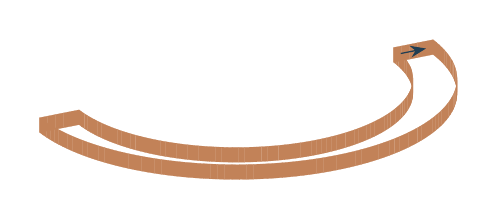
\begin{tikzpicture}[x=5.09557cm,y=5.09557cm]
\path[use as bounding box] (-0.550060,-0.204078) rectangle (0.550060,0.204078);
\path[fill=copper!82,draw=copper!82,line width=.08pt] (-0.022940,-0.174078) -- (-0.040938,-0.174052) -- (-0.040938,-0.137210) -- (-0.022940,-0.137236) -- cycle;
\path[fill=copper!82,draw=copper!82,line width=.08pt] (-0.004950,-0.173875) -- (-0.022940,-0.174078) -- (-0.022940,-0.137236) -- (-0.004950,-0.137033) -- cycle;
\path[fill=copper!82,draw=copper!82,line width=.08pt] (-0.040938,-0.174052) -- (-0.058924,-0.173797) -- (-0.058924,-0.136955) -- (-0.040938,-0.137210) -- cycle;
\path[fill=copper!82,draw=copper!82,line width=.08pt] (0.013014,-0.173443) -- (-0.004950,-0.173875) -- (-0.004950,-0.137033) -- (0.013014,-0.136600) -- cycle;
\path[fill=copper!82,draw=copper!82,line width=.08pt] (-0.058924,-0.173797) -- (-0.076879,-0.173313) -- (-0.076879,-0.136470) -- (-0.058924,-0.136955) -- cycle;
\path[fill=copper!82,draw=copper!82,line width=.08pt] (0.030932,-0.172782) -- (0.013014,-0.173443) -- (0.013014,-0.136600) -- (0.030932,-0.135939) -- cycle;
\path[fill=copper!82,draw=copper!82,line width=.08pt] (-0.076879,-0.173313) -- (-0.094783,-0.172600) -- (-0.094783,-0.135757) -- (-0.076879,-0.136470) -- cycle;
\path[fill=copper!82,draw=copper!82,line width=.08pt] (0.048784,-0.171893) -- (0.030932,-0.172782) -- (0.030932,-0.135939) -- (0.048784,-0.135050) -- cycle;
\path[fill=copper!82,draw=copper!82,line width=.08pt] (-0.094783,-0.172600) -- (-0.112618,-0.171659) -- (-0.112618,-0.134817) -- (-0.094783,-0.135757) -- cycle;
\path[fill=copper!82,draw=copper!82,line width=.08pt] (0.066552,-0.170777) -- (0.048784,-0.171893) -- (0.048784,-0.135050) -- (0.066552,-0.133934) -- cycle;
\path[fill=copper!82,draw=copper!82,line width=.08pt] (-0.112618,-0.171659) -- (-0.130365,-0.170492) -- (-0.130365,-0.133649) -- (-0.112618,-0.134817) -- cycle;
\path[fill=copper!82,draw=copper!82,line width=.08pt] (0.084217,-0.169435) -- (0.066552,-0.170777) -- (0.066552,-0.133934) -- (0.084217,-0.132592) -- cycle;
\path[fill=copper!82,draw=copper!82,line width=.08pt] (-0.130365,-0.170492) -- (-0.148004,-0.169099) -- (-0.148004,-0.132256) -- (-0.130365,-0.133649) -- cycle;
\path[fill=copper!82,draw=copper!82,line width=.08pt] (0.101760,-0.167869) -- (0.084217,-0.169435) -- (0.084217,-0.132592) -- (0.101760,-0.131026) -- cycle;
\path[fill=copper!82,draw=copper!82,line width=.08pt] (-0.148004,-0.169099) -- (-0.165516,-0.167482) -- (-0.165516,-0.130640) -- (-0.148004,-0.132256) -- cycle;
\path[fill=copper!82,draw=copper!82,line width=.08pt] (0.119162,-0.166080) -- (0.101760,-0.167869) -- (0.101760,-0.131026) -- (0.119162,-0.129237) -- cycle;
\path[fill=copper!82,draw=copper!82,line width=.08pt] (-0.165516,-0.167482) -- (-0.182883,-0.165643) -- (-0.182883,-0.128800) -- (-0.165516,-0.130640) -- cycle;
\path[fill=copper!82,draw=copper!82,line width=.08pt] (0.136404,-0.164070) -- (0.119162,-0.166080) -- (0.119162,-0.129237) -- (0.136404,-0.127228) -- cycle;
\path[fill=copper!82,draw=copper!82,line width=.08pt] (-0.182883,-0.165643) -- (-0.200087,-0.163583) -- (-0.200087,-0.126741) -- (-0.182883,-0.128800) -- cycle;
\path[fill=copper!82,draw=copper!82,line width=.08pt] (0.153468,-0.161842) -- (0.136404,-0.164070) -- (0.136404,-0.127228) -- (0.153468,-0.125000) -- cycle;
\path[fill=copper!82,draw=copper!82,line width=.08pt] (-0.200087,-0.163583) -- (-0.217108,-0.161306) -- (-0.217108,-0.124463) -- (-0.200087,-0.126741) -- cycle;
\path[fill=copper!82,draw=copper!82,line width=.08pt] (0.170336,-0.159398) -- (0.153468,-0.161842) -- (0.153468,-0.125000) -- (0.170336,-0.122555) -- cycle;
\path[fill=copper!82,draw=copper!82,line width=.08pt] (-0.217108,-0.161306) -- (-0.233929,-0.158813) -- (-0.233929,-0.121970) -- (-0.217108,-0.124463) -- cycle;
\path[fill=copper!82,draw=copper!82,line width=.08pt] (0.186989,-0.156740) -- (0.170336,-0.159398) -- (0.170336,-0.122555) -- (0.186989,-0.119897) -- cycle;
\path[fill=copper!82,draw=copper!82,line width=.08pt] (-0.233929,-0.158813) -- (-0.250531,-0.156107) -- (-0.250531,-0.119264) -- (-0.233929,-0.121970) -- cycle;
\path[fill=copper!82,draw=copper!82,line width=.08pt] (0.203411,-0.153871) -- (0.186989,-0.156740) -- (0.186989,-0.119897) -- (0.203411,-0.117028) -- cycle;
\path[fill=copper!82,draw=copper!82,line width=.08pt] (-0.250531,-0.156107) -- (-0.266897,-0.153190) -- (-0.266897,-0.116348) -- (-0.250531,-0.119264) -- cycle;
\path[fill=copper!82,draw=copper!82,line width=.08pt] (0.219582,-0.150794) -- (0.203411,-0.153871) -- (0.203411,-0.117028) -- (0.219582,-0.113952) -- cycle;
\path[fill=copper!82,draw=copper!82,line width=.08pt] (-0.266897,-0.153190) -- (-0.283009,-0.150067) -- (-0.283009,-0.113225) -- (-0.266897,-0.116348) -- cycle;
\path[fill=copper!82,draw=copper!82,line width=.08pt] (0.235486,-0.147513) -- (0.219582,-0.150794) -- (0.219582,-0.113952) -- (0.235486,-0.110671) -- cycle;
\path[fill=copper!82,draw=copper!82,line width=.08pt] (-0.283009,-0.150067) -- (-0.298850,-0.146740) -- (-0.298850,-0.109898) -- (-0.283009,-0.113225) -- cycle;
\path[fill=copper!82,draw=copper!82,line width=.08pt] (0.251106,-0.144032) -- (0.235486,-0.147513) -- (0.235486,-0.110671) -- (0.251106,-0.107189) -- cycle;
\path[fill=copper!82,draw=copper!82,line width=.08pt] (-0.298850,-0.146740) -- (-0.314403,-0.143213) -- (-0.314403,-0.106371) -- (-0.298850,-0.109898) -- cycle;
\path[fill=copper!82,draw=copper!82,line width=.08pt] (0.266425,-0.140353) -- (0.251106,-0.144032) -- (0.251106,-0.107189) -- (0.266425,-0.103510) -- cycle;
\path[fill=copper!82,draw=copper!82,line width=.08pt] (-0.314403,-0.143213) -- (-0.329652,-0.139490) -- (-0.329652,-0.102648) -- (-0.314403,-0.106371) -- cycle;
\path[fill=copper!82,draw=copper!82,line width=.08pt] (0.281427,-0.136480) -- (0.266425,-0.140353) -- (0.266425,-0.103510) -- (0.281427,-0.099638) -- cycle;
\path[fill=copper!82,draw=copper!82,line width=.08pt] (-0.329652,-0.139490) -- (-0.344579,-0.135575) -- (-0.344579,-0.098732) -- (-0.329652,-0.102648) -- cycle;
\path[fill=copper!82,draw=copper!82,line width=.08pt] (0.296095,-0.132419) -- (0.281427,-0.136480) -- (0.281427,-0.099638) -- (0.296095,-0.095577) -- cycle;
\path[fill=copper!82,draw=copper!82,line width=.08pt] (-0.344579,-0.135575) -- (-0.359170,-0.131471) -- (-0.359170,-0.094629) -- (-0.344579,-0.098732) -- cycle;
\path[fill=copper!82,draw=copper!82,line width=.08pt] (-0.038729,-0.131225) -- (-0.024331,-0.131246) -- (-0.024331,-0.094403) -- (-0.038729,-0.094382) -- cycle;
\path[fill=copper!82,draw=copper!82,line width=.08pt] (-0.024331,-0.131246) -- (-0.009939,-0.131083) -- (-0.009939,-0.094241) -- (-0.024331,-0.094403) -- cycle;
\path[fill=copper!82,draw=copper!82,line width=.08pt] (-0.053118,-0.131021) -- (-0.038729,-0.131225) -- (-0.038729,-0.094382) -- (-0.053118,-0.094178) -- cycle;
\path[fill=copper!82,draw=copper!82,line width=.08pt] (-0.009939,-0.131083) -- (0.004432,-0.130737) -- (0.004432,-0.093895) -- (-0.009939,-0.094241) -- cycle;
\path[fill=copper!82,draw=copper!82,line width=.08pt] (-0.067482,-0.130633) -- (-0.053118,-0.131021) -- (-0.053118,-0.094178) -- (-0.067482,-0.093791) -- cycle;
\path[fill=copper!82,draw=copper!82,line width=.08pt] (0.004432,-0.130737) -- (0.018766,-0.130208) -- (0.018766,-0.093366) -- (0.004432,-0.093895) -- cycle;
\path[fill=copper!82,draw=copper!82,line width=.08pt] (-0.081806,-0.130063) -- (-0.067482,-0.130633) -- (-0.067482,-0.093791) -- (-0.081806,-0.093220) -- cycle;
\path[fill=copper!82,draw=copper!82,line width=.08pt] (0.310414,-0.128173) -- (0.296095,-0.132419) -- (0.296095,-0.095577) -- (0.310414,-0.091331) -- cycle;
\path[fill=copper!82,draw=copper!82,line width=.08pt] (0.018766,-0.130208) -- (0.033048,-0.129497) -- (0.033048,-0.092655) -- (0.018766,-0.093366) -- cycle;
\path[fill=copper!82,draw=copper!82,line width=.08pt] (-0.096074,-0.129310) -- (-0.081806,-0.130063) -- (-0.081806,-0.093220) -- (-0.096074,-0.092468) -- cycle;
\path[fill=copper!82,draw=copper!82,line width=.08pt] (-0.359170,-0.131471) -- (-0.373407,-0.127184) -- (-0.373407,-0.090342) -- (-0.359170,-0.094629) -- cycle;
\path[fill=copper!82,draw=copper!82,line width=.08pt] (0.033048,-0.129497) -- (0.047263,-0.128604) -- (0.047263,-0.091762) -- (0.033048,-0.092655) -- cycle;
\path[fill=copper!82,draw=copper!82,line width=.08pt] (-0.110271,-0.128376) -- (-0.096074,-0.129310) -- (-0.096074,-0.092468) -- (-0.110271,-0.091534) -- cycle;
\path[fill=copper!82,draw=copper!82,line width=.08pt] (0.047263,-0.128604) -- (0.061395,-0.127531) -- (0.061395,-0.090688) -- (0.047263,-0.091762) -- cycle;
\path[fill=copper!82,draw=copper!82,line width=.08pt] (-0.124382,-0.127262) -- (-0.110271,-0.128376) -- (-0.110271,-0.091534) -- (-0.124382,-0.090420) -- cycle;
\path[fill=copper!82,draw=copper!82,line width=.08pt] (0.061395,-0.127531) -- (0.075429,-0.126278) -- (0.075429,-0.089436) -- (0.061395,-0.090688) -- cycle;
\path[fill=copper!82,draw=copper!82,line width=.08pt] (-0.138392,-0.125969) -- (-0.124382,-0.127262) -- (-0.124382,-0.090420) -- (-0.138392,-0.089126) -- cycle;
\path[fill=copper!82,draw=copper!82,line width=.08pt] (0.324369,-0.123747) -- (0.310414,-0.128173) -- (0.310414,-0.091331) -- (0.324369,-0.086905) -- cycle;
\path[fill=copper!82,draw=copper!82,line width=.08pt] (0.075429,-0.126278) -- (0.089350,-0.124847) -- (0.089350,-0.088004) -- (0.075429,-0.089436) -- cycle;
\path[fill=copper!82,draw=copper!82,line width=.08pt] (-0.152286,-0.124497) -- (-0.138392,-0.125969) -- (-0.138392,-0.089126) -- (-0.152286,-0.087655) -- cycle;
\path[fill=copper!82,draw=copper!82,line width=.08pt] (-0.373407,-0.127184) -- (-0.387277,-0.122718) -- (-0.387277,-0.085875) -- (-0.373407,-0.090342) -- cycle;
\path[fill=copper!82,draw=copper!82,line width=.08pt] (0.089350,-0.124847) -- (0.103144,-0.123239) -- (0.103144,-0.086397) -- (0.089350,-0.088004) -- cycle;
\path[fill=copper!82,draw=copper!82,line width=.08pt] (-0.166049,-0.122850) -- (-0.152286,-0.124497) -- (-0.152286,-0.087655) -- (-0.166049,-0.086007) -- cycle;
\path[fill=copper!82,draw=copper!82,line width=.08pt] (0.103144,-0.123239) -- (0.116795,-0.121457) -- (0.116795,-0.084614) -- (0.103144,-0.086397) -- cycle;
\path[fill=copper!82,draw=copper!82,line width=.08pt] (-0.179666,-0.121028) -- (-0.166049,-0.122850) -- (-0.166049,-0.086007) -- (-0.179666,-0.084185) -- cycle;
\path[fill=copper!82,draw=copper!82,line width=.08pt] (0.337945,-0.119146) -- (0.324369,-0.123747) -- (0.324369,-0.086905) -- (0.337945,-0.082303) -- cycle;
\path[fill=copper!82,draw=copper!82,line width=.08pt] (0.116795,-0.121457) -- (0.130290,-0.119501) -- (0.130290,-0.082659) -- (0.116795,-0.084614) -- cycle;
\path[fill=copper!82,draw=copper!82,line width=.08pt] (-0.387277,-0.122718) -- (-0.400765,-0.118077) -- (-0.400765,-0.081234) -- (-0.387277,-0.085875) -- cycle;
\path[fill=copper!82,draw=copper!82,line width=.08pt] (-0.193122,-0.119033) -- (-0.179666,-0.121028) -- (-0.179666,-0.084185) -- (-0.193122,-0.082191) -- cycle;
\path[fill=copper!82,draw=copper!82,line width=.08pt] (0.130290,-0.119501) -- (0.143612,-0.117375) -- (0.143612,-0.080532) -- (0.130290,-0.082659) -- cycle;
\path[fill=copper!82,draw=copper!82,line width=.08pt] (-0.206404,-0.116868) -- (-0.193122,-0.119033) -- (-0.193122,-0.082191) -- (-0.206404,-0.080026) -- cycle;
\path[fill=copper!82,draw=copper!82,line width=.08pt] (0.351127,-0.114374) -- (0.337945,-0.119146) -- (0.337945,-0.082303) -- (0.351127,-0.077531) -- cycle;
\path[fill=copper!82,draw=copper!82,line width=.08pt] (0.143612,-0.117375) -- (0.156749,-0.115080) -- (0.156749,-0.078237) -- (0.143612,-0.080532) -- cycle;
\path[fill=copper!82,draw=copper!82,line width=.08pt] (-0.219497,-0.114535) -- (-0.206404,-0.116868) -- (-0.206404,-0.080026) -- (-0.219497,-0.077693) -- cycle;
\path[fill=copper!82,draw=copper!82,line width=.08pt] (-0.400765,-0.118077) -- (-0.413855,-0.113267) -- (-0.413855,-0.076424) -- (-0.400765,-0.081234) -- cycle;
\path[fill=copper!82,draw=copper!82,line width=.08pt] (0.156749,-0.115080) -- (0.169686,-0.112618) -- (0.169686,-0.075776) -- (0.156749,-0.078237) -- cycle;
\path[fill=copper!82,draw=copper!82,line width=.08pt] (-0.232386,-0.112037) -- (-0.219497,-0.114535) -- (-0.219497,-0.077693) -- (-0.232386,-0.075194) -- cycle;
\path[fill=copper!82,draw=copper!82,line width=.08pt] (0.363900,-0.109436) -- (0.351127,-0.114374) -- (0.351127,-0.077531) -- (0.363900,-0.072594) -- cycle;
\path[fill=copper!82,draw=copper!82,line width=.08pt] (0.169686,-0.112618) -- (0.182410,-0.109994) -- (0.182410,-0.073151) -- (0.169686,-0.075776) -- cycle;
\path[fill=copper!82,draw=copper!82,line width=.08pt] (-0.413855,-0.113267) -- (-0.426534,-0.108293) -- (-0.426534,-0.071450) -- (-0.413855,-0.076424) -- cycle;
\path[fill=copper!82,draw=copper!82,line width=.08pt] (-0.245059,-0.109375) -- (-0.232386,-0.112037) -- (-0.232386,-0.075194) -- (-0.245059,-0.072533) -- cycle;
\path[fill=copper!82,draw=copper!82,line width=.08pt] (0.182410,-0.109994) -- (0.194906,-0.107208) -- (0.194906,-0.070366) -- (0.182410,-0.073151) -- cycle;
\path[fill=copper!82,draw=copper!82,line width=.08pt] (-0.257502,-0.106554) -- (-0.245059,-0.109375) -- (-0.245059,-0.072533) -- (-0.257502,-0.069711) -- cycle;
\path[fill=copper!82,draw=copper!82,line width=.08pt] (0.376252,-0.104339) -- (0.363900,-0.109436) -- (0.363900,-0.072594) -- (0.376252,-0.067496) -- cycle;
\path[fill=copper!82,draw=copper!82,line width=.08pt] (0.194906,-0.107208) -- (0.207161,-0.104265) -- (0.207161,-0.067423) -- (0.194906,-0.070366) -- cycle;
\path[fill=copper!82,draw=copper!82,line width=.08pt] (-0.426534,-0.108293) -- (-0.438788,-0.103159) -- (-0.438788,-0.066317) -- (-0.426534,-0.071450) -- cycle;
\path[fill=copper!82,draw=copper!82,line width=.08pt] (-0.269700,-0.103575) -- (-0.257502,-0.106554) -- (-0.257502,-0.069711) -- (-0.269700,-0.066733) -- cycle;
\path[fill=copper!82,draw=copper!82,line width=.08pt] (0.207161,-0.104265) -- (0.219162,-0.101167) -- (0.219162,-0.064325) -- (0.207161,-0.067423) -- cycle;
\path[fill=copper!82,draw=copper!82,line width=.08pt] (-0.281642,-0.100443) -- (-0.269700,-0.103575) -- (-0.269700,-0.066733) -- (-0.281642,-0.063600) -- cycle;
\path[fill=copper!82,draw=copper!82,line width=.08pt] (0.388169,-0.099086) -- (0.376252,-0.104339) -- (0.376252,-0.067496) -- (0.388169,-0.062244) -- cycle;
\path[fill=copper!82,draw=copper!82,line width=.08pt] (-0.438788,-0.103159) -- (-0.450605,-0.097873) -- (-0.450605,-0.061030) -- (-0.438788,-0.066317) -- cycle;
\path[fill=copper!82,draw=copper!82,line width=.08pt] (0.219162,-0.101167) -- (0.230897,-0.097918) -- (0.230897,-0.061076) -- (0.219162,-0.064325) -- cycle;
\path[fill=copper!82,draw=copper!82,line width=.08pt] (-0.293315,-0.097160) -- (-0.281642,-0.100443) -- (-0.281642,-0.063600) -- (-0.293315,-0.060318) -- cycle;
\path[fill=copper!82,draw=copper!82,line width=.08pt] (0.399639,-0.093685) -- (0.388169,-0.099086) -- (0.388169,-0.062244) -- (0.399639,-0.056843) -- cycle;
\path[fill=copper!82,draw=copper!82,line width=.08pt] (0.230897,-0.097918) -- (0.242352,-0.094522) -- (0.242352,-0.057679) -- (0.230897,-0.061076) -- cycle;
\path[fill=copper!82,draw=copper!82,line width=.08pt] (-0.304705,-0.093730) -- (-0.293315,-0.097160) -- (-0.293315,-0.060318) -- (-0.304705,-0.056888) -- cycle;
\path[fill=copper!82,draw=copper!82,line width=.08pt] (-0.450605,-0.097873) -- (-0.461971,-0.092439) -- (-0.461971,-0.055596) -- (-0.450605,-0.061030) -- cycle;
\path[fill=copper!82,draw=copper!82,line width=.08pt] (0.242352,-0.094522) -- (0.253516,-0.090981) -- (0.253516,-0.054138) -- (0.242352,-0.057679) -- cycle;
\path[fill=copper!82,draw=copper!82,line width=.08pt] (-0.315801,-0.090157) -- (-0.304705,-0.093730) -- (-0.304705,-0.056888) -- (-0.315801,-0.053315) -- cycle;
\path[fill=copper!82,draw=copper!82,line width=.08pt] (0.410648,-0.088141) -- (0.399639,-0.093685) -- (0.399639,-0.056843) -- (0.410648,-0.051298) -- cycle;
\path[fill=copper!82,draw=copper!82,line width=.08pt] (-0.461971,-0.092439) -- (-0.472874,-0.086862) -- (-0.472874,-0.050020) -- (-0.461971,-0.055596) -- cycle;
\path[fill=copper!82,draw=copper!82,line width=.08pt] (0.253516,-0.090981) -- (0.264377,-0.087300) -- (0.264377,-0.050457) -- (0.253516,-0.054138) -- cycle;
\path[fill=copper!82,draw=copper!82,line width=.08pt] (-0.326591,-0.086445) -- (-0.315801,-0.090157) -- (-0.315801,-0.053315) -- (-0.326591,-0.049602) -- cycle;
\path[fill=copper!82,draw=copper!82,line width=.08pt] (0.264377,-0.087300) -- (0.274922,-0.083482) -- (0.274922,-0.046639) -- (0.264377,-0.050457) -- cycle;
\path[fill=copper!82,draw=copper!82,line width=.08pt] (0.421186,-0.082459) -- (0.410648,-0.088141) -- (0.410648,-0.051298) -- (0.421186,-0.045616) -- cycle;
\path[fill=copper!82,draw=copper!82,line width=.08pt] (-0.337063,-0.082597) -- (-0.326591,-0.086445) -- (-0.326591,-0.049602) -- (-0.337063,-0.045754) -- cycle;
\path[fill=copper!82,draw=copper!82,line width=.08pt] (-0.472874,-0.086862) -- (-0.483303,-0.081150) -- (-0.483303,-0.044308) -- (-0.472874,-0.050020) -- cycle;
\path[fill=copper!82,draw=copper!82,line width=.08pt] (0.274922,-0.083482) -- (0.285141,-0.079532) -- (0.285141,-0.042689) -- (0.274922,-0.046639) -- cycle;
\path[fill=copper!82,draw=copper!82,line width=.08pt] (-0.347206,-0.078617) -- (-0.337063,-0.082597) -- (-0.337063,-0.045754) -- (-0.347206,-0.041775) -- cycle;
\path[fill=copper!82,draw=copper!82,line width=.08pt] (0.431240,-0.076646) -- (0.421186,-0.082459) -- (0.421186,-0.045616) -- (0.431240,-0.039803) -- cycle;
\path[fill=copper!82,draw=copper!82,line width=.08pt] (-0.483303,-0.081150) -- (-0.493247,-0.075308) -- (-0.493247,-0.038466) -- (-0.483303,-0.044308) -- cycle;
\path[fill=copper!82,draw=copper!82,line width=.08pt] (0.285141,-0.079532) -- (0.295023,-0.075454) -- (0.295023,-0.038611) -- (0.285141,-0.042689) -- cycle;
\path[fill=copper!82,draw=copper!82,line width=.08pt] (-0.357010,-0.074511) -- (-0.347206,-0.078617) -- (-0.347206,-0.041775) -- (-0.357010,-0.037668) -- cycle;
\path[fill=copper!82,draw=copper!82,line width=.08pt] (0.440801,-0.070708) -- (0.431240,-0.076646) -- (0.431240,-0.039803) -- (0.440801,-0.033865) -- cycle;
\path[fill=copper!82,draw=copper!82,line width=.08pt] (0.295023,-0.075454) -- (0.304556,-0.071252) -- (0.304556,-0.034410) -- (0.295023,-0.038611) -- cycle;
\path[fill=copper!82,draw=copper!82,line width=.08pt] (-0.366463,-0.070281) -- (-0.357010,-0.074511) -- (-0.357010,-0.037668) -- (-0.366463,-0.033439) -- cycle;
\path[fill=copper!82,draw=copper!82,line width=.08pt] (-0.493247,-0.075308) -- (-0.502694,-0.069343) -- (-0.502694,-0.032500) -- (-0.493247,-0.038466) -- cycle;
\path[fill=copper!82,draw=copper!82,line width=.08pt] (0.304556,-0.071252) -- (0.313732,-0.066931) -- (0.313732,-0.030089) -- (0.304556,-0.034410) -- cycle;
\path[fill=copper!82,draw=copper!82,line width=.08pt] (-0.375556,-0.065934) -- (-0.366463,-0.070281) -- (-0.366463,-0.033439) -- (-0.375556,-0.029091) -- cycle;
\path[fill=copper!82,draw=copper!82,line width=.08pt] (0.449858,-0.064651) -- (0.440801,-0.070708) -- (0.440801,-0.033865) -- (0.449858,-0.027809) -- cycle;
\path[fill=copper!82,draw=copper!82,line width=.08pt] (-0.502694,-0.069343) -- (-0.511635,-0.063260) -- (-0.511635,-0.026418) -- (-0.502694,-0.032500) -- cycle;
\path[fill=copper!82,draw=copper!82,line width=.08pt] (0.313732,-0.066931) -- (0.322539,-0.062495) -- (0.322539,-0.025653) -- (0.313732,-0.030089) -- cycle;
\path[fill=copper!82,draw=copper!82,line width=.08pt] (-0.384279,-0.061473) -- (-0.375556,-0.065934) -- (-0.375556,-0.029091) -- (-0.384279,-0.024630) -- cycle;
\path[fill=copper!82,draw=copper!82,line width=.08pt] (0.458401,-0.058482) -- (0.449858,-0.064651) -- (0.449858,-0.027809) -- (0.458401,-0.021640) -- cycle;
\path[fill=copper!82,draw=copper!82,line width=.08pt] (0.322539,-0.062495) -- (0.330969,-0.057950) -- (0.330969,-0.021108) -- (0.322539,-0.025653) -- cycle;
\path[fill=copper!82,draw=copper!82,line width=.08pt] (-0.511635,-0.063260) -- (-0.520060,-0.057067) -- (-0.520060,-0.020224) -- (-0.511635,-0.026418) -- cycle;
\path[fill=copper!82,draw=copper!82,line width=.08pt] (-0.392622,-0.056903) -- (-0.384279,-0.061473) -- (-0.384279,-0.024630) -- (-0.392622,-0.020061) -- cycle;
\path[fill=copper!82,draw=copper!82,line width=.08pt] (0.330969,-0.057950) -- (0.339013,-0.053300) -- (0.339013,-0.016457) -- (0.330969,-0.021108) -- cycle;
\path[fill=copper!82,draw=copper!82,line width=.08pt] (0.466421,-0.052208) -- (0.458401,-0.058482) -- (0.458401,-0.021640) -- (0.466421,-0.015365) -- cycle;
\path[fill=copper!82,draw=copper!82,line width=.08pt] (-0.520060,-0.057067) -- (-0.500453,-0.053181) -- (-0.500453,-0.016338) -- (-0.520060,-0.020224) -- cycle;
\path[fill=copper!82,draw=copper!82,line width=.08pt] (-0.400577,-0.052230) -- (-0.392622,-0.056903) -- (-0.392622,-0.020061) -- (-0.400577,-0.015387) -- cycle;
\path[fill=copper!82,draw=copper!82,line width=.08pt] (-0.500453,-0.053181) -- (-0.480847,-0.049295) -- (-0.480847,-0.012452) -- (-0.500453,-0.016338) -- cycle;
\path[fill=copper!82,draw=copper!82,line width=.08pt] (0.339013,-0.053300) -- (0.346662,-0.048549) -- (0.346662,-0.011707) -- (0.339013,-0.016457) -- cycle;
\path[fill=copper!82,draw=copper!82,line width=.08pt] (-0.408134,-0.047457) -- (-0.400577,-0.052230) -- (-0.400577,-0.015387) -- (-0.408134,-0.010615) -- cycle;
\path[fill=copper!82,draw=copper!82,line width=.08pt] (0.473910,-0.045835) -- (0.466421,-0.052208) -- (0.466421,-0.015365) -- (0.473910,-0.008992) -- cycle;
\path[fill=copper!82,draw=copper!82,line width=.08pt] (-0.480847,-0.049295) -- (-0.461240,-0.045408) -- (-0.461240,-0.008566) -- (-0.480847,-0.012452) -- cycle;
\path[fill=copper!82,draw=copper!82,line width=.08pt] (0.346662,-0.048549) -- (0.353907,-0.043704) -- (0.353907,-0.006861) -- (0.346662,-0.011707) -- cycle;
\path[fill=copper!82,draw=copper!82,line width=.08pt] (-0.415287,-0.042591) -- (-0.408134,-0.047457) -- (-0.408134,-0.010615) -- (-0.415287,-0.005749) -- cycle;
\path[fill=copper!82,draw=copper!82,line width=.08pt] (-0.461240,-0.045408) -- (-0.441634,-0.041522) -- (-0.441634,-0.004680) -- (-0.461240,-0.008566) -- cycle;
\path[fill=copper!82,draw=copper!82,line width=.08pt] (0.480859,-0.039369) -- (0.473910,-0.045835) -- (0.473910,-0.008992) -- (0.480859,-0.002527) -- cycle;
\path[fill=copper!82,draw=copper!82,line width=.08pt] (0.353907,-0.043704) -- (0.360742,-0.038769) -- (0.360742,-0.001926) -- (0.353907,-0.006861) -- cycle;
\path[fill=copper!82,draw=copper!82,line width=.08pt] (-0.422027,-0.037636) -- (-0.415287,-0.042591) -- (-0.415287,-0.005749) -- (-0.422027,-0.000794) -- cycle;
\path[fill=copper!82,draw=copper!82,line width=.08pt] (-0.441634,-0.041522) -- (-0.422027,-0.037636) -- (-0.422027,-0.000794) -- (-0.441634,-0.004680) -- cycle;
\path[fill=copper!82,draw=copper!82,line width=.08pt] (0.360742,-0.038769) -- (0.367158,-0.033749) -- (0.367158,0.003093) -- (0.360742,-0.001926) -- cycle;
\path[fill=copper!82,draw=copper!82,line width=.08pt] (0.487261,-0.032819) -- (0.480859,-0.039369) -- (0.480859,-0.002527) -- (0.487261,0.004023) -- cycle;
\path[fill=copper!82,draw=copper!82,line width=.08pt] (0.367158,-0.033749) -- (0.373149,-0.028651) -- (0.373149,0.008192) -- (0.367158,0.003093) -- cycle;
\path[fill=copper!82,draw=copper!82,line width=.08pt] (0.493110,-0.026191) -- (0.487261,-0.032819) -- (0.487261,0.004023) -- (0.493110,0.010652) -- cycle;
\path[fill=copper!82,draw=copper!82,line width=.08pt] (0.373149,-0.028651) -- (0.378708,-0.023479) -- (0.378708,0.013364) -- (0.373149,0.008192) -- cycle;
\path[fill=copper!82,draw=copper!82,line width=.08pt] (0.498398,-0.019491) -- (0.493110,-0.026191) -- (0.493110,0.010652) -- (0.498398,0.017351) -- cycle;
\path[fill=copper!82,draw=copper!82,line width=.08pt] (0.378708,-0.023479) -- (0.383830,-0.018238) -- (0.383830,0.018604) -- (0.378708,0.013364) -- cycle;
\path[fill=copper!82,draw=copper!82,line width=.08pt] (0.503121,-0.012728) -- (0.498398,-0.019491) -- (0.498398,0.017351) -- (0.503121,0.024114) -- cycle;
\path[fill=copper!82,draw=copper!82,line width=.08pt] (0.383830,-0.018238) -- (0.388509,-0.012936) -- (0.388509,0.023907) -- (0.383830,0.018604) -- cycle;
\path[fill=copper!82,draw=copper!82,line width=.08pt] (0.388509,-0.012936) -- (0.392739,-0.007576) -- (0.392739,0.029266) -- (0.388509,0.023907) -- cycle;
\path[fill=copper!82,draw=copper!82,line width=.08pt] (0.507273,-0.005909) -- (0.503121,-0.012728) -- (0.503121,0.024114) -- (0.507273,0.030934) -- cycle;
\path[fill=copper!82,draw=copper!82,line width=.08pt] (0.392739,-0.007576) -- (0.396518,-0.002166) -- (0.396518,0.034677) -- (0.392739,0.029266) -- cycle;
\path[fill=copper!82,draw=copper!82,line width=.08pt] (0.510850,0.000960) -- (0.507273,-0.005909) -- (0.507273,0.030934) -- (0.510850,0.037803) -- cycle;
\path[fill=copper!82,draw=copper!82,line width=.08pt] (0.396518,-0.002166) -- (0.399839,0.003290) -- (0.399839,0.040132) -- (0.396518,0.034677) -- cycle;
\path[fill=copper!82,draw=copper!82,line width=.08pt] (0.513848,0.007871) -- (0.510850,0.000960) -- (0.510850,0.037803) -- (0.513848,0.044713) -- cycle;
\path[fill=copper!82,draw=copper!82,line width=.08pt] (0.399839,0.003290) -- (0.402701,0.008785) -- (0.402701,0.045628) -- (0.399839,0.040132) -- cycle;
\path[fill=copper!82,draw=copper!82,line width=.08pt] (0.516263,0.014816) -- (0.513848,0.007871) -- (0.513848,0.044713) -- (0.516263,0.051659) -- cycle;
\path[fill=copper!82,draw=copper!82,line width=.08pt] (0.402701,0.008785) -- (0.405099,0.014314) -- (0.405099,0.051156) -- (0.402701,0.045628) -- cycle;
\path[fill=copper!82,draw=copper!82,line width=.08pt] (0.405099,0.014314) -- (0.407031,0.019870) -- (0.407031,0.056712) -- (0.405099,0.051156) -- cycle;
\path[fill=copper!82,draw=copper!82,line width=.08pt] (0.518094,0.021789) -- (0.516263,0.014816) -- (0.516263,0.051659) -- (0.518094,0.058631) -- cycle;
\path[fill=copper!82,draw=copper!82,line width=.08pt] (0.407031,0.019870) -- (0.408496,0.025448) -- (0.408496,0.062290) -- (0.407031,0.056712) -- cycle;
\path[fill=copper!82,draw=copper!82,line width=.08pt] (0.519337,0.028781) -- (0.518094,0.021789) -- (0.518094,0.058631) -- (0.519337,0.065623) -- cycle;
\path[fill=copper!82,draw=copper!82,line width=.08pt] (0.408496,0.025448) -- (0.409491,0.031041) -- (0.409491,0.067884) -- (0.408496,0.062290) -- cycle;
\path[fill=copper!82,draw=copper!82,line width=.08pt] (0.519993,0.035785) -- (0.519337,0.028781) -- (0.519337,0.065623) -- (0.519993,0.072627) -- cycle;
\path[fill=copper!82,draw=copper!82,line width=.08pt] (0.409491,0.031041) -- (0.410015,0.036645) -- (0.410015,0.073487) -- (0.409491,0.067884) -- cycle;
\path[fill=copper!82,draw=copper!82,line width=.08pt] (0.520060,0.042793) -- (0.519993,0.035785) -- (0.519993,0.072627) -- (0.520060,0.079636) -- cycle;
\path[fill=copper!82,draw=copper!82,line width=.08pt] (0.410015,0.036645) -- (0.410069,0.042252) -- (0.410069,0.079094) -- (0.410015,0.073487) -- cycle;
\path[fill=copper!82,draw=copper!82,line width=.08pt] (0.410069,0.042252) -- (0.409651,0.047856) -- (0.409651,0.084699) -- (0.410069,0.079094) -- cycle;
\path[fill=copper!82,draw=copper!82,line width=.08pt] (0.519538,0.049799) -- (0.520060,0.042793) -- (0.520060,0.079636) -- (0.519538,0.086642) -- cycle;
\path[fill=copper!82,draw=copper!82,line width=.08pt] (0.409651,0.047856) -- (0.408763,0.053453) -- (0.408763,0.090295) -- (0.409651,0.084699) -- cycle;
\path[fill=copper!82,draw=copper!82,line width=.08pt] (0.518428,0.056795) -- (0.519538,0.049799) -- (0.519538,0.086642) -- (0.518428,0.093637) -- cycle;
\path[fill=copper!82,draw=copper!82,line width=.08pt] (0.408763,0.053453) -- (0.407405,0.059035) -- (0.407405,0.095877) -- (0.408763,0.090295) -- cycle;
\path[fill=copper!82,draw=copper!82,line width=.08pt] (0.516730,0.063772) -- (0.518428,0.056795) -- (0.518428,0.093637) -- (0.516730,0.100614) -- cycle;
\path[fill=copper!82,draw=copper!82,line width=.08pt] (0.407405,0.059035) -- (0.405579,0.064596) -- (0.405579,0.101439) -- (0.407405,0.095877) -- cycle;
\path[fill=copper!82,draw=copper!82,line width=.08pt] (0.514447,0.070724) -- (0.516730,0.063772) -- (0.516730,0.100614) -- (0.514447,0.107567) -- cycle;
\path[fill=copper!82,draw=copper!82,line width=.08pt] (0.405579,0.064596) -- (0.403286,0.070132) -- (0.403286,0.106974) -- (0.405579,0.101439) -- cycle;
\path[fill=copper!82,draw=copper!82,line width=.08pt] (0.403286,0.070132) -- (0.400529,0.075635) -- (0.400529,0.112477) -- (0.403286,0.106974) -- cycle;
\path[fill=copper!82,draw=copper!82,line width=.08pt] (0.511581,0.077643) -- (0.514447,0.070724) -- (0.514447,0.107567) -- (0.511581,0.114486) -- cycle;
\path[fill=copper!82,draw=copper!82,line width=.08pt] (0.400529,0.075635) -- (0.397312,0.081100) -- (0.397312,0.117943) -- (0.400529,0.112477) -- cycle;
\path[fill=copper!82,draw=copper!82,line width=.08pt] (0.508136,0.084522) -- (0.511581,0.077643) -- (0.511581,0.114486) -- (0.508136,0.121365) -- cycle;
\path[fill=copper!82,draw=copper!82,line width=.08pt] (0.397312,0.081100) -- (0.393637,0.086521) -- (0.393637,0.123364) -- (0.397312,0.117943) -- cycle;
\path[fill=copper!82,draw=copper!82,line width=.08pt] (0.504114,0.091354) -- (0.508136,0.084522) -- (0.508136,0.121365) -- (0.504114,0.128196) -- cycle;
\path[fill=copper!82,draw=copper!82,line width=.08pt] (0.393637,0.086521) -- (0.389509,0.091893) -- (0.389509,0.128735) -- (0.393637,0.123364) -- cycle;
\path[fill=copper!82,draw=copper!82,line width=.08pt] (0.389509,0.091893) -- (0.384931,0.097209) -- (0.384931,0.134051) -- (0.389509,0.128735) -- cycle;
\path[fill=copper!82,draw=copper!82,line width=.08pt] (0.499520,0.098131) -- (0.504114,0.091354) -- (0.504114,0.128196) -- (0.499520,0.134973) -- cycle;
\path[fill=copper!82,draw=copper!82,line width=.08pt] (0.384931,0.097209) -- (0.379910,0.102464) -- (0.379910,0.139306) -- (0.384931,0.134051) -- cycle;
\path[fill=copper!82,draw=copper!82,line width=.08pt] (0.494360,0.104845) -- (0.499520,0.098131) -- (0.499520,0.134973) -- (0.494360,0.141687) -- cycle;
\path[fill=copper!82,draw=copper!82,line width=.08pt] (0.379910,0.102464) -- (0.374449,0.107652) -- (0.374449,0.144494) -- (0.379910,0.139306) -- cycle;
\path[fill=copper!82,draw=copper!82,line width=.08pt] (0.488638,0.111490) -- (0.494360,0.104845) -- (0.494360,0.141687) -- (0.488638,0.148332) -- cycle;
\path[fill=copper!82,draw=copper!82,line width=.08pt] (0.374449,0.107652) -- (0.368555,0.112768) -- (0.368555,0.149610) -- (0.374449,0.144494) -- cycle;
\path[fill=copper!82,draw=copper!82,line width=.08pt] (0.482361,0.118059) -- (0.488638,0.111490) -- (0.488638,0.148332) -- (0.482361,0.154901) -- cycle;
\path[fill=copper!82,draw=copper!82,line width=.08pt] (0.368555,0.112768) -- (0.362235,0.117806) -- (0.362235,0.154648) -- (0.368555,0.149610) -- cycle;
\path[fill=copper!82,draw=copper!82,line width=.08pt] (0.362235,0.117806) -- (0.381842,0.121692) -- (0.381842,0.158534) -- (0.362235,0.154648) -- cycle;
\path[fill=copper!82,draw=copper!82,line width=.08pt] (0.475535,0.124544) -- (0.482361,0.118059) -- (0.482361,0.154901) -- (0.475535,0.161386) -- cycle;
\path[fill=copper!82,draw=copper!82,line width=.08pt] (0.381842,0.121692) -- (0.401448,0.125578) -- (0.401448,0.162420) -- (0.381842,0.158534) -- cycle;
\path[fill=copper!82,draw=copper!82,line width=.08pt] (0.401448,0.125578) -- (0.421055,0.129464) -- (0.421055,0.166306) -- (0.401448,0.162420) -- cycle;
\path[fill=copper!82,draw=copper!82,line width=.08pt] (0.468168,0.130938) -- (0.475535,0.124544) -- (0.475535,0.161386) -- (0.468168,0.167781) -- cycle;
\path[fill=copper!82,draw=copper!82,line width=.08pt] (0.421055,0.129464) -- (0.440662,0.133350) -- (0.440662,0.170192) -- (0.421055,0.166306) -- cycle;
\path[fill=copper!82,draw=copper!82,line width=.08pt] (0.460268,0.137236) -- (0.468168,0.130938) -- (0.468168,0.167781) -- (0.460268,0.174078) -- cycle;
\path[fill=copper!82,draw=copper!82,line width=.08pt] (0.440662,0.133350) -- (0.460268,0.137236) -- (0.460268,0.174078) -- (0.440662,0.170192) -- cycle;
\draw[-{Stealth[length=2mm]},navy,line width=.45pt] (0.379862,0.139721) -- (0.442641,0.152163);
\end{tikzpicture}
}

\newcommand{\AntennaFigureL}{%

\begin{tikzpicture}[x=7.67199cm,y=7.67199cm]
\path[use as bounding box] (-0.074967,-0.375413) rectangle (0.074967,0.375413);
\path[fill=copper!82,draw=copper!82,line width=.08pt] (0.000422,0.299330) -- (0.000422,0.276304) -- (0.044967,0.285133) -- (0.044967,0.308159) -- cycle;
\path[fill=copper!82,draw=copper!82,line width=.08pt] (-0.008656,0.307134) -- (0.000422,0.299330) -- (0.044967,0.308159) -- (0.034108,0.315610) -- cycle;
\path[fill=copper!82,draw=copper!82,line width=.08pt] (0.000422,0.276304) -- (0.000422,0.253277) -- (0.044967,0.262106) -- (0.044967,0.285133) -- cycle;
\path[fill=copper!82,draw=copper!82,line width=.08pt] (0.000422,0.253277) -- (0.000422,0.230251) -- (0.044967,0.239079) -- (0.044967,0.262106) -- cycle;
\path[fill=copper!82,draw=copper!82,line width=.08pt] (-0.017734,0.314938) -- (-0.008656,0.307134) -- (0.034108,0.315610) -- (0.023248,0.323060) -- cycle;
\path[fill=copper!82,draw=copper!82,line width=.08pt] (0.000422,0.230251) -- (0.000422,0.207224) -- (0.044967,0.216053) -- (0.044967,0.239079) -- cycle;
\path[fill=copper!82,draw=copper!82,line width=.08pt] (0.000422,0.207224) -- (0.000422,0.184198) -- (0.044967,0.193026) -- (0.044967,0.216053) -- cycle;
\path[fill=copper!82,draw=copper!82,line width=.08pt] (-0.026811,0.322742) -- (-0.017734,0.314938) -- (0.023248,0.323060) -- (0.012388,0.330511) -- cycle;
\path[fill=copper!82,draw=copper!82,line width=.08pt] (0.000422,0.184198) -- (0.000422,0.161171) -- (0.044967,0.170000) -- (0.044967,0.193026) -- cycle;
\path[fill=copper!82,draw=copper!82,line width=.08pt] (-0.035889,0.330546) -- (-0.026811,0.322742) -- (0.012388,0.330511) -- (0.001528,0.337962) -- cycle;
\path[fill=copper!82,draw=copper!82,line width=.08pt] (0.000422,0.161171) -- (0.000422,0.138145) -- (0.044967,0.146973) -- (0.044967,0.170000) -- cycle;
\path[fill=copper!82,draw=copper!82,line width=.08pt] (0.000422,0.138145) -- (0.000422,0.115118) -- (0.044967,0.123947) -- (0.044967,0.146973) -- cycle;
\path[fill=copper!82,draw=copper!82,line width=.08pt] (-0.044967,0.338349) -- (-0.035889,0.330546) -- (0.001528,0.337962) -- (-0.009331,0.345413) -- cycle;
\path[fill=copper!82,draw=copper!82,line width=.08pt] (0.000422,0.115118) -- (0.000422,0.092091) -- (0.044967,0.100920) -- (0.044967,0.123947) -- cycle;
\path[fill=copper!82,draw=copper!82,line width=.08pt] (0.000422,0.092091) -- (0.000422,0.069065) -- (0.044967,0.077894) -- (0.044967,0.100920) -- cycle;
\path[fill=copper!82,draw=copper!82,line width=.08pt] (-0.044967,0.315323) -- (-0.044967,0.338349) -- (-0.009331,0.345413) -- (-0.009331,0.322386) -- cycle;
\path[fill=copper!82,draw=copper!82,line width=.08pt] (0.000422,0.069065) -- (0.000422,0.046038) -- (0.044967,0.054867) -- (0.044967,0.077894) -- cycle;
\path[fill=copper!82,draw=copper!82,line width=.08pt] (-0.044967,0.292296) -- (-0.044967,0.315323) -- (-0.009331,0.322386) -- (-0.009331,0.299359) -- cycle;
\path[fill=copper!82,draw=copper!82,line width=.08pt] (0.000422,0.046038) -- (0.000422,0.023012) -- (0.044967,0.031841) -- (0.044967,0.054867) -- cycle;
\path[fill=copper!82,draw=copper!82,line width=.08pt] (-0.044967,0.269270) -- (-0.044967,0.292296) -- (-0.009331,0.299359) -- (-0.009331,0.276333) -- cycle;
\path[fill=copper!82,draw=copper!82,line width=.08pt] (0.000422,0.023012) -- (0.000422,-0.000015) -- (0.044967,0.008814) -- (0.044967,0.031841) -- cycle;
\path[fill=copper!82,draw=copper!82,line width=.08pt] (-0.044967,0.246243) -- (-0.044967,0.269270) -- (-0.009331,0.276333) -- (-0.009331,0.253306) -- cycle;
\path[fill=copper!82,draw=copper!82,line width=.08pt] (0.000422,-0.000015) -- (0.000422,-0.023041) -- (0.044967,-0.014212) -- (0.044967,0.008814) -- cycle;
\path[fill=copper!82,draw=copper!82,line width=.08pt] (-0.044967,0.223217) -- (-0.044967,0.246243) -- (-0.009331,0.253306) -- (-0.009331,0.230280) -- cycle;
\path[fill=copper!82,draw=copper!82,line width=.08pt] (0.000422,-0.023041) -- (0.000422,-0.046068) -- (0.044967,-0.037239) -- (0.044967,-0.014212) -- cycle;
\path[fill=copper!82,draw=copper!82,line width=.08pt] (-0.044967,0.200190) -- (-0.044967,0.223217) -- (-0.009331,0.230280) -- (-0.009331,0.207253) -- cycle;
\path[fill=copper!82,draw=copper!82,line width=.08pt] (0.000422,-0.046068) -- (0.000422,-0.069094) -- (0.044967,-0.060265) -- (0.044967,-0.037239) -- cycle;
\path[fill=copper!82,draw=copper!82,line width=.08pt] (-0.044967,0.177164) -- (-0.044967,0.200190) -- (-0.009331,0.207253) -- (-0.009331,0.184227) -- cycle;
\path[fill=copper!82,draw=copper!82,line width=.08pt] (0.000422,-0.069094) -- (0.000422,-0.092121) -- (0.044967,-0.083292) -- (0.044967,-0.060265) -- cycle;
\path[fill=copper!82,draw=copper!82,line width=.08pt] (-0.044967,0.154137) -- (-0.044967,0.177164) -- (-0.009331,0.184227) -- (-0.009331,0.161200) -- cycle;
\path[fill=copper!82,draw=copper!82,line width=.08pt] (0.000422,-0.092121) -- (0.000422,-0.115147) -- (0.044967,-0.106318) -- (0.044967,-0.083292) -- cycle;
\path[fill=copper!82,draw=copper!82,line width=.08pt] (-0.044967,0.131111) -- (-0.044967,0.154137) -- (-0.009331,0.161200) -- (-0.009331,0.138174) -- cycle;
\path[fill=copper!82,draw=copper!82,line width=.08pt] (0.000422,-0.115147) -- (0.000422,-0.138174) -- (0.044967,-0.129345) -- (0.044967,-0.106318) -- cycle;
\path[fill=copper!82,draw=copper!82,line width=.08pt] (-0.044967,0.108084) -- (-0.044967,0.131111) -- (-0.009331,0.138174) -- (-0.009331,0.115147) -- cycle;
\path[fill=copper!82,draw=copper!82,line width=.08pt] (0.000422,-0.138174) -- (0.000422,-0.161200) -- (0.044967,-0.152371) -- (0.044967,-0.129345) -- cycle;
\path[fill=copper!82,draw=copper!82,line width=.08pt] (-0.044967,0.085058) -- (-0.044967,0.108084) -- (-0.009331,0.115147) -- (-0.009331,0.092121) -- cycle;
\path[fill=copper!82,draw=copper!82,line width=.08pt] (0.000422,-0.161200) -- (0.000422,-0.184227) -- (0.044967,-0.175398) -- (0.044967,-0.152371) -- cycle;
\path[fill=copper!82,draw=copper!82,line width=.08pt] (-0.044967,0.062031) -- (-0.044967,0.085058) -- (-0.009331,0.092121) -- (-0.009331,0.069094) -- cycle;
\path[fill=copper!82,draw=copper!82,line width=.08pt] (0.000422,-0.184227) -- (0.000422,-0.207253) -- (0.044967,-0.198424) -- (0.044967,-0.175398) -- cycle;
\path[fill=copper!82,draw=copper!82,line width=.08pt] (-0.044967,0.039005) -- (-0.044967,0.062031) -- (-0.009331,0.069094) -- (-0.009331,0.046068) -- cycle;
\path[fill=copper!82,draw=copper!82,line width=.08pt] (0.000422,-0.207253) -- (0.000422,-0.230280) -- (0.044967,-0.221451) -- (0.044967,-0.198424) -- cycle;
\path[fill=copper!82,draw=copper!82,line width=.08pt] (-0.044967,0.015978) -- (-0.044967,0.039005) -- (-0.009331,0.046068) -- (-0.009331,0.023041) -- cycle;
\path[fill=copper!82,draw=copper!82,line width=.08pt] (0.000422,-0.230280) -- (0.000422,-0.253306) -- (0.044967,-0.244478) -- (0.044967,-0.221451) -- cycle;
\path[fill=copper!82,draw=copper!82,line width=.08pt] (-0.044967,-0.007048) -- (-0.044967,0.015978) -- (-0.009331,0.023041) -- (-0.009331,0.000015) -- cycle;
\path[fill=copper!82,draw=copper!82,line width=.08pt] (0.000422,-0.253306) -- (0.000422,-0.276333) -- (0.044967,-0.267504) -- (0.044967,-0.244478) -- cycle;
\path[fill=copper!82,draw=copper!82,line width=.08pt] (-0.044967,-0.030075) -- (-0.044967,-0.007048) -- (-0.009331,0.000015) -- (-0.009331,-0.023012) -- cycle;
\path[fill=copper!82,draw=copper!82,line width=.08pt] (0.000422,-0.276333) -- (0.000422,-0.299359) -- (0.044967,-0.290531) -- (0.044967,-0.267504) -- cycle;
\path[fill=copper!82,draw=copper!82,line width=.08pt] (-0.044967,-0.053102) -- (-0.044967,-0.030075) -- (-0.009331,-0.023012) -- (-0.009331,-0.046038) -- cycle;
\path[fill=copper!82,draw=copper!82,line width=.08pt] (0.000422,-0.299359) -- (0.000422,-0.322386) -- (0.044967,-0.313557) -- (0.044967,-0.290531) -- cycle;
\path[fill=copper!82,draw=copper!82,line width=.08pt] (-0.044967,-0.076128) -- (-0.044967,-0.053102) -- (-0.009331,-0.046038) -- (-0.009331,-0.069065) -- cycle;
\path[fill=copper!82,draw=copper!82,line width=.08pt] (0.000422,-0.322386) -- (0.000422,-0.345413) -- (0.044967,-0.336584) -- (0.044967,-0.313557) -- cycle;
\path[fill=copper!82,draw=copper!82,line width=.08pt] (-0.044967,-0.099155) -- (-0.044967,-0.076128) -- (-0.009331,-0.069065) -- (-0.009331,-0.092091) -- cycle;
\path[fill=copper!82,draw=copper!82,line width=.08pt] (-0.044967,-0.122181) -- (-0.044967,-0.099155) -- (-0.009331,-0.092091) -- (-0.009331,-0.115118) -- cycle;
\path[fill=copper!82,draw=copper!82,line width=.08pt] (0.000422,-0.345413) -- (-0.008656,-0.337609) -- (0.034108,-0.329133) -- (0.044967,-0.336584) -- cycle;
\path[fill=copper!82,draw=copper!82,line width=.08pt] (-0.044967,-0.145208) -- (-0.044967,-0.122181) -- (-0.009331,-0.115118) -- (-0.009331,-0.138145) -- cycle;
\path[fill=copper!82,draw=copper!82,line width=.08pt] (-0.044967,-0.168234) -- (-0.044967,-0.145208) -- (-0.009331,-0.138145) -- (-0.009331,-0.161171) -- cycle;
\path[fill=copper!82,draw=copper!82,line width=.08pt] (-0.008656,-0.337609) -- (-0.017734,-0.329805) -- (0.023248,-0.321682) -- (0.034108,-0.329133) -- cycle;
\path[fill=copper!82,draw=copper!82,line width=.08pt] (-0.044967,-0.191261) -- (-0.044967,-0.168234) -- (-0.009331,-0.161171) -- (-0.009331,-0.184198) -- cycle;
\path[fill=copper!82,draw=copper!82,line width=.08pt] (-0.017734,-0.329805) -- (-0.026811,-0.322001) -- (0.012388,-0.314232) -- (0.023248,-0.321682) -- cycle;
\path[fill=copper!82,draw=copper!82,line width=.08pt] (-0.044967,-0.214287) -- (-0.044967,-0.191261) -- (-0.009331,-0.184198) -- (-0.009331,-0.207224) -- cycle;
\path[fill=copper!82,draw=copper!82,line width=.08pt] (-0.044967,-0.237314) -- (-0.044967,-0.214287) -- (-0.009331,-0.207224) -- (-0.009331,-0.230251) -- cycle;
\path[fill=copper!82,draw=copper!82,line width=.08pt] (-0.026811,-0.322001) -- (-0.035889,-0.314197) -- (0.001528,-0.306781) -- (0.012388,-0.314232) -- cycle;
\path[fill=copper!82,draw=copper!82,line width=.08pt] (-0.044967,-0.260340) -- (-0.044967,-0.237314) -- (-0.009331,-0.230251) -- (-0.009331,-0.253277) -- cycle;
\path[fill=copper!82,draw=copper!82,line width=.08pt] (-0.044967,-0.283367) -- (-0.044967,-0.260340) -- (-0.009331,-0.253277) -- (-0.009331,-0.276304) -- cycle;
\path[fill=copper!82,draw=copper!82,line width=.08pt] (-0.035889,-0.314197) -- (-0.044967,-0.306393) -- (-0.009331,-0.299330) -- (0.001528,-0.306781) -- cycle;
\path[fill=copper!82,draw=copper!82,line width=.08pt] (-0.044967,-0.306393) -- (-0.044967,-0.283367) -- (-0.009331,-0.276304) -- (-0.009331,-0.299330) -- cycle;
\draw[-{Stealth[length=2mm]},navy,line width=.45pt] (-0.026943,-0.012648) -- (-0.026943,0.051352);
\draw[-{Stealth[length=2mm]},navy,line width=.45pt] (0.022952,0.013176) -- (0.022952,-0.050824);
\end{tikzpicture}
}

\newcommand{\AntennaFigureM}{%
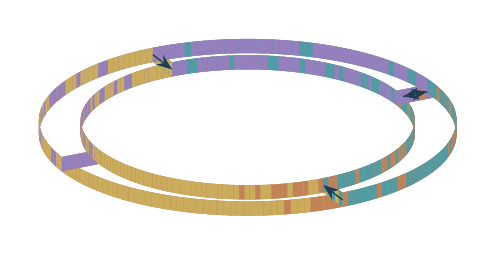
\begin{tikzpicture}[x=4.81857cm,y=4.81857cm]
\path[use as bounding box] (-0.579956,-0.262584) rectangle (0.579956,0.262584);
\path[fill=copper!82,draw=copper!82,line width=.08pt] (0.006956,-0.232584) -- (-0.011042,-0.232558) -- (-0.011042,-0.195716) -- (0.006956,-0.195742) -- cycle;
\path[fill=gold!82,draw=gold!82,line width=.08pt] (0.006956,-0.232584) -- (-0.011042,-0.232558) -- (-0.011042,-0.195716) -- (0.006956,-0.195742) -- cycle;
\path[fill=copper!82,draw=copper!82,line width=.08pt] (0.024946,-0.232381) -- (0.006956,-0.232584) -- (0.006956,-0.195742) -- (0.024946,-0.195538) -- cycle;
\path[fill=gold!82,draw=gold!82,line width=.08pt] (0.024946,-0.232381) -- (0.006956,-0.232584) -- (0.006956,-0.195742) -- (0.024946,-0.195538) -- cycle;
\path[fill=copper!82,draw=copper!82,line width=.08pt] (-0.011042,-0.232558) -- (-0.029028,-0.232303) -- (-0.029028,-0.195460) -- (-0.011042,-0.195716) -- cycle;
\path[fill=gold!82,draw=gold!82,line width=.08pt] (-0.011042,-0.232558) -- (-0.029028,-0.232303) -- (-0.029028,-0.195460) -- (-0.011042,-0.195716) -- cycle;
\path[fill=copper!82,draw=copper!82,line width=.08pt] (0.042910,-0.231948) -- (0.024946,-0.232381) -- (0.024946,-0.195538) -- (0.042910,-0.195106) -- cycle;
\path[fill=gold!82,draw=gold!82,line width=.08pt] (0.042910,-0.231948) -- (0.024946,-0.232381) -- (0.024946,-0.195538) -- (0.042910,-0.195106) -- cycle;
\path[fill=copper!82,draw=copper!82,line width=.08pt] (-0.029028,-0.232303) -- (-0.046983,-0.231818) -- (-0.046983,-0.194976) -- (-0.029028,-0.195460) -- cycle;
\path[fill=gold!82,draw=gold!82,line width=.08pt] (-0.029028,-0.232303) -- (-0.046983,-0.231818) -- (-0.046983,-0.194976) -- (-0.029028,-0.195460) -- cycle;
\path[fill=copper!82,draw=copper!82,line width=.08pt] (0.060828,-0.231287) -- (0.042910,-0.231948) -- (0.042910,-0.195106) -- (0.060828,-0.194445) -- cycle;
\path[fill=gold!82,draw=gold!82,line width=.08pt] (0.060828,-0.231287) -- (0.042910,-0.231948) -- (0.042910,-0.195106) -- (0.060828,-0.194445) -- cycle;
\path[fill=copper!82,draw=copper!82,line width=.08pt] (-0.046983,-0.231818) -- (-0.064887,-0.231106) -- (-0.064887,-0.194263) -- (-0.046983,-0.194976) -- cycle;
\path[fill=gold!82,draw=gold!82,line width=.08pt] (-0.046983,-0.231818) -- (-0.064887,-0.231106) -- (-0.064887,-0.194263) -- (-0.046983,-0.194976) -- cycle;
\path[fill=copper!82,draw=copper!82,line width=.08pt] (0.078680,-0.230398) -- (0.060828,-0.231287) -- (0.060828,-0.194445) -- (0.078680,-0.193556) -- cycle;
\path[fill=gold!82,draw=gold!82,line width=.08pt] (0.078680,-0.230398) -- (0.060828,-0.231287) -- (0.060828,-0.194445) -- (0.078680,-0.193556) -- cycle;
\path[fill=copper!82,draw=copper!82,line width=.08pt] (-0.064887,-0.231106) -- (-0.082722,-0.230165) -- (-0.082722,-0.193322) -- (-0.064887,-0.194263) -- cycle;
\path[fill=gold!82,draw=gold!82,line width=.08pt] (-0.064887,-0.231106) -- (-0.082722,-0.230165) -- (-0.082722,-0.193322) -- (-0.064887,-0.194263) -- cycle;
\path[fill=copper!82,draw=copper!82,line width=.08pt] (0.096448,-0.229282) -- (0.078680,-0.230398) -- (0.078680,-0.193556) -- (0.096448,-0.192440) -- cycle;
\path[fill=gold!82,draw=gold!82,line width=.08pt] (0.096448,-0.229282) -- (0.078680,-0.230398) -- (0.078680,-0.193556) -- (0.096448,-0.192440) -- cycle;
\path[fill=copper!82,draw=copper!82,line width=.08pt] (-0.082722,-0.230165) -- (-0.100469,-0.228998) -- (-0.100469,-0.192155) -- (-0.082722,-0.193322) -- cycle;
\path[fill=gold!82,draw=gold!82,line width=.08pt] (-0.082722,-0.230165) -- (-0.100469,-0.228998) -- (-0.100469,-0.192155) -- (-0.082722,-0.193322) -- cycle;
\path[fill=gold!82,draw=gold!82,line width=.08pt] (0.114113,-0.227941) -- (0.096448,-0.229282) -- (0.096448,-0.192440) -- (0.114113,-0.191098) -- cycle;
\path[fill=copper!82,draw=copper!82,line width=.08pt] (0.114113,-0.227941) -- (0.096448,-0.229282) -- (0.096448,-0.192440) -- (0.114113,-0.191098) -- cycle;
\path[fill=copper!82,draw=copper!82,line width=.08pt] (-0.100469,-0.228998) -- (-0.118108,-0.227605) -- (-0.118108,-0.190762) -- (-0.100469,-0.192155) -- cycle;
\path[fill=gold!82,draw=gold!82,line width=.08pt] (-0.100469,-0.228998) -- (-0.118108,-0.227605) -- (-0.118108,-0.190762) -- (-0.100469,-0.192155) -- cycle;
\path[fill=copper!82,draw=copper!82,line width=.08pt] (0.131656,-0.226375) -- (0.114113,-0.227941) -- (0.114113,-0.191098) -- (0.131656,-0.189532) -- cycle;
\path[fill=gold!82,draw=gold!82,line width=.08pt] (0.131656,-0.226375) -- (0.114113,-0.227941) -- (0.114113,-0.191098) -- (0.131656,-0.189532) -- cycle;
\path[fill=copper!82,draw=copper!82,line width=.08pt] (-0.118108,-0.227605) -- (-0.135620,-0.225988) -- (-0.135620,-0.189145) -- (-0.118108,-0.190762) -- cycle;
\path[fill=gold!82,draw=gold!82,line width=.08pt] (-0.118108,-0.227605) -- (-0.135620,-0.225988) -- (-0.135620,-0.189145) -- (-0.118108,-0.190762) -- cycle;
\path[fill=copper!82,draw=copper!82,line width=.08pt] (0.149058,-0.224586) -- (0.131656,-0.226375) -- (0.131656,-0.189532) -- (0.149058,-0.187743) -- cycle;
\path[fill=gold!82,draw=gold!82,line width=.08pt] (0.149058,-0.224586) -- (0.131656,-0.226375) -- (0.131656,-0.189532) -- (0.149058,-0.187743) -- cycle;
\path[fill=copper!82,draw=copper!82,line width=.08pt] (-0.135620,-0.225988) -- (-0.152987,-0.224149) -- (-0.152987,-0.187306) -- (-0.135620,-0.189145) -- cycle;
\path[fill=gold!82,draw=gold!82,line width=.08pt] (-0.135620,-0.225988) -- (-0.152987,-0.224149) -- (-0.152987,-0.187306) -- (-0.135620,-0.189145) -- cycle;
\path[fill=copper!82,draw=copper!82,line width=.08pt] (0.166300,-0.222576) -- (0.149058,-0.224586) -- (0.149058,-0.187743) -- (0.166300,-0.185734) -- cycle;
\path[fill=gold!82,draw=gold!82,line width=.08pt] (0.166300,-0.222576) -- (0.149058,-0.224586) -- (0.149058,-0.187743) -- (0.166300,-0.185734) -- cycle;
\path[fill=copper!82,draw=copper!82,line width=.08pt] (-0.152987,-0.224149) -- (-0.170191,-0.222089) -- (-0.170191,-0.185247) -- (-0.152987,-0.187306) -- cycle;
\path[fill=gold!82,draw=gold!82,line width=.08pt] (-0.152987,-0.224149) -- (-0.170191,-0.222089) -- (-0.170191,-0.185247) -- (-0.152987,-0.187306) -- cycle;
\path[fill=gold!82,draw=gold!82,line width=.08pt] (0.183364,-0.220348) -- (0.166300,-0.222576) -- (0.166300,-0.185734) -- (0.183364,-0.183505) -- cycle;
\path[fill=copper!82,draw=copper!82,line width=.08pt] (0.183364,-0.220348) -- (0.166300,-0.222576) -- (0.166300,-0.185734) -- (0.183364,-0.183505) -- cycle;
\path[fill=copper!82,draw=copper!82,line width=.08pt] (-0.170191,-0.222089) -- (-0.187212,-0.219812) -- (-0.187212,-0.182969) -- (-0.170191,-0.185247) -- cycle;
\path[fill=gold!82,draw=gold!82,line width=.08pt] (-0.170191,-0.222089) -- (-0.187212,-0.219812) -- (-0.187212,-0.182969) -- (-0.170191,-0.185247) -- cycle;
\path[fill=gold!82,draw=gold!82,line width=.08pt] (0.200232,-0.217903) -- (0.183364,-0.220348) -- (0.183364,-0.183505) -- (0.200232,-0.181061) -- cycle;
\path[fill=copper!82,draw=copper!82,line width=.08pt] (0.200232,-0.217903) -- (0.183364,-0.220348) -- (0.183364,-0.183505) -- (0.200232,-0.181061) -- cycle;
\path[fill=copper!82,draw=copper!82,line width=.08pt] (-0.187212,-0.219812) -- (-0.204033,-0.217319) -- (-0.204033,-0.180476) -- (-0.187212,-0.182969) -- cycle;
\path[fill=gold!82,draw=gold!82,line width=.08pt] (-0.187212,-0.219812) -- (-0.204033,-0.217319) -- (-0.204033,-0.180476) -- (-0.187212,-0.182969) -- cycle;
\path[fill=gold!82,draw=gold!82,line width=.08pt] (0.216885,-0.215245) -- (0.200232,-0.217903) -- (0.200232,-0.181061) -- (0.216885,-0.178403) -- cycle;
\path[fill=copper!82,draw=copper!82,line width=.08pt] (0.216885,-0.215245) -- (0.200232,-0.217903) -- (0.200232,-0.181061) -- (0.216885,-0.178403) -- cycle;
\path[fill=copper!82,draw=copper!82,line width=.08pt] (-0.204033,-0.217319) -- (-0.220635,-0.214612) -- (-0.220635,-0.177770) -- (-0.204033,-0.180476) -- cycle;
\path[fill=gold!82,draw=gold!82,line width=.08pt] (-0.204033,-0.217319) -- (-0.220635,-0.214612) -- (-0.220635,-0.177770) -- (-0.204033,-0.180476) -- cycle;
\path[fill=gold!82,draw=gold!82,line width=.08pt] (0.233307,-0.212377) -- (0.216885,-0.215245) -- (0.216885,-0.178403) -- (0.233307,-0.175534) -- cycle;
\path[fill=copper!82,draw=copper!82,line width=.08pt] (0.233307,-0.212377) -- (0.216885,-0.215245) -- (0.216885,-0.178403) -- (0.233307,-0.175534) -- cycle;
\path[fill=copper!82,draw=copper!82,line width=.08pt] (-0.220635,-0.214612) -- (-0.237001,-0.211696) -- (-0.237001,-0.174854) -- (-0.220635,-0.177770) -- cycle;
\path[fill=gold!82,draw=gold!82,line width=.08pt] (-0.220635,-0.214612) -- (-0.237001,-0.211696) -- (-0.237001,-0.174854) -- (-0.220635,-0.177770) -- cycle;
\path[fill=gold!82,draw=gold!82,line width=.08pt] (0.249478,-0.209300) -- (0.233307,-0.212377) -- (0.233307,-0.175534) -- (0.249478,-0.172458) -- cycle;
\path[fill=copper!82,draw=copper!82,line width=.08pt] (0.249478,-0.209300) -- (0.233307,-0.212377) -- (0.233307,-0.175534) -- (0.249478,-0.172458) -- cycle;
\path[fill=copper!82,draw=copper!82,line width=.08pt] (-0.237001,-0.211696) -- (-0.253113,-0.208573) -- (-0.253113,-0.171731) -- (-0.237001,-0.174854) -- cycle;
\path[fill=gold!82,draw=gold!82,line width=.08pt] (-0.237001,-0.211696) -- (-0.253113,-0.208573) -- (-0.253113,-0.171731) -- (-0.237001,-0.174854) -- cycle;
\path[fill=teal!82,draw=teal!82,line width=.08pt] (0.265382,-0.206019) -- (0.249478,-0.209300) -- (0.249478,-0.172458) -- (0.265382,-0.169177) -- cycle;
\path[fill=copper!82,draw=copper!82,line width=.08pt] (0.265382,-0.206019) -- (0.249478,-0.209300) -- (0.249478,-0.172458) -- (0.265382,-0.169177) -- cycle;
\path[fill=copper!82,draw=copper!82,line width=.08pt] (-0.253113,-0.208573) -- (-0.268954,-0.205246) -- (-0.268954,-0.168404) -- (-0.253113,-0.171731) -- cycle;
\path[fill=gold!82,draw=gold!82,line width=.08pt] (-0.253113,-0.208573) -- (-0.268954,-0.205246) -- (-0.268954,-0.168404) -- (-0.253113,-0.171731) -- cycle;
\path[fill=gold!82,draw=gold!82,line width=.08pt] (0.239499,-0.201665) -- (0.249478,-0.209300) -- (0.249478,-0.172458) -- (0.239499,-0.164822) -- cycle;
\path[fill=teal!82,draw=teal!82,line width=.08pt] (0.249478,-0.209300) -- (0.239499,-0.201665) -- (0.239499,-0.164822) -- (0.249478,-0.172458) -- cycle;
\path[fill=copper!82,draw=copper!82,line width=.08pt] (0.281002,-0.202537) -- (0.265382,-0.206019) -- (0.265382,-0.169177) -- (0.281002,-0.165695) -- cycle;
\path[fill=teal!82,draw=teal!82,line width=.08pt] (0.281002,-0.202537) -- (0.265382,-0.206019) -- (0.265382,-0.169177) -- (0.281002,-0.165695) -- cycle;
\path[fill=copper!82,draw=copper!82,line width=.08pt] (-0.268954,-0.205246) -- (-0.284507,-0.201719) -- (-0.284507,-0.164877) -- (-0.268954,-0.168404) -- cycle;
\path[fill=gold!82,draw=gold!82,line width=.08pt] (-0.268954,-0.205246) -- (-0.284507,-0.201719) -- (-0.284507,-0.164877) -- (-0.268954,-0.168404) -- cycle;
\path[fill=copper!82,draw=copper!82,line width=.08pt] (0.296321,-0.198858) -- (0.281002,-0.202537) -- (0.281002,-0.165695) -- (0.296321,-0.162016) -- cycle;
\path[fill=teal!82,draw=teal!82,line width=.08pt] (0.296321,-0.198858) -- (0.281002,-0.202537) -- (0.281002,-0.165695) -- (0.296321,-0.162016) -- cycle;
\path[fill=copper!82,draw=copper!82,line width=.08pt] (-0.284507,-0.201719) -- (-0.299756,-0.197996) -- (-0.299756,-0.161154) -- (-0.284507,-0.164877) -- cycle;
\path[fill=gold!82,draw=gold!82,line width=.08pt] (-0.284507,-0.201719) -- (-0.299756,-0.197996) -- (-0.299756,-0.161154) -- (-0.284507,-0.164877) -- cycle;
\path[fill=teal!82,draw=teal!82,line width=.08pt] (0.239499,-0.201665) -- (0.229520,-0.194030) -- (0.229520,-0.157187) -- (0.239499,-0.164822) -- cycle;
\path[fill=gold!82,draw=gold!82,line width=.08pt] (0.229520,-0.194030) -- (0.239499,-0.201665) -- (0.239499,-0.164822) -- (0.229520,-0.157187) -- cycle;
\path[fill=copper!82,draw=copper!82,line width=.08pt] (0.311323,-0.194986) -- (0.296321,-0.198858) -- (0.296321,-0.162016) -- (0.311323,-0.158144) -- cycle;
\path[fill=teal!82,draw=teal!82,line width=.08pt] (0.311323,-0.194986) -- (0.296321,-0.198858) -- (0.296321,-0.162016) -- (0.311323,-0.158144) -- cycle;
\path[fill=copper!82,draw=copper!82,line width=.08pt] (-0.299756,-0.197996) -- (-0.314683,-0.194081) -- (-0.314683,-0.157238) -- (-0.299756,-0.161154) -- cycle;
\path[fill=gold!82,draw=gold!82,line width=.08pt] (-0.299756,-0.197996) -- (-0.314683,-0.194081) -- (-0.314683,-0.157238) -- (-0.299756,-0.161154) -- cycle;
\path[fill=copper!82,draw=copper!82,line width=.08pt] (0.325991,-0.190925) -- (0.311323,-0.194986) -- (0.311323,-0.158144) -- (0.325991,-0.154083) -- cycle;
\path[fill=teal!82,draw=teal!82,line width=.08pt] (0.325991,-0.190925) -- (0.311323,-0.194986) -- (0.311323,-0.158144) -- (0.325991,-0.154083) -- cycle;
\path[fill=copper!82,draw=copper!82,line width=.08pt] (-0.314683,-0.194081) -- (-0.329274,-0.189977) -- (-0.329274,-0.153135) -- (-0.314683,-0.157238) -- cycle;
\path[fill=gold!82,draw=gold!82,line width=.08pt] (-0.314683,-0.194081) -- (-0.329274,-0.189977) -- (-0.329274,-0.153135) -- (-0.314683,-0.157238) -- cycle;
\path[fill=gold!82,draw=gold!82,line width=.08pt] (0.219541,-0.186395) -- (0.229520,-0.194030) -- (0.229520,-0.157187) -- (0.219541,-0.149552) -- cycle;
\path[fill=teal!82,draw=teal!82,line width=.08pt] (0.229520,-0.194030) -- (0.219541,-0.186395) -- (0.219541,-0.149552) -- (0.229520,-0.157187) -- cycle;
\path[fill=copper!82,draw=copper!82,line width=.08pt] (-0.008834,-0.189731) -- (0.005565,-0.189752) -- (0.005565,-0.152909) -- (-0.008834,-0.152888) -- cycle;
\path[fill=gold!82,draw=gold!82,line width=.08pt] (-0.008834,-0.189731) -- (0.005565,-0.189752) -- (0.005565,-0.152909) -- (-0.008834,-0.152888) -- cycle;
\path[fill=copper!82,draw=copper!82,line width=.08pt] (0.005565,-0.189752) -- (0.019957,-0.189589) -- (0.019957,-0.152747) -- (0.005565,-0.152909) -- cycle;
\path[fill=gold!82,draw=gold!82,line width=.08pt] (0.005565,-0.189752) -- (0.019957,-0.189589) -- (0.019957,-0.152747) -- (0.005565,-0.152909) -- cycle;
\path[fill=gold!82,draw=gold!82,line width=.08pt] (-0.023222,-0.189526) -- (-0.008834,-0.189731) -- (-0.008834,-0.152888) -- (-0.023222,-0.152684) -- cycle;
\path[fill=copper!82,draw=copper!82,line width=.08pt] (-0.023222,-0.189526) -- (-0.008834,-0.189731) -- (-0.008834,-0.152888) -- (-0.023222,-0.152684) -- cycle;
\path[fill=gold!82,draw=gold!82,line width=.08pt] (0.019957,-0.189589) -- (0.034328,-0.189243) -- (0.034328,-0.152401) -- (0.019957,-0.152747) -- cycle;
\path[fill=copper!82,draw=copper!82,line width=.08pt] (0.019957,-0.189589) -- (0.034328,-0.189243) -- (0.034328,-0.152401) -- (0.019957,-0.152747) -- cycle;
\path[fill=copper!82,draw=copper!82,line width=.08pt] (-0.037586,-0.189139) -- (-0.023222,-0.189526) -- (-0.023222,-0.152684) -- (-0.037586,-0.152297) -- cycle;
\path[fill=gold!82,draw=gold!82,line width=.08pt] (-0.037586,-0.189139) -- (-0.023222,-0.189526) -- (-0.023222,-0.152684) -- (-0.037586,-0.152297) -- cycle;
\path[fill=copper!82,draw=copper!82,line width=.08pt] (0.034328,-0.189243) -- (0.048662,-0.188714) -- (0.048662,-0.151872) -- (0.034328,-0.152401) -- cycle;
\path[fill=gold!82,draw=gold!82,line width=.08pt] (0.034328,-0.189243) -- (0.048662,-0.188714) -- (0.048662,-0.151872) -- (0.034328,-0.152401) -- cycle;
\path[fill=copper!82,draw=copper!82,line width=.08pt] (-0.051910,-0.188569) -- (-0.037586,-0.189139) -- (-0.037586,-0.152297) -- (-0.051910,-0.151726) -- cycle;
\path[fill=gold!82,draw=gold!82,line width=.08pt] (-0.051910,-0.188569) -- (-0.037586,-0.189139) -- (-0.037586,-0.152297) -- (-0.051910,-0.151726) -- cycle;
\path[fill=copper!82,draw=copper!82,line width=.08pt] (0.340310,-0.186679) -- (0.325991,-0.190925) -- (0.325991,-0.154083) -- (0.340310,-0.149837) -- cycle;
\path[fill=teal!82,draw=teal!82,line width=.08pt] (0.340310,-0.186679) -- (0.325991,-0.190925) -- (0.325991,-0.154083) -- (0.340310,-0.149837) -- cycle;
\path[fill=copper!82,draw=copper!82,line width=.08pt] (0.048662,-0.188714) -- (0.062944,-0.188003) -- (0.062944,-0.151161) -- (0.048662,-0.151872) -- cycle;
\path[fill=gold!82,draw=gold!82,line width=.08pt] (0.048662,-0.188714) -- (0.062944,-0.188003) -- (0.062944,-0.151161) -- (0.048662,-0.151872) -- cycle;
\path[fill=copper!82,draw=copper!82,line width=.08pt] (-0.066178,-0.187816) -- (-0.051910,-0.188569) -- (-0.051910,-0.151726) -- (-0.066178,-0.150974) -- cycle;
\path[fill=gold!82,draw=gold!82,line width=.08pt] (-0.066178,-0.187816) -- (-0.051910,-0.188569) -- (-0.051910,-0.151726) -- (-0.066178,-0.150974) -- cycle;
\path[fill=copper!82,draw=copper!82,line width=.08pt] (-0.329274,-0.189977) -- (-0.343511,-0.185690) -- (-0.343511,-0.148847) -- (-0.329274,-0.153135) -- cycle;
\path[fill=gold!82,draw=gold!82,line width=.08pt] (-0.329274,-0.189977) -- (-0.343511,-0.185690) -- (-0.343511,-0.148847) -- (-0.329274,-0.153135) -- cycle;
\path[fill=gold!82,draw=gold!82,line width=.08pt] (0.062944,-0.188003) -- (0.077159,-0.187110) -- (0.077159,-0.150268) -- (0.062944,-0.151161) -- cycle;
\path[fill=copper!82,draw=copper!82,line width=.08pt] (0.062944,-0.188003) -- (0.077159,-0.187110) -- (0.077159,-0.150268) -- (0.062944,-0.151161) -- cycle;
\path[fill=copper!82,draw=copper!82,line width=.08pt] (-0.080375,-0.186882) -- (-0.066178,-0.187816) -- (-0.066178,-0.150974) -- (-0.080375,-0.150040) -- cycle;
\path[fill=gold!82,draw=gold!82,line width=.08pt] (-0.080375,-0.186882) -- (-0.066178,-0.187816) -- (-0.066178,-0.150974) -- (-0.080375,-0.150040) -- cycle;
\path[fill=gold!82,draw=gold!82,line width=.08pt] (0.077159,-0.187110) -- (0.091291,-0.186037) -- (0.091291,-0.149194) -- (0.077159,-0.150268) -- cycle;
\path[fill=copper!82,draw=copper!82,line width=.08pt] (0.077159,-0.187110) -- (0.091291,-0.186037) -- (0.091291,-0.149194) -- (0.077159,-0.150268) -- cycle;
\path[fill=copper!82,draw=copper!82,line width=.08pt] (-0.094486,-0.185768) -- (-0.080375,-0.186882) -- (-0.080375,-0.150040) -- (-0.094486,-0.148926) -- cycle;
\path[fill=gold!82,draw=gold!82,line width=.08pt] (-0.094486,-0.185768) -- (-0.080375,-0.186882) -- (-0.080375,-0.150040) -- (-0.094486,-0.148926) -- cycle;
\path[fill=gold!82,draw=gold!82,line width=.08pt] (0.091291,-0.186037) -- (0.105325,-0.184784) -- (0.105325,-0.147941) -- (0.091291,-0.149194) -- cycle;
\path[fill=copper!82,draw=copper!82,line width=.08pt] (0.091291,-0.186037) -- (0.105325,-0.184784) -- (0.105325,-0.147941) -- (0.091291,-0.149194) -- cycle;
\path[fill=copper!82,draw=copper!82,line width=.08pt] (-0.108496,-0.184475) -- (-0.094486,-0.185768) -- (-0.094486,-0.148926) -- (-0.108496,-0.147632) -- cycle;
\path[fill=gold!82,draw=gold!82,line width=.08pt] (-0.108496,-0.184475) -- (-0.094486,-0.185768) -- (-0.094486,-0.148926) -- (-0.108496,-0.147632) -- cycle;
\path[fill=teal!82,draw=teal!82,line width=.08pt] (0.354265,-0.182253) -- (0.340310,-0.186679) -- (0.340310,-0.149837) -- (0.354265,-0.145411) -- cycle;
\path[fill=copper!82,draw=copper!82,line width=.08pt] (0.354265,-0.182253) -- (0.340310,-0.186679) -- (0.340310,-0.149837) -- (0.354265,-0.145411) -- cycle;
\path[fill=copper!82,draw=copper!82,line width=.08pt] (0.105325,-0.184784) -- (0.119246,-0.183353) -- (0.119246,-0.146510) -- (0.105325,-0.147941) -- cycle;
\path[fill=gold!82,draw=gold!82,line width=.08pt] (0.105325,-0.184784) -- (0.119246,-0.183353) -- (0.119246,-0.146510) -- (0.105325,-0.147941) -- cycle;
\path[fill=copper!82,draw=copper!82,line width=.08pt] (-0.122390,-0.183003) -- (-0.108496,-0.184475) -- (-0.108496,-0.147632) -- (-0.122390,-0.146161) -- cycle;
\path[fill=gold!82,draw=gold!82,line width=.08pt] (-0.122390,-0.183003) -- (-0.108496,-0.184475) -- (-0.108496,-0.147632) -- (-0.122390,-0.146161) -- cycle;
\path[fill=copper!82,draw=copper!82,line width=.08pt] (-0.343511,-0.185690) -- (-0.357381,-0.181223) -- (-0.357381,-0.144381) -- (-0.343511,-0.148847) -- cycle;
\path[fill=gold!82,draw=gold!82,line width=.08pt] (-0.343511,-0.185690) -- (-0.357381,-0.181223) -- (-0.357381,-0.144381) -- (-0.343511,-0.148847) -- cycle;
\path[fill=gold!82,draw=gold!82,line width=.08pt] (0.209561,-0.178759) -- (0.219541,-0.186395) -- (0.219541,-0.149552) -- (0.209561,-0.141917) -- cycle;
\path[fill=teal!82,draw=teal!82,line width=.08pt] (0.219541,-0.186395) -- (0.209561,-0.178759) -- (0.209561,-0.141917) -- (0.219541,-0.149552) -- cycle;
\path[fill=gold!82,draw=gold!82,line width=.08pt] (0.119246,-0.183353) -- (0.133040,-0.181745) -- (0.133040,-0.144903) -- (0.119246,-0.146510) -- cycle;
\path[fill=copper!82,draw=copper!82,line width=.08pt] (0.119246,-0.183353) -- (0.133040,-0.181745) -- (0.133040,-0.144903) -- (0.119246,-0.146510) -- cycle;
\path[fill=copper!82,draw=copper!82,line width=.08pt] (-0.136153,-0.181356) -- (-0.122390,-0.183003) -- (-0.122390,-0.146161) -- (-0.136153,-0.144513) -- cycle;
\path[fill=gold!82,draw=gold!82,line width=.08pt] (-0.136153,-0.181356) -- (-0.122390,-0.183003) -- (-0.122390,-0.146161) -- (-0.136153,-0.144513) -- cycle;
\path[fill=gold!82,draw=gold!82,line width=.08pt] (0.133040,-0.181745) -- (0.146691,-0.179963) -- (0.146691,-0.143120) -- (0.133040,-0.144903) -- cycle;
\path[fill=copper!82,draw=copper!82,line width=.08pt] (0.133040,-0.181745) -- (0.146691,-0.179963) -- (0.146691,-0.143120) -- (0.133040,-0.144903) -- cycle;
\path[fill=copper!82,draw=copper!82,line width=.08pt] (-0.149770,-0.179534) -- (-0.136153,-0.181356) -- (-0.136153,-0.144513) -- (-0.149770,-0.142691) -- cycle;
\path[fill=gold!82,draw=gold!82,line width=.08pt] (-0.149770,-0.179534) -- (-0.136153,-0.181356) -- (-0.136153,-0.144513) -- (-0.149770,-0.142691) -- cycle;
\path[fill=copper!82,draw=copper!82,line width=.08pt] (0.367841,-0.177651) -- (0.354265,-0.182253) -- (0.354265,-0.145411) -- (0.367841,-0.140809) -- cycle;
\path[fill=teal!82,draw=teal!82,line width=.08pt] (0.367841,-0.177651) -- (0.354265,-0.182253) -- (0.354265,-0.145411) -- (0.367841,-0.140809) -- cycle;
\path[fill=gold!82,draw=gold!82,line width=.08pt] (0.146691,-0.179963) -- (0.160186,-0.178007) -- (0.160186,-0.141165) -- (0.146691,-0.143120) -- cycle;
\path[fill=copper!82,draw=copper!82,line width=.08pt] (0.146691,-0.179963) -- (0.160186,-0.178007) -- (0.160186,-0.141165) -- (0.146691,-0.143120) -- cycle;
\path[fill=copper!82,draw=copper!82,line width=.08pt] (-0.357381,-0.181223) -- (-0.370869,-0.176583) -- (-0.370869,-0.139740) -- (-0.357381,-0.144381) -- cycle;
\path[fill=gold!82,draw=gold!82,line width=.08pt] (-0.357381,-0.181223) -- (-0.370869,-0.176583) -- (-0.370869,-0.139740) -- (-0.357381,-0.144381) -- cycle;
\path[fill=copper!82,draw=copper!82,line width=.08pt] (-0.163226,-0.177539) -- (-0.149770,-0.179534) -- (-0.149770,-0.142691) -- (-0.163226,-0.140697) -- cycle;
\path[fill=gold!82,draw=gold!82,line width=.08pt] (-0.163226,-0.177539) -- (-0.149770,-0.179534) -- (-0.149770,-0.142691) -- (-0.163226,-0.140697) -- cycle;
\path[fill=copper!82,draw=copper!82,line width=.08pt] (0.160186,-0.178007) -- (0.173508,-0.175881) -- (0.173508,-0.139038) -- (0.160186,-0.141165) -- cycle;
\path[fill=gold!82,draw=gold!82,line width=.08pt] (0.160186,-0.178007) -- (0.173508,-0.175881) -- (0.173508,-0.139038) -- (0.160186,-0.141165) -- cycle;
\path[fill=copper!82,draw=copper!82,line width=.08pt] (-0.176508,-0.175374) -- (-0.163226,-0.177539) -- (-0.163226,-0.140697) -- (-0.176508,-0.138532) -- cycle;
\path[fill=gold!82,draw=gold!82,line width=.08pt] (-0.176508,-0.175374) -- (-0.163226,-0.177539) -- (-0.163226,-0.140697) -- (-0.176508,-0.138532) -- cycle;
\path[fill=copper!82,draw=copper!82,line width=.08pt] (0.381023,-0.172879) -- (0.367841,-0.177651) -- (0.367841,-0.140809) -- (0.381023,-0.136037) -- cycle;
\path[fill=teal!82,draw=teal!82,line width=.08pt] (0.381023,-0.172879) -- (0.367841,-0.177651) -- (0.367841,-0.140809) -- (0.381023,-0.136037) -- cycle;
\path[fill=teal!82,draw=teal!82,line width=.08pt] (0.209561,-0.178759) -- (0.199582,-0.171124) -- (0.199582,-0.134282) -- (0.209561,-0.141917) -- cycle;
\path[fill=gold!82,draw=gold!82,line width=.08pt] (0.199582,-0.171124) -- (0.209561,-0.178759) -- (0.209561,-0.141917) -- (0.199582,-0.134282) -- cycle;
\path[fill=copper!82,draw=copper!82,line width=.08pt] (0.173508,-0.175881) -- (0.186645,-0.173586) -- (0.186645,-0.136743) -- (0.173508,-0.139038) -- cycle;
\path[fill=gold!82,draw=gold!82,line width=.08pt] (0.173508,-0.175881) -- (0.186645,-0.173586) -- (0.186645,-0.136743) -- (0.173508,-0.139038) -- cycle;
\path[fill=copper!82,draw=copper!82,line width=.08pt] (-0.189601,-0.173041) -- (-0.176508,-0.175374) -- (-0.176508,-0.138532) -- (-0.189601,-0.136199) -- cycle;
\path[fill=gold!82,draw=gold!82,line width=.08pt] (-0.189601,-0.173041) -- (-0.176508,-0.175374) -- (-0.176508,-0.138532) -- (-0.189601,-0.136199) -- cycle;
\path[fill=copper!82,draw=copper!82,line width=.08pt] (-0.370869,-0.176583) -- (-0.383959,-0.171773) -- (-0.383959,-0.134930) -- (-0.370869,-0.139740) -- cycle;
\path[fill=gold!82,draw=gold!82,line width=.08pt] (-0.370869,-0.176583) -- (-0.383959,-0.171773) -- (-0.383959,-0.134930) -- (-0.370869,-0.139740) -- cycle;
\path[fill=gold!82,draw=gold!82,line width=.08pt] (0.186645,-0.173586) -- (0.199582,-0.171124) -- (0.199582,-0.134282) -- (0.186645,-0.136743) -- cycle;
\path[fill=copper!82,draw=copper!82,line width=.08pt] (0.186645,-0.173586) -- (0.199582,-0.171124) -- (0.199582,-0.134282) -- (0.186645,-0.136743) -- cycle;
\path[fill=copper!82,draw=copper!82,line width=.08pt] (-0.202490,-0.170543) -- (-0.189601,-0.173041) -- (-0.189601,-0.136199) -- (-0.202490,-0.133700) -- cycle;
\path[fill=gold!82,draw=gold!82,line width=.08pt] (-0.202490,-0.170543) -- (-0.189601,-0.173041) -- (-0.189601,-0.136199) -- (-0.202490,-0.133700) -- cycle;
\path[fill=copper!82,draw=copper!82,line width=.08pt] (0.393796,-0.167942) -- (0.381023,-0.172879) -- (0.381023,-0.136037) -- (0.393796,-0.131099) -- cycle;
\path[fill=teal!82,draw=teal!82,line width=.08pt] (0.393796,-0.167942) -- (0.381023,-0.172879) -- (0.381023,-0.136037) -- (0.393796,-0.131099) -- cycle;
\path[fill=copper!82,draw=copper!82,line width=.08pt] (0.199582,-0.171124) -- (0.212306,-0.168500) -- (0.212306,-0.131657) -- (0.199582,-0.134282) -- cycle;
\path[fill=teal!82,draw=teal!82,line width=.08pt] (0.199582,-0.171124) -- (0.212306,-0.168500) -- (0.212306,-0.131657) -- (0.199582,-0.134282) -- cycle;
\path[fill=copper!82,draw=copper!82,line width=.08pt] (-0.383959,-0.171773) -- (-0.396638,-0.166798) -- (-0.396638,-0.129956) -- (-0.383959,-0.134930) -- cycle;
\path[fill=gold!82,draw=gold!82,line width=.08pt] (-0.383959,-0.171773) -- (-0.396638,-0.166798) -- (-0.396638,-0.129956) -- (-0.383959,-0.134930) -- cycle;
\path[fill=copper!82,draw=copper!82,line width=.08pt] (-0.215163,-0.167881) -- (-0.202490,-0.170543) -- (-0.202490,-0.133700) -- (-0.215163,-0.131039) -- cycle;
\path[fill=gold!82,draw=gold!82,line width=.08pt] (-0.215163,-0.167881) -- (-0.202490,-0.170543) -- (-0.202490,-0.133700) -- (-0.215163,-0.131039) -- cycle;
\path[fill=teal!82,draw=teal!82,line width=.08pt] (0.212306,-0.168500) -- (0.224802,-0.165714) -- (0.224802,-0.128872) -- (0.212306,-0.131657) -- cycle;
\path[fill=copper!82,draw=copper!82,line width=.08pt] (0.212306,-0.168500) -- (0.224802,-0.165714) -- (0.224802,-0.128872) -- (0.212306,-0.131657) -- cycle;
\path[fill=copper!82,draw=copper!82,line width=.08pt] (-0.227606,-0.165060) -- (-0.215163,-0.167881) -- (-0.215163,-0.131039) -- (-0.227606,-0.128217) -- cycle;
\path[fill=gold!82,draw=gold!82,line width=.08pt] (-0.227606,-0.165060) -- (-0.215163,-0.167881) -- (-0.215163,-0.131039) -- (-0.227606,-0.128217) -- cycle;
\path[fill=teal!82,draw=teal!82,line width=.08pt] (0.406148,-0.162844) -- (0.393796,-0.167942) -- (0.393796,-0.131099) -- (0.406148,-0.126002) -- cycle;
\path[fill=copper!82,draw=copper!82,line width=.08pt] (0.406148,-0.162844) -- (0.393796,-0.167942) -- (0.393796,-0.131099) -- (0.406148,-0.126002) -- cycle;
\path[fill=teal!82,draw=teal!82,line width=.08pt] (0.224802,-0.165714) -- (0.237057,-0.162771) -- (0.237057,-0.125929) -- (0.224802,-0.128872) -- cycle;
\path[fill=copper!82,draw=copper!82,line width=.08pt] (0.224802,-0.165714) -- (0.237057,-0.162771) -- (0.237057,-0.125929) -- (0.224802,-0.128872) -- cycle;
\path[fill=copper!82,draw=copper!82,line width=.08pt] (-0.396638,-0.166798) -- (-0.408892,-0.161665) -- (-0.408892,-0.124823) -- (-0.396638,-0.129956) -- cycle;
\path[fill=gold!82,draw=gold!82,line width=.08pt] (-0.396638,-0.166798) -- (-0.408892,-0.161665) -- (-0.408892,-0.124823) -- (-0.396638,-0.129956) -- cycle;
\path[fill=copper!82,draw=copper!82,line width=.08pt] (-0.239804,-0.162081) -- (-0.227606,-0.165060) -- (-0.227606,-0.128217) -- (-0.239804,-0.125239) -- cycle;
\path[fill=gold!82,draw=gold!82,line width=.08pt] (-0.239804,-0.162081) -- (-0.227606,-0.165060) -- (-0.227606,-0.128217) -- (-0.239804,-0.125239) -- cycle;
\path[fill=copper!82,draw=copper!82,line width=.08pt] (0.237057,-0.162771) -- (0.249058,-0.159673) -- (0.249058,-0.122831) -- (0.237057,-0.125929) -- cycle;
\path[fill=teal!82,draw=teal!82,line width=.08pt] (0.237057,-0.162771) -- (0.249058,-0.159673) -- (0.249058,-0.122831) -- (0.237057,-0.125929) -- cycle;
\path[fill=copper!82,draw=copper!82,line width=.08pt] (-0.251746,-0.158949) -- (-0.239804,-0.162081) -- (-0.239804,-0.125239) -- (-0.251746,-0.122106) -- cycle;
\path[fill=gold!82,draw=gold!82,line width=.08pt] (-0.251746,-0.158949) -- (-0.239804,-0.162081) -- (-0.239804,-0.125239) -- (-0.251746,-0.122106) -- cycle;
\path[fill=teal!82,draw=teal!82,line width=.08pt] (0.418065,-0.157592) -- (0.406148,-0.162844) -- (0.406148,-0.126002) -- (0.418065,-0.120750) -- cycle;
\path[fill=copper!82,draw=copper!82,line width=.08pt] (0.418065,-0.157592) -- (0.406148,-0.162844) -- (0.406148,-0.126002) -- (0.418065,-0.120750) -- cycle;
\path[fill=copper!82,draw=copper!82,line width=.08pt] (-0.408892,-0.161665) -- (-0.420709,-0.156379) -- (-0.420709,-0.119536) -- (-0.408892,-0.124823) -- cycle;
\path[fill=gold!82,draw=gold!82,line width=.08pt] (-0.408892,-0.161665) -- (-0.420709,-0.156379) -- (-0.420709,-0.119536) -- (-0.408892,-0.124823) -- cycle;
\path[fill=copper!82,draw=copper!82,line width=.08pt] (0.249058,-0.159673) -- (0.260793,-0.156424) -- (0.260793,-0.119582) -- (0.249058,-0.122831) -- cycle;
\path[fill=teal!82,draw=teal!82,line width=.08pt] (0.249058,-0.159673) -- (0.260793,-0.156424) -- (0.260793,-0.119582) -- (0.249058,-0.122831) -- cycle;
\path[fill=copper!82,draw=copper!82,line width=.08pt] (-0.263419,-0.155666) -- (-0.251746,-0.158949) -- (-0.251746,-0.122106) -- (-0.263419,-0.118823) -- cycle;
\path[fill=gold!82,draw=gold!82,line width=.08pt] (-0.263419,-0.155666) -- (-0.251746,-0.158949) -- (-0.251746,-0.122106) -- (-0.263419,-0.118823) -- cycle;
\path[fill=copper!82,draw=copper!82,line width=.08pt] (0.429535,-0.152191) -- (0.418065,-0.157592) -- (0.418065,-0.120750) -- (0.429535,-0.115348) -- cycle;
\path[fill=teal!82,draw=teal!82,line width=.08pt] (0.429535,-0.152191) -- (0.418065,-0.157592) -- (0.418065,-0.120750) -- (0.429535,-0.115348) -- cycle;
\path[fill=copper!82,draw=copper!82,line width=.08pt] (0.260793,-0.156424) -- (0.272248,-0.153028) -- (0.272248,-0.116185) -- (0.260793,-0.119582) -- cycle;
\path[fill=teal!82,draw=teal!82,line width=.08pt] (0.260793,-0.156424) -- (0.272248,-0.153028) -- (0.272248,-0.116185) -- (0.260793,-0.119582) -- cycle;
\path[fill=copper!82,draw=copper!82,line width=.08pt] (-0.274809,-0.152236) -- (-0.263419,-0.155666) -- (-0.263419,-0.118823) -- (-0.274809,-0.115394) -- cycle;
\path[fill=gold!82,draw=gold!82,line width=.08pt] (-0.274809,-0.152236) -- (-0.263419,-0.155666) -- (-0.263419,-0.118823) -- (-0.274809,-0.115394) -- cycle;
\path[fill=copper!82,draw=copper!82,line width=.08pt] (-0.420709,-0.156379) -- (-0.432075,-0.150944) -- (-0.432075,-0.114102) -- (-0.420709,-0.119536) -- cycle;
\path[fill=gold!82,draw=gold!82,line width=.08pt] (-0.420709,-0.156379) -- (-0.432075,-0.150944) -- (-0.432075,-0.114102) -- (-0.420709,-0.119536) -- cycle;
\path[fill=copper!82,draw=copper!82,line width=.08pt] (0.272248,-0.153028) -- (0.283412,-0.149487) -- (0.283412,-0.112644) -- (0.272248,-0.116185) -- cycle;
\path[fill=teal!82,draw=teal!82,line width=.08pt] (0.272248,-0.153028) -- (0.283412,-0.149487) -- (0.283412,-0.112644) -- (0.272248,-0.116185) -- cycle;
\path[fill=copper!82,draw=copper!82,line width=.08pt] (-0.285905,-0.148663) -- (-0.274809,-0.152236) -- (-0.274809,-0.115394) -- (-0.285905,-0.111821) -- cycle;
\path[fill=gold!82,draw=gold!82,line width=.08pt] (-0.285905,-0.148663) -- (-0.274809,-0.152236) -- (-0.274809,-0.115394) -- (-0.285905,-0.111821) -- cycle;
\path[fill=copper!82,draw=copper!82,line width=.08pt] (0.440544,-0.146646) -- (0.429535,-0.152191) -- (0.429535,-0.115348) -- (0.440544,-0.109804) -- cycle;
\path[fill=teal!82,draw=teal!82,line width=.08pt] (0.440544,-0.146646) -- (0.429535,-0.152191) -- (0.429535,-0.115348) -- (0.440544,-0.109804) -- cycle;
\path[fill=copper!82,draw=copper!82,line width=.08pt] (-0.432075,-0.150944) -- (-0.442978,-0.145368) -- (-0.442978,-0.108526) -- (-0.432075,-0.114102) -- cycle;
\path[fill=gold!82,draw=gold!82,line width=.08pt] (-0.432075,-0.150944) -- (-0.442978,-0.145368) -- (-0.442978,-0.108526) -- (-0.432075,-0.114102) -- cycle;
\path[fill=teal!82,draw=teal!82,line width=.08pt] (0.283412,-0.149487) -- (0.294273,-0.145805) -- (0.294273,-0.108963) -- (0.283412,-0.112644) -- cycle;
\path[fill=copper!82,draw=copper!82,line width=.08pt] (0.283412,-0.149487) -- (0.294273,-0.145805) -- (0.294273,-0.108963) -- (0.283412,-0.112644) -- cycle;
\path[fill=copper!82,draw=copper!82,line width=.08pt] (-0.296695,-0.144950) -- (-0.285905,-0.148663) -- (-0.285905,-0.111821) -- (-0.296695,-0.108108) -- cycle;
\path[fill=gold!82,draw=gold!82,line width=.08pt] (-0.296695,-0.144950) -- (-0.285905,-0.148663) -- (-0.285905,-0.111821) -- (-0.296695,-0.108108) -- cycle;
\path[fill=copper!82,draw=copper!82,line width=.08pt] (0.294273,-0.145805) -- (0.304818,-0.141988) -- (0.304818,-0.105145) -- (0.294273,-0.108963) -- cycle;
\path[fill=teal!82,draw=teal!82,line width=.08pt] (0.294273,-0.145805) -- (0.304818,-0.141988) -- (0.304818,-0.105145) -- (0.294273,-0.108963) -- cycle;
\path[fill=copper!82,draw=copper!82,line width=.08pt] (0.451082,-0.140965) -- (0.440544,-0.146646) -- (0.440544,-0.109804) -- (0.451082,-0.104122) -- cycle;
\path[fill=teal!82,draw=teal!82,line width=.08pt] (0.451082,-0.140965) -- (0.440544,-0.146646) -- (0.440544,-0.109804) -- (0.451082,-0.104122) -- cycle;
\path[fill=copper!82,draw=copper!82,line width=.08pt] (-0.307167,-0.141102) -- (-0.296695,-0.144950) -- (-0.296695,-0.108108) -- (-0.307167,-0.104260) -- cycle;
\path[fill=gold!82,draw=gold!82,line width=.08pt] (-0.307167,-0.141102) -- (-0.296695,-0.144950) -- (-0.296695,-0.108108) -- (-0.307167,-0.104260) -- cycle;
\path[fill=copper!82,draw=copper!82,line width=.08pt] (-0.442978,-0.145368) -- (-0.453407,-0.139656) -- (-0.453407,-0.102814) -- (-0.442978,-0.108526) -- cycle;
\path[fill=gold!82,draw=gold!82,line width=.08pt] (-0.442978,-0.145368) -- (-0.453407,-0.139656) -- (-0.453407,-0.102814) -- (-0.442978,-0.108526) -- cycle;
\path[fill=copper!82,draw=copper!82,line width=.08pt] (0.304818,-0.141988) -- (0.315037,-0.138038) -- (0.315037,-0.101195) -- (0.304818,-0.105145) -- cycle;
\path[fill=teal!82,draw=teal!82,line width=.08pt] (0.304818,-0.141988) -- (0.315037,-0.138038) -- (0.315037,-0.101195) -- (0.304818,-0.105145) -- cycle;
\path[fill=copper!82,draw=copper!82,line width=.08pt] (-0.317311,-0.137123) -- (-0.307167,-0.141102) -- (-0.307167,-0.104260) -- (-0.317311,-0.100281) -- cycle;
\path[fill=gold!82,draw=gold!82,line width=.08pt] (-0.317311,-0.137123) -- (-0.307167,-0.141102) -- (-0.307167,-0.104260) -- (-0.317311,-0.100281) -- cycle;
\path[fill=copper!82,draw=copper!82,line width=.08pt] (0.461136,-0.135152) -- (0.451082,-0.140965) -- (0.451082,-0.104122) -- (0.461136,-0.098309) -- cycle;
\path[fill=teal!82,draw=teal!82,line width=.08pt] (0.461136,-0.135152) -- (0.451082,-0.140965) -- (0.451082,-0.104122) -- (0.461136,-0.098309) -- cycle;
\path[fill=copper!82,draw=copper!82,line width=.08pt] (-0.453407,-0.139656) -- (-0.463351,-0.133814) -- (-0.463351,-0.096972) -- (-0.453407,-0.102814) -- cycle;
\path[fill=gold!82,draw=gold!82,line width=.08pt] (-0.453407,-0.139656) -- (-0.463351,-0.133814) -- (-0.463351,-0.096972) -- (-0.453407,-0.102814) -- cycle;
\path[fill=copper!82,draw=copper!82,line width=.08pt] (0.315037,-0.138038) -- (0.324918,-0.133960) -- (0.324918,-0.097117) -- (0.315037,-0.101195) -- cycle;
\path[fill=teal!82,draw=teal!82,line width=.08pt] (0.315037,-0.138038) -- (0.324918,-0.133960) -- (0.324918,-0.097117) -- (0.315037,-0.101195) -- cycle;
\path[fill=copper!82,draw=copper!82,line width=.08pt] (-0.327114,-0.133016) -- (-0.317311,-0.137123) -- (-0.317311,-0.100281) -- (-0.327114,-0.096174) -- cycle;
\path[fill=gold!82,draw=gold!82,line width=.08pt] (-0.327114,-0.133016) -- (-0.317311,-0.137123) -- (-0.317311,-0.100281) -- (-0.327114,-0.096174) -- cycle;
\path[fill=copper!82,draw=copper!82,line width=.08pt] (0.470697,-0.129214) -- (0.461136,-0.135152) -- (0.461136,-0.098309) -- (0.470697,-0.092371) -- cycle;
\path[fill=teal!82,draw=teal!82,line width=.08pt] (0.470697,-0.129214) -- (0.461136,-0.135152) -- (0.461136,-0.098309) -- (0.470697,-0.092371) -- cycle;
\path[fill=copper!82,draw=copper!82,line width=.08pt] (0.324918,-0.133960) -- (0.334452,-0.129758) -- (0.334452,-0.092916) -- (0.324918,-0.097117) -- cycle;
\path[fill=teal!82,draw=teal!82,line width=.08pt] (0.324918,-0.133960) -- (0.334452,-0.129758) -- (0.334452,-0.092916) -- (0.324918,-0.097117) -- cycle;
\path[fill=copper!82,draw=copper!82,line width=.08pt] (-0.336567,-0.128787) -- (-0.327114,-0.133016) -- (-0.327114,-0.096174) -- (-0.336567,-0.091945) -- cycle;
\path[fill=gold!82,draw=gold!82,line width=.08pt] (-0.336567,-0.128787) -- (-0.327114,-0.133016) -- (-0.327114,-0.096174) -- (-0.336567,-0.091945) -- cycle;
\path[fill=copper!82,draw=copper!82,line width=.08pt] (-0.463351,-0.133814) -- (-0.472798,-0.127849) -- (-0.472798,-0.091006) -- (-0.463351,-0.096972) -- cycle;
\path[fill=gold!82,draw=gold!82,line width=.08pt] (-0.463351,-0.133814) -- (-0.472798,-0.127849) -- (-0.472798,-0.091006) -- (-0.463351,-0.096972) -- cycle;
\path[fill=copper!82,draw=copper!82,line width=.08pt] (0.334452,-0.129758) -- (0.343628,-0.125437) -- (0.343628,-0.088595) -- (0.334452,-0.092916) -- cycle;
\path[fill=teal!82,draw=teal!82,line width=.08pt] (0.334452,-0.129758) -- (0.343628,-0.125437) -- (0.343628,-0.088595) -- (0.334452,-0.092916) -- cycle;
\path[fill=copper!82,draw=copper!82,line width=.08pt] (-0.345660,-0.124440) -- (-0.336567,-0.128787) -- (-0.336567,-0.091945) -- (-0.345660,-0.087597) -- cycle;
\path[fill=gold!82,draw=gold!82,line width=.08pt] (-0.345660,-0.124440) -- (-0.336567,-0.128787) -- (-0.336567,-0.091945) -- (-0.345660,-0.087597) -- cycle;
\path[fill=copper!82,draw=copper!82,line width=.08pt] (0.479754,-0.123157) -- (0.470697,-0.129214) -- (0.470697,-0.092371) -- (0.479754,-0.086314) -- cycle;
\path[fill=teal!82,draw=teal!82,line width=.08pt] (0.479754,-0.123157) -- (0.470697,-0.129214) -- (0.470697,-0.092371) -- (0.479754,-0.086314) -- cycle;
\path[fill=copper!82,draw=copper!82,line width=.08pt] (-0.472798,-0.127849) -- (-0.481739,-0.121766) -- (-0.481739,-0.084923) -- (-0.472798,-0.091006) -- cycle;
\path[fill=gold!82,draw=gold!82,line width=.08pt] (-0.472798,-0.127849) -- (-0.481739,-0.121766) -- (-0.481739,-0.084923) -- (-0.472798,-0.091006) -- cycle;
\path[fill=copper!82,draw=copper!82,line width=.08pt] (0.343628,-0.125437) -- (0.352435,-0.121001) -- (0.352435,-0.084159) -- (0.343628,-0.088595) -- cycle;
\path[fill=teal!82,draw=teal!82,line width=.08pt] (0.343628,-0.125437) -- (0.352435,-0.121001) -- (0.352435,-0.084159) -- (0.343628,-0.088595) -- cycle;
\path[fill=copper!82,draw=copper!82,line width=.08pt] (-0.354383,-0.119979) -- (-0.345660,-0.124440) -- (-0.345660,-0.087597) -- (-0.354383,-0.083136) -- cycle;
\path[fill=gold!82,draw=gold!82,line width=.08pt] (-0.354383,-0.119979) -- (-0.345660,-0.124440) -- (-0.345660,-0.087597) -- (-0.354383,-0.083136) -- cycle;
\path[fill=copper!82,draw=copper!82,line width=.08pt] (0.488297,-0.116988) -- (0.479754,-0.123157) -- (0.479754,-0.086314) -- (0.488297,-0.080146) -- cycle;
\path[fill=teal!82,draw=teal!82,line width=.08pt] (0.488297,-0.116988) -- (0.479754,-0.123157) -- (0.479754,-0.086314) -- (0.488297,-0.080146) -- cycle;
\path[fill=teal!82,draw=teal!82,line width=.08pt] (0.352435,-0.121001) -- (0.360865,-0.116456) -- (0.360865,-0.079613) -- (0.352435,-0.084159) -- cycle;
\path[fill=copper!82,draw=copper!82,line width=.08pt] (0.352435,-0.121001) -- (0.360865,-0.116456) -- (0.360865,-0.079613) -- (0.352435,-0.084159) -- cycle;
\path[fill=copper!82,draw=copper!82,line width=.08pt] (-0.481739,-0.121766) -- (-0.490164,-0.115572) -- (-0.490164,-0.078730) -- (-0.481739,-0.084923) -- cycle;
\path[fill=gold!82,draw=gold!82,line width=.08pt] (-0.481739,-0.121766) -- (-0.490164,-0.115572) -- (-0.490164,-0.078730) -- (-0.481739,-0.084923) -- cycle;
\path[fill=copper!82,draw=copper!82,line width=.08pt] (-0.362726,-0.115409) -- (-0.354383,-0.119979) -- (-0.354383,-0.083136) -- (-0.362726,-0.078567) -- cycle;
\path[fill=gold!82,draw=gold!82,line width=.08pt] (-0.362726,-0.115409) -- (-0.354383,-0.119979) -- (-0.354383,-0.083136) -- (-0.362726,-0.078567) -- cycle;
\path[fill=teal!82,draw=teal!82,line width=.08pt] (0.360865,-0.116456) -- (0.368909,-0.111805) -- (0.368909,-0.074963) -- (0.360865,-0.079613) -- cycle;
\path[fill=copper!82,draw=copper!82,line width=.08pt] (0.360865,-0.116456) -- (0.368909,-0.111805) -- (0.368909,-0.074963) -- (0.360865,-0.079613) -- cycle;
\path[fill=copper!82,draw=copper!82,line width=.08pt] (0.496317,-0.110714) -- (0.488297,-0.116988) -- (0.488297,-0.080146) -- (0.496317,-0.073871) -- cycle;
\path[fill=teal!82,draw=teal!82,line width=.08pt] (0.496317,-0.110714) -- (0.488297,-0.116988) -- (0.488297,-0.080146) -- (0.496317,-0.073871) -- cycle;
\path[fill=copper!82,draw=copper!82,line width=.08pt] (-0.490164,-0.115572) -- (-0.470557,-0.111686) -- (-0.470557,-0.074844) -- (-0.490164,-0.078730) -- cycle;
\path[fill=violet!82,draw=violet!82,line width=.08pt] (-0.470557,-0.111686) -- (-0.490164,-0.115572) -- (-0.490164,-0.078730) -- (-0.470557,-0.074844) -- cycle;
\path[fill=copper!82,draw=copper!82,line width=.08pt] (-0.370681,-0.110735) -- (-0.362726,-0.115409) -- (-0.362726,-0.078567) -- (-0.370681,-0.073893) -- cycle;
\path[fill=gold!82,draw=gold!82,line width=.08pt] (-0.370681,-0.110735) -- (-0.362726,-0.115409) -- (-0.362726,-0.078567) -- (-0.370681,-0.073893) -- cycle;
\path[fill=violet!82,draw=violet!82,line width=.08pt] (-0.490164,-0.115572) -- (-0.498064,-0.109275) -- (-0.498064,-0.072433) -- (-0.490164,-0.078730) -- cycle;
\path[fill=gold!82,draw=gold!82,line width=.08pt] (-0.490164,-0.115572) -- (-0.498064,-0.109275) -- (-0.498064,-0.072433) -- (-0.490164,-0.078730) -- cycle;
\path[fill=copper!82,draw=copper!82,line width=.08pt] (-0.470557,-0.111686) -- (-0.450951,-0.107800) -- (-0.450951,-0.070958) -- (-0.470557,-0.074844) -- cycle;
\path[fill=violet!82,draw=violet!82,line width=.08pt] (-0.450951,-0.107800) -- (-0.470557,-0.111686) -- (-0.470557,-0.074844) -- (-0.450951,-0.070958) -- cycle;
\path[fill=copper!82,draw=copper!82,line width=.08pt] (0.368909,-0.111805) -- (0.376558,-0.107055) -- (0.376558,-0.070213) -- (0.368909,-0.074963) -- cycle;
\path[fill=teal!82,draw=teal!82,line width=.08pt] (0.368909,-0.111805) -- (0.376558,-0.107055) -- (0.376558,-0.070213) -- (0.368909,-0.074963) -- cycle;
\path[fill=copper!82,draw=copper!82,line width=.08pt] (-0.378238,-0.105963) -- (-0.370681,-0.110735) -- (-0.370681,-0.073893) -- (-0.378238,-0.069121) -- cycle;
\path[fill=gold!82,draw=gold!82,line width=.08pt] (-0.378238,-0.105963) -- (-0.370681,-0.110735) -- (-0.370681,-0.073893) -- (-0.378238,-0.069121) -- cycle;
\path[fill=copper!82,draw=copper!82,line width=.08pt] (0.503806,-0.104340) -- (0.496317,-0.110714) -- (0.496317,-0.073871) -- (0.503806,-0.067498) -- cycle;
\path[fill=teal!82,draw=teal!82,line width=.08pt] (0.503806,-0.104340) -- (0.496317,-0.110714) -- (0.496317,-0.073871) -- (0.503806,-0.067498) -- cycle;
\path[fill=violet!82,draw=violet!82,line width=.08pt] (-0.498064,-0.109275) -- (-0.505431,-0.102880) -- (-0.505431,-0.066038) -- (-0.498064,-0.072433) -- cycle;
\path[fill=gold!82,draw=gold!82,line width=.08pt] (-0.498064,-0.109275) -- (-0.505431,-0.102880) -- (-0.505431,-0.066038) -- (-0.498064,-0.072433) -- cycle;
\path[fill=copper!82,draw=copper!82,line width=.08pt] (-0.450951,-0.107800) -- (-0.431344,-0.103914) -- (-0.431344,-0.067072) -- (-0.450951,-0.070958) -- cycle;
\path[fill=violet!82,draw=violet!82,line width=.08pt] (-0.431344,-0.103914) -- (-0.450951,-0.107800) -- (-0.450951,-0.070958) -- (-0.431344,-0.067072) -- cycle;
\path[fill=teal!82,draw=teal!82,line width=.08pt] (0.376558,-0.107055) -- (0.383803,-0.102210) -- (0.383803,-0.065367) -- (0.376558,-0.070213) -- cycle;
\path[fill=copper!82,draw=copper!82,line width=.08pt] (0.376558,-0.107055) -- (0.383803,-0.102210) -- (0.383803,-0.065367) -- (0.376558,-0.070213) -- cycle;
\path[fill=copper!82,draw=copper!82,line width=.08pt] (-0.385391,-0.101097) -- (-0.378238,-0.105963) -- (-0.378238,-0.069121) -- (-0.385391,-0.064254) -- cycle;
\path[fill=gold!82,draw=gold!82,line width=.08pt] (-0.385391,-0.101097) -- (-0.378238,-0.105963) -- (-0.378238,-0.069121) -- (-0.385391,-0.064254) -- cycle;
\path[fill=copper!82,draw=copper!82,line width=.08pt] (-0.431344,-0.103914) -- (-0.411738,-0.100028) -- (-0.411738,-0.063186) -- (-0.431344,-0.067072) -- cycle;
\path[fill=violet!82,draw=violet!82,line width=.08pt] (-0.411738,-0.100028) -- (-0.431344,-0.103914) -- (-0.431344,-0.067072) -- (-0.411738,-0.063186) -- cycle;
\path[fill=copper!82,draw=copper!82,line width=.08pt] (0.510755,-0.097875) -- (0.503806,-0.104340) -- (0.503806,-0.067498) -- (0.510755,-0.061033) -- cycle;
\path[fill=teal!82,draw=teal!82,line width=.08pt] (0.510755,-0.097875) -- (0.503806,-0.104340) -- (0.503806,-0.067498) -- (0.510755,-0.061033) -- cycle;
\path[fill=teal!82,draw=teal!82,line width=.08pt] (0.383803,-0.102210) -- (0.390638,-0.097275) -- (0.390638,-0.060432) -- (0.383803,-0.065367) -- cycle;
\path[fill=copper!82,draw=copper!82,line width=.08pt] (0.383803,-0.102210) -- (0.390638,-0.097275) -- (0.390638,-0.060432) -- (0.383803,-0.065367) -- cycle;
\path[fill=gold!82,draw=gold!82,line width=.08pt] (-0.505431,-0.102880) -- (-0.512257,-0.096395) -- (-0.512257,-0.059553) -- (-0.505431,-0.066038) -- cycle;
\path[fill=violet!82,draw=violet!82,line width=.08pt] (-0.505431,-0.102880) -- (-0.512257,-0.096395) -- (-0.512257,-0.059553) -- (-0.505431,-0.066038) -- cycle;
\path[fill=copper!82,draw=copper!82,line width=.08pt] (-0.392131,-0.096142) -- (-0.385391,-0.101097) -- (-0.385391,-0.064254) -- (-0.392131,-0.059300) -- cycle;
\path[fill=gold!82,draw=gold!82,line width=.08pt] (-0.392131,-0.096142) -- (-0.385391,-0.101097) -- (-0.385391,-0.064254) -- (-0.392131,-0.059300) -- cycle;
\path[fill=copper!82,draw=copper!82,line width=.08pt] (-0.411738,-0.100028) -- (-0.392131,-0.096142) -- (-0.392131,-0.059300) -- (-0.411738,-0.063186) -- cycle;
\path[fill=violet!82,draw=violet!82,line width=.08pt] (-0.392131,-0.096142) -- (-0.411738,-0.100028) -- (-0.411738,-0.063186) -- (-0.392131,-0.059300) -- cycle;
\path[fill=copper!82,draw=copper!82,line width=.08pt] (0.390638,-0.097275) -- (0.397054,-0.092255) -- (0.397054,-0.055413) -- (0.390638,-0.060432) -- cycle;
\path[fill=teal!82,draw=teal!82,line width=.08pt] (0.390638,-0.097275) -- (0.397054,-0.092255) -- (0.397054,-0.055413) -- (0.390638,-0.060432) -- cycle;
\path[fill=copper!82,draw=copper!82,line width=.08pt] (0.517157,-0.091325) -- (0.510755,-0.097875) -- (0.510755,-0.061033) -- (0.517157,-0.054483) -- cycle;
\path[fill=teal!82,draw=teal!82,line width=.08pt] (0.517157,-0.091325) -- (0.510755,-0.097875) -- (0.510755,-0.061033) -- (0.517157,-0.054483) -- cycle;
\path[fill=violet!82,draw=violet!82,line width=.08pt] (-0.398451,-0.091104) -- (-0.392131,-0.096142) -- (-0.392131,-0.059300) -- (-0.398451,-0.054262) -- cycle;
\path[fill=gold!82,draw=gold!82,line width=.08pt] (-0.398451,-0.091104) -- (-0.392131,-0.096142) -- (-0.392131,-0.059300) -- (-0.398451,-0.054262) -- cycle;
\path[fill=gold!82,draw=gold!82,line width=.08pt] (-0.512257,-0.096395) -- (-0.518534,-0.089827) -- (-0.518534,-0.052984) -- (-0.512257,-0.059553) -- cycle;
\path[fill=violet!82,draw=violet!82,line width=.08pt] (-0.512257,-0.096395) -- (-0.518534,-0.089827) -- (-0.518534,-0.052984) -- (-0.512257,-0.059553) -- cycle;
\path[fill=teal!82,draw=teal!82,line width=.08pt] (0.397054,-0.092255) -- (0.403045,-0.087157) -- (0.403045,-0.050314) -- (0.397054,-0.055413) -- cycle;
\path[fill=copper!82,draw=copper!82,line width=.08pt] (0.397054,-0.092255) -- (0.403045,-0.087157) -- (0.403045,-0.050314) -- (0.397054,-0.055413) -- cycle;
\path[fill=violet!82,draw=violet!82,line width=.08pt] (-0.404345,-0.085989) -- (-0.398451,-0.091104) -- (-0.398451,-0.054262) -- (-0.404345,-0.049146) -- cycle;
\path[fill=gold!82,draw=gold!82,line width=.08pt] (-0.404345,-0.085989) -- (-0.398451,-0.091104) -- (-0.398451,-0.054262) -- (-0.404345,-0.049146) -- cycle;
\path[fill=copper!82,draw=copper!82,line width=.08pt] (0.523006,-0.084697) -- (0.517157,-0.091325) -- (0.517157,-0.054483) -- (0.523006,-0.047854) -- cycle;
\path[fill=teal!82,draw=teal!82,line width=.08pt] (0.523006,-0.084697) -- (0.517157,-0.091325) -- (0.517157,-0.054483) -- (0.523006,-0.047854) -- cycle;
\path[fill=violet!82,draw=violet!82,line width=.08pt] (-0.518534,-0.089827) -- (-0.524256,-0.083182) -- (-0.524256,-0.046339) -- (-0.518534,-0.052984) -- cycle;
\path[fill=gold!82,draw=gold!82,line width=.08pt] (-0.518534,-0.089827) -- (-0.524256,-0.083182) -- (-0.524256,-0.046339) -- (-0.518534,-0.052984) -- cycle;
\path[fill=teal!82,draw=teal!82,line width=.08pt] (0.403045,-0.087157) -- (0.408604,-0.081984) -- (0.408604,-0.045142) -- (0.403045,-0.050314) -- cycle;
\path[fill=copper!82,draw=copper!82,line width=.08pt] (0.403045,-0.087157) -- (0.408604,-0.081984) -- (0.408604,-0.045142) -- (0.403045,-0.050314) -- cycle;
\path[fill=violet!82,draw=violet!82,line width=.08pt] (-0.409806,-0.080800) -- (-0.404345,-0.085989) -- (-0.404345,-0.049146) -- (-0.409806,-0.043958) -- cycle;
\path[fill=gold!82,draw=gold!82,line width=.08pt] (-0.409806,-0.080800) -- (-0.404345,-0.085989) -- (-0.404345,-0.049146) -- (-0.409806,-0.043958) -- cycle;
\path[fill=copper!82,draw=copper!82,line width=.08pt] (0.528294,-0.077997) -- (0.523006,-0.084697) -- (0.523006,-0.047854) -- (0.528294,-0.041155) -- cycle;
\path[fill=teal!82,draw=teal!82,line width=.08pt] (0.528294,-0.077997) -- (0.523006,-0.084697) -- (0.523006,-0.047854) -- (0.528294,-0.041155) -- cycle;
\path[fill=violet!82,draw=violet!82,line width=.08pt] (-0.524256,-0.083182) -- (-0.529416,-0.076467) -- (-0.529416,-0.039625) -- (-0.524256,-0.046339) -- cycle;
\path[fill=gold!82,draw=gold!82,line width=.08pt] (-0.524256,-0.083182) -- (-0.529416,-0.076467) -- (-0.529416,-0.039625) -- (-0.524256,-0.046339) -- cycle;
\path[fill=teal!82,draw=teal!82,line width=.08pt] (0.408604,-0.081984) -- (0.413726,-0.076744) -- (0.413726,-0.039902) -- (0.408604,-0.045142) -- cycle;
\path[fill=copper!82,draw=copper!82,line width=.08pt] (0.408604,-0.081984) -- (0.413726,-0.076744) -- (0.413726,-0.039902) -- (0.408604,-0.045142) -- cycle;
\path[fill=gold!82,draw=gold!82,line width=.08pt] (-0.414827,-0.075546) -- (-0.409806,-0.080800) -- (-0.409806,-0.043958) -- (-0.414827,-0.038703) -- cycle;
\path[fill=violet!82,draw=violet!82,line width=.08pt] (-0.414827,-0.075546) -- (-0.409806,-0.080800) -- (-0.409806,-0.043958) -- (-0.414827,-0.038703) -- cycle;
\path[fill=teal!82,draw=teal!82,line width=.08pt] (0.533017,-0.071234) -- (0.528294,-0.077997) -- (0.528294,-0.041155) -- (0.533017,-0.034392) -- cycle;
\path[fill=copper!82,draw=copper!82,line width=.08pt] (0.533017,-0.071234) -- (0.528294,-0.077997) -- (0.528294,-0.041155) -- (0.533017,-0.034392) -- cycle;
\path[fill=teal!82,draw=teal!82,line width=.08pt] (0.413726,-0.076744) -- (0.418405,-0.071442) -- (0.418405,-0.034599) -- (0.413726,-0.039902) -- cycle;
\path[fill=copper!82,draw=copper!82,line width=.08pt] (0.413726,-0.076744) -- (0.418405,-0.071442) -- (0.418405,-0.034599) -- (0.413726,-0.039902) -- cycle;
\path[fill=violet!82,draw=violet!82,line width=.08pt] (-0.529416,-0.076467) -- (-0.534010,-0.069691) -- (-0.534010,-0.032848) -- (-0.529416,-0.039625) -- cycle;
\path[fill=gold!82,draw=gold!82,line width=.08pt] (-0.529416,-0.076467) -- (-0.534010,-0.069691) -- (-0.534010,-0.032848) -- (-0.529416,-0.039625) -- cycle;
\path[fill=gold!82,draw=gold!82,line width=.08pt] (-0.419405,-0.070229) -- (-0.414827,-0.075546) -- (-0.414827,-0.038703) -- (-0.419405,-0.033387) -- cycle;
\path[fill=violet!82,draw=violet!82,line width=.08pt] (-0.419405,-0.070229) -- (-0.414827,-0.075546) -- (-0.414827,-0.038703) -- (-0.419405,-0.033387) -- cycle;
\path[fill=copper!82,draw=copper!82,line width=.08pt] (0.418405,-0.071442) -- (0.422635,-0.066082) -- (0.422635,-0.029240) -- (0.418405,-0.034599) -- cycle;
\path[fill=teal!82,draw=teal!82,line width=.08pt] (0.418405,-0.071442) -- (0.422635,-0.066082) -- (0.422635,-0.029240) -- (0.418405,-0.034599) -- cycle;
\path[fill=copper!82,draw=copper!82,line width=.08pt] (0.537169,-0.064415) -- (0.533017,-0.071234) -- (0.533017,-0.034392) -- (0.537169,-0.027572) -- cycle;
\path[fill=teal!82,draw=teal!82,line width=.08pt] (0.537169,-0.064415) -- (0.533017,-0.071234) -- (0.533017,-0.034392) -- (0.537169,-0.027572) -- cycle;
\path[fill=violet!82,draw=violet!82,line width=.08pt] (-0.423533,-0.064858) -- (-0.419405,-0.070229) -- (-0.419405,-0.033387) -- (-0.423533,-0.028016) -- cycle;
\path[fill=gold!82,draw=gold!82,line width=.08pt] (-0.423533,-0.064858) -- (-0.419405,-0.070229) -- (-0.419405,-0.033387) -- (-0.423533,-0.028016) -- cycle;
\path[fill=violet!82,draw=violet!82,line width=.08pt] (-0.534010,-0.069691) -- (-0.538032,-0.062859) -- (-0.538032,-0.026017) -- (-0.534010,-0.032848) -- cycle;
\path[fill=gold!82,draw=gold!82,line width=.08pt] (-0.534010,-0.069691) -- (-0.538032,-0.062859) -- (-0.538032,-0.026017) -- (-0.534010,-0.032848) -- cycle;
\path[fill=copper!82,draw=copper!82,line width=.08pt] (0.422635,-0.066082) -- (0.426414,-0.060672) -- (0.426414,-0.023829) -- (0.422635,-0.029240) -- cycle;
\path[fill=teal!82,draw=teal!82,line width=.08pt] (0.422635,-0.066082) -- (0.426414,-0.060672) -- (0.426414,-0.023829) -- (0.422635,-0.029240) -- cycle;
\path[fill=violet!82,draw=violet!82,line width=.08pt] (-0.427208,-0.059437) -- (-0.423533,-0.064858) -- (-0.423533,-0.028016) -- (-0.427208,-0.022594) -- cycle;
\path[fill=gold!82,draw=gold!82,line width=.08pt] (-0.427208,-0.059437) -- (-0.423533,-0.064858) -- (-0.423533,-0.028016) -- (-0.427208,-0.022594) -- cycle;
\path[fill=teal!82,draw=teal!82,line width=.08pt] (0.540746,-0.057546) -- (0.537169,-0.064415) -- (0.537169,-0.027572) -- (0.540746,-0.020703) -- cycle;
\path[fill=copper!82,draw=copper!82,line width=.08pt] (0.540746,-0.057546) -- (0.537169,-0.064415) -- (0.537169,-0.027572) -- (0.540746,-0.020703) -- cycle;
\path[fill=violet!82,draw=violet!82,line width=.08pt] (-0.538032,-0.062859) -- (-0.541477,-0.055980) -- (-0.541477,-0.019138) -- (-0.538032,-0.026017) -- cycle;
\path[fill=gold!82,draw=gold!82,line width=.08pt] (-0.538032,-0.062859) -- (-0.541477,-0.055980) -- (-0.541477,-0.019138) -- (-0.538032,-0.026017) -- cycle;
\path[fill=copper!82,draw=copper!82,line width=.08pt] (0.426414,-0.060672) -- (0.429735,-0.055216) -- (0.429735,-0.018373) -- (0.426414,-0.023829) -- cycle;
\path[fill=teal!82,draw=teal!82,line width=.08pt] (0.426414,-0.060672) -- (0.429735,-0.055216) -- (0.429735,-0.018373) -- (0.426414,-0.023829) -- cycle;
\path[fill=gold!82,draw=gold!82,line width=.08pt] (-0.430425,-0.053971) -- (-0.427208,-0.059437) -- (-0.427208,-0.022594) -- (-0.430425,-0.017129) -- cycle;
\path[fill=violet!82,draw=violet!82,line width=.08pt] (-0.430425,-0.053971) -- (-0.427208,-0.059437) -- (-0.427208,-0.022594) -- (-0.430425,-0.017129) -- cycle;
\path[fill=teal!82,draw=teal!82,line width=.08pt] (0.543744,-0.050635) -- (0.540746,-0.057546) -- (0.540746,-0.020703) -- (0.543744,-0.013792) -- cycle;
\path[fill=copper!82,draw=copper!82,line width=.08pt] (0.543744,-0.050635) -- (0.540746,-0.057546) -- (0.540746,-0.020703) -- (0.543744,-0.013792) -- cycle;
\path[fill=violet!82,draw=violet!82,line width=.08pt] (-0.541477,-0.055980) -- (-0.544343,-0.049061) -- (-0.544343,-0.012218) -- (-0.541477,-0.019138) -- cycle;
\path[fill=gold!82,draw=gold!82,line width=.08pt] (-0.541477,-0.055980) -- (-0.544343,-0.049061) -- (-0.544343,-0.012218) -- (-0.541477,-0.019138) -- cycle;
\path[fill=copper!82,draw=copper!82,line width=.08pt] (0.429735,-0.055216) -- (0.432597,-0.049721) -- (0.432597,-0.012878) -- (0.429735,-0.018373) -- cycle;
\path[fill=teal!82,draw=teal!82,line width=.08pt] (0.429735,-0.055216) -- (0.432597,-0.049721) -- (0.432597,-0.012878) -- (0.429735,-0.018373) -- cycle;
\path[fill=gold!82,draw=gold!82,line width=.08pt] (-0.433182,-0.048468) -- (-0.430425,-0.053971) -- (-0.430425,-0.017129) -- (-0.433182,-0.011626) -- cycle;
\path[fill=violet!82,draw=violet!82,line width=.08pt] (-0.433182,-0.048468) -- (-0.430425,-0.053971) -- (-0.430425,-0.017129) -- (-0.433182,-0.011626) -- cycle;
\path[fill=teal!82,draw=teal!82,line width=.08pt] (0.546159,-0.043690) -- (0.543744,-0.050635) -- (0.543744,-0.013792) -- (0.546159,-0.006847) -- cycle;
\path[fill=copper!82,draw=copper!82,line width=.08pt] (0.546159,-0.043690) -- (0.543744,-0.050635) -- (0.543744,-0.013792) -- (0.546159,-0.006847) -- cycle;
\path[fill=copper!82,draw=copper!82,line width=.08pt] (0.432597,-0.049721) -- (0.434995,-0.044192) -- (0.434995,-0.007350) -- (0.432597,-0.012878) -- cycle;
\path[fill=teal!82,draw=teal!82,line width=.08pt] (0.432597,-0.049721) -- (0.434995,-0.044192) -- (0.434995,-0.007350) -- (0.432597,-0.012878) -- cycle;
\path[fill=gold!82,draw=gold!82,line width=.08pt] (-0.435475,-0.042933) -- (-0.433182,-0.048468) -- (-0.433182,-0.011626) -- (-0.435475,-0.006090) -- cycle;
\path[fill=violet!82,draw=violet!82,line width=.08pt] (-0.435475,-0.042933) -- (-0.433182,-0.048468) -- (-0.433182,-0.011626) -- (-0.435475,-0.006090) -- cycle;
\path[fill=violet!82,draw=violet!82,line width=.08pt] (-0.544343,-0.049061) -- (-0.546626,-0.042109) -- (-0.546626,-0.005266) -- (-0.544343,-0.012218) -- cycle;
\path[fill=gold!82,draw=gold!82,line width=.08pt] (-0.544343,-0.049061) -- (-0.546626,-0.042109) -- (-0.546626,-0.005266) -- (-0.544343,-0.012218) -- cycle;
\path[fill=copper!82,draw=copper!82,line width=.08pt] (0.434995,-0.044192) -- (0.436927,-0.038636) -- (0.436927,-0.001793) -- (0.434995,-0.007350) -- cycle;
\path[fill=teal!82,draw=teal!82,line width=.08pt] (0.434995,-0.044192) -- (0.436927,-0.038636) -- (0.436927,-0.001793) -- (0.434995,-0.007350) -- cycle;
\path[fill=teal!82,draw=teal!82,line width=.08pt] (0.547990,-0.036717) -- (0.546159,-0.043690) -- (0.546159,-0.006847) -- (0.547990,0.000125) -- cycle;
\path[fill=copper!82,draw=copper!82,line width=.08pt] (0.547990,-0.036717) -- (0.546159,-0.043690) -- (0.546159,-0.006847) -- (0.547990,0.000125) -- cycle;
\path[fill=violet!82,draw=violet!82,line width=.08pt] (-0.437301,-0.037371) -- (-0.435475,-0.042933) -- (-0.435475,-0.006090) -- (-0.437301,-0.000529) -- cycle;
\path[fill=gold!82,draw=gold!82,line width=.08pt] (-0.437301,-0.037371) -- (-0.435475,-0.042933) -- (-0.435475,-0.006090) -- (-0.437301,-0.000529) -- cycle;
\path[fill=gold!82,draw=gold!82,line width=.08pt] (-0.546626,-0.042109) -- (-0.548324,-0.035131) -- (-0.548324,0.001711) -- (-0.546626,-0.005266) -- cycle;
\path[fill=violet!82,draw=violet!82,line width=.08pt] (-0.546626,-0.042109) -- (-0.548324,-0.035131) -- (-0.548324,0.001711) -- (-0.546626,-0.005266) -- cycle;
\path[fill=copper!82,draw=copper!82,line width=.08pt] (0.436927,-0.038636) -- (0.438392,-0.033058) -- (0.438392,0.003784) -- (0.436927,-0.001793) -- cycle;
\path[fill=teal!82,draw=teal!82,line width=.08pt] (0.436927,-0.038636) -- (0.438392,-0.033058) -- (0.438392,0.003784) -- (0.436927,-0.001793) -- cycle;
\path[fill=violet!82,draw=violet!82,line width=.08pt] (-0.438659,-0.031789) -- (-0.437301,-0.037371) -- (-0.437301,-0.000529) -- (-0.438659,0.005053) -- cycle;
\path[fill=gold!82,draw=gold!82,line width=.08pt] (-0.438659,-0.031789) -- (-0.437301,-0.037371) -- (-0.437301,-0.000529) -- (-0.438659,0.005053) -- cycle;
\path[fill=copper!82,draw=copper!82,line width=.08pt] (0.549233,-0.029725) -- (0.547990,-0.036717) -- (0.547990,0.000125) -- (0.549233,0.007117) -- cycle;
\path[fill=teal!82,draw=teal!82,line width=.08pt] (0.549233,-0.029725) -- (0.547990,-0.036717) -- (0.547990,0.000125) -- (0.549233,0.007117) -- cycle;
\path[fill=gold!82,draw=gold!82,line width=.08pt] (-0.548324,-0.035131) -- (-0.549434,-0.028136) -- (-0.549434,0.008707) -- (-0.548324,0.001711) -- cycle;
\path[fill=violet!82,draw=violet!82,line width=.08pt] (-0.548324,-0.035131) -- (-0.549434,-0.028136) -- (-0.549434,0.008707) -- (-0.548324,0.001711) -- cycle;
\path[fill=teal!82,draw=teal!82,line width=.08pt] (0.438392,-0.033058) -- (0.439387,-0.027464) -- (0.439387,0.009378) -- (0.438392,0.003784) -- cycle;
\path[fill=copper!82,draw=copper!82,line width=.08pt] (0.438392,-0.033058) -- (0.439387,-0.027464) -- (0.439387,0.009378) -- (0.438392,0.003784) -- cycle;
\path[fill=violet!82,draw=violet!82,line width=.08pt] (-0.439547,-0.026193) -- (-0.438659,-0.031789) -- (-0.438659,0.005053) -- (-0.439547,0.010650) -- cycle;
\path[fill=gold!82,draw=gold!82,line width=.08pt] (-0.439547,-0.026193) -- (-0.438659,-0.031789) -- (-0.438659,0.005053) -- (-0.439547,0.010650) -- cycle;
\path[fill=teal!82,draw=teal!82,line width=.08pt] (0.549889,-0.022721) -- (0.549233,-0.029725) -- (0.549233,0.007117) -- (0.549889,0.014121) -- cycle;
\path[fill=copper!82,draw=copper!82,line width=.08pt] (0.549889,-0.022721) -- (0.549233,-0.029725) -- (0.549233,0.007117) -- (0.549889,0.014121) -- cycle;
\path[fill=teal!82,draw=teal!82,line width=.08pt] (0.439387,-0.027464) -- (0.439911,-0.021861) -- (0.439911,0.014981) -- (0.439387,0.009378) -- cycle;
\path[fill=copper!82,draw=copper!82,line width=.08pt] (0.439387,-0.027464) -- (0.439911,-0.021861) -- (0.439911,0.014981) -- (0.439387,0.009378) -- cycle;
\path[fill=violet!82,draw=violet!82,line width=.08pt] (-0.549434,-0.028136) -- (-0.549956,-0.021130) -- (-0.549956,0.015712) -- (-0.549434,0.008707) -- cycle;
\path[fill=gold!82,draw=gold!82,line width=.08pt] (-0.549434,-0.028136) -- (-0.549956,-0.021130) -- (-0.549956,0.015712) -- (-0.549434,0.008707) -- cycle;
\path[fill=violet!82,draw=violet!82,line width=.08pt] (-0.439965,-0.020588) -- (-0.439547,-0.026193) -- (-0.439547,0.010650) -- (-0.439965,0.016254) -- cycle;
\path[fill=gold!82,draw=gold!82,line width=.08pt] (-0.439965,-0.020588) -- (-0.439547,-0.026193) -- (-0.439547,0.010650) -- (-0.439965,0.016254) -- cycle;
\path[fill=teal!82,draw=teal!82,line width=.08pt] (0.549956,-0.015712) -- (0.549889,-0.022721) -- (0.549889,0.014121) -- (0.549956,0.021130) -- cycle;
\path[fill=copper!82,draw=copper!82,line width=.08pt] (0.549956,-0.015712) -- (0.549889,-0.022721) -- (0.549889,0.014121) -- (0.549956,0.021130) -- cycle;
\path[fill=copper!82,draw=copper!82,line width=.08pt] (0.439911,-0.021861) -- (0.439965,-0.016254) -- (0.439965,0.020588) -- (0.439911,0.014981) -- cycle;
\path[fill=teal!82,draw=teal!82,line width=.08pt] (0.439911,-0.021861) -- (0.439965,-0.016254) -- (0.439965,0.020588) -- (0.439911,0.014981) -- cycle;
\path[fill=gold!82,draw=gold!82,line width=.08pt] (-0.439911,-0.014981) -- (-0.439965,-0.020588) -- (-0.439965,0.016254) -- (-0.439911,0.021861) -- cycle;
\path[fill=violet!82,draw=violet!82,line width=.08pt] (-0.439911,-0.014981) -- (-0.439965,-0.020588) -- (-0.439965,0.016254) -- (-0.439911,0.021861) -- cycle;
\path[fill=violet!82,draw=violet!82,line width=.08pt] (-0.549956,-0.021130) -- (-0.549889,-0.014121) -- (-0.549889,0.022721) -- (-0.549956,0.015712) -- cycle;
\path[fill=gold!82,draw=gold!82,line width=.08pt] (-0.549956,-0.021130) -- (-0.549889,-0.014121) -- (-0.549889,0.022721) -- (-0.549956,0.015712) -- cycle;
\path[fill=copper!82,draw=copper!82,line width=.08pt] (0.439965,-0.016254) -- (0.439547,-0.010650) -- (0.439547,0.026193) -- (0.439965,0.020588) -- cycle;
\path[fill=teal!82,draw=teal!82,line width=.08pt] (0.439965,-0.016254) -- (0.439547,-0.010650) -- (0.439547,0.026193) -- (0.439965,0.020588) -- cycle;
\path[fill=copper!82,draw=copper!82,line width=.08pt] (0.549434,-0.008707) -- (0.549956,-0.015712) -- (0.549956,0.021130) -- (0.549434,0.028136) -- cycle;
\path[fill=teal!82,draw=teal!82,line width=.08pt] (0.549434,-0.008707) -- (0.549956,-0.015712) -- (0.549956,0.021130) -- (0.549434,0.028136) -- cycle;
\path[fill=gold!82,draw=gold!82,line width=.08pt] (-0.439387,-0.009378) -- (-0.439911,-0.014981) -- (-0.439911,0.021861) -- (-0.439387,0.027464) -- cycle;
\path[fill=violet!82,draw=violet!82,line width=.08pt] (-0.439387,-0.009378) -- (-0.439911,-0.014981) -- (-0.439911,0.021861) -- (-0.439387,0.027464) -- cycle;
\path[fill=violet!82,draw=violet!82,line width=.08pt] (-0.549889,-0.014121) -- (-0.549233,-0.007117) -- (-0.549233,0.029725) -- (-0.549889,0.022721) -- cycle;
\path[fill=gold!82,draw=gold!82,line width=.08pt] (-0.549889,-0.014121) -- (-0.549233,-0.007117) -- (-0.549233,0.029725) -- (-0.549889,0.022721) -- cycle;
\path[fill=teal!82,draw=teal!82,line width=.08pt] (0.439547,-0.010650) -- (0.438659,-0.005053) -- (0.438659,0.031789) -- (0.439547,0.026193) -- cycle;
\path[fill=copper!82,draw=copper!82,line width=.08pt] (0.439547,-0.010650) -- (0.438659,-0.005053) -- (0.438659,0.031789) -- (0.439547,0.026193) -- cycle;
\path[fill=gold!82,draw=gold!82,line width=.08pt] (-0.438392,-0.003784) -- (-0.439387,-0.009378) -- (-0.439387,0.027464) -- (-0.438392,0.033058) -- cycle;
\path[fill=violet!82,draw=violet!82,line width=.08pt] (-0.438392,-0.003784) -- (-0.439387,-0.009378) -- (-0.439387,0.027464) -- (-0.438392,0.033058) -- cycle;
\path[fill=copper!82,draw=copper!82,line width=.08pt] (0.548324,-0.001711) -- (0.549434,-0.008707) -- (0.549434,0.028136) -- (0.548324,0.035131) -- cycle;
\path[fill=teal!82,draw=teal!82,line width=.08pt] (0.548324,-0.001711) -- (0.549434,-0.008707) -- (0.549434,0.028136) -- (0.548324,0.035131) -- cycle;
\path[fill=violet!82,draw=violet!82,line width=.08pt] (-0.549233,-0.007117) -- (-0.547990,-0.000125) -- (-0.547990,0.036717) -- (-0.549233,0.029725) -- cycle;
\path[fill=gold!82,draw=gold!82,line width=.08pt] (-0.549233,-0.007117) -- (-0.547990,-0.000125) -- (-0.547990,0.036717) -- (-0.549233,0.029725) -- cycle;
\path[fill=teal!82,draw=teal!82,line width=.08pt] (0.438659,-0.005053) -- (0.437301,0.000529) -- (0.437301,0.037371) -- (0.438659,0.031789) -- cycle;
\path[fill=copper!82,draw=copper!82,line width=.08pt] (0.438659,-0.005053) -- (0.437301,0.000529) -- (0.437301,0.037371) -- (0.438659,0.031789) -- cycle;
\path[fill=gold!82,draw=gold!82,line width=.08pt] (-0.436927,0.001793) -- (-0.438392,-0.003784) -- (-0.438392,0.033058) -- (-0.436927,0.038636) -- cycle;
\path[fill=violet!82,draw=violet!82,line width=.08pt] (-0.436927,0.001793) -- (-0.438392,-0.003784) -- (-0.438392,0.033058) -- (-0.436927,0.038636) -- cycle;
\path[fill=copper!82,draw=copper!82,line width=.08pt] (0.546626,0.005266) -- (0.548324,-0.001711) -- (0.548324,0.035131) -- (0.546626,0.042109) -- cycle;
\path[fill=teal!82,draw=teal!82,line width=.08pt] (0.546626,0.005266) -- (0.548324,-0.001711) -- (0.548324,0.035131) -- (0.546626,0.042109) -- cycle;
\path[fill=teal!82,draw=teal!82,line width=.08pt] (0.437301,0.000529) -- (0.435475,0.006090) -- (0.435475,0.042933) -- (0.437301,0.037371) -- cycle;
\path[fill=copper!82,draw=copper!82,line width=.08pt] (0.437301,0.000529) -- (0.435475,0.006090) -- (0.435475,0.042933) -- (0.437301,0.037371) -- cycle;
\path[fill=violet!82,draw=violet!82,line width=.08pt] (-0.547990,-0.000125) -- (-0.546159,0.006847) -- (-0.546159,0.043690) -- (-0.547990,0.036717) -- cycle;
\path[fill=gold!82,draw=gold!82,line width=.08pt] (-0.547990,-0.000125) -- (-0.546159,0.006847) -- (-0.546159,0.043690) -- (-0.547990,0.036717) -- cycle;
\path[fill=gold!82,draw=gold!82,line width=.08pt] (-0.434995,0.007350) -- (-0.436927,0.001793) -- (-0.436927,0.038636) -- (-0.434995,0.044192) -- cycle;
\path[fill=violet!82,draw=violet!82,line width=.08pt] (-0.434995,0.007350) -- (-0.436927,0.001793) -- (-0.436927,0.038636) -- (-0.434995,0.044192) -- cycle;
\path[fill=copper!82,draw=copper!82,line width=.08pt] (0.544343,0.012218) -- (0.546626,0.005266) -- (0.546626,0.042109) -- (0.544343,0.049061) -- cycle;
\path[fill=teal!82,draw=teal!82,line width=.08pt] (0.544343,0.012218) -- (0.546626,0.005266) -- (0.546626,0.042109) -- (0.544343,0.049061) -- cycle;
\path[fill=copper!82,draw=copper!82,line width=.08pt] (0.435475,0.006090) -- (0.433182,0.011626) -- (0.433182,0.048468) -- (0.435475,0.042933) -- cycle;
\path[fill=teal!82,draw=teal!82,line width=.08pt] (0.435475,0.006090) -- (0.433182,0.011626) -- (0.433182,0.048468) -- (0.435475,0.042933) -- cycle;
\path[fill=gold!82,draw=gold!82,line width=.08pt] (-0.432597,0.012878) -- (-0.434995,0.007350) -- (-0.434995,0.044192) -- (-0.432597,0.049721) -- cycle;
\path[fill=violet!82,draw=violet!82,line width=.08pt] (-0.432597,0.012878) -- (-0.434995,0.007350) -- (-0.434995,0.044192) -- (-0.432597,0.049721) -- cycle;
\path[fill=violet!82,draw=violet!82,line width=.08pt] (-0.546159,0.006847) -- (-0.543744,0.013792) -- (-0.543744,0.050635) -- (-0.546159,0.043690) -- cycle;
\path[fill=gold!82,draw=gold!82,line width=.08pt] (-0.546159,0.006847) -- (-0.543744,0.013792) -- (-0.543744,0.050635) -- (-0.546159,0.043690) -- cycle;
\path[fill=copper!82,draw=copper!82,line width=.08pt] (0.433182,0.011626) -- (0.430425,0.017129) -- (0.430425,0.053971) -- (0.433182,0.048468) -- cycle;
\path[fill=teal!82,draw=teal!82,line width=.08pt] (0.433182,0.011626) -- (0.430425,0.017129) -- (0.430425,0.053971) -- (0.433182,0.048468) -- cycle;
\path[fill=gold!82,draw=gold!82,line width=.08pt] (-0.429735,0.018373) -- (-0.432597,0.012878) -- (-0.432597,0.049721) -- (-0.429735,0.055216) -- cycle;
\path[fill=violet!82,draw=violet!82,line width=.08pt] (-0.429735,0.018373) -- (-0.432597,0.012878) -- (-0.432597,0.049721) -- (-0.429735,0.055216) -- cycle;
\path[fill=copper!82,draw=copper!82,line width=.08pt] (0.541477,0.019138) -- (0.544343,0.012218) -- (0.544343,0.049061) -- (0.541477,0.055980) -- cycle;
\path[fill=teal!82,draw=teal!82,line width=.08pt] (0.541477,0.019138) -- (0.544343,0.012218) -- (0.544343,0.049061) -- (0.541477,0.055980) -- cycle;
\path[fill=gold!82,draw=gold!82,line width=.08pt] (-0.543744,0.013792) -- (-0.540746,0.020703) -- (-0.540746,0.057546) -- (-0.543744,0.050635) -- cycle;
\path[fill=violet!82,draw=violet!82,line width=.08pt] (-0.543744,0.013792) -- (-0.540746,0.020703) -- (-0.540746,0.057546) -- (-0.543744,0.050635) -- cycle;
\path[fill=copper!82,draw=copper!82,line width=.08pt] (0.430425,0.017129) -- (0.427208,0.022594) -- (0.427208,0.059437) -- (0.430425,0.053971) -- cycle;
\path[fill=teal!82,draw=teal!82,line width=.08pt] (0.430425,0.017129) -- (0.427208,0.022594) -- (0.427208,0.059437) -- (0.430425,0.053971) -- cycle;
\path[fill=gold!82,draw=gold!82,line width=.08pt] (-0.426414,0.023829) -- (-0.429735,0.018373) -- (-0.429735,0.055216) -- (-0.426414,0.060672) -- cycle;
\path[fill=violet!82,draw=violet!82,line width=.08pt] (-0.426414,0.023829) -- (-0.429735,0.018373) -- (-0.429735,0.055216) -- (-0.426414,0.060672) -- cycle;
\path[fill=copper!82,draw=copper!82,line width=.08pt] (0.538032,0.026017) -- (0.541477,0.019138) -- (0.541477,0.055980) -- (0.538032,0.062859) -- cycle;
\path[fill=teal!82,draw=teal!82,line width=.08pt] (0.538032,0.026017) -- (0.541477,0.019138) -- (0.541477,0.055980) -- (0.538032,0.062859) -- cycle;
\path[fill=violet!82,draw=violet!82,line width=.08pt] (-0.540746,0.020703) -- (-0.537169,0.027572) -- (-0.537169,0.064415) -- (-0.540746,0.057546) -- cycle;
\path[fill=gold!82,draw=gold!82,line width=.08pt] (-0.540746,0.020703) -- (-0.537169,0.027572) -- (-0.537169,0.064415) -- (-0.540746,0.057546) -- cycle;
\path[fill=teal!82,draw=teal!82,line width=.08pt] (0.427208,0.022594) -- (0.423533,0.028016) -- (0.423533,0.064858) -- (0.427208,0.059437) -- cycle;
\path[fill=copper!82,draw=copper!82,line width=.08pt] (0.427208,0.022594) -- (0.423533,0.028016) -- (0.423533,0.064858) -- (0.427208,0.059437) -- cycle;
\path[fill=gold!82,draw=gold!82,line width=.08pt] (-0.422635,0.029240) -- (-0.426414,0.023829) -- (-0.426414,0.060672) -- (-0.422635,0.066082) -- cycle;
\path[fill=violet!82,draw=violet!82,line width=.08pt] (-0.422635,0.029240) -- (-0.426414,0.023829) -- (-0.426414,0.060672) -- (-0.422635,0.066082) -- cycle;
\path[fill=teal!82,draw=teal!82,line width=.08pt] (0.534010,0.032848) -- (0.538032,0.026017) -- (0.538032,0.062859) -- (0.534010,0.069691) -- cycle;
\path[fill=copper!82,draw=copper!82,line width=.08pt] (0.534010,0.032848) -- (0.538032,0.026017) -- (0.538032,0.062859) -- (0.534010,0.069691) -- cycle;
\path[fill=teal!82,draw=teal!82,line width=.08pt] (0.423533,0.028016) -- (0.419405,0.033387) -- (0.419405,0.070229) -- (0.423533,0.064858) -- cycle;
\path[fill=copper!82,draw=copper!82,line width=.08pt] (0.423533,0.028016) -- (0.419405,0.033387) -- (0.419405,0.070229) -- (0.423533,0.064858) -- cycle;
\path[fill=gold!82,draw=gold!82,line width=.08pt] (-0.537169,0.027572) -- (-0.533017,0.034392) -- (-0.533017,0.071234) -- (-0.537169,0.064415) -- cycle;
\path[fill=violet!82,draw=violet!82,line width=.08pt] (-0.537169,0.027572) -- (-0.533017,0.034392) -- (-0.533017,0.071234) -- (-0.537169,0.064415) -- cycle;
\path[fill=gold!82,draw=gold!82,line width=.08pt] (-0.418405,0.034599) -- (-0.422635,0.029240) -- (-0.422635,0.066082) -- (-0.418405,0.071442) -- cycle;
\path[fill=violet!82,draw=violet!82,line width=.08pt] (-0.418405,0.034599) -- (-0.422635,0.029240) -- (-0.422635,0.066082) -- (-0.418405,0.071442) -- cycle;
\path[fill=copper!82,draw=copper!82,line width=.08pt] (0.419405,0.033387) -- (0.414827,0.038703) -- (0.414827,0.075546) -- (0.419405,0.070229) -- cycle;
\path[fill=teal!82,draw=teal!82,line width=.08pt] (0.419405,0.033387) -- (0.414827,0.038703) -- (0.414827,0.075546) -- (0.419405,0.070229) -- cycle;
\path[fill=teal!82,draw=teal!82,line width=.08pt] (0.529416,0.039625) -- (0.534010,0.032848) -- (0.534010,0.069691) -- (0.529416,0.076467) -- cycle;
\path[fill=copper!82,draw=copper!82,line width=.08pt] (0.529416,0.039625) -- (0.534010,0.032848) -- (0.534010,0.069691) -- (0.529416,0.076467) -- cycle;
\path[fill=gold!82,draw=gold!82,line width=.08pt] (-0.413726,0.039902) -- (-0.418405,0.034599) -- (-0.418405,0.071442) -- (-0.413726,0.076744) -- cycle;
\path[fill=violet!82,draw=violet!82,line width=.08pt] (-0.413726,0.039902) -- (-0.418405,0.034599) -- (-0.418405,0.071442) -- (-0.413726,0.076744) -- cycle;
\path[fill=violet!82,draw=violet!82,line width=.08pt] (-0.533017,0.034392) -- (-0.528294,0.041155) -- (-0.528294,0.077997) -- (-0.533017,0.071234) -- cycle;
\path[fill=gold!82,draw=gold!82,line width=.08pt] (-0.533017,0.034392) -- (-0.528294,0.041155) -- (-0.528294,0.077997) -- (-0.533017,0.071234) -- cycle;
\path[fill=copper!82,draw=copper!82,line width=.08pt] (0.414827,0.038703) -- (0.409806,0.043958) -- (0.409806,0.080800) -- (0.414827,0.075546) -- cycle;
\path[fill=teal!82,draw=teal!82,line width=.08pt] (0.414827,0.038703) -- (0.409806,0.043958) -- (0.409806,0.080800) -- (0.414827,0.075546) -- cycle;
\path[fill=violet!82,draw=violet!82,line width=.08pt] (-0.408604,0.045142) -- (-0.413726,0.039902) -- (-0.413726,0.076744) -- (-0.408604,0.081984) -- cycle;
\path[fill=gold!82,draw=gold!82,line width=.08pt] (-0.408604,0.045142) -- (-0.413726,0.039902) -- (-0.413726,0.076744) -- (-0.408604,0.081984) -- cycle;
\path[fill=copper!82,draw=copper!82,line width=.08pt] (0.524256,0.046339) -- (0.529416,0.039625) -- (0.529416,0.076467) -- (0.524256,0.083182) -- cycle;
\path[fill=teal!82,draw=teal!82,line width=.08pt] (0.524256,0.046339) -- (0.529416,0.039625) -- (0.529416,0.076467) -- (0.524256,0.083182) -- cycle;
\path[fill=violet!82,draw=violet!82,line width=.08pt] (-0.528294,0.041155) -- (-0.523006,0.047854) -- (-0.523006,0.084697) -- (-0.528294,0.077997) -- cycle;
\path[fill=gold!82,draw=gold!82,line width=.08pt] (-0.528294,0.041155) -- (-0.523006,0.047854) -- (-0.523006,0.084697) -- (-0.528294,0.077997) -- cycle;
\path[fill=copper!82,draw=copper!82,line width=.08pt] (0.409806,0.043958) -- (0.404345,0.049146) -- (0.404345,0.085989) -- (0.409806,0.080800) -- cycle;
\path[fill=teal!82,draw=teal!82,line width=.08pt] (0.409806,0.043958) -- (0.404345,0.049146) -- (0.404345,0.085989) -- (0.409806,0.080800) -- cycle;
\path[fill=gold!82,draw=gold!82,line width=.08pt] (-0.403045,0.050314) -- (-0.408604,0.045142) -- (-0.408604,0.081984) -- (-0.403045,0.087157) -- cycle;
\path[fill=violet!82,draw=violet!82,line width=.08pt] (-0.403045,0.050314) -- (-0.408604,0.045142) -- (-0.408604,0.081984) -- (-0.403045,0.087157) -- cycle;
\path[fill=copper!82,draw=copper!82,line width=.08pt] (0.518534,0.052984) -- (0.524256,0.046339) -- (0.524256,0.083182) -- (0.518534,0.089827) -- cycle;
\path[fill=teal!82,draw=teal!82,line width=.08pt] (0.518534,0.052984) -- (0.524256,0.046339) -- (0.524256,0.083182) -- (0.518534,0.089827) -- cycle;
\path[fill=gold!82,draw=gold!82,line width=.08pt] (-0.523006,0.047854) -- (-0.517157,0.054483) -- (-0.517157,0.091325) -- (-0.523006,0.084697) -- cycle;
\path[fill=violet!82,draw=violet!82,line width=.08pt] (-0.523006,0.047854) -- (-0.517157,0.054483) -- (-0.517157,0.091325) -- (-0.523006,0.084697) -- cycle;
\path[fill=teal!82,draw=teal!82,line width=.08pt] (0.404345,0.049146) -- (0.398451,0.054262) -- (0.398451,0.091104) -- (0.404345,0.085989) -- cycle;
\path[fill=copper!82,draw=copper!82,line width=.08pt] (0.404345,0.049146) -- (0.398451,0.054262) -- (0.398451,0.091104) -- (0.404345,0.085989) -- cycle;
\path[fill=violet!82,draw=violet!82,line width=.08pt] (-0.397054,0.055413) -- (-0.403045,0.050314) -- (-0.403045,0.087157) -- (-0.397054,0.092255) -- cycle;
\path[fill=gold!82,draw=gold!82,line width=.08pt] (-0.397054,0.055413) -- (-0.403045,0.050314) -- (-0.403045,0.087157) -- (-0.397054,0.092255) -- cycle;
\path[fill=copper!82,draw=copper!82,line width=.08pt] (0.512257,0.059553) -- (0.518534,0.052984) -- (0.518534,0.089827) -- (0.512257,0.096395) -- cycle;
\path[fill=teal!82,draw=teal!82,line width=.08pt] (0.512257,0.059553) -- (0.518534,0.052984) -- (0.518534,0.089827) -- (0.512257,0.096395) -- cycle;
\path[fill=teal!82,draw=teal!82,line width=.08pt] (0.398451,0.054262) -- (0.392131,0.059300) -- (0.392131,0.096142) -- (0.398451,0.091104) -- cycle;
\path[fill=copper!82,draw=copper!82,line width=.08pt] (0.398451,0.054262) -- (0.392131,0.059300) -- (0.392131,0.096142) -- (0.398451,0.091104) -- cycle;
\path[fill=gold!82,draw=gold!82,line width=.08pt] (-0.517157,0.054483) -- (-0.510755,0.061033) -- (-0.510755,0.097875) -- (-0.517157,0.091325) -- cycle;
\path[fill=violet!82,draw=violet!82,line width=.08pt] (-0.517157,0.054483) -- (-0.510755,0.061033) -- (-0.510755,0.097875) -- (-0.517157,0.091325) -- cycle;
\path[fill=violet!82,draw=violet!82,line width=.08pt] (-0.390638,0.060432) -- (-0.397054,0.055413) -- (-0.397054,0.092255) -- (-0.390638,0.097275) -- cycle;
\path[fill=gold!82,draw=gold!82,line width=.08pt] (-0.390638,0.060432) -- (-0.397054,0.055413) -- (-0.397054,0.092255) -- (-0.390638,0.097275) -- cycle;
\path[fill=copper!82,draw=copper!82,line width=.08pt] (0.392131,0.059300) -- (0.411738,0.063186) -- (0.411738,0.100028) -- (0.392131,0.096142) -- cycle;
\path[fill=violet!82,draw=violet!82,line width=.08pt] (0.411738,0.063186) -- (0.392131,0.059300) -- (0.392131,0.096142) -- (0.411738,0.100028) -- cycle;
\path[fill=teal!82,draw=teal!82,line width=.08pt] (0.392131,0.059300) -- (0.385391,0.064254) -- (0.385391,0.101097) -- (0.392131,0.096142) -- cycle;
\path[fill=violet!82,draw=violet!82,line width=.08pt] (0.392131,0.059300) -- (0.385391,0.064254) -- (0.385391,0.101097) -- (0.392131,0.096142) -- cycle;
\path[fill=copper!82,draw=copper!82,line width=.08pt] (0.505431,0.066038) -- (0.512257,0.059553) -- (0.512257,0.096395) -- (0.505431,0.102880) -- cycle;
\path[fill=teal!82,draw=teal!82,line width=.08pt] (0.505431,0.066038) -- (0.512257,0.059553) -- (0.512257,0.096395) -- (0.505431,0.102880) -- cycle;
\path[fill=gold!82,draw=gold!82,line width=.08pt] (-0.383803,0.065367) -- (-0.390638,0.060432) -- (-0.390638,0.097275) -- (-0.383803,0.102210) -- cycle;
\path[fill=violet!82,draw=violet!82,line width=.08pt] (-0.383803,0.065367) -- (-0.390638,0.060432) -- (-0.390638,0.097275) -- (-0.383803,0.102210) -- cycle;
\path[fill=gold!82,draw=gold!82,line width=.08pt] (-0.510755,0.061033) -- (-0.503806,0.067498) -- (-0.503806,0.104340) -- (-0.510755,0.097875) -- cycle;
\path[fill=violet!82,draw=violet!82,line width=.08pt] (-0.510755,0.061033) -- (-0.503806,0.067498) -- (-0.503806,0.104340) -- (-0.510755,0.097875) -- cycle;
\path[fill=copper!82,draw=copper!82,line width=.08pt] (0.411738,0.063186) -- (0.431344,0.067072) -- (0.431344,0.103914) -- (0.411738,0.100028) -- cycle;
\path[fill=violet!82,draw=violet!82,line width=.08pt] (0.431344,0.067072) -- (0.411738,0.063186) -- (0.411738,0.100028) -- (0.431344,0.103914) -- cycle;
\path[fill=violet!82,draw=violet!82,line width=.08pt] (0.385391,0.064254) -- (0.378238,0.069121) -- (0.378238,0.105963) -- (0.385391,0.101097) -- cycle;
\path[fill=teal!82,draw=teal!82,line width=.08pt] (0.385391,0.064254) -- (0.378238,0.069121) -- (0.378238,0.105963) -- (0.385391,0.101097) -- cycle;
\path[fill=gold!82,draw=gold!82,line width=.08pt] (-0.376558,0.070213) -- (-0.383803,0.065367) -- (-0.383803,0.102210) -- (-0.376558,0.107055) -- cycle;
\path[fill=violet!82,draw=violet!82,line width=.08pt] (-0.376558,0.070213) -- (-0.383803,0.065367) -- (-0.383803,0.102210) -- (-0.376558,0.107055) -- cycle;
\path[fill=copper!82,draw=copper!82,line width=.08pt] (0.431344,0.067072) -- (0.450951,0.070958) -- (0.450951,0.107800) -- (0.431344,0.103914) -- cycle;
\path[fill=violet!82,draw=violet!82,line width=.08pt] (0.450951,0.070958) -- (0.431344,0.067072) -- (0.431344,0.103914) -- (0.450951,0.107800) -- cycle;
\path[fill=teal!82,draw=teal!82,line width=.08pt] (0.498064,0.072433) -- (0.505431,0.066038) -- (0.505431,0.102880) -- (0.498064,0.109275) -- cycle;
\path[fill=copper!82,draw=copper!82,line width=.08pt] (0.498064,0.072433) -- (0.505431,0.066038) -- (0.505431,0.102880) -- (0.498064,0.109275) -- cycle;
\path[fill=gold!82,draw=gold!82,line width=.08pt] (-0.503806,0.067498) -- (-0.496317,0.073871) -- (-0.496317,0.110714) -- (-0.503806,0.104340) -- cycle;
\path[fill=violet!82,draw=violet!82,line width=.08pt] (-0.503806,0.067498) -- (-0.496317,0.073871) -- (-0.496317,0.110714) -- (-0.503806,0.104340) -- cycle;
\path[fill=teal!82,draw=teal!82,line width=.08pt] (0.378238,0.069121) -- (0.370681,0.073893) -- (0.370681,0.110735) -- (0.378238,0.105963) -- cycle;
\path[fill=violet!82,draw=violet!82,line width=.08pt] (0.378238,0.069121) -- (0.370681,0.073893) -- (0.370681,0.110735) -- (0.378238,0.105963) -- cycle;
\path[fill=violet!82,draw=violet!82,line width=.08pt] (-0.368909,0.074963) -- (-0.376558,0.070213) -- (-0.376558,0.107055) -- (-0.368909,0.111805) -- cycle;
\path[fill=gold!82,draw=gold!82,line width=.08pt] (-0.368909,0.074963) -- (-0.376558,0.070213) -- (-0.376558,0.107055) -- (-0.368909,0.111805) -- cycle;
\path[fill=violet!82,draw=violet!82,line width=.08pt] (0.470557,0.074844) -- (0.450951,0.070958) -- (0.450951,0.107800) -- (0.470557,0.111686) -- cycle;
\path[fill=copper!82,draw=copper!82,line width=.08pt] (0.450951,0.070958) -- (0.470557,0.074844) -- (0.470557,0.111686) -- (0.450951,0.107800) -- cycle;
\path[fill=copper!82,draw=copper!82,line width=.08pt] (0.490164,0.078730) -- (0.498064,0.072433) -- (0.498064,0.109275) -- (0.490164,0.115572) -- cycle;
\path[fill=teal!82,draw=teal!82,line width=.08pt] (0.490164,0.078730) -- (0.498064,0.072433) -- (0.498064,0.109275) -- (0.490164,0.115572) -- cycle;
\path[fill=teal!82,draw=teal!82,line width=.08pt] (0.370681,0.073893) -- (0.362726,0.078567) -- (0.362726,0.115409) -- (0.370681,0.110735) -- cycle;
\path[fill=violet!82,draw=violet!82,line width=.08pt] (0.370681,0.073893) -- (0.362726,0.078567) -- (0.362726,0.115409) -- (0.370681,0.110735) -- cycle;
\path[fill=copper!82,draw=copper!82,line width=.08pt] (0.470557,0.074844) -- (0.490164,0.078730) -- (0.490164,0.115572) -- (0.470557,0.111686) -- cycle;
\path[fill=violet!82,draw=violet!82,line width=.08pt] (0.490164,0.078730) -- (0.470557,0.074844) -- (0.470557,0.111686) -- (0.490164,0.115572) -- cycle;
\path[fill=gold!82,draw=gold!82,line width=.08pt] (-0.496317,0.073871) -- (-0.488297,0.080146) -- (-0.488297,0.116988) -- (-0.496317,0.110714) -- cycle;
\path[fill=violet!82,draw=violet!82,line width=.08pt] (-0.496317,0.073871) -- (-0.488297,0.080146) -- (-0.488297,0.116988) -- (-0.496317,0.110714) -- cycle;
\path[fill=violet!82,draw=violet!82,line width=.08pt] (-0.360865,0.079613) -- (-0.368909,0.074963) -- (-0.368909,0.111805) -- (-0.360865,0.116456) -- cycle;
\path[fill=gold!82,draw=gold!82,line width=.08pt] (-0.360865,0.079613) -- (-0.368909,0.074963) -- (-0.368909,0.111805) -- (-0.360865,0.116456) -- cycle;
\path[fill=teal!82,draw=teal!82,line width=.08pt] (0.362726,0.078567) -- (0.354383,0.083136) -- (0.354383,0.119979) -- (0.362726,0.115409) -- cycle;
\path[fill=violet!82,draw=violet!82,line width=.08pt] (0.362726,0.078567) -- (0.354383,0.083136) -- (0.354383,0.119979) -- (0.362726,0.115409) -- cycle;
\path[fill=violet!82,draw=violet!82,line width=.08pt] (0.481739,0.084923) -- (0.490164,0.078730) -- (0.490164,0.115572) -- (0.481739,0.121766) -- cycle;
\path[fill=teal!82,draw=teal!82,line width=.08pt] (0.481739,0.084923) -- (0.490164,0.078730) -- (0.490164,0.115572) -- (0.481739,0.121766) -- cycle;
\path[fill=violet!82,draw=violet!82,line width=.08pt] (-0.352435,0.084159) -- (-0.360865,0.079613) -- (-0.360865,0.116456) -- (-0.352435,0.121001) -- cycle;
\path[fill=gold!82,draw=gold!82,line width=.08pt] (-0.352435,0.084159) -- (-0.360865,0.079613) -- (-0.360865,0.116456) -- (-0.352435,0.121001) -- cycle;
\path[fill=gold!82,draw=gold!82,line width=.08pt] (-0.488297,0.080146) -- (-0.479754,0.086314) -- (-0.479754,0.123157) -- (-0.488297,0.116988) -- cycle;
\path[fill=violet!82,draw=violet!82,line width=.08pt] (-0.488297,0.080146) -- (-0.479754,0.086314) -- (-0.479754,0.123157) -- (-0.488297,0.116988) -- cycle;
\path[fill=teal!82,draw=teal!82,line width=.08pt] (0.354383,0.083136) -- (0.345660,0.087597) -- (0.345660,0.124440) -- (0.354383,0.119979) -- cycle;
\path[fill=violet!82,draw=violet!82,line width=.08pt] (0.354383,0.083136) -- (0.345660,0.087597) -- (0.345660,0.124440) -- (0.354383,0.119979) -- cycle;
\path[fill=gold!82,draw=gold!82,line width=.08pt] (-0.343628,0.088595) -- (-0.352435,0.084159) -- (-0.352435,0.121001) -- (-0.343628,0.125437) -- cycle;
\path[fill=violet!82,draw=violet!82,line width=.08pt] (-0.343628,0.088595) -- (-0.352435,0.084159) -- (-0.352435,0.121001) -- (-0.343628,0.125437) -- cycle;
\path[fill=violet!82,draw=violet!82,line width=.08pt] (0.472798,0.091006) -- (0.481739,0.084923) -- (0.481739,0.121766) -- (0.472798,0.127849) -- cycle;
\path[fill=teal!82,draw=teal!82,line width=.08pt] (0.472798,0.091006) -- (0.481739,0.084923) -- (0.481739,0.121766) -- (0.472798,0.127849) -- cycle;
\path[fill=violet!82,draw=violet!82,line width=.08pt] (-0.479754,0.086314) -- (-0.470697,0.092371) -- (-0.470697,0.129214) -- (-0.479754,0.123157) -- cycle;
\path[fill=gold!82,draw=gold!82,line width=.08pt] (-0.479754,0.086314) -- (-0.470697,0.092371) -- (-0.470697,0.129214) -- (-0.479754,0.123157) -- cycle;
\path[fill=violet!82,draw=violet!82,line width=.08pt] (0.345660,0.087597) -- (0.336567,0.091945) -- (0.336567,0.128787) -- (0.345660,0.124440) -- cycle;
\path[fill=teal!82,draw=teal!82,line width=.08pt] (0.345660,0.087597) -- (0.336567,0.091945) -- (0.336567,0.128787) -- (0.345660,0.124440) -- cycle;
\path[fill=violet!82,draw=violet!82,line width=.08pt] (-0.334452,0.092916) -- (-0.343628,0.088595) -- (-0.343628,0.125437) -- (-0.334452,0.129758) -- cycle;
\path[fill=gold!82,draw=gold!82,line width=.08pt] (-0.334452,0.092916) -- (-0.343628,0.088595) -- (-0.343628,0.125437) -- (-0.334452,0.129758) -- cycle;
\path[fill=teal!82,draw=teal!82,line width=.08pt] (0.463351,0.096972) -- (0.472798,0.091006) -- (0.472798,0.127849) -- (0.463351,0.133814) -- cycle;
\path[fill=violet!82,draw=violet!82,line width=.08pt] (0.463351,0.096972) -- (0.472798,0.091006) -- (0.472798,0.127849) -- (0.463351,0.133814) -- cycle;
\path[fill=violet!82,draw=violet!82,line width=.08pt] (0.336567,0.091945) -- (0.327114,0.096174) -- (0.327114,0.133016) -- (0.336567,0.128787) -- cycle;
\path[fill=teal!82,draw=teal!82,line width=.08pt] (0.336567,0.091945) -- (0.327114,0.096174) -- (0.327114,0.133016) -- (0.336567,0.128787) -- cycle;
\path[fill=violet!82,draw=violet!82,line width=.08pt] (-0.324918,0.097117) -- (-0.334452,0.092916) -- (-0.334452,0.129758) -- (-0.324918,0.133960) -- cycle;
\path[fill=gold!82,draw=gold!82,line width=.08pt] (-0.324918,0.097117) -- (-0.334452,0.092916) -- (-0.334452,0.129758) -- (-0.324918,0.133960) -- cycle;
\path[fill=violet!82,draw=violet!82,line width=.08pt] (-0.470697,0.092371) -- (-0.461136,0.098309) -- (-0.461136,0.135152) -- (-0.470697,0.129214) -- cycle;
\path[fill=gold!82,draw=gold!82,line width=.08pt] (-0.470697,0.092371) -- (-0.461136,0.098309) -- (-0.461136,0.135152) -- (-0.470697,0.129214) -- cycle;
\path[fill=teal!82,draw=teal!82,line width=.08pt] (0.327114,0.096174) -- (0.317311,0.100281) -- (0.317311,0.137123) -- (0.327114,0.133016) -- cycle;
\path[fill=violet!82,draw=violet!82,line width=.08pt] (0.327114,0.096174) -- (0.317311,0.100281) -- (0.317311,0.137123) -- (0.327114,0.133016) -- cycle;
\path[fill=gold!82,draw=gold!82,line width=.08pt] (-0.315037,0.101195) -- (-0.324918,0.097117) -- (-0.324918,0.133960) -- (-0.315037,0.138038) -- cycle;
\path[fill=violet!82,draw=violet!82,line width=.08pt] (-0.315037,0.101195) -- (-0.324918,0.097117) -- (-0.324918,0.133960) -- (-0.315037,0.138038) -- cycle;
\path[fill=teal!82,draw=teal!82,line width=.08pt] (0.453407,0.102814) -- (0.463351,0.096972) -- (0.463351,0.133814) -- (0.453407,0.139656) -- cycle;
\path[fill=violet!82,draw=violet!82,line width=.08pt] (0.453407,0.102814) -- (0.463351,0.096972) -- (0.463351,0.133814) -- (0.453407,0.139656) -- cycle;
\path[fill=violet!82,draw=violet!82,line width=.08pt] (-0.461136,0.098309) -- (-0.451082,0.104122) -- (-0.451082,0.140965) -- (-0.461136,0.135152) -- cycle;
\path[fill=gold!82,draw=gold!82,line width=.08pt] (-0.461136,0.098309) -- (-0.451082,0.104122) -- (-0.451082,0.140965) -- (-0.461136,0.135152) -- cycle;
\path[fill=violet!82,draw=violet!82,line width=.08pt] (0.317311,0.100281) -- (0.307167,0.104260) -- (0.307167,0.141102) -- (0.317311,0.137123) -- cycle;
\path[fill=teal!82,draw=teal!82,line width=.08pt] (0.317311,0.100281) -- (0.307167,0.104260) -- (0.307167,0.141102) -- (0.317311,0.137123) -- cycle;
\path[fill=gold!82,draw=gold!82,line width=.08pt] (-0.304818,0.105145) -- (-0.315037,0.101195) -- (-0.315037,0.138038) -- (-0.304818,0.141988) -- cycle;
\path[fill=violet!82,draw=violet!82,line width=.08pt] (-0.304818,0.105145) -- (-0.315037,0.101195) -- (-0.315037,0.138038) -- (-0.304818,0.141988) -- cycle;
\path[fill=teal!82,draw=teal!82,line width=.08pt] (0.442978,0.108526) -- (0.453407,0.102814) -- (0.453407,0.139656) -- (0.442978,0.145368) -- cycle;
\path[fill=violet!82,draw=violet!82,line width=.08pt] (0.442978,0.108526) -- (0.453407,0.102814) -- (0.453407,0.139656) -- (0.442978,0.145368) -- cycle;
\path[fill=violet!82,draw=violet!82,line width=.08pt] (0.307167,0.104260) -- (0.296695,0.108108) -- (0.296695,0.144950) -- (0.307167,0.141102) -- cycle;
\path[fill=teal!82,draw=teal!82,line width=.08pt] (0.307167,0.104260) -- (0.296695,0.108108) -- (0.296695,0.144950) -- (0.307167,0.141102) -- cycle;
\path[fill=gold!82,draw=gold!82,line width=.08pt] (-0.451082,0.104122) -- (-0.440544,0.109804) -- (-0.440544,0.146646) -- (-0.451082,0.140965) -- cycle;
\path[fill=violet!82,draw=violet!82,line width=.08pt] (-0.451082,0.104122) -- (-0.440544,0.109804) -- (-0.440544,0.146646) -- (-0.451082,0.140965) -- cycle;
\path[fill=violet!82,draw=violet!82,line width=.08pt] (-0.294273,0.108963) -- (-0.304818,0.105145) -- (-0.304818,0.141988) -- (-0.294273,0.145805) -- cycle;
\path[fill=gold!82,draw=gold!82,line width=.08pt] (-0.294273,0.108963) -- (-0.304818,0.105145) -- (-0.304818,0.141988) -- (-0.294273,0.145805) -- cycle;
\path[fill=teal!82,draw=teal!82,line width=.08pt] (0.296695,0.108108) -- (0.285905,0.111821) -- (0.285905,0.148663) -- (0.296695,0.144950) -- cycle;
\path[fill=violet!82,draw=violet!82,line width=.08pt] (0.296695,0.108108) -- (0.285905,0.111821) -- (0.285905,0.148663) -- (0.296695,0.144950) -- cycle;
\path[fill=violet!82,draw=violet!82,line width=.08pt] (-0.283412,0.112644) -- (-0.294273,0.108963) -- (-0.294273,0.145805) -- (-0.283412,0.149487) -- cycle;
\path[fill=gold!82,draw=gold!82,line width=.08pt] (-0.283412,0.112644) -- (-0.294273,0.108963) -- (-0.294273,0.145805) -- (-0.283412,0.149487) -- cycle;
\path[fill=violet!82,draw=violet!82,line width=.08pt] (0.432075,0.114102) -- (0.442978,0.108526) -- (0.442978,0.145368) -- (0.432075,0.150944) -- cycle;
\path[fill=teal!82,draw=teal!82,line width=.08pt] (0.432075,0.114102) -- (0.442978,0.108526) -- (0.442978,0.145368) -- (0.432075,0.150944) -- cycle;
\path[fill=violet!82,draw=violet!82,line width=.08pt] (-0.440544,0.109804) -- (-0.429535,0.115348) -- (-0.429535,0.152191) -- (-0.440544,0.146646) -- cycle;
\path[fill=gold!82,draw=gold!82,line width=.08pt] (-0.440544,0.109804) -- (-0.429535,0.115348) -- (-0.429535,0.152191) -- (-0.440544,0.146646) -- cycle;
\path[fill=teal!82,draw=teal!82,line width=.08pt] (0.285905,0.111821) -- (0.274809,0.115394) -- (0.274809,0.152236) -- (0.285905,0.148663) -- cycle;
\path[fill=violet!82,draw=violet!82,line width=.08pt] (0.285905,0.111821) -- (0.274809,0.115394) -- (0.274809,0.152236) -- (0.285905,0.148663) -- cycle;
\path[fill=violet!82,draw=violet!82,line width=.08pt] (-0.272248,0.116185) -- (-0.283412,0.112644) -- (-0.283412,0.149487) -- (-0.272248,0.153028) -- cycle;
\path[fill=gold!82,draw=gold!82,line width=.08pt] (-0.272248,0.116185) -- (-0.283412,0.112644) -- (-0.283412,0.149487) -- (-0.272248,0.153028) -- cycle;
\path[fill=violet!82,draw=violet!82,line width=.08pt] (0.420709,0.119536) -- (0.432075,0.114102) -- (0.432075,0.150944) -- (0.420709,0.156379) -- cycle;
\path[fill=teal!82,draw=teal!82,line width=.08pt] (0.420709,0.119536) -- (0.432075,0.114102) -- (0.432075,0.150944) -- (0.420709,0.156379) -- cycle;
\path[fill=teal!82,draw=teal!82,line width=.08pt] (0.274809,0.115394) -- (0.263419,0.118823) -- (0.263419,0.155666) -- (0.274809,0.152236) -- cycle;
\path[fill=violet!82,draw=violet!82,line width=.08pt] (0.274809,0.115394) -- (0.263419,0.118823) -- (0.263419,0.155666) -- (0.274809,0.152236) -- cycle;
\path[fill=violet!82,draw=violet!82,line width=.08pt] (-0.260793,0.119582) -- (-0.272248,0.116185) -- (-0.272248,0.153028) -- (-0.260793,0.156424) -- cycle;
\path[fill=gold!82,draw=gold!82,line width=.08pt] (-0.260793,0.119582) -- (-0.272248,0.116185) -- (-0.272248,0.153028) -- (-0.260793,0.156424) -- cycle;
\path[fill=violet!82,draw=violet!82,line width=.08pt] (-0.429535,0.115348) -- (-0.418065,0.120750) -- (-0.418065,0.157592) -- (-0.429535,0.152191) -- cycle;
\path[fill=gold!82,draw=gold!82,line width=.08pt] (-0.429535,0.115348) -- (-0.418065,0.120750) -- (-0.418065,0.157592) -- (-0.429535,0.152191) -- cycle;
\path[fill=teal!82,draw=teal!82,line width=.08pt] (0.263419,0.118823) -- (0.251746,0.122106) -- (0.251746,0.158949) -- (0.263419,0.155666) -- cycle;
\path[fill=violet!82,draw=violet!82,line width=.08pt] (0.263419,0.118823) -- (0.251746,0.122106) -- (0.251746,0.158949) -- (0.263419,0.155666) -- cycle;
\path[fill=violet!82,draw=violet!82,line width=.08pt] (-0.249058,0.122831) -- (-0.260793,0.119582) -- (-0.260793,0.156424) -- (-0.249058,0.159673) -- cycle;
\path[fill=gold!82,draw=gold!82,line width=.08pt] (-0.249058,0.122831) -- (-0.260793,0.119582) -- (-0.260793,0.156424) -- (-0.249058,0.159673) -- cycle;
\path[fill=teal!82,draw=teal!82,line width=.08pt] (0.408892,0.124823) -- (0.420709,0.119536) -- (0.420709,0.156379) -- (0.408892,0.161665) -- cycle;
\path[fill=violet!82,draw=violet!82,line width=.08pt] (0.408892,0.124823) -- (0.420709,0.119536) -- (0.420709,0.156379) -- (0.408892,0.161665) -- cycle;
\path[fill=violet!82,draw=violet!82,line width=.08pt] (-0.418065,0.120750) -- (-0.406148,0.126002) -- (-0.406148,0.162844) -- (-0.418065,0.157592) -- cycle;
\path[fill=gold!82,draw=gold!82,line width=.08pt] (-0.418065,0.120750) -- (-0.406148,0.126002) -- (-0.406148,0.162844) -- (-0.418065,0.157592) -- cycle;
\path[fill=violet!82,draw=violet!82,line width=.08pt] (0.251746,0.122106) -- (0.239804,0.125239) -- (0.239804,0.162081) -- (0.251746,0.158949) -- cycle;
\path[fill=teal!82,draw=teal!82,line width=.08pt] (0.251746,0.122106) -- (0.239804,0.125239) -- (0.239804,0.162081) -- (0.251746,0.158949) -- cycle;
\path[fill=violet!82,draw=violet!82,line width=.08pt] (-0.237057,0.125929) -- (-0.249058,0.122831) -- (-0.249058,0.159673) -- (-0.237057,0.162771) -- cycle;
\path[fill=gold!82,draw=gold!82,line width=.08pt] (-0.237057,0.125929) -- (-0.249058,0.122831) -- (-0.249058,0.159673) -- (-0.237057,0.162771) -- cycle;
\path[fill=teal!82,draw=teal!82,line width=.08pt] (0.239804,0.125239) -- (0.227606,0.128217) -- (0.227606,0.165060) -- (0.239804,0.162081) -- cycle;
\path[fill=violet!82,draw=violet!82,line width=.08pt] (0.239804,0.125239) -- (0.227606,0.128217) -- (0.227606,0.165060) -- (0.239804,0.162081) -- cycle;
\path[fill=teal!82,draw=teal!82,line width=.08pt] (0.396638,0.129956) -- (0.408892,0.124823) -- (0.408892,0.161665) -- (0.396638,0.166798) -- cycle;
\path[fill=violet!82,draw=violet!82,line width=.08pt] (0.396638,0.129956) -- (0.408892,0.124823) -- (0.408892,0.161665) -- (0.396638,0.166798) -- cycle;
\path[fill=violet!82,draw=violet!82,line width=.08pt] (-0.224802,0.128872) -- (-0.237057,0.125929) -- (-0.237057,0.162771) -- (-0.224802,0.165714) -- cycle;
\path[fill=gold!82,draw=gold!82,line width=.08pt] (-0.224802,0.128872) -- (-0.237057,0.125929) -- (-0.237057,0.162771) -- (-0.224802,0.165714) -- cycle;
\path[fill=violet!82,draw=violet!82,line width=.08pt] (-0.406148,0.126002) -- (-0.393796,0.131099) -- (-0.393796,0.167942) -- (-0.406148,0.162844) -- cycle;
\path[fill=gold!82,draw=gold!82,line width=.08pt] (-0.406148,0.126002) -- (-0.393796,0.131099) -- (-0.393796,0.167942) -- (-0.406148,0.162844) -- cycle;
\path[fill=violet!82,draw=violet!82,line width=.08pt] (0.227606,0.128217) -- (0.215163,0.131039) -- (0.215163,0.167881) -- (0.227606,0.165060) -- cycle;
\path[fill=teal!82,draw=teal!82,line width=.08pt] (0.227606,0.128217) -- (0.215163,0.131039) -- (0.215163,0.167881) -- (0.227606,0.165060) -- cycle;
\path[fill=violet!82,draw=violet!82,line width=.08pt] (-0.212306,0.131657) -- (-0.224802,0.128872) -- (-0.224802,0.165714) -- (-0.212306,0.168500) -- cycle;
\path[fill=gold!82,draw=gold!82,line width=.08pt] (-0.212306,0.131657) -- (-0.224802,0.128872) -- (-0.224802,0.165714) -- (-0.212306,0.168500) -- cycle;
\path[fill=violet!82,draw=violet!82,line width=.08pt] (0.215163,0.131039) -- (0.202490,0.133700) -- (0.202490,0.170543) -- (0.215163,0.167881) -- cycle;
\path[fill=teal!82,draw=teal!82,line width=.08pt] (0.215163,0.131039) -- (0.202490,0.133700) -- (0.202490,0.170543) -- (0.215163,0.167881) -- cycle;
\path[fill=teal!82,draw=teal!82,line width=.08pt] (0.383959,0.134930) -- (0.396638,0.129956) -- (0.396638,0.166798) -- (0.383959,0.171773) -- cycle;
\path[fill=violet!82,draw=violet!82,line width=.08pt] (0.383959,0.134930) -- (0.396638,0.129956) -- (0.396638,0.166798) -- (0.383959,0.171773) -- cycle;
\path[fill=violet!82,draw=violet!82,line width=.08pt] (-0.199582,0.134282) -- (-0.212306,0.131657) -- (-0.212306,0.168500) -- (-0.199582,0.171124) -- cycle;
\path[fill=gold!82,draw=gold!82,line width=.08pt] (-0.199582,0.134282) -- (-0.212306,0.131657) -- (-0.212306,0.168500) -- (-0.199582,0.171124) -- cycle;
\path[fill=gold!82,draw=gold!82,line width=.08pt] (-0.393796,0.131099) -- (-0.381023,0.136037) -- (-0.381023,0.172879) -- (-0.393796,0.167942) -- cycle;
\path[fill=violet!82,draw=violet!82,line width=.08pt] (-0.393796,0.131099) -- (-0.381023,0.136037) -- (-0.381023,0.172879) -- (-0.393796,0.167942) -- cycle;
\path[fill=teal!82,draw=teal!82,line width=.08pt] (0.202490,0.133700) -- (0.189601,0.136199) -- (0.189601,0.173041) -- (0.202490,0.170543) -- cycle;
\path[fill=violet!82,draw=violet!82,line width=.08pt] (0.202490,0.133700) -- (0.189601,0.136199) -- (0.189601,0.173041) -- (0.202490,0.170543) -- cycle;
\path[fill=teal!82,draw=teal!82,line width=.08pt] (-0.186645,0.136743) -- (-0.199582,0.134282) -- (-0.199582,0.171124) -- (-0.186645,0.173586) -- cycle;
\path[fill=violet!82,draw=violet!82,line width=.08pt] (-0.186645,0.136743) -- (-0.199582,0.134282) -- (-0.199582,0.171124) -- (-0.186645,0.173586) -- cycle;
\path[fill=violet!82,draw=violet!82,line width=.08pt] (0.370869,0.139740) -- (0.383959,0.134930) -- (0.383959,0.171773) -- (0.370869,0.176583) -- cycle;
\path[fill=teal!82,draw=teal!82,line width=.08pt] (0.370869,0.139740) -- (0.383959,0.134930) -- (0.383959,0.171773) -- (0.370869,0.176583) -- cycle;
\path[fill=teal!82,draw=teal!82,line width=.08pt] (0.189601,0.136199) -- (0.176508,0.138532) -- (0.176508,0.175374) -- (0.189601,0.173041) -- cycle;
\path[fill=violet!82,draw=violet!82,line width=.08pt] (0.189601,0.136199) -- (0.176508,0.138532) -- (0.176508,0.175374) -- (0.189601,0.173041) -- cycle;
\path[fill=teal!82,draw=teal!82,line width=.08pt] (-0.173508,0.139038) -- (-0.186645,0.136743) -- (-0.186645,0.173586) -- (-0.173508,0.175881) -- cycle;
\path[fill=violet!82,draw=violet!82,line width=.08pt] (-0.173508,0.139038) -- (-0.186645,0.136743) -- (-0.186645,0.173586) -- (-0.173508,0.175881) -- cycle;
\path[fill=teal!82,draw=teal!82,line width=.08pt] (-0.199582,0.134282) -- (-0.209561,0.141917) -- (-0.209561,0.178759) -- (-0.199582,0.171124) -- cycle;
\path[fill=gold!82,draw=gold!82,line width=.08pt] (-0.209561,0.141917) -- (-0.199582,0.134282) -- (-0.199582,0.171124) -- (-0.209561,0.178759) -- cycle;
\path[fill=gold!82,draw=gold!82,line width=.08pt] (-0.381023,0.136037) -- (-0.367841,0.140809) -- (-0.367841,0.177651) -- (-0.381023,0.172879) -- cycle;
\path[fill=violet!82,draw=violet!82,line width=.08pt] (-0.381023,0.136037) -- (-0.367841,0.140809) -- (-0.367841,0.177651) -- (-0.381023,0.172879) -- cycle;
\path[fill=teal!82,draw=teal!82,line width=.08pt] (0.176508,0.138532) -- (0.163226,0.140697) -- (0.163226,0.177539) -- (0.176508,0.175374) -- cycle;
\path[fill=violet!82,draw=violet!82,line width=.08pt] (0.176508,0.138532) -- (0.163226,0.140697) -- (0.163226,0.177539) -- (0.176508,0.175374) -- cycle;
\path[fill=teal!82,draw=teal!82,line width=.08pt] (-0.160186,0.141165) -- (-0.173508,0.139038) -- (-0.173508,0.175881) -- (-0.160186,0.178007) -- cycle;
\path[fill=violet!82,draw=violet!82,line width=.08pt] (-0.160186,0.141165) -- (-0.173508,0.139038) -- (-0.173508,0.175881) -- (-0.160186,0.178007) -- cycle;
\path[fill=teal!82,draw=teal!82,line width=.08pt] (0.163226,0.140697) -- (0.149770,0.142691) -- (0.149770,0.179534) -- (0.163226,0.177539) -- cycle;
\path[fill=violet!82,draw=violet!82,line width=.08pt] (0.163226,0.140697) -- (0.149770,0.142691) -- (0.149770,0.179534) -- (0.163226,0.177539) -- cycle;
\path[fill=teal!82,draw=teal!82,line width=.08pt] (0.357381,0.144381) -- (0.370869,0.139740) -- (0.370869,0.176583) -- (0.357381,0.181223) -- cycle;
\path[fill=violet!82,draw=violet!82,line width=.08pt] (0.357381,0.144381) -- (0.370869,0.139740) -- (0.370869,0.176583) -- (0.357381,0.181223) -- cycle;
\path[fill=violet!82,draw=violet!82,line width=.08pt] (-0.146691,0.143120) -- (-0.160186,0.141165) -- (-0.160186,0.178007) -- (-0.146691,0.179963) -- cycle;
\path[fill=teal!82,draw=teal!82,line width=.08pt] (-0.146691,0.143120) -- (-0.160186,0.141165) -- (-0.160186,0.178007) -- (-0.146691,0.179963) -- cycle;
\path[fill=violet!82,draw=violet!82,line width=.08pt] (-0.367841,0.140809) -- (-0.354265,0.145411) -- (-0.354265,0.182253) -- (-0.367841,0.177651) -- cycle;
\path[fill=gold!82,draw=gold!82,line width=.08pt] (-0.367841,0.140809) -- (-0.354265,0.145411) -- (-0.354265,0.182253) -- (-0.367841,0.177651) -- cycle;
\path[fill=violet!82,draw=violet!82,line width=.08pt] (0.149770,0.142691) -- (0.136153,0.144513) -- (0.136153,0.181356) -- (0.149770,0.179534) -- cycle;
\path[fill=teal!82,draw=teal!82,line width=.08pt] (0.149770,0.142691) -- (0.136153,0.144513) -- (0.136153,0.181356) -- (0.149770,0.179534) -- cycle;
\path[fill=violet!82,draw=violet!82,line width=.08pt] (-0.133040,0.144903) -- (-0.146691,0.143120) -- (-0.146691,0.179963) -- (-0.133040,0.181745) -- cycle;
\path[fill=teal!82,draw=teal!82,line width=.08pt] (-0.133040,0.144903) -- (-0.146691,0.143120) -- (-0.146691,0.179963) -- (-0.133040,0.181745) -- cycle;
\path[fill=teal!82,draw=teal!82,line width=.08pt] (0.136153,0.144513) -- (0.122390,0.146161) -- (0.122390,0.183003) -- (0.136153,0.181356) -- cycle;
\path[fill=violet!82,draw=violet!82,line width=.08pt] (0.136153,0.144513) -- (0.122390,0.146161) -- (0.122390,0.183003) -- (0.136153,0.181356) -- cycle;
\path[fill=teal!82,draw=teal!82,line width=.08pt] (-0.119246,0.146510) -- (-0.133040,0.144903) -- (-0.133040,0.181745) -- (-0.119246,0.183353) -- cycle;
\path[fill=violet!82,draw=violet!82,line width=.08pt] (-0.119246,0.146510) -- (-0.133040,0.144903) -- (-0.133040,0.181745) -- (-0.119246,0.183353) -- cycle;
\path[fill=teal!82,draw=teal!82,line width=.08pt] (-0.209561,0.141917) -- (-0.219541,0.149552) -- (-0.219541,0.186395) -- (-0.209561,0.178759) -- cycle;
\path[fill=gold!82,draw=gold!82,line width=.08pt] (-0.219541,0.149552) -- (-0.209561,0.141917) -- (-0.209561,0.178759) -- (-0.219541,0.186395) -- cycle;
\path[fill=teal!82,draw=teal!82,line width=.08pt] (0.343511,0.148847) -- (0.357381,0.144381) -- (0.357381,0.181223) -- (0.343511,0.185690) -- cycle;
\path[fill=violet!82,draw=violet!82,line width=.08pt] (0.343511,0.148847) -- (0.357381,0.144381) -- (0.357381,0.181223) -- (0.343511,0.185690) -- cycle;
\path[fill=teal!82,draw=teal!82,line width=.08pt] (0.122390,0.146161) -- (0.108496,0.147632) -- (0.108496,0.184475) -- (0.122390,0.183003) -- cycle;
\path[fill=violet!82,draw=violet!82,line width=.08pt] (0.122390,0.146161) -- (0.108496,0.147632) -- (0.108496,0.184475) -- (0.122390,0.183003) -- cycle;
\path[fill=teal!82,draw=teal!82,line width=.08pt] (-0.105325,0.147941) -- (-0.119246,0.146510) -- (-0.119246,0.183353) -- (-0.105325,0.184784) -- cycle;
\path[fill=violet!82,draw=violet!82,line width=.08pt] (-0.105325,0.147941) -- (-0.119246,0.146510) -- (-0.119246,0.183353) -- (-0.105325,0.184784) -- cycle;
\path[fill=violet!82,draw=violet!82,line width=.08pt] (-0.354265,0.145411) -- (-0.340310,0.149837) -- (-0.340310,0.186679) -- (-0.354265,0.182253) -- cycle;
\path[fill=gold!82,draw=gold!82,line width=.08pt] (-0.354265,0.145411) -- (-0.340310,0.149837) -- (-0.340310,0.186679) -- (-0.354265,0.182253) -- cycle;
\path[fill=teal!82,draw=teal!82,line width=.08pt] (0.108496,0.147632) -- (0.094486,0.148926) -- (0.094486,0.185768) -- (0.108496,0.184475) -- cycle;
\path[fill=violet!82,draw=violet!82,line width=.08pt] (0.108496,0.147632) -- (0.094486,0.148926) -- (0.094486,0.185768) -- (0.108496,0.184475) -- cycle;
\path[fill=teal!82,draw=teal!82,line width=.08pt] (-0.091291,0.149194) -- (-0.105325,0.147941) -- (-0.105325,0.184784) -- (-0.091291,0.186037) -- cycle;
\path[fill=violet!82,draw=violet!82,line width=.08pt] (-0.091291,0.149194) -- (-0.105325,0.147941) -- (-0.105325,0.184784) -- (-0.091291,0.186037) -- cycle;
\path[fill=teal!82,draw=teal!82,line width=.08pt] (0.094486,0.148926) -- (0.080375,0.150040) -- (0.080375,0.186882) -- (0.094486,0.185768) -- cycle;
\path[fill=violet!82,draw=violet!82,line width=.08pt] (0.094486,0.148926) -- (0.080375,0.150040) -- (0.080375,0.186882) -- (0.094486,0.185768) -- cycle;
\path[fill=teal!82,draw=teal!82,line width=.08pt] (-0.077159,0.150268) -- (-0.091291,0.149194) -- (-0.091291,0.186037) -- (-0.077159,0.187110) -- cycle;
\path[fill=violet!82,draw=violet!82,line width=.08pt] (-0.077159,0.150268) -- (-0.091291,0.149194) -- (-0.091291,0.186037) -- (-0.077159,0.187110) -- cycle;
\path[fill=violet!82,draw=violet!82,line width=.08pt] (0.080375,0.150040) -- (0.066178,0.150974) -- (0.066178,0.187816) -- (0.080375,0.186882) -- cycle;
\path[fill=teal!82,draw=teal!82,line width=.08pt] (0.080375,0.150040) -- (0.066178,0.150974) -- (0.066178,0.187816) -- (0.080375,0.186882) -- cycle;
\path[fill=teal!82,draw=teal!82,line width=.08pt] (-0.062944,0.151161) -- (-0.077159,0.150268) -- (-0.077159,0.187110) -- (-0.062944,0.188003) -- cycle;
\path[fill=violet!82,draw=violet!82,line width=.08pt] (-0.062944,0.151161) -- (-0.077159,0.150268) -- (-0.077159,0.187110) -- (-0.062944,0.188003) -- cycle;
\path[fill=teal!82,draw=teal!82,line width=.08pt] (0.329274,0.153135) -- (0.343511,0.148847) -- (0.343511,0.185690) -- (0.329274,0.189977) -- cycle;
\path[fill=violet!82,draw=violet!82,line width=.08pt] (0.329274,0.153135) -- (0.343511,0.148847) -- (0.343511,0.185690) -- (0.329274,0.189977) -- cycle;
\path[fill=violet!82,draw=violet!82,line width=.08pt] (0.066178,0.150974) -- (0.051910,0.151726) -- (0.051910,0.188569) -- (0.066178,0.187816) -- cycle;
\path[fill=teal!82,draw=teal!82,line width=.08pt] (0.066178,0.150974) -- (0.051910,0.151726) -- (0.051910,0.188569) -- (0.066178,0.187816) -- cycle;
\path[fill=teal!82,draw=teal!82,line width=.08pt] (-0.048662,0.151872) -- (-0.062944,0.151161) -- (-0.062944,0.188003) -- (-0.048662,0.188714) -- cycle;
\path[fill=violet!82,draw=violet!82,line width=.08pt] (-0.048662,0.151872) -- (-0.062944,0.151161) -- (-0.062944,0.188003) -- (-0.048662,0.188714) -- cycle;
\path[fill=violet!82,draw=violet!82,line width=.08pt] (-0.340310,0.149837) -- (-0.325991,0.154083) -- (-0.325991,0.190925) -- (-0.340310,0.186679) -- cycle;
\path[fill=gold!82,draw=gold!82,line width=.08pt] (-0.340310,0.149837) -- (-0.325991,0.154083) -- (-0.325991,0.190925) -- (-0.340310,0.186679) -- cycle;
\path[fill=teal!82,draw=teal!82,line width=.08pt] (0.051910,0.151726) -- (0.037586,0.152297) -- (0.037586,0.189139) -- (0.051910,0.188569) -- cycle;
\path[fill=violet!82,draw=violet!82,line width=.08pt] (0.051910,0.151726) -- (0.037586,0.152297) -- (0.037586,0.189139) -- (0.051910,0.188569) -- cycle;
\path[fill=violet!82,draw=violet!82,line width=.08pt] (-0.034328,0.152401) -- (-0.048662,0.151872) -- (-0.048662,0.188714) -- (-0.034328,0.189243) -- cycle;
\path[fill=teal!82,draw=teal!82,line width=.08pt] (-0.034328,0.152401) -- (-0.048662,0.151872) -- (-0.048662,0.188714) -- (-0.034328,0.189243) -- cycle;
\path[fill=teal!82,draw=teal!82,line width=.08pt] (0.037586,0.152297) -- (0.023222,0.152684) -- (0.023222,0.189526) -- (0.037586,0.189139) -- cycle;
\path[fill=violet!82,draw=violet!82,line width=.08pt] (0.037586,0.152297) -- (0.023222,0.152684) -- (0.023222,0.189526) -- (0.037586,0.189139) -- cycle;
\path[fill=teal!82,draw=teal!82,line width=.08pt] (-0.019957,0.152747) -- (-0.034328,0.152401) -- (-0.034328,0.189243) -- (-0.019957,0.189589) -- cycle;
\path[fill=violet!82,draw=violet!82,line width=.08pt] (-0.019957,0.152747) -- (-0.034328,0.152401) -- (-0.034328,0.189243) -- (-0.019957,0.189589) -- cycle;
\path[fill=teal!82,draw=teal!82,line width=.08pt] (0.023222,0.152684) -- (0.008834,0.152888) -- (0.008834,0.189731) -- (0.023222,0.189526) -- cycle;
\path[fill=violet!82,draw=violet!82,line width=.08pt] (0.023222,0.152684) -- (0.008834,0.152888) -- (0.008834,0.189731) -- (0.023222,0.189526) -- cycle;
\path[fill=teal!82,draw=teal!82,line width=.08pt] (-0.005565,0.152909) -- (-0.019957,0.152747) -- (-0.019957,0.189589) -- (-0.005565,0.189752) -- cycle;
\path[fill=violet!82,draw=violet!82,line width=.08pt] (-0.005565,0.152909) -- (-0.019957,0.152747) -- (-0.019957,0.189589) -- (-0.005565,0.189752) -- cycle;
\path[fill=teal!82,draw=teal!82,line width=.08pt] (0.008834,0.152888) -- (-0.005565,0.152909) -- (-0.005565,0.189752) -- (0.008834,0.189731) -- cycle;
\path[fill=violet!82,draw=violet!82,line width=.08pt] (0.008834,0.152888) -- (-0.005565,0.152909) -- (-0.005565,0.189752) -- (0.008834,0.189731) -- cycle;
\path[fill=teal!82,draw=teal!82,line width=.08pt] (-0.219541,0.149552) -- (-0.229520,0.157187) -- (-0.229520,0.194030) -- (-0.219541,0.186395) -- cycle;
\path[fill=gold!82,draw=gold!82,line width=.08pt] (-0.229520,0.157187) -- (-0.219541,0.149552) -- (-0.219541,0.186395) -- (-0.229520,0.194030) -- cycle;
\path[fill=teal!82,draw=teal!82,line width=.08pt] (0.314683,0.157238) -- (0.329274,0.153135) -- (0.329274,0.189977) -- (0.314683,0.194081) -- cycle;
\path[fill=violet!82,draw=violet!82,line width=.08pt] (0.314683,0.157238) -- (0.329274,0.153135) -- (0.329274,0.189977) -- (0.314683,0.194081) -- cycle;
\path[fill=violet!82,draw=violet!82,line width=.08pt] (-0.325991,0.154083) -- (-0.311323,0.158144) -- (-0.311323,0.194986) -- (-0.325991,0.190925) -- cycle;
\path[fill=gold!82,draw=gold!82,line width=.08pt] (-0.325991,0.154083) -- (-0.311323,0.158144) -- (-0.311323,0.194986) -- (-0.325991,0.190925) -- cycle;
\path[fill=teal!82,draw=teal!82,line width=.08pt] (0.299756,0.161154) -- (0.314683,0.157238) -- (0.314683,0.194081) -- (0.299756,0.197996) -- cycle;
\path[fill=violet!82,draw=violet!82,line width=.08pt] (0.299756,0.161154) -- (0.314683,0.157238) -- (0.314683,0.194081) -- (0.299756,0.197996) -- cycle;
\path[fill=violet!82,draw=violet!82,line width=.08pt] (-0.311323,0.158144) -- (-0.296321,0.162016) -- (-0.296321,0.198858) -- (-0.311323,0.194986) -- cycle;
\path[fill=gold!82,draw=gold!82,line width=.08pt] (-0.311323,0.158144) -- (-0.296321,0.162016) -- (-0.296321,0.198858) -- (-0.311323,0.194986) -- cycle;
\path[fill=teal!82,draw=teal!82,line width=.08pt] (-0.229520,0.157187) -- (-0.239499,0.164822) -- (-0.239499,0.201665) -- (-0.229520,0.194030) -- cycle;
\path[fill=gold!82,draw=gold!82,line width=.08pt] (-0.239499,0.164822) -- (-0.229520,0.157187) -- (-0.229520,0.194030) -- (-0.239499,0.201665) -- cycle;
\path[fill=teal!82,draw=teal!82,line width=.08pt] (0.284507,0.164877) -- (0.299756,0.161154) -- (0.299756,0.197996) -- (0.284507,0.201719) -- cycle;
\path[fill=violet!82,draw=violet!82,line width=.08pt] (0.284507,0.164877) -- (0.299756,0.161154) -- (0.299756,0.197996) -- (0.284507,0.201719) -- cycle;
\path[fill=violet!82,draw=violet!82,line width=.08pt] (-0.296321,0.162016) -- (-0.281002,0.165695) -- (-0.281002,0.202537) -- (-0.296321,0.198858) -- cycle;
\path[fill=gold!82,draw=gold!82,line width=.08pt] (-0.296321,0.162016) -- (-0.281002,0.165695) -- (-0.281002,0.202537) -- (-0.296321,0.198858) -- cycle;
\path[fill=teal!82,draw=teal!82,line width=.08pt] (0.268954,0.168404) -- (0.284507,0.164877) -- (0.284507,0.201719) -- (0.268954,0.205246) -- cycle;
\path[fill=violet!82,draw=violet!82,line width=.08pt] (0.268954,0.168404) -- (0.284507,0.164877) -- (0.284507,0.201719) -- (0.268954,0.205246) -- cycle;
\path[fill=violet!82,draw=violet!82,line width=.08pt] (-0.281002,0.165695) -- (-0.265382,0.169177) -- (-0.265382,0.206019) -- (-0.281002,0.202537) -- cycle;
\path[fill=gold!82,draw=gold!82,line width=.08pt] (-0.281002,0.165695) -- (-0.265382,0.169177) -- (-0.265382,0.206019) -- (-0.281002,0.202537) -- cycle;
\path[fill=teal!82,draw=teal!82,line width=.08pt] (-0.239499,0.164822) -- (-0.249478,0.172458) -- (-0.249478,0.209300) -- (-0.239499,0.201665) -- cycle;
\path[fill=gold!82,draw=gold!82,line width=.08pt] (-0.249478,0.172458) -- (-0.239499,0.164822) -- (-0.239499,0.201665) -- (-0.249478,0.209300) -- cycle;
\path[fill=teal!82,draw=teal!82,line width=.08pt] (0.253113,0.171731) -- (0.268954,0.168404) -- (0.268954,0.205246) -- (0.253113,0.208573) -- cycle;
\path[fill=violet!82,draw=violet!82,line width=.08pt] (0.253113,0.171731) -- (0.268954,0.168404) -- (0.268954,0.205246) -- (0.253113,0.208573) -- cycle;
\path[fill=violet!82,draw=violet!82,line width=.08pt] (-0.265382,0.169177) -- (-0.249478,0.172458) -- (-0.249478,0.209300) -- (-0.265382,0.206019) -- cycle;
\path[fill=gold!82,draw=gold!82,line width=.08pt] (-0.265382,0.169177) -- (-0.249478,0.172458) -- (-0.249478,0.209300) -- (-0.265382,0.206019) -- cycle;
\path[fill=teal!82,draw=teal!82,line width=.08pt] (0.237001,0.174854) -- (0.253113,0.171731) -- (0.253113,0.208573) -- (0.237001,0.211696) -- cycle;
\path[fill=violet!82,draw=violet!82,line width=.08pt] (0.237001,0.174854) -- (0.253113,0.171731) -- (0.253113,0.208573) -- (0.237001,0.211696) -- cycle;
\path[fill=teal!82,draw=teal!82,line width=.08pt] (-0.249478,0.172458) -- (-0.233307,0.175534) -- (-0.233307,0.212377) -- (-0.249478,0.209300) -- cycle;
\path[fill=violet!82,draw=violet!82,line width=.08pt] (-0.249478,0.172458) -- (-0.233307,0.175534) -- (-0.233307,0.212377) -- (-0.249478,0.209300) -- cycle;
\path[fill=teal!82,draw=teal!82,line width=.08pt] (0.220635,0.177770) -- (0.237001,0.174854) -- (0.237001,0.211696) -- (0.220635,0.214612) -- cycle;
\path[fill=violet!82,draw=violet!82,line width=.08pt] (0.220635,0.177770) -- (0.237001,0.174854) -- (0.237001,0.211696) -- (0.220635,0.214612) -- cycle;
\path[fill=teal!82,draw=teal!82,line width=.08pt] (-0.233307,0.175534) -- (-0.216885,0.178403) -- (-0.216885,0.215245) -- (-0.233307,0.212377) -- cycle;
\path[fill=violet!82,draw=violet!82,line width=.08pt] (-0.233307,0.175534) -- (-0.216885,0.178403) -- (-0.216885,0.215245) -- (-0.233307,0.212377) -- cycle;
\path[fill=teal!82,draw=teal!82,line width=.08pt] (0.204033,0.180476) -- (0.220635,0.177770) -- (0.220635,0.214612) -- (0.204033,0.217319) -- cycle;
\path[fill=violet!82,draw=violet!82,line width=.08pt] (0.204033,0.180476) -- (0.220635,0.177770) -- (0.220635,0.214612) -- (0.204033,0.217319) -- cycle;
\path[fill=teal!82,draw=teal!82,line width=.08pt] (-0.216885,0.178403) -- (-0.200232,0.181061) -- (-0.200232,0.217903) -- (-0.216885,0.215245) -- cycle;
\path[fill=violet!82,draw=violet!82,line width=.08pt] (-0.216885,0.178403) -- (-0.200232,0.181061) -- (-0.200232,0.217903) -- (-0.216885,0.215245) -- cycle;
\path[fill=teal!82,draw=teal!82,line width=.08pt] (0.187212,0.182969) -- (0.204033,0.180476) -- (0.204033,0.217319) -- (0.187212,0.219812) -- cycle;
\path[fill=violet!82,draw=violet!82,line width=.08pt] (0.187212,0.182969) -- (0.204033,0.180476) -- (0.204033,0.217319) -- (0.187212,0.219812) -- cycle;
\path[fill=teal!82,draw=teal!82,line width=.08pt] (-0.200232,0.181061) -- (-0.183364,0.183505) -- (-0.183364,0.220348) -- (-0.200232,0.217903) -- cycle;
\path[fill=violet!82,draw=violet!82,line width=.08pt] (-0.200232,0.181061) -- (-0.183364,0.183505) -- (-0.183364,0.220348) -- (-0.200232,0.217903) -- cycle;
\path[fill=teal!82,draw=teal!82,line width=.08pt] (0.170191,0.185247) -- (0.187212,0.182969) -- (0.187212,0.219812) -- (0.170191,0.222089) -- cycle;
\path[fill=violet!82,draw=violet!82,line width=.08pt] (0.170191,0.185247) -- (0.187212,0.182969) -- (0.187212,0.219812) -- (0.170191,0.222089) -- cycle;
\path[fill=teal!82,draw=teal!82,line width=.08pt] (-0.183364,0.183505) -- (-0.166300,0.185734) -- (-0.166300,0.222576) -- (-0.183364,0.220348) -- cycle;
\path[fill=violet!82,draw=violet!82,line width=.08pt] (-0.183364,0.183505) -- (-0.166300,0.185734) -- (-0.166300,0.222576) -- (-0.183364,0.220348) -- cycle;
\path[fill=violet!82,draw=violet!82,line width=.08pt] (0.152987,0.187306) -- (0.170191,0.185247) -- (0.170191,0.222089) -- (0.152987,0.224149) -- cycle;
\path[fill=teal!82,draw=teal!82,line width=.08pt] (0.152987,0.187306) -- (0.170191,0.185247) -- (0.170191,0.222089) -- (0.152987,0.224149) -- cycle;
\path[fill=violet!82,draw=violet!82,line width=.08pt] (-0.166300,0.185734) -- (-0.149058,0.187743) -- (-0.149058,0.224586) -- (-0.166300,0.222576) -- cycle;
\path[fill=teal!82,draw=teal!82,line width=.08pt] (-0.166300,0.185734) -- (-0.149058,0.187743) -- (-0.149058,0.224586) -- (-0.166300,0.222576) -- cycle;
\path[fill=violet!82,draw=violet!82,line width=.08pt] (0.135620,0.189145) -- (0.152987,0.187306) -- (0.152987,0.224149) -- (0.135620,0.225988) -- cycle;
\path[fill=teal!82,draw=teal!82,line width=.08pt] (0.135620,0.189145) -- (0.152987,0.187306) -- (0.152987,0.224149) -- (0.135620,0.225988) -- cycle;
\path[fill=teal!82,draw=teal!82,line width=.08pt] (-0.149058,0.187743) -- (-0.131656,0.189532) -- (-0.131656,0.226375) -- (-0.149058,0.224586) -- cycle;
\path[fill=violet!82,draw=violet!82,line width=.08pt] (-0.149058,0.187743) -- (-0.131656,0.189532) -- (-0.131656,0.226375) -- (-0.149058,0.224586) -- cycle;
\path[fill=teal!82,draw=teal!82,line width=.08pt] (0.118108,0.190762) -- (0.135620,0.189145) -- (0.135620,0.225988) -- (0.118108,0.227605) -- cycle;
\path[fill=violet!82,draw=violet!82,line width=.08pt] (0.118108,0.190762) -- (0.135620,0.189145) -- (0.135620,0.225988) -- (0.118108,0.227605) -- cycle;
\path[fill=teal!82,draw=teal!82,line width=.08pt] (-0.131656,0.189532) -- (-0.114113,0.191098) -- (-0.114113,0.227941) -- (-0.131656,0.226375) -- cycle;
\path[fill=violet!82,draw=violet!82,line width=.08pt] (-0.131656,0.189532) -- (-0.114113,0.191098) -- (-0.114113,0.227941) -- (-0.131656,0.226375) -- cycle;
\path[fill=teal!82,draw=teal!82,line width=.08pt] (0.100469,0.192155) -- (0.118108,0.190762) -- (0.118108,0.227605) -- (0.100469,0.228998) -- cycle;
\path[fill=violet!82,draw=violet!82,line width=.08pt] (0.100469,0.192155) -- (0.118108,0.190762) -- (0.118108,0.227605) -- (0.100469,0.228998) -- cycle;
\path[fill=teal!82,draw=teal!82,line width=.08pt] (-0.114113,0.191098) -- (-0.096448,0.192440) -- (-0.096448,0.229282) -- (-0.114113,0.227941) -- cycle;
\path[fill=violet!82,draw=violet!82,line width=.08pt] (-0.114113,0.191098) -- (-0.096448,0.192440) -- (-0.096448,0.229282) -- (-0.114113,0.227941) -- cycle;
\path[fill=teal!82,draw=teal!82,line width=.08pt] (0.082722,0.193322) -- (0.100469,0.192155) -- (0.100469,0.228998) -- (0.082722,0.230165) -- cycle;
\path[fill=violet!82,draw=violet!82,line width=.08pt] (0.082722,0.193322) -- (0.100469,0.192155) -- (0.100469,0.228998) -- (0.082722,0.230165) -- cycle;
\path[fill=teal!82,draw=teal!82,line width=.08pt] (-0.096448,0.192440) -- (-0.078680,0.193556) -- (-0.078680,0.230398) -- (-0.096448,0.229282) -- cycle;
\path[fill=violet!82,draw=violet!82,line width=.08pt] (-0.096448,0.192440) -- (-0.078680,0.193556) -- (-0.078680,0.230398) -- (-0.096448,0.229282) -- cycle;
\path[fill=teal!82,draw=teal!82,line width=.08pt] (0.064887,0.194263) -- (0.082722,0.193322) -- (0.082722,0.230165) -- (0.064887,0.231106) -- cycle;
\path[fill=violet!82,draw=violet!82,line width=.08pt] (0.064887,0.194263) -- (0.082722,0.193322) -- (0.082722,0.230165) -- (0.064887,0.231106) -- cycle;
\path[fill=teal!82,draw=teal!82,line width=.08pt] (-0.078680,0.193556) -- (-0.060828,0.194445) -- (-0.060828,0.231287) -- (-0.078680,0.230398) -- cycle;
\path[fill=violet!82,draw=violet!82,line width=.08pt] (-0.078680,0.193556) -- (-0.060828,0.194445) -- (-0.060828,0.231287) -- (-0.078680,0.230398) -- cycle;
\path[fill=teal!82,draw=teal!82,line width=.08pt] (0.046983,0.194976) -- (0.064887,0.194263) -- (0.064887,0.231106) -- (0.046983,0.231818) -- cycle;
\path[fill=violet!82,draw=violet!82,line width=.08pt] (0.046983,0.194976) -- (0.064887,0.194263) -- (0.064887,0.231106) -- (0.046983,0.231818) -- cycle;
\path[fill=teal!82,draw=teal!82,line width=.08pt] (-0.060828,0.194445) -- (-0.042910,0.195106) -- (-0.042910,0.231948) -- (-0.060828,0.231287) -- cycle;
\path[fill=violet!82,draw=violet!82,line width=.08pt] (-0.060828,0.194445) -- (-0.042910,0.195106) -- (-0.042910,0.231948) -- (-0.060828,0.231287) -- cycle;
\path[fill=teal!82,draw=teal!82,line width=.08pt] (0.029028,0.195460) -- (0.046983,0.194976) -- (0.046983,0.231818) -- (0.029028,0.232303) -- cycle;
\path[fill=violet!82,draw=violet!82,line width=.08pt] (0.029028,0.195460) -- (0.046983,0.194976) -- (0.046983,0.231818) -- (0.029028,0.232303) -- cycle;
\path[fill=teal!82,draw=teal!82,line width=.08pt] (-0.042910,0.195106) -- (-0.024946,0.195538) -- (-0.024946,0.232381) -- (-0.042910,0.231948) -- cycle;
\path[fill=violet!82,draw=violet!82,line width=.08pt] (-0.042910,0.195106) -- (-0.024946,0.195538) -- (-0.024946,0.232381) -- (-0.042910,0.231948) -- cycle;
\path[fill=teal!82,draw=teal!82,line width=.08pt] (0.011042,0.195716) -- (0.029028,0.195460) -- (0.029028,0.232303) -- (0.011042,0.232558) -- cycle;
\path[fill=violet!82,draw=violet!82,line width=.08pt] (0.011042,0.195716) -- (0.029028,0.195460) -- (0.029028,0.232303) -- (0.011042,0.232558) -- cycle;
\path[fill=teal!82,draw=teal!82,line width=.08pt] (-0.024946,0.195538) -- (-0.006956,0.195742) -- (-0.006956,0.232584) -- (-0.024946,0.232381) -- cycle;
\path[fill=violet!82,draw=violet!82,line width=.08pt] (-0.024946,0.195538) -- (-0.006956,0.195742) -- (-0.006956,0.232584) -- (-0.024946,0.232381) -- cycle;
\path[fill=teal!82,draw=teal!82,line width=.08pt] (-0.006956,0.195742) -- (0.011042,0.195716) -- (0.011042,0.232558) -- (-0.006956,0.232584) -- cycle;
\path[fill=violet!82,draw=violet!82,line width=.08pt] (-0.006956,0.195742) -- (0.011042,0.195716) -- (0.011042,0.232558) -- (-0.006956,0.232584) -- cycle;
\draw[-{Stealth[length=2mm]},navy,line width=.45pt] (0.409758,0.081215) -- (0.472537,0.093658);
\draw[-{Stealth[length=2mm]},navy,line width=.45pt] (0.249945,-0.191236) -- (0.199116,-0.152346);
\draw[-{Stealth[length=2mm]},navy,line width=.45pt] (0.472537,0.093658) -- (0.409758,0.081215);
\draw[-{Stealth[length=2mm]},navy,line width=.45pt] (-0.249945,0.191236) -- (-0.199116,0.152346);
\end{tikzpicture}
}

% Explicit array legends; dimensions in the unfolded sketch are schematic.
\newcommand{\derivstep}[2]{\par\Needspace{4\baselineskip}\medskip\noindent\textbf{步骤 #1：#2}\par\nobreak}
\newcommand{\ArrayMap}[1]{%
\begin{tikzpicture}[x=.85cm,y=.85cm,font=\footnotesize,>=Stealth]
\pgfmathtruncatemacro{\last}{#1-1}
\pgfmathsetmacro{\rightedge}{1.10*(#1-1)+.70}
\foreach \j in {0,...,\last}{%
  \pgfmathtruncatemacro{\colindex}{mod(\j,4)}
  \ifcase\colindex\def\unitcolor{copper}\or\def\unitcolor{teal}\or\def\unitcolor{violet}\or\def\unitcolor{gold}\fi
  \begin{scope}[shift={(1.10*\j,0)}]
  \path[fill=\unitcolor!78,even odd rule] (0,0) rectangle (.70,2.70) (.12,.12) rectangle (.58,2.58);
  \draw[->,navy,line width=.5pt] (.06,.92)--(.06,1.40);
  \draw[->,navy,line width=.5pt] (.64,1.80)--(.64,1.32);
  \node[above] at (.35,2.76) {$e=\j$};
  \node[below] at (.35,-.02) {$\theta^{(\j)}$};
  \end{scope}
}
\draw[decorate,decoration={brace,amplitude=4pt}] (0,3.40)--(\rightedge,3.40)
 node[midway,above=5pt] {$N=#1$：$#1$ 个闭合单元};
\draw[<->] (-.30,0)--(-.30,2.70) node[midway,left] {$L$};
\draw[<->] (.06,2.05)--(.64,2.05) node[midway,above] {$d$};
\draw[<->] (.35,-.59)--(1.45,-.59) node[midway,below] {$s$};
\draw[->] (.37,.52)--(.06,.73) node[pos=0,above,fill=white,inner sep=1pt] {${\bandwidth}$};
\node[below,align=center] at (\rightedge/2,-1.02) {展开坐标 $(b\phi,z)$\\$I^{(e)}=I\ee^{\ii e\Delta}$};
\end{tikzpicture}}
\newcommand{\annotatedarray}[4]{%
\begin{center}
\begin{minipage}[t]{.46\linewidth}\centering\vspace{0pt}#1\par\smallskip\small #3\end{minipage}\hfill
\begin{minipage}[t]{.51\linewidth}\centering\vspace{0pt}\ArrayMap{#2}\end{minipage}
\par\medskip\small #4
\end{center}}
\newcommand{\HalfArrayMap}{%
\begin{tikzpicture}[x=1.25cm,y=1.25cm,font=\footnotesize,>=Stealth]
\foreach \j/\col in {0/copper,1/teal,2/violet,3/gold}{%
  \begin{scope}[rotate=90*\j]
  \draw[\col!85!black,line width=1.5pt] (0,-1) arc[start angle=-90,end angle=90,radius=1];
  \draw[\col!85!black,line width=1.5pt] (0,-1.35) arc[start angle=-90,end angle=90,radius=1.35];
  \draw[\col!85!black] (0,-1)--(0,-1.35) (0,1)--(0,1.35);
  \end{scope}
  \draw[\col!85!black,->] (90*\j:1.93)--(90*\j:1.23);
}
% Draw labels after every loop, with shorter side labels outside the circles.
\foreach \j in {0,1,2,3}{%
  \ifodd\j
    \node[align=center,fill=white,inner sep=1pt] at (90*\j:2.25) {$e=\j$\\$\theta^{(\j)}=\theta_0+\j\pi/2$};
  \else
    \node[align=center,fill=white,inner sep=1pt] at (90*\j:2.25) {$e=\j$\\$\theta^{(\j)}=$\\$\theta_0+\j\pi/2$};
  \fi
}
\node[align=center] at (0,0) {$N=4$\\独立闭合\\半匝单元};
\node[below,align=center] at (0,-2.72) {$\varphi_e=\varphi_0+e\Delta$\\重叠处按复电流相加};
\end{tikzpicture}}
\newcommand{\annotatedhalfarray}[2]{%
\begin{center}
\begin{minipage}[t]{.46\linewidth}\centering\vspace{0pt}#1\par\smallskip\small 四半匝三维带面\end{minipage}\hfill
\begin{minipage}[t]{.51\linewidth}\centering\vspace{0pt}\HalfArrayMap\end{minipage}
\par\medskip\small #2
\end{center}}

\begin{document}
\maketitle
\begin{abstract}
本文研究导电圆管内有限宽度天线的电流谱及其与磁化冷等离子体的线性电磁耦合。天线采用给定电流的零厚度带面，真实带宽同时进入三维几何与源积分。首先从局部面电流和闭合支路出发，逐类推导十二种天线的周向、轴向电流谱，并保留多半径回流与径向馈线。随后以真空为基准，从 Maxwell 方程建立耦合径向方程、轴心与边界条件、源面跳跃和有限元弱形式，用 Bessel 解析参考检验离散求解。进一步从带碰撞的粒子运动方程推导冷等离子体介电张量，建立天线驱动的各向异性场方程，并给出三个电场分量和四个切向场分量的等价径向系统。在统一的峰值相量和 Fourier 归一化下，推导射频磁场、等离子体电流、功率吸收、能流及等效吸收电阻的计算方法。对于横向介电系数出现简单零点的情形，进一步从圆柱 Maxwell 系统构造局部奇异解，逐分量给出电场展开，并由正碰撞解族推导共振层的极限吸收及其与径向能流的关系。最后固定频率、方位模数与轴向波数，推导全部局部径向色散根、极化、群速度和圆柱参考射线，并给出弱损耗与几何光学适用性诊断。全文分为电流谱、真空场、冷等离子体、共振与极限吸收、全分支传播分析五章，各物理章节说明相应代码入口与数值算法。
\end{abstract}
\noindent\textbf{关键词：}有限宽度天线；电流谱；冷等离子体；径向 Maxwell 方程；有限元；射频吸收；共振与极限吸收。
\clearpage
\begingroup
\setlength{\parskip}{0pt}
\tableofcontents
\endgroup

\clearpage
\chapter*{引言与阅读路径}
\addcontentsline{toc}{chapter}{引言与阅读路径}
天线的几何形状通过电流谱选择所激发的空间模式，等离子体的介电响应与导电边界共同决定这些模式的电磁场和能量吸收。本文沿这条计算链组织为五章：电流谱、真空场、冷等离子体、共振与极限吸收、固定频率与谱指标的全分支传播分析。耦合指给定天线电流所产生的等离子体电磁响应与射频吸收，平衡密度、碰撞频率和轴向静磁场作为模型输入。

\textbf{第一章：电流谱。} 从零厚度、有限宽度带面及其闭合支路出发，固定电流方向、Fourier 归一化和圆柱积分测度，逐类推导十二种天线的周向、轴向电流谱，并保留多半径回流与径向馈线。每种天线的几何图放在对应推导之前。

\textbf{第二章：真空场。} 从 Maxwell 方程建立径向边值问题，推导轴心正则性、导电壁条件、源面跳跃和相容有限元弱形式，再给出 Bessel 解析参考与复场恢复。章末按源准备、矩阵组装、求解、极点判别和波数扫描的顺序说明物理代码。

\textbf{第三章：冷等离子体。} 从粒子运动推导复介电张量，将其代入天线驱动的径向场方程，进一步推导响应电流、空间逆变换、吸收、能流与等效吸收电阻。章末说明材料计算、界面网格、各向异性有限元、复场恢复、谱与空间积分，以及背景和天线参数扫描。

\textbf{第四章：共振与极限吸收。} 从圆柱 Maxwell 系统推导简单共振附近的局部解、三个电场分量的展开及有限层吸收，并用径向能流差核对归一化。章末说明现有正碰撞求解器的复用方式，以及共振定位、局部加密、匹配系数提取和弱碰撞延拓的待实现流程。



\textbf{第五章：全分支传播分析。} 固定 $f,m,k_z$，从局部 Maxwell 波矩阵推导两支横向色散与四个径向解，计算极化、参考群速度、WKB 指标及分段射线。明确区分局部允许传播、实际天线激发、全局本征模和边界模式转换；第~\ref{sec:branchCode}~节给出已实现的算法和结果接口。

物理代码说明分别置于第~\ref{sec:vacuumCode}、\ref{sec:plasmaCode}、\ref{sec:resonanceCode}~节，按本章方程的求解顺序组织。

\chapter{电流谱}\label{chap:source}
本章把规定电流转化为径向场方程的源：原有十二类闭合带面电流及新增五类理想电流模板共用同一 Fourier 加载。先固定相量、变换和带宽平均，再逐类计算天线谱，最后用电流守恒核对径向馈线，并给出源与测试函数的加载关系。

\section{模型设置、坐标与电流约定}\label{sec:conventions}
本节固定整个耦合问题共用的几何、驱动和 Fourier 约定。先定义天线的规定电流；真空与冷等离子体两种材料问题均使用这套源。
\subsection{几何尺寸与单元编号}
采用右手圆柱坐标 $(r,\phi,z)$：$r\ge0$ 是距轴距离（m），$\phi$ 是方位角（rad），$z$ 是沿圆柱轴的坐标（m）。横截面的 Cartesian 坐标记为 $x,y$（m），$\phi$ 从 $+x$ 向 $+y$ 增加，以 $2\pi$ 为周期。圆管内半径为 $R>0$（m），计算域为 $0\le r<R$，侧壁是理想导体（PEC）。模型在轴向无界；几何图两端的圆圈只标示所截取的轴向范围，不代表端盖。

天线采用有限宽度、零厚度的薄带面，实际带宽为 ${\bandwidth}>0$（m）；${\bandwidth}\to0$ 仅表示后文用于核验的中心线极限。对于贴圆柱的矩形回路，两根轴向腿的\textbf{中心线}弧长间距为 $d=b\alpha$，其中 $b$ 是带面半径（m），满足 $0<b<R$；$\alpha$ 是两腿张角（rad），取 $0<\alpha<2\pi$。对于阵列，相邻\textbf{闭合单元中心}的弧长间距为 $s>0$（m），$d>0$ 的单位也是 m。${\bandwidth},d,s$ 分别描述带宽、回路跨度和阵列间距。

\textbf{$N$ 是独立闭合电流单元的数量，取正整数且无量纲。} 多带图的一个有色矩形回路算一个单元，每个单元包含主腿、回流腿及上下两条连接带。没有重叠时，$N$ 个矩形单元有 $2N$ 条轴向腿；若带段投影或实际位置重叠，可见腿的数量会减少，但 $N$ 不变。螺旋每根臂的匝数用 $n_h>0$ 表示，无量纲，可以为半整数或其他正实数；下标 $h$ 在此标记螺旋参数。

\subsection{几何、驱动与模式参数}
公式只保留几何尺寸、规定电流和所选模式。只在一种天线中出现的量，在那一种天线的推导旁说明。角度在公式中用弧度，界面的度数先乘 $\pi/180$。
\begin{longtable}{@{}>{\raggedright\arraybackslash}p{.24\linewidth}>{\raggedright\arraybackslash}p{.12\linewidth}>{\raggedright\arraybackslash}p{.57\linewidth}@{}}
\toprule 符号 & 单位 & 含义\\\midrule\endhead
$b,c,R$ & m & 天线参考半径、外侧回流半径、圆管内半径；有外侧回流时 $0<b<c<R$。直带的 $b$ 指直弦到轴的距离。\\
$L$ & m & 天线的轴向长度，使用该参数时 $L>0$。\\
$\bandwidth$ & m & 电流带的实际宽度；所有模板均为零厚度带面。\\
$d,s$ & m & 矩形两腿中心弧距、相邻阵列单元中心弧距。\\
$\alpha$ & rad & 单个回路的张角；矩形有 $\alpha=d/b$。\\
$N$ & 1 & 阵列中独立闭合电流单元的数量；图中的 $e=0,\ldots,N-1$ 是单元编号。\\
$I_0$ & A & 每个单元的实峰值电流，$I_0>0$；非均方根值。\\
$\currentdirection$ & 1 & 相对图中参考箭头的电流方向系数，取 $+1$ 或 $-1$。\\
$\varphi_0,\Delta$ & rad & 整体规定电流相位、相邻单元规定电流相位差，均为实角并按 $2\pi$ 周期理解。\\
$\theta_0,z_0$ & rad, m & 天线的整体旋转参考角和实轴向偏移；$\theta_0$ 按 $2\pi$ 周期理解。\\
$\theta^{(e)},\varphi_e$ & rad & 第 $e$ 个单元的实际中心角与规定电流相位；$\varphi_e=\varphi_0+e\Delta$。上标 $(e)$、下标 $e$ 均是单元编号，不是幂。\\
$m,k_z$ & 1, rad/m & 方位模数 $m$ 为任意整数，轴向波数 $k_z$ 为实数；每次求场选择一组 $(m,k_z)$。\\
$f,\omega$ & Hz, rad/s & 实驱动频率与角频率，$f>0$、$\omega=2\pi f>0$。\\
\bottomrule
\end{longtable}
$\currentdirection$ 是取值为 $\pm1$ 的电流方向系数，参与标量乘法；$\mathbf e_r,\mathbf e_\phi,\mathbf e_z$ 是圆柱坐标的三个单位基矢。

采用峰值相量和时间因子 $\ee^{-\ii\omega t}$，其中 $\ii^2=-1$，$\ee^x$ 表示指数函数，$t$ 为时间（s）。带方向和规定电流相位的复电流相量记为 $I$（A）：
\begin{equation}\label{eq:currentphasor}
 I=\currentdirection I_0\ee^{\ii\varphi_0}.
\end{equation}
瞬时电流是 $\RePart[I\ee^{-\ii\omega t}]$，$\RePart$ 表示取实部。阵列第 $e$ 单元的复电流为 $I^{(e)}=I\ee^{\ii e\Delta}$（A），其中 $e=0,\ldots,N-1$，因此 $I^{(0)}=I$；峰值输入仍单独记作 $I_0$。螺旋端部有分流时，每条半圆承载 $I/2$，对应主臂合计承载 $I$。一般公式中的 $I_\gamma$ 表示编号为 $\gamma$ 的有向电流路径所承载的复电流（A）；$\gamma$ 是离散路径编号，闭合回路或单独支路的具体分解在相应公式旁说明。改变 $\bandwidth$ 时保持 $I_0$ 不变。

\subsection{局部电流、源谱和场谱的定义}
\begin{center}
\begin{tabular}{@{}>{\raggedright\arraybackslash}p{.24\linewidth}>{\raggedright\arraybackslash}p{.12\linewidth}>{\raggedright\arraybackslash}p{.57\linewidth}@{}}
\toprule 记号 & 单位 & 含义\\\midrule
$\boldsymbol\kappa$ & A/m & 带面某一点的局部面电流密度。\\
$K_\phi,K_z$ & A & 同一圆柱面上天线在所选 $(m,k_z)$ 下的周向、轴向电流谱；不同半径的面源分别标记。\\
$\mathbf J,\widehat{\mathbf J}$ & A/m$^2$, A/m & 本章规定天线的体电流密度及保留径向位置的 Fourier 源。\\
$\Keff_\phi,\Keff_z$ & A & 多半径电流的展示汇总量，不能代替逐半径源。\\
$\mathbf E,\widehat{\mathbf E}$ & V/m, V & 局部电场与 Fourier 电场谱。\\
$\mathbf B,\widehat{\mathbf B}$ & T, T\,m & 射频磁感应强度及其 Fourier 谱。\\
\bottomrule
\end{tabular}\end{center}
下标 $\nu\in\{r,\phi,z\}$ 统一表示径向、周向和轴向三个圆柱分量；例如 $J_\nu$ 是 $\mathbf J$ 的相应分量，$K_r$ 表示径向面电流谱。帽号表示按式\eqref{eq:transform}归一的 Fourier 谱；本章场与电流均为上述时间约定下的复相量。$\epsilon_0$ 是真空介电常数（F/m），$\mu_0$ 是真空磁导率（H/m）；$c_0=1/\sqrt{\epsilon_0\mu_0}$ 是真空光速（m/s），$k_0=\omega/c_0$ 是真空波数（m$^{-1}$）。外侧回流半径仍记为 $c$。

数学运算按常用记号书写：三角函数和指数函数的相位自变量均无量纲；$\sinc x=\sin x/x$ 且 $\sinc0=1$（这里 $x$ 为函数自变量）；$\sinc'$ 表示对其自变量求导。$\delta$ 表示 Dirac 分布，$\delta_{2\pi}$ 表示在任一完整圆周上积分为 1 的周期 Dirac 分布，$\delta_{m0}$ 是 Kronecker 指标，在 $m=0$ 时为 1、其余为 0；$\mathbf1_\Omega$ 是指定区域 $\Omega$ 的无量纲指标函数，在区域内为 1、外为 0。$\log$、$\ln$ 均指自然对数，$\sec x=1/\cos x$；$\arccos$、$\arctan$ 分别取 $[0,\pi]$ 和 $(-\pi/2,\pi/2)$ 内的主值。绝对值对复数表示模，对实数表示通常的绝对值。

\subsection{规定电流源与 Maxwell 方程}
支路电流 $I_\gamma$ 及带面内的分布作为给定源，随后求解电磁响应；本模型不联立求解导体内部的电流重分布与馈电端口。源与场的关系先由真空频域 Maxwell 方程说明；$\nabla\times$ 为旋度算子，$\nabla\cdot$ 为散度算子，$\partial_r,\partial_\phi,\partial_z$ 分别表示对相应坐标求偏导：
\begin{align}
 \nabla\times\mathbf E&=\ii\omega\mathbf B,\qquad
 \nabla\times\mathbf B=\mu_0\mathbf J-\ii\omega\mu_0\epsilon_0\mathbf E,\\
 [\nabla\times\nabla\times-k_0^2]\mathbf E&=\ii\omega\mu_0\mathbf J.
\end{align}
第二式由第一行取一次旋度得到。侧壁满足 $E_\phi(R)=E_z(R)=0$；轴心取正则解，轴向无端盖。求出 $\widehat{\mathbf J}(r;m,k_z)$ 后，以 $\partial_\phi\mapsto\ii m$、$\partial_z\mapsto\ii k_z$ 进入耦合径向矢量方程，得到场谱 $\widehat{\mathbf E}$。第二章由此建立真空径向问题；第三章将位移电流改写为冷等离子体的介电响应。

\section{有限宽度电流谱的一般构造}\label{sec:sourceconstruction}
从局部电流到场方程右端，需要依次处理 Fourier 变换、圆柱测度、支路方向和带宽平均。本节建立这些公共步骤，第~\ref{sec:antennaderivations}~节再对每种天线逐段积分。
\subsection{变换、归一化和单位逐步说明}
令 $m\in\mathbb Z$、$k_z\in\mathbb R$，其中 $\mathbb Z$ 和 $\mathbb R$ 分别表示整数集与实数集。定义
\begin{equation}\label{eq:transform}
 \widehat J_\nu(r;m,k_z)=\int_{\mathbb R}\dd z\int_0^{2\pi}\frac{\dd\phi}{2\pi}
 J_\nu(r,\phi,z)\ee^{-\ii(m\phi+k_zz)}.
\end{equation}
积分中 $\dd$ 表示微分测度；角变量积分用 $1/(2\pi)$ 归一，轴向积分没有长度归一。逆变换约定是
\begin{equation}
 J_\nu(r,\phi,z)=\sum_{m\in\mathbb Z}\int_{\mathbb R}\frac{\dd k_z}{2\pi}
 \widehat J_\nu(r;m,k_z)\ee^{\ii(m\phi+k_zz)}.
\end{equation}
物理体电流密度单位为 A/m$^2$；对 $z$ 积分增加一个长度，所以 $\widehat J_\nu$ 单位为 A/m。角变量无长度维度。

若整个带面在 $r=b$，可先写 $J_\nu=\delta(r-b)\kappa_\nu$，其中 $\kappa_\nu$ 是局部面电流密度（A/m）。由此
\begin{equation}\label{eq:Kdefinition}
 \widehat J_\nu=\delta(r-b)K_\nu,\qquad
 K_\nu=\int\dd z\int\frac{\dd\phi}{2\pi}\kappa_\nu\ee^{-\ii(m\phi+k_zz)}.
\end{equation}
此处未写端点的两个积分仍分别遍历 $z\in\mathbb R$、$0\le\phi<2\pi$。$\delta(r-b)$ 单位为 m$^{-1}$，故 $K_\nu$ 单位为 A。局部面电流密度 $\kappa_\nu$ 随带面位置变化；谱系数 $K_\nu$ 是指定 $(m,k_z)$ 的复数，包含整副天线的方向与相位抵消。

多半径源的展示量定义为
\begin{equation}\label{eq:effective}
 \Keff_\nu(m,k_z;b_*)=\frac1{b_*}\int_0^R r\widehat J_\nu(r;m,k_z)\dd r.
\end{equation}
这里 $b_*>0$ 是汇总谱选用的参考半径（m），星形下标仅表示参考选择，程序取 $b_*=b$；上标 $\mathrm{eff}$ 表示这一径向汇总。$\Keff_\nu$ 的单位为 A，但不再记录各段源的径向位置。仅当源全部在 $b$ 且 $b_*=b$ 时，它等于单面 $K_\nu$。后面的半 Nagoya 将给出 $\Keff_z=0$ 而场不为零的明确例子。

\subsection{圆柱测度给出的统一线源公式}
将电流网络分解为有限条有向闭合回路 $C_\gamma$，$\gamma$ 遍历这些回路，每个回路承载恒定复电流 $I_\gamma$。记 $\mathbf x,\mathbf x_s$ 为场点和源点位置（m），$\dd\boldsymbol\ell$ 为沿参考电流方向的线元（m），$\delta^3$ 为三维 Dirac 分布（m$^{-3}$），$\oint_{C_\gamma}$ 为沿该回路方向的闭合积分。规定线源为
\begin{equation}
 \mathbf J(\mathbf x)=\sum_\gamma I_\gamma\oint_{C_\gamma}
 \delta^3(\mathbf x-\mathbf x_s)\dd\boldsymbol\ell.
\end{equation}
共享支路上的电流由各闭合回路贡献相加；也可改为对有向开支路求和，此时把闭合积分换成普通路径积分，并在每个连接点要求流入复电流等于流出复电流。源点坐标为 $(r_s,\phi_s,z_s)$，其中 $r_s,z_s$ 的单位为 m，$\phi_s$ 的单位为 rad。由于体积元是 $r\dd r\dd\phi\dd z$，三维 Dirac 分布写成
\begin{equation}
 \delta^3(\mathbf x-\mathbf x_s)=\frac1r
 \delta(r-r_s)\delta_{2\pi}(\phi-\phi_s)\delta(z-z_s).
\end{equation}
将它代入\eqref{eq:transform}，角、轴向两个 delta 积分分别给出 $\ee^{-\ii m\phi_s}/(2\pi)$ 和 $\ee^{-\ii k_zz_s}$，因此
\begin{equation}\label{eq:universal}
 \boxed{\widehat J_\nu^{(0)}(r)=\frac1{2\pi r}\sum_\gamma I_\gamma
 \oint_{C_\gamma}\dd\ell_\nu\,\ee^{-\ii(m\phi_s+k_zz_s)}\delta(r-r_s).}
\end{equation}
上标 $(0)$ 表示零带宽的中心线极限。线元在源点的圆柱分量为：
\begin{equation}
 \dd\ell_r=\dd r_s,\qquad \dd\ell_\phi=r_s\dd\phi_s,\qquad
 \dd\ell_z=\dd z_s.
\end{equation}
若源在固定半径 $b$，提取 $\delta(r-b)$ 即得
\begin{equation}\label{eq:shellpath}
 K_\nu^{(0)}=\frac1{2\pi b}\sum_\gamma I_\gamma
 \oint_{C_\gamma}\dd\ell_\nu\,\ee^{-\ii(m\phi_s+k_zz_s)}.
\end{equation}
所以周向积分有 $b\dd\phi_s$ 与分母 $b$ 的抵消；轴向积分没有这个抵消。这解释后面 $K_z$ 中的 $1/b$，也固定了所有 $2\pi$ 因子。

\subsection{矩形直角带框及总电流归一}
以沿流线的弧长参数 $s_{\rm p}$ 和跨宽位置 $u$（二者单位均为 m）参数化带面位置 $\mathbf x(s_{\rm p},u)$（m）；下标 $\mathrm p$ 区分路径参数与阵列间距 $s$。其中 $-\bandwidth/2\le u\le\bandwidth/2$；相邻等流线 $u$ 与 $u+\dd u$ 之间承载电流 $\dd I_\gamma=I_\gamma\dd u/{\bandwidth}$，该电流沿闭合回路保持不变。$\partial_{s_{\rm p}}\mathbf x,\partial_u\mathbf x$ 是两个无量纲切向导数，$\times$ 为叉积，其模给出局部面积伸缩；$\dd S$ 为带面面积元（m$^2$）。于是
\begin{equation}\label{eq:sheetcurrent}
 \boldsymbol\kappa=\frac{I_\gamma}{{\bandwidth}}
 \frac{\partial_{s_{\rm p}}\mathbf x}
 {|\partial_{s_{\rm p}}\mathbf x\times\partial_u\mathbf x|},\qquad
 \boldsymbol\kappa\dd S=\frac{I_\gamma}{{\bandwidth}}\partial_{s_{\rm p}}\mathbf x\dd s_{\rm p}\dd u.
\end{equation}
分母的叉积模是从 $\dd s_{\rm p}\dd u$ 到面积元的无量纲 Jacobian。横截总电流 $\int_{-{\bandwidth}/2}^{{\bandwidth}/2}\dd I_\gamma=I_\gamma$，在直带的等距展宽区域，局部密度为 $I_\gamma/\bandwidth$；转角或局部展宽不均匀时，应使用上式的面积 Jacobian。改变带宽始终保持规定总电流不变。

贴圆柱的矩形在展开面 $(x,y)=(b\phi,z)$ 上保留直角；这里的 $x,y$ 是展开面的两个长度坐标。跨宽位置 $u$ 对应的有向矩形等流线记作 $C(u)$，两边长度直接为 $d+2u,L+2u$（m）。以 $\partial\{\cdots\}$ 表示区域边界，有
\begin{equation}\label{eq:sweep}
 C(u)=\partial\{|b(\phi-\theta_0)|\le(d+2u)/2,\ |z-z_0|\le(L+2u)/2\}.
\end{equation}
两条宽边界的矩形尺寸分别为 $(d-{\bandwidth},L-{\bandwidth})$ 和 $(d+{\bandwidth},L+{\bandwidth})$。矩形模板的有效域为 $0<{\bandwidth}<\min(d,L)$ 且 $d+{\bandwidth}<2\pi b$；其他模板的有效域由各自带面确定。参考方向相反的鞍形可令 $u\mapsto-u$，整个宽度平均不变。

一般圆柱面回路先在展开面作法向偏置。这里 $\mathbf v_0$ 为原角点展开面位置（m）。若入边、出边的无量纲单位左法向分别为 $\mathbf n_-,\mathbf n_+$，下标 $-,+$ 分别标记入边、出边，跨宽偏置 $u$ 后的角点位置记为 $\mathbf v(u)$（m）。在 $1+\mathbf n_-\cdot\mathbf n_+\ne0$ 时，相邻偏置直边的交点为
\begin{equation}\label{eq:miter}
 \mathbf v(u)=\mathbf v_0+u\frac{\mathbf n_-+\mathbf n_+}{1+\mathbf n_-\cdot\mathbf n_+},\qquad
 (x,y)\mapsto(b\cos(x/b),b\sin(x/b),y).
\end{equation}
点号表示展开面上的 Euclidean 内积；法向由无量纲单位切向 $\mathbf t_{\rm tan}=(t_x,t_y)$ 取 $(-t_y,t_x)$，其中 $t_x,t_y$ 是展开面两个坐标方向的分量。式中箭头把展开面位置映回三维圆柱带面。矩形直角有 $\mathbf n_-\cdot\mathbf n_+=0$，所以内外边界保持矩形。转角处的电流密度由这些规定等流线和带面面积换算因子确定。

用 $\langle\,\cdot\,\rangle_u$ 表示在整个带宽上按 $\dd u/\bandwidth$ 作均匀平均。$\widehat J_\nu[C(u)]$ 是式\eqref{eq:universal}在等流线 $C(u)$ 上得到的中心线源，方括号注明所用路径；上标“带”表示有限带宽平均后的源。于是
\begin{equation}\label{eq:widthfactor}
 \widehat J_\nu^{(\text{带})}(r)
 =\langle\widehat J_\nu[C(u)](r)\rangle_u
 =\frac1{\bandwidth}\int_{-{\bandwidth}/2}^{{\bandwidth}/2}
 \widehat J_\nu[C(u)](r)\dd u.
\end{equation}
矩形带框的两边 $d+2u,L+2u$ 随 $u$ 同时变化，宽度积分需保留这两项几何变化。对由整体轴向平移或角向旋转生成的带面，相位平均可直接分离为
\begin{equation}\label{eq:factors}
 \langle\ee^{-\ii k_zu}\rangle_u=\sinc(k_z{\bandwidth}/2),\qquad
 \langle\ee^{-\ii mu/b}\rangle_u=\sinc(m{\bandwidth}/(2b)).
\end{equation}
这些因子来自整个闭合源的位置变化，须同时作用于馈线和回流。

\subsection{守恒、整体相位和位置移动}
每条等流线闭合且沿途电流一致，故 $\nabla\cdot\mathbf J=0$。对圆柱散度作 Fourier 变换得
\begin{equation}\label{eq:continuity}
 \partial_r(r\widehat J_r)+\ii m\widehat J_\phi+\ii k_zr\widehat J_z=0.
\end{equation}
对于 $J_r=0$ 的单圆柱面，代入 $\widehat J_\nu=\delta(r-b)K_\nu$，得到
\begin{equation}\label{eq:shellcontinuity}
 \frac mbK_\phi+k_zK_z=0.
\end{equation}
这是整副闭合回路的谱守恒关系，可用于核对给定 $(m,k_z)$ 的积分结果。局部面电流方向仍由各支路路径确定。

后面每种天线先在参考位置 $\theta_0=z_0=0$ 推导，电流方向和规定电流相位已经包含在实际电流 $I$ 中。需要整体移动天线时，直接使用
\begin{equation}\label{eq:P}
 K_\nu\big|_{\theta_0,z_0}
 =\ee^{-\ii(m\theta_0+k_z z_0)}K_\nu\big|_{0,0}.
\end{equation}
保留径向分布的 $\widehat J_\nu$ 也乘同一个位置因子。电流反向令 $I\mapsto-I$；规定电流相位增加 $\delta\varphi$（rad）时令 $I\mapsto I\ee^{\ii\delta\varphi}$。各式在零模数或零波数处取连续极限。

\section{原有十二类天线的几何与电流谱推导}\label{sec:antennaderivations}
圆柱天线的环形、鞍形、螺旋及阵列结构见文献\cite{mcvey,kamenski}。本文逐类给出带面几何，定义电流路径，计算支路积分，再列出完整的 $K_\phi,K_z$ 表达式。最终结果包含电流、带宽、阵列参数、整体方位 $\theta_0$ 和轴向位置 $z_0$。中间推导取参考位置 $\theta_0=z_0=0$，任意旋转和平移由式\eqref{eq:P}恢复。天线编号与当前程序的类型值一致，从 1 到 12 连续排列；它不是方位模数 $m$，也不是阵列中的单元索引 $e$。三维图中的箭头表示参考电流，颜色区分单元；多带旁的展开面小图标出 $N,e,{\bandwidth},d,s,L$，采用示意比例。三维图取 ${\bandwidth}=40$ mm；图 A 取 $d=180$ mm，图 B/C 取 $d=120$ mm、$s=180$ mm，使相邻带清晰可辨。

\subsection{ICRH 单带：四条边分别积分（编号 1）}
\begin{center}\bandfigure{\AntennaFigureA}{一个闭合矩形带单元：两条轴向腿与上下圆弧。}\end{center}
\derivstep{1}{确定几何、方向与局部变量}
本类使用 $b,L,d,{\bandwidth},\theta_0,z_0,I_0$；两腿张角 $\alpha=d/b$。令局部角 $\vartheta=\phi-\theta_0$（rad），局部轴向坐标 $\zeta=z-z_0$（m）。参考电流依次走：左腿 $\vartheta=-\alpha/2$ 向上，顶端 $\zeta=L/2$ 沿 $+\phi$，右腿 $\vartheta=+\alpha/2$ 向下，底端 $\zeta=-L/2$ 沿 $-\phi$。
\begin{center}\small
\begin{tabular}{@{}lll@{}}\toprule 支路 & 积分范围/顺序 & 有向微元\\\midrule
左腿 & $\zeta:-L/2\to L/2$ & $\dd\ell_z=\dd\zeta$\\
顶端 & $\vartheta:-\alpha/2\to\alpha/2$ & $\dd\ell_\phi=b\dd\vartheta$\\
右腿 & $\zeta:L/2\to-L/2$ & $\dd\ell_z=\dd\zeta$\\
底端 & $\vartheta:\alpha/2\to-\alpha/2$ & $\dd\ell_\phi=b\dd\vartheta$\\\bottomrule
\end{tabular}\end{center}
$|\vartheta|_{2\pi}$ 表示圆周上最短局部角差的绝对值，取 $[0,\pi]$（rad）。零带宽的局部面电流也可表示为
\begin{align}
 \kappa_z^{(0)}&=\frac{{\currentdirection} I_0\ee^{\ii\varphi_0}}b
 [\delta_{2\pi}(\vartheta+\alpha/2)-\delta_{2\pi}(\vartheta-\alpha/2)]\mathbf1_{|\zeta|<L/2},\\
 \kappa_\phi^{(0)}&={\currentdirection} I_0\ee^{\ii\varphi_0}\mathbf1_{|\vartheta|_{2\pi}<\alpha/2}
 [\delta(\zeta-L/2)-\delta(\zeta+L/2)].
\end{align}
两项相减来自相反的有向积分，而不是另给一个随意的回流电流。

\derivstep{2}{先算两个基本线积分}
\begin{equation}\label{eq:basicintegrals}
 \int_{-L/2}^{L/2}\ee^{-\ii k_z\zeta}\dd\zeta=L\sinc(k_zL/2),\qquad
 \int_{-\alpha/2}^{\alpha/2}\ee^{-\ii m\vartheta}\dd\vartheta=\alpha\sinc(m\alpha/2).
\end{equation}
第一个积分有长度单位，第二个无量纲；零波数时分别取区间长度 $L$ 与张角 $\alpha$。

\derivstep{3}{把左右腿、上下端分别相加}
由\eqref{eq:shellpath}，轴向谱为
\begin{align}
 K_z^{(0)}&=\frac{I}{2\pi b}\left[
 \ee^{\ii m\alpha/2}\int_{-L/2}^{L/2}\ee^{-\ii k_z\zeta}\dd\zeta
 +\ee^{-\ii m\alpha/2}\int_{L/2}^{-L/2}\ee^{-\ii k_z\zeta}\dd\zeta\right]\\
 &=\frac{I}{2\pi b}(\ee^{\ii m\alpha/2}-\ee^{-\ii m\alpha/2})L\sinc(k_zL/2).
\end{align}
周向谱中的 $b\dd\vartheta$ 抵消分母 $b$，因此
\begin{align}
 K_\phi^{(0)}&=\frac{I}{2\pi}\left[
 \ee^{-\ii k_zL/2}\int_{-\alpha/2}^{\alpha/2}\ee^{-\ii m\vartheta}\dd\vartheta
 +\ee^{\ii k_zL/2}\int_{\alpha/2}^{-\alpha/2}\ee^{-\ii m\vartheta}\dd\vartheta\right]\\
 &=\frac{I}{2\pi}(\ee^{-\ii k_zL/2}-\ee^{\ii k_zL/2})\alpha\sinc(m\alpha/2).
\end{align}
用 $\ee^{\ii x}-\ee^{-\ii x}=2\ii\sin x$ 得
\begin{equation}\label{eq:C}
 \boxed{\begin{aligned}
 K_\phi^{(0)}(\alpha,L)&=-\frac{\ii I\alpha}{\pi}\sinc(m\alpha/2)\sin(k_zL/2),\\
 K_z^{(0)}(\alpha,L)&=\frac{\ii IL}{\pi b}\sin(m\alpha/2)\sinc(k_zL/2),\qquad K_r^{(0)}=0.
 \end{aligned}}
\end{equation}
上标 $(0)$ 表示把电流带宽取为零；$I$ 已包含电流方向和规定电流相位。

\derivstep{4}{对矩形带框跨宽积分}
固定 $u$ 时，张角变成 $\alpha+2u/b$（rad），长度变成 $L+2u$（m），中心位置不变。以 $K_{\nu,\text{单带}}$ 表示这一有限带宽单矩形回路的谱（A），于是
\begin{equation}\label{eq:strap}
 \boxed{K_{\nu,\text{单带}}(\alpha,L;{\bandwidth})=\langle K_\nu^{(0)}(\alpha+2u/b,L+2u)\rangle_u,\quad
 K_\nu=K_{\nu,\text{单带}}.}
\end{equation}
对 $mk_z\ne0$，将两个 sine 因子直接写成几何量：
\begin{align}
 K_\phi&=-\frac{2\ii I}{\pi m}
 \left\langle\sin\!\left[\frac{m(\alpha+2u/b)}2\right]
 \sin\!\left[\frac{k_z(L+2u)}2\right]\right\rangle_u,\\
 K_z&=\frac{2\ii I}{\pi bk_z}
 \left\langle\sin\!\left[\frac{m(\alpha+2u/b)}2\right]
 \sin\!\left[\frac{k_z(L+2u)}2\right]\right\rangle_u.
\end{align}
用 $2\sin x\sin y=\cos(x-y)-\cos(x+y)$，其中 $x,y$ 为式中两个无量纲正弦相位；再对 $\cos[(m/b\pm k_z)u]$ 作宽度平均，得到 $\sinc[(m/b\pm k_z)\bandwidth/2]$。直接代入几何参数，有
\begin{equation}\label{eq:rectH}
\begin{aligned} K_\phi={}&\frac{-\ii \currentdirection I_0\ee^{\ii\varphi_0-\ii(m\theta_0+k_z z_0)}}{\pi m}\Bigg\{\cos\!\left(\frac{md/b-k_zL}{2}\right)\sinc\!\left[\left(\frac mb-k_z\right)\frac{\bandwidth}{2}\right]
 \\ &\hspace{.4cm}-\cos\!\left(\frac{md/b+k_zL}{2}\right)\sinc\!\left[\left(\frac mb+k_z\right)\frac{\bandwidth}{2}\right]\Bigg\}.\end{aligned}
\end{equation}
\begin{equation}
\begin{aligned} K_z={}&\frac{\ii \currentdirection I_0\ee^{\ii\varphi_0-\ii(m\theta_0+k_z z_0)}}{\pi bk_z}\Bigg\{\cos\!\left(\frac{md/b-k_zL}{2}\right)\sinc\!\left[\left(\frac mb-k_z\right)\frac{\bandwidth}{2}\right]
 \\ &\hspace{.4cm}-\cos\!\left(\frac{md/b+k_zL}{2}\right)\sinc\!\left[\left(\frac mb+k_z\right)\frac{\bandwidth}{2}\right]\Bigg\}.\end{aligned}
\end{equation}
这里 $mk_z\ne0$；$m=0$ 或 $k_z=0$ 取上述整式的连续极限，$K_r=0$。
两式已直接代入电流方向、规定电流相位、整体方位、轴向位置和实际两腿间距 $d$。

\derivstep{5}{零模式、量纲与守恒检查}
对基本 sinc 因子求导可得
\begin{equation}
 \begin{aligned}
 \langle u\sin(k_zu)\rangle_u
 &=-\frac{\bandwidth}{2}\sinc'(k_z\bandwidth/2),\\
 \langle u\sin(mu/b)\rangle_u
 &=-\frac{\bandwidth}{2}\sinc'(m\bandwidth/(2b)),\qquad \sinc'(0)=0.
 \end{aligned}
\end{equation}
因此在 $m=0$ 时，$K_z=0$，而
\begin{equation}
 \begin{aligned}
 K_\phi=-\frac{\ii \currentdirection I_0\ee^{\ii\varphi_0-\ii(m\theta_0+k_z z_0)}}{\pi b}\Big[&d\sin(k_zL/2)\sinc(k_z\bandwidth/2)\\
 &-\bandwidth\cos(k_zL/2)\sinc'(k_z\bandwidth/2)\Big].
 \end{aligned}
\end{equation}
在 $k_z=0$ 时，$K_\phi=0$，而
\begin{equation}
 \begin{aligned}
 K_z=\frac{\ii \currentdirection I_0\ee^{\ii\varphi_0-\ii(m\theta_0+k_z z_0)}}{\pi b}\Big[&L\sin(md/(2b))\sinc(m\bandwidth/(2b))\\
 &-\bandwidth\cos(md/(2b))\sinc'(m\bandwidth/(2b))\Big].
 \end{aligned}
\end{equation}
$m=k_z=0$ 时两分量均为零，局部闭合电流仍存在。各式单位都是 A，且满足 $(m/b)K_\phi+k_zK_z=0$。几何上 $J_r=0$；径向电场 $E_r$ 则由耦合矢量方程确定。

\subsection{ICRH 多带：单元数、几何相位与规定电流相位（编号 2）}
\annotatedarray{\AntennaFigureB}{4}{多带三维带面}{每个编号对应一个完整矩形回路，图中 $N=4$。}
\derivstep{1}{明确图中的 $N$ 和各单元参数}
本图有 $N=4$ 个独立闭合带单元，编号 $e=0,1,2,3$。各单元使用相同 $b,L,d,{\bandwidth}$，单元中心沿圆周排列，相邻中心弧距为 $s$。
\begin{equation}\label{eq:arraypositions}
 \theta^{(e)}=\theta_0+\left(e-\frac{N-1}{2}\right)\frac sb,\qquad
 I^{(e)}=I\ee^{\ii e\Delta}.
\end{equation}
$\theta^{(e)}$ 是第 $e$ 个单元的实际位置角，$\theta_0$ 是整列的居中旋转角。

$I_0$ 是\textbf{每个单元}的峰值电流。$\Delta$ 是规定电流相位差，$s/b$ 是位置角差，二者分别来自电路和几何。

\derivstep{2}{单元移动给出其模式相位}
记 $K_{\nu,e}$ 为第 $e$ 个单元的谱贡献（A）。以单带有限宽度谱 $K_{\nu,\text{单带}}$ 为基准，第 $e$ 单元旋转 $\theta^{(e)}-\theta_0$，使源的 Fourier 相位乘 $\ee^{-\ii m(\theta^{(e)}-\theta_0)}$；规定电流相位则乘 $\ee^{\ii e\Delta}$。因此
\begin{equation}
 K_{\nu,e}=\ee^{\ii e\Delta-\ii m(e-(N-1)/2)s/b}K_{\nu,\text{单带}}(d/b,L;{\bandwidth}).
\end{equation}
利用 Maxwell 方程对规定源的线性性，将 $N$ 个单元的复数贡献相加，并把无量纲复数叠加系数记为 $\arrayfactor(m)$：
\begin{equation}
 K_\nu=\sum_{e=0}^{N-1}K_{\nu,e}=\arrayfactor(m)K_{\nu,\text{单带}}.
\end{equation}

\derivstep{3}{由有限几何级数得到阵列因子}
相邻规定电流相位差减去几何模式相位差，得到 $\Delta-ms/b$。提出居中排列的整体相位：
\begin{equation}
 \arrayfactor(m)=\ee^{\ii m(N-1)s/(2b)}\sum_{e=0}^{N-1}\ee^{\ii e(\Delta-ms/b)}.
\end{equation}
若 $\ee^{\ii(\Delta-ms/b)}\ne1$，有限和为 $(1-\ee^{\ii N(\Delta-ms/b)})/(1-\ee^{\ii(\Delta-ms/b)})$。将分子、分母各用正弦表示，得到
\begin{equation}\label{eq:array}
 \arrayfactor(m)=\ee^{\ii(N-1)\Delta/2}
 \frac{\sin(N(\Delta-ms/b)/2)}{\sin((\Delta-ms/b)/2)}.
\end{equation}
若 $(\Delta-ms/b)=2\pi j$，其中 $j$ 为任意整数、只标记相位相差的整周数，直接使用有限和：
\begin{equation}
 \arrayfactor=N\ee^{\ii m(N-1)s/(2b)}.
\end{equation}
此极限保留居中排列产生的整体相位。数值计算可统一采用有限和，在全部相位参数下直接求值。

\derivstep{4}{带宽与阵列共同作用后的结果}
\begin{equation}
\begin{aligned} K_\phi={}&\frac{-\ii \currentdirection I_0\ee^{\ii\varphi_0-\ii(m\theta_0+k_z z_0)}}{\pi m}\ee^{\ii(N-1)\Delta/2}
 \\ &\times\frac{\sin[N(\Delta-ms/b)/2]}{\sin[(\Delta-ms/b)/2]}
 \\ &\times\Bigg\{\cos\!\left(\frac{md/b-k_zL}{2}\right)\sinc\!\left[\left(\frac mb-k_z\right)\frac{\bandwidth}{2}\right]
 \\ &\hspace{.4cm}-\cos\!\left(\frac{md/b+k_zL}{2}\right)\sinc\!\left[\left(\frac mb+k_z\right)\frac{\bandwidth}{2}\right]\Bigg\}.\end{aligned}
\end{equation}
\begin{equation}
\begin{aligned} K_z={}&\frac{\ii \currentdirection I_0\ee^{\ii\varphi_0-\ii(m\theta_0+k_z z_0)}}{\pi bk_z}\ee^{\ii(N-1)\Delta/2}
 \\ &\times\frac{\sin[N(\Delta-ms/b)/2]}{\sin[(\Delta-ms/b)/2]}
 \\ &\times\Bigg\{\cos\!\left(\frac{md/b-k_zL}{2}\right)\sinc\!\left[\left(\frac mb-k_z\right)\frac{\bandwidth}{2}\right]
 \\ &\hspace{.4cm}-\cos\!\left(\frac{md/b+k_zL}{2}\right)\sinc\!\left[\left(\frac mb+k_z\right)\frac{\bandwidth}{2}\right]\Bigg\}.\end{aligned}
\end{equation}
这里 $mk_z\ne0$；$m=0$ 或 $k_z=0$ 取上述整式的连续极限，$K_r=0$。
带宽在 $K_{\nu,\text{单带}}$ 中改变每个单元的源谱，$N,s,\Delta$ 在 $\arrayfactor$ 中控制单元间叠加。$|\arrayfactor|=0$ 表示该模式的复电流贡献相消，各单元仍承载规定的局部电流。这里采用每单元峰值 $I_0$ 固定的归一化。

\subsection{Helicon 梳状阵列：逐单元规定行波相位（编号 3）}
\annotatedarray{\AntennaFigureC}{6}{梳状阵列三维带面}{图中 $N=6$ 个闭合单元；编号 $e=0,\ldots,5$。}
\derivstep{1}{解释单元数和“行波”相位}
几何参数仍是 $N,b,L,d,{\bandwidth},s,\theta_0,z_0$。电流相量可在数学上写成
\begin{equation}
 I^{(e)}=I\ee^{\ii e\Delta}.
\end{equation}
每个单元的峰值电流均为 $I_0$，第 $e$ 个单元相对整体馈电的相位增量为 $e\Delta$，实际相位为已定义的 $\varphi_e=\varphi_0+e\Delta$。

\derivstep{2}{各单元的带面源分别旋转，再求和}
每个闭合单元的有限宽度积分与单带相同，馈电和位置改变后的贡献为
\begin{equation}
 K_{\nu,e}=\ee^{\ii e\Delta-\ii m(e-(N-1)/2)s/b}K_{\nu,\text{单带}}(d/b,L;{\bandwidth}).
\end{equation}
所以
\begin{equation}
 \arrayfactor(m)=\sum_{e=0}^{N-1}\ee^{\ii e\Delta-\ii m(e-(N-1)/2)s/b},
\end{equation}
\begin{equation}
\begin{aligned} K_\phi={}&\frac{-\ii \currentdirection I_0\ee^{\ii\varphi_0-\ii(m\theta_0+k_z z_0)}}{\pi m}\ee^{\ii(N-1)\Delta/2}
 \\ &\times\frac{\sin[N(\Delta-ms/b)/2]}{\sin[(\Delta-ms/b)/2]}
 \\ &\times\Bigg\{\cos\!\left(\frac{md/b-k_zL}{2}\right)\sinc\!\left[\left(\frac mb-k_z\right)\frac{\bandwidth}{2}\right]
 \\ &\hspace{.4cm}-\cos\!\left(\frac{md/b+k_zL}{2}\right)\sinc\!\left[\left(\frac mb+k_z\right)\frac{\bandwidth}{2}\right]\Bigg\}.\end{aligned}
\end{equation}
\begin{equation}
\begin{aligned} K_z={}&\frac{\ii \currentdirection I_0\ee^{\ii\varphi_0-\ii(m\theta_0+k_z z_0)}}{\pi bk_z}\ee^{\ii(N-1)\Delta/2}
 \\ &\times\frac{\sin[N(\Delta-ms/b)/2]}{\sin[(\Delta-ms/b)/2]}
 \\ &\times\Bigg\{\cos\!\left(\frac{md/b-k_zL}{2}\right)\sinc\!\left[\left(\frac mb-k_z\right)\frac{\bandwidth}{2}\right]
 \\ &\hspace{.4cm}-\cos\!\left(\frac{md/b+k_zL}{2}\right)\sinc\!\left[\left(\frac mb+k_z\right)\frac{\bandwidth}{2}\right]\Bigg\}.\end{aligned}
\end{equation}
这里 $mk_z\ne0$；$m=0$ 或 $k_z=0$ 取上述整式的连续极限，$K_r=0$。
$\arrayfactor$ 是复数模式叠加因子，无量纲。它与 ICRH 多带（编号 2）使用同一阵列求和；图示馈电参数取 $N=6,\Delta=75^\circ$。

\derivstep{3}{解释两种相位匹配}
电路规定的相邻相量相位差为 $\Delta$，所选 $m$ 模式在两个位置之间的相位差为 $ms/b$。净相位差 $\Delta-ms/b$ 接近 $2\pi$ 的整数倍时，各单元接近同相叠加。本模板的“行波”馈电由这一规定相位步进表示。

\subsection{全匝圆环：角向选择规则与轴向带宽（编号 4）}
\begin{center}\bandfigure{\AntennaFigureD}{一整圈圆柱环带；带宽 ${\bandwidth}$ 沿轴向。}\end{center}
\derivstep{1}{规定局部电流密度}
本类只需 $b,{\bandwidth},z_0,I_0,{\currentdirection},\varphi_0$；无矩形两腿间距 $d$。电流沿 $+\phi$，整个 $2\pi$ 角度上的局部面电流密度为
\begin{equation}
 \kappa_\phi=\frac{{\currentdirection} I_0\ee^{\ii\varphi_0}}{\bandwidth}\mathbf1_{|z-z_0|<{\bandwidth}/2},\qquad
 \kappa_r=\kappa_z=0.
\end{equation}
其单位 A/m；对任意横切带宽积分都得到规定总电流 ${\currentdirection} I_0\ee^{\ii\varphi_0}$。

\derivstep{2}{分别完成角向和轴向积分}
\begin{equation}
 \frac1{2\pi}\int_0^{2\pi}\ee^{-\ii m\phi}\dd\phi=\delta_{m0},\qquad
 \frac1{\bandwidth}\int_{-{\bandwidth}/2}^{{\bandwidth}/2}\ee^{-\ii k_zu}\dd u=\sinc(k_z{\bandwidth}/2).
\end{equation}
前者来自完整圆周上的 Fourier 正交性，其中 $\delta_{m0}$ 为 Kronecker 指标；后者是轴向带宽上的相位平均。

\derivstep{3}{源谱及含义}
\begin{equation}\label{eq:loop}
 \boxed{K_\phi={\currentdirection} I_0\ee^{\ii\varphi_0-\ii k_zz_0}\delta_{m0}\sinc(k_z{\bandwidth}/2),\qquad K_z=0.}
\end{equation}
对于 $m\ne0$，源不激励该模式；对于 $m=0$，轴向宽度决定 $k_z$ 谱。圆环的旋转对称性使结果与 $\theta_0$ 无关；$m=k_z=0$ 时 $K_\phi={\currentdirection} I_0\ee^{\ii\varphi_0}$。

\subsection{双臂螺旋：主臂、端部和四臂宽度平均（编号 5）}\label{sec:helixsource}
\begin{center}\bandfigure{\AntennaFigureE}{两条主螺旋臂与完整上下端圆环连接。}\end{center}
\derivstep{1}{匝数、绕向和支路电流}
本类用 $b,L,{\bandwidth}$。$n_h$ 是每根螺旋臂的匝数，$\chi=\pm1$ 是无量纲几何绕向，总扭转角为 $\tau=2\pi\chi n_h$（rad）。图示半匝螺旋取 $n_h=1/2,\chi=-1$，即从下到上扭转 $-\pi$；整体方位取 $\theta_0=\pi/2$。下面先推导任意匝数的电流谱，再将这些几何参数代入，给出半匝螺旋的显式结果。用中心局部轴向坐标 $\zeta=z-z_0$ 表示两根臂的方位角 $\phi_1(\zeta),\phi_2(\zeta)$（rad）；下标 1、2 分别标记第一、第二主臂：
\begin{equation}
 \phi_1(\zeta)=\theta_0+\tau(\zeta/L+1/2),\qquad
 \phi_2(\zeta)=\phi_1(\zeta)+\pi,\quad -L/2\le\zeta\le L/2.
\end{equation}
第一臂向上，第二臂向下。两个闭合回路以无量纲局部索引 $\eta=+1,-1$ 编号，分别用正、负角向的上下半圆连接；此索引只在螺旋推导中使用。\textbf{每个闭合支路的复电流为 $I/2$，峰值为 $I_0/2$}。共享主腿同向叠加为 $I_0$，每个端部半圆承载 $I_0/2$。

\derivstep{2}{先对两根主臂求轴向中心线谱}
下列中心线谱先省去共同的位置因子 $\ee^{-\ii(m\theta_0+k_zz_0)}$，即按参考位置计算，最终结果再恢复它。第一根螺旋臂的 Fourier 相位沿轴向按实相位梯度 $k_z+m\tau/L$（m$^{-1}$）变化；第二根臂相差 $\pi$ 且电流反向，因此要减去 $\ee^{-\ii m\pi}$ 倍的贡献。直接积分得
\begin{align}\label{eq:helixaux}
 K_z^{(0)}&=\frac{I}{2\pi b}(1-\ee^{-\ii m\pi})\ee^{-\ii m\tau/2}
 \int_{-L/2}^{L/2}\ee^{-\ii(k_z+m\tau/L)\zeta}\dd\zeta\\
 &=\frac{IL}{2\pi b}[1-(-1)^m]\ee^{-\ii m\tau/2}
 \sinc\!\left(\frac{k_zL+m\tau}{2}\right).
\end{align}
偶数 $m$ 的方括号为零，奇数 $m$ 的方括号为 2。

\derivstep{3}{周向主臂贡献之外，还要直接积分端部}
下标 $\mathrm{arm}$、$\mathrm{end}$ 分别标记主臂和端部连接的谱贡献。每根臂有 $\dd\ell_\phi=b\dd\phi=(b\tau/L)\dd\zeta$，所以
\begin{equation}
 K_{\phi,\rm arm}^{(0)}=(b\tau/L)K_z^{(0)}.
\end{equation}
用 $\vartheta$ 表示从每条端部半圆起点量起的有向角（rad），其终点是 $\eta\pi$，直接积分得
\begin{equation}
 \sum_{\eta=\pm1}\int_0^{\eta\pi}\ee^{-\ii m\vartheta}\dd\vartheta
 =\frac{2[1-(-1)^m]}{\ii m}\quad(m\ne0).
\end{equation}
左端直接表示两个有向半圆的角向积分之和。

顶端的起始角为 $\theta_0+\tau$，底端为 $\theta_0+\pi$；两处局部 $z$ 分别为 $+L/2,-L/2$。半圆的电流权重为 $1/2$，故
\begin{align}
 K_{\phi,\rm end}^{(0)}
 &=\frac{I}{4\pi}\left[\ee^{-\ii(k_zL/2+m\tau)}+(-1)^m\ee^{\ii k_zL/2}\right]\frac{2[1-(-1)^m]}{\ii m}\\
 &=-\frac{I[1-(-1)^m]}{\pi m}\ee^{-\ii m\tau/2}\sin[(k_zL+m\tau)/2].
\end{align}
第二行对整数 $m\ne0$ 成立：偶数 $m$ 有 $[1-(-1)^m]=0$，奇数 $m$ 的两项成为正弦差。主臂的周向贡献为 $(b\tau/L)K_z^{(0)}$；加上端部贡献后，完整源满足 $K_\phi^{(0)}=-(bk_z/m)K_z^{(0)}$，与闭合源守恒关系一致。

\derivstep{4}{给出真实法向展宽导致的端点偏置}
在展开面法向偏置并保留角点连接后，支路 $\eta$ 的上行臂可由整条主螺旋线的平移表示：
\begin{equation}\label{eq:helixfactor}
 \zeta_{\text{上行}}=\zeta+\eta u,\qquad
 \phi_{\text{上行}}=\phi_1(\zeta)-\frac{\sqrt{L^2+b^2\tau^2}-\eta b\tau}{bL}u.
\end{equation}
下行臂相应为 $\zeta_{\text{下行}}=\zeta+\eta u$、$\phi_{\text{下行}}=\phi_2(\zeta)+(\sqrt{L^2+b^2\tau^2}+\eta b\tau)u/(bL)$。这些端点保持在法向距离 $u$ 的螺旋上；上下圆弧沿轴向偏置 $\eta u$，仍与臂闭合。

\derivstep{5}{先对四根支路臂求和，再跨宽平均}
法向偏置改变两臂的方位，并使端部一同移动。对两条半圆支路 $\eta=\pm1$ 求和，再对称地积分跨宽位置 $u$，轴向谱的修正可直接写为
\begin{equation}
 \frac1{\bandwidth}\int_{-\bandwidth/2}^{\bandwidth/2}
 \cos\!\left[\left(k_z+\frac{m\tau}{L}\right)u\right]
 \cos\!\left[\frac{m\sqrt{L^2+b^2\tau^2}}{bL}u\right]\dd u.
\end{equation}
第一个余弦来自端部随带面一起偏移；第二个来自两条主臂在展开面上的法向位移。$\sqrt{L^2+b^2\tau^2}$ 是一根中心线螺旋臂的长度（m），两项乘 $u$ 后的相位均无量纲。用 $2\cos x\cos y=\cos(x-y)+\cos(x+y)$，完成带宽积分：
\begin{equation}
 \begin{aligned}
 &\left\langle
 \cos\!\left[\left(k_z+\frac{m\tau}{L}\right)u\right]
 \cos\!\left[\frac{m\sqrt{L^2+b^2\tau^2}}{bL}u\right]
 \right\rangle_u\\
 &\quad=\frac12\sinc\!\left[
 \left(k_z+\frac{m\tau}{L}-\frac{m\sqrt{L^2+b^2\tau^2}}{bL}\right)\frac {\bandwidth}2\right]\\
 &\qquad+\frac12\sinc\!\left[
 \left(k_z+\frac{m\tau}{L}+\frac{m\sqrt{L^2+b^2\tau^2}}{bL}\right)\frac {\bandwidth}2\right].
 \end{aligned}
\end{equation}
将上述宽度积分的展开结果直接代入中心线谱，并恢复整体方位和轴向位置，得到
\begin{equation}\label{eq:helix}
\begin{aligned}K_\phi={}&\frac{-\currentdirection I_0\ee^{\ii\varphi_0-\ii(m\theta_0+k_z z_0)}\ee^{-\ii m\pi\chi n_h}k_zL[1-(-1)^m]}{4\pi m}\sinc\!\left(\frac{k_zL+2\pi m\chi n_h}{2}\right)
\\ &\times\Bigg\{\sinc\!\left[\left(k_z+2\pi m\chi n_h/L-\frac{m\sqrt{L^2+4\pi^2b^2n_h^2}}{bL}\right)\frac{\bandwidth}{2}\right]
\\ &\hspace{.7cm}+\sinc\!\left[\left(k_z+2\pi m\chi n_h/L+\frac{m\sqrt{L^2+4\pi^2b^2n_h^2}}{bL}\right)\frac{\bandwidth}{2}\right]\Bigg\}.
\end{aligned}\end{equation}
\begin{equation}
\begin{aligned}K_z={}&\frac{\currentdirection I_0\ee^{\ii\varphi_0-\ii(m\theta_0+k_z z_0)}\ee^{-\ii m\pi\chi n_h}L[1-(-1)^m]}{4\pi b}\sinc\!\left(\frac{k_zL+2\pi m\chi n_h}{2}\right)
\\ &\times\Bigg\{\sinc\!\left[\left(k_z+2\pi m\chi n_h/L-\frac{m\sqrt{L^2+4\pi^2b^2n_h^2}}{bL}\right)\frac{\bandwidth}{2}\right]
\\ &\hspace{.7cm}+\sinc\!\left[\left(k_z+2\pi m\chi n_h/L+\frac{m\sqrt{L^2+4\pi^2b^2n_h^2}}{bL}\right)\frac{\bandwidth}{2}\right]\Bigg\}.
\end{aligned}\end{equation}
本类 $K_r=0$。偶数 $m$ 严格相消，$m=0$ 时两分量均为零。$k_zL+2\pi m\chi n_h=0$ 时取 $\sinc0=1$，没有奇点。$n_h$ 改变几何匝数，${\currentdirection}$ 改变电流方向。

\subsubsection{半匝螺旋的显式电流谱与薄线极限}
本小节固定 $z_0=0$，采用 $n_h=1/2$、绕向 $\chi=-1$、方位 $\theta_0=\pi/2$。因此 $\tau=-\pi$，第一臂在天线中点经过 $\phi=0$，两根臂直接写成
\begin{equation}
 \phi_1(z)=-\frac{\pi z}{L},\qquad \phi_2(z)=\pi-\frac{\pi z}{L}.
\end{equation}
由式\eqref{eq:P}，整体方位因子与中心线积分中的相位相消：
\[
 \ee^{-\ii m\theta_0}\ee^{-\ii m\tau/2}
 =\ee^{-\ii m\pi/2}\ee^{\ii m\pi/2}=1.
\]
$I_0$ 沿用本文横切电流带的总电流峰值（A），两个主臂各承载这一电流，端部的每条半圆支路承载 $I_0/2$。把所选参数代入式\eqref{eq:helix}及其轴向分量，并对奇数 $m$ 使用 $1-(-1)^m=2$，得到
\begin{equation}
\begin{aligned}K_\phi={}&\frac{-\currentdirection I_0\ee^{\ii\varphi_0}k_zL}{2\pi m}\sinc\!\left(\frac{k_zL-m\pi}{2}\right)
\\ &\times\Bigg\{\sinc\!\left[\left(k_z-m\pi/L-\frac{m\sqrt{L^2+\pi^2b^2}}{bL}\right)\frac{\bandwidth}{2}\right]
\\ &\hspace{.7cm}+\sinc\!\left[\left(k_z-m\pi/L+\frac{m\sqrt{L^2+\pi^2b^2}}{bL}\right)\frac{\bandwidth}{2}\right]\Bigg\}.
\end{aligned}\end{equation}
\begin{equation}
\begin{aligned}K_z={}&\frac{\currentdirection I_0\ee^{\ii\varphi_0}L}{2\pi b}\sinc\!\left(\frac{k_zL-m\pi}{2}\right)
\\ &\times\Bigg\{\sinc\!\left[\left(k_z-m\pi/L-\frac{m\sqrt{L^2+\pi^2b^2}}{bL}\right)\frac{\bandwidth}{2}\right]
\\ &\hspace{.7cm}+\sinc\!\left[\left(k_z-m\pi/L+\frac{m\sqrt{L^2+\pi^2b^2}}{bL}\right)\frac{\bandwidth}{2}\right]\Bigg\}.
\end{aligned}\end{equation}
偶数 $m$ 的两个分量均为零，包括 $m=0$。上述表达式包含主臂、端部连接及跨宽平均。

令 $\bandwidth\to0$，花括号中的两个 sinc 函数均趋于 1，因此奇数 $m$ 的薄线极限为
\begin{equation}
 \boxed{\begin{aligned}
 K_{\phi}^{(0)}&=-\frac{\currentdirection I_0\ee^{\ii\varphi_0}k_zL}{\pi m}\sinc\!\left(\frac{k_zL-m\pi}{2}\right),\\
 K_{z}^{(0)}&=\frac{\currentdirection I_0\ee^{\ii\varphi_0}L}{\pi b}\sinc\!\left(\frac{k_zL-m\pi}{2}\right).
 \end{aligned}}
\end{equation}
上标 $(0)$ 表示零带宽极限；两个谱分量的单位均为 A。有限带宽与薄线表达式都满足 $(m/b)K_\phi+k_zK_z=0$，与完整闭合回路的电流守恒一致。

\subsection{单鞍：一条闭合回路（编号 6）}
\begin{center}\bandfigure{\AntennaFigureH}{只有一个鞍形；张角 $\alpha$ 可独立设定。}\end{center}
\derivstep{1}{定义几何与路径}
本类使用 $b,L,{\bandwidth},\alpha$，两腿弧距为 $d=b\alpha$。天线由一个闭合回路组成，方向与双鞍形中的单个回路相同，即与ICRH 单带相反。

\derivstep{2}{把四边积分的每一项反向}
将ICRH 单带左、右腿和上、下圆弧的每条有向积分反转，有
\begin{equation}
 K_{\nu,\text{单鞍}}^{(0)}=-K_{\nu,\text{单带}}^{(0)}(\alpha,L),\qquad
 K_{\nu,\text{单鞍}}=\langle-K_{\nu,\text{单带}}^{(0)}(\alpha+2u/b,L+2u)\rangle_u.
\end{equation}
因此
\begin{equation}
\begin{aligned} K_\phi={}&\frac{\ii \currentdirection I_0\ee^{\ii\varphi_0-\ii(m\theta_0+k_z z_0)}}{\pi m}\Bigg\{\cos\!\left(\frac{m\alpha-k_zL}{2}\right)\sinc\!\left[\left(\frac mb-k_z\right)\frac{\bandwidth}{2}\right]
 \\ &\hspace{.4cm}-\cos\!\left(\frac{m\alpha+k_zL}{2}\right)\sinc\!\left[\left(\frac mb+k_z\right)\frac{\bandwidth}{2}\right]\Bigg\}.\end{aligned}
\end{equation}
\begin{equation}
\begin{aligned} K_z={}&\frac{-\ii \currentdirection I_0\ee^{\ii\varphi_0-\ii(m\theta_0+k_z z_0)}}{\pi bk_z}\Bigg\{\cos\!\left(\frac{m\alpha-k_zL}{2}\right)\sinc\!\left[\left(\frac mb-k_z\right)\frac{\bandwidth}{2}\right]
 \\ &\hspace{.4cm}-\cos\!\left(\frac{m\alpha+k_zL}{2}\right)\sinc\!\left[\left(\frac mb+k_z\right)\frac{\bandwidth}{2}\right]\Bigg\}.\end{aligned}
\end{equation}
这里 $mk_z\ne0$；$m=0$ 或 $k_z=0$ 取上述整式的连续极限，$K_r=0$。
代表值取 $\alpha=120^\circ$。单鞍直接采用一个回路的谱，一般可以激励偶数模。其矩形有限宽度积分、零模极限和守恒检验均由ICRH 单带逐项反号得到。

\subsection{双鞍形：方向反转与相对反相单元（编号 7）}
\begin{center}\AntennaFigureF\end{center}
图中的铜色 A 与青色 B 是两个独立闭合的有限宽度回路，每个回路各有两条轴向腿及上下两条局部圆弧；一般张角下共有四条不同位置的轴向腿。两个端部不是整周圆环。展开图中的空白间隔是两副回路之间的实际角向间隔，不能把它们连接成完整端环。
\derivstep{1}{先确定一个鞍形与矩形单带的方向关系}
使用 $b,L,{\bandwidth},\alpha$。鞍形参考方向为底端沿 $+\phi$、右腿向上、顶端沿 $-\phi$、左腿向下，与ICRH 单带（编号 1）的方向完全相反。将同尺寸单带谱记为 $K_{\nu,\text{单带}}(\alpha,L;{\bandwidth})$，则一个鞍形的谱为
\begin{equation}
 K_{\nu,\text{单鞍}}=-K_{\nu,\text{单带}}(\alpha,L;{\bandwidth}).
\end{equation}
$K_{\nu,\text{单鞍}}$ 是这一单个闭合鞍形的谱，单位 A。
按 $\varphi_0=0$、$\currentdirection=+1$ 的瞬时参考电流，两副回路的四条中心线直腿为
\begin{center}
\begin{tabular}{@{}c c c@{}}\toprule
回路 & 相对方位 $\phi-\theta_0$ & 有向轴向电流\\\midrule
A & $-\alpha/2$ & $-I_0$\\
A & $+\alpha/2$ & $+I_0$\\
B & $\pi-\alpha/2$ & $+I_0$\\
B & $\pi+\alpha/2$ & $-I_0$\\\bottomrule
\end{tabular}
\end{center}
每副回路的端部圆弧把相应的两条直腿闭合；图中箭头依据实际有向电流绘制。用同一鞍形绕行方向定义驱动相量时，$I_A=I$、$I_B=-I$，而不是把两副回路同相驱动。

\derivstep{2}{旋转第二个鞍形，并加入反相馈电}
第二个中心角为 $\theta_0+\pi$，几何相位乘 $\ee^{-\ii m\pi}$；电流为第一个的负值，馈电再乘 $-1$。因此
\begin{equation}
 K_\nu=-[1-(-1)^m]K_{\nu,\text{单带}}.
\end{equation}

\derivstep{3}{得到结果及选择规则}
\begin{equation}\label{eq:doublesaddle}
\begin{aligned} K_\phi={}&\frac{\ii \currentdirection I_0\ee^{\ii\varphi_0-\ii(m\theta_0+k_z z_0)}[1-(-1)^m]}{\pi m}\Bigg\{\cos\!\left(\frac{m\alpha-k_zL}{2}\right)\sinc\!\left[\left(\frac mb-k_z\right)\frac{\bandwidth}{2}\right]
 \\ &\hspace{.4cm}-\cos\!\left(\frac{m\alpha+k_zL}{2}\right)\sinc\!\left[\left(\frac mb+k_z\right)\frac{\bandwidth}{2}\right]\Bigg\}.\end{aligned}
\end{equation}
\begin{equation}
\begin{aligned} K_z={}&\frac{-\ii \currentdirection I_0\ee^{\ii\varphi_0-\ii(m\theta_0+k_z z_0)}[1-(-1)^m]}{\pi bk_z}\Bigg\{\cos\!\left(\frac{m\alpha-k_zL}{2}\right)\sinc\!\left[\left(\frac mb-k_z\right)\frac{\bandwidth}{2}\right]
 \\ &\hspace{.4cm}-\cos\!\left(\frac{m\alpha+k_zL}{2}\right)\sinc\!\left[\left(\frac mb+k_z\right)\frac{\bandwidth}{2}\right]\Bigg\}.\end{aligned}
\end{equation}
这里 $mk_z\ne0$；$m=0$ 或 $k_z=0$ 取上述整式的连续极限，$K_r=0$。
代表几何取 $\alpha=120^\circ=2\pi/3$ rad。两个反相回路共同产生选择因子 $[1-(-1)^m]$：偶数 $m$ 的源相消，奇数 $m$ 的因子为 2。单个回路的谱仍包含其自身的偶数和奇数模式。

\derivstep{4}{辨认特殊张角的几何退化，并核对电流归一化}
默认代表图使用 $\alpha=120^\circ=2\pi/3$ rad。当特意令 $\alpha=\pi$ 时，相对回路的直腿发生重合，上下两对半圆的并集才成为完整端环。这是一个特殊极限，不能用它代替一般双鞍形的示意图。在相同 $b,L,\bandwidth,I_0$ 下，源谱满足
\begin{equation}\label{eq:saddleNagoyaLimit}
 \mathbf K_{\text{双鞍}}(\alpha=\pi,\theta_0)
 =2\mathbf K_{\text{Nagoya III}}(\theta_0+\pi/2).
\end{equation}
这里 $\mathbf K=(K_r,K_\phi,K_z)$，各分量单位 A；右侧的系数 2 来自双鞍形每个回路承载 $I_0$，而 Nagoya III 每个端部半圆仅承载 $I_0/2$。此关系比较规定源及其有限带宽平均，不表示两种实物馈电网络完全相同。

\subsection{Nagoya III：直主腿与半圆分流（编号 8）}
\begin{center}\bandfigure{\AntennaFigureG}{主腿各承载 $I_0$；每条端部半圆承载 $I_0/2$。}\end{center}
\derivstep{1}{解释拓扑和电流分配}
两根主腿位于 $\theta_0$ 和 $\theta_0+\pi$，分别向上和向下，轴向长度为 $L$。两个完整闭合支路各承载 $I_0/2$，共享主腿相加为 $I_0$。在端部两条不同半圆上，电流仍分别为 $I_0/2$。局部转角保留直角连接，所有段用同一宽度定义。

\derivstep{2}{先直接写出两腿的中心线积分}
\begin{equation}
 K_z^{(0)}=\frac{I}{2\pi b}(1-\ee^{-\ii m\pi})L\sinc(k_zL/2)
 =\frac{IL}{2\pi b}[1-(-1)^m]\sinc(k_zL/2).
\end{equation}
直腿没有周向微元；全部 $K_\phi^{(0)}$ 来自端部半圆。双臂螺旋的端部积分令 $\tau=0$，得
\begin{equation}
 K_\phi^{(0)}=-\frac{I[1-(-1)^m]}{\pi m}\sin(k_zL/2)=-\frac{bk_z}{m}K_z^{(0)}\quad(m\ne0).
\end{equation}

\derivstep{3}{宽度积分是螺旋公式的直腿极限}
把螺旋总扭转角置为 $\tau=0$，主臂就成为直腿；直接代入式\eqref{eq:helix}前的带宽积分，得到
\begin{equation}
 \begin{aligned}
 \left\langle\cos(k_zu)\cos(mu/b)\right\rangle_u
 &=\tfrac12\sinc[(k_z-m/b)\bandwidth/2]\\
 &\quad+\tfrac12\sinc[(k_z+m/b)\bandwidth/2].
 \end{aligned}
\end{equation}
\begin{equation}\label{eq:nagoya}\begin{aligned}K_\phi={}&\frac{-\currentdirection I_0\ee^{\ii\varphi_0-\ii(m\theta_0+k_z z_0)}[1-(-1)^m]}{2\pi m}\sin(k_zL/2)
\\&\times\Big\{\sinc[(k_z-m/b)\bandwidth/2]+\sinc[(k_z+m/b)\bandwidth/2]\Big\}.\end{aligned}\end{equation}
\begin{equation}\begin{aligned}K_z={}&\frac{\currentdirection I_0\ee^{\ii\varphi_0-\ii(m\theta_0+k_z z_0)}L[1-(-1)^m]}{4\pi b}\sinc(k_zL/2)
\\&\times\Big\{\sinc[(k_z-m/b)\bandwidth/2]+\sinc[(k_z+m/b)\bandwidth/2]\Big\}.\end{aligned}\end{equation}
偶数 $m$（含 $m=0$）的两分量均消失；奇数 $m$ 有 $[1-(-1)^m]=2$。上述归一化对应主腿电流 $I_0$ 和每个端部半圆电流 $I_0/2$，全部支路共同满足闭合源守恒。

\subsection{有限直带和圆弧回流：连续径向分布（编号 9）}
\begin{center}\bandfigure{\AntennaFigureJ}{直弦 $x=b$ 与 $r=c$ 回流圆弧；带宽沿 $z$。}\end{center}
\derivstep{1}{定义偏移、端点和两条支路}
在绕 $z$ 旋转 $\theta_0$ 之前的局部 Cartesian 平面上，直弦位于 $x=b$，从 $y=-h$ 流向 $+h$；$h$ 是直弦半长（m）。端点位于 $r=c$，外侧圆弧沿 $-\phi$ 返回，其半张角记为 $\beta$（rad）。几何关系为
\begin{equation}
 b<c<R,\qquad h=\sqrt{c^2-b^2},\qquad \beta=\arccos(b/c).
\end{equation}
$b$ 是直带到轴的偏移，不是整条直带上的固定半径；由 $0<b<c$ 可知 $h>0$、$0<\beta<\pi/2$。回路中心路径在 $z=z_0$，整体沿 $z$ 展成带宽 ${\bandwidth}$，故所有支路乘 $\sinc(k_z{\bandwidth}/2)$。没有 $\dd z$，所以 $\widehat J_z=0$。

\derivstep{2}{直弦的有向微元换成圆柱分量}
用 $y\in[-h,h]$ 参数化，记局部角 $\vartheta$：
\begin{equation}
 r(y)=\sqrt{b^2+y^2},\qquad \vartheta(y)=\arctan(y/b),\qquad
 \dd\ell_\phi=\frac b{r(y)}\dd y,\quad \dd\ell_r=\frac y{r(y)}\dd y.
\end{equation}
这两个圆柱分量来自同一条 Cartesian 直弦，其半径 $r(y)$ 随位置变化。

\derivstep{3}{用两个径向交点完成 Dirac 积分}
对于 $b<r<c$，直弦在这一半径有两点 $y=\pm\sqrt{r^2-b^2}$，对应方位 $\pm\arccos(b/r)$，且 $|\dd r/\dd y|=\sqrt{r^2-b^2}/r$。下标 $\mathrm{chord}$ 标记直弦源，$\mathrm{ret}$ 标记下一步的回流圆弧源，两者单位均为 A/m。由 Dirac 分布换元，
\begin{align}
 \widehat J_{\phi,\rm chord}(r)
 &=\frac{I\sinc(k_z {\bandwidth}/2)}{2\pi r}\int_{-h}^{h}\frac b{r(y)}\ee^{-\ii m\vartheta(y)}\delta(r-r(y))\dd y\\
 &=\frac{I\sinc(k_z {\bandwidth}/2)}{2\pi r}\frac{2b\cos(m\arccos(b/r))}{\sqrt{r^2-b^2}}\mathbf1_{b<r<c},\\
 \widehat J_{r,\rm chord}(r)
 &=\frac{I\sinc(k_z {\bandwidth}/2)}{2\pi r}(\ee^{-\ii m\arccos(b/r)}-\ee^{\ii m\arccos(b/r)})\mathbf1_{b<r<c}\\
 &=-\frac{\ii I\sinc(k_z {\bandwidth}/2)}{\pi r}\sin(m\arccos(b/r))\mathbf1_{b<r<c}.
\end{align}
上下交点对周向分量同号相加，对径向分量则反号相减。这分别产生余弦和正弦。

\derivstep{4}{加上外侧圆弧的闭合回流}
回流的角向范围是 $\beta\to-\beta$，有
\begin{equation}
 \widehat J_{\phi,\rm ret}(r)=\frac{I\sinc(k_z {\bandwidth}/2)}{2\pi r}\delta(r-c)
 \int_{\beta}^{-\beta}c\ee^{-\ii m\vartheta}\dd\vartheta
 =-\frac{I\sinc(k_z {\bandwidth}/2)c\beta}{\pi r}\sinc(m\beta)\delta(r-c).
\end{equation}
因此完整周向源为
\begin{equation}\label{eq:lineJ}
 \boxed{\widehat J_\phi(r)=\frac{I\sinc(k_z {\bandwidth}/2)}{2\pi r}
 \left[\frac{2b\cos(m\arccos(b/r))}{\sqrt{r^2-b^2}}\mathbf1_{b<r<c}
 -2c\beta\sinc(m\beta)\delta(r-c)\right],\quad\widehat J_z=0.}
\end{equation}
$r=b$ 的平方根端点奇性可积。直弦源在整个 $b<r<c$ 上连续分布；外侧 $r=c$ 的圆弧回流为单面源，其周向、轴向谱分别记作 $K_{\phi,c},K_{z,c}$（A）；第二个下标 $c$ 标记源半径。其系数为
\begin{equation}
\begin{aligned}
K_{\phi,c}={}&-\frac{\currentdirection I_0\ee^{\ii\varphi_0-\ii(m\theta_0+k_z z_0)}}{\pi}\sinc(k_z\bandwidth/2)\\
&\times\arccos(b/c)\sinc[m\arccos(b/c)],\qquad K_{z,c}=0.
\end{aligned}
\end{equation}

\derivstep{5}{推导展示用的汇总谱及辅助积分}
为计算\eqref{eq:effective}，在直弦上换元 $y=b\tan\vartheta$，则 $\dd\ell_\phi=b\sec\vartheta\dd\vartheta$。用无量纲积分函数 $T_m(\beta)$ 表示直弦角向积分；下标 $m$ 为同一方位模数。利用上下对称性，
\begin{equation}\label{eq:Tm}
 \int_{\rm chord}\dd\ell_\phi\ee^{-\ii m\vartheta}=2bT_m(\beta),\qquad
 T_m(\beta)=\int_0^\beta\frac{\cos(m\vartheta)}{\cos\vartheta}\dd\vartheta.
\end{equation}
该积分函数的基础值为 $T_0=\log(\sec\beta+\tan\beta)$、$T_1=\beta$。由
\begin{equation}
 \cos(m\vartheta)+\cos[(m-2)\vartheta]=2\cos[(m-1)\vartheta]\cos\vartheta
\end{equation}
两边除 $\cos\vartheta$ 并积分，得 $T_m=2\sin[(m-1)\beta]/(m-1)-T_{m-2}$（$m\ge2$），并有 $T_{-m}=T_m$。回流积分是 $-2c\beta\sinc(m\beta)$，所以
将递推逐项展开，以下 $j$ 是从 1 开始的整数求和指标；若上限为 0，约定空和为 0。偶数 $m$（含 $m=0$）时：
\begin{equation}\label{eq:lineK}\begin{aligned}\Keff_\phi(b_*)={}&\frac{\currentdirection I_0\ee^{\ii\varphi_0-\ii(m\theta_0+k_z z_0)}\sinc(k_z\bandwidth/2)}{\pi b_*}
\\&\times\Bigg\{b(-1)^{|m|/2}\log\!\left(\frac{c+\sqrt{c^2-b^2}}{b}\right)
\\&\quad+2b\sum_{j=1}^{|m|/2}(-1)^{|m|/2-j}\frac{\sin[(2j-1)\arccos(b/c)]}{2j-1}
\\&\quad-c\arccos(b/c)\sinc[m\arccos(b/c)]\Bigg\},\qquad\Keff_z=0.\end{aligned}\end{equation}
奇数 $m$：
\begin{equation}\begin{aligned}\Keff_\phi(b_*)={}&\frac{\currentdirection I_0\ee^{\ii\varphi_0-\ii(m\theta_0+k_z z_0)}\sinc(k_z\bandwidth/2)}{\pi b_*}
\\&\times\Bigg\{b(-1)^{(|m|-1)/2}\arccos(b/c)
\\&\quad+b\sum_{j=1}^{(|m|-1)/2}(-1)^{(|m|-1)/2-j}\frac{\sin(2j\arccos(b/c))}{j}
\\&\quad-c\arccos(b/c)\sinc[m\arccos(b/c)]\Bigg\},\qquad\Keff_z=0.\end{aligned}\end{equation}
本模型的回流位于有限内域。其场由上述连续径向分布、外侧面源及 $\widehat J_r$ 共同激发。

\subsection{部分匝：内外圆弧和两条径向馈带（编号 10）}
\begingroup\setlength{\abovedisplayskip}{6pt}\setlength{\belowdisplayskip}{6pt}
\begin{center}\bandfigure{\AntennaFigureK}{内弧半径 $b$、外回流半径 $c$、张角 $\alpha$。}\end{center}
\derivstep{1}{列出四段完整有向路径}
本类参数为 $0<b<c<R$、$0<\alpha<2\pi$、${\bandwidth},\theta_0,z_0$，不使用 $L$；局部角仍为 $\vartheta=\phi-\theta_0$，单位 rad。中心路径在 $z=z_0$，四段方向如下表。整个回路沿 $z$ 展宽，故全部分量的积分均乘 $\sinc(k_z {\bandwidth}/2)$。
\begin{center}\small
\begin{tabular}{@{}lll@{}}\toprule 支路 & 范围 & 非零微元\\\midrule
内弧 & $r=b,\ \vartheta:-\alpha/2\to\alpha/2$ & $\dd\ell_\phi=b\dd\vartheta$\\
外弧 & $r=c,\ \vartheta:\alpha/2\to-\alpha/2$ & $\dd\ell_\phi=c\dd\vartheta$\\
向外馈线 & $\vartheta=+\alpha/2,\ r:b\to c$ & $\dd\ell_r=\dd r$\\
向内馈线 & $\vartheta=-\alpha/2,\ r:c\to b$ & $\dd\ell_r=\dd r$\\\bottomrule
\end{tabular}\end{center}

\derivstep{2}{两条圆弧分别加载在各自半径}
源分量的附加下标 $b,c$ 分别标记内、外两个源半径。先按参考位置积分：
\begin{align}
 \widehat J_{\phi,b}(r)&=\frac{I\sinc(k_z {\bandwidth}/2)}{2\pi r}b\delta(r-b)
 \int_{-\alpha/2}^{\alpha/2}\ee^{-\ii m\vartheta}\dd\vartheta,\\
 \widehat J_{\phi,c}(r)&=\frac{I\sinc(k_z {\bandwidth}/2)}{2\pi r}c\delta(r-c)
 \int_{\alpha/2}^{-\alpha/2}\ee^{-\ii m\vartheta}\dd\vartheta.
\end{align}
用 $b\delta(r-b)/r=\delta(r-b)$ 及 $c\delta(r-c)/r=\delta(r-c)$，得到
\begin{equation}\label{eq:partial}
 \boxed{\widehat J_\phi(r)=\frac{I\sinc(k_z {\bandwidth}/2)\alpha}{2\pi}\sinc(m\alpha/2)
 [\delta(r-b)-\delta(r-c)],\qquad\widehat J_z=0.}
\end{equation}
恢复整体位置因子后，它们的最终面源谱（A）为
\begin{align}
K_{\phi,b}&=\frac{\currentdirection I_0\ee^{\ii\varphi_0-\ii(m\theta_0+k_z z_0)}\alpha}{2\pi}\sinc(k_z\bandwidth/2)\sinc(m\alpha/2),\\
K_{\phi,c}&=-\frac{\currentdirection I_0\ee^{\ii\varphi_0-\ii(m\theta_0+k_z z_0)}\alpha}{2\pi}\sinc(k_z\bandwidth/2)\sinc(m\alpha/2),\\
K_{z,b}&=0,\qquad K_{z,c}=0.
\end{align}

\derivstep{3}{径向馈带积分与汇总量}
两条馈线方向相反，相位分别为 $\ee^{-\ii m\alpha/2}$、$\ee^{\ii m\alpha/2}$，故
\begin{equation}
 \widehat J_r(r)=\frac{I\sinc(k_z {\bandwidth}/2)}{2\pi r}
 (\ee^{-\ii m\alpha/2}-\ee^{\ii m\alpha/2})\mathbf1_{b<r<c}
 =-\frac{\ii I\sinc(k_z {\bandwidth}/2)}{\pi r}\sin(m\alpha/2)\mathbf1_{b<r<c}.
\end{equation}
它和两个面源一同满足电流连续性。将两面乘各自半径再汇总，得到
\begin{equation}\label{eq:partialeff}
 \boxed{\Keff_\phi(b_*)=\frac{\currentdirection I_0\ee^{\ii\varphi_0-\ii(m\theta_0+k_z z_0)}\sinc(k_z {\bandwidth}/2)\alpha(b-c)}{2\pi b_*}\sinc(m\alpha/2),\qquad\Keff_z=0.}
\end{equation}
$\alpha=\pi$ 为半匝；$\alpha\to2\pi$ 时仍含外侧回流，区别于全匝圆环（编号 4）。两面源位于不同半径，求场时一般不抵消。

\endgroup
\subsection{半 Nagoya：汇总轴向谱为零而场非零（编号 11）}
\begin{center}\bandfigure{\AntennaFigureL}{内外轴向腿、上下面径向馈带构成一个 $r$--$z$ 矩形。}\end{center}
\derivstep{1}{几何与角向带宽定义}
本类用 $b,c,L,{\bandwidth},\theta_0,z_0$。内腿 $r=b$ 向上，顶端从 $b$ 馈到 $c$，外腿 $r=c$ 向下，底端回到 $b$。将这条完整 $r$--$z$ 回路绕轴旋转 $u/b$ 扫成带面。相同角宽为 ${\bandwidth}/b$：内腿物理弧宽 ${\bandwidth}$，外腿弧宽 $c{\bandwidth}/b$，馈带在半径 $r$ 的局部宽度为 $r{\bandwidth}/b$。
\begin{equation}
 \frac1{\bandwidth}\int_{-{\bandwidth}/2}^{{\bandwidth}/2}\ee^{-\ii mu/b}\dd u=\sinc(m{\bandwidth}/(2b)).
\end{equation}
内腿、外腿和径向馈带上的局部电流密度幅值分别为 $I_0/{\bandwidth}$、$I_0b/(c{\bandwidth})$ 和 $I_0b/(r{\bandwidth})$，单位 A/m。它们随局部带宽变化，各横切面的总电流均为 $I_0$。

\derivstep{2}{内外轴向腿的有向积分}
令局部轴向坐标 $\zeta=z-z_0$。两个面贡献分别为
\begin{align}
 \widehat J_{z,b}(r)&=\frac{I\sinc(m {\bandwidth}/(2b))}{2\pi r}\delta(r-b)
 \int_{-L/2}^{L/2}\ee^{-\ii k_z\zeta}\dd\zeta,\\
 \widehat J_{z,c}(r)&=\frac{I\sinc(m {\bandwidth}/(2b))}{2\pi r}\delta(r-c)
 \int_{L/2}^{-L/2}\ee^{-\ii k_z\zeta}\dd\zeta.
\end{align}
因此
\begin{equation}\label{eq:half}
 \boxed{\widehat J_\phi=0,\qquad
 \widehat J_z(r)=\frac{IL\sinc(m {\bandwidth}/(2b))}{2\pi}\sinc(k_zL/2)
 \left[\frac{\delta(r-b)}b-\frac{\delta(r-c)}c\right].}
\end{equation}
两面的明确谱为
\begin{equation}\label{eq:halfshell}
 \begin{aligned}
 K_{z,b}&=\frac{\currentdirection I_0\ee^{\ii\varphi_0-\ii(m\theta_0+k_z z_0)}L\sinc(m\bandwidth/(2b))}{2\pi b}\sinc(k_zL/2),\\
 K_{z,c}&=-\frac{\currentdirection I_0\ee^{\ii\varphi_0-\ii(m\theta_0+k_z z_0)}L\sinc(m\bandwidth/(2b))}{2\pi c}\sinc(k_zL/2),\\
 K_{\phi,b}&=K_{\phi,c}=0.
 \end{aligned}
\end{equation}
每条等流线只含 $r,z$ 方向的微元，因此其周向谱以及角向宽度平均后的周向谱均为零。


\derivstep{3}{上、下径向馈带的源谱}
顶部位于 $\zeta=L/2$ 并向外，底部位于 $\zeta=-L/2$ 并向内，故
\begin{align}
 \widehat J_r(r)&=\frac{I\sinc(m\bandwidth/(2b))}{2\pi r}
 (\ee^{-\ii k_zL/2}-\ee^{\ii k_zL/2})\mathbf1_{b<r<c}\\
 &=-\frac{\ii I\sinc(m\bandwidth/(2b))}{\pi r}\sin(k_zL/2)\mathbf1_{b<r<c}.
\end{align}
这个径向源恰好补足两个轴向面源之间的电流连续性。

\derivstep{4}{径向汇总与实际源加载}
按定义
\begin{equation}
 \Keff_z=\frac{bK_{z,b}+cK_{z,c}}{b_*}=0,\qquad\Keff_\phi=0.
\end{equation}
径向汇总中的两个贡献抵消；实际求场则由无量纲测试矢量 $\mathbf v(r)$ 加权。$v_r,v_\phi,v_z$ 为其径向、周向和轴向分量，星号表示复共轭。这里的 $\mathbf v$ 是场方程测试函数，与前面展开面角点位置只共用字母；加权积分的单位为 A$\cdot$m：
\begin{equation}\label{eq:halfload}
 \begin{aligned}
 &\int_0^R r\mathbf v(r)^*\cdot\widehat{\mathbf J}(r)\dd r\\
 &\quad=\frac{I\sinc(m\bandwidth/(2b))}{2\pi}\Bigg\{
 L\sinc(k_zL/2)[v_z(b)^*-v_z(c)^*]\\
 &\hspace{4.5cm}-2\ii\sin(k_zL/2)\int_b^c v_r(r)^*\dd r\Bigg\}.
 \end{aligned}
\end{equation}
通常 $v_z(b)\ne v_z(c)$，不同半径的源具有不同权重，因此该加载一般非零。$\Keff_z$ 用于展示径向汇总，求场采用上式的完整源。

\derivstep{5}{用一个独立场公式进一步说明半径的重要性}
闭合源有 $\nabla\cdot\mathbf J=0$；非零频率下，矢量方程给真空内部 $\nabla\cdot\mathbf E=0$，因此轴向分量满足标量径向方程。该化简的推导见第~\ref{sec:radialmaxwell}~节，Green 函数的具体构造见第~\ref{sec:vacuumreference}~节。这里先用轴向场 Green 函数 $\mathcal G_D(r,r')$ 说明不同源半径的作用：$r$ 是场点半径，$r'$ 是源半径，两者单位均为 m，取 $0<r,r'<R$；下标 $D$ 标记外壁 Dirichlet 条件，即函数在壁面取零。其无量纲 Green 函数定义为：
\begin{equation}\label{eq:greenhalf}
 -\left[\frac1r\partial_r(r\partial_r)-\frac{m^2}{r^2}+k_0^2-k_z^2\right]
 \mathcal G_D(r,r')=\frac{\delta(r-r')}{r'}.
\end{equation}

它在轴心正则，并满足 $\mathcal G_D(R,r')=0$；$\partial_r$ 只对场点半径求偏导，定义中的负号与第二章统一。非共振且 Green 函数存在时，
\begin{equation}
 \widehat E_z(r)=\frac{\ii\omega\mu_0IL\sinc(m {\bandwidth}/(2b))}{2\pi}\sinc(k_zL/2)
 [\mathcal G_D(r,b)-\mathcal G_D(r,c)].
\end{equation}
两个不同源半径的 $\mathcal G_D$ 一般不同，所以轴向场通常非零。若 $\sinc(m {\bandwidth}/(2b))=0$ 或 $\sinc(k_zL/2)=0$，相应轴向响应会消失；对于非零 $k_zL/2=n\pi$（$n$ 为整数），径向源中的 $\sin(k_zL/2)$ 也为零。$\widehat E_z$ 单位为 V，$K_z$ 单位为 A。这里的标量 Green 函数给出完整矢量解的轴向分量，可作为独立参考。

% Keep the final antenna and source-loading derivation together without an orphan tail page.
\begingroup
\setlength{\parskip}{.2em}
\setlength{\abovedisplayskip}{8pt plus 2pt minus 4pt}
\setlength{\belowdisplayskip}{8pt plus 2pt minus 4pt}
\Needspace{9cm}
\subsection{半匝阵列：均匀圆周单元的模式选择（编号 12）}
\annotatedhalfarray{\AntennaFigureM}{右侧顶视图标出四个独立半匝回路；各单元完整保留内弧、回流和馈带。}
\derivstep{1}{定义 $N$、单元位置及四条闭合支路}
$N$ 是独立闭合\textbf{部分匝}单元数，图中 $N=4$。每个单元均含部分匝（编号 10）的内弧、外侧回流弧和两条径向馈带，沿整个圆周均匀放置：
\begin{equation}
 \theta^{(e)}=\theta_0+2\pi e/N,\qquad I^{(e)}=I\ee^{\ii e\Delta},\qquad e=0,\ldots,N-1.
\end{equation}
$\theta^{(e)}$ 是单元位置角，本类 $\theta_0$ 对应第一个单元的位置，随后每隔 $2\pi/N$ 放置一个单元。

不同单元的内外弧允许重叠，重叠处的复电流按各支路贡献相加，单元编号保持不变。

\derivstep{2}{对完整矢量源分别旋转、加相位和求和}
记部分匝（编号 10）的全部三个源谱分量组成 $\widehat{\mathbf J}^{\rm partial}$（A/m），上标 $\mathrm{partial}$ 表示单个部分匝；第 $e$ 单元的源谱记作 $\widehat{\mathbf J}^{(e)}$（A/m）。于是
\begin{equation}
 \widehat{\mathbf J}^{(e)}(r;m,k_z)
 =\ee^{\ii e\Delta-\ii m(\theta^{(e)}-\theta_0)}\widehat{\mathbf J}^{\rm partial}(r;m,k_z).
\end{equation}
相邻单元的净模式相位差为 $\Delta-2\pi m/N$。本类的无量纲阵列因子仍记作 $\arrayfactor(m)$，上标 $\mathrm{array}$ 标记完整阵列源，得到
\begin{equation}\label{eq:halfarrayfactor}
 \arrayfactor(m)=\sum_{e=0}^{N-1}\ee^{\ii e(\Delta-2\pi m/N)},\qquad
 \widehat{\mathbf J}^{\rm array}=\arrayfactor\widehat{\mathbf J}^{\rm partial}.
\end{equation}
阵列因子同时乘完整单元源的 $\widehat J_r$ 和 $\widehat J_\phi$，其中包括内弧、外侧回流和径向馈线；$\widehat J_z=0$。

\derivstep{3}{有限和、单面谱和汇总谱}
当 $\Delta-2\pi m/N$ 不是 $2\pi$ 的整数倍时，
\begin{equation}
 \arrayfactor=\ee^{\ii(N-1)(\Delta-2\pi m/N)/2}
 \frac{\sin[N(\Delta-2\pi m/N)/2]}{\sin[(\Delta-2\pi m/N)/2]}.
\end{equation}
当 $\Delta-2\pi m/N$ 是 $2\pi$ 的整数倍时，每个单元同相，直接得到 $\arrayfactor=N$。
因为这里第一个单元没有居中排列偏移，零分母处是实数 $N$；与ICRH 多带的带整体相位极限不同。下列各面和汇总量的展开式中，上标 $\mathrm{eff,array}$ 表示阵列源经式\eqref{eq:effective}径向汇总，单位仍为 A：
\begin{equation}\begin{aligned}K_{\phi,b}^{\rm array}={}&\frac{\currentdirection I_0\ee^{\ii\varphi_0-\ii(m\theta_0+k_z z_0)}\alpha}{2\pi}\sinc(k_z\bandwidth/2)\sinc(m\alpha/2)
\\&\times\ee^{\ii(N-1)(\Delta-2\pi m/N)/2}\frac{\sin[N(\Delta-2\pi m/N)/2]}{\sin[(\Delta-2\pi m/N)/2]}.\end{aligned}\end{equation}
\begin{equation}\begin{aligned}K_{\phi,c}^{\rm array}={}&-\frac{\currentdirection I_0\ee^{\ii\varphi_0-\ii(m\theta_0+k_z z_0)}\alpha}{2\pi}\sinc(k_z\bandwidth/2)\sinc(m\alpha/2)
\\&\times\ee^{\ii(N-1)(\Delta-2\pi m/N)/2}\frac{\sin[N(\Delta-2\pi m/N)/2]}{\sin[(\Delta-2\pi m/N)/2]}.\end{aligned}\end{equation}
\begin{equation}\begin{aligned}K_\phi^{\rm eff,array}={}&\frac{\currentdirection I_0\ee^{\ii\varphi_0-\ii(m\theta_0+k_z z_0)}\alpha(b-c)}{2\pi b_*}\sinc(k_z\bandwidth/2)\sinc(m\alpha/2)
\\&\times\ee^{\ii(N-1)(\Delta-2\pi m/N)/2}\frac{\sin[N(\Delta-2\pi m/N)/2]}{\sin[(\Delta-2\pi m/N)/2]}.\end{aligned}\end{equation}\[K_{z,b}^{\rm array}=0,\qquad K_{z,c}^{\rm array}=0,\qquad K_z^{\rm eff,array}=0.\]
零分母处取整个指数与正弦比乘积的连续极限 $N$。

\derivstep{4}{四半匝的同余选择规则}
只有当相位步进 $\Delta=2\pi p/N$、$p$ 为无量纲整数时，有限和才化为下式；$m\equiv p\pmod N$ 表示 $m-p$ 能被 $N$ 整除，$m\not\equiv p\pmod N$ 表示不能整除：
\begin{equation}
 \arrayfactor(m)=\begin{cases}N,&m\equiv p\pmod N,\\0,&m\not\equiv p\pmod N.\end{cases}
\end{equation}
代表参数 $N=4,\Delta=\pi/2$ 对应 $p=1$，于是 $m\equiv1\pmod4$ 的模式相加，其余模式相消。这一选择规则由源的位置与规定电流相位决定；磁化等离子体中场的极化还取决于介质响应。

% BEGIN INLINE CHAPTER: prescribed_current_antennas
% Five ideal prescribed-current sources, matching types 13--17 in geometry.c.
\section{新增五类给定电流模板：几何、源电荷与谱}
\label{sec:prescribedFive}
\textbf{本节的计算对象是预先给定的电流。} 导体路径、电流方向、幅值和相位都是输入；
程序不求解馈电端口、电容网络、传输线或负载引起的导体电流重分布。
文献中的双环、平面螺旋、分段环、鸟笼和蛇形结构分别提供几何参考
\cite{chenloops,planar1997,segmented2014,birdcage2024,meander2006}。
以下五种是放入当前无限长圆柱背景中的\textbf{规定电流理想化}，并非那些实验装置的完整复现。
编号 1--12 保留，新增编号 13--17；折叠波导孔径未加入。

\subsection{统一公式：允许开曲线及沿线电流相位}
令第 $\gamma$ 条有向路径以弧长 $s\in[0,\ell_\gamma]$ 参数化，
电流为给定函数 $I_\gamma(s)$（A）。将式\eqref{eq:universal}推广为
\begin{equation}\label{eq:prescribedGeneral}
 \widehat J_\nu(r;m,k_z)=\frac{1}{2\pi r}
 \sum_\gamma\int_0^{\ell_\gamma} I_\gamma(s)
 \frac{\dd\ell_\nu}{\dd s}
 \ee^{-\ii[m\phi_\gamma(s)+k_z z_\gamma(s)]}
 \delta[r-r_\gamma(s)]\dd s .
\end{equation}
它的单位为 A/m；展示量仍是式\eqref{eq:effective}的 $K_\nu^{\rm eff}$（A）。
方位基矢必须在\textbf{每个源点}投影为 $r,\phi,z$ 分量，再作积分；不能先把 Cartesian 矢量不加区别地相加。
开曲线的端点不被程序自动接到外壁，也不额外补造回流导体。

开曲线和沿线变相位电流一般有 $\nabla\cdot\mathbf J\ne0$。
时间因子为 $\ee^{-\ii\omega t}$，故源电荷必须满足
\begin{equation}\label{eq:prescribedCharge}
 \rho_{\rm ext}=\frac{\nabla\cdot\mathbf J}{\ii\omega}
 =\frac{1}{\ii\omega}\sum_\gamma\left[
 I_\gamma(0)\delta^3(\mathbf x-\mathbf x_{\gamma,a})
 -I_\gamma(\ell_\gamma)\delta^3(\mathbf x-\mathbf x_{\gamma,b})
 +\int_0^{\ell_\gamma}\frac{\dd I_\gamma}{\dd s}
 \delta^3(\mathbf x-\mathbf x_\gamma(s))\dd s\right].
\end{equation}
因此均匀开线电流对应端点电荷，$I(s)=I\ee^{\ii\beta_I s}$ 还对应沿线电荷。
这不是漏掉电荷守恒。对 Maxwell 的 curl--curl 方程取散度，便得到
$\nabla\cdot(\epsilon_0\boldsymbol\varepsilon\mathbf E)=\rho_{\rm ext}$；
电荷响应已包含在矢量方程中。\textbf{对这些源不能再使用假设 $\nabla\cdot\mathbf J=0$ 的标量简化。}
节点电流闭合诊断对 13、16 号应为零；14、15、17 号的自由端点允许非零，
不能将该数值当作场求解失败或人为将电流闭合。

下列公式将整体相位与位置统一写成
\begin{equation}
 C=\currentdirection I_0\ee^{\ii\varphi_0-\ii(m\theta_0+k_z z_0)},\quad
 W_z=\sinc(k_z\bandwidth/2),\quad
 W_\phi=\sinc[m\bandwidth/(2b)].
\end{equation}
$C$ 单位为 A。13--15 号采用均匀\textbf{轴向源展宽} $z\mapsto z+u$；
16、17 号采用均匀\textbf{角向源展宽} $\phi\mapsto\phi+u/b$，
$u\in[-\bandwidth/2,\bandwidth/2]$，权重为 $\dd u/\bandwidth$。
它们分别给出 $W_z$ 和 $W_\phi$；零展宽取 1。
这里的展宽是规定源的平均规则，尤其平面源的轴向展宽\textbf{不等于}螺旋线在平面内的金属条宽。
界面在这五类中明确显示展宽方向。

\subsection{轴向双环／多环（编号 13）}
给定 $N\ge2$ 个相同半径 $b$ 的圆环，局部轴向位置与复电流为
\begin{equation}
 \zeta_j=\left(j-\frac{N-1}{2}\right)p,\qquad
 I_j=I\ee^{\ii j\Delta},\qquad j=0,\ldots,N-1,
\end{equation}
其中 $p>0$ 是轴向环间距（m），$\Delta$ 为给定相邻环电流相位差。
每环沿 $+\phi$ 取参考线元；电流不包含额外的连接线。
单环角向积分 $\int_0^{2\pi}\ee^{-\ii m\phi}\dd\phi=2\pi\delta_{m0}$，所以
\begin{equation}\label{eq:axialLoops}
 K_r=K_z=0,\qquad
 \boxed{K_\phi=CW_z\delta_{m0}
 \sum_{j=0}^{N-1}\ee^{\ii j\Delta-\ii k_z\zeta_j}.}
\end{equation}
阵列因子控制 $k_z$ 谱峰与零点；理想均匀环体只具有 $m=0$。
双环同相时因子为 $2\cos(k_zp/2)$，反相时为 $2\ii\sin(k_zp/2)$，
故反相双环在 $k_z=0$ 相消。每个圆环仍承载峰值 $I_0$，不自动除以环数。
\begin{center}% BEGIN GENERATED: prescribed_current_13
% Current geometry exported by C; arrows show instantaneous real current at t=0.
\begin{minipage}[t]{.48\linewidth}\centering\vspace{0pt}
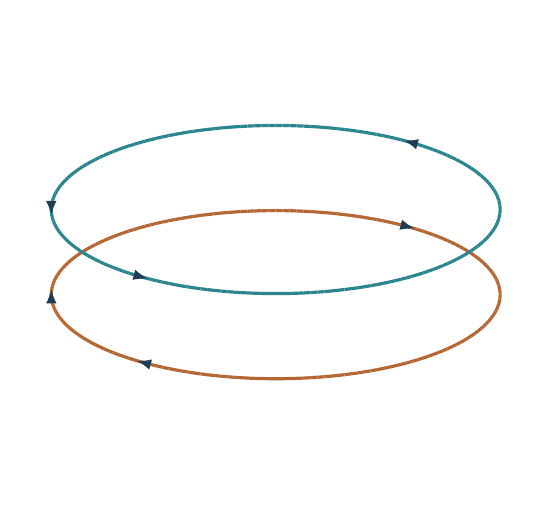
\begin{tikzpicture}[x=1cm,y=1cm,>=Latex,font=\small]
\path[use as bounding box] (-3.15,-2.85) rectangle (3.15,2.85);
\draw[copper,line width=1.15pt] (-0.00246,0.52718)--(0.08618,0.52669);
\draw[copper,line width=1.15pt] (-0.09111,0.52663)--(-0.00246,0.52718);
\draw[copper,line width=1.15pt] (0.08618,0.52669)--(0.17474,0.52517);
\draw[copper,line width=1.15pt] (-0.17966,0.52506)--(-0.09111,0.52663);
\draw[copper,line width=1.15pt] (0.17474,0.52517)--(0.26314,0.52262);
\draw[copper,line width=1.15pt] (-0.26804,0.52245)--(-0.17966,0.52506);
\draw[copper,line width=1.15pt] (0.26314,0.52262)--(0.35128,0.51904);
\draw[copper,line width=1.15pt] (-0.35616,0.51881)--(-0.26804,0.52245);
\draw[copper,line width=1.15pt] (0.35128,0.51904)--(0.43907,0.51443);
\draw[copper,line width=1.15pt] (-0.44394,0.51415)--(-0.35616,0.51881);
\draw[copper,line width=1.15pt] (0.43907,0.51443)--(0.52645,0.50881);
\draw[copper,line width=1.15pt] (-0.53129,0.50847)--(-0.44394,0.51415);
\draw[copper,line width=1.15pt] (0.52645,0.50881)--(0.61331,0.50217);
\draw[copper,line width=1.15pt] (-0.61812,0.50177)--(-0.53129,0.50847);
\draw[copper,line width=1.15pt] (0.61331,0.50217)--(0.69958,0.49452);
\draw[copper,line width=1.15pt] (-0.70436,0.49406)--(-0.61812,0.50177);
\draw[copper,line width=1.15pt] (0.69958,0.49452)--(0.78518,0.48587);
\draw[copper,line width=1.15pt] (-0.78991,0.48536)--(-0.70436,0.49406);
\draw[copper,line width=1.15pt] (0.78518,0.48587)--(0.87001,0.47622);
\draw[copper,line width=1.15pt] (-0.87470,0.47566)--(-0.78991,0.48536);
\draw[copper,line width=1.15pt] (0.87001,0.47622)--(0.95401,0.46560);
\draw[copper,line width=1.15pt] (-0.95865,0.46498)--(-0.87470,0.47566);
\draw[copper,line width=1.15pt] (0.95401,0.46560)--(1.03708,0.45400);
\draw[copper,line width=1.15pt] (-1.04166,0.45332)--(-0.95865,0.46498);
\draw[copper,line width=1.15pt] (1.03708,0.45400)--(1.11914,0.44143);
\draw[copper,line width=1.15pt] (-1.12367,0.44071)--(-1.04166,0.45332);
\draw[copper,line width=1.15pt] (1.11914,0.44143)--(1.20013,0.42792);
\draw[copper,line width=1.15pt] (-1.20459,0.42714)--(-1.12367,0.44071);
\draw[copper,line width=1.15pt] (1.20013,0.42792)--(1.27995,0.41347);
\draw[copper,line width=1.15pt] (-1.28435,0.41264)--(-1.20459,0.42714);
\draw[copper,line width=1.15pt] (1.27995,0.41347)--(1.35853,0.39810);
\draw[copper,line width=1.15pt] (-1.36286,0.39721)--(-1.28435,0.41264);
\draw[copper,line width=1.15pt] (1.35853,0.39810)--(1.43580,0.38181);
\draw[copper,line width=1.15pt] (-1.44006,0.38088)--(-1.36286,0.39721);
\draw[copper,line width=1.15pt] (1.43580,0.38181)--(1.51169,0.36464);
\draw[copper,line width=1.15pt] (-1.51586,0.36366)--(-1.44006,0.38088);
\draw[copper,line width=1.15pt] (1.51169,0.36464)--(1.58610,0.34659);
\draw[copper,line width=1.15pt] (-1.59019,0.34556)--(-1.51586,0.36366);
\draw[teal,line width=1.15pt] (-0.00246,1.60831)--(0.08618,1.60782);
\draw[teal,line width=1.15pt] (-0.09111,1.60776)--(-0.00246,1.60831);
\draw[teal,line width=1.15pt] (0.08618,1.60782)--(0.17474,1.60630);
\draw[teal,line width=1.15pt] (-0.17966,1.60619)--(-0.09111,1.60776);
\draw[teal,line width=1.15pt] (0.17474,1.60630)--(0.26314,1.60375);
\draw[teal,line width=1.15pt] (-0.26804,1.60358)--(-0.17966,1.60619);
\draw[teal,line width=1.15pt] (0.26314,1.60375)--(0.35128,1.60017);
\draw[teal,line width=1.15pt] (-0.35616,1.59994)--(-0.26804,1.60358);
\draw[teal,line width=1.15pt] (0.35128,1.60017)--(0.43907,1.59556);
\draw[teal,line width=1.15pt] (-0.44394,1.59528)--(-0.35616,1.59994);
\draw[copper,line width=1.15pt] (1.58610,0.34659)--(1.65899,0.32768);
\draw[copper,line width=1.15pt] (-1.66299,0.32661)--(-1.59019,0.34556);
\draw[teal,line width=1.15pt] (0.43907,1.59556)--(0.52645,1.58994);
\draw[teal,line width=1.15pt] (-0.53129,1.58960)--(-0.44394,1.59528);
\draw[teal,line width=1.15pt] (0.52645,1.58994)--(0.61331,1.58330);
\draw[teal,line width=1.15pt] (-0.61812,1.58290)--(-0.53129,1.58960);
\draw[teal,line width=1.15pt] (0.61331,1.58330)--(0.69958,1.57565);
\draw[teal,line width=1.15pt] (-0.70436,1.57519)--(-0.61812,1.58290);
\draw[copper,line width=1.15pt] (1.65899,0.32768)--(1.73027,0.30794);
\draw[copper,line width=1.15pt] (-1.73418,0.30681)--(-1.66299,0.32661);
\draw[teal,line width=1.15pt] (0.69958,1.57565)--(0.78518,1.56700);
\draw[teal,line width=1.15pt] (-0.78991,1.56649)--(-0.70436,1.57519);
\draw[teal,line width=1.15pt] (0.78518,1.56700)--(0.87001,1.55735);
\draw[teal,line width=1.15pt] (-0.87470,1.55679)--(-0.78991,1.56649);
\draw[copper,line width=1.15pt] (1.73027,0.30794)--(1.79987,0.28737);
\draw[copper,line width=1.15pt] (-1.80369,0.28620)--(-1.73418,0.30681);
\draw[teal,line width=1.15pt] (0.87001,1.55735)--(0.95401,1.54672);
\draw[teal,line width=1.15pt] (-0.95865,1.54611)--(-0.87470,1.55679);
\draw[teal,line width=1.15pt] (0.95401,1.54672)--(1.03708,1.53512);
\draw[teal,line width=1.15pt] (-1.04166,1.53445)--(-0.95865,1.54611);
\draw[copper,line width=1.15pt] (1.79987,0.28737)--(1.86774,0.26600);
\draw[copper,line width=1.15pt] (-1.87146,0.26479)--(-1.80369,0.28620);
\draw[teal,line width=1.15pt] (1.03708,1.53512)--(1.11914,1.52256);
\draw[teal,line width=1.15pt] (-1.12367,1.52183)--(-1.04166,1.53445);
\draw[teal,line width=1.15pt] (1.11914,1.52256)--(1.20013,1.50905);
\draw[teal,line width=1.15pt] (-1.20459,1.50827)--(-1.12367,1.52183);
\draw[copper,line width=1.15pt] (1.86774,0.26600)--(1.93380,0.24385);
\draw[copper,line width=1.15pt] (-1.93741,0.24260)--(-1.87146,0.26479);
\draw[teal,line width=1.15pt] (1.20013,1.50905)--(1.27995,1.49460);
\draw[teal,line width=1.15pt] (-1.28435,1.49377)--(-1.20459,1.50827);
\draw[copper,line width=1.15pt] (1.93380,0.24385)--(1.99798,0.22094);
\draw[copper,line width=1.15pt] (-2.00149,0.21965)--(-1.93741,0.24260);
\draw[teal,line width=1.15pt] (1.27995,1.49460)--(1.35853,1.47922);
\draw[teal,line width=1.15pt] (-1.36286,1.47834)--(-1.28435,1.49377);
\draw[teal,line width=1.15pt] (1.35853,1.47922)--(1.43580,1.46294);
\draw[teal,line width=1.15pt] (-1.44006,1.46201)--(-1.36286,1.47834);
\draw[copper,line width=1.15pt] (1.99798,0.22094)--(2.06024,0.19729);
\draw[copper,line width=1.15pt] (-2.06364,0.19596)--(-2.00149,0.21965);
\draw[teal,line width=1.15pt] (1.43580,1.46294)--(1.51169,1.44577);
\draw[teal,line width=1.15pt] (-1.51586,1.44479)--(-1.44006,1.46201);
\draw[copper,line width=1.15pt] (2.06024,0.19729)--(2.12050,0.17294);
\draw[copper,line width=1.15pt] (-2.12378,0.17156)--(-2.06364,0.19596);
\draw[teal,line width=1.15pt] (1.51169,1.44577)--(1.58610,1.42772);
\draw[teal,line width=1.15pt] (-1.59019,1.42669)--(-1.51586,1.44479);
\draw[teal,line width=1.15pt] (1.58610,1.42772)--(1.65899,1.40881);
\draw[copper,line width=1.15pt] (2.12050,0.17294)--(2.17871,0.14789);
\draw[teal,line width=1.15pt] (-1.66299,1.40774)--(-1.59019,1.42669);
\draw[copper,line width=1.15pt] (-2.18188,0.14647)--(-2.12378,0.17156);
\draw[teal,line width=1.15pt] (1.65899,1.40881)--(1.73027,1.38906);
\draw[teal,line width=1.15pt] (-1.73418,1.38794)--(-1.66299,1.40774);
\draw[copper,line width=1.15pt] (2.17871,0.14789)--(2.23481,0.12217);
\draw[copper,line width=1.15pt] (-2.23786,0.12072)--(-2.18188,0.14647);
\draw[teal,line width=1.15pt] (1.73027,1.38906)--(1.79987,1.36850);
\draw[teal,line width=1.15pt] (-1.80369,1.36733)--(-1.73418,1.38794);
\draw[copper,line width=1.15pt] (2.23481,0.12217)--(2.28875,0.09581);
\draw[copper,line width=1.15pt] (-2.29168,0.09433)--(-2.23786,0.12072);
\draw[teal,line width=1.15pt] (1.79987,1.36850)--(1.86774,1.34713);
\draw[teal,line width=1.15pt] (-1.87146,1.34592)--(-1.80369,1.36733);
\draw[copper,line width=1.15pt] (2.28875,0.09581)--(2.34047,0.06884);
\draw[copper,line width=1.15pt] (-2.34328,0.06733)--(-2.29168,0.09433);
\draw[teal,line width=1.15pt] (1.86774,1.34713)--(1.93380,1.32498);
\draw[teal,line width=1.15pt] (-1.93741,1.32372)--(-1.87146,1.34592);
\draw[teal,line width=1.15pt] (1.93380,1.32498)--(1.99798,1.30207);
\draw[copper,line width=1.15pt] (2.34047,0.06884)--(2.38993,0.04128);
\draw[teal,line width=1.15pt] (-2.00149,1.30077)--(-1.93741,1.32372);
\draw[copper,line width=1.15pt] (-2.39261,0.03973)--(-2.34328,0.06733);
\draw[teal,line width=1.15pt] (1.99798,1.30207)--(2.06024,1.27842);
\draw[teal,line width=1.15pt] (-2.06364,1.27709)--(-2.00149,1.30077);
\draw[copper,line width=1.15pt] (2.38993,0.04128)--(2.43708,0.01316);
\draw[copper,line width=1.15pt] (-2.43963,0.01158)--(-2.39261,0.03973);
\draw[teal,line width=1.15pt] (2.06024,1.27842)--(2.12050,1.25406);
\draw[teal,line width=1.15pt] (-2.12378,1.25269)--(-2.06364,1.27709);
\draw[copper,line width=1.15pt] (2.43708,0.01316)--(2.48187,-0.01550);
\draw[copper,line width=1.15pt] (-2.48429,-0.01711)--(-2.43963,0.01158);
\draw[teal,line width=1.15pt] (2.12050,1.25406)--(2.17871,1.22901);
\draw[teal,line width=1.15pt] (-2.18188,1.22760)--(-2.12378,1.25269);
\draw[copper,line width=1.15pt] (2.48187,-0.01550)--(2.52426,-0.04467);
\draw[copper,line width=1.15pt] (-2.52655,-0.04631)--(-2.48429,-0.01711);
\draw[teal,line width=1.15pt] (2.17871,1.22901)--(2.23481,1.20330);
\draw[teal,line width=1.15pt] (-2.23786,1.20185)--(-2.18188,1.22760);
\draw[copper,line width=1.15pt] (2.52426,-0.04467)--(2.56421,-0.07432);
\draw[copper,line width=1.15pt] (-2.56636,-0.07598)--(-2.52655,-0.04631);
\draw[teal,line width=1.15pt] (2.23481,1.20330)--(2.28875,1.17694);
\draw[teal,line width=1.15pt] (-2.29168,1.17546)--(-2.23786,1.20185);
\draw[copper,line width=1.15pt] (2.56421,-0.07432)--(2.60168,-0.10442);
\draw[copper,line width=1.15pt] (-2.60369,-0.10611)--(-2.56636,-0.07598);
\draw[teal,line width=1.15pt] (2.28875,1.17694)--(2.34047,1.14997);
\draw[teal,line width=1.15pt] (-2.34328,1.14845)--(-2.29168,1.17546);
\draw[copper,line width=1.15pt] (2.60168,-0.10442)--(2.63663,-0.13494);
\draw[copper,line width=1.15pt] (-2.63849,-0.13665)--(-2.60369,-0.10611);
\draw[teal,line width=1.15pt] (2.34047,1.14997)--(2.38993,1.12241);
\draw[teal,line width=1.15pt] (-2.39261,1.12086)--(-2.34328,1.14845);
\draw[teal,line width=1.15pt] (2.38993,1.12241)--(2.43708,1.09428);
\draw[copper,line width=1.15pt] (2.63663,-0.13494)--(2.66903,-0.16585);
\draw[teal,line width=1.15pt] (-2.43963,1.09271)--(-2.39261,1.12086);
\draw[copper,line width=1.15pt] (-2.67075,-0.16758)--(-2.63849,-0.13665);
\draw[teal,line width=1.15pt] (2.43708,1.09428)--(2.48187,1.06562);
\draw[teal,line width=1.15pt] (-2.48429,1.06402)--(-2.43963,1.09271);
\draw[copper,line width=1.15pt] (2.66903,-0.16585)--(2.69884,-0.19713);
\draw[copper,line width=1.15pt] (-2.70042,-0.19888)--(-2.67075,-0.16758);
\draw[teal,line width=1.15pt] (2.48187,1.06562)--(2.52426,1.03646);
\draw[teal,line width=1.15pt] (-2.52655,1.03482)--(-2.48429,1.06402);
\draw[copper,line width=1.15pt] (2.69884,-0.19713)--(2.72605,-0.22874);
\draw[copper,line width=1.15pt] (-2.72748,-0.23050)--(-2.70042,-0.19888);
\draw[teal,line width=1.15pt] (2.52426,1.03646)--(2.56421,1.00681);
\draw[teal,line width=1.15pt] (-2.56636,1.00515)--(-2.52655,1.03482);
\draw[copper,line width=1.15pt] (2.72605,-0.22874)--(2.75062,-0.26065);
\draw[copper,line width=1.15pt] (-2.75191,-0.26243)--(-2.72748,-0.23050);
\draw[teal,line width=1.15pt] (2.56421,1.00681)--(2.60168,0.97671);
\draw[teal,line width=1.15pt] (-2.60369,0.97502)--(-2.56636,1.00515);
\draw[copper,line width=1.15pt] (2.75062,-0.26065)--(2.77253,-0.29283);
\draw[copper,line width=1.15pt] (-2.77367,-0.29462)--(-2.75191,-0.26243);
\draw[teal,line width=1.15pt] (2.60168,0.97671)--(2.63663,0.94619);
\draw[teal,line width=1.15pt] (-2.63849,0.94448)--(-2.60369,0.97502);
\draw[copper,line width=1.15pt] (2.77253,-0.29283)--(2.79175,-0.32525);
\draw[copper,line width=1.15pt] (-2.79274,-0.32706)--(-2.77367,-0.29462);
\draw[teal,line width=1.15pt] (2.63663,0.94619)--(2.66903,0.91527);
\draw[teal,line width=1.15pt] (-2.67075,0.91355)--(-2.63849,0.94448);
\draw[copper,line width=1.15pt] (2.79175,-0.32525)--(2.80828,-0.35788);
\draw[copper,line width=1.15pt] (-2.80912,-0.35970)--(-2.79274,-0.32706);
\draw[teal,line width=1.15pt] (2.66903,0.91527)--(2.69884,0.88400);
\draw[teal,line width=1.15pt] (-2.70042,0.88225)--(-2.67075,0.91355);
\draw[copper,line width=1.15pt] (2.80828,-0.35788)--(2.82209,-0.39068);
\draw[copper,line width=1.15pt] (-2.82277,-0.39251)--(-2.80912,-0.35970);
\draw[teal,line width=1.15pt] (2.69884,0.88400)--(2.72605,0.85239);
\draw[teal,line width=1.15pt] (-2.72748,0.85062)--(-2.70042,0.88225);
\draw[copper,line width=1.15pt] (2.82209,-0.39068)--(2.83316,-0.42363);
\draw[copper,line width=1.15pt] (-2.83370,-0.42547)--(-2.82277,-0.39251);
\draw[teal,line width=1.15pt] (2.72605,0.85239)--(2.75062,0.82048);
\draw[teal,line width=1.15pt] (-2.75191,0.81870)--(-2.72748,0.85062);
\draw[copper,line width=1.15pt] (2.83316,-0.42363)--(2.84150,-0.45670);
\draw[copper,line width=1.15pt] (-2.84188,-0.45854)--(-2.83370,-0.42547);
\draw[teal,line width=1.15pt] (2.75062,0.82048)--(2.77253,0.78830);
\draw[teal,line width=1.15pt] (-2.77367,0.78650)--(-2.75191,0.81870);
\draw[copper,line width=1.15pt] (2.84150,-0.45670)--(2.84709,-0.48984);
\draw[copper,line width=1.15pt] (-2.84732,-0.49169)--(-2.84188,-0.45854);
\draw[teal,line width=1.15pt] (2.77253,0.78830)--(2.79175,0.75588);
\draw[teal,line width=1.15pt] (-2.79274,0.75407)--(-2.77367,0.78650);
\draw[copper,line width=1.15pt] (2.84709,-0.48984)--(2.84992,-0.52304);
\draw[copper,line width=1.15pt] (-2.85000,-0.52488)--(-2.84732,-0.49169);
\draw[teal,line width=1.15pt] (2.79175,0.75588)--(2.80828,0.72325);
\draw[teal,line width=1.15pt] (-2.80912,0.72143)--(-2.79274,0.75407);
\draw[copper,line width=1.15pt] (2.84992,-0.52304)--(2.85000,-0.55625);
\draw[copper,line width=1.15pt] (-2.84992,-0.55809)--(-2.85000,-0.52488);
\draw[teal,line width=1.15pt] (2.80828,0.72325)--(2.82209,0.69044);
\draw[teal,line width=1.15pt] (-2.82277,0.68862)--(-2.80912,0.72143);
\draw[copper,line width=1.15pt] (2.85000,-0.55625)--(2.84732,-0.58944);
\draw[copper,line width=1.15pt] (-2.84709,-0.59129)--(-2.84992,-0.55809);
\draw[teal,line width=1.15pt] (2.82209,0.69044)--(2.83316,0.65749);
\draw[teal,line width=1.15pt] (-2.83370,0.65566)--(-2.82277,0.68862);
\draw[copper,line width=1.15pt] (2.84732,-0.58944)--(2.84188,-0.62259);
\draw[copper,line width=1.15pt] (-2.84150,-0.62443)--(-2.84709,-0.59129);
\draw[teal,line width=1.15pt] (2.83316,0.65749)--(2.84150,0.62443);
\draw[teal,line width=1.15pt] (-2.84188,0.62259)--(-2.83370,0.65566);
\draw[copper,line width=1.15pt] (2.84188,-0.62259)--(2.83370,-0.65566);
\draw[copper,line width=1.15pt] (-2.83316,-0.65749)--(-2.84150,-0.62443);
\draw[teal,line width=1.15pt] (2.84150,0.62443)--(2.84709,0.59129);
\draw[teal,line width=1.15pt] (-2.84732,0.58944)--(-2.84188,0.62259);
\draw[copper,line width=1.15pt] (2.83370,-0.65566)--(2.82277,-0.68862);
\draw[copper,line width=1.15pt] (-2.82209,-0.69044)--(-2.83316,-0.65749);
\draw[teal,line width=1.15pt] (2.84709,0.59129)--(2.84992,0.55809);
\draw[teal,line width=1.15pt] (-2.85000,0.55625)--(-2.84732,0.58944);
\draw[copper,line width=1.15pt] (2.82277,-0.68862)--(2.80912,-0.72143);
\draw[copper,line width=1.15pt] (-2.80828,-0.72325)--(-2.82209,-0.69044);
\draw[teal,line width=1.15pt] (2.84992,0.55809)--(2.85000,0.52488);
\draw[teal,line width=1.15pt] (-2.84992,0.52304)--(-2.85000,0.55625);
\draw[copper,line width=1.15pt] (2.80912,-0.72143)--(2.79274,-0.75407);
\draw[copper,line width=1.15pt] (-2.79175,-0.75588)--(-2.80828,-0.72325);
\draw[teal,line width=1.15pt] (2.85000,0.52488)--(2.84732,0.49169);
\draw[teal,line width=1.15pt] (-2.84709,0.48984)--(-2.84992,0.52304);
\draw[copper,line width=1.15pt] (2.79274,-0.75407)--(2.77367,-0.78650);
\draw[copper,line width=1.15pt] (-2.77253,-0.78830)--(-2.79175,-0.75588);
\draw[teal,line width=1.15pt] (2.84732,0.49169)--(2.84188,0.45854);
\draw[teal,line width=1.15pt] (-2.84150,0.45670)--(-2.84709,0.48984);
\draw[copper,line width=1.15pt] (2.77367,-0.78650)--(2.75191,-0.81870);
\draw[copper,line width=1.15pt] (-2.75062,-0.82048)--(-2.77253,-0.78830);
\draw[teal,line width=1.15pt] (2.84188,0.45854)--(2.83370,0.42547);
\draw[teal,line width=1.15pt] (-2.83316,0.42363)--(-2.84150,0.45670);
\draw[copper,line width=1.15pt] (2.75191,-0.81870)--(2.72748,-0.85062);
\draw[copper,line width=1.15pt] (-2.72605,-0.85239)--(-2.75062,-0.82048);
\draw[teal,line width=1.15pt] (2.83370,0.42547)--(2.82277,0.39251);
\draw[teal,line width=1.15pt] (-2.82209,0.39068)--(-2.83316,0.42363);
\draw[copper,line width=1.15pt] (2.72748,-0.85062)--(2.70042,-0.88225);
\draw[copper,line width=1.15pt] (-2.69884,-0.88400)--(-2.72605,-0.85239);
\draw[teal,line width=1.15pt] (2.82277,0.39251)--(2.80912,0.35970);
\draw[teal,line width=1.15pt] (-2.80828,0.35788)--(-2.82209,0.39068);
\draw[copper,line width=1.15pt] (2.70042,-0.88225)--(2.67075,-0.91355);
\draw[copper,line width=1.15pt] (-2.66903,-0.91527)--(-2.69884,-0.88400);
\draw[teal,line width=1.15pt] (2.80912,0.35970)--(2.79274,0.32706);
\draw[teal,line width=1.15pt] (-2.79175,0.32525)--(-2.80828,0.35788);
\draw[copper,line width=1.15pt] (2.67075,-0.91355)--(2.63849,-0.94448);
\draw[copper,line width=1.15pt] (-2.63663,-0.94619)--(-2.66903,-0.91527);
\draw[teal,line width=1.15pt] (2.79274,0.32706)--(2.77367,0.29462);
\draw[teal,line width=1.15pt] (-2.77253,0.29283)--(-2.79175,0.32525);
\draw[copper,line width=1.15pt] (2.63849,-0.94448)--(2.60369,-0.97502);
\draw[copper,line width=1.15pt] (-2.60168,-0.97671)--(-2.63663,-0.94619);
\draw[teal,line width=1.15pt] (2.77367,0.29462)--(2.75191,0.26243);
\draw[teal,line width=1.15pt] (-2.75062,0.26065)--(-2.77253,0.29283);
\draw[copper,line width=1.15pt] (2.60369,-0.97502)--(2.56636,-1.00515);
\draw[copper,line width=1.15pt] (-2.56421,-1.00681)--(-2.60168,-0.97671);
\draw[teal,line width=1.15pt] (2.75191,0.26243)--(2.72748,0.23050);
\draw[teal,line width=1.15pt] (-2.72605,0.22874)--(-2.75062,0.26065);
\draw[copper,line width=1.15pt] (2.56636,-1.00515)--(2.52655,-1.03482);
\draw[copper,line width=1.15pt] (-2.52426,-1.03646)--(-2.56421,-1.00681);
\draw[teal,line width=1.15pt] (2.72748,0.23050)--(2.70042,0.19888);
\draw[teal,line width=1.15pt] (-2.69884,0.19713)--(-2.72605,0.22874);
\draw[copper,line width=1.15pt] (2.52655,-1.03482)--(2.48429,-1.06402);
\draw[copper,line width=1.15pt] (-2.48187,-1.06562)--(-2.52426,-1.03646);
\draw[teal,line width=1.15pt] (2.70042,0.19888)--(2.67075,0.16758);
\draw[teal,line width=1.15pt] (-2.66903,0.16585)--(-2.69884,0.19713);
\draw[copper,line width=1.15pt] (2.48429,-1.06402)--(2.43963,-1.09271);
\draw[copper,line width=1.15pt] (-2.43708,-1.09428)--(-2.48187,-1.06562);
\draw[teal,line width=1.15pt] (2.67075,0.16758)--(2.63849,0.13665);
\draw[copper,line width=1.15pt] (2.43963,-1.09271)--(2.39261,-1.12086);
\draw[teal,line width=1.15pt] (-2.63663,0.13494)--(-2.66903,0.16585);
\draw[copper,line width=1.15pt] (-2.38993,-1.12241)--(-2.43708,-1.09428);
\draw[copper,line width=1.15pt] (2.39261,-1.12086)--(2.34328,-1.14845);
\draw[copper,line width=1.15pt] (-2.34047,-1.14997)--(-2.38993,-1.12241);
\draw[teal,line width=1.15pt] (2.63849,0.13665)--(2.60369,0.10611);
\draw[teal,line width=1.15pt] (-2.60168,0.10442)--(-2.63663,0.13494);
\draw[copper,line width=1.15pt] (2.34328,-1.14845)--(2.29168,-1.17546);
\draw[copper,line width=1.15pt] (-2.28875,-1.17694)--(-2.34047,-1.14997);
\draw[teal,line width=1.15pt] (2.60369,0.10611)--(2.56636,0.07598);
\draw[teal,line width=1.15pt] (-2.56421,0.07432)--(-2.60168,0.10442);
\draw[copper,line width=1.15pt] (2.29168,-1.17546)--(2.23786,-1.20185);
\draw[copper,line width=1.15pt] (-2.23481,-1.20330)--(-2.28875,-1.17694);
\draw[teal,line width=1.15pt] (2.56636,0.07598)--(2.52655,0.04631);
\draw[teal,line width=1.15pt] (-2.52426,0.04467)--(-2.56421,0.07432);
\draw[copper,line width=1.15pt] (2.23786,-1.20185)--(2.18188,-1.22760);
\draw[copper,line width=1.15pt] (-2.17871,-1.22901)--(-2.23481,-1.20330);
\draw[teal,line width=1.15pt] (2.52655,0.04631)--(2.48429,0.01711);
\draw[teal,line width=1.15pt] (-2.48187,0.01550)--(-2.52426,0.04467);
\draw[copper,line width=1.15pt] (2.18188,-1.22760)--(2.12378,-1.25269);
\draw[copper,line width=1.15pt] (-2.12050,-1.25406)--(-2.17871,-1.22901);
\draw[teal,line width=1.15pt] (2.48429,0.01711)--(2.43963,-0.01158);
\draw[teal,line width=1.15pt] (-2.43708,-0.01316)--(-2.48187,0.01550);
\draw[copper,line width=1.15pt] (2.12378,-1.25269)--(2.06364,-1.27709);
\draw[copper,line width=1.15pt] (-2.06024,-1.27842)--(-2.12050,-1.25406);
\draw[teal,line width=1.15pt] (2.43963,-0.01158)--(2.39261,-0.03973);
\draw[teal,line width=1.15pt] (-2.38993,-0.04128)--(-2.43708,-0.01316);
\draw[copper,line width=1.15pt] (2.06364,-1.27709)--(2.00149,-1.30077);
\draw[copper,line width=1.15pt] (-1.99798,-1.30207)--(-2.06024,-1.27842);
\draw[teal,line width=1.15pt] (2.39261,-0.03973)--(2.34328,-0.06733);
\draw[copper,line width=1.15pt] (2.00149,-1.30077)--(1.93741,-1.32372);
\draw[teal,line width=1.15pt] (-2.34047,-0.06884)--(-2.38993,-0.04128);
\draw[copper,line width=1.15pt] (-1.93380,-1.32498)--(-1.99798,-1.30207);
\draw[copper,line width=1.15pt] (1.93741,-1.32372)--(1.87146,-1.34592);
\draw[copper,line width=1.15pt] (-1.86774,-1.34713)--(-1.93380,-1.32498);
\draw[teal,line width=1.15pt] (2.34328,-0.06733)--(2.29168,-0.09433);
\draw[teal,line width=1.15pt] (-2.28875,-0.09581)--(-2.34047,-0.06884);
\draw[copper,line width=1.15pt] (1.87146,-1.34592)--(1.80369,-1.36733);
\draw[copper,line width=1.15pt] (-1.79987,-1.36850)--(-1.86774,-1.34713);
\draw[teal,line width=1.15pt] (2.29168,-0.09433)--(2.23786,-0.12072);
\draw[teal,line width=1.15pt] (-2.23481,-0.12217)--(-2.28875,-0.09581);
\draw[copper,line width=1.15pt] (1.80369,-1.36733)--(1.73418,-1.38794);
\draw[copper,line width=1.15pt] (-1.73027,-1.38906)--(-1.79987,-1.36850);
\draw[teal,line width=1.15pt] (2.23786,-0.12072)--(2.18188,-0.14647);
\draw[teal,line width=1.15pt] (-2.17871,-0.14789)--(-2.23481,-0.12217);
\draw[copper,line width=1.15pt] (1.73418,-1.38794)--(1.66299,-1.40774);
\draw[copper,line width=1.15pt] (-1.65899,-1.40881)--(-1.73027,-1.38906);
\draw[teal,line width=1.15pt] (2.18188,-0.14647)--(2.12378,-0.17156);
\draw[copper,line width=1.15pt] (1.66299,-1.40774)--(1.59019,-1.42669);
\draw[teal,line width=1.15pt] (-2.12050,-0.17294)--(-2.17871,-0.14789);
\draw[copper,line width=1.15pt] (-1.58610,-1.42772)--(-1.65899,-1.40881);
\draw[copper,line width=1.15pt] (1.59019,-1.42669)--(1.51586,-1.44479);
\draw[copper,line width=1.15pt] (-1.51169,-1.44577)--(-1.58610,-1.42772);
\draw[teal,line width=1.15pt] (2.12378,-0.17156)--(2.06364,-0.19596);
\draw[teal,line width=1.15pt] (-2.06024,-0.19729)--(-2.12050,-0.17294);
\draw[copper,line width=1.15pt] (1.51586,-1.44479)--(1.44006,-1.46201);
\draw[copper,line width=1.15pt] (-1.43580,-1.46294)--(-1.51169,-1.44577);
\draw[teal,line width=1.15pt] (2.06364,-0.19596)--(2.00149,-0.21965);
\draw[teal,line width=1.15pt] (-1.99798,-0.22094)--(-2.06024,-0.19729);
\draw[copper,line width=1.15pt] (1.44006,-1.46201)--(1.36286,-1.47834);
\draw[copper,line width=1.15pt] (-1.35853,-1.47922)--(-1.43580,-1.46294);
\draw[copper,line width=1.15pt] (1.36286,-1.47834)--(1.28435,-1.49377);
\draw[copper,line width=1.15pt] (-1.27995,-1.49460)--(-1.35853,-1.47922);
\draw[teal,line width=1.15pt] (2.00149,-0.21965)--(1.93741,-0.24260);
\draw[teal,line width=1.15pt] (-1.93380,-0.24385)--(-1.99798,-0.22094);
\draw[copper,line width=1.15pt] (1.28435,-1.49377)--(1.20459,-1.50827);
\draw[copper,line width=1.15pt] (-1.20013,-1.50905)--(-1.27995,-1.49460);
\draw[teal,line width=1.15pt] (1.93741,-0.24260)--(1.87146,-0.26479);
\draw[teal,line width=1.15pt] (-1.86774,-0.26600)--(-1.93380,-0.24385);
\draw[copper,line width=1.15pt] (1.20459,-1.50827)--(1.12367,-1.52183);
\draw[copper,line width=1.15pt] (-1.11914,-1.52256)--(-1.20013,-1.50905);
\draw[copper,line width=1.15pt] (1.12367,-1.52183)--(1.04166,-1.53445);
\draw[copper,line width=1.15pt] (-1.03708,-1.53512)--(-1.11914,-1.52256);
\draw[teal,line width=1.15pt] (1.87146,-0.26479)--(1.80369,-0.28620);
\draw[teal,line width=1.15pt] (-1.79987,-0.28737)--(-1.86774,-0.26600);
\draw[copper,line width=1.15pt] (1.04166,-1.53445)--(0.95865,-1.54611);
\draw[copper,line width=1.15pt] (-0.95401,-1.54672)--(-1.03708,-1.53512);
\draw[copper,line width=1.15pt] (0.95865,-1.54611)--(0.87470,-1.55679);
\draw[copper,line width=1.15pt] (-0.87001,-1.55735)--(-0.95401,-1.54672);
\draw[teal,line width=1.15pt] (1.80369,-0.28620)--(1.73418,-0.30681);
\draw[teal,line width=1.15pt] (-1.73027,-0.30794)--(-1.79987,-0.28737);
\draw[copper,line width=1.15pt] (0.87470,-1.55679)--(0.78991,-1.56649);
\draw[copper,line width=1.15pt] (-0.78518,-1.56700)--(-0.87001,-1.55735);
\draw[copper,line width=1.15pt] (0.78991,-1.56649)--(0.70436,-1.57519);
\draw[copper,line width=1.15pt] (-0.69958,-1.57565)--(-0.78518,-1.56700);
\draw[teal,line width=1.15pt] (1.73418,-0.30681)--(1.66299,-0.32661);
\draw[teal,line width=1.15pt] (-1.65899,-0.32768)--(-1.73027,-0.30794);
\draw[copper,line width=1.15pt] (0.70436,-1.57519)--(0.61812,-1.58290);
\draw[copper,line width=1.15pt] (-0.61331,-1.58330)--(-0.69958,-1.57565);
\draw[copper,line width=1.15pt] (0.61812,-1.58290)--(0.53129,-1.58960);
\draw[copper,line width=1.15pt] (-0.52645,-1.58994)--(-0.61331,-1.58330);
\draw[copper,line width=1.15pt] (0.53129,-1.58960)--(0.44394,-1.59528);
\draw[copper,line width=1.15pt] (-0.43907,-1.59556)--(-0.52645,-1.58994);
\draw[teal,line width=1.15pt] (1.66299,-0.32661)--(1.59019,-0.34556);
\draw[teal,line width=1.15pt] (-1.58610,-0.34659)--(-1.65899,-0.32768);
\draw[copper,line width=1.15pt] (0.44394,-1.59528)--(0.35616,-1.59994);
\draw[copper,line width=1.15pt] (-0.35128,-1.60017)--(-0.43907,-1.59556);
\draw[copper,line width=1.15pt] (0.35616,-1.59994)--(0.26804,-1.60358);
\draw[copper,line width=1.15pt] (-0.26314,-1.60375)--(-0.35128,-1.60017);
\draw[copper,line width=1.15pt] (0.26804,-1.60358)--(0.17966,-1.60619);
\draw[copper,line width=1.15pt] (-0.17474,-1.60630)--(-0.26314,-1.60375);
\draw[copper,line width=1.15pt] (0.17966,-1.60619)--(0.09111,-1.60776);
\draw[copper,line width=1.15pt] (-0.08618,-1.60782)--(-0.17474,-1.60630);
\draw[copper,line width=1.15pt] (0.09111,-1.60776)--(0.00246,-1.60831);
\draw[copper,line width=1.15pt] (0.00246,-1.60831)--(-0.08618,-1.60782);
\draw[teal,line width=1.15pt] (1.59019,-0.34556)--(1.51586,-0.36366);
\draw[teal,line width=1.15pt] (-1.51169,-0.36464)--(-1.58610,-0.34659);
\draw[teal,line width=1.15pt] (1.51586,-0.36366)--(1.44006,-0.38088);
\draw[teal,line width=1.15pt] (-1.43580,-0.38181)--(-1.51169,-0.36464);
\draw[teal,line width=1.15pt] (1.44006,-0.38088)--(1.36286,-0.39721);
\draw[teal,line width=1.15pt] (-1.35853,-0.39810)--(-1.43580,-0.38181);
\draw[teal,line width=1.15pt] (1.36286,-0.39721)--(1.28435,-0.41264);
\draw[teal,line width=1.15pt] (-1.27995,-0.41347)--(-1.35853,-0.39810);
\draw[teal,line width=1.15pt] (1.28435,-0.41264)--(1.20459,-0.42714);
\draw[teal,line width=1.15pt] (-1.20013,-0.42792)--(-1.27995,-0.41347);
\draw[teal,line width=1.15pt] (1.20459,-0.42714)--(1.12367,-0.44071);
\draw[teal,line width=1.15pt] (-1.11914,-0.44143)--(-1.20013,-0.42792);
\draw[teal,line width=1.15pt] (1.12367,-0.44071)--(1.04166,-0.45332);
\draw[teal,line width=1.15pt] (-1.03708,-0.45400)--(-1.11914,-0.44143);
\draw[teal,line width=1.15pt] (1.04166,-0.45332)--(0.95865,-0.46498);
\draw[teal,line width=1.15pt] (-0.95401,-0.46560)--(-1.03708,-0.45400);
\draw[teal,line width=1.15pt] (0.95865,-0.46498)--(0.87470,-0.47566);
\draw[teal,line width=1.15pt] (-0.87001,-0.47622)--(-0.95401,-0.46560);
\draw[teal,line width=1.15pt] (0.87470,-0.47566)--(0.78991,-0.48536);
\draw[teal,line width=1.15pt] (-0.78518,-0.48587)--(-0.87001,-0.47622);
\draw[teal,line width=1.15pt] (0.78991,-0.48536)--(0.70436,-0.49406);
\draw[teal,line width=1.15pt] (-0.69958,-0.49452)--(-0.78518,-0.48587);
\draw[teal,line width=1.15pt] (0.70436,-0.49406)--(0.61812,-0.50177);
\draw[teal,line width=1.15pt] (-0.61331,-0.50217)--(-0.69958,-0.49452);
\draw[teal,line width=1.15pt] (0.61812,-0.50177)--(0.53129,-0.50847);
\draw[teal,line width=1.15pt] (-0.52645,-0.50881)--(-0.61331,-0.50217);
\draw[teal,line width=1.15pt] (0.53129,-0.50847)--(0.44394,-0.51415);
\draw[teal,line width=1.15pt] (-0.43907,-0.51443)--(-0.52645,-0.50881);
\draw[teal,line width=1.15pt] (0.44394,-0.51415)--(0.35616,-0.51881);
\draw[teal,line width=1.15pt] (-0.35128,-0.51904)--(-0.43907,-0.51443);
\draw[teal,line width=1.15pt] (0.35616,-0.51881)--(0.26804,-0.52245);
\draw[teal,line width=1.15pt] (-0.26314,-0.52262)--(-0.35128,-0.51904);
\draw[teal,line width=1.15pt] (0.26804,-0.52245)--(0.17966,-0.52506);
\draw[teal,line width=1.15pt] (-0.17474,-0.52517)--(-0.26314,-0.52262);
\draw[teal,line width=1.15pt] (0.17966,-0.52506)--(0.09111,-0.52663);
\draw[teal,line width=1.15pt] (-0.08618,-0.52669)--(-0.17474,-0.52517);
\draw[teal,line width=1.15pt] (0.09111,-0.52663)--(0.00246,-0.52718);
\draw[teal,line width=1.15pt] (0.00246,-0.52718)--(-0.08618,-0.52669);
\draw[navy,line width=.65pt,-{Latex[length=1.8mm]}] (1.62717,0.33650)--(1.76209,0.29912);
\draw[navy,line width=.65pt,-{Latex[length=1.8mm]}] (-2.84980,-0.61149)--(-2.85012,-0.47149);
\draw[navy,line width=.65pt,-{Latex[length=1.8mm]}] (-1.62717,-1.41763)--(-1.76209,-1.38025);
\draw[navy,line width=.65pt,-{Latex[length=1.8mm]}] (1.76209,1.38025)--(1.62717,1.41763);
\draw[navy,line width=.65pt,-{Latex[length=1.8mm]}] (-2.85012,0.60964)--(-2.84980,0.46964);
\draw[navy,line width=.65pt,-{Latex[length=1.8mm]}] (-1.76209,-0.29912)--(-1.62717,-0.33650);
\end{tikzpicture}
\par\small 轴向双环：两环参考电流反相
\end{minipage}\hfill
\begin{minipage}[t]{.50\linewidth}\centering\vspace{0pt}
\resizebox{\linewidth}{!}{%
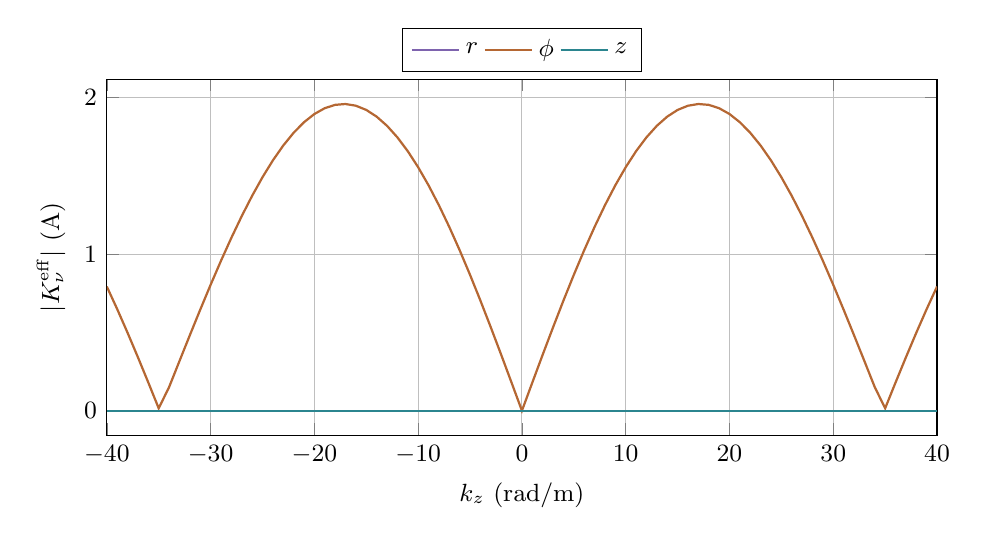
\begin{tikzpicture}
\begin{axis}[width=\linewidth,height=6.1cm,grid=major,
xlabel={$k_z$ (rad/m)},ylabel={$|K^{\rm eff}_\nu|$ (A)},
tick label style={font=\small},label style={font=\small},
legend style={font=\small,at={(.5,1.02)},anchor=south,legend columns=3},
xmin=-40,xmax=40,enlarge y limits=.08]
\addplot[violet,thick,no marks] coordinates {(-40,0) (-39,0) (-38,0) (-37,0) (-36,0) (-35,0) (-34,0) (-33,0) (-32,0) (-31,0) (-30,0) (-29,0) (-28,0) (-27,0) (-26,0) (-25,0) (-24,0) (-23,0) (-22,0) (-21,0) (-20,0) (-19,0) (-18,0) (-17,0) (-16,0) (-15,0) (-14,0) (-13,0) (-12,0) (-11,0) (-10,0) (-9,0) (-8,0) (-7,0) (-6,0) (-5,0) (-4,0) (-3,0) (-2,0) (-1,0) (0,0) (1,0) (2,0) (3,0) (4,0) (5,0) (6,0) (7,0) (8,0) (9,0) (10,0) (11,0) (12,0) (13,0) (14,0) (15,0) (16,0) (17,0) (18,0) (19,0) (20,0) (21,0) (22,0) (23,0) (24,0) (25,0) (26,0) (27,0) (28,0) (29,0) (30,0) (31,0) (32,0) (33,0) (34,0) (35,0) (36,0) (37,0) (38,0) (39,0) (40,0)};
\addlegendentry{$r$}
\addplot[copper,thick,no marks] coordinates {(-40,0.793611838363) (-39,0.649415608188) (-38,0.498243707976) (-37,0.341325750107) (-36,0.179954490995) (-35,0.0154745641569) (-34,0.150729366086) (-33,0.317244920713) (-32,0.48264467708) (-31,0.645499075924) (-30,0.804389442182) (-29,0.957920995709) (-28,1.10473572733) (-27,1.24352501629) (-26,1.37304186698) (-25,1.49211264597) (-24,1.59964820449) (-23,1.69465427718) (-22,1.77624105411) (-21,1.84363183091) (-20,1.89617065039) (-19,1.93332885826) (-18,1.95471050602) (-17,1.96005654488) (-16,1.94924776615) (-15,1.92230645566) (-14,1.87939674173) (-13,1.82082362939) (-12,1.74703072579) (-11,1.65859667451) (-10,1.55623032929) (-9,1.44076470961) (-8,1.31314979259) (-7,1.17444420714) (-6,1.02580590679) (-5,0.868481907879) (-4,0.703797188635) (-3,0.533142853263) (-2,0.357963672051) (-1,0.179745114829) (0,1.34021516144e-15) (1,0.179745114829) (2,0.357963672051) (3,0.533142853263) (4,0.703797188635) (5,0.868481907879) (6,1.02580590679) (7,1.17444420714) (8,1.31314979259) (9,1.44076470961) (10,1.55623032929) (11,1.65859667451) (12,1.74703072579) (13,1.82082362939) (14,1.87939674173) (15,1.92230645566) (16,1.94924776615) (17,1.96005654488) (18,1.95471050602) (19,1.93332885826) (20,1.89617065039) (21,1.84363183091) (22,1.77624105411) (23,1.69465427718) (24,1.59964820449) (25,1.49211264597) (26,1.37304186698) (27,1.24352501629) (28,1.10473572733) (29,0.957920995709) (30,0.804389442182) (31,0.645499075924) (32,0.48264467708) (33,0.317244920713) (34,0.150729366086) (35,0.0154745641569) (36,0.179954490995) (37,0.341325750107) (38,0.498243707976) (39,0.649415608188) (40,0.793611838363)};
\addlegendentry{$\phi$}
\addplot[teal,thick,no marks] coordinates {(-40,0) (-39,0) (-38,0) (-37,0) (-36,0) (-35,0) (-34,0) (-33,0) (-32,0) (-31,0) (-30,0) (-29,0) (-28,0) (-27,0) (-26,0) (-25,0) (-24,0) (-23,0) (-22,0) (-21,0) (-20,0) (-19,0) (-18,0) (-17,0) (-16,0) (-15,0) (-14,0) (-13,0) (-12,0) (-11,0) (-10,0) (-9,0) (-8,0) (-7,0) (-6,0) (-5,0) (-4,0) (-3,0) (-2,0) (-1,0) (0,0) (1,0) (2,0) (3,0) (4,0) (5,0) (6,0) (7,0) (8,0) (9,0) (10,0) (11,0) (12,0) (13,0) (14,0) (15,0) (16,0) (17,0) (18,0) (19,0) (20,0) (21,0) (22,0) (23,0) (24,0) (25,0) (26,0) (27,0) (28,0) (29,0) (30,0) (31,0) (32,0) (33,0) (34,0) (35,0) (36,0) (37,0) (38,0) (39,0) (40,0)};
\addlegendentry{$z$}
\end{axis}\end{tikzpicture}}
\par\small 展示汇总谱，$m=0$；场加载保留各源半径。
\end{minipage}
% END GENERATED: prescribed_current_13
\end{center}

\subsection{平面螺旋（编号 14）}
在 $z=z_0$ 的平面取 Archimedean 中心线。局部参数为
\begin{equation}
 r(t)=a_s+(b-a_s)t,\quad\phi(t)=\Omega t,\quad z(t)=0,
 \qquad 0\le t\le1,\quad \Omega=\chi2\pi n_s,
\end{equation}
其中 $0<a_s<b<R$，$n_s>0$ 为匝数，$\chi=\pm1$ 为几何绕向。
沿整条曲线指定同一复电流 $I$；内外端点保留为开端，电荷按式\eqref{eq:prescribedCharge}解释。
线元为 $(\dd r,r\dd\phi,0)$，故
\begin{equation}\label{eq:spiralIntegral}
 \begin{pmatrix}K_r^{\rm eff}\\K_\phi^{\rm eff}\\K_z^{\rm eff}\end{pmatrix}
 =\frac{CW_z}{2\pi b}\int_0^1
 \begin{pmatrix}b-a_s\\\Omega[a_s+(b-a_s)t]\\0\end{pmatrix}
 \ee^{-\ii m\Omega t}\dd t .
\end{equation}
定义 $F_0(x)=\ee^{-\ii x/2}\sinc(x/2)$、
$F_1(x)=\int_0^1t\ee^{-\ii xt}\dd t=\ii F_0'(x)$，
有连续极限 $F_0(0)=1,F_1(0)=1/2$。积分结果为
\begin{equation}
 \begin{aligned}
 K_r^{\rm eff}&=\frac{CW_z}{2\pi b}(b-a_s)F_0(m\Omega),\\
 K_\phi^{\rm eff}&=\frac{CW_z\Omega}{2\pi b}
 [a_sF_0(m\Omega)+(b-a_s)F_1(m\Omega)],\qquad K_z^{\rm eff}=0.
 \end{aligned}
\end{equation}
螺旋路径不是均匀完整圆环，不能直接强制它只有 $m=0$。
径向源在 $a_s\le r\le b$ 连续分布，场方程加载时逐位置保留。
本模板没有真实端面窗：当前介质仍只随 $r$ 变化，轴向仍无限。
\begin{center}% BEGIN GENERATED: prescribed_current_14
% Current geometry exported by C; arrows show instantaneous real current at t=0.
\begin{minipage}[t]{.48\linewidth}\centering\vspace{0pt}
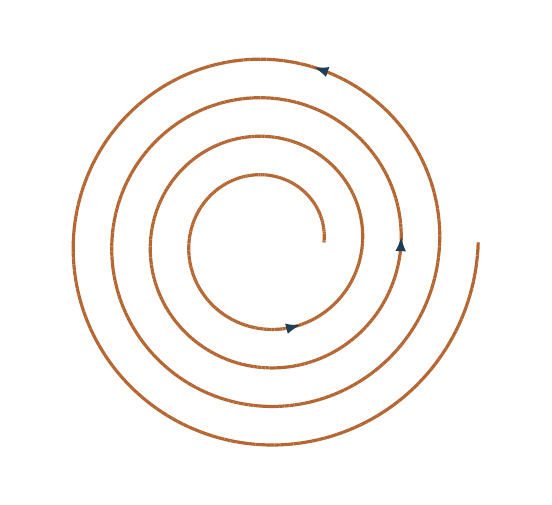
\begin{tikzpicture}[x=1cm,y=1cm,>=Latex,font=\small]
\path[use as bounding box] (-3.15,-2.85) rectangle (3.15,2.85);
\draw[copper,line width=1.15pt] (0.61274,0.12232)--(0.61481,0.14533);
\draw[copper,line width=1.15pt] (0.61481,0.14533)--(0.61616,0.16846);
\draw[copper,line width=1.15pt] (0.61616,0.16846)--(0.61679,0.19171);
\draw[copper,line width=1.15pt] (0.61679,0.19171)--(0.61668,0.21504);
\draw[copper,line width=1.15pt] (0.61668,0.21504)--(0.61582,0.23843);
\draw[copper,line width=1.15pt] (0.61582,0.23843)--(0.61423,0.26185);
\draw[copper,line width=1.15pt] (0.61423,0.26185)--(0.61189,0.28529);
\draw[copper,line width=1.15pt] (0.61189,0.28529)--(0.60881,0.30872);
\draw[copper,line width=1.15pt] (0.60881,0.30872)--(0.60497,0.33211);
\draw[copper,line width=1.15pt] (0.60497,0.33211)--(0.60038,0.35545);
\draw[copper,line width=1.15pt] (0.60038,0.35545)--(0.59504,0.37870);
\draw[copper,line width=1.15pt] (0.59504,0.37870)--(0.58896,0.40185);
\draw[copper,line width=1.15pt] (0.58896,0.40185)--(0.58212,0.42486);
\draw[copper,line width=1.15pt] (0.58212,0.42486)--(0.57454,0.44772);
\draw[copper,line width=1.15pt] (0.57454,0.44772)--(0.56621,0.47040);
\draw[copper,line width=1.15pt] (0.56621,0.47040)--(0.55715,0.49288);
\draw[copper,line width=1.15pt] (0.55715,0.49288)--(0.54735,0.51513);
\draw[copper,line width=1.15pt] (0.54735,0.51513)--(0.53682,0.53712);
\draw[copper,line width=1.15pt] (0.53682,0.53712)--(0.52557,0.55885);
\draw[copper,line width=1.15pt] (0.52557,0.55885)--(0.51360,0.58027);
\draw[copper,line width=1.15pt] (0.51360,0.58027)--(0.50092,0.60137);
\draw[copper,line width=1.15pt] (0.50092,0.60137)--(0.48755,0.62212);
\draw[copper,line width=1.15pt] (0.48755,0.62212)--(0.47348,0.64250);
\draw[copper,line width=1.15pt] (0.47348,0.64250)--(0.45874,0.66249);
\draw[copper,line width=1.15pt] (0.45874,0.66249)--(0.44332,0.68206);
\draw[copper,line width=1.15pt] (0.44332,0.68206)--(0.42725,0.70120);
\draw[copper,line width=1.15pt] (0.42725,0.70120)--(0.41053,0.71988);
\draw[copper,line width=1.15pt] (0.41053,0.71988)--(0.39318,0.73807);
\draw[copper,line width=1.15pt] (0.39318,0.73807)--(0.37521,0.75577);
\draw[copper,line width=1.15pt] (0.37521,0.75577)--(0.35663,0.77294);
\draw[copper,line width=1.15pt] (0.35663,0.77294)--(0.33747,0.78956);
\draw[copper,line width=1.15pt] (0.33747,0.78956)--(0.31774,0.80563);
\draw[copper,line width=1.15pt] (0.31774,0.80563)--(0.29744,0.82110);
\draw[copper,line width=1.15pt] (0.29744,0.82110)--(0.27661,0.83598);
\draw[copper,line width=1.15pt] (0.27661,0.83598)--(0.25526,0.85023);
\draw[copper,line width=1.15pt] (0.25526,0.85023)--(0.23341,0.86384);
\draw[copper,line width=1.15pt] (0.23341,0.86384)--(0.21107,0.87680);
\draw[copper,line width=1.15pt] (0.21107,0.87680)--(0.18827,0.88908);
\draw[copper,line width=1.15pt] (0.18827,0.88908)--(0.16502,0.90068);
\draw[copper,line width=1.15pt] (0.16502,0.90068)--(0.14135,0.91156);
\draw[copper,line width=1.15pt] (0.14135,0.91156)--(0.11729,0.92173);
\draw[copper,line width=1.15pt] (0.11729,0.92173)--(0.09284,0.93116);
\draw[copper,line width=1.15pt] (0.09284,0.93116)--(0.06804,0.93984);
\draw[copper,line width=1.15pt] (0.06804,0.93984)--(0.04290,0.94775);
\draw[copper,line width=1.15pt] (0.04290,0.94775)--(0.01746,0.95490);
\draw[copper,line width=1.15pt] (0.01746,0.95490)--(-0.00827,0.96125);
\draw[copper,line width=1.15pt] (-0.00827,0.96125)--(-0.03427,0.96681);
\draw[copper,line width=1.15pt] (-0.03427,0.96681)--(-0.06049,0.97157);
\draw[copper,line width=1.15pt] (-0.06049,0.97157)--(-0.08693,0.97550);
\draw[copper,line width=1.15pt] (-0.08693,0.97550)--(-0.11356,0.97861);
\draw[copper,line width=1.15pt] (-0.11356,0.97861)--(-0.14035,0.98089);
\draw[copper,line width=1.15pt] (-0.14035,0.98089)--(-0.16727,0.98232);
\draw[copper,line width=1.15pt] (-0.16727,0.98232)--(-0.19429,0.98291);
\draw[copper,line width=1.15pt] (-0.19429,0.98291)--(-0.22140,0.98265);
\draw[copper,line width=1.15pt] (-0.22140,0.98265)--(-0.24856,0.98153);
\draw[copper,line width=1.15pt] (-0.24856,0.98153)--(-0.27575,0.97956);
\draw[copper,line width=1.15pt] (-0.27575,0.97956)--(-0.30294,0.97672);
\draw[copper,line width=1.15pt] (-0.30294,0.97672)--(-0.33010,0.97302);
\draw[copper,line width=1.15pt] (-0.33010,0.97302)--(-0.35721,0.96845);
\draw[copper,line width=1.15pt] (-0.35721,0.96845)--(-0.38423,0.96301);
\draw[copper,line width=1.15pt] (-0.38423,0.96301)--(-0.41114,0.95671);
\draw[copper,line width=1.15pt] (-0.41114,0.95671)--(-0.43792,0.94955);
\draw[copper,line width=1.15pt] (-0.43792,0.94955)--(-0.46453,0.94153);
\draw[copper,line width=1.15pt] (-0.46453,0.94153)--(-0.49094,0.93265);
\draw[copper,line width=1.15pt] (-0.49094,0.93265)--(-0.51713,0.92292);
\draw[copper,line width=1.15pt] (-0.51713,0.92292)--(-0.54308,0.91234);
\draw[copper,line width=1.15pt] (-0.54308,0.91234)--(-0.56874,0.90092);
\draw[copper,line width=1.15pt] (-0.56874,0.90092)--(-0.59411,0.88866);
\draw[copper,line width=1.15pt] (-0.59411,0.88866)--(-0.61914,0.87558);
\draw[copper,line width=1.15pt] (-0.61914,0.87558)--(-0.64381,0.86168);
\draw[copper,line width=1.15pt] (-0.64381,0.86168)--(-0.66810,0.84697);
\draw[copper,line width=1.15pt] (-0.66810,0.84697)--(-0.69198,0.83147);
\draw[copper,line width=1.15pt] (-0.69198,0.83147)--(-0.71543,0.81517);
\draw[copper,line width=1.15pt] (-0.71543,0.81517)--(-0.73840,0.79811);
\draw[copper,line width=1.15pt] (-0.73840,0.79811)--(-0.76089,0.78028);
\draw[copper,line width=1.15pt] (-0.76089,0.78028)--(-0.78287,0.76170);
\draw[copper,line width=1.15pt] (-0.78287,0.76170)--(-0.80431,0.74240);
\draw[copper,line width=1.15pt] (-0.80431,0.74240)--(-0.82518,0.72237);
\draw[copper,line width=1.15pt] (-0.82518,0.72237)--(-0.84547,0.70165);
\draw[copper,line width=1.15pt] (-0.84547,0.70165)--(-0.86515,0.68024);
\draw[copper,line width=1.15pt] (-0.86515,0.68024)--(-0.88420,0.65817);
\draw[copper,line width=1.15pt] (-0.88420,0.65817)--(-0.90258,0.63545);
\draw[copper,line width=1.15pt] (-0.90258,0.63545)--(-0.92030,0.61210);
\draw[copper,line width=1.15pt] (-0.92030,0.61210)--(-0.93731,0.58815);
\draw[copper,line width=1.15pt] (-0.93731,0.58815)--(-0.95360,0.56361);
\draw[copper,line width=1.15pt] (-0.95360,0.56361)--(-0.96916,0.53850);
\draw[copper,line width=1.15pt] (-0.96916,0.53850)--(-0.98395,0.51286);
\draw[copper,line width=1.15pt] (-0.98395,0.51286)--(-0.99797,0.48669);
\draw[copper,line width=1.15pt] (-0.99797,0.48669)--(-1.01119,0.46003);
\draw[copper,line width=1.15pt] (-1.01119,0.46003)--(-1.02360,0.43290);
\draw[copper,line width=1.15pt] (-1.02360,0.43290)--(-1.03518,0.40532);
\draw[copper,line width=1.15pt] (-1.03518,0.40532)--(-1.04592,0.37733);
\draw[copper,line width=1.15pt] (-1.04592,0.37733)--(-1.05579,0.34893);
\draw[copper,line width=1.15pt] (-1.05579,0.34893)--(-1.06479,0.32017);
\draw[copper,line width=1.15pt] (-1.06479,0.32017)--(-1.07291,0.29107);
\draw[copper,line width=1.15pt] (-1.07291,0.29107)--(-1.08012,0.26165);
\draw[copper,line width=1.15pt] (-1.08012,0.26165)--(-1.08642,0.23194);
\draw[copper,line width=1.15pt] (-1.08642,0.23194)--(-1.09180,0.20198);
\draw[copper,line width=1.15pt] (-1.09180,0.20198)--(-1.09624,0.17179);
\draw[copper,line width=1.15pt] (-1.09624,0.17179)--(-1.09974,0.14140);
\draw[copper,line width=1.15pt] (-1.09974,0.14140)--(-1.10230,0.11084);
\draw[copper,line width=1.15pt] (-1.10230,0.11084)--(-1.10389,0.08014);
\draw[copper,line width=1.15pt] (-1.10389,0.08014)--(-1.10452,0.04932);
\draw[copper,line width=1.15pt] (-1.10452,0.04932)--(-1.10419,0.01843);
\draw[copper,line width=1.15pt] (-1.10419,0.01843)--(-1.10288,-0.01251);
\draw[copper,line width=1.15pt] (-1.10288,-0.01251)--(-1.10059,-0.04348);
\draw[copper,line width=1.15pt] (-1.10059,-0.04348)--(-1.09732,-0.07443);
\draw[copper,line width=1.15pt] (-1.09732,-0.07443)--(-1.09307,-0.10533);
\draw[copper,line width=1.15pt] (-1.09307,-0.10533)--(-1.08785,-0.13617);
\draw[copper,line width=1.15pt] (-1.08785,-0.13617)--(-1.08164,-0.16690);
\draw[copper,line width=1.15pt] (-1.08164,-0.16690)--(-1.07445,-0.19749);
\draw[copper,line width=1.15pt] (-1.07445,-0.19749)--(-1.06628,-0.22791);
\draw[copper,line width=1.15pt] (-1.06628,-0.22791)--(-1.05714,-0.25814);
\draw[copper,line width=1.15pt] (-1.05714,-0.25814)--(-1.04704,-0.28813);
\draw[copper,line width=1.15pt] (-1.04704,-0.28813)--(-1.03597,-0.31787);
\draw[copper,line width=1.15pt] (-1.03597,-0.31787)--(-1.02394,-0.34731);
\draw[copper,line width=1.15pt] (-1.02394,-0.34731)--(-1.01096,-0.37643);
\draw[copper,line width=1.15pt] (-1.01096,-0.37643)--(-0.99704,-0.40519);
\draw[copper,line width=1.15pt] (-0.99704,-0.40519)--(-0.98219,-0.43358);
\draw[copper,line width=1.15pt] (-0.98219,-0.43358)--(-0.96642,-0.46154);
\draw[copper,line width=1.15pt] (-0.96642,-0.46154)--(-0.94975,-0.48907);
\draw[copper,line width=1.15pt] (-0.94975,-0.48907)--(-0.93217,-0.51612);
\draw[copper,line width=1.15pt] (-0.93217,-0.51612)--(-0.91371,-0.54266);
\draw[copper,line width=1.15pt] (-0.91371,-0.54266)--(-0.89438,-0.56868);
\draw[copper,line width=1.15pt] (-0.89438,-0.56868)--(-0.87419,-0.59413);
\draw[copper,line width=1.15pt] (-0.87419,-0.59413)--(-0.85317,-0.61900);
\draw[copper,line width=1.15pt] (-0.85317,-0.61900)--(-0.83133,-0.64325);
\draw[copper,line width=1.15pt] (-0.83133,-0.64325)--(-0.80868,-0.66686);
\draw[copper,line width=1.15pt] (-0.80868,-0.66686)--(-0.78525,-0.68979);
\draw[copper,line width=1.15pt] (-0.78525,-0.68979)--(-0.76106,-0.71204);
\draw[copper,line width=1.15pt] (-0.76106,-0.71204)--(-0.73612,-0.73356);
\draw[copper,line width=1.15pt] (-0.73612,-0.73356)--(-0.71046,-0.75434);
\draw[copper,line width=1.15pt] (-0.71046,-0.75434)--(-0.68410,-0.77434);
\draw[copper,line width=1.15pt] (-0.68410,-0.77434)--(-0.65707,-0.79356);
\draw[copper,line width=1.15pt] (-0.65707,-0.79356)--(-0.62938,-0.81195);
\draw[copper,line width=1.15pt] (-0.62938,-0.81195)--(-0.60106,-0.82951);
\draw[copper,line width=1.15pt] (-0.60106,-0.82951)--(-0.57214,-0.84621);
\draw[copper,line width=1.15pt] (-0.57214,-0.84621)--(-0.54265,-0.86203);
\draw[copper,line width=1.15pt] (-0.54265,-0.86203)--(-0.51260,-0.87695);
\draw[copper,line width=1.15pt] (-0.51260,-0.87695)--(-0.48203,-0.89095);
\draw[copper,line width=1.15pt] (-0.48203,-0.89095)--(-0.45097,-0.90402);
\draw[copper,line width=1.15pt] (-0.45097,-0.90402)--(-0.41944,-0.91613);
\draw[copper,line width=1.15pt] (-0.41944,-0.91613)--(-0.38748,-0.92727);
\draw[copper,line width=1.15pt] (-0.38748,-0.92727)--(-0.35511,-0.93743);
\draw[copper,line width=1.15pt] (-0.35511,-0.93743)--(-0.32236,-0.94658);
\draw[copper,line width=1.15pt] (-0.32236,-0.94658)--(-0.28927,-0.95472);
\draw[copper,line width=1.15pt] (-0.28927,-0.95472)--(-0.25587,-0.96184);
\draw[copper,line width=1.15pt] (-0.25587,-0.96184)--(-0.22218,-0.96791);
\draw[copper,line width=1.15pt] (-0.22218,-0.96791)--(-0.18825,-0.97294);
\draw[copper,line width=1.15pt] (-0.18825,-0.97294)--(-0.15410,-0.97691);
\draw[copper,line width=1.15pt] (-0.15410,-0.97691)--(-0.11976,-0.97981);
\draw[copper,line width=1.15pt] (-0.11976,-0.97981)--(-0.08528,-0.98164);
\draw[copper,line width=1.15pt] (-0.08528,-0.98164)--(-0.05068,-0.98239);
\draw[copper,line width=1.15pt] (-0.05068,-0.98239)--(-0.01600,-0.98205);
\draw[copper,line width=1.15pt] (-0.01600,-0.98205)--(0.01873,-0.98062);
\draw[copper,line width=1.15pt] (0.01873,-0.98062)--(0.05347,-0.97809);
\draw[copper,line width=1.15pt] (0.05347,-0.97809)--(0.08820,-0.97447);
\draw[copper,line width=1.15pt] (0.08820,-0.97447)--(0.12286,-0.96975);
\draw[copper,line width=1.15pt] (0.12286,-0.96975)--(0.15744,-0.96394);
\draw[copper,line width=1.15pt] (0.15744,-0.96394)--(0.19189,-0.95702);
\draw[copper,line width=1.15pt] (0.19189,-0.95702)--(0.22618,-0.94902);
\draw[copper,line width=1.15pt] (0.22618,-0.94902)--(0.26028,-0.93992);
\draw[copper,line width=1.15pt] (0.26028,-0.93992)--(0.29415,-0.92973);
\draw[copper,line width=1.15pt] (0.29415,-0.92973)--(0.32775,-0.91847);
\draw[copper,line width=1.15pt] (0.32775,-0.91847)--(0.36105,-0.90613);
\draw[copper,line width=1.15pt] (0.36105,-0.90613)--(0.39402,-0.89272);
\draw[copper,line width=1.15pt] (0.39402,-0.89272)--(0.42663,-0.87825);
\draw[copper,line width=1.15pt] (0.42663,-0.87825)--(0.45883,-0.86274);
\draw[copper,line width=1.15pt] (0.45883,-0.86274)--(0.49060,-0.84619);
\draw[copper,line width=1.15pt] (0.49060,-0.84619)--(0.52190,-0.82861);
\draw[copper,line width=1.15pt] (0.52190,-0.82861)--(0.55269,-0.81002);
\draw[copper,line width=1.15pt] (0.55269,-0.81002)--(0.58295,-0.79043);
\draw[copper,line width=1.15pt] (0.58295,-0.79043)--(0.61265,-0.76987);
\draw[copper,line width=1.15pt] (0.61265,-0.76987)--(0.64175,-0.74833);
\draw[copper,line width=1.15pt] (0.64175,-0.74833)--(0.67021,-0.72585);
\draw[copper,line width=1.15pt] (0.67021,-0.72585)--(0.69802,-0.70243);
\draw[copper,line width=1.15pt] (0.69802,-0.70243)--(0.72513,-0.67811);
\draw[copper,line width=1.15pt] (0.72513,-0.67811)--(0.75153,-0.65289);
\draw[copper,line width=1.15pt] (0.75153,-0.65289)--(0.77717,-0.62681);
\draw[copper,line width=1.15pt] (0.77717,-0.62681)--(0.80203,-0.59987);
\draw[copper,line width=1.15pt] (0.80203,-0.59987)--(0.82609,-0.57212);
\draw[copper,line width=1.15pt] (0.82609,-0.57212)--(0.84931,-0.54356);
\draw[copper,line width=1.15pt] (0.84931,-0.54356)--(0.87167,-0.51423);
\draw[copper,line width=1.15pt] (0.87167,-0.51423)--(0.89315,-0.48416);
\draw[copper,line width=1.15pt] (0.89315,-0.48416)--(0.91371,-0.45336);
\draw[copper,line width=1.15pt] (0.91371,-0.45336)--(0.93334,-0.42186);
\draw[copper,line width=1.15pt] (0.93334,-0.42186)--(0.95201,-0.38971);
\draw[copper,line width=1.15pt] (0.95201,-0.38971)--(0.96970,-0.35691);
\draw[copper,line width=1.15pt] (0.96970,-0.35691)--(0.98639,-0.32351);
\draw[copper,line width=1.15pt] (0.98639,-0.32351)--(1.00205,-0.28953);
\draw[copper,line width=1.15pt] (1.00205,-0.28953)--(1.01667,-0.25501);
\draw[copper,line width=1.15pt] (1.01667,-0.25501)--(1.03022,-0.21998);
\draw[copper,line width=1.15pt] (1.03022,-0.21998)--(1.04270,-0.18447);
\draw[copper,line width=1.15pt] (1.04270,-0.18447)--(1.05408,-0.14851);
\draw[copper,line width=1.15pt] (1.05408,-0.14851)--(1.06435,-0.11214);
\draw[copper,line width=1.15pt] (1.06435,-0.11214)--(1.07349,-0.07540);
\draw[copper,line width=1.15pt] (1.07349,-0.07540)--(1.08149,-0.03831);
\draw[copper,line width=1.15pt] (1.08149,-0.03831)--(1.08834,-0.00091);
\draw[copper,line width=1.15pt] (1.08834,-0.00091)--(1.09402,0.03676);
\draw[copper,line width=1.15pt] (1.09402,0.03676)--(1.09853,0.07466);
\draw[copper,line width=1.15pt] (1.09853,0.07466)--(1.10186,0.11276);
\draw[copper,line width=1.15pt] (1.10186,0.11276)--(1.10399,0.15103);
\draw[copper,line width=1.15pt] (1.10399,0.15103)--(1.10493,0.18941);
\draw[copper,line width=1.15pt] (1.10493,0.18941)--(1.10466,0.22789);
\draw[copper,line width=1.15pt] (1.10466,0.22789)--(1.10319,0.26641);
\draw[copper,line width=1.15pt] (1.10319,0.26641)--(1.10050,0.30494);
\draw[copper,line width=1.15pt] (1.10050,0.30494)--(1.09660,0.34344);
\draw[copper,line width=1.15pt] (1.09660,0.34344)--(1.09148,0.38188);
\draw[copper,line width=1.15pt] (1.09148,0.38188)--(1.08515,0.42022);
\draw[copper,line width=1.15pt] (1.08515,0.42022)--(1.07761,0.45841);
\draw[copper,line width=1.15pt] (1.07761,0.45841)--(1.06885,0.49642);
\draw[copper,line width=1.15pt] (1.06885,0.49642)--(1.05889,0.53421);
\draw[copper,line width=1.15pt] (1.05889,0.53421)--(1.04773,0.57174);
\draw[copper,line width=1.15pt] (1.04773,0.57174)--(1.03537,0.60897);
\draw[copper,line width=1.15pt] (1.03537,0.60897)--(1.02183,0.64587);
\draw[copper,line width=1.15pt] (1.02183,0.64587)--(1.00711,0.68240);
\draw[copper,line width=1.15pt] (1.00711,0.68240)--(0.99122,0.71852);
\draw[copper,line width=1.15pt] (0.99122,0.71852)--(0.97418,0.75420);
\draw[copper,line width=1.15pt] (0.97418,0.75420)--(0.95599,0.78938);
\draw[copper,line width=1.15pt] (0.95599,0.78938)--(0.93667,0.82405);
\draw[copper,line width=1.15pt] (0.93667,0.82405)--(0.91623,0.85816);
\draw[copper,line width=1.15pt] (0.91623,0.85816)--(0.89470,0.89168);
\draw[copper,line width=1.15pt] (0.89470,0.89168)--(0.87208,0.92457);
\draw[copper,line width=1.15pt] (0.87208,0.92457)--(0.84840,0.95679);
\draw[copper,line width=1.15pt] (0.84840,0.95679)--(0.82367,0.98832);
\draw[copper,line width=1.15pt] (0.82367,0.98832)--(0.79792,1.01911);
\draw[copper,line width=1.15pt] (0.79792,1.01911)--(0.77117,1.04914);
\draw[copper,line width=1.15pt] (0.77117,1.04914)--(0.74343,1.07837);
\draw[copper,line width=1.15pt] (0.74343,1.07837)--(0.71474,1.10677);
\draw[copper,line width=1.15pt] (0.71474,1.10677)--(0.68512,1.13431);
\draw[copper,line width=1.15pt] (0.68512,1.13431)--(0.65460,1.16096);
\draw[copper,line width=1.15pt] (0.65460,1.16096)--(0.62319,1.18668);
\draw[copper,line width=1.15pt] (0.62319,1.18668)--(0.59094,1.21146);
\draw[copper,line width=1.15pt] (0.59094,1.21146)--(0.55786,1.23526);
\draw[copper,line width=1.15pt] (0.55786,1.23526)--(0.52399,1.25805);
\draw[copper,line width=1.15pt] (0.52399,1.25805)--(0.48936,1.27981);
\draw[copper,line width=1.15pt] (0.48936,1.27981)--(0.45400,1.30052);
\draw[copper,line width=1.15pt] (0.45400,1.30052)--(0.41794,1.32014);
\draw[copper,line width=1.15pt] (0.41794,1.32014)--(0.38121,1.33866);
\draw[copper,line width=1.15pt] (0.38121,1.33866)--(0.34386,1.35605);
\draw[copper,line width=1.15pt] (0.34386,1.35605)--(0.30591,1.37229);
\draw[copper,line width=1.15pt] (0.30591,1.37229)--(0.26740,1.38736);
\draw[copper,line width=1.15pt] (0.26740,1.38736)--(0.22836,1.40124);
\draw[copper,line width=1.15pt] (0.22836,1.40124)--(0.18884,1.41392);
\draw[copper,line width=1.15pt] (0.18884,1.41392)--(0.14886,1.42537);
\draw[copper,line width=1.15pt] (0.14886,1.42537)--(0.10848,1.43559);
\draw[copper,line width=1.15pt] (0.10848,1.43559)--(0.06771,1.44455);
\draw[copper,line width=1.15pt] (0.06771,1.44455)--(0.02662,1.45224);
\draw[copper,line width=1.15pt] (0.02662,1.45224)--(-0.01477,1.45866);
\draw[copper,line width=1.15pt] (-0.01477,1.45866)--(-0.05642,1.46378);
\draw[copper,line width=1.15pt] (-0.05642,1.46378)--(-0.09829,1.46760);
\draw[copper,line width=1.15pt] (-0.09829,1.46760)--(-0.14033,1.47012);
\draw[copper,line width=1.15pt] (-0.14033,1.47012)--(-0.18250,1.47132);
\draw[copper,line width=1.15pt] (-0.18250,1.47132)--(-0.22476,1.47120);
\draw[copper,line width=1.15pt] (-0.22476,1.47120)--(-0.26708,1.46975);
\draw[copper,line width=1.15pt] (-0.26708,1.46975)--(-0.30941,1.46697);
\draw[copper,line width=1.15pt] (-0.30941,1.46697)--(-0.35170,1.46286);
\draw[copper,line width=1.15pt] (-0.35170,1.46286)--(-0.39392,1.45742);
\draw[copper,line width=1.15pt] (-0.39392,1.45742)--(-0.43602,1.45065);
\draw[copper,line width=1.15pt] (-0.43602,1.45065)--(-0.47797,1.44254);
\draw[copper,line width=1.15pt] (-0.47797,1.44254)--(-0.51972,1.43311);
\draw[copper,line width=1.15pt] (-0.51972,1.43311)--(-0.56122,1.42236);
\draw[copper,line width=1.15pt] (-0.56122,1.42236)--(-0.60244,1.41030);
\draw[copper,line width=1.15pt] (-0.60244,1.41030)--(-0.64333,1.39692);
\draw[copper,line width=1.15pt] (-0.64333,1.39692)--(-0.68385,1.38225);
\draw[copper,line width=1.15pt] (-0.68385,1.38225)--(-0.72397,1.36628);
\draw[copper,line width=1.15pt] (-0.72397,1.36628)--(-0.76364,1.34904);
\draw[copper,line width=1.15pt] (-0.76364,1.34904)--(-0.80281,1.33053);
\draw[copper,line width=1.15pt] (-0.80281,1.33053)--(-0.84145,1.31077);
\draw[copper,line width=1.15pt] (-0.84145,1.31077)--(-0.87953,1.28977);
\draw[copper,line width=1.15pt] (-0.87953,1.28977)--(-0.91699,1.26755);
\draw[copper,line width=1.15pt] (-0.91699,1.26755)--(-0.95380,1.24413);
\draw[copper,line width=1.15pt] (-0.95380,1.24413)--(-0.98992,1.21952);
\draw[copper,line width=1.15pt] (-0.98992,1.21952)--(-1.02532,1.19375);
\draw[copper,line width=1.15pt] (-1.02532,1.19375)--(-1.05995,1.16684);
\draw[copper,line width=1.15pt] (-1.05995,1.16684)--(-1.09378,1.13881);
\draw[copper,line width=1.15pt] (-1.09378,1.13881)--(-1.12677,1.10968);
\draw[copper,line width=1.15pt] (-1.12677,1.10968)--(-1.15889,1.07948);
\draw[copper,line width=1.15pt] (-1.15889,1.07948)--(-1.19011,1.04824);
\draw[copper,line width=1.15pt] (-1.19011,1.04824)--(-1.22038,1.01598);
\draw[copper,line width=1.15pt] (-1.22038,1.01598)--(-1.24967,0.98273);
\draw[copper,line width=1.15pt] (-1.24967,0.98273)--(-1.27796,0.94852);
\draw[copper,line width=1.15pt] (-1.27796,0.94852)--(-1.30521,0.91339);
\draw[copper,line width=1.15pt] (-1.30521,0.91339)--(-1.33139,0.87735);
\draw[copper,line width=1.15pt] (-1.33139,0.87735)--(-1.35648,0.84045);
\draw[copper,line width=1.15pt] (-1.35648,0.84045)--(-1.38043,0.80272);
\draw[copper,line width=1.15pt] (-1.38043,0.80272)--(-1.40323,0.76420);
\draw[copper,line width=1.15pt] (-1.40323,0.76420)--(-1.42486,0.72491);
\draw[copper,line width=1.15pt] (-1.42486,0.72491)--(-1.44527,0.68489);
\draw[copper,line width=1.15pt] (-1.44527,0.68489)--(-1.46445,0.64419);
\draw[copper,line width=1.15pt] (-1.46445,0.64419)--(-1.48239,0.60284);
\draw[copper,line width=1.15pt] (-1.48239,0.60284)--(-1.49904,0.56088);
\draw[copper,line width=1.15pt] (-1.49904,0.56088)--(-1.51440,0.51834);
\draw[copper,line width=1.15pt] (-1.51440,0.51834)--(-1.52845,0.47527);
\draw[copper,line width=1.15pt] (-1.52845,0.47527)--(-1.54116,0.43171);
\draw[copper,line width=1.15pt] (-1.54116,0.43171)--(-1.55251,0.38770);
\draw[copper,line width=1.15pt] (-1.55251,0.38770)--(-1.56251,0.34329);
\draw[copper,line width=1.15pt] (-1.56251,0.34329)--(-1.57112,0.29850);
\draw[copper,line width=1.15pt] (-1.57112,0.29850)--(-1.57834,0.25340);
\draw[copper,line width=1.15pt] (-1.57834,0.25340)--(-1.58415,0.20801);
\draw[copper,line width=1.15pt] (-1.58415,0.20801)--(-1.58854,0.16239);
\draw[copper,line width=1.15pt] (-1.58854,0.16239)--(-1.59151,0.11658);
\draw[copper,line width=1.15pt] (-1.59151,0.11658)--(-1.59305,0.07062);
\draw[copper,line width=1.15pt] (-1.59305,0.07062)--(-1.59315,0.02457);
\draw[copper,line width=1.15pt] (-1.59315,0.02457)--(-1.59180,-0.02155);
\draw[copper,line width=1.15pt] (-1.59180,-0.02155)--(-1.58901,-0.06768);
\draw[copper,line width=1.15pt] (-1.58901,-0.06768)--(-1.58476,-0.11377);
\draw[copper,line width=1.15pt] (-1.58476,-0.11377)--(-1.57907,-0.15978);
\draw[copper,line width=1.15pt] (-1.57907,-0.15978)--(-1.57193,-0.20566);
\draw[copper,line width=1.15pt] (-1.57193,-0.20566)--(-1.56334,-0.25138);
\draw[copper,line width=1.15pt] (-1.56334,-0.25138)--(-1.55331,-0.29688);
\draw[copper,line width=1.15pt] (-1.55331,-0.29688)--(-1.54184,-0.34211);
\draw[copper,line width=1.15pt] (-1.54184,-0.34211)--(-1.52894,-0.38704);
\draw[copper,line width=1.15pt] (-1.52894,-0.38704)--(-1.51461,-0.43161);
\draw[copper,line width=1.15pt] (-1.51461,-0.43161)--(-1.49887,-0.47578);
\draw[copper,line width=1.15pt] (-1.49887,-0.47578)--(-1.48173,-0.51951);
\draw[copper,line width=1.15pt] (-1.48173,-0.51951)--(-1.46320,-0.56275);
\draw[copper,line width=1.15pt] (-1.46320,-0.56275)--(-1.44330,-0.60546);
\draw[copper,line width=1.15pt] (-1.44330,-0.60546)--(-1.42203,-0.64760);
\draw[copper,line width=1.15pt] (-1.42203,-0.64760)--(-1.39942,-0.68911);
\draw[copper,line width=1.15pt] (-1.39942,-0.68911)--(-1.37548,-0.72996);
\draw[copper,line width=1.15pt] (-1.37548,-0.72996)--(-1.35023,-0.77011);
\draw[copper,line width=1.15pt] (-1.35023,-0.77011)--(-1.32370,-0.80951);
\draw[copper,line width=1.15pt] (-1.32370,-0.80951)--(-1.29590,-0.84812);
\draw[copper,line width=1.15pt] (-1.29590,-0.84812)--(-1.26686,-0.88590);
\draw[copper,line width=1.15pt] (-1.26686,-0.88590)--(-1.23661,-0.92281);
\draw[copper,line width=1.15pt] (-1.23661,-0.92281)--(-1.20516,-0.95882);
\draw[copper,line width=1.15pt] (-1.20516,-0.95882)--(-1.17255,-0.99388);
\draw[copper,line width=1.15pt] (-1.17255,-0.99388)--(-1.13881,-1.02795);
\draw[copper,line width=1.15pt] (-1.13881,-1.02795)--(-1.10396,-1.06101);
\draw[copper,line width=1.15pt] (-1.10396,-1.06101)--(-1.06804,-1.09301);
\draw[copper,line width=1.15pt] (-1.06804,-1.09301)--(-1.03108,-1.12392);
\draw[copper,line width=1.15pt] (-1.03108,-1.12392)--(-0.99310,-1.15370);
\draw[copper,line width=1.15pt] (-0.99310,-1.15370)--(-0.95416,-1.18232);
\draw[copper,line width=1.15pt] (-0.95416,-1.18232)--(-0.91427,-1.20976);
\draw[copper,line width=1.15pt] (-0.91427,-1.20976)--(-0.87348,-1.23597);
\draw[copper,line width=1.15pt] (-0.87348,-1.23597)--(-0.83182,-1.26094);
\draw[copper,line width=1.15pt] (-0.83182,-1.26094)--(-0.78934,-1.28462);
\draw[copper,line width=1.15pt] (-0.78934,-1.28462)--(-0.74607,-1.30700);
\draw[copper,line width=1.15pt] (-0.74607,-1.30700)--(-0.70206,-1.32805);
\draw[copper,line width=1.15pt] (-0.70206,-1.32805)--(-0.65733,-1.34774);
\draw[copper,line width=1.15pt] (-0.65733,-1.34774)--(-0.61194,-1.36604);
\draw[copper,line width=1.15pt] (-0.61194,-1.36604)--(-0.56593,-1.38295);
\draw[copper,line width=1.15pt] (-0.56593,-1.38295)--(-0.51934,-1.39843);
\draw[copper,line width=1.15pt] (-0.51934,-1.39843)--(-0.47222,-1.41247);
\draw[copper,line width=1.15pt] (-0.47222,-1.41247)--(-0.42461,-1.42504);
\draw[copper,line width=1.15pt] (-0.42461,-1.42504)--(-0.37655,-1.43614);
\draw[copper,line width=1.15pt] (-0.37655,-1.43614)--(-0.32809,-1.44574);
\draw[copper,line width=1.15pt] (-0.32809,-1.44574)--(-0.27929,-1.45384);
\draw[copper,line width=1.15pt] (-0.27929,-1.45384)--(-0.23018,-1.46041);
\draw[copper,line width=1.15pt] (-0.23018,-1.46041)--(-0.18081,-1.46545);
\draw[copper,line width=1.15pt] (-0.18081,-1.46545)--(-0.13123,-1.46895);
\draw[copper,line width=1.15pt] (-0.13123,-1.46895)--(-0.08149,-1.47090);
\draw[copper,line width=1.15pt] (-0.08149,-1.47090)--(-0.03164,-1.47129);
\draw[copper,line width=1.15pt] (-0.03164,-1.47129)--(0.01827,-1.47012);
\draw[copper,line width=1.15pt] (0.01827,-1.47012)--(0.06820,-1.46738);
\draw[copper,line width=1.15pt] (0.06820,-1.46738)--(0.11810,-1.46308);
\draw[copper,line width=1.15pt] (0.11810,-1.46308)--(0.16791,-1.45721);
\draw[copper,line width=1.15pt] (0.16791,-1.45721)--(0.21759,-1.44977);
\draw[copper,line width=1.15pt] (0.21759,-1.44977)--(0.26709,-1.44077);
\draw[copper,line width=1.15pt] (0.26709,-1.44077)--(0.31635,-1.43020);
\draw[copper,line width=1.15pt] (0.31635,-1.43020)--(0.36533,-1.41809);
\draw[copper,line width=1.15pt] (0.36533,-1.41809)--(0.41399,-1.40442);
\draw[copper,line width=1.15pt] (0.41399,-1.40442)--(0.46226,-1.38922);
\draw[copper,line width=1.15pt] (0.46226,-1.38922)--(0.51011,-1.37249);
\draw[copper,line width=1.15pt] (0.51011,-1.37249)--(0.55748,-1.35424);
\draw[copper,line width=1.15pt] (0.55748,-1.35424)--(0.60432,-1.33449);
\draw[copper,line width=1.15pt] (0.60432,-1.33449)--(0.65060,-1.31326);
\draw[copper,line width=1.15pt] (0.65060,-1.31326)--(0.69626,-1.29055);
\draw[copper,line width=1.15pt] (0.69626,-1.29055)--(0.74124,-1.26639);
\draw[copper,line width=1.15pt] (0.74124,-1.26639)--(0.78552,-1.24079);
\draw[copper,line width=1.15pt] (0.78552,-1.24079)--(0.82904,-1.21378);
\draw[copper,line width=1.15pt] (0.82904,-1.21378)--(0.87176,-1.18538);
\draw[copper,line width=1.15pt] (0.87176,-1.18538)--(0.91363,-1.15562);
\draw[copper,line width=1.15pt] (0.91363,-1.15562)--(0.95460,-1.12451);
\draw[copper,line width=1.15pt] (0.95460,-1.12451)--(0.99465,-1.09209);
\draw[copper,line width=1.15pt] (0.99465,-1.09209)--(1.03371,-1.05839);
\draw[copper,line width=1.15pt] (1.03371,-1.05839)--(1.07176,-1.02342);
\draw[copper,line width=1.15pt] (1.07176,-1.02342)--(1.10875,-0.98723);
\draw[copper,line width=1.15pt] (1.10875,-0.98723)--(1.14465,-0.94985);
\draw[copper,line width=1.15pt] (1.14465,-0.94985)--(1.17940,-0.91130);
\draw[copper,line width=1.15pt] (1.17940,-0.91130)--(1.21299,-0.87163);
\draw[copper,line width=1.15pt] (1.21299,-0.87163)--(1.24536,-0.83087);
\draw[copper,line width=1.15pt] (1.24536,-0.83087)--(1.27649,-0.78905);
\draw[copper,line width=1.15pt] (1.27649,-0.78905)--(1.30633,-0.74622);
\draw[copper,line width=1.15pt] (1.30633,-0.74622)--(1.33487,-0.70241);
\draw[copper,line width=1.15pt] (1.33487,-0.70241)--(1.36206,-0.65767);
\draw[copper,line width=1.15pt] (1.36206,-0.65767)--(1.38787,-0.61203);
\draw[copper,line width=1.15pt] (1.38787,-0.61203)--(1.41228,-0.56554);
\draw[copper,line width=1.15pt] (1.41228,-0.56554)--(1.43525,-0.51824);
\draw[copper,line width=1.15pt] (1.43525,-0.51824)--(1.45677,-0.47017);
\draw[copper,line width=1.15pt] (1.45677,-0.47017)--(1.47680,-0.42139);
\draw[copper,line width=1.15pt] (1.47680,-0.42139)--(1.49532,-0.37193);
\draw[copper,line width=1.15pt] (1.49532,-0.37193)--(1.51231,-0.32184);
\draw[copper,line width=1.15pt] (1.51231,-0.32184)--(1.52774,-0.27118);
\draw[copper,line width=1.15pt] (1.52774,-0.27118)--(1.54160,-0.21998);
\draw[copper,line width=1.15pt] (1.54160,-0.21998)--(1.55388,-0.16830);
\draw[copper,line width=1.15pt] (1.55388,-0.16830)--(1.56454,-0.11619);
\draw[copper,line width=1.15pt] (1.56454,-0.11619)--(1.57358,-0.06370);
\draw[copper,line width=1.15pt] (1.57358,-0.06370)--(1.58099,-0.01087);
\draw[copper,line width=1.15pt] (1.58099,-0.01087)--(1.58675,0.04224);
\draw[copper,line width=1.15pt] (1.58675,0.04224)--(1.59085,0.09558);
\draw[copper,line width=1.15pt] (1.59085,0.09558)--(1.59328,0.14909);
\draw[copper,line width=1.15pt] (1.59328,0.14909)--(1.59404,0.20274);
\draw[copper,line width=1.15pt] (1.59404,0.20274)--(1.59312,0.25645);
\draw[copper,line width=1.15pt] (1.59312,0.25645)--(1.59052,0.31019);
\draw[copper,line width=1.15pt] (1.59052,0.31019)--(1.58623,0.36389);
\draw[copper,line width=1.15pt] (1.58623,0.36389)--(1.58025,0.41751);
\draw[copper,line width=1.15pt] (1.58025,0.41751)--(1.57259,0.47099);
\draw[copper,line width=1.15pt] (1.57259,0.47099)--(1.56325,0.52428);
\draw[copper,line width=1.15pt] (1.56325,0.52428)--(1.55223,0.57733);
\draw[copper,line width=1.15pt] (1.55223,0.57733)--(1.53954,0.63008);
\draw[copper,line width=1.15pt] (1.53954,0.63008)--(1.52518,0.68248);
\draw[copper,line width=1.15pt] (1.52518,0.68248)--(1.50917,0.73447);
\draw[copper,line width=1.15pt] (1.50917,0.73447)--(1.49152,0.78602);
\draw[copper,line width=1.15pt] (1.49152,0.78602)--(1.47223,0.83705);
\draw[copper,line width=1.15pt] (1.47223,0.83705)--(1.45133,0.88753);
\draw[copper,line width=1.15pt] (1.45133,0.88753)--(1.42884,0.93740);
\draw[copper,line width=1.15pt] (1.42884,0.93740)--(1.40475,0.98661);
\draw[copper,line width=1.15pt] (1.40475,0.98661)--(1.37911,1.03511);
\draw[copper,line width=1.15pt] (1.37911,1.03511)--(1.35192,1.08285);
\draw[copper,line width=1.15pt] (1.35192,1.08285)--(1.32322,1.12978);
\draw[copper,line width=1.15pt] (1.32322,1.12978)--(1.29302,1.17585);
\draw[copper,line width=1.15pt] (1.29302,1.17585)--(1.26135,1.22102);
\draw[copper,line width=1.15pt] (1.26135,1.22102)--(1.22823,1.26524);
\draw[copper,line width=1.15pt] (1.22823,1.26524)--(1.19371,1.30846);
\draw[copper,line width=1.15pt] (1.19371,1.30846)--(1.15779,1.35063);
\draw[copper,line width=1.15pt] (1.15779,1.35063)--(1.12053,1.39172);
\draw[copper,line width=1.15pt] (1.12053,1.39172)--(1.08195,1.43168);
\draw[copper,line width=1.15pt] (1.08195,1.43168)--(1.04208,1.47046);
\draw[copper,line width=1.15pt] (1.04208,1.47046)--(1.00096,1.50803);
\draw[copper,line width=1.15pt] (1.00096,1.50803)--(0.95863,1.54434);
\draw[copper,line width=1.15pt] (0.95863,1.54434)--(0.91512,1.57936);
\draw[copper,line width=1.15pt] (0.91512,1.57936)--(0.87048,1.61305);
\draw[copper,line width=1.15pt] (0.87048,1.61305)--(0.82475,1.64537);
\draw[copper,line width=1.15pt] (0.82475,1.64537)--(0.77797,1.67628);
\draw[copper,line width=1.15pt] (0.77797,1.67628)--(0.73017,1.70576);
\draw[copper,line width=1.15pt] (0.73017,1.70576)--(0.68141,1.73376);
\draw[copper,line width=1.15pt] (0.68141,1.73376)--(0.63174,1.76027);
\draw[copper,line width=1.15pt] (0.63174,1.76027)--(0.58119,1.78523);
\draw[copper,line width=1.15pt] (0.58119,1.78523)--(0.52981,1.80864);
\draw[copper,line width=1.15pt] (0.52981,1.80864)--(0.47766,1.83046);
\draw[copper,line width=1.15pt] (0.47766,1.83046)--(0.42478,1.85066);
\draw[copper,line width=1.15pt] (0.42478,1.85066)--(0.37123,1.86923);
\draw[copper,line width=1.15pt] (0.37123,1.86923)--(0.31704,1.88613);
\draw[copper,line width=1.15pt] (0.31704,1.88613)--(0.26228,1.90136);
\draw[copper,line width=1.15pt] (0.26228,1.90136)--(0.20700,1.91488);
\draw[copper,line width=1.15pt] (0.20700,1.91488)--(0.15125,1.92668);
\draw[copper,line width=1.15pt] (0.15125,1.92668)--(0.09508,1.93674);
\draw[copper,line width=1.15pt] (0.09508,1.93674)--(0.03855,1.94505);
\draw[copper,line width=1.15pt] (0.03855,1.94505)--(-0.01829,1.95160);
\draw[copper,line width=1.15pt] (-0.01829,1.95160)--(-0.07538,1.95638);
\draw[copper,line width=1.15pt] (-0.07538,1.95638)--(-0.13267,1.95937);
\draw[copper,line width=1.15pt] (-0.13267,1.95937)--(-0.19010,1.96057);
\draw[copper,line width=1.15pt] (-0.19010,1.96057)--(-0.24761,1.95998);
\draw[copper,line width=1.15pt] (-0.24761,1.95998)--(-0.30516,1.95758);
\draw[copper,line width=1.15pt] (-0.30516,1.95758)--(-0.36268,1.95338);
\draw[copper,line width=1.15pt] (-0.36268,1.95338)--(-0.42011,1.94737);
\draw[copper,line width=1.15pt] (-0.42011,1.94737)--(-0.47740,1.93956);
\draw[copper,line width=1.15pt] (-0.47740,1.93956)--(-0.53450,1.92995);
\draw[copper,line width=1.15pt] (-0.53450,1.92995)--(-0.59134,1.91855);
\draw[copper,line width=1.15pt] (-0.59134,1.91855)--(-0.64787,1.90535);
\draw[copper,line width=1.15pt] (-0.64787,1.90535)--(-0.70403,1.89038);
\draw[copper,line width=1.15pt] (-0.70403,1.89038)--(-0.75977,1.87363);
\draw[copper,line width=1.15pt] (-0.75977,1.87363)--(-0.81503,1.85513);
\draw[copper,line width=1.15pt] (-0.81503,1.85513)--(-0.86976,1.83488);
\draw[copper,line width=1.15pt] (-0.86976,1.83488)--(-0.92390,1.81290);
\draw[copper,line width=1.15pt] (-0.92390,1.81290)--(-0.97739,1.78920);
\draw[copper,line width=1.15pt] (-0.97739,1.78920)--(-1.03018,1.76382);
\draw[copper,line width=1.15pt] (-1.03018,1.76382)--(-1.08223,1.73675);
\draw[copper,line width=1.15pt] (-1.08223,1.73675)--(-1.13346,1.70804);
\draw[copper,line width=1.15pt] (-1.13346,1.70804)--(-1.18384,1.67770);
\draw[copper,line width=1.15pt] (-1.18384,1.67770)--(-1.23331,1.64576);
\draw[copper,line width=1.15pt] (-1.23331,1.64576)--(-1.28182,1.61225);
\draw[copper,line width=1.15pt] (-1.28182,1.61225)--(-1.32932,1.57719);
\draw[copper,line width=1.15pt] (-1.32932,1.57719)--(-1.37576,1.54061);
\draw[copper,line width=1.15pt] (-1.37576,1.54061)--(-1.42109,1.50255);
\draw[copper,line width=1.15pt] (-1.42109,1.50255)--(-1.46526,1.46304);
\draw[copper,line width=1.15pt] (-1.46526,1.46304)--(-1.50823,1.42212);
\draw[copper,line width=1.15pt] (-1.50823,1.42212)--(-1.54996,1.37982);
\draw[copper,line width=1.15pt] (-1.54996,1.37982)--(-1.59039,1.33618);
\draw[copper,line width=1.15pt] (-1.59039,1.33618)--(-1.62949,1.29124);
\draw[copper,line width=1.15pt] (-1.62949,1.29124)--(-1.66722,1.24504);
\draw[copper,line width=1.15pt] (-1.66722,1.24504)--(-1.70352,1.19763);
\draw[copper,line width=1.15pt] (-1.70352,1.19763)--(-1.73837,1.14904);
\draw[copper,line width=1.15pt] (-1.73837,1.14904)--(-1.77173,1.09932);
\draw[copper,line width=1.15pt] (-1.77173,1.09932)--(-1.80355,1.04851);
\draw[copper,line width=1.15pt] (-1.80355,1.04851)--(-1.83381,0.99668);
\draw[copper,line width=1.15pt] (-1.83381,0.99668)--(-1.86247,0.94385);
\draw[copper,line width=1.15pt] (-1.86247,0.94385)--(-1.88950,0.89009);
\draw[copper,line width=1.15pt] (-1.88950,0.89009)--(-1.91487,0.83544);
\draw[copper,line width=1.15pt] (-1.91487,0.83544)--(-1.93854,0.77995);
\draw[copper,line width=1.15pt] (-1.93854,0.77995)--(-1.96050,0.72368);
\draw[copper,line width=1.15pt] (-1.96050,0.72368)--(-1.98071,0.66668);
\draw[copper,line width=1.15pt] (-1.98071,0.66668)--(-1.99915,0.60900);
\draw[copper,line width=1.15pt] (-1.99915,0.60900)--(-2.01580,0.55070);
\draw[copper,line width=1.15pt] (-2.01580,0.55070)--(-2.03064,0.49183);
\draw[copper,line width=1.15pt] (-2.03064,0.49183)--(-2.04365,0.43246);
\draw[copper,line width=1.15pt] (-2.04365,0.43246)--(-2.05481,0.37263);
\draw[copper,line width=1.15pt] (-2.05481,0.37263)--(-2.06410,0.31241);
\draw[copper,line width=1.15pt] (-2.06410,0.31241)--(-2.07152,0.25185);
\draw[copper,line width=1.15pt] (-2.07152,0.25185)--(-2.07704,0.19102);
\draw[copper,line width=1.15pt] (-2.07704,0.19102)--(-2.08067,0.12996);
\draw[copper,line width=1.15pt] (-2.08067,0.12996)--(-2.08239,0.06875);
\draw[copper,line width=1.15pt] (-2.08239,0.06875)--(-2.08219,0.00743);
\draw[copper,line width=1.15pt] (-2.08219,0.00743)--(-2.08007,-0.05392);
\draw[copper,line width=1.15pt] (-2.08007,-0.05392)--(-2.07603,-0.11525);
\draw[copper,line width=1.15pt] (-2.07603,-0.11525)--(-2.07007,-0.17651);
\draw[copper,line width=1.15pt] (-2.07007,-0.17651)--(-2.06218,-0.23762);
\draw[copper,line width=1.15pt] (-2.06218,-0.23762)--(-2.05238,-0.29853);
\draw[copper,line width=1.15pt] (-2.05238,-0.29853)--(-2.04066,-0.35918);
\draw[copper,line width=1.15pt] (-2.04066,-0.35918)--(-2.02704,-0.41950);
\draw[copper,line width=1.15pt] (-2.02704,-0.41950)--(-2.01152,-0.47945);
\draw[copper,line width=1.15pt] (-2.01152,-0.47945)--(-1.99410,-0.53895);
\draw[copper,line width=1.15pt] (-1.99410,-0.53895)--(-1.97482,-0.59795);
\draw[copper,line width=1.15pt] (-1.97482,-0.59795)--(-1.95367,-0.65639);
\draw[copper,line width=1.15pt] (-1.95367,-0.65639)--(-1.93068,-0.71421);
\draw[copper,line width=1.15pt] (-1.93068,-0.71421)--(-1.90586,-0.77136);
\draw[copper,line width=1.15pt] (-1.90586,-0.77136)--(-1.87924,-0.82777);
\draw[copper,line width=1.15pt] (-1.87924,-0.82777)--(-1.85083,-0.88338);
\draw[copper,line width=1.15pt] (-1.85083,-0.88338)--(-1.82065,-0.93815);
\draw[copper,line width=1.15pt] (-1.82065,-0.93815)--(-1.78875,-0.99201);
\draw[copper,line width=1.15pt] (-1.78875,-0.99201)--(-1.75513,-1.04492);
\draw[copper,line width=1.15pt] (-1.75513,-1.04492)--(-1.71983,-1.09681);
\draw[copper,line width=1.15pt] (-1.71983,-1.09681)--(-1.68289,-1.14763);
\draw[copper,line width=1.15pt] (-1.68289,-1.14763)--(-1.64432,-1.19733);
\draw[copper,line width=1.15pt] (-1.64432,-1.19733)--(-1.60417,-1.24586);
\draw[copper,line width=1.15pt] (-1.60417,-1.24586)--(-1.56248,-1.29317);
\draw[copper,line width=1.15pt] (-1.56248,-1.29317)--(-1.51927,-1.33921);
\draw[copper,line width=1.15pt] (-1.51927,-1.33921)--(-1.47460,-1.38392);
\draw[copper,line width=1.15pt] (-1.47460,-1.38392)--(-1.42849,-1.42728);
\draw[copper,line width=1.15pt] (-1.42849,-1.42728)--(-1.38099,-1.46921);
\draw[copper,line width=1.15pt] (-1.38099,-1.46921)--(-1.33214,-1.50970);
\draw[copper,line width=1.15pt] (-1.33214,-1.50970)--(-1.28200,-1.54868);
\draw[copper,line width=1.15pt] (-1.28200,-1.54868)--(-1.23060,-1.58612);
\draw[copper,line width=1.15pt] (-1.23060,-1.58612)--(-1.17799,-1.62198);
\draw[copper,line width=1.15pt] (-1.17799,-1.62198)--(-1.12422,-1.65621);
\draw[copper,line width=1.15pt] (-1.12422,-1.65621)--(-1.06934,-1.68879);
\draw[copper,line width=1.15pt] (-1.06934,-1.68879)--(-1.01340,-1.71967);
\draw[copper,line width=1.15pt] (-1.01340,-1.71967)--(-0.95646,-1.74883);
\draw[copper,line width=1.15pt] (-0.95646,-1.74883)--(-0.89857,-1.77622);
\draw[copper,line width=1.15pt] (-0.89857,-1.77622)--(-0.83977,-1.80182);
\draw[copper,line width=1.15pt] (-0.83977,-1.80182)--(-0.78014,-1.82559);
\draw[copper,line width=1.15pt] (-0.78014,-1.82559)--(-0.71972,-1.84752);
\draw[copper,line width=1.15pt] (-0.71972,-1.84752)--(-0.65857,-1.86757);
\draw[copper,line width=1.15pt] (-0.65857,-1.86757)--(-0.59676,-1.88572);
\draw[copper,line width=1.15pt] (-0.59676,-1.88572)--(-0.53433,-1.90195);
\draw[copper,line width=1.15pt] (-0.53433,-1.90195)--(-0.47135,-1.91623);
\draw[copper,line width=1.15pt] (-0.47135,-1.91623)--(-0.40788,-1.92856);
\draw[copper,line width=1.15pt] (-0.40788,-1.92856)--(-0.34398,-1.93891);
\draw[copper,line width=1.15pt] (-0.34398,-1.93891)--(-0.27972,-1.94726);
\draw[copper,line width=1.15pt] (-0.27972,-1.94726)--(-0.21514,-1.95361);
\draw[copper,line width=1.15pt] (-0.21514,-1.95361)--(-0.15033,-1.95794);
\draw[copper,line width=1.15pt] (-0.15033,-1.95794)--(-0.08534,-1.96025);
\draw[copper,line width=1.15pt] (-0.08534,-1.96025)--(-0.02023,-1.96052);
\draw[copper,line width=1.15pt] (-0.02023,-1.96052)--(0.04493,-1.95876);
\draw[copper,line width=1.15pt] (0.04493,-1.95876)--(0.11009,-1.95495);
\draw[copper,line width=1.15pt] (0.11009,-1.95495)--(0.17516,-1.94911);
\draw[copper,line width=1.15pt] (0.17516,-1.94911)--(0.24010,-1.94122);
\draw[copper,line width=1.15pt] (0.24010,-1.94122)--(0.30483,-1.93130);
\draw[copper,line width=1.15pt] (0.30483,-1.93130)--(0.36930,-1.91934);
\draw[copper,line width=1.15pt] (0.36930,-1.91934)--(0.43343,-1.90536);
\draw[copper,line width=1.15pt] (0.43343,-1.90536)--(0.49717,-1.88936);
\draw[copper,line width=1.15pt] (0.49717,-1.88936)--(0.56046,-1.87136);
\draw[copper,line width=1.15pt] (0.56046,-1.87136)--(0.62322,-1.85136);
\draw[copper,line width=1.15pt] (0.62322,-1.85136)--(0.68539,-1.82939);
\draw[copper,line width=1.15pt] (0.68539,-1.82939)--(0.74692,-1.80546);
\draw[copper,line width=1.15pt] (0.74692,-1.80546)--(0.80775,-1.77958);
\draw[copper,line width=1.15pt] (0.80775,-1.77958)--(0.86780,-1.75179);
\draw[copper,line width=1.15pt] (0.86780,-1.75179)--(0.92702,-1.72210);
\draw[copper,line width=1.15pt] (0.92702,-1.72210)--(0.98535,-1.69053);
\draw[copper,line width=1.15pt] (0.98535,-1.69053)--(1.04274,-1.65712);
\draw[copper,line width=1.15pt] (1.04274,-1.65712)--(1.09911,-1.62189);
\draw[copper,line width=1.15pt] (1.09911,-1.62189)--(1.15442,-1.58488);
\draw[copper,line width=1.15pt] (1.15442,-1.58488)--(1.20861,-1.54610);
\draw[copper,line width=1.15pt] (1.20861,-1.54610)--(1.26162,-1.50561);
\draw[copper,line width=1.15pt] (1.26162,-1.50561)--(1.31339,-1.46344);
\draw[copper,line width=1.15pt] (1.31339,-1.46344)--(1.36388,-1.41961);
\draw[copper,line width=1.15pt] (1.36388,-1.41961)--(1.41303,-1.37418);
\draw[copper,line width=1.15pt] (1.41303,-1.37418)--(1.46079,-1.32718);
\draw[copper,line width=1.15pt] (1.46079,-1.32718)--(1.50711,-1.27865);
\draw[copper,line width=1.15pt] (1.50711,-1.27865)--(1.55195,-1.22865);
\draw[copper,line width=1.15pt] (1.55195,-1.22865)--(1.59524,-1.17721);
\draw[copper,line width=1.15pt] (1.59524,-1.17721)--(1.63696,-1.12438);
\draw[copper,line width=1.15pt] (1.63696,-1.12438)--(1.67704,-1.07021);
\draw[copper,line width=1.15pt] (1.67704,-1.07021)--(1.71546,-1.01476);
\draw[copper,line width=1.15pt] (1.71546,-1.01476)--(1.75217,-0.95806);
\draw[copper,line width=1.15pt] (1.75217,-0.95806)--(1.78713,-0.90018);
\draw[copper,line width=1.15pt] (1.78713,-0.90018)--(1.82029,-0.84117);
\draw[copper,line width=1.15pt] (1.82029,-0.84117)--(1.85164,-0.78109);
\draw[copper,line width=1.15pt] (1.85164,-0.78109)--(1.88112,-0.71999);
\draw[copper,line width=1.15pt] (1.88112,-0.71999)--(1.90871,-0.65792);
\draw[copper,line width=1.15pt] (1.90871,-0.65792)--(1.93437,-0.59496);
\draw[copper,line width=1.15pt] (1.93437,-0.59496)--(1.95808,-0.53115);
\draw[copper,line width=1.15pt] (1.95808,-0.53115)--(1.97981,-0.46656);
\draw[copper,line width=1.15pt] (1.97981,-0.46656)--(1.99953,-0.40125);
\draw[copper,line width=1.15pt] (1.99953,-0.40125)--(2.01722,-0.33528);
\draw[copper,line width=1.15pt] (2.01722,-0.33528)--(2.03286,-0.26872);
\draw[copper,line width=1.15pt] (2.03286,-0.26872)--(2.04642,-0.20162);
\draw[copper,line width=1.15pt] (2.04642,-0.20162)--(2.05789,-0.13406);
\draw[copper,line width=1.15pt] (2.05789,-0.13406)--(2.06726,-0.06610);
\draw[copper,line width=1.15pt] (2.06726,-0.06610)--(2.07450,0.00219);
\draw[copper,line width=1.15pt] (2.07450,0.00219)--(2.07961,0.07076);
\draw[copper,line width=1.15pt] (2.07961,0.07076)--(2.08258,0.13952);
\draw[copper,line width=1.15pt] (2.08258,0.13952)--(2.08340,0.20843);
\draw[copper,line width=1.15pt] (2.08340,0.20843)--(2.08207,0.27739);
\draw[copper,line width=1.15pt] (2.08207,0.27739)--(2.07858,0.34636);
\draw[copper,line width=1.15pt] (2.07858,0.34636)--(2.07292,0.41527);
\draw[copper,line width=1.15pt] (2.07292,0.41527)--(2.06511,0.48403);
\draw[copper,line width=1.15pt] (2.06511,0.48403)--(2.05514,0.55260);
\draw[copper,line width=1.15pt] (2.05514,0.55260)--(2.04302,0.62089);
\draw[copper,line width=1.15pt] (2.04302,0.62089)--(2.02875,0.68885);
\draw[copper,line width=1.15pt] (2.02875,0.68885)--(2.01235,0.75640);
\draw[copper,line width=1.15pt] (2.01235,0.75640)--(1.99383,0.82348);
\draw[copper,line width=1.15pt] (1.99383,0.82348)--(1.97320,0.89002);
\draw[copper,line width=1.15pt] (1.97320,0.89002)--(1.95047,0.95596);
\draw[copper,line width=1.15pt] (1.95047,0.95596)--(1.92566,1.02122);
\draw[copper,line width=1.15pt] (1.92566,1.02122)--(1.89880,1.08575);
\draw[copper,line width=1.15pt] (1.89880,1.08575)--(1.86991,1.14947);
\draw[copper,line width=1.15pt] (1.86991,1.14947)--(1.83900,1.21233);
\draw[copper,line width=1.15pt] (1.83900,1.21233)--(1.80611,1.27426);
\draw[copper,line width=1.15pt] (1.80611,1.27426)--(1.77126,1.33519);
\draw[copper,line width=1.15pt] (1.77126,1.33519)--(1.73448,1.39507);
\draw[copper,line width=1.15pt] (1.73448,1.39507)--(1.69581,1.45384);
\draw[copper,line width=1.15pt] (1.69581,1.45384)--(1.65528,1.51143);
\draw[copper,line width=1.15pt] (1.65528,1.51143)--(1.61292,1.56779);
\draw[copper,line width=1.15pt] (1.61292,1.56779)--(1.56877,1.62285);
\draw[copper,line width=1.15pt] (1.56877,1.62285)--(1.52288,1.67657);
\draw[copper,line width=1.15pt] (1.52288,1.67657)--(1.47527,1.72888);
\draw[copper,line width=1.15pt] (1.47527,1.72888)--(1.42601,1.77974);
\draw[copper,line width=1.15pt] (1.42601,1.77974)--(1.37512,1.82908);
\draw[copper,line width=1.15pt] (1.37512,1.82908)--(1.32266,1.87686);
\draw[copper,line width=1.15pt] (1.32266,1.87686)--(1.26867,1.92302);
\draw[copper,line width=1.15pt] (1.26867,1.92302)--(1.21321,1.96752);
\draw[copper,line width=1.15pt] (1.21321,1.96752)--(1.15633,2.01031);
\draw[copper,line width=1.15pt] (1.15633,2.01031)--(1.09807,2.05135);
\draw[copper,line width=1.15pt] (1.09807,2.05135)--(1.03849,2.09059);
\draw[copper,line width=1.15pt] (1.03849,2.09059)--(0.97766,2.12799);
\draw[copper,line width=1.15pt] (0.97766,2.12799)--(0.91562,2.16351);
\draw[copper,line width=1.15pt] (0.91562,2.16351)--(0.85243,2.19710);
\draw[copper,line width=1.15pt] (0.85243,2.19710)--(0.78815,2.22874);
\draw[copper,line width=1.15pt] (0.78815,2.22874)--(0.72285,2.25838);
\draw[copper,line width=1.15pt] (0.72285,2.25838)--(0.65658,2.28600);
\draw[copper,line width=1.15pt] (0.65658,2.28600)--(0.58941,2.31156);
\draw[copper,line width=1.15pt] (0.58941,2.31156)--(0.52141,2.33504);
\draw[copper,line width=1.15pt] (0.52141,2.33504)--(0.45263,2.35640);
\draw[copper,line width=1.15pt] (0.45263,2.35640)--(0.38314,2.37562);
\draw[copper,line width=1.15pt] (0.38314,2.37562)--(0.31302,2.39268);
\draw[copper,line width=1.15pt] (0.31302,2.39268)--(0.24232,2.40755);
\draw[copper,line width=1.15pt] (0.24232,2.40755)--(0.17111,2.42022);
\draw[copper,line width=1.15pt] (0.17111,2.42022)--(0.09947,2.43067);
\draw[copper,line width=1.15pt] (0.09947,2.43067)--(0.02746,2.43889);
\draw[copper,line width=1.15pt] (0.02746,2.43889)--(-0.04484,2.44485);
\draw[copper,line width=1.15pt] (-0.04484,2.44485)--(-0.11738,2.44856);
\draw[copper,line width=1.15pt] (-0.11738,2.44856)--(-0.19006,2.45000);
\draw[copper,line width=1.15pt] (-0.19006,2.45000)--(-0.26284,2.44917);
\draw[copper,line width=1.15pt] (-0.26284,2.44917)--(-0.33563,2.44606);
\draw[copper,line width=1.15pt] (-0.33563,2.44606)--(-0.40836,2.44067);
\draw[copper,line width=1.15pt] (-0.40836,2.44067)--(-0.48096,2.43300);
\draw[copper,line width=1.15pt] (-0.48096,2.43300)--(-0.55337,2.42306);
\draw[copper,line width=1.15pt] (-0.55337,2.42306)--(-0.62550,2.41085);
\draw[copper,line width=1.15pt] (-0.62550,2.41085)--(-0.69729,2.39637);
\draw[copper,line width=1.15pt] (-0.69729,2.39637)--(-0.76866,2.37964);
\draw[copper,line width=1.15pt] (-0.76866,2.37964)--(-0.83956,2.36067);
\draw[copper,line width=1.15pt] (-0.83956,2.36067)--(-0.90989,2.33947);
\draw[copper,line width=1.15pt] (-0.90989,2.33947)--(-0.97960,2.31606);
\draw[copper,line width=1.15pt] (-0.97960,2.31606)--(-1.04862,2.29046);
\draw[copper,line width=1.15pt] (-1.04862,2.29046)--(-1.11688,2.26268);
\draw[copper,line width=1.15pt] (-1.11688,2.26268)--(-1.18430,2.23275);
\draw[copper,line width=1.15pt] (-1.18430,2.23275)--(-1.25082,2.20070);
\draw[copper,line width=1.15pt] (-1.25082,2.20070)--(-1.31638,2.16655);
\draw[copper,line width=1.15pt] (-1.31638,2.16655)--(-1.38090,2.13033);
\draw[copper,line width=1.15pt] (-1.38090,2.13033)--(-1.44432,2.09207);
\draw[copper,line width=1.15pt] (-1.44432,2.09207)--(-1.50659,2.05181);
\draw[copper,line width=1.15pt] (-1.50659,2.05181)--(-1.56762,2.00957);
\draw[copper,line width=1.15pt] (-1.56762,2.00957)--(-1.62737,1.96541);
\draw[copper,line width=1.15pt] (-1.62737,1.96541)--(-1.68577,1.91935);
\draw[copper,line width=1.15pt] (-1.68577,1.91935)--(-1.74275,1.87145);
\draw[copper,line width=1.15pt] (-1.74275,1.87145)--(-1.79827,1.82173);
\draw[copper,line width=1.15pt] (-1.79827,1.82173)--(-1.85227,1.77025);
\draw[copper,line width=1.15pt] (-1.85227,1.77025)--(-1.90468,1.71706);
\draw[copper,line width=1.15pt] (-1.90468,1.71706)--(-1.95546,1.66220);
\draw[copper,line width=1.15pt] (-1.95546,1.66220)--(-2.00454,1.60572);
\draw[copper,line width=1.15pt] (-2.00454,1.60572)--(-2.05189,1.54767);
\draw[copper,line width=1.15pt] (-2.05189,1.54767)--(-2.09744,1.48811);
\draw[copper,line width=1.15pt] (-2.09744,1.48811)--(-2.14116,1.42710);
\draw[copper,line width=1.15pt] (-2.14116,1.42710)--(-2.18299,1.36469);
\draw[copper,line width=1.15pt] (-2.18299,1.36469)--(-2.22289,1.30094);
\draw[copper,line width=1.15pt] (-2.22289,1.30094)--(-2.26081,1.23590);
\draw[copper,line width=1.15pt] (-2.26081,1.23590)--(-2.29673,1.16965);
\draw[copper,line width=1.15pt] (-2.29673,1.16965)--(-2.33058,1.10224);
\draw[copper,line width=1.15pt] (-2.33058,1.10224)--(-2.36235,1.03373);
\draw[copper,line width=1.15pt] (-2.36235,1.03373)--(-2.39199,0.96420);
\draw[copper,line width=1.15pt] (-2.39199,0.96420)--(-2.41947,0.89370);
\draw[copper,line width=1.15pt] (-2.41947,0.89370)--(-2.44476,0.82231);
\draw[copper,line width=1.15pt] (-2.44476,0.82231)--(-2.46783,0.75009);
\draw[copper,line width=1.15pt] (-2.46783,0.75009)--(-2.48865,0.67711);
\draw[copper,line width=1.15pt] (-2.48865,0.67711)--(-2.50720,0.60344);
\draw[copper,line width=1.15pt] (-2.50720,0.60344)--(-2.52346,0.52915);
\draw[copper,line width=1.15pt] (-2.52346,0.52915)--(-2.53740,0.45432);
\draw[copper,line width=1.15pt] (-2.53740,0.45432)--(-2.54901,0.37901);
\draw[copper,line width=1.15pt] (-2.54901,0.37901)--(-2.55826,0.30330);
\draw[copper,line width=1.15pt] (-2.55826,0.30330)--(-2.56516,0.22727);
\draw[copper,line width=1.15pt] (-2.56516,0.22727)--(-2.56968,0.15098);
\draw[copper,line width=1.15pt] (-2.56968,0.15098)--(-2.57181,0.07451);
\draw[copper,line width=1.15pt] (-2.57181,0.07451)--(-2.57155,-0.00207);
\draw[copper,line width=1.15pt] (-2.57155,-0.00207)--(-2.56890,-0.07868);
\draw[copper,line width=1.15pt] (-2.56890,-0.07868)--(-2.56386,-0.15524);
\draw[copper,line width=1.15pt] (-2.56386,-0.15524)--(-2.55641,-0.23168);
\draw[copper,line width=1.15pt] (-2.55641,-0.23168)--(-2.54657,-0.30793);
\draw[copper,line width=1.15pt] (-2.54657,-0.30793)--(-2.53434,-0.38390);
\draw[copper,line width=1.15pt] (-2.53434,-0.38390)--(-2.51973,-0.45954);
\draw[copper,line width=1.15pt] (-2.51973,-0.45954)--(-2.50274,-0.53475);
\draw[copper,line width=1.15pt] (-2.50274,-0.53475)--(-2.48339,-0.60947);
\draw[copper,line width=1.15pt] (-2.48339,-0.60947)--(-2.46170,-0.68362);
\draw[copper,line width=1.15pt] (-2.46170,-0.68362)--(-2.43768,-0.75713);
\draw[copper,line width=1.15pt] (-2.43768,-0.75713)--(-2.41134,-0.82992);
\draw[copper,line width=1.15pt] (-2.41134,-0.82992)--(-2.38272,-0.90193);
\draw[copper,line width=1.15pt] (-2.38272,-0.90193)--(-2.35183,-0.97308);
\draw[copper,line width=1.15pt] (-2.35183,-0.97308)--(-2.31870,-1.04329);
\draw[copper,line width=1.15pt] (-2.31870,-1.04329)--(-2.28336,-1.11251);
\draw[copper,line width=1.15pt] (-2.28336,-1.11251)--(-2.24583,-1.18065);
\draw[copper,line width=1.15pt] (-2.24583,-1.18065)--(-2.20616,-1.24765);
\draw[copper,line width=1.15pt] (-2.20616,-1.24765)--(-2.16437,-1.31344);
\draw[copper,line width=1.15pt] (-2.16437,-1.31344)--(-2.12050,-1.37796);
\draw[copper,line width=1.15pt] (-2.12050,-1.37796)--(-2.07459,-1.44114);
\draw[copper,line width=1.15pt] (-2.07459,-1.44114)--(-2.02669,-1.50291);
\draw[copper,line width=1.15pt] (-2.02669,-1.50291)--(-1.97683,-1.56321);
\draw[copper,line width=1.15pt] (-1.97683,-1.56321)--(-1.92506,-1.62199);
\draw[copper,line width=1.15pt] (-1.92506,-1.62199)--(-1.87143,-1.67917);
\draw[copper,line width=1.15pt] (-1.87143,-1.67917)--(-1.81598,-1.73470);
\draw[copper,line width=1.15pt] (-1.81598,-1.73470)--(-1.75877,-1.78853);
\draw[copper,line width=1.15pt] (-1.75877,-1.78853)--(-1.69985,-1.84059);
\draw[copper,line width=1.15pt] (-1.69985,-1.84059)--(-1.63927,-1.89083);
\draw[copper,line width=1.15pt] (-1.63927,-1.89083)--(-1.57709,-1.93920);
\draw[copper,line width=1.15pt] (-1.57709,-1.93920)--(-1.51337,-1.98565);
\draw[copper,line width=1.15pt] (-1.51337,-1.98565)--(-1.44817,-2.03013);
\draw[copper,line width=1.15pt] (-1.44817,-2.03013)--(-1.38154,-2.07259);
\draw[copper,line width=1.15pt] (-1.38154,-2.07259)--(-1.31356,-2.11299);
\draw[copper,line width=1.15pt] (-1.31356,-2.11299)--(-1.24428,-2.15128);
\draw[copper,line width=1.15pt] (-1.24428,-2.15128)--(-1.17377,-2.18743);
\draw[copper,line width=1.15pt] (-1.17377,-2.18743)--(-1.10210,-2.22138);
\draw[copper,line width=1.15pt] (-1.10210,-2.22138)--(-1.02933,-2.25311);
\draw[copper,line width=1.15pt] (-1.02933,-2.25311)--(-0.95553,-2.28258);
\draw[copper,line width=1.15pt] (-0.95553,-2.28258)--(-0.88078,-2.30975);
\draw[copper,line width=1.15pt] (-0.88078,-2.30975)--(-0.80514,-2.33460);
\draw[copper,line width=1.15pt] (-0.80514,-2.33460)--(-0.72869,-2.35709);
\draw[copper,line width=1.15pt] (-0.72869,-2.35709)--(-0.65151,-2.37720);
\draw[copper,line width=1.15pt] (-0.65151,-2.37720)--(-0.57365,-2.39491);
\draw[copper,line width=1.15pt] (-0.57365,-2.39491)--(-0.49521,-2.41020);
\draw[copper,line width=1.15pt] (-0.49521,-2.41020)--(-0.41625,-2.42303);
\draw[copper,line width=1.15pt] (-0.41625,-2.42303)--(-0.33686,-2.43340);
\draw[copper,line width=1.15pt] (-0.33686,-2.43340)--(-0.25710,-2.44130);
\draw[copper,line width=1.15pt] (-0.25710,-2.44130)--(-0.17707,-2.44670);
\draw[copper,line width=1.15pt] (-0.17707,-2.44670)--(-0.09682,-2.44961);
\draw[copper,line width=1.15pt] (-0.09682,-2.44961)--(-0.01645,-2.45000);
\draw[copper,line width=1.15pt] (-0.01645,-2.45000)--(0.06397,-2.44788);
\draw[copper,line width=1.15pt] (0.06397,-2.44788)--(0.14436,-2.44325);
\draw[copper,line width=1.15pt] (0.14436,-2.44325)--(0.22465,-2.43610);
\draw[copper,line width=1.15pt] (0.22465,-2.43610)--(0.30474,-2.42643);
\draw[copper,line width=1.15pt] (0.30474,-2.42643)--(0.38457,-2.41426);
\draw[copper,line width=1.15pt] (0.38457,-2.41426)--(0.46406,-2.39958);
\draw[copper,line width=1.15pt] (0.46406,-2.39958)--(0.54312,-2.38241);
\draw[copper,line width=1.15pt] (0.54312,-2.38241)--(0.62168,-2.36276);
\draw[copper,line width=1.15pt] (0.62168,-2.36276)--(0.69966,-2.34065);
\draw[copper,line width=1.15pt] (0.69966,-2.34065)--(0.77698,-2.31609);
\draw[copper,line width=1.15pt] (0.77698,-2.31609)--(0.85358,-2.28910);
\draw[copper,line width=1.15pt] (0.85358,-2.28910)--(0.92936,-2.25970);
\draw[copper,line width=1.15pt] (0.92936,-2.25970)--(1.00425,-2.22791);
\draw[copper,line width=1.15pt] (1.00425,-2.22791)--(1.07819,-2.19378);
\draw[copper,line width=1.15pt] (1.07819,-2.19378)--(1.15109,-2.15731);
\draw[copper,line width=1.15pt] (1.15109,-2.15731)--(1.22288,-2.11855);
\draw[copper,line width=1.15pt] (1.22288,-2.11855)--(1.29349,-2.07752);
\draw[copper,line width=1.15pt] (1.29349,-2.07752)--(1.36285,-2.03427);
\draw[copper,line width=1.15pt] (1.36285,-2.03427)--(1.43089,-1.98883);
\draw[copper,line width=1.15pt] (1.43089,-1.98883)--(1.49754,-1.94125);
\draw[copper,line width=1.15pt] (1.49754,-1.94125)--(1.56272,-1.89156);
\draw[copper,line width=1.15pt] (1.56272,-1.89156)--(1.62639,-1.83980);
\draw[copper,line width=1.15pt] (1.62639,-1.83980)--(1.68846,-1.78604);
\draw[copper,line width=1.15pt] (1.68846,-1.78604)--(1.74888,-1.73031);
\draw[copper,line width=1.15pt] (1.74888,-1.73031)--(1.80758,-1.67267);
\draw[copper,line width=1.15pt] (1.80758,-1.67267)--(1.86450,-1.61316);
\draw[copper,line width=1.15pt] (1.86450,-1.61316)--(1.91959,-1.55185);
\draw[copper,line width=1.15pt] (1.91959,-1.55185)--(1.97278,-1.48879);
\draw[copper,line width=1.15pt] (1.97278,-1.48879)--(2.02403,-1.42404);
\draw[copper,line width=1.15pt] (2.02403,-1.42404)--(2.07327,-1.35766);
\draw[copper,line width=1.15pt] (2.07327,-1.35766)--(2.12046,-1.28971);
\draw[copper,line width=1.15pt] (2.12046,-1.28971)--(2.16554,-1.22026);
\draw[copper,line width=1.15pt] (2.16554,-1.22026)--(2.20847,-1.14937);
\draw[copper,line width=1.15pt] (2.20847,-1.14937)--(2.24921,-1.07710);
\draw[copper,line width=1.15pt] (2.24921,-1.07710)--(2.28770,-1.00353);
\draw[copper,line width=1.15pt] (2.28770,-1.00353)--(2.32390,-0.92873);
\draw[copper,line width=1.15pt] (2.32390,-0.92873)--(2.35779,-0.85276);
\draw[copper,line width=1.15pt] (2.35779,-0.85276)--(2.38931,-0.77569);
\draw[copper,line width=1.15pt] (2.38931,-0.77569)--(2.41843,-0.69761);
\draw[copper,line width=1.15pt] (2.41843,-0.69761)--(2.44512,-0.61859);
\draw[copper,line width=1.15pt] (2.44512,-0.61859)--(2.46936,-0.53870);
\draw[copper,line width=1.15pt] (2.46936,-0.53870)--(2.49111,-0.45802);
\draw[copper,line width=1.15pt] (2.49111,-0.45802)--(2.51034,-0.37662);
\draw[copper,line width=1.15pt] (2.51034,-0.37662)--(2.52704,-0.29459);
\draw[copper,line width=1.15pt] (2.52704,-0.29459)--(2.54117,-0.21200);
\draw[copper,line width=1.15pt] (2.54117,-0.21200)--(2.55273,-0.12893);
\draw[copper,line width=1.15pt] (2.55273,-0.12893)--(2.56170,-0.04547);
\draw[copper,line width=1.15pt] (2.56170,-0.04547)--(2.56807,0.03831);
\draw[copper,line width=1.15pt] (2.56807,0.03831)--(2.57181,0.12232);
\draw[navy,line width=.65pt,-{Latex[length=1.8mm]}] (0.17560,-0.96252)--(0.31086,-0.92642);
\draw[navy,line width=.65pt,-{Latex[length=1.8mm]}] (1.58889,0.05241)--(1.59524,0.19226);
\draw[navy,line width=.65pt,-{Latex[length=1.8mm]}] (0.62158,2.30046)--(0.48924,2.34614);
\end{tikzpicture}
\par\small 平面螺旋：内外端点保留
\end{minipage}\hfill
\begin{minipage}[t]{.50\linewidth}\centering\vspace{0pt}
\resizebox{\linewidth}{!}{%
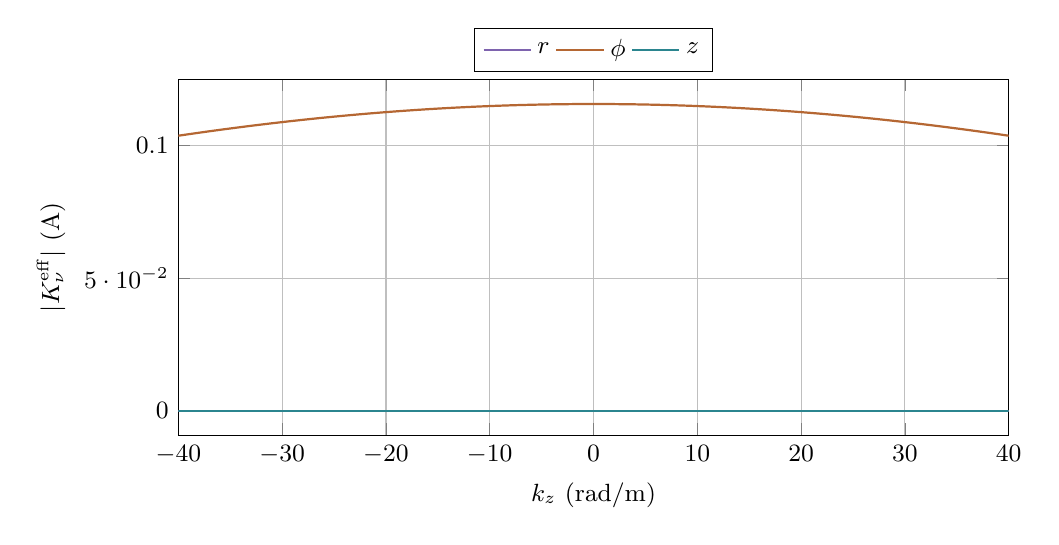
\begin{tikzpicture}
\begin{axis}[width=\linewidth,height=6.1cm,grid=major,
xlabel={$k_z$ (rad/m)},ylabel={$|K^{\rm eff}_\nu|$ (A)},
tick label style={font=\small},label style={font=\small},
legend style={font=\small,at={(.5,1.02)},anchor=south,legend columns=3},
xmin=-40,xmax=40,enlarge y limits=.08]
\addplot[violet,thick,no marks] coordinates {(-40,2.2585518841e-17) (-39,7.16667094869e-17) (-38,4.79709938495e-17) (-37,3.21356357597e-17) (-36,8.30553661592e-17) (-35,1.16242510753e-16) (-34,1.43361072597e-16) (-33,7.02982419773e-17) (-32,8.40664442421e-17) (-31,9.0828855192e-17) (-30,1.32319604593e-16) (-29,1.59382659891e-16) (-28,1.7308104453e-16) (-27,7.42920104588e-17) (-26,6.72959575352e-17) (-25,5.64025727588e-17) (-24,1.01511940282e-16) (-23,1.23215656549e-16) (-22,1.88406594079e-16) (-21,1.01432433952e-16) (-20,7.07438416063e-17) (-19,2.29944794049e-16) (-18,1.35281611818e-16) (-17,9.75323854858e-17) (-16,1.03381671728e-16) (-15,5.80960873124e-17) (-14,2.18590640714e-17) (-13,1.62645561882e-16) (-12,5.97132094366e-17) (-11,5.06911911209e-17) (-10,7.52320728859e-17) (-9,8.01305034655e-17) (-8,1.8630357346e-16) (-7,6.04109866138e-17) (-6,1.71421357557e-16) (-5,1.26631389583e-16) (-4,1.77783604456e-16) (-3,1.20035780498e-16) (-2,1.04314511134e-16) (-1,1.59481273455e-16) (0,2.82001917368e-17) (1,1.68605552493e-16) (2,1.1405619886e-16) (3,1.1481130094e-16) (4,2.35873041121e-16) (5,1.23141125117e-16) (6,1.46982708409e-16) (7,9.87359636321e-17) (8,2.00485127963e-16) (9,5.73258362464e-17) (10,2.09710474819e-17) (11,5.91256777584e-17) (12,1.73990042156e-17) (13,1.50762411532e-16) (14,2.08678320015e-17) (15,8.38173416586e-17) (16,1.04820118954e-16) (17,9.34231000168e-17) (18,7.18512374749e-17) (19,2.22221709706e-16) (20,9.41731132787e-17) (21,9.49995684331e-17) (22,1.6387023178e-16) (23,1.20465799131e-16) (24,1.60094024003e-16) (25,5.40701722582e-17) (26,5.1824565349e-17) (27,7.57119184009e-17) (28,1.57505553469e-16) (29,1.38245406386e-16) (30,1.39243761681e-16) (31,1.00670847626e-16) (32,8.50109806168e-17) (33,6.72196252177e-17) (34,1.49178990458e-16) (35,1.25013172023e-16) (36,9.98505493461e-17) (37,4.91811461871e-17) (38,6.53112844198e-17) (39,7.61797691442e-17) (40,1.17491857905e-17)};
\addlegendentry{$r$}
\addplot[copper,thick,no marks] coordinates {(-40,0.103791607112) (-39,0.104364005539) (-38,0.104923687456) (-37,0.105470520101) (-36,0.10600437368) (-35,0.106525121404) (-34,0.107032639523) (-33,0.107526807366) (-32,0.108007507369) (-31,0.108474625114) (-30,0.108928049358) (-29,0.109367672067) (-28,0.109793388443) (-27,0.11020509696) (-26,0.110602699387) (-25,0.110986100819) (-24,0.111355209704) (-23,0.111709937865) (-22,0.112050200534) (-21,0.112375916367) (-20,0.112687007471) (-19,0.112983399428) (-18,0.113265021312) (-17,0.113531805715) (-16,0.113783688758) (-15,0.114020610118) (-14,0.11424251304) (-13,0.114449344354) (-12,0.11464105449) (-11,0.114817597496) (-10,0.114978931043) (-9,0.115125016446) (-8,0.115255818669) (-7,0.115371306338) (-6,0.115471451748) (-5,0.115556230873) (-4,0.115625623372) (-3,0.115679612591) (-2,0.115718185577) (-1,0.115741333072) (0,0.115749049521) (1,0.115741333072) (2,0.115718185577) (3,0.115679612591) (4,0.115625623372) (5,0.115556230873) (6,0.115471451748) (7,0.115371306338) (8,0.115255818669) (9,0.115125016446) (10,0.114978931043) (11,0.114817597496) (12,0.11464105449) (13,0.114449344354) (14,0.11424251304) (15,0.114020610118) (16,0.113783688758) (17,0.113531805715) (18,0.113265021312) (19,0.112983399428) (20,0.112687007471) (21,0.112375916367) (22,0.112050200534) (23,0.111709937865) (24,0.111355209704) (25,0.110986100819) (26,0.110602699387) (27,0.11020509696) (28,0.109793388443) (29,0.109367672067) (30,0.108928049358) (31,0.108474625114) (32,0.108007507369) (33,0.107526807366) (34,0.107032639523) (35,0.106525121404) (36,0.10600437368) (37,0.105470520101) (38,0.104923687456) (39,0.104364005539) (40,0.103791607112)};
\addlegendentry{$\phi$}
\addplot[teal,thick,no marks] coordinates {(-40,0) (-39,0) (-38,0) (-37,0) (-36,0) (-35,0) (-34,0) (-33,0) (-32,0) (-31,0) (-30,0) (-29,0) (-28,0) (-27,0) (-26,0) (-25,0) (-24,0) (-23,0) (-22,0) (-21,0) (-20,0) (-19,0) (-18,0) (-17,0) (-16,0) (-15,0) (-14,0) (-13,0) (-12,0) (-11,0) (-10,0) (-9,0) (-8,0) (-7,0) (-6,0) (-5,0) (-4,0) (-3,0) (-2,0) (-1,0) (0,0) (1,0) (2,0) (3,0) (4,0) (5,0) (6,0) (7,0) (8,0) (9,0) (10,0) (11,0) (12,0) (13,0) (14,0) (15,0) (16,0) (17,0) (18,0) (19,0) (20,0) (21,0) (22,0) (23,0) (24,0) (25,0) (26,0) (27,0) (28,0) (29,0) (30,0) (31,0) (32,0) (33,0) (34,0) (35,0) (36,0) (37,0) (38,0) (39,0) (40,0)};
\addlegendentry{$z$}
\end{axis}\end{tikzpicture}}
\par\small 展示汇总谱，$m=1$；场加载保留各源半径。
\end{minipage}
% END GENERATED: prescribed_current_14
\end{center}

\subsection{多半径分段环（编号 15）}
给定 $N_r=1,\ldots,8$ 个半径。$N_r>1$ 时
$r_j=a_s+(b-a_s)j/(N_r-1)$，$N_r=1$ 时只用 $r_0=a_s$。
最内环取 $S_0=2$ 段，其他环取 $S_j=4$ 段，与参考文献的分段形式一致。
每段中心、开角及给定电流系数为
\begin{equation}
 \phi_{jh}=\frac{2\pi h}{S_j},\quad
 A_j=\frac{2\pi}{S_j}-g,\quad
 G_{jh}=\begin{cases}\cos(q\phi_{jh}),&\text{余弦驻波},\\
 \ee^{\ii q\phi_{jh}},&\text{旋转相位},\end{cases}
\end{equation}
$h=0,\ldots,S_j-1$；$g$ 是每处间隙角（rad），$0<g<\pi/2$。
$q$ 是\textbf{给定电流的角向谐波}，不同于用于分析输出的 $m$。
每段沿 $+\phi$，承载恒定电流 $IG_{jh}$；各断口允许端点电荷。
程序没有假定文献中的背面接线，也没有将不同段自动连成一条回路。
逐弧积分得到
\begin{equation}\label{eq:segmentedSource}
 \begin{aligned}
 K_r^{\rm eff}&=K_z^{\rm eff}=0,\\
 K_\phi^{\rm eff}&=\frac{CW_z}{2\pi b}
 \sum_{j=0}^{N_r-1}r_j A_j\sinc(mA_j/2)
 \sum_{h=0}^{S_j-1}G_{jh}\ee^{-\ii m\phi_{jh}}.
 \end{aligned}
\end{equation}
每个半径还对应单独的 $\delta(r-r_j)$ 源面。
相位采样、分段数与间隙共同决定输出模式，给定 $q$ 不保证整个源只有 $m=q$。
\begin{center}% BEGIN GENERATED: prescribed_current_15
% Current geometry exported by C; arrows show instantaneous real current at t=0.
\begin{minipage}[t]{.48\linewidth}\centering\vspace{0pt}
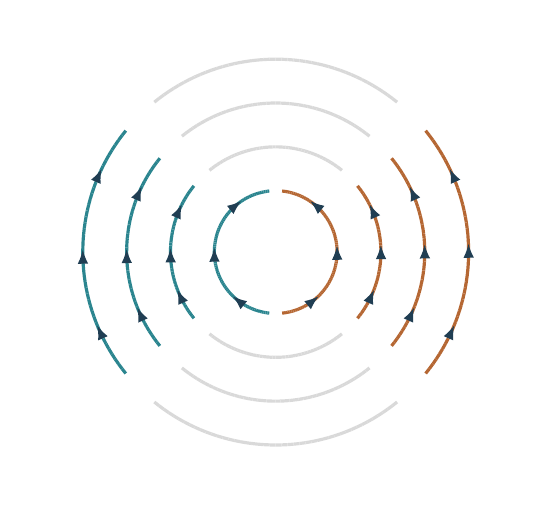
\begin{tikzpicture}[x=1cm,y=1cm,>=Latex,font=\small]
\path[use as bounding box] (-3.15,-2.85) rectangle (3.15,2.85);
\draw[copper,line width=1.15pt] (0.08148,-0.77528)--(0.10562,-0.77236);
\draw[copper,line width=1.15pt] (0.10562,-0.77236)--(0.12966,-0.76869);
\draw[copper,line width=1.15pt] (0.12966,-0.76869)--(0.15357,-0.76427);
\draw[copper,line width=1.15pt] (0.15357,-0.76427)--(0.17733,-0.75911);
\draw[copper,line width=1.15pt] (0.17733,-0.75911)--(0.20092,-0.75321);
\draw[copper,line width=1.15pt] (0.20092,-0.75321)--(0.22432,-0.74657);
\draw[copper,line width=1.15pt] (0.22432,-0.74657)--(0.24749,-0.73922);
\draw[copper,line width=1.15pt] (0.24749,-0.73922)--(0.27042,-0.73114);
\draw[copper,line width=1.15pt] (0.27042,-0.73114)--(0.29310,-0.72235);
\draw[copper,line width=1.15pt] (0.29310,-0.72235)--(0.31548,-0.71285);
\draw[copper,line width=1.15pt] (0.31548,-0.71285)--(0.33756,-0.70267);
\draw[copper,line width=1.15pt] (0.33756,-0.70267)--(0.35931,-0.69180);
\draw[copper,line width=1.15pt] (0.35931,-0.69180)--(0.38071,-0.68026);
\draw[copper,line width=1.15pt] (0.38071,-0.68026)--(0.40174,-0.66805);
\draw[copper,line width=1.15pt] (0.40174,-0.66805)--(0.42238,-0.65520);
\draw[copper,line width=1.15pt] (0.42238,-0.65520)--(0.44261,-0.64171);
\draw[copper,line width=1.15pt] (0.44261,-0.64171)--(0.46241,-0.62759);
\draw[copper,line width=1.15pt] (0.46241,-0.62759)--(0.48176,-0.61286);
\draw[copper,line width=1.15pt] (0.48176,-0.61286)--(0.50064,-0.59754);
\draw[copper,line width=1.15pt] (0.50064,-0.59754)--(0.51903,-0.58163);
\draw[copper,line width=1.15pt] (0.51903,-0.58163)--(0.53692,-0.56516);
\draw[copper,line width=1.15pt] (0.53692,-0.56516)--(0.55428,-0.54814);
\draw[copper,line width=1.15pt] (0.55428,-0.54814)--(0.57111,-0.53059);
\draw[copper,line width=1.15pt] (0.57111,-0.53059)--(0.58738,-0.51252);
\draw[copper,line width=1.15pt] (0.58738,-0.51252)--(0.60308,-0.49395);
\draw[copper,line width=1.15pt] (0.60308,-0.49395)--(0.61819,-0.47490);
\draw[copper,line width=1.15pt] (0.61819,-0.47490)--(0.63270,-0.45539);
\draw[copper,line width=1.15pt] (0.63270,-0.45539)--(0.64660,-0.43544);
\draw[copper,line width=1.15pt] (0.64660,-0.43544)--(0.65986,-0.41506);
\draw[copper,line width=1.15pt] (0.65986,-0.41506)--(0.67249,-0.39428);
\draw[copper,line width=1.15pt] (0.67249,-0.39428)--(0.68446,-0.37311);
\draw[copper,line width=1.15pt] (0.68446,-0.37311)--(0.69576,-0.35158);
\draw[copper,line width=1.15pt] (0.69576,-0.35158)--(0.70639,-0.32971);
\draw[copper,line width=1.15pt] (0.70639,-0.32971)--(0.71633,-0.30752);
\draw[copper,line width=1.15pt] (0.71633,-0.30752)--(0.72557,-0.28503);
\draw[copper,line width=1.15pt] (0.72557,-0.28503)--(0.73410,-0.26226);
\draw[copper,line width=1.15pt] (0.73410,-0.26226)--(0.74193,-0.23924);
\draw[copper,line width=1.15pt] (0.74193,-0.23924)--(0.74903,-0.21598);
\draw[copper,line width=1.15pt] (0.74903,-0.21598)--(0.75540,-0.19252);
\draw[copper,line width=1.15pt] (0.75540,-0.19252)--(0.76104,-0.16887);
\draw[copper,line width=1.15pt] (0.76104,-0.16887)--(0.76593,-0.14505);
\draw[copper,line width=1.15pt] (0.76593,-0.14505)--(0.77008,-0.12109);
\draw[copper,line width=1.15pt] (0.77008,-0.12109)--(0.77349,-0.09701);
\draw[copper,line width=1.15pt] (0.77349,-0.09701)--(0.77613,-0.07284);
\draw[copper,line width=1.15pt] (0.77613,-0.07284)--(0.77803,-0.04860);
\draw[copper,line width=1.15pt] (0.77803,-0.04860)--(0.77917,-0.02431);
\draw[copper,line width=1.15pt] (0.77917,-0.02431)--(0.77955,0.00000);
\draw[copper,line width=1.15pt] (0.77955,0.00000)--(0.77917,0.02431);
\draw[copper,line width=1.15pt] (0.77917,0.02431)--(0.77803,0.04860);
\draw[copper,line width=1.15pt] (0.77803,0.04860)--(0.77613,0.07284);
\draw[copper,line width=1.15pt] (0.77613,0.07284)--(0.77349,0.09701);
\draw[copper,line width=1.15pt] (0.77349,0.09701)--(0.77008,0.12109);
\draw[copper,line width=1.15pt] (0.77008,0.12109)--(0.76593,0.14505);
\draw[copper,line width=1.15pt] (0.76593,0.14505)--(0.76104,0.16887);
\draw[copper,line width=1.15pt] (0.76104,0.16887)--(0.75540,0.19252);
\draw[copper,line width=1.15pt] (0.75540,0.19252)--(0.74903,0.21598);
\draw[copper,line width=1.15pt] (0.74903,0.21598)--(0.74193,0.23924);
\draw[copper,line width=1.15pt] (0.74193,0.23924)--(0.73410,0.26226);
\draw[copper,line width=1.15pt] (0.73410,0.26226)--(0.72557,0.28503);
\draw[copper,line width=1.15pt] (0.72557,0.28503)--(0.71633,0.30752);
\draw[copper,line width=1.15pt] (0.71633,0.30752)--(0.70639,0.32971);
\draw[copper,line width=1.15pt] (0.70639,0.32971)--(0.69576,0.35158);
\draw[copper,line width=1.15pt] (0.69576,0.35158)--(0.68446,0.37311);
\draw[copper,line width=1.15pt] (0.68446,0.37311)--(0.67249,0.39428);
\draw[copper,line width=1.15pt] (0.67249,0.39428)--(0.65986,0.41506);
\draw[copper,line width=1.15pt] (0.65986,0.41506)--(0.64660,0.43544);
\draw[copper,line width=1.15pt] (0.64660,0.43544)--(0.63270,0.45539);
\draw[copper,line width=1.15pt] (0.63270,0.45539)--(0.61819,0.47490);
\draw[copper,line width=1.15pt] (0.61819,0.47490)--(0.60308,0.49395);
\draw[copper,line width=1.15pt] (0.60308,0.49395)--(0.58738,0.51252);
\draw[copper,line width=1.15pt] (0.58738,0.51252)--(0.57111,0.53059);
\draw[copper,line width=1.15pt] (0.57111,0.53059)--(0.55428,0.54814);
\draw[copper,line width=1.15pt] (0.55428,0.54814)--(0.53692,0.56516);
\draw[copper,line width=1.15pt] (0.53692,0.56516)--(0.51903,0.58163);
\draw[copper,line width=1.15pt] (0.51903,0.58163)--(0.50064,0.59754);
\draw[copper,line width=1.15pt] (0.50064,0.59754)--(0.48176,0.61286);
\draw[copper,line width=1.15pt] (0.48176,0.61286)--(0.46241,0.62759);
\draw[copper,line width=1.15pt] (0.46241,0.62759)--(0.44261,0.64171);
\draw[copper,line width=1.15pt] (0.44261,0.64171)--(0.42238,0.65520);
\draw[copper,line width=1.15pt] (0.42238,0.65520)--(0.40174,0.66805);
\draw[copper,line width=1.15pt] (0.40174,0.66805)--(0.38071,0.68026);
\draw[copper,line width=1.15pt] (0.38071,0.68026)--(0.35931,0.69180);
\draw[copper,line width=1.15pt] (0.35931,0.69180)--(0.33756,0.70267);
\draw[copper,line width=1.15pt] (0.33756,0.70267)--(0.31548,0.71285);
\draw[copper,line width=1.15pt] (0.31548,0.71285)--(0.29310,0.72235);
\draw[copper,line width=1.15pt] (0.29310,0.72235)--(0.27042,0.73114);
\draw[copper,line width=1.15pt] (0.27042,0.73114)--(0.24749,0.73922);
\draw[copper,line width=1.15pt] (0.24749,0.73922)--(0.22432,0.74657);
\draw[copper,line width=1.15pt] (0.22432,0.74657)--(0.20092,0.75321);
\draw[copper,line width=1.15pt] (0.20092,0.75321)--(0.17733,0.75911);
\draw[copper,line width=1.15pt] (0.17733,0.75911)--(0.15357,0.76427);
\draw[copper,line width=1.15pt] (0.15357,0.76427)--(0.12966,0.76869);
\draw[copper,line width=1.15pt] (0.12966,0.76869)--(0.10562,0.77236);
\draw[copper,line width=1.15pt] (0.10562,0.77236)--(0.08148,0.77528);
\draw[teal,line width=1.15pt] (-0.08148,0.77528)--(-0.10562,0.77236);
\draw[teal,line width=1.15pt] (-0.10562,0.77236)--(-0.12966,0.76869);
\draw[teal,line width=1.15pt] (-0.12966,0.76869)--(-0.15357,0.76427);
\draw[teal,line width=1.15pt] (-0.15357,0.76427)--(-0.17733,0.75911);
\draw[teal,line width=1.15pt] (-0.17733,0.75911)--(-0.20092,0.75321);
\draw[teal,line width=1.15pt] (-0.20092,0.75321)--(-0.22432,0.74657);
\draw[teal,line width=1.15pt] (-0.22432,0.74657)--(-0.24749,0.73922);
\draw[teal,line width=1.15pt] (-0.24749,0.73922)--(-0.27042,0.73114);
\draw[teal,line width=1.15pt] (-0.27042,0.73114)--(-0.29310,0.72235);
\draw[teal,line width=1.15pt] (-0.29310,0.72235)--(-0.31548,0.71285);
\draw[teal,line width=1.15pt] (-0.31548,0.71285)--(-0.33756,0.70267);
\draw[teal,line width=1.15pt] (-0.33756,0.70267)--(-0.35931,0.69180);
\draw[teal,line width=1.15pt] (-0.35931,0.69180)--(-0.38071,0.68026);
\draw[teal,line width=1.15pt] (-0.38071,0.68026)--(-0.40174,0.66805);
\draw[teal,line width=1.15pt] (-0.40174,0.66805)--(-0.42238,0.65520);
\draw[teal,line width=1.15pt] (-0.42238,0.65520)--(-0.44261,0.64171);
\draw[teal,line width=1.15pt] (-0.44261,0.64171)--(-0.46241,0.62759);
\draw[teal,line width=1.15pt] (-0.46241,0.62759)--(-0.48176,0.61286);
\draw[teal,line width=1.15pt] (-0.48176,0.61286)--(-0.50064,0.59754);
\draw[teal,line width=1.15pt] (-0.50064,0.59754)--(-0.51903,0.58163);
\draw[teal,line width=1.15pt] (-0.51903,0.58163)--(-0.53692,0.56516);
\draw[teal,line width=1.15pt] (-0.53692,0.56516)--(-0.55428,0.54814);
\draw[teal,line width=1.15pt] (-0.55428,0.54814)--(-0.57111,0.53059);
\draw[teal,line width=1.15pt] (-0.57111,0.53059)--(-0.58738,0.51252);
\draw[teal,line width=1.15pt] (-0.58738,0.51252)--(-0.60308,0.49395);
\draw[teal,line width=1.15pt] (-0.60308,0.49395)--(-0.61819,0.47490);
\draw[teal,line width=1.15pt] (-0.61819,0.47490)--(-0.63270,0.45539);
\draw[teal,line width=1.15pt] (-0.63270,0.45539)--(-0.64660,0.43544);
\draw[teal,line width=1.15pt] (-0.64660,0.43544)--(-0.65986,0.41506);
\draw[teal,line width=1.15pt] (-0.65986,0.41506)--(-0.67249,0.39428);
\draw[teal,line width=1.15pt] (-0.67249,0.39428)--(-0.68446,0.37311);
\draw[teal,line width=1.15pt] (-0.68446,0.37311)--(-0.69576,0.35158);
\draw[teal,line width=1.15pt] (-0.69576,0.35158)--(-0.70639,0.32971);
\draw[teal,line width=1.15pt] (-0.70639,0.32971)--(-0.71633,0.30752);
\draw[teal,line width=1.15pt] (-0.71633,0.30752)--(-0.72557,0.28503);
\draw[teal,line width=1.15pt] (-0.72557,0.28503)--(-0.73410,0.26226);
\draw[teal,line width=1.15pt] (-0.73410,0.26226)--(-0.74193,0.23924);
\draw[teal,line width=1.15pt] (-0.74193,0.23924)--(-0.74903,0.21598);
\draw[teal,line width=1.15pt] (-0.74903,0.21598)--(-0.75540,0.19252);
\draw[teal,line width=1.15pt] (-0.75540,0.19252)--(-0.76104,0.16887);
\draw[teal,line width=1.15pt] (-0.76104,0.16887)--(-0.76593,0.14505);
\draw[teal,line width=1.15pt] (-0.76593,0.14505)--(-0.77008,0.12109);
\draw[teal,line width=1.15pt] (-0.77008,0.12109)--(-0.77349,0.09701);
\draw[teal,line width=1.15pt] (-0.77349,0.09701)--(-0.77613,0.07284);
\draw[teal,line width=1.15pt] (-0.77613,0.07284)--(-0.77803,0.04860);
\draw[teal,line width=1.15pt] (-0.77803,0.04860)--(-0.77917,0.02431);
\draw[teal,line width=1.15pt] (-0.77917,0.02431)--(-0.77955,0.00000);
\draw[teal,line width=1.15pt] (-0.77955,0.00000)--(-0.77917,-0.02431);
\draw[teal,line width=1.15pt] (-0.77917,-0.02431)--(-0.77803,-0.04860);
\draw[teal,line width=1.15pt] (-0.77803,-0.04860)--(-0.77613,-0.07284);
\draw[teal,line width=1.15pt] (-0.77613,-0.07284)--(-0.77349,-0.09701);
\draw[teal,line width=1.15pt] (-0.77349,-0.09701)--(-0.77008,-0.12109);
\draw[teal,line width=1.15pt] (-0.77008,-0.12109)--(-0.76593,-0.14505);
\draw[teal,line width=1.15pt] (-0.76593,-0.14505)--(-0.76104,-0.16887);
\draw[teal,line width=1.15pt] (-0.76104,-0.16887)--(-0.75540,-0.19252);
\draw[teal,line width=1.15pt] (-0.75540,-0.19252)--(-0.74903,-0.21598);
\draw[teal,line width=1.15pt] (-0.74903,-0.21598)--(-0.74193,-0.23924);
\draw[teal,line width=1.15pt] (-0.74193,-0.23924)--(-0.73410,-0.26226);
\draw[teal,line width=1.15pt] (-0.73410,-0.26226)--(-0.72557,-0.28503);
\draw[teal,line width=1.15pt] (-0.72557,-0.28503)--(-0.71633,-0.30752);
\draw[teal,line width=1.15pt] (-0.71633,-0.30752)--(-0.70639,-0.32971);
\draw[teal,line width=1.15pt] (-0.70639,-0.32971)--(-0.69576,-0.35158);
\draw[teal,line width=1.15pt] (-0.69576,-0.35158)--(-0.68446,-0.37311);
\draw[teal,line width=1.15pt] (-0.68446,-0.37311)--(-0.67249,-0.39428);
\draw[teal,line width=1.15pt] (-0.67249,-0.39428)--(-0.65986,-0.41506);
\draw[teal,line width=1.15pt] (-0.65986,-0.41506)--(-0.64660,-0.43544);
\draw[teal,line width=1.15pt] (-0.64660,-0.43544)--(-0.63270,-0.45539);
\draw[teal,line width=1.15pt] (-0.63270,-0.45539)--(-0.61819,-0.47490);
\draw[teal,line width=1.15pt] (-0.61819,-0.47490)--(-0.60308,-0.49395);
\draw[teal,line width=1.15pt] (-0.60308,-0.49395)--(-0.58738,-0.51252);
\draw[teal,line width=1.15pt] (-0.58738,-0.51252)--(-0.57111,-0.53059);
\draw[teal,line width=1.15pt] (-0.57111,-0.53059)--(-0.55428,-0.54814);
\draw[teal,line width=1.15pt] (-0.55428,-0.54814)--(-0.53692,-0.56516);
\draw[teal,line width=1.15pt] (-0.53692,-0.56516)--(-0.51903,-0.58163);
\draw[teal,line width=1.15pt] (-0.51903,-0.58163)--(-0.50064,-0.59754);
\draw[teal,line width=1.15pt] (-0.50064,-0.59754)--(-0.48176,-0.61286);
\draw[teal,line width=1.15pt] (-0.48176,-0.61286)--(-0.46241,-0.62759);
\draw[teal,line width=1.15pt] (-0.46241,-0.62759)--(-0.44261,-0.64171);
\draw[teal,line width=1.15pt] (-0.44261,-0.64171)--(-0.42238,-0.65520);
\draw[teal,line width=1.15pt] (-0.42238,-0.65520)--(-0.40174,-0.66805);
\draw[teal,line width=1.15pt] (-0.40174,-0.66805)--(-0.38071,-0.68026);
\draw[teal,line width=1.15pt] (-0.38071,-0.68026)--(-0.35931,-0.69180);
\draw[teal,line width=1.15pt] (-0.35931,-0.69180)--(-0.33756,-0.70267);
\draw[teal,line width=1.15pt] (-0.33756,-0.70267)--(-0.31548,-0.71285);
\draw[teal,line width=1.15pt] (-0.31548,-0.71285)--(-0.29310,-0.72235);
\draw[teal,line width=1.15pt] (-0.29310,-0.72235)--(-0.27042,-0.73114);
\draw[teal,line width=1.15pt] (-0.27042,-0.73114)--(-0.24749,-0.73922);
\draw[teal,line width=1.15pt] (-0.24749,-0.73922)--(-0.22432,-0.74657);
\draw[teal,line width=1.15pt] (-0.22432,-0.74657)--(-0.20092,-0.75321);
\draw[teal,line width=1.15pt] (-0.20092,-0.75321)--(-0.17733,-0.75911);
\draw[teal,line width=1.15pt] (-0.17733,-0.75911)--(-0.15357,-0.76427);
\draw[teal,line width=1.15pt] (-0.15357,-0.76427)--(-0.12966,-0.76869);
\draw[teal,line width=1.15pt] (-0.12966,-0.76869)--(-0.10562,-0.77236);
\draw[teal,line width=1.15pt] (-0.10562,-0.77236)--(-0.08148,-0.77528);
\draw[copper,line width=1.15pt] (1.03855,-0.84100)--(1.06407,-0.80847);
\draw[copper,line width=1.15pt] (1.06407,-0.80847)--(1.08857,-0.77517);
\draw[copper,line width=1.15pt] (1.08857,-0.77517)--(1.11203,-0.74112);
\draw[copper,line width=1.15pt] (1.11203,-0.74112)--(1.13442,-0.70637);
\draw[copper,line width=1.15pt] (1.13442,-0.70637)--(1.15573,-0.67093);
\draw[copper,line width=1.15pt] (1.15573,-0.67093)--(1.17593,-0.63486);
\draw[copper,line width=1.15pt] (1.17593,-0.63486)--(1.19501,-0.59818);
\draw[copper,line width=1.15pt] (1.19501,-0.59818)--(1.21294,-0.56093);
\draw[copper,line width=1.15pt] (1.21294,-0.56093)--(1.22971,-0.52313);
\draw[copper,line width=1.15pt] (1.22971,-0.52313)--(1.24531,-0.48484);
\draw[copper,line width=1.15pt] (1.24531,-0.48484)--(1.25971,-0.44609);
\draw[copper,line width=1.15pt] (1.25971,-0.44609)--(1.27291,-0.40690);
\draw[copper,line width=1.15pt] (1.27291,-0.40690)--(1.28489,-0.36733);
\draw[copper,line width=1.15pt] (1.28489,-0.36733)--(1.29564,-0.32741);
\draw[copper,line width=1.15pt] (1.29564,-0.32741)--(1.30514,-0.28717);
\draw[copper,line width=1.15pt] (1.30514,-0.28717)--(1.31340,-0.24666);
\draw[copper,line width=1.15pt] (1.31340,-0.24666)--(1.32040,-0.20591);
\draw[copper,line width=1.15pt] (1.32040,-0.20591)--(1.32614,-0.16497);
\draw[copper,line width=1.15pt] (1.32614,-0.16497)--(1.33061,-0.12386);
\draw[copper,line width=1.15pt] (1.33061,-0.12386)--(1.33381,-0.08264);
\draw[copper,line width=1.15pt] (1.33381,-0.08264)--(1.33572,-0.04134);
\draw[copper,line width=1.15pt] (1.33572,-0.04134)--(1.33636,0.00000);
\draw[copper,line width=1.15pt] (1.33636,0.00000)--(1.33572,0.04134);
\draw[copper,line width=1.15pt] (1.33572,0.04134)--(1.33381,0.08264);
\draw[copper,line width=1.15pt] (1.33381,0.08264)--(1.33061,0.12386);
\draw[copper,line width=1.15pt] (1.33061,0.12386)--(1.32614,0.16497);
\draw[copper,line width=1.15pt] (1.32614,0.16497)--(1.32040,0.20591);
\draw[copper,line width=1.15pt] (1.32040,0.20591)--(1.31340,0.24666);
\draw[copper,line width=1.15pt] (1.31340,0.24666)--(1.30514,0.28717);
\draw[copper,line width=1.15pt] (1.30514,0.28717)--(1.29564,0.32741);
\draw[copper,line width=1.15pt] (1.29564,0.32741)--(1.28489,0.36733);
\draw[copper,line width=1.15pt] (1.28489,0.36733)--(1.27291,0.40690);
\draw[copper,line width=1.15pt] (1.27291,0.40690)--(1.25971,0.44609);
\draw[copper,line width=1.15pt] (1.25971,0.44609)--(1.24531,0.48484);
\draw[copper,line width=1.15pt] (1.24531,0.48484)--(1.22971,0.52313);
\draw[copper,line width=1.15pt] (1.22971,0.52313)--(1.21294,0.56093);
\draw[copper,line width=1.15pt] (1.21294,0.56093)--(1.19501,0.59818);
\draw[copper,line width=1.15pt] (1.19501,0.59818)--(1.17593,0.63486);
\draw[copper,line width=1.15pt] (1.17593,0.63486)--(1.15573,0.67093);
\draw[copper,line width=1.15pt] (1.15573,0.67093)--(1.13442,0.70637);
\draw[copper,line width=1.15pt] (1.13442,0.70637)--(1.11203,0.74112);
\draw[copper,line width=1.15pt] (1.11203,0.74112)--(1.08857,0.77517);
\draw[copper,line width=1.15pt] (1.08857,0.77517)--(1.06407,0.80847);
\draw[copper,line width=1.15pt] (1.06407,0.80847)--(1.03855,0.84100);
\draw[gray!30,line width=1.15pt] (0.84100,1.03855)--(0.80847,1.06407);
\draw[gray!30,line width=1.15pt] (0.80847,1.06407)--(0.77517,1.08857);
\draw[gray!30,line width=1.15pt] (0.77517,1.08857)--(0.74112,1.11203);
\draw[gray!30,line width=1.15pt] (0.74112,1.11203)--(0.70637,1.13442);
\draw[gray!30,line width=1.15pt] (0.70637,1.13442)--(0.67093,1.15573);
\draw[gray!30,line width=1.15pt] (0.67093,1.15573)--(0.63486,1.17593);
\draw[gray!30,line width=1.15pt] (0.63486,1.17593)--(0.59818,1.19501);
\draw[gray!30,line width=1.15pt] (0.59818,1.19501)--(0.56093,1.21294);
\draw[gray!30,line width=1.15pt] (0.56093,1.21294)--(0.52313,1.22971);
\draw[gray!30,line width=1.15pt] (0.52313,1.22971)--(0.48484,1.24531);
\draw[gray!30,line width=1.15pt] (0.48484,1.24531)--(0.44609,1.25971);
\draw[gray!30,line width=1.15pt] (0.44609,1.25971)--(0.40690,1.27291);
\draw[gray!30,line width=1.15pt] (0.40690,1.27291)--(0.36733,1.28489);
\draw[gray!30,line width=1.15pt] (0.36733,1.28489)--(0.32741,1.29564);
\draw[gray!30,line width=1.15pt] (0.32741,1.29564)--(0.28717,1.30514);
\draw[gray!30,line width=1.15pt] (0.28717,1.30514)--(0.24666,1.31340);
\draw[gray!30,line width=1.15pt] (0.24666,1.31340)--(0.20591,1.32040);
\draw[gray!30,line width=1.15pt] (0.20591,1.32040)--(0.16497,1.32614);
\draw[gray!30,line width=1.15pt] (0.16497,1.32614)--(0.12386,1.33061);
\draw[gray!30,line width=1.15pt] (0.12386,1.33061)--(0.08264,1.33381);
\draw[gray!30,line width=1.15pt] (0.08264,1.33381)--(0.04134,1.33572);
\draw[gray!30,line width=1.15pt] (0.04134,1.33572)--(0.00000,1.33636);
\draw[gray!30,line width=1.15pt] (0.00000,1.33636)--(-0.04134,1.33572);
\draw[gray!30,line width=1.15pt] (-0.04134,1.33572)--(-0.08264,1.33381);
\draw[gray!30,line width=1.15pt] (-0.08264,1.33381)--(-0.12386,1.33061);
\draw[gray!30,line width=1.15pt] (-0.12386,1.33061)--(-0.16497,1.32614);
\draw[gray!30,line width=1.15pt] (-0.16497,1.32614)--(-0.20591,1.32040);
\draw[gray!30,line width=1.15pt] (-0.20591,1.32040)--(-0.24666,1.31340);
\draw[gray!30,line width=1.15pt] (-0.24666,1.31340)--(-0.28717,1.30514);
\draw[gray!30,line width=1.15pt] (-0.28717,1.30514)--(-0.32741,1.29564);
\draw[gray!30,line width=1.15pt] (-0.32741,1.29564)--(-0.36733,1.28489);
\draw[gray!30,line width=1.15pt] (-0.36733,1.28489)--(-0.40690,1.27291);
\draw[gray!30,line width=1.15pt] (-0.40690,1.27291)--(-0.44609,1.25971);
\draw[gray!30,line width=1.15pt] (-0.44609,1.25971)--(-0.48484,1.24531);
\draw[gray!30,line width=1.15pt] (-0.48484,1.24531)--(-0.52313,1.22971);
\draw[gray!30,line width=1.15pt] (-0.52313,1.22971)--(-0.56093,1.21294);
\draw[gray!30,line width=1.15pt] (-0.56093,1.21294)--(-0.59818,1.19501);
\draw[gray!30,line width=1.15pt] (-0.59818,1.19501)--(-0.63486,1.17593);
\draw[gray!30,line width=1.15pt] (-0.63486,1.17593)--(-0.67093,1.15573);
\draw[gray!30,line width=1.15pt] (-0.67093,1.15573)--(-0.70637,1.13442);
\draw[gray!30,line width=1.15pt] (-0.70637,1.13442)--(-0.74112,1.11203);
\draw[gray!30,line width=1.15pt] (-0.74112,1.11203)--(-0.77517,1.08857);
\draw[gray!30,line width=1.15pt] (-0.77517,1.08857)--(-0.80847,1.06407);
\draw[gray!30,line width=1.15pt] (-0.80847,1.06407)--(-0.84100,1.03855);
\draw[teal,line width=1.15pt] (-1.03855,0.84100)--(-1.06407,0.80847);
\draw[teal,line width=1.15pt] (-1.06407,0.80847)--(-1.08857,0.77517);
\draw[teal,line width=1.15pt] (-1.08857,0.77517)--(-1.11203,0.74112);
\draw[teal,line width=1.15pt] (-1.11203,0.74112)--(-1.13442,0.70637);
\draw[teal,line width=1.15pt] (-1.13442,0.70637)--(-1.15573,0.67093);
\draw[teal,line width=1.15pt] (-1.15573,0.67093)--(-1.17593,0.63486);
\draw[teal,line width=1.15pt] (-1.17593,0.63486)--(-1.19501,0.59818);
\draw[teal,line width=1.15pt] (-1.19501,0.59818)--(-1.21294,0.56093);
\draw[teal,line width=1.15pt] (-1.21294,0.56093)--(-1.22971,0.52313);
\draw[teal,line width=1.15pt] (-1.22971,0.52313)--(-1.24531,0.48484);
\draw[teal,line width=1.15pt] (-1.24531,0.48484)--(-1.25971,0.44609);
\draw[teal,line width=1.15pt] (-1.25971,0.44609)--(-1.27291,0.40690);
\draw[teal,line width=1.15pt] (-1.27291,0.40690)--(-1.28489,0.36733);
\draw[teal,line width=1.15pt] (-1.28489,0.36733)--(-1.29564,0.32741);
\draw[teal,line width=1.15pt] (-1.29564,0.32741)--(-1.30514,0.28717);
\draw[teal,line width=1.15pt] (-1.30514,0.28717)--(-1.31340,0.24666);
\draw[teal,line width=1.15pt] (-1.31340,0.24666)--(-1.32040,0.20591);
\draw[teal,line width=1.15pt] (-1.32040,0.20591)--(-1.32614,0.16497);
\draw[teal,line width=1.15pt] (-1.32614,0.16497)--(-1.33061,0.12386);
\draw[teal,line width=1.15pt] (-1.33061,0.12386)--(-1.33381,0.08264);
\draw[teal,line width=1.15pt] (-1.33381,0.08264)--(-1.33572,0.04134);
\draw[teal,line width=1.15pt] (-1.33572,0.04134)--(-1.33636,0.00000);
\draw[teal,line width=1.15pt] (-1.33636,0.00000)--(-1.33572,-0.04134);
\draw[teal,line width=1.15pt] (-1.33572,-0.04134)--(-1.33381,-0.08264);
\draw[teal,line width=1.15pt] (-1.33381,-0.08264)--(-1.33061,-0.12386);
\draw[teal,line width=1.15pt] (-1.33061,-0.12386)--(-1.32614,-0.16497);
\draw[teal,line width=1.15pt] (-1.32614,-0.16497)--(-1.32040,-0.20591);
\draw[teal,line width=1.15pt] (-1.32040,-0.20591)--(-1.31340,-0.24666);
\draw[teal,line width=1.15pt] (-1.31340,-0.24666)--(-1.30514,-0.28717);
\draw[teal,line width=1.15pt] (-1.30514,-0.28717)--(-1.29564,-0.32741);
\draw[teal,line width=1.15pt] (-1.29564,-0.32741)--(-1.28489,-0.36733);
\draw[teal,line width=1.15pt] (-1.28489,-0.36733)--(-1.27291,-0.40690);
\draw[teal,line width=1.15pt] (-1.27291,-0.40690)--(-1.25971,-0.44609);
\draw[teal,line width=1.15pt] (-1.25971,-0.44609)--(-1.24531,-0.48484);
\draw[teal,line width=1.15pt] (-1.24531,-0.48484)--(-1.22971,-0.52313);
\draw[teal,line width=1.15pt] (-1.22971,-0.52313)--(-1.21294,-0.56093);
\draw[teal,line width=1.15pt] (-1.21294,-0.56093)--(-1.19501,-0.59818);
\draw[teal,line width=1.15pt] (-1.19501,-0.59818)--(-1.17593,-0.63486);
\draw[teal,line width=1.15pt] (-1.17593,-0.63486)--(-1.15573,-0.67093);
\draw[teal,line width=1.15pt] (-1.15573,-0.67093)--(-1.13442,-0.70637);
\draw[teal,line width=1.15pt] (-1.13442,-0.70637)--(-1.11203,-0.74112);
\draw[teal,line width=1.15pt] (-1.11203,-0.74112)--(-1.08857,-0.77517);
\draw[teal,line width=1.15pt] (-1.08857,-0.77517)--(-1.06407,-0.80847);
\draw[teal,line width=1.15pt] (-1.06407,-0.80847)--(-1.03855,-0.84100);
\draw[gray!30,line width=1.15pt] (-0.84100,-1.03855)--(-0.80847,-1.06407);
\draw[gray!30,line width=1.15pt] (-0.80847,-1.06407)--(-0.77517,-1.08857);
\draw[gray!30,line width=1.15pt] (-0.77517,-1.08857)--(-0.74112,-1.11203);
\draw[gray!30,line width=1.15pt] (-0.74112,-1.11203)--(-0.70637,-1.13442);
\draw[gray!30,line width=1.15pt] (-0.70637,-1.13442)--(-0.67093,-1.15573);
\draw[gray!30,line width=1.15pt] (-0.67093,-1.15573)--(-0.63486,-1.17593);
\draw[gray!30,line width=1.15pt] (-0.63486,-1.17593)--(-0.59818,-1.19501);
\draw[gray!30,line width=1.15pt] (-0.59818,-1.19501)--(-0.56093,-1.21294);
\draw[gray!30,line width=1.15pt] (-0.56093,-1.21294)--(-0.52313,-1.22971);
\draw[gray!30,line width=1.15pt] (-0.52313,-1.22971)--(-0.48484,-1.24531);
\draw[gray!30,line width=1.15pt] (-0.48484,-1.24531)--(-0.44609,-1.25971);
\draw[gray!30,line width=1.15pt] (-0.44609,-1.25971)--(-0.40690,-1.27291);
\draw[gray!30,line width=1.15pt] (-0.40690,-1.27291)--(-0.36733,-1.28489);
\draw[gray!30,line width=1.15pt] (-0.36733,-1.28489)--(-0.32741,-1.29564);
\draw[gray!30,line width=1.15pt] (-0.32741,-1.29564)--(-0.28717,-1.30514);
\draw[gray!30,line width=1.15pt] (-0.28717,-1.30514)--(-0.24666,-1.31340);
\draw[gray!30,line width=1.15pt] (-0.24666,-1.31340)--(-0.20591,-1.32040);
\draw[gray!30,line width=1.15pt] (-0.20591,-1.32040)--(-0.16497,-1.32614);
\draw[gray!30,line width=1.15pt] (-0.16497,-1.32614)--(-0.12386,-1.33061);
\draw[gray!30,line width=1.15pt] (-0.12386,-1.33061)--(-0.08264,-1.33381);
\draw[gray!30,line width=1.15pt] (-0.08264,-1.33381)--(-0.04134,-1.33572);
\draw[gray!30,line width=1.15pt] (-0.04134,-1.33572)--(-0.00000,-1.33636);
\draw[gray!30,line width=1.15pt] (-0.00000,-1.33636)--(0.04134,-1.33572);
\draw[gray!30,line width=1.15pt] (0.04134,-1.33572)--(0.08264,-1.33381);
\draw[gray!30,line width=1.15pt] (0.08264,-1.33381)--(0.12386,-1.33061);
\draw[gray!30,line width=1.15pt] (0.12386,-1.33061)--(0.16497,-1.32614);
\draw[gray!30,line width=1.15pt] (0.16497,-1.32614)--(0.20591,-1.32040);
\draw[gray!30,line width=1.15pt] (0.20591,-1.32040)--(0.24666,-1.31340);
\draw[gray!30,line width=1.15pt] (0.24666,-1.31340)--(0.28717,-1.30514);
\draw[gray!30,line width=1.15pt] (0.28717,-1.30514)--(0.32741,-1.29564);
\draw[gray!30,line width=1.15pt] (0.32741,-1.29564)--(0.36733,-1.28489);
\draw[gray!30,line width=1.15pt] (0.36733,-1.28489)--(0.40690,-1.27291);
\draw[gray!30,line width=1.15pt] (0.40690,-1.27291)--(0.44609,-1.25971);
\draw[gray!30,line width=1.15pt] (0.44609,-1.25971)--(0.48484,-1.24531);
\draw[gray!30,line width=1.15pt] (0.48484,-1.24531)--(0.52313,-1.22971);
\draw[gray!30,line width=1.15pt] (0.52313,-1.22971)--(0.56093,-1.21294);
\draw[gray!30,line width=1.15pt] (0.56093,-1.21294)--(0.59818,-1.19501);
\draw[gray!30,line width=1.15pt] (0.59818,-1.19501)--(0.63486,-1.17593);
\draw[gray!30,line width=1.15pt] (0.63486,-1.17593)--(0.67093,-1.15573);
\draw[gray!30,line width=1.15pt] (0.67093,-1.15573)--(0.70637,-1.13442);
\draw[gray!30,line width=1.15pt] (0.70637,-1.13442)--(0.74112,-1.11203);
\draw[gray!30,line width=1.15pt] (0.74112,-1.11203)--(0.77517,-1.08857);
\draw[gray!30,line width=1.15pt] (0.77517,-1.08857)--(0.80847,-1.06407);
\draw[gray!30,line width=1.15pt] (0.80847,-1.06407)--(0.84100,-1.03855);
\draw[copper,line width=1.15pt] (1.47128,-1.19142)--(1.50743,-1.14533);
\draw[copper,line width=1.15pt] (1.50743,-1.14533)--(1.54214,-1.09815);
\draw[copper,line width=1.15pt] (1.54214,-1.09815)--(1.57537,-1.04992);
\draw[copper,line width=1.15pt] (1.57537,-1.04992)--(1.60710,-1.00068);
\draw[copper,line width=1.15pt] (1.60710,-1.00068)--(1.63729,-0.95049);
\draw[copper,line width=1.15pt] (1.63729,-0.95049)--(1.66591,-0.89939);
\draw[copper,line width=1.15pt] (1.66591,-0.89939)--(1.69293,-0.84742);
\draw[copper,line width=1.15pt] (1.69293,-0.84742)--(1.71834,-0.79464);
\draw[copper,line width=1.15pt] (1.71834,-0.79464)--(1.74210,-0.74111);
\draw[copper,line width=1.15pt] (1.74210,-0.74111)--(1.76419,-0.68686);
\draw[copper,line width=1.15pt] (1.76419,-0.68686)--(1.78459,-0.63196);
\draw[copper,line width=1.15pt] (1.78459,-0.63196)--(1.80329,-0.57645);
\draw[copper,line width=1.15pt] (1.80329,-0.57645)--(1.82026,-0.52039);
\draw[copper,line width=1.15pt] (1.82026,-0.52039)--(1.83548,-0.46383);
\draw[copper,line width=1.15pt] (1.83548,-0.46383)--(1.84895,-0.40683);
\draw[copper,line width=1.15pt] (1.84895,-0.40683)--(1.86065,-0.34943);
\draw[copper,line width=1.15pt] (1.86065,-0.34943)--(1.87057,-0.29171);
\draw[copper,line width=1.15pt] (1.87057,-0.29171)--(1.87870,-0.23370);
\draw[copper,line width=1.15pt] (1.87870,-0.23370)--(1.88503,-0.17547);
\draw[copper,line width=1.15pt] (1.88503,-0.17547)--(1.88956,-0.11708);
\draw[copper,line width=1.15pt] (1.88956,-0.11708)--(1.89228,-0.05857);
\draw[copper,line width=1.15pt] (1.89228,-0.05857)--(1.89318,0.00000);
\draw[copper,line width=1.15pt] (1.89318,0.00000)--(1.89228,0.05857);
\draw[copper,line width=1.15pt] (1.89228,0.05857)--(1.88956,0.11708);
\draw[copper,line width=1.15pt] (1.88956,0.11708)--(1.88503,0.17547);
\draw[copper,line width=1.15pt] (1.88503,0.17547)--(1.87870,0.23370);
\draw[copper,line width=1.15pt] (1.87870,0.23370)--(1.87057,0.29171);
\draw[copper,line width=1.15pt] (1.87057,0.29171)--(1.86065,0.34943);
\draw[copper,line width=1.15pt] (1.86065,0.34943)--(1.84895,0.40683);
\draw[copper,line width=1.15pt] (1.84895,0.40683)--(1.83548,0.46383);
\draw[copper,line width=1.15pt] (1.83548,0.46383)--(1.82026,0.52039);
\draw[copper,line width=1.15pt] (1.82026,0.52039)--(1.80329,0.57645);
\draw[copper,line width=1.15pt] (1.80329,0.57645)--(1.78459,0.63196);
\draw[copper,line width=1.15pt] (1.78459,0.63196)--(1.76419,0.68686);
\draw[copper,line width=1.15pt] (1.76419,0.68686)--(1.74210,0.74111);
\draw[copper,line width=1.15pt] (1.74210,0.74111)--(1.71834,0.79464);
\draw[copper,line width=1.15pt] (1.71834,0.79464)--(1.69293,0.84742);
\draw[copper,line width=1.15pt] (1.69293,0.84742)--(1.66591,0.89939);
\draw[copper,line width=1.15pt] (1.66591,0.89939)--(1.63729,0.95049);
\draw[copper,line width=1.15pt] (1.63729,0.95049)--(1.60710,1.00068);
\draw[copper,line width=1.15pt] (1.60710,1.00068)--(1.57537,1.04992);
\draw[copper,line width=1.15pt] (1.57537,1.04992)--(1.54214,1.09815);
\draw[copper,line width=1.15pt] (1.54214,1.09815)--(1.50743,1.14533);
\draw[copper,line width=1.15pt] (1.50743,1.14533)--(1.47128,1.19142);
\draw[gray!30,line width=1.15pt] (1.19142,1.47128)--(1.14533,1.50743);
\draw[gray!30,line width=1.15pt] (1.14533,1.50743)--(1.09815,1.54214);
\draw[gray!30,line width=1.15pt] (1.09815,1.54214)--(1.04992,1.57537);
\draw[gray!30,line width=1.15pt] (1.04992,1.57537)--(1.00068,1.60710);
\draw[gray!30,line width=1.15pt] (1.00068,1.60710)--(0.95049,1.63729);
\draw[gray!30,line width=1.15pt] (0.95049,1.63729)--(0.89939,1.66591);
\draw[gray!30,line width=1.15pt] (0.89939,1.66591)--(0.84742,1.69293);
\draw[gray!30,line width=1.15pt] (0.84742,1.69293)--(0.79464,1.71834);
\draw[gray!30,line width=1.15pt] (0.79464,1.71834)--(0.74111,1.74210);
\draw[gray!30,line width=1.15pt] (0.74111,1.74210)--(0.68686,1.76419);
\draw[gray!30,line width=1.15pt] (0.68686,1.76419)--(0.63196,1.78459);
\draw[gray!30,line width=1.15pt] (0.63196,1.78459)--(0.57645,1.80329);
\draw[gray!30,line width=1.15pt] (0.57645,1.80329)--(0.52039,1.82026);
\draw[gray!30,line width=1.15pt] (0.52039,1.82026)--(0.46383,1.83548);
\draw[gray!30,line width=1.15pt] (0.46383,1.83548)--(0.40683,1.84895);
\draw[gray!30,line width=1.15pt] (0.40683,1.84895)--(0.34943,1.86065);
\draw[gray!30,line width=1.15pt] (0.34943,1.86065)--(0.29171,1.87057);
\draw[gray!30,line width=1.15pt] (0.29171,1.87057)--(0.23370,1.87870);
\draw[gray!30,line width=1.15pt] (0.23370,1.87870)--(0.17547,1.88503);
\draw[gray!30,line width=1.15pt] (0.17547,1.88503)--(0.11708,1.88956);
\draw[gray!30,line width=1.15pt] (0.11708,1.88956)--(0.05857,1.89228);
\draw[gray!30,line width=1.15pt] (0.05857,1.89228)--(0.00000,1.89318);
\draw[gray!30,line width=1.15pt] (0.00000,1.89318)--(-0.05857,1.89228);
\draw[gray!30,line width=1.15pt] (-0.05857,1.89228)--(-0.11708,1.88956);
\draw[gray!30,line width=1.15pt] (-0.11708,1.88956)--(-0.17547,1.88503);
\draw[gray!30,line width=1.15pt] (-0.17547,1.88503)--(-0.23370,1.87870);
\draw[gray!30,line width=1.15pt] (-0.23370,1.87870)--(-0.29171,1.87057);
\draw[gray!30,line width=1.15pt] (-0.29171,1.87057)--(-0.34943,1.86065);
\draw[gray!30,line width=1.15pt] (-0.34943,1.86065)--(-0.40683,1.84895);
\draw[gray!30,line width=1.15pt] (-0.40683,1.84895)--(-0.46383,1.83548);
\draw[gray!30,line width=1.15pt] (-0.46383,1.83548)--(-0.52039,1.82026);
\draw[gray!30,line width=1.15pt] (-0.52039,1.82026)--(-0.57645,1.80329);
\draw[gray!30,line width=1.15pt] (-0.57645,1.80329)--(-0.63196,1.78459);
\draw[gray!30,line width=1.15pt] (-0.63196,1.78459)--(-0.68686,1.76419);
\draw[gray!30,line width=1.15pt] (-0.68686,1.76419)--(-0.74111,1.74210);
\draw[gray!30,line width=1.15pt] (-0.74111,1.74210)--(-0.79464,1.71834);
\draw[gray!30,line width=1.15pt] (-0.79464,1.71834)--(-0.84742,1.69293);
\draw[gray!30,line width=1.15pt] (-0.84742,1.69293)--(-0.89939,1.66591);
\draw[gray!30,line width=1.15pt] (-0.89939,1.66591)--(-0.95049,1.63729);
\draw[gray!30,line width=1.15pt] (-0.95049,1.63729)--(-1.00068,1.60710);
\draw[gray!30,line width=1.15pt] (-1.00068,1.60710)--(-1.04992,1.57537);
\draw[gray!30,line width=1.15pt] (-1.04992,1.57537)--(-1.09815,1.54214);
\draw[gray!30,line width=1.15pt] (-1.09815,1.54214)--(-1.14533,1.50743);
\draw[gray!30,line width=1.15pt] (-1.14533,1.50743)--(-1.19142,1.47128);
\draw[teal,line width=1.15pt] (-1.47128,1.19142)--(-1.50743,1.14533);
\draw[teal,line width=1.15pt] (-1.50743,1.14533)--(-1.54214,1.09815);
\draw[teal,line width=1.15pt] (-1.54214,1.09815)--(-1.57537,1.04992);
\draw[teal,line width=1.15pt] (-1.57537,1.04992)--(-1.60710,1.00068);
\draw[teal,line width=1.15pt] (-1.60710,1.00068)--(-1.63729,0.95049);
\draw[teal,line width=1.15pt] (-1.63729,0.95049)--(-1.66591,0.89939);
\draw[teal,line width=1.15pt] (-1.66591,0.89939)--(-1.69293,0.84742);
\draw[teal,line width=1.15pt] (-1.69293,0.84742)--(-1.71834,0.79464);
\draw[teal,line width=1.15pt] (-1.71834,0.79464)--(-1.74210,0.74111);
\draw[teal,line width=1.15pt] (-1.74210,0.74111)--(-1.76419,0.68686);
\draw[teal,line width=1.15pt] (-1.76419,0.68686)--(-1.78459,0.63196);
\draw[teal,line width=1.15pt] (-1.78459,0.63196)--(-1.80329,0.57645);
\draw[teal,line width=1.15pt] (-1.80329,0.57645)--(-1.82026,0.52039);
\draw[teal,line width=1.15pt] (-1.82026,0.52039)--(-1.83548,0.46383);
\draw[teal,line width=1.15pt] (-1.83548,0.46383)--(-1.84895,0.40683);
\draw[teal,line width=1.15pt] (-1.84895,0.40683)--(-1.86065,0.34943);
\draw[teal,line width=1.15pt] (-1.86065,0.34943)--(-1.87057,0.29171);
\draw[teal,line width=1.15pt] (-1.87057,0.29171)--(-1.87870,0.23370);
\draw[teal,line width=1.15pt] (-1.87870,0.23370)--(-1.88503,0.17547);
\draw[teal,line width=1.15pt] (-1.88503,0.17547)--(-1.88956,0.11708);
\draw[teal,line width=1.15pt] (-1.88956,0.11708)--(-1.89228,0.05857);
\draw[teal,line width=1.15pt] (-1.89228,0.05857)--(-1.89318,0.00000);
\draw[teal,line width=1.15pt] (-1.89318,0.00000)--(-1.89228,-0.05857);
\draw[teal,line width=1.15pt] (-1.89228,-0.05857)--(-1.88956,-0.11708);
\draw[teal,line width=1.15pt] (-1.88956,-0.11708)--(-1.88503,-0.17547);
\draw[teal,line width=1.15pt] (-1.88503,-0.17547)--(-1.87870,-0.23370);
\draw[teal,line width=1.15pt] (-1.87870,-0.23370)--(-1.87057,-0.29171);
\draw[teal,line width=1.15pt] (-1.87057,-0.29171)--(-1.86065,-0.34943);
\draw[teal,line width=1.15pt] (-1.86065,-0.34943)--(-1.84895,-0.40683);
\draw[teal,line width=1.15pt] (-1.84895,-0.40683)--(-1.83548,-0.46383);
\draw[teal,line width=1.15pt] (-1.83548,-0.46383)--(-1.82026,-0.52039);
\draw[teal,line width=1.15pt] (-1.82026,-0.52039)--(-1.80329,-0.57645);
\draw[teal,line width=1.15pt] (-1.80329,-0.57645)--(-1.78459,-0.63196);
\draw[teal,line width=1.15pt] (-1.78459,-0.63196)--(-1.76419,-0.68686);
\draw[teal,line width=1.15pt] (-1.76419,-0.68686)--(-1.74210,-0.74111);
\draw[teal,line width=1.15pt] (-1.74210,-0.74111)--(-1.71834,-0.79464);
\draw[teal,line width=1.15pt] (-1.71834,-0.79464)--(-1.69293,-0.84742);
\draw[teal,line width=1.15pt] (-1.69293,-0.84742)--(-1.66591,-0.89939);
\draw[teal,line width=1.15pt] (-1.66591,-0.89939)--(-1.63729,-0.95049);
\draw[teal,line width=1.15pt] (-1.63729,-0.95049)--(-1.60710,-1.00068);
\draw[teal,line width=1.15pt] (-1.60710,-1.00068)--(-1.57537,-1.04992);
\draw[teal,line width=1.15pt] (-1.57537,-1.04992)--(-1.54214,-1.09815);
\draw[teal,line width=1.15pt] (-1.54214,-1.09815)--(-1.50743,-1.14533);
\draw[teal,line width=1.15pt] (-1.50743,-1.14533)--(-1.47128,-1.19142);
\draw[gray!30,line width=1.15pt] (-1.19142,-1.47128)--(-1.14533,-1.50743);
\draw[gray!30,line width=1.15pt] (-1.14533,-1.50743)--(-1.09815,-1.54214);
\draw[gray!30,line width=1.15pt] (-1.09815,-1.54214)--(-1.04992,-1.57537);
\draw[gray!30,line width=1.15pt] (-1.04992,-1.57537)--(-1.00068,-1.60710);
\draw[gray!30,line width=1.15pt] (-1.00068,-1.60710)--(-0.95049,-1.63729);
\draw[gray!30,line width=1.15pt] (-0.95049,-1.63729)--(-0.89939,-1.66591);
\draw[gray!30,line width=1.15pt] (-0.89939,-1.66591)--(-0.84742,-1.69293);
\draw[gray!30,line width=1.15pt] (-0.84742,-1.69293)--(-0.79464,-1.71834);
\draw[gray!30,line width=1.15pt] (-0.79464,-1.71834)--(-0.74111,-1.74210);
\draw[gray!30,line width=1.15pt] (-0.74111,-1.74210)--(-0.68686,-1.76419);
\draw[gray!30,line width=1.15pt] (-0.68686,-1.76419)--(-0.63196,-1.78459);
\draw[gray!30,line width=1.15pt] (-0.63196,-1.78459)--(-0.57645,-1.80329);
\draw[gray!30,line width=1.15pt] (-0.57645,-1.80329)--(-0.52039,-1.82026);
\draw[gray!30,line width=1.15pt] (-0.52039,-1.82026)--(-0.46383,-1.83548);
\draw[gray!30,line width=1.15pt] (-0.46383,-1.83548)--(-0.40683,-1.84895);
\draw[gray!30,line width=1.15pt] (-0.40683,-1.84895)--(-0.34943,-1.86065);
\draw[gray!30,line width=1.15pt] (-0.34943,-1.86065)--(-0.29171,-1.87057);
\draw[gray!30,line width=1.15pt] (-0.29171,-1.87057)--(-0.23370,-1.87870);
\draw[gray!30,line width=1.15pt] (-0.23370,-1.87870)--(-0.17547,-1.88503);
\draw[gray!30,line width=1.15pt] (-0.17547,-1.88503)--(-0.11708,-1.88956);
\draw[gray!30,line width=1.15pt] (-0.11708,-1.88956)--(-0.05857,-1.89228);
\draw[gray!30,line width=1.15pt] (-0.05857,-1.89228)--(-0.00000,-1.89318);
\draw[gray!30,line width=1.15pt] (-0.00000,-1.89318)--(0.05857,-1.89228);
\draw[gray!30,line width=1.15pt] (0.05857,-1.89228)--(0.11708,-1.88956);
\draw[gray!30,line width=1.15pt] (0.11708,-1.88956)--(0.17547,-1.88503);
\draw[gray!30,line width=1.15pt] (0.17547,-1.88503)--(0.23370,-1.87870);
\draw[gray!30,line width=1.15pt] (0.23370,-1.87870)--(0.29171,-1.87057);
\draw[gray!30,line width=1.15pt] (0.29171,-1.87057)--(0.34943,-1.86065);
\draw[gray!30,line width=1.15pt] (0.34943,-1.86065)--(0.40683,-1.84895);
\draw[gray!30,line width=1.15pt] (0.40683,-1.84895)--(0.46383,-1.83548);
\draw[gray!30,line width=1.15pt] (0.46383,-1.83548)--(0.52039,-1.82026);
\draw[gray!30,line width=1.15pt] (0.52039,-1.82026)--(0.57645,-1.80329);
\draw[gray!30,line width=1.15pt] (0.57645,-1.80329)--(0.63196,-1.78459);
\draw[gray!30,line width=1.15pt] (0.63196,-1.78459)--(0.68686,-1.76419);
\draw[gray!30,line width=1.15pt] (0.68686,-1.76419)--(0.74111,-1.74210);
\draw[gray!30,line width=1.15pt] (0.74111,-1.74210)--(0.79464,-1.71834);
\draw[gray!30,line width=1.15pt] (0.79464,-1.71834)--(0.84742,-1.69293);
\draw[gray!30,line width=1.15pt] (0.84742,-1.69293)--(0.89939,-1.66591);
\draw[gray!30,line width=1.15pt] (0.89939,-1.66591)--(0.95049,-1.63729);
\draw[gray!30,line width=1.15pt] (0.95049,-1.63729)--(1.00068,-1.60710);
\draw[gray!30,line width=1.15pt] (1.00068,-1.60710)--(1.04992,-1.57537);
\draw[gray!30,line width=1.15pt] (1.04992,-1.57537)--(1.09815,-1.54214);
\draw[gray!30,line width=1.15pt] (1.09815,-1.54214)--(1.14533,-1.50743);
\draw[gray!30,line width=1.15pt] (1.14533,-1.50743)--(1.19142,-1.47128);
\draw[copper,line width=1.15pt] (1.90401,-1.54183)--(1.95079,-1.48220);
\draw[copper,line width=1.15pt] (1.95079,-1.48220)--(1.99571,-1.42114);
\draw[copper,line width=1.15pt] (1.99571,-1.42114)--(2.03872,-1.35872);
\draw[copper,line width=1.15pt] (2.03872,-1.35872)--(2.07978,-1.29500);
\draw[copper,line width=1.15pt] (2.07978,-1.29500)--(2.11884,-1.23005);
\draw[copper,line width=1.15pt] (2.11884,-1.23005)--(2.15588,-1.16391);
\draw[copper,line width=1.15pt] (2.15588,-1.16391)--(2.19085,-1.09666);
\draw[copper,line width=1.15pt] (2.19085,-1.09666)--(2.22373,-1.02836);
\draw[copper,line width=1.15pt] (2.22373,-1.02836)--(2.25448,-0.95908);
\draw[copper,line width=1.15pt] (2.25448,-0.95908)--(2.28307,-0.88888);
\draw[copper,line width=1.15pt] (2.28307,-0.88888)--(2.30947,-0.81783);
\draw[copper,line width=1.15pt] (2.30947,-0.81783)--(2.33367,-0.74599);
\draw[copper,line width=1.15pt] (2.33367,-0.74599)--(2.35563,-0.67344);
\draw[copper,line width=1.15pt] (2.35563,-0.67344)--(2.37533,-0.60025);
\draw[copper,line width=1.15pt] (2.37533,-0.60025)--(2.39276,-0.52648);
\draw[copper,line width=1.15pt] (2.39276,-0.52648)--(2.40791,-0.45221);
\draw[copper,line width=1.15pt] (2.40791,-0.45221)--(2.42074,-0.37750);
\draw[copper,line width=1.15pt] (2.42074,-0.37750)--(2.43126,-0.30244);
\draw[copper,line width=1.15pt] (2.43126,-0.30244)--(2.43945,-0.22708);
\draw[copper,line width=1.15pt] (2.43945,-0.22708)--(2.44531,-0.15151);
\draw[copper,line width=1.15pt] (2.44531,-0.15151)--(2.44883,-0.07579);
\draw[copper,line width=1.15pt] (2.44883,-0.07579)--(2.45000,0.00000);
\draw[copper,line width=1.15pt] (2.45000,0.00000)--(2.44883,0.07579);
\draw[copper,line width=1.15pt] (2.44883,0.07579)--(2.44531,0.15151);
\draw[copper,line width=1.15pt] (2.44531,0.15151)--(2.43945,0.22708);
\draw[copper,line width=1.15pt] (2.43945,0.22708)--(2.43126,0.30244);
\draw[copper,line width=1.15pt] (2.43126,0.30244)--(2.42074,0.37750);
\draw[copper,line width=1.15pt] (2.42074,0.37750)--(2.40791,0.45221);
\draw[copper,line width=1.15pt] (2.40791,0.45221)--(2.39276,0.52648);
\draw[copper,line width=1.15pt] (2.39276,0.52648)--(2.37533,0.60025);
\draw[copper,line width=1.15pt] (2.37533,0.60025)--(2.35563,0.67344);
\draw[copper,line width=1.15pt] (2.35563,0.67344)--(2.33367,0.74599);
\draw[copper,line width=1.15pt] (2.33367,0.74599)--(2.30947,0.81783);
\draw[copper,line width=1.15pt] (2.30947,0.81783)--(2.28307,0.88888);
\draw[copper,line width=1.15pt] (2.28307,0.88888)--(2.25448,0.95908);
\draw[copper,line width=1.15pt] (2.25448,0.95908)--(2.22373,1.02836);
\draw[copper,line width=1.15pt] (2.22373,1.02836)--(2.19085,1.09666);
\draw[copper,line width=1.15pt] (2.19085,1.09666)--(2.15588,1.16391);
\draw[copper,line width=1.15pt] (2.15588,1.16391)--(2.11884,1.23005);
\draw[copper,line width=1.15pt] (2.11884,1.23005)--(2.07978,1.29500);
\draw[copper,line width=1.15pt] (2.07978,1.29500)--(2.03872,1.35872);
\draw[copper,line width=1.15pt] (2.03872,1.35872)--(1.99571,1.42114);
\draw[copper,line width=1.15pt] (1.99571,1.42114)--(1.95079,1.48220);
\draw[copper,line width=1.15pt] (1.95079,1.48220)--(1.90401,1.54183);
\draw[gray!30,line width=1.15pt] (1.54183,1.90401)--(1.48220,1.95079);
\draw[gray!30,line width=1.15pt] (1.48220,1.95079)--(1.42114,1.99571);
\draw[gray!30,line width=1.15pt] (1.42114,1.99571)--(1.35872,2.03872);
\draw[gray!30,line width=1.15pt] (1.35872,2.03872)--(1.29500,2.07978);
\draw[gray!30,line width=1.15pt] (1.29500,2.07978)--(1.23005,2.11884);
\draw[gray!30,line width=1.15pt] (1.23005,2.11884)--(1.16391,2.15588);
\draw[gray!30,line width=1.15pt] (1.16391,2.15588)--(1.09666,2.19085);
\draw[gray!30,line width=1.15pt] (1.09666,2.19085)--(1.02836,2.22373);
\draw[gray!30,line width=1.15pt] (1.02836,2.22373)--(0.95908,2.25448);
\draw[gray!30,line width=1.15pt] (0.95908,2.25448)--(0.88888,2.28307);
\draw[gray!30,line width=1.15pt] (0.88888,2.28307)--(0.81783,2.30947);
\draw[gray!30,line width=1.15pt] (0.81783,2.30947)--(0.74599,2.33367);
\draw[gray!30,line width=1.15pt] (0.74599,2.33367)--(0.67344,2.35563);
\draw[gray!30,line width=1.15pt] (0.67344,2.35563)--(0.60025,2.37533);
\draw[gray!30,line width=1.15pt] (0.60025,2.37533)--(0.52648,2.39276);
\draw[gray!30,line width=1.15pt] (0.52648,2.39276)--(0.45221,2.40791);
\draw[gray!30,line width=1.15pt] (0.45221,2.40791)--(0.37750,2.42074);
\draw[gray!30,line width=1.15pt] (0.37750,2.42074)--(0.30244,2.43126);
\draw[gray!30,line width=1.15pt] (0.30244,2.43126)--(0.22708,2.43945);
\draw[gray!30,line width=1.15pt] (0.22708,2.43945)--(0.15151,2.44531);
\draw[gray!30,line width=1.15pt] (0.15151,2.44531)--(0.07579,2.44883);
\draw[gray!30,line width=1.15pt] (0.07579,2.44883)--(0.00000,2.45000);
\draw[gray!30,line width=1.15pt] (0.00000,2.45000)--(-0.07579,2.44883);
\draw[gray!30,line width=1.15pt] (-0.07579,2.44883)--(-0.15151,2.44531);
\draw[gray!30,line width=1.15pt] (-0.15151,2.44531)--(-0.22708,2.43945);
\draw[gray!30,line width=1.15pt] (-0.22708,2.43945)--(-0.30244,2.43126);
\draw[gray!30,line width=1.15pt] (-0.30244,2.43126)--(-0.37750,2.42074);
\draw[gray!30,line width=1.15pt] (-0.37750,2.42074)--(-0.45221,2.40791);
\draw[gray!30,line width=1.15pt] (-0.45221,2.40791)--(-0.52648,2.39276);
\draw[gray!30,line width=1.15pt] (-0.52648,2.39276)--(-0.60025,2.37533);
\draw[gray!30,line width=1.15pt] (-0.60025,2.37533)--(-0.67344,2.35563);
\draw[gray!30,line width=1.15pt] (-0.67344,2.35563)--(-0.74599,2.33367);
\draw[gray!30,line width=1.15pt] (-0.74599,2.33367)--(-0.81783,2.30947);
\draw[gray!30,line width=1.15pt] (-0.81783,2.30947)--(-0.88888,2.28307);
\draw[gray!30,line width=1.15pt] (-0.88888,2.28307)--(-0.95908,2.25448);
\draw[gray!30,line width=1.15pt] (-0.95908,2.25448)--(-1.02836,2.22373);
\draw[gray!30,line width=1.15pt] (-1.02836,2.22373)--(-1.09666,2.19085);
\draw[gray!30,line width=1.15pt] (-1.09666,2.19085)--(-1.16391,2.15588);
\draw[gray!30,line width=1.15pt] (-1.16391,2.15588)--(-1.23005,2.11884);
\draw[gray!30,line width=1.15pt] (-1.23005,2.11884)--(-1.29500,2.07978);
\draw[gray!30,line width=1.15pt] (-1.29500,2.07978)--(-1.35872,2.03872);
\draw[gray!30,line width=1.15pt] (-1.35872,2.03872)--(-1.42114,1.99571);
\draw[gray!30,line width=1.15pt] (-1.42114,1.99571)--(-1.48220,1.95079);
\draw[gray!30,line width=1.15pt] (-1.48220,1.95079)--(-1.54183,1.90401);
\draw[teal,line width=1.15pt] (-1.90401,1.54183)--(-1.95079,1.48220);
\draw[teal,line width=1.15pt] (-1.95079,1.48220)--(-1.99571,1.42114);
\draw[teal,line width=1.15pt] (-1.99571,1.42114)--(-2.03872,1.35872);
\draw[teal,line width=1.15pt] (-2.03872,1.35872)--(-2.07978,1.29500);
\draw[teal,line width=1.15pt] (-2.07978,1.29500)--(-2.11884,1.23005);
\draw[teal,line width=1.15pt] (-2.11884,1.23005)--(-2.15588,1.16391);
\draw[teal,line width=1.15pt] (-2.15588,1.16391)--(-2.19085,1.09666);
\draw[teal,line width=1.15pt] (-2.19085,1.09666)--(-2.22373,1.02836);
\draw[teal,line width=1.15pt] (-2.22373,1.02836)--(-2.25448,0.95908);
\draw[teal,line width=1.15pt] (-2.25448,0.95908)--(-2.28307,0.88888);
\draw[teal,line width=1.15pt] (-2.28307,0.88888)--(-2.30947,0.81783);
\draw[teal,line width=1.15pt] (-2.30947,0.81783)--(-2.33367,0.74599);
\draw[teal,line width=1.15pt] (-2.33367,0.74599)--(-2.35563,0.67344);
\draw[teal,line width=1.15pt] (-2.35563,0.67344)--(-2.37533,0.60025);
\draw[teal,line width=1.15pt] (-2.37533,0.60025)--(-2.39276,0.52648);
\draw[teal,line width=1.15pt] (-2.39276,0.52648)--(-2.40791,0.45221);
\draw[teal,line width=1.15pt] (-2.40791,0.45221)--(-2.42074,0.37750);
\draw[teal,line width=1.15pt] (-2.42074,0.37750)--(-2.43126,0.30244);
\draw[teal,line width=1.15pt] (-2.43126,0.30244)--(-2.43945,0.22708);
\draw[teal,line width=1.15pt] (-2.43945,0.22708)--(-2.44531,0.15151);
\draw[teal,line width=1.15pt] (-2.44531,0.15151)--(-2.44883,0.07579);
\draw[teal,line width=1.15pt] (-2.44883,0.07579)--(-2.45000,0.00000);
\draw[teal,line width=1.15pt] (-2.45000,0.00000)--(-2.44883,-0.07579);
\draw[teal,line width=1.15pt] (-2.44883,-0.07579)--(-2.44531,-0.15151);
\draw[teal,line width=1.15pt] (-2.44531,-0.15151)--(-2.43945,-0.22708);
\draw[teal,line width=1.15pt] (-2.43945,-0.22708)--(-2.43126,-0.30244);
\draw[teal,line width=1.15pt] (-2.43126,-0.30244)--(-2.42074,-0.37750);
\draw[teal,line width=1.15pt] (-2.42074,-0.37750)--(-2.40791,-0.45221);
\draw[teal,line width=1.15pt] (-2.40791,-0.45221)--(-2.39276,-0.52648);
\draw[teal,line width=1.15pt] (-2.39276,-0.52648)--(-2.37533,-0.60025);
\draw[teal,line width=1.15pt] (-2.37533,-0.60025)--(-2.35563,-0.67344);
\draw[teal,line width=1.15pt] (-2.35563,-0.67344)--(-2.33367,-0.74599);
\draw[teal,line width=1.15pt] (-2.33367,-0.74599)--(-2.30947,-0.81783);
\draw[teal,line width=1.15pt] (-2.30947,-0.81783)--(-2.28307,-0.88888);
\draw[teal,line width=1.15pt] (-2.28307,-0.88888)--(-2.25448,-0.95908);
\draw[teal,line width=1.15pt] (-2.25448,-0.95908)--(-2.22373,-1.02836);
\draw[teal,line width=1.15pt] (-2.22373,-1.02836)--(-2.19085,-1.09666);
\draw[teal,line width=1.15pt] (-2.19085,-1.09666)--(-2.15588,-1.16391);
\draw[teal,line width=1.15pt] (-2.15588,-1.16391)--(-2.11884,-1.23005);
\draw[teal,line width=1.15pt] (-2.11884,-1.23005)--(-2.07978,-1.29500);
\draw[teal,line width=1.15pt] (-2.07978,-1.29500)--(-2.03872,-1.35872);
\draw[teal,line width=1.15pt] (-2.03872,-1.35872)--(-1.99571,-1.42114);
\draw[teal,line width=1.15pt] (-1.99571,-1.42114)--(-1.95079,-1.48220);
\draw[teal,line width=1.15pt] (-1.95079,-1.48220)--(-1.90401,-1.54183);
\draw[gray!30,line width=1.15pt] (-1.54183,-1.90401)--(-1.48220,-1.95079);
\draw[gray!30,line width=1.15pt] (-1.48220,-1.95079)--(-1.42114,-1.99571);
\draw[gray!30,line width=1.15pt] (-1.42114,-1.99571)--(-1.35872,-2.03872);
\draw[gray!30,line width=1.15pt] (-1.35872,-2.03872)--(-1.29500,-2.07978);
\draw[gray!30,line width=1.15pt] (-1.29500,-2.07978)--(-1.23005,-2.11884);
\draw[gray!30,line width=1.15pt] (-1.23005,-2.11884)--(-1.16391,-2.15588);
\draw[gray!30,line width=1.15pt] (-1.16391,-2.15588)--(-1.09666,-2.19085);
\draw[gray!30,line width=1.15pt] (-1.09666,-2.19085)--(-1.02836,-2.22373);
\draw[gray!30,line width=1.15pt] (-1.02836,-2.22373)--(-0.95908,-2.25448);
\draw[gray!30,line width=1.15pt] (-0.95908,-2.25448)--(-0.88888,-2.28307);
\draw[gray!30,line width=1.15pt] (-0.88888,-2.28307)--(-0.81783,-2.30947);
\draw[gray!30,line width=1.15pt] (-0.81783,-2.30947)--(-0.74599,-2.33367);
\draw[gray!30,line width=1.15pt] (-0.74599,-2.33367)--(-0.67344,-2.35563);
\draw[gray!30,line width=1.15pt] (-0.67344,-2.35563)--(-0.60025,-2.37533);
\draw[gray!30,line width=1.15pt] (-0.60025,-2.37533)--(-0.52648,-2.39276);
\draw[gray!30,line width=1.15pt] (-0.52648,-2.39276)--(-0.45221,-2.40791);
\draw[gray!30,line width=1.15pt] (-0.45221,-2.40791)--(-0.37750,-2.42074);
\draw[gray!30,line width=1.15pt] (-0.37750,-2.42074)--(-0.30244,-2.43126);
\draw[gray!30,line width=1.15pt] (-0.30244,-2.43126)--(-0.22708,-2.43945);
\draw[gray!30,line width=1.15pt] (-0.22708,-2.43945)--(-0.15151,-2.44531);
\draw[gray!30,line width=1.15pt] (-0.15151,-2.44531)--(-0.07579,-2.44883);
\draw[gray!30,line width=1.15pt] (-0.07579,-2.44883)--(-0.00000,-2.45000);
\draw[gray!30,line width=1.15pt] (-0.00000,-2.45000)--(0.07579,-2.44883);
\draw[gray!30,line width=1.15pt] (0.07579,-2.44883)--(0.15151,-2.44531);
\draw[gray!30,line width=1.15pt] (0.15151,-2.44531)--(0.22708,-2.43945);
\draw[gray!30,line width=1.15pt] (0.22708,-2.43945)--(0.30244,-2.43126);
\draw[gray!30,line width=1.15pt] (0.30244,-2.43126)--(0.37750,-2.42074);
\draw[gray!30,line width=1.15pt] (0.37750,-2.42074)--(0.45221,-2.40791);
\draw[gray!30,line width=1.15pt] (0.45221,-2.40791)--(0.52648,-2.39276);
\draw[gray!30,line width=1.15pt] (0.52648,-2.39276)--(0.60025,-2.37533);
\draw[gray!30,line width=1.15pt] (0.60025,-2.37533)--(0.67344,-2.35563);
\draw[gray!30,line width=1.15pt] (0.67344,-2.35563)--(0.74599,-2.33367);
\draw[gray!30,line width=1.15pt] (0.74599,-2.33367)--(0.81783,-2.30947);
\draw[gray!30,line width=1.15pt] (0.81783,-2.30947)--(0.88888,-2.28307);
\draw[gray!30,line width=1.15pt] (0.88888,-2.28307)--(0.95908,-2.25448);
\draw[gray!30,line width=1.15pt] (0.95908,-2.25448)--(1.02836,-2.22373);
\draw[gray!30,line width=1.15pt] (1.02836,-2.22373)--(1.09666,-2.19085);
\draw[gray!30,line width=1.15pt] (1.09666,-2.19085)--(1.16391,-2.15588);
\draw[gray!30,line width=1.15pt] (1.16391,-2.15588)--(1.23005,-2.11884);
\draw[gray!30,line width=1.15pt] (1.23005,-2.11884)--(1.29500,-2.07978);
\draw[gray!30,line width=1.15pt] (1.29500,-2.07978)--(1.35872,-2.03872);
\draw[gray!30,line width=1.15pt] (1.35872,-2.03872)--(1.42114,-1.99571);
\draw[gray!30,line width=1.15pt] (1.42114,-1.99571)--(1.48220,-1.95079);
\draw[gray!30,line width=1.15pt] (1.48220,-1.95079)--(1.54183,-1.90401);
\draw[navy,line width=.65pt,-{Latex[length=1.8mm]}] (0.43685,-0.64931)--(0.54555,-0.56109);
\draw[navy,line width=.65pt,-{Latex[length=1.8mm]}] (0.78045,-0.05784)--(0.77826,0.08215);
\draw[navy,line width=.65pt,-{Latex[length=1.8mm]}] (0.54555,0.56109)--(0.43685,0.64931);
\draw[navy,line width=.65pt,-{Latex[length=1.8mm]}] (-0.54555,0.56109)--(-0.43685,0.64931);
\draw[navy,line width=.65pt,-{Latex[length=1.8mm]}] (-0.77826,-0.08215)--(-0.78045,0.05784);
\draw[navy,line width=.65pt,-{Latex[length=1.8mm]}] (-0.43685,-0.64931)--(-0.54555,-0.56109);
\draw[navy,line width=.65pt,-{Latex[length=1.8mm]}] (1.19293,-0.60601)--(1.24972,-0.47805);
\draw[navy,line width=.65pt,-{Latex[length=1.8mm]}] (1.33713,-0.04932)--(1.33496,0.09066);
\draw[navy,line width=.65pt,-{Latex[length=1.8mm]}] (1.24972,0.47805)--(1.19293,0.60601);
\draw[navy,line width=.65pt,-{Latex[length=1.8mm]}] (-1.24972,0.47805)--(-1.19293,0.60601);
\draw[navy,line width=.65pt,-{Latex[length=1.8mm]}] (-1.33496,-0.09066)--(-1.33713,0.04932);
\draw[navy,line width=.65pt,-{Latex[length=1.8mm]}] (-1.19293,-0.60601)--(-1.24972,-0.47805);
\draw[navy,line width=.65pt,-{Latex[length=1.8mm]}] (1.70182,-0.83186)--(1.75861,-0.70389);
\draw[navy,line width=.65pt,-{Latex[length=1.8mm]}] (1.89381,-0.04071)--(1.89165,0.09927);
\draw[navy,line width=.65pt,-{Latex[length=1.8mm]}] (1.75861,0.70389)--(1.70182,0.83186);
\draw[navy,line width=.65pt,-{Latex[length=1.8mm]}] (-1.75861,0.70389)--(-1.70182,0.83186);
\draw[navy,line width=.65pt,-{Latex[length=1.8mm]}] (-1.89165,-0.09927)--(-1.89381,0.04071);
\draw[navy,line width=.65pt,-{Latex[length=1.8mm]}] (-1.70182,-0.83186)--(-1.75861,-0.70389);
\draw[navy,line width=.65pt,-{Latex[length=1.8mm]}] (2.21071,-1.05770)--(2.26750,-0.92974);
\draw[navy,line width=.65pt,-{Latex[length=1.8mm]}] (2.45050,-0.03210)--(2.44833,0.10789);
\draw[navy,line width=.65pt,-{Latex[length=1.8mm]}] (2.26750,0.92974)--(2.21071,1.05770);
\draw[navy,line width=.65pt,-{Latex[length=1.8mm]}] (-2.26750,0.92974)--(-2.21071,1.05770);
\draw[navy,line width=.65pt,-{Latex[length=1.8mm]}] (-2.44833,-0.10789)--(-2.45050,0.03210);
\draw[navy,line width=.65pt,-{Latex[length=1.8mm]}] (-2.21071,-1.05770)--(-2.26750,-0.92974);
\end{tikzpicture}
\par\small 四个半径：内环两段，外环各四段
\end{minipage}\hfill
\begin{minipage}[t]{.50\linewidth}\centering\vspace{0pt}
\resizebox{\linewidth}{!}{%
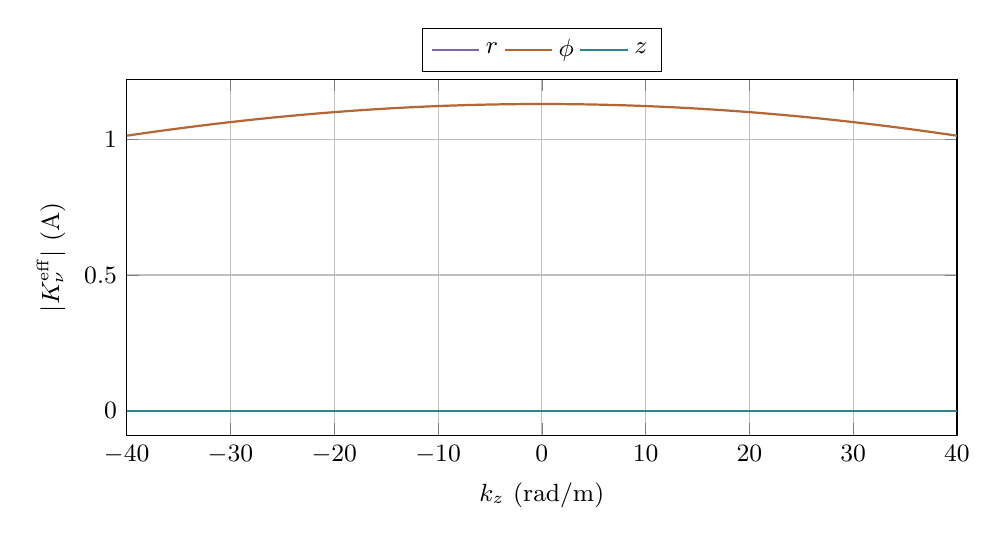
\begin{tikzpicture}
\begin{axis}[width=\linewidth,height=6.1cm,grid=major,
xlabel={$k_z$ (rad/m)},ylabel={$|K^{\rm eff}_\nu|$ (A)},
tick label style={font=\small},label style={font=\small},
legend style={font=\small,at={(.5,1.02)},anchor=south,legend columns=3},
xmin=-40,xmax=40,enlarge y limits=.08]
\addplot[violet,thick,no marks] coordinates {(-40,0) (-39,0) (-38,0) (-37,0) (-36,0) (-35,0) (-34,0) (-33,0) (-32,0) (-31,0) (-30,0) (-29,0) (-28,0) (-27,0) (-26,0) (-25,0) (-24,0) (-23,0) (-22,0) (-21,0) (-20,0) (-19,0) (-18,0) (-17,0) (-16,0) (-15,0) (-14,0) (-13,0) (-12,0) (-11,0) (-10,0) (-9,0) (-8,0) (-7,0) (-6,0) (-5,0) (-4,0) (-3,0) (-2,0) (-1,0) (0,0) (1,0) (2,0) (3,0) (4,0) (5,0) (6,0) (7,0) (8,0) (9,0) (10,0) (11,0) (12,0) (13,0) (14,0) (15,0) (16,0) (17,0) (18,0) (19,0) (20,0) (21,0) (22,0) (23,0) (24,0) (25,0) (26,0) (27,0) (28,0) (29,0) (30,0) (31,0) (32,0) (33,0) (34,0) (35,0) (36,0) (37,0) (38,0) (39,0) (40,0)};
\addlegendentry{$r$}
\addplot[copper,thick,no marks] coordinates {(-40,1.01344702359) (-39,1.01903606396) (-38,1.02450093716) (-37,1.02984034689) (-36,1.03505302579) (-35,1.04013773587) (-34,1.04509326881) (-33,1.04991844633) (-32,1.05461212052) (-31,1.05917317416) (-30,1.06360052107) (-29,1.06789310636) (-28,1.07204990676) (-27,1.07606993095) (-26,1.07995221978) (-25,1.08369584656) (-24,1.08729991735) (-23,1.09076357121) (-22,1.09408598039) (-21,1.09726635066) (-20,1.10030392144) (-19,1.10319796611) (-18,1.10594779211) (-17,1.10855274126) (-16,1.11101218984) (-15,1.11332554883) (-14,1.11549226405) (-13,1.11751181636) (-12,1.11938372174) (-11,1.12110753148) (-10,1.12268283229) (-9,1.12410924644) (-8,1.12538643182) (-7,1.1265140821) (-6,1.12749192675) (-5,1.12831973118) (-4,1.12899729676) (-3,1.12952446091) (-2,1.12990109712) (-1,1.13012711501) (0,1.13020246034) (1,1.13012711501) (2,1.12990109712) (3,1.12952446091) (4,1.12899729676) (5,1.12831973118) (6,1.12749192675) (7,1.1265140821) (8,1.12538643182) (9,1.12410924644) (10,1.12268283229) (11,1.12110753148) (12,1.11938372174) (13,1.11751181636) (14,1.11549226405) (15,1.11332554883) (16,1.11101218984) (17,1.10855274126) (18,1.10594779211) (19,1.10319796611) (20,1.10030392144) (21,1.09726635066) (22,1.09408598039) (23,1.09076357121) (24,1.08729991735) (25,1.08369584656) (26,1.07995221978) (27,1.07606993095) (28,1.07204990676) (29,1.06789310636) (30,1.06360052107) (31,1.05917317416) (32,1.05461212052) (33,1.04991844633) (34,1.04509326881) (35,1.04013773587) (36,1.03505302579) (37,1.02984034689) (38,1.02450093716) (39,1.01903606396) (40,1.01344702359)};
\addlegendentry{$\phi$}
\addplot[teal,thick,no marks] coordinates {(-40,0) (-39,0) (-38,0) (-37,0) (-36,0) (-35,0) (-34,0) (-33,0) (-32,0) (-31,0) (-30,0) (-29,0) (-28,0) (-27,0) (-26,0) (-25,0) (-24,0) (-23,0) (-22,0) (-21,0) (-20,0) (-19,0) (-18,0) (-17,0) (-16,0) (-15,0) (-14,0) (-13,0) (-12,0) (-11,0) (-10,0) (-9,0) (-8,0) (-7,0) (-6,0) (-5,0) (-4,0) (-3,0) (-2,0) (-1,0) (0,0) (1,0) (2,0) (3,0) (4,0) (5,0) (6,0) (7,0) (8,0) (9,0) (10,0) (11,0) (12,0) (13,0) (14,0) (15,0) (16,0) (17,0) (18,0) (19,0) (20,0) (21,0) (22,0) (23,0) (24,0) (25,0) (26,0) (27,0) (28,0) (29,0) (30,0) (31,0) (32,0) (33,0) (34,0) (35,0) (36,0) (37,0) (38,0) (39,0) (40,0)};
\addlegendentry{$z$}
\end{axis}\end{tikzpicture}}
\par\small 展示汇总谱，$m=1$；场加载保留各源半径。
\end{minipage}
% END GENERATED: prescribed_current_15
\end{center}

\subsection{鸟笼给定电流网络（编号 16）}
在 $r=b$ 上给定 $N\ge3$ 条轴向腿，
$\phi_j=j d_\phi$、$d_\phi=2\pi/N$，腿从 $-L/2$ 指向 $+L/2$。
指定腿电流为 $IG_j$，$G_j=\cos(q\phi_j)$ 或 $\ee^{\ii q\phi_j}$；
取整数 $1\le q<N$，保证 $\sum_jG_j=0$。
上、下端环弧均以 $+\phi$ 为参考方向，分别赋电流 $IT_j$、$-IT_j$，其中
\begin{equation}\label{eq:birdcageRing}
 \mathcal T_j=\frac{\ee^{\ii q\phi_j}}{1-\ee^{-\ii qd_\phi}},\qquad
 T_j=\begin{cases}\RePart\mathcal T_j,&G_j=\cos(q\phi_j),\\
 \mathcal T_j,&G_j=\ee^{\ii q\phi_j}.\end{cases}
\end{equation}
于是 $T_j-T_{j-1}=G_j$，每个节点的流入、流出电流相等。
选择 $\sum_jT_j=0$ 固定端环的额外均匀环流为零；这是给定电流约定。
\textbf{这些端环电流直接由所选分布规定，不是求解电容或谐振得到的。}
因此名称标为“鸟笼电流”，不输出该鸟笼的电路谐振频率。

记单弧积分
$H_m(\phi,d)=d\ee^{-\ii m(\phi+d/2)}\sinc(md/2)$。
轴向腿与端环分别给出
\begin{equation}\label{eq:birdcageSource}
 \begin{aligned}
 K_z&=\frac{CW_\phi L}{2\pi b}\sinc(k_zL/2)
 \sum_jG_j\ee^{-\ii m\phi_j},\\
 K_\phi&=\frac{CW_\phi}{2\pi}
 [\ee^{-\ii k_zL/2}-\ee^{\ii k_zL/2}]
 \sum_jT_jH_m(\phi_j,d_\phi),\qquad K_r=0.
 \end{aligned}
\end{equation}
旋转相位分布具有离散选择 $m\equiv q\pmod N$；余弦驻波含有正、负两个角向谐波及其离散混叠。
腿电流满足给定幅值不意味着所有端环也承载相同幅值。
\begin{center}% BEGIN GENERATED: prescribed_current_16
% Current geometry exported by C; arrows show instantaneous real current at t=0.
\begin{minipage}[t]{.48\linewidth}\centering\vspace{0pt}
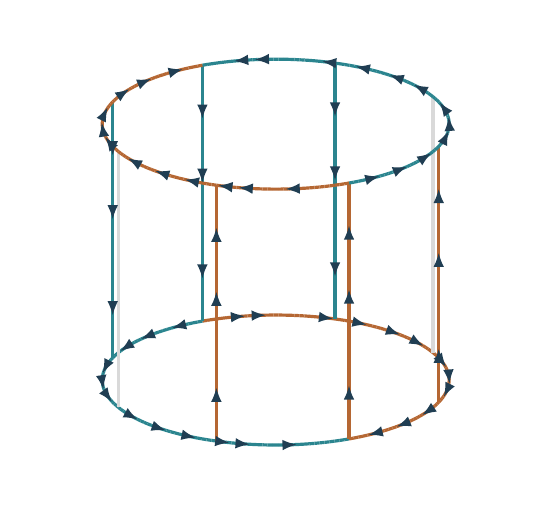
\begin{tikzpicture}[x=1cm,y=1cm,>=Latex,font=\small]
\path[use as bounding box] (-3.15,-2.85) rectangle (3.15,2.85);
\draw[copper,line width=1.15pt] (-0.02958,-0.79961)--(0.03697,-0.79965);
\draw[copper,line width=1.15pt] (-0.09609,-0.80032)--(-0.02958,-0.79961);
\draw[copper,line width=1.15pt] (0.03697,-0.79965)--(0.10348,-0.80045);
\draw[copper,line width=1.15pt] (-0.16253,-0.80179)--(-0.09609,-0.80032);
\draw[copper,line width=1.15pt] (0.10348,-0.80045)--(0.16990,-0.80199);
\draw[copper,line width=1.15pt] (-0.22881,-0.80400)--(-0.16253,-0.80179);
\draw[copper,line width=1.15pt] (0.16990,-0.80199)--(0.23616,-0.80429);
\draw[copper,line width=1.15pt] (-0.29488,-0.80696)--(-0.22881,-0.80400);
\draw[copper,line width=1.15pt] (0.23616,-0.80429)--(0.30221,-0.80734);
\draw[copper,line width=1.15pt] (-0.36069,-0.81067)--(-0.29488,-0.80696);
\draw[copper,line width=1.15pt] (0.30221,-0.80734)--(0.36798,-0.81113);
\draw[copper,line width=1.15pt] (-0.42616,-0.81512)--(-0.36069,-0.81067);
\draw[copper,line width=1.15pt] (0.36798,-0.81113)--(0.43342,-0.81567);
\draw[copper,line width=1.15pt] (-0.49125,-0.82032)--(-0.42616,-0.81512);
\draw[copper,line width=1.15pt] (0.43342,-0.81567)--(0.49846,-0.82094);
\draw[copper,line width=1.15pt] (-0.55589,-0.82624)--(-0.49125,-0.82032);
\draw[copper,line width=1.15pt] (0.49846,-0.82094)--(0.56304,-0.82694);
\draw[copper,line width=1.15pt] (-0.62002,-0.83289)--(-0.55589,-0.82624);
\draw[copper,line width=1.15pt] (0.56304,-0.82694)--(0.62711,-0.83368);
\draw[copper,line width=1.15pt] (-0.68359,-0.84027)--(-0.62002,-0.83289);
\draw[copper,line width=1.15pt] (0.62711,-0.83368)--(0.69061,-0.84113);
\draw[copper,line width=1.15pt] (-0.74653,-0.84836)--(-0.68359,-0.84027);
\draw[copper,line width=1.15pt] (0.69061,-0.84113)--(0.75348,-0.84931);
\draw[copper,line width=1.15pt] (-0.80879,-0.85716)--(-0.74653,-0.84836);
\draw[copper,line width=1.15pt] (0.75348,-0.84931)--(0.81566,-0.85819);
\draw[copper,line width=1.15pt] (-0.87031,-0.86666)--(-0.80879,-0.85716);
\draw[copper,line width=1.15pt] (0.81566,-0.85819)--(0.87710,-0.86776);
\draw[copper,line width=1.15pt] (-0.93104,-0.87686)--(-0.87031,-0.86666);
\draw[copper,line width=1.15pt] (0.87710,-0.86776)--(0.93774,-0.87803);
\draw[teal,line width=1.15pt] (-0.99092,-0.88773)--(-0.93104,-0.87686);
\draw[teal,line width=1.15pt] (0.75348,-0.84931)--(0.75348,-0.44310);
\draw[copper,line width=1.15pt] (0.93774,-0.87803)--(0.99752,-0.88898);
\draw[teal,line width=1.15pt] (-1.04989,-0.89928)--(-0.99092,-0.88773);
\draw[copper,line width=1.15pt] (0.99752,-0.88898)--(1.05639,-0.90060);
\draw[teal,line width=1.15pt] (-1.10791,-0.91149)--(-1.04989,-0.89928);
\draw[copper,line width=1.15pt] (1.05639,-0.90060)--(1.11430,-0.91289);
\draw[teal,line width=1.15pt] (-0.93104,-0.87686)--(-0.93104,-0.47066);
\draw[teal,line width=1.15pt] (-1.16492,-0.92435)--(-1.10791,-0.91149);
\draw[copper,line width=1.15pt] (1.11430,-0.91289)--(1.17119,-0.92582);
\draw[teal,line width=1.15pt] (-1.22086,-0.93785)--(-1.16492,-0.92435);
\draw[copper,line width=1.15pt] (1.17119,-0.92582)--(1.22701,-0.93939);
\draw[teal,line width=1.15pt] (-1.27569,-0.95198)--(-1.22086,-0.93785);
\draw[copper,line width=1.15pt] (1.22701,-0.93939)--(1.28171,-0.95359);
\draw[teal,line width=1.15pt] (0.75348,-0.44310)--(0.75348,-0.03690);
\draw[teal,line width=1.15pt] (-1.32936,-0.96672)--(-1.27569,-0.95198);
\draw[copper,line width=1.15pt] (1.28171,-0.95359)--(1.33524,-0.96839);
\draw[teal,line width=1.15pt] (-1.38181,-0.98206)--(-1.32936,-0.96672);
\draw[copper,line width=1.15pt] (1.33524,-0.96839)--(1.38756,-0.98380);
\draw[teal,line width=1.15pt] (-0.93104,-0.47066)--(-0.93104,-0.06445);
\draw[teal,line width=1.15pt] (-1.43300,-0.99799)--(-1.38181,-0.98206);
\draw[copper,line width=1.15pt] (1.38756,-0.98380)--(1.43861,-0.99979);
\draw[teal,line width=1.15pt] (-1.48288,-1.01449)--(-1.43300,-0.99799);
\draw[copper,line width=1.15pt] (1.43861,-0.99979)--(1.48834,-1.01635);
\draw[teal,line width=1.15pt] (0.75348,-0.03690)--(0.75348,0.36930);
\draw[teal,line width=1.15pt] (-1.53142,-1.03154)--(-1.48288,-1.01449);
\draw[copper,line width=1.15pt] (1.48834,-1.01635)--(1.53672,-1.03347);
\draw[teal,line width=1.15pt] (-1.57855,-1.04914)--(-1.53142,-1.03154);
\draw[copper,line width=1.15pt] (1.53672,-1.03347)--(1.58370,-1.05113);
\draw[teal,line width=1.15pt] (-0.93104,-0.06445)--(-0.93104,0.34175);
\draw[teal,line width=1.15pt] (-1.62424,-1.06726)--(-1.57855,-1.04914);
\draw[copper,line width=1.15pt] (1.58370,-1.05113)--(1.62923,-1.06931);
\draw[teal,line width=1.15pt] (-1.66845,-1.08589)--(-1.62424,-1.06726);
\draw[copper,line width=1.15pt] (1.62923,-1.06931)--(1.67327,-1.08799);
\draw[teal,line width=1.15pt] (0.75348,0.36930)--(0.75348,0.77550);
\draw[teal,line width=1.15pt] (-1.71114,-1.10502)--(-1.66845,-1.08589);
\draw[copper,line width=1.15pt] (1.67327,-1.08799)--(1.71579,-1.10717);
\draw[teal,line width=1.15pt] (-0.93104,0.34175)--(-0.93104,0.74795);
\draw[teal,line width=1.15pt] (-1.75227,-1.12461)--(-1.71114,-1.10502);
\draw[copper,line width=1.15pt] (1.71579,-1.10717)--(1.75674,-1.12682);
\draw[teal,line width=1.15pt] (-1.79180,-1.14467)--(-1.75227,-1.12461);
\draw[copper,line width=1.15pt] (1.75674,-1.12682)--(1.79609,-1.14692);
\draw[teal,line width=1.15pt] (0.75348,0.77550)--(0.75348,1.18170);
\draw[teal,line width=1.15pt] (-1.82969,-1.16516)--(-1.79180,-1.14467);
\draw[copper,line width=1.15pt] (1.79609,-1.14692)--(1.83380,-1.16746);
\draw[teal,line width=1.15pt] (-0.93104,0.74795)--(-0.93104,1.15415);
\draw[teal,line width=1.15pt] (-1.86592,-1.18607)--(-1.82969,-1.16516);
\draw[copper,line width=1.15pt] (1.83380,-1.16746)--(1.86984,-1.18842);
\draw[teal,line width=1.15pt] (-1.90044,-1.20738)--(-1.86592,-1.18607);
\draw[copper,line width=1.15pt] (1.86984,-1.18842)--(1.90417,-1.20977);
\draw[teal,line width=1.15pt] (0.75348,1.18170)--(0.75348,1.58790);
\draw[teal,line width=1.15pt] (-1.93323,-1.22908)--(-1.90044,-1.20738);
\draw[copper,line width=1.15pt] (1.90417,-1.20977)--(1.93676,-1.23151);
\draw[teal,line width=1.15pt] (-1.96425,-1.25113)--(-1.93323,-1.22908);
\draw[teal,line width=1.15pt] (-0.93104,1.15415)--(-0.93104,1.56035);
\draw[copper,line width=1.15pt] (1.93676,-1.23151)--(1.96759,-1.25360);
\draw[teal,line width=1.15pt] (-1.99349,-1.27352)--(-1.96425,-1.25113);
\draw[copper,line width=1.15pt] (1.96759,-1.25360)--(1.99662,-1.27603);
\draw[teal,line width=1.15pt] (0.75348,1.58790)--(0.75348,1.99410);
\draw[teal,line width=1.15pt] (-2.02090,-1.29624)--(-1.99349,-1.27352);
\draw[copper,line width=1.15pt] (1.99662,-1.27603)--(2.02383,-1.29878);
\draw[teal,line width=1.15pt] (-2.04647,-1.31925)--(-2.02090,-1.29624);
\draw[teal,line width=1.15pt] (-0.93104,1.56035)--(-0.93104,1.96655);
\draw[gray!30,line width=1.15pt] (1.99662,-1.27603)--(1.99662,-0.86983);
\draw[copper,line width=1.15pt] (2.02383,-1.29878)--(2.04919,-1.32183);
\draw[teal,line width=1.15pt] (-0.02958,2.45000)--(0.03697,2.44996);
\draw[teal,line width=1.15pt] (-0.09609,2.44929)--(-0.02958,2.45000);
\draw[teal,line width=1.15pt] (0.03697,2.44996)--(0.10348,2.44916);
\draw[teal,line width=1.15pt] (-2.07017,-1.34255)--(-2.04647,-1.31925);
\draw[teal,line width=1.15pt] (-0.16253,2.44783)--(-0.09609,2.44929);
\draw[teal,line width=1.15pt] (0.10348,2.44916)--(0.16990,2.44762);
\draw[teal,line width=1.15pt] (-0.22881,2.44561)--(-0.16253,2.44783);
\draw[copper,line width=1.15pt] (2.04919,-1.32183)--(2.07269,-1.34515);
\draw[teal,line width=1.15pt] (0.16990,2.44762)--(0.23616,2.44532);
\draw[teal,line width=1.15pt] (-0.29488,2.44265)--(-0.22881,2.44561);
\draw[teal,line width=1.15pt] (0.23616,2.44532)--(0.30221,2.44227);
\draw[teal,line width=1.15pt] (-0.36069,2.43894)--(-0.29488,2.44265);
\draw[teal,line width=1.15pt] (0.30221,2.44227)--(0.36798,2.43848);
\draw[teal,line width=1.15pt] (-0.42616,2.43449)--(-0.36069,2.43894);
\draw[teal,line width=1.15pt] (0.36798,2.43848)--(0.43342,2.43395);
\draw[teal,line width=1.15pt] (0.75348,1.99410)--(0.75348,2.40030);
\draw[teal,line width=1.15pt] (-0.49125,2.42930)--(-0.42616,2.43449);
\draw[teal,line width=1.15pt] (0.43342,2.43395)--(0.49846,2.42867);
\draw[teal,line width=1.15pt] (-0.55589,2.42337)--(-0.49125,2.42930);
\draw[teal,line width=1.15pt] (-2.09198,-1.36610)--(-2.07017,-1.34255);
\draw[teal,line width=1.15pt] (0.49846,2.42867)--(0.56304,2.42267);
\draw[copper,line width=1.15pt] (2.07269,-1.34515)--(2.09429,-1.36873);
\draw[teal,line width=1.15pt] (-0.62002,2.41672)--(-0.55589,2.42337);
\draw[teal,line width=1.15pt] (0.56304,2.42267)--(0.62711,2.41593);
\draw[teal,line width=1.15pt] (-0.68359,2.40934)--(-0.62002,2.41672);
\draw[teal,line width=1.15pt] (0.62711,2.41593)--(0.69061,2.40848);
\draw[teal,line width=1.15pt] (-0.93104,1.96655)--(-0.93104,2.37275);
\draw[teal,line width=1.15pt] (-0.74653,2.40125)--(-0.68359,2.40934);
\draw[gray!30,line width=1.15pt] (1.99662,-0.86983)--(1.99662,-0.46363);
\draw[teal,line width=1.15pt] (0.69061,2.40848)--(0.75348,2.40030);
\draw[teal,line width=1.15pt] (-2.07017,-1.34255)--(-2.07017,-0.93635);
\draw[teal,line width=1.15pt] (-2.11189,-1.38989)--(-2.09198,-1.36610);
\draw[copper,line width=1.15pt] (2.09429,-1.36873)--(2.11398,-1.39254);
\draw[teal,line width=1.15pt] (-0.80879,2.39245)--(-0.74653,2.40125);
\draw[teal,line width=1.15pt] (0.75348,2.40030)--(0.81566,2.39143);
\draw[teal,line width=1.15pt] (-0.87031,2.38295)--(-0.80879,2.39245);
\draw[teal,line width=1.15pt] (0.81566,2.39143)--(0.87710,2.38185);
\draw[teal,line width=1.15pt] (-2.12986,-1.41389)--(-2.11189,-1.38989);
\draw[teal,line width=1.15pt] (-0.93104,2.37275)--(-0.87031,2.38295);
\draw[teal,line width=1.15pt] (0.87710,2.38185)--(0.93774,2.37158);
\draw[copper,line width=1.15pt] (2.11398,-1.39254)--(2.13174,-1.41657);
\draw[copper,line width=1.15pt] (-0.99092,2.36188)--(-0.93104,2.37275);
\draw[teal,line width=1.15pt] (0.93774,2.37158)--(0.99752,2.36063);
\draw[copper,line width=1.15pt] (-1.04989,2.35033)--(-0.99092,2.36188);
\draw[teal,line width=1.15pt] (0.99752,2.36063)--(1.05639,2.34901);
\draw[teal,line width=1.15pt] (-2.14590,-1.43808)--(-2.12986,-1.41389);
\draw[copper,line width=1.15pt] (2.13174,-1.41657)--(2.14756,-1.44078);
\draw[copper,line width=1.15pt] (-1.10791,2.33812)--(-1.04989,2.35033);
\draw[teal,line width=1.15pt] (1.05639,2.34901)--(1.11430,2.33672);
\draw[gray!30,line width=1.15pt] (1.99662,-0.46363)--(1.99662,-0.05743);
\draw[teal,line width=1.15pt] (-2.07017,-0.93635)--(-2.07017,-0.53014);
\draw[copper,line width=1.15pt] (-1.16492,2.32526)--(-1.10791,2.33812);
\draw[teal,line width=1.15pt] (1.11430,2.33672)--(1.17119,2.32379);
\draw[teal,line width=1.15pt] (-2.15997,-1.46245)--(-2.14590,-1.43808);
\draw[copper,line width=1.15pt] (2.14756,-1.44078)--(2.16142,-1.46516);
\draw[copper,line width=1.15pt] (-1.22086,2.31176)--(-1.16492,2.32526);
\draw[teal,line width=1.15pt] (1.17119,2.32379)--(1.22701,2.31022);
\draw[teal,line width=1.15pt] (-2.17208,-1.48696)--(-2.15997,-1.46245);
\draw[copper,line width=1.15pt] (-1.27569,2.29763)--(-1.22086,2.31176);
\draw[teal,line width=1.15pt] (1.22701,2.31022)--(1.28171,2.29603);
\draw[copper,line width=1.15pt] (2.16142,-1.46516)--(2.17330,-1.48969);
\draw[copper,line width=1.15pt] (-1.32936,2.28289)--(-1.27569,2.29763);
\draw[teal,line width=1.15pt] (1.28171,2.29603)--(1.33524,2.28122);
\draw[teal,line width=1.15pt] (-2.18220,-1.51160)--(-2.17208,-1.48696);
\draw[copper,line width=1.15pt] (2.17330,-1.48969)--(2.18320,-1.51434);
\draw[copper,line width=1.15pt] (-1.38181,2.26755)--(-1.32936,2.28289);
\draw[teal,line width=1.15pt] (1.33524,2.28122)--(1.38756,2.26581);
\draw[gray!30,line width=1.15pt] (1.99662,-0.05743)--(1.99662,0.34877);
\draw[teal,line width=1.15pt] (-2.07017,-0.53014)--(-2.07017,-0.12394);
\draw[copper,line width=1.15pt] (-1.43300,2.25162)--(-1.38181,2.26755);
\draw[teal,line width=1.15pt] (1.38756,2.26581)--(1.43861,2.24982);
\draw[teal,line width=1.15pt] (-2.19033,-1.53634)--(-2.18220,-1.51160);
\draw[copper,line width=1.15pt] (2.18320,-1.51434)--(2.19111,-1.53909);
\draw[copper,line width=1.15pt] (-1.48288,2.23513)--(-1.43300,2.25162);
\draw[teal,line width=1.15pt] (1.43861,2.24982)--(1.48834,2.23326);
\draw[teal,line width=1.15pt] (-2.19647,-1.56116)--(-2.19033,-1.53634);
\draw[copper,line width=1.15pt] (2.19111,-1.53909)--(2.19703,-1.56392);
\draw[copper,line width=1.15pt] (-1.53142,2.21807)--(-1.48288,2.23513);
\draw[teal,line width=1.15pt] (1.48834,2.23326)--(1.53672,2.21614);
\draw[copper,line width=1.15pt] (-1.57855,2.20047)--(-1.53142,2.21807);
\draw[teal,line width=1.15pt] (1.53672,2.21614)--(1.58370,2.19848);
\draw[teal,line width=1.15pt] (-2.20060,-1.58604)--(-2.19647,-1.56116);
\draw[gray!30,line width=1.15pt] (1.99662,0.34877)--(1.99662,0.75498);
\draw[teal,line width=1.15pt] (-2.07017,-0.12394)--(-2.07017,0.28226);
\draw[copper,line width=1.15pt] (2.19703,-1.56392)--(2.20093,-1.58881);
\draw[copper,line width=1.15pt] (-1.62424,2.18235)--(-1.57855,2.20047);
\draw[teal,line width=1.15pt] (1.58370,2.19848)--(1.62923,2.18030);
\draw[teal,line width=1.15pt] (-2.20272,-1.61096)--(-2.20060,-1.58604);
\draw[copper,line width=1.15pt] (2.20093,-1.58881)--(2.20283,-1.61373);
\draw[copper,line width=1.15pt] (-1.66845,2.16372)--(-1.62424,2.18235);
\draw[teal,line width=1.15pt] (1.62923,2.18030)--(1.67327,2.16162);
\draw[teal,line width=1.15pt] (-2.20283,-1.63588)--(-2.20272,-1.61096);
\draw[copper,line width=1.15pt] (-1.71114,2.14459)--(-1.66845,2.16372);
\draw[copper,line width=1.15pt] (2.20283,-1.61373)--(2.20272,-1.63865);
\draw[teal,line width=1.15pt] (1.67327,2.16162)--(1.71579,2.14244);
\draw[gray!30,line width=1.15pt] (1.99662,0.75498)--(1.99662,1.16118);
\draw[teal,line width=1.15pt] (-2.07017,0.28226)--(-2.07017,0.68846);
\draw[copper,line width=1.15pt] (-1.75227,2.12500)--(-1.71114,2.14459);
\draw[teal,line width=1.15pt] (1.71579,2.14244)--(1.75674,2.12279);
\draw[teal,line width=1.15pt] (-2.20093,-1.66080)--(-2.20283,-1.63588);
\draw[copper,line width=1.15pt] (2.20272,-1.63865)--(2.20060,-1.66357);
\draw[copper,line width=1.15pt] (-1.79180,2.10494)--(-1.75227,2.12500);
\draw[teal,line width=1.15pt] (1.75674,2.12279)--(1.79609,2.10269);
\draw[teal,line width=1.15pt] (-2.19703,-1.68569)--(-2.20093,-1.66080);
\draw[copper,line width=1.15pt] (2.20060,-1.66357)--(2.19647,-1.68845);
\draw[copper,line width=1.15pt] (-1.82969,2.08445)--(-1.79180,2.10494);
\draw[teal,line width=1.15pt] (1.79609,2.10269)--(1.83380,2.08215);
\draw[teal,line width=1.15pt] (-2.19111,-1.71052)--(-2.19703,-1.68569);
\draw[copper,line width=1.15pt] (2.19647,-1.68845)--(2.19033,-1.71327);
\draw[copper,line width=1.15pt] (-1.86592,2.06354)--(-1.82969,2.08445);
\draw[gray!30,line width=1.15pt] (1.99662,1.16118)--(1.99662,1.56738);
\draw[teal,line width=1.15pt] (-2.07017,0.68846)--(-2.07017,1.09466);
\draw[teal,line width=1.15pt] (1.83380,2.08215)--(1.86984,2.06119);
\draw[teal,line width=1.15pt] (-2.18320,-1.73527)--(-2.19111,-1.71052);
\draw[copper,line width=1.15pt] (2.19033,-1.71327)--(2.18220,-1.73801);
\draw[copper,line width=1.15pt] (-1.90044,2.04223)--(-1.86592,2.06354);
\draw[teal,line width=1.15pt] (1.86984,2.06119)--(1.90417,2.03984);
\draw[teal,line width=1.15pt] (-2.17330,-1.75992)--(-2.18320,-1.73527);
\draw[copper,line width=1.15pt] (-1.93323,2.02054)--(-1.90044,2.04223);
\draw[copper,line width=1.15pt] (2.18220,-1.73801)--(2.17208,-1.76265);
\draw[teal,line width=1.15pt] (1.90417,2.03984)--(1.93676,2.01810);
\draw[copper,line width=1.15pt] (-1.96425,1.99848)--(-1.93323,2.02054);
\draw[teal,line width=1.15pt] (-2.16142,-1.78445)--(-2.17330,-1.75992);
\draw[teal,line width=1.15pt] (1.93676,2.01810)--(1.96759,1.99601);
\draw[gray!30,line width=1.15pt] (1.99662,1.56738)--(1.99662,1.97358);
\draw[teal,line width=1.15pt] (-2.07017,1.09466)--(-2.07017,1.50086);
\draw[copper,line width=1.15pt] (2.17208,-1.76265)--(2.15997,-1.78717);
\draw[copper,line width=1.15pt] (-1.99349,1.97609)--(-1.96425,1.99848);
\draw[teal,line width=1.15pt] (1.96759,1.99601)--(1.99662,1.97358);
\draw[teal,line width=1.15pt] (-2.14756,-1.80883)--(-2.16142,-1.78445);
\draw[copper,line width=1.15pt] (2.15997,-1.78717)--(2.14590,-1.81153);
\draw[copper,line width=1.15pt] (-2.02090,1.95337)--(-1.99349,1.97609);
\draw[teal,line width=1.15pt] (1.99662,1.97358)--(2.02383,1.95083);
\draw[teal,line width=1.15pt] (-2.13174,-1.83304)--(-2.14756,-1.80883);
\draw[copper,line width=1.15pt] (2.14590,-1.81153)--(2.12986,-1.83572);
\draw[copper,line width=1.15pt] (-2.04647,1.93036)--(-2.02090,1.95337);
\draw[teal,line width=1.15pt] (-2.07017,1.50086)--(-2.07017,1.90706);
\draw[teal,line width=1.15pt] (2.02383,1.95083)--(2.04919,1.92778);
\draw[teal,line width=1.15pt] (-2.11398,-1.85707)--(-2.13174,-1.83304);
\draw[copper,line width=1.15pt] (2.12986,-1.83572)--(2.11189,-1.85973);
\draw[copper,line width=1.15pt] (-2.07017,1.90706)--(-2.04647,1.93036);
\draw[teal,line width=1.15pt] (2.04919,1.92778)--(2.07269,1.90446);
\draw[teal,line width=1.15pt] (-2.09429,-1.88088)--(-2.11398,-1.85707);
\draw[copper,line width=1.15pt] (2.11189,-1.85973)--(2.09198,-1.88351);
\draw[copper,line width=1.15pt] (-2.09198,1.88351)--(-2.07017,1.90706);
\draw[teal,line width=1.15pt] (2.07269,1.90446)--(2.09429,1.88088);
\draw[teal,line width=1.15pt] (-2.07269,-1.90446)--(-2.09429,-1.88088);
\draw[copper,line width=1.15pt] (2.09198,-1.88351)--(2.07017,-1.90706);
\draw[copper,line width=1.15pt] (-2.11189,1.85973)--(-2.09198,1.88351);
\draw[teal,line width=1.15pt] (2.09429,1.88088)--(2.11398,1.85707);
\draw[teal,line width=1.15pt] (-2.04919,-1.92778)--(-2.07269,-1.90446);
\draw[copper,line width=1.15pt] (2.07017,-1.90706)--(2.04647,-1.93036);
\draw[copper,line width=1.15pt] (-2.12986,1.83572)--(-2.11189,1.85973);
\draw[teal,line width=1.15pt] (2.11398,1.85707)--(2.13174,1.83304);
\draw[teal,line width=1.15pt] (-2.02383,-1.95083)--(-2.04919,-1.92778);
\draw[copper,line width=1.15pt] (2.07017,-1.90706)--(2.07017,-1.50086);
\draw[copper,line width=1.15pt] (2.04647,-1.93036)--(2.02090,-1.95337);
\draw[copper,line width=1.15pt] (-2.14590,1.81153)--(-2.12986,1.83572);
\draw[teal,line width=1.15pt] (2.13174,1.83304)--(2.14756,1.80883);
\draw[teal,line width=1.15pt] (-1.99662,-1.97358)--(-2.02383,-1.95083);
\draw[copper,line width=1.15pt] (2.02090,-1.95337)--(1.99349,-1.97609);
\draw[copper,line width=1.15pt] (-2.15997,1.78717)--(-2.14590,1.81153);
\draw[teal,line width=1.15pt] (2.14756,1.80883)--(2.16142,1.78445);
\draw[teal,line width=1.15pt] (-1.96759,-1.99601)--(-1.99662,-1.97358);
\draw[copper,line width=1.15pt] (1.99349,-1.97609)--(1.96425,-1.99848);
\draw[copper,line width=1.15pt] (-2.17208,1.76265)--(-2.15997,1.78717);
\draw[copper,line width=1.15pt] (2.07017,-1.50086)--(2.07017,-1.09466);
\draw[gray!30,line width=1.15pt] (-1.99662,-1.97358)--(-1.99662,-1.56738);
\draw[teal,line width=1.15pt] (-1.93676,-2.01810)--(-1.96759,-1.99601);
\draw[teal,line width=1.15pt] (2.16142,1.78445)--(2.17330,1.75992);
\draw[copper,line width=1.15pt] (1.96425,-1.99848)--(1.93323,-2.02054);
\draw[teal,line width=1.15pt] (-1.90417,-2.03984)--(-1.93676,-2.01810);
\draw[copper,line width=1.15pt] (-2.18220,1.73801)--(-2.17208,1.76265);
\draw[copper,line width=1.15pt] (1.93323,-2.02054)--(1.90044,-2.04223);
\draw[teal,line width=1.15pt] (2.17330,1.75992)--(2.18320,1.73527);
\draw[teal,line width=1.15pt] (-1.86984,-2.06119)--(-1.90417,-2.03984);
\draw[copper,line width=1.15pt] (1.90044,-2.04223)--(1.86592,-2.06354);
\draw[copper,line width=1.15pt] (-2.19033,1.71327)--(-2.18220,1.73801);
\draw[teal,line width=1.15pt] (2.18320,1.73527)--(2.19111,1.71052);
\draw[teal,line width=1.15pt] (-1.83380,-2.08215)--(-1.86984,-2.06119);
\draw[copper,line width=1.15pt] (2.07017,-1.09466)--(2.07017,-0.68846);
\draw[gray!30,line width=1.15pt] (-1.99662,-1.56738)--(-1.99662,-1.16118);
\draw[copper,line width=1.15pt] (1.86592,-2.06354)--(1.82969,-2.08445);
\draw[copper,line width=1.15pt] (-2.19647,1.68845)--(-2.19033,1.71327);
\draw[teal,line width=1.15pt] (2.19111,1.71052)--(2.19703,1.68569);
\draw[teal,line width=1.15pt] (-1.79609,-2.10269)--(-1.83380,-2.08215);
\draw[copper,line width=1.15pt] (1.82969,-2.08445)--(1.79180,-2.10494);
\draw[copper,line width=1.15pt] (-2.20060,1.66357)--(-2.19647,1.68845);
\draw[teal,line width=1.15pt] (2.19703,1.68569)--(2.20093,1.66080);
\draw[teal,line width=1.15pt] (-1.75674,-2.12279)--(-1.79609,-2.10269);
\draw[copper,line width=1.15pt] (1.79180,-2.10494)--(1.75227,-2.12500);
\draw[copper,line width=1.15pt] (-2.20272,1.63865)--(-2.20060,1.66357);
\draw[teal,line width=1.15pt] (2.20093,1.66080)--(2.20283,1.63588);
\draw[teal,line width=1.15pt] (-1.71579,-2.14244)--(-1.75674,-2.12279);
\draw[copper,line width=1.15pt] (1.75227,-2.12500)--(1.71114,-2.14459);
\draw[copper,line width=1.15pt] (2.07017,-0.68846)--(2.07017,-0.28226);
\draw[gray!30,line width=1.15pt] (-1.99662,-1.16118)--(-1.99662,-0.75498);
\draw[teal,line width=1.15pt] (-1.67327,-2.16162)--(-1.71579,-2.14244);
\draw[copper,line width=1.15pt] (-2.20283,1.61373)--(-2.20272,1.63865);
\draw[copper,line width=1.15pt] (1.71114,-2.14459)--(1.66845,-2.16372);
\draw[teal,line width=1.15pt] (2.20283,1.63588)--(2.20272,1.61096);
\draw[teal,line width=1.15pt] (-1.62923,-2.18030)--(-1.67327,-2.16162);
\draw[copper,line width=1.15pt] (1.66845,-2.16372)--(1.62424,-2.18235);
\draw[copper,line width=1.15pt] (-2.20093,1.58881)--(-2.20283,1.61373);
\draw[teal,line width=1.15pt] (2.20272,1.61096)--(2.20060,1.58604);
\draw[teal,line width=1.15pt] (-1.58370,-2.19848)--(-1.62923,-2.18030);
\draw[copper,line width=1.15pt] (1.62424,-2.18235)--(1.57855,-2.20047);
\draw[copper,line width=1.15pt] (-2.19703,1.56392)--(-2.20093,1.58881);
\draw[copper,line width=1.15pt] (2.07017,-0.28226)--(2.07017,0.12394);
\draw[gray!30,line width=1.15pt] (-1.99662,-0.75498)--(-1.99662,-0.34877);
\draw[teal,line width=1.15pt] (2.20060,1.58604)--(2.19647,1.56116);
\draw[teal,line width=1.15pt] (-1.53672,-2.21614)--(-1.58370,-2.19848);
\draw[copper,line width=1.15pt] (1.57855,-2.20047)--(1.53142,-2.21807);
\draw[teal,line width=1.15pt] (-1.48834,-2.23326)--(-1.53672,-2.21614);
\draw[copper,line width=1.15pt] (1.53142,-2.21807)--(1.48288,-2.23513);
\draw[copper,line width=1.15pt] (-2.19111,1.53909)--(-2.19703,1.56392);
\draw[teal,line width=1.15pt] (2.19647,1.56116)--(2.19033,1.53634);
\draw[teal,line width=1.15pt] (-1.43861,-2.24982)--(-1.48834,-2.23326);
\draw[copper,line width=1.15pt] (1.48288,-2.23513)--(1.43300,-2.25162);
\draw[copper,line width=1.15pt] (-2.18320,1.51434)--(-2.19111,1.53909);
\draw[teal,line width=1.15pt] (2.19033,1.53634)--(2.18220,1.51160);
\draw[teal,line width=1.15pt] (-1.38756,-2.26581)--(-1.43861,-2.24982);
\draw[copper,line width=1.15pt] (1.43300,-2.25162)--(1.38181,-2.26755);
\draw[copper,line width=1.15pt] (2.07017,0.12394)--(2.07017,0.53014);
\draw[gray!30,line width=1.15pt] (-1.99662,-0.34877)--(-1.99662,0.05743);
\draw[teal,line width=1.15pt] (-1.33524,-2.28122)--(-1.38756,-2.26581);
\draw[copper,line width=1.15pt] (1.38181,-2.26755)--(1.32936,-2.28289);
\draw[copper,line width=1.15pt] (-2.17330,1.48969)--(-2.18320,1.51434);
\draw[teal,line width=1.15pt] (2.18220,1.51160)--(2.17208,1.48696);
\draw[teal,line width=1.15pt] (-1.28171,-2.29603)--(-1.33524,-2.28122);
\draw[copper,line width=1.15pt] (1.32936,-2.28289)--(1.27569,-2.29763);
\draw[copper,line width=1.15pt] (-2.16142,1.46516)--(-2.17330,1.48969);
\draw[teal,line width=1.15pt] (-1.22701,-2.31022)--(-1.28171,-2.29603);
\draw[copper,line width=1.15pt] (1.27569,-2.29763)--(1.22086,-2.31176);
\draw[teal,line width=1.15pt] (2.17208,1.48696)--(2.15997,1.46245);
\draw[teal,line width=1.15pt] (-1.17119,-2.32379)--(-1.22701,-2.31022);
\draw[copper,line width=1.15pt] (1.22086,-2.31176)--(1.16492,-2.32526);
\draw[copper,line width=1.15pt] (-2.14756,1.44078)--(-2.16142,1.46516);
\draw[teal,line width=1.15pt] (2.15997,1.46245)--(2.14590,1.43808);
\draw[teal,line width=1.15pt] (-1.11430,-2.33672)--(-1.17119,-2.32379);
\draw[copper,line width=1.15pt] (1.16492,-2.32526)--(1.10791,-2.33812);
\draw[copper,line width=1.15pt] (2.07017,0.53014)--(2.07017,0.93635);
\draw[gray!30,line width=1.15pt] (-1.99662,0.05743)--(-1.99662,0.46363);
\draw[teal,line width=1.15pt] (-1.05639,-2.34901)--(-1.11430,-2.33672);
\draw[copper,line width=1.15pt] (1.10791,-2.33812)--(1.04989,-2.35033);
\draw[copper,line width=1.15pt] (-2.13174,1.41657)--(-2.14756,1.44078);
\draw[teal,line width=1.15pt] (2.14590,1.43808)--(2.12986,1.41389);
\draw[teal,line width=1.15pt] (-0.99752,-2.36063)--(-1.05639,-2.34901);
\draw[copper,line width=1.15pt] (1.04989,-2.35033)--(0.99092,-2.36188);
\draw[teal,line width=1.15pt] (-0.93774,-2.37158)--(-0.99752,-2.36063);
\draw[copper,line width=1.15pt] (0.99092,-2.36188)--(0.93104,-2.37275);
\draw[copper,line width=1.15pt] (-2.11398,1.39254)--(-2.13174,1.41657);
\draw[teal,line width=1.15pt] (-0.87710,-2.38185)--(-0.93774,-2.37158);
\draw[teal,line width=1.15pt] (0.93104,-2.37275)--(0.87031,-2.38295);
\draw[teal,line width=1.15pt] (2.12986,1.41389)--(2.11189,1.38989);
\draw[teal,line width=1.15pt] (-0.81566,-2.39143)--(-0.87710,-2.38185);
\draw[teal,line width=1.15pt] (0.87031,-2.38295)--(0.80879,-2.39245);
\draw[teal,line width=1.15pt] (-0.75348,-2.40030)--(-0.81566,-2.39143);
\draw[teal,line width=1.15pt] (0.80879,-2.39245)--(0.74653,-2.40125);
\draw[copper,line width=1.15pt] (-2.09429,1.36873)--(-2.11398,1.39254);
\draw[teal,line width=1.15pt] (2.11189,1.38989)--(2.09198,1.36610);
\draw[copper,line width=1.15pt] (2.07017,0.93635)--(2.07017,1.34255);
\draw[teal,line width=1.15pt] (-0.69061,-2.40848)--(-0.75348,-2.40030);
\draw[gray!30,line width=1.15pt] (-1.99662,0.46363)--(-1.99662,0.86983);
\draw[teal,line width=1.15pt] (0.74653,-2.40125)--(0.68359,-2.40934);
\draw[copper,line width=1.15pt] (0.93104,-2.37275)--(0.93104,-1.96655);
\draw[teal,line width=1.15pt] (-0.62711,-2.41593)--(-0.69061,-2.40848);
\draw[teal,line width=1.15pt] (0.68359,-2.40934)--(0.62002,-2.41672);
\draw[teal,line width=1.15pt] (-0.56304,-2.42267)--(-0.62711,-2.41593);
\draw[teal,line width=1.15pt] (0.62002,-2.41672)--(0.55589,-2.42337);
\draw[copper,line width=1.15pt] (-2.07269,1.34515)--(-2.09429,1.36873);
\draw[teal,line width=1.15pt] (-0.49846,-2.42867)--(-0.56304,-2.42267);
\draw[teal,line width=1.15pt] (2.09198,1.36610)--(2.07017,1.34255);
\draw[teal,line width=1.15pt] (0.55589,-2.42337)--(0.49125,-2.42930);
\draw[teal,line width=1.15pt] (-0.43342,-2.43395)--(-0.49846,-2.42867);
\draw[teal,line width=1.15pt] (0.49125,-2.42930)--(0.42616,-2.43449);
\draw[copper,line width=1.15pt] (-0.75348,-2.40030)--(-0.75348,-1.99410);
\draw[teal,line width=1.15pt] (-0.36798,-2.43848)--(-0.43342,-2.43395);
\draw[teal,line width=1.15pt] (0.42616,-2.43449)--(0.36069,-2.43894);
\draw[teal,line width=1.15pt] (-0.30221,-2.44227)--(-0.36798,-2.43848);
\draw[teal,line width=1.15pt] (0.36069,-2.43894)--(0.29488,-2.44265);
\draw[teal,line width=1.15pt] (-0.23616,-2.44532)--(-0.30221,-2.44227);
\draw[teal,line width=1.15pt] (0.29488,-2.44265)--(0.22881,-2.44561);
\draw[teal,line width=1.15pt] (-0.16990,-2.44762)--(-0.23616,-2.44532);
\draw[copper,line width=1.15pt] (-2.04919,1.32183)--(-2.07269,1.34515);
\draw[teal,line width=1.15pt] (0.22881,-2.44561)--(0.16253,-2.44783);
\draw[teal,line width=1.15pt] (-0.10348,-2.44916)--(-0.16990,-2.44762);
\draw[teal,line width=1.15pt] (0.16253,-2.44783)--(0.09609,-2.44929);
\draw[teal,line width=1.15pt] (2.07017,1.34255)--(2.04647,1.31925);
\draw[teal,line width=1.15pt] (-0.03697,-2.44996)--(-0.10348,-2.44916);
\draw[teal,line width=1.15pt] (0.09609,-2.44929)--(0.02958,-2.45000);
\draw[teal,line width=1.15pt] (0.02958,-2.45000)--(-0.03697,-2.44996);
\draw[copper,line width=1.15pt] (-2.02383,1.29878)--(-2.04919,1.32183);
\draw[gray!30,line width=1.15pt] (-1.99662,0.86983)--(-1.99662,1.27603);
\draw[copper,line width=1.15pt] (0.93104,-1.96655)--(0.93104,-1.56035);
\draw[teal,line width=1.15pt] (2.04647,1.31925)--(2.02090,1.29624);
\draw[copper,line width=1.15pt] (-1.99662,1.27603)--(-2.02383,1.29878);
\draw[teal,line width=1.15pt] (2.02090,1.29624)--(1.99349,1.27352);
\draw[copper,line width=1.15pt] (-0.75348,-1.99410)--(-0.75348,-1.58790);
\draw[copper,line width=1.15pt] (-1.96759,1.25360)--(-1.99662,1.27603);
\draw[teal,line width=1.15pt] (1.99349,1.27352)--(1.96425,1.25113);
\draw[copper,line width=1.15pt] (-1.93676,1.23151)--(-1.96759,1.25360);
\draw[copper,line width=1.15pt] (0.93104,-1.56035)--(0.93104,-1.15415);
\draw[teal,line width=1.15pt] (1.96425,1.25113)--(1.93323,1.22908);
\draw[copper,line width=1.15pt] (-1.90417,1.20977)--(-1.93676,1.23151);
\draw[teal,line width=1.15pt] (1.93323,1.22908)--(1.90044,1.20738);
\draw[copper,line width=1.15pt] (-0.75348,-1.58790)--(-0.75348,-1.18170);
\draw[copper,line width=1.15pt] (-1.86984,1.18842)--(-1.90417,1.20977);
\draw[teal,line width=1.15pt] (1.90044,1.20738)--(1.86592,1.18607);
\draw[copper,line width=1.15pt] (-1.83380,1.16746)--(-1.86984,1.18842);
\draw[teal,line width=1.15pt] (1.86592,1.18607)--(1.82969,1.16516);
\draw[copper,line width=1.15pt] (0.93104,-1.15415)--(0.93104,-0.74795);
\draw[copper,line width=1.15pt] (-1.79609,1.14692)--(-1.83380,1.16746);
\draw[teal,line width=1.15pt] (1.82969,1.16516)--(1.79180,1.14467);
\draw[copper,line width=1.15pt] (-0.75348,-1.18170)--(-0.75348,-0.77550);
\draw[copper,line width=1.15pt] (-1.75674,1.12682)--(-1.79609,1.14692);
\draw[teal,line width=1.15pt] (1.79180,1.14467)--(1.75227,1.12461);
\draw[copper,line width=1.15pt] (-1.71579,1.10717)--(-1.75674,1.12682);
\draw[teal,line width=1.15pt] (1.75227,1.12461)--(1.71114,1.10502);
\draw[copper,line width=1.15pt] (0.93104,-0.74795)--(0.93104,-0.34175);
\draw[copper,line width=1.15pt] (-1.67327,1.08799)--(-1.71579,1.10717);
\draw[teal,line width=1.15pt] (1.71114,1.10502)--(1.66845,1.08589);
\draw[copper,line width=1.15pt] (-0.75348,-0.77550)--(-0.75348,-0.36930);
\draw[copper,line width=1.15pt] (-1.62923,1.06931)--(-1.67327,1.08799);
\draw[teal,line width=1.15pt] (1.66845,1.08589)--(1.62424,1.06726);
\draw[copper,line width=1.15pt] (-1.58370,1.05113)--(-1.62923,1.06931);
\draw[teal,line width=1.15pt] (1.62424,1.06726)--(1.57855,1.04914);
\draw[copper,line width=1.15pt] (0.93104,-0.34175)--(0.93104,0.06445);
\draw[copper,line width=1.15pt] (-1.53672,1.03347)--(-1.58370,1.05113);
\draw[teal,line width=1.15pt] (1.57855,1.04914)--(1.53142,1.03154);
\draw[copper,line width=1.15pt] (-1.48834,1.01635)--(-1.53672,1.03347);
\draw[teal,line width=1.15pt] (1.53142,1.03154)--(1.48288,1.01449);
\draw[copper,line width=1.15pt] (-0.75348,-0.36930)--(-0.75348,0.03690);
\draw[copper,line width=1.15pt] (-1.43861,0.99979)--(-1.48834,1.01635);
\draw[teal,line width=1.15pt] (1.48288,1.01449)--(1.43300,0.99799);
\draw[copper,line width=1.15pt] (-1.38756,0.98380)--(-1.43861,0.99979);
\draw[teal,line width=1.15pt] (1.43300,0.99799)--(1.38181,0.98206);
\draw[copper,line width=1.15pt] (0.93104,0.06445)--(0.93104,0.47066);
\draw[copper,line width=1.15pt] (-1.33524,0.96839)--(-1.38756,0.98380);
\draw[teal,line width=1.15pt] (1.38181,0.98206)--(1.32936,0.96672);
\draw[copper,line width=1.15pt] (-1.28171,0.95359)--(-1.33524,0.96839);
\draw[teal,line width=1.15pt] (1.32936,0.96672)--(1.27569,0.95198);
\draw[copper,line width=1.15pt] (-0.75348,0.03690)--(-0.75348,0.44310);
\draw[copper,line width=1.15pt] (-1.22701,0.93939)--(-1.28171,0.95359);
\draw[teal,line width=1.15pt] (1.27569,0.95198)--(1.22086,0.93785);
\draw[copper,line width=1.15pt] (-1.17119,0.92582)--(-1.22701,0.93939);
\draw[teal,line width=1.15pt] (1.22086,0.93785)--(1.16492,0.92435);
\draw[copper,line width=1.15pt] (-1.11430,0.91289)--(-1.17119,0.92582);
\draw[teal,line width=1.15pt] (1.16492,0.92435)--(1.10791,0.91149);
\draw[copper,line width=1.15pt] (0.93104,0.47066)--(0.93104,0.87686);
\draw[copper,line width=1.15pt] (-1.05639,0.90060)--(-1.11430,0.91289);
\draw[teal,line width=1.15pt] (1.10791,0.91149)--(1.04989,0.89928);
\draw[copper,line width=1.15pt] (-0.99752,0.88898)--(-1.05639,0.90060);
\draw[teal,line width=1.15pt] (1.04989,0.89928)--(0.99092,0.88773);
\draw[copper,line width=1.15pt] (-0.93774,0.87803)--(-0.99752,0.88898);
\draw[copper,line width=1.15pt] (-0.75348,0.44310)--(-0.75348,0.84931);
\draw[teal,line width=1.15pt] (0.99092,0.88773)--(0.93104,0.87686);
\draw[copper,line width=1.15pt] (-0.87710,0.86776)--(-0.93774,0.87803);
\draw[copper,line width=1.15pt] (0.93104,0.87686)--(0.87031,0.86666);
\draw[copper,line width=1.15pt] (-0.81566,0.85819)--(-0.87710,0.86776);
\draw[copper,line width=1.15pt] (0.87031,0.86666)--(0.80879,0.85716);
\draw[copper,line width=1.15pt] (-0.75348,0.84931)--(-0.81566,0.85819);
\draw[copper,line width=1.15pt] (0.80879,0.85716)--(0.74653,0.84836);
\draw[copper,line width=1.15pt] (-0.69061,0.84113)--(-0.75348,0.84931);
\draw[copper,line width=1.15pt] (0.74653,0.84836)--(0.68359,0.84027);
\draw[copper,line width=1.15pt] (-0.62711,0.83368)--(-0.69061,0.84113);
\draw[copper,line width=1.15pt] (0.68359,0.84027)--(0.62002,0.83289);
\draw[copper,line width=1.15pt] (-0.56304,0.82694)--(-0.62711,0.83368);
\draw[copper,line width=1.15pt] (0.62002,0.83289)--(0.55589,0.82624);
\draw[copper,line width=1.15pt] (-0.49846,0.82094)--(-0.56304,0.82694);
\draw[copper,line width=1.15pt] (0.55589,0.82624)--(0.49125,0.82032);
\draw[copper,line width=1.15pt] (-0.43342,0.81567)--(-0.49846,0.82094);
\draw[copper,line width=1.15pt] (0.49125,0.82032)--(0.42616,0.81512);
\draw[copper,line width=1.15pt] (-0.36798,0.81113)--(-0.43342,0.81567);
\draw[copper,line width=1.15pt] (0.42616,0.81512)--(0.36069,0.81067);
\draw[copper,line width=1.15pt] (-0.30221,0.80734)--(-0.36798,0.81113);
\draw[copper,line width=1.15pt] (0.36069,0.81067)--(0.29488,0.80696);
\draw[copper,line width=1.15pt] (-0.23616,0.80429)--(-0.30221,0.80734);
\draw[copper,line width=1.15pt] (0.29488,0.80696)--(0.22881,0.80400);
\draw[copper,line width=1.15pt] (-0.16990,0.80199)--(-0.23616,0.80429);
\draw[copper,line width=1.15pt] (0.22881,0.80400)--(0.16253,0.80179);
\draw[copper,line width=1.15pt] (-0.10348,0.80045)--(-0.16990,0.80199);
\draw[copper,line width=1.15pt] (0.16253,0.80179)--(0.09609,0.80032);
\draw[copper,line width=1.15pt] (-0.03697,0.79965)--(-0.10348,0.80045);
\draw[copper,line width=1.15pt] (0.09609,0.80032)--(0.02958,0.79961);
\draw[copper,line width=1.15pt] (0.02958,0.79961)--(-0.03697,0.79965);
\draw[navy,line width=.65pt,-{Latex[length=1.8mm]}] (-0.26563,-0.80523)--(-0.12571,-0.80056);
\draw[navy,line width=.65pt,-{Latex[length=1.8mm]}] (-0.52848,-0.82329)--(-0.38893,-0.81215);
\draw[navy,line width=.65pt,-{Latex[length=1.8mm]}] (0.58934,-0.82924)--(0.72838,-0.84557);
\draw[navy,line width=.65pt,-{Latex[length=1.8mm]}] (1.01687,-0.89222)--(1.15382,-0.92127);
\draw[navy,line width=.65pt,-{Latex[length=1.8mm]}] (1.44654,-1.00156)--(1.57852,-1.04826);
\draw[navy,line width=.65pt,-{Latex[length=1.8mm]}] (1.75347,-1.12371)--(1.87642,-1.19068);
\draw[navy,line width=.65pt,-{Latex[length=1.8mm]}] (-1.18049,-0.92745)--(-1.31606,-0.96238);
\draw[navy,line width=.65pt,-{Latex[length=1.8mm]}] (-1.58184,-1.04939)--(-1.71085,-1.10376);
\draw[navy,line width=.65pt,-{Latex[length=1.8mm]}] (-1.85846,-1.17960)--(-1.97522,-1.25685);
\draw[navy,line width=.65pt,-{Latex[length=1.8mm]}] (0.75348,-0.17000)--(0.75348,-0.31000);
\draw[navy,line width=.65pt,-{Latex[length=1.8mm]}] (0.75348,1.04860)--(0.75348,0.90860);
\draw[navy,line width=.65pt,-{Latex[length=1.8mm]}] (0.75348,1.86100)--(0.75348,1.72100);
\draw[navy,line width=.65pt,-{Latex[length=1.8mm]}] (-0.93104,-0.19756)--(-0.93104,-0.33756);
\draw[navy,line width=.65pt,-{Latex[length=1.8mm]}] (-0.93104,1.02105)--(-0.93104,0.88105);
\draw[navy,line width=.65pt,-{Latex[length=1.8mm]}] (-0.93104,1.83345)--(-0.93104,1.69345);
\draw[navy,line width=.65pt,-{Latex[length=1.8mm]}] (2.08125,-1.34827)--(2.16448,-1.46084);
\draw[navy,line width=.65pt,-{Latex[length=1.8mm]}] (2.19656,-1.53147)--(2.20720,-1.67106);
\draw[navy,line width=.65pt,-{Latex[length=1.8mm]}] (2.19702,-1.71215)--(2.13503,-1.83767);
\draw[navy,line width=.65pt,-{Latex[length=1.8mm]}] (-0.12571,2.44906)--(-0.26563,2.44438);
\draw[navy,line width=.65pt,-{Latex[length=1.8mm]}] (-0.38893,2.43746)--(-0.52848,2.42633);
\draw[navy,line width=.65pt,-{Latex[length=1.8mm]}] (0.72838,2.40404)--(0.58934,2.42037);
\draw[navy,line width=.65pt,-{Latex[length=1.8mm]}] (-2.13503,-1.41194)--(-2.19702,-1.53747);
\draw[navy,line width=.65pt,-{Latex[length=1.8mm]}] (-2.20983,-1.60409)--(-2.18812,-1.74240);
\draw[navy,line width=.65pt,-{Latex[length=1.8mm]}] (-2.16448,-1.78877)--(-2.08125,-1.90134);
\draw[navy,line width=.65pt,-{Latex[length=1.8mm]}] (-2.07017,-0.66324)--(-2.07017,-0.80324);
\draw[navy,line width=.65pt,-{Latex[length=1.8mm]}] (-2.07017,0.55536)--(-2.07017,0.41536);
\draw[navy,line width=.65pt,-{Latex[length=1.8mm]}] (-2.07017,1.36776)--(-2.07017,1.22776);
\draw[navy,line width=.65pt,-{Latex[length=1.8mm]}] (1.15382,2.32834)--(1.01687,2.35739);
\draw[navy,line width=.65pt,-{Latex[length=1.8mm]}] (1.57852,2.20135)--(1.44654,2.24805);
\draw[navy,line width=.65pt,-{Latex[length=1.8mm]}] (1.87642,2.05894)--(1.75347,2.12590);
\draw[navy,line width=.65pt,-{Latex[length=1.8mm]}] (-1.31606,2.28723)--(-1.18049,2.32216);
\draw[navy,line width=.65pt,-{Latex[length=1.8mm]}] (-1.71085,2.14585)--(-1.58184,2.20022);
\draw[navy,line width=.65pt,-{Latex[length=1.8mm]}] (-1.97522,1.99276)--(-1.85846,2.07001);
\draw[navy,line width=.65pt,-{Latex[length=1.8mm]}] (2.16448,1.78877)--(2.08125,1.90134);
\draw[navy,line width=.65pt,-{Latex[length=1.8mm]}] (2.20720,1.57855)--(2.19656,1.71814);
\draw[navy,line width=.65pt,-{Latex[length=1.8mm]}] (2.13503,1.41194)--(2.19702,1.53747);
\draw[navy,line width=.65pt,-{Latex[length=1.8mm]}] (-2.19702,1.71215)--(-2.13503,1.83767);
\draw[navy,line width=.65pt,-{Latex[length=1.8mm]}] (-2.18812,1.50721)--(-2.20983,1.64552);
\draw[navy,line width=.65pt,-{Latex[length=1.8mm]}] (-2.08125,1.34827)--(-2.16448,1.46084);
\draw[navy,line width=.65pt,-{Latex[length=1.8mm]}] (1.97522,-1.99276)--(1.85846,-2.07001);
\draw[navy,line width=.65pt,-{Latex[length=1.8mm]}] (1.66647,-2.16560)--(1.53633,-2.21722);
\draw[navy,line width=.65pt,-{Latex[length=1.8mm]}] (1.31606,-2.28723)--(1.18049,-2.32216);
\draw[navy,line width=.65pt,-{Latex[length=1.8mm]}] (2.07017,-1.36776)--(2.07017,-1.22776);
\draw[navy,line width=.65pt,-{Latex[length=1.8mm]}] (2.07017,-0.14916)--(2.07017,-0.00916);
\draw[navy,line width=.65pt,-{Latex[length=1.8mm]}] (2.07017,0.66324)--(2.07017,0.80324);
\draw[navy,line width=.65pt,-{Latex[length=1.8mm]}] (-1.87642,-2.05894)--(-1.75347,-2.12590);
\draw[navy,line width=.65pt,-{Latex[length=1.8mm]}] (-1.52989,-2.21942)--(-1.39706,-2.26365);
\draw[navy,line width=.65pt,-{Latex[length=1.8mm]}] (-1.15382,-2.32834)--(-1.01687,-2.35739);
\draw[navy,line width=.65pt,-{Latex[length=1.8mm]}] (-0.72838,-2.40404)--(-0.58934,-2.42037);
\draw[navy,line width=.65pt,-{Latex[length=1.8mm]}] (-0.47053,-2.43137)--(-0.33086,-2.44105);
\draw[navy,line width=.65pt,-{Latex[length=1.8mm]}] (0.12571,-2.44906)--(0.26563,-2.44438);
\draw[navy,line width=.65pt,-{Latex[length=1.8mm]}] (0.93104,-1.83345)--(0.93104,-1.69345);
\draw[navy,line width=.65pt,-{Latex[length=1.8mm]}] (0.93104,-0.61485)--(0.93104,-0.47485);
\draw[navy,line width=.65pt,-{Latex[length=1.8mm]}] (0.93104,0.19756)--(0.93104,0.33756);
\draw[navy,line width=.65pt,-{Latex[length=1.8mm]}] (-0.75348,-1.86100)--(-0.75348,-1.72100);
\draw[navy,line width=.65pt,-{Latex[length=1.8mm]}] (-0.75348,-0.64240)--(-0.75348,-0.50240);
\draw[navy,line width=.65pt,-{Latex[length=1.8mm]}] (-0.75348,0.17000)--(-0.75348,0.31000);
\draw[navy,line width=.65pt,-{Latex[length=1.8mm]}] (1.85846,1.17960)--(1.97522,1.25685);
\draw[navy,line width=.65pt,-{Latex[length=1.8mm]}] (1.53633,1.03239)--(1.66647,1.08401);
\draw[navy,line width=.65pt,-{Latex[length=1.8mm]}] (1.18049,0.92745)--(1.31606,0.96238);
\draw[navy,line width=.65pt,-{Latex[length=1.8mm]}] (-1.75347,1.12371)--(-1.87642,1.19068);
\draw[navy,line width=.65pt,-{Latex[length=1.8mm]}] (-1.39706,0.98596)--(-1.52989,1.03019);
\draw[navy,line width=.65pt,-{Latex[length=1.8mm]}] (-1.01687,0.89222)--(-1.15382,0.92127);
\draw[navy,line width=.65pt,-{Latex[length=1.8mm]}] (-0.58934,0.82924)--(-0.72838,0.84557);
\draw[navy,line width=.65pt,-{Latex[length=1.8mm]}] (-0.33086,0.80856)--(-0.47053,0.81824);
\draw[navy,line width=.65pt,-{Latex[length=1.8mm]}] (0.26563,0.80523)--(0.12571,0.80056);
\end{tikzpicture}
\par\small 鸟笼：腿与端环电流满足节点守恒
\end{minipage}\hfill
\begin{minipage}[t]{.50\linewidth}\centering\vspace{0pt}
\resizebox{\linewidth}{!}{%
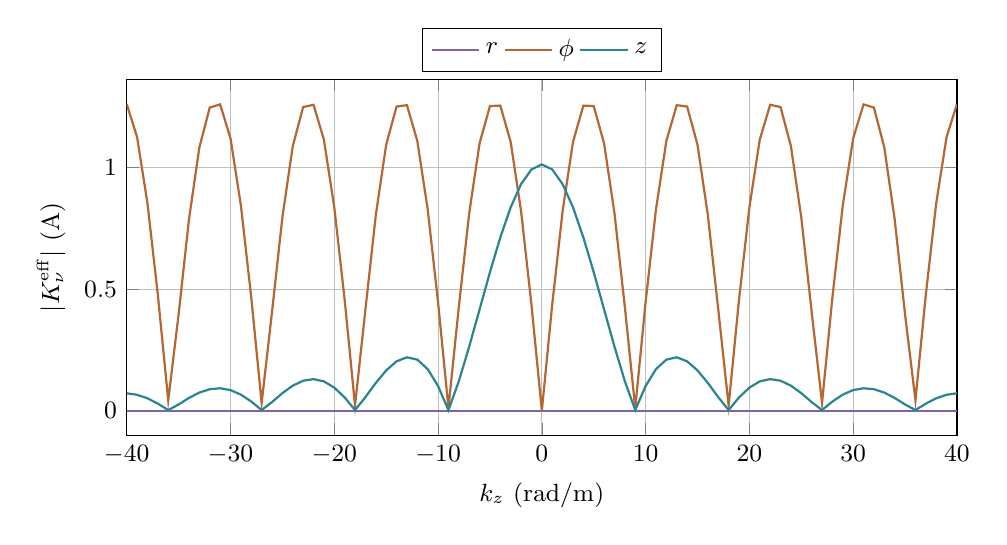
\begin{tikzpicture}
\begin{axis}[width=\linewidth,height=6.1cm,grid=major,
xlabel={$k_z$ (rad/m)},ylabel={$|K^{\rm eff}_\nu|$ (A)},
tick label style={font=\small},label style={font=\small},
legend style={font=\small,at={(.5,1.02)},anchor=south,legend columns=3},
xmin=-40,xmax=40,enlarge y limits=.08]
\addplot[violet,thick,no marks] coordinates {(-40,0) (-39,0) (-38,0) (-37,0) (-36,0) (-35,0) (-34,0) (-33,0) (-32,0) (-31,0) (-30,0) (-29,0) (-28,0) (-27,0) (-26,0) (-25,0) (-24,0) (-23,0) (-22,0) (-21,0) (-20,0) (-19,0) (-18,0) (-17,0) (-16,0) (-15,0) (-14,0) (-13,0) (-12,0) (-11,0) (-10,0) (-9,0) (-8,0) (-7,0) (-6,0) (-5,0) (-4,0) (-3,0) (-2,0) (-1,0) (0,0) (1,0) (2,0) (3,0) (4,0) (5,0) (6,0) (7,0) (8,0) (9,0) (10,0) (11,0) (12,0) (13,0) (14,0) (15,0) (16,0) (17,0) (18,0) (19,0) (20,0) (21,0) (22,0) (23,0) (24,0) (25,0) (26,0) (27,0) (28,0) (29,0) (30,0) (31,0) (32,0) (33,0) (34,0) (35,0) (36,0) (37,0) (38,0) (39,0) (40,0)};
\addlegendentry{$r$}
\addplot[copper,thick,no marks] coordinates {(-40,1.26084617822) (-39,1.1247268046) (-38,0.852229161091) (-37,0.476394833439) (-36,0.0427954530572) (-35,0.395993071767) (-34,0.786765625247) (-33,1.08213924776) (-32,1.24629853645) (-31,1.25933842664) (-30,1.119677772) (-29,0.844251065763) (-28,0.466455055938) (-27,0.0320992368728) (-26,0.406148761495) (-25,0.795149364683) (-24,1.08773447015) (-23,1.24842679548) (-22,1.25774166117) (-21,1.11454959715) (-20,0.836213296188) (-19,0.456482307967) (-18,0.0214007518163) (-17,0.416275743386) (-16,0.80347690053) (-15,1.09325280814) (-14,1.25046681188) (-13,1.25605599467) (-12,1.10934264253) (-11,0.828116420501) (-10,0.446477294431) (-9,0.0107007540891) (-8,0.426373301635) (-7,0.811747644174) (-6,1.09869387168) (-5,1.25241844148) (-4,1.2542815463) (-3,1.10405727617) (-2,0.819961011013) (-1,0.436440722516) (0,1.03412804064e-16) (1,0.436440722516) (2,0.819961011013) (3,1.10405727617) (4,1.2542815463) (5,1.25241844148) (6,1.09869387168) (7,0.811747644174) (8,0.426373301635) (9,0.0107007540891) (10,0.446477294431) (11,0.828116420501) (12,1.10934264253) (13,1.25605599467) (14,1.25046681188) (15,1.09325280814) (16,0.80347690053) (17,0.416275743386) (18,0.0214007518163) (19,0.456482307967) (20,0.836213296188) (21,1.11454959715) (22,1.25774166117) (23,1.24842679548) (24,1.08773447015) (25,0.795149364683) (26,0.406148761495) (27,0.0320992368728) (28,0.466455055938) (29,0.844251065763) (30,1.119677772) (31,1.25933842664) (32,1.24629853645) (33,1.08213924776) (34,0.786765625247) (35,0.395993071767) (36,0.0427954530572) (37,0.476394833439) (38,0.852229161091) (39,1.1247268046) (40,1.26084617822)};
\addlegendentry{$\phi$}
\addplot[teal,thick,no marks] coordinates {(-40,0.0716389873986) (-39,0.0655435200818) (-38,0.0509706436059) (-37,0.0292625819066) (-36,0.00270173314755) (-35,0.025713835829) (-34,0.0525912851101) (-33,0.0745274964021) (-32,0.0885155210543) (-31,0.092326864123) (-30,0.0848240736365) (-29,0.0661638766272) (-28,0.0378616116833) (-27,0.00270195596573) (-26,0.0355025141167) (-25,0.0722863058802) (-24,0.103005158158) (-23,0.123362331569) (-22,0.12993198979) (-21,0.120622250774) (-20,0.0950242382032) (-19,0.054603146886) (-18,0.00270211512832) (-17,0.0556518373511) (-16,0.114130241553) (-15,0.165644364869) (-14,0.202997859072) (-13,0.219590208859) (-12,0.210102773206) (-11,0.171098433988) (-10,0.101472112371) (-9,0.00270221062857) (-8,0.121128778874) (-7,0.263554429927) (-6,0.416171921089) (-5,0.569281109762) (-4,0.71265996949) (-3,0.836407027404) (-2,0.931773876151) (-1,0.99191073299) (0,1.01245545757) (1,0.99191073299) (2,0.931773876151) (3,0.836407027404) (4,0.71265996949) (5,0.569281109762) (6,0.416171921089) (7,0.263554429927) (8,0.121128778874) (9,0.00270221062857) (10,0.101472112371) (11,0.171098433988) (12,0.210102773206) (13,0.219590208859) (14,0.202997859072) (15,0.165644364869) (16,0.114130241553) (17,0.0556518373511) (18,0.00270211512832) (19,0.054603146886) (20,0.0950242382032) (21,0.120622250774) (22,0.12993198979) (23,0.123362331569) (24,0.103005158158) (25,0.0722863058802) (26,0.0355025141167) (27,0.00270195596573) (28,0.0378616116833) (29,0.0661638766272) (30,0.0848240736365) (31,0.092326864123) (32,0.0885155210543) (33,0.0745274964021) (34,0.0525912851101) (35,0.025713835829) (36,0.00270173314755) (37,0.0292625819066) (38,0.0509706436059) (39,0.0655435200818) (40,0.0716389873986)};
\addlegendentry{$z$}
\end{axis}\end{tikzpicture}}
\par\small 展示汇总谱，$m=1$；场加载保留各源半径。
\end{minipage}
% END GENERATED: prescribed_current_16
\end{center}

\subsection{圆柱蛇形给定电流（编号 17）}
将蛇形曲线贴到 $r=b$ 的展开面 $(b\phi,z)$ 上。
给定 $N\ge2$ 条横向段，每段弧长 $d>0$，相邻段轴向节距 $p>0$，
第 $j$ 段位于 $\zeta_j=[j-(N-1)/2]p$。
横向段交替沿正、负 $\phi$，再以 $+z$ 的连接段接到下一条横向段，构成一条连续开曲线。
其总长为 $S=Nd+(N-1)p$。
指定
\begin{equation}
 I(s)=I\ee^{\ii\beta_I s},\qquad 0\le s\le S,
\end{equation}
$\beta_I$ 是输入的\textbf{沿线电流相位梯度}（rad/m），可正、负或零，
不是从工作频率、介质或等离子体求出的传播常数。
$\beta_I=0$ 对应整条路径同相电流；两端仍保留端点电荷。
本模型中没有微带基板、地板、覆盖层及其回流分布。

第 $\ell$ 个直段或圆弧段的起点为 $(b,\phi_\ell,z_\ell)$，
增量为 $(0,\Delta\phi_\ell,\Delta z_\ell)$，长度
$a_\ell=\sqrt{(b\Delta\phi_\ell)^2+(\Delta z_\ell)^2}$，
起始累计弧长为 $s_\ell$。
将段参数 $t\in[0,1]$ 的线性相位直接积分，得到每段贡献
\begin{equation}\label{eq:meanderSegment}
 \begin{aligned}
 \mathbf K_\ell={}&\frac{CW_\phi}{2\pi b}
 \begin{pmatrix}0\\b\Delta\phi_\ell\\\Delta z_\ell\end{pmatrix}
 \ee^{\ii\beta_I(s_\ell+a_\ell/2)
 -\ii[m(\phi_\ell+\Delta\phi_\ell/2)+k_z(z_\ell+\Delta z_\ell/2)]}\\
 &\times\sinc\!\left(\frac{m\Delta\phi_\ell+k_z\Delta z_\ell-\beta_Ia_\ell}{2}\right),
 \qquad \mathbf K=\sum_\ell\mathbf K_\ell.
 \end{aligned}
\end{equation}
因此几何折返和电流沿线相位都影响谱峰；$\beta_I=0$ 时也不能忽略各段的有向线元。
\begin{center}% BEGIN GENERATED: prescribed_current_17
% Current geometry exported by C; arrows show instantaneous real current at t=0.
\begin{minipage}[t]{.48\linewidth}\centering\vspace{0pt}
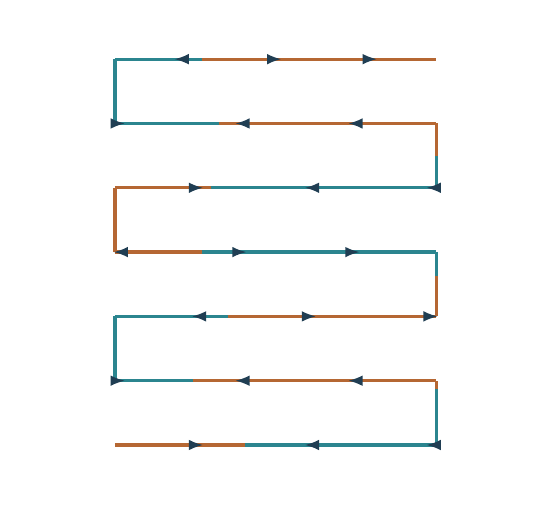
\begin{tikzpicture}[x=1cm,y=1cm,>=Latex,font=\small]
\path[use as bounding box] (-3.15,-2.85) rectangle (3.15,2.85);
\draw[copper,line width=1.15pt] (-2.04167,-2.45000)--(-1.93131,-2.45000);
\draw[copper,line width=1.15pt] (-1.93131,-2.45000)--(-1.82095,-2.45000);
\draw[copper,line width=1.15pt] (-1.82095,-2.45000)--(-1.71059,-2.45000);
\draw[copper,line width=1.15pt] (-1.71059,-2.45000)--(-1.60023,-2.45000);
\draw[copper,line width=1.15pt] (-1.60023,-2.45000)--(-1.48986,-2.45000);
\draw[copper,line width=1.15pt] (-1.48986,-2.45000)--(-1.37950,-2.45000);
\draw[copper,line width=1.15pt] (-1.37950,-2.45000)--(-1.26914,-2.45000);
\draw[copper,line width=1.15pt] (-1.26914,-2.45000)--(-1.15878,-2.45000);
\draw[copper,line width=1.15pt] (-1.15878,-2.45000)--(-1.04842,-2.45000);
\draw[copper,line width=1.15pt] (-1.04842,-2.45000)--(-0.93806,-2.45000);
\draw[copper,line width=1.15pt] (-0.93806,-2.45000)--(-0.82770,-2.45000);
\draw[copper,line width=1.15pt] (-0.82770,-2.45000)--(-0.71734,-2.45000);
\draw[copper,line width=1.15pt] (-0.71734,-2.45000)--(-0.60698,-2.45000);
\draw[copper,line width=1.15pt] (-0.60698,-2.45000)--(-0.49662,-2.45000);
\draw[copper,line width=1.15pt] (-0.49662,-2.45000)--(-0.38626,-2.45000);
\draw[teal,line width=1.15pt] (-0.38626,-2.45000)--(-0.27590,-2.45000);
\draw[teal,line width=1.15pt] (-0.27590,-2.45000)--(-0.16554,-2.45000);
\draw[teal,line width=1.15pt] (-0.16554,-2.45000)--(-0.05518,-2.45000);
\draw[teal,line width=1.15pt] (-0.05518,-2.45000)--(0.05518,-2.45000);
\draw[teal,line width=1.15pt] (0.05518,-2.45000)--(0.16554,-2.45000);
\draw[teal,line width=1.15pt] (0.16554,-2.45000)--(0.27590,-2.45000);
\draw[teal,line width=1.15pt] (0.27590,-2.45000)--(0.38626,-2.45000);
\draw[teal,line width=1.15pt] (0.38626,-2.45000)--(0.49662,-2.45000);
\draw[teal,line width=1.15pt] (0.49662,-2.45000)--(0.60698,-2.45000);
\draw[teal,line width=1.15pt] (0.60698,-2.45000)--(0.71734,-2.45000);
\draw[teal,line width=1.15pt] (0.71734,-2.45000)--(0.82770,-2.45000);
\draw[teal,line width=1.15pt] (0.82770,-2.45000)--(0.93806,-2.45000);
\draw[teal,line width=1.15pt] (0.93806,-2.45000)--(1.04842,-2.45000);
\draw[teal,line width=1.15pt] (1.04842,-2.45000)--(1.15878,-2.45000);
\draw[teal,line width=1.15pt] (1.15878,-2.45000)--(1.26914,-2.45000);
\draw[teal,line width=1.15pt] (1.26914,-2.45000)--(1.37950,-2.45000);
\draw[teal,line width=1.15pt] (1.37950,-2.45000)--(1.48986,-2.45000);
\draw[teal,line width=1.15pt] (1.48986,-2.45000)--(1.60023,-2.45000);
\draw[teal,line width=1.15pt] (1.60023,-2.45000)--(1.71059,-2.45000);
\draw[teal,line width=1.15pt] (1.71059,-2.45000)--(1.82095,-2.45000);
\draw[teal,line width=1.15pt] (1.82095,-2.45000)--(1.93131,-2.45000);
\draw[teal,line width=1.15pt] (1.93131,-2.45000)--(2.04167,-2.45000);
\draw[teal,line width=1.15pt] (2.04167,-2.45000)--(2.04167,-2.34792);
\draw[teal,line width=1.15pt] (2.04167,-2.34792)--(2.04167,-2.24583);
\draw[teal,line width=1.15pt] (2.04167,-2.24583)--(2.04167,-2.14375);
\draw[teal,line width=1.15pt] (2.04167,-2.14375)--(2.04167,-2.04167);
\draw[teal,line width=1.15pt] (2.04167,-2.04167)--(2.04167,-1.93958);
\draw[teal,line width=1.15pt] (2.04167,-1.93958)--(2.04167,-1.83750);
\draw[teal,line width=1.15pt] (2.04167,-1.83750)--(2.04167,-1.73542);
\draw[copper,line width=1.15pt] (2.04167,-1.73542)--(2.04167,-1.63333);
\draw[copper,line width=1.15pt] (2.04167,-1.63333)--(1.93131,-1.63333);
\draw[copper,line width=1.15pt] (1.93131,-1.63333)--(1.82095,-1.63333);
\draw[copper,line width=1.15pt] (1.82095,-1.63333)--(1.71059,-1.63333);
\draw[copper,line width=1.15pt] (1.71059,-1.63333)--(1.60023,-1.63333);
\draw[copper,line width=1.15pt] (1.60023,-1.63333)--(1.48986,-1.63333);
\draw[copper,line width=1.15pt] (1.48986,-1.63333)--(1.37950,-1.63333);
\draw[copper,line width=1.15pt] (1.37950,-1.63333)--(1.26914,-1.63333);
\draw[copper,line width=1.15pt] (1.26914,-1.63333)--(1.15878,-1.63333);
\draw[copper,line width=1.15pt] (1.15878,-1.63333)--(1.04842,-1.63333);
\draw[copper,line width=1.15pt] (1.04842,-1.63333)--(0.93806,-1.63333);
\draw[copper,line width=1.15pt] (0.93806,-1.63333)--(0.82770,-1.63333);
\draw[copper,line width=1.15pt] (0.82770,-1.63333)--(0.71734,-1.63333);
\draw[copper,line width=1.15pt] (0.71734,-1.63333)--(0.60698,-1.63333);
\draw[copper,line width=1.15pt] (0.60698,-1.63333)--(0.49662,-1.63333);
\draw[copper,line width=1.15pt] (0.49662,-1.63333)--(0.38626,-1.63333);
\draw[copper,line width=1.15pt] (0.38626,-1.63333)--(0.27590,-1.63333);
\draw[copper,line width=1.15pt] (0.27590,-1.63333)--(0.16554,-1.63333);
\draw[copper,line width=1.15pt] (0.16554,-1.63333)--(0.05518,-1.63333);
\draw[copper,line width=1.15pt] (0.05518,-1.63333)--(-0.05518,-1.63333);
\draw[copper,line width=1.15pt] (-0.05518,-1.63333)--(-0.16554,-1.63333);
\draw[copper,line width=1.15pt] (-0.16554,-1.63333)--(-0.27590,-1.63333);
\draw[copper,line width=1.15pt] (-0.27590,-1.63333)--(-0.38626,-1.63333);
\draw[copper,line width=1.15pt] (-0.38626,-1.63333)--(-0.49662,-1.63333);
\draw[copper,line width=1.15pt] (-0.49662,-1.63333)--(-0.60698,-1.63333);
\draw[copper,line width=1.15pt] (-0.60698,-1.63333)--(-0.71734,-1.63333);
\draw[copper,line width=1.15pt] (-0.71734,-1.63333)--(-0.82770,-1.63333);
\draw[copper,line width=1.15pt] (-0.82770,-1.63333)--(-0.93806,-1.63333);
\draw[copper,line width=1.15pt] (-0.93806,-1.63333)--(-1.04842,-1.63333);
\draw[teal,line width=1.15pt] (-1.04842,-1.63333)--(-1.15878,-1.63333);
\draw[teal,line width=1.15pt] (-1.15878,-1.63333)--(-1.26914,-1.63333);
\draw[teal,line width=1.15pt] (-1.26914,-1.63333)--(-1.37950,-1.63333);
\draw[teal,line width=1.15pt] (-1.37950,-1.63333)--(-1.48986,-1.63333);
\draw[teal,line width=1.15pt] (-1.48986,-1.63333)--(-1.60023,-1.63333);
\draw[teal,line width=1.15pt] (-1.60023,-1.63333)--(-1.71059,-1.63333);
\draw[teal,line width=1.15pt] (-1.71059,-1.63333)--(-1.82095,-1.63333);
\draw[teal,line width=1.15pt] (-1.82095,-1.63333)--(-1.93131,-1.63333);
\draw[teal,line width=1.15pt] (-1.93131,-1.63333)--(-2.04167,-1.63333);
\draw[teal,line width=1.15pt] (-2.04167,-1.63333)--(-2.04167,-1.53125);
\draw[teal,line width=1.15pt] (-2.04167,-1.53125)--(-2.04167,-1.42917);
\draw[teal,line width=1.15pt] (-2.04167,-1.42917)--(-2.04167,-1.32708);
\draw[teal,line width=1.15pt] (-2.04167,-1.32708)--(-2.04167,-1.22500);
\draw[teal,line width=1.15pt] (-2.04167,-1.22500)--(-2.04167,-1.12292);
\draw[teal,line width=1.15pt] (-2.04167,-1.12292)--(-2.04167,-1.02083);
\draw[teal,line width=1.15pt] (-2.04167,-1.02083)--(-2.04167,-0.91875);
\draw[teal,line width=1.15pt] (-2.04167,-0.91875)--(-2.04167,-0.81667);
\draw[teal,line width=1.15pt] (-2.04167,-0.81667)--(-1.93131,-0.81667);
\draw[teal,line width=1.15pt] (-1.93131,-0.81667)--(-1.82095,-0.81667);
\draw[teal,line width=1.15pt] (-1.82095,-0.81667)--(-1.71059,-0.81667);
\draw[teal,line width=1.15pt] (-1.71059,-0.81667)--(-1.60023,-0.81667);
\draw[teal,line width=1.15pt] (-1.60023,-0.81667)--(-1.48986,-0.81667);
\draw[teal,line width=1.15pt] (-1.48986,-0.81667)--(-1.37950,-0.81667);
\draw[teal,line width=1.15pt] (-1.37950,-0.81667)--(-1.26914,-0.81667);
\draw[teal,line width=1.15pt] (-1.26914,-0.81667)--(-1.15878,-0.81667);
\draw[teal,line width=1.15pt] (-1.15878,-0.81667)--(-1.04842,-0.81667);
\draw[teal,line width=1.15pt] (-1.04842,-0.81667)--(-0.93806,-0.81667);
\draw[teal,line width=1.15pt] (-0.93806,-0.81667)--(-0.82770,-0.81667);
\draw[teal,line width=1.15pt] (-0.82770,-0.81667)--(-0.71734,-0.81667);
\draw[teal,line width=1.15pt] (-0.71734,-0.81667)--(-0.60698,-0.81667);
\draw[copper,line width=1.15pt] (-0.60698,-0.81667)--(-0.49662,-0.81667);
\draw[copper,line width=1.15pt] (-0.49662,-0.81667)--(-0.38626,-0.81667);
\draw[copper,line width=1.15pt] (-0.38626,-0.81667)--(-0.27590,-0.81667);
\draw[copper,line width=1.15pt] (-0.27590,-0.81667)--(-0.16554,-0.81667);
\draw[copper,line width=1.15pt] (-0.16554,-0.81667)--(-0.05518,-0.81667);
\draw[copper,line width=1.15pt] (-0.05518,-0.81667)--(0.05518,-0.81667);
\draw[copper,line width=1.15pt] (0.05518,-0.81667)--(0.16554,-0.81667);
\draw[copper,line width=1.15pt] (0.16554,-0.81667)--(0.27590,-0.81667);
\draw[copper,line width=1.15pt] (0.27590,-0.81667)--(0.38626,-0.81667);
\draw[copper,line width=1.15pt] (0.38626,-0.81667)--(0.49662,-0.81667);
\draw[copper,line width=1.15pt] (0.49662,-0.81667)--(0.60698,-0.81667);
\draw[copper,line width=1.15pt] (0.60698,-0.81667)--(0.71734,-0.81667);
\draw[copper,line width=1.15pt] (0.71734,-0.81667)--(0.82770,-0.81667);
\draw[copper,line width=1.15pt] (0.82770,-0.81667)--(0.93806,-0.81667);
\draw[copper,line width=1.15pt] (0.93806,-0.81667)--(1.04842,-0.81667);
\draw[copper,line width=1.15pt] (1.04842,-0.81667)--(1.15878,-0.81667);
\draw[copper,line width=1.15pt] (1.15878,-0.81667)--(1.26914,-0.81667);
\draw[copper,line width=1.15pt] (1.26914,-0.81667)--(1.37950,-0.81667);
\draw[copper,line width=1.15pt] (1.37950,-0.81667)--(1.48986,-0.81667);
\draw[copper,line width=1.15pt] (1.48986,-0.81667)--(1.60023,-0.81667);
\draw[copper,line width=1.15pt] (1.60023,-0.81667)--(1.71059,-0.81667);
\draw[copper,line width=1.15pt] (1.71059,-0.81667)--(1.82095,-0.81667);
\draw[copper,line width=1.15pt] (1.82095,-0.81667)--(1.93131,-0.81667);
\draw[copper,line width=1.15pt] (1.93131,-0.81667)--(2.04167,-0.81667);
\draw[copper,line width=1.15pt] (2.04167,-0.81667)--(2.04167,-0.71458);
\draw[copper,line width=1.15pt] (2.04167,-0.71458)--(2.04167,-0.61250);
\draw[copper,line width=1.15pt] (2.04167,-0.61250)--(2.04167,-0.51042);
\draw[copper,line width=1.15pt] (2.04167,-0.51042)--(2.04167,-0.40833);
\draw[copper,line width=1.15pt] (2.04167,-0.40833)--(2.04167,-0.30625);
\draw[teal,line width=1.15pt] (2.04167,-0.30625)--(2.04167,-0.20417);
\draw[teal,line width=1.15pt] (2.04167,-0.20417)--(2.04167,-0.10208);
\draw[teal,line width=1.15pt] (2.04167,-0.10208)--(2.04167,0.00000);
\draw[teal,line width=1.15pt] (2.04167,0.00000)--(1.93131,0.00000);
\draw[teal,line width=1.15pt] (1.93131,0.00000)--(1.82095,0.00000);
\draw[teal,line width=1.15pt] (1.82095,0.00000)--(1.71059,0.00000);
\draw[teal,line width=1.15pt] (1.71059,0.00000)--(1.60023,0.00000);
\draw[teal,line width=1.15pt] (1.60023,0.00000)--(1.48986,0.00000);
\draw[teal,line width=1.15pt] (1.48986,0.00000)--(1.37950,0.00000);
\draw[teal,line width=1.15pt] (1.37950,0.00000)--(1.26914,0.00000);
\draw[teal,line width=1.15pt] (1.26914,0.00000)--(1.15878,0.00000);
\draw[teal,line width=1.15pt] (1.15878,0.00000)--(1.04842,0.00000);
\draw[teal,line width=1.15pt] (1.04842,0.00000)--(0.93806,0.00000);
\draw[teal,line width=1.15pt] (0.93806,0.00000)--(0.82770,0.00000);
\draw[teal,line width=1.15pt] (0.82770,0.00000)--(0.71734,0.00000);
\draw[teal,line width=1.15pt] (0.71734,0.00000)--(0.60698,0.00000);
\draw[teal,line width=1.15pt] (0.60698,0.00000)--(0.49662,0.00000);
\draw[teal,line width=1.15pt] (0.49662,0.00000)--(0.38626,0.00000);
\draw[teal,line width=1.15pt] (0.38626,0.00000)--(0.27590,0.00000);
\draw[teal,line width=1.15pt] (0.27590,0.00000)--(0.16554,0.00000);
\draw[teal,line width=1.15pt] (0.16554,0.00000)--(0.05518,0.00000);
\draw[teal,line width=1.15pt] (0.05518,0.00000)--(-0.05518,0.00000);
\draw[teal,line width=1.15pt] (-0.05518,0.00000)--(-0.16554,0.00000);
\draw[teal,line width=1.15pt] (-0.16554,0.00000)--(-0.27590,0.00000);
\draw[teal,line width=1.15pt] (-0.27590,0.00000)--(-0.38626,0.00000);
\draw[teal,line width=1.15pt] (-0.38626,0.00000)--(-0.49662,0.00000);
\draw[teal,line width=1.15pt] (-0.49662,0.00000)--(-0.60698,0.00000);
\draw[teal,line width=1.15pt] (-0.60698,0.00000)--(-0.71734,0.00000);
\draw[teal,line width=1.15pt] (-0.71734,0.00000)--(-0.82770,0.00000);
\draw[teal,line width=1.15pt] (-0.82770,0.00000)--(-0.93806,0.00000);
\draw[copper,line width=1.15pt] (-0.93806,0.00000)--(-1.04842,0.00000);
\draw[copper,line width=1.15pt] (-1.04842,0.00000)--(-1.15878,0.00000);
\draw[copper,line width=1.15pt] (-1.15878,0.00000)--(-1.26914,0.00000);
\draw[copper,line width=1.15pt] (-1.26914,0.00000)--(-1.37950,0.00000);
\draw[copper,line width=1.15pt] (-1.37950,0.00000)--(-1.48986,0.00000);
\draw[copper,line width=1.15pt] (-1.48986,0.00000)--(-1.60023,0.00000);
\draw[copper,line width=1.15pt] (-1.60023,0.00000)--(-1.71059,0.00000);
\draw[copper,line width=1.15pt] (-1.71059,0.00000)--(-1.82095,0.00000);
\draw[copper,line width=1.15pt] (-1.82095,0.00000)--(-1.93131,0.00000);
\draw[copper,line width=1.15pt] (-1.93131,0.00000)--(-2.04167,0.00000);
\draw[copper,line width=1.15pt] (-2.04167,0.00000)--(-2.04167,0.10208);
\draw[copper,line width=1.15pt] (-2.04167,0.10208)--(-2.04167,0.20417);
\draw[copper,line width=1.15pt] (-2.04167,0.20417)--(-2.04167,0.30625);
\draw[copper,line width=1.15pt] (-2.04167,0.30625)--(-2.04167,0.40833);
\draw[copper,line width=1.15pt] (-2.04167,0.40833)--(-2.04167,0.51042);
\draw[copper,line width=1.15pt] (-2.04167,0.51042)--(-2.04167,0.61250);
\draw[copper,line width=1.15pt] (-2.04167,0.61250)--(-2.04167,0.71458);
\draw[copper,line width=1.15pt] (-2.04167,0.71458)--(-2.04167,0.81667);
\draw[copper,line width=1.15pt] (-2.04167,0.81667)--(-1.93131,0.81667);
\draw[copper,line width=1.15pt] (-1.93131,0.81667)--(-1.82095,0.81667);
\draw[copper,line width=1.15pt] (-1.82095,0.81667)--(-1.71059,0.81667);
\draw[copper,line width=1.15pt] (-1.71059,0.81667)--(-1.60023,0.81667);
\draw[copper,line width=1.15pt] (-1.60023,0.81667)--(-1.48986,0.81667);
\draw[copper,line width=1.15pt] (-1.48986,0.81667)--(-1.37950,0.81667);
\draw[copper,line width=1.15pt] (-1.37950,0.81667)--(-1.26914,0.81667);
\draw[copper,line width=1.15pt] (-1.26914,0.81667)--(-1.15878,0.81667);
\draw[copper,line width=1.15pt] (-1.15878,0.81667)--(-1.04842,0.81667);
\draw[copper,line width=1.15pt] (-1.04842,0.81667)--(-0.93806,0.81667);
\draw[copper,line width=1.15pt] (-0.93806,0.81667)--(-0.82770,0.81667);
\draw[teal,line width=1.15pt] (-0.82770,0.81667)--(-0.71734,0.81667);
\draw[teal,line width=1.15pt] (-0.71734,0.81667)--(-0.60698,0.81667);
\draw[teal,line width=1.15pt] (-0.60698,0.81667)--(-0.49662,0.81667);
\draw[teal,line width=1.15pt] (-0.49662,0.81667)--(-0.38626,0.81667);
\draw[teal,line width=1.15pt] (-0.38626,0.81667)--(-0.27590,0.81667);
\draw[teal,line width=1.15pt] (-0.27590,0.81667)--(-0.16554,0.81667);
\draw[teal,line width=1.15pt] (-0.16554,0.81667)--(-0.05518,0.81667);
\draw[teal,line width=1.15pt] (-0.05518,0.81667)--(0.05518,0.81667);
\draw[teal,line width=1.15pt] (0.05518,0.81667)--(0.16554,0.81667);
\draw[teal,line width=1.15pt] (0.16554,0.81667)--(0.27590,0.81667);
\draw[teal,line width=1.15pt] (0.27590,0.81667)--(0.38626,0.81667);
\draw[teal,line width=1.15pt] (0.38626,0.81667)--(0.49662,0.81667);
\draw[teal,line width=1.15pt] (0.49662,0.81667)--(0.60698,0.81667);
\draw[teal,line width=1.15pt] (0.60698,0.81667)--(0.71734,0.81667);
\draw[teal,line width=1.15pt] (0.71734,0.81667)--(0.82770,0.81667);
\draw[teal,line width=1.15pt] (0.82770,0.81667)--(0.93806,0.81667);
\draw[teal,line width=1.15pt] (0.93806,0.81667)--(1.04842,0.81667);
\draw[teal,line width=1.15pt] (1.04842,0.81667)--(1.15878,0.81667);
\draw[teal,line width=1.15pt] (1.15878,0.81667)--(1.26914,0.81667);
\draw[teal,line width=1.15pt] (1.26914,0.81667)--(1.37950,0.81667);
\draw[teal,line width=1.15pt] (1.37950,0.81667)--(1.48986,0.81667);
\draw[teal,line width=1.15pt] (1.48986,0.81667)--(1.60023,0.81667);
\draw[teal,line width=1.15pt] (1.60023,0.81667)--(1.71059,0.81667);
\draw[teal,line width=1.15pt] (1.71059,0.81667)--(1.82095,0.81667);
\draw[teal,line width=1.15pt] (1.82095,0.81667)--(1.93131,0.81667);
\draw[teal,line width=1.15pt] (1.93131,0.81667)--(2.04167,0.81667);
\draw[teal,line width=1.15pt] (2.04167,0.81667)--(2.04167,0.91875);
\draw[teal,line width=1.15pt] (2.04167,0.91875)--(2.04167,1.02083);
\draw[teal,line width=1.15pt] (2.04167,1.02083)--(2.04167,1.12292);
\draw[teal,line width=1.15pt] (2.04167,1.12292)--(2.04167,1.22500);
\draw[copper,line width=1.15pt] (2.04167,1.22500)--(2.04167,1.32708);
\draw[copper,line width=1.15pt] (2.04167,1.32708)--(2.04167,1.42917);
\draw[copper,line width=1.15pt] (2.04167,1.42917)--(2.04167,1.53125);
\draw[copper,line width=1.15pt] (2.04167,1.53125)--(2.04167,1.63333);
\draw[copper,line width=1.15pt] (2.04167,1.63333)--(1.93131,1.63333);
\draw[copper,line width=1.15pt] (1.93131,1.63333)--(1.82095,1.63333);
\draw[copper,line width=1.15pt] (1.82095,1.63333)--(1.71059,1.63333);
\draw[copper,line width=1.15pt] (1.71059,1.63333)--(1.60023,1.63333);
\draw[copper,line width=1.15pt] (1.60023,1.63333)--(1.48986,1.63333);
\draw[copper,line width=1.15pt] (1.48986,1.63333)--(1.37950,1.63333);
\draw[copper,line width=1.15pt] (1.37950,1.63333)--(1.26914,1.63333);
\draw[copper,line width=1.15pt] (1.26914,1.63333)--(1.15878,1.63333);
\draw[copper,line width=1.15pt] (1.15878,1.63333)--(1.04842,1.63333);
\draw[copper,line width=1.15pt] (1.04842,1.63333)--(0.93806,1.63333);
\draw[copper,line width=1.15pt] (0.93806,1.63333)--(0.82770,1.63333);
\draw[copper,line width=1.15pt] (0.82770,1.63333)--(0.71734,1.63333);
\draw[copper,line width=1.15pt] (0.71734,1.63333)--(0.60698,1.63333);
\draw[copper,line width=1.15pt] (0.60698,1.63333)--(0.49662,1.63333);
\draw[copper,line width=1.15pt] (0.49662,1.63333)--(0.38626,1.63333);
\draw[copper,line width=1.15pt] (0.38626,1.63333)--(0.27590,1.63333);
\draw[copper,line width=1.15pt] (0.27590,1.63333)--(0.16554,1.63333);
\draw[copper,line width=1.15pt] (0.16554,1.63333)--(0.05518,1.63333);
\draw[copper,line width=1.15pt] (0.05518,1.63333)--(-0.05518,1.63333);
\draw[copper,line width=1.15pt] (-0.05518,1.63333)--(-0.16554,1.63333);
\draw[copper,line width=1.15pt] (-0.16554,1.63333)--(-0.27590,1.63333);
\draw[copper,line width=1.15pt] (-0.27590,1.63333)--(-0.38626,1.63333);
\draw[copper,line width=1.15pt] (-0.38626,1.63333)--(-0.49662,1.63333);
\draw[copper,line width=1.15pt] (-0.49662,1.63333)--(-0.60698,1.63333);
\draw[copper,line width=1.15pt] (-0.60698,1.63333)--(-0.71734,1.63333);
\draw[teal,line width=1.15pt] (-0.71734,1.63333)--(-0.82770,1.63333);
\draw[teal,line width=1.15pt] (-0.82770,1.63333)--(-0.93806,1.63333);
\draw[teal,line width=1.15pt] (-0.93806,1.63333)--(-1.04842,1.63333);
\draw[teal,line width=1.15pt] (-1.04842,1.63333)--(-1.15878,1.63333);
\draw[teal,line width=1.15pt] (-1.15878,1.63333)--(-1.26914,1.63333);
\draw[teal,line width=1.15pt] (-1.26914,1.63333)--(-1.37950,1.63333);
\draw[teal,line width=1.15pt] (-1.37950,1.63333)--(-1.48986,1.63333);
\draw[teal,line width=1.15pt] (-1.48986,1.63333)--(-1.60023,1.63333);
\draw[teal,line width=1.15pt] (-1.60023,1.63333)--(-1.71059,1.63333);
\draw[teal,line width=1.15pt] (-1.71059,1.63333)--(-1.82095,1.63333);
\draw[teal,line width=1.15pt] (-1.82095,1.63333)--(-1.93131,1.63333);
\draw[teal,line width=1.15pt] (-1.93131,1.63333)--(-2.04167,1.63333);
\draw[teal,line width=1.15pt] (-2.04167,1.63333)--(-2.04167,1.73542);
\draw[teal,line width=1.15pt] (-2.04167,1.73542)--(-2.04167,1.83750);
\draw[teal,line width=1.15pt] (-2.04167,1.83750)--(-2.04167,1.93958);
\draw[teal,line width=1.15pt] (-2.04167,1.93958)--(-2.04167,2.04167);
\draw[teal,line width=1.15pt] (-2.04167,2.04167)--(-2.04167,2.14375);
\draw[teal,line width=1.15pt] (-2.04167,2.14375)--(-2.04167,2.24583);
\draw[teal,line width=1.15pt] (-2.04167,2.24583)--(-2.04167,2.34792);
\draw[teal,line width=1.15pt] (-2.04167,2.34792)--(-2.04167,2.45000);
\draw[teal,line width=1.15pt] (-2.04167,2.45000)--(-1.93131,2.45000);
\draw[teal,line width=1.15pt] (-1.93131,2.45000)--(-1.82095,2.45000);
\draw[teal,line width=1.15pt] (-1.82095,2.45000)--(-1.71059,2.45000);
\draw[teal,line width=1.15pt] (-1.71059,2.45000)--(-1.60023,2.45000);
\draw[teal,line width=1.15pt] (-1.60023,2.45000)--(-1.48986,2.45000);
\draw[teal,line width=1.15pt] (-1.48986,2.45000)--(-1.37950,2.45000);
\draw[teal,line width=1.15pt] (-1.37950,2.45000)--(-1.26914,2.45000);
\draw[teal,line width=1.15pt] (-1.26914,2.45000)--(-1.15878,2.45000);
\draw[teal,line width=1.15pt] (-1.15878,2.45000)--(-1.04842,2.45000);
\draw[teal,line width=1.15pt] (-1.04842,2.45000)--(-0.93806,2.45000);
\draw[copper,line width=1.15pt] (-0.93806,2.45000)--(-0.82770,2.45000);
\draw[copper,line width=1.15pt] (-0.82770,2.45000)--(-0.71734,2.45000);
\draw[copper,line width=1.15pt] (-0.71734,2.45000)--(-0.60698,2.45000);
\draw[copper,line width=1.15pt] (-0.60698,2.45000)--(-0.49662,2.45000);
\draw[copper,line width=1.15pt] (-0.49662,2.45000)--(-0.38626,2.45000);
\draw[copper,line width=1.15pt] (-0.38626,2.45000)--(-0.27590,2.45000);
\draw[copper,line width=1.15pt] (-0.27590,2.45000)--(-0.16554,2.45000);
\draw[copper,line width=1.15pt] (-0.16554,2.45000)--(-0.05518,2.45000);
\draw[copper,line width=1.15pt] (-0.05518,2.45000)--(0.05518,2.45000);
\draw[copper,line width=1.15pt] (0.05518,2.45000)--(0.16554,2.45000);
\draw[copper,line width=1.15pt] (0.16554,2.45000)--(0.27590,2.45000);
\draw[copper,line width=1.15pt] (0.27590,2.45000)--(0.38626,2.45000);
\draw[copper,line width=1.15pt] (0.38626,2.45000)--(0.49662,2.45000);
\draw[copper,line width=1.15pt] (0.49662,2.45000)--(0.60698,2.45000);
\draw[copper,line width=1.15pt] (0.60698,2.45000)--(0.71734,2.45000);
\draw[copper,line width=1.15pt] (0.71734,2.45000)--(0.82770,2.45000);
\draw[copper,line width=1.15pt] (0.82770,2.45000)--(0.93806,2.45000);
\draw[copper,line width=1.15pt] (0.93806,2.45000)--(1.04842,2.45000);
\draw[copper,line width=1.15pt] (1.04842,2.45000)--(1.15878,2.45000);
\draw[copper,line width=1.15pt] (1.15878,2.45000)--(1.26914,2.45000);
\draw[copper,line width=1.15pt] (1.26914,2.45000)--(1.37950,2.45000);
\draw[copper,line width=1.15pt] (1.37950,2.45000)--(1.48986,2.45000);
\draw[copper,line width=1.15pt] (1.48986,2.45000)--(1.60023,2.45000);
\draw[copper,line width=1.15pt] (1.60023,2.45000)--(1.71059,2.45000);
\draw[copper,line width=1.15pt] (1.71059,2.45000)--(1.82095,2.45000);
\draw[copper,line width=1.15pt] (1.82095,2.45000)--(1.93131,2.45000);
\draw[copper,line width=1.15pt] (1.93131,2.45000)--(2.04167,2.45000);
\draw[navy,line width=.65pt,-{Latex[length=1.8mm]}] (-1.06324,-2.45000)--(-0.92324,-2.45000);
\draw[navy,line width=.65pt,-{Latex[length=1.8mm]}] (0.51144,-2.45000)--(0.37144,-2.45000);
\draw[navy,line width=.65pt,-{Latex[length=1.8mm]}] (2.05649,-2.45000)--(1.91649,-2.45000);
\draw[navy,line width=.65pt,-{Latex[length=1.8mm]}] (1.06324,-1.63333)--(0.92324,-1.63333);
\draw[navy,line width=.65pt,-{Latex[length=1.8mm]}] (-0.37144,-1.63333)--(-0.51144,-1.63333);
\draw[navy,line width=.65pt,-{Latex[length=1.8mm]}] (-2.05649,-1.63333)--(-1.91649,-1.63333);
\draw[navy,line width=.65pt,-{Latex[length=1.8mm]}] (-0.92324,-0.81667)--(-1.06324,-0.81667);
\draw[navy,line width=.65pt,-{Latex[length=1.8mm]}] (0.37144,-0.81667)--(0.51144,-0.81667);
\draw[navy,line width=.65pt,-{Latex[length=1.8mm]}] (1.91649,-0.81667)--(2.05649,-0.81667);
\draw[navy,line width=.65pt,-{Latex[length=1.8mm]}] (0.92324,0.00000)--(1.06324,0.00000);
\draw[navy,line width=.65pt,-{Latex[length=1.8mm]}] (-0.51144,0.00000)--(-0.37144,0.00000);
\draw[navy,line width=.65pt,-{Latex[length=1.8mm]}] (-1.91649,0.00000)--(-2.05649,0.00000);
\draw[navy,line width=.65pt,-{Latex[length=1.8mm]}] (-1.06324,0.81667)--(-0.92324,0.81667);
\draw[navy,line width=.65pt,-{Latex[length=1.8mm]}] (0.51144,0.81667)--(0.37144,0.81667);
\draw[navy,line width=.65pt,-{Latex[length=1.8mm]}] (2.05649,0.81667)--(1.91649,0.81667);
\draw[navy,line width=.65pt,-{Latex[length=1.8mm]}] (1.06324,1.63333)--(0.92324,1.63333);
\draw[navy,line width=.65pt,-{Latex[length=1.8mm]}] (-0.37144,1.63333)--(-0.51144,1.63333);
\draw[navy,line width=.65pt,-{Latex[length=1.8mm]}] (-2.05649,1.63333)--(-1.91649,1.63333);
\draw[navy,line width=.65pt,-{Latex[length=1.8mm]}] (-1.14396,2.45000)--(-1.28396,2.45000);
\draw[navy,line width=.65pt,-{Latex[length=1.8mm]}] (-0.07000,2.45000)--(0.07000,2.45000);
\draw[navy,line width=.65pt,-{Latex[length=1.8mm]}] (1.14396,2.45000)--(1.28396,2.45000);
\end{tikzpicture}
\par\small 蛇形圆柱展开面：横向为 $b\phi$，竖向为 $z$
\end{minipage}\hfill
\begin{minipage}[t]{.50\linewidth}\centering\vspace{0pt}
\resizebox{\linewidth}{!}{%
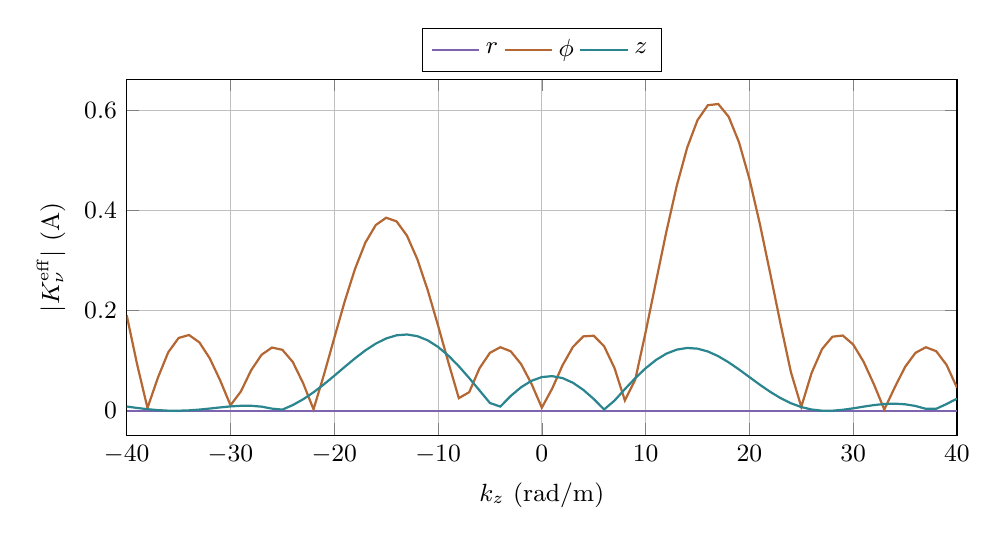
\begin{tikzpicture}
\begin{axis}[width=\linewidth,height=6.1cm,grid=major,
xlabel={$k_z$ (rad/m)},ylabel={$|K^{\rm eff}_\nu|$ (A)},
tick label style={font=\small},label style={font=\small},
legend style={font=\small,at={(.5,1.02)},anchor=south,legend columns=3},
xmin=-40,xmax=40,enlarge y limits=.08]
\addplot[violet,thick,no marks] coordinates {(-40,0) (-39,0) (-38,0) (-37,0) (-36,0) (-35,0) (-34,0) (-33,0) (-32,0) (-31,0) (-30,0) (-29,0) (-28,0) (-27,0) (-26,0) (-25,0) (-24,0) (-23,0) (-22,0) (-21,0) (-20,0) (-19,0) (-18,0) (-17,0) (-16,0) (-15,0) (-14,0) (-13,0) (-12,0) (-11,0) (-10,0) (-9,0) (-8,0) (-7,0) (-6,0) (-5,0) (-4,0) (-3,0) (-2,0) (-1,0) (0,0) (1,0) (2,0) (3,0) (4,0) (5,0) (6,0) (7,0) (8,0) (9,0) (10,0) (11,0) (12,0) (13,0) (14,0) (15,0) (16,0) (17,0) (18,0) (19,0) (20,0) (21,0) (22,0) (23,0) (24,0) (25,0) (26,0) (27,0) (28,0) (29,0) (30,0) (31,0) (32,0) (33,0) (34,0) (35,0) (36,0) (37,0) (38,0) (39,0) (40,0)};
\addlegendentry{$r$}
\addplot[copper,thick,no marks] coordinates {(-40,0.190410842727) (-39,0.0927200623501) (-38,0.005470052188) (-37,0.0656870459852) (-36,0.116659332959) (-35,0.145235868346) (-34,0.151239826056) (-33,0.136501685847) (-32,0.104656033449) (-31,0.0607811565382) (-30,0.0109144888117) (-29,0.0385121616169) (-28,0.0812667242284) (-27,0.111887059794) (-26,0.126176352643) (-25,0.121579731336) (-24,0.0974089711999) (-23,0.0548958913025) (-22,0.00292948335573) (-21,0.0715241531808) (-20,0.145254257891) (-19,0.217915306147) (-18,0.283303007472) (-17,0.335782735955) (-16,0.370805882673) (-15,0.385326240921) (-14,0.378078672152) (-13,0.349694800512) (-12,0.30264525482) (-11,0.241013690264) (-10,0.170123065102) (-9,0.0960480492519) (-8,0.025057796193) (-7,0.0369603158928) (-6,0.0850435493221) (-5,0.115613759331) (-4,0.126812287696) (-3,0.118678835629) (-2,0.0931573499845) (-1,0.0539275123825) (0,0.0060761428281) (1,0.0443626922106) (2,0.0909581425707) (3,0.127474566484) (4,0.148452063324) (5,0.149723342926) (6,0.128820183108) (7,0.0852323758619) (8,0.0204950513463) (9,0.0619045552175) (10,0.156793814627) (11,0.257732387171) (12,0.357544908884) (13,0.448922410837) (14,0.525039986203) (15,0.580136646691) (16,0.610006524103) (17,0.612358293015) (18,0.587011234773) (19,0.535910708307) (20,0.462961667639) (21,0.373694860952) (22,0.274795042733) (23,0.173532625254) (24,0.0771486168498) (25,0.00775330264733) (26,0.0757544855927) (27,0.123061178722) (28,0.147798591947) (29,0.150134231479) (30,0.132220744377) (31,0.097964536796) (32,0.0526418430454) (33,0.00239736644229) (34,0.0463291077503) (35,0.0873965218264) (36,0.115523586235) (37,0.126767025452) (38,0.118874628028) (39,0.0914820934901) (40,0.0461368056309)};
\addlegendentry{$\phi$}
\addplot[teal,thick,no marks] coordinates {(-40,0.00840164081061) (-39,0.00555624373973) (-38,0.0030656347212) (-37,0.00118748683324) (-36,0.000116550870558) (-35,4.1689570333e-05) (-34,0.000709260801979) (-33,0.00224603093235) (-32,0.00432490784279) (-31,0.00659249941754) (-30,0.00860734768715) (-29,0.00987135464983) (-28,0.00986898481737) (-27,0.00811143994398) (-26,0.00418243053992) (-25,0.0022181494959) (-24,0.0112363686787) (-23,0.0228356758529) (-22,0.0367804789885) (-21,0.0526339543372) (-20,0.0697711361866) (-19,0.0874071924563) (-18,0.104639607163) (-17,0.120501859505) (-16,0.13402520162) (-15,0.144304374796) (-14,0.150562633347) (-13,0.152211311715) (-12,0.1488993937) (-11,0.140549115698) (-10,0.127374524067) (-9,0.109881050445) (-8,0.0888454874786) (-7,0.0652771452738) (-6,0.0403623423405) (-5,0.0153956302362) (-4,0.00829782709744) (-3,0.0294435803877) (-2,0.0468974338154) (-1,0.0597177390516) (0,0.067225422557) (1,0.0690475275) (2,0.0651411683359) (3,0.0557961465769) (4,0.0416159628167) (5,0.023478474058) (6,0.00247887554614) (7,0.020141072865) (8,0.0430726959945) (9,0.0650234405679) (10,0.0847976014048) (11,0.101369237857) (12,0.113942377902) (13,0.121994553875) (14,0.125300939485) (15,0.123937770396) (16,0.118265224844) (17,0.108891405269) (18,0.0966203889222) (19,0.0823884077806) (20,0.0671929975554) (21,0.0520203679614) (22,0.0377762657261) (23,0.0252252321253) (24,0.0149424313912) (25,0.00728120495405) (26,0.00235827052712) (27,5.71310110273e-05) (28,4.88901248994e-05) (29,0.00182839302937) (30,0.00476251599701) (31,0.00814659872914) (32,0.0112645040017) (33,0.0134476340758) (34,0.0141284361395) (35,0.0128844667709) (36,0.00946990952133) (37,0.00383248059889) (38,0.00388516962788) (39,0.0133592403352) (40,0.0241122747227)};
\addlegendentry{$z$}
\end{axis}\end{tikzpicture}}
\par\small 展示汇总谱，$m=1$；场加载保留各源半径。
\end{minipage}
% END GENERATED: prescribed_current_17
\end{center}

\subsection{参数、算法与新增验证}
五幅左图直接来自 C 的 \texttt{Geometry}，箭头按零整体相位、$t=0$ 的电流实部绘制，
铜色、青色表示两个符号，接近零幅值的段为灰色。
右图是同一源积分器输出的 $|K_r^{\rm eff}|,|K_\phi^{\rm eff}|,|K_z^{\rm eff}|$，
不是场谱或功率谱。代表输入统一为 $b=0.44$ m、$I_0=1$ A、
$\bandwidth=0.04$ m、$z_0=\theta_0=\varphi_0=0$。
\begin{center}\small
\begin{tabular}{@{}r p{.76\linewidth}@{}}\toprule
编号 & 图及示例工程使用的附加参数\\\midrule
13 & $N=2$，$p=0.18$ m，$\Delta=180^\circ$，分析 $m=0$。\\
14 & $a_s=0.12$ m，$n_s=4$，$\chi=+1$，分析 $m=1$。\\
15 & $N_r=4$，$a_s=0.14$ m，$g=12^\circ$，$q=1$ 余弦驻波，分析 $m=1$。\\
16 & $N=8$，$L=0.70$ m，$q=1$ 余弦驻波，分析 $m=1$。\\
17 & $N=7$，$d=0.50$ m，$p=0.10$ m，$\beta_I=8$ rad/m，分析 $m=1$。\\
\bottomrule\end{tabular}\end{center}
在 UI 中，$N,N_r$ 共用 \texttt{elements}，并按类型显示为环数、径向环数、轴向腿数或横向段数；
$p$ 用 \texttt{spacing}，$a_s$ 用 \texttt{inner\_radius}，$g$ 用 \texttt{gap\_angle\_deg}，
$q$ 用 \texttt{source\_mode}，电流分布用 \texttt{current\_pattern}，
$\beta_I$ 用 \texttt{current\_phase\_gradient}。
$q$ 改变源的分布；\texttt{selected\_m} 选择正在查看的谱分量，二者不能混为同一输入。

\textbf{算法。} 先按上述路径生成端点和复电流权重；蛇形段另存起点电流相位及段内相位增量。
固定半径且相位线性的段直接使用式\eqref{eq:meanderSegment}的指数乘 sinc 积分，
不以常数相位替代段内相位。跨半径的螺旋按 FEM 径向单元交点切段后采用 Gauss 积分。
展宽平均与路径积分共用 \texttt{geometry\_integrate\_source}。
展示时才除以参考半径 $b$ 汇总；真空、等离子体和全模式重构均使用完整逐半径源加载。
修改背景介质不会改变这些已经给定的天线电流谱。

\textbf{独立验证。} 17 类基础检查包含 $17\times84=1428$ 组源谱，
另对分段环、鸟笼的旋转相位分布各检查 84 组，总计 1596 组。
13、15--17 号与本节解析表达式对照；14 号参考在连续 Archimedean 曲线上作独立 Simpson 积分，
不使用生成器的段列表。检查覆盖零波数、正负 $m$、非零源展宽、整体反向、相位、旋转及平移。
新增源电荷还通过独立的测试函数分部积分核验，鸟笼另检查节点电流收支。
每类另做真空和有限碰撞等离子体场求解，总计 34 次，检查原系统残差与源供功、吸收功率收支。
这些验证针对给定源及场方程，不代表求得了实际馈电电流。
% END INLINE CHAPTER: prescribed_current_antennas


\section{径向馈线与闭合电流守恒}\label{sec:sourcecontinuity}
本节用分布导数验证编号 9--12 的馈线与回流共同满足式\eqref{eq:continuity}。汇集前三种基本径向源，以上标 $\mathrm{line}$、$\mathrm{partial}$、$\mathrm{half}$ 分别标记直弦、部分匝和半 Nagoya：
\begin{align}\label{eq:Jr}
 \widehat J_r^{\rm line}(r)&=-\frac{\ii I\sinc(k_z {\bandwidth}/2)}{\pi r}\sin[m\arccos(b/r)]\mathbf1_{b<r<c},\\
 \widehat J_r^{\rm partial}(r)&=-\frac{\ii I\sinc(k_z {\bandwidth}/2)}{\pi r}\sin(m\alpha/2)\mathbf1_{b<r<c},\\
 \widehat J_r^{\rm half}(r)&=-\frac{\ii I\sinc(m {\bandwidth}/(2b))}{\pi r}\sin(k_zL/2)\mathbf1_{b<r<c}.
\end{align}
本节三式均取参考位置 $\theta_0=z_0=0$；任意位置需统一乘 $\ee^{-\ii(m\theta_0+k_z z_0)}$。半匝阵列对第二行乘式\eqref{eq:halfarrayfactor}定义的 $\arrayfactor$。指标函数的径向导数为 $\partial_r\mathbf1_{b<r<c}=\delta(r-b)-\delta(r-c)$。

以部分匝为例，把径向馈线乘 $r$ 并求导，得到
\begin{align}
 \partial_r(r\widehat J_r)&=-\frac{\ii I\sinc(k_z {\bandwidth}/2)}{\pi}\sin(m\alpha/2)[\delta(r-b)-\delta(r-c)],\\
 \ii m\widehat J_\phi&=\frac{\ii I\sinc(k_z {\bandwidth}/2)m\alpha}{2\pi}\sinc(m\alpha/2)[\delta(r-b)-\delta(r-c)].
\end{align}
利用恒等式
\begin{equation}
 m\alpha\sinc(m\alpha/2)=2\sin(m\alpha/2),\qquad
 k_zL\sinc(k_zL/2)=2\sin(k_zL/2),
\end{equation}
前两式严格抵消。第二个恒等式同样使半 Nagoya 的 $\ii k_zr\widehat J_z$ 与径向馈线端点导数抵消。

直弦除了端点，还需对 $\arccos(b/r)$ 求导。对 $b<r<c$ 有 $\partial_r\arccos(b/r)=b/[r\sqrt{r^2-b^2}]$；代入第一行的径向导数，正好抵消直弦周向项 $\ii m\widehat J_{\phi,\rm chord}$。外侧回流的面源抵消 $r=c$ 端点项。各支路共同满足电流连续性式\eqref{eq:continuity}。

\section{有限宽度电流源的场方程加载}\label{sec:sourceloading}
本节把前述几何与电流谱落实为径向场方程的规定源，并给出与程序输入的对应关系。物理量、字段及单位列于下表。
\begin{center}\small
\begin{tabular}{@{}>{\raggedright\arraybackslash}p{.16\linewidth}>{\raggedright\arraybackslash}p{.27\linewidth}>{\raggedright\arraybackslash}p{.49\linewidth}@{}}
\toprule 物理量 & 程序字段 & 含义和输入单位\\\midrule
$I_0$ & \texttt{current} & 每个单元的峰值电流，A。\\
$\currentdirection$ & \texttt{current\_direction} & 电流方向系数，$\pm1$。\\
$N$ & \texttt{elements} & 独立闭合阵列单元数，整数。\\
$n_h,\chi$ & \texttt{turns}, \texttt{winding\_direction} & 螺旋匝数与绕向，均无量纲。\\
$d$ & \texttt{width} & 两腿中心弧距，m；不是金属带宽。\\
${\bandwidth}$ & \texttt{band\_width} & 薄带面宽度，m。\\
$b,L$ & \texttt{antenna\_radius}, \texttt{antenna\_length} & 天线参考半径和轴向跨度，m；直带的 $b$ 为直弦到轴的距离。\\
$c,R$ & \texttt{return\_radius}, \texttt{radius} & 外侧回流半径与圆管内半径，m。\\
$s,z_0$ & \texttt{spacing}, \texttt{axial\_offset} & 单元中心弧距与轴向偏移，m。\\
$\alpha$ & \texttt{arc\_angle\_deg} & 采用独立张角的模板之输入，度。\\
$\Delta$ & \texttt{phase\_step} & 单元规定电流相位差，界面输入度。\\
$\theta_0$ & \texttt{azimuth\_deg} & 几何位置角，界面输入度。\\
$\varphi_0$ & \texttt{global\_phase\_deg} & 整体规定电流相位，界面输入度。\\
$m,k_z$ & \texttt{selected\_m}, \texttt{kz} & 整数方位模数与轴向波数（rad/m）。\\
$f$ & \texttt{frequency\_mhz} & 界面输入 MHz；进入 $\omega=2\pi f$ 前乘 $10^6$ 得 Hz。\\
\bottomrule
\end{tabular}\end{center}
公式中的角度统一为弧度；界面度数乘 $\pi/180$ 后分别得到 $\Delta,\theta_0,\varphi_0$；独立张角模板的 $\alpha$ 也按此换算。

对前面定义的无量纲径向测试函数 $\mathbf v(r)$，Maxwell 弱形式中的源项单位为 V，直接写成
\begin{equation}\label{eq:sourceaction}
 \ii\omega\mu_0\int_0^R r\mathbf v(r)^*\cdot\widehat{\mathbf J}(r)\dd r.
\end{equation}
单面 $r=b$ 的贡献为
\begin{equation}
 \ii\omega\mu_0b\{v_\phi(b)^*K_\phi+v_z(b)^*K_z\}.
\end{equation}
多半径源分别在 $b,c$ 加载面贡献，并在 $b<r<c$ 积分径向与直弦源。各源按其实际半径与测试函数作用，具体见式\eqref{eq:halfload}；$\Keff$ 用于结果汇总。

\par\endgroup

\section{十七类天线的源谱与场求解重新核查}\label{sec:antennaRecheck}
本次核查使用当前 C11 计算内核，天线类型从 1 到 17 连续编号；6 为单鞍、7 为双鞍形、8 为 Nagoya III。程序中的枚举、界面目录、示例项目和本文编号一致。源谱的独立参考实现位于 \path{c_workbench/tests/antenna_catalogue_test.c}；它不调用几何构造器生成解析参考，而是直接计算本章的闭式表达式，或对薄线解析谱作独立的复合 Simpson 宽度平均。直带参考直接积分 Cartesian 直弦并加上外侧圆弧回流。

\textbf{源谱检查。} 每类依次取 $m=-3,-2,-1,0,1,2,3$，$k_z=-10,0,10$ rad/m，$\bandwidth=0,0.04$ m，并分别计算参考位置与改变方向、整体相位、方位和轴向位置后的源。基础检查共 $17\times7\times3\times2\times2=1428$ 组，另对分段环、鸟笼的旋转相位分布增加 168 组，合计 1596 组，对照完整的 $(K_r^{\mathrm{eff}},K_\phi^{\mathrm{eff}},K_z^{\mathrm{eff}})$；$m=0$、$k_z=0$ 和对称相消模式均直接包含。闭合模板另检查节点电流闭合；新增开曲线与沿线变相位电流按第~\ref{sec:prescribedFive}~节检查源电荷的弱连续性关系。双鞍形的反相关系、四腿方向及式\eqref{eq:saddleNagoyaLimit}另作专门检查。

\textbf{场与功率检查。} 代表输入为 $R=0.60$ m，$b=0.44$ m，$c=0.55$ m，$L=0.70$ m，$I_0=1$ A，$\bandwidth=0.04$ m，$f=13.56$ MHz，$k_z=10$ rad/m。单环及轴向多环取 $m=0$，其余天线取 $m=1$；每类各解一次真空及冷等离子体边值问题，共 34 次。新增五类的附加尺寸和电流参数见第~\ref{sec:prescribedFive}~节。等离子体取 $a=0.30$ m，$n_0=10^{16}$ m$^{-3}$，边缘密度比 0.20 的抛物线剖面，$B_0=0.02$ T，$\nu_e=5\times10^6$ s$^{-1}$、$\nu_i=10^4$ s$^{-1}$，氩离子质量 $39.948$ u。径向输入网格数为 256，内部网格按材料界面、源半径及波长自动加点。

单带取 $d=0.18$ m；两种矩形阵列取 $d=0.12$ m、$s=0.18$ m，多带为 $N=4,\Delta=90^\circ$，梳状为 $N=6,\Delta=75^\circ$。双臂螺旋取半匝、负绕向、整体方位 $90^\circ$；双鞍形取 $\alpha=120^\circ$，单鞍取 $120^\circ$，部分匝及半匝阵列的单元取 $180^\circ$，半匝阵列为 $N=4,\Delta=90^\circ$。每类仅使用其实际需要的参数。

下表的源谱误差是全部对应检查中 $\max_\nu|K_{\nu,\text{计算}}-K_{\nu,\text{参考}}|/I_0$ 的最大值。$\eta_{\rm FEM}$ 取真空与等离子体两次求解中较大的原系统归一化残差；$\eta_P$ 为有限碰撞等离子体的 $|P_{\rm src}-P_{\rm abs}|/\max(|P_{\rm src}|,|P_{\rm abs}|)$。这些是当前计算输出，不以重新赋值强迫源供功等于吸收。
% BEGIN GENERATED: antenna_checks
% Generated from the current seventeen-model numerical audit.
\begin{center}\small
\begin{tabular}{@{}r l r r r@{}}\toprule
编号 & 天线 & $\max|\Delta K|/I_0$ & $\eta_{\rm FEM}$ & $\eta_P$\\\midrule
1 & 单带 & $1.94\times10^{-15}$ & $1.39\times10^{-16}$ & $1.66\times10^{-12}$\\
2 & 多带阵列 & $7.07\times10^{-15}$ & $1.51\times10^{-16}$ & $2.24\times10^{-11}$\\
3 & 梳状阵列 & $1.14\times10^{-14}$ & $1.33\times10^{-16}$ & $2.92\times10^{-12}$\\
4 & 全匝圆环 & $1.59\times10^{-14}$ & $1.06\times10^{-16}$ & $1.05\times10^{-11}$\\
5 & 双臂螺旋 & $1.10\times10^{-14}$ & $1.70\times10^{-16}$ & $6.31\times10^{-12}$\\
6 & 单鞍 & $2.45\times10^{-15}$ & $1.64\times10^{-16}$ & $3.04\times10^{-12}$\\
7 & 双鞍形 & $2.99\times10^{-15}$ & $1.66\times10^{-16}$ & $7.68\times10^{-12}$\\
8 & Nagoya III & $8.29\times10^{-15}$ & $2.01\times10^{-16}$ & $6.54\times10^{-12}$\\
9 & 直带与回流 & $9.21\times10^{-16}$ & $1.99\times10^{-16}$ & $7.71\times10^{-12}$\\
10 & 部分匝 & $6.80\times10^{-15}$ & $1.36\times10^{-16}$ & $2.17\times10^{-11}$\\
11 & 半 Nagoya & $7.84\times10^{-16}$ & $3.02\times10^{-16}$ & $4.46\times10^{-12}$\\
12 & 半匝阵列 & $3.58\times10^{-14}$ & $1.63\times10^{-16}$ & $1.85\times10^{-12}$\\
13 & 轴向多环 & $2.18\times10^{-14}$ & $1.81\times10^{-16}$ & $2.49\times10^{-12}$\\
14 & 平面螺旋 & $1.54\times10^{-12}$ & $2.14\times10^{-16}$ & $4.76\times10^{-12}$\\
15 & 分段多环 & $4.64\times10^{-15}$ & $1.86\times10^{-16}$ & $1.86\times10^{-11}$\\
16 & 鸟笼电流 & $2.66\times10^{-15}$ & $2.01\times10^{-16}$ & $6.07\times10^{-12}$\\
17 & 蛇形电流 & $2.37\times10^{-15}$ & $3.01\times10^{-16}$ & $9.00\times10^{-10}$\\
\bottomrule\end{tabular}
\end{center}
% END GENERATED: antenna_checks

全部独立谱检查的归一化误差小于 $2\times10^{-12}$，34 次求解的最大原系统残差小于 $4\times10^{-16}$，最大有功收支误差小于 $10^{-8}$。这些检查核对规定源及当前离散问题；极小代数残差不能代替网格、谱截断和碰撞参数的收敛检查。后续章节继续说明相应离散误差及适用范围。

下一章以本章的完整规定源建立真空径向边值问题。

\chapter{真空场}\label{chap:vacuum}

第一章已经把天线写成给定的复电流源；闭合回路满足零散度，开曲线及变相位路径的源电荷由连续性方程确定。本章固定驱动角频率 $\omega$、方位模式数 $m$ 和轴向波数 $k_z$，将源代入真空 Maxwell 方程，求解 $0\le r\le R$ 上的径向边值问题。先建立强形式与边界条件，再构造相容有限元和解析参考，最后说明复场恢复及物理代码的执行顺序。

\section{真空径向 Maxwell 方程的推导}
\label{sec:radialmaxwell}
单圆柱带面由 $K_\phi,K_z$ 加载；多半径天线使用 $\widehat{\mathbf J}(r)$ 的完整径向分布。两者服从同一组矢量 Maxwell 方程，差别集中在源项。

\subsection{时间约定与 Maxwell 方程}
沿用第一章的峰值相量，真实电场为 $\operatorname{Re}[\mathbf E(\mathbf x)\ee^{-\ii\omega t}]$，因此 $\partial_t\mapsto-\ii\omega$。真空中 $\mathbf D=\epsilon_0\mathbf E$、$\mathbf H=\mathbf B/\mu_0$，其中 $\mathbf D$ 为电位移（C/m$^2$），$\mathbf H$ 为磁场强度（A/m）；其余场量与常数的定义见第~\ref{sec:conventions}~节。由 Maxwell 方程出发：
\begin{align}
 \nabla\times\mathbf E&=-\partial_t\mathbf B=\ii\omega\mathbf B,\\
 \nabla\times\mathbf B&=\mu_0\mathbf J+\mu_0\epsilon_0\partial_t\mathbf E
 =\mu_0\mathbf J-\ii\omega\mu_0\epsilon_0\mathbf E.
\end{align}
对第一式再取旋度，并代入第二式：
\begin{align}
 \nabla\times\nabla\times\mathbf E
 &=\ii\omega(\mu_0\mathbf J-\ii\omega\mu_0\epsilon_0\mathbf E)\\
 &=\ii\omega\mu_0\mathbf J+\omega^2\mu_0\epsilon_0\mathbf E.
\end{align}
由于 $\ii(-\ii)=1$，令 $k_0=\omega/c_0=\omega\sqrt{\mu_0\epsilon_0}$，得到
\begin{equation}\label{eq:radialcurlcurl}
 \boxed{\nabla\times\nabla\times\mathbf E-k_0^2\mathbf E=\ii\omega\mu_0\mathbf J.}
\end{equation}
$\omega=2\pi f$，其中 $f$ 为驱动频率（Hz），$\omega$ 为角频率（s$^{-1}$），$c_0=1/\sqrt{\epsilon_0\mu_0}$ 为真空光速（m/s），$k_0$ 为真空波数（m$^{-1}$）。程序将 MHz 输入乘 $10^6$ 后代入。

\subsection{只变换角向和轴向，保留半径}
对每个圆柱分量使用第一章的 Fourier 约定；$\nu\in\{r,\phi,z\}$ 是分量标签，$r,z$ 的单位为 m，$\phi$ 为方位角（rad）：
\begin{equation}
 \widehat E_\nu(r;m,k_z)=\int_{-\infty}^{\infty}\!\dd z
 \int_0^{2\pi}\!\frac{\dd\phi}{2\pi}\,
 E_\nu(r,\phi,z)\ee^{-\ii(m\phi+k_z z)}.
\end{equation}
分部积分给出 $\widehat{\partial_\phi E_\nu}=\ii m\widehat E_\nu$ 和
$\widehat{\partial_z E_\nu}=\ii k_z\widehat E_\nu$；对 $r$ 的导数保留。$m$ 是无量纲有符号整数，$k_z$ 是有符号连续波数（m$^{-1}$）。帽号均表示同一组 $(m,k_z)$ 的谱量。正变换中的轴向积分增加一个长度因子，所以 $\widehat E_\nu$、$\widehat B_\nu$、$\widehat J_\nu$ 的单位依次为 V、T$\cdot$m、A/m。

圆柱坐标的一次旋度完整写为
\begin{align}
 (\widehat{\nabla\times\mathbf E})_r
 &=\frac{\ii m}{r}\widehat E_z-\ii k_z\widehat E_\phi,\\
 (\widehat{\nabla\times\mathbf E})_\phi
 &=\ii k_z\widehat E_r-\frac{\dd\widehat E_z}{\dd r},\\
 (\widehat{\nabla\times\mathbf E})_z
 &=\frac{\dd\widehat E_\phi}{\dd r}+\frac{\widehat E_\phi}{r}
   -\frac{\ii m}{r}\widehat E_r.
\end{align}
其中 $\widehat E_\phi/r$ 来自圆柱基矢随位置转动，是圆柱旋度的几何项。

\subsection{再次取旋度：实际求解的强形式}
以下场谱上的撇号表示对半径 $r$ 求导，因而一阶、二阶电场谱导数的单位分别为 V/m、V/m$^2$。例如径向分量为
\begin{align}
 (\widehat{\nabla\times\nabla\times\mathbf E})_r
 ={}&\frac{\ii m}{r}\left(\widehat E_\phi'+\frac{\widehat E_\phi}{r}
 -\frac{\ii m}{r}\widehat E_r\right)
 -\ii k_z(\ii k_z\widehat E_r-\widehat E_z')\\
 ={}&\left(\frac{m^2}{r^2}+k_z^2\right)\widehat E_r
 +\frac{\ii m}{r}\widehat E_\phi'
 +\frac{\ii m}{r^2}\widehat E_\phi+\ii k_z\widehat E_z'.
\end{align}
周向和轴向分量在展开前分别为
\begin{align*}
 (\widehat{\nabla\times\nabla\times\mathbf E})_\phi
 &=\ii k_z\left(\frac{\ii m}{r}\widehat E_z-\ii k_z\widehat E_\phi\right)
 -\frac\dd{\dd r}\left(\widehat E_\phi'+\frac{\widehat E_\phi}{r}-\frac{\ii m}{r}\widehat E_r\right),\\
 (\widehat{\nabla\times\nabla\times\mathbf E})_z
 &=\frac1r\frac\dd{\dd r}\left[r(\ii k_z\widehat E_r-\widehat E_z')\right]
 -\frac{\ii m}{r}\left(\frac{\ii m}{r}\widehat E_z-\ii k_z\widehat E_\phi\right).
\end{align*}
分别使用乘积求导，并减去 $k_0^2\widehat E_\nu$，得到三个完全展开的方程：
\begin{equation}\label{eq:radialstrongr}
 \boxed{\left(\frac{m^2}{r^2}+k_z^2-k_0^2\right)\widehat E_r
 +\frac{\ii m}{r}\widehat E_\phi'
 +\frac{\ii m}{r^2}\widehat E_\phi+\ii k_z\widehat E_z'
 =\ii\omega\mu_0\widehat J_r.}
\end{equation}
\begin{equation}\label{eq:radialstrongphi}
 \boxed{\begin{aligned}
 -\widehat E_\phi''-\frac1r\widehat E_\phi'
 +\left(\frac1{r^2}+k_z^2-k_0^2\right)\widehat E_\phi
 &+\frac{\ii m}{r}\widehat E_r'-\frac{\ii m}{r^2}\widehat E_r\\
 &-\frac{mk_z}{r}\widehat E_z=\ii\omega\mu_0\widehat J_\phi.
 \end{aligned}}
\end{equation}
\begin{equation}\label{eq:radialstrongz}
 \boxed{\begin{aligned}
 -\widehat E_z''-\frac1r\widehat E_z'
 +\left(\frac{m^2}{r^2}-k_0^2\right)\widehat E_z
 &+\ii k_z\widehat E_r'+\frac{\ii k_z}{r}\widehat E_r\\
 &-\frac{mk_z}{r}\widehat E_\phi=\ii\omega\mu_0\widehat J_z.
 \end{aligned}}
\end{equation}
这是一组关于 $r$ 的耦合方程：径向分量由第一式约束，周向、轴向分量含二阶径向导数。即使 $\widehat J_r=0$，分量间的耦合仍可产生非零 $\widehat E_r$。

\subsection{电流守恒何时允许化简为标量方程}
对式\eqref{eq:radialcurlcurl}取散度，利用旋度的散度为零：
\begin{equation}
 -k_0^2\nabla\cdot\mathbf E=\ii\omega\mu_0\nabla\cdot\mathbf J.
\end{equation}
程序的完整闭合规定电流满足 $\nabla\cdot\mathbf J=0$；非零频率下便有
\begin{equation}\label{eq:radialdiv}
 \widehat E_r'+\frac{\widehat E_r}{r}
 +\frac{\ii m}{r}\widehat E_\phi+\ii k_z\widehat E_z=0.
\end{equation}
将它代入式\eqref{eq:radialstrongz}，$\ii k_z(\widehat E_r'+\widehat E_r/r)$
变为 $mk_z\widehat E_\phi/r+k_z^2\widehat E_z$，周向交叉项抵消。于是
\begin{equation}\label{eq:radialezscalar}
 \boxed{\widehat E_z''+\frac1r\widehat E_z'
 +\left(k_0^2-k_z^2-\frac{m^2}{r^2}\right)\widehat E_z
 =-\ii\omega\mu_0\widehat J_z.}
\end{equation}
再使用 $\nabla\times\nabla\times\mathbf E=\nabla(\nabla\cdot\mathbf E)-\nabla^2\mathbf E$。其中 $\nabla^2$ 是矢量 Laplace 算子，圆柱基矢的导数产生横向交叉项，故两个横向分量仍然耦合：
\begin{align}
 -\widehat E_r''-\frac{\widehat E_r'}r
 +\left(\frac{m^2+1}{r^2}+k_z^2-k_0^2\right)\widehat E_r
 +\frac{2\ii m}{r^2}\widehat E_\phi&=\ii\omega\mu_0\widehat J_r,\\
 -\widehat E_\phi''-\frac{\widehat E_\phi'}r
 +\left(\frac{m^2+1}{r^2}+k_z^2-k_0^2\right)\widehat E_\phi
 -\frac{2\ii m}{r^2}\widehat E_r&=\ii\omega\mu_0\widehat J_\phi.
\end{align}
上述标量化简以源满足电流守恒为条件，用于解析解释和独立核对。实际有限元直接离散完整旋度方程，不另加散度罚项。

\section{轴心、边界和源面条件及弱形式}\label{sec:vacuumweak}
径向微分方程需要与轴心正则性、导电壁约束及天线源面条件共同求解。本节先从场的连续性推导这些条件，再由分部积分建立适于有限元离散的弱形式。
\subsection{外壁和轴向范围}
圆管外壁位于 $r=R$，$R$ 为内半径（m）；PEC 表示理想导体（perfect electric conductor）。切向电场必须为零：
\begin{equation}\label{eq:radialpec}
 \widehat E_\phi(R)=0,\qquad\widehat E_z(R)=0.
\end{equation}
法向场 $\widehat E_r(R)$ 由场解与壁面电荷决定，因此总幅值在 $R$ 处可以非零。模型沿 $z$ 无界，$k_z$ 选择轴向 Fourier 波数。天线轴向长度 $L$（m）通过源谱进入右端。

\subsection{从 Cartesian 光滑性得到轴心条件}
轴心条件由 Cartesian 场的光滑性决定，并随方位模式数变化。$E_x,E_y$ 是电场在固定 Cartesian 基中的分量（V/m）。利用
\begin{equation}
 E_x+\ii E_y=\ee^{\ii\phi}(E_r+\ii E_\phi),\qquad
 E_x-\ii E_y=\ee^{-\ii\phi}(E_r-\ii E_\phi)
\end{equation}
可见，对于第 $m$ 个圆柱分量谐波，两个 Cartesian 组合分别带角阶数 $m+1$、$m-1$。轴附近无源时，光滑 Cartesian 分量的第 $n$ 个角谐波（$n\in\mathbb Z$）从 $r^{|n|}$ 阶开始，后续幂次每次增加 2。以下 $O(r^p)$ 表示相应分量除以 $r^p$ 后在 $r\to0$ 时有界，$p\ge0$ 是无量纲幂指数；用于电场谱时，上界系数的单位为 V$\,\mathrm m^{-p}$。于是正则解满足
\begin{equation}
 \widehat E_r+\ii\widehat E_\phi=O(r^{|m+1|}),\quad
 \widehat E_r-\ii\widehat E_\phi=O(r^{|m-1|}),\quad
 \widehat E_z=O(r^{|m|}).
\end{equation}
由此逐种得到
\begin{equation}\label{eq:radialaxis}
 \begin{array}{ll}
 m=0:&\widehat E_r(0)=\widehat E_\phi(0)=0,\quad\widehat E_z'(0)=0;\\[2pt]
 |m|=1:&\widehat E_z(0)=0,\quad\widehat E_r(0)=-\ii\widehat E_\phi(0)/m;\\[2pt]
 |m|\ge2:&\widehat E_r(0)=\widehat E_\phi(0)=\widehat E_z(0)=0.
 \end{array}
\end{equation}
$m=0$ 的 $\widehat E_z(0)$、$|m|=1$ 的横向领先项均可非零。代码在第一个单元直接构造符合这些条件的幂次基函数，积分区间仍从 $r=0$ 开始。

\subsection{面电流怎样产生径向导数跳跃}
对位于 $r=b$、无径向电流的单圆柱源，$b$ 为源面半径（m），
$\widehat J_\phi=K_\phi\delta(r-b)$、$\widehat J_z=K_z\delta(r-b)$。
$K_\phi,K_z$ 为面电流谱（A），$\delta(r-b)$ 为一维 Dirac 分布（m$^{-1}$）。
定义 $[u]_b=u(b^+)-u(b^-)$，其中 $u$ 为任一待比较分量，$b^\pm$ 表示源面的外、内侧迹。
空间中的 Maxwell 跳跃关系为 $\mathbf e_r\times[\mathbf B]_b=\mu_0\boldsymbol\kappa$，
$\mathbf e_r$ 为向外的径向单位矢量，$\boldsymbol\kappa$ 为第一章定义的局部面电流密度（A/m）；其 Fourier 变换给出
\begin{equation}
 [\widehat B_z]_b=-\mu_0K_\phi,\qquad
 [\widehat B_\phi]_b=\mu_0K_z,\qquad
 [\widehat E_\phi]_b=[\widehat E_z]_b=0.
\end{equation}
完整切向源满足 $(m/b)K_\phi+k_zK_z=0$，在本模型中没有振荡面电荷，因而 $[\widehat E_r]_b=0$。代入一次旋度后得到
\begin{equation}
 [\widehat E_\phi']_b=-\ii\omega\mu_0K_\phi,\qquad
 [\widehat E_z']_b=-\ii\omega\mu_0K_z.
\end{equation}
跨越 $b$ 积分二阶方程也可验证这两个跳跃符号。带宽沿圆柱带面展开，源集中于零厚度面 $r=b$。含径向馈带的多半径回路采用完整分布源加载，其界面关系由对应的 Maxwell 方程确定。

\subsection{分部积分如何得到程序的弱形式}
取满足相同切向边界和轴心正则性的无量纲测试场 $\mathbf v(r)=(v_r,v_\phi,v_z)$，三个下标依次表示径向、周向和轴向分量。星号 $*$ 表示复共轭，点号 $\cdot$ 表示对应分量相乘后求和，叉号 $\times$ 表示矢量叉积。使用恒等式
\begin{equation}
 \nabla\cdot(\mathbf v^*\times\nabla\times\mathbf E)
 =(\nabla\times\mathbf v)^*\cdot(\nabla\times\mathbf E)
 -\mathbf v^*\cdot\nabla\times\nabla\times\mathbf E.
\end{equation}
角向与轴向完成模式配对后，体积测度留下 $r\dd r$。外壁处测试场切向为零；轴心边界项由正则性消失。因此
\begin{equation}\label{eq:radialweak}
 \begin{aligned}
 \int_0^R r\Big\{&
 (\widehat{\nabla\times\mathbf v})^*\cdot
 (\widehat{\nabla\times\mathbf E})
 -k_0^2\mathbf v^*\cdot\widehat{\mathbf E}\Big\}\dd r
 =\ii\omega\mu_0\int_0^R r\mathbf v^*\cdot\widehat{\mathbf J}\dd r.
 \end{aligned}
\end{equation}
这里 $\mathbf v$ 是所选模式的径向测试函数，式中的测试场旋度指 $\mathbf v(r)\ee^{\ii(m\phi+k_zz)}$ 的旋度再去掉公共指数。为看清每个积分项，左端完全展开为
\begin{equation}
\begin{aligned}
\int_0^R r\Bigg[&
 \left(\frac{\ii m}{r}v_z-\ii k_zv_\phi\right)^*
 \left(\frac{\ii m}{r}\widehat E_z-\ii k_z\widehat E_\phi\right)\\
 &+(\ii k_zv_r-v_z')^*(\ii k_z\widehat E_r-\widehat E_z')\\
 &+\left(v_\phi'+\frac{v_\phi}{r}-\frac{\ii m}{r}v_r\right)^*
 \left(\widehat E_\phi'+\frac{\widehat E_\phi}{r}-\frac{\ii m}{r}\widehat E_r\right)\\
 &-k_0^2(v_r^*\widehat E_r+v_\phi^*\widehat E_\phi+v_z^*\widehat E_z)
 \Bigg]\dd r.
\end{aligned}
\end{equation}
弱形式通过右端面源积分表达导数跳跃。

\subsection{谱加载和真实带面加载的两条路径}
单圆柱源直接给出每个测试场的右端
\begin{equation}
 \boxed{\ii\omega\mu_0b\big[v_\phi(b)^*K_\phi+v_z(b)^*K_z\big].}
\end{equation}
$K_\phi,K_z$ 以复数形式加载，以保留相对相位。程序在包含源位置 $b$ 的单元内计算测试函数，因此 $b$ 可以位于节点之间。

多半径路径则把前文的圆柱 Dirac 源代入右端；$r\dd r$ 和源中的 $1/r_s$ 抵消，得到
\begin{equation}\label{eq:radialpathload}
 \frac{\ii\omega\mu_0}{2\pi}
 \sum_\gamma\int_{\text{第}\gamma\text{条支路}}
 I_\gamma\ee^{-\ii(m\phi_s+k_z z_s)}
 \big[v_r(r_s)^*\dd\ell_r+v_\phi(r_s)^*\dd\ell_\phi+v_z(r_s)^*\dd\ell_z\big].
\end{equation}
此处 $\gamma$ 遍历宽度求积后的支路，$I_\gamma$ 是第一章支路复电流乘相应无量纲宽度权重后的值（A）；$(r_s,\phi_s,z_s)$ 是源点的圆柱坐标，其中 $r_s,z_s$ 的单位为 m，$\phi_s$ 的单位为 rad。$\dd\ell_r,\dd\ell_\phi,\dd\ell_z$ 为有向线元的三个分量（m）。若源段以无量纲参数 $t\in[0,1]$ 表为 Cartesian 曲线 $(x(t),y(t),z(t))$（m），则
\begin{equation}
 \dd\ell_r=(\cos\phi_s\,x'+\sin\phi_s\,y')\dd t,\quad
 \dd\ell_\phi=(-\sin\phi_s\,x'+\cos\phi_s\,y')\dd t,\quad
 \dd\ell_z=z'\dd t.
\end{equation}
此处 $t$ 是路径参数，区别于时间；撇号表示对该参数求导。此载荷保留源的实际半径和完整复相位，离散积分步骤见第~\ref{sec:vacuumCode}~节。

\section{相容径向有限元与复线性求解}\label{sec:vacuumfem}
本节把弱形式转化为复数线性系统。离散的关键是保持梯度与旋度的相容关系，并在首个单元内满足轴心正则性；由此得到可用于真空和各向异性材料的共同求解框架。
\subsection{保持旋度与梯度相容的分量插值}
设径向单元数为正整数 $N_r$（当前程序允许 $64\le N_r\le2048$），节点编号 $j=0,\ldots,N_r$，网格 $r_j=jh$，$h=R/N_r$；$r_j,h$ 的单位均为 m。$N_r$ 与天线的独立带数 $N$ 不同。单元编号为 $j=0,\ldots,N_r-1$；在 $[r_j,r_{j+1}]$ 内取无量纲局部坐标 $\xi=(r-r_j)/h\in[0,1]$。

切向节点系数记作 $P_j,Z_j$（$j=0,\ldots,N_r$），单元内独立的径向系数记作 $D_j$（$j=0,\ldots,N_r-1$），三者均为待求复数，单位为 V。对普通节点 $j\ge1$，$P_j=\widehat E_\phi(r_j)$、$Z_j=\widehat E_z(r_j)$；轴心的 $P_0$ 是置零的占位系数，实际轴上场由首单元的正则基确定。$D_j$ 是径向基的展开系数，特别是 $D_0$ 不等于 $\widehat E_r(0)$。这些离散系数与第三章介电张量中的 $P,D$ 按上下文区分。对 $j\ge1$，插值为
\begin{equation}\label{eq:radialelement}
 \boxed{\begin{aligned}
 \widehat E_r(r)&=D_j,\\
 \widehat E_\phi(r)&=\frac{r_j(1-\xi)P_j+r_{j+1}\xi P_{j+1}}{r},\\
 \widehat E_z(r)&=(1-\xi)Z_j+\xi Z_{j+1}.
 \end{aligned}}
\end{equation}
线性的是 $r\widehat E_\phi$ 和 $\widehat E_z$，而 $\widehat E_r$ 在每个单元内独立。由上式直接得到
\begin{equation}
 \widehat E_\phi'+\widehat E_\phi/r
 =\frac{r_{j+1}P_{j+1}-r_jP_j}{hr},\qquad
 \widehat E_z'=\frac{Z_{j+1}-Z_j}{h}.
\end{equation}
这一选择来自旋度--梯度关系。在不含轴心的单元，对连续分片线性标量谱势 $\psi$（V$\cdot$m），
\begin{equation}
 \widehat{\nabla\psi}=(\psi',\ii m\psi/r,\ii k_z\psi)
\end{equation}
恰能由上述空间表示，而且三个旋度分量逐项抵消，例如
$\ii m(\ii k_z\psi)/r-\ii k_z(\ii m\psi/r)=0$。闭合电流满足
$\int r(\nabla\psi)^*\cdot\widehat{\mathbf J}\dd r=0$。该空间同时保留梯度包含关系和闭合源与梯度场的正交性，这正是将 $r\widehat E_\phi$ 而非 $\widehat E_\phi$ 取为线性的原因。

\subsection{包含轴心的第一个单元}
第一个单元令 $\xi=r/h$，按方位模式数 $m$ 构造轴心正则基。

$m=0$ 时：
\begin{equation}
 \widehat E_r=D_0\xi,\qquad\widehat E_\phi=P_1\xi,\qquad
 \widehat E_z=Z_0(1-\xi^2)+Z_1\xi^2.
\end{equation}
它直接满足 $\widehat E_z'(0)=0$，并包含首单元内任意二次偶多项式的梯度。

$|m|=1$ 时：
\begin{equation}
 \widehat E_r=D_0\xi^2-\frac{\ii}{m}P_1,\qquad
 \widehat E_\phi=P_1,\qquad\widehat E_z=Z_1\xi.
\end{equation}
共享的 $P_1$ 同时控制轴上两个横向分量，保证 $\widehat E_r(0)=-\ii\widehat E_\phi(0)/m$。

$|m|\ge2$ 时：
\begin{equation}
 \begin{aligned}
 \widehat E_r&=D_0\xi^{|m|+1}-\frac{\ii|m|}{m}P_1\xi^{|m|-1},\\
 \widehat E_\phi&=P_1\xi^{|m|-1},\qquad
 \widehat E_z=Z_1\xi^{|m|}.
 \end{aligned}
\end{equation}
首单元内的积分在开区间 Gauss 点处评价；轴上场值取这些基函数的正则极限。

\subsection{从弱形式得到复数带状矩阵}
每个普通单元涉及五个系数 $(D_j,P_j,Z_j,P_{j+1},Z_{j+1})$。
若将所有待求系数排成复列向量 $\mathbf u$（各分量单位 V，区别于第一章的跨宽位置 $u$），按从零开始的全局编号排列为
\begin{equation}
 P_j\leftrightarrow3j,\qquad Z_j\leftrightarrow3j+1,\qquad D_j\leftrightarrow3j+2,
\end{equation}
则总共有 $3N_r+2$ 个系数。令 $\boldsymbol\psi_a(r)$ 是“第 $a$ 个系数为 1、其余为 0”时由上述插值得到的矢量基，直接代入弱形式得到
\begin{equation}\label{eq:radialmatrix}
 \sum_b A_{ab}u_b=f_a,
\end{equation}
\begin{align}
 A_{ab}&=\int_0^R r\left[
 (\widehat{\nabla\times\boldsymbol\psi_a})^*\cdot
 (\widehat{\nabla\times\boldsymbol\psi_b})
 -k_0^2\boldsymbol\psi_a^*\cdot\boldsymbol\psi_b\right]\dd r,\\
 f_a&=\ii\omega\mu_0\int_0^R r\boldsymbol\psi_a^*\cdot\widehat{\mathbf J}\dd r.
\end{align}
这里 $a,b=0,\ldots,3N_r+1$ 是全局自由度编号，与几何半径 $b$ 区分；下标 $a$ 对应测试基所在的方程行，下标 $b$ 对应待求系数所在的列；$A_{ab}$ 是矩阵元，$f_a$ 是第 $a$ 个测试基的复源，$u_b$ 是待求场系数。$f_a$ 与驱动频率 $f$ 不同。基函数和 $A_{ab}$ 无量纲，$f_a,u_b$ 的单位为 V。真空矩阵由旋度项减去质量项组成，满足 Hermitian 性 $A_{ab}=A_{ba}^*$；其二次型 $\sum_{a,b}u_a^*A_{ab}u_b$ 为实数（V$^2$），但可能取正值或负值，因此矩阵不要求正定。

对一个单元，使用标准区间 $[-1,1]$ 上的 16 点 Gauss--Legendre 节点 $x_q\in(-1,1)$、正权重 $w_q$，$q=1,\ldots,16$；二者无量纲，$\sum_qw_q=2$。此处 $q$ 仅为求积点编号。映射后的径向求积点为 $r_q$（m），矩阵元的积分直接写为
\begin{equation}
\begin{aligned}
 r_q&=(j+\tfrac12+\tfrac12x_q)h,\\
 \int_{r_j}^{r_{j+1}}r\Big[&
 (\widehat{\nabla\times\boldsymbol\psi_a})^*\cdot
 (\widehat{\nabla\times\boldsymbol\psi_b})
 -k_0^2\boldsymbol\psi_a^*\cdot\boldsymbol\psi_b\Big]\dd r\\
 \simeq\frac h2\sum_{q=1}^{16}w_qr_q\Big[&
 \big(\widehat{\nabla\times\boldsymbol\psi_a}(r_q)\big)^*\cdot
 \widehat{\nabla\times\boldsymbol\psi_b}(r_q)\\
 &-k_0^2\boldsymbol\psi_a(r_q)^*\cdot\boldsymbol\psi_b(r_q)\Big].
\end{aligned}
\end{equation}
方括号内的单位为 m$^{-2}$；$h r_q$ 的单位为 m$^2$，所以单元贡献无量纲。局部积分的逐项展开见第~\ref{sec:vacuumCode}~节。将各单元贡献累加后，外壁置 $P_{N_r}=Z_{N_r}=0$；轴心置占位系数 $P_0=0$，并在 $m\ne0$ 时置 $Z_0=0$。$m=0$ 的 $Z_0$ 保留。零约束通过清空对应行列、对角置 1、右端置 0 实现。

\subsection{带状消元、极点和残差分别控制什么}
五个局部系数的编号相差至多 4，因此原矩阵半带宽为 4。以 $k$ 为当前消元列号，$i$ 为待更新行号，$j$ 为待更新列号；这些整数仅作矩阵索引。程序在当前列向下至多 4 行内选择最大模主元，交换对应行和右端，然后作复数消元：
\begin{equation}
 A_{ij}\leftarrow A_{ij}-\frac{A_{ik}}{A_{kk}}A_{kj},\qquad
 f_i\leftarrow f_i-\frac{A_{ik}}{A_{kk}}f_k.
\end{equation}
第一式逐项更新 $j>k$ 的矩阵元；两式中的比值 $A_{ik}/A_{kk}$ 均取本行消元前的值，更新完成后再消去当前列的 $A_{ik}$。选主元后上带宽最多增到 8；随后从最后一行回代，直接求出场系数。主元模小于 $10^{-280}$，或出现非有限主元和解系数时，求解失败。

用约束后的原始矩阵与右端重新计算残差。程序报告的量精确定义为
\begin{equation}\label{eq:radialresidual}
 \frac{\displaystyle\max_i\left|\sum_jA_{ij}u_j-f_i\right|}
 {\displaystyle\max\!\left\{10^{-300},\ 
 \max_i\left(|f_i|+\sum_j|A_{ij}|\,|u_j|\right)\right\}}.
\end{equation}
这里 $i,j=0,\ldots,3N_r+1$ 遍历全局自由度，求和使用消元前已施加约束的矩阵和源。分子、分母的单位均为 V；$10^{-300}$ 是按 V 存储右端数值时采用的防零下限，沿用分母的单位，并非新的物理尺度。程序将所得无量纲残差记为“后向误差”；它超过 $10^{-8}$ 或非有限时判为失败。场精度再由网格加密和解析参考核对。约束后的源向量严格为零时返回零响应；在共振处，这只是齐次解中的一种选择。

\section{真空解析参考解、TE/TM 极点与验证}\label{sec:vacuumreference}

本节构造无损真空圆管的解析解，作为有限元的独立参考，并用其本征条件识别受激谱极点。TE 是 transverse electric（横电），TM 是 transverse magnetic（横磁）；下标 $z$ 表示相对于轴向分类，TE$_z$ 的轴向电场为零，TM$_z$ 的轴向磁场为零。所有省略的谱参数均固定为同一组 $(m,k_z,\omega)$。

\subsection{本节物理量、谱量与单位}
\begingroup\small
\begin{longtable}{>{\raggedright\arraybackslash}p{.20\linewidth}>{\raggedright\arraybackslash}p{.12\linewidth}>{\raggedright\arraybackslash}p{.60\linewidth}}
\toprule
符号 & 单位 & 定义与取值\\\midrule
\endhead
$r,\phi,z$ & m, rad, m & 圆柱坐标的径向位置、方位角和轴向位置；$r=0$ 为轴心。\\
$b,R$ & m & 单个天线源面的半径和理想导体外壁半径，$0<b<R$；观察区为 $0\le r\le R$。\\
$m,k_z$ & 1, m$^{-1}$ & 方位 Fourier 整数模数 $m\in\mathbb Z$ 与实轴向波数 $k_z$；空间因子为 $\ee^{\ii m\phi+\ii k_z z}$。\\
$\omega$ & s$^{-1}$ & 正角频率，时间约定为 $\ee^{-\ii\omega t}$，此处 $t$ 为时间（s）。\\
$\epsilon_0,\mu_0$ & F/m, H/m & 真空介电常数与真空磁导率。\\
$c_0,k_0$ & m/s, m$^{-1}$ & 真空光速 $c_0=1/\sqrt{\epsilon_0\mu_0}$ 与真空波数 $k_0=\omega/c_0$。\\
$q^2$ & m$^{-2}$ & 径向平方波数的简写 $q^2=k_0^2-k_z^2$；这个实数可以为正、零或负。\\
$q,\gamma$ & m$^{-1}$ & $q^2>0$ 时 $q=\sqrt{k_0^2-k_z^2}>0$；$q^2<0$ 时使用 $\gamma=\sqrt{k_z^2-k_0^2}>0$。\\
$\widehat E_r,\widehat E_\phi,\widehat E_z$ & V & 电场三个圆柱分量的 Fourier 谱；帽号表示谱量，区别于单位 V/m 的空间电场。\\
$\widehat B_r,\widehat B_\phi,\widehat B_z$ & T$\cdot$m & 磁感应强度三个圆柱分量的 Fourier 谱；空间磁感应强度 $\mathbf B$ 的单位为 T。\\
$K_\phi,K_z$ & A & 天线面电流的周向和轴向 Fourier 谱，即 $K_\phi(m,k_z),K_z(m,k_z)$；原空间面电流密度单位为 A/m。\\
$\delta(r-b)$ & m$^{-1}$ & 以源半径 $b$ 为支点的 Dirac 分布；其积分与导数定义见下文 Green 函数小节。\\
$\widehat{\mathbf J}$ & A/m & 体电流密度的 Fourier 谱。单面切向源为 $\widehat{\mathbf J}=(0,K_\phi,K_z)\delta(r-b)$，三个分量依次为径向、周向、轴向。\\
\bottomrule
\end{longtable}
\endgroup
上述谱单位来自对 $z$ 的积分：正变换含 $\int\dd z$ 和方位平均 $(2\pi)^{-1}\int_0^{2\pi}\dd\phi$，核为 $\ee^{-\ii m\phi-\ii k_z z}$；因此谱量的单位比空间量多一个长度因子。$\ii^2=-1$，$\ee$ 为自然指数的底数，$\pi$ 为圆周率；$\dd$ 表示积分或普通微分，$\partial$ 表示偏微分。文中的模号 $|\cdot|$ 对实数表示绝对值、对复数表示复模。PEC 是 perfect electric conductor（理想导体），其壁面切向电场为零。

\subsection{四种 Bessel 函数的定义、阶数和导数}
$n=0,1,2,\ldots$ 为非负整数阶数，$x$ 为无量纲自变量；轴向场方程取 $n=|m|$。$J_n,Y_n,I_n,K_n$ 是采用标准归一化的无量纲 Bessel 函数\cite{dlmf}。

\textbf{第一类 Bessel 函数 $J_n(x)$：}用收敛幂级数定义为
\begin{equation}\label{eq:ch10Jdef}
 J_n(x)=\sum_{j=0}^{\infty}\frac{(-1)^j(x/2)^{2j+n}}{j!\,(j+n)!}.
\end{equation}
$j$ 是从零开始的整数求和指标；$j!$ 为阶乘，$0!=1$。$J_n$ 解普通 Bessel 方程
\begin{equation}\label{eq:ch10ordinary}
 x^2 y''(x)+x y'(x)+(x^2-n^2)y(x)=0,
\end{equation}
其中 $y(x)$ 表示待求的标量函数，撇号表示对 $x$ 的导数。$J_n$ 在 $x=0$ 有限：$J_0(0)=1$，$n\ge1$ 时 $J_n(0)=0$，所以它可作为包含轴心区域的正则解。

\textbf{第二类 Bessel 函数 $Y_n(x)$：}它是式\eqref{eq:ch10ordinary}在 $x>0$ 上的另一独立实解，由下列大自变量条件唯一固定归一化及相位：
\begin{equation}
 Y_n(x)=\sqrt{\frac{2}{\pi x}}\left[\sin\left(x-\frac{n\pi}{2}-\frac\pi4\right)+O(x^{-1})\right],
 \qquad x\longrightarrow+\infty.
\end{equation}
$O(x^{-1})$ 表示括号内余项的绝对值在足够大的 $x$ 下不超过某个固定常数乘 $1/x$。$Y_n$ 在 $x\to0^+$ 时发散，适用于不含轴心的外侧区间，并与 $J_n$ 组合以满足壁面条件。

\textbf{第一类修正 Bessel 函数 $I_n(x)$：}定义为
\begin{equation}\label{eq:ch10Idef}
 I_n(x)=\sum_{j=0}^{\infty}\frac{(x/2)^{2j+n}}{j!\,(j+n)!}.
\end{equation}
它满足修正 Bessel 方程
\begin{equation}\label{eq:ch10modified}
 x^2 y''(x)+x y'(x)-(x^2+n^2)y(x)=0.
\end{equation}
$I_n$ 在轴心有限，$I_0(0)=1$，$n\ge1$ 时 $I_n(0)=0$；在正实轴上随 $x\to\infty$ 指数增长。

\textbf{第二类修正 Bessel 函数 $K_n(x)$：}对 $x>0$ 定义为
\begin{equation}\label{eq:ch10Kdef}
 K_n(x)=\int_0^\infty\ee^{-x\cosh u}\cosh(nu)\dd u.
\end{equation}
$u$ 是无量纲积分变量，$\cosh u=(\ee^u+\ee^{-u})/2$ 是双曲余弦。$K_n$ 是式\eqref{eq:ch10modified}的另一独立实解，在 $x\to0^+$ 时发散，在 $x\to+\infty$ 时指数衰减。

\textbf{函数名与物理量：}$K_n(x)$ 表示修正 Bessel 函数，$K_\phi,K_z$ 表示面电流谱；带自变量的 $I_0(x)$ 表示零阶修正 Bessel 函数，不带自变量的 $I_0$ 表示电流幅值（A）。$J_{|m|}$ 的下标为非负整数阶数。单环周向场的阶数为 1，推导见下文。

\textbf{自变量与导数：}振荡区 $x=qr$，修正区 $x=\gamma r$，二者都无量纲。函数上的撇号始终对其\textbf{整个无量纲自变量}求导，例如
\begin{equation}
 J_n'(qr)=\left.\frac{\dd J_n(x)}{\dd x}\right|_{x=qr},\qquad
 \frac{\dd}{\dd r}J_n(qr)=qJ_n'(qr),\qquad
 \frac{\dd}{\dd r}K_n(\gamma r)=\gamma K_n'(\gamma r).
\end{equation}
相反，场谱上的 $\widehat E_z'(r)$、$\widehat B_z'(r)$ 表示对有量纲半径 $r$ 求导。Green 函数的 $\partial_r$ 对观察半径求导，$\partial_b$ 对源半径求导；其他独立参数保持不变。

\subsection{径向 Bessel 方程从哪里来}
在源外，式\eqref{eq:radialezscalar}右端为零。定义径向平方波数
$q^2=k_0^2-k_z^2$。当 $q^2>0$，令 $x=qr$ 后成为
\begin{equation}
 x^2\frac{\dd^2\widehat E_z}{\dd x^2}
 +x\frac{\dd\widehat E_z}{\dd x}+(x^2-m^2)\widehat E_z=0.
\end{equation}
解为 $J_{|m|}(qr)$、$Y_{|m|}(qr)$ 的线性组合；轴心正则部分选 $J_{|m|}$。
若 $q^2<0$，令 $\gamma=\sqrt{k_z^2-k_0^2}$，解为 $I_{|m|}(\gamma r)$、$K_{|m|}(\gamma r)$ 的组合；轴心正则部分选 $I_{|m|}$。轴心的正则性与第~\ref{sec:vacuumweak}~节一致。

$q^2=0$ 时，非零阶解为 $ (r/R)^{|m|},(r/R)^{-|m|}$，零阶解为 $1,\log(r/R)$（$\log$ 为自然对数）；由轴心和外壁条件选取相应组合。实际矢量有限元直接离散原方程，在 $k_z=\pm k_0$ 处仍按同一弱形式组装。

\subsection{独立检查使用的径向 Green 函数及符号}
Green 函数是径向单位点源对应的响应核；把它与任意源按圆柱径向测度 $r\dd r$ 积分，就得到该源的响应。本节的 $\mathcal G_D,\mathcal G_N$ 均无量纲，并省略固定参数 $m,k_z,\omega,R$。下标 D 表示 Dirichlet（指定函数值）条件，N 表示 Neumann（指定法向导数）条件。为与测试代码一致，本节使用 $\mathcal G_D(r,b)$ 表示满足外壁 Dirichlet 条件的参考 Green 函数，约定
\begin{equation}\label{eq:radialgreenminus}
 -\left[\frac1r\frac\dd{\dd r}\left(r\frac\dd{\dd r}\right)
       -\frac{m^2}{r^2}+k_0^2-k_z^2\right]\mathcal G_D(r,b)
 =\frac{\delta(r-b)}b.
\end{equation}
这里 $\delta(r-b)$ 是以 $b$ 为支点的 Dirac 分布，单位 m$^{-1}$；对任意无量纲光滑测试函数 $f(r)$，$\int_0^R f(r)\delta(r-b)\dd r=f(b)$。$f$ 只用于定义分布，不代表频率。负号是本节固定的算子约定。另要求轴心正则且 $\mathcal G_D(R,b)=0$。
此定义与半 Nagoya 的式\eqref{eq:greenhalf}完全相同。设 $r_<=\min(r,b)$、$r_>=\max(r,b)$，二者单位均为 m，分别选观察半径与源半径中的较小值和较大值。跳跃记号定义为 $[\partial_r\mathcal G_D]_b=\partial_r\mathcal G_D(b^+,b)-\partial_r\mathcal G_D(b^-,b)$，其中 $b^+$、$b^-$ 分别表示从外侧、内侧趋近源面。连续性及
$[\partial_r\mathcal G_D]_b=-1/b$ 固定归一化，非极点处得到
\begin{equation}
\begin{aligned}
\mathcal G_D(r,b)=-\frac\pi2J_{|m|}(qr_<)
\left[Y_{|m|}(qr_>)-\frac{Y_{|m|}(qR)}{J_{|m|}(qR)}J_{|m|}(qr_>)\right],
\quad q^2>0.
\end{aligned}
\end{equation}
\begin{equation}
\mathcal G_D(r,b)=I_{|m|}(\gamma r_<)
\left[K_{|m|}(\gamma r_>)-\frac{K_{|m|}(\gamma R)}{I_{|m|}(\gamma R)}I_{|m|}(\gamma r_>)\right],
\quad q^2<0.
\end{equation}
归一化可由以下 Wronskian（两解及其导数组成的行列式）恒等式直接验证：
\begin{equation}
\begin{aligned}
 J_n(x)Y_n'(x)-J_n'(x)Y_n(x)&=\frac{2}{\pi x},\\
 I_n(x)K_n'(x)-I_n'(x)K_n(x)&=-\frac1x,\qquad x>0.
\end{aligned}
\end{equation}
每个因子都在同一自变量 $x$ 处取值；换成径向导数时必须分别乘 $q$ 或 $\gamma$。

磁场轴向分量的参考函数 $\mathcal G_N$ 满足同一单位源方程与轴心正则条件，但将外壁条件改为 $\partial_r\mathcal G_N(R,b)=0$（外法向即增大 $r$ 的方向）。上述两式中作以下系数替换：
\begin{equation}
\begin{aligned}
\frac{Y_{|m|}(qR)}{J_{|m|}(qR)}&\longrightarrow
\frac{Y_{|m|}'(qR)}{J_{|m|}'(qR)},\qquad q^2>0,\\
\frac{K_{|m|}(\gamma R)}{I_{|m|}(\gamma R)}&\longrightarrow
\frac{K_{|m|}'(\gamma R)}{I_{|m|}'(\gamma R)},\qquad q^2<0.
\end{aligned}
\end{equation}
就得到 $\partial_r\mathcal G_N(R,b)=0$ 的参考函数。

\subsection{用解析参考重建三个电场分量}
对单圆柱面完整切向源，在 $r\ne b$ 的探针处，测试代码独立计算
\begin{equation}
 \widehat E_z(r)=\ii\omega\mu_0bK_z\mathcal G_D(r,b),\qquad
 \widehat B_z(r)=-\mu_0bK_\phi\,\partial_b\mathcal G_N(r,b).
\end{equation}
第一式直接解式\eqref{eq:radialezscalar}。第二式的推导是：对 Ampère 方程取旋度，并用 $\nabla\cdot\mathbf B=0$，得到磁场轴向方程。对于单面切向电流，它的源为
\begin{equation}
 -\left[\frac1r\partial_r(r\partial_r)-\frac{m^2}{r^2}+q^2\right]\widehat B_z
 =\mu_0K_\phi\left[\delta'(r-b)+\frac{\delta(r-b)}r\right].
\end{equation}
$\delta'(r-b)$ 是 Dirac 分布对 $r$ 的导数，单位 m$^{-2}$，定义为 $\int_0^R f(r)\delta'(r-b)\dd r=-f'(b)$。这里 $\nabla\cdot\mathbf B$ 是磁场散度，等于零表示无磁单极源。
将右端按 $r\dd r$ 与 $\mathcal G_N$ 积分，Dirac 导数项给出
$-\partial_b[b\mathcal G_N]$，另一项给出 $\mathcal G_N$，两者合并为
$-b\partial_b\mathcal G_N$。所以这里 $b$ 导数只作用于 Green 函数，而非整个 $bK_\phi$。

在源外，先由 Faraday 方程写出
\begin{equation}
 \widehat B_r=\frac{\ii m\widehat E_z/r-\ii k_z\widehat E_\phi}{\ii\omega},\qquad
 \widehat B_\phi=\frac{\ii k_z\widehat E_r-\widehat E_z'}{\ii\omega}.
\end{equation}
代入 Ampère 的径向、周向分量：
\begin{equation}
 \frac{\ii m}{r}\widehat B_z-\ii k_z\widehat B_\phi=-\frac{\ii\omega}{c_0^2}\widehat E_r,
 \qquad
 \ii k_z\widehat B_r-\widehat B_z'=-\frac{\ii\omega}{c_0^2}\widehat E_\phi.
\end{equation}
整理各自的电场项，便得到完整的横向重建式
\begin{equation}\label{eq:radialreferenceE}
 \begin{aligned}
 \widehat E_r(r)&=\frac{\ii k_z\widehat E_z'(r)-\omega m\widehat B_z(r)/r}{k_0^2-k_z^2},\\
 \widehat E_\phi(r)&=\frac{-k_zm\widehat E_z(r)/r-\ii\omega\widehat B_z'(r)}{k_0^2-k_z^2}.
 \end{aligned}
\end{equation}
这两式用于源外、非极点且 $k_0^2\ne k_z^2$ 的解析验证。在 $r=R$，$\widehat E_z(R)=0$ 与 $\widehat E_\phi(R)=0$ 代入第二式，得到 $\widehat B_z'(R)=0$，这正是前述 Neumann 条件。独立参考用步长 $10^{-5}$ m 的中心差分求 Green 函数导数；四条圆柱曲线的 Simpson 积分则给出单带的薄线源参考。有限宽度需另外对整条闭合路径作宽度平均。

单环的 $m=0$ 模式只有周向电场，其标量径向算子的 Bessel 阶数为 \textbf{1}，由横向方程中的 $1/r^2$ 项决定。此处 $I_0$ 为环中峰值电流（A），$\currentdirection=\pm1$ 为相对参考箭头的方向系数；$\varphi_0$ 为规定电流相位（rad），$z_0$ 为环中心轴向位置（m），$\bandwidth$ 为环的轴向带宽（m），不引入厚度。$\sinc x=\sin x/x$，在 $x=0$ 处连续取值 1。有限带宽单环可直接核对
\begin{equation}
 \widehat E_\phi(r)=\ii\omega\mu_0b\currentdirection I_0
 \ee^{\ii\varphi_0-\ii k_z z_0}\sinc(k_z\bandwidth/2)
 \mathcal G_{D,1}(r,b),\quad\widehat E_r=\widehat E_z=0.
\end{equation}
$\mathcal G_{D,1}$ 表示将上述 Dirichlet Green 的阶数取为 1。光线条件（$k_z^2=k_0^2$）下这个函数显式为
\begin{equation}
 \mathcal G_{D,1}(r,b)=\frac{r_<}{2}\left(\frac1{r_>}-\frac{r_>}{R^2}\right),
 \qquad k_0^2=k_z^2,
\end{equation}
因此参考电场仍有限。

解析核对中的修正 Bessel 函数采用独立数值实现：$I_n$ 按式\eqref{eq:ch10Idef}的幂级数求和，$K_n$ 按式\eqref{eq:ch10Kdef}积分。后一积分将无量纲变量 $u$ 的上限截到 12，划分为 6000 个等长子区间，使用复合 Simpson 求积（每两个子区间用二次插值积分）。这组积分参数适用于所列测试中的中等自变量范围。

\subsection{TE/TM 极点与源投影检测}
对前述 TE$_z$（$E_z=0$）与 TM$_z$（$B_z=0$），真空 PEC 圆管的轴向标量条件给出
\begin{equation}
 \text{TE}_z:\quad J_{|m|}'(qR)=0,\qquad
 \text{TM}_z:\quad J_{|m|}(qR)=0,\qquad q^2>0.
\end{equation}
这里的“根”指上述函数或其导数的零点；“本征场”指无外加源时满足轴心与壁面条件的非零场；“谱极点”指受迫响应算子在对应无损本征值处失去可逆性。程序在 $q^2>0$ 且 $qR\ge10^{-5}$ 时检查当前参数是否接近这些无损谱极点。使用的数值根判据为
\begin{equation}
 |J_{|m|}'(qR)|<10^{-10}\sqrt{J_{|m|}(qR)^2+J_{|m|}'(qR)^2}\qquad(\mathrm{TE}).
\end{equation}
这里 $10^{-5}$ 是无量纲自变量 $qR$ 的检查下限，$10^{-10}$ 是无量纲相对判根容差。TM 将左端换为 $|J_{|m|}(qR)|$，右端相同。程序还检查源是否真正投影到该模式。

这里“源投影”是电流源与本征电场的复共轭内积；它判断源是否耦合到该模式。用于该投影的一组径向电场形状可写为
\begin{equation}
\begin{aligned}
\mathbf E^{\rm TE}(r)&=\left(-\frac{\ii m}{r}J_{|m|}(qr),\ qJ_{|m|}'(qr),\ 0\right),\\
\mathbf E^{\rm TM}(r)&=\left(\ii k_zqJ_{|m|}'(qr),\ -\frac{k_zm}{r}J_{|m|}(qr),\ q^2J_{|m|}(qr)\right).
\end{aligned}
\end{equation}
$\mathbf E^{\rm TE},\mathbf E^{\rm TM}$ 的上标标记模式类型，括号中的分量依次为 $(r,\phi,z)$ 方向。它们是未归一化的形状函数，尚未乘物理场幅值：按当前写法，TE 分量单位为 m$^{-1}$，TM 分量为 m$^{-2}$；乘相应有量纲幅值后才能成为实际电场。改变非零整体归一化不改变投影是否为零。
对单面切向源，径向内积为 $\int_0^R r(\mathbf E^{\rm TE/TM})^*\cdot\widehat{\mathbf J}\dd r$；星号表示复共轭，点号表示三个分量相乘后求和，TE/TM 表示分别代入两种形状。代入源分布，得到 $b[E_\phi^*(b)K_\phi+E_z^*(b)K_z]$，其中 $E_\phi,E_z$ 是刚定义的形状分量。忽略不影响零点的公共非零因子 $b$，其投影分别为
\begin{equation}
 qJ_{|m|}'(qb)K_\phi,\qquad
 -\frac{k_zm}{b}J_{|m|}(qb)K_\phi+q^2J_{|m|}(qb)K_z.
\end{equation}
多半径源沿全部宽度加权支路积分投影。单面投影相对源/基函数自然尺度取 $10^{-10}$ 阈值，多半径积分投影相对逐项模之和取 $10^{-8}$ 阈值；单环另用其 $m=0$ TE 选择规则。极点判断同时检查本征根和源投影，因此可识别源谱为零或源位于内部节点等不耦合情况。

在严格的无损本征值处，源对相应本征场的非零投影使稳态受迫方程无有限解；投影为零时，可解性取决于其他模态，且齐次解可能使解不唯一。程序按给定容差识别被激励的邻近极点并停止求解，容差表示数值判定范围。该检测依据连续无损谱，当前代码不另行估算矩阵条件数。

\section{复场恢复与谱幅值}\label{sec:vacuumrecovery}
有限元系数首先确定复数场分量，幅值与相位由这些分量恢复。本节说明复场的恢复方法、谱幅值的合成及其与空间场的关系。
\subsection{恢复每个半径处的场分量}
矩阵解出后，程序按式\eqref{eq:radialelement}及首单元公式重建三个\textbf{复数}分量。输出半径为 $r_j=jR/N_r$，一共 $N_r+1$ 个采样点，包含轴心和外壁。

内部节点的径向分量在有限元空间中允许两侧迹不同，节点后处理取
\begin{equation}
 \widehat E_r(r_j)_{\text{显示}}
 =\tfrac12\big[\widehat E_r(r_j^-)+\widehat E_r(r_j^+)\big],\qquad 0<j<N_r.
\end{equation}
下标“显示”标记节点后处理值；$r_j^-$、$r_j^+$ 分别为从较小、较大半径侧趋近该节点的迹。节点输出先对两侧复分量取平均，再求模；这一后处理保留原离散自由度。外壁处使用最后一个单元的单侧值。

\subsection{由复分量合成谱幅值}
以 $\operatorname{Re}$、$\operatorname{Im}$ 分别表示复数的实部和虚部，二者与原分量具有相同单位。写每个分量为实部加虚部，总谱幅值完整展开为
\begin{equation}\label{eq:radialampfull}
 \boxed{\begin{aligned}
 |\widehat{\mathbf E}(r)|=\Big[&
 (\operatorname{Re}\widehat E_r)^2+(\operatorname{Im}\widehat E_r)^2\\
 &+(\operatorname{Re}\widehat E_\phi)^2+(\operatorname{Im}\widehat E_\phi)^2\\
 &+(\operatorname{Re}\widehat E_z)^2+(\operatorname{Im}\widehat E_z)^2\Big]^{1/2}.
 \end{aligned}}
\end{equation}
计算时先用 \texttt{cabs} 求各复分量的模，再用嵌套的 \texttt{hypot} 合成正交分量的三维范数。该算法减轻直接计算平方和时的数值上溢与下溢。

源与场之间是复数线性关系：改变电流峰值 $I_0$ 时，各场分量及其幅值按相同比例变化；改变整体规定电流相位 $\varphi_0$ 时，各复场分量同相旋转，幅值不变。规定电流相位、回流方向和阵列干涉均由复右端的相干叠加保留。

该范数的单位为 V，平方的单位为 V$^2$；它表征固定 $(m,k_z)$ 的电场谱幅值。

单位为 V/m 的空间实电场由逆变换得到：
\begin{equation}
 \mathbf E_{\text{实}}(r,\phi,z,t)=\operatorname{Re}\left[
 \sum_{m\in\mathbb Z}\int_{-\infty}^{\infty}\frac{\dd k_z}{2\pi}
 \sum_{\nu\in\{r,\phi,z\}}\mathbf e_\nu(\phi)
 \widehat E_\nu(r;m,k_z)\ee^{\ii(m\phi+k_z z)-\ii\omega t}\right].
\end{equation}
$\mathbf e_\nu(\phi)$ 为观察点处的无量纲圆柱单位基矢，$\mathbb Z$ 表示全部整数。三个分量在同一点的基矢下合成，先完成复数逆变换，再取实部或空间幅值。


\section{真空物理计算代码的基本思路}\label{sec:vacuumCode}\label{sec:functionGeometryVacuum}
本节将第~\ref{chap:source}~章的天线规定源与本章真空场方程连接起来，
按输入、函数、处理步骤和输出说明物理计算代码。
源文件路径相对于仓库中的“工程文件”目录，物理方程及归一化沿用前文。

\subsection{天线模板与物理参数}
\textbf{输入与函数。}
天线类型、几何尺寸、复电流驱动与谱参数保存在结构体\texttt{Project}中；它是本次计算的参数集合，各字段与物理量的对应见第~\ref{sec:sourceloading}~节。
\path{c_workbench/include/rf_model.h}的类型枚举给出第~\ref{sec:antennaderivations}~节的十二类及第~\ref{sec:prescribedFive}~节的五类天线，
\texttt{project\_validate}检查参数，\texttt{geometry\_build}据此建立规定源。

\textbf{处理步骤。}
\path{c_workbench/src/geometry.c}按类型构造源：
单带、多带及梳状阵列使用\texttt{rectangle}；
螺旋与 Nagoya III 使用\texttt{helix\_paths}，后者的几何扭转角为零；
单鞍使用有符号幅值 $-1$ 的单个\texttt{rectangle}，双鞍形使用两个相隔 $\pi$、幅值相反的矩形回路。
部分匝使用\texttt{partial\_paths}，半匝阵列按单元方位重复调用它。
圆环、有限直带与半 Nagoya 的路径在\texttt{geometry\_build}对应分支中构造。
阵列的单元方位和规定电流相位分别设置，螺旋绕向与整体电流方向分别保存。

\textbf{输出与检查。}
输出几何结构体\texttt{Geometry}，其中每条有向路径段\texttt{GeometrySegment}保存端点（m）、
支路起点相位及段内相位增量（rad）、无量纲幅度权重和所属单元编号。
参数检查保证正频率、正电流峰值、源处于圆柱内、回流半径次序以及带框内轮廓不退化。
\texttt{band\_width}对应带宽 $L_{\text{宽}}$（m），
\texttt{width}对应矩形两腿的弧长间距 $d$（m），二者分别参与几何构造。
\texttt{band\_samples}是输入的宽度求积阶数设置，范围 1--32；非零带宽实际至少采用 16 点 Gauss 规则，并按相位变化增加宽度分区。模型没有天线厚度变量。
\texttt{frequency\_mhz}先从 MHz 换成 Hz，再乘 $2\pi$ 得角频率；度数相位乘 $\pi/180$ 后进入复指数。

\subsection{圆柱曲线、矩形转角与有限带宽源}
\textbf{输入与函数。}
\texttt{append\_curve}接收一段圆柱坐标端点及两端的宽度偏置导数，
将完整路径写入\texttt{GeometrySegment}。沿段参数 $t\in[0,1]$ 无量纲，不是时间；跨带宽位置 $u\in[-\bandwidth/2,\bandwidth/2]$ 的单位为 m。

\textbf{处理步骤。}
圆柱段按 $r,\phi,z$ 插值，所以圆周电流沿角向弯曲。
\texttt{rectangle}在各角点记录 $\partial\phi/\partial u=\pm1/b$、$\partial z/\partial u=\pm1$，使矩形带框在展开面保持直角。螺旋的法向偏置、半 Nagoya 的角向展宽及其他模板的轴向展宽分别由各自的端点导数给出。
\texttt{geometry\_integrate\_source}随后把这些导数乘 $u$，还原每一条闭合等流线。
宽度方向用至少 16 点 Gauss 求积，并依据 $m,k_z$ 引起的跨宽相位变化增加分区；不是在显示中心线上直接乘一个通用带宽因子。

\textbf{输出。}
输出带宽加权的完整闭合源路径，供电流谱和场方程加载共用。
数值宽度平均的 Gauss 权重之和为 1，保持规定总电流的归一化。
带宽求积与沿路径求积是两个步骤：前者确定不同等流线的权重，后者计算每条等流线的贡献。

\subsection{有向复电流及闭合守恒检查}
\textbf{输入与函数。}
\texttt{geometry\_integrate\_source}读取电流峰值、整体方向、支路幅度、支路相位和整体相位，
形成该有向段的复电流（A），再乘宽度平均权重及 Fourier 归一化 $1/(2\pi)$。
方向翻转作用于电流符号，规定电流相位作用于复指数；各支路在求场前保持相干叠加。

\textbf{处理与输出。}
\path{c_workbench/src/geometry.c}的\texttt{geometry\_current\_balance}
以 $10^{-9}$ m 的位置容差识别同一节点，计算该节点流出复电流之和减去流入复电流之和，
取复模后除以相接支路幅值之和，返回所有节点中的最大相对不平衡。
公共的电流峰值、方向和整体相位在此比值中约去。
该量用于单元测试与几何诊断；完整带宽源还须通过对标量梯度的积分正交检查。\texttt{rf\_maxwell\_solve\_order}直接由本次参数重新构造几何，主支路、馈线和回流以同一个闭合规定源进入计算。
螺旋与 Nagoya III 的两个闭合支路各带 $I_0/2$ 的峰值电流，
共享主腿同向叠加后分别形成 $+I_0$ 与 $-I_0$ 的有向电流。

\subsection{电流谱积分与两类有限元源加载}
\textbf{输入与函数。}
\path{geometry_current_spectrum}接收几何和含当前 $(m,k_z)$ 的参数，返回径向、方位和轴向三分量。
\par 所用统一积分入口为\path{geometry_integrate_source}。
\par \texttt{spectrum\_visit}累加带宽及 $\exp[-\ii(m\phi+k_zz)]$ 加权的实际线元，最后按参考半径 $b$ 归一。

\textbf{电流谱算法。}
常半径圆柱段的谱相位随路径参数线性变化，代码用中点复相位乘 sinc 对整段精确积分。
跨半径路径及 Cartesian 直弦按径向网格交点与谱相位变化切分，再用 16 点 Gauss 积分。
圆环的非零 $m$ 模式，以及螺旋、Nagoya III、双鞍形的偶数 $m$ 模式，按几何对称性应相消；程序保留直接相干求和后的舍入量，不为使图形好看而强行覆盖源向量或切换模式。
返回值按参考半径 $b$ 统一归一化，即第一章定义的 $\Keff_r,\Keff_\phi,\Keff_z$，单位为 A。
单圆柱天线的方位和轴向返回值就是 $K_\phi,K_z$；独立解析参考在第~\ref{sec:antennaRecheck}~节所述测试中实现。

\textbf{源加载算法与输出。}
\path{c_workbench/src/maxwell.c}的\texttt{load\_source}作为访问回调，把规定源转换成有限元复右端。
单圆柱天线在真实源半径处评价测试基，直接加载 $K_\phi,K_z$。
有限直带、部分匝、半 Nagoya 和半匝阵列具有多半径回流，
其汇总电流谱不能替代完整径向源。
程序对每条源段按与径向网格面的交点切分，
再按谱相位变化细分，在每个子段用 16 点 Gauss 积分；
各积分点均评价实际半径、相位和三个圆柱线元，累加到对应全局右端。
输出是各有限元测试基所受的复源，加载公式见第~\ref{sec:sourceloading}、
\ref{sec:vacuumweak}~节。

\subsection{五个局部基、单元矩阵与逐项装配}
为把积分公式落实到程序，考虑不含轴心的普通单元
$[r_j,r_{j+1}]$，其中 $j=1,\ldots,N_r-1$，记
单元长度 $h_j=r_{j+1}-r_j>0$（m）、无量纲局部坐标 $\xi=(r-r_j)/h_j\in[0,1]$。真空均匀网格上 $h_j=h$。
局部系数按 $(D_j,P_j,Z_j,P_{j+1},Z_{j+1})$ 排列，分别对应下标
$a=0,1,2,3,4$；以下 $a,b$ 都是局部基函数编号，与天线半径无关。
五个无量纲矢量基按 $(r,\phi,z)$ 分量完整写为
\begin{equation}\label{eq:femFiveBases}
\begin{aligned}
 \boldsymbol\psi_0^{(j)}&=(1,0,0)^{\mathsf T},&
 \boldsymbol\psi_1^{(j)}&=\left(0,\frac{r_j(1-\xi)}r,0\right)^{\mathsf T},\\
 \boldsymbol\psi_2^{(j)}&=(0,0,1-\xi)^{\mathsf T},&
 \boldsymbol\psi_3^{(j)}&=\left(0,\frac{r_{j+1}\xi}r,0\right)^{\mathsf T},\\
 \boldsymbol\psi_4^{(j)}&=(0,0,\xi)^{\mathsf T}.&&
\end{aligned}
\end{equation}
上标 $\mathsf T$ 表示普通转置为列向量，不取复共轭；上标括号中的 $j$ 标记所在单元，不是幂或导数阶数。
将每个基代入谱旋度的三个分量，得到
\begin{equation}\label{eq:femFiveCurls}
\begin{aligned}
 \widehat{\nabla\times\boldsymbol\psi_0^{(j)}}
 &=\left(0,\ii k_z,-\frac{\ii m}r\right)^{\mathsf T},\\
 \widehat{\nabla\times\boldsymbol\psi_1^{(j)}}
 &=\left(-\frac{\ii k_zr_j(1-\xi)}r,0,-\frac{r_j}{h_jr}\right)^{\mathsf T},\\
 \widehat{\nabla\times\boldsymbol\psi_2^{(j)}}
 &=\left(\frac{\ii m(1-\xi)}r,\frac1{h_j},0\right)^{\mathsf T},\\
 \widehat{\nabla\times\boldsymbol\psi_3^{(j)}}
 &=\left(-\frac{\ii k_zr_{j+1}\xi}r,0,\frac{r_{j+1}}{h_jr}\right)^{\mathsf T},\\
 \widehat{\nabla\times\boldsymbol\psi_4^{(j)}}
 &=\left(\frac{\ii m\xi}r,-\frac1{h_j},0\right)^{\mathsf T}.
\end{aligned}
\end{equation}
这里 $m$ 为整数方位模式数，$k_z$ 为实轴向波数（m$^{-1}$），
$\ii^2=-1$；每个旋度基的单位为 m$^{-1}$，与第~\ref{sec:vacuumfem}~节的插值保持一致。
例如第二个基的轴向旋度来自
$\dd[r_j(1-\xi)/r]/\dd r+r_j(1-\xi)/r^2=-r_j/(h_jr)$，
因此其中的负号由导数直接确定。

\textbf{单元积分。}
令 $x_q,w_q$ 分别为区间 $[-1,1]$ 上 16 点 Gauss--Legendre
求积的无量纲节点和正权重，$q=1,\ldots,16$，$\sum_qw_q=2$；此处 $q$ 是求积索引，与上一节径向波数 $q$ 区分。令
$r_q=r_j+h_j(1+x_q)/2$。程序对每一对局部基计算
\begin{equation}\label{eq:femLocalQuadrature}
\boxed{\begin{aligned}
 A^{(j)}_{ab}\simeq\frac{h_j}{2}\sum_{q=1}^{16}w_qr_q
 \Big[&\big(\widehat{\nabla\times\boldsymbol\psi_a^{(j)}}(r_q)\big)^*
       \cdot\widehat{\nabla\times\boldsymbol\psi_b^{(j)}}(r_q)\\
       &-k_0^2\boldsymbol\psi_a^{(j)}(r_q)^*
       \cdot\boldsymbol\psi_b^{(j)}(r_q)\Big].
\end{aligned}}
\end{equation}
$A^{(j)}_{ab}$ 是全局矩阵的单元贡献，$k_0=\omega/c_0$ 为真空波数，
$\omega$ 为驱动角频率，$c_0$ 为真空光速；星号表示复共轭，点号表示三分量内积。
因 $h_jr_q$ 的单位为 m$^2$，方括号内的单位为 m$^{-2}$，
每个矩阵元无量纲。因子 $r_q$ 是圆柱测度的一部分。
上述求和同时包含旋度耦合与电场质量项，产生完整的 $5\times5$ 单元矩阵。

\textbf{三个矩阵元的手算。}
用式\eqref{eq:femFiveCurls}可检查复共轭、系数和符号。
径向基的两个非零旋度为 $\ii k_z$ 和 $-\ii m/r$，故
\begin{equation}\label{eq:femEntry00}
\begin{aligned}
 A^{(j)}_{00}
 &=\int_{r_j}^{r_{j+1}}r\left(k_z^2+\frac{m^2}{r^2}-k_0^2\right)\dd r\\
 &=(k_z^2-k_0^2)\frac{r_{j+1}^2-r_j^2}{2}
   +m^2\ln\frac{r_{j+1}}{r_j}.
\end{aligned}
\end{equation}
第 0 与第 1 个基的场向量正交；旋度内积仅保留轴向项
$(\ii m/r)(-r_j/(h_jr))$，所以
\begin{equation}\label{eq:femEntry01}
 A^{(j)}_{01}
 =-\frac{\ii mr_j}{h_j}\int_{r_j}^{r_{j+1}}\frac{\dd r}{r}
 =-\frac{\ii mr_j}{h_j}\ln\frac{r_{j+1}}{r_j}.
\end{equation}
第 0 与第 2 个基的场向量也正交；旋度内积仅保留方位项
$(-\ii k_z)(1/h_j)$，所以
\begin{equation}\label{eq:femEntry02}
 A^{(j)}_{02}
 =-\frac{\ii k_z}{h_j}\int_{r_j}^{r_{j+1}}r\dd r
 =-\frac{\ii k_z}{2h_j}(r_{j+1}^2-r_j^2).
\end{equation}
$\ln$ 为自然对数，且其自变量无量纲。
反向条目满足 $A^{(j)}_{10}=(A^{(j)}_{01})^*$、
$A^{(j)}_{20}=(A^{(j)}_{02})^*$，与真空矩阵的 Hermitian 性一致。
这些闭式用于解释和核对普通单元；实际程序统一按式\eqref{eq:femLocalQuadrature}
积分，含轴心的首单元则使用前文的正则基及其旋度。

\textbf{由局部编号装配到全局编号。}
定义整数映射 $\operatorname{id}_j(a)$ 为第 $j$ 个单元的第 $a$ 个局部系数在全局向量中的编号，取值为 $0,\ldots,3N_r+1$。该映射用于全部单元 $j=0,\ldots,N_r-1$；$j=0$ 时改用前文的轴心正则基，编号顺序不变：
\begin{equation}
 \big(\operatorname{id}_j(0),\ldots,\operatorname{id}_j(4)\big)
 =(3j+2,\,3j,\,3j+1,\,3j+3,\,3j+4).
\end{equation}
全局矩阵初值为零。对每个单元及每一对 $a,b=0,\ldots,4$，执行
\begin{equation}\label{eq:femAssembly}
 \boxed{A_{\operatorname{id}_j(a),\operatorname{id}_j(b)}
 \longleftarrow
 A_{\operatorname{id}_j(a),\operatorname{id}_j(b)}+A^{(j)}_{ab}.}
\end{equation}
左箭头表示用右侧计算值更新该全局条目。
首单元与第二单元的编号分别是 $(2,0,1,3,4)$ 和 $(5,3,4,6,7)$，
其中编号 3、4 对应同一对共享系数 $P_1,Z_1$。
施加边界条件之前，这两个单元给出的共享条目为
\begin{equation}
 A_{33}=A^{(0)}_{33}+A^{(1)}_{11},\qquad
 A_{34}=A^{(0)}_{34}+A^{(1)}_{12},\qquad
 A_{44}=A^{(0)}_{44}+A^{(1)}_{22}.
\end{equation}
因此共享系数只存储一次，两侧单元的积分贡献相加。
源向量也按相同的全局编号累加，具体载荷由前文的带面电流积分给出。
完成全部单元和源的装配后，再施加轴心与外壁约束并求解复数线性系统。

\subsection{真空矩阵求解与原地消元的数据顺序}
\textbf{输入与函数。}
给定参数和一个 $(m,k_z)$，\path{rf_maxwell_solve_order}
建立保存参数、网格和径向解的结构体\texttt{RfMaxwellSolution}；真空问题将材料指针设为空。
\texttt{basis}给出普通单元或轴心单元的基、旋度及全局编号，
随后按第~\ref{sec:vacuumfem}~节的公式组装。
以下伪代码给出主要数据流；对每个采样半径和分量保存返回值：
\begin{quote}\small
\begin{minipage}{\linewidth}
\begin{verbatim}
s = zero_initialized_Maxwell_solution(parameters)
geometry_build(parameters, geometry)
vacuum_pole(parameters, geometry)
build_mesh(parameters, geometry, s)
assemble(s, original_matrix)
geometry_integrate_source(geometry, load_source, rhs0)
constrain(original_matrix, rhs0, axis_and_wall)
solve_scaled_system(original_matrix, rhs0, coefficients)
check_system(original_matrix, rhs0, coefficients)
integrate_power(s)
require_finite_solution_and_small_residual(s)
s.complete = true
for radius in output_radii:
    E, B = rf_maxwell_evaluate(s, radius, side)
return complex_fields_and_solver_status
\end{verbatim}
\end{minipage}
\end{quote}
\texttt{assemble}内部按式\eqref{eq:femLocalQuadrature}累加单个 Gauss 点贡献，
并使用式\eqref{eq:femAssembly}的局部到全局映射。
伪代码展示数据流，省略了错误检查与内存释放的具体语句。

\textbf{数组的含义。}
原始矩阵存放无量纲复矩阵的带状条目，\texttt{rhs0}存放复源向量（V）。
\texttt{constrain}在轴心和外壁置零约束行列、对角置 1，右端置零。
\path{solve_scaled_system}另建缩放后的带状矩阵及右端，用部分选主元直接消元和回代；
带宽和更新公式见第~\ref{sec:vacuumfem}~节。
被消元改写的是工作副本，原矩阵和\texttt{rhs0}保留。
\texttt{coefficients}存放恢复原变量后的场系数（V）。
原方程残差与源供功均使用未被消元覆盖的矩阵及源向量；即使对称相消后仅剩舍入量，也求解实际装配的右端并核查残差。

\textbf{检查与输出。}
\texttt{vacuum\_pole}按第~\ref{sec:vacuumreference}~节的 TE/TM 条件检测
连续真空谱极点，并检查当前源对相应本征场的投影。
被激励的无损极点停止求解；严格零源返回零响应。
这一真空极点检测没有直接用于正密度冷等离子体的材料共振判定。
\texttt{check\_system}按式\eqref{eq:radialresidual}检查归一化残差，
并保留复场系数、残差及求解状态。

\subsection{复场恢复和固定方位模式的波数扫描}
\textbf{复场恢复。}
\path{rf_maxwell_evaluate}接收已完成的\texttt{RfMaxwellSolution}、半径（m）和双侧迹选择，
按第~\ref{sec:vacuumrecovery}~节返回三个复电场分量（V）及磁场分量（T$\cdot$m）。
显示幅值时由这三个复分量合成范数，使用同一组场系数。

\textbf{扫描输入与函数。}
命令行\path{c_workbench/src/main.c}中的扫描循环，以及图形桥接\path{c_workbench/src/rf_tk_gui.c}中的分步任务，接收固定 $m$、波数上下界（单位 m$^{-1}$）、采样点数以及是否计算场的标志。
当前实现要求波数下界小于上界，二者位于 $[-2000,2000]$ m$^{-1}$ 内，点数为 3--401 的整数；计算场标志为 1，只计算源谱时为 0。
波数采用含两个端点的均匀网格，几何构建一次。

\textbf{扫描步骤与输出。}
每个波数点重新计算三个电流谱；若请求场，
则调用\texttt{rf\_vacuum\_solve}及其共用的 Maxwell 内核，
重新组装并求解该波数的径向矩阵。
输出保存波数数组、电流谱、复场以及各谱片的有效标志与失败原因。
单个径向场求解失败时，其场值保留为 NaN（无有效数值标记），其他谱片继续计算；
源谱积分失败或计算中止则结束本次扫描。


\chapter{冷等离子体}\label{chap:plasma}

第二章已由规定天线源求得真空响应。本章保持同一源谱与带状几何，将材料响应加入 Maxwell 方程：先从粒子运动推导介电张量，再建立耦合场方程，最后由复场计算能流与吸收。第~\ref{sec:plasmaCode}~节把这些公式落实为程序中的有限元、谱积分和空间重构步骤。介电公式保留物种求和形式，当前代码取电子和一种指定离子，密度与碰撞剖面作为输入。

\section{冷等离子体模型与介电响应}\label{sec:plasmaplan}

\subsection{模型范围与径向分区}
采用\textbf{给定平衡剖面的线性磁化冷等离子体}：平衡密度、碰撞频率可以随半径变化，静磁场沿圆柱轴，平衡量不依赖方位角或轴向位置；驱动为单一正频率。天线仍为真实面内宽度 $\bandwidth$（m）、零厚度的规定闭合电流源，其三维带面与求源谱所用几何相同。沿用圆柱坐标 $(r,\phi,z)$，径向、轴向坐标 $r,z$ 的单位为 m，方位角 $\phi$ 的单位为 rad。材料用无量纲相对介电张量 $\boldsymbol\varepsilon_r(r,\omega)$ 表示，其下标 $r$ 表示 relative（相对），自变量 $r$ 则为半径；$\omega>0$ 是驱动角频率（rad/s）。给定平衡下的圆柱波激发框架可参见文献\cite{arnush1998}。

$a$ 是等离子体半径，$b$ 是单圆柱面天线半径，$R$ 是金属侧壁内半径，单位均为 m，取 $0<a<b<R$。多半径馈线和回流按实际位置逐段加载，带面应位于真空区域。

\begin{center}
\begin{tikzpicture}[x=1cm,y=1cm,>=Latex]
\fill[teal!15] (0,0) rectangle (4,1.5);
\fill[gray!7] (4,0) rectangle (7,1.5);
\draw[thick] (0,0)--(7,0);
\draw[teal,thick] (4,0)--(4,1.5);
\draw[copper,very thick] (5.35,0)--(5.35,1.5);
\draw[very thick] (7,0)--(7,1.5);
\draw[->] (-.2,-.35)--(7.5,-.35) node[right] {$r$};
\node[below] at (0,-.35) {$0$};\node[below] at (4,-.35) {$a$};
\node[below] at (5.35,-.35) {$b$};\node[below] at (7,-.35) {$R$};
\node at (2,.9) {磁化等离子体};
\node at (2,.4) {$\boldsymbol\varepsilon_r(r,\omega)$};
\node[align=center] at (4.7,2.05) {真空间隙};
\draw[->,gray] (4.7,1.8)--(4.65,1.2);
\node[above,align=center] at (5.8,2.7) {有限宽度天线源面};
\draw[->,copper] (5.8,2.65)--(5.35,1.55);
\node[right,align=left] at (7.15,.9) {完全导电\\侧壁};
\end{tikzpicture}
\par\small 径向分区示意。天线为零厚度面源，带宽沿带面展开。
\end{center}

轴向取无界圆柱，无端盖反射。等离子体外侧至导电壁之间按真空处理，径向材料分区如图所示。

已知平衡密度、碰撞频率、静磁场及天线电流，求复电场、射频磁场、等离子体响应电流、能流和电磁吸收。背景剖面作为输入，完整场方程保留横向与纵向耦合。


\subsection{输入量、坐标和符号逐项定义}
材料参数及单位列于下表。所有复场采用峰值相量，真实量由 $\RePart[\text{相量}\,\ee^{-\ii\omega t}]$ 得到；$\RePart,\ImPart$ 分别表示实部、虚部，$\ii^2=-1$，$t$ 为时间（s），$\ee$ 是自然指数的底数。星号表示复共轭；点积是三个圆柱分量逐项相乘后求和，共轭按星号明确书写；$\times$ 表示叉积。实数模号表示绝对值，复数模号表示复模。角度 rad 视为无量纲，因此波数单位 rad/m 与 m$^{-1}$ 在量纲计算中一致。
\begin{longtable}{@{}>{\raggedright\arraybackslash}p{.19\linewidth}>{\raggedright\arraybackslash}p{.16\linewidth}>{\raggedright\arraybackslash}p{.57\linewidth}@{}}
\toprule 记号 & 单位 & 物理定义与输入要求\\\midrule\endhead
$r,\phi,z$ & m, rad, m & 圆柱径向、方位与轴向坐标。\\
$\mathbf e_r,\mathbf e_\phi,\mathbf e_z$ & 无量纲 & 观察点处的右手圆柱单位基矢。\\
$a,b,R$ & m & 等离子体半径、单源面半径、完全导电壁内半径。\\
$L,\bandwidth$ & m & 天线轴向长度和电流带面内宽度；不引入天线厚度。\\
$I_0,\currentdirection$ & A, 无量纲 & 沿用第一章的规定电流峰值幅度及方向系数 $\pm1$；各独立单元和分流支路的归一化沿用相应天线定义，粗体方向记号是带符号系数。\\
$\varphi_0,\theta_0,z_0$ & rad, rad, m & 整体规定电流相位、天线旋转方位和轴向偏移，沿用前文。\\
$f,\omega=2\pi f$ & Hz, rad/s & 给定驱动频率和角频率，$\omega>0$；MHz 输入先乘 $10^6$。\\
$B_0$ & T & 静磁场在 $+z$ 方向的带符号分量，$\mathbf B_0=B_0\mathbf e_z$。本模型取空间常量；允许反向。\\
$s$ & 无量纲编号 & 粒子种类编号；当前代码取 $s=e,i$，分别表示电子和单一离子种类。\\
$q_s,M_s$ & C, kg & 第 $s$ 种粒子的带符号电荷和正质量；$q_e=-e$，$q_i=Ze$，$e>0$ 为元电荷，$Z$ 为无量纲正整数电荷数。\\
$n_s(r)$ & m$^{-3}$ & 第 $s$ 种粒子的非负平衡数密度；满足 $\sum_s q_s n_s=0$ 的准中性背景，求和遍历带电物种。\\
$n_e(r),n_i(r)$ & m$^{-3}$ & 电子、单一离子种类的数密度；当前准中性模型取 $n_i=n_e/Z$。\\
$\nu_s(r)$ & s$^{-1}$ & 非负的有效动量阻尼频率。作为模型输入直接给定；若由温度、气压推算，必须同时声明碰撞模型和数据。\\
$\epsilon_0,\mu_0,c_0$ & F/m, H/m, m/s & 真空介电常数、磁导率、光速；$c_0=(\mu_0\epsilon_0)^{-1/2}$。\\
$m,k_z,k_0$ & 无量纲, rad/m, m$^{-1}$ & 方位模式数 $m\in\mathbb Z$（$\mathbb Z$ 为整数集合）、实轴向波数 $k_z$ 及正真空波数 $k_0=\omega/c_0$。\\\bottomrule
\end{longtable}
冷流体闭合忽略射频压力梯度，背景温度可以非零。当前直接输入有效碰撞率 $\nu_s$，不另以温度或气压计算阻尼；温度因此不作为本次场求解的独立参数。


\subsection{平衡剖面与两个基本特征频率}
程序以轴心电子密度 $n_0=n_e(0)\ge0$（m$^{-3}$）和无量纲密度剖面参数 $\eta$ 为输入，提供三种剖面。对非均匀剖面，$n_0>0$ 时 $\eta=n_e(a^-)/n_0$，其中 $a^-$ 表示从等离子体内侧趋近边界。抛物线取 $0\le\eta\le1$，Gaussian 取 $0<\eta\le1$；均匀剖面不使用 $\eta$。$\ln$ 和 $\exp$ 分别为自然对数和指数函数。在 $0\le r<a$ 内，
\begin{align}
 n_e(r)&=n_0 &&\text{（均匀）},\\
 n_e(r)&=n_0\left[1-(1-\eta)\frac{r^2}{a^2}\right]
 &&\text{（抛物线）},\\
 n_e(r)&=n_0\exp\left[\ln(\eta)\frac{r^2}{a^2}\right]
 &&\text{（Gaussian）}.
\end{align}
均匀剖面的实际边缘密度比为 1。$n_0=0$ 时直接得到真空材料；$r>a$ 也取真空。边缘密度非零时，材料在 $r=a$ 发生跳变。

比较密度剖面时，可固定轴心密度，也可调整轴心密度以固定单位轴长电子数 $2\pi\int_0^a r n_e(r)\dd r$（m$^{-1}$）。当前程序直接输入轴心值和边缘比，碰撞剖面独立于密度给定，其具体函数见第~\ref{sec:functionplasma}~节。

对每个粒子种类，定义非负等离子体角频率 $\omega_{ps}(r)$ 与带符号回旋角频率 $\Omega_s$，单位均为 rad/s；下标 $ps$ 表示物种 $s$ 的等离子体响应。由密度、电荷、质量和静磁场计算
\begin{equation}\label{eq:plasmafrequencies}
 \boxed{\omega_{ps}^2(r)=\frac{n_s(r)q_s^2}{\epsilon_0 M_s},
 \qquad \Omega_s=\frac{q_sB_0}{M_s}.}
\end{equation}
上述粒子编号、密度、电荷、质量、静磁场与真空介电常数均取前表定义。正向静磁场中，电子 $\Omega_e<0$，正离子 $\Omega_i>0$；以下横向介电耦合的推导采用这一带符号约定。

无密度、无静磁场及无碰撞的代数退化关系将在介电表达式之后统一核对。

\textbf{模型近似。} 方程保留粒子惯性、沿磁场电场和位移电流，采用冷流体闭合。有限 Larmor 半径与 Landau 阻尼等动理学效应需使用相应的介电响应。


\subsection{从粒子运动方程推导复介电张量}
令 $\mathbf v_s$ 是第 $s$ 种粒子的射频速度相量（m/s），$\mathbf E$ 是射频电场相量（V/m），$\mathbf J_s=n_s q_s\mathbf v_s$ 是该物种的响应电流密度（A/m$^2$）。下标 $r,\phi,z$ 表示同一观察点的径向、方位、轴向分量。采用相对于静止背景的有效动量阻尼，线性运动方程为
\begin{equation}\label{eq:plasmamomentum}
 M_s(\nu_s-\ii\omega)\mathbf v_s
 =q_s\left(\mathbf E+\mathbf v_s\times B_0\mathbf e_z\right),
 \qquad \mathbf J_s=n_s q_s\mathbf v_s.
\end{equation}
在局部圆柱基矢中，叉积的径向分量为 $B_0v_{s,\phi}$，方位分量为 $-B_0v_{s,r}$，因而
\begin{align}
 (\nu_s-\ii\omega)v_{s,r}-\Omega_s v_{s,\phi}&=(q_s/M_s)E_r,\\
 (\nu_s-\ii\omega)v_{s,\phi}+\Omega_s v_{s,r}&=(q_s/M_s)E_\phi,\\
 (\nu_s-\ii\omega)v_{s,z}&=(q_s/M_s)E_z.
\end{align}
前两式组成一个局部二元线性代数方程组；将它直接求逆，得到完全展开的速度：
\begin{align}
 v_{s,r}&=\frac{q_s}{M_s}
 \frac{\ii(\omega+\ii\nu_s)E_r-\Omega_s E_\phi}
 {(\omega+\ii\nu_s)^2-\Omega_s^2},\\
 v_{s,\phi}&=\frac{q_s}{M_s}
 \frac{\Omega_s E_r+\ii(\omega+\ii\nu_s)E_\phi}
 {(\omega+\ii\nu_s)^2-\Omega_s^2},\\
 v_{s,z}&=\frac{\ii q_s E_z}{M_s(\omega+\ii\nu_s)}.
\end{align}
总等离子体电流密度为 $\mathbf J_{\mathrm{pl}}=\sum_s\mathbf J_s$（A/m$^2$），下标 $\mathrm{pl}$ 表示等离子体。把它并入无量纲相对介电张量 $\boldsymbol\varepsilon_r$。以 $\mathsf I_3$ 表示三阶单位矩阵，以无量纲复系数 $S,D,P$ 分别表示横向对角响应、磁化横向耦合和轴向响应，定义
\begin{equation}\label{eq:plasmacurrent}
 \boxed{\mathbf J_{\mathrm{pl}}=-\ii\omega\epsilon_0
 (\boldsymbol\varepsilon_r-\mathsf I_3)\mathbf E,
 \qquad
 \boldsymbol\varepsilon_r=\begin{pmatrix}
 S&-\ii D&0\\ \ii D&S&0\\0&0&P
 \end{pmatrix}.}
\end{equation}
$S,D,P$ 均在所求半径 $r$ 和驱动角频率 $\omega$ 处取值，具体展开如下。射频磁导率取 $\mu_0$。


\subsubsection*{介电系数的最终展开式与符号核对}
将前述速度解乘 $n_s q_s$，按式\eqref{eq:plasmacurrent}逐分量比较，得到
\begin{align}
 \boxed{S(r,\omega)=1-\sum_s
 \frac{\omega_{ps}^2(r)(\omega+\ii\nu_s(r))}
 {\omega\left[(\omega+\ii\nu_s(r))^2-\Omega_s^2\right]}}\,,\label{eq:plasmaS}\\
 \boxed{D(r,\omega)=\sum_s
 \frac{\omega_{ps}^2(r)\Omega_s}
 {\omega\left[(\omega+\ii\nu_s(r))^2-\Omega_s^2\right]}}\,,\label{eq:plasmaD}\\
 \boxed{P(r,\omega)=1-\sum_s
 \frac{\omega_{ps}^2(r)}{\omega(\omega+\ii\nu_s(r))}}\,.
 \label{eq:plasmaP}
\end{align}
求和符号 $\sum_s$ 遍历模型包含的带电物种；当前实现仅取电子和指定单离子两项。$\omega_{ps},\Omega_s$ 由式\eqref{eq:plasmafrequencies}定义，$\nu_s$ 为非负阻尼频率。

由这些表达式可直接检验：
\begin{itemize}
\item 当全部 $n_s=0$ 时，$S=P=1,D=0$，即真空单位张量。
\item 当 $B_0=0$ 时，$D=0,S=P$，得到各向同性冷等离子体响应。
\item 反转 $B_0$ 时，$S,P$ 不变而 $D$ 反号；因此旋向选择也相应改变。
\item 当全部 $\nu_s=0$，且频率不处于奇异点时，$S,D,P$ 为实数，张量为厄米矩阵。此时材料响应无耗散。
\end{itemize}
式\eqref{eq:plasmamomentum}采用独立阻尼近似。严格动量守恒的种间摩擦会耦合各粒子速度，需由耦合运动方程重新求介电响应。



\section{天线与冷等离子体的耦合场方程}\label{sec:plasmafield}
介电张量把粒子运动的响应写成电流与电场之间的关系。本节将该关系代入 Maxwell 方程，依次得到三个耦合电场方程、四个切向场分量的一阶方程，以及包含界面和规定天线源的弱形式。天线电流谱仍由第一章的几何积分给定。
\subsection{Maxwell 主方程与两类电流的作用}
用 $\mathbf B_{\mathrm{RF}}$ 表示射频磁场相量（T），区别于静磁场 $B_0\mathbf e_z$；$\mathbf J_{\mathrm{ant}}$ 是规定天线电流密度（A/m$^2$），下标 $\mathrm{RF}$、$\mathrm{ant}$ 分别表示射频和天线。$\nabla\times$ 为旋度算子。在 $\ee^{-\ii\omega t}$ 约定下，
\begin{align}
 \nabla\times\mathbf E&=\ii\omega\mathbf B_{\mathrm{RF}},\label{eq:plasmaFaraday}\\
 \nabla\times\mathbf B_{\mathrm{RF}}
 &=\mu_0\mathbf J_{\mathrm{ant}}+\mu_0\mathbf J_{\mathrm{pl}}
 -\ii\omega\mu_0\epsilon_0\mathbf E\\
 &=\mu_0\mathbf J_{\mathrm{ant}}
 -\ii\omega\mu_0\epsilon_0\boldsymbol\varepsilon_r\mathbf E.
 \label{eq:plasmaAmpere}
\end{align}
对式\eqref{eq:plasmaFaraday}再取旋度，将式\eqref{eq:plasmaAmpere}代入，利用 $\ii(-\ii)=1$，得到
\begin{equation}\label{eq:plasmacurlcurl}
 \boxed{\nabla\times\nabla\times\mathbf E
 -k_0^2\boldsymbol\varepsilon_r(r,\omega)\mathbf E
 =\ii\omega\mu_0\mathbf J_{\mathrm{ant}},\qquad
 k_0=\omega/c_0.}
\end{equation}
式\eqref{eq:plasmacurlcurl}是有源场的主方程：右端为规定天线电流，左端介电张量包含等离子体响应。

帽号沿用第一章的方位平均与轴向 Fourier 正变换，$\widehat{\mathbf J}_{\mathrm{ant}}$ 为保留半径的体电流谱（A/m）。单圆柱面源位于 $r=b$ 时，以 $K_\phi,K_z$ 表示同一 $(m,k_z)$ 的方位和轴向面电流谱（A），$\delta(r-b)$ 为单位 m$^{-1}$ 的径向 Dirac 分布，满足径向积分抽取 $r=b$ 处被积函数值。于是
\begin{equation}
 \widehat J_{\mathrm{ant},r}=0,\qquad
 \widehat J_{\mathrm{ant},\phi}=K_\phi(m,k_z)\delta(r-b),\qquad
 \widehat J_{\mathrm{ant},z}=K_z(m,k_z)\delta(r-b).
\end{equation}
面电流谱由第一章的真实带宽几何积分给出。多半径源按完整的 $\widehat{\mathbf J}_{\mathrm{ant}}(r)$ 加载，以保留源的径向位置。

规定电流、频率和几何固定时，$K_\phi,K_z$ 保持不变，等离子体通过介电张量改变场响应。由馈电电压反求天线电流，则需另联立导体、端口与电路方程。

平衡只依赖 $r$ 时，$\boldsymbol\varepsilon_r$ 不混合不同的 $m,k_z$。将方位、轴向导数分别替换成 $\ii m,\ii k_z$，仍得到每个模式独立的径向问题；若背景依赖 $z$ 或 $\phi$，这一独立模式结构通常不再成立。


\subsection{三个电场径向方程的最终展开形式}
以下所有帽号量属于同一个 $(m,k_z)$，省略重复参数；撇号表示 $\dd/\dd r$，双撇号表示二阶径向导数。$\widehat E_r,\widehat E_\phi,\widehat E_z$ 的单位均为 V；$S,D,P$ 在每个半径处由式\eqref{eq:plasmaS}--\eqref{eq:plasmaP}给出。

第~\ref{sec:radialmaxwell}~节旋度展开仍然成立，只需把电场项替换为张量乘积：
\begin{equation}
 (\boldsymbol\varepsilon_r\widehat{\mathbf E})_r=S\widehat E_r-\ii D\widehat E_\phi,
 \quad(\boldsymbol\varepsilon_r\widehat{\mathbf E})_\phi=\ii D\widehat E_r+S\widehat E_\phi,
 \quad(\boldsymbol\varepsilon_r\widehat{\mathbf E})_z=P\widehat E_z.
\end{equation}
因此完整有源方程为
\begin{equation}\label{eq:plasmastrongr}
 \boxed{\begin{aligned}
 &\left(\frac{m^2}{r^2}+k_z^2-k_0^2S\right)\widehat E_r
 +\frac{\ii m}{r}\widehat E_\phi'
 +\left(\frac{\ii m}{r^2}+\ii k_0^2D\right)\widehat E_\phi
 +\ii k_z\widehat E_z'\\
 &\hspace{30mm}=\ii\omega\mu_0\widehat J_{\mathrm{ant},r}.
 \end{aligned}}
\end{equation}
\begin{equation}\label{eq:plasmastrongphi}
 \boxed{\begin{aligned}
 &-\widehat E_\phi''-\frac1r\widehat E_\phi'
 +\left(\frac1{r^2}+k_z^2-k_0^2S\right)\widehat E_\phi
 +\frac{\ii m}{r}\widehat E_r'\\
 &\quad-\left(\frac{\ii m}{r^2}+\ii k_0^2D\right)\widehat E_r
 -\frac{mk_z}{r}\widehat E_z
 =\ii\omega\mu_0\widehat J_{\mathrm{ant},\phi}.
 \end{aligned}}
\end{equation}
\begin{equation}\label{eq:plasmastrongz}
 \boxed{\begin{aligned}
 &-\widehat E_z''-\frac1r\widehat E_z'
 +\left(\frac{m^2}{r^2}-k_0^2P\right)\widehat E_z
 +\ii k_z\widehat E_r'+\frac{\ii k_z}{r}\widehat E_r\\
 &\quad-\frac{mk_z}{r}\widehat E_\phi
 =\ii\omega\mu_0\widehat J_{\mathrm{ant},z}.
 \end{aligned}}
\end{equation}
$r,m,k_z,k_0,\omega,\mu_0$ 的定义见第~\ref{sec:plasmaplan}~节；规定源 $\widehat{\mathbf J}_{\mathrm{ant}}$ 见本节开头的 Maxwell 主方程。源面以分布或弱形式加载；在没有规定天线体源的开区间内，右端为零。

三个电场分量构成耦合系统。第一式不含 $\widehat E_r$ 的二阶径向导数，边界条件应按完整 Maxwell 系统配置。密度非均匀性通过随 $r$ 变化的介电张量进入方程。

在 $S=P=1,D=0$ 时，三式分别恢复式\eqref{eq:radialstrongr}--\eqref{eq:radialstrongz}。这一代数退化关系将冷等离子体场方程与前文真空基准连接起来。


\subsection{四个切向分量的闭合一阶系统}
也可选择 $\widehat E_\phi,\widehat E_z,\widehat B_\phi,\widehat B_z$ 为四个径向未知量，直接由 Maxwell 方程消去两个径向分量，得到一阶系统\cite{arnush1998,chang2018}。这里 $\widehat B_\nu$ 一律表示射频磁场的 Fourier 系数（T$\cdot$m），$\nu=r,\phi,z$ 是分量编号。

在不含规定天线体源的径向区间，逐分量写出式\eqref{eq:plasmaFaraday}和\eqref{eq:plasmaAmpere}，可得
\begin{align}
 \widehat E_\phi'&=-\frac{\widehat E_\phi}{r}
 +\frac{\ii m}{r}\widehat E_r+\ii\omega\widehat B_z,\\
 \widehat E_z'&=\ii k_z\widehat E_r-\ii\omega\widehat B_\phi,\\
 \widehat B_\phi'&=-\frac{\widehat B_\phi}{r}
 +\frac{\ii m}{r}\widehat B_r-\frac{\ii\omega P}{c_0^2}\widehat E_z,\\
 \widehat B_z'&=\ii k_z\widehat B_r
 -\frac{\omega D}{c_0^2}\widehat E_r+\frac{\ii\omega S}{c_0^2}\widehat E_\phi.
\end{align}
两个径向分量由余下两条 Maxwell 方程给出：
\begin{equation}\label{eq:plasmaErBr}
 \boxed{\widehat B_r=\frac{m\widehat E_z}{\omega r}
 -\frac{k_z\widehat E_\phi}{\omega},\qquad
 \widehat E_r=\frac{\ii D}{S}\widehat E_\phi
 +\frac{c_0^2}{\omega S}\left(k_z\widehat B_\phi-\frac m r\widehat B_z\right).}
\end{equation}
后一式仅在 $S\ne0$ 时可用。这里 $r$ 是半径，$m,k_z$ 是 Fourier 模式，$c_0$ 是真空光速，$S,D,P$ 是介电系数；所有撇号都表示径向导数。

以最后一条磁场方程为例，乘 $\ii$ 并代入 $\widehat B_r$，得到
\begin{equation}\label{eq:plasmaBzsign}
 \ii\widehat B_z'
 =-\frac{\ii\omega D}{c_0^2}\widehat E_r
 +\frac{k_z^2-k_0^2S}{\omega}\widehat E_\phi
 -\frac{mk_z}{\omega r}\widehat E_z.
\end{equation}
这一步固定了交叉项的符号，不依赖天线种类。下面将两个径向分量全部消去，得到仅含四个未知量的闭合形式。

\subsubsection*{四个未知量的最终闭合一阶系统}
将式\eqref{eq:plasmaErBr}代入上述四个切向方程，不再保留未求出的中间场分量：
\begin{equation}\label{eq:plasmaODE}
\boxed{\begin{aligned}
 \widehat E_\phi'={}&-\frac{1+mD/S}{r}\widehat E_\phi
 +\frac{\ii c_0^2mk_z}{\omega rS}\widehat B_\phi
 +\ii\left(\omega-\frac{c_0^2m^2}{\omega r^2S}\right)\widehat B_z,\\[3pt]
 \widehat E_z'={}&-\frac{k_zD}{S}\widehat E_\phi
 +\ii\left(\frac{c_0^2k_z^2}{\omega S}-\omega\right)\widehat B_\phi
 -\frac{\ii c_0^2k_zm}{\omega rS}\widehat B_z,\\[3pt]
 \widehat B_\phi'={}&-\frac{\ii k_zm}{\omega r}\widehat E_\phi
 +\ii\left(\frac{m^2}{\omega r^2}-\frac{\omega P}{c_0^2}\right)\widehat E_z
 -\frac{\widehat B_\phi}{r},\\[3pt]
 \widehat B_z'={}&\ii\left[\frac{\omega}{c_0^2}\left(S-\frac{D^2}{S}\right)
 -\frac{k_z^2}{\omega}\right]\widehat E_\phi
 +\frac{\ii k_zm}{\omega r}\widehat E_z\\
 &-\frac{k_zD}{S}\widehat B_\phi+\frac{mD}{rS}\widehat B_z.
\end{aligned}}
\end{equation}
其中四个未知量及单位沿用本小节定义；$D^2$ 是复数 $D$ 的平方。该系统在无天线体源且 $S\ne0$ 的区间成立，跨天线面时施加式\eqref{eq:plasmaJump}的跳跃条件。

主求解采用三个电场分量的矢量有限元弱形式，四个切向场的一阶系统则提供同一 Maxwell 边值问题的另一种等价表达。

式\eqref{eq:plasmaODE}含 $1/S$，在 $S=0$ 处不能直接消元。以下有限元弱式保留未除以 $S$ 的 Maxwell 结构，正碰撞求解及其共振极限分别在本章末和第~\ref{chap:resonance}~章处理。

\textbf{H/TG 波。} H 表示 Helicon 波，TG 表示 Trivelpiece--Gould 波。在相应磁化参数范围，完整冷等离子体系统包含这两类响应，其耦合由径向非均匀性和边界决定。波支功率分解需指定基底、归一化及干涉项处理。


\subsection{轴心、等离子体界面、源面与外壁条件}
\textbf{轴心。} 在轴附近背景光滑且无规定源时，Cartesian 场应正则。记 $O(r^p)$ 为 $r\to0$ 时其模受常数乘 $r^p$ 控制的量；$p$ 为所示非负整数幂，控制常数携带相应场单位与 m$^{-p}$。对射频电场或磁场的圆柱谱分量，
\begin{align}
 \widehat E_z,\widehat B_z&=O(r^{|m|}),\\
 \widehat E_r\pm\ii\widehat E_\phi&=O(r^{|m\pm1|}),\qquad
 \widehat B_r\pm\ii\widehat B_\phi=O(r^{|m\pm1|}).
\end{align}
每个 $\pm$ 取同一侧符号。各模式按上式施加轴心正则约束。

\textbf{等离子体—真空界面 $r=a$。} 若界面没有另加规定的表面电流或外部自由表面电荷，则切向 $\widehat E_\phi,\widehat E_z,\widehat B_\phi,\widehat B_z$ 连续，法向 $\widehat B_r$ 连续。有效电位移的法向分量满足
\begin{equation}\label{eq:plasmaNormalD}
 \epsilon_0\left(S\widehat E_r-\ii D\widehat E_\phi\right)\big|_{a^-}
 =\epsilon_0\widehat E_r\big|_{a^+}.
\end{equation}
$a^+$ 表示从真空外侧趋近界面，与此前的内侧 $a^-$ 相对；外侧真空取 $S=P=1,D=0$。式\eqref{eq:plasmaNormalD}使用包含等离子体响应的有效电位移，允许物理表面电荷、法向电场跳变和非零径向等离子体电流。对于 $\omega\ne0$，部分法向条件可由 Maxwell 方程和切向匹配推出，求解时选取独立条件即可。

\textbf{圆柱天线源面 $r=b$。} 定义 $[F]_b=F(b^+)-F(b^-)$，其中 $F$ 代表任一需比较的场分量；正侧为较大半径。由 Maxwell 小回路积分得
\begin{equation}\label{eq:plasmaJump}
 [\widehat E_\phi]_b=[\widehat E_z]_b=0,\qquad
 [\widehat B_\phi]_b=\mu_0K_z,\qquad
 [\widehat B_z]_b=-\mu_0K_\phi.
\end{equation}
$K_\phi,K_z$ 是带宽平均后的面电流谱（A）。$\mu_0K_\nu$ 单位 T$\cdot$m，与磁场谱的跳跃一致。多半径或含径向馈线的几何继续使用完整源的弱形式加载。

\textbf{外壁 $r=R$。} 完全导电壁要求 $\widehat E_\phi(R)=\widehat E_z(R)=0$。轴向局域天线对应连续波数积分；无碰撞极限的实轴极点按因果与向外传播条件处理。


\subsection{有限元弱形式与求解流程}
$\nabla_{m,k_z}\times$ 表示 Fourier 变换后的圆柱旋度，即在旋度中取 $\partial_\phi=\ii m$、$\partial_z=\ii k_z$，其中 $\partial_\phi,\partial_z$ 分别表示对方位角、轴向坐标的偏导数。令 $\mathbf v=(v_r,v_\phi,v_z)^T$ 为无量纲复测试函数，满足齐次切向外壁条件及轴心正则性；上标 $T$ 表示普通转置，其三个分量按圆柱基矢排列。算子直接作用于该测试函数，得到
\begin{equation}
 \nabla_{m,k_z}\times\mathbf v=
 \begin{pmatrix}
 \ii m v_z/r-\ii k_z v_\phi\\
 \ii k_z v_r-v_z'\\
 v_\phi'+v_\phi/r-\ii m v_r/r
 \end{pmatrix}.
\end{equation}
撇号为径向导数，测试函数旋度的单位为 m$^{-1}$。用 $r\mathbf v^*$ 乘主方程，在 $0<r<R$ 积分并对旋度分部积分，得到
\begin{equation}\label{eq:plasmaWeak}
\begin{aligned}
 \int_0^R r\big[&
 (\nabla_{m,k_z}\times\mathbf v)^*\cdot
 (\nabla_{m,k_z}\times\widehat{\mathbf E})
 -k_0^2\mathbf v^*\cdot\boldsymbol\varepsilon_r\widehat{\mathbf E}\big]\dd r\\
 &=\ii\omega\mu_0\int_0^R r\mathbf v^*\cdot
 \widehat{\mathbf J}_{\mathrm{ant}}\dd r.
\end{aligned}
\end{equation}
本式两边的单位均为 V。壁面边界项因测试函数的切向条件消失，内部界面由匹配关系处理；天线跳跃等价地进入右端。径向积分采用圆柱测度 $r\dd r$。

此后的有限元下标 $a,b$ 表示无量纲自由度编号；作为半径出现的无下标 $a,b$ 仍表示等离子体边界和天线位置。令 $\boldsymbol\psi_a(r)$ 为满足相容性和边界条件的无量纲矢量基函数，$u_b$ 为单位 V 的待求复电场系数，用 $\widehat{\mathbf E}=\sum_b u_b\boldsymbol\psi_b$ 展开，求和遍历全局自由度。记 $A_{ab}$ 为无量纲系统矩阵元，$f_a$ 为单位 V 的源向量元，离散系统为 $\sum_b A_{ab}u_b=f_a$，其中
\begin{align}
 A_{ab}&=\int_0^R r\left[
 (\nabla_{m,k_z}\times\boldsymbol\psi_a)^*\cdot(\nabla_{m,k_z}\times\boldsymbol\psi_b)
 -k_0^2\boldsymbol\psi_a^*\cdot\boldsymbol\varepsilon_r\boldsymbol\psi_b\right]\dd r,\\
 f_a&=\ii\omega\mu_0\int_0^R r\boldsymbol\psi_a^*\cdot
 \widehat{\mathbf J}_{\mathrm{ant}}\dd r.
\end{align}
源向量元 $f_a$ 与驱动频率 $f$ 不同。径向离散沿用第~\ref{sec:vacuumfem}~节的相容矢量基与复数带状消元，材料矩阵包含完整介电张量。

式\eqref{eq:plasmaWeak}及其离散系统是程序求场的依据，具体组装、界面取值和求解顺序见第~\ref{sec:plasmaCode}~节。


\section{场重构、功率吸收与耦合诊断}\label{sec:plasmapower}
求得复电场后，磁场由 Faraday 方程恢复，等离子体电流由介电关系得到。以下从这些复场推导局部吸收、谱功率、径向与轴向沉积，以及能流和吸收电阻。峰值相量、Fourier 归一化与积分测度在每一步中保持一致。
\subsection{射频磁场、等离子体电流与局部吸收}
电场求出后，由 Faraday 方程恢复磁场：
\begin{align}
 \widehat B_r&=\frac{m}{\omega r}\widehat E_z-\frac{k_z}{\omega}\widehat E_\phi,\\
 \widehat B_\phi&=\frac{\ii k_z\widehat E_r-\widehat E_z'}{\ii\omega},\\
 \widehat B_z&=\frac{\widehat E_\phi'+\widehat E_\phi/r-\ii m\widehat E_r/r}{\ii\omega}.
\end{align}
轴心值取相应正则极限。由式\eqref{eq:plasmacurrent}，等离子体电流谱的最终分量为
\begin{align}
 \widehat J_{\mathrm{pl},r}&=-\ii\omega\epsilon_0(S-1)\widehat E_r
 -\omega\epsilon_0D\widehat E_\phi,\\
 \widehat J_{\mathrm{pl},\phi}&=\omega\epsilon_0D\widehat E_r
 -\ii\omega\epsilon_0(S-1)\widehat E_\phi,\\
 \widehat J_{\mathrm{pl},z}&=-\ii\omega\epsilon_0(P-1)\widehat E_z.
\end{align}
$\widehat J_{\mathrm{pl},\nu}$ 单位 A/m，表示响应电流谱；规定天线电流谱仍由几何决定。也可以分别恢复各粒子的响应电流谱 $\widehat{\mathbf J}_s$（A/m），检查其和是否等于上面的总电流。

以 $q_{\mathrm{abs}}(r,\phi,z)$ 表示空间中时间平均电磁吸收功率密度（W/m$^3$），下标 $\mathrm{abs}$ 表示吸收；它由同一位置的空间复相量定义为
\begin{equation}\label{eq:plasmaLocalPower}
 \boxed{q_{\mathrm{abs}}(r,\phi,z)=\frac12\RePart
 \left[\mathbf J_{\mathrm{pl}}\cdot\mathbf E^*\right]}
 \qquad[\mathrm{W/m^3}].
\end{equation}
$q_{\mathrm{abs}}$ 是功率密度，不是粒子电荷 $q_s$。这里的 $\mathbf E,\mathbf J_{\mathrm{pl}}$ 为空间复相量，星号 $*$ 表示复共轭，峰值约定给出 $1/2$。利用张量可完全展开为
\begin{equation}\label{eq:plasmaLocalPowerExpanded}
\boxed{\begin{aligned}
 q_{\mathrm{abs}}=\frac{\omega\epsilon_0}{2}\big[&
 \ImPart S(|E_r|^2+|E_\phi|^2)+\ImPart P|E_z|^2\\
 &+2\ImPart D\,\ImPart(E_r^*E_\phi)\big].
\end{aligned}}
\end{equation}
式中 $|E_\nu|^2=E_\nu E_\nu^*$ 是该复电场分量的模平方。最后一项是横向分量耦合对吸收的贡献。无碰撞且无其他耗散时，正则冷模型的体吸收为零。


\subsection{峰值相量、谱量与空间量：统一单位和逆变换}
对电场的圆柱分量 $E_\nu$（$\nu\in\{r,\phi,z\}$），以额外下标 $m$ 标示方位模式，定义谱系数 $\widehat E_{\nu,m}(r,k_z)$（V）及其逆变换：
\begin{align}
 \widehat E_{\nu,m}(r,k_z)&=\int_{-\infty}^{\infty}\dd z
 \int_0^{2\pi}\frac{\dd\phi}{2\pi}
 E_\nu(r,\phi,z)\ee^{-\ii(m\phi+k_z z)},\\
 E_\nu(r,\phi,z)&=\sum_{m\in\mathbb Z}\int_{-\infty}^{\infty}
 \frac{\dd k_z}{2\pi}\widehat E_{\nu,m}(r,k_z)
 \ee^{\ii(m\phi+k_z z)}.\label{eq:plasmaInverse}
\end{align}
$\mathbb Z,m,k_z$ 和观察点坐标沿用前述定义；$\widehat E_{\nu,m}(r,k_z)$ 与此前 $\widehat E_\nu(r;m,k_z)$ 是同一谱量。射频磁场与等离子体电流的各圆柱分量采用完全相同的正、逆变换。
下表中 $\boldsymbol\kappa$ 沿用第一章的局部面电流密度相量（A/m）。
\begin{center}\begin{tabular}{lll}\toprule
物理量 & 空间复相量单位 & 本项目 Fourier 系数单位\\\midrule
电场 $\mathbf E$ & V/m & V\\
射频磁场 $\mathbf B_{\mathrm{RF}}$ & T & T$\cdot$m\\
等离子体电流密度 $\mathbf J_{\mathrm{pl}}$ & A/m$^2$ & A/m\\
天线面电流 $\boldsymbol\kappa$ & A/m & A（即 $K_\phi,K_z$）\\\bottomrule
\end{tabular}\end{center}
圆柱基矢随方位变化，恢复空间向量时先恢复三个圆柱分量，再在观察点使用对应的 $\mathbf e_r,\mathbf e_\phi,\mathbf e_z$。

\textbf{有限范围计算。} 实际计算选择整数模式集合 $\mathcal M$、波数端点 $k_{\min},k_{\max}$ 和步长 $\Delta k_z$。$\mathcal M$ 可先取一个 $m$，随后增加模式；$k_{\min},k_{\max},\Delta k_z$ 单位均为 rad/m。取 $k_{\min}<k_{\max}$、$\Delta k_z>0$；均匀采样时 $N_k\ge3$ 为无量纲整数波数点数，$\Delta k_z=(k_{\max}-k_{\min})/(N_k-1)$。空间逆变换的积分权重必须包含 $\Delta k_z/(2\pi)$；梯形公式还包含端点半权重。截断误差由模式范围、波数范围与步长分别控制。

固定正频率下，正负 $m$、正负 $k_z$ 的复相量分别求解。空间吸收和能流在复场逆变换后计算，不能先用谱幅值替代复谱。波数步长、重构周期及具体采样条件见第~\ref{sec:diagnosticsalgorithm}~节之后的离散算法。


\subsection{吸收谱、总功率和径向沉积：逐步核对归一化}
对同一模式与波数 $(m,k_z)$，以 $q_m^{\mathrm{spec}}(r,k_z)$ 表示响应电流谱与电场谱的时间平均实内积，单位 W/m；上标 $\mathrm{spec}$ 表示谱内积，下标 $m$ 为方位模数。定义
\begin{equation}\label{eq:plasmaQspec}
 q_m^{\mathrm{spec}}(r,k_z)=\frac12\RePart\left[
 \widehat{\mathbf J}_{\mathrm{pl},m}(r,k_z)
 \cdot\widehat{\mathbf E}_m(r,k_z)^*\right]
 \qquad[\mathrm{W/m}].
\end{equation}
该量不是局部功率密度 $q_{\mathrm{abs}}$ 的 Fourier 变换。两个帽号向量均属同一 $m,k_z$，分量单位分别为 A/m 和 V。

由式\eqref{eq:plasmaInverse}，先作完整方位积分以消去不同整数模式的交叉项，再作整个实轴上的 $z$ 积分，得到 Parseval 恒等式
\begin{equation}
 \int_{-\infty}^{\infty}\dd z\int_0^{2\pi}\dd\phi\,
 \mathbf J_{\mathrm{pl}}\cdot\mathbf E^*
 =\sum_{m\in\mathbb Z}\int_{-\infty}^{\infty}\dd k_z\,
 \widehat{\mathbf J}_{\mathrm{pl},m}\cdot\widehat{\mathbf E}_m^*.
\end{equation}
角向积分给出的 $2\pi$ 与轴向 Parseval 的 $1/(2\pi)$ 正好抵消。因此本归一化下的功率谱积分无需额外的 $2\pi$ 因子。

以 $P_m$ 表示第 $m$ 个模式的吸收功率（W），$\dd P_m/\dd k_z$ 表示其每单位轴向波数的功率谱密度（W$\cdot$m），定义
\begin{equation}\label{eq:plasmaPowerSpectrum}
 \boxed{\frac{\dd P_m}{\dd k_z}(k_z)=
 \int_0^a r\,q_m^{\mathrm{spec}}(r,k_z)\dd r}
 \qquad[\mathrm{W\,m}].
\end{equation}
功率谱密度的单位也可写为 W/(rad/m)。对全部模式和波数求和积分，定义总吸收功率 $P_{\mathrm{abs}}$（W）：
\begin{equation}\label{eq:plasmaTotalPower}
 \boxed{P_{\mathrm{abs}}=
 \sum_{m\in\mathbb Z}\int_{-\infty}^{\infty}
 \frac{\dd P_m}{\dd k_z}\dd k_z}
 \qquad[\mathrm W].
\end{equation}
这些全空间公式要求积分存在；无损极点采用前述因果条件处理。

把方位和整个轴向都积分掉，以 $\dd P_{\mathrm{abs}}/\dd r$ 表示每单位半径的壳层吸收功率（W/m），得到
\begin{equation}\label{eq:plasmaRadialPower}
 \boxed{\frac{\dd P_{\mathrm{abs}}}{\dd r}(r)
 =r\sum_{m\in\mathbb Z}\int_{-\infty}^{\infty}
 q_m^{\mathrm{spec}}(r,k_z)\dd k_z}
 \qquad[\mathrm{W/m}].
\end{equation}
它是每单位半径的壳层吸收功率，单位 W/m，已包含圆柱测度；对半径积分即为总功率。


\subsection{轴向沉积、空间吸收和模式截断}
轴向沉积需要保留不同波数之间的干涉。令 $\mathbf E_m(r,z)$、$\mathbf J_{\mathrm{pl},m}(r,z)$ 分别为第 $m$ 个模式完成轴向逆变换后的电场与响应电流，单位为 V/m、A/m$^2$；这里的向量按三个圆柱分量排列，尚未乘方位因子 $\ee^{\ii m\phi}$。定义
\begin{align}
 \mathbf E_m(r,z)&=\int_{-\infty}^{\infty}\frac{\dd k_z}{2\pi}
 \widehat{\mathbf E}_m(r,k_z)\ee^{\ii k_z z},\\
 \mathbf J_{\mathrm{pl},m}(r,z)&=\int_{-\infty}^{\infty}\frac{\dd k_z}{2\pi}
 \widehat{\mathbf J}_{\mathrm{pl},m}(r,k_z)\ee^{\ii k_z z}.
\end{align}
以横线表示方位平均，$\overline q_{\mathrm{abs}}(r,z)$ 为方位平均局部吸收功率密度（W/m$^3$）：
\begin{equation}\label{eq:plasmaQaverage}
 \boxed{\overline q_{\mathrm{abs}}(r,z)
 =\frac1{2\pi}\int_0^{2\pi}q_{\mathrm{abs}}(r,\phi,z)\dd\phi
 =\frac12\sum_m\RePart[\mathbf J_{\mathrm{pl},m}(r,z)\cdot\mathbf E_m(r,z)^*]}
\end{equation}
对半径再积分，得到每单位轴长的吸收功率 $\dd P_{\mathrm{abs}}/\dd z$（W/m）：
\begin{equation}\label{eq:plasmaAxialPower}
 \boxed{\frac{\dd P_{\mathrm{abs}}}{\dd z}(z)
 =2\pi\int_0^a r\,\overline q_{\mathrm{abs}}(r,z)\dd r}
 \qquad[\mathrm{W/m}].
\end{equation}
这是每单位轴向长度的吸收功率，该功率密度在整个轴向上的积分应与式\eqref{eq:plasmaTotalPower}一致。有限轴向窗口的功率由该窗口内的空间结果积分得到。

计算固定方位截面 $\phi=\phi_{\mathrm{obs}}$ 的局部吸收时，应先对 $m$ 作\textbf{复数}求和，再计算功率；$\phi_{\mathrm{obs}}$ 是选定的观察方位角（rad）。固定截面保留不同 $m$ 的干涉，完整方位平均后交叉项消失。

为量化中心与边缘沉积，以 $P_{\mathrm{abs}}(<r)$ 表示半径 $r$ 以内的累计功率（W），$\rho$ 为单位 m 的径向积分变量。定义累计量及其无量纲比例：
\begin{equation}
 P_{\mathrm{abs}}(<r)=\int_0^r
 \frac{\dd P_{\mathrm{abs}}}{\dd\rho}(\rho)\dd\rho,
 \qquad \frac{P_{\mathrm{abs}}(<r)}{P_{\mathrm{abs}}}.
\end{equation}
累计比例仅在 $P_{\mathrm{abs}}>0$ 时定义。

实际有限模式计算应报告
\begin{equation}\label{eq:plasmaTruncatedPower}
 P_{\mathrm{abs}}\simeq
 \sum_{m\in\mathcal M}\int_{k_{\min}}^{k_{\max}}
 \frac{\dd P_m}{\dd k_z}\dd k_z.
\end{equation}
右端仅统计模式集合 $\mathcal M$ 和波数区间 $[k_{\min},k_{\max}]$ 内的吸收；它们沿用本节逆变换与有限范围计算中的定义。增加模式并扩大波数区间后，检验该截断积分是否趋于稳定。单个 $m$ 的结果为该模式的功率贡献。


\subsection{能流、源供功、吸收电阻及粒子加热的含义}
以 $\mathbf S_{\mathrm{RF}}$ 表示瞬时 Poynting 能流矢量，尖括号 $\langle\ \rangle$ 表示一个射频周期的时间平均；它与介电标量 $S$ 不同。其平均值由峰值复相量计算为
\begin{equation}\label{eq:plasmaPoynting}
 \langle\mathbf S_{\mathrm{RF}}\rangle
 =\frac1{2\mu_0}\RePart[\mathbf E\times\mathbf B_{\mathrm{RF}}^*]
 \qquad[\mathrm{W/m^2}].
\end{equation}
磁场模式 $\mathbf B_m(r,z)$（T）由 $\widehat{\mathbf B}_m(r,k_z)$ 按 $\mathbf E_m$ 相同的轴向逆变换定义，尚未乘 $\ee^{\ii m\phi}$。以 $\overline{\mathbf S}(r,z)$ 表示平均能流的三个圆柱分量再作完整方位平均后的结果（W/m$^2$），得到
\begin{equation}\label{eq:plasmaMeanPoynting}
 \overline{\mathbf S}(r,z)
 =\frac1{2\pi}\int_0^{2\pi}\langle\mathbf S_{\mathrm{RF}}\rangle\dd\phi
 =\frac1{2\mu_0}\RePart\sum_{m\in\mathbb Z}
 \mathbf E_m(r,z)\times\mathbf B_m(r,z)^* .
\end{equation}
上横线表示对圆柱分量作方位平均，$\overline{\mathbf S}$ 的单位为 W/m$^2$；$\mathbf E_m$（V/m）和 $\mathbf B_m$（T）分别为电场和射频磁场的第 $m$ 个空间模式。叉乘在同一观察点的圆柱基矢下计算。完整方位平均由模式正交性消去不同 $m$ 的交叉项，保留各模式内部不同波数的干涉。实际截断计算将 $\mathbb Z$ 换为所选整数模式集合 $\mathcal M$。

用 Maxwell 方程计算平均能流的散度，记 $\nabla\cdot$ 为散度算子，可得
\begin{equation}
 \nabla\cdot\langle\mathbf S_{\mathrm{RF}}\rangle
 =-q_{\mathrm{abs}}-\tfrac12\RePart[\mathbf J_{\mathrm{ant}}\cdot\mathbf E^*].
\end{equation}
若 $V$ 是包含规定源和被统计等离子体的空间区域，$\partial V$ 为其边界，$\mathbf n$ 为无量纲向外单位法向，$\dd A$ 为面积元（m$^2$），$\dd V=r\dd r\dd\phi\dd z$ 为体积元（m$^3$），则外部源供给电磁场的功率 $P_{\mathrm{src}}$（W）为
\begin{equation}\label{eq:plasmaSourcePower}
 P_{\mathrm{src}}=-\frac12\RePart\int_V
 \mathbf J_{\mathrm{ant}}\cdot\mathbf E^*\dd V,
 \qquad
 P_{\mathrm{src}}=P_{\mathrm{abs}}+\oint_{\partial V}
 \langle\mathbf S_{\mathrm{RF}}\rangle\cdot\mathbf n\dd A.
\end{equation}
两式的各功率项单位均为 W；此处 $P_{\mathrm{abs}}$ 取同一体积内的吸收。完全导电侧壁的法向平均能流为零，有限轴向截面的能流由边界积分统计。负号表示规定电流克服响应场而向场供功。

记 $P_{\mathrm{src},m}$ 为第 $m$ 个模式的源供功（W），$\dd P_{\mathrm{src},m}/\dd k_z$ 为相应波数功率谱密度（W$\cdot$m）。对单圆柱源面，相同谱归一化下有
\begin{equation}
 \frac{\dd P_{\mathrm{src},m}}{\dd k_z}
 =-\frac b2\RePart\left[K_\phi\widehat E_{\phi,m}(b,k_z)^*
 +K_z\widehat E_{z,m}(b,k_z)^*\right].
\end{equation}
单位 W$\cdot$m；$K_\phi,K_z$ 为同一 $m,k_z$ 的天线源谱。多源面需按各自半径求场后相加；多半径体源则使用完整的径向源功积分。

完整有限元源向量提供另一种源供功计算方式。由 $\widehat{\mathbf E}=\sum_a u_a\boldsymbol\psi_a$ 及第~\ref{sec:plasmafield}~节的 $f_a$ 定义，有
\begin{equation}
 \sum_a u_a^*f_a
 =\ii\omega\mu_0\int_0^R r\,
 \widehat{\mathbf E}^{\,*}\cdot\widehat{\mathbf J}_{\mathrm{ant}}\dd r.
\end{equation}
因此，在相同的 Fourier 归一化下，
\begin{equation}\label{eq:plasmaDiscreteSourcePower}
 \frac{\dd P_{\mathrm{src},m}}{\dd k_z}
 =-\frac12\RePart\int_0^R r\,
 \widehat{\mathbf E}^{\,*}\cdot\widehat{\mathbf J}_{\mathrm{ant}}\dd r
 =-\frac1{2\omega\mu_0}\ImPart\sum_a u_a^*f_a.
\end{equation}
该功率谱的单位为 W$\cdot$m。$u_a,f_a,\boldsymbol\psi_a$ 及自由度下标沿用第~\ref{sec:plasmafield}~节的定义；此处 $f_a$ 特指施加齐次边界约束后、消元前保存的源向量。它包含全部天线支路和带宽权重，因此可与材料吸收独立核对。

若全部电流都按一个确定的单馈电峰值 $I_0>0$（A）归一化，则定义等效等离子体吸收电阻 $R_{\mathrm{abs}}$（$\Omega$）：
\begin{equation}
 \boxed{R_{\mathrm{abs}}=\frac{2P_{\mathrm{abs}}}{I_0^2}}
 \qquad[\Omega].
\end{equation}
$R_{\mathrm{abs}}$ 是等效等离子体吸收电阻，与壁半径 $R$ 不同。由截断功率计算的电阻使用相同模式与波数范围。多端口阻抗还需建立各端口电压、电流及相位的关系。

复速度的模平方为 $|\mathbf v_s|^2=|v_{s,r}|^2+|v_{s,\phi}|^2+|v_{s,z}|^2$，单位 m$^2$/s$^2$。由式\eqref{eq:plasmamomentum}可得该独立阻尼模型中的粒子通道做功密度 $\tfrac12\RePart(\mathbf J_s\cdot\mathbf E^*)=\tfrac12n_sM_s\nu_s|\mathbf v_s|^2$（W/m$^3$）。它给出射频有序运动的能量损失。进一步计算粒子温升，需联立电子、离子和中性气体的能量交换与输运方程。


\subsection{有限轴向窗口与参数比较}

若只统计轴向窗口 $z_1\le z\le z_2$ 内的径向沉积，则先对复场与电流作逆变换，再计算 $2\pi r\int_{z_1}^{z_2}\overline q_{\mathrm{abs}}(r,z)\dd z$。这里 $z_1,z_2$ 是窗口两端位置（m），$\overline q_{\mathrm{abs}}$ 是方位平均的局部吸收功率密度（W/m$^3$）；该积分给出窗口内每单位径向长度的吸收功率（W/m）。

改变轴心密度 $n_0$、静磁场 $B_0$、频率 $f$ 或天线参数时，应重新计算相应介电张量、源谱、复场和功率积分。比较不同天线时固定背景和馈电约定；相同电流对应耦合负载的比较，相同总吸收功率对应沉积分布形状的比较。轴对称背景下，整体方位 $\theta_0$ 只旋转空间分布，不改变全空间总吸收；不同阵列单元的相对方位仍影响干涉。

\subsection{数值验证方法}
物理验证按源、材料、场方程和积分重构分层进行。下列项目给出检查目标，具体参数下仍需通过加密计算或独立参考完成：
\begin{enumerate}
\item \textbf{真空回归：}令全部 $n_s=0$，比较真空与冷等离子体求解器的复场、源谱、边界与极点处理。
\item \textbf{材料响应：}用粒子速度方程与介电张量两条路线比较电流；检查 $B_0$ 反转、无磁场各向同性和无碰撞正则极限，并核对整体旋转不改变总吸收。对被动阻尼检查 $\ImPart P\ge0$、$\ImPart S\ge|\ImPart D|$（浮点容差内）。
\item \textbf{径向离散：}对齐等离子体界面；分别加密径向网格、源面邻近单元和带宽积分。比较复场与积分功率，检查界面两侧值及源面跳跃。
\item \textbf{方程与功率：}检查复线性系统残差、Maxwell 分量残差以及适用区域中的电荷连续性和磁场散度；比较材料吸收、源供功和边界流出。
\item \textbf{谱与空间：}分别扩大模式集合、波数范围并减小 $\Delta k_z$；比较谱积分功率与足够大轴向窗口内的空间积分，检查截断尾部和重构周期。
\item \textbf{独立参考：}均匀介质可用解析／半解析圆柱响应，一般剖面可在适用区间与四个一阶方程比较。
\end{enumerate}







\section{冷等离子体物理计算代码的基本思路}\label{sec:plasmaCode}
本节把本章的材料方程、有限元弱式和功率公式对应到实际计算流程。\path{plasma_analyze} 接收天线与驱动参数 \path{Project}、材料参数 \path{PlasmaConfig} 和谱及空间采样设置 \path{PlasmaOptions}，在函数内部调用 \path{geometry_build} 构造有限宽度源，再依次组织单谱求解、批量谱积分、空间恢复和参数扫描。物理计算集中在 \path{plasma_model.c}、\path{plasma_solver.c} 和 \path{plasma_diagnostics.c}；下文说明每一步如何从输入得到物理输出。

\subsection{材料输入、参数验证与逐点介电响应}
\label{sec:functionplasma}
\textbf{输入。} \path{PlasmaConfig} 提供第~\ref{sec:plasmaplan}~节定义的 $a,n_0,B_0$、密度剖面、离子质量和电荷数，以及下式的碰撞参数；驱动频率由天线与驱动设置提供。质量输入以原子质量单位记录，代码按 1 原子质量单位等于 $1.66053906892\times10^{-27}$ kg 换算；频率由 MHz 换为角频率 $\omega$（s$^{-1}$）。

\textbf{验证。} \path{plasma_config_validate} 检查有限性、密度与碰撞频率非负、质量、电荷数及剖面参数范围；\path{plasma_validate} 再与天线参数联合检查 $0<a<b<R$，其中 $b$ 为天线半径，$R$ 为导电壁半径，均以 m 计。\path{plasma_solve} 还核对几何与项目中的带宽及带宽求积数是否一致，以 \path{geometry_current_balance} 检查复电流闭合，并检查所有实际源段都位于等离子体外、导电壁内。\path{plasma_options_validate} 另行验证模式与采样设置。

\textbf{逐点计算。} \path{plasma_material} 接收上述参数、半径 $r$（m）和界面取侧标志，输出该点的 $n_e,n_i,\nu_e,\nu_i,S,D,P$。密度由均匀、抛物线或 Gaussian 剖面计算，单离子模型取 $n_i=n_e/Z$，其中 $n_e,n_i$ 的单位为 m$^{-3}$，$\nu_e,\nu_i$ 为电子、离子的有效碰撞率（s$^{-1}$）。碰撞剖面以轴心值 $\nu_s(0)\ge0$（s$^{-1}$）和独立输入的非负无量纲边缘比 $\eta_{\nu,s}$ 定义，$s\in\{e,i\}$ 为物种标签：
\begin{equation}
 \nu_s(r)=\nu_s(0)\left[1+
 (\eta_{\nu,s}-1)\frac{r^2}{a^2}\right],
 \qquad s\in\{e,i\},\quad 0\le r<a.
\end{equation}
该抛物线满足 $\nu_s(a^-)=\eta_{\nu,s}\nu_s(0)$；轴心碰撞频率为零时整个剖面为零。碰撞率不由密度自动推算。

函数随后按式\eqref{eq:plasmaS}--\eqref{eq:plasmaP}分别累加电子与单离子的响应，返回无量纲复介电系数。回旋分母直接计算为 $[(\omega+\ii\nu_s)-\Omega_s][(\omega+\ii\nu_s)+\Omega_s]$，避免先计算两个接近大数的平方差。在真空区返回 $S=P=1,D=0$；在 $r=a$ 查询内侧迹时使用等离子体材料，查询外侧迹时使用真空材料。这一材料函数同时服务于矩阵积分点、场恢复和功率计算。

\subsection{界面对齐网格与材料采样}
\label{sec:plasmaMeshAlgorithm}

一次径向求解固定驱动角频率 $\omega$（s$^{-1}$）、整数方位模数 $m$ 和轴向波数 $k_z$（rad/m）。输入的径向单元数记为无量纲正整数 $N_r$；函数 \texttt{mesh\_create} 先取均匀节点 $jR/N_r$，其中 $j=0,\ldots,N_r$，$R$ 是导电壁半径。当电子密度非零时，再把等离子体边界 $a$、天线源面 $b$ 和需要时的回流半径 $c$ 加入节点。若已有节点与目标位置的距离不超过 $10^{-12}R$，直接把它移到精确界面；否则增加节点，最后按半径排序。因此输入单元数不一定等于求解时的单元数。记 $N_{\mathrm{cell}}$ 为无量纲实际单元数，$r_j$ 为排序后第 $j$ 个节点的半径，$h_j$ 为第 $j$ 个单元的宽度（两者单位均为 m），则
\begin{equation}
 0=r_0<r_1<\cdots<r_{N_{\mathrm{cell}}}=R,
 \qquad h_j=r_{j+1}-r_j\quad(0\le j<N_{\mathrm{cell}}),
\end{equation}
其中 $N_r,N_{\mathrm{cell}}$ 是无量纲的输入单元数和实际单元数，$j$ 为节点或单元编号；$r_j,h_j,R,a,b,c$ 的单位均为 m。界面对齐后，每个单元内部属于一种材料，源面也落在单元端点上，积分不跨越介电系数的跳变。

每个单元使用前文的五个相容局部基函数：一个单元内部的径向自由度，以及左右端点各两个切向自由度。非轴心单元中 $r\widehat E_\phi$ 与 $\widehat E_z$ 为连续分片线性函数，$\widehat E_r$ 可逐单元独立变化；轴心单元继续使用满足正则幂次的特殊形函数。网格改变后，函数 \texttt{element} 以实际的 $h_j$ 计算形函数和径向导数。材料系数改变不需要另换一组电场基函数。

设 $\xi_q,g_q$ 为 $[-1,1]$ 上16点 Gauss--Legendre 节点和权重，二者无量纲，$q=1,\ldots,16$ 为积分点编号。第 $j$ 单元的实际求积半径为 $r_{jq}=r_j+h_j(1+\xi_q)/2$（m）。函数 \texttt{plasma\_material} 在每个 $r_{jq}$ 处计算 $S,D,P$，再按式\eqref{eq:femLocalQuadrature}求积。材料系数由实际采样点的剖面计算，不以单元中心值或平均密度替代。

零密度时保持原均匀网格，并先调用真空求解器，保留其理想波导极点的判别。随后仍由冷等离子体求解器独立组装 $S=P=1,D=0$ 的矩阵并求解；真空求解结果不直接充当这次计算的电场。

\subsection{介电质量项的具体组装}
\label{sec:plasmaAssemblyAlgorithm}

在式\eqref{eq:plasmaWeak}中，旋度项与真空相同，材料作用全部进入介电质量项。自由度编号 $a,b$ 沿用第~\ref{sec:plasmafield}~节的约定，$\psi_{a\nu}$ 是无量纲矢量基 $\boldsymbol\psi_a$ 的 $\nu\in\{r,\phi,z\}$ 分量。介电质量项的完整分量形式为
\begin{equation}\label{eq:plasmaMassExpanded}
\begin{aligned}
 \boldsymbol\psi_a^*\cdot\boldsymbol\varepsilon_r\boldsymbol\psi_b
 ={}&S\bigl(\psi_{ar}^*\psi_{br}+\psi_{a\phi}^*\psi_{b\phi}\bigr)
     +P\psi_{az}^*\psi_{bz}\\
 &-\ii D\psi_{ar}^*\psi_{b\phi}
     +\ii D\psi_{a\phi}^*\psi_{br}.
\end{aligned}
\end{equation}
两个含 $D$ 的交叉项由相对介电张量的矩阵元 $(\boldsymbol\varepsilon_r)_{r\phi}=-\ii D$、$(\boldsymbol\varepsilon_r)_{\phi r}=\ii D$ 决定，在每个积分点分别计入；括号外双下标表示行、列分量。

虽然 $D$ 位于介电张量的非对角位置，它也能进入有限元矩阵的对角元素。轴心附近的正则矢量基可同时具有径向和周向分量；当 $a=b$ 时，上式成为
\begin{equation}\label{eq:plasmaMassDiagonal}
\begin{aligned}
 \boldsymbol\psi_a^*\cdot\boldsymbol\varepsilon_r\boldsymbol\psi_a
 ={}&S\bigl(|\psi_{ar}|^2+|\psi_{a\phi}|^2\bigr)
   +P|\psi_{az}|^2\\
 &+2D\,\ImPart(\psi_{ar}^*\psi_{a\phi}).
\end{aligned}
\end{equation}
其中 $\ImPart$ 只作用于括号内的基函数乘积，不作用于 $D$；这仍是复矩阵的质量项，不是吸收功率表达式。其贡献乘以 $-k_0^2r\dd r$ 后加入 $A_{aa}$，$k_0=\omega/c_0$ 为真空波数，$c_0$ 为真空光速。忽略该项会漏掉轴心混合形函数的介电耦合。

函数 \texttt{plasma\_solve} 对每个单元的五个检验基与五个展开基逐对计算：先求解析旋度的内积，再减去 $k_0^2$ 乘式\eqref{eq:plasmaMassExpanded}，最后按式\eqref{eq:femLocalQuadrature}作 16 点 Gauss--Legendre 积分，并按式\eqref{eq:femAssembly}累加到全局 $A_{ab}$。规定天线源向量 $f_a$ 由 \texttt{source\_load} 计算，使用同一有限宽度几何及其电流权重；多半径馈带按实际路径与各单元基函数作用。

材料界面 $r=a$ 不设置 $\widehat{\mathbf E}=0$。相邻单元共享切向自由度，法向场允许由材料响应产生不同的内外侧迹；天线引起的磁场跳跃通过弱式右端加载。因而离散旋度给出的两侧磁场由整体有限元方程约束，并非另行把每个界面点的磁场跳跃强制设为解析值。轴心约束与外壁 $\widehat E_\phi(R)=\widehat E_z(R)=0$ 的实施沿用真空算法。

组装后得到式\eqref{eq:radialmatrix}的复线性系统，其中全局矩阵元 $A_{ab}$ 无量纲，待求系数 $u_b$ 与源向量元 $f_a$ 的单位均为 V。程序采用前文的带状部分选主元消元求解，并用式\eqref{eq:radialresidual}计算无量纲后向误差；当前通过阈值为 $10^{-8}$。在施加齐次边界约束后、开始消元前，程序保留原矩阵和原源向量。这样既能独立计算线性方程残差，也能用未经消元改写的 $f_a$ 验算源功。后向误差衡量代数方程解得是否准确，径向网格收敛仍需另行比较。

\subsection{场恢复、双侧迹与单谱功率验算}
\label{sec:plasmaRecoveryAlgorithm}

求得系数 $u_a$ 后，函数 \texttt{evaluate\_cell} 在指定单元内恢复
\begin{equation}\label{eq:plasmaFEMFieldRecovery}
 \widehat{\mathbf E}(r)=\sum_a u_a\boldsymbol\psi_a(r),
 \qquad
 \widehat{\mathbf B}(r)=\frac1{\ii\omega}
 \sum_a u_a\bigl(\nabla_{m,k_z}\times\boldsymbol\psi_a\bigr)(r).
\end{equation}
求和只需遍历该单元的五个局部基；$u_a$ 为复电场系数，单位 V，$\widehat{\mathbf E}$ 的单位为 V，$\widehat{\mathbf B}$ 的单位为 T$\cdot$m。磁场直接使用形函数的解析旋度，不对已经采样或平均的电场作差分。函数 \texttt{plasma\_response\_current} 再用式\eqref{eq:plasmacurrent}的介电响应计算 $\widehat{\mathbf J}_{\mathrm{pl}}$，单位 A/m；三个分量已在第~\ref{sec:plasmapower}~节完整展开。

查询节点上的场时必须指定从哪一侧取极限。函数 \texttt{cell\_at} 在普通内部节点默认选择其外侧单元；外壁 $r=R$ 只有内侧单元。对材料界面 $a$、源面 $b$ 和存在时的回流面 $c$，函数 \texttt{populate\_output} 保存两份半径相同、侧别不同的数据：负侧别取内侧单元的场和材料，正侧别取外侧单元的场和材料。两侧的 $\widehat E_r$、旋度磁场和响应电流分别保留，不先平均再计算界面吸收。

吸收积分使用单元内部的 Gauss 点，独立于以上节点记录。对同一 $(m,k_z)$，先在每个积分点恢复电场与等离子体电流，再计算
\begin{equation}
 q_m^{\mathrm{spec}}(r_{jq},k_z)=\frac12\RePart\left[
 \widehat{\mathbf J}_{\mathrm{pl},m}(r_{jq},k_z)
 \cdot\widehat{\mathbf E}_m(r_{jq},k_z)^*\right].
\end{equation}
$q_m^{\mathrm{spec}}$ 沿用式\eqref{eq:plasmaQspec}的定义，单位为 W/m；$r_{jq},g_q$ 是第~\ref{sec:plasmaMeshAlgorithm}~节的实际单元求积点和无量纲权重。实际吸收功率谱按
\begin{equation}\label{eq:plasmaFEMPowerQuadrature}
 \frac{\dd P_m}{\dd k_z}\simeq
 \sum_{\substack{0\le j<N_{\mathrm{cell}}\,;\ r_{j+1}\le a}}
 \sum_{q=1}^{16}
 \frac{h_jg_q}{2}\,r_{jq}\,
 q_m^{\mathrm{spec}}(r_{jq},k_z)
 \qquad[\mathrm{W\,m}]
\end{equation}
求得，其中 $P_m$ 是第 $m$ 个模式的吸收功率。因网格已在 $a$ 处分开，外部真空单元不进入该和式；界面值也不参与跨界插值。径向测度 $r\dd r$ 已包含在权重内，当前 Fourier 归一化下不再额外乘 $2\pi$，其理由见第~\ref{sec:plasmapower}~节的 Parseval 推导。

源供功独立按式\eqref{eq:plasmaDiscreteSourcePower}由 $-\ImPart\sum_a u_a^*f_a/(2\omega\mu_0)$ 计算，$\mu_0$ 是真空磁导率（H/m），$f_a$ 必须使用消元前保存的源向量。程序将源功谱与式\eqref{eq:plasmaFEMPowerQuadrature}的材料吸收谱之差取绝对值，再除以二者绝对值、$|\sum_a u_a^*f_a|/(2\omega\mu_0)$ 三者的最大值，得到无量纲功率平衡误差，要求不超过 $10^{-6}$。加入复源功幅值后，零耗散情况下也有可用的归一化尺度；数值实现对分母设置 $10^{-300}$ 的下限。该检查使用同一离散解，但源做功和材料做功分别计算，可以发现源加载、介电符号或恢复求积的不一致。



\textbf{同源真空参照。} 对同一天线、馈电、频率及 $(m,k_z)$，程序调用第二章的 \path{simulation_create}、\path{simulation_run} 独立求真空场，再由 \path{radial_evaluate} 在相同半径取值，以辨认加入材料后的响应变化。若真空谱片处于无有效解的理想极点，参照值记录为缺失。

\subsection{模式与波数循环、总功率和径向累计积分}
\label{sec:diagnosticsalgorithm}
\textbf{模式与波数循环。} \path{scan_run} 接收模式与波数范围。所保留的模式组成连续整数集合 $\mathcal M=\{m_{\min},\ldots,m_{\max}\}$，其中 $m_{\min},m_{\max}$ 是无量纲的模式下、上限。给定无量纲整数波数点数 $N_k\ge3$，用 $j=0,\ldots,N_k-1$ 编号实际波数节点 $k_{z,j}$，以 $w_j$ 表示已含步长的梯形积分权重（m$^{-1}$）。沿用波数端点和步长定义，取
\begin{equation}\label{eq:algorithmKWeights}
\begin{gathered}
 k_{z,j}=k_{\min}+j\Delta k_z,\qquad
 \Delta k_z=\frac{k_{\max}-k_{\min}}{N_k-1},\quad 0\le j<N_k,\\
 w_j=\begin{cases}
 \Delta k_z/2,&j=0\text{ 或 }j=N_k-1,\\
 \Delta k_z,&1\le j\le N_k-2.
 \end{cases}
\end{gathered}
\end{equation}
$j$ 是波数点编号；$k_{z,j},k_{\min},k_{\max},\Delta k_z$ 的单位均为 rad/m，梯形权重 $w_j$ 已含步长，单位为 m$^{-1}$。外层遍历 $m$，内层遍历 $j$：先由真实带状几何得到该谱片的源，再调用 \path{plasma_solve}，保存 $\widehat{\mathbf E}_m,\widehat{\mathbf B}_m,\widehat{\mathbf J}_{\mathrm{pl},m}$ 的复数值和该谱片的功率。某个谱片求解失败时，程序保留失败原因并将总积分及空间重构标为不可用，避免把缺失贡献当作零。

\textbf{谱功率和径向累计功率。} 式\eqref{eq:plasmaTotalPower}在所选范围内离散为
\begin{equation}\label{eq:algorithmPowerSum}
 P_{\mathrm{abs}}\approx
 \sum_{m\in\mathcal M}\sum_{j=0}^{N_k-1}w_j
 \left.\frac{\dd P_m}{\dd k_z}\right|_{k_z=k_{z,j}}.
\end{equation}
$\dd P_m/\dd k_z$ 是每个径向求解器返回的材料吸收谱，单位 W$\cdot$m；乘 $w_j$ 后得到 W。这里沿用式\eqref{eq:plasmaTruncatedPower}的截断范围，没有额外的 $2\pi$ 因子。源供功谱也使用同一组权重相加。

累计径向功率由 \path{integrate_radial} 计算。它将所求区间与真实有限元单元求交，$\alpha<\beta$ 为每个非空交段的内、外端点（m）。以 $\ell=1,\ldots,16$ 为该段的求积点编号，$\xi_\ell,g_\ell$ 沿用标准区间 $[-1,1]$ 上的无量纲 Gauss 节点和权重，$r_\ell$ 为映射后的实际半径（m），则
\begin{equation}\label{eq:algorithmRadialGauss}
 \int_\alpha^\beta r q_m^{\mathrm{spec}}(r,k_{z,j})\dd r
 \approx\frac{\beta-\alpha}{2}
 \sum_{\ell=1}^{16}g_\ell r_\ell
 q_m^{\mathrm{spec}}(r_\ell,k_{z,j}),\qquad
 r_\ell=\frac{\alpha+\beta}{2}
       +\frac{\beta-\alpha}{2}\xi_\ell.
\end{equation}
$q_m^{\mathrm{spec}}$ 的单位为 W/m，故每段积分的单位为 W$\cdot$m。求积点上的电场来自有限元展开，响应电流由该点的介电张量计算。将所有区间、模式和波数贡献相加，得到此前定义的 $P_{\mathrm{abs}}(<r)$，亦即对式\eqref{eq:plasmaRadialPower}作径向累计积分；无需对输出点上的径向数据再次近似积分。

\subsection{复空间场、能流和空间功率积分}
\textbf{复场的离散逆变换。} \path{space_run} 接收全部有效复场谱和空间采样设置，在观察点 $(r,\phi,z)$，电场各圆柱分量按
\begin{equation}\label{eq:algorithmFieldSum}
 E_\nu(r,\phi,z)\approx
 \sum_{m\in\mathcal M}\sum_{j=0}^{N_k-1}
 \frac{w_j}{2\pi}\widehat E_{\nu,m}(r,k_{z,j})
 \ee^{\ii(m\phi+k_{z,j}z)},\qquad \nu\in\{r,\phi,z\}
\end{equation}
作复数加权求和。$r,z$ 的单位为 m，$\phi$ 为观察方位角（rad），$\nu$ 是分量标签；谱电场 $\widehat E_{\nu,m}$ 的单位为 V，恢复后的 $E_\nu$ 为 V/m。磁场和响应电流用同样的权重恢复，空间单位分别为 T 和 A/m$^2$。程序直接计算这些复数和，随后才求场的模、吸收及能流；若提前取模，就会丢失干涉所需的相位。

计算指定方位的吸收时，先完成全部 $m$ 的复场叠加，再计算 $\tfrac12\RePart(\mathbf J_{\mathrm{pl}}\cdot\mathbf E^*)$。计算式\eqref{eq:plasmaQaverage}的方位平均吸收时，先对每个 $m$ 完成波数求和，再求该模式的二次内积，最后按 $m$ 相加。这两个顺序分别保留和消去不同方位模式的交叉项。同样，函数 \path{poynting} 由恢复后的复电场和磁场计算 $\RePart(\mathbf E\times\mathbf B_{\mathrm{RF}}^*)/(2\mu_0)$，其中 $\mu_0$ 为真空磁导率（H/m），输出三个圆柱能流分量（W/m$^2$）。指定方位使用完整复场求叉积；方位平均先对每个模式求叉积，再作模式求和，对应式\eqref{eq:plasmaMeanPoynting}。

\textbf{空间截面和有限轴向窗口的积分。} 空间结果另设径向采样半径 $r_i$（m），$i=0,\ldots,N_{\mathrm{out}}-1$ 为整数编号；无量纲整数 $N_{\mathrm{out}}$ 是加入界面双侧点后的输出点总数，与有限元单元数分开设置。程序在均匀输出网格中插入等离子体边界和全部源面，每个界面保留相同半径的内、外侧两个值。取轴向窗口端点 $z_{\min}<z_{\max}$（m）、无量纲整数点数 $N_z\ge3$，令 $\Delta z=(z_{\max}-z_{\min})/(N_z-1)$（m）。轴向采样位置为 $z_t=z_{\min}+t\Delta z$（m），$t=0,\ldots,N_z-1$ 在此只作整数采样编号，与相量中的物理时间区分。式\eqref{eq:plasmaAxialPower}在这些点上使用复合梯形公式：
\begin{equation}\label{eq:algorithmSpatialRadial}
 \left.\frac{\dd P_{\mathrm{abs}}}{\dd z}\right|_{z=z_t}
 \approx\pi\sum_{i=1}^{N_{\mathrm{out}}-1}(r_i-r_{i-1})
 \left[r_{i-1}\overline q_{\mathrm{abs}}(r_{i-1},z_t)
       +r_i\overline q_{\mathrm{abs}}(r_i,z_t)\right].
\end{equation}
$r_i$ 覆盖 $0\le r\le R$，单位为 m；真空区响应电流为零，因而该积分等价于积分到等离子体半径 $a$。$\overline q_{\mathrm{abs}}$ 为方位平均吸收功率密度（W/m$^3$），所得 $\dd P_{\mathrm{abs}}/\dd z$ 的单位为 W/m。界面两侧重复点之间 $r_i-r_{i-1}=0$；相邻材料区间分别使用各自的单侧值，跨界面不作平均。

以 $P_{\mathrm{abs}}^{[z_{\min},z_{\max}]}$ 表示上述有限轴向窗口内的吸收功率（W），上标给出积分范围。它由
\begin{equation}\label{eq:algorithmWindowPower}
 P_{\mathrm{abs}}^{[z_{\min},z_{\max}]}
 \approx\frac{\Delta z}{2}\sum_{t=1}^{N_z-1}
 \left[\left.\frac{\dd P_{\mathrm{abs}}}{\dd z}\right|_{z=z_{t-1}}
      +\left.\frac{\dd P_{\mathrm{abs}}}{\dd z}\right|_{z=z_t}\right]
\end{equation}
得到，单位为 W。式\eqref{eq:algorithmPowerSum}是所选连续波数范围内全轴向功率积分的梯形近似；此处的窗口积分则来自离散逆变换。应随波数步长减小和空间采样加密比较两者，并检查轴向窗口大小。有限项离散逆变换产生周期或准周期的和，不将它在整个轴向上的积分直接当作有限的谱积分功率。



\subsection{背景参数、带宽与天线类型的逐案例计算}
\path{sweeps_run} 接收扫描类型、端点、案例数，以及固定的模式和波数范围。背景扫描支持轴心电子密度 $n_0$（m$^{-3}$）、轴向静磁场 $B_0$（T）和驱动频率 $f$（输入单位 MHz）；天线比较支持电流带宽度 $\bandwidth$（m）或当前十七种天线类型。连续参数在端点间均匀取值；天线类型按目录逐个枚举。

每个案例先复制共同参数，只替换被扫描的字段，再通过 \path{case_integral} 验证该案例、构造对应几何、遍历同一组 $(m,k_z)$ 并重新求解。密度、磁场或频率改变后，材料系数重新计算；带宽或类型改变后，几何和源谱重新计算。随后用式\eqref{eq:algorithmPowerSum}积分吸收及源供功，得到 $P_{\mathrm{abs}}$、$P_{\mathrm{src}}$（W），并按
\begin{equation}
 R_{\mathrm{abs}}=\frac{2P_{\mathrm{abs}}}{I_0^2}
\end{equation}
得到吸收电阻（$\Omega$）。$I_0$ 为所有规定电流归一化所用的峰值馈电电流（A）。程序同时保留最差单谱功率平衡误差和该案例是否有效；失败案例不被记为零功率，其他案例继续计算。

十七种天线的类型比较仅改变类型字段，其余共同几何参数和规定电流输入保留，再由各类型的几何构造解释这些参数。这是固定输入约定下逐案例重新求场，不包含自动尺寸优化，也不把不同天线自动归一化到相同吸收功率。

\subsection{有限采样检查与当前算法的范围}
\path{plasma_options_validate} 在计算前检查空间窗口和轴向采样，使
\begin{equation}
 z_{\max}-z_{\min}<\frac{2\pi}{\Delta k_z},\qquad
 \Delta z\max\!\left(|k_{\min}|,|k_{\max}|,k_{\max}-k_{\min}\right)\le\pi.
\end{equation}
空间节点沿用式\eqref{eq:algorithmSpatialRadial}前的定义，波数节点见式\eqref{eq:algorithmKWeights}。第一个条件使窗口短于均匀波数采样的重构周期；第二个条件同时覆盖复场的最大波数和二次量中两个波数之差。二者控制采样，截断范围仍需通过扩大模式和波数区间检验。

当截断总吸收为正时，程序还记录两个波数端点的梯形加权吸收贡献绝对值之和与截断总吸收之比，作为无量纲端点贡献指标；总吸收非正时程序将该指标记为零。该指标只反映已经计算的端点贡献，不估计区间外尾部或收敛误差。

当前使用均匀底网格加界面节点、均匀波数网格和另设的空间采样。收敛检查通过分别增加径向单元数、扩大模式和波数范围、减小 $\Delta k_z$ 并加密空间点，比较复场与积分功率完成。代数残差与功率平衡检验离散系统的求解一致性。

当物理碰撞率降低而 $S$ 接近简单零点时，共振层会变窄，固定网格上的正碰撞解不足以确定其极限吸收。下一章因此从局部奇异结构出发，推导共振层场和吸收，并给出定位、局部加密及碰撞趋零序列如何接入当前计算流程。

\begingroup
\setlength{\abovedisplayskip}{6pt}
\setlength{\belowdisplayskip}{6pt}
\setlength{\belowdisplayshortskip}{5pt}
\chapter{共振与极限吸收}\label{chap:resonance}
\label{sec:resonanceappendix}

第三章给出了指定碰撞率下的冷等离子体场方程与有限元算法。本章进一步研究碰撞率趋零时，简单径向混合共振附近的场为何变得奇异，以及局部吸收为何仍可趋于有限值。天线继续采用零厚度、有限宽度 $\bandwidth$ 的规定带面源，材料张量和 Fourier 归一化均沿用前章。

以下从圆柱 Maxwell 方程建立四个切向分量的系统，构造局部对数解，展开三个电场分量，再由耗散积分和径向能流分别求出层吸收。分析采用局部解析材料、内部简单根和正耗散条件，并假定全局边值问题给出的匹配数据具有有限极限；天线、轴心及外壁共同确定这些数据。相关局部奇异结构与极限吸收理论见文献\cite{despres2017}。章末据此给出扩展现有正碰撞求解器的实施步骤。

\section{约定、未知量和共振类型}
本章固定一个实数轴向波数 $k_z$ 与一个整数方位模数 $m$，采用
\begin{equation}\label{eq:resConvention}
 \ee^{\ii(m\phi+k_z z)-\ii\omega t},\qquad \omega=2\pi f>0.
\end{equation}
场采用峰值复相量，实际时变场取复相量乘 $\ee^{-\ii\omega t}$ 后的实部。$r,z$ 的单位为 m，$\phi$ 为方位角（rad），$t$ 为时间（s），$f$ 为驱动频率（Hz），$\omega$ 为角频率（rad/s）；$m$ 为无量纲整数，$k_z$ 为实轴向波数（m$^{-1}$），$\ii^2=-1$。帽号沿用式\eqref{eq:plasmaInverse}及其正变换的 Fourier 归一化，表示谱系数。下面列出本章反复使用的量。
\begingroup\small
\begin{longtable}{@{}>{\raggedright\arraybackslash}p{.24\linewidth}>{\raggedright\arraybackslash}p{.16\linewidth}>{\raggedright\arraybackslash}p{.52\linewidth}@{}}
\toprule 记号 & 单位 & 定义\\\midrule\endhead
$a,b,R$ & m & 等离子体半径、单圆柱面天线半径和外壁半径，$0<a<b<R$。\\
$\widehat E_r,\widehat E_\phi,\widehat E_z$ & V & 固定 $(m,k_z)$ 的三个电场谱分量。\\
$\widehat B_r,\widehat B_\phi,\widehat B_z$ & T$\cdot$m & 射频磁场谱分量；不同于轴向静磁场 $B_0$。\\
$B_0$ & T & 沿轴向的带符号静磁场，$\mathbf B_0=B_0\mathbf e_z$。\\
$S,D,P$ & 无量纲 & 相对介电张量的横向对角、横向耦合和轴向系数。\\
$\epsilon_0,\mu_0,c_0$ & F/m, H/m, m/s & 真空介电常数、磁导率和光速，$c_0^2=(\epsilon_0\mu_0)^{-1}$。\\
$s,n_s,q_s,M_s$ & 编号, m$^{-3}$, C, kg & 物种编号、密度、带符号电荷、质量；求和包含电子与离子。\\
$\omega_{ps},\Omega_s$ & rad/s & $\omega_{ps}^2=n_s q_s^2/(\epsilon_0M_s)$；$\Omega_s=q_sB_0/M_s$ 保留电荷符号。\\
$\nu_{s,\mathrm{ref}},\lambda$ & s$^{-1}$, 无量纲 & 正的参考阻尼率与缩放参数；极限研究取 $\nu_s^{(\lambda)}=\lambda\nu_{s,\mathrm{ref}}$。\\
$S_0,D_0,P_0$ & 无量纲 & 全部物种碰撞率为零时的介电系数；下标 0 不表示轴心值。\\
$r_h$ & m & 第 $h$ 个候选共振层的半径；$h$ 是层编号，$0<r_h<a$ 且 $S_0(r_h)=0$。\\
\bottomrule
\end{longtable}
\endgroup
圆柱径向方程中的撇号表示对半径求导，其余函数按所标自变量求导，星号表示复共轭，$\dagger$ 表示共轭转置，$T$ 表示普通转置。对复数取实部、虚部分别记为 $\RePart$、$\ImPart$。大 $O$ 记号表示余项的模或矩阵范数不超过括号内所示标度的绝对值乘一个常数；该常数带有使两边量纲一致的单位。若涉及 $\lambda\downarrow0$，是否能一致选取该常数将在相应展开处说明。

需要区分三类问题。\textbf{局部混合共振}对应介电系数有限而 $S_0$ 为零；\textbf{回旋系数极点}对应某物种 $\omega^2-\Omega_s^2=0$；\textbf{全局导波或腔体谱峰}由整个边界问题与天线激励共同形成，不要求 $S_0$ 出现零点。

相对介电张量 $\boldsymbol\varepsilon_r$ 无量纲，下标 $r$ 表示相对真空的介电响应，不表示径向分量；其矩阵及三个本征值为
\begin{equation}\label{eq:resTensor}
 \boldsymbol\varepsilon_r=
 \begin{pmatrix}S&-\ii D&0\\\ii D&S&0\\0&0&P\end{pmatrix},
 \qquad S+D,\ S-D,\ P.
\end{equation}
当 $S=0$ 而 $D,P\ne0$ 时，$\det\boldsymbol\varepsilon_r=-D^2P\ne0$，整个介电张量仍可逆。这里的共振来自法向电场消元所用系数 $S$ 的退化。

\section{正碰撞族及介电张量的一阶展开}
保留原有密度与静磁场，令
\begin{equation}\label{eq:resCollisionFamily}
 \nu_s^{(\lambda)}(r)=\lambda\nu_{s,\mathrm{ref}}(r),
 \qquad\lambda>0.
\end{equation}
第 $s$ 种粒子在材料响应中使用的复频率直接写为 $\omega+\ii\lambda\nu_{s,\mathrm{ref}}(r)$，单位 s$^{-1}$；Maxwell 方程中的实驱动频率仍为 $\omega$。令 $S_\lambda,D_\lambda,P_\lambda$ 表示这一碰撞率下的三个无量纲介电系数。将复频率代入前文由动量方程导出的张量并展开，可得
\begin{align}
 S_\lambda&=1-\sum_s
 \frac{\omega_{ps}^2(\omega+\ii\lambda\nu_{s,\mathrm{ref}})}
 {\omega[(\omega+\ii\lambda\nu_{s,\mathrm{ref}})^2-\Omega_s^2]},\label{eq:resSlambda}\\
 D_\lambda&=\sum_s
 \frac{\omega_{ps}^2\Omega_s}
 {\omega[(\omega+\ii\lambda\nu_{s,\mathrm{ref}})^2-\Omega_s^2]},\qquad
 P_\lambda=1-\sum_s\frac{\omega_{ps}^2}{\omega(\omega+\ii\lambda\nu_{s,\mathrm{ref}})}.
 \label{eq:resDPlambda}
\end{align}
这里 $\omega_{ps}$、$\nu_{s,\mathrm{ref}}$ 和各介电系数均在同一半径 $r$ 取值；求和遍历电子和离子。
在远离回旋系数极点的区间，对 $\lambda$ 在零点展开：
\begin{align}
 S_\lambda&=S_0+\ii\lambda S_1+O(\lambda^2),&
 S_0&=1-\sum_s\frac{\omega_{ps}^2}{\omega^2-\Omega_s^2},\label{eq:resSexpand}\\
 D_\lambda&=D_0+\ii\lambda D_1+O(\lambda^2),&
 D_0&=\sum_s\frac{\omega_{ps}^2\Omega_s}{\omega(\omega^2-\Omega_s^2)},\\
 P_\lambda&=P_0+\ii\lambda P_1+O(\lambda^2),&
 P_0&=1-\sum_s\frac{\omega_{ps}^2}{\omega^2}.
\end{align}
$S_1,D_1,P_1$ 是一阶耗散系数，为实数、无量纲。本章带 0、1 下标的 $S,D,P$ 均为材料系数，与第二章单位为 V 的有限元系数 $P_j,D_j$ 区分。具体展开为
\begin{align}
 S_1&=\sum_s\frac{\nu_{s,\mathrm{ref}}\omega_{ps}^2(\omega^2+\Omega_s^2)}
 {\omega(\omega^2-\Omega_s^2)^2},\label{eq:resS1}\\
 D_1&=-2\sum_s\frac{\nu_{s,\mathrm{ref}}\omega_{ps}^2\Omega_s}
 {(\omega^2-\Omega_s^2)^2},\qquad
 P_1=\sum_s\frac{\nu_{s,\mathrm{ref}}\omega_{ps}^2}{\omega^3}.
 \label{eq:resDP1}
\end{align}
例如，直接计算
\begin{equation}
 \frac{\dd}{\dd\omega}\frac{\omega}{\omega^2-\Omega_s^2}
 =-\frac{\omega^2+\Omega_s^2}{(\omega^2-\Omega_s^2)^2}.
\end{equation}
将复频率增量 $\ii\lambda\nu_{s,\mathrm{ref}}$ 乘以上式，再结合 $S$ 定义中的负号，即得式\eqref{eq:resS1}的正号。

记 $\boldsymbol\varepsilon_{r,\lambda}$ 为将 $S_\lambda,D_\lambda,P_\lambda$ 代入式\eqref{eq:resTensor}所得的张量。其无量纲 Hermitian 耗散部分定义为
\begin{equation}\label{eq:resDissTensor}
 \boldsymbol\varepsilon_{\mathrm{diss},\lambda}
 =\frac{\boldsymbol\varepsilon_{r,\lambda}
       -\boldsymbol\varepsilon_{r,\lambda}^{\dagger}}{2\ii}
 =\lambda\begin{pmatrix}S_1&-\ii D_1&0\\\ii D_1&S_1&0\\0&0&P_1\end{pmatrix}
 +O(\lambda^2).
\end{equation}
其一阶横向本征值满足
\begin{equation}\label{eq:resPassivity}
 S_1\pm D_1=
 \sum_s\frac{\nu_{s,\mathrm{ref}}\omega_{ps}^2}
 {\omega(\omega\pm\Omega_s)^2}\ge0,
 \qquad P_1\ge0.
\end{equation}
这给出正碰撞对应被动耗散的符号核对。只要共振处存在具有正参考阻尼的带电粒子，$S_1(r_h)>0$。

参数 $\lambda$ 描述本章的碰撞缩放族；第三章的实际求解使用给定的正碰撞率。前文的 $\eta$ 继续表示边缘密度比。

\section{从六个 Maxwell 分量得到径向场与切向系统}
在 $0<r<a$ 内没有规定天线电流，Maxwell 方程为
\begin{equation}\label{eq:resMaxwell}
 \nabla_{m,k_z}\times\widehat{\mathbf E}=\ii\omega\widehat{\mathbf B},
 \qquad
 \nabla_{m,k_z}\times\widehat{\mathbf B}
 =-\frac{\ii\omega}{c_0^2}\boldsymbol\varepsilon_r\widehat{\mathbf E}.
\end{equation}
算子 $\nabla_{m,k_z}\times$ 表示在圆柱旋度中代入 $\partial_\phi=\ii m$、$\partial_z=\ii k_z$；径向导数保留。逐项展开旋度，得到六个分量方程：
\begin{align}
 \frac{\ii m}{r}\widehat E_z-\ii k_z\widehat E_\phi
 &=\ii\omega\widehat B_r,\label{eq:resFaradayR}\\
 \ii k_z\widehat E_r-\widehat E_z'&=\ii\omega\widehat B_\phi,\\
 \widehat E_\phi'+\frac{\widehat E_\phi}{r}
       -\frac{\ii m}{r}\widehat E_r&=\ii\omega\widehat B_z,\\
 \frac{\ii m}{r}\widehat B_z-\ii k_z\widehat B_\phi
 &=-\frac{\ii\omega}{c_0^2}(S\widehat E_r-\ii D\widehat E_\phi),\label{eq:resAmpereR}\\
 \ii k_z\widehat B_r-\widehat B_z'
 &=\frac{\omega D}{c_0^2}\widehat E_r
   -\frac{\ii\omega S}{c_0^2}\widehat E_\phi,\label{eq:resAmperePhi}\\
 \widehat B_\phi'+\frac{\widehat B_\phi}{r}
       -\frac{\ii m}{r}\widehat B_r
 &=-\frac{\ii\omega P}{c_0^2}\widehat E_z.
\end{align}
为避免反复书写，下式中的 $S,D,P$ 可取任意有限正碰撞下的值。先从第一式和第四式求径向分量：
\begin{equation}\label{eq:resRadialRecover}
 \boxed{\begin{aligned}
 \widehat B_r&=\frac{m\widehat E_z/r-k_z\widehat E_\phi}{\omega},\\
 \widehat E_r&=\frac{\ii D\widehat E_\phi
 +(c_0^2/\omega)(k_z\widehat B_\phi-m\widehat B_z/r)}{S}.
 \end{aligned}}
\end{equation}
第一式的分母为给定正频率；第二式引入 $1/S$，从而显示混合共振的来源。将它们代入余下四式，即得完全闭合系统
\begin{equation}\label{eq:resFourODE}
\begin{aligned}
 \widehat E_\phi'={}&-\frac{1+mD/S}{r}\widehat E_\phi
 +\frac{\ii c_0^2mk_z}{\omega rS}\widehat B_\phi
 +\ii\left(\omega-\frac{c_0^2m^2}{\omega r^2S}\right)\widehat B_z,\\
 \widehat E_z'={}&-\frac{k_zD}{S}\widehat E_\phi
 +\ii\left(\frac{c_0^2k_z^2}{\omega S}-\omega\right)\widehat B_\phi
 -\frac{\ii c_0^2mk_z}{\omega rS}\widehat B_z,\\
 \widehat B_\phi'={}&-\frac{\ii mk_z}{\omega r}\widehat E_\phi
 +\ii\left(\frac{m^2}{\omega r^2}-\frac{\omega P}{c_0^2}\right)\widehat E_z
 -\frac{\widehat B_\phi}{r},\\
 \widehat B_z'={}&\ii\left[\frac{\omega}{c_0^2}
 \left(S-\frac{D^2}{S}\right)-\frac{k_z^2}{\omega}\right]\widehat E_\phi
 +\frac{\ii mk_z}{\omega r}\widehat E_z
 -\frac{k_zD}{S}\widehat B_\phi+\frac{mD}{rS}\widehat B_z.
\end{aligned}
\end{equation}
这里 $D^2$ 为复数平方。该系统与前文式\eqref{eq:plasmaODE}一致，其中含 $1/S$ 的项决定简单混合共振附近的极点结构。

\section{共振位置、正碰撞位移与层宽}
\label{sec:resRootWidth}
式\eqref{eq:resRadialRecover}中的分母 $S$ 决定局部共振的位置。令 $s_h=S_0'(r_h)$ 为无碰撞介电系数在共振处的径向斜率，单位 m$^{-1}$；下标 $h$ 标记共振层。以下局部推导采用：$0<r_h<a$，$S_0(r_h)=0$，$s_h\ne0$；密度和参考碰撞率在该点附近解析；$D_0,P_0$ 有限，且与回旋系数极点分离。取 $D_0(r_h)\ne0$，使横向介电耦合在共振处非退化。解析性只在这一小邻域内使用，不要求跨越等离子体边界的密度跳变。

简单零点的 Taylor 展开为
\begin{equation}\label{eq:resLaurent}
 S_0(r)=s_h(r-r_h)+O((r-r_h)^2).
\end{equation}

令 $X_\lambda$ 为 $S_\lambda$ 在 $r_h$ 附近的复零点，单位 m；它由该连续材料支段对半径的解析延拓确定，即
$S_\lambda(X_\lambda)=0$。由式\eqref{eq:resSexpand}和 $s_h\ne0$，
\begin{align}
 0&=s_h(X_\lambda-r_h)+\ii\lambda S_1(r_h)+O(\lambda^2),\\
 X_\lambda
 &=\boxed{r_h-\ii\lambda\frac{S_1(r_h)}{s_h}+O(\lambda^2).}
 \label{eq:resComplexRoot}
\end{align}
因此正碰撞把零点移离实半径轴。定义共振层的首阶宽度尺度
\begin{equation}\label{eq:resLayerWidth}
 \boxed{\ell_\lambda=\lambda\frac{S_1(r_h)}{|s_h|}\qquad[\mathrm m].}
\end{equation}
在层内 $|r-r_h|$ 与 $\ell_\lambda$ 同阶时，$S_0$ 的实部变化和碰撞引起的虚部同阶。对于有限但较小的损耗，可以用
$|\ImPart S_\lambda|/|\partial_r\RePart S_\lambda|$ 估计初始加密尺度；最终精度由解和积分量的加密比较决定。

若 $s_h=0$，或共振与轴心、材料跳变重合，上述展开就要更换。当前背景磁场为常量，回旋频率条件也不随半径变化，不能将其机械地当成一个简单径向内点层。

\section{圆柱系统的极点系数与奇异方向}
\label{sec:resMatrixStructure}
固定驱动频率及谱片 $(m,k_z)$ 后，以四个切向场组成状态列向量。为使各分量具有同一单位，用真空光速 $c_0$ 缩放磁场谱：
\begin{equation}\label{eq:resScaledState}
 \mathbf U=(\widehat E_\phi,\widehat E_z,
 c_0\widehat B_\phi,c_0\widehat B_z)^T
 \qquad[\mathrm V].
\end{equation}
$\mathbf U$ 是四维列向量，各分量均为 V；上标 $T$ 表示普通转置。它依次记录周向电场、轴向电场、缩放后的周向磁场和轴向磁场，径向电场随后由代数关系恢复。以下撇号均表示对半径 $r$ 求导。式\eqref{eq:resFourODE}可以精确分解成
\begin{equation}\label{eq:resMatrixSplit}
 \boxed{\mathbf U'=\left(\mathsf M_{\mathrm{reg}}
                  +\frac{\mathbf u\mathbf v^T}{S}\right)\mathbf U,}
 \qquad \widehat E_r=\frac{\mathbf v^T\mathbf U}{S},
\end{equation}
其中
\begin{equation}\label{eq:resuv}
 \mathbf u=\begin{pmatrix}\ii m/r\\\ii k_z\\0\\-\omega D/c_0\end{pmatrix},
 \qquad
 \mathbf v=\begin{pmatrix}\ii D\\0\\c_0k_z/\omega\\-c_0m/(\omega r)\end{pmatrix}.
\end{equation}
$\mathbf u(r),\mathbf v(r)$ 都是四维列向量，其分量由已知材料系数 $D(r)$、模式数 $m$、轴向波数 $k_z$ 和驱动频率 $\omega$ 直接计算。$\mathbf v^T\mathbf U$ 给出恢复径向电场所需的线性组合；$\mathbf u$ 则给出该径向场对四个切向场导数的贡献。$\mathbf u$ 的单位为 m$^{-1}$，$\mathbf v$ 无量纲，$\mathbf u\mathbf v^T$ 为四阶外积矩阵，且不作复共轭。$\mathsf M_{\mathrm{reg}}(r)$ 收集消元后不含 $1/S$ 的项，下标 $\mathrm{reg}$ 标记这一部分；其元素单位均为 m$^{-1}$，完全展开为
\begin{equation}\label{eq:resMreg}
\mathsf M_{\mathrm{reg}}=
\begin{pmatrix}
 -1/r&0&0&\ii\omega/c_0\\
 0&0&-\ii\omega/c_0&0\\
 -\ii c_0mk_z/(\omega r)&
 \ii[c_0m^2/(\omega r^2)-\omega P/c_0]&-1/r&0\\
 \ii(\omega S/c_0-c_0k_z^2/\omega)&
 \ii c_0mk_z/(\omega r)&0&0
\end{pmatrix}.
\end{equation}
在 $r_h>0$、$S,D,P$ 有限的简单共振附近，此矩阵没有 $1/S$ 极点。直接计算得
\begin{equation}\label{eq:resNilpotentProof}
 \mathbf v^T\mathbf u
 =(\ii D)\frac{\ii m}{r}
 +\left(-\frac{c_0m}{\omega r}\right)
  \left(-\frac{\omega D}{c_0}\right)=0,
 \qquad(\mathbf u\mathbf v^T)^2=0.
\end{equation}
下面先取零碰撞 $\lambda=0$。记 $\mathbf u_0(r),\mathbf v_0(r),\mathsf M_{\mathrm{reg},0}(r)$ 为在式\eqref{eq:resuv}和式\eqref{eq:resMreg}中代入 $S_0,D_0,P_0$ 后得到的向量和矩阵；下标 0 表示零碰撞，半径仍为变量。用前节的简单零点展开式\eqref{eq:resLaurent}，可将系统写为
\begin{equation}\label{eq:resResidue}
 \mathbf U'=\left[\frac{\mathsf N}{r-r_h}+\mathsf A(r)\right]\mathbf U,
 \qquad
 \mathsf N=\frac{\mathbf u_h\mathbf v_h^T}{s_h},
 \qquad \mathsf N^2=0.
\end{equation}
其中 $\mathbf u_h=\mathbf u_0(r_h)$、$\mathbf v_h=\mathbf v_0(r_h)$ 是在本层共振半径处取值的常向量；$s_h=S_0'(r_h)\ne0$ 为该点的径向斜率（m$^{-1}$）。$\mathsf N$ 是四阶、无量纲的极点系数矩阵，又称留数矩阵，在这一局部展开中不随 $r$ 变化。它的秩为一，表示极点部分只有一个独立向量方向；$\mathsf N^2=0$ 称为二阶幂零性。

\textbf{正则矩阵 $\mathsf A(r)$ 的直接定义。}
对 $r\ne r_h$，将零碰撞系统矩阵中的完整简单极点扣除，定义
\begin{equation}\label{eq:resRegularDefinition}
\boxed{\begin{aligned}
\mathsf A(r)={}&\mathsf M_{\mathrm{reg},0}(r)
 +\frac{\mathbf u_0(r)\mathbf v_0(r)^T}{S_0(r)}\\
&-\frac{\mathbf u_0(r_h)\mathbf v_0(r_h)^T}
 {S_0'(r_h)(r-r_h)}.
\end{aligned}}
\end{equation}
右端每一项都由前述材料系数和圆柱几何确定，$\mathsf A(r)$ 无额外待拟合参数。它通常不等于 $\mathsf M_{\mathrm{reg},0}(r)$：后者只收集原方程中不含 $1/S_0$ 的项，而 $\mathsf A$ 还包含 $\mathbf u_0\mathbf v_0^T/S_0$ 扣除极点后留下的有限部分。$\mathsf A$ 的每个元素单位为 m$^{-1}$。

在 $r=r_h$ 处，式\eqref{eq:resRegularDefinition}按可去极限定义。具体地，简单零点给出
\begin{equation}\label{eq:resReciprocalSecondOrder}
\frac1{S_0(r)}
=\frac1{s_h(r-r_h)}-\frac{S_0''(r_h)}{2s_h^2}
 +O(r-r_h).
\end{equation}
将分子 $\mathbf u_0(r)\mathbf v_0(r)^T$ 同时作一阶 Taylor 展开，再减去极点，就得到可直接计算的有限值
\begin{equation}\label{eq:resRegularAtRoot}
\boxed{\begin{aligned}
\mathsf A(r_h)={}&\mathsf M_{\mathrm{reg},0}(r_h)\\
&+\frac{\mathbf u_0'(r_h)\mathbf v_h^T
        +\mathbf u_h\mathbf v_0'(r_h)^T}{s_h}\\
&-\frac{S_0''(r_h)}{2s_h^2}\mathbf u_h\mathbf v_h^T.
\end{aligned}}
\end{equation}
$S_0''(r_h)$ 是 $S_0$ 在共振处的二阶径向导数（m$^{-2}$）。所需两个向量导数也由式\eqref{eq:resuv}逐项给出：
\begin{equation}\label{eq:resVectorDerivatives}
\mathbf u_0'(r)=
\begin{pmatrix}-\ii m/r^2\\0\\0\\-\omega D_0'(r)/c_0\end{pmatrix},
\qquad
\mathbf v_0'(r)=
\begin{pmatrix}\ii D_0'(r)\\0\\0\\c_0m/(\omega r^2)\end{pmatrix}.
\end{equation}
其中 $D_0'(r)$ 是零碰撞横向耦合系数的径向导数（m$^{-1}$）；$\mathbf u_0'$、$\mathbf v_0'$ 的单位分别为 m$^{-2}$、m$^{-1}$。在式\eqref{eq:resRegularAtRoot}中取 $r=r_h$，各项均为 m$^{-1}$。这些表达式既确定了 $\mathsf A$，也说明极点相消后它为何能在共振处解析延拓；下一节据此求解局部场。


\section{局部对数解与系数递推}
\label{sec:resLogConstruction}
本节求解式\eqref{eq:resResidue}。其中 $\mathbf U$ 是切向场状态，$\mathsf N$ 是共振极点系数，$\mathsf A(r)$ 按式\eqref{eq:resRegularDefinition}定义，并在共振处取式\eqref{eq:resRegularAtRoot}的有限值。直接展开这个已知矩阵：
\begin{equation}
 \mathsf A(r)=\sum_{j=0}^{\infty}\frac{\mathsf A^{(j)}(r_h)}{j!}(r-r_h)^j.
\end{equation}
$j=0,1,\ldots$ 是 Taylor 阶数，$\mathsf A^{(j)}(r_h)$ 表示解析延拓后的 $\mathsf A$ 在 $r_h$ 处逐元素取 $j$ 阶径向导数；$j!$ 为阶乘，$j=0$ 时该量就是 $\mathsf A(r_h)$。商 $\mathsf A^{(j)}(r_h)/j!$ 的单位为 m$^{-j-1}$。这些导数也可直接由材料函数求得：
\begin{equation}\label{eq:resRegularDerivatives}
\begin{aligned}
\mathsf A^{(j)}(r_h)
={}&\mathsf M_{\mathrm{reg},0}^{(j)}(r_h)\\
&+\frac1{j+1}\left.
\frac{\dd^{j+1}}{\dd r^{j+1}}
\left[\frac{(r-r_h)\mathbf u_0(r)\mathbf v_0(r)^T}{S_0(r)}\right]
\right|_{r=r_h}.
\end{aligned}
\end{equation}
$\mathsf M_{\mathrm{reg},0}^{(j)}$ 同样表示逐元素取 $j$ 阶径向导数。方括号内先按可去极点延拓，其在 $r_h$ 的值为 $\mathsf N$。减去这一常值再除以 $r-r_h$，正是 $\mathsf A-\mathsf M_{\mathrm{reg},0}$，因而 Taylor 系数给出上式的 $1/(j+1)$。计算第 $j$ 阶导数时，对已知材料表达式求导即可：一般需要 $S_0$ 至 $j+2$ 阶、$\mathbf u_0,\mathbf v_0$ 至 $j+1$ 阶；同时保留圆柱几何中 $1/r$ 的导数。

定义四阶解析修正矩阵 $\mathsf T$，把局部场解分成平滑的材料修正和已知的极点作用：
\begin{equation}\label{eq:resGauge}
 \mathsf T(r-r_h)=\mathsf I_4+\sum_{n=1}^{\infty}\mathsf T_n(r-r_h)^n,
 \qquad
 \mathbf U=\mathsf T(r-r_h)\exp\!\left[\mathsf N\operatorname{Log}\frac{r-r_h}{R}\right]\mathbf C.
\end{equation}
$\mathsf I_4$ 为四阶单位矩阵。$\mathsf T$ 无量纲，以径向偏移为自变量，规定 $\mathsf T(0)=\mathsf I_4$；它由材料函数和 $(m,k_z,\omega)$ 通过下面的递推唯一确定，是场解的修正矩阵。$n=1,2,\ldots$ 为级数阶数，$\mathsf T_n=\mathsf T^{(n)}(0)/n!$ 是四阶矩阵系数，单位 m$^{-n}$。$\mathbf C$ 是与 $r$ 无关的四维匹配列向量，各分量单位为 V；它由实际天线源、轴心和外壁条件确定，可在局部任一非共振位置由已求出的 $\mathbf U$ 反解。它一般不是发散场在 $r_h$ 的取值。

对数用已有圆管半径 $R$ 作参考长度；$\operatorname{Log}$ 为沿同一正耗散边界选取的复对数支路，$\exp$ 表示矩阵指数。由于 $\mathsf N^2=0$，该指数恰等于 $\mathsf I_4+\mathsf N\operatorname{Log}((r-r_h)/R)$，后面将直接写出这一形式。

代入微分方程并消去指数因子，得到
\begin{equation}\label{eq:resGaugeEquation}
 \mathsf T'(r-r_h)=\frac{\mathsf N\mathsf T(r-r_h)-\mathsf T(r-r_h)\mathsf N}{r-r_h}
                  +\mathsf A(r)\mathsf T(r-r_h).
\end{equation}
式中 $\mathsf T^\prime$ 对其径向偏移自变量求导；因偏移对 $r$ 的导数为 1，它也等于对 $r$ 求导。令 $\mathsf T_0=\mathsf I_4$，比较 $(r-r_h)^{n-1}$ 的系数，得到只含普通矩阵乘法的递推关系：
\begin{equation}\label{eq:resRecurrence}
 \boxed{n\mathsf T_n-\mathsf N\mathsf T_n+\mathsf T_n\mathsf N
 =\sum_{j=0}^{n-1}\frac{\mathsf A^{(j)}(r_h)}{j!}\mathsf T_{n-1-j},\qquad n\ge1.}
\end{equation}
先看一阶系数。利用 $\mathsf N^2=0$，直接代回即可核对
\begin{equation}\label{eq:resFirstCoefficient}
 \mathsf T_1=\mathsf A(r_h)+\mathsf N\mathsf A(r_h)-\mathsf A(r_h)\mathsf N
              -2\mathsf N\mathsf A(r_h)\mathsf N.
\end{equation}
一般情况下，对式\eqref{eq:resRecurrence}分别左乘、右乘 $\mathsf N$，再左右同时乘 $\mathsf N$。因 $\mathsf N^2=0$，可先确定 $\mathsf N\mathsf T_n\mathsf N$，再消去 $\mathsf N\mathsf T_n-\mathsf T_n\mathsf N$，得到
\begin{equation}\label{eq:resRecurrenceInverse}
 \boxed{\begin{aligned}
 \mathsf T_n=\sum_{j=0}^{n-1}\frac1{j!}\Bigg[
 &\frac{\mathsf A^{(j)}(r_h)\mathsf T_{n-1-j}}{n}\\
 &+\frac{\mathsf N\mathsf A^{(j)}(r_h)\mathsf T_{n-1-j}
              -\mathsf A^{(j)}(r_h)\mathsf T_{n-1-j}\mathsf N}{n^2}\\
 &-\frac{2\mathsf N\mathsf A^{(j)}(r_h)\mathsf T_{n-1-j}\mathsf N}{n^3}
 \Bigg].
 \end{aligned}}
\end{equation}
右端只含此前已经求得的系数，所以可从 $\mathsf T_0=\mathsf I_4$ 逐阶计算。为说明收敛，可取行和矩阵范数，即各行元素绝对值之和的最大值；它满足乘积范数不超过各因子范数的乘积。解析性使 Taylor 系数 $\mathsf A^{(j)}(r_h)/j!$ 的范数受几何级数控制，而递推式中 $1/n$、$1/n^2$、$1/n^3$ 均可用常数乘 $1/n$ 控制。于是用正系数级数逐项作上界，可在足够小的圆盘内得到收敛的 $\mathsf T$。由于 $\mathsf T(0)=\mathsf I_4$，缩小邻域后它可逆。

再利用 $\mathsf N^2=0$，式\eqref{eq:resGauge}化为
\begin{equation}\label{eq:resLogSolution}
 \boxed{\mathbf U(r)=\mathsf T(r-r_h)
 \left[\mathsf I_4+\mathsf N\operatorname{Log}\frac{r-r_h}{R}\right]\mathbf C.}
\end{equation}
因此四个切向分量一般包含对数项。恢复 $\widehat E_r$ 时还要除以 $S_0$，可产生更强的 $1/(r-r_h)$ 项。

对充分小的有限正 $\lambda$，将式\eqref{eq:resuv}、\eqref{eq:resMreg}中的材料系数换成 $S_\lambda,D_\lambda,P_\lambda$，所得同一组向量、矩阵记为 $\mathbf u_\lambda,\mathbf v_\lambda,\mathsf M_{\mathrm{reg},\lambda}$。它们在本层连续材料支段内作解析延拓。$X_\lambda$ 是该层满足 $S_\lambda(X_\lambda)=0$ 的复半径，$S_\lambda^\prime(X_\lambda)$ 对复径向变量求导。有限碰撞的留数矩阵为
\begin{equation}\label{eq:resLambdaBasis}
 \mathsf N_\lambda=
 \frac{\mathbf u_\lambda(X_\lambda)\mathbf v_\lambda(X_\lambda)^T}
 {S_\lambda'(X_\lambda)},\qquad \mathsf N_\lambda^2=0,
\end{equation}
\begin{equation}
 \mathbf U_\lambda(r)=\mathsf T_\lambda(r-X_\lambda)
 \left[\mathsf I_4+\mathsf N_\lambda
 \operatorname{Log}\frac{r-X_\lambda}{R}\right]\mathbf C_\lambda.
\end{equation}
这里 $\mathsf N_\lambda$ 仍是无量纲四阶矩阵；$\mathbf C_\lambda$ 是该碰撞率下的全局匹配常数，各分量为 V；$\mathsf T_\lambda$ 是以 $r-X_\lambda$ 为自变量、在零偏移处等于 $\mathsf I_4$ 的解析修正。它使用的正则矩阵是上一节同一对象的有限碰撞版本：
\begin{equation}\label{eq:resFiniteRegularDefinition}
\boxed{\mathsf A_\lambda(r)
=\mathsf M_{\mathrm{reg},\lambda}(r)
 +\frac{\mathbf u_\lambda(r)\mathbf v_\lambda(r)^T}{S_\lambda(r)}
 -\frac{\mathsf N_\lambda}{r-X_\lambda}.}
\end{equation}
$\mathsf A_\lambda$ 的元素单位为 m$^{-1}$，在 $X_\lambda$ 处按可去极限赋值。将它在 $X_\lambda$ 展开，把式\eqref{eq:resRecurrenceInverse}中的 $\mathsf N,r_h,\mathsf A^{(j)}(r_h)$ 分别换成 $\mathsf N_\lambda,X_\lambda,\mathsf A_\lambda^{(j)}(X_\lambda)$，便确定全部 $\mathsf T_\lambda$ 系数。材料系数对 $r,\lambda$ 联合解析，且 $S_\lambda^\prime(X_\lambda)$ 一致远离零，因此可选择与小 $\lambda$ 无关的邻域及级数上界。$\mathsf T_\lambda,\mathsf T_\lambda^{-1}$ 在该邻域内一致有界，并趋向零碰撞解析基。正耗散指定沿实轴连续取值的对数支路。若固定非共振位置处由全局边值问题确定的匹配数据具有有限极限，则 $\mathbf C_\lambda$ 也有有限极限 $\mathbf C_0$。

\section{从圆柱方程构造奇异系数 \texorpdfstring{$B$}{B}，并展开三个电场分量}
\label{sec:resBConstruction}
本节以 $B$ 表示经过明确归一化的奇异解在实际场中所占的复振幅，单位 V；下面从轴向磁场的对数系数给出它的精确定义。在前述简单共振、解析材料和有限匹配极限条件下，继续固定 $(m,k_z)$。场及匹配系数对这两个谱变量的依赖不再逐项标出。下标 $h$ 标记所研究的共振层，$r_h$ 是 $S_0$ 的内部简单零点，$s_h=S_0'(r_h)\ne0$ 为该点斜率，单位 m$^{-1}$。正碰撞缩放参数为 $\lambda>0$，$X_\lambda$ 是 $r_h$ 附近满足 $S_\lambda(X_\lambda)=0$ 的局部复零点，其首阶位移见式\eqref{eq:resComplexRoot}；$r_h,X_\lambda$ 的单位均为 m。令 $k_0=\omega/c_0>0$，单位 m$^{-1}$；$x_\lambda=r-X_\lambda$ 为距复共振点的径向偏移，单位 m。下面由圆柱方程确定奇异方向，选定其基解的归一化，再逐一展开 $\widehat E_r,\widehat E_\phi,\widehat E_z$。

本节的 $\mathbf U_\lambda=(\widehat E_{\phi,\lambda},\widehat E_{z,\lambda},c_0\widehat B_{\phi,\lambda},c_0\widehat B_{z,\lambda})^T$ 沿用式\eqref{eq:resScaledState}，四个分量的单位均为 V。$\mathbf u_\lambda(r),\mathbf v_\lambda(r)$ 由式\eqref{eq:resuv}取有限碰撞材料系数得到，分别为单位 m$^{-1}$ 和无量纲的四维列向量；上标 $T$ 为普通转置。$\mathsf N_\lambda$ 是式\eqref{eq:resLambdaBasis}定义的无量纲四阶留数矩阵，$\mathsf T_\lambda$ 是上一节由递推求得、在零偏移处等于 $\mathsf I_4$ 的无量纲解析可逆矩阵。前者给出对数奇异方向，后者保留局部曲率及材料变化的解析修正。

\textbf{（一）圆柱四分量系统为什么只有一个独立的奇异幅度。}
由 $D_0(r_h)\ne0$，当 $\lambda$ 足够小时，$D_\lambda(X_\lambda)\ne0$，所以式\eqref{eq:resuv}中的 $\mathbf u_\lambda(X_\lambda)$ 和 $\mathbf v_\lambda(X_\lambda)$ 均非零。结合式\eqref{eq:resLambdaBasis}，
\[
 \operatorname{rank}\mathsf N_\lambda=1,\qquad
 \operatorname{Im}\mathsf N_\lambda
 =\operatorname{span}\{\mathbf u_\lambda(X_\lambda)\},\qquad
 \ker\mathsf N_\lambda
 =\{\mathbf C:\mathbf v_\lambda(X_\lambda)^T\mathbf C=0\}.
\]
$\operatorname{rank}$、$\operatorname{Im}$、$\ker$ 分别表示矩阵的秩、像空间和零空间；$\operatorname{span}$ 表示复线性张成。此处的 $\mathbf C$ 为描述零空间的任意四维常列向量；取其各分量单位为 V 时，对应物理场解。上述零空间有三个独立方向。若 $\mathbf C$ 属于该零空间，则 $\mathsf T_\lambda(x_\lambda)\mathbf C$ 是解析解；其余解中的对数系数均沿同一个向量方向。因此，四维局部解空间由三支正则解和一支对数奇异解组成。

把上一节的解直接展开为
\[
 \mathbf U_\lambda(r)
 =\mathsf T_\lambda(x_\lambda)\mathbf C_\lambda
 +\frac{\mathsf T_\lambda(x_\lambda)\mathbf u_\lambda(X_\lambda)}
 {S_\lambda'(X_\lambda)}
 \bigl[\mathbf v_\lambda(X_\lambda)^T\mathbf C_\lambda\bigr]
 \operatorname{Log}\frac{x_\lambda}{R}.
\]
这里 $\mathbf C_\lambda$ 是当前共振层的四维复匹配向量，由全局边值问题确定；$\mathsf T_\lambda(0)=\mathsf I_4$，其中 $\mathsf I_4$ 为四阶单位矩阵。取第四分量，并用
$[\mathbf u_\lambda(X_\lambda)]_4=-k_0D_\lambda(X_\lambda)$，得到
\[
 \ii c_0\widehat B_{z,\lambda}(r)
 =-\frac{\ii k_0D_\lambda(X_\lambda)}
 {S_\lambda'(X_\lambda)}
 \bigl[\mathbf v_\lambda(X_\lambda)^T\mathbf C_\lambda\bigr]
 \operatorname{Log}\frac{x_\lambda}{R}
 +\text{有界项}.
\]
这是由圆柱 Maxwell 系统确定的磁场对数系数，单位为 V；$[\ \cdot\ ]_4$ 表示取列向量的第四分量。有界项同样具有单位 V，由解析函数和 $x_\lambda\operatorname{Log}(x_\lambda/R)$ 型项组成；其含义是在选定支路上作局部复延拓后，令 $x_\lambda\to0$。对数的参考长度始终为圆管半径 $R$，支路由正耗散连续选定。

\textbf{（二）明确归一化的选择，再定义 $B$。}
奇异基乘以任意非零常数，仍是同一方程的奇异解；相应展开系数必须除以该常数。因此方程本身并不规定基解的绝对大小。本文选择无量纲奇异基，使其第四分量乘 $\ii$ 后的对数系数为正实数
\[
 \frac{|D_0(r_h)|}{\pi}\sqrt{\frac{k_0}{|s_h|}}.
\]
该尺度由共振处的 $D_0(r_h)$、径向斜率 $s_h$ 和真空波数 $k_0$ 确定。$D_0$ 无量纲，$s_h,k_0$ 的单位均为 m$^{-1}$，故该尺度无量纲且严格为正；因子 $1/\pi$ 固定本文的基解规范。它确定奇异部分的幅度和相位，给基解加上正则解不会改变这一对数系数。将实际状态分量 $\ii c_0\widehat B_z$ 的对数系数除以上述尺度，即得到 $B$，后续电场和吸收公式均沿用此规范。

现在定义 $B_h^{(\lambda)}$，使实际磁场满足
\begin{equation}\label{eq:resBLogDefinition}
 \ii c_0\widehat B_{z,\lambda}(r)
 =\frac{|D_0(r_h)|}{\pi}\sqrt{\frac{k_0}{|s_h|}}\,
 B_h^{(\lambda)}
 \operatorname{Log}\frac{r-X_\lambda}{R}
 +\text{有界项}.
\end{equation}
$B_h^{(\lambda)}$ 是单位 V 的复展开系数，表示实际解中按上述规范取定的奇异基所占的幅度和相位；上标 $(\lambda)$ 标记碰撞缩放值，下标 $h$ 标记共振层。它不同于静磁场 $B_0$ 和射频磁场谱 $\widehat B_z$，并将在下一节决定该层的集中吸收。上述平方根均取正实平方根。比较本节已由方程推出的系数与式\eqref{eq:resBLogDefinition}，便得到
\begin{equation}\label{eq:resBDefinition}
 \boxed{
 B_h^{(\lambda)}
 =-\frac{\ii\pi D_\lambda(X_\lambda)\sqrt{k_0|s_h|}}
 {|D_0(r_h)|S_\lambda'(X_\lambda)}
 \mathbf v_\lambda(X_\lambda)^T\mathbf C_\lambda.}
\end{equation}
写 $\mathbf C_\lambda=(C_{\lambda,1},C_{\lambda,2},C_{\lambda,3},C_{\lambda,4})^T$，$j=1,2,3,4$ 为状态分量编号，每个 $C_{\lambda,j}$ 的单位均为 V。它们依次是 $\widehat E_\phi,\widehat E_z,c_0\widehat B_\phi,c_0\widehat B_z$ 在本节局部基下的正则常数项，使用同一参考长度 $R$ 和同一对数支路。上式中的乘积完全展开为
\[
 B_h^{(\lambda)}
 =-\frac{\ii\pi D_\lambda(X_\lambda)\sqrt{k_0|s_h|}}
 {|D_0(r_h)|S_\lambda'(X_\lambda)}
 \left[
 \ii D_\lambda(X_\lambda)C_{\lambda,1}
 +\frac{k_z}{k_0}C_{\lambda,3}
 -\frac{m}{k_0X_\lambda}C_{\lambda,4}
 \right].
\]
这些常数通过局部基与全局场匹配确定，而非取奇异场在 $X_\lambda$ 处的值。正碰撞极限记为 $B_h^+=\lim_{\lambda\downarrow0}B_h^{(\lambda)}$，单位仍为 V；上标 $+$ 表示从 $\lambda>0$ 一侧趋零。

\textbf{（三）显式构造这个归一化的奇异基。}
取以下无量纲四维基解，记下标 $\mathrm{sing}$ 为“奇异支”：
\[
 \mathbf U_{\mathrm{sing},\lambda}(r)
 =\frac{|D_0(r_h)|S_\lambda'(X_\lambda)}
 {\pi D_\lambda(X_\lambda)^2\sqrt{k_0|s_h|}}\,
 \mathsf T_\lambda(x_\lambda)
 \left[\mathsf I_4+\mathsf N_\lambda
 \operatorname{Log}\frac{x_\lambda}{R}\right]
 \begin{pmatrix}1\\0\\0\\0\end{pmatrix}.
\]
$\mathbf U_{\mathrm{sing},\lambda}$ 的四个分量对应 $\mathbf U_\lambda$ 的同一排列，是归一化后的形状函数；乘上单位 V 的 $B_h^{(\lambda)}$ 才得到实际切向状态的奇异部分。其第四分量的对数系数乘以 $\ii$ 后，直接等于
\[
 \ii\,\frac{[-k_0D_\lambda(X_\lambda)][\ii D_\lambda(X_\lambda)]}
 {S_\lambda'(X_\lambda)}
 \frac{|D_0(r_h)|S_\lambda'(X_\lambda)}
 {\pi D_\lambda(X_\lambda)^2\sqrt{k_0|s_h|}}
 =\frac{|D_0(r_h)|}{\pi}\sqrt{\frac{k_0}{|s_h|}}.
\]
这正是所选归一化。由式\eqref{eq:resBDefinition}，实际解
$\mathbf U_\lambda-B_h^{(\lambda)}\mathbf U_{\mathrm{sing},\lambda}$
的对数系数为零。这个差就是本节所说的正则部分：它在 $X_\lambda$ 附近解析，属于前面的三维正则解空间；按式\eqref{eq:resRadialRecover}恢复的径向电场也解析，因为正则部分在 $X_\lambda$ 的值属于 $\ker\mathsf N_\lambda$，径向恢复分子的零点抵消了 $S_\lambda$ 的简单零点。完整解由一个奇异系数 $B$ 与三个正则匹配系数共同确定。列向量 $(1,0,0,0)^T$ 是无量纲的第一坐标向量，用于具体选定这一支奇异基。

在 $\lambda\to0^+$ 时，上述前因子趋于
\[
 \frac{\operatorname{sgn}(s_h)}{\pi|D_0(r_h)|}
 \sqrt{\frac{|s_h|}{k_0}},
\]
其中 $\operatorname{sgn}(s_h)=1$ 或 $-1$ 分别对应正、负斜率。归一化的零碰撞基由这个极限确定。此处的匹配常数统一对应对数参考长度 $R$；选用这一固定正长度不改变 $B$ 与层吸收。若整体缩放奇异基，则 $B$ 反向缩放，吸收公式的前因子也相应变换，物理吸收不变。

\textbf{（四）如何由求出的场确定 $B$。}
磁场的局部解析结构给出独立提取式
\[
 B_h^{(\lambda)}
 =\frac{\pi}{|D_0(r_h)|}\sqrt{\frac{|s_h|}{k_0}}\,
 \lim_{r\to X_\lambda}(r-X_\lambda)
 \frac{\dd}{\dd r}\bigl(\ii c_0\widehat B_{z,\lambda}(r)\bigr).
\]
此处的导数是射频磁场谱对复延拓半径的导数，乘 $r-X_\lambda$ 后提取对数项系数；极限在同一局部复延拓和对数支路中取值。计算中也可在固定的、非共振实半径 $r_*$ 上匹配。由式\eqref{eq:resLogSolution}的有限碰撞形式及 $\mathsf N_\lambda^2=0$，
\[
 \mathbf C_\lambda=
 \left[\mathsf I_4-\mathsf N_\lambda
 \operatorname{Log}\frac{r_*-X_\lambda}{R}\right]
 \mathsf T_\lambda(r_*-X_\lambda)^{-1}\mathbf U_\lambda(r_*).
\]
左乘 $\mathbf v_\lambda(X_\lambda)^T$ 时，对数项因
$\mathbf v_\lambda(X_\lambda)^T\mathsf N_\lambda=0$ 消失，所以
\[
 B_h^{(\lambda)}
 =-\frac{\ii\pi D_\lambda(X_\lambda)\sqrt{k_0|s_h|}}
 {|D_0(r_h)|S_\lambda'(X_\lambda)}
 \mathbf v_\lambda(X_\lambda)^T
 \mathsf T_\lambda(r_*-X_\lambda)^{-1}\mathbf U_\lambda(r_*).
\]
$\mathsf T_\lambda^{-1}$ 表示四阶矩阵逆。$r_*$ 的单位为 m，须位于同一局部解析区间内；$\mathbf U_\lambda(r_*)$ 由全局天线边值问题求得。曲率、$m/r$、$k_z$、密度分布和天线激励仍通过 $\mathsf T_\lambda$ 与匹配场影响 $B$。局部归一化不确定激励强度。

\textbf{（五）先证明径向电场的极点和余项。}
将式\eqref{eq:resMatrixSplit}中的 $\widehat E_r=\mathbf v^T\mathbf U/S$ 用于有限碰撞解。由解析性，
\[
 \mathbf v_\lambda(X_\lambda+x_\lambda)^T\mathsf T_\lambda(x_\lambda)
 =\mathbf v_\lambda(X_\lambda)^T+O(x_\lambda),\qquad
 \mathbf v_\lambda(X_\lambda)^T\mathsf N_\lambda=0.
\]
因此分子并没有 $\operatorname{Log}(x_\lambda/R)$ 的零阶项，而是
\[
 \mathbf v_\lambda(r)^T\mathbf U_\lambda(r)
 =\mathbf v_\lambda(X_\lambda)^T\mathbf C_\lambda
 +O(x_\lambda)+O\!\left(x_\lambda\operatorname{Log}\frac{x_\lambda}{R}\right).
\]
再用
$S_\lambda(X_\lambda+x_\lambda)=S_\lambda'(X_\lambda)x_\lambda+O(x_\lambda^2)$，
得到极点系数
$\mathbf v_\lambda(X_\lambda)^T\mathbf C_\lambda/S_\lambda'(X_\lambda)$。
将式\eqref{eq:resBDefinition}代入，便有
\begin{equation}\label{eq:resErExactSplit}
 \boxed{\widehat E_{r,\lambda}(r)=
 \frac{\ii|D_0(r_h)|B_h^{(\lambda)}}
 {\pi D_\lambda(X_\lambda)\sqrt{k_0|s_h|}}\,
 \frac1{r-X_\lambda}
 +\widehat R_{r,\lambda}(r).}
\end{equation}
$\widehat R_{r,\lambda}(r)$ 由式\eqref{eq:resErExactSplit}精确定义为实际径向电场减去已写出的简单极点项，下标 $r$ 表示径向分量，$\lambda$ 表示碰撞缩放值，单位为 V。它保留次阶对数和有限项，因而不同于上面扣去整个奇异基后得到的解析正则部分；其增长至多为
$1+|\operatorname{Log}(x_\lambda/R)|$。在一致解析性和有界匹配常数条件下，它在固定局部实区间上的平方积分 $\int|\widehat R_{r,\lambda}|^2\dd r$ 对小 $\lambda$ 一致有界，积分单位为 V$^2\!\cdot$m。由于该区间远离轴心，加入圆柱权重 $r$ 后仍有一致界。此性质由上述解析展开及对数的局部平方可积性得到。

方位分量的 Amp\`ere 方程提供独立符号核对：
\[
 (\ii c_0\widehat B_z)'
 =-\ii k_0D\widehat E_r-c_0k_z\widehat B_r-k_0S\widehat E_\phi.
\]
本式暂省略 $\lambda$ 下标，所有场和材料系数均取同一有限正碰撞值；$\widehat B_r$ 由式\eqref{eq:resRadialRecover}恢复，单位 T$\cdot$m。将式\eqref{eq:resErExactSplit}的极点代入第一项，恰好得到式\eqref{eq:resBLogDefinition}对数项的导数；其余项至多产生对数增长。

\textbf{（六）三个电场分量的最终局部展开。}
下面写到常数阶，并把径向分量的次阶对数项也显式列出。为使长式可读，仅在本组展开中省去材料函数的取值括号：$D_\lambda,D_\lambda',P_\lambda,S_\lambda',S_\lambda''$ 一律表示在复零点 $r=X_\lambda$ 的解析延拓值。$D_\lambda,P_\lambda$ 无量纲；撇号仍为径向导数，$D_\lambda',S_\lambda'$ 的单位为 m$^{-1}$，$S_\lambda''$ 为 m$^{-2}$。场展开中的 $D_\lambda^2$ 是复数平方；只有计算功率时才出现相应的模平方。

下列 $O(x_\lambda[1+|\operatorname{Log}(x_\lambda/R)|])$ 表示其模长受 $|x_\lambda|[1+|\operatorname{Log}(x_\lambda/R)|]$ 乘一个单位为 V/m 的常数控制。在已声明的一致解析性和有界匹配条件下，这个常数可与足够小的 $\lambda$ 无关。

切向分量由 $\mathbf U_\lambda$ 的第一、第二行直接给出：
\[
 \boxed{\begin{aligned}
 \widehat E_{\phi,\lambda}(r)
 &=C_{\lambda,1}
 -\frac{m|D_0(r_h)|B_h^{(\lambda)}}
 {\pi X_\lambda D_\lambda\sqrt{k_0|s_h|}}\,
 \operatorname{Log}\frac{x_\lambda}{R}
 +O\!\left(x_\lambda[1+|\operatorname{Log}(x_\lambda/R)|]\right),\\[3pt]
 \widehat E_{z,\lambda}(r)
 &=C_{\lambda,2}
 -\frac{k_z|D_0(r_h)|B_h^{(\lambda)}}
 {\pi D_\lambda\sqrt{k_0|s_h|}}\,
 \operatorname{Log}\frac{x_\lambda}{R}
 +O\!\left(x_\lambda[1+|\operatorname{Log}(x_\lambda/R)|]\right).
 \end{aligned}}
\]
对于径向分量，$\mathsf T_{\lambda,1}=\mathsf T_\lambda'(0)$ 是解析修正矩阵对径向偏移的一阶导数，亦即
$\mathsf T_\lambda(x_\lambda)=\mathsf I_4+\mathsf T_{\lambda,1}x_\lambda+O(x_\lambda^2)$
中的一阶系数。它是四阶矩阵，单位 m$^{-1}$，下标 $1$ 表示偏移的一次项。

为求该系数，取上一节式\eqref{eq:resFiniteRegularDefinition}中正则矩阵在复零点的解析延拓值：
\[
 \mathsf A_\lambda(X_\lambda)
 =\lim_{r\to X_\lambda}\mathsf A_\lambda(r).
\]
$\mathsf A_\lambda(X_\lambda)$ 是四阶正则矩阵在复零点的值，单位 m$^{-1}$。它是在完整径向系统中扣除极点后保留的有限矩阵，给出圆柱曲率和材料梯度对奇异主项的首个修正。对式\eqref{eq:resFiniteRegularDefinition}中的分子和分母作 Taylor 展开，即得
\[
 \mathsf A_\lambda(X_\lambda)
 =\mathsf M_{\mathrm{reg},\lambda}
 +\frac{\mathbf u_\lambda'\mathbf v_\lambda^T
       +\mathbf u_\lambda\mathbf v_\lambda'^T}{S_\lambda'}
 -\frac{S_\lambda''}{2(S_\lambda')^2}
       \mathbf u_\lambda\mathbf v_\lambda^T.
\]
上式中的 $\mathsf M_{\mathrm{reg},\lambda}$ 由式\eqref{eq:resMreg}取有限碰撞介电系数得到。右端的向量、矩阵和材料系数均在 $X_\lambda$ 取值，$\mathbf u_\lambda',\mathbf v_\lambda'$ 表示先对半径求导再取值，单位分别为 m$^{-2}$ 和 m$^{-1}$。将该常数矩阵与 $\mathsf N_\lambda$ 代入一阶递推式\eqref{eq:resFirstCoefficient}，得到
\[
 \begin{aligned}
 \mathsf T_{\lambda,1}
 ={}&\mathsf A_\lambda(X_\lambda)
 +\mathsf N_\lambda\mathsf A_\lambda(X_\lambda)\\
 &-\mathsf A_\lambda(X_\lambda)\mathsf N_\lambda
 -2\mathsf N_\lambda\mathsf A_\lambda(X_\lambda)\mathsf N_\lambda.
 \end{aligned}
\]
由于 $\mathbf v_\lambda^T\mathsf N_\lambda=0$、
$\mathsf N_\lambda\mathbf u_\lambda=0$ 及
$\mathbf v_\lambda^T\mathbf u_\lambda=0$，左右夹乘后有
\[
 \mathbf v_\lambda^T\mathsf T_{\lambda,1}\mathbf u_\lambda
 =\mathbf v_\lambda^T\mathsf A_\lambda(X_\lambda)\mathbf u_\lambda
 =\mathbf v_\lambda^T\mathsf M_{\mathrm{reg},\lambda}\mathbf u_\lambda.
\]
直接逐项相乘，
\[
 \begin{aligned}
 \mathbf v_\lambda'^T\mathbf u_\lambda
 &=-\frac{mD_\lambda'}{X_\lambda}
   -\frac{mD_\lambda}{X_\lambda^2},\\
 \mathbf v_\lambda^T\mathsf M_{\mathrm{reg},\lambda}\mathbf u_\lambda
 &=k_0^2D_\lambda^2+k_z^2P_\lambda
   +\frac{mD_\lambda}{X_\lambda^2}.
 \end{aligned}
\]
两式中的 $mD_\lambda/X_\lambda^2$ 抵消。把分子展开到 $x_\lambda$ 阶、分母展开到 $x_\lambda^2$ 阶，得到
\[
 \boxed{\begin{aligned}
 \widehat E_{r,\lambda}(r)
 ={}&\frac{\ii|D_0(r_h)|B_h^{(\lambda)}}
 {\pi D_\lambda\sqrt{k_0|s_h|}}\frac1{x_\lambda}\\
 &+\frac{\ii|D_0(r_h)|B_h^{(\lambda)}}
 {\pi D_\lambda S_\lambda'\sqrt{k_0|s_h|}}
 \left(k_0^2D_\lambda^2+k_z^2P_\lambda-\frac{mD_\lambda'}{X_\lambda}\right)
 \operatorname{Log}\frac{x_\lambda}{R}\\
 &+\frac{1}{S_\lambda'}\left[
 \ii\left(D_\lambda'-\frac{D_\lambda}{X_\lambda}\right)C_{\lambda,1}
 -\ii k_zP_\lambda C_{\lambda,2}
 -\frac{k_z}{k_0X_\lambda}C_{\lambda,3}
 +\left(\frac{m}{k_0X_\lambda^2}-k_0D_\lambda\right)C_{\lambda,4}
 \right]\\
 &-\frac{\ii|D_0(r_h)|B_h^{(\lambda)}}
 {\pi D_\lambda S_\lambda'\sqrt{k_0|s_h|}}
 \left(k_0^2D_\lambda^2+k_z^2P_\lambda
       -\frac{mD_\lambda'}{X_\lambda}+\frac{S_\lambda''}{2}\right)\\
 &+O\!\left(x_\lambda[1+|\operatorname{Log}(x_\lambda/R)|]\right).
 \end{aligned}}
\]
第三、四行就是扣去极点和对数项后的有限常数，已用材料系数与匹配常数展开，单位为 V。
三个电场分量的极点、对数项和常数项至此均已列出；更高阶的 $x_\lambda^n$ 与 $x_\lambda^n\operatorname{Log}(x_\lambda/R)$ 项由式\eqref{eq:resRecurrence}继续生成。$B$ 决定唯一的奇异幅度，三个正则自由度仍须由全局边界匹配决定，所以完整电场不能只凭一个 $B$ 恢复。若 $m=0$，$\widehat E_\phi$ 的零阶对数项消失；若 $k_z=0$，$\widehat E_z$ 的零阶对数项消失。

保留有限碰撞系数进行计算和积分。为刻画窄层的主导径向形状，可将式\eqref{eq:resComplexRoot}代入式\eqref{eq:resErExactSplit}，写成
\begin{equation}\label{eq:resErLeading}
 \widehat E_{r,\lambda}(r)\sim
 \frac{\ii|D_0(r_h)|B_h^+}
 {\pi D_0(r_h)\sqrt{k_0|s_h|}}\,
 \frac1{r-r_h+\ii\lambda S_1(r_h)/s_h}.
\end{equation}
$\sim$ 在这里仅表示提取主导奇异项；不能用该式替代上面含三个分量与正则部分的完整局部展开。

\textbf{（七）三个分量的正耗散边界值。}
令 $x=r-r_h$，为径向偏移，单位 m。设 $g(x)$ 为光滑、无量纲且具有紧支集的测试函数，定义
\begin{align}
 \left\langle\operatorname{PV}\frac1x,g\right\rangle
 &=\lim_{\delta\downarrow0}\int_{|x|>\delta}\frac{g(x)}x\dd x,\\
 \langle\delta_0,g\rangle&=g(0).
\end{align}
尖括号 $\langle\ ,\ \rangle$ 表示分布与测试函数的配对。$\operatorname{PV}$ 为柯西主值，$\delta_0$ 为集中在零点的 Dirac 分布；$\delta>0$ 是对称排除距离，单位 m。$\operatorname{PV}(1/x)$ 和 $\delta_0(x)$ 的单位均为 m$^{-1}$；它们与测试函数的配对通过对 $x$ 积分定义。分布恒等式为
\begin{equation}\label{eq:resDistributionKernel}
 \lim_{\epsilon\downarrow0}\frac1{x+\ii\epsilon}
 =\operatorname{PV}\frac1x-\ii\pi\delta_0(x),
\end{equation}
其中 $\epsilon$ 是趋零的正长度，不是真空介电常数。由于 $S_1(r_h)>0$，正碰撞给出 $x+\ii0\,\operatorname{sgn}(s_h)$ 的边界值。同时
\[
 \operatorname{Log}\frac{x+\ii0\,\operatorname{sgn}(s_h)}{R}
 =\ln\frac{|x|}{R}
 +\ii\pi\operatorname{sgn}(s_h)H(-x).
\]
$H$ 是无量纲 Heaviside 阶跃函数：$H(-x)=1$ 当 $x<0$，为 $0$ 当 $x>0$；单点值不影响分布。对数在实轴上局部可积，其本身不包含 Dirac 项。

下面把三个电场的边界值直接展开。在这组公式中，$D_0,D_0',P_0,S_0''$ 一律在实共振半径 $r_h$ 取值；其中 $D_0,P_0$ 无量纲，$D_0'$ 的单位为 m$^{-1}$，$S_0''$ 的单位为 m$^{-2}$。$C_{0,j}=\lim_{\lambda\downarrow0}C_{\lambda,j}$，$j=1,2,3,4$，是正碰撞极限匹配向量 $\mathbf C_0$ 的四个分量，单位均为 V，仍使用参考长度 $R$。径向分量为
\begin{equation}\label{eq:resErDistribution}
 \boxed{\begin{aligned}
 \widehat E_{r,0}(r)
 ={}&\frac{\ii|D_0|B_h^+}{\pi D_0\sqrt{k_0|s_h|}}
 \left[\operatorname{PV}\frac1x
 -\ii\pi\operatorname{sgn}(s_h)\delta_0(x)\right]\\
 &+\frac{\ii|D_0|B_h^+}{\pi D_0s_h\sqrt{k_0|s_h|}}
 \left(k_0^2D_0^2+k_z^2P_0-\frac{mD_0'}{r_h}\right)
 \left[\ln\frac{|x|}{R}
       +\ii\pi\operatorname{sgn}(s_h)H(-x)\right]\\
 &+\frac1{s_h}\left[
 \ii\left(D_0'-\frac{D_0}{r_h}\right)C_{0,1}
 -\ii k_zP_0C_{0,2}
 -\frac{k_z}{k_0r_h}C_{0,3}
 +\left(\frac{m}{k_0r_h^2}-k_0D_0\right)C_{0,4}
 \right]\\
 &-\frac{\ii|D_0|B_h^+}{\pi D_0s_h\sqrt{k_0|s_h|}}
 \left(k_0^2D_0^2+k_z^2P_0-\frac{mD_0'}{r_h}+\frac{S_0''}{2}\right)\\
 &+O\!\left(x[1+|\ln(|x|/R)|]\right).
 \end{aligned}}
\end{equation}
第一行是主值极点和 Dirac 集中项，第二行是次阶对数及阶跃项，第三、四行是已展开的有限常数。两个切向分量为
\[
 \boxed{\begin{aligned}
 \widehat E_{\phi,0}(r)
 ={}&C_{0,1}
 -\frac{m|D_0|B_h^+}{\pi r_hD_0\sqrt{k_0|s_h|}}
 \left[\ln\frac{|x|}{R}
       +\ii\pi\operatorname{sgn}(s_h)H(-x)\right]\\
 &+O\!\left(x[1+|\ln(|x|/R)|]\right),\\[3pt]
 \widehat E_{z,0}(r)
 ={}&C_{0,2}
 -\frac{k_z|D_0|B_h^+}{\pi D_0\sqrt{k_0|s_h|}}
 \left[\ln\frac{|x|}{R}
       +\ii\pi\operatorname{sgn}(s_h)H(-x)\right]\\
 &+O\!\left(x[1+|\ln(|x|/R)|]\right).
 \end{aligned}}
\]
这里的下标 $0$ 表示从正碰撞侧得到的场极限，三个分量仍具有电场谱的单位 V；最后的大 $O$ 余项在 $x\ne0$ 时按普通函数理解，取模后的上界含 $|x|$，其系数单位为 V/m。所有主值、集中项和阶跃项来自同一正耗散支路，符号不能独立选取。

共振点电场峰值未必趋于有限数。可取极限的对象是上述分布意义下的场、共振层外的场和下一节的层积分吸收。


\section{有限吸收的推导：先积分，再取弱碰撞极限}
本节先固定整数方位模式 $m$、实轴向波数 $k_z$（m$^{-1}$）和无量纲正碰撞参数 $\lambda$。场由同一天线与边界数据下的全局 Maxwell 问题求出；$\lambda$ 只按式\eqref{eq:resCollisionFamily}缩放碰撞率，实驱动角频率 $\omega$ 保持不变。以下帽号场均属于这一谱片；写成 $\widehat{\mathbf E}_\lambda(r,k_z)$ 时，三个分量是 $\widehat E_{r,\lambda},\widehat E_{\phi,\lambda},\widehat E_{z,\lambda}$，单位均为 V，模式下标 $m$ 暂时省略。

固定谱片的耗散谱内积定义为
\begin{equation}\label{eq:resQspec}
 q_{m,\lambda}^{\mathrm{spec}}(r,k_z)
 =\frac12\RePart[\widehat{\mathbf J}_{\mathrm{pl},\lambda}
                    \cdot\widehat{\mathbf E}_\lambda^*]
 =\frac{\omega\epsilon_0}{2}
 \widehat{\mathbf E}_\lambda^\dagger
 \boldsymbol\varepsilon_{\mathrm{diss},\lambda}
 \widehat{\mathbf E}_\lambda
 \qquad[\mathrm{W/m}].
\end{equation}
这里 $\widehat{\mathbf J}_{\mathrm{pl},\lambda}
=-\ii\omega\epsilon_0(\boldsymbol\varepsilon_{r,\lambda}-\mathsf I_3)
\widehat{\mathbf E}_\lambda$ 是由当前材料张量和电场求出的等离子体电流谱，单位 A/m；$\mathsf I_3$ 为三阶单位矩阵。$\boldsymbol\varepsilon_{r,\lambda}$ 为式\eqref{eq:resTensor}在当前碰撞率下的相对介电张量，$\boldsymbol\varepsilon_{\mathrm{diss},\lambda}=(\boldsymbol\varepsilon_{r,\lambda}-\boldsymbol\varepsilon_{r,\lambda}^{\dagger})/(2\ii)$ 为式\eqref{eq:resDissTensor}定义的无量纲 Hermitian 耗散张量，控制有功吸收；它不是逐元素取虚部所得的矩阵。星号表示复共轭，$\dagger$ 表示共轭转置，点号表示三个圆柱分量的乘积之和。

上标 $\mathrm{spec}$ 标记由同一谱片形成的二次量，$q_{m,\lambda}^{\mathrm{spec}}$ 的单位为 W/m；它不是单位为 W/m$^3$ 的空间吸收密度的 Fourier 变换。系数 $1/2$ 来自峰值复相量的时间平均。把耗散张量按分量完全展开，有
\[
\begin{aligned}
 q_{m,\lambda}^{\mathrm{spec}}
 =\frac{\omega\epsilon_0}{2}\Bigl\{&
 \ImPart S_\lambda\bigl(|\widehat E_{r,\lambda}|^2+|\widehat E_{\phi,\lambda}|^2\bigr)\\
 &+2\ImPart D_\lambda\,\ImPart
       (\widehat E_{r,\lambda}^{\,*}\widehat E_{\phi,\lambda})
 +\ImPart P_\lambda|\widehat E_{z,\lambda}|^2\Bigr\}.
\end{aligned}
\]
此式的材料和场均在同一实半径 $r$ 取值：$S_\lambda(r),D_\lambda(r),P_\lambda(r)$ 是当前碰撞率下的无量纲材料系数，场属于同一 $(m,k_z)$ 谱片；$\ImPart$ 取虚部，$|\widehat E|^2=\widehat E\widehat E^*$ 为模平方。交叉项的正号来自介电张量的 $-\ii D$、$\ii D$ 两个非对角元。

沿用第~\ref{sec:plasmapower}~节的正、逆变换，$\mathbf E_\lambda(r,\phi,z)$ 与 $\mathbf J_{\mathrm{pl},\lambda}(r,\phi,z)$ 表示重构后的空间复相量，单位分别为 V/m、A/m$^2$。在固定半径作完整方位和轴向积分，有
\[
 \int_{-\infty}^{\infty}\dd z\int_0^{2\pi}\dd\phi\,
 \frac12\RePart(\mathbf J_{\mathrm{pl},\lambda}\cdot\mathbf E_\lambda^*)
 =\sum_{m\in\mathbb Z}\int_{-\infty}^{\infty}
 q_{m,\lambda}^{\mathrm{spec}}(r,k_z)\dd k_z.
\]
$\mathbb Z$ 为全部整数模式的集合，$z\in\mathbb R$ 为完整轴向坐标，$\phi\in[0,2\pi)$ 为完整方位角。左端先将复场叠加后形成空间吸收密度，再对 $z,\phi$ 积分；正交性使右端只保留同谱片的二次量。方位积分的 $2\pi$ 与轴向 Parseval 因子的 $1/(2\pi)$ 抵消，两边单位均为 W/m$^2$；剩余体积测度为 $r\dd r$，因此层功率谱中不再另乘 $2\pi$。

下标 $h$ 为共振层编号，$r_h$ 是 $S_0(r_h)=0$ 的简单根。选定实端点 $0<r_-<r_h<r_+<a$，单位均为 m；闭区间 $[r_-,r_+]$ 位于同一局部解析材料支段内，只包含该简单根，不跨材料界面，也不含规定天线电流。两端固定，不随 $\lambda$ 移动。定义该区间的吸收功率谱贡献
\begin{equation}\label{eq:resLayerPowerDefinition}
 \mathcal P_{h,m}^{(\lambda)}(k_z)
 =\int_{r_-}^{r_+}r\,q_{m,\lambda}^{\mathrm{spec}}(r,k_z)\dd r
 \qquad[\mathrm{W\,m}].
\end{equation}
$\mathcal P_{h,m}^{(\lambda)}(k_z)$ 是第 $h$ 层、模式 $m$ 在波数 $k_z$ 处的吸收功率谱密度，单位 W/(m$^{-1}$)=W$\cdot$m。有限 $\lambda$ 下，它包含此固定区间内的全部材料吸收；弱碰撞极限才提取集中在 $r_h$ 的贡献。对 $k_z$ 积分并对模式求和，才得到单位 W 的层功率。

先将式\eqref{eq:resErExactSplit}代入耗散积分。沿用第~\ref{sec:resBConstruction}~节的归一化：$B_h^{(\lambda)}$ 是当前 $(m,k_z)$ 下的奇异展开系数（V），由全局解与局部基匹配求得；$X_\lambda$ 是 $S_\lambda$ 在 $r_h$ 附近的复零点（m）；$s_h=S_0'(r_h)$ 为非零实斜率（m$^{-1}$）；$k_0=\omega/c_0$ 为真空波数（m$^{-1}$）。径向极点平方对 $q_{m,\lambda}^{\mathrm{spec}}$ 给出的有限碰撞项为
\[
 \frac{\omega\epsilon_0}{2}\ImPart S_\lambda(r)\,
 \frac{|D_0(r_h)|^2|B_h^{(\lambda)}|^2}
 {\pi^2|D_\lambda(X_\lambda)|^2k_0|s_h|\,|r-X_\lambda|^2}.
\]
该式单位仍为 W/m，尚未乘径向积分测度 $r\dd r$。$D_0(r_h)$ 是零碰撞时在实共振点评价的材料系数，$D_\lambda(X_\lambda)$ 则是有限碰撞材料系数在复零点的解析延拓值，两者均无量纲；$|D_\lambda(X_\lambda)|^2$ 是模平方，必须保留到取极限时。这里的 $S_\lambda(r)$ 及场仍在实积分半径 $r$ 评价。

由 $X_\lambda=r_h-\ii\lambda S_1(r_h)/s_h+O(\lambda^2)$，核的径向宽度为式\eqref{eq:resLayerWidth}中的 $\ell_\lambda=\lambda S_1(r_h)/|s_h|$（m）。其中 $S_1(r_h)>0$ 是式\eqref{eq:resS1}的一阶耗散系数在共振处的值，无量纲。同时
$\ImPart S_\lambda(r)/\lambda\to S_1(r)$、
$|D_0(r_h)|^2/|D_\lambda(X_\lambda)|^2\to1$、
$B_h^{(\lambda)}\to B_h^+$。这里 $B_h^+=\lim_{\lambda\downarrow0}B_h^{(\lambda)}$，上标 $+$ 表示从正碰撞一侧趋近，单位仍为 V；此时天线与边界输入、$(m,k_z)$ 以及积分端点均保持固定。
于是，在积分极限中，唯一能产生有限非零集中吸收的项可替换为
\begin{equation}\label{eq:resLorentzianLoss}
 \frac{\omega\epsilon_0}{2}
 \frac{|s_h|\,|B_h^+|^2}{\pi^2 k_0}
 \frac{\lambda S_1(r_h)}
 {s_h^2(r-r_h)^2+\lambda^2S_1(r_h)^2}.
\end{equation}
为核对其面积，直接对这个有理函数积分；原函数中的反正切自变量 $|s_h|(r-r_h)/[\lambda S_1(r_h)]$ 无量纲，得到
\begin{equation}\label{eq:resLorentzianIntegral}
 \int_{r_-}^{r_+}
 \frac{\lambda S_1(r_h)\dd r}
 {s_h^2(r-r_h)^2+\lambda^2S_1(r_h)^2}
 =\frac1{|s_h|}\left[\arctan
 \frac{|s_h|(r-r_h)}{\lambda S_1(r_h)}\right]_{r_-}^{r_+}
 \longrightarrow\frac\pi{|s_h|}.
\end{equation}
其中 $\arctan$ 为反正切函数，方括号表示在上端点的值减去下端点的值。$r_-<r_h<r_+$ 固定，故两个反正切分别趋于 $-\pi/2$ 和 $\pi/2$；本积分的单位为 m，与 $\pi/|s_h|$ 一致。把测度中的平滑权重 $r$ 在集中层处取极限 $r_h$，可得
\begin{equation}\label{eq:resLayerPowerLimit}
 \boxed{\lim_{\lambda\downarrow0}\mathcal P_{h,m}^{(\lambda)}(k_z)
 =\frac{\epsilon_0c_0r_h}{2\pi}
   |B_{h,m}^{+}(k_z)|^2
 \qquad[\mathrm{W\,m}].}
\end{equation}
这里恢复了 $B$ 的模式下标 $m$ 和波数自变量 $k_z$；上标 $+$ 表示正耗散侧极限。式\eqref{eq:resLorentzianLoss}中的 $|s_h|/(\pi^2k_0)$ 乘式\eqref{eq:resLorentzianIntegral}的 $\pi/|s_h|$，再用 $\omega/k_0=c_0$，即得上式。斜率已包含在奇异基的归一化中；它仍会通过 $B_{h,m}^{+}$ 影响吸收。若 $B_{h,m}^{+}=0$，这一共振层的集中吸收项为零。量纲逐项为
\[
 [\epsilon_0c_0r_h|B_{h,m}^{+}|^2]
 =(\mathrm{F/m})(\mathrm{m/s})(\mathrm m)(\mathrm{V^2})
 =\mathrm{W\,m}.
\]
式中 $r_h$ 来自圆柱测度，$1/2$ 来自峰值相量平均，$1/\pi$ 来自所选 $B$ 归一化的 $1/\pi^2$ 与 Lorentzian 面积的 $\pi$。

剩余项消失的原因也可以直接估计。在同一固定区间 $[r_-,r_+]$ 上，以 $\dd r$ 积分，径向电场极点部分的模平方积分为 $O(\lambda^{-1})$；三个电场分量的对数部分和正则部分的模平方积分为 $O(1)$，这些积分均具有 V$^2\!\cdot$m 的单位。区间远离轴心，乘入有界平滑权重 $r$ 不改变关于 $\lambda$ 的阶数。因此，耗散张量中带 $\lambda$ 的交叉项由 Cauchy--Schwarz 不等式控制为 $O(\sqrt\lambda)$，其余非奇异平方项为 $O(\lambda)$。介电展开的 $O(\lambda^2)$ 余项乘极点的平方积分仍为 $O(\lambda)$。这些 $O$ 估计的控制常数与 $\lambda$ 无关，并带有被估计量的单位。平滑权重 $rS_1(r)$ 替换为 $r_hS_1(r_h)$ 的积分误差为 $O(\lambda|\ln\lambda|)$；复根的 $O(\lambda^2)$ 位移小于 $O(\lambda)$ 层宽，而收敛系数 $B_h^{(\lambda)}$ 的替换产生趋零误差。这些项均不改变式\eqref{eq:resLayerPowerLimit}的系数。

式\eqref{eq:resLayerPowerLimit}在本章的局部解析、简单根、正耗散和有限匹配数据假设下成立。其显式系数中的 $S_1(r_h)$ 抵消；式中的 $B_{h,m}^{+}(k_z)$ 仍属于指定参考碰撞剖面所产生的全局解极限，因此此抵消本身不证明结果与碰撞正则化方式无关。计算中始终先用 $\lambda>0$ 的普通场求功率；不对式\eqref{eq:resErDistribution}中的 Dirac 分布作平方。

\section{圆柱谱能流及共振层两侧的独立核查}
仍固定上一节的 $(m,k_z)$ 和 $\lambda>0$，并在不含规定天线电流的材料区间内考察径向能量输运。定义同一谱片的径向能流内积
\begin{equation}\label{eq:resRadialFlux}
 \mathcal F_{r,m}^{(\lambda)}(r,k_z)
 =\frac1{2\mu_0}\RePart
 \left[\widehat E_{\phi,\lambda}\widehat B_{z,\lambda}^*
       -\widehat E_{z,\lambda}\widehat B_{\phi,\lambda}^*\right]
 \qquad[\mathrm W].
\end{equation}
所有带帽场均在所标实半径 $r$、同一 $m,k_z,\lambda$ 处评价，电场谱单位为 V，磁场谱单位为 T$\cdot$m，故 $\mathcal F_{r,m}^{(\lambda)}$ 的单位为 W；下标 $r$ 表示径向分量，正值表示向半径增大的方向输送能量。它是两个谱场形成的二次量，不是空间 Poynting 向量的 Fourier 系数，也不是尚未作波数积分的实际功率。

具体说，空间时间平均 Poynting 向量为
\[
 \langle\mathbf S_\lambda(r,\phi,z)\rangle
 =\frac1{2\mu_0}\RePart(\mathbf E_\lambda\times\mathbf B_\lambda^*)
 \qquad[\mathrm{W/m^2}].
\]
这里无帽号的 $\mathbf E_\lambda,\mathbf B_\lambda$ 是空间场，单位分别为 V/m、T；$\times$ 为叉积，尖括号表示一个射频周期的时间平均，粗体 $\mathbf S$ 与介电标量 $S$ 不同。由同一 Parseval 关系，固定半径处有
\[
 \int_{-\infty}^{\infty}\dd z\int_0^{2\pi}\dd\phi\,
 \langle S_{r,\lambda}(r,\phi,z)\rangle
 =\sum_{m\in\mathbb Z}\int_{-\infty}^{\infty}
 \mathcal F_{r,m}^{(\lambda)}(r,k_z)\dd k_z.
\]
$\langle S_{r,\lambda}\rangle$ 是上述向量的径向分量，两边单位均为 W/m。乘以圆柱面面积测度中的半径 $r$ 后，$r\mathcal F_{r,m}^{(\lambda)}$ 才是穿过该圆柱面的每单位轴向波数的向外输运功率，单位 W$\cdot$m；再对 $k_z$ 积分并对模式求和，得到 W。

记 $\nabla_{m,k_z}\times$ 为圆柱旋度中以 $\partial_\phi\mapsto\ii m$、$\partial_z\mapsto\ii k_z$ 替换后的径向谱算子，径向导数保持不变。对固定整数 $m$ 和实数 $k_z$，复共轭会反转 Fourier 相位，故
$\nabla_{-m,-k_z}\times\widehat{\mathbf B}^{\,*}
=(\nabla_{m,k_z}\times\widehat{\mathbf B})^*$。
把同一谱片与其共轭相乘后，空间相位相消。向量恒等式在圆柱坐标中写为
\begin{equation}
\begin{aligned}
 &\frac1r\frac{\dd}{\dd r}
 \left[r(\widehat E_\phi\widehat B_z^*
             -\widehat E_z\widehat B_\phi^*)\right]\\
 &\quad=\widehat{\mathbf B}^{\,*}\cdot
          (\nabla_{m,k_z}\times\widehat{\mathbf E})
 -\widehat{\mathbf E}\cdot
          (\nabla_{-m,-k_z}\times\widehat{\mathbf B}^{\,*}).
\end{aligned}
\end{equation}
这里仍为同一 $\lambda>0$ 的场，暂省去其下标；两个场的相位相消，使叉积的方位与轴向导数为零，散度只剩所写的径向项。将无源 Maxwell 方程\eqref{eq:resMaxwell}代入右端，得到
\[
 \ii\omega|\widehat{\mathbf B}|^2
 -\frac{\ii\omega}{c_0^2}
   (\widehat{\mathbf E}^{\dagger}\boldsymbol\varepsilon_r
                     \widehat{\mathbf E})^*.
\]
其中 $|\widehat{\mathbf B}|^2=|\widehat B_r|^2+|\widehat B_\phi|^2+|\widehat B_z|^2$，单位 T$^2\!\cdot$m$^2$。第一项为纯虚数；第二项取实部并除以 $2\mu_0$，恰为
$-\omega\epsilon_0
\widehat{\mathbf E}^{\dagger}\boldsymbol\varepsilon_{\mathrm{diss}}
\widehat{\mathbf E}/2=-q_{m,\lambda}^{\mathrm{spec}}$，因此得到
\begin{equation}\label{eq:resFluxBalance}
 \boxed{\frac{\dd}{\dd r}
 \left[r\mathcal F_{r,m}^{(\lambda)}\right]
 =-r q_{m,\lambda}^{\mathrm{spec}}.}
\end{equation}
积分后，层吸收还应满足
\begin{equation}\label{eq:resLayerFlux}
 \boxed{\mathcal P_{h,m}^{(\lambda)}
 =r_-\mathcal F_{r,m}^{(\lambda)}(r_-,k_z)
 -r_+\mathcal F_{r,m}^{(\lambda)}(r_+,k_z).}
\end{equation}
这里 $r_-,r_+$ 与式\eqref{eq:resLayerPowerDefinition}为同一对固定端点；每个能流均从同一有限碰撞解在所标端点求得，$\mathcal P_{h,m}^{(\lambda)}$ 仍是该 $(m,k_z)$ 的吸收功率谱密度，单位 W$\cdot$m。左端点向区间流入的量减去右端点向区间流出的量，等于区间内的吸收；两个半径因子来自圆柱测度，不能略去。本式适用于当前无天线源的层；若区间包含规定电流，还要计入源供功。这是连续方程恒等式，离散层能流误差应随网格加密减小；全域离散功率平衡本身不能证明窄层已经分辨。

\textbf{由对数支路直接核对式\eqref{eq:resLayerPowerLimit}的系数。}
令 $d>0$ 为共振点两侧的对称径向距离，单位 m，且 $[r_h-d,r_h+d]\subset[r_-,r_+]$。以下先保持 $d$ 固定而令 $\lambda\downarrow0$，再令 $d\downarrow0$；这组对称端点仅用于局部支路核查。记 $\mathbf U_0(r)=\lim_{\lambda\downarrow0}\mathbf U_\lambda(r)$，这里先固定 $r\ne r_h$。$\mathbf U_\lambda$ 是式\eqref{eq:resScaledState}的四分量状态列向量，$\mathbf C_0=\lim_{\lambda\downarrow0}\mathbf C_\lambda$ 是第~\ref{sec:resLogConstruction}~节的局部匹配列向量，两者各分量单位均为 V。

下面的 $\mathsf T,\mathsf N,\mathbf u_h,\mathbf v_h$ 均取零碰撞值：$\mathsf T$ 是在零偏移处归一为 $\mathsf I_4$ 的无量纲解析基，$\mathsf N=\mathbf u_h\mathbf v_h^T/s_h$ 是式\eqref{eq:resResidue}的无量纲留数矩阵；$\mathbf u_h,\mathbf v_h$ 是式\eqref{eq:resuv}在 $r=r_h$ 的取值，单位分别为 m$^{-1}$ 和 1。沿用第~\ref{sec:resLogConstruction}~节作为对数参考长度的圆管半径 $R$（m）及同一正耗散对数支路，$\mathsf T(0)=\mathsf I_4$ 给出
\[
\begin{aligned}
 \mathbf U_0(r_h+d)
 &=\mathbf C_0+\mathsf N\mathbf C_0\ln(d/R)
   +O\!\left(d[1+|\ln(d/R)|]\right),\\
 \mathbf U_0(r_h-d)
 &=\mathbf C_0+\mathsf N\mathbf C_0\ln(d/R)
   +\frac{\ii\pi}{|s_h|}\mathbf u_h\mathbf v_h^T\mathbf C_0
   +O\!\left(d[1+|\ln(d/R)|]\right).
\end{aligned}
\]
这里 $\ln(d/R)$ 为实自然对数，$\mathbf v_h^T\mathbf C_0$ 是普通转置形成的复标量（V）。沿用 $C_{0,j}$ 表示 $\mathbf C_0$ 的第 $j$ 个分量，$j=1,2,3,4$；它们是在所选局部基下不随半径变化的复常数，单位均为 V。上面两个状态向量余项的上界常数单位为 V/m。

将上述四分量状态直接代入式\eqref{eq:resRadialFlux}，该谱片的零碰撞能流为
\[
 \frac{\epsilon_0c_0}{2}\RePart\!\left[
 \widehat E_\phi(c_0\widehat B_z)^*
 -\widehat E_z(c_0\widehat B_\phi)^*\right]\qquad[\mathrm W].
\]
这里四个场均取从正碰撞侧得到的极限值。实对数的线性交叉项正比于以下第一式，对数平方项和纯支路跳跃的平方项正比于第二式：
\[
\begin{aligned}
 \RePart[-\ii k_0|\mathbf v_h^T\mathbf C_0|^2/s_h]&=0,\\
 \RePart[-\ii m k_0D_0(r_h)/r_h]&=0.
\end{aligned}
\]
因此能流中没有遗留的对数发散；余项对能流的贡献为
$O(d[1+|\ln(d/R)|^2])$，其上界常数单位为 W/m，故该能流余项趋于零。
剩下的支路交叉项给出
\[
\begin{aligned}
 &\lim_{d\downarrow0}\lim_{\lambda\downarrow0}
 \left[\mathcal F_{r,m}^{(\lambda)}(r_h-d,k_z)
      -\mathcal F_{r,m}^{(\lambda)}(r_h+d,k_z)\right]\\
 &\quad=\frac{\epsilon_0c_0\pi}{2|s_h|}
 \RePart\!\left\{
 (\mathbf v_h^T\mathbf C_0)
 \left(k_zC_{0,3}^*-\frac{m}{r_h}C_{0,4}^*\right)
 +\ii k_0D_0(r_h)C_{0,1}(\mathbf v_h^T\mathbf C_0)^*
 \right\}\\
 &\quad=\frac{\epsilon_0c_0\pi k_0}{2|s_h|}
 |\mathbf v_h^T\mathbf C_0|^2
 =\frac{\epsilon_0c_0}{2\pi}|B_{h,m}^+(k_z)|^2.
\end{aligned}
\]
式中 $C_{0,1},C_{0,3},C_{0,4}$ 是刚定义的匹配常数，$D_0(r_h)$ 为实数；每一行的单位均为 W。倒数第二步把 $\mathbf v_h^T\mathbf C_0=\ii D_0(r_h)C_{0,1}+(k_z/k_0)C_{0,3}-[m/(k_0r_h)]C_{0,4}$ 代入并取实部。最后一步使用式\eqref{eq:resBDefinition}的零碰撞模平方
$|B_{h,m}^+(k_z)|^2=\pi^2k_0|\mathbf v_h^T\mathbf C_0|^2/|s_h|$。
由于两侧能流各自有有限极限，把圆柱测度也保留后得到
\[
 \lim_{d\downarrow0}\lim_{\lambda\downarrow0}
 \left[(r_h-d)\mathcal F_{r,m}^{(\lambda)}(r_h-d,k_z)
      -(r_h+d)\mathcal F_{r,m}^{(\lambda)}(r_h+d,k_z)\right]
 =\frac{\epsilon_0c_0r_h}{2\pi}|B_{h,m}^+(k_z)|^2.
\]
这与直接耗散积分一致。若反过来在固定 $\lambda>0$ 时先令 $d\downarrow0$，
场在实轴上连续，区间功率趋于零；这两个极限不能交换。

在实际选择的模式与波数范围内，对每个谱片先按式\eqref{eq:resLayerPowerDefinition}作径向积分，再对模式求和并对波数积分，得到该谱范围所贡献的层吸收功率：
\begin{equation}\label{eq:resTotalLayerPower}
 P_h^{(\lambda)}=\sum_{m\in\mathcal M}
 \int_{k_{\min}}^{k_{\max}}
 \mathcal P_{h,m}^{(\lambda)}(k_z)\dd k_z.
\end{equation}
$P_h^{(\lambda)}$ 为这一选定谱范围内的层功率，单位 W；$\mathcal M\subset\mathbb Z$ 是实际求解的有限整数模式集合，$k_{\min}<k_{\max}$ 是所选实轴向波数区间的端点，单位 m$^{-1}$。积分变量 $k_z$ 遍历该区间，$\mathcal P_{h,m}^{(\lambda)}(k_z)$ 的单位 W$\cdot$m 与 $\dd k_z$ 的单位 m$^{-1}$ 相乘成为 W。这里各谱片采用相同的材料碰撞族、共振层 $h$ 和固定径向端点，只改变天线谱的模式与波数。正、负模式按 $\mathcal M$ 中的实际成员逐项计入，不另乘简并因子。

沿用前文的 Fourier 归一化，方位积分的 $2\pi$ 和轴向 Parseval 因子的 $1/(2\pi)$ 抵消，本式没有额外 $2\pi$。完整谱的层总吸收对应 $\mathcal M=\mathbb Z$ 及全实轴波数积分；有限计算需扩大模式和波数范围核查遗漏贡献。对有限 $\mathcal M$，求和与有限极限可以逐项交换；将弱碰撞极限移入波数积分，还需要有与小 $\lambda$ 无关、对 $k_z$ 可积的上界来控制谱功率。若同时扩展到全部模式，也要有可求和的控制。因此实际计算应先在每一级正碰撞下完成并检查谱积分，再考察所得层功率随 $\lambda\downarrow0$ 的极限。

\section{局部解怎样接回天线和全局边界}
局部常数 $\mathbf C_\lambda$ 由轴心正则性、材料界面、实际电流带和外壁共同确定。在单圆柱源面 $r=b$，前文定义的谱面电流为 $K_\phi,K_z$，单位 A；切向电场连续，磁场谱满足
\begin{equation}\label{eq:resAntennaJump}
 \widehat B_\phi(b^+)-\widehat B_\phi(b^-)=\mu_0K_z,
 \qquad
 \widehat B_z(b^+)-\widehat B_z(b^-)=-\mu_0K_\phi.
\end{equation}
$b^-,b^+$ 为源面的内、外侧极限。多个源面和径向馈线继续按实际几何逐段加载；有限带宽已包含在 $K_\phi,K_z$ 或完整源积分中。

外壁满足 $\widehat E_\phi(R)=\widehat E_z(R)=0$；轴心使用前文的模式正则条件；无外加面电流的等离子体边界上切向电、磁场连续。若使用局部解析基函数，可以在 $r_-,r_+$ 两侧的普通有限元区域之间联立这些局部系数。若使用有限正碰撞的加密网格，则由同一全局弱式直接确定场。

前文采用的电场弱形式在有碰撞下仍为
\begin{equation}\label{eq:resWeak}
 \int_0^R r\left[
 (\nabla_{m,k_z}\times\boldsymbol\psi)^*\cdot
       (\nabla_{m,k_z}\times\widehat{\mathbf E})
 -k_0^2\boldsymbol\psi^*\cdot\boldsymbol\varepsilon_r\widehat{\mathbf E}
 \right]\dd r
 =\ii\omega\mu_0\int_0^R r\,\boldsymbol\psi^*\cdot\widehat{\mathbf J}_{\mathrm{ant}}\dd r.
\end{equation}
$\boldsymbol\psi$ 是无量纲、满足齐次切向边界条件的检验函数；$k_0=\omega/c_0$，$\nabla_{m,k_z}\times$ 是代入 Fourier 导数后的圆柱旋度。$\widehat{\mathbf J}_{\mathrm{ant}}$ 是规定体电流密度的谱量（A/m），包括源面处的分布项。

该弱式不显式除以 $S$，可作为共振计算的基础；空间离散须分辨式\eqref{eq:resErLeading}的窄层。零碰撞极限中的主值和 Dirac 项不属于普通平方可积电场空间，因此下文先求有限正碰撞场、计算功率，再取碰撞趋零极限。



\section{抛物线密度剖面的共振判据}
在常量轴向磁场中，设各物种密度具有相同的径向形状：
\begin{equation}
 n_s(r)=n_s(0)\left[1-(1-\eta)r^2/a^2\right],\qquad 0\le r<a.
\end{equation}
$n_s(0)$ 是物种 $s$ 的轴心密度（m$^{-3}$），$a$ 是等离子体半径（m），$\eta=n_s(a^-)/n_s(0)$ 是共同的无量纲边缘密度比，取 $0\le\eta<1$。因为 $\omega_{ps}^2$ 正比于 $n_s$，无碰撞横向介电系数可写为
\begin{equation}
 S_0(r)=1-
 \left[1-(1-\eta)\frac{r^2}{a^2}\right]
 \sum_s\frac{\omega_{ps}^2(0)}{\omega^2-\Omega_s^2}.
\end{equation}
求和项为轴心各物种无碰撞横向响应的无量纲和；$\omega_{ps}(0)$ 为轴心等离子体角频率，$\Omega_s=q_sB_0/M_s$ 为带符号回旋角频率，$\omega>0$ 为驱动角频率，三者单位均为 s$^{-1}$，并要求 $\omega^2\ne\Omega_s^2$。由 $S_0(r_h)=0$ 解出内部共振半径，再对 $S_0$ 求导，得到
\begin{equation}\label{eq:resBenchmarkRoot}
 \begin{aligned}
 r_h&=a\sqrt{\frac{1-\left[\displaystyle\sum_s
             \frac{\omega_{ps}^2(0)}{\omega^2-\Omega_s^2}\right]^{-1}}{1-\eta}},\\
 s_h=S_0'(r_h)&=\frac{2(1-\eta)r_h}{a^2}
             \sum_s\frac{\omega_{ps}^2(0)}{\omega^2-\Omega_s^2}.
 \end{aligned}
\end{equation}
内部简单根存在的条件可直接写为
\[
 \eta<\left[\sum_s\frac{\omega_{ps}^2(0)}{\omega^2-\Omega_s^2}\right]^{-1}<1.
\]
结合 $\eta\ge0$，它同时保证求和为正；此时 $0<r_h<a$、$s_h>0$。$r_h$ 的单位为 m，$s_h$ 的单位为 m$^{-1}$；其正碰撞层宽由前述 $\ell_\lambda=\lambda S_1(r_h)/|s_h|$ 给出。这里 $\lambda>0$ 是无量纲碰撞缩放参数，$S_1=\partial_\lambda S_\lambda|_{\lambda=0}/\ii$ 为正耗散的一阶系数，单位为 1。局部根和层宽由材料决定，奇异系数 $B_{h,m}^{+}$ 则由天线与全局边界匹配决定。

验证先考察圆柱 $k_z=0$ 子问题，再扩展到一般 $(m,k_z)$，并用式\eqref{eq:resLayerFlux}的能流差核对层积分吸收。



\section{共振与极限吸收的物理代码思路}\label{sec:resonanceCode}

本节将前面的局部推导转成可接入当前程序的求解顺序。已有代码能够求给定碰撞率下的复介电有限元问题；共振定位、逐级加密和碰撞趋零控制尚待实现。以下等宽字体标出的函数名对应现有代码；用引号标出的操作名称是待实现的伪代码步骤。

\subsection{已有求解流程怎样复用}

输入仍是天线几何及规定电流、圆柱边界、驱动角频率 $\omega$、模式 $m$、轴向波数 $k_z$、密度与静磁场，以及各物种的正参考碰撞率 $\nu_{s,\mathrm{ref}}(r)$。各量沿用本章开头的定义。在第一级计算中选定无量纲 $\lambda>0$，把电子和离子的碰撞率都按式\eqref{eq:resCollisionFamily}缩放，其余物理输入保持不变。现有剖面形式下，这相当于缩放两个轴心碰撞率，保留各自的边缘与轴心之比。

\texttt{plasma\_material} 可继续在实半径积分点提供 $S_\lambda,D_\lambda,P_\lambda$；\texttt{plasma\_solve} 可继续组装不除以 $S_\lambda$ 的电场弱式，保留真实带宽源、轴心条件与 PEC 外壁条件；\texttt{plasma\_evaluate} 可从同一有限元解恢复任意实半径处的电场、磁场和响应电流。现有 \texttt{integrate\_radial} 已能按真实单元分割区间并计算材料做功，可作为共振层功率积分的基础。

需要扩展的是数值控制接口：当前 \texttt{mesh\_create} 只插入材料与源界面，组装及功率积分固定使用 16 点 Gauss。要执行本章的加密检查，须允许输入共振邻域节点，并让组装、源加载、场恢复及功率积分共同使用更新后的网格；求积细化也须在这些积分环节保持一致。普通非均匀相容元的自由度耦合关系不变，已有带状线性求解可复用。若另加跨单元奇异增强自由度，则需重新确定矩阵耦合范围，不能沿用未经检查的固定带宽。

\subsection{先分类材料奇点，再定位简单共振层}

待实现操作“材料共振分类”的输入是当前密度、磁场、实驱动频率及参考碰撞率，输出是每个连续材料区间的候选根与分类。先检查各物种的回旋分母 $\omega^2-\Omega_s^2$ 是否为零；排除回旋极点后，再按式\eqref{eq:resSexpand}、\eqref{eq:resS1}计算无碰撞系数 $S_0(r)$、一阶耗散系数 $S_1(r)$ 和径向导数 $S_0'(r)$，再在连续区间内用括区间细化定位 $S_0(r_h)=0$。$r_h$ 是第 $h$ 个候选层的位置，单位 m；$s_h=S_0'(r_h)$ 的单位为 m$^{-1}$。对现有解析密度剖面，导数可以由剖面公式直接计算；数值差分可用于独立核验，但不得跨过材料界面。

对候选点先区分材料界面跳变与连续区间内部零点，再检查 $0<r_h<a$、$s_h\ne0$、$D_0(r_h)\ne0$，以及 $D_0,P_0$ 有限、$S_1(r_h)>0$ 等简单共振条件。接近零的斜率、仅接触零而不变号的候选点，以及与轴心或界面重合的根，应作为退化或边界情形单独记录，不套用简单内点层的公式。当前 $B_0$ 为常量，回旋分母与半径无关，其为零时不能解释成某个普通径向简单根。

对通过检查的层，由式\eqref{eq:resLayerWidth}计算 $\ell_\lambda=\lambda S_1(r_h)/|s_h|$，作为初始网格尺度。同时选择固定端点 $r_-<r_h<r_+$：区间内只含该简单根，不跨材料跳变，也不含规定天线源。这两个端点先保持不随 $\lambda$ 收缩，以便式\eqref{eq:resLayerFlux}和先积分后取极限的顺序一致。分类输出应包括 $r_h,s_h,S_1(r_h),D_0(r_h)$、层区间及其适用条件；全局导波谱峰另由完整场解判断，不能仅由 $S_0$ 的局部零点表代替。

\subsection{径向网格与积分误差的定量准则}
\textbf{局部网格。} 以 $\ell_\lambda$ 为初始尺度，在共振点两侧插入节点，同时保留等离子体边界和全部源面。沿用径向网格节点 $r_j$（m），其中整数 $j$ 为节点编号；相邻节点的差就是单元宽度。给定无量纲目标层分辨数 $N_{\mathrm{layer}}>1$，首轮可要求层内每个单元满足
\begin{equation}
 r_{j+1}-r_j\le\frac{\ell_\lambda}{N_{\mathrm{layer}}}
 =\frac{\lambda S_1(r_h)}{N_{\mathrm{layer}}|s_h|}.
\end{equation}
两边单位均为 m；$N_{\mathrm{layer}}$ 指每个共振层宽尺度至少分成多少份。该规则给出初始网格，计算精度由下面的细化差确定。已有相容元在除轴心首单元外的普通单元中用分片线性的 $r\widehat E_\phi,\widehat E_z$ 和单元局部 $\widehat E_r$，可继续用于非均匀网格。

\textbf{双重加密。} 固定 $\lambda$，分别加密径向网格和单元求积，比较层积分功率、层外复场与能流差。设 $\mathcal P_{h,\mathrm{fine}}$、$\mathcal P_{h,\mathrm{coarse}}$ 为同一谱片、同一物理参数下的两次层积分；推荐采用绝对与相对误差共同控制：
\begin{equation}\label{eq:resTolerance}
 |\mathcal P_{h,\mathrm{fine}}-\mathcal P_{h,\mathrm{coarse}}|
 \le\tau_{\mathrm{abs}}+
 \tau_{\mathrm{rel}}|\mathcal P_{h,\mathrm{fine}}|.
\end{equation}
$\tau_{\mathrm{abs}}$ 为绝对容差，单位 W$\cdot$m；$\tau_{\mathrm{rel}}$ 为无量纲相对容差。层外复场另按其 V 或 T$\cdot$m 单位设置绝对容差。应至少检查连续两级细化，避免单次偶然接近。

随着碰撞减小，共振层可以变窄、峰值增高，验收以层外复场和层积分吸收为主。碰撞序列与谱检查的执行顺序统一列在后面的嵌套流程中。

\subsection{波数积分、空间重构与人工正则化的能量账}
若为尖锐谱峰采用非均匀波数节点 $k_{z,j}$，节点严格递增，令 $j=0,\ldots,N_k-1$ 为节点编号，$N_k\ge2$ 为节点总数。分段线性梯形权重为
\begin{equation}\label{eq:resNonuniformWeights}
 w_0=\frac{k_{z,1}-k_{z,0}}{2},\quad
 w_j=\frac{k_{z,j+1}-k_{z,j-1}}2\ (1\le j\le N_k-2),\quad
 w_{N_k-1}=\frac{k_{z,N_k-1}-k_{z,N_k-2}}2.
\end{equation}
$k_{z,j}$ 是第 $j$ 个实际轴向波数节点。$w_j$ 的单位为 m$^{-1}$。用同一组节点和权重分别计算
\begin{align}
 P_{\mathrm{abs}}^{(\lambda)}
 &\approx\sum_{m\in\mathcal M}\sum_{j=0}^{N_k-1}w_j
 \int_0^a r\,q_{m,\lambda}^{\mathrm{spec}}(r,k_{z,j})\dd r,\label{eq:resSpectralQuadrature}\\
 \mathbf E_\lambda(r,\phi,z)
 &\approx\sum_{m\in\mathcal M}\sum_{j=0}^{N_k-1}
 \frac{w_j}{2\pi}\widehat{\mathbf E}_{m,\lambda}(r,k_{z,j})
 \ee^{\ii(m\phi+k_{z,j}z)}.\label{eq:resSpaceQuadrature}
\end{align}
$P_{\mathrm{abs}}^{(\lambda)}$ 是当前碰撞率下、所选模式与波数范围贡献的整个等离子体吸收功率，单位 W；第二式是空间电场复相量，单位 V/m。$\widehat{\mathbf E}_{m,\lambda}$ 表示模式 $m$、碰撞参数 $\lambda$ 下的电场谱，单位 V。磁场和响应电流使用同样的逆变换；空间吸收在复场求和后计算。参数扫描、天线比较和主结果应调用共同的积分规则。自适应节点同时以功率积分和复场重构的误差验收，以免漏掉影响空间干涉的相位变化。非均匀节点不再具有单一 $2\pi/\Delta k_z$ 周期，空间窗口和采样精度要用重构加密检查。

有限物理碰撞本身已提供耗散。若为数值目的另加人工介电损耗，应另设无量纲参数 $\alpha\ge0$ 与无量纲厄米半正定矩阵 $\mathsf A_{\mathrm{art}}$，写成
\begin{equation}\label{eq:resArtificialLoss}
 \boldsymbol\varepsilon_{r,\mathrm{total}}
 =\boldsymbol\varepsilon_{r,\mathrm{phys}}+\ii\alpha\mathsf A_{\mathrm{art}},
 \qquad
 q_{\mathrm{art}}^{\mathrm{spec}}
 =\frac{\omega\epsilon_0\alpha}{2}
 \widehat{\mathbf E}^{\dagger}\mathsf A_{\mathrm{art}}\widehat{\mathbf E}.
\end{equation}
下标 $\mathrm{phys}$ 表示给定物理碰撞的介电响应，$\mathrm{art}$ 表示额外人工项；$q_{\mathrm{art}}^{\mathrm{spec}}$ 是人工耗散谱内积，单位 W/m。在人工项作用的径向区域内积分，并采用式\eqref{eq:resSpectralQuadrature}相同的波数权重和模式求和，得到人工损耗功率。对本项目的闭合谱边界问题，功率应分别核算为
\begin{equation}
 P_{\mathrm{src}}=P_{\mathrm{phys}}+P_{\mathrm{art}}.
\end{equation}
三个量单位均为 W，分别为源供功、物理吸收和人工损耗，均以同一有限 $\alpha$ 下的场计算。令 $\alpha\to0$ 返回给定物理碰撞问题；令全部物种 $\lambda\to0$ 才是本章研究的无碰撞极限，两者不相同。当前程序没有这一额外人工损耗项，本章扩展可直接使用物理碰撞族。



\subsection{正碰撞、径向积分与谱截断的嵌套检查}

待实现操作“正碰撞序列”以起始缩放 $\lambda_0>0$、收缩因子 $0<\beta<1$、径向和谱积分容差为输入，按以下顺序计算。令 $\lambda_j=\lambda_0\beta^j$，$j=0,1,\ldots$ 为碰撞级编号；所有 $\lambda_j$ 均无量纲。

\begin{enumerate}
\item 固定 $\lambda_j$ 及一个 $(m,k_z)$，在每个合格共振点附近建立初始加密网格，保留全部材料界面和源面。调用扩展后的 \texttt{plasma\_solve} 得到全局正碰撞解；线性系统失败时不进入吸收极限比较。
\item 固定物理参数，先细化共振层径向网格，再独立细化单元求积。每一级用 \texttt{plasma\_evaluate} 计算层外复场，并在 $[r_-,r_+]$ 内积分完整的材料做功，得到式\eqref{eq:resLayerPowerDefinition}的 $\mathcal P_{h,m}^{(\lambda_j)}$。用式\eqref{eq:resTolerance}检查连续两级的功率差；层外电、磁场另按各自单位设置绝对与相对容差。径向细化和求积细化分开比较，才能辨认误差来源。
\item 从同一个解在 $r_-,r_+$ 处恢复切向电、磁场，按式\eqref{eq:resLayerFlux}计算圆柱能流差。将它与刚得到的层内材料积分比较，并检查误差是否随径向细化减小。该检查还需保留两个端点各自的半径因子。现有全域源功与吸收平衡继续执行，但不能代替这一局部能流检查。
\item 在本级碰撞下，对实际整数模式集合 $\mathcal M$ 和波数区间完成谱检查：细化峰附近的波数节点，扩展波数端点，再扩展模式集合，分别比较总功率和需要的层外复场重构。各谱片先通过径向与求积检查，再按式\eqref{eq:resSpectralQuadrature}积分；重构使用式\eqref{eq:resSpaceQuadrature}中同一套节点与权重。主结果、物理参数扫描和天线比较应共享该规则。
\item 只有上述检查通过，才减小到 $\lambda_{j+1}$。比较不同碰撞级的层积分功率、层外复场和局部匹配系数是否稳定；遇到网格或谱范围不足时，先补足本级计算。达到资源上限仍未满足容差时，记录尚未收敛的环节。
\end{enumerate}

谱功率和复场的归一化分别遵循式\eqref{eq:resSpectralQuadrature}与式\eqref{eq:resSpaceQuadrature}。现有均匀谱网格的端点贡献比只反映已计算端点的加权贡献；要使用非均匀节点，需把 \texttt{grid\_create}、\texttt{scan\_run}、\texttt{space\_run} 与 \texttt{case\_integral} 中的均匀权重改成共同的实际节点权重，并以复场与功率的加密差验收。

\subsection{由全局解提取 \texorpdfstring{$B$}{B}，再检查极限吸收}

待实现操作“局部匹配提取”的输入是已通过本级收敛检查的全局正碰撞解，以及候选层的局部材料展开。先构造式\eqref{eq:resLambdaBasis}的 $X_\lambda,\mathsf N_\lambda$ 和式\eqref{eq:resRecurrence}对应的解析矩阵 $\mathsf T_\lambda$：$X_\lambda$ 为 $S_\lambda$ 的局部复零点，单位 m；$\mathsf N_\lambda$ 是无量纲的局部留数矩阵，$\mathsf T_\lambda$ 是无量纲可逆解析矩阵。现有 \texttt{plasma\_material} 只接受实半径，因而复零点与递推需要另行实现当前连续材料支段的解析延拓；不能把含有分区判断的实半径取值过程直接用于复半径。式\eqref{eq:resComplexRoot}可作复根迭代初值，其首阶近似不能被当成精确零点。

在共振层两侧的局部有效区间内取若干实半径采样点，优先选在有限元单元内部；若取在节点上，明确使用哪一侧的磁场迹。调用 \path{plasma_evaluate}，恢复式\eqref{eq:resScaledState}的四分量状态
\begin{equation*}
 \mathbf U_\lambda=(\widehat E_\phi,\widehat E_z,c_0\widehat B_\phi,c_0\widehat B_z)^T.
\end{equation*}
其各分量单位均为 V。以同一正耗散对数支路，联合求解
\begin{equation}
 \mathbf U_\lambda(r)=\mathsf T_\lambda(r-X_\lambda)
 \left[\mathsf I_4+\mathsf N_\lambda
 \operatorname{Log}\frac{r-X_\lambda}{R}\right]\mathbf C_\lambda
\end{equation}
中的四个复匹配系数。$\mathsf I_4$ 为四阶单位矩阵，对数的参考长度沿用圆管半径 $R$，$\mathbf C_\lambda$ 的各分量单位为 V。多个采样点构成一个小型复数拟合问题；改变采样位置、增加解析级数阶数并加密全局网格，检查同一组 $\mathbf C_\lambda$ 是否仍能恢复两侧数据。拟合同时保留三支正则解与一支奇异解，不能把正则部分预先置零。

将求得的 $\mathbf C_\lambda$ 代入式\eqref{eq:resBDefinition}，得到单位为 V 的 $B_h^{(\lambda)}$。其幅度和相位继承全局解中的天线带宽、电流相位、回流及边界条件。提取须使用复场匹配；吸收功率只包含其模平方，留作后面的独立检验。

最后比较三条独立计算路径：材料积分的弱碰撞极限、层两侧的能流差，以及式\eqref{eq:resLayerPowerLimit}由匹配系数预测的 $\epsilon_0c_0r_h|B_{h,m}^{+}(k_z)|^2/(2\pi)$。其中 $B_{h,m}^{+}=\lim_{\lambda\downarrow0}B_h^{(\lambda)}$，$\epsilon_0,c_0$ 分别为真空介电常数和光速。有限 $\lambda$ 下，能流差与完整材料积分应趋于一致；最后这个含 $|B^+|^2$ 的公式用于经过碰撞序列验证后的极限，不能要求它逐级精确等于有限碰撞吸收。计算应分别返回简单根分类、径向与求积收敛、谱收敛、匹配误差和碰撞序列状态，使有限碰撞求解成功与极限吸收验证完成具有明确区别。

\endgroup

\chapter{固定频率与谱指标的全分支传播分析}\label{chap:branches}

本章研究的问题是：给定驱动频率 $f$、方位 Fourier 模数 $m$ 和轴向波数 $k_z$，在每个半径上找出当前冷等离子体模型允许的全部局部径向波数，判断其极化、传播方向、衰减和几何光学适用性，再从指定共同起点对合格分支作自适应 Hamilton 参考射线积分。这里的“全部”限定于第三章的局部、线性、冷电子与单离子流体介电模型；温度、有限 Larmor 半径和动理学效应引入的分支不在本章程序范围内。

局部色散与前几章的全波边值问题使用相同的材料模型，却回答不同问题。全波解给出规定天线源与圆柱边界共同产生的复电磁场；局部分支描述材料在给定位置允许怎样的短波传播。分支存在不等于天线有效激发该分支，参考射线也不包含绝对电场幅度或输入功率。相关几何光学方程与轴对称等离子体射线方法参见文献\cite{fitzpatrickray,boray}。

\section{固定的量、未知的量与局部近似}
\subsection{从圆柱 Fourier 分量到径向程函}
继续采用峰值相量约定 $\exp(-\ii\omega t)$，其中 $\omega=2\pi f>0$，单位为 rad/s。局部写作
\begin{equation}
 \mathbf E(r,\phi,z,t)=\RePart\left\{
 \mathbf A(r)\exp\left[\ii\int^r k_r(\rho)\dd\rho
       +\ii m\phi+\ii k_z z-\ii\omega t\right]\right\}.
 \label{eq:branchEikonal}
\end{equation}
$\mathbf A$ 是慢变复幅，单位为 V/m；$k_r,k_z$ 的单位均为 rad/m，$m$ 是无量纲整数。程函的圆柱梯度给出
\begin{equation}
 \mathbf k=k_r\mathbf e_r+\frac{m}{r}\mathbf e_\phi+k_z\mathbf e_z,
 \qquad k_\phi=\frac mr,
 \qquad k_\perp^2=k_r^2+\frac{m^2}{r^2}.
 \label{eq:branchCylinderK}
\end{equation}
因此固定 $m$ 并不等于固定 $k_\phi$。向轴心运动时，$|k_\phi|$ 增大；即使材料均匀，也可能出现由方位相位造成的径向转向。$k_z$ 是带符号的固定输入，取 $+k_r$ 和 $-k_r$ 不会自动把 $k_z$ 也反号。

严格的单个 $(m,k_z)$ Fourier 分量在方位和轴向均为延展场。局部射线描述该谱分量的 WKB 能量传播方向；若需要空间局域波包，应再叠加一段 $m,k_z$ 谱。它不是对单个延展模态指定一条唯一的粒子轨迹。

\subsection{局部平面波替代的范围}
在远离轴心、源面及材料突变处，设幅度与材料的变化尺度远大于局部波长。保留程函梯度的最高阶项，将 $\nabla$ 替换为 $\ii\mathbf k$。圆柱基矢的导数和幅度梯度属于后续阶次；因此式\eqref{eq:branchCylinderK}与局部平面波色散组合，是几何光学近似，不是精确的圆柱径向本征方程。即使 $m=0$，圆柱扩散的幅度因子仍会使轴心附近的平面波近似失效。程序不在 $r=0$ 上作局部分支替代，轴心正则性继续由全波求解器负责。

\section{从 Maxwell 方程推导全部局部径向色散根}
\subsection{波矩阵与介电张量}
在无规定天线源的局部材料内部，Maxwell 方程为
\begin{equation}
 \mathbf k\times\mathbf E=\omega\mathbf B,
 \qquad \mathbf k\times\mathbf B
    =-\frac{\omega}{c_0^2}\boldsymbol\varepsilon_r\mathbf E.
\end{equation}
消去 $\mathbf B$，定义 $k_0=\omega/c_0$、$\mathbf n=\mathbf k/k_0$，得到
\begin{equation}
 \mathsf M\mathbf e=0,\qquad
 \mathsf M=\boldsymbol\varepsilon_r+\mathbf n\mathbf n^T
               -(\mathbf n\cdot\mathbf n)\mathsf I_3,
 \qquad \det\mathsf M=0.
 \label{eq:branchWaveMatrix}
\end{equation}
$\mathbf e$ 是无量纲极化向量，$\mathsf M$ 无量纲。这里的 $T$ 表示普通转置；色散方程中的 $\mathbf n\cdot\mathbf n$ 不是 $\mathbf n^*\cdot\mathbf n$，复波数不能在此处取模平方。相对介电张量与第三章一致：
\begin{equation}
 \boldsymbol\varepsilon_r=
 \begin{pmatrix}S&-\ii D&0\\\ii D&S&0\\0&0&P\end{pmatrix},
 \quad
 \begin{aligned}
 S&=1-\sum_s\frac{\omega_{ps}^2(\omega+\ii\nu_s)}
       {\omega[(\omega+\ii\nu_s)^2-\Omega_s^2]},\\
 D&=\sum_s\frac{\omega_{ps}^2\Omega_s}
       {\omega[(\omega+\ii\nu_s)^2-\Omega_s^2]},\\
 P&=1-\sum_s\frac{\omega_{ps}^2}{\omega(\omega+\ii\nu_s)}.
 \end{aligned}
 \label{eq:branchSDP}
\end{equation}
$\omega_{ps}^2=n_sq_s^2/(\epsilon_0M_s)$，$\Omega_s=q_sB_0/M_s$ 保留电荷符号，$\nu_s\ge0$ 是碰撞率（s$^{-1}$）。求和取电子与一种准中性离子。密度和碰撞率沿用当前项目的径向剖面，$r>a$ 采用真空张量。

\subsection{固定轴向波数后为何只有两支横向平方根}
利用材料绕 $z$ 轴的旋转对称性，在局部将横向波矢转到第一坐标方向。定义
\begin{equation}
 Q=\frac{k_\perp^2}{k_0^2},\qquad N=\frac{k_z^2}{k_0^2}.
\end{equation}
在旋转后的局部基中，波矩阵可写成
\begin{equation}
 \mathsf M=
 \begin{pmatrix}
 S-N&-\ii D&n_\perp n_z\\
 \ii D&S-Q-N&0\\
 n_\perp n_z&0&P-Q
 \end{pmatrix},
 \qquad n_\perp^2=Q,\quad n_z^2=N.
\end{equation}
逐项展开行列式：
\begin{align}
 \det\mathsf M
 &=(S-Q-N)\{(S-N)(P-Q)-QN\}-D^2(P-Q)\\
 &=(S-Q-N)\{P(S-N)-SQ\}-D^2(P-Q)\\
 &=SQ^2-\big[(S+P)(S-N)-D^2\big]Q
     +P\big[(S-N)^2-D^2\big].
\end{align}
记
\begin{equation}
 \mathcal B=(S+P)(S-N)-D^2,\qquad
 \mathcal C=P[(S-N)^2-D^2],
\end{equation}
则实际求解的完整冷色散多项式为
\begin{equation}
 \boxed{F(Q,N,\omega,r)=SQ^2-\mathcal BQ+\mathcal C=0.}
 \label{eq:branchQuadratic}
\end{equation}
一般非退化点上有两个 $Q$ 根，并分别产生
\begin{equation}
 \boxed{k_{r,j}^{\pm}(r)=\pm\sqrt{k_0^2Q_j(r)-m^2/r^2},\qquad j=A,B.}
 \label{eq:branchFourRoots}
\end{equation}
所以“全分支”在当前固定正频率模型中，一般对应两支横向平方根及其四个径向波数解。四解并不保证都是实传播波，也不意味着 helicon、TG、离子回旋快波和慢波四种名称必须同时出现。

\subsection{传播、倏逝、截止与奇异根}
无碰撞且材料有限时，若某个 $k_r^2>0$ 为实数，则允许局部径向传播；若 $k_r^2<0$，则 $k_r$ 为纯虚数，表示径向指数变化。$k_r^2=0$ 为径向转向候选点，普通 WKB 幅度和以 $r$ 为参数的轨迹可能失效。复根的实部给出相位变化，虚部给出空间增减，二者均按式\eqref{eq:branchEikonal}的符号解释。

当 $\mathcal B^2-4S\mathcal C=0$ 时两支 $Q$ 合并；当 $S=0$ 时方程可能降为线性，多出的根可能趋于无穷。若 $S=0$ 且 $\mathcal B\ne0$，有限根为 $Q=\mathcal C/\mathcal B$，另一根记录为非有限；若各系数同时退化，不能把它当作普通的两个孤立根。无碰撞的物种回旋极点使介电张量本身无有效有限值，应记录材料错误，不能通过人为增加碰撞率返回一条伪造射线。第四章的共振层极限吸收问题也不由本章的局部求根替代。

\section{分支命名、极化与沿半径延续}
\subsection{物理名称是特定参数区域的识别}
在合适的 helicon 参数区，两支局部根可分别具有 helicon 与 Trivelpiece--Gould（TG）特征：前者通常有较明显的电磁响应，后者通常具有较强的准静电性质和较短的横向波长。接近分支合并或改变参数后，简单的大小排序与名称对应可能失效。离子回旋频段的快、慢波也应结合频率、物种回旋频率、传播角和极化识别，不能将其预设为额外增加的两个 $Q$ 根。

因此界面采用中性的 A/B 编号，起始位置按 $|Q|$ 排序，随后按根与极化的连续性延续。显示 $f_{ci}=|q_iB_0|/(2\pi M_i)$ 和 $f_{ce}=e|B_0|/(2\pi M_e)$ 可帮助辨认频段，但仅凭这些频率比仍不足以在退化区自动赋予唯一波名。需要 Bernstein 等热分支或动理学吸收时，必须改用包含温度的介电模型，根的数量与求解方法也应重新设计。

\subsection{图例中的 helicon/TG 型自动识别}
程序保留 A/B 连续编号，在图例附加“helicon 型”“TG 型”“混合/近合并”“待判定”或“真空”。物理波型是附加的局部诊断，不参与求根、根匹配、群速度计算或射线筛选。图例采用指定发射半径 $r_0$ 处的判定；即使某根未通过 WKB 发射检查，只要该处局部根可识别，仍可显示波型。悬停显示所指位置的局部判定，避免将发射处的名称强行用于整个非均匀剖面。“待判定”不等于波不能传播，反之，获得波名也不保证可追踪。

识别依据是电子惯性保留、离子运动与位移电流忽略时的 helicon/TG 参考色散关系\cite{chen1997}。令 $\beta$ 为\textbf{总波数}，定义
\begin{equation}
 \delta=\frac{\omega}{|\Omega_e|},\qquad
 k_w^2=\frac{\delta\omega_{pe}^2}{c^2},\qquad
 \delta\beta^2-|k_z|\beta+k_w^2=0.
 \label{eq:waveNameReference}
\end{equation}
其中 $\omega_{pe}$ 按当前位置的电子密度计算。无碰撞参考的完整冷等离子体根给出
\begin{equation}
 \beta_{\rm full}=\sqrt{k_0^2\RePart Q^{(0)}+k_z^2}.
\end{equation}
若 $\Delta_H=1-4\delta k_w^2/k_z^2>0$，参考两根的稳定表达式为
\begin{equation}
 \beta_H=\frac{2k_w^2}{|k_z|(1+\sqrt{\Delta_H})},\qquad
 \beta_{TG}=\frac{|k_z|(1+\sqrt{\Delta_H})}{2\delta}.
 \label{eq:waveNameRoots}
\end{equation}
低波数根在忽略电子惯性时保留有限值，对应 helicon 分支；高波数根对应 TG 分支。这里比较的是 $\beta$，不能把 $|k_r|$ 或 A/B 的序号直接代入。

为避免将离子回旋快慢波或真空波误命名，当前实现采用下列\textbf{保守识别门限}：
\begin{align}
 10|\Omega_i|\le\omega\le0.1|\Omega_e|,\qquad
 \omega\ge3\omega_{LH},\qquad \omega_{pe}\ge3|\Omega_e|,\\
 \omega_{LH}\simeq
 \sqrt{\frac{|\Omega_i\Omega_e|}{1+\Omega_e^2/\omega_{pe}^2}},\qquad k_z\ne0.
\end{align}
$\omega_{LH}$ 只用于这一步低频稠密等离子体参考关系的适用性检查，不替代完整材料张量或真实共振位置求解。上述数值系数是软件为减少误标所选的充分筛选条件，不是波存在与否的物理边界；未通过时保留“待判定”。真空另行标记。

在该窗口内，$\Delta_H\le0.05$、完整根退化或参考根明显为复数时标记“混合/近合并”；它表示无法可靠分开命名，\textbf{不表示已经计算了模式转换}。实际根的阻尼比或实际/无碰撞参考根差超过 $0.1$ 时，不给出 H/TG 标签。其余位置要求参考 $Q^{(0)}>0$、极化有效，并以
\begin{equation}
 d_H=\left|\ln\frac{\beta_{\rm full}}{\beta_H}\right|,\qquad
 d_{TG}=\left|\ln\frac{\beta_{\rm full}}{\beta_{TG}}\right|
\end{equation}
选择较近的参考根。所选根的相对偏差须不超过 $20\%$，且 $|d_H-d_{TG}|\ge\ln1.25$，以排除无法唯一匹配的情况。TG 型还要求式\eqref{eq:branchLongitudinal}的 $f_L\ge0.8$；\textbf{不能反过来仅凭 $f_L$ 大就判为 TG}。

例如均匀参考工程在 $f=13.56$ MHz、$B_0=0.02$ T、$n_e=10^{18}$ m$^{-3}$、$k_z=10$ rad/m，$r\simeq0.15$ m 时，A/B 的径向波数实部分别约 $120.12/295.98$ rad/m，纵向份额均超过 $0.99$。其总波数与参考 H/TG 根的相对偏差分别约 $0.69\%/1.69\%$，故该处标为“A · helicon 型”和“B · TG 型”。这不是对所有输入永久固定的 A/B 对应关系。两类 CSV 均在原列之后追加 \texttt{wave\_type}、\texttt{wave\_match\_error}、\texttt{wave\_reason}，保留逐点识别、偏差和拒绝命名的原因。

\subsection{局部极化的计算与归一化}
将每个复数 $k_r$ 和实际 $k_\phi=m/r,k_z$ 代回原圆柱局部基的式\eqref{eq:branchWaveMatrix}。程序先缩放矩阵，再取两行的非共轭叉积作为零空间候选，选择范数最大的候选，归一化为
\begin{equation}
 \mathbf e^\dagger\mathbf e=1.
\end{equation}
将最大幅度分量的相位转到实正方向，消除任意整体复相位。残差定义为
\begin{equation}
 \epsilon_{\rm pol}=\frac{\|\mathsf M\mathbf e\|_2}
              {\|\mathsf M\|_F\|\mathbf e\|_2},
 \qquad \epsilon_{\rm pol}<10^{-6}
 \label{eq:branchPolResidual}
\end{equation}
才标记极化有效。该门限是算法可用性门限，参考测试采用更严格误差检查。$\mathbf e$ 无量纲；它不等于全波解中的 $\widehat{\mathbf E}$，也不能用于直接计算绝对吸收功率。

为描述电场的静电特征，取实相位波矢
$\mathbf k_R=(\RePart k_r,m/r,k_z)$，计算
\begin{equation}
 f_L=\frac{|\mathbf k_R\cdot\mathbf e|^2}{|\mathbf k_R|^2|\mathbf e|^2},
 \qquad 0\le f_L\le1.
 \label{eq:branchLongitudinal}
\end{equation}
这是沿实波矢方向的电场份额，不是沿背景磁场的 $|E_z|^2$ 份额；在强衰减区它只是一种局部极化描述，不能单独作为 TG 分支的充分识别条件。

\subsection{根匹配、极化重叠与退化}
相邻采样点上的两支根可能因复平方根支路或大小交叉而交换顺序。定义无量纲根距离和极化重叠
\begin{equation}
 d(Q_1,Q_2)=\frac{|Q_1-Q_2|}{1+|Q_1|+|Q_2|},
 \qquad O(\mathbf e_1,\mathbf e_2)=|\mathbf e_1^\dagger\mathbf e_2|^2.
\end{equation}
程序比较保持编号与交换编号两种排列的代价
\begin{equation}
 C=\sum_{j=A,B}d(Q_j^{\rm old},Q_j^{\rm new})
          +0.1\sum_{j=A,B}(1-O_j),
\end{equation}
选择较小者。极化不可解时只保留根距离项；这个局部匹配不是任意强耦合情况下的绝热分支证明，应增加径向采样检查编号稳定性。

根间距 $g=d(Q_A,Q_B)<10^{-6}$ 时，非真空分支标记为退化，停止孤立分支射线。真空是可解析处理的例外：$S=P=1,D=0$，式\eqref{eq:branchQuadratic}严格化为
\begin{equation}
 F=(Q+N-1)^2,
 \qquad Q_A=Q_B=1-N.
\end{equation}
此时两根代表同一色散面上的两个独立横向极化。程序直接赋予相同的精确真空根，构造两个独立横向基，不把重根的数值分裂解释成两种不同传播速度。

\section{群速度与圆柱 Hamilton 射线方程}
\subsection{为何能量方向不由波数符号决定}
对于无损、非退化且具有正能量的局部波分支，令实色散关系为 $F(\omega,\mathbf k,\mathbf x)=0$，对 $\mathbf k$ 隐式微分得到
\begin{equation}
 \boxed{\mathbf v_g=\frac{\partial\omega}{\partial\mathbf k}
                  =-\frac{\partial_{\mathbf k}F}{\partial_\omega F}.}
 \label{eq:branchGroupVelocity}
\end{equation}
各向异性使 $\mathbf v_g$ 一般不平行于 $\mathbf k$。因而 $+k_r$ 表示径向相位向外，不一定表示能量向外。程序用 $v_{g,r}$ 的符号决定径向积分方向。固定 $k_z$ 时，两个 $k_r$ 方向的径向群速度反号，而其轴向和方位群速度可以相同。

对于式\eqref{eq:branchQuadratic}，在固定 $\omega,r$ 下，
\begin{equation}
 F_Q=2SQ-\mathcal B,\qquad
 F_N=(S+P)Q-2P(S-N),
\end{equation}
故三个物理分量为
\begin{equation}
 \boxed{\begin{aligned}
 v_{g,r}&=-\frac{2k_rF_Q}{k_0^2F_\omega},\\
 v_{g,\phi}&=-\frac{2k_\phi F_Q}{k_0^2F_\omega},\\
 v_{g,z}&=-\frac{2k_zF_N}{k_0^2F_\omega}.
 \end{aligned}}
 \label{eq:branchGroupComponents}
\end{equation}
$F_\omega$ 必须在固定物理波矢 $k_r,k_\phi,k_z$ 时求导，同时包含材料频散，以及 $Q,N$ 随 $\omega$ 的变化。保持折射率不变去差分会漏掉这些项。程序在无碰撞参考模型中采用初始相对频率步长 $2\times10^{-5}$ 的中心差分，并按与物种回旋极点的距离缩小步长以避免跨极点差分。再用一半步长重复求导，两次导数相对差须不超过 $10^{-3}$；步长小于 $10^{-10}$、导数不可分辨、材料极点或非有限结果都会使群速度无效。群速度单位为 m/s。


\subsection{固定物理波矢的频率导数：逐项链式展开}
式\eqref{eq:branchGroupComponents}的分母不能只对显式出现的 $\omega$ 求导。为明确这个问题，以下所有偏导均取固定位置、固定密度、固定磁场和固定物理波矢；$S,D,P$ 取无碰撞参考值。由 $k_0=\omega/c_0$ 得
\begin{equation}
 \left.\frac{\partial Q}{\partial\omega}\right|_{\mathbf k,r}=-\frac{2Q}{\omega},
 \qquad
 \left.\frac{\partial N}{\partial\omega}\right|_{\mathbf k,r}=-\frac{2N}{\omega}.
\end{equation}
对式\eqref{eq:branchQuadratic}应用完整链式法则，
\begin{equation}
 \boxed{F_\omega=F_SS_\omega+F_DD_\omega+F_PP_\omega
               -\frac{2}{\omega}(QF_Q+NF_N).}
 \label{eq:branchFrequencyChain}
\end{equation}
这里 $F_D$ 表示对介电系数 $D$ 的偏导，$F_\omega$ 则是整个实色散函数的频率导数；两者含义不同。$F_S,F_D,F_P$ 的显式表达式见式\eqref{eq:branchTensorPartials}。

无碰撞冷张量由式\eqref{eq:branchSDP}化为
\begin{equation}
 S_0=1-\sum_s\frac{\omega_{ps}^2}{\omega^2-\Omega_s^2},\qquad
 D_0=\sum_s\frac{\omega_{ps}^2\Omega_s}{\omega(\omega^2-\Omega_s^2)},\qquad
 P_0=1-\sum_s\frac{\omega_{ps}^2}{\omega^2}.
\end{equation}
在此求导时 $\omega_{ps},\Omega_s$ 不随试探频率改变，因此
\begin{equation}
 \begin{aligned}
 S_\omega&=\sum_s\frac{2\omega\omega_{ps}^2}{(\omega^2-\Omega_s^2)^2},\\
 D_\omega&=-\sum_s\frac{\omega_{ps}^2\Omega_s(3\omega^2-\Omega_s^2)}
                  {\omega^2(\omega^2-\Omega_s^2)^2},\\
 P_\omega&=\sum_s\frac{2\omega_{ps}^2}{\omega^3}.
 \end{aligned}
 \label{eq:branchColdFrequencyDerivatives}
\end{equation}
$\Omega_s$ 仍保留电荷符号，不能在 $D_\omega$ 中把电子与离子的回旋频率都改为正数。

式\eqref{eq:branchFrequencyChain}--\eqref{eq:branchColdFrequencyDerivatives}给出解析推导与独立核查方式。\textbf{当前代码的实际实现仍是前述两种步长的中心差分}：每个试探频率都重新计算整套参考材料，再用同一物理 $k_r,m/r,k_z$ 重新形成 $Q,N$ 和 $F$，所以材料频散与最后的 $Q,N$ 链式项都被包含。本文没有把解析导数写成已替换代码中的差分。若先固定 $Q,N$ 再差分，就遗漏式\eqref{eq:branchFrequencyChain}的最后一项；这会直接改变速度和旅行时间，而不只是改变坐标单位。

\subsection{圆柱正则变量与守恒量}
圆柱正则变量是 $(r,\phi,z;k_r,m,k_z)$，其中 $m=rk_\phi$ 是与 $\phi$ 共轭的量。先从程函的微分出发：
\begin{equation}
 \dd\theta=k_r\dd r+m\dd\phi+k_z\dd z-\omega\dd t.
 \label{eq:branchPhaseOneForm}
\end{equation}
这说明共轭于角坐标的是 $m$，而不是物理分量 $k_\phi$。各项都是无量纲相位：$k_r\dd r,k_z\dd z$ 与 $\omega\dd t$ 的量纲相消；这里没有把射线当成带电粒子轨道。

在 $F_\omega\ne0$ 的孤立分支上，隐函数定理允许将实色散关系解为 $\omega=H(\mathbf q,\mathbf p)$。其中 $\mathbf q=(r,\phi,z)$、$\mathbf p=(k_r,m,k_z)$。局部波包的特征线由相位作用量
\begin{equation}
 \mathcal I=\int_{t_0}^{t_1}
 \big[k_r\dot r+m\dot\phi+k_z\dot z-H(\mathbf q,\mathbf p)\big]\dd t
 \label{eq:branchPhaseAction}
\end{equation}
的驻值给出。固定端点后，对 $p_i$ 变分得到 $\dot q_i-H_{p_i}=0$；对 $q_i$ 变分并对 $p_i\delta\dot q_i$ 分部积分，得到 $-\dot p_i-H_{q_i}=0$。这就是波包能量传播的 Hamilton 方程。

将恒等式 $F(H(\mathbf q,\mathbf p),\mathbf q,\mathbf p)=0$ 分别对 $p_i,q_i$ 求导：
\begin{equation}
 F_\omega H_{p_i}+F_{p_i}=0,\qquad
 F_\omega H_{q_i}+F_{q_i}=0.
\end{equation}
因而
\begin{equation}
 \boxed{\dot q_i=-\frac{F_{p_i}}{F_\omega},\qquad
        \dot p_i= \frac{F_{q_i}}{F_\omega}.}
 \label{eq:branchImplicitHamilton}
\end{equation}
这个推导同时确定了位置方程和波矢方程的相对符号。代入圆柱正则变量便得到
\begin{equation}
 \begin{aligned}
 \dot r&=\partial_{k_r}H=v_{g,r},&
 \dot\phi&=\partial_mH=v_{g,\phi}/r,&
 \dot z&=\partial_{k_z}H=v_{g,z},\\
 \dot k_r&=-\partial_rH,&
 \dot m&=-\partial_\phi H=0,&
 \dot k_z&=-\partial_zH=0.
 \end{aligned}
 \label{eq:branchCanonical}
\end{equation}
静态背景还给出 $\dot\omega=0$。$\partial_rH$ 需在固定 $m$ 时计算，包含 $m^2/r^2$ 的几何变化；不能误把物理分量 $k_\phi$ 视作守恒正则动量。

具体地，本项目的 $H$ 不显含 $t,\phi,z$，故 $\dd H/\dd t=H_t=0$、$\dot m=-H_\phi=0$、$\dot k_z=-H_z=0$。因此固定 $f,m,k_z$ 与当前背景严格相容；改变 $r$ 时发生的是 $k_r$ 与 $k_\phi=m/r$ 的共同演化。对精确特征线还可直接验证
\begin{equation}
 \frac{\dd F}{\dd t}
 =\sum_i(F_{q_i}\dot q_i+F_{p_i}\dot p_i)
 =\frac1{F_\omega}\sum_i(-F_{q_i}F_{p_i}+F_{p_i}F_{q_i})=0.
 \label{eq:branchConstraintConservation}
\end{equation}
数值校正 $F=0$ 是补偿离散误差，并没有额外加入一种物理力。若将色散函数乘以一个在根上光滑且非零的实函数 $g$，在 $F=0$ 上所有一阶偏导同乘 $g$，式\eqref{eq:branchImplicitHamilton}中的比值不变。根退化、$g=0$ 或材料极点处不能使用这一不变性来消除真实的适用性问题。


当前平衡只依赖 $r$，所以可先由固定 $\omega,m,k_z$ 在每个半径求出 $k_r$，再将 $r$ 作为单调段的参数：
\begin{equation}
 \boxed{\frac{\dd z}{\dd r}=\frac{v_{g,z}}{v_{g,r}},\qquad
 \frac{\dd\phi}{\dd r}=\frac{v_{g,\phi}}{r v_{g,r}},\qquad
 \frac{\dd t}{\dd r}=\frac1{v_{g,r}}.}
 \label{eq:branchRadialRay}
\end{equation}
这与在孤立分支上积分 Hamilton 方程一致，可用于径向单调段的解析核对；当 $v_{g,r}=0$ 时该参数化失效。当前数值实现采用下节的路径参数自适应 Hamilton 积分，独立推进 $k_r$ 并校正参考色散约束。轨迹可进一步写为 $x=r\cos\phi,y=r\sin\phi,z=z(s)$。界面提供 $r$--$z$ 投影与沿程方位角，箭头按时间递增给出能流行进方向；CSV 保留独立的自适应采样次序。

\subsection{能流与群速度的独立物理核对}
无碰撞的局部色散介质中，给定任意极化幅值后，取
\begin{equation}
 \mathbf B=\frac{\mathbf k\times\mathbf E}{\omega},\qquad
 \langle\mathbf S\rangle=\frac1{2\mu_0}\RePart(\mathbf E\times\mathbf B^*),
\end{equation}
以及包含材料振动能的 Brillouin 能量密度
\begin{equation}
 W=\frac14\left[
 \epsilon_0\mathbf E^\dagger
 \frac{\partial(\omega\boldsymbol\varepsilon_r)}{\partial\omega}\mathbf E
 +\frac{|\mathbf B|^2}{\mu_0}\right].
 \label{eq:branchBrillouin}
\end{equation}
对于无损简单分支应有 $\langle\mathbf S\rangle/W=\mathbf v_g$。这一关系将基于波矩阵与极化的能量计算，同基于标量色散求导的群速度独立比较，也解释了为何忽略材料频散能会给出错误速度。测试对两支冷波与三个速度分量核对该关系；它不适用于直接把强耗散复频散中的能量任意解释成实群速度。


\subsection{为何群速度等于能量速度：波矩阵投影证明}
前面的能流核对还可从波矩阵直接推导。在本项目无碰撞参考中，实 $\mathbf k$ 对应的 $\mathsf M$ 为 Hermitian 矩阵，且冷张量不显含 $\mathbf k$，即没有热模型的空间色散。令一个简单零特征值为 $\lambda_j$，其单位极化为 $\mathbf e_j$。对 $\mathsf M\mathbf e_j=\lambda_j\mathbf e_j$ 求导，左乘 $\mathbf e_j^\dagger$；利用 Hermitian 性消去极化导数，得到
\begin{equation}
 \partial_a\lambda_j=\mathbf e_j^\dagger(\partial_a\mathsf M)\mathbf e_j,
 \qquad a\in\{k_x,k_y,k_z,\omega\}.
 \label{eq:branchEigenDerivative}
\end{equation}
如果 $F=\det\mathsf M$，在该简单根上 $F_a$ 等于另外两个非零特征值之积乘以 $\partial_a\lambda_j$，公共因子在群速度比值中抵消。因此也可写成
\begin{equation}
 v_{g,i}=-\frac{\mathbf e_j^\dagger\mathsf M_{,k_i}\mathbf e_j}
                   {\mathbf e_j^\dagger\mathsf M_{,\omega}\mathbf e_j}.
\end{equation}
该公式是物理证明与独立核查方法；当前程序使用前述标量冷色散导数，没有声称另行实现一套特征值 Hamilton 求解器。

取任意同极化的物理场 $\mathbf E=A\mathbf e_j$、$\mathbf B=\mathbf k\times\mathbf E/\omega$。由参考波方程有
\begin{equation}
 \frac{|\mathbf B|^2}{\mu_0}
 =\epsilon_0\mathbf E^\dagger\boldsymbol\varepsilon_r\mathbf E.
\end{equation}
另一方面，在固定物理 $\mathbf k$ 时，
\begin{equation}
 \mathsf M_{,\omega}=\boldsymbol\varepsilon_{r,\omega}
 -\frac2\omega(\mathbf n\mathbf n^T-n^2\mathsf I_3).
\end{equation}
代入 $\mathsf M\mathbf E=0$ 和式\eqref{eq:branchBrillouin}，得到
\begin{equation}
 W=\frac{\epsilon_0\omega}{4}
       \mathbf E^\dagger\mathsf M_{,\omega}\mathbf E.
\end{equation}
对波矢的第 $i$ 个 Cartesian 分量求导，有
\begin{equation}
 \mathbf E^\dagger\mathsf M_{,k_i}\mathbf E
 =\frac{2c_0^2}{\omega^2}
  \left[\RePart\{E_i^*(\mathbf k\cdot\mathbf E)\}-k_i|\mathbf E|^2\right].
\end{equation}
由向量三重积展开 Poynting 矢量则得到
\begin{equation}
 \langle S_i\rangle
 =\frac{k_i|\mathbf E|^2-\RePart\{E_i^*(\mathbf k\cdot\mathbf E)\}}
         {2\mu_0\omega}
 =-\frac{\epsilon_0\omega}{4}\mathbf E^\dagger\mathsf M_{,k_i}\mathbf E.
\end{equation}
两式相除即为 $\langle S_i\rangle/W=v_{g,i}$。这说明射线沿能量方向行进，解释了后向波为何可能具有 $\RePart k_r>0$、$v_{g,r}<0$。它也说明不能把真空电磁能 $\epsilon_0|E|^2/4+|B|^2/(4\mu_0)$ 直接用于等离子体能量速度：介质振动能已包含在频率导数中。上述证明限定于当前无损参考、简单分支和局部冷介质；真空双重根使用解析标量色散，强耗散或耦合区不能直接套用简单零特征值推导。

\section{有限碰撞、传播状态与适用性判据}
\subsection{实际复根与无碰撞参考分支}
实际 $Q_j,k_{r,j}$ 使用项目当前碰撞模型。另令所有碰撞率为零，求相同 $f,m,k_z,r$ 下的参考根 $Q_j^{(0)}$，通过根距离匹配两者。实射线采用参考根的实群速度；只有实际复根与参考分支足够接近时才允许追踪。程序采用
\begin{equation}
 \eta_k=\frac{|\ImPart k_r|}{\max(|\RePart k_r|,10^{-30}k_0)},
 \qquad
 \eta_Q=d(Q_j,Q_j^{(0)}),
 \qquad \eta_k\le0.1,\quad\eta_Q\le0.1.
 \label{eq:branchWeakLoss}
\end{equation}
$0.1$ 是保守的工程筛选门限，不是统一的误差上界。无碰撞参考径向根须为可分辨的实传播根；实际衰减还须与参考径向能流方向相容。在参考根不可用、退化或强耗散时，仅保留实际复波数及可解的极化，不输出有效的实群速度或参考射线。

有限碰撞模式使用输入碰撞率，无碰撞模式使用零碰撞率；若项目选用第四章的极限吸收模式，本模块只使用输入的参考正碰撞材料，\textbf{不执行碰撞序列延拓，也不将结果称为零碰撞极限}。分析说明和导出数据据此解释。

\subsection{径向 WKB 与圆柱曲率}
一维径向程函的常见小参数为
\begin{equation}
 \epsilon_r=\frac{|\dd k_r/\dd r|}{|\RePart k_r|^2}.
\end{equation}
考虑圆柱曲率，程序另要求
\begin{equation}
 \epsilon_c=\frac1{|\RePart k_r|r},\qquad
 \boxed{\epsilon_{\rm WKB}=\max(\epsilon_r,\epsilon_c)\le0.1.}
 \label{eq:branchWKB}
\end{equation}
\textbf{径向诊断表与实际射线使用不同的导数估计，不能混为同一个计算。} 径向表采用当前实际复波数相邻同侧样本的差分：
\begin{equation}
 \epsilon_{r,{\rm table}}
 =\frac{|k_r(r_+)-k_r(r_-)|}{(r_+-r_-)|\RePart k_r(r)|^2},
\end{equation}
在界面邻近取同侧的单边邻点。诊断表的群速度径向分量还需满足 $|v_{g,r}|\ge10^{-6}|\mathbf v_g|$，并保留实际复根的弱损耗及方向检查。

实际发射与每个 RK 子步则在精确半径处重新求参考根 $k_r^{(0)}$。沿参考约束 $F(r,k_r^{(0)})=0$、固定 $\omega,m,k_z$ 求导：
\begin{equation}
 \frac{\dd k_r^{(0)}}{\dd r}=-\frac{F_r}{F_{k_r}},\qquad
 \epsilon_{r,{\rm ray}}=
 \frac{|F_r/F_{k_r}|}{|k_r^{(0)}|^2},\qquad
 \epsilon_{c,{\rm ray}}=\frac1{|k_r^{(0)}|r}.
 \label{eq:branchRayWKBExact}
\end{equation}
$F_r,F_{k_r}$ 在该参考根处计算，轨迹采用 $\max(\epsilon_{r,{\rm ray}},\epsilon_{c,{\rm ray}})\le0.1$；实际射线的径向群速度下限为 $10^{-8}|\mathbf v_g|$。因此轨迹精度和发射筛选不依赖径向表的差分点距，而表中 \texttt{ray\_eligible} 只是对应径向样本的诊断标志，不等同于指定 $r_0$ 上已经发射。

这些指标可由局部波长变化解释：若幅度方程的下一阶修正含 $k_r'/k_r$，要使它小于主导的 $k_r$，就要求 $|k_r'|/|k_r|^2\ll1$；圆柱基矢和几何系数含 $1/r$，与 $|k_r|$ 比较得到 $1/(|k_r|r)\ll1$。$k_r^{(0)}\to0$ 或 $r\to0$ 时指标可能发散，自动缩步不能消除这种物理近似失效。$0.1$ 和上述径向速度门限是实现中的筛选参数，不是从 WKB 展开推导出的统一误差保证。

这些局部判据是必要的数值诊断，不能替代完整的绝热分支分离、极化变化尺度或全波误差分析。程序额外检查根间距；对于极化快速变化但根未明显合并的情况，仍需加密采样并与全波结果比较。材料界面即使两侧各自都满足 WKB，也不能让程序无条件直穿。

\subsection{状态编号与射线可用性分开记录}
\begin{center}
\small
\begin{tabular}{clp{9.2cm}}
\toprule
编号 & CSV 状态 & 含义\\\midrule
0 & \texttt{propagating} & 通过局部传播及弱损耗筛选；是否允许射线仍取决于 WKB、极化和群速度。\\
1 & \texttt{evanescent} & 无碰撞参考中径向倏逝或到达转向点。\\
2 & \texttt{strong\_damping} & 复根不满足弱损耗参考射线条件。\\
3 & \texttt{degenerate} & 非真空的两支局部根靠近，孤立分支解释失效。\\
4 & \texttt{singular} & 非有限色散根或无可用的无碰撞参考。\\
5 & \texttt{material\_error} & 回旋极点等使局部介电张量无有效有限值。\\\bottomrule
\end{tabular}
\end{center}
状态 0 与 \texttt{ray\_eligible=1} 不是同义词。所有排除原因保存在 \texttt{reason}；\texttt{valid} 表示实际复根有限，不表示实射线可用。群速度、极化、WKB 和轨迹分别保留有效性，不将缺失量填成物理零值。

\section{轨迹积分、功率衰减与边界处理}
\subsection{指定位置发射与分支筛选}
本实现借鉴 GENRAY 手册第 1、7、11 章的 Hamilton 推进、发射选根和色散约束校正思想\cite{genraymanual}，但只使用本项目已有的轴向无限、径向分层圆柱设置。背景仍为 $n_e(r)$ 与均匀轴向 $B_0\mathbf e_z$，外壁仍为径向 PEC；静态、轴对称和轴向平移不变使 $f,m,k_z$ 全部沿射线守恒。没有新增轴向背景或端板。

用户指定共同起点 $(r_0,z_0,\phi_0)$，其中 $r_0$ 必须严格位于某一材料区域内部。先由邻近的径向诊断点延续 A/B 标签，在精确 $r_0$ 重新求解两支实际复根及匹配的无碰撞参考根，再分别检查各自的 $\pm k_r$。每个候选根必须通过弱损耗、根分离、极化、群速度和 WKB 筛选才允许发射。用户可选双向、能流向内或能流向外；方向按 $v_{g,r}$ 判断，不能只按 $\RePart k_r$ 的符号判断。未发射的根保留原因，不在别处重新寻找一个起点代替用户输入。

当前发射是研究局部传播的明确初值，不是对天线近场的完整耦合求解。每条合格射线令 $t=\tau=s=0$，功率从 $P/P_0=1$ 开始；这个独立归一化不代表每支获得相同的天线功率。$z_0,\phi_0$ 的改变只平移或旋转轨迹，因为背景不依赖这两个坐标。

\subsection{以物理路径为参数的 Hamilton 方程}
令 $V=|\mathbf v_g|$，$\dd s=V\dd t$，实际推进六个量
\begin{equation}
 \mathbf y=(r,z,\phi,k_r,t,\tau)^T.
\end{equation}
其中 $k_r$ 是无碰撞参考色散的实波矢，独立作为状态量推进；与当前位置相匹配的实际复根用于弱耗散。由式\eqref{eq:branchCanonical}得到
\begin{equation}
 \boxed{\begin{aligned}
 \frac{\dd r}{\dd s}&=\frac{v_{g,r}}V,&
 \frac{\dd z}{\dd s}&=\frac{v_{g,z}}V,&
 \frac{\dd\phi}{\dd s}&=\frac{v_{g,\phi}}{rV},\\
 \frac{\dd k_r}{\dd s}&=\frac{F_r}{F_\omega V},&
 \frac{\dd t}{\dd s}&=\frac1V,&
 \frac{\dd\tau}{\dd s}&=2\ImPart k_r^{\rm actual}\frac{v_{g,r}}V.
 \end{aligned}}
 \label{eq:branchPathODE}
\end{equation}
程序在通过筛选的简单根上等价计算 $\dd k_r/\dd s=-(F_r/F_{k_r})(v_{g,r}/V)$。这不要求径向显示网格作为积分步，但仍不能在 $F_{k_r}$ 奇异或 WKB 失效时强行穿越转向点。$F_\omega$ 的计算保持物理波矢不变，包含介质频散；$F_r$ 的计算保持 $k_r,m,k_z$ 不变，包含 $k_\phi=m/r$ 的几何变化。

对 $F=SQ^2-\mathcal BQ+\mathcal C$，解析径向导数为
\begin{equation}
 F_r=F_Q\frac{-2m^2}{k_0^2r^3}+F_SS'+F_DD'+F_PP',
 \label{eq:branchForceDerivative}
\end{equation}
其中
\begin{equation}
 \begin{aligned}
 F_S&=Q^2-(2S+P-N)Q+2P(S-N),\\
 F_D&=2D(Q-P),\\
 F_P&=(S-N)^2-D^2-(S-N)Q.
 \end{aligned}
 \label{eq:branchTensorPartials}
\end{equation}
$S',D',P'$ 在无碰撞参考材料中计算。令现有密度剖面为 $n_e(r)=n_{e0}g(r)$，中心张量为 $S_c,D_c,P_c$，则因两物种密度按准中性同比例变化，
\begin{equation}
 S'=(S_c-1)g',\qquad D'=D_cg',\qquad P'=(P_c-1)g'.
\end{equation}
均匀剖面 $g'=0$；抛物线 $g'=-2(1-g_a)r/a^2$；高斯 $g'=2r\ln(g_a)g/a^2$，代码将 $g_a$ 下限取为 $10^{-300}$。不对不连续的等离子体/真空界面跨侧求导。真空使用简单色散 $F_v=k_r^2+m^2/r^2+k_z^2-k_0^2$，避免完整电磁行列式的横向重根使全部一阶导数同时为零。

\subsection{自适应积分、分支连续性与色散校正}
先记式\eqref{eq:branchPathODE}的右端为 $\mathbf f(\mathbf y)$，其中材料只通过状态中的半径及固定的分支锚点进入。一个经典 RK4 步为
\begin{equation}
 \begin{aligned}
 \mathbf K_1&=\mathbf f(\mathbf y_n),\\
 \mathbf K_2&=\mathbf f(\mathbf y_n+\tfrac h2\mathbf K_1),\\
 \mathbf K_3&=\mathbf f(\mathbf y_n+\tfrac h2\mathbf K_2),\\
 \mathbf K_4&=\mathbf f(\mathbf y_n+h\mathbf K_3),\\
 \mathcal R_h(\mathbf y_n)&=\mathbf y_n+
  \tfrac h6(\mathbf K_1+2\mathbf K_2+2\mathbf K_3+\mathbf K_4).
 \end{aligned}
 \label{eq:branchRKStages}
\end{equation}
$h$ 的单位为 m，因为积分参数是物理路径 $s$；$\mathbf K_i$ 的六个分量分别具有各状态量每米的单位。每个子步都要检查局部根、极化、WKB、材料区域和频率导数，不能先跨越无效区再只检查末点。一个试探步内，匹配分支的锚点保持为上一个已接受点；拒步时不提交任何试探根或状态。

每个试探步用经典四阶 Runge--Kutta 分别计算一个整步 $\mathbf y_h$ 和两个半步 $\mathbf y_{h/2,h/2}$。以两个半步作为候选解，误差估计为
\begin{equation}
 e_j=\frac{|y_{h/2,h/2,j}-y_{h,j}|}{15\epsilon a_j},
 \qquad e_{\rm RK}=\max_j e_j.
 \label{eq:branchRKError}
\end{equation}
式\eqref{eq:branchRKError}中的 $15$ 来自四阶方法的步长加倍估计，而不是经验归一化。设光滑区域内一个整步的局部误差为
\begin{equation}
 \mathbf y_h-\mathbf y_{\rm exact}=\mathbf C h^5+O(h^6).
\end{equation}
两个半步的主误差相加为 $2\mathbf C(h/2)^5=\mathbf C h^5/16$，故
\begin{equation}
 \mathbf y_{h/2,h/2}-\mathbf y_h=-\frac{15}{16}\mathbf C h^5+O(h^6),
 \qquad
 |\mathbf y_{h/2,h/2}-\mathbf y_{\rm exact}|
 \simeq\frac{|\mathbf y_{h/2,h/2}-\mathbf y_h|}{15}.
\end{equation}
当前接受两个半步的解，没有使用这两个解再作 Richardson 外推。误差估计假设试探区间光滑且保持同一简单分支；在材料突变、重根或 WKB 失效区，不能仅凭该公式判定可以跨越。

$\epsilon$ 为用户相对容差。量纲尺度按 $(r,z,\phi,k_r,t,\tau)$ 的顺序取
\begin{equation}
 \mathbf a=\left(R,\ R+|z-z_0|,\ 1+|\phi-\phi_0|,\ k_0+|k_r|,
                   R/V_0+t,\ 1+|\tau|\right),
\end{equation}
其中 $V_0$ 是初始群速度模。位置、时间和波数使用各自尺度，不将米、秒和 rad/m 直接相加比较。

每个 RK 子步重新求局部实际/参考根，以它们相对上一个已接受点的距离及极化重叠匹配分支。相位符号保持该段发射时的选择；遇到退化或不满足传播条件时停止，不能在积分中重新排序后跳到另一条分支。试探终点独立推进得到的波数记作 $k_r^{\rm int}$，再解同一参考根给出 $k_r^{\rm root}$，令
\begin{equation}
 \delta k_r=k_r^{\rm root}-k_r^{\rm int},\qquad
 e_{\rm proj}=\frac{|\delta k_r|}{\epsilon(k_0+|k_r^{\rm int}|)}.
 \label{eq:branchProjectionError}
\end{equation}
这里的校正针对一条已经选定的参考分支。若作 Newton 线性化，$F(k_r^{\rm int}+\delta k_r)\simeq F+F_{k_r}\delta k_r$ 给出 $\delta k_r\simeq-F/F_{k_r}$；当前代码实际重新解参考多项式并选择连续根，而不是只作这一次线性修正。$r,z,\phi,t,\tau$ 不因投影被任意移动，$f,m,k_z$ 也不改变。校正参与验收，防止用一次很大的投影掩盖错误轨迹。

只有物理筛选全部合格且 $\max(e_{\rm RK},e_{\rm proj})\le1$ 时接受该步，并把下一步的初始 $k_r$ 校正为参考根。误差超限则缩步重试；任何 RK 子步越过材料界面、出现强阻尼或 WKB 失效时也拒步。步长由误差的 $-1/5$ 次幂控制，并受用户最大步长、剩余路径和径向材料距离限制。接受点的原始波数、校正量、拒步数均保留，避免只显示校正后的零残差而掩盖积分误差。

对误差指标 $e=\max(e_{\rm RK},e_{\rm proj})$，局部误差主项随 $h^5$ 变化，因此要把指标调到 1 附近，理论尺度为 $h_{\rm new}\propto h e^{-1/5}$。当前代码具体采用
\begin{equation}
 \begin{aligned}
 h_{\rm retry}&=h\max(0.1,\,0.8e^{-1/5}),&&e>1,\\
 h_{\rm retry}&=h/2,&&\text{子步物理检查失败},\\
 h_{\rm next}&=\min\!\left[h_{\max},\,
 h\min\!\left(2,\max\!\left(0.5,0.9\max(e,10^{-10})^{-1/5}\right)\right)\right],
 &&e\le1.
 \end{aligned}
 \label{eq:branchStepController}
\end{equation}
$0.8,0.9$ 是安全系数，$0.1,0.5,2$ 限制一次步长变化，$10^{-10}$ 防止零误差使步长更新无界；它们属于数值策略，不是等离子体参数。对于任一当前点，试探步还受
\begin{equation}
 h\le\min\!\left(h_{\max},\ s_{\max}-s,\
             \frac{0.85\,d_{\rm radial}}{\max(10^{-12},|v_{g,r}/V|)}\right)
\end{equation}
限制，其中 $d_{\rm radial}$ 是沿当前径向能流方向到本材料区域边界的距离。这个限制预防跨侧，RK 子步检查仍然保留。最大步长与容差都要做加密检查：步长小不自动保证分支有效，局部误差合格也不等于全局传播及吸收误差必然小于 $\epsilon$。

轨迹导出的 \texttt{dispersion\_residual} 是校正前的归一化误差：
\begin{equation}
 \eta_F=\frac{|SQ^2-\mathcal BQ+\mathcal C|}
 {|SQ^2|+|\mathcal BQ|+|\mathcal C|},
\end{equation}
分母作非零保护；真空对应使用简单色散各平方项之和归一化。局部根表仍在自己的径向网格上生成，轨迹数组独立保存所有已接受的自适应点。改变径向诊断点数不应改变相同输入下的轨迹精度。

终止事件包括材料界面、PEC 壁、WKB/近轴/转向失效、参考根或材料极点不可用、根退化、被动衰减符号不符、相对功率低于 $10^{-8}$、路径上限、步数上限和最小步长。界面与外壁在径向距离 $10^{-8}R$ 内识别，接近物理筛选边界时缩步到最后合格点；该点不等于已求出的精确截止位置。最小路径步长取 $\max(10^{-12}R,10^{-8}h_{\max})$。路径上限仅停止数值观察，不产生轴向端板，也不自动反射。所有终止事件只记录当前已实现的传播范围；没有据此制造反射、透射或转换功率。

\subsection{空间衰减与射线管功率}
先将实际径向根写为 $k_r^{\rm actual}=\kappa_r+\ii\chi_r$，$\kappa_r,\chi_r$ 均为实数。由式\eqref{eq:branchEikonal}中的 $\exp(\ii\int k_r\dd r)$，立即得到
\begin{equation}
 \exp\!\left(\ii\int k_r\dd r\right)
 =\exp\!\left(\ii\int\kappa_r\dd r\right)
  \exp\!\left(-\int\chi_r\dd r\right).
\end{equation}
后一因子只给出耗散引起的幅度变化；几何聚焦和极化能量归一化仍属于完整输运方程。因此幅度的耗散因子为
\begin{equation}
 \frac{A_{\rm loss}(r)}{A_{\rm loss}(r_0)}
  =\exp\left[-\int_{r_0}^{r}\ImPart k_r(\rho)\dd\rho\right].
\end{equation}
功率对应幅度平方，故定义
\begin{equation}
 \tau(r)=2\int_{r_0}^{r}\ImPart k_r(\rho)\dd\rho,
 \qquad \boxed{P_{\rm tube}(r)/P_{\rm tube}(r_0)=\exp[-\tau(r)]}.
 \label{eq:branchOpticalDepth}
\end{equation}
向内传播时采用实际带符号 $\Delta r$ 与相应根的 $\ImPart k_r$，不能对二者分别取绝对值后改变物理方向。弱耗散被动分支应沿能量方向衰减；若实际根与参考能流方向明显矛盾，则拒绝该参考射线。

因 $\tau=-\ln(P/P_0)$，对路径 $s$ 求导可直接恢复式\eqref{eq:branchPathODE}中的最后一个方程：
\begin{equation}
 \frac{\dd\tau}{\dd s}=2\chi_r\frac{\dd r}{\dd s}
 =2\chi_r\frac{v_{g,r}}V,\qquad
 \frac{\dd P}{\dd s}=-\alpha P,\qquad
 \alpha=2\chi_r\frac{v_{g,r}}V.
 \label{eq:branchDampingODEDerived}
\end{equation}
$\chi_r$ 单位为 m$^{-1}$，$\alpha$ 也为 m$^{-1}$，$\tau$ 无量纲；$V$ 不能用径向速度的绝对值代替，否则会丢掉射线方向信息。

\textbf{从弱复色散独立解释衰减符号。} 设在实参考根附近，实际复色散写成 $F_0+\ii F_I$，只保留损耗的一阶小量。在固定实频率下令 $k_r=\kappa_r+\ii\chi_r$，有
\begin{equation}
 0\simeq F_0+\ii(F_I+\chi_rF_{0,k_r}),\qquad
 \chi_r=-F_I/F_{0,k_r}.
\end{equation}
若改为固定实波矢而令复频率 $\omega_c=\omega-\ii\gamma$，则
\begin{equation}
 0\simeq F_0+\ii(F_I-\gamma F_{0,\omega}),\qquad
 \gamma=F_I/F_{0,\omega}.
\end{equation}
由于 $v_{g,r}=-F_{0,k_r}/F_{0,\omega}$，得到
\begin{equation}
 \boxed{\gamma=\chi_r v_{g,r},\qquad
        \alpha=2\gamma/V,\qquad
        \frac{\dd P}{\dd t}=-2\gamma P.}
 \label{eq:branchTemporalSpatialDamping}
\end{equation}
在正能量、被动介质的弱损耗分支上，$\gamma\ge0$。向内能流 $v_{g,r}<0$ 可以对应 $\chi_r<0$，乘积仍为正；把 $\chi_r$ 单独强制为正反而会使向内传播时功率增长。因子 2 来自功率对幅度的平方依赖。代码采用实际复根与无碰撞参考速度作此弱损耗解释，并检查方向相容性，不把这个一阶推导外推到强衰减区。

\textbf{与材料做功及射线管输运的关系。} 在当前碰撞流体模型中，峰值相量的时间平均耗散可写为
\begin{equation}
 q_{\rm abs}=\sum_s\frac12 M_sn_s\nu_s|\mathbf v_s|^2
 =\frac{\omega\epsilon_0}{2}\mathbf E^\dagger\boldsymbol\varepsilon_A\mathbf E,
 \qquad
 \boldsymbol\varepsilon_A=\frac{\boldsymbol\varepsilon_r-\boldsymbol\varepsilon_r^\dagger}{2\ii}.
\end{equation}
对一个窄射线管，在截面近似均匀、无分支交换的条件下，Poynting 能流给出 $P\simeq W V\mathcal A$，其中 $\mathcal A$ 是垂直于群速度的截面积。段内损耗为 $q_{\rm abs}\mathcal A\dd s$，因而
\begin{equation}
 \alpha\simeq\frac{q_{\rm abs}}{WV},\qquad
 2\gamma\simeq q_{\rm abs}/W.
\end{equation}
这些是弱损耗的一致性关系；程序的全波模块可独立计算材料做功，本射线模块没有据此宣称已完成实际天线输入功率的分配。

若写 $\mathbf E=E_0\mathbf e$、$\mathbf e^\dagger\mathbf e=1$，令 $W_e$ 是单位 $|E_0|^2$ 的局部波能，则
\begin{equation}
 |E_0|^2\simeq\frac{P}{W_e V\mathcal A}.
\end{equation}
所以仅有 $P/P_0$ 仍不足以得到局部场强：即使无耗散，$W_e,V,\mathcal A$ 的变化也会改变场振幅。当前并未求解射线管截面或相干干涉，图中的相对功率只表示射线管的耗散因子。它不是某一点的 $|E|^2$，也不包含圆柱几何扩散、射线管截面变化、天线耦合系数及各分支的初始功率分配。若要计算绝对场强，必须进一步求输运方程和源激发幅值。仅根据两条根都存在而将天线功率平均分配给它们，没有物理依据。

\subsection{界面、反射和模式转换}
在等离子体与真空间隙的突变界面，以及金属侧壁处，几何光学体传播方程不提供反射和透射系数。当前实现记录界面两侧的局部根并终止轨迹，不作自动反射、透射或模式转换。截止点的连接通常需要 Airy 型局部解；分支接近时可能需要耦合模态或局部全波计算；第四章的共振层则可能伴随奇异场与有限极限吸收。

未来若从全波解提取局部分支系数，可在 WKB 合格且根分离的位置，将四个切向场组成
\begin{equation}
 \mathbf U=(E_\phi,E_z,c_0B_\phi,c_0B_z)^T,
 \quad \mathbf U=\sum_{j,\sigma}a_{j\sigma}\mathbf u_{j\sigma}.
\end{equation}
需检查局部基矩阵的条件数和归一化，并按能流计算功率。强耗散或耦合区的分支一般不满足简单的能量正交性，不能忽略交叉项后直接把各 $|a|^2$ 称为独立功率。\textbf{当前模块未实现这一全波分支幅值分解或转换系数求解。}


\subsection{一次计算的完整算法与代码对应}\label{sec:branchAlgorithm}
\textbf{输入与输出。} 输入为当前 $f,m,k_z$、圆柱及等离子体参数、$r_0,z_0,\phi_0$、能流方向，以及 $\epsilon,h_{\max},s_{\max},N_{\max}$。输出分成两个数组：径向诊断数组保存所有候选根；四个候选发射方向各有自己的自适应路径数组及发射/终止原因。路径采样不是对径向表插值，也不是把每个可传播区间都当成一个新发射器。

\begin{enumerate}
 \item \textbf{校验并生成诊断表。} 校验频率、几何、材料与积分参数；保持 $f,m,k_z$ 不变。在材料各侧求局部实际/参考根和极化，生成 A/B 连续编号及径向诊断。$r_0$ 落在界面或壁面上时报告输入错误，保留原项目状态。
 \item \textbf{精确起点重新选根。} 从同一区域的最近诊断点借用分支标签，在实际 $r_0$ 重新求根。先匹配实际 $Q_b$ 与参考 $Q_b^{(0)}$，比较两种排列的根距离总和；再分别构造四个 $(b,\sigma)$ 候选，$\sigma=\pm1$ 表示 $k_r$ 符号。通过物理筛选和所选能流方向的候选才建立路径，令 $s=t=\tau=0$。
 \item \textbf{试探时保持锚点不变。} 一个已接受点的实际根、参考根和极化组成锚点。每次局部求解，对两个候选计算
 \begin{equation}
 C_b=d(Q_b^{\rm new},Q^{\rm anchor})
     +d(Q_b^{(0),\rm new},Q^{(0),\rm anchor})
     +0.1\big(1-|\mathbf e_b^\dagger\mathbf e^{\rm anchor}|^2\big),
 \end{equation}
 取较小代价；极化无法比较时不加入该重叠项，但有效射线仍必须通过极化检查。这里的 $d$ 沿用前述归一化根距离。锚点只在整步被接受后更新，不能被某个失败子步覆盖。
 \item \textbf{计算三个 RK4 调用。} 用式\eqref{eq:branchRKStages}计算整步和连续两个半步。每个右端调用都重查局部物理可用性，并在当前积分 $k_r$ 上计算参考 Hamilton 右端；实际复根负责耗散项。子步失败则将 $h$ 减半重试；若达到最小步长，停在最后合格点并保存具体原因。
 \item \textbf{误差、投影与被动性验收。} 在候选终点解同一参考根，计算式\eqref{eq:branchRKError}与\eqref{eq:branchProjectionError}。$e>1$ 时按式\eqref{eq:branchStepController}缩步；这时 $s,\mathbf y$ 和锚点均不提交。合格后还检查 $\tau_{\rm new}\ge\tau_{\rm old}-10^{-10}$，明显违反被动性则终止。接受时先保存 $k_r^{\rm int}$、校正前残差及 $\delta k_r$，再将下一步的 $k_r$ 置为参考根，并提交新的锚点和路径 $s+h$。
 \item \textbf{检查终止并导出。} 每轮检查材料边界距离、剩余路径、功率余量和迭代上限。$P/P_0<10^{-8}$ 时记录剩余功率停止；几何、WKB、强阻尼和退化事件不被解释成已知反射/转换结果。每条已发射路径按 $s,t$ 递增导出，末点附终止原因；拒绝发射的候选只报告原因，不制造零值轨迹。
\end{enumerate}

主循环将已接受步数限制为用户的 $N_{\max}$，并另设总试探次数 $20N_{\max}$ 的保护；命中保护也作为数值上限停止，不能当作物理吸收完成。路径上限、步长上限和终止判据各有不同含义；例如 $s_{\max}$ 到达时仍可能有很大剩余功率，不能把这部分计入吸收。

\Needspace{18\baselineskip}
\begin{center}\small
\begin{longtable}{p{.29\linewidth}p{.61\linewidth}}
\toprule
\textbf{当前代码入口} & \textbf{对应的数学对象与职责}\\\midrule\endhead
\path{roots} & 完整冷多项式、缩放稳定求根、真空重根处理。\\
\path{polarization} & 原始三分量波矩阵零空间、单位极化及残差。\\
\path{group_velocity} & 固定物理波矢的 $F_\omega$ 差分与 $-F_{\mathbf k}/F_\omega$。\\
\path{ray_local} & 实际/参考根连续匹配、解析参考 WKB 与发射/子步筛选。\\
\path{ray_dr}, \path{ray_dkr} & 固定 $m,k_z$ 的 $F_r,F_{k_r}$，包含 $m/r$ 的几何导数。\\
\path{ray_rhs} & 式\eqref{eq:branchPathODE}的六个沿程导数。\\
\path{ray_rk4} & 式\eqref{eq:branchRKStages}的四次右端调用。\\
\path{trace_from_launch} & 共同起点、整步/半步比较、缩步、色散校正、事件及独立路径存储。\\
\path{rf_rays_csv_row} & 从同一接受点输出坐标、实际/参考根、积分原始波数、误差与停止原因。\\\bottomrule
\end{longtable}
\end{center}
上述函数位于 \path{src/branches.c}；图表桥接位于 \path{src/rf_gui_branches.h}。表中将物理方程、算法选择和实现入口对应起来，避免把仅用于理论推导的解析频率导数或特征值公式误认为另一套已启用的计算路径。

\section{程序入口、结果字段与使用方法}\label{sec:branchCode}
\subsection{与现有求解器共用的材料入口}
\path{src/branches.c} 和 \path{include/branches.h} 实现本章分析；材料统一调用 \path{rf_plasma_material}。当前 GUI 与 CLI 入口调用 \path{rf_branches_solve_config}，接受现有 \texttt{Project}、\texttt{Plasma} 和显式 \texttt{RfRayConfig}；固定其中的频率、\texttt{selected\_m} 和 \texttt{kz}，不重新求天线源、不解端口反馈，也不改变项目参数。兼容函数 \path{rf_branches_solve} 为旧接口构造 $r_0=0.65a$ 的参考配置；它不替代 GUI、CLI 及统一项目保存的显式发射输入。

程序按容器半径与径向网格数生成半步采样点，另外显式加入等离子体内侧 $r=a$、紧邻外侧 $a+\delta r$ 和外壁 $R$。两侧使用不同区域编号；$\delta r$ 取很小的采样间隔，并受真空间隙宽度限制。它用于明确材料双侧值，不是有限厚度的过渡层。图线在材料区域切换和独立轨迹编号切换处断开，防止把不连续量直线连接成伪连续传播。

\subsection{稳健求根与错误保留}
式\eqref{eq:branchQuadratic}的系数先除以共同最大模缩放。令
\begin{equation}
 \Delta=\sqrt{\mathcal B^2-4S\mathcal C},\qquad
 T=\frac{\mathcal B\pm\Delta}{2},
 \qquad Q_1=T/S,\quad Q_2=\mathcal C/T,
\end{equation}
选择使 $|\mathcal B\pm\Delta|$ 较大的符号，避免小根分子相消。系数缩放必须一致；$S=0$、$T=0$ 和真空重根分别处理。实际根、参考根、极化与群速度有各自的失败标志；单个半径的材料极点不会被填成零场，而是在导出中保留状态与原因，其余有限位置仍可诊断。

\subsection{界面与命令行}
界面提供合并的“分支分析与射线追踪”栏目。频率、角向模数和轴向波数使用“天线”页输入；径向网格数只控制局部分支诊断，不控制射线步长。在左侧“射线追踪”参数页设置发射半径、轴向位置、方位角、能量方向、容差、最大步长、路径上限和最大步数。合并栏目共保留八张图：径向波数实部、径向波数虚部、分支传播状态、群速度、几何光学适用性、射线轴向投影、射线方位角、射线功率衰减。群速度用实线、虚线、点线分别表示径向、方位、轴向分量。极化纵向份额、沿程径向波数和校正前色散残差保留在内部计算与 CSV 中，不再单独绘图。八张图共用一次求解的参数快照；前五张分支图导出径向根表，后三张射线图导出沿程轨迹表。轴向投影以绝对 $z$ 为横轴、$r$ 为纵轴；另两张射线图以物理路径 $s$ 为横轴，箭头沿时间递增，悬停查看局部波型及终止原因。拒绝发射的分支单独说明，不能把空白当作零场。

命令行示例：
\begin{quote}\small\ttfamily
./工程文件/c\_workbench/rf-workbench --branches\par
\quad --project 工程文件/examples/指定起点射线示例.rfproj\par
\quad --ray-r 0.15 --ray-z 0 --ray-direction both\par
\quad --ray-tol 1e-6 --ray-step 0.01 --ray-length 3\par
\quad --output branches.csv --rays rays.csv
\end{quote}
\texttt{--output} 导出每个半径、每条分支和每个径向符号的完整诊断；\texttt{--rays} 只保留实际积分的轨迹点，按 \texttt{ray\_id} 与前进时间排列。可用 \texttt{--frequency}（MHz）、\texttt{--m}、\texttt{--kz}（rad/m）覆盖项目参数。CLI 不把 CSV 自动解释成 SVG；图形界面提供 SVG 曲线导出。

导出中 $Q$ 无量纲，$k_r$ 为 rad/m，极化无量纲，群速度为 m/s，$r,z,s$ 为 m，$\phi$ 为 rad，时间为 s，光学厚度 $\tau$ 无量纲。\texttt{--output} 的径向诊断表保留四个候选根、极化、参考波数、状态及错误原因；为兼容旧表头，原有 \texttt{ray\_*} 列留作无轨迹值。\texttt{--rays} 使用独立的自适应轨迹表，包含 \texttt{path\_m}、\texttt{kr\_integrated\_rad\_m}、\texttt{kr\_reference\_re\_rad\_m}、实际复根、单位极化、WKB、相对功率、\texttt{dispersion\_residual}、\texttt{kr\_correction\_rad\_m}、拒步总数及 \texttt{ray\_stop}。每条实际射线的首点为指定位置、$t=s=\tau=0$；末点记录终止原因。未发射时不伪造轨迹行，CLI 摘要与界面保留拒绝原因。

所有发射和积分参数随统一项目的可选 \texttt{\# ray.*} 字段保存，旧项目缺失时采用默认 $r_0=0.2$ m、$z_0=\phi_0=0$、双向、容差 $10^{-5}$、最大步长 $0.005$ m、路径上限 $5$ m、最大步数 $10000$。命令行还可用 \texttt{--ray-phi}（度）、\texttt{--ray-max-steps} 覆盖。发射半径不能等于材料界面或外壁；没有合格射线时完整局部色散结果仍然保留。

\subsection{如何理解横线、直线与状态切换}
局部波数、群速度和传播状态是诊断量，各自随半径的曲线并不要求振荡。均匀密度与均匀磁场下，固定 $\omega,k_z$ 得到的两支 $Q$ 在材料内部为常数，径向波数仅通过 $k_r^2=k_0^2Q-m^2/r^2$ 发生几何变化；远离轴心时，它可以非常接近常数。不能因为图中出现横线就认定求根失败，也不能人为加入振荡使曲线更像波形。

状态编号是离散类别，程序将其绘制为按半径分段的色带，而不是把类别之间的数值差解释成某种连续物理量。色带中传播候选的区间还需满足 WKB 等条件才能生成射线。实际射线投影显示能量传播路径；在均匀材料中它也可以近似为直线。螺旋波的名称不要求能量路径绕轴形成螺线。电场的空间振荡需要相位与复幅共同重构，属于前几章全波场的内容。

\texttt{全分支非均匀螺旋波示例.rfproj} 与均匀示例保持相同 $f,m,k_z$、中心密度、磁场和碰撞参数，仅改用边缘密度比例 $0.2$ 的抛物线剖面。在 $r>0.12$ m 的等离子体采样范围内，均匀示例的两支正径向相位波数分别约为 $120.02$--$120.26$ 与 $295.94$--$296.04$ rad/m；非均匀示例则约为 $14.50$--$96.77$ 与 $318.92$--$395.62$ rad/m。这种差异来自材料剖面对局部色散的影响，不是对绘图形状的修饰。程序将结果图的画布原点固定，避免显示坐标偏移被误解为物理变化；参数面板禁用触控板及滚轮滚动，需要查看下方参数时拖动其滚动条。


\subsection{从全波复场绘制径向波形堆叠}\label{sec:wavefieldWaterfall}
为了观察电场本身的振荡，界面在“空间吸收与阻抗”中增加径向、方位和轴向电场波形堆叠。它们直接使用已有冷等离子体 Maxwell 全波解，不由局部射线位置构造振幅。固定频率和角向模式后，先相干重建
\begin{equation}
 E_{m,c}(r,z)=\sum_{\ell=0}^{N_k-1}\frac{\Delta k}{2\pi}
 \widehat E_{m,c}(r,k_\ell)\ee^{\ii k_\ell z},
 \quad c\in\{r,\phi,z\},\quad
 k_\ell=k_{\min}+(\ell+\tfrac12)\Delta k.
 \label{eq:waterfallCoherent}
\end{equation}
这里 $\widehat E$ 的单位为 V，重建 $E$ 的单位为 V/m，材料只依赖 $r$，整个观察窗口仍没有轴向端板。有限天线的轴向激发由源谱决定；各 $k$ 的相位必须保留，先取模再相加会改变空间波形。瞬时实场为
\begin{equation}
 e_c(r,z;\phi,t)=\RePart\!\left[E_{m,c}(r,z)
 \ee^{\ii m\phi-\ii\omega t}\right].
 \label{eq:waterfallSnapshot}
\end{equation}
当前界面固定 $\phi=0,\omega t=0$，因此显示 $\RePart E_{m,c}$，而不是 $|E_{m,c}|$。更改源的整体相位再计算可以查看不同相位的快照；碰撞耗散、传播相位和不同波数的干涉已包含在同一组复场中。

取原始轴向采样点 $z_j$，把每一条径向波形在纵向移到其基线：
\begin{equation}
 \boxed{x_{\rm display}=r,\qquad
 y_{\rm display}=z_j+g\,e_c(r,z_j;0,0)}.
 \label{eq:waterfallDisplay}
\end{equation}
$g$ 是显示增益，单位为 m/(V/m)，不是介质参数。读图时，先找到某条曲线的 $z_j$ 基线，再把相对基线的上下偏移理解为电场的正负。\textbf{波形上的显示高度不等于场样本的实际轴向位置；整条波形也不是粒子或能量的运动轨迹。} 波形包络随 $z_j$ 的变化反映空间响应，但仅凭相邻波峰连线不能确定群速度，更不能给出模式转换功率。

当前每图至多选择 $N_d=101$ 条原始 $z$ 切片，均匀选择索引并保留两端，每条切片保留全部径向显示样本。令 $L_z=z_{\max}-z_{\min}$，$M_c=\max_{i,j}|e_c(r_i,z_j;0,0)|$，则
\begin{equation}
 g=\begin{cases}
 \displaystyle\frac{2L_z}{(N_d-1)M_c},&M_c>0,\\[4pt]
 0,&M_c=0.
 \end{cases}
 \label{eq:waterfallGain}
\end{equation}
若原始切片少于 101，$N_d$ 取原始切片数。最大场值取自全部原始网格，不只取显示的切片；整图共用同一个 $g$，不逐条归一化。这使强弱包络保持可比，零场也严格留在基线上。三个分量分别自动计算各自的增益，跨分量比较绝对幅值应读取 V/m 数值或 CSV，不能只比较屏幕起伏高度。

悬停按当前半径处距离指针最近的已显示波形取样，报告该波形的实际 $z_j$、$r_i$ 和有正负的电场 V/m。CSV 保留全部网格上三个电场及响应电流的实部与虚部，绝不把式\eqref{eq:waterfallDisplay}的显示高度作为物理坐标导出；SVG 保留波形及当前增益说明。代码入口为 \path{src/rf_gui_spatial.h} 的 \texttt{spatial\_result} 和 \path{src/rf_gui_views.tcl} 的 \texttt{waterfall\_layout}、\texttt{draw\_waterfall}、\texttt{inspect\_waterfall}。

\texttt{二维波场堆叠示例.rfproj} 使用 $f=13.56$ MHz、$m=1$、$B_0=5$ mT、氩离子、$n_{e0}=10^{17}$ m$^{-3}$ 和边缘密度比例 $0.2$ 的抛物线剖面，等离子体半径 $0.3$ m、PEC 半径 $0.6$ m，有限螺旋源半径 $0.44$ m、轴向长度 $0.7$ m、圈数 $1.5$，峰值电流 $1$ A。碰撞率为 $\nu_e=5\times10^6$ s$^{-1}$、$\nu_i=100$ s$^{-1}$，基础径向单元数为 512；$k\in[-25,25]$ rad/m 上用 401 个中点，$z\in[-3,3]$ m 上用 121 点，径向输出 129 点。图~\ref{fig:wavefieldWaterfall} 展示其真实重建数据。

该算例的谱吸收约 $0.71101$ W，窗口吸收约 $0.58714$ W，离散重复周期约 $50.391$ m，窗口端部吸收与峰值之比约 $0.183$。窗口端部仍有波场，应继续扩大窗口并检查谱和网格收敛；这些数值用于展示画法，不是统一精度保证。它没有采用所讨论论文的氦等离子体和慢波结构参数，因此不是该论文图 1 的定量复现。当前单分量图包含天线实际激发的全波响应，尚未把 helicon、TG 等局部分支幅值单独分解。


\begin{figure}[htbp]
\centering
\begin{tikzpicture}
\begin{axis}[width=.88\linewidth,height=12cm,xmin=0,xmax=.3,ymin=-3.24,ymax=3.24,
 xlabel={半径 $r$ (m)},ylabel={轴向基线 $z_j$ (m)},
 xtick={0,.05,.10,.15,.20,.25,.30},ytick={-3,-2,-1,0,1,2,3},
 tick label style={font=\small},label style={font=\small},grid=major,
 grid style={gray!12},clip=true]
\addplot[navy,line width=.35pt,no marks] coordinates {(0,-3.0034672) (0.00234375,-3.0034608) (0.0046875,-3.0034044) (0.00703125,-3.0033042) (0.009375,-3.0031605) (0.01171875,-3.0029761) (0.0140625,-3.0027556) (0.01640625,-3.002506) (0.01875,-3.0022364) (0.02109375,-3.0019584) (0.0234375,-3.0016851) (0.02578125,-3.00143) (0.028125,-3.0012061) (0.03046875,-3.0010239) (0.0328125,-3.00089) (0.03515625,-3.0008058) (0.0375,-3.0007668) (0.03984375,-3.0007627) (0.0421875,-3.0007776) (0.04453125,-3.0007924) (0.046875,-3.0007869) (0.04921875,-3.0007421) (0.0515625,-3.0006435) (0.05390625,-3.0004595) (0.05625,-3.0002424) (0.05859375,-2.999971) (0.0609375,-2.9996606) (0.06328125,-2.9993321) (0.065625,-2.9990092) (0.06796875,-2.998715) (0.0703125,-2.9984702) (0.07265625,-2.9982863) (0.075,-2.9981702) (0.07734375,-2.9981201) (0.0796875,-2.998127) (0.08203125,-2.9981712) (0.084375,-2.9982457) (0.08671875,-2.9983274) (0.0890625,-2.9984013) (0.09140625,-2.9984561) (0.09375,-2.9984864) (0.09609375,-2.9984919) (0.0984375,-2.9984774) (0.10078125,-2.9984469) (0.103125,-2.9984247) (0.10546875,-2.9984134) (0.1078125,-2.9984239) (0.11015625,-2.9984655) (0.1125,-2.998543) (0.11484375,-2.9986612) (0.1171875,-2.9988326) (0.11953125,-2.9990377) (0.121875,-2.999281) (0.12421875,-2.9995579) (0.1265625,-2.9998621) (0.12890625,-3.0001856) (0.13125,-3.0005217) (0.13359375,-3.0008529) (0.1359375,-3.00117) (0.13828125,-3.0014617) (0.140625,-3.0017121) (0.14296875,-3.001911) (0.1453125,-3.0020351) (0.14765625,-3.0021066) (0.15,-3.0021073) (0.15234375,-3.0020377) (0.1546875,-3.0019018) (0.15703125,-3.0017139) (0.159375,-3.0014761) (0.16171875,-3.001201) (0.1640625,-3.0009015) (0.16640625,-3.0005894) (0.16875,-3.0003047) (0.17109375,-3.0000061) (0.1734375,-2.9997295) (0.17578125,-2.9994861) (0.178125,-2.9992936) (0.18046875,-2.9991445) (0.1828125,-2.9990521) (0.18515625,-2.9990272) (0.1875,-2.9990448) (0.18984375,-2.9991536) (0.1921875,-2.9993219) (0.19453125,-2.9995398) (0.196875,-2.9997751) (0.19921875,-3.0000631) (0.2015625,-3.0003659) (0.20390625,-3.0006623) (0.20625,-3.0009702) (0.20859375,-3.0012477) (0.2109375,-3.0015017) (0.21328125,-3.0017283) (0.215625,-3.0019485) (0.21796875,-3.0021002) (0.2203125,-3.0022108) (0.22265625,-3.0022474) (0.225,-3.0022315) (0.22734375,-3.0021397) (0.2296875,-3.0019245) (0.23203125,-3.0016726) (0.234375,-3.0013545) (0.23671875,-3.0009626) (0.2390625,-3.0004874) (0.24140625,-3.0000071) (0.24375,-2.9994972) (0.24609375,-2.9989641) (0.2484375,-2.9984275) (0.25078125,-2.997878) (0.253125,-2.9973583) (0.25546875,-2.9968509) (0.2578125,-2.99639) (0.26015625,-2.9960123) (0.2625,-2.9957298) (0.26484375,-2.9955881) (0.2671875,-2.9955642) (0.26953125,-2.9957108) (0.271875,-2.9960008) (0.27421875,-2.9963518) (0.2765625,-2.9968505) (0.27890625,-2.9973243) (0.28125,-2.9979243) (0.28359375,-2.9985567) (0.2859375,-2.999165) (0.28828125,-2.9998745) (0.290625,-3.000629) (0.29296875,-3.0014567) (0.2953125,-3.0022727) (0.29765625,-3.0031323) (0.3,-3.0038059)};
\addplot[gray!75,line width=.35pt,no marks] coordinates {(0,-2.9033752) (0.00234375,-2.9033858) (0.0046875,-2.9034185) (0.00703125,-2.9034643) (0.009375,-2.9035083) (0.01171875,-2.9035325) (0.0140625,-2.9035182) (0.01640625,-2.9034482) (0.01875,-2.9033094) (0.02109375,-2.9030946) (0.0234375,-2.9028029) (0.02578125,-2.9024406) (0.028125,-2.9020202) (0.03046875,-2.9015594) (0.0328125,-2.9010795) (0.03515625,-2.9006037) (0.0375,-2.9001547) (0.03984375,-2.8997535) (0.0421875,-2.8994166) (0.04453125,-2.8991552) (0.046875,-2.8989741) (0.04921875,-2.8988705) (0.0515625,-2.8988351) (0.05390625,-2.898837) (0.05625,-2.8988908) (0.05859375,-2.8989567) (0.0609375,-2.899015) (0.06328125,-2.8990501) (0.065625,-2.8990529) (0.06796875,-2.8990224) (0.0703125,-2.8989655) (0.07265625,-2.8988972) (0.075,-2.8988371) (0.07734375,-2.8988064) (0.0796875,-2.8988249) (0.08203125,-2.898879) (0.084375,-2.8990314) (0.08671875,-2.8992525) (0.0890625,-2.8995311) (0.09140625,-2.8998489) (0.09375,-2.9001828) (0.09609375,-2.9005081) (0.0984375,-2.9008016) (0.10078125,-2.9010279) (0.103125,-2.9012082) (0.10546875,-2.9013162) (0.1078125,-2.9013503) (0.11015625,-2.9013119) (0.1125,-2.9012112) (0.11484375,-2.9010555) (0.1171875,-2.9008396) (0.11953125,-2.9006048) (0.121875,-2.9003468) (0.12421875,-2.9000766) (0.1265625,-2.8998051) (0.12890625,-2.8995431) (0.13125,-2.8992688) (0.13359375,-2.8990538) (0.1359375,-2.8988733) (0.13828125,-2.8987302) (0.140625,-2.8986267) (0.14296875,-2.898562) (0.1453125,-2.8985133) (0.14765625,-2.8985232) (0.15,-2.8985628) (0.15234375,-2.8986289) (0.1546875,-2.8987192) (0.15703125,-2.8988378) (0.159375,-2.898974) (0.16171875,-2.8991305) (0.1640625,-2.8992994) (0.16640625,-2.8994809) (0.16875,-2.8996686) (0.17109375,-2.8998694) (0.1734375,-2.9000809) (0.17578125,-2.9003059) (0.178125,-2.9005129) (0.18046875,-2.9007787) (0.1828125,-2.9010711) (0.18515625,-2.9013958) (0.1875,-2.9017076) (0.18984375,-2.9020893) (0.1921875,-2.9024843) (0.19453125,-2.902879) (0.196875,-2.9032486) (0.19921875,-2.9036045) (0.2015625,-2.903913) (0.20390625,-2.9041602) (0.20625,-2.9043415) (0.20859375,-2.9044339) (0.2109375,-2.9044332) (0.21328125,-2.9043306) (0.215625,-2.9040869) (0.21796875,-2.9037592) (0.2203125,-2.9033188) (0.22265625,-2.9027132) (0.225,-2.902069) (0.22734375,-2.9013492) (0.2296875,-2.9005322) (0.23203125,-2.8997337) (0.234375,-2.8989256) (0.23671875,-2.898132) (0.2390625,-2.8973584) (0.24140625,-2.8966318) (0.24375,-2.8959462) (0.24609375,-2.8953211) (0.2484375,-2.8947411) (0.25078125,-2.8942385) (0.253125,-2.8938315) (0.25546875,-2.8935269) (0.2578125,-2.8933568) (0.26015625,-2.8933181) (0.2625,-2.8934455) (0.26484375,-2.8937196) (0.2671875,-2.8940805) (0.26953125,-2.8945947) (0.271875,-2.8952038) (0.27421875,-2.8958422) (0.2765625,-2.8966041) (0.27890625,-2.8974117) (0.28125,-2.898332) (0.28359375,-2.8993247) (0.2859375,-2.9004114) (0.28828125,-2.9014815) (0.290625,-2.9025204) (0.29296875,-2.9035845) (0.2953125,-2.9043674) (0.29765625,-2.9050382) (0.3,-2.9053817)};
\addplot[gray!75,line width=.35pt,no marks] coordinates {(0,-2.7988954) (0.00234375,-2.7988808) (0.0046875,-2.7988622) (0.00703125,-2.7988394) (0.009375,-2.7988213) (0.01171875,-2.7988163) (0.0140625,-2.7988309) (0.01640625,-2.7988683) (0.01875,-2.798927) (0.02109375,-2.7990002) (0.0234375,-2.799077) (0.02578125,-2.7991436) (0.028125,-2.7991857) (0.03046875,-2.7991905) (0.0328125,-2.7991491) (0.03515625,-2.7990583) (0.0375,-2.7989215) (0.03984375,-2.7987484) (0.0421875,-2.7985545) (0.04453125,-2.7983596) (0.046875,-2.7981857) (0.04921875,-2.7980548) (0.0515625,-2.7979864) (0.05390625,-2.7980084) (0.05625,-2.7981002) (0.05859375,-2.7982796) (0.0609375,-2.7985402) (0.06328125,-2.7988681) (0.065625,-2.7992429) (0.06796875,-2.7996402) (0.0703125,-2.8000328) (0.07265625,-2.8003982) (0.075,-2.8007156) (0.07734375,-2.8009722) (0.0796875,-2.8011641) (0.08203125,-2.8012817) (0.084375,-2.8013677) (0.08671875,-2.8014265) (0.0890625,-2.8014787) (0.09140625,-2.801543) (0.09375,-2.8016327) (0.09609375,-2.8017528) (0.0984375,-2.8018993) (0.10078125,-2.8020521) (0.103125,-2.8022033) (0.10546875,-2.8023246) (0.1078125,-2.8023926) (0.11015625,-2.8023875) (0.1125,-2.8022955) (0.11484375,-2.8021099) (0.1171875,-2.8018088) (0.11953125,-2.801441) (0.121875,-2.8009998) (0.12421875,-2.8004996) (0.1265625,-2.7999565) (0.12890625,-2.7993869) (0.13125,-2.7987805) (0.13359375,-2.7982102) (0.1359375,-2.7976668) (0.13828125,-2.7971687) (0.140625,-2.7967378) (0.14296875,-2.7963911) (0.1453125,-2.7961419) (0.14765625,-2.7960088) (0.15,-2.7959922) (0.15234375,-2.7960912) (0.1546875,-2.7962989) (0.15703125,-2.7966025) (0.159375,-2.7969891) (0.16171875,-2.7974435) (0.1640625,-2.7979551) (0.16640625,-2.7985116) (0.16875,-2.7990714) (0.17109375,-2.799684) (0.1734375,-2.8003103) (0.17578125,-2.8009365) (0.178125,-2.801508) (0.18046875,-2.8020864) (0.1828125,-2.802619) (0.18515625,-2.8030843) (0.1875,-2.8034637) (0.18984375,-2.8037819) (0.1921875,-2.8040251) (0.19453125,-2.8041988) (0.196875,-2.8043206) (0.19921875,-2.8043713) (0.2015625,-2.8043599) (0.20390625,-2.8042921) (0.20625,-2.8041385) (0.20859375,-2.8039135) (0.2109375,-2.8036031) (0.21328125,-2.8032054) (0.215625,-2.8026686) (0.21796875,-2.8021165) (0.2203125,-2.8015053) (0.22265625,-2.8008195) (0.225,-2.8001567) (0.22734375,-2.7994907) (0.2296875,-2.7988283) (0.23203125,-2.79818) (0.234375,-2.797541) (0.23671875,-2.7969354) (0.2390625,-2.7963949) (0.24140625,-2.7958958) (0.24375,-2.7954896) (0.24609375,-2.7952196) (0.2484375,-2.7950676) (0.25078125,-2.7950679) (0.253125,-2.7951914) (0.25546875,-2.7954277) (0.2578125,-2.7957439) (0.26015625,-2.7960768) (0.2625,-2.7964492) (0.26484375,-2.7968176) (0.2671875,-2.7971757) (0.26953125,-2.7975848) (0.271875,-2.7980405) (0.27421875,-2.7985608) (0.2765625,-2.7991429) (0.27890625,-2.7998275) (0.28125,-2.8004553) (0.28359375,-2.8010317) (0.2859375,-2.8016119) (0.28828125,-2.8019584) (0.290625,-2.8021708) (0.29296875,-2.8023581) (0.2953125,-2.8023828) (0.29765625,-2.8024252) (0.3,-2.8024564)};
\addplot[gray!75,line width=.35pt,no marks] coordinates {(0,-2.6962973) (0.00234375,-2.6962913) (0.0046875,-2.6962889) (0.00703125,-2.6962884) (0.009375,-2.6962944) (0.01171875,-2.6963126) (0.0140625,-2.6963505) (0.01640625,-2.6964166) (0.01875,-2.6965202) (0.02109375,-2.6966695) (0.0234375,-2.6968708) (0.02578125,-2.6971266) (0.028125,-2.6974353) (0.03046875,-2.6977894) (0.0328125,-2.6981767) (0.03515625,-2.6985805) (0.0375,-2.6989816) (0.03984375,-2.69936) (0.0421875,-2.6996977) (0.04453125,-2.6999805) (0.046875,-2.7002004) (0.04921875,-2.700356) (0.0515625,-2.7004533) (0.05390625,-2.7005287) (0.05625,-2.7005455) (0.05859375,-2.7005536) (0.0609375,-2.7005734) (0.06328125,-2.7006229) (0.065625,-2.7007155) (0.06796875,-2.7008581) (0.0703125,-2.7010508) (0.07265625,-2.7012835) (0.075,-2.701541) (0.07734375,-2.701802) (0.0796875,-2.7020421) (0.08203125,-2.7022542) (0.084375,-2.7023816) (0.08671875,-2.7024267) (0.0890625,-2.7023823) (0.09140625,-2.7022513) (0.09375,-2.7020462) (0.09609375,-2.7017876) (0.0984375,-2.7015014) (0.10078125,-2.7012261) (0.103125,-2.7009607) (0.10546875,-2.700739) (0.1078125,-2.7005713) (0.11015625,-2.7004591) (0.1125,-2.7003899) (0.11484375,-2.7003489) (0.1171875,-2.7003141) (0.11953125,-2.700266) (0.121875,-2.700189) (0.12421875,-2.700072) (0.1265625,-2.6999116) (0.12890625,-2.6997108) (0.13125,-2.6994884) (0.13359375,-2.6992361) (0.1359375,-2.6989762) (0.13828125,-2.6987217) (0.140625,-2.6984803) (0.14296875,-2.6982611) (0.1453125,-2.6980897) (0.14765625,-2.6979343) (0.15,-2.6978254) (0.15234375,-2.6977732) (0.1546875,-2.6977881) (0.15703125,-2.6978715) (0.159375,-2.6980375) (0.16171875,-2.6982821) (0.1640625,-2.698602) (0.16640625,-2.6989805) (0.16875,-2.6993762) (0.17109375,-2.6998097) (0.1734375,-2.7002393) (0.17578125,-2.7006459) (0.178125,-2.7010174) (0.18046875,-2.7013403) (0.1828125,-2.7016089) (0.18515625,-2.7018178) (0.1875,-2.7019931) (0.18984375,-2.7020651) (0.1921875,-2.702059) (0.19453125,-2.7019683) (0.196875,-2.7018094) (0.19921875,-2.7015363) (0.2015625,-2.7011922) (0.20390625,-2.7007928) (0.20625,-2.7003428) (0.20859375,-2.6999056) (0.2109375,-2.6994963) (0.21328125,-2.699135) (0.215625,-2.6988104) (0.21796875,-2.6985615) (0.2203125,-2.6983687) (0.22265625,-2.6982385) (0.225,-2.6981268) (0.22734375,-2.6980481) (0.2296875,-2.6980509) (0.23203125,-2.6980611) (0.234375,-2.6981437) (0.23671875,-2.6982998) (0.2390625,-2.6985678) (0.24140625,-2.698874) (0.24375,-2.6992353) (0.24609375,-2.6996287) (0.2484375,-2.700011) (0.25078125,-2.7003636) (0.253125,-2.7006744) (0.25546875,-2.7009666) (0.2578125,-2.7012428) (0.26015625,-2.7015068) (0.2625,-2.7017933) (0.26484375,-2.702091) (0.2671875,-2.7023852) (0.26953125,-2.7026118) (0.271875,-2.7027341) (0.27421875,-2.7027635) (0.2765625,-2.7025723) (0.27890625,-2.702295) (0.28125,-2.7017984) (0.28359375,-2.701226) (0.2859375,-2.7007274) (0.28828125,-2.7001979) (0.290625,-2.6997586) (0.29296875,-2.6994178) (0.2953125,-2.6991318) (0.29765625,-2.6988052) (0.3,-2.6985)};
\addplot[gray!75,line width=.35pt,no marks] coordinates {(0,-2.5987167) (0.00234375,-2.5987344) (0.0046875,-2.5987806) (0.00703125,-2.5988544) (0.009375,-2.5989492) (0.01171875,-2.5990575) (0.0140625,-2.599172) (0.01640625,-2.5992872) (0.01875,-2.5993997) (0.02109375,-2.5995094) (0.0234375,-2.5996199) (0.02578125,-2.5997376) (0.028125,-2.5998711) (0.03046875,-2.6000296) (0.0328125,-2.6002216) (0.03515625,-2.6004525) (0.0375,-2.6007237) (0.03984375,-2.6010312) (0.0421875,-2.601365) (0.04453125,-2.60171) (0.046875,-2.6020463) (0.04921875,-2.6023518) (0.0515625,-2.6026041) (0.05390625,-2.602787) (0.05625,-2.6028774) (0.05859375,-2.6028709) (0.0609375,-2.6027669) (0.06328125,-2.602573) (0.065625,-2.6023047) (0.06796875,-2.6019837) (0.0703125,-2.6016356) (0.07265625,-2.6012857) (0.075,-2.6009585) (0.07734375,-2.6006731) (0.0796875,-2.6004411) (0.08203125,-2.6002929) (0.084375,-2.6001688) (0.08671875,-2.6000822) (0.0890625,-2.6000147) (0.09140625,-2.5999453) (0.09375,-2.5998543) (0.09609375,-2.5997259) (0.0984375,-2.599552) (0.10078125,-2.5993483) (0.103125,-2.5990945) (0.10546875,-2.5988259) (0.1078125,-2.5985687) (0.11015625,-2.5983512) (0.1125,-2.5982032) (0.11484375,-2.5981479) (0.1171875,-2.5982223) (0.11953125,-2.5983902) (0.121875,-2.5986651) (0.12421875,-2.5990306) (0.1265625,-2.5994623) (0.12890625,-2.5999315) (0.13125,-2.6004434) (0.13359375,-2.6008996) (0.1359375,-2.6013127) (0.13828125,-2.6016673) (0.140625,-2.6019526) (0.14296875,-2.6021661) (0.1453125,-2.6023252) (0.14765625,-2.6023931) (0.15,-2.6023949) (0.15234375,-2.6023335) (0.1546875,-2.6022118) (0.15703125,-2.6020282) (0.159375,-2.6017949) (0.16171875,-2.6015196) (0.1640625,-2.6012079) (0.16640625,-2.6008735) (0.16875,-2.6005422) (0.17109375,-2.6002019) (0.1734375,-2.5998726) (0.17578125,-2.5995587) (0.178125,-2.5993007) (0.18046875,-2.5990121) (0.1828125,-2.5987229) (0.18515625,-2.5984342) (0.1875,-2.5981776) (0.18984375,-2.5978681) (0.1921875,-2.5975551) (0.19453125,-2.5972475) (0.196875,-2.5969629) (0.19921875,-2.5966914) (0.2015625,-2.5964592) (0.20390625,-2.5962642) (0.20625,-2.5961093) (0.20859375,-2.5960054) (0.2109375,-2.5959518) (0.21328125,-2.5959555) (0.215625,-2.5960643) (0.21796875,-2.5962248) (0.2203125,-2.5964944) (0.22265625,-2.5969425) (0.225,-2.5974623) (0.22734375,-2.5981069) (0.2296875,-2.598905) (0.23203125,-2.5997365) (0.234375,-2.6006153) (0.23671875,-2.6014917) (0.2390625,-2.6023427) (0.24140625,-2.6031205) (0.24375,-2.6038225) (0.24609375,-2.6044317) (0.2484375,-2.6049728) (0.25078125,-2.6054365) (0.253125,-2.6058195) (0.25546875,-2.6061276) (0.2578125,-2.6063295) (0.26015625,-2.6064153) (0.2625,-2.6063392) (0.26484375,-2.6061024) (0.2671875,-2.605736) (0.26953125,-2.6051863) (0.271875,-2.6045254) (0.27421875,-2.6038533) (0.2765625,-2.6030938) (0.27890625,-2.6023584) (0.28125,-2.6015889) (0.28359375,-2.6008053) (0.2859375,-2.5999761) (0.28828125,-2.5990951) (0.290625,-2.598156) (0.29296875,-2.5971223) (0.2953125,-2.596183) (0.29765625,-2.5952585) (0.3,-2.5946421)};
\addplot[gray!75,line width=.35pt,no marks] coordinates {(0,-2.5022045) (0.00234375,-2.5022119) (0.0046875,-2.5022124) (0.00703125,-2.5022135) (0.009375,-2.5022164) (0.01171875,-2.5022227) (0.0140625,-2.5022324) (0.01640625,-2.5022436) (0.01875,-2.5022518) (0.02109375,-2.5022504) (0.0234375,-2.5022318) (0.02578125,-2.5021885) (0.028125,-2.5021148) (0.03046875,-2.502008) (0.0328125,-2.5018698) (0.03515625,-2.501706) (0.0375,-2.5015262) (0.03984375,-2.501343) (0.0421875,-2.5011697) (0.04453125,-2.5010187) (0.046875,-2.5008992) (0.04921875,-2.5008158) (0.0515625,-2.5007672) (0.05390625,-2.5007245) (0.05625,-2.5007237) (0.05859375,-2.5007205) (0.0609375,-2.5006953) (0.06328125,-2.5006285) (0.065625,-2.5005032) (0.06796875,-2.5003071) (0.0703125,-2.500034) (0.07265625,-2.499689) (0.075,-2.4992827) (0.07734375,-2.4988345) (0.0796875,-2.4983704) (0.08203125,-2.4979217) (0.084375,-2.4975153) (0.08671875,-2.49718) (0.0890625,-2.496937) (0.09140625,-2.4967984) (0.09375,-2.4967661) (0.09609375,-2.4968314) (0.0984375,-2.4969766) (0.10078125,-2.4971774) (0.103125,-2.4974109) (0.10546875,-2.4976489) (0.1078125,-2.4978722) (0.11015625,-2.4980693) (0.1125,-2.4982425) (0.11484375,-2.4984002) (0.1171875,-2.4985778) (0.11953125,-2.4987661) (0.121875,-2.4990018) (0.12421875,-2.4993047) (0.1265625,-2.4996872) (0.12890625,-2.5001525) (0.13125,-2.5007099) (0.13359375,-2.5013071) (0.1359375,-2.5019357) (0.13828125,-2.5025637) (0.140625,-2.5031614) (0.14296875,-2.5036961) (0.1453125,-2.5041356) (0.14765625,-2.5044658) (0.15,-2.5046669) (0.15234375,-2.5047294) (0.1546875,-2.5046497) (0.15703125,-2.504433) (0.159375,-2.5040816) (0.16171875,-2.5036056) (0.1640625,-2.5030158) (0.16640625,-2.5023291) (0.16875,-2.5015968) (0.17109375,-2.5007769) (0.1734375,-2.4999212) (0.17578125,-2.4990542) (0.178125,-2.4982337) (0.18046875,-2.4974166) (0.1828125,-2.4966612) (0.18515625,-2.4959844) (0.1875,-2.4954073) (0.18984375,-2.4949288) (0.1921875,-2.4945623) (0.19453125,-2.494309) (0.196875,-2.4941532) (0.19921875,-2.49412) (0.2015625,-2.4941827) (0.20390625,-2.4943422) (0.20625,-2.494609) (0.20859375,-2.4949521) (0.2109375,-2.4953755) (0.21328125,-2.4958753) (0.215625,-2.4965026) (0.21796875,-2.4971503) (0.2203125,-2.4978462) (0.22265625,-2.4986214) (0.225,-2.4993858) (0.22734375,-2.5001645) (0.2296875,-2.5009476) (0.23203125,-2.5017209) (0.234375,-2.5024729) (0.23671875,-2.5032127) (0.2390625,-2.5039033) (0.24140625,-2.5045779) (0.24375,-2.5051964) (0.24609375,-2.5057194) (0.2484375,-2.5061589) (0.25078125,-2.5064751) (0.253125,-2.5066347) (0.25546875,-2.5066283) (0.2578125,-2.5064532) (0.26015625,-2.5061508) (0.2625,-2.5056954) (0.26484375,-2.5051311) (0.2671875,-2.5045347) (0.26953125,-2.5038632) (0.271875,-2.5031631) (0.27421875,-2.5024518) (0.2765625,-2.5017037) (0.27890625,-2.5009029) (0.28125,-2.5001116) (0.28359375,-2.4993165) (0.2859375,-2.4984557) (0.28828125,-2.4977489) (0.290625,-2.4971458) (0.29296875,-2.4965693) (0.2953125,-2.4962549) (0.29765625,-2.4960233) (0.3,-2.49598)};
\addplot[gray!75,line width=.35pt,no marks] coordinates {(0,-2.4024214) (0.00234375,-2.4024152) (0.0046875,-2.4023866) (0.00703125,-2.4023358) (0.009375,-2.4022621) (0.01171875,-2.4021657) (0.0140625,-2.4020479) (0.01640625,-2.401911) (0.01875,-2.4017582) (0.02109375,-2.401593) (0.0234375,-2.4014183) (0.02578125,-2.4012353) (0.028125,-2.4010433) (0.03046875,-2.4008392) (0.0328125,-2.4006178) (0.03515625,-2.4003734) (0.0375,-2.400101) (0.03984375,-2.3997979) (0.0421875,-2.3994655) (0.04453125,-2.3991101) (0.046875,-2.3987431) (0.04921875,-2.3983805) (0.0515625,-2.3980407) (0.05390625,-2.3977242) (0.05625,-2.3974892) (0.05859375,-2.3973256) (0.0609375,-2.3972401) (0.06328125,-2.3972319) (0.065625,-2.397293) (0.06796875,-2.397409) (0.0703125,-2.3975607) (0.07265625,-2.3977261) (0.075,-2.397883) (0.07734375,-2.398012) (0.0796875,-2.3980987) (0.08203125,-2.3981095) (0.084375,-2.3980966) (0.08671875,-2.3980431) (0.0890625,-2.3979653) (0.09140625,-2.3978855) (0.09375,-2.3978296) (0.09609375,-2.3978235) (0.0984375,-2.39789) (0.10078125,-2.3980293) (0.103125,-2.3982805) (0.10546875,-2.3986189) (0.1078125,-2.3990265) (0.11015625,-2.3994771) (0.1125,-2.3999336) (0.11484375,-2.4003615) (0.1171875,-2.4007207) (0.11953125,-2.401005) (0.121875,-2.4011937) (0.12421875,-2.4012893) (0.1265625,-2.4013068) (0.12890625,-2.4012712) (0.13125,-2.4011906) (0.13359375,-2.4011388) (0.1359375,-2.4011193) (0.13828125,-2.4011482) (0.140625,-2.4012306) (0.14296875,-2.4013602) (0.1453125,-2.4015012) (0.14765625,-2.4016793) (0.15,-2.4018466) (0.15234375,-2.4019816) (0.1546875,-2.4020658) (0.15703125,-2.4020934) (0.159375,-2.4020453) (0.16171875,-2.4019158) (0.1640625,-2.4017088) (0.16640625,-2.4014234) (0.16875,-2.401079) (0.17109375,-2.4006536) (0.1734375,-2.4001723) (0.17578125,-2.3996508) (0.178125,-2.3990966) (0.18046875,-2.3985555) (0.1828125,-2.3980431) (0.18515625,-2.3975763) (0.1875,-2.3971429) (0.18984375,-2.396833) (0.1921875,-2.396619) (0.19453125,-2.3965064) (0.196875,-2.3964784) (0.19921875,-2.3965825) (0.2015625,-2.3967855) (0.20390625,-2.3970878) (0.20625,-2.397501) (0.20859375,-2.3979812) (0.2109375,-2.3985241) (0.21328125,-2.3991088) (0.215625,-2.3997272) (0.21796875,-2.4003176) (0.2203125,-2.4008637) (0.22265625,-2.4013243) (0.225,-2.4017237) (0.22734375,-2.4020367) (0.2296875,-2.4022229) (0.23203125,-2.4023777) (0.234375,-2.4024694) (0.23671875,-2.4025127) (0.2390625,-2.4024813) (0.24140625,-2.402444) (0.24375,-2.4023629) (0.24609375,-2.4022303) (0.2484375,-2.402064) (0.25078125,-2.4018553) (0.253125,-2.4016291) (0.25546875,-2.401378) (0.2578125,-2.4011268) (0.26015625,-2.4009029) (0.2625,-2.4006785) (0.26484375,-2.4004587) (0.2671875,-2.4002349) (0.26953125,-2.3999966) (0.271875,-2.3997317) (0.27421875,-2.3993988) (0.2765625,-2.3991035) (0.27890625,-2.3987699) (0.28125,-2.3985697) (0.28359375,-2.3984755) (0.2859375,-2.3984108) (0.28828125,-2.398571) (0.290625,-2.3988264) (0.29296875,-2.399057) (0.2953125,-2.3993605) (0.29765625,-2.3996325) (0.3,-2.3998066)};
\addplot[gray!75,line width=.35pt,no marks] coordinates {(0,-2.3002523) (0.00234375,-2.3002384) (0.0046875,-2.3002137) (0.00703125,-2.3001731) (0.009375,-2.3001178) (0.01171875,-2.3000482) (0.0140625,-2.2999645) (0.01640625,-2.2998671) (0.01875,-2.2997569) (0.02109375,-2.2996354) (0.0234375,-2.2995052) (0.02578125,-2.2993701) (0.028125,-2.2992348) (0.03046875,-2.2991048) (0.0328125,-2.2989852) (0.03515625,-2.2988798) (0.0375,-2.2987904) (0.03984375,-2.2987162) (0.0421875,-2.2986532) (0.04453125,-2.2985955) (0.046875,-2.2985362) (0.04921875,-2.2984688) (0.0515625,-2.2983899) (0.05390625,-2.2983091) (0.05625,-2.2982114) (0.05859375,-2.2981201) (0.0609375,-2.2980513) (0.06328125,-2.2980241) (0.065625,-2.2980572) (0.06796875,-2.2981668) (0.0703125,-2.2983643) (0.07265625,-2.2986506) (0.075,-2.2990205) (0.07734375,-2.2994596) (0.0796875,-2.2999458) (0.08203125,-2.300432) (0.084375,-2.3009286) (0.08671875,-2.3013872) (0.0890625,-2.3017825) (0.09140625,-2.3020953) (0.09375,-2.3023143) (0.09609375,-2.3024371) (0.0984375,-2.3024705) (0.10078125,-2.3024182) (0.103125,-2.3023222) (0.10546875,-2.3021968) (0.1078125,-2.3020667) (0.11015625,-2.3019536) (0.1125,-2.301871) (0.11484375,-2.3018247) (0.1171875,-2.3017851) (0.11953125,-2.3017803) (0.121875,-2.3017641) (0.12421875,-2.3017062) (0.1265625,-2.3015764) (0.12890625,-2.3013501) (0.13125,-2.3009797) (0.13359375,-2.3005351) (0.1359375,-2.2999992) (0.13828125,-2.2994044) (0.140625,-2.2987896) (0.14296875,-2.2982027) (0.1453125,-2.2976763) (0.14765625,-2.2972759) (0.15,-2.2970097) (0.15234375,-2.2968879) (0.1546875,-2.2969067) (0.15703125,-2.2970548) (0.159375,-2.2973064) (0.16171875,-2.297641) (0.1640625,-2.2980365) (0.16640625,-2.2984748) (0.16875,-2.2989215) (0.17109375,-2.2994027) (0.1734375,-2.2998899) (0.17578125,-2.3003704) (0.178125,-2.3007864) (0.18046875,-2.3012105) (0.1828125,-2.301582) (0.18515625,-2.3018966) (0.1875,-2.3021122) (0.18984375,-2.302311) (0.1921875,-2.3024629) (0.19453125,-2.3025833) (0.196875,-2.3026845) (0.19921875,-2.3027928) (0.2015625,-2.3029082) (0.20390625,-2.3030179) (0.20625,-2.303117) (0.20859375,-2.3031856) (0.2109375,-2.3032114) (0.21328125,-2.303183) (0.215625,-2.3030565) (0.21796875,-2.3028996) (0.2203125,-2.3026982) (0.22265625,-2.3023937) (0.225,-2.3021045) (0.22734375,-2.3017697) (0.2296875,-2.3013339) (0.23203125,-2.300874) (0.234375,-2.300339) (0.23671875,-2.2997077) (0.2390625,-2.2989898) (0.24140625,-2.298235) (0.24375,-2.2974702) (0.24609375,-2.2967553) (0.2484375,-2.2961171) (0.25078125,-2.2955923) (0.253125,-2.2952279) (0.25546875,-2.294994) (0.2578125,-2.2948881) (0.26015625,-2.2948775) (0.2625,-2.2949591) (0.26484375,-2.2951284) (0.2671875,-2.2953333) (0.26953125,-2.2956726) (0.271875,-2.2961317) (0.27421875,-2.2966591) (0.2765625,-2.2973691) (0.27890625,-2.2981041) (0.28125,-2.2989412) (0.28359375,-2.2997542) (0.2859375,-2.3004614) (0.28828125,-2.3010757) (0.290625,-2.3015656) (0.29296875,-2.3020153) (0.2953125,-2.3023808) (0.29765625,-2.3028515) (0.3,-2.3032811)};
\addplot[gray!75,line width=.35pt,no marks] coordinates {(0,-2.1981534) (0.00234375,-2.1981475) (0.0046875,-2.1981501) (0.00703125,-2.1981581) (0.009375,-2.1981735) (0.01171875,-2.1981978) (0.0140625,-2.1982322) (0.01640625,-2.1982777) (0.01875,-2.1983347) (0.02109375,-2.1984031) (0.0234375,-2.1984823) (0.02578125,-2.1985716) (0.028125,-2.1986703) (0.03046875,-2.1987782) (0.0328125,-2.198896) (0.03515625,-2.1990253) (0.0375,-2.1991686) (0.03984375,-2.199329) (0.0421875,-2.1995093) (0.04453125,-2.1997111) (0.046875,-2.1999341) (0.04921875,-2.200175) (0.0515625,-2.2004273) (0.05390625,-2.2007066) (0.05625,-2.200946) (0.05859375,-2.2011644) (0.0609375,-2.2013514) (0.06328125,-2.2014996) (0.065625,-2.2016072) (0.06796875,-2.2016782) (0.0703125,-2.2017223) (0.07265625,-2.2017563) (0.075,-2.2017985) (0.07734375,-2.2018681) (0.0796875,-2.2019812) (0.08203125,-2.2021597) (0.084375,-2.2023821) (0.08671875,-2.2026528) (0.0890625,-2.2029549) (0.09140625,-2.2032636) (0.09375,-2.2035488) (0.09609375,-2.2037787) (0.0984375,-2.2039233) (0.10078125,-2.2039653) (0.103125,-2.2038706) (0.10546875,-2.2036451) (0.1078125,-2.2032945) (0.11015625,-2.2028338) (0.1125,-2.2022919) (0.11484375,-2.2016988) (0.1171875,-2.2010786) (0.11953125,-2.2004808) (0.121875,-2.1999264) (0.12421875,-2.1994343) (0.1265625,-2.1990125) (0.12890625,-2.1986574) (0.13125,-2.1983502) (0.13359375,-2.198078) (0.1359375,-2.1978095) (0.13828125,-2.1975185) (0.140625,-2.1971879) (0.14296875,-2.1968105) (0.1453125,-2.196405) (0.14765625,-2.1959709) (0.15,-2.1955559) (0.15234375,-2.1952046) (0.1546875,-2.1949639) (0.15703125,-2.1948706) (0.159375,-2.1949622) (0.16171875,-2.1952563) (0.1640625,-2.1957463) (0.16640625,-2.1964169) (0.16875,-2.1972056) (0.17109375,-2.1981364) (0.1734375,-2.1991417) (0.17578125,-2.200185) (0.178125,-2.20121) (0.18046875,-2.2022451) (0.1828125,-2.2032419) (0.18515625,-2.2041847) (0.1875,-2.2050542) (0.18984375,-2.2058224) (0.1921875,-2.206465) (0.19453125,-2.2069564) (0.196875,-2.2072906) (0.19921875,-2.2074191) (0.2015625,-2.2073602) (0.20390625,-2.2071249) (0.20625,-2.2067168) (0.20859375,-2.2061941) (0.2109375,-2.2055785) (0.21328125,-2.2048957) (0.215625,-2.2041083) (0.21796875,-2.2033296) (0.2203125,-2.202513) (0.22265625,-2.2016199) (0.225,-2.200726) (0.22734375,-2.1998045) (0.2296875,-2.198873) (0.23203125,-2.1979628) (0.234375,-2.1970967) (0.23671875,-2.1963028) (0.2390625,-2.195618) (0.24140625,-2.1950015) (0.24375,-2.1944649) (0.24609375,-2.1940081) (0.2484375,-2.1935766) (0.25078125,-2.1931909) (0.253125,-2.1928538) (0.25546875,-2.1925972) (0.2578125,-2.1924691) (0.26015625,-2.1924888) (0.2625,-2.1927429) (0.26484375,-2.1932271) (0.2671875,-2.1938827) (0.26953125,-2.1947452) (0.271875,-2.1957162) (0.27421875,-2.1967015) (0.2765625,-2.197694) (0.27890625,-2.1986365) (0.28125,-2.1995284) (0.28359375,-2.2003857) (0.2859375,-2.2013099) (0.28828125,-2.2021833) (0.290625,-2.2030708) (0.29296875,-2.2040628) (0.2953125,-2.2048109) (0.29765625,-2.2054439) (0.3,-2.2056982)};
\addplot[gray!75,line width=.35pt,no marks] coordinates {(0,-2.0978465) (0.00234375,-2.0978599) (0.0046875,-2.0978931) (0.00703125,-2.0979479) (0.009375,-2.0980227) (0.01171875,-2.0981159) (0.0140625,-2.0982265) (0.01640625,-2.0983538) (0.01875,-2.0984975) (0.02109375,-2.0986576) (0.0234375,-2.098834) (0.02578125,-2.099026) (0.028125,-2.0992323) (0.03046875,-2.0994505) (0.0328125,-2.0996771) (0.03515625,-2.0999083) (0.0375,-2.1001399) (0.03984375,-2.1003683) (0.0421875,-2.1005909) (0.04453125,-2.1008067) (0.046875,-2.1010162) (0.04921875,-2.1012207) (0.0515625,-2.1014221) (0.05390625,-2.1016294) (0.05625,-2.1018252) (0.05859375,-2.1020151) (0.0609375,-2.1021926) (0.06328125,-2.1023477) (0.065625,-2.1024681) (0.06796875,-2.1025404) (0.0703125,-2.1025514) (0.07265625,-2.1024928) (0.075,-2.1023593) (0.07734375,-2.1021524) (0.0796875,-2.1018812) (0.08203125,-2.1015898) (0.084375,-2.1012428) (0.08671875,-2.100893) (0.0890625,-2.1005657) (0.09140625,-2.1002833) (0.09375,-2.1000622) (0.09609375,-2.0999105) (0.0984375,-2.0998262) (0.10078125,-2.0998135) (0.103125,-2.0998175) (0.10546875,-2.0998296) (0.1078125,-2.0998208) (0.11015625,-2.0997643) (0.1125,-2.0996375) (0.11484375,-2.0994285) (0.1171875,-2.0991528) (0.11953125,-2.0987898) (0.121875,-2.0983788) (0.12421875,-2.0979516) (0.1265625,-2.0975452) (0.12890625,-2.0971966) (0.13125,-2.0969687) (0.13359375,-2.0968224) (0.1359375,-2.0967983) (0.13828125,-2.0968915) (0.140625,-2.0970862) (0.14296875,-2.0973518) (0.1453125,-2.0976727) (0.14765625,-2.0979636) (0.15,-2.0982158) (0.15234375,-2.0984044) (0.1546875,-2.0985176) (0.15703125,-2.0985516) (0.159375,-2.0985344) (0.16171875,-2.0984927) (0.1640625,-2.0984675) (0.16640625,-2.0984975) (0.16875,-2.098611) (0.17109375,-2.0988469) (0.1734375,-2.0992098) (0.17578125,-2.0996956) (0.178125,-2.1003074) (0.18046875,-2.1009738) (0.1828125,-2.1016827) (0.18515625,-2.1023888) (0.1875,-2.1030994) (0.18984375,-2.1037032) (0.1921875,-2.104221) (0.19453125,-2.1046373) (0.196875,-2.104959) (0.19921875,-2.1051311) (0.2015625,-2.1051692) (0.20390625,-2.1050749) (0.20625,-2.1048162) (0.20859375,-2.1044212) (0.2109375,-2.1038821) (0.21328125,-2.1032113) (0.215625,-2.1024188) (0.21796875,-2.1015706) (0.2203125,-2.1006818) (0.22265625,-2.099824) (0.225,-2.0989911) (0.22734375,-2.0982336) (0.2296875,-2.0976117) (0.23203125,-2.0970441) (0.234375,-2.0965627) (0.23671875,-2.096175) (0.2390625,-2.0958959) (0.24140625,-2.0956557) (0.24375,-2.0954945) (0.24609375,-2.0954276) (0.2484375,-2.0954449) (0.25078125,-2.0955716) (0.253125,-2.095772) (0.25546875,-2.0960577) (0.2578125,-2.0963904) (0.26015625,-2.0967153) (0.2625,-2.0970373) (0.26484375,-2.0973118) (0.2671875,-2.0975567) (0.26953125,-2.097793) (0.271875,-2.098056) (0.27421875,-2.098424) (0.2765625,-2.0988676) (0.27890625,-2.09951) (0.28125,-2.1001726) (0.28359375,-2.1008787) (0.2859375,-2.1016604) (0.28828125,-2.1022269) (0.290625,-2.1026243) (0.29296875,-2.1028983) (0.2953125,-2.1028951) (0.29765625,-2.1027695) (0.3,-2.1025615)};
\addplot[navy,line width=.35pt,no marks] coordinates {(0,-2.0001072) (0.00234375,-2.0001213) (0.0046875,-2.0001407) (0.00703125,-2.0001712) (0.009375,-2.0002118) (0.01171875,-2.0002623) (0.0140625,-2.0003218) (0.01640625,-2.0003887) (0.01875,-2.0004609) (0.02109375,-2.0005357) (0.0234375,-2.0006104) (0.02578125,-2.0006826) (0.028125,-2.0007508) (0.03046875,-2.0008142) (0.0328125,-2.0008724) (0.03515625,-2.0009253) (0.0375,-2.0009725) (0.03984375,-2.0010124) (0.0421875,-2.0010427) (0.04453125,-2.0010599) (0.046875,-2.00106) (0.04921875,-2.0010396) (0.0515625,-2.0009962) (0.05390625,-2.0009104) (0.05625,-2.0008278) (0.05859375,-2.0007287) (0.0609375,-2.0006189) (0.06328125,-2.0005045) (0.065625,-2.0003903) (0.06796875,-2.0002783) (0.0703125,-2.000168) (0.07265625,-2.0000508) (0.075,-1.999918) (0.07734375,-1.9997571) (0.0796875,-1.9995559) (0.08203125,-1.9993124) (0.084375,-1.9990047) (0.08671875,-1.9986419) (0.0890625,-1.998233) (0.09140625,-1.9977952) (0.09375,-1.9973524) (0.09609375,-1.9969333) (0.0984375,-1.9965686) (0.10078125,-1.9962923) (0.103125,-1.996122) (0.10546875,-1.9960769) (0.1078125,-1.9961638) (0.11015625,-1.9963799) (0.1125,-1.996707) (0.11484375,-1.9971217) (0.1171875,-1.997614) (0.11953125,-1.9981076) (0.121875,-1.9985862) (0.12421875,-1.9990204) (0.1265625,-1.9993902) (0.12890625,-1.9996879) (0.13125,-1.9999475) (0.13359375,-2.0001293) (0.1359375,-2.0002891) (0.13828125,-2.0004605) (0.140625,-2.0006716) (0.14296875,-2.0009463) (0.1453125,-2.0013008) (0.14765625,-2.001715) (0.15,-2.0021755) (0.15234375,-2.0026456) (0.1546875,-2.003079) (0.15703125,-2.0034258) (0.159375,-2.0036428) (0.16171875,-2.0036936) (0.1640625,-2.0035636) (0.16640625,-2.0032522) (0.16875,-2.0028047) (0.17109375,-2.002206) (0.1734375,-2.0015236) (0.17578125,-2.0008066) (0.178125,-2.0001461) (0.18046875,-1.9994933) (0.1828125,-1.9989221) (0.18515625,-1.998452) (0.1875,-1.9981227) (0.18984375,-1.9978646) (0.1921875,-1.9977056) (0.19453125,-1.9976328) (0.196875,-1.9976319) (0.19921875,-1.9976804) (0.2015625,-1.9977716) (0.20390625,-1.9978881) (0.20625,-1.9980206) (0.20859375,-1.9981601) (0.2109375,-1.9982975) (0.21328125,-1.9984273) (0.215625,-1.9985874) (0.21796875,-1.9986941) (0.2203125,-1.998788) (0.22265625,-1.9989281) (0.225,-1.9990013) (0.22734375,-1.9990708) (0.2296875,-1.9991905) (0.23203125,-1.9992816) (0.234375,-1.9994111) (0.23671875,-1.9995847) (0.2390625,-1.9998269) (0.24140625,-2.0001181) (0.24375,-2.0004714) (0.24609375,-2.0008639) (0.2484375,-2.0012918) (0.25078125,-2.0017132) (0.253125,-2.0020965) (0.25546875,-2.0024338) (0.2578125,-2.0026915) (0.26015625,-2.002865) (0.2625,-2.0029437) (0.26484375,-2.0029375) (0.2671875,-2.0028912) (0.26953125,-2.0027414) (0.271875,-2.0025195) (0.27421875,-2.0022846) (0.2765625,-2.0019068) (0.27890625,-2.0015203) (0.28125,-2.0009731) (0.28359375,-2.0003716) (0.2859375,-1.9998109) (0.28828125,-1.999237) (0.290625,-1.9987636) (0.29296875,-1.9984041) (0.2953125,-1.9982397) (0.29765625,-1.9981617) (0.3,-1.9982622)};
\addplot[gray!75,line width=.35pt,no marks] coordinates {(0,-1.9024403) (0.00234375,-1.9024371) (0.0046875,-1.9024232) (0.00703125,-1.902399) (0.009375,-1.9023635) (0.01171875,-1.9023158) (0.0140625,-1.9022556) (0.01640625,-1.9021827) (0.01875,-1.9020976) (0.02109375,-1.902001) (0.0234375,-1.9018935) (0.02578125,-1.9017754) (0.028125,-1.9016466) (0.03046875,-1.9015063) (0.0328125,-1.9013537) (0.03515625,-1.9011881) (0.0375,-1.9010094) (0.03984375,-1.9008186) (0.0421875,-1.9006176) (0.04453125,-1.9004092) (0.046875,-1.9001966) (0.04921875,-1.8999827) (0.0515625,-1.8997693) (0.05390625,-1.899536) (0.05625,-1.8993289) (0.05859375,-1.8991211) (0.0609375,-1.8989117) (0.06328125,-1.8987012) (0.065625,-1.8984927) (0.06796875,-1.898292) (0.0703125,-1.8981075) (0.07265625,-1.8979491) (0.075,-1.897827) (0.07734375,-1.8977488) (0.0796875,-1.8977179) (0.08203125,-1.8977097) (0.084375,-1.8977608) (0.08671875,-1.8978351) (0.0890625,-1.8979155) (0.09140625,-1.8979846) (0.09375,-1.8980277) (0.09609375,-1.898036) (0.0984375,-1.898009) (0.10078125,-1.8979431) (0.103125,-1.8978852) (0.10546875,-1.8978435) (0.1078125,-1.8978465) (0.11015625,-1.897922) (0.1125,-1.8980977) (0.11484375,-1.8983911) (0.1171875,-1.898811) (0.11953125,-1.899356) (0.121875,-1.9000093) (0.12421875,-1.900745) (0.1265625,-1.901528) (0.12890625,-1.902317) (0.13125,-1.9030598) (0.13359375,-1.9037317) (0.1359375,-1.9042894) (0.13828125,-1.904709) (0.140625,-1.9049797) (0.14296875,-1.905108) (0.1453125,-1.9050978) (0.14765625,-1.9050169) (0.15,-1.9048849) (0.15234375,-1.9047393) (0.1546875,-1.9046096) (0.15703125,-1.9045177) (0.159375,-1.9044516) (0.16171875,-1.9043916) (0.1640625,-1.904293) (0.16640625,-1.9041082) (0.16875,-1.9038158) (0.17109375,-1.9033179) (0.1734375,-1.9026164) (0.17578125,-1.9017099) (0.178125,-1.9006388) (0.18046875,-1.8994127) (0.1828125,-1.8981074) (0.18515625,-1.8967988) (0.1875,-1.8955392) (0.18984375,-1.8944082) (0.1921875,-1.8934404) (0.19453125,-1.8926659) (0.196875,-1.8920846) (0.19921875,-1.8917437) (0.2015625,-1.8916237) (0.20390625,-1.8917129) (0.20625,-1.8920303) (0.20859375,-1.8925345) (0.2109375,-1.893219) (0.21328125,-1.8940612) (0.215625,-1.8950839) (0.21796875,-1.8961446) (0.2203125,-1.8972595) (0.22265625,-1.8984195) (0.225,-1.8995215) (0.22734375,-1.9005763) (0.2296875,-1.9015713) (0.23203125,-1.9024957) (0.234375,-1.9033567) (0.23671875,-1.9041402) (0.2390625,-1.9048268) (0.24140625,-1.9054471) (0.24375,-1.9059672) (0.24609375,-1.9063566) (0.2484375,-1.9066466) (0.25078125,-1.9068132) (0.253125,-1.9068824) (0.25546875,-1.9068704) (0.2578125,-1.9067935) (0.26015625,-1.906693) (0.2625,-1.9065239) (0.26484375,-1.906298) (0.2671875,-1.9060101) (0.26953125,-1.9055514) (0.271875,-1.9049281) (0.27421875,-1.9041635) (0.2765625,-1.9031948) (0.27890625,-1.9020978) (0.28125,-1.9009333) (0.28359375,-1.899777) (0.2859375,-1.8986501) (0.28828125,-1.8976834) (0.290625,-1.8968528) (0.29296875,-1.8960629) (0.2953125,-1.8954753) (0.29765625,-1.8948813) (0.3,-1.8944845)};
\addplot[gray!75,line width=.35pt,no marks] coordinates {(0,-1.8015274) (0.00234375,-1.8015104) (0.0046875,-1.8014779) (0.00703125,-1.8014257) (0.009375,-1.8013557) (0.01171875,-1.801269) (0.0140625,-1.8011668) (0.01640625,-1.80105) (0.01875,-1.8009195) (0.02109375,-1.800776) (0.0234375,-1.8006207) (0.02578125,-1.800455) (0.028125,-1.8002808) (0.03046875,-1.8001004) (0.0328125,-1.7999162) (0.03515625,-1.7997309) (0.0375,-1.7995467) (0.03984375,-1.7993655) (0.0421875,-1.7991887) (0.04453125,-1.7990176) (0.046875,-1.7988534) (0.04921875,-1.7986979) (0.0515625,-1.7985531) (0.05390625,-1.7984269) (0.05625,-1.7983107) (0.05859375,-1.7982145) (0.0609375,-1.7981411) (0.06328125,-1.7980923) (0.065625,-1.7980683) (0.06796875,-1.7980685) (0.0703125,-1.7980903) (0.07265625,-1.7981345) (0.075,-1.7982001) (0.07734375,-1.7982892) (0.0796875,-1.7984062) (0.08203125,-1.7985336) (0.084375,-1.7987276) (0.08671875,-1.798971) (0.0890625,-1.7992672) (0.09140625,-1.7996143) (0.09375,-1.800003) (0.09609375,-1.8004173) (0.0984375,-1.8008344) (0.10078125,-1.8012143) (0.103125,-1.8015588) (0.10546875,-1.801831) (0.1078125,-1.8020161) (0.11015625,-1.8021091) (0.1125,-1.8021192) (0.11484375,-1.8020639) (0.1171875,-1.8019485) (0.11953125,-1.8018467) (0.121875,-1.8017708) (0.12421875,-1.801748) (0.1265625,-1.8017973) (0.12890625,-1.8019262) (0.13125,-1.8020947) (0.13359375,-1.8023566) (0.1359375,-1.8026501) (0.13828125,-1.8029397) (0.140625,-1.803191) (0.14296875,-1.8033662) (0.1453125,-1.8034152) (0.14765625,-1.8033587) (0.15,-1.8031632) (0.15234375,-1.8028331) (0.1546875,-1.8023883) (0.15703125,-1.8018683) (0.159375,-1.8013078) (0.16171875,-1.8007564) (0.1640625,-1.800258) (0.16640625,-1.7998478) (0.16875,-1.7995413) (0.17109375,-1.799337) (0.1734375,-1.7992081) (0.17578125,-1.7991103) (0.178125,-1.7989588) (0.18046875,-1.7987559) (0.1828125,-1.7984298) (0.18515625,-1.797951) (0.1875,-1.7972802) (0.18984375,-1.7965334) (0.1921875,-1.7957171) (0.19453125,-1.7948986) (0.196875,-1.7941333) (0.19921875,-1.793529) (0.2015625,-1.7931039) (0.20390625,-1.7928934) (0.20625,-1.7929214) (0.20859375,-1.7931499) (0.2109375,-1.7935723) (0.21328125,-1.7941695) (0.215625,-1.7949342) (0.21796875,-1.79584) (0.2203125,-1.7968745) (0.22265625,-1.7980007) (0.225,-1.7992418) (0.22734375,-1.8005363) (0.2296875,-1.8017897) (0.23203125,-1.8030282) (0.234375,-1.8041415) (0.23671875,-1.8050939) (0.2390625,-1.8058189) (0.24140625,-1.8063771) (0.24375,-1.8067477) (0.24609375,-1.8069539) (0.2484375,-1.8070532) (0.25078125,-1.8070661) (0.253125,-1.8070041) (0.25546875,-1.8068466) (0.2578125,-1.8065835) (0.26015625,-1.8062173) (0.2625,-1.8056976) (0.26484375,-1.8050486) (0.2671875,-1.8043223) (0.26953125,-1.8035502) (0.271875,-1.802803) (0.27421875,-1.8021074) (0.2765625,-1.8015231) (0.27890625,-1.8009553) (0.28125,-1.8004812) (0.28359375,-1.7999694) (0.2859375,-1.7992511) (0.28828125,-1.7985005) (0.290625,-1.7976257) (0.29296875,-1.7966024) (0.2953125,-1.7957283) (0.29765625,-1.7949865) (0.3,-1.7945906)};
\addplot[gray!75,line width=.35pt,no marks] coordinates {(0,-1.6987877) (0.00234375,-1.69878) (0.0046875,-1.6987703) (0.00703125,-1.6987548) (0.009375,-1.6987346) (0.01171875,-1.6987107) (0.0140625,-1.6986839) (0.01640625,-1.6986553) (0.01875,-1.6986262) (0.02109375,-1.6985976) (0.0234375,-1.6985709) (0.02578125,-1.6985473) (0.028125,-1.698528) (0.03046875,-1.6985143) (0.0328125,-1.6985074) (0.03515625,-1.6985085) (0.0375,-1.698519) (0.03984375,-1.69854) (0.0421875,-1.6985726) (0.04453125,-1.6986173) (0.046875,-1.6986749) (0.04921875,-1.6987455) (0.0515625,-1.6988291) (0.05390625,-1.69895) (0.05625,-1.6990533) (0.05859375,-1.6991695) (0.0609375,-1.6992988) (0.06328125,-1.6994415) (0.065625,-1.6995979) (0.06796875,-1.6997677) (0.0703125,-1.6999505) (0.07265625,-1.7001433) (0.075,-1.7003432) (0.07734375,-1.7005461) (0.0796875,-1.7007476) (0.08203125,-1.7009487) (0.084375,-1.7011357) (0.08671875,-1.7013133) (0.0890625,-1.7014831) (0.09140625,-1.7016493) (0.09375,-1.7018177) (0.09609375,-1.7019945) (0.0984375,-1.7021839) (0.10078125,-1.7023888) (0.103125,-1.702595) (0.10546875,-1.7027958) (0.1078125,-1.7029714) (0.11015625,-1.7030983) (0.1125,-1.7031448) (0.11484375,-1.7030855) (0.1171875,-1.7028823) (0.11953125,-1.7025539) (0.121875,-1.7020893) (0.12421875,-1.7015045) (0.1265625,-1.7008292) (0.12890625,-1.700104) (0.13125,-1.699357) (0.13359375,-1.6986733) (0.1359375,-1.6980756) (0.13828125,-1.6975954) (0.140625,-1.6972481) (0.14296875,-1.6970339) (0.1453125,-1.6969392) (0.14765625,-1.6969354) (0.15,-1.6969869) (0.15234375,-1.697056) (0.1546875,-1.6971081) (0.15703125,-1.6971149) (0.159375,-1.6970636) (0.16171875,-1.6969531) (0.1640625,-1.6968048) (0.16640625,-1.6966464) (0.16875,-1.6964873) (0.17109375,-1.6964305) (0.1734375,-1.6964924) (0.17578125,-1.6967069) (0.178125,-1.69705) (0.18046875,-1.6976054) (0.1828125,-1.6983067) (0.18515625,-1.6990995) (0.1875,-1.6998949) (0.18984375,-1.700674) (0.1921875,-1.7013323) (0.19453125,-1.7018084) (0.196875,-1.7020654) (0.19921875,-1.7020927) (0.2015625,-1.7019081) (0.20390625,-1.7015633) (0.20625,-1.7011162) (0.20859375,-1.7006404) (0.2109375,-1.7001999) (0.21328125,-1.699842) (0.215625,-1.6995468) (0.21796875,-1.6994023) (0.2203125,-1.6993504) (0.22265625,-1.6993125) (0.225,-1.6993842) (0.22734375,-1.6994953) (0.2296875,-1.6995997) (0.23203125,-1.6997967) (0.234375,-1.7000479) (0.23671875,-1.7003642) (0.2390625,-1.7007208) (0.24140625,-1.7011175) (0.24375,-1.7014933) (0.24609375,-1.701805) (0.2484375,-1.7019879) (0.25078125,-1.7020165) (0.253125,-1.7018914) (0.25546875,-1.7016149) (0.2578125,-1.7012492) (0.26015625,-1.7008542) (0.2625,-1.7004912) (0.26484375,-1.7001964) (0.2671875,-1.6999668) (0.26953125,-1.6998345) (0.271875,-1.6997366) (0.27421875,-1.6995691) (0.2765625,-1.6994223) (0.27890625,-1.6991715) (0.28125,-1.6989818) (0.28359375,-1.6988447) (0.2859375,-1.6987469) (0.28828125,-1.6988922) (0.290625,-1.6992034) (0.29296875,-1.6995918) (0.2953125,-1.700046) (0.29765625,-1.7004367) (0.3,-1.7005727)};
\addplot[gray!75,line width=.35pt,no marks] coordinates {(0,-1.5981184) (0.00234375,-1.598129) (0.0046875,-1.5981515) (0.00703125,-1.5981881) (0.009375,-1.5982376) (0.01171875,-1.5982994) (0.0140625,-1.598373) (0.01640625,-1.5984581) (0.01875,-1.5985548) (0.02109375,-1.5986632) (0.0234375,-1.5987834) (0.02578125,-1.5989153) (0.028125,-1.5990583) (0.03046875,-1.5992114) (0.0328125,-1.5993734) (0.03515625,-1.5995428) (0.0375,-1.5997183) (0.03984375,-1.5998986) (0.0421875,-1.6000831) (0.04453125,-1.6002714) (0.046875,-1.6004631) (0.04921875,-1.6006578) (0.0515625,-1.6008545) (0.05390625,-1.6010636) (0.05625,-1.6012568) (0.05859375,-1.6014453) (0.0609375,-1.6016255) (0.06328125,-1.6017943) (0.065625,-1.6019488) (0.06796875,-1.6020872) (0.0703125,-1.6022093) (0.07265625,-1.6023133) (0.075,-1.6024003) (0.07734375,-1.6024701) (0.0796875,-1.6025219) (0.08203125,-1.6025811) (0.084375,-1.6025877) (0.08671875,-1.6025644) (0.0890625,-1.6025064) (0.09140625,-1.6024093) (0.09375,-1.6022716) (0.09609375,-1.6020945) (0.0984375,-1.6018833) (0.10078125,-1.6016628) (0.103125,-1.6014102) (0.10546875,-1.6011572) (0.1078125,-1.6009158) (0.11015625,-1.6006943) (0.1125,-1.6004958) (0.11484375,-1.6003165) (0.1171875,-1.6001542) (0.11953125,-1.5999714) (0.121875,-1.5997557) (0.12421875,-1.599483) (0.1265625,-1.5991319) (0.12890625,-1.5986875) (0.13125,-1.5981662) (0.13359375,-1.5975357) (0.1359375,-1.596839) (0.13828125,-1.596113) (0.140625,-1.595401) (0.14296875,-1.5947561) (0.1453125,-1.5942493) (0.14765625,-1.5938811) (0.15,-1.593707) (0.15234375,-1.5937417) (0.1546875,-1.5939811) (0.15703125,-1.5943943) (0.159375,-1.5949523) (0.16171875,-1.5956062) (0.1640625,-1.5963029) (0.16640625,-1.596996) (0.16875,-1.5976264) (0.17109375,-1.5982223) (0.1734375,-1.5987631) (0.17578125,-1.5992679) (0.178125,-1.5997629) (0.18046875,-1.6003059) (0.1828125,-1.6009259) (0.18515625,-1.6016613) (0.1875,-1.6025434) (0.18984375,-1.603529) (0.1921875,-1.604606) (0.19453125,-1.6057214) (0.196875,-1.606822) (0.19921875,-1.607782) (0.2015625,-1.6085491) (0.20390625,-1.6090406) (0.20625,-1.6091844) (0.20859375,-1.6089851) (0.2109375,-1.6084344) (0.21328125,-1.6075635) (0.215625,-1.606377) (0.21796875,-1.6050421) (0.2203125,-1.6036085) (0.22265625,-1.6021179) (0.225,-1.6007054) (0.22734375,-1.5993891) (0.2296875,-1.5981983) (0.23203125,-1.5971507) (0.234375,-1.5962504) (0.23671875,-1.5954742) (0.2390625,-1.5948437) (0.24140625,-1.5943206) (0.24375,-1.5939323) (0.24609375,-1.5937087) (0.2484375,-1.593623) (0.25078125,-1.5936908) (0.253125,-1.5939171) (0.25546875,-1.5942605) (0.2578125,-1.5946841) (0.26015625,-1.5951118) (0.2625,-1.5955396) (0.26484375,-1.5959266) (0.2671875,-1.5962086) (0.26953125,-1.596494) (0.271875,-1.5967868) (0.27421875,-1.597093) (0.2765625,-1.5975563) (0.27890625,-1.5981243) (0.28125,-1.598855) (0.28359375,-1.5996795) (0.2859375,-1.6005458) (0.28828125,-1.6013545) (0.290625,-1.602052) (0.29296875,-1.6026732) (0.2953125,-1.6030939) (0.29765625,-1.6035119) (0.3,-1.6037922)};
\addplot[gray!75,line width=.35pt,no marks] coordinates {(0,-1.4995174) (0.00234375,-1.4995322) (0.0046875,-1.4995566) (0.00703125,-1.4995969) (0.009375,-1.4996523) (0.01171875,-1.4997225) (0.0140625,-1.499807) (0.01640625,-1.4999045) (0.01875,-1.5000133) (0.02109375,-1.5001311) (0.0234375,-1.5002557) (0.02578125,-1.500385) (0.028125,-1.5005177) (0.03046875,-1.5006526) (0.0328125,-1.5007892) (0.03515625,-1.5009268) (0.0375,-1.5010648) (0.03984375,-1.5012015) (0.0421875,-1.5013349) (0.04453125,-1.5014621) (0.046875,-1.5015799) (0.04921875,-1.5016854) (0.0515625,-1.501776) (0.05390625,-1.501834) (0.05625,-1.501896) (0.05859375,-1.5019416) (0.0609375,-1.5019711) (0.06328125,-1.5019848) (0.065625,-1.501982) (0.06796875,-1.5019612) (0.0703125,-1.5019188) (0.07265625,-1.5018538) (0.075,-1.5017629) (0.07734375,-1.5016444) (0.0796875,-1.5014987) (0.08203125,-1.5013423) (0.084375,-1.50115) (0.08671875,-1.5009402) (0.0890625,-1.5007173) (0.09140625,-1.5004839) (0.09375,-1.5002409) (0.09609375,-1.4999865) (0.0984375,-1.4997179) (0.10078125,-1.4994411) (0.103125,-1.4991384) (0.10546875,-1.4988202) (0.1078125,-1.4984946) (0.11015625,-1.4981739) (0.1125,-1.4978797) (0.11484375,-1.4976315) (0.1171875,-1.4974739) (0.11953125,-1.4973783) (0.121875,-1.4973743) (0.12421875,-1.497461) (0.1265625,-1.4976265) (0.12890625,-1.497849) (0.13125,-1.4981335) (0.13359375,-1.4983767) (0.1359375,-1.4985803) (0.13828125,-1.4987155) (0.140625,-1.4987667) (0.14296875,-1.4987279) (0.1453125,-1.4986222) (0.14765625,-1.4984381) (0.15,-1.498229) (0.15234375,-1.4980377) (0.1546875,-1.4979108) (0.15703125,-1.4978882) (0.159375,-1.4980136) (0.16171875,-1.4983107) (0.1640625,-1.498781) (0.16640625,-1.4994128) (0.16875,-1.5001827) (0.17109375,-1.501022) (0.1734375,-1.5018787) (0.17578125,-1.5026903) (0.178125,-1.5034378) (0.18046875,-1.5040105) (0.1828125,-1.5044275) (0.18515625,-1.5047025) (0.1875,-1.5049112) (0.18984375,-1.5050175) (0.1921875,-1.5051297) (0.19453125,-1.5053049) (0.196875,-1.5055979) (0.19921875,-1.5059829) (0.2015625,-1.5064669) (0.20390625,-1.5070018) (0.20625,-1.5075001) (0.20859375,-1.507905) (0.2109375,-1.508122) (0.21328125,-1.5080794) (0.215625,-1.5077228) (0.21796875,-1.5070438) (0.2203125,-1.5060464) (0.22265625,-1.5047925) (0.225,-1.5032857) (0.22734375,-1.5016196) (0.2296875,-1.4999113) (0.23203125,-1.4981478) (0.234375,-1.4964401) (0.23671875,-1.4948499) (0.2390625,-1.493462) (0.24140625,-1.4922511) (0.24375,-1.4912842) (0.24609375,-1.4905877) (0.2484375,-1.4901416) (0.25078125,-1.4899566) (0.253125,-1.4900012) (0.25546875,-1.4902704) (0.2578125,-1.4907321) (0.26015625,-1.4913371) (0.2625,-1.4921089) (0.26484375,-1.4930114) (0.2671875,-1.4939945) (0.26953125,-1.4950749) (0.271875,-1.4962004) (0.27421875,-1.4973352) (0.2765625,-1.4984191) (0.27890625,-1.4994441) (0.28125,-1.5003195) (0.28359375,-1.5010631) (0.2859375,-1.501786) (0.28828125,-1.5023429) (0.290625,-1.5028818) (0.29296875,-1.5035854) (0.2953125,-1.5042047) (0.29765625,-1.5049375) (0.3,-1.5055648)};
\addplot[gray!75,line width=.35pt,no marks] coordinates {(0,-1.4007377) (0.00234375,-1.4007397) (0.0046875,-1.400742) (0.00703125,-1.4007445) (0.009375,-1.4007463) (0.01171875,-1.4007462) (0.0140625,-1.4007438) (0.01640625,-1.4007386) (0.01875,-1.4007309) (0.02109375,-1.4007211) (0.0234375,-1.4007094) (0.02578125,-1.4006958) (0.028125,-1.4006794) (0.03046875,-1.400659) (0.0328125,-1.4006328) (0.03515625,-1.4005988) (0.0375,-1.4005556) (0.03984375,-1.4005021) (0.0421875,-1.4004381) (0.04453125,-1.4003642) (0.046875,-1.4002814) (0.04921875,-1.4001909) (0.0515625,-1.4000934) (0.05390625,-1.3999659) (0.05625,-1.399859) (0.05859375,-1.3997433) (0.0609375,-1.3996177) (0.06328125,-1.3994816) (0.065625,-1.3993355) (0.06796875,-1.399181) (0.0703125,-1.3990208) (0.07265625,-1.3988586) (0.075,-1.3986975) (0.07734375,-1.3985398) (0.0796875,-1.3983869) (0.08203125,-1.3982211) (0.084375,-1.3980775) (0.08671875,-1.3979375) (0.0890625,-1.3978014) (0.09140625,-1.397671) (0.09375,-1.3975504) (0.09609375,-1.3974454) (0.0984375,-1.3973628) (0.10078125,-1.3972996) (0.103125,-1.3972821) (0.10546875,-1.3972981) (0.1078125,-1.3973444) (0.11015625,-1.3974166) (0.1125,-1.3975058) (0.11484375,-1.3976074) (0.1171875,-1.3977288) (0.11953125,-1.3978604) (0.121875,-1.3980193) (0.12421875,-1.398223) (0.1265625,-1.398492) (0.12890625,-1.3988457) (0.13125,-1.3993037) (0.13359375,-1.3998557) (0.1359375,-1.4004974) (0.13828125,-1.4012035) (0.140625,-1.4019379) (0.14296875,-1.4026532) (0.1453125,-1.4032917) (0.14765625,-1.4038247) (0.15,-1.4042082) (0.15234375,-1.4044208) (0.1546875,-1.4044581) (0.15703125,-1.4043372) (0.159375,-1.4040825) (0.16171875,-1.4037318) (0.1640625,-1.4033358) (0.16640625,-1.4029416) (0.16875,-1.4026264) (0.17109375,-1.4023631) (0.1734375,-1.402203) (0.17578125,-1.4021516) (0.178125,-1.4022352) (0.18046875,-1.4023448) (0.1828125,-1.4024782) (0.18515625,-1.402574) (0.1875,-1.4025998) (0.18984375,-1.4024675) (0.1921875,-1.4021737) (0.19453125,-1.4017191) (0.196875,-1.4011302) (0.19921875,-1.4004763) (0.2015625,-1.399833) (0.20390625,-1.3993013) (0.20625,-1.3989666) (0.20859375,-1.3988803) (0.2109375,-1.3990643) (0.21328125,-1.3994945) (0.215625,-1.4001515) (0.21796875,-1.400854) (0.2203125,-1.4015143) (0.22265625,-1.4020882) (0.225,-1.4023714) (0.22734375,-1.402371) (0.2296875,-1.402123) (0.23203125,-1.4015659) (0.234375,-1.4007959) (0.23671875,-1.3999002) (0.2390625,-1.398951) (0.24140625,-1.3979749) (0.24375,-1.3970309) (0.24609375,-1.396139) (0.2484375,-1.3953348) (0.25078125,-1.394648) (0.253125,-1.394081) (0.25546875,-1.3937075) (0.2578125,-1.3935548) (0.26015625,-1.3936508) (0.2625,-1.3940083) (0.26484375,-1.3945914) (0.2671875,-1.3953894) (0.26953125,-1.3962792) (0.271875,-1.3972018) (0.27421875,-1.3981475) (0.2765625,-1.3989679) (0.27890625,-1.3997947) (0.28125,-1.4004798) (0.28359375,-1.4011346) (0.2859375,-1.4018777) (0.28828125,-1.4025126) (0.290625,-1.4030991) (0.29296875,-1.4036286) (0.2953125,-1.4038803) (0.29765625,-1.4038647) (0.3,-1.4035685)};
\addplot[gray!75,line width=.35pt,no marks] coordinates {(0,-1.3014381) (0.00234375,-1.3014224) (0.0046875,-1.3013967) (0.00703125,-1.3013558) (0.009375,-1.3013016) (0.01171875,-1.3012348) (0.0140625,-1.3011563) (0.01640625,-1.3010664) (0.01875,-1.3009653) (0.02109375,-1.300853) (0.0234375,-1.3007295) (0.02578125,-1.3005952) (0.028125,-1.3004507) (0.03046875,-1.3002973) (0.0328125,-1.3001363) (0.03515625,-1.2999696) (0.0375,-1.2997987) (0.03984375,-1.2996252) (0.0421875,-1.2994499) (0.04453125,-1.2992738) (0.046875,-1.2990973) (0.04921875,-1.298921) (0.0515625,-1.2987458) (0.05390625,-1.2985737) (0.05625,-1.2984043) (0.05859375,-1.2982414) (0.0609375,-1.2980873) (0.06328125,-1.2979445) (0.065625,-1.2978148) (0.06796875,-1.2976995) (0.0703125,-1.2976004) (0.07265625,-1.2975158) (0.075,-1.2974472) (0.07734375,-1.2973956) (0.0796875,-1.2973626) (0.08203125,-1.2973235) (0.084375,-1.2973353) (0.08671875,-1.297374) (0.0890625,-1.2974418) (0.09140625,-1.2975393) (0.09375,-1.2976661) (0.09609375,-1.2978206) (0.0984375,-1.2980002) (0.10078125,-1.2981869) (0.103125,-1.2984117) (0.10546875,-1.2986563) (0.1078125,-1.2989206) (0.11015625,-1.2992053) (0.1125,-1.2995075) (0.11484375,-1.2998255) (0.1171875,-1.3001364) (0.11953125,-1.3004655) (0.121875,-1.3007859) (0.12421875,-1.3010868) (0.1265625,-1.3013602) (0.12890625,-1.301603) (0.13125,-1.3017895) (0.13359375,-1.3019917) (0.1359375,-1.3021987) (0.13828125,-1.3024342) (0.140625,-1.3027162) (0.14296875,-1.3030596) (0.1453125,-1.303445) (0.14765625,-1.3039055) (0.15,-1.3043846) (0.15234375,-1.3048369) (0.1546875,-1.3052078) (0.15703125,-1.3054487) (0.159375,-1.3055) (0.16171875,-1.3053274) (0.1640625,-1.3049188) (0.16640625,-1.3042808) (0.16875,-1.3034611) (0.17109375,-1.302474) (0.1734375,-1.3013957) (0.17578125,-1.3002908) (0.178125,-1.2992178) (0.18046875,-1.2982319) (0.1828125,-1.2973679) (0.18515625,-1.2966465) (0.1875,-1.2960451) (0.18984375,-1.2956009) (0.1921875,-1.295259) (0.19453125,-1.294981) (0.196875,-1.2947052) (0.19921875,-1.2944393) (0.2015625,-1.2941303) (0.20390625,-1.2937648) (0.20625,-1.2933827) (0.20859375,-1.2929933) (0.2109375,-1.2926767) (0.21328125,-1.2925201) (0.215625,-1.2926655) (0.21796875,-1.2930933) (0.2203125,-1.2939009) (0.22265625,-1.2951214) (0.225,-1.2966432) (0.22734375,-1.2983971) (0.2296875,-1.3002459) (0.23203125,-1.3020284) (0.234375,-1.3036039) (0.23671875,-1.3048491) (0.2390625,-1.3056801) (0.24140625,-1.3061242) (0.24375,-1.3062053) (0.24609375,-1.3059844) (0.2484375,-1.30559) (0.25078125,-1.3050786) (0.253125,-1.3045109) (0.25546875,-1.3039161) (0.2578125,-1.3032833) (0.26015625,-1.3026211) (0.2625,-1.3018854) (0.26484375,-1.3011105) (0.2671875,-1.3003991) (0.26953125,-1.2997386) (0.271875,-1.299252) (0.27421875,-1.2990606) (0.2765625,-1.2990762) (0.27890625,-1.2993752) (0.28125,-1.2997425) (0.28359375,-1.3001132) (0.2859375,-1.3003754) (0.28828125,-1.3003961) (0.290625,-1.3001695) (0.29296875,-1.2996829) (0.2953125,-1.2991776) (0.29765625,-1.2986638) (0.3,-1.2984339)};
\addplot[gray!75,line width=.35pt,no marks] coordinates {(0,-1.2010878) (0.00234375,-1.2010752) (0.0046875,-1.2010559) (0.00703125,-1.2010254) (0.009375,-1.2009849) (0.01171875,-1.2009347) (0.0140625,-1.2008751) (0.01640625,-1.2008066) (0.01875,-1.2007298) (0.02109375,-1.2006457) (0.0234375,-1.2005552) (0.02578125,-1.2004599) (0.028125,-1.2003609) (0.03046875,-1.2002597) (0.0328125,-1.2001579) (0.03515625,-1.2000566) (0.0375,-1.1999573) (0.03984375,-1.1998612) (0.0421875,-1.1997695) (0.04453125,-1.1996833) (0.046875,-1.1996039) (0.04921875,-1.1995326) (0.0515625,-1.1994705) (0.05390625,-1.1994423) (0.05625,-1.1993964) (0.05859375,-1.1993632) (0.0609375,-1.1993437) (0.06328125,-1.1993385) (0.065625,-1.1993484) (0.06796875,-1.1993737) (0.0703125,-1.1994141) (0.07265625,-1.1994709) (0.075,-1.1995441) (0.07734375,-1.1996338) (0.0796875,-1.1997402) (0.08203125,-1.1998619) (0.084375,-1.2000012) (0.08671875,-1.2001564) (0.0890625,-1.2003266) (0.09140625,-1.2005102) (0.09375,-1.2007048) (0.09609375,-1.2009079) (0.0984375,-1.2011161) (0.10078125,-1.2013234) (0.103125,-1.2015278) (0.10546875,-1.2017259) (0.1078125,-1.2019145) (0.11015625,-1.2020891) (0.1125,-1.2022507) (0.11484375,-1.2023964) (0.1171875,-1.202503) (0.11953125,-1.202609) (0.121875,-1.2026939) (0.12421875,-1.2027536) (0.1265625,-1.2027822) (0.12890625,-1.202772) (0.13125,-1.2026848) (0.13359375,-1.2025722) (0.1359375,-1.2023994) (0.13828125,-1.2021651) (0.140625,-1.2018758) (0.14296875,-1.2015463) (0.1453125,-1.2011907) (0.14765625,-1.2008583) (0.15,-1.2005674) (0.15234375,-1.2003459) (0.1546875,-1.2002129) (0.15703125,-1.2001764) (0.159375,-1.20022) (0.16171875,-1.2003176) (0.1640625,-1.2004176) (0.16640625,-1.200465) (0.16875,-1.2003821) (0.17109375,-1.2001504) (0.1734375,-1.1997183) (0.17578125,-1.1990738) (0.178125,-1.1981911) (0.18046875,-1.1971947) (0.1828125,-1.1961053) (0.18515625,-1.1950083) (0.1875,-1.1939398) (0.18984375,-1.1930614) (0.1921875,-1.1923819) (0.19453125,-1.1919325) (0.196875,-1.191705) (0.19921875,-1.191713) (0.2015625,-1.1918962) (0.20390625,-1.1921923) (0.20625,-1.1925619) (0.20859375,-1.1929275) (0.2109375,-1.1932587) (0.21328125,-1.1935368) (0.215625,-1.1937684) (0.21796875,-1.193978) (0.2203125,-1.1942339) (0.22265625,-1.194575) (0.225,-1.1951397) (0.22734375,-1.1959782) (0.2296875,-1.1971053) (0.23203125,-1.1986316) (0.234375,-1.2004986) (0.23671875,-1.2026198) (0.2390625,-1.2048519) (0.24140625,-1.2071068) (0.24375,-1.2091764) (0.24609375,-1.2108882) (0.2484375,-1.2121403) (0.25078125,-1.2128351) (0.253125,-1.2129904) (0.25546875,-1.2126361) (0.2578125,-1.2118789) (0.26015625,-1.2108709) (0.2625,-1.2096847) (0.26484375,-1.2084413) (0.2671875,-1.2071944) (0.26953125,-1.2059038) (0.271875,-1.2045654) (0.27421875,-1.2031531) (0.2765625,-1.2016407) (0.27890625,-1.2000364) (0.28125,-1.198484) (0.28359375,-1.1970796) (0.2859375,-1.1958802) (0.28828125,-1.1951381) (0.290625,-1.1948214) (0.29296875,-1.1947794) (0.2953125,-1.1951143) (0.29765625,-1.1954349) (0.3,-1.195748)};
\addplot[gray!75,line width=.35pt,no marks] coordinates {(0,-1.0988668) (0.00234375,-1.0988749) (0.0046875,-1.0988846) (0.00703125,-1.0988989) (0.009375,-1.0989172) (0.01171875,-1.0989395) (0.0140625,-1.0989663) (0.01640625,-1.0989979) (0.01875,-1.0990351) (0.02109375,-1.0990786) (0.0234375,-1.0991288) (0.02578125,-1.0991861) (0.028125,-1.0992502) (0.03046875,-1.0993208) (0.0328125,-1.0993973) (0.03515625,-1.099479) (0.0375,-1.0995656) (0.03984375,-1.0996571) (0.0421875,-1.0997539) (0.04453125,-1.0998567) (0.046875,-1.099966) (0.04921875,-1.1000825) (0.0515625,-1.1002062) (0.05390625,-1.1003519) (0.05625,-1.1004849) (0.05859375,-1.1006223) (0.0609375,-1.1007626) (0.06328125,-1.1009046) (0.065625,-1.1010477) (0.06796875,-1.1011915) (0.0703125,-1.1013357) (0.07265625,-1.1014823) (0.075,-1.1016304) (0.07734375,-1.1017792) (0.0796875,-1.1019269) (0.08203125,-1.1020965) (0.084375,-1.1022319) (0.08671875,-1.1023552) (0.0890625,-1.1024627) (0.09140625,-1.1025519) (0.09375,-1.1026216) (0.09609375,-1.1026715) (0.0984375,-1.1027025) (0.10078125,-1.1027294) (0.103125,-1.1027208) (0.10546875,-1.1026937) (0.1078125,-1.102646) (0.11015625,-1.1025744) (0.1125,-1.1024755) (0.11484375,-1.1023455) (0.1171875,-1.1021833) (0.11953125,-1.1019854) (0.121875,-1.1017578) (0.12421875,-1.1015052) (0.1265625,-1.1012334) (0.12890625,-1.1009477) (0.13125,-1.1006582) (0.13359375,-1.1003516) (0.1359375,-1.100031) (0.13828125,-1.0996886) (0.140625,-1.0993192) (0.14296875,-1.0989143) (0.1453125,-1.0984849) (0.14765625,-1.0980033) (0.15,-1.0974971) (0.15234375,-1.0969866) (0.1546875,-1.0965007) (0.15703125,-1.0960682) (0.159375,-1.095732) (0.16171875,-1.0955252) (0.1640625,-1.0954732) (0.16640625,-1.0955896) (0.16875,-1.0958383) (0.17109375,-1.0962601) (0.1734375,-1.0967866) (0.17578125,-1.0973638) (0.178125,-1.0978956) (0.18046875,-1.0983851) (0.1828125,-1.0987437) (0.18515625,-1.0989255) (0.1875,-1.0989019) (0.18984375,-1.0987087) (0.1921875,-1.0983678) (0.19453125,-1.0979397) (0.196875,-1.0975087) (0.19921875,-1.0971403) (0.2015625,-1.0969097) (0.20390625,-1.0968753) (0.20625,-1.0970454) (0.20859375,-1.0974166) (0.2109375,-1.0979389) (0.21328125,-1.0985389) (0.215625,-1.0990816) (0.21796875,-1.099582) (0.2203125,-1.0999248) (0.22265625,-1.1000214) (0.225,-1.0999957) (0.22734375,-1.0998356) (0.2296875,-1.0995749) (0.23203125,-1.0994042) (0.234375,-1.0993744) (0.23671875,-1.0995918) (0.2390625,-1.1001078) (0.24140625,-1.1009872) (0.24375,-1.1022011) (0.24609375,-1.1037034) (0.2484375,-1.1053917) (0.25078125,-1.1071518) (0.253125,-1.1088432) (0.25546875,-1.1102971) (0.2578125,-1.1113912) (0.26015625,-1.112024) (0.2625,-1.1121165) (0.26484375,-1.1116586) (0.2671875,-1.1106729) (0.26953125,-1.1092791) (0.271875,-1.1075891) (0.27421875,-1.1056947) (0.2765625,-1.1038217) (0.27890625,-1.1019468) (0.28125,-1.1003024) (0.28359375,-1.0988165) (0.2859375,-1.0973599) (0.28828125,-1.096103) (0.290625,-1.0949078) (0.29296875,-1.0937097) (0.2953125,-1.0927122) (0.29765625,-1.0919099) (0.3,-1.091507)};
\addplot[navy,line width=.35pt,no marks] coordinates {(0,-0.99753385) (0.00234375,-0.99755206) (0.0046875,-0.99757733) (0.00703125,-0.99761672) (0.009375,-0.99766911) (0.01171875,-0.99773448) (0.0140625,-0.99781259) (0.01640625,-0.99790281) (0.01875,-0.99800409) (0.02109375,-0.99811515) (0.0234375,-0.99823473) (0.02578125,-0.99836177) (0.028125,-0.99849564) (0.03046875,-0.99863608) (0.0328125,-0.99878311) (0.03515625,-0.99893667) (0.0375,-0.99909636) (0.03984375,-0.99926117) (0.0421875,-0.99942944) (0.04453125,-0.99959892) (0.046875,-0.99976715) (0.04921875,-0.99993185) (0.0515625,-1.0000913) (0.05390625,-1.0002318) (0.05625,-1.0003829) (0.05859375,-1.0005285) (0.0609375,-1.0006692) (0.06328125,-1.0008048) (0.065625,-1.0009345) (0.06796875,-1.0010564) (0.0703125,-1.0011682) (0.07265625,-1.0012647) (0.075,-1.001343) (0.07734375,-1.0014005) (0.0796875,-1.0014359) (0.08203125,-1.0014689) (0.084375,-1.0014614) (0.08671875,-1.0014344) (0.0890625,-1.0013896) (0.09140625,-1.0013279) (0.09375,-1.0012487) (0.09609375,-1.0011502) (0.0984375,-1.00103) (0.10078125,-1.0008985) (0.103125,-1.0007297) (0.10546875,-1.0005373) (0.1078125,-1.0003244) (0.11015625,-1.000098) (0.1125,-0.99986093) (0.11484375,-0.99962037) (0.1171875,-0.99940283) (0.11953125,-0.99916711) (0.121875,-0.9989325) (0.12421875,-0.9986965) (0.1265625,-0.99845657) (0.12890625,-0.998212) (0.13125,-0.99800021) (0.13359375,-0.99775771) (0.1359375,-0.99752891) (0.13828125,-0.9973263) (0.140625,-0.99715836) (0.14296875,-0.99703108) (0.1453125,-0.99696348) (0.14765625,-0.99690186) (0.15,-0.9968567) (0.15234375,-0.99681057) (0.1546875,-0.9967477) (0.15703125,-0.99665201) (0.159375,-0.99653571) (0.16171875,-0.99641094) (0.1640625,-0.99631352) (0.16640625,-0.99628252) (0.16875,-0.99635473) (0.17109375,-0.99659342) (0.1734375,-0.99702341) (0.17578125,-0.99766169) (0.178125,-0.99851643) (0.18046875,-0.99953723) (0.1828125,-1.0006894) (0.18515625,-1.0019031) (0.1875,-1.0031375) (0.18984375,-1.0042511) (0.1921875,-1.0052048) (0.19453125,-1.0059395) (0.196875,-1.0064342) (0.19921875,-1.0066238) (0.2015625,-1.0065452) (0.20390625,-1.0062396) (0.20625,-1.0057404) (0.20859375,-1.0051592) (0.2109375,-1.0045677) (0.21328125,-1.0040421) (0.215625,-1.0035905) (0.21796875,-1.0033312) (0.2203125,-1.0032005) (0.22265625,-1.0031185) (0.225,-1.0030577) (0.22734375,-1.0028866) (0.2296875,-1.0025075) (0.23203125,-1.0018575) (0.234375,-1.0009109) (0.23671875,-0.99971863) (0.2390625,-0.99839451) (0.24140625,-0.99705163) (0.24375,-0.99587778) (0.24609375,-0.99505351) (0.2484375,-0.99466792) (0.25078125,-0.99481047) (0.253125,-0.99546893) (0.25546875,-0.99656444) (0.2578125,-0.99798012) (0.26015625,-0.99954205) (0.2625,-1.0011281) (0.26484375,-1.0025812) (0.2671875,-1.0037714) (0.26953125,-1.0047052) (0.271875,-1.0053063) (0.27421875,-1.0054944) (0.2765625,-1.0053823) (0.27890625,-1.0048614) (0.28125,-1.0040571) (0.28359375,-1.002954) (0.2859375,-1.0015785) (0.28828125,-1.0001397) (0.290625,-0.99872243) (0.29296875,-0.99746759) (0.2953125,-0.99650246) (0.29765625,-0.99594606) (0.3,-0.99568953)};
\addplot[gray!75,line width=.35pt,no marks] coordinates {(0,-0.90002284) (0.00234375,-0.90002626) (0.0046875,-0.90003538) (0.00703125,-0.90005057) (0.009375,-0.90007044) (0.01171875,-0.90009372) (0.0140625,-0.9001194) (0.01640625,-0.90014685) (0.01875,-0.90017593) (0.02109375,-0.90020677) (0.0234375,-0.90023955) (0.02578125,-0.90027421) (0.028125,-0.90031023) (0.03046875,-0.90034656) (0.0328125,-0.90038174) (0.03515625,-0.90041417) (0.0375,-0.90044247) (0.03984375,-0.90046571) (0.0421875,-0.90048363) (0.04453125,-0.90049658) (0.046875,-0.90050522) (0.04921875,-0.90051017) (0.0515625,-0.90051159) (0.05390625,-0.90048459) (0.05625,-0.9004817) (0.05859375,-0.90047082) (0.0609375,-0.9004495) (0.06328125,-0.90041562) (0.065625,-0.90036785) (0.06796875,-0.90030598) (0.0703125,-0.90023107) (0.07265625,-0.90014416) (0.075,-0.90004765) (0.07734375,-0.89994321) (0.0796875,-0.89983168) (0.08203125,-0.8997008) (0.084375,-0.89957407) (0.08671875,-0.89943795) (0.0890625,-0.89929168) (0.09140625,-0.89913556) (0.09375,-0.8989714) (0.09609375,-0.89880251) (0.0984375,-0.89863319) (0.10078125,-0.89846323) (0.103125,-0.89831001) (0.10546875,-0.89816718) (0.1078125,-0.89803527) (0.11015625,-0.89791253) (0.1125,-0.89779889) (0.11484375,-0.89769308) (0.1171875,-0.89761186) (0.11953125,-0.8975299) (0.121875,-0.89746457) (0.12421875,-0.8974226) (0.1265625,-0.89741062) (0.12890625,-0.89743347) (0.13125,-0.89751282) (0.13359375,-0.89760564) (0.1359375,-0.8977268) (0.13828125,-0.89787018) (0.140625,-0.89802752) (0.14296875,-0.89819697) (0.1453125,-0.89838143) (0.14765625,-0.89858088) (0.15,-0.89880764) (0.15234375,-0.89906958) (0.1546875,-0.89937026) (0.15703125,-0.89970549) (0.159375,-0.90006313) (0.16171875,-0.90042158) (0.1640625,-0.9007513) (0.16640625,-0.90102705) (0.16875,-0.90125584) (0.17109375,-0.90138899) (0.1734375,-0.90146461) (0.17578125,-0.90151896) (0.178125,-0.9016472) (0.18046875,-0.90181987) (0.1828125,-0.90213127) (0.18515625,-0.90262734) (0.1875,-0.90335887) (0.18984375,-0.90422571) (0.1921875,-0.90522638) (0.19453125,-0.90628996) (0.196875,-0.9073397) (0.19921875,-0.90825529) (0.2015625,-0.90897603) (0.20390625,-0.90942537) (0.20625,-0.90955068) (0.20859375,-0.90935638) (0.2109375,-0.90884362) (0.21328125,-0.90804573) (0.215625,-0.90701986) (0.21796875,-0.90582427) (0.2203125,-0.90455193) (0.22265625,-0.90331) (0.225,-0.90211224) (0.22734375,-0.90104343) (0.2296875,-0.90017435) (0.23203125,-0.89940909) (0.234375,-0.89874962) (0.23671875,-0.89809533) (0.2390625,-0.89737789) (0.24140625,-0.89642473) (0.24375,-0.89519658) (0.24609375,-0.89368432) (0.2484375,-0.89191406) (0.25078125,-0.89003053) (0.253125,-0.88823932) (0.25546875,-0.88678558) (0.2578125,-0.88589444) (0.26015625,-0.88571182) (0.2625,-0.8863671) (0.26484375,-0.88780909) (0.2671875,-0.88985223) (0.26953125,-0.89232961) (0.271875,-0.8949462) (0.27421875,-0.89743362) (0.2765625,-0.89965125) (0.27890625,-0.90149231) (0.28125,-0.9029396) (0.28359375,-0.90406587) (0.2859375,-0.90500536) (0.28828125,-0.90572197) (0.290625,-0.90626492) (0.29296875,-0.90665472) (0.2953125,-0.90663618) (0.29765625,-0.90629989) (0.3,-0.90542895)};
\addplot[gray!75,line width=.35pt,no marks] coordinates {(0,-0.80274112) (0.00234375,-0.80272389) (0.0046875,-0.80270228) (0.00703125,-0.80267021) (0.009375,-0.80263004) (0.01171875,-0.80258288) (0.0140625,-0.80252946) (0.01640625,-0.80247005) (0.01875,-0.80240442) (0.02109375,-0.80233202) (0.0234375,-0.80225212) (0.02578125,-0.80216415) (0.028125,-0.80206788) (0.03046875,-0.8019636) (0.0328125,-0.80185205) (0.03515625,-0.80173432) (0.0375,-0.80161156) (0.03984375,-0.80148474) (0.0421875,-0.80135442) (0.04453125,-0.80122071) (0.046875,-0.80108326) (0.04921875,-0.80094154) (0.0515625,-0.80079509) (0.05390625,-0.80064007) (0.05625,-0.80048416) (0.05859375,-0.80032438) (0.0609375,-0.80016211) (0.06328125,-0.79999894) (0.065625,-0.79983634) (0.06796875,-0.79967545) (0.0703125,-0.79951588) (0.07265625,-0.79936023) (0.075,-0.79920769) (0.07734375,-0.79905863) (0.0796875,-0.79891387) (0.08203125,-0.79874663) (0.084375,-0.79861575) (0.08671875,-0.7984959) (0.0890625,-0.79838958) (0.09140625,-0.79829886) (0.09375,-0.79822506) (0.09609375,-0.79816865) (0.0984375,-0.79812939) (0.10078125,-0.79809061) (0.103125,-0.79808672) (0.10546875,-0.79809925) (0.1078125,-0.79812923) (0.11015625,-0.79817749) (0.1125,-0.79824899) (0.11484375,-0.79834457) (0.1171875,-0.79845508) (0.11953125,-0.79860164) (0.121875,-0.7987713) (0.12421875,-0.79896092) (0.1265625,-0.79916674) (0.12890625,-0.79938522) (0.13125,-0.79959462) (0.13359375,-0.79983227) (0.1359375,-0.8000798) (0.13828125,-0.80033705) (0.140625,-0.8006078) (0.14296875,-0.80089085) (0.1453125,-0.80116526) (0.14765625,-0.80146733) (0.15,-0.80176914) (0.15234375,-0.8020643) (0.1546875,-0.8023477) (0.15703125,-0.80262387) (0.159375,-0.80288431) (0.16171875,-0.8031334) (0.1640625,-0.80336799) (0.16640625,-0.80358731) (0.16875,-0.80381245) (0.17109375,-0.80396802) (0.1734375,-0.80405696) (0.17578125,-0.80405188) (0.178125,-0.80395364) (0.18046875,-0.80369537) (0.1828125,-0.80330673) (0.18515625,-0.80281624) (0.1875,-0.80227595) (0.18984375,-0.80174384) (0.1921875,-0.80130427) (0.19453125,-0.80103101) (0.196875,-0.80096887) (0.19921875,-0.8011636) (0.2015625,-0.80158789) (0.20390625,-0.8021862) (0.20625,-0.80288272) (0.20859375,-0.80355479) (0.2109375,-0.80409562) (0.21328125,-0.80440988) (0.215625,-0.80448319) (0.21796875,-0.80419192) (0.2203125,-0.80359318) (0.22265625,-0.80279109) (0.225,-0.80173831) (0.22734375,-0.8005742) (0.2296875,-0.79942536) (0.23203125,-0.79827316) (0.234375,-0.79722136) (0.23671875,-0.7963046) (0.2390625,-0.79555506) (0.24140625,-0.79493094) (0.24375,-0.79442067) (0.24609375,-0.79396263) (0.2484375,-0.7934878) (0.25078125,-0.79290759) (0.253125,-0.79212741) (0.25546875,-0.79111259) (0.2578125,-0.78984066) (0.26015625,-0.78836044) (0.2625,-0.7868297) (0.26484375,-0.78545465) (0.2671875,-0.7844863) (0.26953125,-0.78417883) (0.271875,-0.7847484) (0.27421875,-0.78634068) (0.2765625,-0.78885051) (0.27890625,-0.79218441) (0.28125,-0.79592155) (0.28359375,-0.79973509) (0.2859375,-0.80335599) (0.28828125,-0.80628623) (0.290625,-0.8084942) (0.29296875,-0.81013509) (0.2953125,-0.81114216) (0.29765625,-0.81196445) (0.3,-0.81271208)};
\addplot[gray!75,line width=.35pt,no marks] coordinates {(0,-0.70100625) (0.00234375,-0.70099405) (0.0046875,-0.70097856) (0.00703125,-0.70095363) (0.009375,-0.70092017) (0.01171875,-0.70087822) (0.0140625,-0.7008279) (0.01640625,-0.70076959) (0.01875,-0.70070395) (0.02109375,-0.70063194) (0.0234375,-0.70055472) (0.02578125,-0.70047351) (0.028125,-0.70038945) (0.03046875,-0.70030345) (0.0328125,-0.7002161) (0.03515625,-0.70012764) (0.0375,-0.70003801) (0.03984375,-0.69994699) (0.0421875,-0.6998544) (0.04453125,-0.69976026) (0.046875,-0.69966494) (0.04921875,-0.69956929) (0.0515625,-0.69947453) (0.05390625,-0.69940394) (0.05625,-0.69931014) (0.05859375,-0.699222) (0.0609375,-0.69914089) (0.06328125,-0.69906785) (0.065625,-0.69900352) (0.06796875,-0.69894833) (0.0703125,-0.69890306) (0.07265625,-0.69886752) (0.075,-0.69884248) (0.07734375,-0.69882885) (0.0796875,-0.69882776) (0.08203125,-0.69883253) (0.084375,-0.69885981) (0.08671875,-0.69890286) (0.0890625,-0.69896178) (0.09140625,-0.69903616) (0.09375,-0.69912525) (0.09609375,-0.69922818) (0.0984375,-0.69934416) (0.10078125,-0.69946569) (0.103125,-0.69960439) (0.10546875,-0.69975534) (0.1078125,-0.69991853) (0.11015625,-0.70009505) (0.1125,-0.70028105) (0.11484375,-0.70047578) (0.1171875,-0.70065272) (0.11953125,-0.70085311) (0.121875,-0.701053) (0.12421875,-0.70124914) (0.1265625,-0.70143889) (0.12890625,-0.70162052) (0.13125,-0.70175826) (0.13359375,-0.70192267) (0.1359375,-0.70207914) (0.13828125,-0.7022277) (0.140625,-0.70236839) (0.14296875,-0.70249869) (0.1453125,-0.70259933) (0.14765625,-0.70270506) (0.15,-0.70279049) (0.15234375,-0.70285174) (0.1546875,-0.70288557) (0.15703125,-0.70289579) (0.159375,-0.70287324) (0.16171875,-0.70281807) (0.1640625,-0.70273656) (0.16640625,-0.70262965) (0.16875,-0.70250096) (0.17109375,-0.70234889) (0.1734375,-0.70217401) (0.17578125,-0.70197188) (0.178125,-0.70171189) (0.18046875,-0.70142232) (0.1828125,-0.70106853) (0.18515625,-0.70062304) (0.1875,-0.70003589) (0.18984375,-0.69937165) (0.1921875,-0.6985943) (0.19453125,-0.6977246) (0.196875,-0.69678543) (0.19921875,-0.69588959) (0.2015625,-0.695084) (0.20390625,-0.69446631) (0.20625,-0.69413822) (0.20859375,-0.69412674) (0.2109375,-0.69447183) (0.21328125,-0.69515822) (0.215625,-0.6961694) (0.21796875,-0.69732014) (0.2203125,-0.6985051) (0.22265625,-0.69961651) (0.225,-0.7004736) (0.22734375,-0.70101394) (0.2296875,-0.70120059) (0.23203125,-0.70104814) (0.234375,-0.70062354) (0.23671875,-0.70005265) (0.2390625,-0.69943417) (0.24140625,-0.69891439) (0.24375,-0.69855982) (0.24609375,-0.69839057) (0.2484375,-0.69843037) (0.25078125,-0.69861235) (0.253125,-0.69882795) (0.25546875,-0.69899816) (0.2578125,-0.6990171) (0.26015625,-0.69882349) (0.2625,-0.69833855) (0.26484375,-0.69754633) (0.2671875,-0.69651874) (0.26953125,-0.69523026) (0.271875,-0.69381442) (0.27421875,-0.69247766) (0.2765625,-0.69128266) (0.27890625,-0.69058525) (0.28125,-0.69047156) (0.28359375,-0.69121905) (0.2859375,-0.69303975) (0.28828125,-0.69580527) (0.290625,-0.69946322) (0.29296875,-0.70376336) (0.2953125,-0.70817315) (0.29765625,-0.71222567) (0.3,-0.71548293)};
\addplot[gray!75,line width=.35pt,no marks] coordinates {(0,-0.59793688) (0.00234375,-0.59794448) (0.0046875,-0.59795111) (0.00703125,-0.59796023) (0.009375,-0.59797111) (0.01171875,-0.59798374) (0.0140625,-0.59799833) (0.01640625,-0.59801523) (0.01875,-0.5980349) (0.02109375,-0.59805774) (0.0234375,-0.598084) (0.02578125,-0.59811362) (0.028125,-0.59814631) (0.03046875,-0.59818153) (0.0328125,-0.59821875) (0.03515625,-0.59825761) (0.0375,-0.59829813) (0.03984375,-0.5983408) (0.0421875,-0.59838655) (0.04453125,-0.59843659) (0.046875,-0.59849212) (0.04921875,-0.59855403) (0.0515625,-0.59862269) (0.05390625,-0.59871644) (0.05625,-0.59879375) (0.05859375,-0.59887621) (0.0609375,-0.59896299) (0.06328125,-0.59905366) (0.065625,-0.59914844) (0.06796875,-0.59924818) (0.0703125,-0.599355) (0.07265625,-0.59946831) (0.075,-0.59958992) (0.07734375,-0.59971996) (0.0796875,-0.59985753) (0.08203125,-0.60002356) (0.084375,-0.60017005) (0.08671875,-0.6003173) (0.0890625,-0.6004635) (0.09140625,-0.60060783) (0.09375,-0.60075048) (0.09609375,-0.60089238) (0.0984375,-0.60103468) (0.10078125,-0.60118888) (0.103125,-0.6013282) (0.10546875,-0.60146555) (0.1078125,-0.60159739) (0.11015625,-0.60171964) (0.1125,-0.60182678) (0.11484375,-0.60191612) (0.1171875,-0.60197855) (0.11953125,-0.60202683) (0.121875,-0.60205906) (0.12421875,-0.60207852) (0.1265625,-0.60208822) (0.12890625,-0.60208971) (0.13125,-0.60207434) (0.13359375,-0.60205554) (0.1359375,-0.60202019) (0.13828125,-0.60196417) (0.140625,-0.60187999) (0.14296875,-0.60176704) (0.1453125,-0.6016321) (0.14765625,-0.60146947) (0.15,-0.60129041) (0.15234375,-0.60110169) (0.1546875,-0.60090831) (0.15703125,-0.60070957) (0.159375,-0.60050475) (0.16171875,-0.60028828) (0.1640625,-0.60005501) (0.16640625,-0.59979805) (0.16875,-0.59948629) (0.17109375,-0.59917958) (0.1734375,-0.59886244) (0.17578125,-0.59854964) (0.178125,-0.59821319) (0.18046875,-0.59795554) (0.1828125,-0.59773728) (0.18515625,-0.59755551) (0.1875,-0.59735888) (0.18984375,-0.59719946) (0.1921875,-0.59700536) (0.19453125,-0.59674566) (0.196875,-0.59638891) (0.19921875,-0.59594707) (0.2015625,-0.59541439) (0.20390625,-0.59481394) (0.20625,-0.59420428) (0.20859375,-0.59363063) (0.2109375,-0.59317524) (0.21328125,-0.59291773) (0.215625,-0.59292605) (0.21796875,-0.59327259) (0.2203125,-0.59399543) (0.22265625,-0.59506871) (0.225,-0.59652682) (0.22734375,-0.59826881) (0.2296875,-0.60014282) (0.23203125,-0.6020976) (0.234375,-0.6039417) (0.23671875,-0.60552724) (0.2390625,-0.60671084) (0.24140625,-0.60750007) (0.24375,-0.60786504) (0.24609375,-0.6078695) (0.2484375,-0.60767672) (0.25078125,-0.60742899) (0.253125,-0.60729994) (0.25546875,-0.60739719) (0.2578125,-0.60777036) (0.26015625,-0.60840611) (0.2625,-0.60912654) (0.26484375,-0.60976001) (0.2671875,-0.61014497) (0.26953125,-0.6100207) (0.271875,-0.60930971) (0.27421875,-0.60803452) (0.2765625,-0.60622199) (0.27890625,-0.60411389) (0.28125,-0.60187341) (0.28359375,-0.59975929) (0.2859375,-0.59794037) (0.28828125,-0.59658164) (0.290625,-0.5957433) (0.29296875,-0.5953878) (0.2953125,-0.59574607) (0.29765625,-0.59674346) (0.3,-0.59868409)};
\addplot[gray!75,line width=.35pt,no marks] coordinates {(0,-0.49858806) (0.00234375,-0.4986055) (0.0046875,-0.49862214) (0.00703125,-0.49864751) (0.009375,-0.49868032) (0.01171875,-0.49872059) (0.0140625,-0.4987681) (0.01640625,-0.49882214) (0.01875,-0.49888163) (0.02109375,-0.49894526) (0.0234375,-0.49901185) (0.02578125,-0.49908058) (0.028125,-0.49915124) (0.03046875,-0.49922425) (0.0328125,-0.49930043) (0.03515625,-0.49938077) (0.0375,-0.49946602) (0.03984375,-0.49955638) (0.0421875,-0.49965135) (0.04453125,-0.49974986) (0.046875,-0.49985043) (0.04921875,-0.49995165) (0.0515625,-0.50005251) (0.05390625,-0.50014366) (0.05625,-0.50024658) (0.05859375,-0.50035025) (0.0609375,-0.50045549) (0.06328125,-0.50056269) (0.065625,-0.50067143) (0.06796875,-0.50078031) (0.0703125,-0.50088616) (0.07265625,-0.50098809) (0.075,-0.50108305) (0.07734375,-0.50116945) (0.0796875,-0.50124684) (0.08203125,-0.50133988) (0.084375,-0.50140215) (0.08671875,-0.50145874) (0.0890625,-0.50151074) (0.09140625,-0.50155795) (0.09375,-0.50159851) (0.09609375,-0.50162913) (0.0984375,-0.50164571) (0.10078125,-0.50165939) (0.103125,-0.50163666) (0.10546875,-0.50159292) (0.1078125,-0.50152998) (0.11015625,-0.50144985) (0.1125,-0.5013604) (0.11484375,-0.50126413) (0.1171875,-0.50118147) (0.11953125,-0.50107693) (0.121875,-0.50096517) (0.12421875,-0.50084194) (0.1265625,-0.50070285) (0.12890625,-0.50054495) (0.13125,-0.50039688) (0.13359375,-0.50020394) (0.1359375,-0.50000047) (0.13828125,-0.49979293) (0.140625,-0.49958878) (0.14296875,-0.49939224) (0.1453125,-0.49922454) (0.14765625,-0.49903571) (0.15,-0.49884486) (0.15234375,-0.49864574) (0.1546875,-0.49843459) (0.15703125,-0.49820461) (0.159375,-0.4979722) (0.16171875,-0.49775006) (0.1640625,-0.4975468) (0.16640625,-0.49737725) (0.16875,-0.49722316) (0.17109375,-0.49713503) (0.1734375,-0.49708231) (0.17578125,-0.49705234) (0.178125,-0.49701485) (0.18046875,-0.49699616) (0.1828125,-0.49697547) (0.18515625,-0.49697139) (0.1875,-0.49700636) (0.18984375,-0.49710097) (0.1921875,-0.49728113) (0.19453125,-0.49755837) (0.196875,-0.49793731) (0.19921875,-0.49835864) (0.2015625,-0.49878941) (0.20390625,-0.49915788) (0.20625,-0.49939136) (0.20859375,-0.49946042) (0.2109375,-0.49934093) (0.21328125,-0.49905035) (0.215625,-0.49859109) (0.21796875,-0.49814501) (0.2203125,-0.49778444) (0.22265625,-0.49755325) (0.225,-0.49766426) (0.22734375,-0.49812901) (0.2296875,-0.49893712) (0.23203125,-0.50017702) (0.234375,-0.50177156) (0.23671875,-0.50363821) (0.2390625,-0.50567988) (0.24140625,-0.50782565) (0.24375,-0.50993433) (0.24609375,-0.51188458) (0.2484375,-0.51354962) (0.25078125,-0.514816) (0.253125,-0.51564597) (0.25546875,-0.51599035) (0.2578125,-0.51591486) (0.26015625,-0.51555832) (0.2625,-0.51507611) (0.26484375,-0.51469644) (0.2671875,-0.51458397) (0.26953125,-0.5148469) (0.271875,-0.51546681) (0.27421875,-0.5162527) (0.2765625,-0.51695671) (0.27890625,-0.5171249) (0.28125,-0.51650802) (0.28359375,-0.5148077) (0.2859375,-0.51188237) (0.28828125,-0.50812716) (0.290625,-0.50387838) (0.29296875,-0.49958132) (0.2953125,-0.49603028) (0.29765625,-0.49331629) (0.3,-0.49151425)};
\addplot[gray!75,line width=.35pt,no marks] coordinates {(0,-0.40106237) (0.00234375,-0.40106783) (0.0046875,-0.40107413) (0.00703125,-0.40108278) (0.009375,-0.40109218) (0.01171875,-0.40110119) (0.0140625,-0.40110914) (0.01640625,-0.40111594) (0.01875,-0.40112214) (0.02109375,-0.40112868) (0.0234375,-0.40113662) (0.02578125,-0.40114675) (0.028125,-0.40115929) (0.03046875,-0.40117377) (0.0328125,-0.40118911) (0.03515625,-0.40120389) (0.0375,-0.40121674) (0.03984375,-0.40122665) (0.0421875,-0.40123328) (0.04453125,-0.40123695) (0.046875,-0.40123847) (0.04921875,-0.40123878) (0.0515625,-0.4012385) (0.05390625,-0.40121288) (0.05625,-0.40121636) (0.05859375,-0.40121674) (0.0609375,-0.40121208) (0.06328125,-0.40120059) (0.065625,-0.40118106) (0.06796875,-0.40115319) (0.0703125,-0.4011173) (0.07265625,-0.4010756) (0.075,-0.4010289) (0.07734375,-0.40097811) (0.0796875,-0.40092315) (0.08203125,-0.400857) (0.084375,-0.40078919) (0.08671875,-0.40071092) (0.0890625,-0.40061981) (0.09140625,-0.40051452) (0.09375,-0.40039525) (0.09609375,-0.4002639) (0.0984375,-0.40012366) (0.10078125,-0.3999783) (0.103125,-0.39983472) (0.10546875,-0.39969157) (0.1078125,-0.39954906) (0.11015625,-0.39940628) (0.1125,-0.39925993) (0.11484375,-0.39910753) (0.1171875,-0.39896874) (0.11953125,-0.39880524) (0.121875,-0.39863699) (0.12421875,-0.3984686) (0.1265625,-0.39830548) (0.12890625,-0.39815237) (0.13125,-0.39804236) (0.13359375,-0.39791407) (0.1359375,-0.3977952) (0.13828125,-0.3976806) (0.140625,-0.39756884) (0.14296875,-0.39745632) (0.1453125,-0.39735536) (0.14765625,-0.39724383) (0.15,-0.39714493) (0.15234375,-0.3970676) (0.1546875,-0.39701936) (0.15703125,-0.39699992) (0.159375,-0.39701455) (0.16171875,-0.39705468) (0.1640625,-0.3971124) (0.16640625,-0.39717927) (0.16875,-0.39725786) (0.17109375,-0.39733599) (0.1734375,-0.39742798) (0.17578125,-0.39754746) (0.178125,-0.39773957) (0.18046875,-0.39795827) (0.1828125,-0.39823998) (0.18515625,-0.39857502) (0.1875,-0.39898968) (0.18984375,-0.39938047) (0.1921875,-0.39976995) (0.19453125,-0.40014519) (0.196875,-0.40052487) (0.19921875,-0.4008742) (0.2015625,-0.40124306) (0.20390625,-0.40166573) (0.20625,-0.40213324) (0.20859375,-0.40267735) (0.2109375,-0.40325376) (0.21328125,-0.40380021) (0.215625,-0.40419018) (0.21796875,-0.40442269) (0.2203125,-0.40438034) (0.22265625,-0.40400932) (0.225,-0.40338322) (0.22734375,-0.40255946) (0.2296875,-0.40167154) (0.23203125,-0.40088979) (0.234375,-0.40037215) (0.23671875,-0.40026657) (0.2390625,-0.40066824) (0.24140625,-0.40156013) (0.24375,-0.40290207) (0.24609375,-0.40460271) (0.2484375,-0.40649021) (0.25078125,-0.40844916) (0.253125,-0.41035654) (0.25546875,-0.41210786) (0.2578125,-0.41365064) (0.26015625,-0.41492633) (0.2625,-0.41591679) (0.26484375,-0.41657561) (0.2671875,-0.41682408) (0.26953125,-0.41672506) (0.271875,-0.41628356) (0.27421875,-0.41554313) (0.2765625,-0.41480414) (0.27890625,-0.41414303) (0.28125,-0.41395266) (0.28359375,-0.41424089) (0.2859375,-0.41479956) (0.28828125,-0.41539987) (0.290625,-0.41518803) (0.29296875,-0.41306126) (0.2953125,-0.40790706) (0.29765625,-0.39850296) (0.3,-0.38410198)};
\addplot[gray!75,line width=.35pt,no marks] coordinates {(0,-0.3012253) (0.00234375,-0.30120829) (0.0046875,-0.30119239) (0.00703125,-0.3011699) (0.009375,-0.30114359) (0.01171875,-0.30111492) (0.0140625,-0.30108492) (0.01640625,-0.30105416) (0.01875,-0.30102263) (0.02109375,-0.30098978) (0.0234375,-0.30095481) (0.02578125,-0.30091689) (0.028125,-0.30087546) (0.03046875,-0.3008304) (0.0328125,-0.30078207) (0.03515625,-0.30073119) (0.0375,-0.30067861) (0.03984375,-0.30062499) (0.0421875,-0.30057059) (0.04453125,-0.30051512) (0.046875,-0.30045782) (0.04921875,-0.30039762) (0.0515625,-0.30033347) (0.05390625,-0.30025676) (0.05625,-0.30018399) (0.05859375,-0.3001065) (0.0609375,-0.30002532) (0.06328125,-0.2999417) (0.065625,-0.29985674) (0.06796875,-0.29977104) (0.0703125,-0.29968561) (0.07265625,-0.29959734) (0.075,-0.29950582) (0.07734375,-0.29940958) (0.0796875,-0.29930757) (0.08203125,-0.29917149) (0.084375,-0.29905837) (0.08671875,-0.29894218) (0.0890625,-0.29882516) (0.09140625,-0.29870962) (0.09375,-0.29859743) (0.09609375,-0.29848957) (0.0984375,-0.29838606) (0.10078125,-0.29827108) (0.103125,-0.29817698) (0.10546875,-0.29808433) (0.1078125,-0.29799278) (0.11015625,-0.2979044) (0.1125,-0.29781795) (0.11484375,-0.2977373) (0.1171875,-0.29766268) (0.11953125,-0.29760186) (0.121875,-0.29755102) (0.12421875,-0.29750924) (0.1265625,-0.29747455) (0.12890625,-0.29744465) (0.13125,-0.29741245) (0.13359375,-0.2973876) (0.1359375,-0.29736653) (0.13828125,-0.29735363) (0.140625,-0.29735069) (0.14296875,-0.2973621) (0.1453125,-0.29737831) (0.14765625,-0.29742433) (0.15,-0.29748494) (0.15234375,-0.29755584) (0.1546875,-0.29763212) (0.15703125,-0.29771426) (0.159375,-0.29779634) (0.16171875,-0.29787789) (0.1640625,-0.29796865) (0.16640625,-0.29807288) (0.16875,-0.2982291) (0.17109375,-0.29837967) (0.1734375,-0.29855272) (0.17578125,-0.29874344) (0.178125,-0.29898578) (0.18046875,-0.29918367) (0.1828125,-0.29937313) (0.18515625,-0.29954513) (0.1875,-0.29973426) (0.18984375,-0.29987922) (0.1921875,-0.30002516) (0.19453125,-0.30018095) (0.196875,-0.30035611) (0.19921875,-0.30053315) (0.2015625,-0.30071412) (0.20390625,-0.30089202) (0.20625,-0.30104476) (0.20859375,-0.30118169) (0.2109375,-0.30130042) (0.21328125,-0.30141367) (0.215625,-0.30155063) (0.21796875,-0.30170638) (0.2203125,-0.30188058) (0.22265625,-0.30208632) (0.225,-0.30220066) (0.22734375,-0.30217556) (0.2296875,-0.30196256) (0.23203125,-0.30139422) (0.234375,-0.30046574) (0.23671875,-0.29920683) (0.2390625,-0.29773552) (0.24140625,-0.2961507) (0.24375,-0.29470847) (0.24609375,-0.29365772) (0.2484375,-0.29317188) (0.25078125,-0.29340554) (0.253125,-0.29435583) (0.25546875,-0.29593732) (0.2578125,-0.29794437) (0.26015625,-0.3000837) (0.2625,-0.30214009) (0.26484375,-0.30387925) (0.2671875,-0.30517853) (0.26953125,-0.30612652) (0.271875,-0.30679166) (0.27421875,-0.30725613) (0.2765625,-0.30766829) (0.27890625,-0.30786052) (0.28125,-0.30759003) (0.28359375,-0.30630171) (0.2859375,-0.30332363) (0.28828125,-0.29803077) (0.290625,-0.28996229) (0.29296875,-0.27914272) (0.2953125,-0.26611433) (0.29765625,-0.25235429) (0.3,-0.23986041)};
\addplot[gray!75,line width=.35pt,no marks] coordinates {(0,-0.19998256) (0.00234375,-0.1999672) (0.0046875,-0.19995953) (0.00703125,-0.19995054) (0.009375,-0.19994134) (0.01171875,-0.19993146) (0.0140625,-0.19992031) (0.01640625,-0.19990744) (0.01875,-0.19989269) (0.02109375,-0.19987624) (0.0234375,-0.19985859) (0.02578125,-0.19984042) (0.028125,-0.19982244) (0.03046875,-0.1998052) (0.0328125,-0.19978897) (0.03515625,-0.19977367) (0.0375,-0.19975889) (0.03984375,-0.19974406) (0.0421875,-0.19972857) (0.04453125,-0.19971208) (0.046875,-0.19969455) (0.04921875,-0.19967639) (0.0515625,-0.19965833) (0.05390625,-0.19966063) (0.05625,-0.19964022) (0.05859375,-0.19962199) (0.0609375,-0.19960596) (0.06328125,-0.19959159) (0.065625,-0.19957791) (0.06796875,-0.19956382) (0.0703125,-0.19954816) (0.07265625,-0.19953098) (0.075,-0.19951282) (0.07734375,-0.19949499) (0.0796875,-0.19947939) (0.08203125,-0.19945407) (0.084375,-0.19944879) (0.08671875,-0.19945111) (0.0890625,-0.199461) (0.09140625,-0.19947748) (0.09375,-0.19949887) (0.09609375,-0.19952332) (0.0984375,-0.19954932) (0.10078125,-0.19956516) (0.103125,-0.19959197) (0.10546875,-0.19962075) (0.1078125,-0.19965297) (0.11015625,-0.19968869) (0.1125,-0.19973086) (0.11484375,-0.1997781) (0.1171875,-0.19980591) (0.11953125,-0.19985521) (0.121875,-0.19990284) (0.12421875,-0.19994659) (0.1265625,-0.19998541) (0.12890625,-0.20001964) (0.13125,-0.20001642) (0.13359375,-0.20004716) (0.1359375,-0.20007955) (0.13828125,-0.20011452) (0.140625,-0.20014931) (0.14296875,-0.20018191) (0.1453125,-0.20018725) (0.14765625,-0.20020765) (0.15,-0.20021392) (0.15234375,-0.20020462) (0.1546875,-0.20018096) (0.15703125,-0.20015426) (0.159375,-0.20011919) (0.16171875,-0.20008385) (0.1640625,-0.20004689) (0.16640625,-0.20000783) (0.16875,-0.19998111) (0.17109375,-0.19991996) (0.1734375,-0.19983304) (0.17578125,-0.19971243) (0.178125,-0.19956084) (0.18046875,-0.19936248) (0.1828125,-0.19912742) (0.18515625,-0.19887111) (0.1875,-0.19858793) (0.18984375,-0.19830736) (0.1921875,-0.19802057) (0.19453125,-0.19772401) (0.196875,-0.19739477) (0.19921875,-0.1970567) (0.2015625,-0.19668695) (0.20390625,-0.19627275) (0.20625,-0.19583832) (0.20859375,-0.19537427) (0.2109375,-0.19490488) (0.21328125,-0.19445055) (0.215625,-0.19408352) (0.21796875,-0.19370672) (0.2203125,-0.19338061) (0.22265625,-0.19315241) (0.225,-0.19289055) (0.22734375,-0.19263265) (0.2296875,-0.19240071) (0.23203125,-0.19207819) (0.234375,-0.19168909) (0.23671875,-0.19117988) (0.2390625,-0.19052244) (0.24140625,-0.1896196) (0.24375,-0.18843558) (0.24609375,-0.1869259) (0.2484375,-0.18509063) (0.25078125,-0.18298677) (0.253125,-0.18075353) (0.25546875,-0.1786324) (0.2578125,-0.1768885) (0.26015625,-0.17578827) (0.2625,-0.17558556) (0.26484375,-0.17634593) (0.2671875,-0.17792572) (0.26953125,-0.17995043) (0.271875,-0.18177756) (0.27421875,-0.18261738) (0.2765625,-0.18161882) (0.27890625,-0.17817165) (0.28125,-0.17189847) (0.28359375,-0.16313611) (0.2859375,-0.1529611) (0.28828125,-0.14294541) (0.290625,-0.13551179) (0.29296875,-0.1334602) (0.2953125,-0.13930975) (0.29765625,-0.15549441) (0.3,-0.18314121)};
\addplot[gray!75,line width=.35pt,no marks] coordinates {(0,-0.099386448) (0.00234375,-0.099394136) (0.0046875,-0.099402282) (0.00703125,-0.09941394) (0.009375,-0.099428481) (0.01171875,-0.099445902) (0.0140625,-0.099466373) (0.01640625,-0.099490185) (0.01875,-0.099517658) (0.02109375,-0.099549031) (0.0234375,-0.099584326) (0.02578125,-0.099623281) (0.028125,-0.099665356) (0.03046875,-0.099709849) (0.0328125,-0.09975609) (0.03515625,-0.099803667) (0.0375,-0.099852605) (0.03984375,-0.099903432) (0.0421875,-0.099957102) (0.04453125,-0.10001476) (0.046875,-0.10007743) (0.04921875,-0.10014569) (0.0515625,-0.10021947) (0.05390625,-0.10031916) (0.05625,-0.10039691) (0.05859375,-0.10047724) (0.0609375,-0.10055921) (0.06328125,-0.10064258) (0.065625,-0.10072806) (0.06796875,-0.10081721) (0.0703125,-0.10091122) (0.07265625,-0.10101433) (0.075,-0.10112717) (0.07734375,-0.10125032) (0.0796875,-0.10138313) (0.08203125,-0.10154196) (0.084375,-0.101688) (0.08671875,-0.10183713) (0.0890625,-0.10198778) (0.09140625,-0.10213958) (0.09375,-0.10229342) (0.09609375,-0.10245112) (0.0984375,-0.1026147) (0.10078125,-0.10279256) (0.103125,-0.10296647) (0.10546875,-0.10314589) (0.1078125,-0.1033277) (0.11015625,-0.10350729) (0.1125,-0.1036825) (0.11484375,-0.10384962) (0.1171875,-0.10399278) (0.11953125,-0.10413985) (0.121875,-0.10428246) (0.12421875,-0.10442383) (0.1265625,-0.10456624) (0.12890625,-0.1047098) (0.13125,-0.10483042) (0.13359375,-0.1049666) (0.1359375,-0.10509007) (0.13828125,-0.10519274) (0.140625,-0.10527298) (0.14296875,-0.10532835) (0.1453125,-0.10535663) (0.14765625,-0.10537572) (0.15,-0.10538425) (0.15234375,-0.10538711) (0.1546875,-0.10538546) (0.15703125,-0.10537739) (0.159375,-0.10535027) (0.16171875,-0.10529482) (0.1640625,-0.10519538) (0.16640625,-0.10504445) (0.16875,-0.10482299) (0.17109375,-0.10456326) (0.1734375,-0.10426123) (0.17578125,-0.10392907) (0.178125,-0.10354145) (0.18046875,-0.10317606) (0.1828125,-0.10279478) (0.18515625,-0.10238799) (0.1875,-0.10189655) (0.18984375,-0.10139099) (0.1921875,-0.10081383) (0.19453125,-0.10016344) (0.196875,-0.099432773) (0.19921875,-0.098690909) (0.2015625,-0.097936179) (0.20390625,-0.09719302) (0.20625,-0.096499526) (0.20859375,-0.095818704) (0.2109375,-0.095143298) (0.21328125,-0.094442739) (0.215625,-0.093724888) (0.21796875,-0.092890934) (0.2203125,-0.091978499) (0.22265625,-0.091034621) (0.225,-0.090062791) (0.22734375,-0.089149378) (0.2296875,-0.088353378) (0.23203125,-0.087703382) (0.234375,-0.087197465) (0.23671875,-0.086776704) (0.2390625,-0.086337219) (0.24140625,-0.085793133) (0.24375,-0.085020914) (0.24609375,-0.083923089) (0.2484375,-0.082496897) (0.25078125,-0.080730173) (0.253125,-0.078656188) (0.25546875,-0.076312376) (0.2578125,-0.07366312) (0.26015625,-0.070616855) (0.2625,-0.066977785) (0.26484375,-0.062529791) (0.2671875,-0.057086511) (0.26953125,-0.050528018) (0.271875,-0.043066289) (0.27421875,-0.035302549) (0.2765625,-0.028081055) (0.27890625,-0.02287859) (0.28125,-0.021192388) (0.28359375,-0.0248128) (0.2859375,-0.035368437) (0.28828125,-0.053667263) (0.290625,-0.080029317) (0.29296875,-0.11373237) (0.2953125,-0.15260666) (0.29765625,-0.19372237) (0.3,-0.23297591)};
\addplot[navy,line width=.35pt,no marks] coordinates {(0,0.0016087475) (0.00234375,0.0015870821) (0.0046875,0.0015755766) (0.00703125,0.001561822) (0.009375,0.0015475107) (0.01171875,0.0015322813) (0.0140625,0.0015158207) (0.01640625,0.0014981523) (0.01875,0.0014796546) (0.02109375,0.0014609045) (0.0234375,0.0014424169) (0.02578125,0.0014243793) (0.028125,0.0014064791) (0.03046875,0.0013878969) (0.0328125,0.0013674825) (0.03515625,0.0013440683) (0.0375,0.0013168211) (0.03984375,0.0012855154) (0.0421875,0.0012506232) (0.04453125,0.0012131698) (0.046875,0.0011743788) (0.04921875,0.0011351997) (0.0515625,0.0010958591) (0.05390625,0.0010604893) (0.05625,0.0010153272) (0.05859375,0.00096466106) (0.0609375,0.00090586999) (0.06328125,0.00083678723) (0.065625,0.00075622365) (0.06796875,0.00066423005) (0.0703125,0.0005611595) (0.07265625,0.00045040871) (0.075,0.00033339436) (0.07734375,0.00021139448) (0.0796875,8.4491697e-05) (0.08203125,-7.5366024e-05) (0.084375,-0.00021666073) (0.08671875,-0.00036837459) (0.0890625,-0.00053278053) (0.09140625,-0.00071096778) (0.09375,-0.0009024287) (0.09609375,-0.0011051452) (0.0984375,-0.0013161847) (0.10078125,-0.0015487302) (0.103125,-0.001766674) (0.10546875,-0.0019881507) (0.1078125,-0.0022151928) (0.11015625,-0.0024529673) (0.1125,-0.0027022143) (0.11484375,-0.0029675365) (0.1171875,-0.0032615781) (0.11953125,-0.0035594324) (0.121875,-0.0038690136) (0.12421875,-0.0041845777) (0.1265625,-0.0045003929) (0.12890625,-0.0048125105) (0.13125,-0.0051379162) (0.13359375,-0.0054441034) (0.1359375,-0.005754167) (0.13828125,-0.0060753683) (0.140625,-0.006413263) (0.14296875,-0.0067694628) (0.1453125,-0.007158021) (0.14765625,-0.0075342134) (0.15,-0.0079062428) (0.15234375,-0.0082620883) (0.1546875,-0.0085921742) (0.15703125,-0.0088859095) (0.159375,-0.0091521435) (0.16171875,-0.0093951825) (0.1640625,-0.0096305402) (0.16640625,-0.0098659595) (0.16875,-0.010073248) (0.17109375,-0.010312371) (0.1734375,-0.010543072) (0.17578125,-0.010748372) (0.178125,-0.010871474) (0.18046875,-0.010977203) (0.1828125,-0.011025123) (0.18515625,-0.011013864) (0.1875,-0.010938462) (0.18984375,-0.010876118) (0.1921875,-0.010816975) (0.19453125,-0.010771235) (0.196875,-0.010732542) (0.19921875,-0.010689632) (0.2015625,-0.01059969) (0.20390625,-0.010438748) (0.20625,-0.010183311) (0.20859375,-0.0098163207) (0.2109375,-0.0093600723) (0.21328125,-0.0088528175) (0.215625,-0.0083271724) (0.21796875,-0.0078612347) (0.2203125,-0.0074505238) (0.22265625,-0.0070513185) (0.225,-0.0066864614) (0.22734375,-0.0062481478) (0.2296875,-0.0056158977) (0.23203125,-0.0048232062) (0.234375,-0.0038141898) (0.23671875,-0.002662776) (0.2390625,-0.0014411179) (0.24140625,-0.00034985396) (0.24375,0.00054189295) (0.24609375,0.0012292393) (0.2484375,0.001797056) (0.25078125,0.0025364768) (0.253125,0.0038764551) (0.25546875,0.0063074297) (0.2578125,0.010275309) (0.26015625,0.016007142) (0.2625,0.02347036) (0.26484375,0.032123502) (0.2671875,0.040899895) (0.26953125,0.048431254) (0.271875,0.052943051) (0.27421875,0.052609121) (0.2765625,0.046034055) (0.27890625,0.032209621) (0.28125,0.01120395) (0.28359375,-0.015989696) (0.2859375,-0.047254824) (0.28828125,-0.079332663) (0.290625,-0.10836153) (0.29296875,-0.13012084) (0.2953125,-0.14048848) (0.29765625,-0.13608436) (0.3,-0.11480161)};
\addplot[gray!75,line width=.35pt,no marks] coordinates {(0,0.10098754) (0.00234375,0.10098284) (0.0046875,0.10098916) (0.00703125,0.10100177) (0.009375,0.1010229) (0.01171875,0.10105383) (0.0140625,0.10109535) (0.01640625,0.10114752) (0.01875,0.10120971) (0.02109375,0.10128072) (0.0234375,0.10135919) (0.02578125,0.10144395) (0.028125,0.1015344) (0.03046875,0.10163064) (0.0328125,0.10173337) (0.03515625,0.10184366) (0.0375,0.10196246) (0.03984375,0.1020902) (0.0421875,0.10222648) (0.04453125,0.10237003) (0.046875,0.10251891) (0.04921875,0.10267089) (0.0515625,0.10282401) (0.05390625,0.10300152) (0.05625,0.10314831) (0.05859375,0.10329552) (0.0609375,0.10344449) (0.06328125,0.10359663) (0.065625,0.10375279) (0.06796875,0.10391287) (0.0703125,0.10407517) (0.07265625,0.10423871) (0.075,0.10440016) (0.07734375,0.10455702) (0.0796875,0.10470758) (0.08203125,0.10485042) (0.084375,0.10498773) (0.08671875,0.10512039) (0.0890625,0.10524968) (0.09140625,0.10537611) (0.09375,0.10549881) (0.09609375,0.10561525) (0.0984375,0.10572154) (0.10078125,0.10580839) (0.103125,0.10587835) (0.10546875,0.10592636) (0.1078125,0.10595142) (0.11015625,0.10595473) (0.1125,0.10593842) (0.11484375,0.10590466) (0.1171875,0.10583101) (0.11953125,0.10576071) (0.121875,0.10566997) (0.12421875,0.10555291) (0.1265625,0.10540253) (0.12890625,0.10521236) (0.13125,0.10494301) (0.13359375,0.1046649) (0.1359375,0.10434601) (0.13828125,0.1039909) (0.140625,0.10360934) (0.14296875,0.10320548) (0.1453125,0.10276332) (0.14765625,0.10232268) (0.15,0.10185391) (0.15234375,0.10134813) (0.1546875,0.10079668) (0.15703125,0.10020102) (0.159375,0.099551488) (0.16171875,0.09885591) (0.1640625,0.098123996) (0.16640625,0.097369119) (0.16875,0.096614098) (0.17109375,0.095839641) (0.1734375,0.095054426) (0.17578125,0.094248561) (0.178125,0.09340502) (0.18046875,0.092513965) (0.1828125,0.091567793) (0.18515625,0.090566723) (0.1875,0.089506077) (0.18984375,0.088447607) (0.1921875,0.087399069) (0.19453125,0.086383498) (0.196875,0.08539636) (0.19921875,0.084473043) (0.2015625,0.083570421) (0.20390625,0.082664673) (0.20625,0.081745599) (0.20859375,0.080774438) (0.2109375,0.079766107) (0.21328125,0.078753793) (0.215625,0.077846662) (0.21796875,0.07700398) (0.2203125,0.076321158) (0.22265625,0.075880105) (0.225,0.075547571) (0.22734375,0.07532541) (0.2296875,0.075180902) (0.23203125,0.074952942) (0.234375,0.074660323) (0.23671875,0.074354941) (0.2390625,0.074199957) (0.24140625,0.074386888) (0.24375,0.075218198) (0.24609375,0.076947893) (0.2484375,0.079718001) (0.25078125,0.083471899) (0.253125,0.087857143) (0.25546875,0.092250393) (0.2578125,0.095715408) (0.26015625,0.097123214) (0.2625,0.09537836) (0.26484375,0.089511949) (0.2671875,0.078925026) (0.26953125,0.063671403) (0.271875,0.044463044) (0.27421875,0.022783241) (0.2765625,0.00081661946) (0.27890625,-0.018737319) (0.28125,-0.032942599) (0.28359375,-0.038942346) (0.2859375,-0.034294025) (0.28828125,-0.017535044) (0.290625,0.011838524) (0.29296875,0.053071336) (0.2953125,0.10373817) (0.29765625,0.16053181) (0.3,0.21874294)};
\addplot[gray!75,line width=.35pt,no marks] coordinates {(0,0.19555589) (0.00234375,0.19557818) (0.0046875,0.19560337) (0.00703125,0.19563951) (0.009375,0.19568347) (0.01171875,0.19573383) (0.0140625,0.19578977) (0.01640625,0.19585124) (0.01875,0.19591898) (0.02109375,0.1959944) (0.0234375,0.19607925) (0.02578125,0.19617527) (0.028125,0.19628372) (0.03046875,0.19640517) (0.0328125,0.19653943) (0.03515625,0.19668561) (0.0375,0.19684254) (0.03984375,0.19700914) (0.0421875,0.19718484) (0.04453125,0.19736987) (0.046875,0.19756528) (0.04921875,0.19777282) (0.0515625,0.19799454) (0.05390625,0.19824426) (0.05625,0.19849792) (0.05859375,0.19877031) (0.0609375,0.19906138) (0.06328125,0.19937052) (0.065625,0.19969694) (0.06796875,0.2000401) (0.0703125,0.20040115) (0.07265625,0.20077867) (0.075,0.20117491) (0.07734375,0.20159144) (0.0796875,0.20202952) (0.08203125,0.2025158) (0.084375,0.20299694) (0.08671875,0.20349713) (0.0890625,0.20401374) (0.09140625,0.20454391) (0.09375,0.20508515) (0.09609375,0.20563595) (0.0984375,0.20619595) (0.10078125,0.20677842) (0.103125,0.20735511) (0.10546875,0.20794326) (0.1078125,0.2085424) (0.11015625,0.20915163) (0.1125,0.20976336) (0.11484375,0.21037326) (0.1171875,0.21096857) (0.11953125,0.21155342) (0.121875,0.21212049) (0.12421875,0.21266787) (0.1265625,0.21319585) (0.12890625,0.21370614) (0.13125,0.214191) (0.13359375,0.21467076) (0.1359375,0.21513344) (0.13828125,0.21557476) (0.140625,0.21598509) (0.14296875,0.21635519) (0.1453125,0.21667827) (0.14765625,0.21694415) (0.15,0.21715034) (0.15234375,0.21729703) (0.1546875,0.21738702) (0.15703125,0.21742326) (0.159375,0.21740625) (0.16171875,0.21733181) (0.1640625,0.21719785) (0.16640625,0.21699043) (0.16875,0.21667351) (0.17109375,0.21627746) (0.1734375,0.21577552) (0.17578125,0.2151677) (0.178125,0.2144206) (0.18046875,0.21362943) (0.1828125,0.21277119) (0.18515625,0.21185007) (0.1875,0.21083053) (0.18984375,0.20979552) (0.1921875,0.20868294) (0.19453125,0.2074735) (0.196875,0.20613443) (0.19921875,0.20470509) (0.2015625,0.20316619) (0.20390625,0.20155383) (0.20625,0.19992682) (0.20859375,0.19829461) (0.2109375,0.1967028) (0.21328125,0.19516499) (0.215625,0.19370542) (0.21796875,0.19222226) (0.2203125,0.19069072) (0.22265625,0.18910392) (0.225,0.18742378) (0.22734375,0.18573564) (0.2296875,0.18417268) (0.23203125,0.18291933) (0.234375,0.18218246) (0.23671875,0.18215531) (0.2390625,0.18288779) (0.24140625,0.18430231) (0.24375,0.18605507) (0.24609375,0.1875521) (0.2484375,0.18803081) (0.25078125,0.18655584) (0.253125,0.18217537) (0.25546875,0.17416434) (0.2578125,0.16211233) (0.26015625,0.14614537) (0.2625,0.12701063) (0.26484375,0.10612612) (0.2671875,0.085567711) (0.26953125,0.067771549) (0.271875,0.055443494) (0.27421875,0.051193724) (0.2765625,0.057000427) (0.27890625,0.074237363) (0.28125,0.10290835) (0.28359375,0.14194197) (0.2859375,0.18899028) (0.28828125,0.24020018) (0.290625,0.29114492) (0.29296875,0.33695726) (0.2953125,0.37245893) (0.29765625,0.39360166) (0.3,0.39715435)};
\addplot[gray!75,line width=.35pt,no marks] coordinates {(0,0.29451548) (0.00234375,0.29452881) (0.0046875,0.29451414) (0.00703125,0.29448556) (0.009375,0.29444165) (0.01171875,0.29438338) (0.0140625,0.29431183) (0.01640625,0.29422784) (0.01875,0.29413191) (0.02109375,0.29402408) (0.0234375,0.2939041) (0.02578125,0.29377162) (0.028125,0.29362642) (0.03046875,0.29346874) (0.0328125,0.29329946) (0.03515625,0.29312024) (0.0375,0.2929334) (0.03984375,0.29274178) (0.0421875,0.29254837) (0.04453125,0.292356) (0.046875,0.29216702) (0.04921875,0.29198317) (0.0515625,0.29180561) (0.05390625,0.29161876) (0.05625,0.29146081) (0.05859375,0.29131205) (0.0609375,0.29117427) (0.06328125,0.29105002) (0.065625,0.29094257) (0.06796875,0.29085551) (0.0703125,0.2907922) (0.07265625,0.29075567) (0.075,0.29074821) (0.07734375,0.29077111) (0.0796875,0.29082498) (0.08203125,0.29092957) (0.084375,0.29104677) (0.08671875,0.29119693) (0.0890625,0.29138273) (0.09140625,0.29160777) (0.09375,0.29187614) (0.09609375,0.29219168) (0.0984375,0.29255721) (0.10078125,0.29298797) (0.103125,0.2934553) (0.10546875,0.29397164) (0.1078125,0.29453456) (0.11015625,0.29514095) (0.1125,0.2957919) (0.11484375,0.29648793) (0.1171875,0.29725097) (0.11953125,0.29804842) (0.121875,0.29890213) (0.12421875,0.29981461) (0.1265625,0.30078569) (0.12890625,0.30181199) (0.13125,0.30291499) (0.13359375,0.30403089) (0.1359375,0.30517881) (0.13828125,0.30635273) (0.140625,0.30754657) (0.14296875,0.30876078) (0.1453125,0.31001682) (0.14765625,0.31127174) (0.15,0.31254926) (0.15234375,0.31384517) (0.1546875,0.31515029) (0.15703125,0.31644358) (0.159375,0.31771758) (0.16171875,0.31895658) (0.1640625,0.32014665) (0.16640625,0.32128172) (0.16875,0.32233049) (0.17109375,0.32335792) (0.1734375,0.32434227) (0.17578125,0.32528646) (0.178125,0.32615356) (0.18046875,0.32699766) (0.1828125,0.32776086) (0.18515625,0.32842302) (0.1875,0.32894083) (0.18984375,0.3293417) (0.1921875,0.3296034) (0.19453125,0.32974113) (0.196875,0.32978237) (0.19921875,0.32975777) (0.2015625,0.32968942) (0.20390625,0.32957293) (0.20625,0.32939489) (0.20859375,0.32910957) (0.2109375,0.3286754) (0.21328125,0.32806023) (0.215625,0.32724686) (0.21796875,0.32632243) (0.2203125,0.3253911) (0.22265625,0.32456742) (0.225,0.32409091) (0.22734375,0.32404637) (0.2296875,0.32440511) (0.23203125,0.32510498) (0.234375,0.32575857) (0.23671875,0.32580845) (0.2390625,0.32452108) (0.24140625,0.32119805) (0.24375,0.31511146) (0.24609375,0.30578458) (0.2484375,0.29317195) (0.25078125,0.27766874) (0.253125,0.26026311) (0.25546875,0.2424615) (0.2578125,0.22619068) (0.26015625,0.21362404) (0.2625,0.20681701) (0.26484375,0.20754423) (0.2671875,0.21699506) (0.26953125,0.23534971) (0.271875,0.26191376) (0.27421875,0.2949815) (0.2765625,0.33174164) (0.27890625,0.36893969) (0.28125,0.40266149) (0.28359375,0.42928431) (0.2859375,0.44565655) (0.28828125,0.44929925) (0.290625,0.43915408) (0.29296875,0.4155074) (0.2953125,0.37997882) (0.29765625,0.33555647) (0.3,0.2861407)};
\addplot[gray!75,line width=.35pt,no marks] coordinates {(0,0.40759955) (0.00234375,0.40758455) (0.0046875,0.40753834) (0.00703125,0.40746138) (0.009375,0.40735361) (0.01171875,0.40721469) (0.0140625,0.40704407) (0.01640625,0.40684105) (0.01875,0.40660496) (0.02109375,0.40633529) (0.0234375,0.40603193) (0.02578125,0.40569527) (0.028125,0.40532619) (0.03046875,0.4049259) (0.0328125,0.40449576) (0.03515625,0.4040369) (0.0375,0.40355001) (0.03984375,0.40303522) (0.0421875,0.40249218) (0.04453125,0.40192029) (0.046875,0.40131907) (0.04921875,0.40068859) (0.0515625,0.40002969) (0.05390625,0.39932103) (0.05625,0.39861605) (0.05859375,0.3978891) (0.0609375,0.39714259) (0.06328125,0.39637835) (0.065625,0.39559742) (0.06796875,0.39480012) (0.0703125,0.39398544) (0.07265625,0.39315584) (0.075,0.39231153) (0.07734375,0.39145512) (0.0796875,0.39059077) (0.08203125,0.3897114) (0.084375,0.38884833) (0.08671875,0.38799472) (0.0890625,0.38715546) (0.09140625,0.38633393) (0.09375,0.38553205) (0.09609375,0.38475082) (0.0984375,0.38399133) (0.10078125,0.38325346) (0.103125,0.38255038) (0.10546875,0.38188289) (0.1078125,0.38126005) (0.11015625,0.38069121) (0.1125,0.38018855) (0.11484375,0.37975901) (0.1171875,0.37942837) (0.11953125,0.37916106) (0.121875,0.37897322) (0.12421875,0.3788634) (0.1265625,0.37883102) (0.12890625,0.37887801) (0.13125,0.37904083) (0.13359375,0.37926468) (0.1359375,0.37959068) (0.13828125,0.38002669) (0.140625,0.38058159) (0.14296875,0.38125569) (0.1453125,0.3820585) (0.14765625,0.38294901) (0.15,0.38393509) (0.15234375,0.38500785) (0.1546875,0.38616287) (0.15703125,0.38739625) (0.159375,0.38872356) (0.16171875,0.39015542) (0.1640625,0.39169674) (0.16640625,0.3933532) (0.16875,0.39511505) (0.17109375,0.39697437) (0.1734375,0.39890271) (0.17578125,0.40087255) (0.178125,0.40287281) (0.18046875,0.40486647) (0.1828125,0.4068639) (0.18515625,0.4088831) (0.1875,0.41096864) (0.18984375,0.41308673) (0.1921875,0.41527065) (0.19453125,0.41750627) (0.196875,0.41977449) (0.19921875,0.42197895) (0.2015625,0.42409042) (0.20390625,0.42606653) (0.20625,0.42788988) (0.20859375,0.42963579) (0.2109375,0.43139094) (0.21328125,0.43327721) (0.215625,0.43535016) (0.21796875,0.43776444) (0.2203125,0.440421) (0.22265625,0.44304514) (0.225,0.44537327) (0.22734375,0.44682177) (0.2296875,0.44673191) (0.23203125,0.44459092) (0.234375,0.43988687) (0.23671875,0.43239619) (0.2390625,0.42226986) (0.24140625,0.4101522) (0.24375,0.39706778) (0.24609375,0.38445011) (0.2484375,0.37398569) (0.25078125,0.36740126) (0.253125,0.36629702) (0.25546875,0.37180652) (0.2578125,0.38449279) (0.26015625,0.40416788) (0.2625,0.42974086) (0.26484375,0.4593768) (0.2671875,0.49052761) (0.26953125,0.52012254) (0.271875,0.54497141) (0.27421875,0.56203896) (0.2765625,0.56875861) (0.27890625,0.56346233) (0.28125,0.54556671) (0.28359375,0.51576488) (0.2859375,0.47599064) (0.28828125,0.42938008) (0.290625,0.37984086) (0.29296875,0.33165224) (0.2953125,0.28925205) (0.29765625,0.25620654) (0.3,0.23539299)};
\addplot[gray!75,line width=.35pt,no marks] coordinates {(0,0.51512026) (0.00234375,0.51509925) (0.0046875,0.51509951) (0.00703125,0.51510554) (0.009375,0.51511884) (0.01171875,0.51513828) (0.0140625,0.51516276) (0.01640625,0.51519155) (0.01875,0.51522429) (0.02109375,0.51526071) (0.0234375,0.51530033) (0.02578125,0.51534205) (0.028125,0.51538385) (0.03046875,0.51542278) (0.0328125,0.51545513) (0.03515625,0.51547678) (0.0375,0.51548374) (0.03984375,0.51547245) (0.0421875,0.5154401) (0.04453125,0.51538453) (0.046875,0.51530393) (0.04921875,0.5151964) (0.0515625,0.51505944) (0.05390625,0.51489032) (0.05625,0.51468222) (0.05859375,0.51443167) (0.0609375,0.51413363) (0.06328125,0.51378363) (0.065625,0.51337832) (0.06796875,0.51291579) (0.0703125,0.51239613) (0.07265625,0.51181826) (0.075,0.51118281) (0.07734375,0.51048927) (0.0796875,0.50973596) (0.08203125,0.50889172) (0.084375,0.50800947) (0.08671875,0.50705775) (0.0890625,0.50603403) (0.09140625,0.50493795) (0.09375,0.50377185) (0.09609375,0.50254069) (0.0984375,0.50125129) (0.10078125,0.49989534) (0.103125,0.49851402) (0.10546875,0.49709327) (0.1078125,0.49563536) (0.11015625,0.49414222) (0.1125,0.49261047) (0.11484375,0.4910421) (0.1171875,0.4894371) (0.11953125,0.48781098) (0.121875,0.48616945) (0.12421875,0.48452639) (0.1265625,0.48289661) (0.12890625,0.4812936) (0.13125,0.47972396) (0.13359375,0.47820036) (0.1359375,0.47672193) (0.13828125,0.47528943) (0.140625,0.47390534) (0.14296875,0.4725744) (0.1453125,0.47129875) (0.14765625,0.47011446) (0.15,0.4690337) (0.15234375,0.46807879) (0.1546875,0.46726854) (0.15703125,0.46661725) (0.159375,0.46612534) (0.16171875,0.46578441) (0.1640625,0.46558816) (0.16640625,0.46552591) (0.16875,0.46562323) (0.17109375,0.46583553) (0.1734375,0.46620756) (0.17578125,0.46676783) (0.178125,0.46758953) (0.18046875,0.46860603) (0.1828125,0.469869) (0.18515625,0.47135505) (0.1875,0.47307332) (0.18984375,0.47489062) (0.1921875,0.47681347) (0.19453125,0.47882401) (0.196875,0.48095441) (0.19921875,0.48321999) (0.2015625,0.48572762) (0.20390625,0.48857914) (0.20625,0.49181175) (0.20859375,0.49544903) (0.2109375,0.49936142) (0.21328125,0.50329899) (0.215625,0.50684947) (0.21796875,0.50961015) (0.2203125,0.51103698) (0.22265625,0.51067412) (0.225,0.50828103) (0.22734375,0.50381878) (0.2296875,0.49759822) (0.23203125,0.49029744) (0.234375,0.48291793) (0.23671875,0.47674215) (0.2390625,0.47317114) (0.24140625,0.47352455) (0.24375,0.4789144) (0.24609375,0.49002886) (0.2484375,0.50692779) (0.25078125,0.52904176) (0.253125,0.55507478) (0.25546875,0.58306795) (0.2578125,0.61059764) (0.26015625,0.63495649) (0.2625,0.65345206) (0.26484375,0.66372285) (0.2671875,0.66401275) (0.26953125,0.65351991) (0.271875,0.63245038) (0.27421875,0.6020933) (0.2765625,0.56488098) (0.27890625,0.52384675) (0.28125,0.48273564) (0.28359375,0.4450926) (0.2859375,0.41402412) (0.28828125,0.39212883) (0.290625,0.38063051) (0.29296875,0.37955707) (0.2953125,0.38809834) (0.29765625,0.4041359) (0.3,0.42539413)};
\addplot[gray!75,line width=.35pt,no marks] coordinates {(0,0.59249331) (0.00234375,0.59250074) (0.0046875,0.59258471) (0.00703125,0.5927338) (0.009375,0.59295157) (0.01171875,0.59323942) (0.0140625,0.59359783) (0.01640625,0.59402613) (0.01875,0.59452249) (0.02109375,0.59508407) (0.0234375,0.59570745) (0.02578125,0.59638914) (0.028125,0.59712602) (0.03046875,0.59791558) (0.0328125,0.59875587) (0.03515625,0.59964529) (0.0375,0.60058199) (0.03984375,0.60156349) (0.0421875,0.60258618) (0.04453125,0.60364525) (0.046875,0.60473485) (0.04921875,0.60584851) (0.0515625,0.60697974) (0.05390625,0.60814602) (0.05625,0.60928946) (0.05859375,0.61043508) (0.0609375,0.61157914) (0.06328125,0.61271777) (0.065625,0.61384624) (0.06796875,0.61495851) (0.0703125,0.61604753) (0.07265625,0.6171029) (0.075,0.61811572) (0.07734375,0.61907652) (0.0796875,0.61997689) (0.08203125,0.62080258) (0.084375,0.6215634) (0.08671875,0.62224871) (0.0890625,0.62285527) (0.09140625,0.62337927) (0.09375,0.62381545) (0.09609375,0.62415655) (0.0984375,0.62439356) (0.10078125,0.62450738) (0.103125,0.6245048) (0.10546875,0.62437028) (0.1078125,0.62409866) (0.11015625,0.6236881) (0.1125,0.62313897) (0.11484375,0.62245439) (0.1171875,0.62161396) (0.11953125,0.62066283) (0.121875,0.61957924) (0.12421875,0.61835966) (0.1265625,0.61699943) (0.12890625,0.61549472) (0.13125,0.61381097) (0.13359375,0.61202095) (0.1359375,0.61010137) (0.13828125,0.6080692) (0.140625,0.60593988) (0.14296875,0.6037332) (0.1453125,0.60144336) (0.14765625,0.59912773) (0.15,0.59676499) (0.15234375,0.59435592) (0.1546875,0.59190147) (0.15703125,0.58941504) (0.159375,0.58690093) (0.16171875,0.58438441) (0.1640625,0.58190172) (0.16640625,0.57948988) (0.16875,0.57721311) (0.17109375,0.5750459) (0.1734375,0.57302648) (0.17578125,0.57115325) (0.178125,0.56943881) (0.18046875,0.56781606) (0.1828125,0.56630705) (0.18515625,0.56492924) (0.1875,0.56374178) (0.18984375,0.56279372) (0.1921875,0.56218876) (0.19453125,0.5620073) (0.196875,0.56228592) (0.19921875,0.56299947) (0.2015625,0.56401998) (0.20390625,0.56511617) (0.20625,0.56596382) (0.20859375,0.56619111) (0.2109375,0.56543063) (0.21328125,0.56340534) (0.215625,0.56003173) (0.21796875,0.55539901) (0.2203125,0.54993894) (0.22265625,0.54439853) (0.225,0.53964929) (0.22734375,0.53683412) (0.2296875,0.53712714) (0.23203125,0.54144131) (0.234375,0.55052253) (0.23671875,0.5646441) (0.2390625,0.58354737) (0.24140625,0.60628187) (0.24375,0.631422) (0.24609375,0.65704247) (0.2484375,0.68085773) (0.25078125,0.70056311) (0.253125,0.71399201) (0.25546875,0.71944609) (0.2578125,0.71590419) (0.26015625,0.7031686) (0.2625,0.68203896) (0.26484375,0.65414682) (0.2671875,0.62187712) (0.26953125,0.58822372) (0.271875,0.55624905) (0.27421875,0.528818) (0.2765625,0.50846948) (0.27890625,0.49670274) (0.28125,0.49433529) (0.28359375,0.50097094) (0.2859375,0.51529687) (0.28828125,0.53558214) (0.290625,0.55941377) (0.29296875,0.58431341) (0.2953125,0.60820856) (0.29765625,0.62920263) (0.3,0.64612848)};
\addplot[gray!75,line width=.35pt,no marks] coordinates {(0,0.67045295) (0.00234375,0.67048271) (0.0046875,0.6705451) (0.00703125,0.67064524) (0.009375,0.6707805) (0.01171875,0.67094975) (0.0140625,0.67115258) (0.01640625,0.67138959) (0.01875,0.67166244) (0.02109375,0.67197385) (0.0234375,0.67232719) (0.02578125,0.67272609) (0.028125,0.67317393) (0.03046875,0.67367347) (0.0328125,0.67422673) (0.03515625,0.674835) (0.0375,0.67549922) (0.03984375,0.67622035) (0.0421875,0.67699979) (0.04453125,0.67783968) (0.046875,0.67874294) (0.04921875,0.67971296) (0.0515625,0.68075318) (0.05390625,0.68188188) (0.05625,0.68306725) (0.05859375,0.68432818) (0.0609375,0.68566356) (0.06328125,0.68707107) (0.065625,0.68854775) (0.06796875,0.69009066) (0.0703125,0.69169634) (0.07265625,0.69336529) (0.075,0.69509578) (0.07734375,0.69688703) (0.0796875,0.69873756) (0.08203125,0.70066724) (0.084375,0.70262454) (0.08671875,0.70462445) (0.0890625,0.70665688) (0.09140625,0.70871024) (0.09375,0.71077249) (0.09609375,0.71283214) (0.0984375,0.71487901) (0.10078125,0.71691341) (0.103125,0.71890494) (0.10546875,0.72085896) (0.1078125,0.72276638) (0.11015625,0.72461427) (0.1125,0.72639195) (0.11484375,0.72808146) (0.1171875,0.72965115) (0.11953125,0.73110869) (0.121875,0.73242906) (0.12421875,0.73360106) (0.1265625,0.73461737) (0.12890625,0.73547384) (0.13125,0.73614496) (0.13359375,0.73667351) (0.1359375,0.73703014) (0.13828125,0.73720356) (0.140625,0.73718065) (0.14296875,0.73694625) (0.1453125,0.73647935) (0.14765625,0.73579124) (0.15,0.73487106) (0.15234375,0.73372824) (0.1546875,0.73237983) (0.15703125,0.73085036) (0.159375,0.72915298) (0.16171875,0.72730462) (0.1640625,0.72530267) (0.16640625,0.72314259) (0.16875,0.72080834) (0.17109375,0.71830035) (0.1734375,0.71562065) (0.17578125,0.71279663) (0.178125,0.70985897) (0.18046875,0.70692301) (0.1828125,0.70404508) (0.18515625,0.70129916) (0.1875,0.69867716) (0.18984375,0.69620818) (0.1921875,0.69374365) (0.19453125,0.69108976) (0.196875,0.68797499) (0.19921875,0.68417418) (0.2015625,0.67943278) (0.20390625,0.67361493) (0.20625,0.66679017) (0.20859375,0.65919245) (0.2109375,0.6513347) (0.21328125,0.64394463) (0.215625,0.6379723) (0.21796875,0.63426744) (0.2203125,0.63379824) (0.22265625,0.63732875) (0.225,0.64512806) (0.22734375,0.65720181) (0.2296875,0.67304731) (0.23203125,0.69152543) (0.234375,0.71120245) (0.23671875,0.73025582) (0.2390625,0.74676271) (0.24140625,0.7587992) (0.24375,0.764803) (0.24609375,0.76368572) (0.2484375,0.75501518) (0.25078125,0.73912789) (0.253125,0.71713641) (0.25546875,0.69086726) (0.2578125,0.66264872) (0.26015625,0.63507793) (0.2625,0.61082089) (0.26484375,0.59217895) (0.2671875,0.58087096) (0.26953125,0.57793398) (0.271875,0.58344836) (0.27421875,0.59663297) (0.2765625,0.61605948) (0.27890625,0.6396778) (0.28125,0.66527013) (0.28359375,0.69062519) (0.2859375,0.71384668) (0.28828125,0.73355586) (0.290625,0.74892967) (0.29296875,0.75973728) (0.2953125,0.76620077) (0.29765625,0.7689265) (0.3,0.76849761)};
\addplot[gray!75,line width=.35pt,no marks] coordinates {(0,0.79895926) (0.00234375,0.79895554) (0.0046875,0.79883915) (0.00703125,0.7986307) (0.009375,0.79832867) (0.01171875,0.79793563) (0.0140625,0.79745498) (0.01640625,0.79689049) (0.01875,0.79624605) (0.02109375,0.79552561) (0.0234375,0.7947332) (0.02578125,0.79387315) (0.028125,0.79295036) (0.03046875,0.79197057) (0.0328125,0.79094062) (0.03515625,0.78986856) (0.0375,0.78876349) (0.03984375,0.78763533) (0.0421875,0.78649441) (0.04453125,0.78535097) (0.046875,0.7842148) (0.04921875,0.78309506) (0.0515625,0.7820003) (0.05390625,0.78092585) (0.05625,0.77991) (0.05859375,0.77894521) (0.0609375,0.77804161) (0.06328125,0.77721044) (0.065625,0.77646381) (0.06796875,0.77581408) (0.0703125,0.77527308) (0.07265625,0.77485156) (0.075,0.77455776) (0.07734375,0.77439805) (0.0796875,0.77437694) (0.08203125,0.7745214) (0.084375,0.7747869) (0.08671875,0.77519997) (0.0890625,0.77576494) (0.09140625,0.77648695) (0.09375,0.77737126) (0.09609375,0.77842215) (0.0984375,0.77964167) (0.10078125,0.78104438) (0.103125,0.78259255) (0.10546875,0.78429536) (0.1078125,0.78614255) (0.11015625,0.78812393) (0.1125,0.79022794) (0.11484375,0.79244633) (0.1171875,0.79478482) (0.11953125,0.79721218) (0.121875,0.79973443) (0.12421875,0.80234164) (0.1265625,0.8050191) (0.12890625,0.80774654) (0.13125,0.81051513) (0.13359375,0.81326476) (0.1359375,0.81598385) (0.13828125,0.81864742) (0.140625,0.82123998) (0.14296875,0.8237483) (0.1453125,0.82618005) (0.14765625,0.82849683) (0.15,0.83070546) (0.15234375,0.83278837) (0.1546875,0.83471846) (0.15703125,0.83645596) (0.159375,0.83796794) (0.16171875,0.83922099) (0.1640625,0.84019603) (0.16640625,0.8408943) (0.16875,0.84130628) (0.17109375,0.8415293) (0.1734375,0.84157471) (0.17578125,0.84146419) (0.178125,0.84113685) (0.18046875,0.84060954) (0.1828125,0.83970442) (0.18515625,0.83822726) (0.1875,0.8359179) (0.18984375,0.83264926) (0.1921875,0.82823021) (0.19453125,0.82263394) (0.196875,0.81598887) (0.19921875,0.80866985) (0.2015625,0.80118705) (0.20390625,0.79424233) (0.20625,0.78864616) (0.20859375,0.78515626) (0.2109375,0.78445544) (0.21328125,0.78698442) (0.215625,0.79288378) (0.21796875,0.80181057) (0.2203125,0.81308451) (0.22265625,0.82562807) (0.225,0.83800885) (0.22734375,0.84867284) (0.2296875,0.8560426) (0.23203125,0.85871154) (0.234375,0.85563676) (0.23671875,0.84628071) (0.2390625,0.83071601) (0.24140625,0.80970747) (0.24375,0.78461851) (0.24609375,0.75732775) (0.2484375,0.73009772) (0.25078125,0.70525511) (0.253125,0.68498664) (0.25546875,0.6711025) (0.2578125,0.66476879) (0.26015625,0.66641363) (0.2625,0.67568733) (0.26484375,0.69150901) (0.2671875,0.71222074) (0.26953125,0.73582129) (0.271875,0.76025185) (0.27421875,0.78365412) (0.2765625,0.80446439) (0.27890625,0.82174669) (0.28125,0.83495336) (0.28359375,0.84413146) (0.2859375,0.84971989) (0.28828125,0.85210645) (0.290625,0.85196936) (0.29296875,0.84995172) (0.2953125,0.84626776) (0.29765625,0.84144461) (0.3,0.83556177)};
\addplot[gray!75,line width=.35pt,no marks] coordinates {(0,0.94329006) (0.00234375,0.94325237) (0.0046875,0.94308826) (0.00703125,0.94280729) (0.009375,0.9424083) (0.01171875,0.94189114) (0.0140625,0.94125564) (0.01640625,0.94050164) (0.01875,0.93962907) (0.02109375,0.93863818) (0.0234375,0.93752977) (0.02578125,0.93630529) (0.028125,0.93496686) (0.03046875,0.93351713) (0.0328125,0.93195901) (0.03515625,0.93029536) (0.0375,0.92852874) (0.03984375,0.92666137) (0.0421875,0.92469533) (0.04453125,0.92263296) (0.046875,0.92047738) (0.04921875,0.91823309) (0.0515625,0.91590629) (0.05390625,0.91348071) (0.05625,0.91101978) (0.05859375,0.9085039) (0.0609375,0.90594353) (0.06328125,0.90334868) (0.065625,0.90072852) (0.06796875,0.89809142) (0.0703125,0.89544653) (0.07265625,0.8928002) (0.075,0.89016345) (0.07734375,0.88754843) (0.0796875,0.88496969) (0.08203125,0.88243762) (0.084375,0.87998264) (0.08671875,0.87761601) (0.0890625,0.87535429) (0.09140625,0.87321201) (0.09375,0.87120141) (0.09609375,0.86933306) (0.0984375,0.86761704) (0.10078125,0.86606663) (0.103125,0.86469324) (0.10546875,0.86351158) (0.1078125,0.86253889) (0.11015625,0.86179393) (0.1125,0.8612898) (0.11484375,0.86103972) (0.1171875,0.8610735) (0.11953125,0.86134776) (0.121875,0.86187799) (0.12421875,0.8626572) (0.1265625,0.86367877) (0.12890625,0.864939) (0.13125,0.86647382) (0.13359375,0.86821584) (0.1359375,0.87020522) (0.13828125,0.87244503) (0.140625,0.87492717) (0.14296875,0.87763547) (0.1453125,0.88056116) (0.14765625,0.88362221) (0.15,0.88680293) (0.15234375,0.89006735) (0.1546875,0.89339087) (0.15703125,0.89675662) (0.159375,0.90017947) (0.16171875,0.90366619) (0.1640625,0.90722563) (0.16640625,0.9108344) (0.16875,0.91440843) (0.17109375,0.9178766) (0.1734375,0.92105394) (0.17578125,0.92373798) (0.178125,0.92570118) (0.18046875,0.92679974) (0.1828125,0.92691797) (0.18515625,0.92607091) (0.1875,0.92443332) (0.18984375,0.92235281) (0.1921875,0.92030901) (0.19453125,0.91888874) (0.196875,0.91871584) (0.19921875,0.92033525) (0.2015625,0.92415325) (0.20390625,0.93033902) (0.20625,0.9387392) (0.20859375,0.9488664) (0.2109375,0.95990129) (0.21328125,0.97074473) (0.215625,0.98008646) (0.21796875,0.98664678) (0.2203125,0.98915121) (0.22265625,0.98657645) (0.225,0.97841074) (0.22734375,0.96452507) (0.2296875,0.94534999) (0.23203125,0.92200945) (0.234375,0.89598502) (0.23671875,0.86919024) (0.2390625,0.84366101) (0.24140625,0.82149653) (0.24375,0.80442696) (0.24609375,0.79373189) (0.2484375,0.79012404) (0.25078125,0.79357324) (0.253125,0.80337189) (0.25546875,0.81826482) (0.2578125,0.83658817) (0.26015625,0.85653242) (0.2625,0.87628563) (0.26484375,0.8943411) (0.2671875,0.90963516) (0.26953125,0.92144158) (0.271875,0.92960581) (0.27421875,0.93437559) (0.2765625,0.93606757) (0.27890625,0.93538121) (0.28125,0.93275128) (0.28359375,0.92876959) (0.2859375,0.92397993) (0.28828125,0.91854812) (0.290625,0.91291909) (0.29296875,0.90754696) (0.2953125,0.90252967) (0.29765625,0.89839091) (0.3,0.89526416)};
\addplot[navy,line width=.35pt,no marks] coordinates {(0,1.0207844) (0.00234375,1.0207768) (0.0046875,1.0208455) (0.00703125,1.020974) (0.009375,1.0211625) (0.01171875,1.0214073) (0.0140625,1.0217042) (0.01640625,1.0220483) (0.01875,1.0224346) (0.02109375,1.0228576) (0.0234375,1.0233111) (0.02578125,1.0237875) (0.028125,1.0242778) (0.03046875,1.0247717) (0.0328125,1.0252576) (0.03515625,1.0257237) (0.0375,1.0261579) (0.03984375,1.0265491) (0.0421875,1.0268871) (0.04453125,1.0271625) (0.046875,1.0273667) (0.04921875,1.0274911) (0.0515625,1.0275265) (0.05390625,1.027459) (0.05625,1.0272844) (0.05859375,1.0269872) (0.0609375,1.026556) (0.06328125,1.0259803) (0.065625,1.0252524) (0.06796875,1.024367) (0.0703125,1.0233212) (0.07265625,1.0221162) (0.075,1.0207534) (0.07734375,1.0192349) (0.0796875,1.0175628) (0.08203125,1.0157103) (0.084375,1.0137352) (0.08671875,1.0116119) (0.0890625,1.0093449) (0.09140625,1.0069421) (0.09375,1.004416) (0.09609375,1.0017832) (0.0984375,0.99906396) (0.10078125,0.99626611) (0.103125,0.9934431) (0.10546875,0.99059691) (0.1078125,0.98774448) (0.11015625,0.98489902) (0.1125,0.98207717) (0.11484375,0.97929336) (0.1171875,0.97657217) (0.11953125,0.97393074) (0.121875,0.97140148) (0.12421875,0.96901832) (0.1265625,0.96681557) (0.12890625,0.96482373) (0.13125,0.9630771) (0.13359375,0.96156613) (0.1359375,0.96030718) (0.13828125,0.95930018) (0.140625,0.95854339) (0.14296875,0.95804378) (0.1453125,0.9578187) (0.14765625,0.95789251) (0.15,0.95830348) (0.15234375,0.95908486) (0.1546875,0.9602544) (0.15703125,0.96179852) (0.159375,0.96366731) (0.16171875,0.96576233) (0.1640625,0.96794271) (0.16640625,0.97004927) (0.16875,0.97194237) (0.17109375,0.97348838) (0.1734375,0.97466862) (0.17578125,0.9755634) (0.178125,0.97640881) (0.18046875,0.97747416) (0.1828125,0.97920739) (0.18515625,0.9820808) (0.1875,0.98657065) (0.18984375,0.99294199) (0.1921875,1.0013969) (0.19453125,1.0118577) (0.196875,1.023987) (0.19921875,1.0370941) (0.2015625,1.0503147) (0.20390625,1.0625594) (0.20625,1.0726424) (0.20859375,1.0794678) (0.2109375,1.082071) (0.21328125,1.0797976) (0.215625,1.0723427) (0.21796875,1.0600359) (0.2203125,1.0435555) (0.22265625,1.0240177) (0.225,1.0030733) (0.22734375,0.98241897) (0.2296875,0.96379736) (0.23203125,0.94892597) (0.234375,0.93904261) (0.23671875,0.93492932) (0.2390625,0.93677033) (0.24140625,0.94421348) (0.24375,0.95629162) (0.24609375,0.9716477) (0.2484375,0.98869876) (0.25078125,1.0058029) (0.253125,1.0214951) (0.25546875,1.0345813) (0.2578125,1.0442969) (0.26015625,1.0503265) (0.2625,1.0526739) (0.26484375,1.0517163) (0.2671875,1.0480677) (0.26953125,1.0423016) (0.271875,1.0350965) (0.27421875,1.0270755) (0.2765625,1.0186516) (0.27890625,1.0103316) (0.28125,1.0023537) (0.28359375,0.99507704) (0.2859375,0.98880871) (0.28828125,0.98369262) (0.290625,0.97992246) (0.29296875,0.97755149) (0.2953125,0.97648526) (0.29765625,0.97652538) (0.3,0.97741076)};
\addplot[gray!75,line width=.35pt,no marks] coordinates {(0,1.0532365) (0.00234375,1.0532836) (0.0046875,1.0535587) (0.00703125,1.0540391) (0.009375,1.0547287) (0.01171875,1.0556274) (0.0140625,1.0567329) (0.01640625,1.0580409) (0.01875,1.0595454) (0.02109375,1.0612383) (0.0234375,1.0631102) (0.02578125,1.0651513) (0.028125,1.0673518) (0.03046875,1.0697019) (0.0328125,1.0721924) (0.03515625,1.0748139) (0.0375,1.0775562) (0.03984375,1.0804078) (0.0421875,1.0833551) (0.04453125,1.0863822) (0.046875,1.0894713) (0.04921875,1.0926032) (0.0515625,1.0957579) (0.05390625,1.0989376) (0.05625,1.1020746) (0.05859375,1.1051788) (0.0609375,1.1082337) (0.06328125,1.111223) (0.065625,1.1141302) (0.06796875,1.1169371) (0.0703125,1.1196235) (0.07265625,1.12217) (0.075,1.1245542) (0.07734375,1.1267548) (0.0796875,1.1287528) (0.08203125,1.130518) (0.084375,1.1320649) (0.08671875,1.1333705) (0.0890625,1.1344269) (0.09140625,1.1352273) (0.09375,1.1357643) (0.09609375,1.1360291) (0.0984375,1.1360121) (0.10078125,1.135691) (0.103125,1.1350828) (0.10546875,1.1341717) (0.1078125,1.1329603) (0.11015625,1.1314578) (0.1125,1.1296814) (0.11484375,1.1276508) (0.1171875,1.1253687) (0.11953125,1.1228937) (0.121875,1.1202246) (0.12421875,1.1173743) (0.1265625,1.1143533) (0.12890625,1.1111734) (0.13125,1.1078256) (0.13359375,1.1043913) (0.1359375,1.100885) (0.13828125,1.0973571) (0.140625,1.0938684) (0.14296875,1.090472) (0.1453125,1.087188) (0.14765625,1.0840718) (0.15,1.0810819) (0.15234375,1.0781667) (0.1546875,1.0752516) (0.15703125,1.0722641) (0.159375,1.0691397) (0.16171875,1.0658742) (0.1640625,1.0625353) (0.16640625,1.0592925) (0.16875,1.0564461) (0.17109375,1.0542852) (0.1734375,1.0532417) (0.17578125,1.053718) (0.178125,1.0560951) (0.18046875,1.0604967) (0.1828125,1.0669865) (0.18515625,1.0753609) (0.1875,1.0852007) (0.18984375,1.0957461) (0.1921875,1.1061715) (0.19453125,1.1155056) (0.196875,1.1227825) (0.19921875,1.1271027) (0.2015625,1.1278388) (0.20390625,1.1246551) (0.20625,1.117592) (0.20859375,1.1071505) (0.2109375,1.0941917) (0.21328125,1.0799204) (0.215625,1.0657374) (0.21796875,1.0531951) (0.2203125,1.0436982) (0.22265625,1.0383976) (0.225,1.0381052) (0.22734375,1.0431009) (0.2296875,1.0531518) (0.23203125,1.0675265) (0.234375,1.0850748) (0.23671875,1.1043481) (0.2390625,1.1238198) (0.24140625,1.1419916) (0.24375,1.1576145) (0.24609375,1.1697842) (0.2484375,1.1779567) (0.25078125,1.1820212) (0.253125,1.182243) (0.25546875,1.1790859) (0.2578125,1.1732125) (0.26015625,1.1653293) (0.2625,1.1560873) (0.26484375,1.1460849) (0.2671875,1.1357865) (0.26953125,1.1255858) (0.271875,1.1157983) (0.27421875,1.1066755) (0.2765625,1.0984816) (0.27890625,1.0913682) (0.28125,1.0855242) (0.28359375,1.0809862) (0.2859375,1.0776518) (0.28828125,1.0754876) (0.290625,1.074203) (0.29296875,1.0734178) (0.2953125,1.0730807) (0.29765625,1.0728114) (0.3,1.0727229)};
\addplot[gray!75,line width=.35pt,no marks] coordinates {(0,1.1527981) (0.00234375,1.1528308) (0.0046875,1.1529239) (0.00703125,1.1530749) (0.009375,1.1532826) (0.01171875,1.153547) (0.0140625,1.1538696) (0.01640625,1.1542533) (0.01875,1.1547031) (0.02109375,1.1552257) (0.0234375,1.1558288) (0.02578125,1.1565206) (0.028125,1.1573089) (0.03046875,1.1582005) (0.0328125,1.1592008) (0.03515625,1.1603137) (0.0375,1.1615424) (0.03984375,1.162889) (0.0421875,1.1643562) (0.04453125,1.165947) (0.046875,1.1676649) (0.04921875,1.1695141) (0.0515625,1.1714984) (0.05390625,1.1736391) (0.05625,1.1758962) (0.05859375,1.1782903) (0.0609375,1.1808166) (0.06328125,1.1834678) (0.065625,1.1862341) (0.06796875,1.1891048) (0.0703125,1.1920699) (0.07265625,1.1951163) (0.075,1.1982341) (0.07734375,1.2014121) (0.0796875,1.2046377) (0.08203125,1.2079143) (0.084375,1.211186) (0.08671875,1.214449) (0.0890625,1.2176772) (0.09140625,1.220843) (0.09375,1.2239179) (0.09609375,1.2268755) (0.0984375,1.2296921) (0.10078125,1.2323527) (0.103125,1.2348264) (0.10546875,1.2371062) (0.1078125,1.2391752) (0.11015625,1.2410154) (0.1125,1.2425996) (0.11484375,1.2439023) (0.1171875,1.2448756) (0.11953125,1.2455308) (0.121875,1.2458342) (0.12421875,1.2457788) (0.1265625,1.2453694) (0.12890625,1.244621) (0.13125,1.2435213) (0.13359375,1.2421511) (0.1359375,1.2404825) (0.13828125,1.2385004) (0.140625,1.2361668) (0.14296875,1.233425) (0.1453125,1.2301955) (0.14765625,1.2264638) (0.15,1.2221923) (0.15234375,1.2174228) (0.1546875,1.2122743) (0.15703125,1.2069589) (0.159375,1.2017529) (0.16171875,1.1970003) (0.1640625,1.1930704) (0.16640625,1.1902979) (0.16875,1.188949) (0.17109375,1.1891085) (0.1734375,1.1907253) (0.17578125,1.1935336) (0.178125,1.1970771) (0.18046875,1.2007101) (0.1828125,1.2037068) (0.18515625,1.2052929) (0.1875,1.2047646) (0.18984375,1.2015873) (0.1921875,1.1954618) (0.19453125,1.1864038) (0.196875,1.1747651) (0.19921875,1.1612692) (0.2015625,1.1469027) (0.20390625,1.1328906) (0.20625,1.1205477) (0.20859375,1.1111457) (0.2109375,1.1057823) (0.21328125,1.1052466) (0.215625,1.1099508) (0.21796875,1.1197587) (0.2203125,1.1341347) (0.22265625,1.152162) (0.225,1.1724816) (0.22734375,1.1936906) (0.2296875,1.2143786) (0.23203125,1.2331487) (0.234375,1.2489983) (0.23671875,1.2612533) (0.2390625,1.2696393) (0.24140625,1.2741501) (0.24375,1.2751724) (0.24609375,1.2732714) (0.2484375,1.2690515) (0.25078125,1.2631824) (0.253125,1.256234) (0.25546875,1.2486795) (0.2578125,1.2408983) (0.26015625,1.2331589) (0.2625,1.2257237) (0.26484375,1.2187798) (0.2671875,1.2124471) (0.26953125,1.2069426) (0.271875,1.2023178) (0.27421875,1.1985197) (0.2765625,1.1955797) (0.27890625,1.1931776) (0.28125,1.1912618) (0.28359375,1.1894982) (0.2859375,1.1875809) (0.28828125,1.1856246) (0.290625,1.1835581) (0.29296875,1.1814559) (0.2953125,1.1798126) (0.29765625,1.1787501) (0.3,1.1787383)};
\addplot[gray!75,line width=.35pt,no marks] coordinates {(0,1.3317576) (0.00234375,1.3317064) (0.0046875,1.3313906) (0.00703125,1.3308383) (0.009375,1.3300506) (0.01171875,1.3290347) (0.0140625,1.3277996) (0.01640625,1.3263558) (0.01875,1.3247145) (0.02109375,1.3228877) (0.0234375,1.3208882) (0.02578125,1.3187295) (0.028125,1.3164265) (0.03046875,1.313996) (0.0328125,1.3114566) (0.03515625,1.3088292) (0.0375,1.3061366) (0.03984375,1.3034034) (0.0421875,1.3006548) (0.04453125,1.2979166) (0.046875,1.2952134) (0.04921875,1.2925692) (0.0515625,1.2900061) (0.05390625,1.2875366) (0.05625,1.2852027) (0.05859375,1.2830132) (0.0609375,1.2809892) (0.06328125,1.2791526) (0.065625,1.2775252) (0.06796875,1.2761282) (0.0703125,1.274981) (0.07265625,1.2740989) (0.075,1.273494) (0.07734375,1.2731736) (0.0796875,1.2731406) (0.08203125,1.2734214) (0.084375,1.2739605) (0.08671875,1.2747815) (0.0890625,1.275882) (0.09140625,1.2772598) (0.09375,1.2789117) (0.09609375,1.2808314) (0.0984375,1.2830073) (0.10078125,1.2854371) (0.103125,1.2880601) (0.10546875,1.2908624) (0.1078125,1.2938074) (0.11015625,1.2968576) (0.1125,1.2999797) (0.11484375,1.3031454) (0.1171875,1.306337) (0.11953125,1.3095249) (0.121875,1.3126944) (0.12421875,1.3158156) (0.1265625,1.3188431) (0.12890625,1.3217115) (0.13125,1.3243381) (0.13359375,1.3266226) (0.1359375,1.3284702) (0.13828125,1.3298047) (0.140625,1.3305851) (0.14296875,1.3308329) (0.1453125,1.3306439) (0.14765625,1.3301663) (0.15,1.3296248) (0.15234375,1.3292704) (0.1546875,1.3293487) (0.15703125,1.330054) (0.159375,1.3314858) (0.16171875,1.3336107) (0.1640625,1.3362399) (0.16640625,1.339021) (0.16875,1.3414415) (0.17109375,1.3429501) (0.1734375,1.342904) (0.17578125,1.3407194) (0.178125,1.3358971) (0.18046875,1.3282441) (0.1828125,1.3177162) (0.18515625,1.3045991) (0.1875,1.2894391) (0.18984375,1.2731761) (0.1921875,1.2568325) (0.19453125,1.2415904) (0.196875,1.2286161) (0.19921875,1.2190257) (0.2015625,1.2136208) (0.20390625,1.2128961) (0.20625,1.2169681) (0.20859375,1.2254772) (0.2109375,1.237715) (0.21328125,1.2526455) (0.215625,1.2690864) (0.21796875,1.2856277) (0.2203125,1.3010862) (0.22265625,1.3144983) (0.225,1.3250254) (0.22734375,1.3323423) (0.2296875,1.3364573) (0.23203125,1.3375414) (0.234375,1.3361172) (0.23671875,1.3327985) (0.2390625,1.3282309) (0.24140625,1.3229497) (0.24375,1.31747) (0.24609375,1.3121692) (0.2484375,1.3073029) (0.25078125,1.3030724) (0.253125,1.2995759) (0.25546875,1.2969255) (0.2578125,1.2951637) (0.26015625,1.2942663) (0.2625,1.2942261) (0.26484375,1.2948826) (0.2671875,1.2960081) (0.26953125,1.2974151) (0.271875,1.2987903) (0.27421875,1.2998349) (0.2765625,1.3004795) (0.27890625,1.3005618) (0.28125,1.3002727) (0.28359375,1.299725) (0.2859375,1.2990919) (0.28828125,1.2987468) (0.290625,1.2987979) (0.29296875,1.2992823) (0.2953125,1.3002159) (0.29765625,1.3013756) (0.3,1.3025668)};
\addplot[gray!75,line width=.35pt,no marks] coordinates {(0,1.4679924) (0.00234375,1.4679308) (0.0046875,1.467625) (0.00703125,1.4670967) (0.009375,1.4663434) (0.01171875,1.4653656) (0.0140625,1.4641639) (0.01640625,1.4627395) (0.01875,1.4610937) (0.02109375,1.4592287) (0.0234375,1.4571478) (0.02578125,1.454856) (0.028125,1.4523597) (0.03046875,1.4496667) (0.0328125,1.446786) (0.03515625,1.4437271) (0.0375,1.4404998) (0.03984375,1.4371141) (0.0421875,1.43358) (0.04453125,1.4299083) (0.046875,1.4261113) (0.04921875,1.4222033) (0.0515625,1.4182013) (0.05390625,1.4141003) (0.05625,1.4099777) (0.05859375,1.4058264) (0.0609375,1.4016702) (0.06328125,1.3975328) (0.065625,1.3934364) (0.06796875,1.3894021) (0.0703125,1.3854494) (0.07265625,1.3816018) (0.075,1.3778811) (0.07734375,1.374313) (0.0796875,1.3709258) (0.08203125,1.3677504) (0.084375,1.364817) (0.08671875,1.3621547) (0.0890625,1.3597883) (0.09140625,1.357737) (0.09375,1.3560141) (0.09609375,1.3546278) (0.0984375,1.3535839) (0.10078125,1.3528951) (0.103125,1.3525585) (0.10546875,1.3525913) (0.1078125,1.3530081) (0.11015625,1.3538209) (0.1125,1.3550384) (0.11484375,1.3566514) (0.1171875,1.3586564) (0.11953125,1.3609611) (0.121875,1.3635198) (0.12421875,1.3662559) (0.1265625,1.3690963) (0.12890625,1.3719869) (0.13125,1.3749429) (0.13359375,1.3779265) (0.1359375,1.3810527) (0.13828125,1.3844486) (0.140625,1.3882732) (0.14296875,1.3926851) (0.1453125,1.3978301) (0.14765625,1.4037152) (0.15,1.4103147) (0.15234375,1.4174501) (0.1546875,1.4248073) (0.15703125,1.4319409) (0.159375,1.438329) (0.16171875,1.4433986) (0.1640625,1.4465881) (0.16640625,1.4474306) (0.16875,1.4455783) (0.17109375,1.440987) (0.1734375,1.4337702) (0.17578125,1.4243307) (0.178125,1.4132782) (0.18046875,1.4015403) (0.1828125,1.3900516) (0.18515625,1.3798323) (0.1875,1.3717921) (0.18984375,1.3667678) (0.1921875,1.3652287) (0.19453125,1.3673482) (0.196875,1.3729293) (0.19921875,1.381457) (0.2015625,1.3920821) (0.20390625,1.4037513) (0.20625,1.4153517) (0.20859375,1.4257605) (0.2109375,1.4340477) (0.21328125,1.4395271) (0.215625,1.4418474) (0.21796875,1.4409123) (0.2203125,1.4370094) (0.22265625,1.4306365) (0.225,1.4224125) (0.22734375,1.4130563) (0.2296875,1.4032548) (0.23203125,1.3936084) (0.234375,1.3846174) (0.23671875,1.376631) (0.2390625,1.369896) (0.24140625,1.3645859) (0.24375,1.3607786) (0.24609375,1.358488) (0.2484375,1.3577116) (0.25078125,1.3583477) (0.253125,1.3602479) (0.25546875,1.3632238) (0.2578125,1.3669984) (0.26015625,1.3712654) (0.2625,1.3757551) (0.26484375,1.3802047) (0.2671875,1.3844377) (0.26953125,1.388379) (0.271875,1.3920301) (0.27421875,1.3954728) (0.2765625,1.3988143) (0.27890625,1.402175) (0.28125,1.4055551) (0.28359375,1.4089431) (0.2859375,1.4122572) (0.28828125,1.4152661) (0.290625,1.4177921) (0.29296875,1.4196789) (0.2953125,1.4206895) (0.29765625,1.4208344) (0.3,1.4199454)};
\addplot[gray!75,line width=.35pt,no marks] coordinates {(0,1.5013875) (0.00234375,1.5014154) (0.0046875,1.5015948) (0.00703125,1.5019107) (0.009375,1.5023588) (0.01171875,1.5029308) (0.0140625,1.5036171) (0.01640625,1.504407) (0.01875,1.5052894) (0.02109375,1.5062521) (0.0234375,1.5072816) (0.02578125,1.5083627) (0.028125,1.5094776) (0.03046875,1.5106066) (0.0328125,1.511728) (0.03515625,1.5128192) (0.0375,1.5138579) (0.03984375,1.5148226) (0.0421875,1.5156935) (0.04453125,1.5164527) (0.046875,1.5170839) (0.04921875,1.517572) (0.0515625,1.5179018) (0.05390625,1.5180502) (0.05625,1.5180184) (0.05859375,1.5177823) (0.0609375,1.5173285) (0.06328125,1.5166467) (0.065625,1.5157311) (0.06796875,1.5145816) (0.0703125,1.5132035) (0.07265625,1.511606) (0.075,1.509802) (0.07734375,1.5078055) (0.0796875,1.5056302) (0.08203125,1.5032629) (0.084375,1.500769) (0.08671875,1.4981366) (0.0890625,1.4953833) (0.09140625,1.4925331) (0.09375,1.4896179) (0.09609375,1.4866768) (0.0984375,1.4837541) (0.10078125,1.4808839) (0.103125,1.4781324) (0.10546875,1.4755145) (0.1078125,1.4730463) (0.11015625,1.4707311) (0.1125,1.4685594) (0.11484375,1.4665238) (0.1171875,1.4646396) (0.11953125,1.4629104) (0.121875,1.4614059) (0.12421875,1.4602269) (0.1265625,1.4595118) (0.12890625,1.4594259) (0.13125,1.460164) (0.13359375,1.4618261) (0.1359375,1.464532) (0.13828125,1.4682939) (0.140625,1.4730206) (0.14296875,1.4785005) (0.1453125,1.4844207) (0.14765625,1.49034) (0.15,1.4958019) (0.15234375,1.5003297) (0.1546875,1.5034979) (0.15703125,1.504985) (0.159375,1.5046427) (0.16171875,1.5025096) (0.1640625,1.4988425) (0.16640625,1.4941055) (0.16875,1.4889315) (0.17109375,1.4840931) (0.1734375,1.4803867) (0.17578125,1.4785713) (0.178125,1.4792743) (0.18046875,1.4829001) (0.1828125,1.4895821) (0.18515625,1.4991339) (0.1875,1.5110742) (0.18984375,1.5246105) (0.1921875,1.5387846) (0.19453125,1.5525236) (0.196875,1.5647754) (0.19921875,1.5745696) (0.2015625,1.58119) (0.20390625,1.5841955) (0.20625,1.5834459) (0.20859375,1.5791218) (0.2109375,1.5716531) (0.21328125,1.5616596) (0.215625,1.5498308) (0.21796875,1.5369783) (0.2203125,1.5237692) (0.22265625,1.5107568) (0.225,1.4985058) (0.22734375,1.4873263) (0.2296875,1.4774161) (0.23203125,1.4690127) (0.234375,1.4621551) (0.23671875,1.4568636) (0.2390625,1.4530882) (0.24140625,1.4508231) (0.24375,1.4499132) (0.24609375,1.4501746) (0.2484375,1.451441) (0.25078125,1.4534644) (0.253125,1.4560398) (0.25546875,1.4589908) (0.2578125,1.4621889) (0.26015625,1.4655974) (0.2625,1.4692013) (0.26484375,1.4730732) (0.2671875,1.4772962) (0.26953125,1.4818589) (0.271875,1.4867815) (0.27421875,1.49204) (0.2765625,1.4973809) (0.27890625,1.5027141) (0.28125,1.5076689) (0.28359375,1.512081) (0.2859375,1.5158504) (0.28828125,1.5186299) (0.290625,1.5204366) (0.29296875,1.5213548) (0.2953125,1.5212098) (0.29765625,1.5202865) (0.3,1.5185101)};
\addplot[gray!75,line width=.35pt,no marks] coordinates {(0,1.5307195) (0.00234375,1.5308031) (0.0046875,1.531267) (0.00703125,1.5320798) (0.009375,1.5332457) (0.01171875,1.5347618) (0.0140625,1.536622) (0.01640625,1.5388162) (0.01875,1.5413309) (0.02109375,1.544149) (0.0234375,1.5472508) (0.02578125,1.5506149) (0.028125,1.5542191) (0.03046875,1.5580411) (0.0328125,1.5620586) (0.03515625,1.5662486) (0.0375,1.5705873) (0.03984375,1.5750486) (0.0421875,1.5796038) (0.04453125,1.5842211) (0.046875,1.5888662) (0.04921875,1.593503) (0.0515625,1.5980948) (0.05390625,1.6026257) (0.05625,1.6070184) (0.05859375,1.6112671) (0.0609375,1.6153437) (0.06328125,1.6192222) (0.065625,1.6228764) (0.06796875,1.6262795) (0.0703125,1.6294041) (0.07265625,1.6322185) (0.075,1.6346945) (0.07734375,1.6368051) (0.0796875,1.6385284) (0.08203125,1.639831) (0.084375,1.6407447) (0.08671875,1.6412528) (0.0890625,1.6413622) (0.09140625,1.6410814) (0.09375,1.6404167) (0.09609375,1.6393684) (0.0984375,1.6379302) (0.10078125,1.636076) (0.103125,1.6338266) (0.10546875,1.6311657) (0.1078125,1.6281134) (0.11015625,1.6247201) (0.1125,1.621071) (0.11484375,1.6172912) (0.1171875,1.6135227) (0.11953125,1.6099652) (0.121875,1.6067731) (0.12421875,1.6040849) (0.1265625,1.6019832) (0.12890625,1.6004733) (0.13125,1.5994543) (0.13359375,1.5987766) (0.1359375,1.5981671) (0.13828125,1.5973146) (0.140625,1.595889) (0.14296875,1.5935951) (0.1453125,1.5902041) (0.14765625,1.5856509) (0.15,1.5799885) (0.15234375,1.5734598) (0.1546875,1.5664813) (0.15703125,1.5596225) (0.159375,1.5535516) (0.16171875,1.5489787) (0.1640625,1.5465885) (0.16640625,1.5469474) (0.16875,1.5504668) (0.17109375,1.5572388) (0.1734375,1.5671508) (0.17578125,1.5797821) (0.178125,1.5944935) (0.18046875,1.6103192) (0.1828125,1.6262954) (0.18515625,1.6413849) (0.1875,1.6546764) (0.18984375,1.6652949) (0.1921875,1.6727389) (0.19453125,1.6767431) (0.196875,1.677349) (0.19921875,1.6747904) (0.2015625,1.6695813) (0.20390625,1.6623482) (0.20625,1.6537335) (0.20859375,1.6444191) (0.2109375,1.6349619) (0.21328125,1.625815) (0.215625,1.6172487) (0.21796875,1.6095819) (0.2203125,1.6028628) (0.22265625,1.5970773) (0.225,1.5923237) (0.22734375,1.5885011) (0.2296875,1.5854934) (0.23203125,1.5832961) (0.234375,1.5817348) (0.23671875,1.5806852) (0.2390625,1.5799646) (0.24140625,1.5794726) (0.24375,1.5790554) (0.24609375,1.5786288) (0.2484375,1.5781903) (0.25078125,1.5777841) (0.253125,1.5775115) (0.25546875,1.5774997) (0.2578125,1.577894) (0.26015625,1.5788315) (0.2625,1.5803109) (0.26484375,1.5823251) (0.2671875,1.5848186) (0.26953125,1.587554) (0.271875,1.5903843) (0.27421875,1.5931859) (0.2765625,1.5956953) (0.27890625,1.5979321) (0.28125,1.5997345) (0.28359375,1.6011708) (0.2859375,1.6023754) (0.28828125,1.6032423) (0.290625,1.6039466) (0.29296875,1.6046803) (0.2953125,1.6053453) (0.29765625,1.6062195) (0.3,1.6073316)};
\addplot[gray!75,line width=.35pt,no marks] coordinates {(0,1.6593933) (0.00234375,1.6594177) (0.0046875,1.6595399) (0.00703125,1.6597473) (0.009375,1.6600409) (0.01171875,1.6604214) (0.0140625,1.6608906) (0.01640625,1.6614524) (0.01875,1.6621131) (0.02109375,1.6628807) (0.0234375,1.6637648) (0.02578125,1.664775) (0.028125,1.6659205) (0.03046875,1.6672086) (0.0328125,1.6686444) (0.03515625,1.6702306) (0.0375,1.671968) (0.03984375,1.6738559) (0.0421875,1.6758933) (0.04453125,1.6780798) (0.046875,1.6804149) (0.04921875,1.6828987) (0.0515625,1.6855303) (0.05390625,1.6883276) (0.05625,1.6912372) (0.05859375,1.6942731) (0.0609375,1.6974185) (0.06328125,1.7006517) (0.065625,1.7039477) (0.06796875,1.70728) (0.0703125,1.710622) (0.07265625,1.7139519) (0.075,1.7172478) (0.07734375,1.7204897) (0.0796875,1.7236564) (0.08203125,1.7267353) (0.084375,1.7296677) (0.08671875,1.7324248) (0.0890625,1.7349569) (0.09140625,1.7372096) (0.09375,1.7391306) (0.09609375,1.7406788) (0.0984375,1.7418326) (0.10078125,1.7425982) (0.103125,1.7430088) (0.10546875,1.7431341) (0.1078125,1.7430607) (0.11015625,1.7428794) (0.1125,1.7426721) (0.11484375,1.7424813) (0.1171875,1.7422737) (0.11953125,1.7420153) (0.121875,1.7415381) (0.12421875,1.7406301) (0.1265625,1.7390357) (0.12890625,1.7364862) (0.13125,1.7327028) (0.13359375,1.7275806) (0.1359375,1.7210138) (0.13828125,1.7130689) (0.140625,1.7039662) (0.14296875,1.6940836) (0.1453125,1.6839155) (0.14765625,1.6741254) (0.15,1.6653546) (0.15234375,1.6582563) (0.1546875,1.6534028) (0.15703125,1.651228) (0.159375,1.6519472) (0.16171875,1.6555525) (0.1640625,1.661779) (0.16640625,1.6701303) (0.16875,1.6799437) (0.17109375,1.6903418) (0.1734375,1.7004815) (0.17578125,1.7095347) (0.178125,1.7168327) (0.18046875,1.7218035) (0.1828125,1.724216) (0.18515625,1.7240739) (0.1875,1.7216405) (0.18984375,1.7173017) (0.1921875,1.7116613) (0.19453125,1.7053529) (0.196875,1.6990007) (0.19921875,1.6931275) (0.2015625,1.6881707) (0.20390625,1.6844033) (0.20625,1.6819556) (0.20859375,1.6808722) (0.2109375,1.6810726) (0.21328125,1.6824208) (0.215625,1.6847233) (0.21796875,1.6878154) (0.2203125,1.6914746) (0.22265625,1.6954674) (0.225,1.6995855) (0.22734375,1.7035858) (0.2296875,1.7072451) (0.23203125,1.7103726) (0.234375,1.7128193) (0.23671875,1.7145009) (0.2390625,1.7154189) (0.24140625,1.7156265) (0.24375,1.7152559) (0.24609375,1.714479) (0.2484375,1.7134344) (0.25078125,1.7122637) (0.253125,1.711057) (0.25546875,1.7098112) (0.2578125,1.7085078) (0.26015625,1.7070987) (0.2625,1.7054879) (0.26484375,1.7036357) (0.2671875,1.7015694) (0.26953125,1.6992971) (0.271875,1.6969195) (0.27421875,1.694563) (0.2765625,1.6923297) (0.27890625,1.6903748) (0.28125,1.6887743) (0.28359375,1.6876521) (0.2859375,1.6871153) (0.28828125,1.6872703) (0.290625,1.6882386) (0.29296875,1.690106) (0.2953125,1.6929498) (0.29765625,1.6967003) (0.3,1.7012671)};
\addplot[gray!75,line width=.35pt,no marks] coordinates {(0,1.8450462) (0.00234375,1.8449628) (0.0046875,1.8445121) (0.00703125,1.8437223) (0.009375,1.8425978) (0.01171875,1.8411507) (0.0140625,1.8393964) (0.01640625,1.837353) (0.01875,1.8350404) (0.02109375,1.8324803) (0.0234375,1.8296955) (0.02578125,1.8267105) (0.028125,1.8235519) (0.03046875,1.8202485) (0.0328125,1.8168319) (0.03515625,1.8133365) (0.0375,1.8097994) (0.03984375,1.8062595) (0.0421875,1.8027561) (0.04453125,1.7993278) (0.046875,1.7960107) (0.04921875,1.7928378) (0.0515625,1.7898386) (0.05390625,1.7870342) (0.05625,1.784461) (0.05859375,1.7821354) (0.0609375,1.7800809) (0.06328125,1.7783216) (0.065625,1.7768813) (0.06796875,1.7757816) (0.0703125,1.7750387) (0.07265625,1.7746616) (0.075,1.7746473) (0.07734375,1.7749811) (0.0796875,1.7756382) (0.08203125,1.7766156) (0.084375,1.777825) (0.08671875,1.7792697) (0.0890625,1.7809392) (0.09140625,1.7828409) (0.09375,1.7850009) (0.09609375,1.7874587) (0.0984375,1.7902568) (0.10078125,1.793441) (0.103125,1.7969798) (0.10546875,1.8008479) (0.1078125,1.8049444) (0.11015625,1.8091052) (0.1125,1.8131077) (0.11484375,1.816685) (0.1171875,1.8195474) (0.11953125,1.8214271) (0.121875,1.8220989) (0.12421875,1.8214218) (0.1265625,1.8193673) (0.12890625,1.8160377) (0.13125,1.8116582) (0.13359375,1.8066173) (0.1359375,1.8013615) (0.13828125,1.7964043) (0.140625,1.7922681) (0.14296875,1.7894177) (0.1453125,1.7882068) (0.14765625,1.7888461) (0.15,1.7913376) (0.15234375,1.7954832) (0.1546875,1.8008856) (0.15703125,1.8069828) (0.159375,1.8130885) (0.16171875,1.8184783) (0.1640625,1.8224533) (0.16640625,1.8244281) (0.16875,1.8239891) (0.17109375,1.8209499) (0.1734375,1.815364) (0.17578125,1.8075224) (0.178125,1.7979037) (0.18046875,1.7871668) (0.1828125,1.776007) (0.18515625,1.7651338) (0.1875,1.7551651) (0.18984375,1.746663) (0.1921875,1.7399837) (0.19453125,1.735349) (0.196875,1.7328235) (0.19921875,1.7323993) (0.2015625,1.7339294) (0.20390625,1.7372169) (0.20625,1.7420427) (0.20859375,1.7481376) (0.2109375,1.7552315) (0.21328125,1.7630395) (0.215625,1.7713086) (0.21796875,1.7796748) (0.2203125,1.787907) (0.22265625,1.7958064) (0.225,1.8030918) (0.22734375,1.8096788) (0.2296875,1.8155494) (0.23203125,1.8206152) (0.234375,1.8249687) (0.23671875,1.8286541) (0.2390625,1.8317632) (0.24140625,1.8342586) (0.24375,1.8361628) (0.24609375,1.837445) (0.2484375,1.8379957) (0.25078125,1.8377556) (0.253125,1.8366925) (0.25546875,1.8347758) (0.2578125,1.8320513) (0.26015625,1.8285933) (0.2625,1.8245475) (0.26484375,1.8200667) (0.2671875,1.8152816) (0.26953125,1.8104163) (0.271875,1.8056222) (0.27421875,1.8010329) (0.2765625,1.7969222) (0.27890625,1.7933872) (0.28125,1.7907097) (0.28359375,1.7889926) (0.2859375,1.7882306) (0.28828125,1.7885696) (0.290625,1.7897717) (0.29296875,1.7914259) (0.2953125,1.7933784) (0.29765625,1.7949435) (0.3,1.7958488)};
\addplot[gray!75,line width=.35pt,no marks] coordinates {(0,1.9673364) (0.00234375,1.9672604) (0.0046875,1.9668387) (0.00703125,1.9661032) (0.009375,1.9650512) (0.01171875,1.9636854) (0.0140625,1.96201) (0.01640625,1.9600299) (0.01875,1.9577518) (0.02109375,1.955184) (0.0234375,1.9523372) (0.02578125,1.949225) (0.028125,1.945864) (0.03046875,1.9422728) (0.0328125,1.9384722) (0.03515625,1.9344838) (0.0375,1.9303289) (0.03984375,1.926029) (0.0421875,1.921605) (0.04453125,1.9170789) (0.046875,1.9124745) (0.04921875,1.907819) (0.0515625,1.9031436) (0.05390625,1.8984594) (0.05625,1.89386) (0.05859375,1.8893546) (0.0609375,1.884981) (0.06328125,1.8807728) (0.065625,1.8767573) (0.06796875,1.8729551) (0.0703125,1.8693841) (0.07265625,1.8660579) (0.075,1.8629985) (0.07734375,1.8602375) (0.0796875,1.8578206) (0.08203125,1.8558167) (0.084375,1.8542858) (0.08671875,1.8533133) (0.0890625,1.8529708) (0.09140625,1.8533085) (0.09375,1.8543396) (0.09609375,1.8560287) (0.0984375,1.8582846) (0.10078125,1.8609717) (0.103125,1.8638773) (0.10546875,1.8667919) (0.1078125,1.869494) (0.11015625,1.8717906) (0.1125,1.8735404) (0.11484375,1.8746896) (0.1171875,1.8753027) (0.11953125,1.8754913) (0.121875,1.8755244) (0.12421875,1.8757309) (0.1265625,1.8764855) (0.12890625,1.8781667) (0.13125,1.8811337) (0.13359375,1.8855772) (0.1359375,1.8916297) (0.13828125,1.8992342) (0.140625,1.9081518) (0.14296875,1.9179688) (0.1453125,1.9281385) (0.14765625,1.9379523) (0.15,1.946714) (0.15234375,1.9537304) (0.1546875,1.9584021) (0.15703125,1.9602825) (0.159375,1.9591407) (0.16171875,1.954969) (0.1640625,1.947999) (0.16640625,1.938661) (0.16875,1.9275146) (0.17109375,1.9153034) (0.1734375,1.9027117) (0.17578125,1.8904112) (0.178125,1.8789366) (0.18046875,1.8688253) (0.1828125,1.8603421) (0.18515625,1.8536424) (0.1875,1.8487277) (0.18984375,1.8456311) (0.1921875,1.8441825) (0.19453125,1.8442164) (0.196875,1.8455275) (0.19921875,1.8479664) (0.2015625,1.8512994) (0.20390625,1.8553359) (0.20625,1.8599001) (0.20859375,1.8647723) (0.2109375,1.8698) (0.21328125,1.8748509) (0.215625,1.8798882) (0.21796875,1.884766) (0.2203125,1.8895168) (0.22265625,1.8942259) (0.225,1.8988236) (0.22734375,1.9033968) (0.2296875,1.9079974) (0.23203125,1.9125032) (0.234375,1.9168822) (0.23671875,1.9210329) (0.2390625,1.9248428) (0.24140625,1.9281254) (0.24375,1.9307909) (0.24609375,1.9327571) (0.2484375,1.9339585) (0.25078125,1.934404) (0.253125,1.9341093) (0.25546875,1.9331467) (0.2578125,1.931592) (0.26015625,1.9295136) (0.2625,1.9270734) (0.26484375,1.9243852) (0.2671875,1.9215296) (0.26953125,1.9187451) (0.271875,1.9161273) (0.27421875,1.9137152) (0.2765625,1.9116741) (0.27890625,1.9098192) (0.28125,1.908205) (0.28359375,1.9065405) (0.2859375,1.9044643) (0.28828125,1.9019094) (0.290625,1.8985424) (0.29296875,1.894132) (0.2953125,1.8889029) (0.29765625,1.8828355) (0.3,1.8764289)};
\addplot[navy,line width=.35pt,no marks] coordinates {(0,1.9969197) (0.00234375,1.9969593) (0.0046875,1.9971487) (0.00703125,1.997482) (0.009375,1.9979512) (0.01171875,1.9985455) (0.0140625,1.9992524) (0.01640625,2.0000582) (0.01875,2.000949) (0.02109375,2.0019095) (0.0234375,2.0029229) (0.02578125,2.0039697) (0.028125,2.0050276) (0.03046875,2.0060715) (0.0328125,2.0070742) (0.03515625,2.008008) (0.0375,2.0088469) (0.03984375,2.0095676) (0.0421875,2.0101512) (0.04453125,2.0105832) (0.046875,2.0108523) (0.04921875,2.0109491) (0.0515625,2.0108638) (0.05390625,2.0105729) (0.05625,2.0100879) (0.05859375,2.0093801) (0.0609375,2.0084368) (0.06328125,2.0072524) (0.065625,2.0058333) (0.06796875,2.0042023) (0.0703125,2.0024005) (0.07265625,2.0004875) (0.075,1.9985354) (0.07734375,1.9966204) (0.0796875,1.9948109) (0.08203125,1.9931322) (0.084375,1.9916482) (0.08671875,1.990314) (0.0890625,1.9890673) (0.09140625,1.9878103) (0.09375,1.9864232) (0.09609375,1.984783) (0.0984375,1.9827869) (0.10078125,1.9803695) (0.103125,1.9775575) (0.10546875,1.9744296) (0.1078125,1.9711642) (0.11015625,1.9680218) (0.1125,1.9653326) (0.11484375,1.9634633) (0.1171875,1.9628029) (0.11953125,1.9636467) (0.121875,1.9662584) (0.12421875,1.9707664) (0.1265625,1.9771506) (0.12890625,1.9852261) (0.13125,1.9946779) (0.13359375,2.0049483) (0.1359375,2.0154705) (0.13828125,2.0255899) (0.140625,2.0346518) (0.14296875,2.0420722) (0.1453125,2.0474088) (0.14765625,2.0503321) (0.15,2.0507765) (0.15234375,2.0488592) (0.1546875,2.0448868) (0.15703125,2.0393087) (0.159375,2.0326896) (0.16171875,2.0256177) (0.1640625,2.0186576) (0.16640625,2.0122933) (0.16875,2.0068677) (0.17109375,2.0026567) (0.1734375,1.9997298) (0.17578125,1.998054) (0.178125,1.9974744) (0.18046875,1.9978479) (0.1828125,1.9989179) (0.18515625,2.0004469) (0.1875,2.0021905) (0.18984375,2.0039835) (0.1921875,2.0056267) (0.19453125,2.0069724) (0.196875,2.0079026) (0.19921875,2.0083481) (0.2015625,2.0082608) (0.20390625,2.0076448) (0.20625,2.0065621) (0.20859375,2.0050881) (0.2109375,2.0033632) (0.21328125,2.0015434) (0.215625,1.9998033) (0.21796875,1.9982608) (0.2203125,1.9970353) (0.22265625,1.9962048) (0.225,1.9957711) (0.22734375,1.995719) (0.2296875,1.9959935) (0.23203125,1.9965199) (0.234375,1.9972263) (0.23671875,1.998069) (0.2390625,1.9989973) (0.24140625,2.0000063) (0.24375,2.0010921) (0.24609375,2.0022534) (0.2484375,2.0035239) (0.25078125,2.0049159) (0.253125,2.0064083) (0.25546875,2.0080424) (0.2578125,2.009808) (0.26015625,2.0116793) (0.2625,2.0136651) (0.26484375,2.0156862) (0.2671875,2.0176359) (0.26953125,2.0194037) (0.271875,2.0207687) (0.27421875,2.0214652) (0.2765625,2.0212886) (0.27890625,2.0199465) (0.28125,2.017346) (0.28359375,2.013385) (0.2859375,2.0081081) (0.28828125,2.0018148) (0.290625,1.9948456) (0.29296875,1.9876981) (0.2953125,1.9809494) (0.29765625,1.9751845) (0.3,1.9709664)};
\addplot[gray!75,line width=.35pt,no marks] coordinates {(0,2.032177) (0.00234375,2.0322805) (0.0046875,2.0328366) (0.00703125,2.0338125) (0.009375,2.0352116) (0.01171875,2.037028) (0.0140625,2.039251) (0.01640625,2.0418636) (0.01875,2.0448431) (0.02109375,2.048161) (0.0234375,2.0517852) (0.02578125,2.0556811) (0.028125,2.0598136) (0.03046875,2.0641482) (0.0328125,2.0686515) (0.03515625,2.0732905) (0.0375,2.0780311) (0.03984375,2.0828363) (0.0421875,2.0876644) (0.04453125,2.0924688) (0.046875,2.0971982) (0.04921875,2.1017991) (0.0515625,2.10622) (0.05390625,2.1104321) (0.05625,2.1143634) (0.05859375,2.1180145) (0.0609375,2.1213799) (0.06328125,2.1244665) (0.065625,2.1272875) (0.06796875,2.1298549) (0.0703125,2.1321681) (0.07265625,2.1342089) (0.075,2.1359288) (0.07734375,2.1372508) (0.0796875,2.1380719) (0.08203125,2.1382494) (0.084375,2.1377104) (0.08671875,2.1363311) (0.0890625,2.1340506) (0.09140625,2.1308678) (0.09375,2.1268557) (0.09609375,2.1221692) (0.0984375,2.1170425) (0.10078125,2.1117604) (0.103125,2.1067014) (0.10546875,2.1022051) (0.1078125,2.0986055) (0.11015625,2.0961758) (0.1125,2.0950978) (0.11484375,2.0954283) (0.1171875,2.0970829) (0.11953125,2.0998572) (0.121875,2.1034024) (0.12421875,2.1072811) (0.1265625,2.1110023) (0.12890625,2.1140714) (0.13125,2.1160444) (0.13359375,2.1165788) (0.1359375,2.1154762) (0.13828125,2.1127072) (0.140625,2.1084244) (0.14296875,2.1029437) (0.1453125,2.0967125) (0.14765625,2.0902734) (0.15,2.0841919) (0.15234375,2.0790061) (0.1546875,2.0751724) (0.15703125,2.0730226) (0.159375,2.0727448) (0.16171875,2.0743727) (0.1640625,2.0777914) (0.16640625,2.0827769) (0.16875,2.0890297) (0.17109375,2.0961727) (0.1734375,2.1038408) (0.17578125,2.1116704) (0.178125,2.1193475) (0.18046875,2.1265324) (0.1828125,2.132988) (0.18515625,2.1385122) (0.1875,2.1429646) (0.18984375,2.1461767) (0.1921875,2.1481134) (0.19453125,2.1487676) (0.196875,2.1482037) (0.19921875,2.1464846) (0.2015625,2.1437794) (0.20390625,2.1402506) (0.20625,2.1360739) (0.20859375,2.1314417) (0.2109375,2.1265037) (0.21328125,2.1213826) (0.215625,2.1161267) (0.21796875,2.1108693) (0.2203125,2.1056356) (0.22265625,2.1004177) (0.225,2.0953648) (0.22734375,2.0905059) (0.2296875,2.085891) (0.23203125,2.0817151) (0.234375,2.0780563) (0.23671875,2.07501) (0.2390625,2.0726469) (0.24140625,2.0711052) (0.24375,2.0704032) (0.24609375,2.0705515) (0.2484375,2.0715917) (0.25078125,2.0734733) (0.253125,2.0761437) (0.25546875,2.0795162) (0.2578125,2.0834333) (0.26015625,2.0876996) (0.2625,2.0920465) (0.26484375,2.0961777) (0.2671875,2.0998178) (0.26953125,2.1026384) (0.271875,2.1044372) (0.27421875,2.1051337) (0.2765625,2.104679) (0.27890625,2.1033153) (0.28125,2.1012169) (0.28359375,2.0988154) (0.2859375,2.0966041) (0.28828125,2.0948847) (0.290625,2.0940877) (0.29296875,2.0945567) (0.2953125,2.0962873) (0.29765625,2.0994439) (0.3,2.1037439)};
\addplot[gray!75,line width=.35pt,no marks] coordinates {(0,2.1624243) (0.00234375,2.1624575) (0.0046875,2.1626684) (0.00703125,2.1630306) (0.009375,2.163543) (0.01171875,2.1642017) (0.0140625,2.1650036) (0.01640625,2.1659483) (0.01875,2.1670386) (0.02109375,2.1682799) (0.0234375,2.1696794) (0.02578125,2.1712443) (0.028125,2.1729794) (0.03046875,2.1748853) (0.0328125,2.1769572) (0.03515625,2.1791846) (0.0375,2.1815523) (0.03984375,2.1840429) (0.0421875,2.1866404) (0.04453125,2.1893328) (0.046875,2.1921156) (0.04921875,2.1949919) (0.0515625,2.1979713) (0.05390625,2.2010889) (0.05625,2.2043013) (0.05859375,2.2076323) (0.0609375,2.2110573) (0.06328125,2.2145249) (0.065625,2.2179545) (0.06796875,2.2212372) (0.0703125,2.2242445) (0.07265625,2.226837) (0.075,2.2288854) (0.07734375,2.2302859) (0.0796875,2.2309789) (0.08203125,2.2309696) (0.084375,2.23031) (0.08671875,2.2291389) (0.0890625,2.2276466) (0.09140625,2.2260637) (0.09375,2.2246367) (0.09609375,2.2235984) (0.0984375,2.2231363) (0.10078125,2.2233597) (0.103125,2.2242922) (0.10546875,2.2258387) (0.1078125,2.2277945) (0.11015625,2.2298562) (0.1125,2.2316402) (0.11484375,2.232727) (0.1171875,2.2326763) (0.11953125,2.2311669) (0.121875,2.2279086) (0.12421875,2.2227668) (0.1265625,2.2157667) (0.12890625,2.2071032) (0.13125,2.1970987) (0.13359375,2.1863075) (0.1359375,2.1752765) (0.13828125,2.1646235) (0.140625,2.1549496) (0.14296875,2.1467819) (0.1453125,2.1405135) (0.14765625,2.1364589) (0.15,2.1347079) (0.15234375,2.1352248) (0.1546875,2.1378452) (0.15703125,2.1423124) (0.159375,2.1482919) (0.16171875,2.1554266) (0.1640625,2.1633608) (0.16640625,2.1717563) (0.16875,2.1803402) (0.17109375,2.1887819) (0.1734375,2.196881) (0.17578125,2.204446) (0.178125,2.2113667) (0.18046875,2.217438) (0.1828125,2.2226302) (0.18515625,2.2269046) (0.1875,2.2303089) (0.18984375,2.2327952) (0.1921875,2.2344759) (0.19453125,2.23543) (0.196875,2.2357518) (0.19921875,2.2354584) (0.2015625,2.2346136) (0.20390625,2.2332343) (0.20625,2.2312878) (0.20859375,2.2287915) (0.2109375,2.2257196) (0.21328125,2.2220755) (0.215625,2.2178372) (0.21796875,2.2131737) (0.2203125,2.2081369) (0.22265625,2.2027949) (0.225,2.1973954) (0.22734375,2.1920307) (0.2296875,2.1867987) (0.23203125,2.1819244) (0.234375,2.1774871) (0.23671875,2.17359) (0.2390625,2.1703117) (0.24140625,2.1677823) (0.24375,2.1660203) (0.24609375,2.1650268) (0.2484375,2.1647796) (0.25078125,2.1651601) (0.253125,2.1660416) (0.25546875,2.1672175) (0.2578125,2.1684919) (0.26015625,2.1697169) (0.2625,2.1707261) (0.26484375,2.1715136) (0.2671875,2.1721728) (0.26953125,2.1727857) (0.271875,2.1736267) (0.27421875,2.1750347) (0.2765625,2.1771577) (0.27890625,2.1803594) (0.28125,2.1846161) (0.28359375,2.1900463) (0.2859375,2.1966766) (0.28828125,2.2041021) (0.290625,2.2121395) (0.29296875,2.2205089) (0.2953125,2.2285636) (0.29765625,2.2359942) (0.3,2.2420604)};
\addplot[gray!75,line width=.35pt,no marks] coordinates {(0,2.3422728) (0.00234375,2.3421764) (0.0046875,2.3417261) (0.00703125,2.3409445) (0.009375,2.3398417) (0.01171875,2.338435) (0.0140625,2.3367455) (0.01640625,2.3347967) (0.01875,2.332613) (0.02109375,2.3302192) (0.0234375,2.3276395) (0.02578125,2.3248988) (0.028125,2.3220231) (0.03046875,2.319042) (0.0328125,2.3159906) (0.03515625,2.3129116) (0.0375,2.3098558) (0.03984375,2.3068809) (0.0421875,2.3040489) (0.04453125,2.3014203) (0.046875,2.2990472) (0.04921875,2.2969665) (0.0515625,2.2951931) (0.05390625,2.2937147) (0.05625,2.2924964) (0.05859375,2.2914763) (0.0609375,2.2905804) (0.06328125,2.2897337) (0.065625,2.2888747) (0.06796875,2.2879703) (0.0703125,2.2870285) (0.07265625,2.2861044) (0.075,2.2853044) (0.07734375,2.2847769) (0.0796875,2.2846992) (0.08203125,2.285284) (0.084375,2.2866425) (0.08671875,2.2889257) (0.0890625,2.2921883) (0.09140625,2.2963963) (0.09375,2.3014153) (0.09609375,2.3070094) (0.0984375,2.3128506) (0.10078125,2.3185535) (0.103125,2.3236516) (0.10546875,2.3277242) (0.1078125,2.3303766) (0.11015625,2.331298) (0.1125,2.3302961) (0.11484375,2.3273253) (0.1171875,2.3224835) (0.11953125,2.3160533) (0.121875,2.3084186) (0.12421875,2.3000665) (0.1265625,2.2915329) (0.12890625,2.2833512) (0.13125,2.2759776) (0.13359375,2.2698505) (0.1359375,2.2652073) (0.13828125,2.2621743) (0.140625,2.2607378) (0.14296875,2.2607697) (0.1453125,2.2620374) (0.14765625,2.2642963) (0.15,2.2672313) (0.15234375,2.2705532) (0.1546875,2.2740037) (0.15703125,2.2773761) (0.159375,2.2804986) (0.16171875,2.2832584) (0.1640625,2.2855928) (0.16640625,2.2874726) (0.16875,2.2889235) (0.17109375,2.2899512) (0.1734375,2.2906393) (0.17578125,2.2910795) (0.178125,2.2913978) (0.18046875,2.2916775) (0.1828125,2.2920533) (0.18515625,2.2926183) (0.1875,2.2934548) (0.18984375,2.2945696) (0.1921875,2.2959649) (0.19453125,2.2975895) (0.196875,2.2993609) (0.19921875,2.3011743) (0.2015625,2.3029263) (0.20390625,2.3045296) (0.20625,2.3058944) (0.20859375,2.3069852) (0.2109375,2.3077657) (0.21328125,2.308225) (0.215625,2.3083552) (0.21796875,2.3081937) (0.2203125,2.3077336) (0.22265625,2.3069961) (0.225,2.3060192) (0.22734375,2.3048271) (0.2296875,2.3034529) (0.23203125,2.3019328) (0.234375,2.3002768) (0.23671875,2.2985046) (0.2390625,2.2965936) (0.24140625,2.2944873) (0.24375,2.2921231) (0.24609375,2.2894437) (0.2484375,2.2863846) (0.25078125,2.2829579) (0.253125,2.2792304) (0.25546875,2.2753245) (0.2578125,2.2714758) (0.26015625,2.2679946) (0.2625,2.2651672) (0.26484375,2.26334) (0.2671875,2.2628265) (0.26953125,2.2637952) (0.271875,2.2663951) (0.27421875,2.2706749) (0.2765625,2.2764568) (0.27890625,2.283601) (0.28125,2.2917197) (0.28359375,2.3004481) (0.2859375,2.3093706) (0.28828125,2.3178309) (0.290625,2.3253333) (0.29296875,2.3313902) (0.2953125,2.335356) (0.29765625,2.3369375) (0.3,2.3358152)};
\addplot[gray!75,line width=.35pt,no marks] coordinates {(0,2.4574796) (0.00234375,2.4573983) (0.0046875,2.4569174) (0.00703125,2.4560745) (0.009375,2.4548684) (0.01171875,2.4533055) (0.0140625,2.4513932) (0.01640625,2.449141) (0.01875,2.4465606) (0.02109375,2.4436683) (0.0234375,2.4404869) (0.02578125,2.437047) (0.028125,2.4333879) (0.03046875,2.4295558) (0.0328125,2.4256012) (0.03515625,2.4215731) (0.0375,2.4175139) (0.03984375,2.4134532) (0.0421875,2.4094038) (0.04453125,2.4053602) (0.046875,2.4013014) (0.04921875,2.3971967) (0.0515625,2.3930161) (0.05390625,2.3887184) (0.05625,2.3843642) (0.05859375,2.3799676) (0.0609375,2.375615) (0.06328125,2.3714367) (0.065625,2.3676018) (0.06796875,2.3643057) (0.0703125,2.3617511) (0.07265625,2.3601305) (0.075,2.3595952) (0.07734375,2.360238) (0.0796875,2.3620727) (0.08203125,2.3650368) (0.084375,2.3689357) (0.08671875,2.3735285) (0.0890625,2.378494) (0.09140625,2.3834693) (0.09375,2.3880829) (0.09609375,2.3919913) (0.0984375,2.3949148) (0.10078125,2.3966838) (0.103125,2.3972056) (0.10546875,2.3965597) (0.1078125,2.3949391) (0.11015625,2.3926455) (0.1125,2.3900651) (0.11484375,2.3876187) (0.1171875,2.385737) (0.11953125,2.3847557) (0.121875,2.3849635) (0.12421875,2.3865152) (0.1265625,2.3894328) (0.12890625,2.3936065) (0.13125,2.3988244) (0.13359375,2.4047474) (0.1359375,2.4110224) (0.13828125,2.4172662) (0.140625,2.4231136) (0.14296875,2.4282444) (0.1453125,2.4324104) (0.14765625,2.4354055) (0.15,2.4371276) (0.15234375,2.4375338) (0.1546875,2.436643) (0.15703125,2.4345271) (0.159375,2.431305) (0.16171875,2.4271375) (0.1640625,2.4222101) (0.16640625,2.4167379) (0.16875,2.410931) (0.17109375,2.405055) (0.1734375,2.3993162) (0.17578125,2.3939138) (0.178125,2.3889833) (0.18046875,2.3847077) (0.1828125,2.3811345) (0.18515625,2.3783085) (0.1875,2.3761994) (0.18984375,2.3748542) (0.1921875,2.3742057) (0.19453125,2.374217) (0.196875,2.3748347) (0.19921875,2.3760682) (0.2015625,2.3778661) (0.20390625,2.3801869) (0.20625,2.3830067) (0.20859375,2.3862541) (0.2109375,2.3898708) (0.21328125,2.3937817) (0.215625,2.397946) (0.21796875,2.4021843) (0.2203125,2.406436) (0.22265625,2.410636) (0.225,2.4145623) (0.22734375,2.4181212) (0.2296875,2.4212031) (0.23203125,2.423562) (0.234375,2.4250893) (0.23671875,2.4256572) (0.2390625,2.4252085) (0.24140625,2.4236603) (0.24375,2.4211035) (0.24609375,2.4176994) (0.2484375,2.4136329) (0.25078125,2.4092158) (0.253125,2.4047703) (0.25546875,2.4006159) (0.2578125,2.3970676) (0.26015625,2.3943702) (0.2625,2.3927008) (0.26484375,2.3921323) (0.2671875,2.3926564) (0.26953125,2.3941831) (0.271875,2.3965117) (0.27421875,2.3993547) (0.2765625,2.402428) (0.27890625,2.4053318) (0.28125,2.4077359) (0.28359375,2.4092681) (0.2859375,2.4096038) (0.28828125,2.4086228) (0.290625,2.4062429) (0.29296875,2.402539) (0.2953125,2.3978522) (0.29765625,2.392533) (0.3,2.3872227)};
\addplot[gray!75,line width=.35pt,no marks] coordinates {(0,2.4946938) (0.00234375,2.4947318) (0.0046875,2.4948248) (0.00703125,2.4949761) (0.009375,2.4951736) (0.01171875,2.4954064) (0.0140625,2.4956667) (0.01640625,2.4959509) (0.01875,2.4962602) (0.02109375,2.4965977) (0.0234375,2.4969656) (0.02578125,2.4973595) (0.028125,2.4977639) (0.03046875,2.4981482) (0.0328125,2.4984656) (0.03515625,2.498655) (0.0375,2.4986466) (0.03984375,2.4983708) (0.0421875,2.4977694) (0.04453125,2.4968068) (0.046875,2.4954809) (0.04921875,2.4938295) (0.0515625,2.4919328) (0.05390625,2.4898947) (0.05625,2.4878973) (0.05859375,2.4860854) (0.0609375,2.4846184) (0.06328125,2.4836318) (0.065625,2.4832174) (0.06796875,2.4834076) (0.0703125,2.4841651) (0.07265625,2.4853794) (0.075,2.4868731) (0.07734375,2.4884158) (0.0796875,2.4897466) (0.08203125,2.4905828) (0.084375,2.4907267) (0.08671875,2.489983) (0.0890625,2.4882614) (0.09140625,2.4855771) (0.09375,2.4820604) (0.09609375,2.4779536) (0.0984375,2.4735948) (0.10078125,2.469388) (0.103125,2.4657796) (0.10546875,2.4631894) (0.1078125,2.4619898) (0.11015625,2.4624617) (0.1125,2.4647636) (0.11484375,2.4689194) (0.1171875,2.4748378) (0.11953125,2.482238) (0.121875,2.4908015) (0.12421875,2.5001246) (0.1265625,2.509774) (0.12890625,2.5193227) (0.13125,2.5284151) (0.13359375,2.5366467) (0.1359375,2.5437909) (0.13828125,2.5496596) (0.140625,2.5541416) (0.14296875,2.5571865) (0.1453125,2.5588225) (0.14765625,2.5590562) (0.15,2.5580061) (0.15234375,2.555796) (0.1546875,2.5525749) (0.15703125,2.5485017) (0.159375,2.543763) (0.16171875,2.5385366) (0.1640625,2.5329907) (0.16640625,2.5272804) (0.16875,2.5215027) (0.17109375,2.5158225) (0.1734375,2.5102863) (0.17578125,2.5049475) (0.178125,2.4998026) (0.18046875,2.4949717) (0.1828125,2.4904488) (0.18515625,2.486283) (0.1875,2.4824931) (0.18984375,2.4792319) (0.1921875,2.4765303) (0.19453125,2.4744623) (0.196875,2.4730774) (0.19921875,2.4724685) (0.2015625,2.4726429) (0.20390625,2.4736063) (0.20625,2.4753724) (0.20859375,2.4778705) (0.2109375,2.4810524) (0.21328125,2.4848331) (0.215625,2.4891529) (0.21796875,2.4937688) (0.2203125,2.4985742) (0.22265625,2.5034375) (0.225,2.5080679) (0.22734375,2.5123442) (0.2296875,2.5161664) (0.23203125,2.5193462) (0.234375,2.5218994) (0.23671875,2.5238344) (0.2390625,2.5252677) (0.24140625,2.5262757) (0.24375,2.5270455) (0.24609375,2.527742) (0.2484375,2.5284752) (0.25078125,2.5293406) (0.253125,2.5303747) (0.25546875,2.5315449) (0.2578125,2.532751) (0.26015625,2.5338128) (0.2625,2.5345783) (0.26484375,2.5348094) (0.2671875,2.534231) (0.26953125,2.5327036) (0.271875,2.5300048) (0.27421875,2.5259449) (0.2765625,2.5205967) (0.27890625,2.5138942) (0.28125,2.506147) (0.28359375,2.4976043) (0.2859375,2.4885989) (0.28828125,2.4798698) (0.290625,2.4719092) (0.29296875,2.4651897) (0.2953125,2.4605216) (0.29765625,2.4581152) (0.3,2.4584468)};
\addplot[gray!75,line width=.35pt,no marks] coordinates {(0,2.5508998) (0.00234375,2.5509861) (0.0046875,2.5514776) (0.00703125,2.5523561) (0.009375,2.5536342) (0.01171875,2.555316) (0.0140625,2.5573957) (0.01640625,2.5598539) (0.01875,2.5626534) (0.02109375,2.5657388) (0.0234375,2.5690382) (0.02578125,2.5724682) (0.028125,2.5759414) (0.03046875,2.5793758) (0.0328125,2.5827047) (0.03515625,2.5858852) (0.0375,2.5889051) (0.03984375,2.5917847) (0.0421875,2.5945748) (0.04453125,2.5973494) (0.046875,2.6001941) (0.04921875,2.6031911) (0.0515625,2.6064027) (0.05390625,2.609868) (0.05625,2.6135341) (0.05859375,2.6173371) (0.0609375,2.6211367) (0.06328125,2.6247386) (0.065625,2.6279072) (0.06796875,2.6303859) (0.0703125,2.6319227) (0.07265625,2.632294) (0.075,2.6313387) (0.07734375,2.6289781) (0.0796875,2.6252348) (0.08203125,2.6202145) (0.084375,2.6142104) (0.08671875,2.60753) (0.0890625,2.6005761) (0.09140625,2.5937872) (0.09375,2.5875995) (0.09609375,2.5824071) (0.0984375,2.5785265) (0.10078125,2.576152) (0.103125,2.5754057) (0.10546875,2.5762297) (0.1078125,2.5784678) (0.11015625,2.5818695) (0.1125,2.5861149) (0.11484375,2.590857) (0.1171875,2.5957531) (0.11953125,2.6004873) (0.121875,2.6048018) (0.12421875,2.6085069) (0.1265625,2.6114851) (0.12890625,2.6136871) (0.13125,2.6151363) (0.13359375,2.6158582) (0.1359375,2.6159554) (0.13828125,2.6155383) (0.140625,2.6147257) (0.14296875,2.6136417) (0.1453125,2.6124144) (0.14765625,2.6111388) (0.15,2.6099231) (0.15234375,2.6088446) (0.1546875,2.6079545) (0.15703125,2.6072685) (0.159375,2.6067824) (0.16171875,2.6064496) (0.1640625,2.6062089) (0.16640625,2.605976) (0.16875,2.6056552) (0.17109375,2.6051864) (0.1734375,2.6044993) (0.17578125,2.6035567) (0.178125,2.6023413) (0.18046875,2.6008845) (0.1828125,2.5992182) (0.18515625,2.5973864) (0.1875,2.5954499) (0.18984375,2.5934797) (0.1921875,2.5915334) (0.19453125,2.589671) (0.196875,2.5879516) (0.19921875,2.5864225) (0.2015625,2.5851223) (0.20390625,2.5840932) (0.20625,2.5833563) (0.20859375,2.5828998) (0.2109375,2.5827136) (0.21328125,2.582769) (0.215625,2.5830376) (0.21796875,2.5834825) (0.2203125,2.584089) (0.22265625,2.5848805) (0.225,2.5858999) (0.22734375,2.5872363) (0.2296875,2.5889995) (0.23203125,2.591303) (0.234375,2.5942514) (0.23671875,2.5979205) (0.2390625,2.6023195) (0.24140625,2.6074022) (0.24375,2.61304) (0.24609375,2.6190263) (0.2484375,2.6251183) (0.25078125,2.6310104) (0.253125,2.6363647) (0.25546875,2.6408764) (0.2578125,2.6442212) (0.26015625,2.6460974) (0.2625,2.6463259) (0.26484375,2.6447483) (0.2671875,2.641261) (0.26953125,2.636002) (0.271875,2.6291312) (0.27421875,2.6209231) (0.2765625,2.6119146) (0.27890625,2.6025239) (0.28125,2.5934804) (0.28359375,2.5853037) (0.2859375,2.5784372) (0.28828125,2.5734645) (0.290625,2.570554) (0.29296875,2.569692) (0.2953125,2.570981) (0.29765625,2.5739901) (0.3,2.5784815)};
\addplot[gray!75,line width=.35pt,no marks] coordinates {(0,2.6777099) (0.00234375,2.6777698) (0.0046875,2.6781432) (0.00703125,2.6787821) (0.009375,2.6796612) (0.01171875,2.6807404) (0.0140625,2.6819735) (0.01640625,2.683314) (0.01875,2.6847217) (0.02109375,2.686169) (0.0234375,2.687647) (0.02578125,2.6891698) (0.028125,2.6907763) (0.03046875,2.6925281) (0.0328125,2.6945034) (0.03515625,2.6967877) (0.0375,2.6994606) (0.03984375,2.7025818) (0.0421875,2.7061765) (0.04453125,2.7102234) (0.046875,2.7146469) (0.04921875,2.7193151) (0.0515625,2.7240435) (0.05390625,2.7286313) (0.05625,2.7327763) (0.05859375,2.7362589) (0.0609375,2.7388535) (0.06328125,2.7403829) (0.065625,2.7407402) (0.06796875,2.7399044) (0.0703125,2.7379486) (0.07265625,2.7350407) (0.075,2.7314289) (0.07734375,2.7274224) (0.0796875,2.7233626) (0.08203125,2.71959) (0.084375,2.7164088) (0.08671875,2.7140564) (0.0890625,2.7126768) (0.09140625,2.7123062) (0.09375,2.7128695) (0.09609375,2.7141892) (0.0984375,2.7160058) (0.10078125,2.7179978) (0.103125,2.7198492) (0.10546875,2.7212348) (0.1078125,2.7218815) (0.11015625,2.7215829) (0.1125,2.7202188) (0.11484375,2.7177517) (0.1171875,2.714206) (0.11953125,2.7097374) (0.121875,2.7044973) (0.12421875,2.6986938) (0.1265625,2.6925566) (0.12890625,2.6863226) (0.13125,2.6802005) (0.13359375,2.6744587) (0.1359375,2.6692727) (0.13828125,2.6648153) (0.140625,2.6612234) (0.14296875,2.6585985) (0.1453125,2.6569815) (0.14765625,2.6564166) (0.15,2.6568513) (0.15234375,2.6582092) (0.1546875,2.6603803) (0.15703125,2.6632347) (0.159375,2.6666243) (0.16171875,2.6704041) (0.1640625,2.6744369) (0.16640625,2.6785996) (0.16875,2.6828107) (0.17109375,2.6869325) (0.1734375,2.6909073) (0.17578125,2.6946644) (0.178125,2.6981746) (0.18046875,2.7013037) (0.1828125,2.7040284) (0.18515625,2.7062987) (0.1875,2.7081069) (0.18984375,2.7093418) (0.1921875,2.7100167) (0.19453125,2.7101134) (0.196875,2.7096389) (0.19921875,2.7085419) (0.2015625,2.7068512) (0.20390625,2.7045813) (0.20625,2.701749) (0.20859375,2.6984403) (0.2109375,2.6947491) (0.21328125,2.6908181) (0.215625,2.6867848) (0.21796875,2.6829564) (0.2203125,2.6795232) (0.22265625,2.6766732) (0.225,2.6747145) (0.22734375,2.6737619) (0.2296875,2.6738695) (0.23203125,2.6751462) (0.234375,2.6774865) (0.23671875,2.6807763) (0.2390625,2.6847887) (0.24140625,2.6893472) (0.24375,2.6941502) (0.24609375,2.6988952) (0.2484375,2.7033356) (0.25078125,2.7071908) (0.253125,2.710203) (0.25546875,2.7122194) (0.2578125,2.7131236) (0.26015625,2.7129019) (0.2625,2.7116457) (0.26484375,2.7095371) (0.2671875,2.70687) (0.26953125,2.7039799) (0.271875,2.7012377) (0.27421875,2.698998) (0.2765625,2.6975274) (0.27890625,2.6970024) (0.28125,2.6974861) (0.28359375,2.6988856) (0.2859375,2.7010062) (0.28828125,2.7035561) (0.290625,2.7061965) (0.29296875,2.7086037) (0.2953125,2.7103849) (0.29765625,2.7112791) (0.3,2.7110121)};
\addplot[gray!75,line width=.35pt,no marks] coordinates {(0,2.8214846) (0.00234375,2.8213916) (0.0046875,2.8209995) (0.00703125,2.8203101) (0.009375,2.8193297) (0.01171875,2.8180764) (0.0140625,2.8165856) (0.01640625,2.8149131) (0.01875,2.8131365) (0.02109375,2.8113516) (0.0234375,2.8096656) (0.02578125,2.8081859) (0.028125,2.8070072) (0.03046875,2.806198) (0.0328125,2.8057889) (0.03515625,2.8057644) (0.0375,2.8060597) (0.03984375,2.8065645) (0.0421875,2.8071322) (0.04453125,2.8075947) (0.046875,2.8077819) (0.04921875,2.8075427) (0.0515625,2.8067659) (0.05390625,2.8054018) (0.05625,2.8034612) (0.05859375,2.8010424) (0.0609375,2.7983145) (0.06328125,2.7955101) (0.065625,2.7929063) (0.06796875,2.7907989) (0.0703125,2.7894719) (0.07265625,2.7891688) (0.075,2.7900604) (0.07734375,2.7922246) (0.0796875,2.7956322) (0.08203125,2.8001705) (0.084375,2.8055457) (0.08671875,2.8114617) (0.0890625,2.8175428) (0.09140625,2.8233924) (0.09375,2.8286281) (0.09609375,2.8329129) (0.0984375,2.8359803) (0.10078125,2.8376598) (0.103125,2.8378425) (0.10546875,2.8365458) (0.1078125,2.8338544) (0.11015625,2.8299173) (0.1125,2.8249324) (0.11484375,2.8191251) (0.1171875,2.8127168) (0.11953125,2.8059826) (0.121875,2.7991413) (0.12421875,2.7924108) (0.1265625,2.7859878) (0.12890625,2.7800432) (0.13125,2.7746846) (0.13359375,2.7700866) (0.1359375,2.7662876) (0.13828125,2.7633217) (0.140625,2.7611933) (0.14296875,2.759875) (0.1453125,2.7592997) (0.14765625,2.7594514) (0.15,2.7602421) (0.15234375,2.7616111) (0.1546875,2.7635057) (0.15703125,2.76589) (0.159375,2.7687173) (0.16171875,2.7719577) (0.1640625,2.7755701) (0.16640625,2.7795139) (0.16875,2.7837665) (0.17109375,2.7882055) (0.1734375,2.7927824) (0.17578125,2.7974124) (0.178125,2.8020418) (0.18046875,2.8064937) (0.1828125,2.810701) (0.18515625,2.8145644) (0.1875,2.8180066) (0.18984375,2.8208444) (0.1921875,2.8230174) (0.19453125,2.8244405) (0.196875,2.8250674) (0.19921875,2.8248353) (0.2015625,2.8237903) (0.20390625,2.8219879) (0.20625,2.8195207) (0.20859375,2.8165712) (0.2109375,2.8132993) (0.21328125,2.8098828) (0.215625,2.8064372) (0.21796875,2.8031912) (0.2203125,2.8002122) (0.22265625,2.7974969) (0.225,2.7951587) (0.22734375,2.7931159) (0.2296875,2.7912617) (0.23203125,2.7896026) (0.234375,2.7880026) (0.23671875,2.7863523) (0.2390625,2.7845426) (0.24140625,2.7825614) (0.24375,2.7803411) (0.24609375,2.777881) (0.2484375,2.7752697) (0.25078125,2.7726128) (0.253125,2.7701099) (0.25546875,2.7679944) (0.2578125,2.7665389) (0.26015625,2.7660442) (0.2625,2.766714) (0.26484375,2.7687337) (0.2671875,2.7722354) (0.26953125,2.7770932) (0.271875,2.783173) (0.27421875,2.7902491) (0.2765625,2.7978383) (0.27890625,2.8056379) (0.28125,2.8130348) (0.28359375,2.8196501) (0.2859375,2.8251581) (0.28828125,2.8290269) (0.290625,2.8310668) (0.29296875,2.8311949) (0.2953125,2.8291277) (0.29765625,2.825117) (0.3,2.8191864)};
\addplot[gray!75,line width=.35pt,no marks] coordinates {(0,2.9256752) (0.00234375,2.9255467) (0.0046875,2.9249147) (0.00703125,2.9238615) (0.009375,2.922464) (0.01171875,2.9208234) (0.0140625,2.9190457) (0.01640625,2.9172258) (0.01875,2.9154339) (0.02109375,2.9137043) (0.0234375,2.9120292) (0.02578125,2.9103584) (0.028125,2.9086041) (0.03046875,2.9066513) (0.0328125,2.9043727) (0.03515625,2.9016459) (0.0375,2.8983725) (0.03984375,2.8944952) (0.0421875,2.8900129) (0.04453125,2.8849907) (0.046875,2.8795635) (0.04921875,2.8739332) (0.0515625,2.8683578) (0.05390625,2.8631117) (0.05625,2.8585552) (0.05859375,2.8549593) (0.0609375,2.8525817) (0.06328125,2.8516125) (0.065625,2.8521537) (0.06796875,2.8542052) (0.0703125,2.8576627) (0.07265625,2.8623203) (0.075,2.8678943) (0.07734375,2.8740441) (0.0796875,2.8804048) (0.08203125,2.8866374) (0.084375,2.8923846) (0.08671875,2.8974072) (0.0890625,2.901526) (0.09140625,2.9046477) (0.09375,2.9067616) (0.09609375,2.9079299) (0.0984375,2.9082714) (0.10078125,2.9079594) (0.103125,2.9071378) (0.10546875,2.9060041) (0.1078125,2.904728) (0.11015625,2.9034615) (0.1125,2.902326) (0.11484375,2.9014189) (0.1171875,2.9008133) (0.11953125,2.9005301) (0.121875,2.900584) (0.12421875,2.9009535) (0.1265625,2.9015921) (0.12890625,2.902432) (0.13125,2.90339) (0.13359375,2.904381) (0.1359375,2.905317) (0.13828125,2.9061229) (0.140625,2.9067428) (0.14296875,2.9071433) (0.1453125,2.9073176) (0.14765625,2.9072853) (0.15,2.907083) (0.15234375,2.9067638) (0.1546875,2.9063889) (0.15703125,2.906024) (0.159375,2.9057235) (0.16171875,2.9055398) (0.1640625,2.9055189) (0.16640625,2.9056929) (0.16875,2.9060837) (0.17109375,2.9066974) (0.1734375,2.90753) (0.17578125,2.9085623) (0.178125,2.909758) (0.18046875,2.9110766) (0.1828125,2.9124669) (0.18515625,2.9138708) (0.1875,2.9152374) (0.18984375,2.9165412) (0.1921875,2.9177626) (0.19453125,2.9189052) (0.196875,2.9199844) (0.19921875,2.9210425) (0.2015625,2.9221043) (0.20390625,2.9231948) (0.20625,2.9243067) (0.20859375,2.9254181) (0.2109375,2.9264587) (0.21328125,2.9273297) (0.215625,2.9279035) (0.21796875,2.9280423) (0.2203125,2.9275965) (0.22265625,2.9264228) (0.225,2.9244038) (0.22734375,2.9214482) (0.2296875,2.9175088) (0.23203125,2.9125955) (0.234375,2.9067753) (0.23671875,2.9001709) (0.2390625,2.8929949) (0.24140625,2.8855132) (0.24375,2.8780539) (0.24609375,2.8709935) (0.2484375,2.864704) (0.25078125,2.8595503) (0.253125,2.855883) (0.25546875,2.8539082) (0.2578125,2.8537701) (0.26015625,2.855508) (0.2625,2.8589656) (0.26484375,2.8639484) (0.2671875,2.8701669) (0.26953125,2.8771664) (0.271875,2.884562) (0.27421875,2.8919827) (0.2765625,2.898912) (0.27890625,2.9051197) (0.28125,2.9101441) (0.28359375,2.9138528) (0.2859375,2.9162292) (0.28828125,2.9170677) (0.290625,2.9165858) (0.29296875,2.915103) (0.2953125,2.9127776) (0.29765625,2.910211) (0.3,2.907677)};
\addplot[navy,line width=.35pt,no marks] coordinates {(0,3.005848) (0.00234375,3.005991) (0.0046875,3.0063906) (0.00703125,3.0070343) (0.009375,3.0078553) (0.01171875,3.0087658) (0.0140625,3.0096572) (0.01640625,3.0104045) (0.01875,3.0108738) (0.02109375,3.0109316) (0.0234375,3.0104561) (0.02578125,3.0093494) (0.028125,3.0075501) (0.03046875,3.0050448) (0.0328125,3.0018757) (0.03515625,2.9981444) (0.0375,2.9940103) (0.03984375,2.9896823) (0.0421875,2.9854041) (0.04453125,2.9814344) (0.046875,2.9780237) (0.04921875,2.9753892) (0.0515625,2.9736917) (0.05390625,2.9729985) (0.05625,2.9733487) (0.05859375,2.9746287) (0.0609375,2.9766642) (0.06328125,2.9792139) (0.065625,2.9819928) (0.06796875,2.9847017) (0.0703125,2.9870565) (0.07265625,2.9888164) (0.075,2.9898076) (0.07734375,2.9899371) (0.0796875,2.9891988) (0.08203125,2.9876565) (0.084375,2.9854855) (0.08671875,2.9828744) (0.0890625,2.9800583) (0.09140625,2.9772829) (0.09375,2.9747858) (0.09609375,2.97278) (0.0984375,2.9714423) (0.10078125,2.9709087) (0.103125,2.971265) (0.10546875,2.9725509) (0.1078125,2.9747617) (0.11015625,2.9778502) (0.1125,2.9817315) (0.11484375,2.9862868) (0.1171875,2.9913936) (0.11953125,2.99684) (0.121875,3.0024679) (0.12421875,3.0080961) (0.1265625,3.0135506) (0.12890625,3.0186742) (0.13125,3.023366) (0.13359375,3.0274572) (0.1359375,3.0309062) (0.13828125,3.0336708) (0.140625,3.0357308) (0.14296875,3.0370918) (0.1453125,3.0377941) (0.14765625,3.0378275) (0.15,3.0372557) (0.15234375,3.036126) (0.1546875,3.0344906) (0.15703125,3.0324011) (0.159375,3.0299244) (0.16171875,3.027123) (0.1640625,3.0240675) (0.16640625,3.0208237) (0.16875,3.0174303) (0.17109375,3.0140118) (0.1734375,3.0106131) (0.17578125,3.0073091) (0.178125,3.0041411) (0.18046875,3.0012827) (0.1828125,2.9987955) (0.18515625,2.9967808) (0.1875,2.9953075) (0.18984375,2.9945554) (0.1921875,2.9945555) (0.19453125,2.9953487) (0.196875,2.9969134) (0.19921875,2.9992449) (0.2015625,3.0022086) (0.20390625,3.0056601) (0.20625,3.0094221) (0.20859375,3.0132494) (0.2109375,3.0169169) (0.21328125,3.0201937) (0.215625,3.0229143) (0.21796875,3.0248079) (0.2203125,3.0257588) (0.22265625,3.0257312) (0.225,3.0245898) (0.22734375,3.0224133) (0.2296875,3.0193423) (0.23203125,3.0154516) (0.234375,3.0109949) (0.23671875,3.0062492) (0.2390625,3.0015197) (0.24140625,2.9970264) (0.24375,2.9930518) (0.24609375,2.9898106) (0.2484375,2.9873902) (0.25078125,2.9858585) (0.253125,2.9851725) (0.25546875,2.9851986) (0.2578125,2.9857759) (0.26015625,2.9867021) (0.2625,2.9877518) (0.26484375,2.9887335) (0.2671875,2.9894706) (0.26953125,2.9898397) (0.271875,2.9897808) (0.27421875,2.9892968) (0.2765625,2.9884352) (0.27890625,2.9873368) (0.28125,2.9861793) (0.28359375,2.985217) (0.2859375,2.9847616) (0.28828125,2.9850556) (0.290625,2.9864164) (0.29296875,2.9891068) (0.2953125,2.9932027) (0.29765625,2.998767) (0.3,3.0056127)};

\end{axis}
\end{tikzpicture}
\caption{有限螺旋源全波解的径向实电场波形堆叠，固定 $\phi=0,\omega t=0$。为印刷清晰选取 61 条原始轴向切片，所有曲线采用同一显示增益 $g=0.0064$ m/(V/m)；全网格最大 $|\RePart E_r|\simeq31.250$ V/m。深色曲线仅帮助辨认若干切片，并不代表不同传播分支；该图的上下起伏是电场显示位移。界面使用至多 101 条切片并显示自己的对应增益。}
\label{fig:wavefieldWaterfall}
\end{figure}
\FloatBarrier

\section{验证算例与可解释的研究结论}
\subsection{真空、完整波矩阵与能量速度}
验证分为几个互相独立的层次：真空解析色散检验重根、两个横向极化和 $|\mathbf v_g|=c_0$；完整 $3\times3$ Maxwell 行列式独立核对式\eqref{eq:branchQuadratic}的各个根；极化残差检验每个零空间向量；式\eqref{eq:branchBrillouin}的能量速度检验材料频散与各向异性群速度。双向根测试核对径向速度反号而固定轴向波数保持不变，弱碰撞测试核对沿能流方向的衰减，强碰撞和回旋极点测试核对拒绝生成不适用射线。

这些检查位于 \path{tests/branches_test.c}，并加入项目的 \texttt{make test}。界面与 CLI 回归另核对完整 CSV 行列、状态、轨迹时间顺序、图线缺失点、快照及新菜单。均匀各向异性材料还允许解析核对轨迹：若 $K^2=k_0^2Q$、$v_{g,r}=C_r k_r$，则
\begin{equation}
 t(r)-t(r_0)=\frac{\sqrt{K^2r^2-m^2}-\sqrt{K^2r_0^2-m^2}}{K^2 C_r\sigma},\qquad z(r)-z(r_0)=v_{g,z}[t(r)-t(r_0)],
\end{equation}
其中 $\sigma=\operatorname{sign}(k_r)$。还可直接使用均匀介质中的 Cartesian 直线来独立核对圆柱轨迹。取初始 $\phi_0=0$ 的局部坐标，则
\begin{equation}
 r(t)=\sqrt{(r_0+v_{g,r0}t)^2+(v_{g,\phi0}t)^2},\qquad
 z(t)=z_0+v_{g,z0}t,
\end{equation}
\begin{equation}
 \phi(t)=\phi_0+\operatorname{atan2}(v_{g,\phi0}t,r_0+v_{g,r0}t).
\end{equation}
在同一径向诊断网格上，将最大路径步长从 $0.8$ 减到 $0.4,0.2$ m，同时将相对容差从 $10^{-3}$ 收紧到 $10^{-5},10^{-7}$，比较 $r,z$ 和 $r_0\Delta\phi$ 的最大误差，得到约 $1.50\times10^{-7}$、$1.26\times10^{-8}$、$1.13\times10^{-9}$ m。该解析核对独立于圆柱积分公式。

非均匀抛物线算例进一步验证：将径向诊断从 128 点级加密到 512 点级，并平移 $z_0$、旋转 $\phi_0$，扣除起点后得到相同轨迹与衰减；波数随半径变化而参考色散约束保持。测试另覆盖向内能流选择、拒绝不满足 WKB 的发射点、非法界面起点、真空 PEC 事件、双向被动衰减、强阻尼和材料极点。另在离子回旋频段上下及 helicon 频段核对完整波矩阵的色散残差。通过这些检查不代表任意参数下的统一物理精度；研究时仍需收紧积分参数并与全波结果比较。


\subsection{新增推导的独立代数与数值核查}
为检查本次补充的链式导数、能量投影与弱耗散关系，取现有指定起点示例的局部点 $r=0.15$ m、$n_e=8\times10^{17}$ m$^{-3}$，其余为 $f=13.56$ MHz、$m=1$、$k_z=10$ rad/m、$B_0=0.02$ T、单价 Ar 质量 $39.948$ u。先在无碰撞材料中独立求两个 $Q$ 根，再用 Hermitian 波矩阵的单位零特征向量计算 $\mathbf E,\mathbf B,W$ 与 Poynting 矢量。两个参考根约为 $9.16538\times10^4$ 与 $1.34810\times10^6$。

频率链式公式用固定物理波矢、相对频率步长 $10^{-5}$ 的中心差分核对。弱耗散公式另用校验用碰撞率 $\nu_e=10^3$ s$^{-1}$、$\nu_i=1$ s$^{-1}$，分别重解实际复根、计算 $F_I/F_\omega$ 和材料做功 $q_{\rm abs}/(2W)$。这组较小碰撞只用于检验一阶推导，没有改变程序示例中原有的输入碰撞率。两支的最大相对差为：
\begin{center}\small
\begin{tabular}{p{.38\linewidth}p{.34\linewidth}r}
\toprule
核对关系 & 独立计算路径 & 最大相对差\\\midrule
$F_\omega$ 的完整链式展开 & 解析式与整套材料重算的频率差分 & $1.82\times10^{-9}$\\
$\langle\mathbf S\rangle/W=\mathbf v_g$ & 波矩阵极化、场能流与标量色散导数 & $2.10\times10^{-15}$\\
$W=(\epsilon_0\omega/4)\mathbf E^\dagger\mathsf M_{,\omega}\mathbf E$ & Brillouin 电磁/介质能与矩阵投影 & $5.46\times10^{-13}$\\
$\chi_r v_{g,r}=F_I/F_\omega$ & 复波数求根与复色散的一阶频率展开 & $5.71\times10^{-11}$\\
$q_{\rm abs}/(2W)=F_I/F_\omega$ & 反 Hermitian 材料做功与复色散展开 & $5.54\times10^{-11}$\\\bottomrule
\end{tabular}
\end{center}
这些数值只核对所列参数下的公式实现，包含浮点消去、有限差分截断和弱耗散展开误差，不是适用于任意输入的精度承诺，也不是新增的天线加热效率预测。它们与前述完整路径解析检验、分支筛选和 GUI/CLI 回归承担不同职责。

\subsection{建议的 helicon/TG 参考输入}
新增示例取 $f=13.56$ MHz、$m=1$、$k_z=10$ rad/m，$B_0=0.02$ T，均匀电子密度 $10^{18}$ m$^{-3}$，等离子体半径 $a=0.3$ m、容器半径 $R=0.6$ m，单价 Ar 离子质量 $39.948$ u，$\nu_e=10^5$ s$^{-1}$、$\nu_i=100$ s$^{-1}$。这组输入用于提供弱碰撞、两支局部波及其参考轨迹的可重复演示，不是某台实验装置的反演参数。近轴区仍可因曲率被排除，真空区在此 $k_z$ 下为径向倏逝；所以轨迹不会从外侧天线位置自动直达等离子体内部。

在内侧边缘 $r=a$，程序给出的正相位根与参考能流方向如下（保留适量有效数字）：
\begin{center}
\begin{tabular}{ccccc}
\toprule
分支 & $\RePart k_r$ (rad/m) & $\ImPart k_r$ (rad/m) & $v_{g,r}$ (m/s) & $f_L$\\\midrule
A & $120.263$ & $0.09882$ & $+2.939\times10^5$ & $0.99310$\\
B & $296.037$ & $-0.59307$ & $-1.190\times10^5$ & $0.99981$\\\bottomrule
\end{tabular}
\end{center}
B 支的 $\RePart k_r>0$ 而 $v_{g,r}<0$，展示了相位向外、能量向内的局部后向径向传播。相应的负虚部与向内能流相容，沿实际轨迹时间仍然衰减。两支在这组大倾角参数下都具有很大的纵向电场份额，因此不能仅凭“哪条电场更纵向”作绝对的波名判断。图~\ref{fig:branchExample}采用其抛物线密度对照，即边缘密度比 $0.2$，其余材料参数不变；从共同的 $r_0=0.15$ m、$z_0=\phi_0=0$ 发射，容差 $10^{-6}$、最大步长 $0.01$ m、路径上限 $3$ m。曲线由实际 C 结果生成，没有另行构造示意轨迹。

\begin{figure}[!htbp]
\centering
\begin{tikzpicture}
\begin{groupplot}[group style={group size=2 by 2,horizontal sep=1.3cm,vertical sep=1.5cm},
 width=.45\linewidth,height=4.7cm,tick label style={font=\scriptsize},label style={font=\small},
 grid=major,grid style={gray!15},no markers]
\nextgroupplot[xlabel={$r$ (m)},ylabel={正相位根 $\RePart k_r$ (rad/m)},xmin=.08,xmax=.3]
\addplot[navy,thick] coordinates {(0.0802734375,108.577756) (0.0826171875,107.998962) (0.0837890625,107.703236) (0.0861328125,107.099489) (0.0884765625,106.479801) (0.0908203125,105.844681) (0.0919921875,105.521484) (0.0943359375,104.864099) (0.0966796875,104.192418) (0.0990234375,103.50685) (0.100195312,103.15898) (0.102539062,102.453302) (0.104882812,101.734672) (0.106054687,101.370608) (0.108398438,100.633191) (0.110742187,99.8836564) (0.113085937,99.1223135) (0.114257812,98.7373078) (0.116601562,97.9588094) (0.118945312,97.1692293) (0.120117188,96.7703693) (0.122460937,95.9646754) (0.124804687,95.1485649) (0.127148437,94.3222887) (0.128320313,93.9054146) (0.130664062,93.0643429) (0.133007812,92.2136988) (0.135351562,91.3537069) (0.136523437,90.9202738) (0.138867187,90.0466665) (0.141210937,89.1642438) (0.142382812,88.71979) (0.144726562,87.824521) (0.147070312,86.9209303) (0.149414062,86.0092051) (0.150585937,85.5503491) (0.152929687,84.6267613) (0.155273438,83.6954832) (0.157617188,82.7566834) (0.158789062,82.284514) (0.161132812,81.334736) (0.163476563,80.3778352) (0.164648437,79.8967611) (0.166992188,78.9294576) (0.169335938,77.9554) (0.171679687,76.9747274) (0.172851562,76.4819527) (0.175195313,75.4916088) (0.177539062,74.4949782) (0.179882812,73.4921843) (0.181054688,72.9885136) (0.183398437,71.9766969) (0.185742187,70.9590065) (0.186914063,70.4479927) (0.189257812,69.4216932) (0.191601562,68.3897824) (0.193945312,67.3523574) (0.195117187,66.8316064) (0.197460937,65.7860832) (0.199804687,64.7352699) (0.200976562,64.2079051) (0.203320312,63.1493085) (0.205664062,62.0856175) (0.208007812,61.0169023) (0.209179687,60.4806811) (0.211523437,59.4045501) (0.213867188,58.3235483) (0.216210938,57.2377279) (0.217382812,56.6930255) (0.219726562,55.6000627) (0.222070313,54.5023867) (0.223242187,53.9517913) (0.225585938,52.847102) (0.227929687,51.7377647) (0.230273437,50.6237927) (0.231445312,50.0650705) (0.233789062,48.944153) (0.236132812,47.8185964) (0.238476562,46.6883817) (0.239648437,46.1215186) (0.241992187,44.9842563) (0.244335937,43.8422365) (0.245507812,43.2694229) (0.247851562,42.1201407) (0.250195312,40.9659076) (0.252539062,39.8066128) (0.253710938,39.2250265) (0.256054687,38.0578798) (0.258398437,36.8852849) (0.260742188,35.7070323) (0.261914062,35.1157082) (0.264257812,33.9284878) (0.266601562,32.7348971) (0.267773437,32.1355959) (0.270117187,30.9317092) (0.272460938,29.720352) (0.274804687,28.5009265) (0.275976562,27.8879685) (0.278320312,26.6550428) (0.280664062,25.4119475) (0.281835937,24.7862261) (0.284179688,23.5255682) (0.286523437,22.2512162) (0.288867188,20.9610903) (0.290039062,20.3093063) (0.292382812,18.9902662) (0.294726563,17.6471233) (0.297070312,16.274407) (0.298242187,15.5746806) (0.3,14.5049473)};
\addplot[copper,thick] coordinates {(0.0802734375,306.736545) (0.0826171875,307.360704) (0.0837890625,307.677443) (0.0861328125,308.320164) (0.0884765625,308.975087) (0.0908203125,309.642062) (0.0919921875,309.980017) (0.0943359375,310.664755) (0.0966796875,311.361114) (0.0990234375,312.068911) (0.100195312,312.427038) (0.102539062,313.151632) (0.104882812,313.887179) (0.106054687,314.258998) (0.108398438,315.010604) (0.110742187,315.772663) (0.113085937,316.544975) (0.114257812,316.934912) (0.116601562,317.722223) (0.118945312,318.519282) (0.120117188,318.921404) (0.122460937,319.732709) (0.124804687,320.553263) (0.127148437,321.382868) (0.128320313,321.801003) (0.130664062,322.64382) (0.133007812,323.495205) (0.135351562,324.354967) (0.136523437,324.787931) (0.138867187,325.659909) (0.141210937,326.539801) (0.142382812,326.982658) (0.144726562,327.874082) (0.147070312,328.772973) (0.149414062,329.679156) (0.150585937,330.134928) (0.152929687,331.051728) (0.155273438,331.975396) (0.157617188,332.905767) (0.158789062,333.373416) (0.161132812,334.313538) (0.163476563,335.259962) (0.164648437,335.735488) (0.166992188,336.691073) (0.169335938,337.652575) (0.171679687,338.619844) (0.172851562,339.105594) (0.175195313,340.081236) (0.177539062,341.062278) (0.179882812,342.048579) (0.181054688,342.543658) (0.183398437,343.537583) (0.185742187,344.536417) (0.186914063,345.037633) (0.189257812,346.043575) (0.191601562,347.054089) (0.193945312,348.069038) (0.195117187,348.578136) (0.197460937,349.599492) (0.199804687,350.624956) (0.200976562,351.139187) (0.203320312,352.170565) (0.205664062,353.205723) (0.208007812,354.244529) (0.209179687,354.76526) (0.211523437,355.809294) (0.213867188,356.856646) (0.216210938,357.907185) (0.217382812,358.433606) (0.219726562,359.488668) (0.222070313,360.546573) (0.223242187,361.076548) (0.225585938,362.138452) (0.227929687,363.202838) (0.230273437,364.269557) (0.231445312,364.803742) (0.233789062,365.873665) (0.236132812,366.945518) (0.238476562,368.019128) (0.239648437,368.556537) (0.241992187,369.632441) (0.244335937,370.709632) (0.245507812,371.248644) (0.247851562,372.327367) (0.250195312,373.406825) (0.252539062,374.486771) (0.253710938,375.026844) (0.256054687,376.107008) (0.258398437,377.186942) (0.260742188,378.266308) (0.261914062,378.805664) (0.264257812,379.883471) (0.266601562,380.959704) (0.267773437,381.497081) (0.270117187,382.57002) (0.272460938,383.640047) (0.274804687,384.706494) (0.275976562,385.238141) (0.278320312,386.29775) (0.280664062,387.351641) (0.281835937,387.876102) (0.284179688,388.919273) (0.286523437,389.953566) (0.288867188,390.977286) (0.290039062,391.484558) (0.292382812,392.488452) (0.294726563,393.475797) (0.297070312,394.443186) (0.298242187,394.918103) (0.3,395.617747)};
\nextgroupplot[xlabel={$r$ (m)},ylabel={纵向极化份额 $f_L$},xmin=.08,xmax=.3,ymin=0,ymax=1.05]
\addplot[navy,thick] coordinates {(0.0802734375,0.991025999) (0.0826171875,0.990888662) (0.0837890625,0.990817855) (0.0861328125,0.990671849) (0.0884765625,0.990519826) (0.0908203125,0.990361582) (0.0919921875,0.990280061) (0.0943359375,0.990112081) (0.0966796875,0.989937323) (0.0990234375,0.989755543) (0.100195312,0.989661938) (0.102539062,0.989469134) (0.104882812,0.989268634) (0.106054687,0.989165406) (0.108398438,0.988952801) (0.110742187,0.988731728) (0.113085937,0.988501847) (0.114257812,0.988383493) (0.116601562,0.988139721) (0.118945312,0.987886204) (0.120117188,0.987755664) (0.122460937,0.987486748) (0.124804687,0.987207008) (0.127148437,0.986915968) (0.128320313,0.986766053) (0.130664062,0.986457105) (0.133007812,0.986135536) (0.135351562,0.98580076) (0.136523437,0.985628227) (0.138867187,0.985272465) (0.141210937,0.98490187) (0.142382812,0.984710786) (0.144726562,0.984316572) (0.147070312,0.983905631) (0.149414062,0.983477118) (0.150585937,0.983255993) (0.152929687,0.982799417) (0.155273438,0.982322906) (0.157617188,0.981825405) (0.158789062,0.981568434) (0.161132812,0.981037306) (0.163476563,0.980482218) (0.164648437,0.980195275) (0.166992188,0.979601713) (0.169335938,0.978980674) (0.171679687,0.978330571) (0.172851562,0.977994092) (0.175195313,0.97729716) (0.177539062,0.976566665) (0.179882812,0.975800567) (0.181054688,0.975403488) (0.183398437,0.974579815) (0.185742187,0.973714722) (0.186914063,0.973265822) (0.189257812,0.972333557) (0.191601562,0.971352827) (0.193945312,0.970320403) (0.195117187,0.969783724) (0.197460937,0.968667105) (0.199804687,0.967489474) (0.200976562,0.966876449) (0.203320312,0.965599114) (0.205664062,0.964249284) (0.208007812,0.962821624) (0.209179687,0.962076809) (0.211523437,0.960521315) (0.213867188,0.958872386) (0.216210938,0.95712271) (0.217382812,0.956207614) (0.219726562,0.954291521) (0.222070313,0.952253082) (0.223242187,0.95118483) (0.225585938,0.948943387) (0.227929687,0.946552013) (0.230273437,0.943997562) (0.231445312,0.942654685) (0.233789062,0.939827761) (0.236132812,0.936798158) (0.238476562,0.933546777) (0.239648437,0.931831345) (0.241992187,0.928206481) (0.244335937,0.924301538) (0.245507812,0.922235269) (0.247851562,0.917855679) (0.250195312,0.913117832) (0.252539062,0.907983122) (0.253710938,0.905253483) (0.256054687,0.899439526) (0.258398437,0.893107632) (0.260742188,0.886197042) (0.261914062,0.882503366) (0.264257812,0.874591016) (0.266601562,0.865905871) (0.267773437,0.861243093) (0.270117187,0.851208014) (0.272460938,0.840121864) (0.274804687,0.827840517) (0.275976562,0.821200106) (0.278320312,0.80680149) (0.280664062,0.790730839) (0.281835937,0.781991511) (0.284179688,0.762926905) (0.286523437,0.741472746) (0.288867188,0.717245731) (0.290039062,0.703953333) (0.292382812,0.674687298) (0.294726563,0.641344337) (0.297070312,0.603223658) (0.298242187,0.582117901) (0.3,0.547576254)};
\addplot[copper,thick] coordinates {(0.0802734375,0.999852711) (0.0826171875,0.99985496) (0.0837890625,0.999856092) (0.0861328125,0.999858371) (0.0884765625,0.999860666) (0.0908203125,0.999862976) (0.0919921875,0.999864136) (0.0943359375,0.999866465) (0.0966796875,0.999868803) (0.0990234375,0.999871149) (0.100195312,0.999872325) (0.102539062,0.999874679) (0.104882812,0.999877036) (0.106054687,0.999878215) (0.108398438,0.999880573) (0.110742187,0.99988293) (0.113085937,0.999885284) (0.114257812,0.999886459) (0.116601562,0.999888805) (0.118945312,0.999891144) (0.120117188,0.99989231) (0.122460937,0.999894635) (0.124804687,0.99989695) (0.127148437,0.999899252) (0.128320313,0.999900399) (0.130664062,0.99990268) (0.133007812,0.999904947) (0.135351562,0.999907197) (0.136523437,0.999908316) (0.138867187,0.99991054) (0.141210937,0.999912744) (0.142382812,0.999913839) (0.144726562,0.999916014) (0.147070312,0.999918167) (0.149414062,0.999920297) (0.150585937,0.999921354) (0.152929687,0.99992345) (0.155273438,0.999925522) (0.157617188,0.999927569) (0.158789062,0.999928583) (0.161132812,0.999930592) (0.163476563,0.999932574) (0.164648437,0.999933556) (0.166992188,0.999935498) (0.169335938,0.999937412) (0.171679687,0.999939299) (0.172851562,0.999940231) (0.175195313,0.999942075) (0.177539062,0.99994389) (0.179882812,0.999945676) (0.181054688,0.999946557) (0.183398437,0.999948299) (0.185742187,0.99995001) (0.186914063,0.999950855) (0.189257812,0.999952521) (0.191601562,0.999954157) (0.193945312,0.999955763) (0.195117187,0.999956554) (0.197460937,0.999958113) (0.199804687,0.999959642) (0.200976562,0.999960395) (0.203320312,0.999961878) (0.205664062,0.99996333) (0.208007812,0.999964751) (0.209179687,0.99996545) (0.211523437,0.999966824) (0.213867188,0.999968168) (0.216210938,0.999969482) (0.217382812,0.999970127) (0.219726562,0.999971394) (0.222070313,0.999972631) (0.223242187,0.999973238) (0.225585938,0.999974429) (0.227929687,0.99997559) (0.230273437,0.999976721) (0.231445312,0.999977276) (0.233789062,0.999978362) (0.236132812,0.999979418) (0.238476562,0.999980445) (0.239648437,0.999980947) (0.241992187,0.99998193) (0.244335937,0.999982884) (0.245507812,0.99998335) (0.247851562,0.999984261) (0.250195312,0.999985143) (0.252539062,0.999985996) (0.253710938,0.999986413) (0.256054687,0.999987224) (0.258398437,0.999988008) (0.260742188,0.999988765) (0.261914062,0.999989133) (0.264257812,0.999989848) (0.266601562,0.999990537) (0.267773437,0.999990871) (0.270117187,0.99999152) (0.272460938,0.999992143) (0.274804687,0.999992739) (0.275976562,0.999993028) (0.278320312,0.999993586) (0.280664062,0.999994118) (0.281835937,0.999994375) (0.284179688,0.99999487) (0.286523437,0.999995341) (0.288867188,0.999995787) (0.290039062,0.999996001) (0.292382812,0.999996411) (0.294726563,0.999996797) (0.297070312,0.999997159) (0.298242187,0.999997332) (0.3,0.99999758)};
\nextgroupplot[xlabel={$z$ (m)},ylabel={$r$ (m)},ymin=.08,ymax=.3,legend to name=adaptiveBranchModes,legend columns=4,legend style={font=\scriptsize,draw=none}]
\addplot[navy,thick] coordinates {(0,0.15) (0.00997786103,0.150663051) (0.0199554983,0.151329446) (0.0299329077,0.151999229) (0.039910085,0.152672446) (0.0498870259,0.15334914) (0.0598637261,0.154029359) (0.0698401809,0.15471315) (0.0798163858,0.155400562) (0.089792336,0.156091643) (0.0997680265,0.156786445) (0.109743452,0.15748502) (0.119718608,0.158187418) (0.129693489,0.158893695) (0.139668089,0.159603906) (0.149642403,0.160318106) (0.159616425,0.161036353) (0.169590149,0.161758705) (0.179563569,0.162485223) (0.189536678,0.163215969) (0.199509471,0.163951004) (0.20948194,0.164690394) (0.219454079,0.165434204) (0.22942588,0.166182501) (0.239397337,0.166935354) (0.249368441,0.167692834) (0.259339185,0.168455014) (0.269309562,0.169221967) (0.279279562,0.16999377) (0.289249177,0.1707705) (0.299218399,0.171552237) (0.309187218,0.172339064) (0.319155625,0.173131063) (0.329123611,0.173928322) (0.339091165,0.174730929) (0.349058278,0.175538974) (0.359024937,0.176352551) (0.368991134,0.177171756) (0.378956855,0.177996687) (0.388922089,0.178827446) (0.398886824,0.179664136) (0.408851047,0.180506865) (0.418814745,0.181355742) (0.428777904,0.182210882) (0.43874051,0.183072399) (0.448702549,0.183940416) (0.458664005,0.184815054) (0.468624863,0.185696442) (0.478585105,0.186584712) (0.488544716,0.187479998) (0.498503676,0.18838244) (0.508461967,0.189292183) (0.518419571,0.190209375) (0.528376467,0.19113417) (0.538332635,0.192066727) (0.548288051,0.19300721) (0.558242695,0.193955789) (0.568196541,0.19491264) (0.570684875,0.195153166) (0.571929023,0.195273628) (0.572551092,0.195333909) (0.572706609,0.195348984) (0.572784367,0.195356523) (0.572823246,0.195360292) (0.572842686,0.195362177) (0.572843901,0.195362295) (0.572844205,0.195362324) (0.572844356,0.195362339) (0.572844394,0.195362343) (0.572844404,0.195362344) (0.572844409,0.195362344) (0.572844409,0.195362344) (0.572844409,0.195362344) (0.57284441,0.195362344)};
\addlegendentry{$A,+k_r$}
\draw[-{Stealth[length=1.5mm]},navy,thick] (axis cs:0.359024937,0.176352551) -- (axis cs:0.378956855,0.177996687);
\addplot[teal,thick] coordinates {(0,0.15) (0.00997808083,0.149340251) (0.0199563776,0.14868376) (0.0299348864,0.148030489) (0.0399136037,0.147380394) (0.0498925257,0.146733438) (0.059871649,0.146089581) (0.0698509702,0.145448784) (0.0798304858,0.144811011) (0.0898101926,0.144176225) (0.109770167,0.142915467) (0.119750428,0.142289425) (0.129730869,0.14166623) (0.139711485,0.141045846) (0.149692274,0.140428241) (0.159673233,0.139813384) (0.16965436,0.139201241) (0.179635652,0.138591781) (0.189617106,0.137984974) (0.199598719,0.137380789) (0.20958049,0.136779197) (0.219562415,0.136180168) (0.229544493,0.135583674) (0.239526721,0.134989686) (0.249509096,0.134398176) (0.259491617,0.133809117) (0.269474281,0.133222483) (0.279457086,0.132638245) (0.29942311,0.13147686) (0.309406326,0.130899661) (0.319389675,0.130324757) (0.329373154,0.129752125) (0.339356763,0.12918174) (0.349340499,0.128613578) (0.35932436,0.128047616) (0.369308344,0.127483832) (0.379292451,0.126922201) (0.389276677,0.126362703) (0.399261022,0.125805315) (0.409245483,0.125250015) (0.419230059,0.124696782) (0.429214749,0.124145596) (0.439199551,0.123596435) (0.449184463,0.123049278) (0.459169484,0.122504107) (0.469154612,0.1219609) (0.489125185,0.120880304) (0.499110626,0.120342876) (0.509096169,0.119807337) (0.519081813,0.119273667) (0.529067556,0.118741849) (0.539053396,0.118211865) (0.549039332,0.117683697) (0.559025364,0.117157327) (0.569011489,0.116632738) (0.578997708,0.116109914) (0.588984017,0.115588837) (0.598970417,0.115069491) (0.608956906,0.11455186) (0.618943484,0.114035926) (0.628930148,0.113521676) (0.638916897,0.113009092) (0.648903732,0.112498159) (0.65889065,0.111988862) (0.678864733,0.110975116) (0.688851895,0.110470637) (0.698839138,0.109967734) (0.708826459,0.109466394) (0.718813857,0.108966601) (0.728801332,0.108468343) (0.738788883,0.107971605) (0.748776509,0.107476373) (0.758764208,0.106982634) (0.768751981,0.106490375) (0.778739826,0.105999582) (0.788727742,0.105510242) (0.798715728,0.105022343) (0.808703784,0.104535872) (0.818691909,0.104050816) (0.828680102,0.103567163) (0.838668362,0.103084901) (0.848656689,0.102604017) (0.868633537,0.101646337) (0.878622058,0.101169517) (0.888610643,0.100694028) (0.898599289,0.100219859) (0.908587998,0.0997469987) (0.918576768,0.0992754357) (0.928565599,0.0988051591) (0.938554489,0.0983361578) (0.948543439,0.0978684211) (0.958532447,0.0974019383) (0.968521512,0.0969366987) (0.978510635,0.0964726919) (0.988499815,0.0960099075) (0.993494425,0.0957789706) (0.994118753,0.0957501247) (0.994430916,0.0957357035) (0.994586998,0.0957284934) (0.994665039,0.0957248884) (0.994708937,0.0957228607) (0.994711376,0.095722748) (0.994712595,0.0957226917) (0.994713205,0.0957226635) (0.99471351,0.0957226494) (0.994713586,0.0957226459) (0.994713624,0.0957226442) (0.994713643,0.0957226433) (0.994713646,0.0957226432) (0.994713646,0.0957226431)};
\addlegendentry{$A,-k_r$}
\draw[-{Stealth[length=1.5mm]},teal,thick] (axis cs:0.569011489,0.116632738) -- (axis cs:0.588984017,0.115588837);
\addplot[copper,thick] coordinates {(0,0.15) (0.0299953066,0.149469463) (0.0599906232,0.148939499) (0.0799875066,0.148586508) (0.10998284,0.148057497) (0.139978184,0.147529056) (0.169973537,0.147001184) (0.189970445,0.146649586) (0.219965815,0.146122661) (0.249961195,0.145596303) (0.279956585,0.14507051) (0.299953517,0.144720295) (0.329948924,0.144195443) (0.35994434,0.143671154) (0.389939766,0.143147427) (0.409936722,0.142798587) (0.439932165,0.142275794) (0.469927617,0.141753561) (0.499923078,0.141231885) (0.519920058,0.140884411) (0.549915536,0.140363663) (0.579911024,0.13984347) (0.609906521,0.139323832) (0.629903524,0.138977714) (0.659899037,0.138458997) (0.68989456,0.137940831) (0.719890092,0.137423215) (0.739887118,0.137078443) (0.769882666,0.136561742) (0.799878223,0.136045589) (0.82987379,0.135529981) (0.849870839,0.135186546) (0.879866421,0.134671846) (0.909862013,0.13415769) (0.939857614,0.133644076) (0.959854686,0.133301967) (0.989850302,0.132789253) (1.01984593,0.132277079) (1.04984156,0.131765443) (1.06983866,0.13142465) (1.09983431,0.130913907) (1.12982996,0.1304037) (1.15982563,0.129894025) (1.17982275,0.129554539) (1.20981843,0.129045751) (1.23981412,0.128537494) (1.26980982,0.128029767) (1.28980696,0.127691575) (1.31980268,0.127184727) (1.3497984,0.126678405) (1.37979414,0.126172607) (1.3997913,0.1258357) (1.42978704,0.125330775) (1.4597828,0.124826371) (1.48977857,0.124322488) (1.50977575,0.123986854) (1.53977153,0.123483836) (1.56976732,0.122981334) (1.59976311,0.122479348) (1.61976032,0.122144977) (1.64975613,0.121643848) (1.67975195,0.121143231) (1.70974778,0.120643126) (1.729745,0.120310005) (1.75974084,0.119810749) (1.78973669,0.119312) (1.81973255,0.118813758) (1.8397298,0.118481878) (1.86972567,0.117984477) (1.89972155,0.117487579) (1.92971744,0.116991182) (1.94971471,0.116660529) (1.97971061,0.116164966) (2.00970652,0.115669901) (2.03970244,0.115175333) (2.05969973,0.114845896) (2.08969566,0.114352153) (2.1196916,0.113858903) (2.14968755,0.113366145) (2.16968486,0.113037912) (2.19968082,0.112545971) (2.22967679,0.112054518) (2.25967277,0.111563551) (2.27967009,0.11123651) (2.30966609,0.110746352) (2.33966209,0.110256678) (2.36965809,0.109767485) (2.38965544,0.109441623) (2.41965146,0.10895323) (2.44964749,0.108465315) (2.47964352,0.107977877) (2.49964089,0.107653182) (2.52963693,0.107166535) (2.55963299,0.10668036) (2.58962906,0.106194657) (2.60962644,0.105871117) (2.63962251,0.105386196) (2.6696186,0.104901744) (2.69961469,0.104417757) (2.71961209,0.104095358) (2.74960819,0.103612145) (2.77960431,0.103129394) (2.80960042,0.102647104) (2.82959784,0.102325833) (2.85959397,0.101844307) (2.88959011,0.101363239) (2.91958626,0.100882626) (2.93958369,0.100562469) (2.96957985,0.100082612) (2.99957602,0.0996032059)};
\addlegendentry{$B,+k_r$}
\draw[-{Stealth[length=1.5mm]},copper,thick] (axis cs:1.48977857,0.124322488) -- (axis cs:1.50977575,0.123986854);
\addplot[violet,thick] coordinates {(0,0.15) (0.0299952964,0.150531111) (0.0599905826,0.151062796) (0.0799874345,0.151417573) (0.109982704,0.151950219) (0.139977963,0.152483442) (0.169973211,0.153017244) (0.189970038,0.153373433) (0.21996527,0.153908201) (0.249960491,0.154443549) (0.279955702,0.154979479) (0.299952503,0.155337089) (0.329947696,0.155873991) (0.359942879,0.156411477) (0.389938052,0.156949548) (0.409934828,0.157308587) (0.439929983,0.157847635) (0.469925127,0.158387271) (0.499920261,0.158927494) (0.519917011,0.159287971) (0.549912127,0.159829177) (0.579907233,0.160370974) (0.609902327,0.160913363) (0.629899051,0.161275284) (0.659894128,0.161818661) (0.689889194,0.162362631) (0.71988425,0.162907195) (0.739880947,0.163270569) (0.769875985,0.163816127) (0.799871011,0.164362282) (0.829866027,0.164909034) (0.849862698,0.165273868) (0.879857696,0.165821618) (0.909852682,0.166369968) (0.939847658,0.166918919) (0.959844302,0.16728522) (0.989839259,0.167835174) (1.01983421,0.168385731) (1.04982914,0.168936891) (1.06982576,0.169304666) (1.09982067,0.169856834) (1.12981558,0.170409608) (1.15981047,0.170962987) (1.17980706,0.171332244) (1.20980194,0.171886637) (1.2397968,0.172441637) (1.26979166,0.172997247) (1.28978822,0.173367992) (1.31978305,0.173924619) (1.34977788,0.174481857) (1.37977269,0.175039707) (1.39976922,0.175411947) (1.42976401,0.175970818) (1.4597588,0.176530303) (1.48975356,0.177090403) (1.50975007,0.177464144) (1.53974482,0.178025269) (1.56973956,0.178587011) (1.59973429,0.17914937) (1.61973077,0.179524619) (1.64972547,0.180088007) (1.67972017,0.180652015) (1.70971486,0.181216642) (1.72971131,0.181593405) (1.75970597,0.182159066) (1.78970062,0.182725349) (1.81969527,0.183292253) (1.83969169,0.183670536) (1.86968631,0.184238478) (1.89968092,0.184807045) (1.92967552,0.185376236) (1.94967191,0.185756044) (1.97966649,0.186326277) (2.00966106,0.186897136) (2.03965561,0.187468621) (2.05965198,0.18784996) (2.08964651,0.188422492) (2.11964103,0.188995652) (2.14963554,0.189569441) (2.16963188,0.189952317) (2.19962637,0.190527155) (2.22962085,0.191102624) (2.25961531,0.191678724) (2.27961162,0.192063142) (2.30960607,0.192640295) (2.3396005,0.193218081) (2.36959492,0.1937965) (2.3895912,0.194182465) (2.4195856,0.194761941) (2.44957999,0.195342052) (2.47957436,0.195922798) (2.49957061,0.196310315) (2.52956497,0.196892121) (2.55955931,0.197474564) (2.58955364,0.198057644) (2.60954986,0.198446719) (2.63954417,0.199030862) (2.66953847,0.199615645) (2.69953275,0.200201067) (2.71952894,0.200591703) (2.7495232,0.201178192) (2.77951746,0.201765321) (2.8095117,0.202353091) (2.82950785,0.202745294) (2.85950207,0.203334134) (2.88949628,0.203923617) (2.91949047,0.204513743) (2.93948659,0.204907517) (2.96948077,0.205498716) (2.99947493,0.206090559)};
\addlegendentry{$B,-k_r$}
\draw[-{Stealth[length=1.5mm]},violet,thick] (axis cs:1.48975356,0.177090403) -- (axis cs:1.50975007,0.177464144);
\nextgroupplot[xlabel={$s$ (m)},ylabel={$P/P_0$},ymin=0,ymax=1.05]
\addplot[navy,thick] coordinates {(0,1) (0.01,0.999951314) (0.02,0.99990278) (0.03,0.999854402) (0.04,0.999806178) (0.05,0.999758111) (0.06,0.999710202) (0.07,0.999662452) (0.08,0.999614862) (0.09,0.999567433) (0.1,0.999520167) (0.11,0.999473065) (0.12,0.999426127) (0.13,0.999379355) (0.14,0.999332751) (0.15,0.999286316) (0.16,0.999240051) (0.17,0.999193957) (0.18,0.999148035) (0.19,0.999102288) (0.2,0.999056717) (0.21,0.999011322) (0.22,0.998966105) (0.23,0.998921068) (0.24,0.998876212) (0.25,0.998831539) (0.26,0.99878705) (0.27,0.998742747) (0.28,0.99869863) (0.29,0.998654703) (0.3,0.998610966) (0.31,0.998567421) (0.32,0.998524069) (0.33,0.998480913) (0.34,0.998437954) (0.35,0.998395194) (0.36,0.998352634) (0.37,0.998310277) (0.38,0.998268123) (0.39,0.998226176) (0.4,0.998184437) (0.41,0.998142907) (0.42,0.998101589) (0.43,0.998060484) (0.44,0.998019596) (0.45,0.997978925) (0.46,0.997938474) (0.47,0.997898245) (0.48,0.997858241) (0.49,0.997818462) (0.5,0.997778913) (0.51,0.997739594) (0.52,0.997700509) (0.53,0.99766166) (0.54,0.997623049) (0.55,0.997584678) (0.56,0.997546551) (0.57,0.99750867) (0.5725,0.997499238) (0.57375,0.997494528) (0.574375,0.997492175) (0.57453125,0.997491586) (0.574609375,0.997491292) (0.574648438,0.997491145) (0.574667969,0.997491072) (0.574669189,0.997491067) (0.574669495,0.997491066) (0.574669647,0.997491065) (0.574669685,0.997491065) (0.574669695,0.997491065) (0.5746697,0.997491065) (0.5746697,0.997491065) (0.574669701,0.997491065) (0.574669701,0.997491065)};
\addplot[teal,thick] coordinates {(0,1) (0.01,0.999951164) (0.02,0.999902181) (0.03,0.999853054) (0.04,0.999803782) (0.05,0.999754367) (0.06,0.999704811) (0.07,0.999655113) (0.08,0.999605276) (0.09,0.9995553) (0.11,0.999454936) (0.12,0.999404549) (0.13,0.999354028) (0.14,0.999303374) (0.15,0.999252586) (0.16,0.999201667) (0.17,0.999150616) (0.18,0.999099436) (0.19,0.999048127) (0.2,0.99899669) (0.21,0.998945126) (0.22,0.998893435) (0.23,0.998841619) (0.24,0.998789678) (0.25,0.998737614) (0.26,0.998685427) (0.27,0.998633119) (0.28,0.998580689) (0.3,0.99847547) (0.31,0.998422682) (0.32,0.998369777) (0.33,0.998316755) (0.34,0.998263617) (0.35,0.998210363) (0.36,0.998156995) (0.37,0.998103514) (0.38,0.998049919) (0.39,0.997996212) (0.4,0.997942394) (0.41,0.997888466) (0.42,0.997834427) (0.43,0.99778028) (0.44,0.997726024) (0.45,0.99767166) (0.46,0.99761719) (0.47,0.997562613) (0.49,0.997453144) (0.5,0.997398253) (0.51,0.997343259) (0.52,0.997288162) (0.53,0.997232963) (0.54,0.997177663) (0.55,0.997122262) (0.56,0.997066761) (0.57,0.997011161) (0.58,0.996955462) (0.59,0.996899666) (0.6,0.996843772) (0.61,0.996787781) (0.62,0.996731694) (0.63,0.996675512) (0.64,0.996619235) (0.65,0.996562864) (0.66,0.9965064) (0.68,0.996393192) (0.69,0.996336451) (0.7,0.996279618) (0.71,0.996222695) (0.72,0.996165682) (0.73,0.99610858) (0.74,0.996051389) (0.75,0.99599411) (0.76,0.995936744) (0.77,0.99587929) (0.78,0.99582175) (0.79,0.995764125) (0.8,0.995706414) (0.81,0.995648618) (0.82,0.995590738) (0.83,0.995532774) (0.84,0.995474728) (0.85,0.995416599) (0.87,0.995300095) (0.88,0.995241722) (0.89,0.995183268) (0.9,0.995124735) (0.91,0.995066122) (0.92,0.99500743) (0.93,0.99494866) (0.94,0.994889813) (0.95,0.994830888) (0.96,0.994771886) (0.97,0.994712808) (0.98,0.994653654) (0.99,0.994594426) (0.995,0.994564783) (0.995625,0.994561076) (0.9959375,0.994559223) (0.99609375,0.994558296) (0.996171875,0.994557833) (0.99621582,0.994557572) (0.996218262,0.994557558) (0.996219482,0.994557551) (0.996220093,0.994557547) (0.996220398,0.994557545) (0.996220474,0.994557545) (0.996220512,0.994557544) (0.996220531,0.994557544) (0.996220534,0.994557544) (0.996220534,0.994557544)};
\addplot[copper,thick] coordinates {(0,1) (0.03,0.999436998) (0.06,0.998874664) (0.08,0.998500143) (0.11,0.997938916) (0.14,0.99737835) (0.17,0.996818445) (0.19,0.996445541) (0.22,0.995886732) (0.25,0.995328579) (0.28,0.99477108) (0.3,0.994399776) (0.33,0.993843362) (0.36,0.993287598) (0.39,0.99273248) (0.41,0.992362761) (0.44,0.991808719) (0.47,0.99125532) (0.5,0.990702561) (0.52,0.990334411) (0.55,0.989782717) (0.58,0.989231659) (0.61,0.988681236) (0.63,0.988314639) (0.66,0.98776527) (0.69,0.987216531) (0.72,0.98666842) (0.74,0.986303361) (0.77,0.985756293) (0.8,0.985209849) (0.83,0.984664027) (0.85,0.98430049) (0.88,0.983755701) (0.91,0.98321153) (0.94,0.982667974) (0.96,0.982305944) (0.99,0.981763411) (1.02,0.981221488) (1.05,0.980680175) (1.07,0.980319638) (1.1,0.979779337) (1.13,0.979239641) (1.16,0.978700549) (1.18,0.978341488) (1.21,0.977803397) (1.24,0.977265906) (1.27,0.976729011) (1.29,0.976371412) (1.32,0.975835509) (1.35,0.975300198) (1.38,0.974765479) (1.4,0.974409327) (1.43,0.973875588) (1.46,0.973342437) (1.49,0.97280987) (1.51,0.97245515) (1.54,0.971923555) (1.57,0.97139254) (1.6,0.970862104) (1.62,0.9705088) (1.65,0.969979326) (1.68,0.969450425) (1.71,0.968922098) (1.73,0.968570197) (1.76,0.968042821) (1.79,0.967516013) (1.82,0.966989772) (1.84,0.966639258) (1.87,0.966113959) (1.9,0.965589221) (1.93,0.965065045) (1.95,0.964715905) (1.98,0.96419266) (2.01,0.963669971) (2.04,0.963147838) (2.06,0.962800056) (2.09,0.962278844) (2.12,0.961758183) (2.15,0.96123807) (2.17,0.960891633) (2.2,0.960372432) (2.23,0.959853776) (2.26,0.959335664) (2.28,0.958990556) (2.31,0.958473346) (2.34,0.957956674) (2.37,0.95744054) (2.39,0.957096748) (2.42,0.956581506) (2.45,0.956066797) (2.48,0.955552619) (2.5,0.955210129) (2.53,0.954696834) (2.56,0.954184067) (2.59,0.953671825) (2.61,0.953330622) (2.64,0.952819254) (2.67,0.952308407) (2.7,0.95179808) (2.72,0.951458151) (2.75,0.950948688) (2.78,0.95043974) (2.81,0.949931308) (2.83,0.949592637) (2.86,0.949085059) (2.89,0.94857799) (2.92,0.94807143) (2.94,0.947734006) (2.97,0.947228291) (3,0.94672308)};
\addplot[violet,thick] coordinates {(0,1) (0.03,0.999436647) (0.06,0.99887326) (0.08,0.99849765) (0.11,0.997934204) (0.14,0.997370722) (0.17,0.996807204) (0.19,0.996431504) (0.22,0.995867924) (0.25,0.995304305) (0.28,0.994740648) (0.3,0.994364854) (0.33,0.993801131) (0.36,0.993237368) (0.39,0.992673564) (0.41,0.992297672) (0.44,0.991733799) (0.47,0.991169883) (0.5,0.990605925) (0.52,0.990229929) (0.55,0.989665898) (0.58,0.989101823) (0.61,0.988537703) (0.63,0.988161598) (0.66,0.987597403) (0.69,0.987033161) (0.72,0.986468873) (0.74,0.986092654) (0.77,0.985528287) (0.8,0.984963871) (0.83,0.984399407) (0.85,0.98402307) (0.88,0.983458524) (0.91,0.982893927) (0.94,0.982329281) (0.96,0.981952821) (0.99,0.981388089) (1.02,0.980823305) (1.05,0.980258469) (1.07,0.979881882) (1.1,0.979316958) (1.13,0.978751979) (1.16,0.978186947) (1.18,0.977810229) (1.21,0.977245105) (1.24,0.976679926) (1.27,0.976114692) (1.29,0.975737837) (1.32,0.975172508) (1.35,0.974607122) (1.38,0.974041679) (1.4,0.973664684) (1.43,0.973099144) (1.46,0.972533545) (1.49,0.971967886) (1.51,0.971590747) (1.54,0.971024989) (1.57,0.970459171) (1.6,0.969893291) (1.62,0.969516004) (1.65,0.968950023) (1.68,0.968383979) (1.71,0.967817873) (1.73,0.967440434) (1.76,0.966874223) (1.79,0.966307948) (1.82,0.965741609) (1.84,0.965364014) (1.87,0.964797568) (1.9,0.964231057) (1.93,0.96366448) (1.95,0.963286726) (1.98,0.962720039) (2.01,0.962153286) (2.04,0.961586466) (2.06,0.961208549) (2.09,0.960641616) (2.12,0.960074616) (2.15,0.959507547) (2.17,0.959129463) (2.2,0.95856228) (2.23,0.957995027) (2.26,0.957427705) (2.28,0.957049451) (2.31,0.956482012) (2.34,0.955914502) (2.37,0.955346921) (2.39,0.954968494) (2.42,0.954400793) (2.45,0.953833021) (2.48,0.953265177) (2.5,0.952886574) (2.53,0.952318608) (2.56,0.95175057) (2.59,0.951182457) (2.61,0.950803675) (2.64,0.950235439) (2.67,0.949667129) (2.7,0.949098745) (2.72,0.94871978) (2.75,0.94815127) (2.78,0.947582685) (2.81,0.947014024) (2.83,0.946634874) (2.86,0.946066086) (2.89,0.945497221) (2.92,0.944928279) (2.94,0.944548942) (2.97,0.943979871) (3,0.943410723)};
\end{groupplot}
\end{tikzpicture}
\par\smallskip\pgfplotslegendfromname{adaptiveBranchModes}
\caption{指定起点、固定 $f,m,k_z$ 的实际程序输出。上排为抛物线剖面的正相位根与局部极化，深蓝对应 A、棕色对应 B；下排为四条从同一位置发射的自适应参考射线及相对功率。A 的两条路径在 WKB 筛选边界附近终止，B 的两条到达 $3$ m 路径上限；路径上限没有设置端板。箭头沿时间递增，颜色区分分支和相位符号，不代表天线耦合比例。}
\label{fig:branchExample}
\end{figure}


对于现有 $100$ MHz、$\nu_e=5\times10^8$ s$^{-1}$ 的有限碰撞示例，$\nu_e/\omega\simeq0.80$，普通弱损耗射线没有预先成立的保证。程序可以显示其实际复根，并在强阻尼或倏逝区明确不给出实射线。没有射线是适用性判断的结果，不能靠任意降低碰撞率后冒充原输入的传播结果。

本模块适合研究某一频率、某一 $(m,k_z)$ 下的可达径向区域、相位与能量方向、两支波的局部极化差异和弱损耗传播几何。绝对天线耦合功率、全局驻波谱、边界反射系数、共振转换与热粒子吸收继续需要前几章的全波方法或进一步扩展。

\chapter*{结语}
\addcontentsline{toc}{chapter}{结语}
本文以有限宽度闭合带面的源积分为起点，依次建立真空、冷等离子体和简单共振附近的场方程。电流方向、带宽平均、源的径向位置及统一的峰值相量与 Fourier 约定贯穿整条计算链；有限元直接加载完整源，场谱的逆变换、响应电流和功率积分由同一组复场得到。真空解析参考、离散残差及能量收支分别检查方程、数值求解和物理归一化。

对具有简单共振根且全局匹配系数存在有限极限的解族，三个电场分量的奇异项由系数 $B$ 决定。先积分正碰撞解，再令碰撞趋零，得到与 $|B|^2$ 成正比的有限层吸收，其大小仍由天线、材料剖面和全局边界共同决定。现有程序提供正碰撞场与能量计算；第四章据此给出局部加密、奇异积分、匹配系数提取和弱碰撞延拓的实施思路。

\begin{thebibliography}{99}
\phantomsection\addcontentsline{toc}{chapter}{参考文献}
\setlength{\itemsep}{.2\baselineskip}\setlength{\parsep}{0pt}
\bibitem{mcvey} B. McVey, \emph{ICRF Antenna Coupling Theory for a Cylindrically Stratified Plasma}, MIT Plasma Fusion Center report PFC/RR-84-12, 1984.
\bibitem{kamenski} I. V. Kamenski and G. G. Borg, \emph{An evaluation of different antenna designs for helicon wave excitation in a cylindrical plasma source}, Physics of Plasmas \textbf{3}, 4396 (1996), \href{https://doi.org/10.1063/1.872057}{doi:10.1063/1.872057}.
\bibitem{dlmf} NIST, \emph{Digital Library of Mathematical Functions}, Chapter 10: \href{https://dlmf.nist.gov/10.2}{\S10.2（普通 Bessel 函数）}，\href{https://dlmf.nist.gov/10.17}{\S10.17（大自变量渐近式）}，\href{https://dlmf.nist.gov/10.25}{\S10.25（修正 Bessel 函数）}，\href{https://dlmf.nist.gov/10.32}{\S10.32（积分表示）}。
\bibitem{chen1997} F. F. Chen and D. Arnush, \emph{Generalized theory of helicon waves. I. Normal modes}, Physics of Plasmas \textbf{4}, 3411--3421 (1997). \href{https://seas.ucla.edu/~ffchen/Publs/Chen175.pdf}{作者全文}。
\bibitem{arnush1998} D. Arnush and F. F. Chen, \emph{Generalized theory of helicon waves. II. Excitation and absorption}, Physics of Plasmas \textbf{5}, 1239--1254 (1998). \href{https://www.seas.ucla.edu/~ffchen/Publs/Chen179.pdf}{全文}。
\bibitem{chang2018} L. Chang et al., \emph{Coupling of RF Antennas to Large Volume Helicon Plasma}, arXiv:1811.12077 (2018), \href{https://arxiv.org/abs/1811.12077}{预印本}。
\bibitem{despres2017} B. Despr\'es, L.-M. Imbert-G\'erard and O. Lafitte, \emph{Solutions to the cold plasma model at resonances}, Journal de l'\'Ecole polytechnique --- Math\'ematiques \textbf{4} (2017), 177--222, \href{https://doi.org/10.5802/jep.41}{doi:10.5802/jep.41}。
\bibitem{fitzpatrickray} R. Fitzpatrick, \emph{Ray Tracing}, Plasma Physics lecture notes, University of Texas at Austin (2016), \href{https://farside.ph.utexas.edu/teaching/plasma/Plasma/node81.html}{射线方程与 WKB 条件}。
\bibitem{boray} H.-S. Xie et al., \emph{BORAY: An axisymmetric ray tracing code supports both closed and open field lines plasmas}, Computer Physics Communications \textbf{276}, 108363 (2022), \href{https://doi.org/10.1016/j.cpc.2022.108363}{doi:10.1016/j.cpc.2022.108363}。
\bibitem{genraymanual} A. P. Smirnov and R. W. Harvey, \emph{The GENRAY Ray Tracing Code}, Report CompX-2000-01, Version 2, 17 March 2003, Chapters 1, 5, 7 and 11. \href{https://www.compxco.com/Genray_manual.pdf}{官方手册}。
\bibitem{chenloops} F. F. Chen, \emph{Antenna Mechanisms and Electrostatic Fields in Helicon Discharges}, UCLA LTP-1212 (2012), Fig. 5. \href{https://www.seas.ucla.edu/~ffchen/Publs/chen235R.pdf}{作者报告}。
\bibitem{planar1997} S. Shinohara, S. Takechi, N. Kaneda and Y. Kawai, \emph{Helicon m=0 mode characteristics in large-diameter plasma produced by a planar spiral antenna}, Plasma Physics and Controlled Fusion \textbf{39}, 1479--1486 (1997). \href{https://doi.org/10.1088/0741-3335/39/9/013}{doi:10.1088/0741-3335/39/9/013}。
\bibitem{segmented2014} S. Shinohara, T. Tanikawa and T. Motomura, \emph{A segmented multi-loop antenna for selective excitation of azimuthal mode number in a helicon plasma source}, Review of Scientific Instruments \textbf{85}, 093509 (2014). \href{https://doi.org/10.1063/1.4896041}{doi:10.1063/1.4896041}。
\bibitem{birdcage2024} S. Vincent et al., \emph{A birdcage resonant antenna for helicon wave generation in TORPEX}, Review of Scientific Instruments \textbf{95}, 093505 (2024). \href{https://arxiv.org/abs/2404.05441}{作者预印本}。
\bibitem{meander2006} H. Matsuno, S. Takamura, S. Hosoi and N. Ohno, \emph{Assessment of Meander-Line Antenna Covered with Dielectric Material for LHW Heating}, Plasma and Fusion Research \textbf{1}, 009 (2006). \href{https://doi.org/10.1585/pfr.1.009}{doi:10.1585/pfr.1.009}。
\end{thebibliography}

\end{document}
